\documentclass[twoside]{book}

% Packages required by doxygen
\usepackage{fixltx2e}
\usepackage{calc}
\usepackage{doxygen}
\usepackage{graphicx}
\usepackage[utf8]{inputenc}
\usepackage{makeidx}
\usepackage{multicol}
\usepackage{multirow}
\PassOptionsToPackage{warn}{textcomp}
\usepackage{textcomp}
\usepackage[nointegrals]{wasysym}
\usepackage[table]{xcolor}

% NLS support packages
\usepackage{hfont}

% Font selection
\usepackage[T1]{fontenc}
\usepackage{mathptmx}
\usepackage[scaled=.90]{helvet}
\usepackage{courier}
\usepackage{amssymb}
\usepackage{sectsty}
\renewcommand{\familydefault}{\sfdefault}
\allsectionsfont{%
  \fontseries{bc}\selectfont%
  \color{darkgray}%
}
\renewcommand{\DoxyLabelFont}{%
  \fontseries{bc}\selectfont%
  \color{darkgray}%
}
\newcommand{\+}{\discretionary{\mbox{\scriptsize$\hookleftarrow$}}{}{}}

% Page & text layout
\usepackage{geometry}
\geometry{%
  a4paper,%
  top=2.5cm,%
  bottom=2.5cm,%
  left=2.5cm,%
  right=2.5cm%
}
\tolerance=750
\hfuzz=15pt
\hbadness=750
\setlength{\emergencystretch}{15pt}
\setlength{\parindent}{0cm}
\setlength{\parskip}{0.2cm}
\makeatletter
\renewcommand{\paragraph}{%
  \@startsection{paragraph}{4}{0ex}{-1.0ex}{1.0ex}{%
    \normalfont\normalsize\bfseries\SS@parafont%
  }%
}
\renewcommand{\subparagraph}{%
  \@startsection{subparagraph}{5}{0ex}{-1.0ex}{1.0ex}{%
    \normalfont\normalsize\bfseries\SS@subparafont%
  }%
}
\makeatother

% Headers & footers
\usepackage{fancyhdr}
\pagestyle{fancyplain}
\fancyhead[LE]{\fancyplain{}{\bfseries\thepage}}
\fancyhead[CE]{\fancyplain{}{}}
\fancyhead[RE]{\fancyplain{}{\bfseries\leftmark}}
\fancyhead[LO]{\fancyplain{}{\bfseries\rightmark}}
\fancyhead[CO]{\fancyplain{}{}}
\fancyhead[RO]{\fancyplain{}{\bfseries\thepage}}
\fancyfoot[LE]{\fancyplain{}{}}
\fancyfoot[CE]{\fancyplain{}{}}
\fancyfoot[RE]{\fancyplain{}{\bfseries\scriptsize 생성시간 \+: 일 12월 14 2014 18\+:23\+:52, 프로젝트명 \+: Hide\+It, 생성자 \+:  Doxygen }}
\fancyfoot[LO]{\fancyplain{}{\bfseries\scriptsize 생성시간 \+: 일 12월 14 2014 18\+:23\+:52, 프로젝트명 \+: Hide\+It, 생성자 \+:  Doxygen }}
\fancyfoot[CO]{\fancyplain{}{}}
\fancyfoot[RO]{\fancyplain{}{}}
\renewcommand{\footrulewidth}{0.4pt}
\renewcommand{\chaptermark}[1]{%
  \markboth{#1}{}%
}
\renewcommand{\sectionmark}[1]{%
  \markright{\thesection\ #1}%
}

% Indices & bibliography
\usepackage{natbib}
\usepackage[titles]{tocloft}
\setcounter{tocdepth}{3}
\setcounter{secnumdepth}{5}
\makeindex

% Hyperlinks (required, but should be loaded last)
\usepackage{ifpdf}
\ifpdf
  \usepackage[pdftex,pagebackref=true]{hyperref}
\else
  \usepackage[ps2pdf,pagebackref=true]{hyperref}
\fi
\hypersetup{%
  colorlinks=true,%
  linkcolor=blue,%
  citecolor=blue,%
  unicode%
}

% Custom commands
\newcommand{\clearemptydoublepage}{%
  \newpage{\pagestyle{empty}\cleardoublepage}%
}


%===== C O N T E N T S =====

\begin{document}

% Titlepage & ToC
\hypersetup{pageanchor=false,
             bookmarks=true,
             bookmarksnumbered=true,
             pdfencoding=unicode
            }
\pagenumbering{roman}
\begin{titlepage}
\vspace*{7cm}
\begin{center}%
{\Large Hide\+It \\[1ex]\large 1.\+0.\+0 }\\
\vspace*{1cm}
{\large 다음에 의해 생성됨 \+:  Doxygen 1.8.8}\\
\vspace*{0.5cm}
{\small 일 12월 14 2014 18:23:52}\\
\end{center}
\end{titlepage}
\clearemptydoublepage
\tableofcontents
\clearemptydoublepage
\pagenumbering{arabic}
\hypersetup{pageanchor=true}

%--- Begin generated contents ---
\chapter{계통도 색인}
\section{클래스 계통도}
이 상속 목록은 완전하진 않지만 알파벳순으로 대략적으로 정렬되어있습니다.\+:\begin{DoxyCompactList}
\item \contentsline{section}{Cache}{\pageref{class_cache}}{}
\item \contentsline{section}{Calculate}{\pageref{class_calculate}}{}
\item \contentsline{section}{Cryptor}{\pageref{class_cryptor}}{}
\item \contentsline{section}{decision\+\_\+function}{\pageref{structdecision__function}}{}
\item Form\begin{DoxyCompactList}
\item \contentsline{section}{Browser\+Main\+Form}{\pageref{class_browser_main_form}}{}
\item \contentsline{section}{Calculator\+Form}{\pageref{class_calculator_form}}{}
\item \contentsline{section}{Setting\+Password\+Form}{\pageref{class_setting_password_form}}{}
\item \contentsline{section}{Text\+Viewer\+Form}{\pageref{class_text_viewer_form}}{}
\end{DoxyCompactList}
\item Frame\begin{DoxyCompactList}
\item \contentsline{section}{Hide\+It\+Frame}{\pageref{class_hide_it_frame}}{}
\end{DoxyCompactList}
\item \contentsline{section}{Cache\+:\+:head\+\_\+t}{\pageref{struct_cache_1_1head__t}}{}
\item I\+Action\+Event\+Listener\begin{DoxyCompactList}
\item \contentsline{section}{Browser\+Main\+Form}{\pageref{class_browser_main_form}}{}
\item \contentsline{section}{Calculator\+Form}{\pageref{class_calculator_form}}{}
\item \contentsline{section}{List\+View\+Item\+Popup}{\pageref{class_list_view_item_popup}}{}
\item \contentsline{section}{Setting\+Password\+Form}{\pageref{class_setting_password_form}}{}
\item \contentsline{section}{Show\+Terminate\+Popup}{\pageref{class_show_terminate_popup}}{}
\item \contentsline{section}{Text\+Viewer\+Form}{\pageref{class_text_viewer_form}}{}
\end{DoxyCompactList}
\item I\+Form\+Back\+Event\+Listener\begin{DoxyCompactList}
\item \contentsline{section}{Browser\+Main\+Form}{\pageref{class_browser_main_form}}{}
\item \contentsline{section}{Browser\+Tab1}{\pageref{class_browser_tab1}}{}
\item \contentsline{section}{Browser\+Tab2}{\pageref{class_browser_tab2}}{}
\item \contentsline{section}{Calculator\+Form}{\pageref{class_calculator_form}}{}
\item \contentsline{section}{Setting\+Password\+Form}{\pageref{class_setting_password_form}}{}
\item \contentsline{section}{Text\+Viewer\+Form}{\pageref{class_text_viewer_form}}{}
\end{DoxyCompactList}
\item I\+Form\+Factory\begin{DoxyCompactList}
\item \contentsline{section}{Hide\+It\+Form\+Factory}{\pageref{class_hide_it_form_factory}}{}
\end{DoxyCompactList}
\item I\+Form\+Menu\+Event\+Listener\begin{DoxyCompactList}
\item \contentsline{section}{Browser\+Main\+Form}{\pageref{class_browser_main_form}}{}
\end{DoxyCompactList}
\item I\+Icon\+List\+View\+Item\+Event\+Listener\begin{DoxyCompactList}
\item \contentsline{section}{Folder\+Browser}{\pageref{class_folder_browser}}{}
\end{DoxyCompactList}
\item I\+Icon\+List\+View\+Item\+Provider\begin{DoxyCompactList}
\item \contentsline{section}{Folder\+Browser}{\pageref{class_folder_browser}}{}
\end{DoxyCompactList}
\item I\+Orientation\+Event\+Listener\begin{DoxyCompactList}
\item \contentsline{section}{Calculator\+Form}{\pageref{class_calculator_form}}{}
\end{DoxyCompactList}
\item I\+Panel\+Factory\begin{DoxyCompactList}
\item \contentsline{section}{Hide\+It\+Panel\+Factory}{\pageref{class_hide_it_panel_factory}}{}
\end{DoxyCompactList}
\item I\+Propagated\+Key\+Event\+Listener\begin{DoxyCompactList}
\item \contentsline{section}{Popup\+Event\+Listener}{\pageref{class_popup_event_listener}}{}
\item \contentsline{section}{Popup\+Event\+Listener\+Terminate}{\pageref{class_popup_event_listener_terminate}}{}
\end{DoxyCompactList}
\item I\+Scene\+Event\+Listener\begin{DoxyCompactList}
\item \contentsline{section}{Browser\+Main\+Form}{\pageref{class_browser_main_form}}{}
\item \contentsline{section}{Browser\+Tab1}{\pageref{class_browser_tab1}}{}
\item \contentsline{section}{Browser\+Tab2}{\pageref{class_browser_tab2}}{}
\item \contentsline{section}{Calculator\+Form}{\pageref{class_calculator_form}}{}
\item \contentsline{section}{Setting\+Password\+Form}{\pageref{class_setting_password_form}}{}
\item \contentsline{section}{Text\+Viewer\+Form}{\pageref{class_text_viewer_form}}{}
\end{DoxyCompactList}
\item I\+Screen\+Event\+Listener\begin{DoxyCompactList}
\item \contentsline{section}{Hide\+It\+App}{\pageref{class_hide_it_app}}{}
\end{DoxyCompactList}
\item I\+Sensor\+Event\+Listener\begin{DoxyCompactList}
\item \contentsline{section}{Calculator\+Form}{\pageref{class_calculator_form}}{}
\item \contentsline{section}{Proxy\+Sensor}{\pageref{class_proxy_sensor}}{}
\end{DoxyCompactList}
\item I\+Text\+Event\+Listener\begin{DoxyCompactList}
\item \contentsline{section}{Setting\+Password\+Form}{\pageref{class_setting_password_form}}{}
\end{DoxyCompactList}
\item I\+Touch\+Event\+Listener\begin{DoxyCompactList}
\item \contentsline{section}{Browser\+Tab1}{\pageref{class_browser_tab1}}{}
\item \contentsline{section}{Browser\+Tab2}{\pageref{class_browser_tab2}}{}
\item \contentsline{section}{Calculator\+Form}{\pageref{class_calculator_form}}{}
\end{DoxyCompactList}
\item I\+Touch\+Long\+Press\+Gesture\+Event\+Listener\begin{DoxyCompactList}
\item \contentsline{section}{Calculator\+Form}{\pageref{class_calculator_form}}{}
\end{DoxyCompactList}
\item Panel\begin{DoxyCompactList}
\item \contentsline{section}{Browser\+Tab1}{\pageref{class_browser_tab1}}{}
\item \contentsline{section}{Browser\+Tab2}{\pageref{class_browser_tab2}}{}
\end{DoxyCompactList}
\item \contentsline{section}{Q\+Matrix}{\pageref{class_q_matrix}}{}
\begin{DoxyCompactList}
\item \contentsline{section}{Kernel}{\pageref{class_kernel}}{}
\begin{DoxyCompactList}
\item \contentsline{section}{O\+N\+E\+\_\+\+C\+L\+A\+S\+S\+\_\+\+Q}{\pageref{class_o_n_e___c_l_a_s_s___q}}{}
\item \contentsline{section}{S\+V\+C\+\_\+\+Q}{\pageref{class_s_v_c___q}}{}
\item \contentsline{section}{S\+V\+R\+\_\+\+Q}{\pageref{class_s_v_r___q}}{}
\end{DoxyCompactList}
\end{DoxyCompactList}
\item \contentsline{section}{Scene\+Register}{\pageref{class_scene_register}}{}
\item \contentsline{section}{Solver\+:\+:Solution\+Info}{\pageref{struct_solver_1_1_solution_info}}{}
\item \contentsline{section}{Solver}{\pageref{class_solver}}{}
\begin{DoxyCompactList}
\item \contentsline{section}{Solver\+\_\+\+N\+U}{\pageref{class_solver___n_u}}{}
\end{DoxyCompactList}
\item \contentsline{section}{svm\+\_\+model}{\pageref{structsvm__model}}{}
\item \contentsline{section}{svm\+\_\+node}{\pageref{structsvm__node}}{}
\item \contentsline{section}{svm\+\_\+parameter}{\pageref{structsvm__parameter}}{}
\item \contentsline{section}{svm\+\_\+problem}{\pageref{structsvm__problem}}{}
\item \contentsline{section}{Svm\+Wrapper}{\pageref{class_svm_wrapper}}{}
\item Ui\+App\begin{DoxyCompactList}
\item \contentsline{section}{Hide\+It\+App}{\pageref{class_hide_it_app}}{}
\end{DoxyCompactList}
\end{DoxyCompactList}

\chapter{클래스 색인}
\section{클래스 목록}
다음은 클래스, 구조체, 공용체 그리고 인터페이스들입니다. (간략한 설명만을 보여줍니다) \+:\begin{DoxyCompactList}
\item\contentsline{section}{\hyperlink{class_browser_main_form}{Browser\+Main\+Form} \\*File Browser Form을 구성해주는 Class }{\pageref{class_browser_main_form}}{}
\item\contentsline{section}{\hyperlink{class_browser_tab1}{Browser\+Tab1} \\*File Browser의 Management tab을 구성해주는 Class }{\pageref{class_browser_tab1}}{}
\item\contentsline{section}{\hyperlink{class_browser_tab2}{Browser\+Tab2} \\*File Browser의 Hidden tab을 구성해주는 Class }{\pageref{class_browser_tab2}}{}
\item\contentsline{section}{\hyperlink{class_cache}{Cache} }{\pageref{class_cache}}{}
\item\contentsline{section}{\hyperlink{class_calculate}{Calculate} \\*입력받은 수식을 계산해 주는 Class }{\pageref{class_calculate}}{}
\item\contentsline{section}{\hyperlink{class_calculator_form}{Calculator\+Form} \\*Calculator Form을 구성해주는 Class }{\pageref{class_calculator_form}}{}
\item\contentsline{section}{\hyperlink{class_cryptor}{Cryptor} \\*Encryption와 Decryption을 해주는 Class }{\pageref{class_cryptor}}{}
\item\contentsline{section}{\hyperlink{structdecision__function}{decision\+\_\+function} }{\pageref{structdecision__function}}{}
\item\contentsline{section}{\hyperlink{class_folder_browser}{Folder\+Browser} \\*File Browsing을 해주는 Class }{\pageref{class_folder_browser}}{}
\item\contentsline{section}{\hyperlink{struct_cache_1_1head__t}{Cache\+::head\+\_\+t} }{\pageref{struct_cache_1_1head__t}}{}
\item\contentsline{section}{\hyperlink{class_hide_it_app}{Hide\+It\+App} }{\pageref{class_hide_it_app}}{}
\item\contentsline{section}{\hyperlink{class_hide_it_form_factory}{Hide\+It\+Form\+Factory} \\*Hide\+It의 모든 Form을 만들어 주는 Class }{\pageref{class_hide_it_form_factory}}{}
\item\contentsline{section}{\hyperlink{class_hide_it_frame}{Hide\+It\+Frame} }{\pageref{class_hide_it_frame}}{}
\item\contentsline{section}{\hyperlink{class_hide_it_panel_factory}{Hide\+It\+Panel\+Factory} }{\pageref{class_hide_it_panel_factory}}{}
\item\contentsline{section}{\hyperlink{class_kernel}{Kernel} }{\pageref{class_kernel}}{}
\item\contentsline{section}{\hyperlink{class_list_view_item_popup}{List\+View\+Item\+Popup} }{\pageref{class_list_view_item_popup}}{}
\item\contentsline{section}{\hyperlink{class_o_n_e___c_l_a_s_s___q}{O\+N\+E\+\_\+\+C\+L\+A\+S\+S\+\_\+\+Q} }{\pageref{class_o_n_e___c_l_a_s_s___q}}{}
\item\contentsline{section}{\hyperlink{class_popup_event_listener}{Popup\+Event\+Listener} \\*File Browser에서 파일 선택시 Popup창을 구성해주는 Class }{\pageref{class_popup_event_listener}}{}
\item\contentsline{section}{\hyperlink{class_popup_event_listener_terminate}{Popup\+Event\+Listener\+Terminate} \\*File Browser에서 Back Button을 누르면 호출 되는 Class }{\pageref{class_popup_event_listener_terminate}}{}
\item\contentsline{section}{\hyperlink{class_proxy_sensor}{Proxy\+Sensor} \\*File Browser에서 근접 센서를 위한 Class }{\pageref{class_proxy_sensor}}{}
\item\contentsline{section}{\hyperlink{class_q_matrix}{Q\+Matrix} }{\pageref{class_q_matrix}}{}
\item\contentsline{section}{\hyperlink{class_scene_register}{Scene\+Register} \\*화면전환을 위해 Scene을 등록 해주는 Class }{\pageref{class_scene_register}}{}
\item\contentsline{section}{\hyperlink{class_setting_password_form}{Setting\+Password\+Form} \\*File Browser에서 User Password를 지정해 주는 Form을 구성하는 Classs }{\pageref{class_setting_password_form}}{}
\item\contentsline{section}{\hyperlink{class_show_terminate_popup}{Show\+Terminate\+Popup} }{\pageref{class_show_terminate_popup}}{}
\item\contentsline{section}{\hyperlink{struct_solver_1_1_solution_info}{Solver\+::\+Solution\+Info} }{\pageref{struct_solver_1_1_solution_info}}{}
\item\contentsline{section}{\hyperlink{class_solver}{Solver} }{\pageref{class_solver}}{}
\item\contentsline{section}{\hyperlink{class_solver___n_u}{Solver\+\_\+\+N\+U} }{\pageref{class_solver___n_u}}{}
\item\contentsline{section}{\hyperlink{class_s_v_c___q}{S\+V\+C\+\_\+\+Q} }{\pageref{class_s_v_c___q}}{}
\item\contentsline{section}{\hyperlink{structsvm__model}{svm\+\_\+model} }{\pageref{structsvm__model}}{}
\item\contentsline{section}{\hyperlink{structsvm__node}{svm\+\_\+node} }{\pageref{structsvm__node}}{}
\item\contentsline{section}{\hyperlink{structsvm__parameter}{svm\+\_\+parameter} }{\pageref{structsvm__parameter}}{}
\item\contentsline{section}{\hyperlink{structsvm__problem}{svm\+\_\+problem} }{\pageref{structsvm__problem}}{}
\item\contentsline{section}{\hyperlink{class_svm_wrapper}{Svm\+Wrapper} }{\pageref{class_svm_wrapper}}{}
\item\contentsline{section}{\hyperlink{class_s_v_r___q}{S\+V\+R\+\_\+\+Q} }{\pageref{class_s_v_r___q}}{}
\item\contentsline{section}{\hyperlink{class_text_viewer_form}{Text\+Viewer\+Form} \\*Text File을 읽어 화면에 출력 해주는 Class }{\pageref{class_text_viewer_form}}{}
\end{DoxyCompactList}

\chapter{파일 색인}
\section{파일 목록}
다음은 모든 파일에 대한 목록입니다. (간략한 설명만을 보여줍니다) \+:\begin{DoxyCompactList}
\item\contentsline{section}{crash-\/info/\hyperlink{_i_rdr_l8_ks_w_y_8_hide_it__20141205190851_8cs}{I\+Rdr\+L8\+Ks\+W\+Y.\+Hide\+It\+\_\+20141205190851.\+cs} }{\pageref{_i_rdr_l8_ks_w_y_8_hide_it__20141205190851_8cs}}{}
\item\contentsline{section}{crash-\/info/\hyperlink{_i_rdr_l8_ks_w_y_8_hide_it__20141205190918_8cs}{I\+Rdr\+L8\+Ks\+W\+Y.\+Hide\+It\+\_\+20141205190918.\+cs} }{\pageref{_i_rdr_l8_ks_w_y_8_hide_it__20141205190918_8cs}}{}
\item\contentsline{section}{crash-\/info/\hyperlink{_i_rdr_l8_ks_w_y_8_hide_it__20141209204728_8cs}{I\+Rdr\+L8\+Ks\+W\+Y.\+Hide\+It\+\_\+20141209204728.\+cs} }{\pageref{_i_rdr_l8_ks_w_y_8_hide_it__20141209204728_8cs}}{}
\item\contentsline{section}{crash-\/info/\hyperlink{_i_rdr_l8_ks_w_y_8_hide_it__20141210170833_8cs}{I\+Rdr\+L8\+Ks\+W\+Y.\+Hide\+It\+\_\+20141210170833.\+cs} }{\pageref{_i_rdr_l8_ks_w_y_8_hide_it__20141210170833_8cs}}{}
\item\contentsline{section}{crash-\/info/\hyperlink{_i_rdr_l8_ks_w_y_8_hide_it__20141210172024_8cs}{I\+Rdr\+L8\+Ks\+W\+Y.\+Hide\+It\+\_\+20141210172024.\+cs} }{\pageref{_i_rdr_l8_ks_w_y_8_hide_it__20141210172024_8cs}}{}
\item\contentsline{section}{crash-\/info/\hyperlink{_i_rdr_l8_ks_w_y_8_hide_it__20141210174540_8cs}{I\+Rdr\+L8\+Ks\+W\+Y.\+Hide\+It\+\_\+20141210174540.\+cs} }{\pageref{_i_rdr_l8_ks_w_y_8_hide_it__20141210174540_8cs}}{}
\item\contentsline{section}{crash-\/info/\hyperlink{_i_rdr_l8_ks_w_y_8_hide_it__20141210180221_8cs}{I\+Rdr\+L8\+Ks\+W\+Y.\+Hide\+It\+\_\+20141210180221.\+cs} }{\pageref{_i_rdr_l8_ks_w_y_8_hide_it__20141210180221_8cs}}{}
\item\contentsline{section}{crash-\/info/\hyperlink{_i_rdr_l8_ks_w_y_8_hide_it__20141210182024_8cs}{I\+Rdr\+L8\+Ks\+W\+Y.\+Hide\+It\+\_\+20141210182024.\+cs} }{\pageref{_i_rdr_l8_ks_w_y_8_hide_it__20141210182024_8cs}}{}
\item\contentsline{section}{crash-\/info/\hyperlink{_i_rdr_l8_ks_w_y_8_hide_it__20141210182249_8cs}{I\+Rdr\+L8\+Ks\+W\+Y.\+Hide\+It\+\_\+20141210182249.\+cs} }{\pageref{_i_rdr_l8_ks_w_y_8_hide_it__20141210182249_8cs}}{}
\item\contentsline{section}{crash-\/info/\hyperlink{_i_rdr_l8_ks_w_y_8_hide_it__20141210182319_8cs}{I\+Rdr\+L8\+Ks\+W\+Y.\+Hide\+It\+\_\+20141210182319.\+cs} }{\pageref{_i_rdr_l8_ks_w_y_8_hide_it__20141210182319_8cs}}{}
\item\contentsline{section}{crash-\/info/\hyperlink{_i_rdr_l8_ks_w_y_8_hide_it__20141210182448_8cs}{I\+Rdr\+L8\+Ks\+W\+Y.\+Hide\+It\+\_\+20141210182448.\+cs} }{\pageref{_i_rdr_l8_ks_w_y_8_hide_it__20141210182448_8cs}}{}
\item\contentsline{section}{crash-\/info/\hyperlink{_i_rdr_l8_ks_w_y_8_hide_it__20141210182839_8cs}{I\+Rdr\+L8\+Ks\+W\+Y.\+Hide\+It\+\_\+20141210182839.\+cs} }{\pageref{_i_rdr_l8_ks_w_y_8_hide_it__20141210182839_8cs}}{}
\item\contentsline{section}{crash-\/info/\hyperlink{_i_rdr_l8_ks_w_y_8_hide_it__20141210185521_8cs}{I\+Rdr\+L8\+Ks\+W\+Y.\+Hide\+It\+\_\+20141210185521.\+cs} }{\pageref{_i_rdr_l8_ks_w_y_8_hide_it__20141210185521_8cs}}{}
\item\contentsline{section}{crash-\/info/\hyperlink{_i_rdr_l8_ks_w_y_8_hide_it__20141210192340_8cs}{I\+Rdr\+L8\+Ks\+W\+Y.\+Hide\+It\+\_\+20141210192340.\+cs} }{\pageref{_i_rdr_l8_ks_w_y_8_hide_it__20141210192340_8cs}}{}
\item\contentsline{section}{Debug/src/\hyperlink{_app_resource_id_8d}{App\+Resource\+Id.\+d} }{\pageref{_app_resource_id_8d}}{}
\item\contentsline{section}{Debug/src/\hyperlink{_hide_it_app_8d}{Hide\+It\+App.\+d} }{\pageref{_hide_it_app_8d}}{}
\item\contentsline{section}{Debug/src/\hyperlink{_hide_it_entry_8d}{Hide\+It\+Entry.\+d} }{\pageref{_hide_it_entry_8d}}{}
\item\contentsline{section}{Debug/src/\hyperlink{_hide_it_form_factory_8d}{Hide\+It\+Form\+Factory.\+d} }{\pageref{_hide_it_form_factory_8d}}{}
\item\contentsline{section}{Debug/src/\hyperlink{_hide_it_frame_8d}{Hide\+It\+Frame.\+d} }{\pageref{_hide_it_frame_8d}}{}
\item\contentsline{section}{Debug/src/\hyperlink{_hide_it_panel_factory_8d}{Hide\+It\+Panel\+Factory.\+d} }{\pageref{_hide_it_panel_factory_8d}}{}
\item\contentsline{section}{Debug/src/\hyperlink{_scene_register_8d}{Scene\+Register.\+d} }{\pageref{_scene_register_8d}}{}
\item\contentsline{section}{Debug/src/\hyperlink{_show_terminate_popup_8d}{Show\+Terminate\+Popup.\+d} }{\pageref{_show_terminate_popup_8d}}{}
\item\contentsline{section}{Debug/src/\hyperlink{_text_viewer_form_8d}{Text\+Viewer\+Form.\+d} }{\pageref{_text_viewer_form_8d}}{}
\item\contentsline{section}{Debug/src/\+Calculator/\hyperlink{_calculate_8d}{Calculate.\+d} }{\pageref{_calculate_8d}}{}
\item\contentsline{section}{Debug/src/\+Calculator/\hyperlink{_calculator_form_8d}{Calculator\+Form.\+d} }{\pageref{_calculator_form_8d}}{}
\item\contentsline{section}{Debug/src/\+Calculator/\hyperlink{svm-predict_8d}{svm-\/predict.\+d} }{\pageref{svm-predict_8d}}{}
\item\contentsline{section}{Debug/src/\+Calculator/\hyperlink{svm_8d}{svm.\+d} }{\pageref{svm_8d}}{}
\item\contentsline{section}{Debug/src/\+Calculator/\hyperlink{_svm_wrapper_8d}{Svm\+Wrapper.\+d} }{\pageref{_svm_wrapper_8d}}{}
\item\contentsline{section}{Debug/src/\+File\+Browser/\hyperlink{_browser_main_form_8d}{Browser\+Main\+Form.\+d} }{\pageref{_browser_main_form_8d}}{}
\item\contentsline{section}{Debug/src/\+File\+Browser/\hyperlink{_browser_tab1_8d}{Browser\+Tab1.\+d} }{\pageref{_browser_tab1_8d}}{}
\item\contentsline{section}{Debug/src/\+File\+Browser/\hyperlink{_browser_tab2_8d}{Browser\+Tab2.\+d} }{\pageref{_browser_tab2_8d}}{}
\item\contentsline{section}{Debug/src/\+File\+Browser/\hyperlink{_cryptor_8d}{Cryptor.\+d} }{\pageref{_cryptor_8d}}{}
\item\contentsline{section}{Debug/src/\+File\+Browser/\hyperlink{_folder_browser_8d}{Folder\+Browser.\+d} }{\pageref{_folder_browser_8d}}{}
\item\contentsline{section}{Debug/src/\+File\+Browser/\hyperlink{_list_view_item_popup_8d}{List\+View\+Item\+Popup.\+d} }{\pageref{_list_view_item_popup_8d}}{}
\item\contentsline{section}{Debug/src/\+File\+Browser/\hyperlink{_proxy_sensor_8d}{Proxy\+Sensor.\+d} }{\pageref{_proxy_sensor_8d}}{}
\item\contentsline{section}{Debug/src/\+Setting/\hyperlink{_setting_password_form_8d}{Setting\+Password\+Form.\+d} }{\pageref{_setting_password_form_8d}}{}
\item\contentsline{section}{inc/\hyperlink{_app_resource_id_8h}{App\+Resource\+Id.\+h} }{\pageref{_app_resource_id_8h}}{}
\item\contentsline{section}{inc/\hyperlink{_browser_main_form_8h}{Browser\+Main\+Form.\+h} }{\pageref{_browser_main_form_8h}}{}
\item\contentsline{section}{inc/\hyperlink{_browser_tab1_8h}{Browser\+Tab1.\+h} }{\pageref{_browser_tab1_8h}}{}
\item\contentsline{section}{inc/\hyperlink{_browser_tab2_8h}{Browser\+Tab2.\+h} }{\pageref{_browser_tab2_8h}}{}
\item\contentsline{section}{inc/\hyperlink{_calculate_8h}{Calculate.\+h} }{\pageref{_calculate_8h}}{}
\item\contentsline{section}{inc/\hyperlink{_calculator_form_8h}{Calculator\+Form.\+h} }{\pageref{_calculator_form_8h}}{}
\item\contentsline{section}{inc/\hyperlink{_cryptor_8h}{Cryptor.\+h} }{\pageref{_cryptor_8h}}{}
\item\contentsline{section}{inc/\hyperlink{_folder_browser_8h}{Folder\+Browser.\+h} }{\pageref{_folder_browser_8h}}{}
\item\contentsline{section}{inc/\hyperlink{_hide_it_app_8h}{Hide\+It\+App.\+h} }{\pageref{_hide_it_app_8h}}{}
\item\contentsline{section}{inc/\hyperlink{_hide_it_form_factory_8h}{Hide\+It\+Form\+Factory.\+h} }{\pageref{_hide_it_form_factory_8h}}{}
\item\contentsline{section}{inc/\hyperlink{_hide_it_frame_8h}{Hide\+It\+Frame.\+h} }{\pageref{_hide_it_frame_8h}}{}
\item\contentsline{section}{inc/\hyperlink{_hide_it_panel_factory_8h}{Hide\+It\+Panel\+Factory.\+h} }{\pageref{_hide_it_panel_factory_8h}}{}
\item\contentsline{section}{inc/\hyperlink{_list_view_item_popup_8h}{List\+View\+Item\+Popup.\+h} }{\pageref{_list_view_item_popup_8h}}{}
\item\contentsline{section}{inc/\hyperlink{_proxy_sensor_8h}{Proxy\+Sensor.\+h} }{\pageref{_proxy_sensor_8h}}{}
\item\contentsline{section}{inc/\hyperlink{_scene_register_8h}{Scene\+Register.\+h} }{\pageref{_scene_register_8h}}{}
\item\contentsline{section}{inc/\hyperlink{_setting_password_form_8h}{Setting\+Password\+Form.\+h} }{\pageref{_setting_password_form_8h}}{}
\item\contentsline{section}{inc/\hyperlink{_show_terminate_popup_8h}{Show\+Terminate\+Popup.\+h} }{\pageref{_show_terminate_popup_8h}}{}
\item\contentsline{section}{inc/\hyperlink{svm_8h}{svm.\+h} }{\pageref{svm_8h}}{}
\item\contentsline{section}{inc/\hyperlink{_svm_wrapper_8h}{Svm\+Wrapper.\+h} }{\pageref{_svm_wrapper_8h}}{}
\item\contentsline{section}{inc/\hyperlink{_text_viewer_form_8h}{Text\+Viewer\+Form.\+h} }{\pageref{_text_viewer_form_8h}}{}
\item\contentsline{section}{inc/\hyperlink{tizenx_8h}{tizenx.\+h} }{\pageref{tizenx_8h}}{}
\item\contentsline{section}{src/\hyperlink{_app_resource_id_8cpp}{App\+Resource\+Id.\+cpp} }{\pageref{_app_resource_id_8cpp}}{}
\item\contentsline{section}{src/\hyperlink{_hide_it_app_8cpp}{Hide\+It\+App.\+cpp} }{\pageref{_hide_it_app_8cpp}}{}
\item\contentsline{section}{src/\hyperlink{_hide_it_entry_8cpp}{Hide\+It\+Entry.\+cpp} }{\pageref{_hide_it_entry_8cpp}}{}
\item\contentsline{section}{src/\hyperlink{_hide_it_form_factory_8cpp}{Hide\+It\+Form\+Factory.\+cpp} }{\pageref{_hide_it_form_factory_8cpp}}{}
\item\contentsline{section}{src/\hyperlink{_hide_it_frame_8cpp}{Hide\+It\+Frame.\+cpp} }{\pageref{_hide_it_frame_8cpp}}{}
\item\contentsline{section}{src/\hyperlink{_hide_it_panel_factory_8cpp}{Hide\+It\+Panel\+Factory.\+cpp} }{\pageref{_hide_it_panel_factory_8cpp}}{}
\item\contentsline{section}{src/\hyperlink{_scene_register_8cpp}{Scene\+Register.\+cpp} }{\pageref{_scene_register_8cpp}}{}
\item\contentsline{section}{src/\hyperlink{_show_terminate_popup_8cpp}{Show\+Terminate\+Popup.\+cpp} }{\pageref{_show_terminate_popup_8cpp}}{}
\item\contentsline{section}{src/\hyperlink{_text_viewer_form_8cpp}{Text\+Viewer\+Form.\+cpp} }{\pageref{_text_viewer_form_8cpp}}{}
\item\contentsline{section}{src/\+Calculator/\hyperlink{_calculate_8cpp}{Calculate.\+cpp} }{\pageref{_calculate_8cpp}}{}
\item\contentsline{section}{src/\+Calculator/\hyperlink{_calculator_form_8cpp}{Calculator\+Form.\+cpp} }{\pageref{_calculator_form_8cpp}}{}
\item\contentsline{section}{src/\+Calculator/\hyperlink{svm-predict_8c}{svm-\/predict.\+c} }{\pageref{svm-predict_8c}}{}
\item\contentsline{section}{src/\+Calculator/\hyperlink{svm_8cpp}{svm.\+cpp} }{\pageref{svm_8cpp}}{}
\item\contentsline{section}{src/\+Calculator/\hyperlink{_svm_wrapper_8cpp}{Svm\+Wrapper.\+cpp} }{\pageref{_svm_wrapper_8cpp}}{}
\item\contentsline{section}{src/\+File\+Browser/\hyperlink{_browser_main_form_8cpp}{Browser\+Main\+Form.\+cpp} }{\pageref{_browser_main_form_8cpp}}{}
\item\contentsline{section}{src/\+File\+Browser/\hyperlink{_browser_tab1_8cpp}{Browser\+Tab1.\+cpp} }{\pageref{_browser_tab1_8cpp}}{}
\item\contentsline{section}{src/\+File\+Browser/\hyperlink{_browser_tab2_8cpp}{Browser\+Tab2.\+cpp} }{\pageref{_browser_tab2_8cpp}}{}
\item\contentsline{section}{src/\+File\+Browser/\hyperlink{_cryptor_8cpp}{Cryptor.\+cpp} }{\pageref{_cryptor_8cpp}}{}
\item\contentsline{section}{src/\+File\+Browser/\hyperlink{_folder_browser_8cpp}{Folder\+Browser.\+cpp} }{\pageref{_folder_browser_8cpp}}{}
\item\contentsline{section}{src/\+File\+Browser/\hyperlink{_list_view_item_popup_8cpp}{List\+View\+Item\+Popup.\+cpp} }{\pageref{_list_view_item_popup_8cpp}}{}
\item\contentsline{section}{src/\+File\+Browser/\hyperlink{_proxy_sensor_8cpp}{Proxy\+Sensor.\+cpp} }{\pageref{_proxy_sensor_8cpp}}{}
\item\contentsline{section}{src/\+Setting/\hyperlink{_setting_password_form_8cpp}{Setting\+Password\+Form.\+cpp} }{\pageref{_setting_password_form_8cpp}}{}
\end{DoxyCompactList}

\chapter{클래스 문서화}
\hypertarget{class_browser_main_form}{\section{Browser\+Main\+Form 클래스 참조}
\label{class_browser_main_form}\index{Browser\+Main\+Form@{Browser\+Main\+Form}}
}


File Browser Form을 구성해주는 Class.  




{\ttfamily \#include $<$Browser\+Main\+Form.\+h$>$}



Browser\+Main\+Form에 대한 상속 다이어그램 \+: 
\nopagebreak
\begin{figure}[H]
\begin{center}
\leavevmode
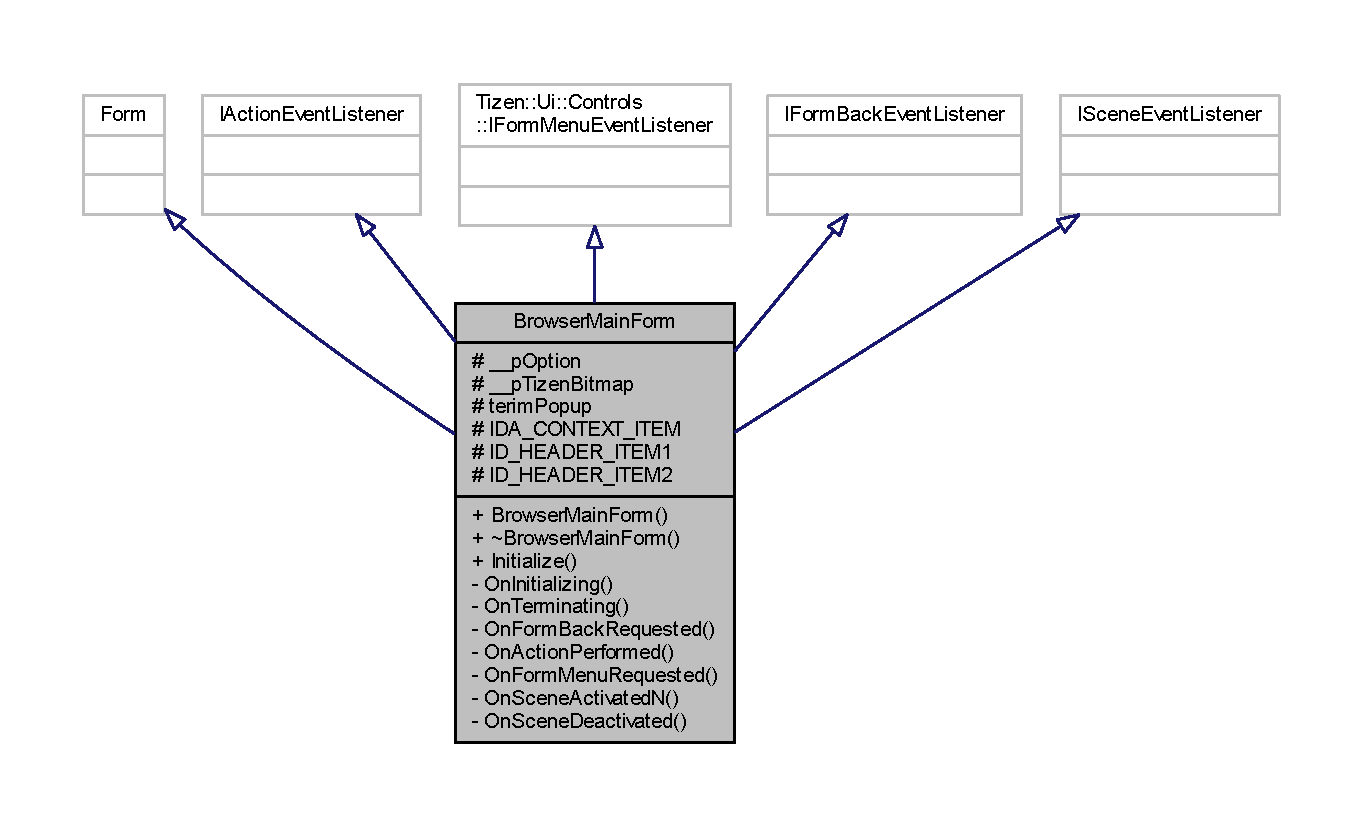
\includegraphics[width=350pt]{class_browser_main_form__inherit__graph}
\end{center}
\end{figure}


Browser\+Main\+Form에 대한 협력 다이어그램\+:
\nopagebreak
\begin{figure}[H]
\begin{center}
\leavevmode
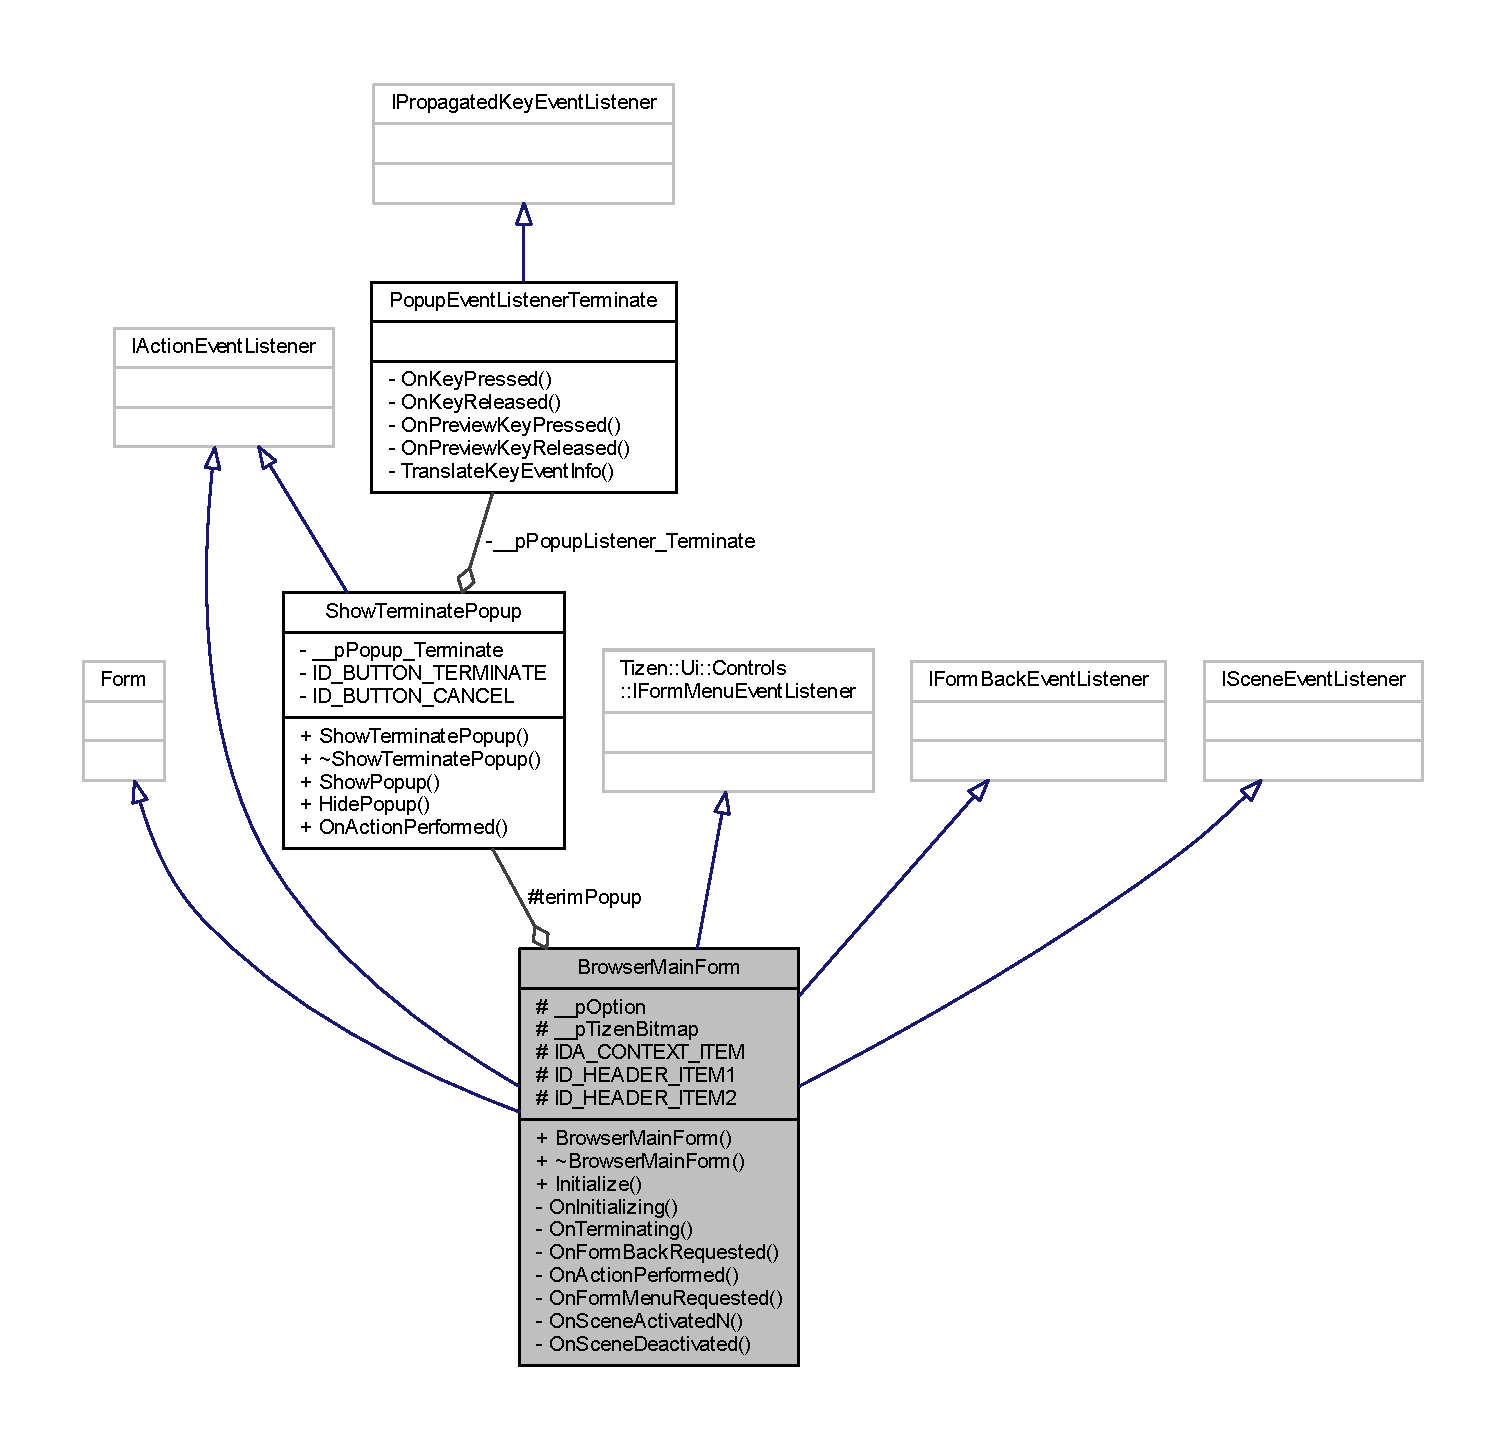
\includegraphics[width=350pt]{class_browser_main_form__coll__graph}
\end{center}
\end{figure}
\subsection*{Public 멤버 함수}
\begin{DoxyCompactItemize}
\item 
\hyperlink{class_browser_main_form_a8d1371e75706b74696b98fd7844fa944}{Browser\+Main\+Form} (void)
\item 
virtual \hyperlink{class_browser_main_form_a5b2bbb6ac4772c7ae7d15b46328afeb6}{$\sim$\+Browser\+Main\+Form} (void)
\item 
bool \hyperlink{class_browser_main_form_a738a1181319a716227fd2ae0feb26c98}{Initialize} (void)
\end{DoxyCompactItemize}
\subsection*{Protected 속성}
\begin{DoxyCompactItemize}
\item 
Tizen\+::\+Ui\+::\+Controls\+::\+Option\+Menu $\ast$ \hyperlink{class_browser_main_form_a6767421f0f61a506e9b187449676fda2}{\+\_\+\+\_\+p\+Option}
\item 
Tizen\+::\+Graphics\+::\+Bitmap $\ast$ \hyperlink{class_browser_main_form_a9ebb215a8612469b49cd95dee767e9cc}{\+\_\+\+\_\+p\+Tizen\+Bitmap}
\item 
\hyperlink{class_show_terminate_popup}{Show\+Terminate\+Popup} \hyperlink{class_browser_main_form_a80aa3a53602f568da86d0f3931b5a06d}{terim\+Popup}
\end{DoxyCompactItemize}
\subsection*{정적 Protected 속성}
\begin{DoxyCompactItemize}
\item 
static const int \hyperlink{class_browser_main_form_a0a7d8a0178a9034082799ab0aeeb28f0}{I\+D\+A\+\_\+\+C\+O\+N\+T\+E\+X\+T\+\_\+\+I\+T\+E\+M} = 103
\item 
static const int \hyperlink{class_browser_main_form_a53791859561cacbbdb6f3089f64fb9fc}{I\+D\+\_\+\+H\+E\+A\+D\+E\+R\+\_\+\+I\+T\+E\+M1} = 101
\item 
static const int \hyperlink{class_browser_main_form_ab0a39b9df377880f65a4753679f43864}{I\+D\+\_\+\+H\+E\+A\+D\+E\+R\+\_\+\+I\+T\+E\+M2} = 102
\end{DoxyCompactItemize}
\subsection*{Private 멤버 함수}
\begin{DoxyCompactItemize}
\item 
virtual result \hyperlink{class_browser_main_form_ae255219c114d47061ee45bd3f46764fd}{On\+Initializing} (void)
\item 
virtual result \hyperlink{class_browser_main_form_a02d722d1c1ba5fd373bf687ef64eaec2}{On\+Terminating} (void)
\item 
virtual void \hyperlink{class_browser_main_form_a63ee65c2094bf2fba5b05d7bc3d79c75}{On\+Form\+Back\+Requested} (Tizen\+::\+Ui\+::\+Controls\+::\+Form \&source)
\item 
virtual void \hyperlink{class_browser_main_form_a6bdcd8ad801f22d26e080329c802e8c5}{On\+Action\+Performed} (const Tizen\+::\+Ui\+::\+Control \&source, int action\+Id)
\item 
virtual void \hyperlink{class_browser_main_form_a5617fd83776b9a4023f7393471d1b29f}{On\+Form\+Menu\+Requested} (Tizen\+::\+Ui\+::\+Controls\+::\+Form \&source)
\item 
void \hyperlink{class_browser_main_form_ab4dda0a9d8e78bc5cfd18c55514836a1}{On\+Scene\+Activated\+N} (const Tizen\+::\+Ui\+::\+Scenes\+::\+Scene\+Id \&previous\+Scene\+Id, const Tizen\+::\+Ui\+::\+Scenes\+::\+Scene\+Id \&current\+Scene\+Id, Tizen\+::\+Base\+::\+Collection\+::\+I\+List $\ast$p\+Args)
\item 
void \hyperlink{class_browser_main_form_ae128a257f33eead52e36476659e0e798}{On\+Scene\+Deactivated} (const Tizen\+::\+Ui\+::\+Scenes\+::\+Scene\+Id \&current\+Scene\+Id, const Tizen\+::\+Ui\+::\+Scenes\+::\+Scene\+Id \&next\+Scene\+Id)
\end{DoxyCompactItemize}


\subsection{상세한 설명}
File Browser Form을 구성해주는 Class. 

Password를 변경할 수 있는 Option Menu와 File Browser Form의 Header를 정의해 주는 Class \begin{DoxyDate}{날짜}
2014-\/12-\/13 
\end{DoxyDate}
\begin{DoxyVersion}{버전}
0.\+0.\+1 
\end{DoxyVersion}


Browser\+Main\+Form.\+h 파일의 19 번째 라인에서 정의되었습니다.



\subsection{생성자 \& 소멸자 문서화}
\hypertarget{class_browser_main_form_a8d1371e75706b74696b98fd7844fa944}{\index{Browser\+Main\+Form@{Browser\+Main\+Form}!Browser\+Main\+Form@{Browser\+Main\+Form}}
\index{Browser\+Main\+Form@{Browser\+Main\+Form}!Browser\+Main\+Form@{Browser\+Main\+Form}}
\subsubsection[{Browser\+Main\+Form}]{\setlength{\rightskip}{0pt plus 5cm}Browser\+Main\+Form\+::\+Browser\+Main\+Form (
\begin{DoxyParamCaption}
\item[{void}]{}
\end{DoxyParamCaption}
)}}\label{class_browser_main_form_a8d1371e75706b74696b98fd7844fa944}


Browser\+Main\+Form.\+cpp 파일의 20 번째 라인에서 정의되었습니다.


\begin{DoxyCode}
20                                      \{
21 \}
\end{DoxyCode}
\hypertarget{class_browser_main_form_a5b2bbb6ac4772c7ae7d15b46328afeb6}{\index{Browser\+Main\+Form@{Browser\+Main\+Form}!````~Browser\+Main\+Form@{$\sim$\+Browser\+Main\+Form}}
\index{````~Browser\+Main\+Form@{$\sim$\+Browser\+Main\+Form}!Browser\+Main\+Form@{Browser\+Main\+Form}}
\subsubsection[{$\sim$\+Browser\+Main\+Form}]{\setlength{\rightskip}{0pt plus 5cm}Browser\+Main\+Form\+::$\sim$\+Browser\+Main\+Form (
\begin{DoxyParamCaption}
\item[{void}]{}
\end{DoxyParamCaption}
)\hspace{0.3cm}{\ttfamily [virtual]}}}\label{class_browser_main_form_a5b2bbb6ac4772c7ae7d15b46328afeb6}


Browser\+Main\+Form.\+cpp 파일의 23 번째 라인에서 정의되었습니다.


\begin{DoxyCode}
23                                       \{
24 \}
\end{DoxyCode}


\subsection{멤버 함수 문서화}
\hypertarget{class_browser_main_form_a738a1181319a716227fd2ae0feb26c98}{\index{Browser\+Main\+Form@{Browser\+Main\+Form}!Initialize@{Initialize}}
\index{Initialize@{Initialize}!Browser\+Main\+Form@{Browser\+Main\+Form}}
\subsubsection[{Initialize}]{\setlength{\rightskip}{0pt plus 5cm}bool Browser\+Main\+Form\+::\+Initialize (
\begin{DoxyParamCaption}
\item[{void}]{}
\end{DoxyParamCaption}
)}}\label{class_browser_main_form_a738a1181319a716227fd2ae0feb26c98}


Browser\+Main\+Form.\+cpp 파일의 26 번째 라인에서 정의되었습니다.


\begin{DoxyCode}
26                                      \{
27     result r = Construct(\hyperlink{_app_resource_id_8h_a6fd4bc3c3d1627e5616fad131142de9c}{IDF\_FILE\_BROWSER\_FORM});
28     TryReturn(r == E\_SUCCESS, \textcolor{keyword}{false}, \textcolor{stringliteral}{"Failed to construct form"});
29 
30     \textcolor{keywordflow}{return} \textcolor{keyword}{true};
31 \}
\end{DoxyCode}


이 함수를 호출하는 함수들에 대한 그래프입니다.\+:
\nopagebreak
\begin{figure}[H]
\begin{center}
\leavevmode
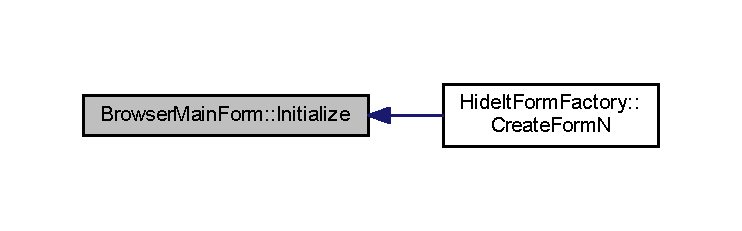
\includegraphics[width=350pt]{class_browser_main_form_a738a1181319a716227fd2ae0feb26c98_icgraph}
\end{center}
\end{figure}


\hypertarget{class_browser_main_form_a6bdcd8ad801f22d26e080329c802e8c5}{\index{Browser\+Main\+Form@{Browser\+Main\+Form}!On\+Action\+Performed@{On\+Action\+Performed}}
\index{On\+Action\+Performed@{On\+Action\+Performed}!Browser\+Main\+Form@{Browser\+Main\+Form}}
\subsubsection[{On\+Action\+Performed}]{\setlength{\rightskip}{0pt plus 5cm}void Browser\+Main\+Form\+::\+On\+Action\+Performed (
\begin{DoxyParamCaption}
\item[{const Tizen\+::\+Ui\+::\+Control \&}]{source, }
\item[{int}]{action\+Id}
\end{DoxyParamCaption}
)\hspace{0.3cm}{\ttfamily [private]}, {\ttfamily [virtual]}}}\label{class_browser_main_form_a6bdcd8ad801f22d26e080329c802e8c5}


Browser\+Main\+Form.\+cpp 파일의 78 번째 라인에서 정의되었습니다.


\begin{DoxyCode}
79                       \{
80     SceneManager* pSceneManager = SceneManager::GetInstance();
81     AppAssert(pSceneManager);
82 
83     \textcolor{keywordflow}{switch} (actionId) \{
84     \textcolor{keywordflow}{case} \hyperlink{class_browser_main_form_a53791859561cacbbdb6f3089f64fb9fc}{ID\_HEADER\_ITEM1}:
85         AppLog(\textcolor{stringliteral}{"ITME1"});
86         pSceneManager->GoForward(
87                 ForwardSceneTransition(\hyperlink{_scene_register_8h_ad2cc89ed96c8bd4c94f954f01ef0f56e}{SCENE\_FILEBROWSER\_MANAGEMENT}));
88         \textcolor{keywordflow}{break};
89     \textcolor{keywordflow}{case} \hyperlink{class_browser_main_form_ab0a39b9df377880f65a4753679f43864}{ID\_HEADER\_ITEM2}:
90         AppLog(\textcolor{stringliteral}{"ITME2"});
91         pSceneManager->GoForward(
92                 ForwardSceneTransition(\hyperlink{_scene_register_8h_a941a02ceb430e35a99e905974dd4faf3}{SCENE\_FILEBROWSER\_HIDDEN}));
93         \textcolor{keywordflow}{break};
94     \textcolor{keywordflow}{case} \hyperlink{class_browser_main_form_a0a7d8a0178a9034082799ab0aeeb28f0}{IDA\_CONTEXT\_ITEM}:
95         pSceneManager->GoForward(
96                 ForwardSceneTransition(\hyperlink{_scene_register_8h_ae2da98cb726565d357021f7d4e0b914e}{SCENE\_SETTING},
97                         SCENE\_TRANSITION\_ANIMATION\_TYPE\_FADE\_IN\_OUT,
98                         SCENE\_HISTORY\_OPTION\_NO\_HISTORY,
99                         SCENE\_DESTROY\_OPTION\_KEEP));
100         \textcolor{keywordflow}{break};
101     \textcolor{keywordflow}{default}:
102         \textcolor{keywordflow}{break};
103     \}
104 \}
\end{DoxyCode}
\hypertarget{class_browser_main_form_a63ee65c2094bf2fba5b05d7bc3d79c75}{\index{Browser\+Main\+Form@{Browser\+Main\+Form}!On\+Form\+Back\+Requested@{On\+Form\+Back\+Requested}}
\index{On\+Form\+Back\+Requested@{On\+Form\+Back\+Requested}!Browser\+Main\+Form@{Browser\+Main\+Form}}
\subsubsection[{On\+Form\+Back\+Requested}]{\setlength{\rightskip}{0pt plus 5cm}void Browser\+Main\+Form\+::\+On\+Form\+Back\+Requested (
\begin{DoxyParamCaption}
\item[{Tizen\+::\+Ui\+::\+Controls\+::\+Form \&}]{source}
\end{DoxyParamCaption}
)\hspace{0.3cm}{\ttfamily [private]}, {\ttfamily [virtual]}}}\label{class_browser_main_form_a63ee65c2094bf2fba5b05d7bc3d79c75}


Browser\+Main\+Form.\+cpp 파일의 106 번째 라인에서 정의되었습니다.


\begin{DoxyCode}
106                                                                      \{
107     AppLog(\textcolor{stringliteral}{"BackBack Form"});
108 \textcolor{comment}{//  UiApp* pApp = UiApp::GetInstance();}
109 \textcolor{comment}{//  AppAssert(pApp);}
110 \textcolor{comment}{//  pApp->Terminate();}
111     \hyperlink{class_browser_main_form_a80aa3a53602f568da86d0f3931b5a06d}{terimPopup}.\hyperlink{class_show_terminate_popup_aa3424f6b23949489b0e3f674ec9c7c1c}{ShowPopup}();
112 \}
\end{DoxyCode}
\hypertarget{class_browser_main_form_a5617fd83776b9a4023f7393471d1b29f}{\index{Browser\+Main\+Form@{Browser\+Main\+Form}!On\+Form\+Menu\+Requested@{On\+Form\+Menu\+Requested}}
\index{On\+Form\+Menu\+Requested@{On\+Form\+Menu\+Requested}!Browser\+Main\+Form@{Browser\+Main\+Form}}
\subsubsection[{On\+Form\+Menu\+Requested}]{\setlength{\rightskip}{0pt plus 5cm}void Browser\+Main\+Form\+::\+On\+Form\+Menu\+Requested (
\begin{DoxyParamCaption}
\item[{Tizen\+::\+Ui\+::\+Controls\+::\+Form \&}]{source}
\end{DoxyParamCaption}
)\hspace{0.3cm}{\ttfamily [private]}, {\ttfamily [virtual]}}}\label{class_browser_main_form_a5617fd83776b9a4023f7393471d1b29f}


Browser\+Main\+Form.\+cpp 파일의 114 번째 라인에서 정의되었습니다.


\begin{DoxyCode}
114                                                                      \{
115     \hyperlink{class_browser_main_form_a6767421f0f61a506e9b187449676fda2}{\_\_pOption}->SetShowState(\textcolor{keyword}{true});
116     \hyperlink{class_browser_main_form_a6767421f0f61a506e9b187449676fda2}{\_\_pOption}->Show();
117 \}
\end{DoxyCode}
\hypertarget{class_browser_main_form_ae255219c114d47061ee45bd3f46764fd}{\index{Browser\+Main\+Form@{Browser\+Main\+Form}!On\+Initializing@{On\+Initializing}}
\index{On\+Initializing@{On\+Initializing}!Browser\+Main\+Form@{Browser\+Main\+Form}}
\subsubsection[{On\+Initializing}]{\setlength{\rightskip}{0pt plus 5cm}result Browser\+Main\+Form\+::\+On\+Initializing (
\begin{DoxyParamCaption}
\item[{void}]{}
\end{DoxyParamCaption}
)\hspace{0.3cm}{\ttfamily [private]}, {\ttfamily [virtual]}}}\label{class_browser_main_form_ae255219c114d47061ee45bd3f46764fd}


Browser\+Main\+Form.\+cpp 파일의 33 번째 라인에서 정의되었습니다.


\begin{DoxyCode}
33                                            \{
34     result r = E\_SUCCESS;
35 
36     \textcolor{comment}{// TODO: Add your initialization code here}
37     Header* pHeader = GetHeader();
38     \textcolor{keywordflow}{if} (pHeader) \{
39         pHeader->AddActionEventListener(*\textcolor{keyword}{this});
40     \}
41 
42     \textcolor{comment}{// Setup back event listener}
43     \textcolor{comment}{//SetFormBackEventListener(reinterpret\_cast<BrowserTab1*>(GetControl(IDL\_MANAGEMENT\_PANEL)));}
44     \textcolor{comment}{//SetFormBackEventListener(reinterpret\_cast<BrowserTab2*>(GetControl(IDL\_HIDDEN\_FILES\_PANEL)));}
45 
46     SetFormBackEventListener(\textcolor{keyword}{this});
47 
48     Image pimage;
49     r = pimage.Construct();
50     String filepath = App::GetInstance()->GetAppDataPath();
51     \hyperlink{class_browser_main_form_a9ebb215a8612469b49cd95dee767e9cc}{\_\_pTizenBitmap} = pimage.DecodeN(filepath + L\textcolor{stringliteral}{"icon\_filebrowser.png"},
52             BITMAP\_PIXEL\_FORMAT\_ARGB8888);
53 
54     \textcolor{comment}{// Set-up header}
55     AppAssert(pHeader);
56     pHeader->SetTitleIcon(\hyperlink{class_browser_main_form_a9ebb215a8612469b49cd95dee767e9cc}{\_\_pTizenBitmap});
57 
58     \textcolor{comment}{//Menu part}
59     
60     SetFormMenuEventListener(\textcolor{keyword}{this});
61     \hyperlink{class_browser_main_form_a6767421f0f61a506e9b187449676fda2}{\_\_pOption} = \textcolor{keyword}{new} (std::nothrow) OptionMenu();
62     \hyperlink{class_browser_main_form_a6767421f0f61a506e9b187449676fda2}{\_\_pOption}->Construct();
63     \hyperlink{class_browser_main_form_a6767421f0f61a506e9b187449676fda2}{\_\_pOption}->AddItem(L\textcolor{stringliteral}{"Set Key Expresstion"}, \hyperlink{class_browser_main_form_a0a7d8a0178a9034082799ab0aeeb28f0}{IDA\_CONTEXT\_ITEM});
64     \hyperlink{class_browser_main_form_a6767421f0f61a506e9b187449676fda2}{\_\_pOption}->AddActionEventListener(*\textcolor{keyword}{this});
65     \hyperlink{class_browser_main_form_a6767421f0f61a506e9b187449676fda2}{\_\_pOption}->SetShowState(\textcolor{keyword}{false});
66     \textcolor{comment}{//*/}
67 
68     \textcolor{keywordflow}{return} r;
69 \}
\end{DoxyCode}
\hypertarget{class_browser_main_form_ab4dda0a9d8e78bc5cfd18c55514836a1}{\index{Browser\+Main\+Form@{Browser\+Main\+Form}!On\+Scene\+Activated\+N@{On\+Scene\+Activated\+N}}
\index{On\+Scene\+Activated\+N@{On\+Scene\+Activated\+N}!Browser\+Main\+Form@{Browser\+Main\+Form}}
\subsubsection[{On\+Scene\+Activated\+N}]{\setlength{\rightskip}{0pt plus 5cm}void Browser\+Main\+Form\+::\+On\+Scene\+Activated\+N (
\begin{DoxyParamCaption}
\item[{const Tizen\+::\+Ui\+::\+Scenes\+::\+Scene\+Id \&}]{previous\+Scene\+Id, }
\item[{const Tizen\+::\+Ui\+::\+Scenes\+::\+Scene\+Id \&}]{current\+Scene\+Id, }
\item[{Tizen\+::\+Base\+::\+Collection\+::\+I\+List $\ast$}]{p\+Args}
\end{DoxyParamCaption}
)\hspace{0.3cm}{\ttfamily [private]}}}\label{class_browser_main_form_ab4dda0a9d8e78bc5cfd18c55514836a1}


Browser\+Main\+Form.\+cpp 파일의 119 번째 라인에서 정의되었습니다.


\begin{DoxyCode}
122                                          \{
123 
124 \}
\end{DoxyCode}
\hypertarget{class_browser_main_form_ae128a257f33eead52e36476659e0e798}{\index{Browser\+Main\+Form@{Browser\+Main\+Form}!On\+Scene\+Deactivated@{On\+Scene\+Deactivated}}
\index{On\+Scene\+Deactivated@{On\+Scene\+Deactivated}!Browser\+Main\+Form@{Browser\+Main\+Form}}
\subsubsection[{On\+Scene\+Deactivated}]{\setlength{\rightskip}{0pt plus 5cm}void Browser\+Main\+Form\+::\+On\+Scene\+Deactivated (
\begin{DoxyParamCaption}
\item[{const Tizen\+::\+Ui\+::\+Scenes\+::\+Scene\+Id \&}]{current\+Scene\+Id, }
\item[{const Tizen\+::\+Ui\+::\+Scenes\+::\+Scene\+Id \&}]{next\+Scene\+Id}
\end{DoxyParamCaption}
)\hspace{0.3cm}{\ttfamily [private]}}}\label{class_browser_main_form_ae128a257f33eead52e36476659e0e798}


Browser\+Main\+Form.\+cpp 파일의 126 번째 라인에서 정의되었습니다.


\begin{DoxyCode}
128                                                  \{
129 \}
\end{DoxyCode}
\hypertarget{class_browser_main_form_a02d722d1c1ba5fd373bf687ef64eaec2}{\index{Browser\+Main\+Form@{Browser\+Main\+Form}!On\+Terminating@{On\+Terminating}}
\index{On\+Terminating@{On\+Terminating}!Browser\+Main\+Form@{Browser\+Main\+Form}}
\subsubsection[{On\+Terminating}]{\setlength{\rightskip}{0pt plus 5cm}result Browser\+Main\+Form\+::\+On\+Terminating (
\begin{DoxyParamCaption}
\item[{void}]{}
\end{DoxyParamCaption}
)\hspace{0.3cm}{\ttfamily [private]}, {\ttfamily [virtual]}}}\label{class_browser_main_form_a02d722d1c1ba5fd373bf687ef64eaec2}


Browser\+Main\+Form.\+cpp 파일의 71 번째 라인에서 정의되었습니다.


\begin{DoxyCode}
71                                           \{
72     result r = E\_SUCCESS;
73 
74     \textcolor{comment}{// TODO: Add your termination code here}
75     \textcolor{keywordflow}{return} r;
76 \}
\end{DoxyCode}


\subsection{멤버 데이타 문서화}
\hypertarget{class_browser_main_form_a6767421f0f61a506e9b187449676fda2}{\index{Browser\+Main\+Form@{Browser\+Main\+Form}!\+\_\+\+\_\+p\+Option@{\+\_\+\+\_\+p\+Option}}
\index{\+\_\+\+\_\+p\+Option@{\+\_\+\+\_\+p\+Option}!Browser\+Main\+Form@{Browser\+Main\+Form}}
\subsubsection[{\+\_\+\+\_\+p\+Option}]{\setlength{\rightskip}{0pt plus 5cm}Tizen\+::\+Ui\+::\+Controls\+::\+Option\+Menu$\ast$ Browser\+Main\+Form\+::\+\_\+\+\_\+p\+Option\hspace{0.3cm}{\ttfamily [protected]}}}\label{class_browser_main_form_a6767421f0f61a506e9b187449676fda2}


Browser\+Main\+Form.\+h 파일의 44 번째 라인에서 정의되었습니다.

\hypertarget{class_browser_main_form_a9ebb215a8612469b49cd95dee767e9cc}{\index{Browser\+Main\+Form@{Browser\+Main\+Form}!\+\_\+\+\_\+p\+Tizen\+Bitmap@{\+\_\+\+\_\+p\+Tizen\+Bitmap}}
\index{\+\_\+\+\_\+p\+Tizen\+Bitmap@{\+\_\+\+\_\+p\+Tizen\+Bitmap}!Browser\+Main\+Form@{Browser\+Main\+Form}}
\subsubsection[{\+\_\+\+\_\+p\+Tizen\+Bitmap}]{\setlength{\rightskip}{0pt plus 5cm}Tizen\+::\+Graphics\+::\+Bitmap$\ast$ Browser\+Main\+Form\+::\+\_\+\+\_\+p\+Tizen\+Bitmap\hspace{0.3cm}{\ttfamily [protected]}}}\label{class_browser_main_form_a9ebb215a8612469b49cd95dee767e9cc}


Browser\+Main\+Form.\+h 파일의 48 번째 라인에서 정의되었습니다.

\hypertarget{class_browser_main_form_a53791859561cacbbdb6f3089f64fb9fc}{\index{Browser\+Main\+Form@{Browser\+Main\+Form}!I\+D\+\_\+\+H\+E\+A\+D\+E\+R\+\_\+\+I\+T\+E\+M1@{I\+D\+\_\+\+H\+E\+A\+D\+E\+R\+\_\+\+I\+T\+E\+M1}}
\index{I\+D\+\_\+\+H\+E\+A\+D\+E\+R\+\_\+\+I\+T\+E\+M1@{I\+D\+\_\+\+H\+E\+A\+D\+E\+R\+\_\+\+I\+T\+E\+M1}!Browser\+Main\+Form@{Browser\+Main\+Form}}
\subsubsection[{I\+D\+\_\+\+H\+E\+A\+D\+E\+R\+\_\+\+I\+T\+E\+M1}]{\setlength{\rightskip}{0pt plus 5cm}const int Browser\+Main\+Form\+::\+I\+D\+\_\+\+H\+E\+A\+D\+E\+R\+\_\+\+I\+T\+E\+M1 = 101\hspace{0.3cm}{\ttfamily [static]}, {\ttfamily [protected]}}}\label{class_browser_main_form_a53791859561cacbbdb6f3089f64fb9fc}


Browser\+Main\+Form.\+h 파일의 46 번째 라인에서 정의되었습니다.

\hypertarget{class_browser_main_form_ab0a39b9df377880f65a4753679f43864}{\index{Browser\+Main\+Form@{Browser\+Main\+Form}!I\+D\+\_\+\+H\+E\+A\+D\+E\+R\+\_\+\+I\+T\+E\+M2@{I\+D\+\_\+\+H\+E\+A\+D\+E\+R\+\_\+\+I\+T\+E\+M2}}
\index{I\+D\+\_\+\+H\+E\+A\+D\+E\+R\+\_\+\+I\+T\+E\+M2@{I\+D\+\_\+\+H\+E\+A\+D\+E\+R\+\_\+\+I\+T\+E\+M2}!Browser\+Main\+Form@{Browser\+Main\+Form}}
\subsubsection[{I\+D\+\_\+\+H\+E\+A\+D\+E\+R\+\_\+\+I\+T\+E\+M2}]{\setlength{\rightskip}{0pt plus 5cm}const int Browser\+Main\+Form\+::\+I\+D\+\_\+\+H\+E\+A\+D\+E\+R\+\_\+\+I\+T\+E\+M2 = 102\hspace{0.3cm}{\ttfamily [static]}, {\ttfamily [protected]}}}\label{class_browser_main_form_ab0a39b9df377880f65a4753679f43864}


Browser\+Main\+Form.\+h 파일의 47 번째 라인에서 정의되었습니다.

\hypertarget{class_browser_main_form_a0a7d8a0178a9034082799ab0aeeb28f0}{\index{Browser\+Main\+Form@{Browser\+Main\+Form}!I\+D\+A\+\_\+\+C\+O\+N\+T\+E\+X\+T\+\_\+\+I\+T\+E\+M@{I\+D\+A\+\_\+\+C\+O\+N\+T\+E\+X\+T\+\_\+\+I\+T\+E\+M}}
\index{I\+D\+A\+\_\+\+C\+O\+N\+T\+E\+X\+T\+\_\+\+I\+T\+E\+M@{I\+D\+A\+\_\+\+C\+O\+N\+T\+E\+X\+T\+\_\+\+I\+T\+E\+M}!Browser\+Main\+Form@{Browser\+Main\+Form}}
\subsubsection[{I\+D\+A\+\_\+\+C\+O\+N\+T\+E\+X\+T\+\_\+\+I\+T\+E\+M}]{\setlength{\rightskip}{0pt plus 5cm}const int Browser\+Main\+Form\+::\+I\+D\+A\+\_\+\+C\+O\+N\+T\+E\+X\+T\+\_\+\+I\+T\+E\+M = 103\hspace{0.3cm}{\ttfamily [static]}, {\ttfamily [protected]}}}\label{class_browser_main_form_a0a7d8a0178a9034082799ab0aeeb28f0}


Browser\+Main\+Form.\+h 파일의 45 번째 라인에서 정의되었습니다.

\hypertarget{class_browser_main_form_a80aa3a53602f568da86d0f3931b5a06d}{\index{Browser\+Main\+Form@{Browser\+Main\+Form}!terim\+Popup@{terim\+Popup}}
\index{terim\+Popup@{terim\+Popup}!Browser\+Main\+Form@{Browser\+Main\+Form}}
\subsubsection[{terim\+Popup}]{\setlength{\rightskip}{0pt plus 5cm}{\bf Show\+Terminate\+Popup} Browser\+Main\+Form\+::terim\+Popup\hspace{0.3cm}{\ttfamily [protected]}}}\label{class_browser_main_form_a80aa3a53602f568da86d0f3931b5a06d}


Browser\+Main\+Form.\+h 파일의 49 번째 라인에서 정의되었습니다.



이 클래스에 대한 문서화 페이지는 다음의 파일들로부터 생성되었습니다.\+:\begin{DoxyCompactItemize}
\item 
inc/\hyperlink{_browser_main_form_8h}{Browser\+Main\+Form.\+h}\item 
src/\+File\+Browser/\hyperlink{_browser_main_form_8cpp}{Browser\+Main\+Form.\+cpp}\end{DoxyCompactItemize}

\hypertarget{class_browser_tab1}{\section{Browser\+Tab1 클래스 참조}
\label{class_browser_tab1}\index{Browser\+Tab1@{Browser\+Tab1}}
}


File Browser의 Management tab을 구성해주는 Class.  




{\ttfamily \#include $<$Browser\+Tab1.\+h$>$}



Browser\+Tab1에 대한 상속 다이어그램 \+: 
\nopagebreak
\begin{figure}[H]
\begin{center}
\leavevmode
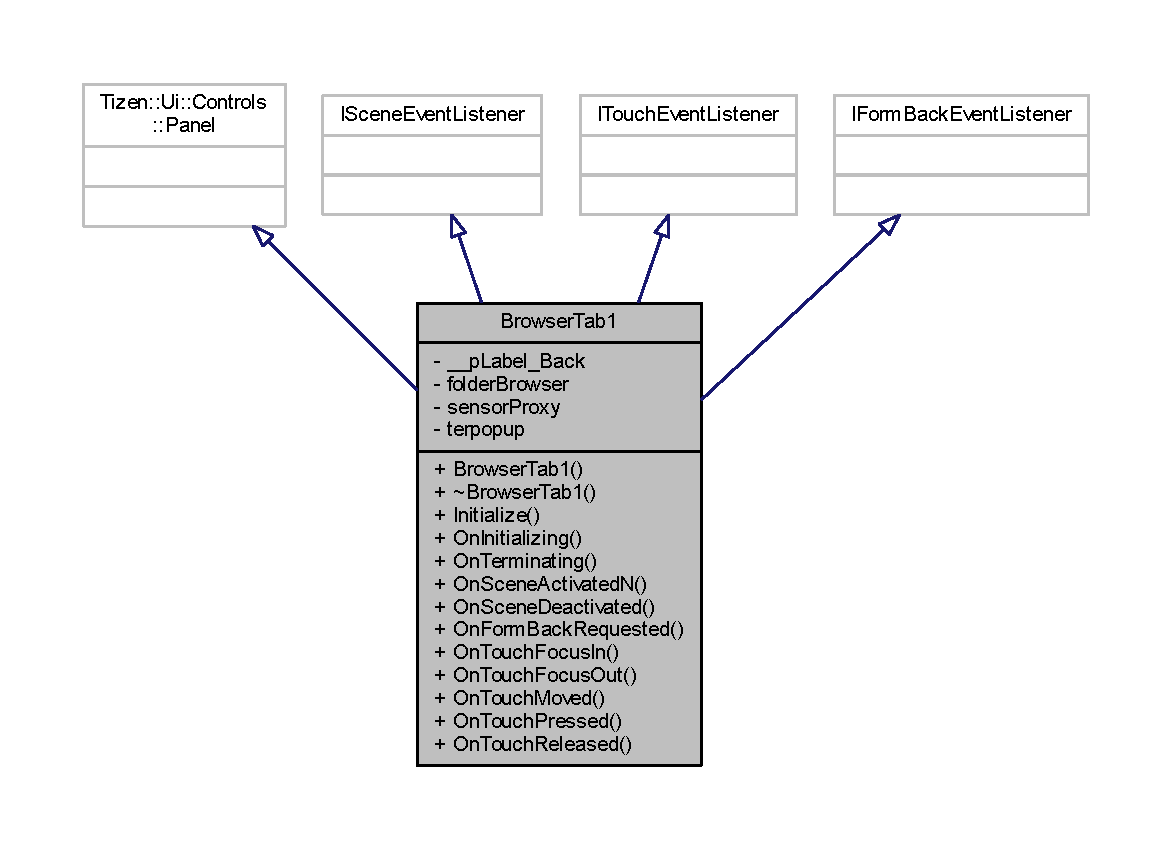
\includegraphics[width=350pt]{class_browser_tab1__inherit__graph}
\end{center}
\end{figure}


Browser\+Tab1에 대한 협력 다이어그램\+:
\nopagebreak
\begin{figure}[H]
\begin{center}
\leavevmode
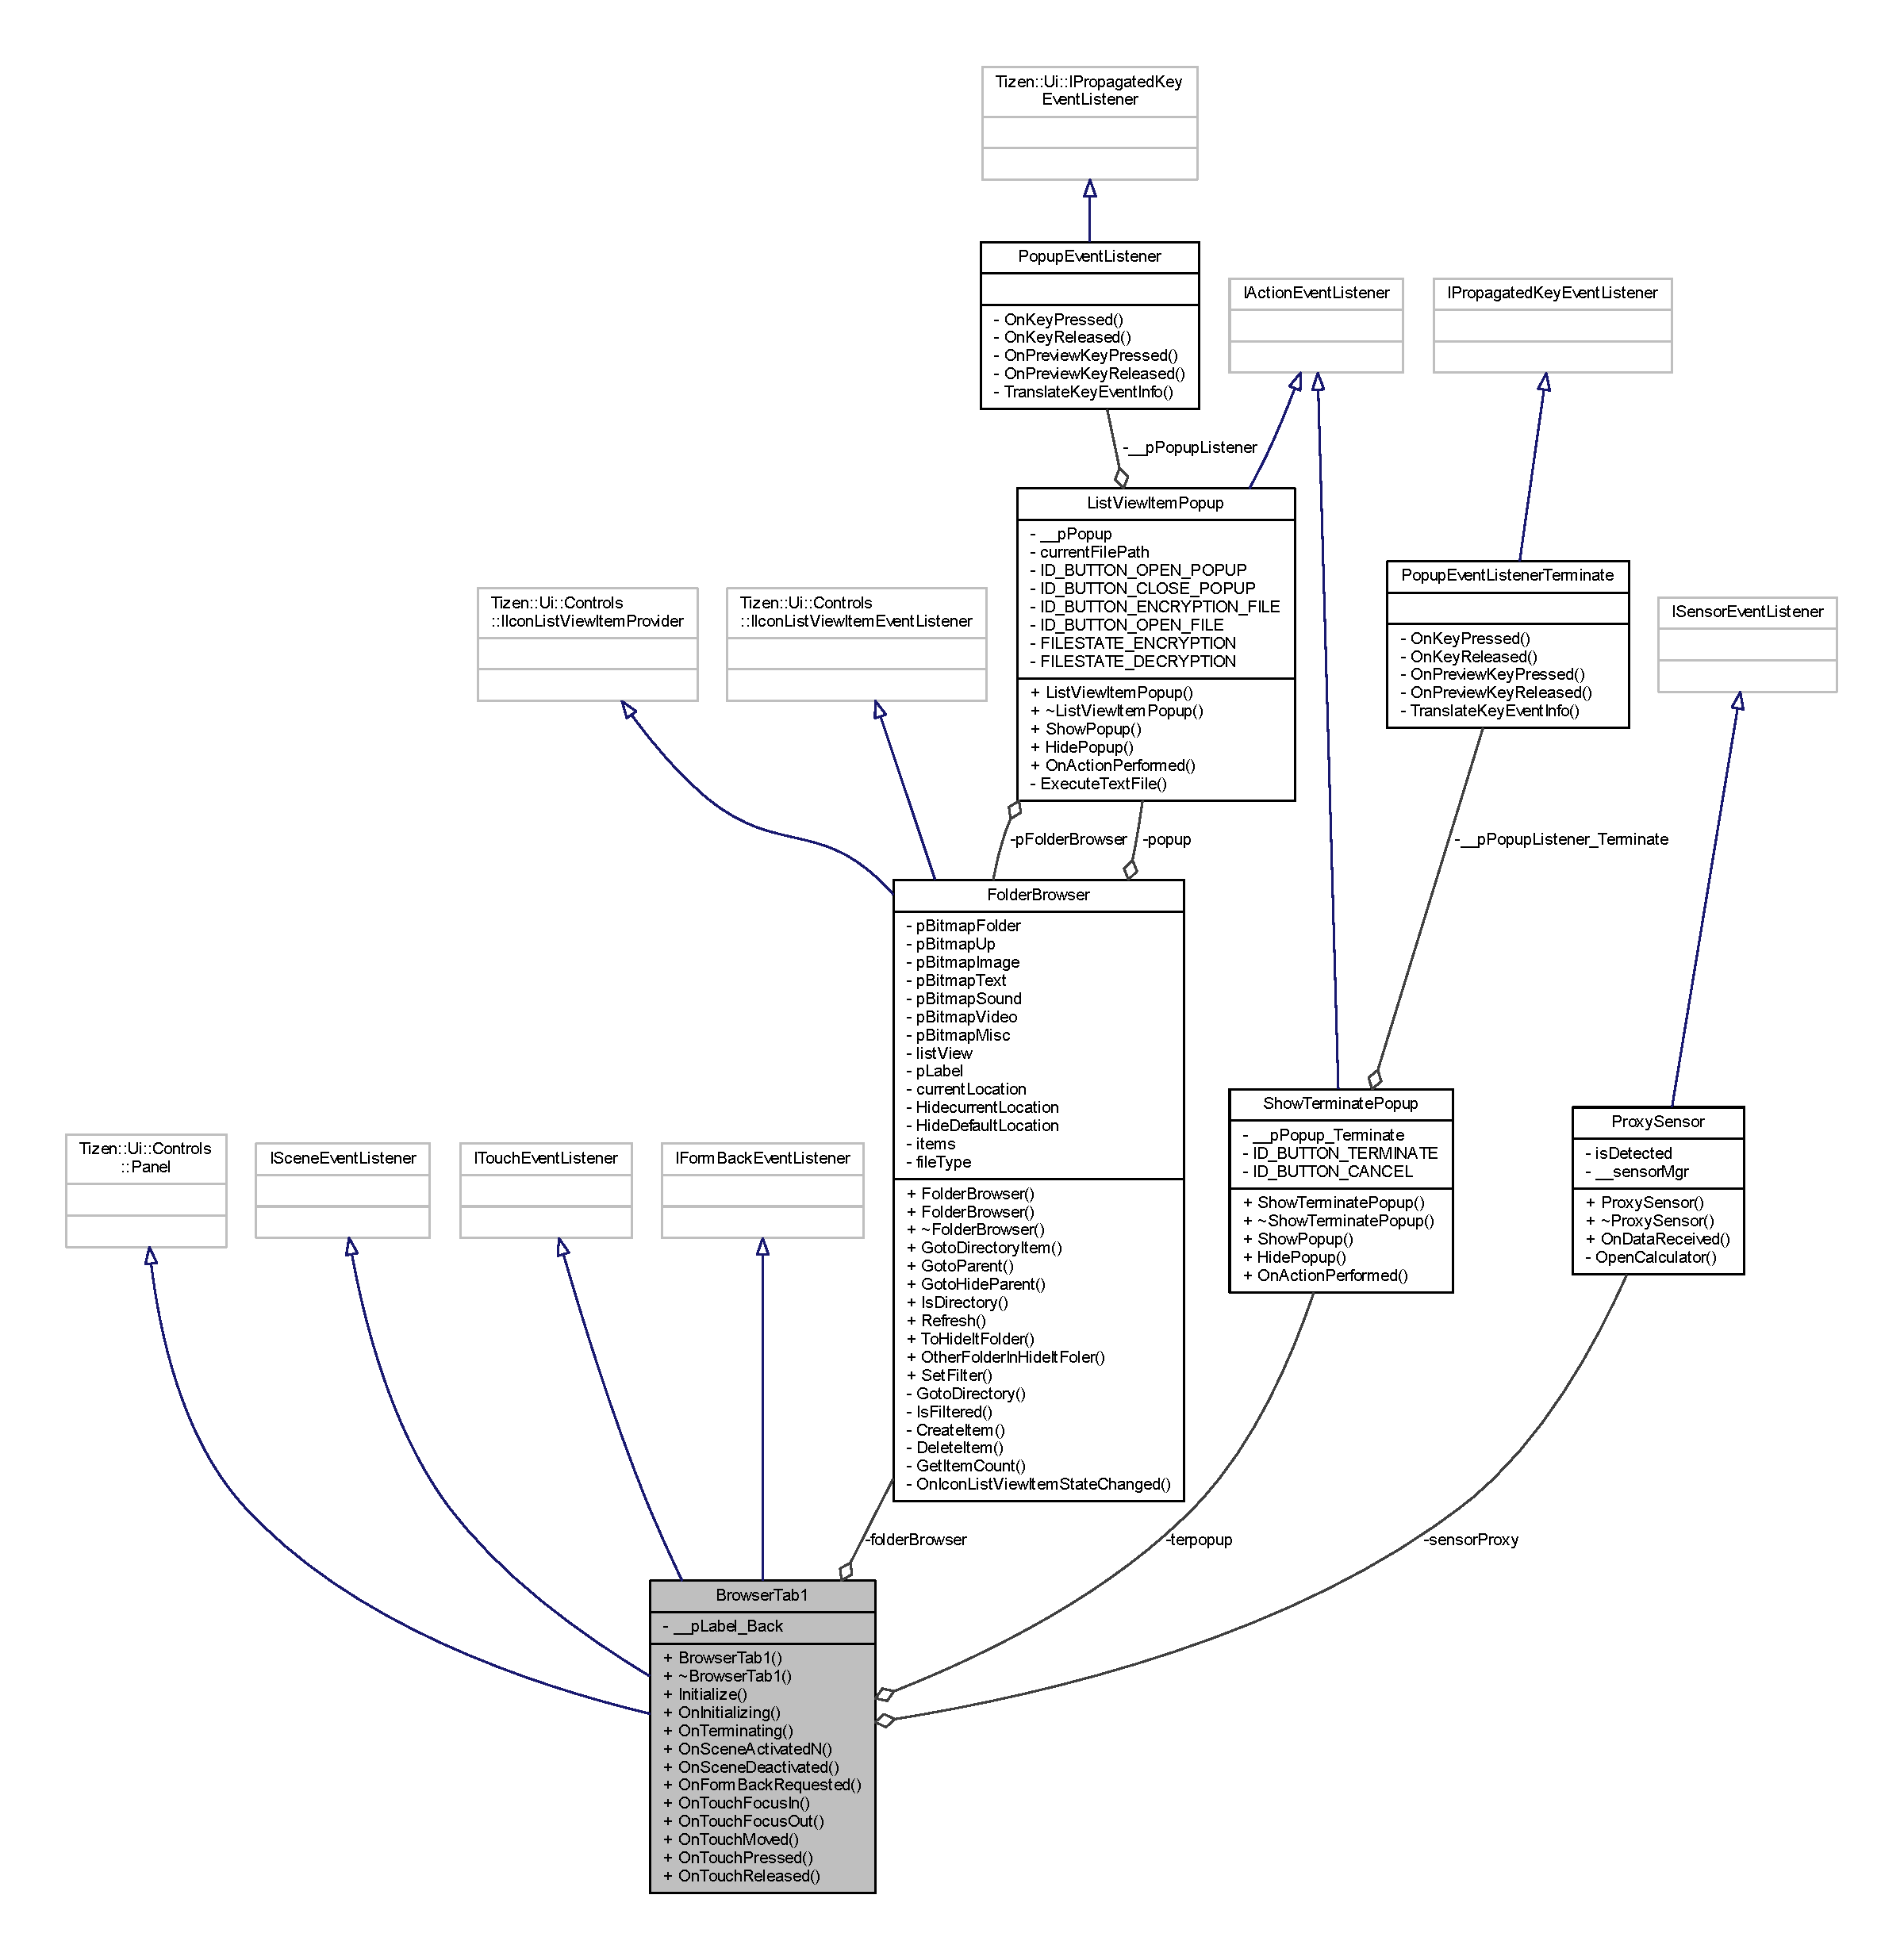
\includegraphics[width=350pt]{class_browser_tab1__coll__graph}
\end{center}
\end{figure}
\subsection*{Public 멤버 함수}
\begin{DoxyCompactItemize}
\item 
\hyperlink{class_browser_tab1_a42e0e4ea28b2debcfb5ee0e5dc2ecf09}{Browser\+Tab1} (void)
\item 
virtual \hyperlink{class_browser_tab1_ad1024dd5d5945a5d29be9306d5ae3013}{$\sim$\+Browser\+Tab1} (void)
\item 
bool \hyperlink{class_browser_tab1_ae8f2b22d3dd917b599c7f46549079687}{Initialize} (void)
\item 
virtual result \hyperlink{class_browser_tab1_ab3fa028108d66af5fa6bbe088cf44e5f}{On\+Initializing} (void)
\item 
virtual result \hyperlink{class_browser_tab1_aa87b7496a627892df34a96138337d7ca}{On\+Terminating} (void)
\item 
virtual void \hyperlink{class_browser_tab1_a6a40e7124eb0c67a3986b4122befe3d5}{On\+Scene\+Activated\+N} (const Tizen\+::\+Ui\+::\+Scenes\+::\+Scene\+Id \&previous\+Scene\+Id, const Tizen\+::\+Ui\+::\+Scenes\+::\+Scene\+Id \&current\+Scene\+Id, Tizen\+::\+Base\+::\+Collection\+::\+I\+List $\ast$p\+Args)
\item 
virtual void \hyperlink{class_browser_tab1_a572592e61e494f61b62b71e60270ef1d}{On\+Scene\+Deactivated} (const Tizen\+::\+Ui\+::\+Scenes\+::\+Scene\+Id \&current\+Scene\+Id, const Tizen\+::\+Ui\+::\+Scenes\+::\+Scene\+Id \&next\+Scene\+Id)
\item 
virtual void \hyperlink{class_browser_tab1_a535e5fc3e6a2e82ad029be81652d5509}{On\+Form\+Back\+Requested} (Tizen\+::\+Ui\+::\+Controls\+::\+Form \&source)
\item 
virtual void \hyperlink{class_browser_tab1_a5da5021cbb84ac88708ed984e1eca853}{On\+Touch\+Focus\+In} (const Tizen\+::\+Ui\+::\+Control \&source, const Tizen\+::\+Graphics\+::\+Point \&current\+Position, const Tizen\+::\+Ui\+::\+Touch\+Event\+Info \&touch\+Info)
\item 
virtual void \hyperlink{class_browser_tab1_ae25d906cbfcd2505a3669111d672e79b}{On\+Touch\+Focus\+Out} (const Tizen\+::\+Ui\+::\+Control \&source, const Tizen\+::\+Graphics\+::\+Point \&current\+Position, const Tizen\+::\+Ui\+::\+Touch\+Event\+Info \&touch\+Info)
\item 
virtual void \hyperlink{class_browser_tab1_a7d70ed9cfa3f2ed1df6d0aeacb21ee48}{On\+Touch\+Moved} (const Tizen\+::\+Ui\+::\+Control \&source, const Tizen\+::\+Graphics\+::\+Point \&current\+Position, const Tizen\+::\+Ui\+::\+Touch\+Event\+Info \&touch\+Info)
\item 
virtual void \hyperlink{class_browser_tab1_af18debc3d96a67c757408b69efff9d2f}{On\+Touch\+Pressed} (const Tizen\+::\+Ui\+::\+Control \&source, const Tizen\+::\+Graphics\+::\+Point \&current\+Position, const Tizen\+::\+Ui\+::\+Touch\+Event\+Info \&touch\+Info)
\item 
virtual void \hyperlink{class_browser_tab1_a958c88e3bc8de62132379fd12b9b1f97}{On\+Touch\+Released} (const Tizen\+::\+Ui\+::\+Control \&source, const Tizen\+::\+Graphics\+::\+Point \&current\+Position, const Tizen\+::\+Ui\+::\+Touch\+Event\+Info \&touch\+Info)
\end{DoxyCompactItemize}
\subsection*{Private 속성}
\begin{DoxyCompactItemize}
\item 
Tizen\+::\+Ui\+::\+Controls\+::\+Label $\ast$ \hyperlink{class_browser_tab1_ad072e2bcaa2a03d684ddfddd0d8dea77}{\+\_\+\+\_\+p\+Label\+\_\+\+Back}
\item 
\hyperlink{class_folder_browser}{Folder\+Browser} $\ast$ \hyperlink{class_browser_tab1_a2a514b5068c1222055a103c67abeeb2a}{folder\+Browser}
\item 
\hyperlink{class_proxy_sensor}{Proxy\+Sensor} $\ast$ \hyperlink{class_browser_tab1_a7dc2f8e362bbc5c88cedb59e0b38cbea}{sensor\+Proxy}
\item 
\hyperlink{class_show_terminate_popup}{Show\+Terminate\+Popup} \hyperlink{class_browser_tab1_a69eaa59d7c5277fe9819b3b7fa7bbea4}{terpopup}
\end{DoxyCompactItemize}


\subsection{상세한 설명}
File Browser의 Management tab을 구성해주는 Class. 

\begin{DoxyDate}{날짜}
2014-\/12-\/13 
\end{DoxyDate}
\begin{DoxyVersion}{버전}
0.\+0.\+1 
\end{DoxyVersion}


Browser\+Tab1.\+h 파일의 22 번째 라인에서 정의되었습니다.



\subsection{생성자 \& 소멸자 문서화}
\hypertarget{class_browser_tab1_a42e0e4ea28b2debcfb5ee0e5dc2ecf09}{\index{Browser\+Tab1@{Browser\+Tab1}!Browser\+Tab1@{Browser\+Tab1}}
\index{Browser\+Tab1@{Browser\+Tab1}!Browser\+Tab1@{Browser\+Tab1}}
\subsubsection[{Browser\+Tab1}]{\setlength{\rightskip}{0pt plus 5cm}Browser\+Tab1\+::\+Browser\+Tab1 (
\begin{DoxyParamCaption}
\item[{void}]{}
\end{DoxyParamCaption}
)}}\label{class_browser_tab1_a42e0e4ea28b2debcfb5ee0e5dc2ecf09}


Browser\+Tab1.\+cpp 파일의 11 번째 라인에서 정의되었습니다.


\begin{DoxyCode}
11                              \{
12     AppLog(\textcolor{stringliteral}{"Tap1 Creating"});
13 \}
\end{DoxyCode}
\hypertarget{class_browser_tab1_ad1024dd5d5945a5d29be9306d5ae3013}{\index{Browser\+Tab1@{Browser\+Tab1}!````~Browser\+Tab1@{$\sim$\+Browser\+Tab1}}
\index{````~Browser\+Tab1@{$\sim$\+Browser\+Tab1}!Browser\+Tab1@{Browser\+Tab1}}
\subsubsection[{$\sim$\+Browser\+Tab1}]{\setlength{\rightskip}{0pt plus 5cm}Browser\+Tab1\+::$\sim$\+Browser\+Tab1 (
\begin{DoxyParamCaption}
\item[{void}]{}
\end{DoxyParamCaption}
)\hspace{0.3cm}{\ttfamily [virtual]}}}\label{class_browser_tab1_ad1024dd5d5945a5d29be9306d5ae3013}


Browser\+Tab1.\+cpp 파일의 15 번째 라인에서 정의되었습니다.


\begin{DoxyCode}
15                               \{
16 
17 \}
\end{DoxyCode}


\subsection{멤버 함수 문서화}
\hypertarget{class_browser_tab1_ae8f2b22d3dd917b599c7f46549079687}{\index{Browser\+Tab1@{Browser\+Tab1}!Initialize@{Initialize}}
\index{Initialize@{Initialize}!Browser\+Tab1@{Browser\+Tab1}}
\subsubsection[{Initialize}]{\setlength{\rightskip}{0pt plus 5cm}bool Browser\+Tab1\+::\+Initialize (
\begin{DoxyParamCaption}
\item[{void}]{}
\end{DoxyParamCaption}
)}}\label{class_browser_tab1_ae8f2b22d3dd917b599c7f46549079687}


Browser\+Tab1.\+cpp 파일의 19 번째 라인에서 정의되었습니다.


\begin{DoxyCode}
19                                  \{
20     result r = Construct(\hyperlink{_app_resource_id_8h_aa4977f921a656ca704b1c6cf4cba205a}{IDL\_MANAGEMENT\_PANEL});
21     \textcolor{keywordflow}{if} (IsFailed(r)) \{
22         \textcolor{keywordflow}{return} \textcolor{keyword}{false};
23     \}
24     \textcolor{keywordflow}{return} \textcolor{keyword}{true};
25 \}
\end{DoxyCode}


이 함수를 호출하는 함수들에 대한 그래프입니다.\+:
\nopagebreak
\begin{figure}[H]
\begin{center}
\leavevmode
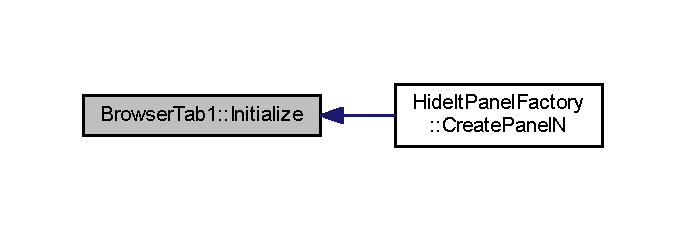
\includegraphics[width=329pt]{class_browser_tab1_ae8f2b22d3dd917b599c7f46549079687_icgraph}
\end{center}
\end{figure}


\hypertarget{class_browser_tab1_a535e5fc3e6a2e82ad029be81652d5509}{\index{Browser\+Tab1@{Browser\+Tab1}!On\+Form\+Back\+Requested@{On\+Form\+Back\+Requested}}
\index{On\+Form\+Back\+Requested@{On\+Form\+Back\+Requested}!Browser\+Tab1@{Browser\+Tab1}}
\subsubsection[{On\+Form\+Back\+Requested}]{\setlength{\rightskip}{0pt plus 5cm}void Browser\+Tab1\+::\+On\+Form\+Back\+Requested (
\begin{DoxyParamCaption}
\item[{Tizen\+::\+Ui\+::\+Controls\+::\+Form \&}]{source}
\end{DoxyParamCaption}
)\hspace{0.3cm}{\ttfamily [virtual]}}}\label{class_browser_tab1_a535e5fc3e6a2e82ad029be81652d5509}


Browser\+Tab1.\+cpp 파일의 100 번째 라인에서 정의되었습니다.


\begin{DoxyCode}
100                                                                  \{
101     \textcolor{comment}{/*}
102 \textcolor{comment}{    AppLog("BackBack");}
103 \textcolor{comment}{    UiApp* pApp = UiApp::GetInstance();}
104 \textcolor{comment}{    AppAssert(pApp);}
105 \textcolor{comment}{    pApp->Terminate();}
106 \textcolor{comment}{     */}
107     AppLog(\textcolor{stringliteral}{"BackBack Tab1 "});
108     \hyperlink{class_browser_tab1_a69eaa59d7c5277fe9819b3b7fa7bbea4}{terpopup}.\hyperlink{class_show_terminate_popup_aa3424f6b23949489b0e3f674ec9c7c1c}{ShowPopup}();
109     \textcolor{comment}{//sensorProxy->~ProxySensor();}
110 \}
\end{DoxyCode}
\hypertarget{class_browser_tab1_ab3fa028108d66af5fa6bbe088cf44e5f}{\index{Browser\+Tab1@{Browser\+Tab1}!On\+Initializing@{On\+Initializing}}
\index{On\+Initializing@{On\+Initializing}!Browser\+Tab1@{Browser\+Tab1}}
\subsubsection[{On\+Initializing}]{\setlength{\rightskip}{0pt plus 5cm}result Browser\+Tab1\+::\+On\+Initializing (
\begin{DoxyParamCaption}
\item[{void}]{}
\end{DoxyParamCaption}
)\hspace{0.3cm}{\ttfamily [virtual]}}}\label{class_browser_tab1_ab3fa028108d66af5fa6bbe088cf44e5f}


Browser\+Tab1.\+cpp 파일의 27 번째 라인에서 정의되었습니다.


\begin{DoxyCode}
27                                        \{
28     result r = E\_SUCCESS;
29 
30     AppLog(\textcolor{stringliteral}{"Tap1 Init"});
31     \textcolor{comment}{// Layout setting}
32     \textcolor{keyword}{const} Form* pForm = \textcolor{keyword}{dynamic\_cast<}Form*\textcolor{keyword}{>}(GetParent());
33     \textcolor{keywordflow}{if} (pForm) \{
34         RelativeLayout* pRelativeLayout =
35                 \textcolor{keyword}{dynamic\_cast<}RelativeLayout*\textcolor{keyword}{>}(pForm->GetLandscapeLayoutN());
36         \textcolor{keywordflow}{if} (pRelativeLayout) \{
37             pRelativeLayout->SetHorizontalFitPolicy(*\textcolor{keyword}{this}, FIT\_POLICY\_PARENT);
38             pRelativeLayout->SetVerticalFitPolicy(*\textcolor{keyword}{this}, FIT\_POLICY\_PARENT);
39             \textcolor{keyword}{delete} pRelativeLayout;
40         \}
41         pRelativeLayout =
42                 \textcolor{keyword}{dynamic\_cast<}RelativeLayout*\textcolor{keyword}{>}(pForm->GetPortraitLayoutN());
43         \textcolor{keywordflow}{if} (pRelativeLayout) \{
44             pRelativeLayout->SetHorizontalFitPolicy(*\textcolor{keyword}{this}, FIT\_POLICY\_PARENT);
45             pRelativeLayout->SetVerticalFitPolicy(*\textcolor{keyword}{this}, FIT\_POLICY\_PARENT);
46             \textcolor{keyword}{delete} pRelativeLayout;
47         \}
48     \}
49 
50     \hyperlink{class_browser_tab1_ad072e2bcaa2a03d684ddfddd0d8dea77}{\_\_pLabel\_Back} = \textcolor{keyword}{static\_cast<}Label*\textcolor{keyword}{>}(GetControl(
      \hyperlink{_app_resource_id_8h_a69e9f116d4b974589b52a26093383d51}{IDC\_MANAGEMENT\_LABEL\_BACK},
51             \textcolor{keyword}{true}));
52     TryReturn(\hyperlink{class_browser_tab1_ad072e2bcaa2a03d684ddfddd0d8dea77}{\_\_pLabel\_Back} != null, r = E\_SYSTEM,
53             \textcolor{stringliteral}{"Panel::GetControl() failed"});
54     \hyperlink{class_browser_tab1_ad072e2bcaa2a03d684ddfddd0d8dea77}{\_\_pLabel\_Back}->AddTouchEventListener(*\textcolor{keyword}{this});
55 
56     Label* \_\_pLabel = \textcolor{keyword}{static\_cast<}Label*\textcolor{keyword}{>}(GetControl(\hyperlink{_app_resource_id_8h_aff978e851509c8ab30559a21d28a39eb}{IDC\_MANAGEMENT\_LABEL\_PATH}));
57     TryReturn(\_\_pLabel != null, r = E\_SYSTEM, \textcolor{stringliteral}{"Panel::GetControl() failed"});
58 
59     IconListView* listview = \textcolor{keyword}{dynamic\_cast<}IconListView*\textcolor{keyword}{>}(GetControl(
60             \hyperlink{_app_resource_id_8h_a82840bfda372ae82da0138a97f7e9783}{IDC\_MANAGEMENT\_ICONLISTVIEW}));
61 
62     \hyperlink{_list_view_item_popup_8h_a514e8b025bf71e7b0500f6f8efb635ce}{FILE\_STATE\_FLAG} = \hyperlink{_list_view_item_popup_8h_a2a28b5538cf5c338159be2e1c420261e}{FILESTATE\_DECRYPTION};
63     \hyperlink{class_browser_tab1_a2a514b5068c1222055a103c67abeeb2a}{folderBrowser} = \textcolor{keyword}{new} \hyperlink{class_folder_browser}{FolderBrowser}(listview, \_\_pLabel);
64 
65     listview->SetItemProvider(*\hyperlink{class_browser_tab1_a2a514b5068c1222055a103c67abeeb2a}{folderBrowser});
66     listview->AddIconListViewItemEventListener(*\hyperlink{class_browser_tab1_a2a514b5068c1222055a103c67abeeb2a}{folderBrowser});
67 
68     \textcolor{keywordflow}{return} r;
69 \}
\end{DoxyCode}
\hypertarget{class_browser_tab1_a6a40e7124eb0c67a3986b4122befe3d5}{\index{Browser\+Tab1@{Browser\+Tab1}!On\+Scene\+Activated\+N@{On\+Scene\+Activated\+N}}
\index{On\+Scene\+Activated\+N@{On\+Scene\+Activated\+N}!Browser\+Tab1@{Browser\+Tab1}}
\subsubsection[{On\+Scene\+Activated\+N}]{\setlength{\rightskip}{0pt plus 5cm}void Browser\+Tab1\+::\+On\+Scene\+Activated\+N (
\begin{DoxyParamCaption}
\item[{const Tizen\+::\+Ui\+::\+Scenes\+::\+Scene\+Id \&}]{previous\+Scene\+Id, }
\item[{const Tizen\+::\+Ui\+::\+Scenes\+::\+Scene\+Id \&}]{current\+Scene\+Id, }
\item[{Tizen\+::\+Base\+::\+Collection\+::\+I\+List $\ast$}]{p\+Args}
\end{DoxyParamCaption}
)\hspace{0.3cm}{\ttfamily [virtual]}}}\label{class_browser_tab1_a6a40e7124eb0c67a3986b4122befe3d5}


Browser\+Tab1.\+cpp 파일의 81 번째 라인에서 정의되었습니다.


\begin{DoxyCode}
84                                          \{
85     \textcolor{comment}{// TODO: Activate your scene here.}
86     \hyperlink{_list_view_item_popup_8h_a514e8b025bf71e7b0500f6f8efb635ce}{FILE\_STATE\_FLAG} = \hyperlink{_list_view_item_popup_8h_a2a28b5538cf5c338159be2e1c420261e}{FILESTATE\_DECRYPTION};
87     \hyperlink{class_browser_tab1_a7dc2f8e362bbc5c88cedb59e0b38cbea}{sensorProxy} = \textcolor{keyword}{new} \hyperlink{class_proxy_sensor}{ProxySensor}();
88     \hyperlink{class_browser_tab1_a2a514b5068c1222055a103c67abeeb2a}{folderBrowser}->\hyperlink{class_folder_browser_a04d5bb9d0275ab67d6cc3b8d268b1b12}{Refresh}();
89 
90 \}
\end{DoxyCode}
\hypertarget{class_browser_tab1_a572592e61e494f61b62b71e60270ef1d}{\index{Browser\+Tab1@{Browser\+Tab1}!On\+Scene\+Deactivated@{On\+Scene\+Deactivated}}
\index{On\+Scene\+Deactivated@{On\+Scene\+Deactivated}!Browser\+Tab1@{Browser\+Tab1}}
\subsubsection[{On\+Scene\+Deactivated}]{\setlength{\rightskip}{0pt plus 5cm}void Browser\+Tab1\+::\+On\+Scene\+Deactivated (
\begin{DoxyParamCaption}
\item[{const Tizen\+::\+Ui\+::\+Scenes\+::\+Scene\+Id \&}]{current\+Scene\+Id, }
\item[{const Tizen\+::\+Ui\+::\+Scenes\+::\+Scene\+Id \&}]{next\+Scene\+Id}
\end{DoxyParamCaption}
)\hspace{0.3cm}{\ttfamily [virtual]}}}\label{class_browser_tab1_a572592e61e494f61b62b71e60270ef1d}


Browser\+Tab1.\+cpp 파일의 92 번째 라인에서 정의되었습니다.


\begin{DoxyCode}
94                                                  \{
95     \textcolor{comment}{// TODO: Deactivate your scene here.}
96     AppLog(\textcolor{stringliteral}{"Tap1 Deactivated"});
97     \hyperlink{class_browser_tab1_a7dc2f8e362bbc5c88cedb59e0b38cbea}{sensorProxy}->\hyperlink{class_proxy_sensor_a26bdf3f2477f1ea84db56e4d4ebfc26e}{~ProxySensor}();
98 \}
\end{DoxyCode}
\hypertarget{class_browser_tab1_aa87b7496a627892df34a96138337d7ca}{\index{Browser\+Tab1@{Browser\+Tab1}!On\+Terminating@{On\+Terminating}}
\index{On\+Terminating@{On\+Terminating}!Browser\+Tab1@{Browser\+Tab1}}
\subsubsection[{On\+Terminating}]{\setlength{\rightskip}{0pt plus 5cm}result Browser\+Tab1\+::\+On\+Terminating (
\begin{DoxyParamCaption}
\item[{void}]{}
\end{DoxyParamCaption}
)\hspace{0.3cm}{\ttfamily [virtual]}}}\label{class_browser_tab1_aa87b7496a627892df34a96138337d7ca}


Browser\+Tab1.\+cpp 파일의 71 번째 라인에서 정의되었습니다.


\begin{DoxyCode}
71                                       \{
72     result r = E\_SUCCESS;
73 
74     \textcolor{comment}{// TODO: Add your termination code here}
75     \textcolor{keyword}{delete} \hyperlink{class_browser_tab1_a2a514b5068c1222055a103c67abeeb2a}{folderBrowser};
76     AppLog(\textcolor{stringliteral}{"Tap1 Terminating"});
77 
78     \textcolor{keywordflow}{return} r;
79 \}
\end{DoxyCode}
\hypertarget{class_browser_tab1_a5da5021cbb84ac88708ed984e1eca853}{\index{Browser\+Tab1@{Browser\+Tab1}!On\+Touch\+Focus\+In@{On\+Touch\+Focus\+In}}
\index{On\+Touch\+Focus\+In@{On\+Touch\+Focus\+In}!Browser\+Tab1@{Browser\+Tab1}}
\subsubsection[{On\+Touch\+Focus\+In}]{\setlength{\rightskip}{0pt plus 5cm}void Browser\+Tab1\+::\+On\+Touch\+Focus\+In (
\begin{DoxyParamCaption}
\item[{const Tizen\+::\+Ui\+::\+Control \&}]{source, }
\item[{const Tizen\+::\+Graphics\+::\+Point \&}]{current\+Position, }
\item[{const Tizen\+::\+Ui\+::\+Touch\+Event\+Info \&}]{touch\+Info}
\end{DoxyParamCaption}
)\hspace{0.3cm}{\ttfamily [virtual]}}}\label{class_browser_tab1_a5da5021cbb84ac88708ed984e1eca853}


Browser\+Tab1.\+cpp 파일의 142 번째 라인에서 정의되었습니다.


\begin{DoxyCode}
144                                                 \{
145 \}
\end{DoxyCode}
\hypertarget{class_browser_tab1_ae25d906cbfcd2505a3669111d672e79b}{\index{Browser\+Tab1@{Browser\+Tab1}!On\+Touch\+Focus\+Out@{On\+Touch\+Focus\+Out}}
\index{On\+Touch\+Focus\+Out@{On\+Touch\+Focus\+Out}!Browser\+Tab1@{Browser\+Tab1}}
\subsubsection[{On\+Touch\+Focus\+Out}]{\setlength{\rightskip}{0pt plus 5cm}void Browser\+Tab1\+::\+On\+Touch\+Focus\+Out (
\begin{DoxyParamCaption}
\item[{const Tizen\+::\+Ui\+::\+Control \&}]{source, }
\item[{const Tizen\+::\+Graphics\+::\+Point \&}]{current\+Position, }
\item[{const Tizen\+::\+Ui\+::\+Touch\+Event\+Info \&}]{touch\+Info}
\end{DoxyParamCaption}
)\hspace{0.3cm}{\ttfamily [virtual]}}}\label{class_browser_tab1_ae25d906cbfcd2505a3669111d672e79b}


Browser\+Tab1.\+cpp 파일의 147 번째 라인에서 정의되었습니다.


\begin{DoxyCode}
149                                                 \{
150 \}
\end{DoxyCode}
\hypertarget{class_browser_tab1_a7d70ed9cfa3f2ed1df6d0aeacb21ee48}{\index{Browser\+Tab1@{Browser\+Tab1}!On\+Touch\+Moved@{On\+Touch\+Moved}}
\index{On\+Touch\+Moved@{On\+Touch\+Moved}!Browser\+Tab1@{Browser\+Tab1}}
\subsubsection[{On\+Touch\+Moved}]{\setlength{\rightskip}{0pt plus 5cm}void Browser\+Tab1\+::\+On\+Touch\+Moved (
\begin{DoxyParamCaption}
\item[{const Tizen\+::\+Ui\+::\+Control \&}]{source, }
\item[{const Tizen\+::\+Graphics\+::\+Point \&}]{current\+Position, }
\item[{const Tizen\+::\+Ui\+::\+Touch\+Event\+Info \&}]{touch\+Info}
\end{DoxyParamCaption}
)\hspace{0.3cm}{\ttfamily [virtual]}}}\label{class_browser_tab1_a7d70ed9cfa3f2ed1df6d0aeacb21ee48}


Browser\+Tab1.\+cpp 파일의 112 번째 라인에서 정의되었습니다.


\begin{DoxyCode}
114                                                 \{
115 \}
\end{DoxyCode}
\hypertarget{class_browser_tab1_af18debc3d96a67c757408b69efff9d2f}{\index{Browser\+Tab1@{Browser\+Tab1}!On\+Touch\+Pressed@{On\+Touch\+Pressed}}
\index{On\+Touch\+Pressed@{On\+Touch\+Pressed}!Browser\+Tab1@{Browser\+Tab1}}
\subsubsection[{On\+Touch\+Pressed}]{\setlength{\rightskip}{0pt plus 5cm}void Browser\+Tab1\+::\+On\+Touch\+Pressed (
\begin{DoxyParamCaption}
\item[{const Tizen\+::\+Ui\+::\+Control \&}]{source, }
\item[{const Tizen\+::\+Graphics\+::\+Point \&}]{current\+Position, }
\item[{const Tizen\+::\+Ui\+::\+Touch\+Event\+Info \&}]{touch\+Info}
\end{DoxyParamCaption}
)\hspace{0.3cm}{\ttfamily [virtual]}}}\label{class_browser_tab1_af18debc3d96a67c757408b69efff9d2f}


Browser\+Tab1.\+cpp 파일의 117 번째 라인에서 정의되었습니다.


\begin{DoxyCode}
119                                                 \{
120 
121     Color* color = \textcolor{keyword}{new} Color(18, 102, 255, 255);
122     \textcolor{keywordflow}{if} (source.GetName() == \hyperlink{_app_resource_id_8h_a69e9f116d4b974589b52a26093383d51}{IDC\_MANAGEMENT\_LABEL\_BACK}) \{
123         \hyperlink{class_browser_tab1_ad072e2bcaa2a03d684ddfddd0d8dea77}{\_\_pLabel\_Back}->SetBackgroundColor(*color);
124     \}
125     Invalidate(\textcolor{keyword}{true});
126 \}
\end{DoxyCode}
\hypertarget{class_browser_tab1_a958c88e3bc8de62132379fd12b9b1f97}{\index{Browser\+Tab1@{Browser\+Tab1}!On\+Touch\+Released@{On\+Touch\+Released}}
\index{On\+Touch\+Released@{On\+Touch\+Released}!Browser\+Tab1@{Browser\+Tab1}}
\subsubsection[{On\+Touch\+Released}]{\setlength{\rightskip}{0pt plus 5cm}void Browser\+Tab1\+::\+On\+Touch\+Released (
\begin{DoxyParamCaption}
\item[{const Tizen\+::\+Ui\+::\+Control \&}]{source, }
\item[{const Tizen\+::\+Graphics\+::\+Point \&}]{current\+Position, }
\item[{const Tizen\+::\+Ui\+::\+Touch\+Event\+Info \&}]{touch\+Info}
\end{DoxyParamCaption}
)\hspace{0.3cm}{\ttfamily [virtual]}}}\label{class_browser_tab1_a958c88e3bc8de62132379fd12b9b1f97}


Browser\+Tab1.\+cpp 파일의 128 번째 라인에서 정의되었습니다.


\begin{DoxyCode}
130                                                 \{
131 
132     Color* color = \textcolor{keyword}{new} Color(112, 112, 112, 255);
133 
134     \textcolor{keywordflow}{if} (source.GetName() == \hyperlink{_app_resource_id_8h_a69e9f116d4b974589b52a26093383d51}{IDC\_MANAGEMENT\_LABEL\_BACK}) \{
135         \hyperlink{class_browser_tab1_ad072e2bcaa2a03d684ddfddd0d8dea77}{\_\_pLabel\_Back}->SetBackgroundColor(*color);
136         \hyperlink{class_browser_tab1_a2a514b5068c1222055a103c67abeeb2a}{folderBrowser}->\hyperlink{class_folder_browser_a696779b24f262b38abc391da85d6da37}{GotoParent}();
137     \}
138     Invalidate(\textcolor{keyword}{true});
139 
140 \}
\end{DoxyCode}


\subsection{멤버 데이타 문서화}
\hypertarget{class_browser_tab1_ad072e2bcaa2a03d684ddfddd0d8dea77}{\index{Browser\+Tab1@{Browser\+Tab1}!\+\_\+\+\_\+p\+Label\+\_\+\+Back@{\+\_\+\+\_\+p\+Label\+\_\+\+Back}}
\index{\+\_\+\+\_\+p\+Label\+\_\+\+Back@{\+\_\+\+\_\+p\+Label\+\_\+\+Back}!Browser\+Tab1@{Browser\+Tab1}}
\subsubsection[{\+\_\+\+\_\+p\+Label\+\_\+\+Back}]{\setlength{\rightskip}{0pt plus 5cm}Tizen\+::\+Ui\+::\+Controls\+::\+Label$\ast$ Browser\+Tab1\+::\+\_\+\+\_\+p\+Label\+\_\+\+Back\hspace{0.3cm}{\ttfamily [private]}}}\label{class_browser_tab1_ad072e2bcaa2a03d684ddfddd0d8dea77}


Browser\+Tab1.\+h 파일의 61 번째 라인에서 정의되었습니다.

\hypertarget{class_browser_tab1_a2a514b5068c1222055a103c67abeeb2a}{\index{Browser\+Tab1@{Browser\+Tab1}!folder\+Browser@{folder\+Browser}}
\index{folder\+Browser@{folder\+Browser}!Browser\+Tab1@{Browser\+Tab1}}
\subsubsection[{folder\+Browser}]{\setlength{\rightskip}{0pt plus 5cm}{\bf Folder\+Browser}$\ast$ Browser\+Tab1\+::folder\+Browser\hspace{0.3cm}{\ttfamily [private]}}}\label{class_browser_tab1_a2a514b5068c1222055a103c67abeeb2a}


Browser\+Tab1.\+h 파일의 62 번째 라인에서 정의되었습니다.

\hypertarget{class_browser_tab1_a7dc2f8e362bbc5c88cedb59e0b38cbea}{\index{Browser\+Tab1@{Browser\+Tab1}!sensor\+Proxy@{sensor\+Proxy}}
\index{sensor\+Proxy@{sensor\+Proxy}!Browser\+Tab1@{Browser\+Tab1}}
\subsubsection[{sensor\+Proxy}]{\setlength{\rightskip}{0pt plus 5cm}{\bf Proxy\+Sensor}$\ast$ Browser\+Tab1\+::sensor\+Proxy\hspace{0.3cm}{\ttfamily [private]}}}\label{class_browser_tab1_a7dc2f8e362bbc5c88cedb59e0b38cbea}


Browser\+Tab1.\+h 파일의 63 번째 라인에서 정의되었습니다.

\hypertarget{class_browser_tab1_a69eaa59d7c5277fe9819b3b7fa7bbea4}{\index{Browser\+Tab1@{Browser\+Tab1}!terpopup@{terpopup}}
\index{terpopup@{terpopup}!Browser\+Tab1@{Browser\+Tab1}}
\subsubsection[{terpopup}]{\setlength{\rightskip}{0pt plus 5cm}{\bf Show\+Terminate\+Popup} Browser\+Tab1\+::terpopup\hspace{0.3cm}{\ttfamily [private]}}}\label{class_browser_tab1_a69eaa59d7c5277fe9819b3b7fa7bbea4}


Browser\+Tab1.\+h 파일의 64 번째 라인에서 정의되었습니다.



이 클래스에 대한 문서화 페이지는 다음의 파일들로부터 생성되었습니다.\+:\begin{DoxyCompactItemize}
\item 
inc/\hyperlink{_browser_tab1_8h}{Browser\+Tab1.\+h}\item 
src/\+File\+Browser/\hyperlink{_browser_tab1_8cpp}{Browser\+Tab1.\+cpp}\end{DoxyCompactItemize}

\hypertarget{class_browser_tab2}{\section{Browser\+Tab2 클래스 참조}
\label{class_browser_tab2}\index{Browser\+Tab2@{Browser\+Tab2}}
}


File Browser의 Hidden tab을 구성해주는 Class.  




{\ttfamily \#include $<$Browser\+Tab2.\+h$>$}



Browser\+Tab2에 대한 상속 다이어그램 \+: 
\nopagebreak
\begin{figure}[H]
\begin{center}
\leavevmode
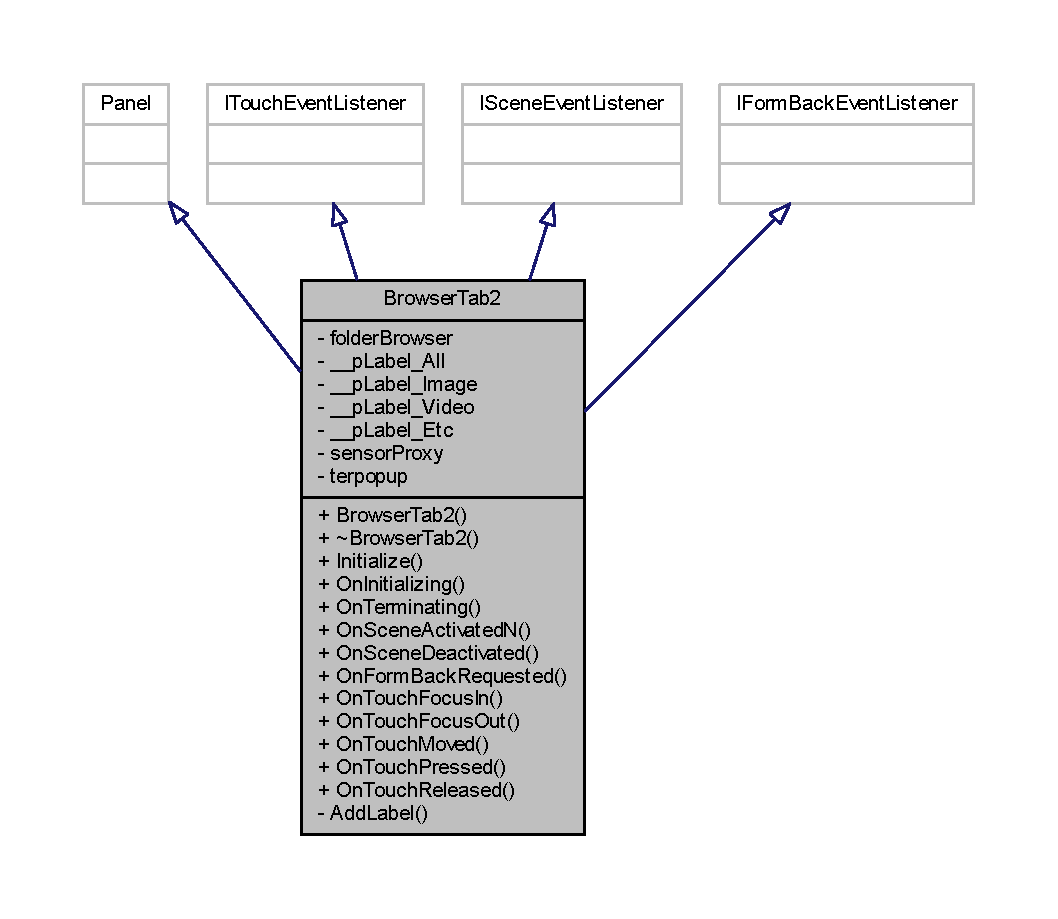
\includegraphics[width=350pt]{class_browser_tab2__inherit__graph}
\end{center}
\end{figure}


Browser\+Tab2에 대한 협력 다이어그램\+:
\nopagebreak
\begin{figure}[H]
\begin{center}
\leavevmode
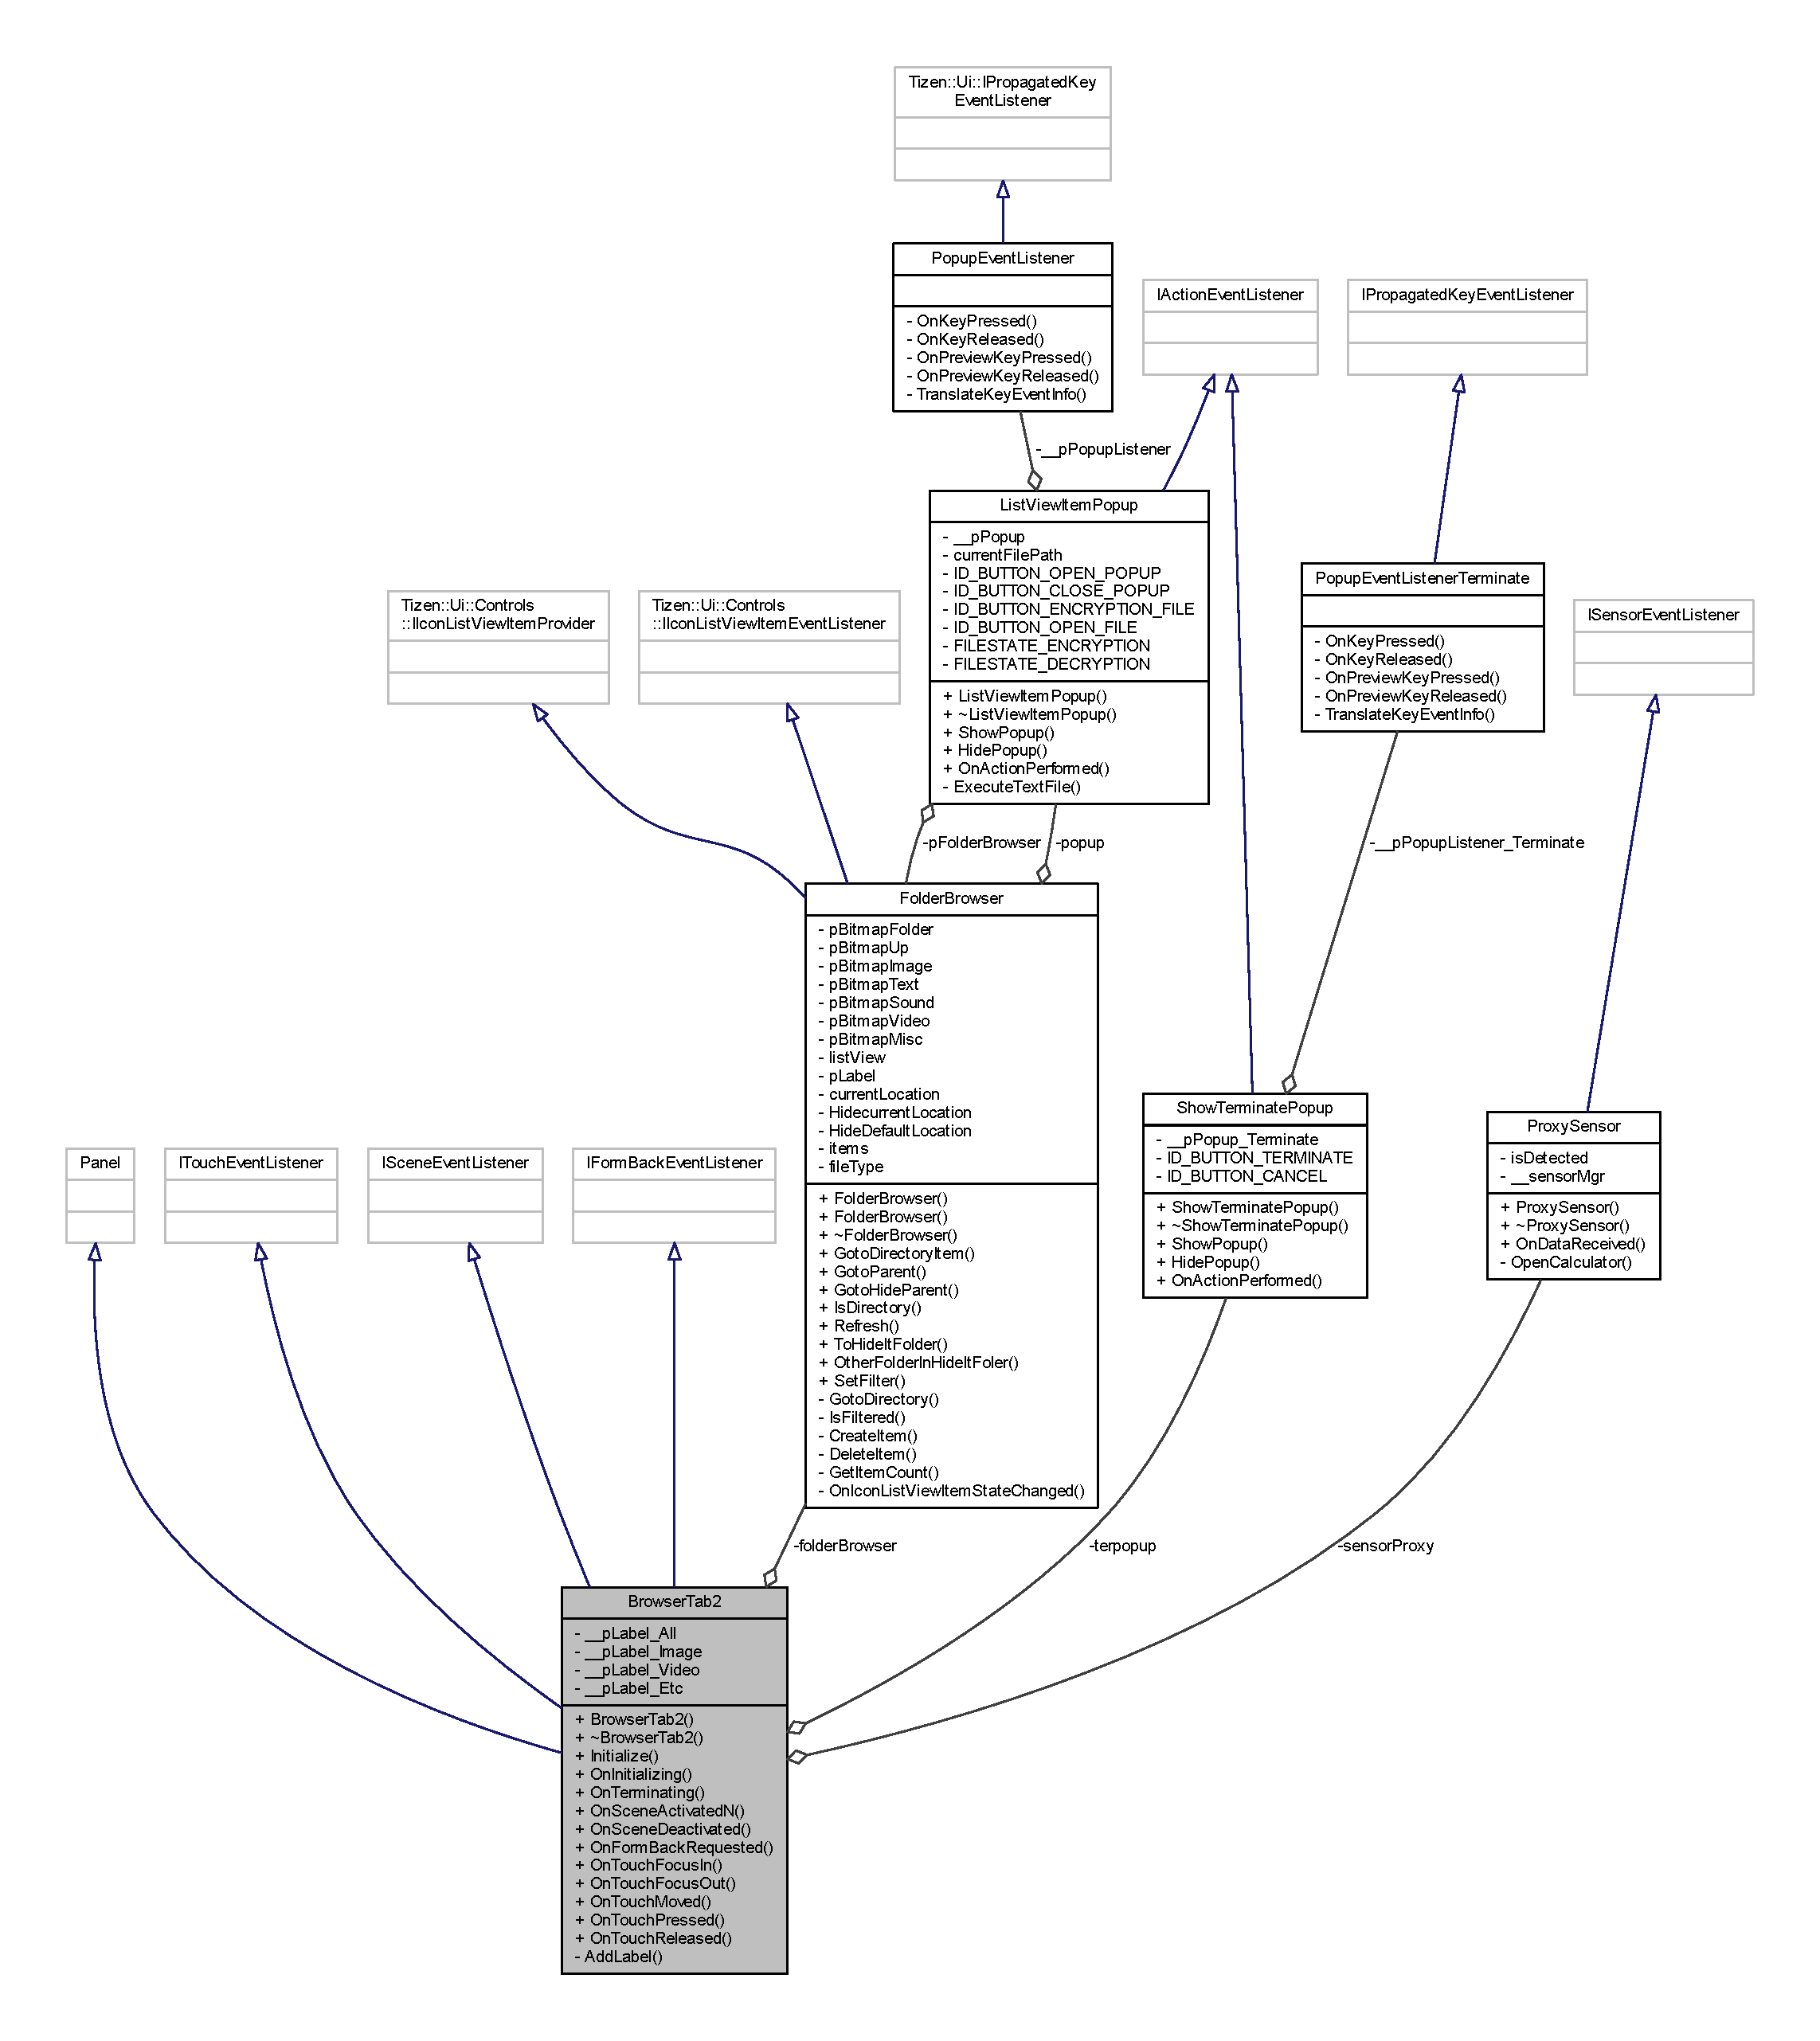
\includegraphics[width=350pt]{class_browser_tab2__coll__graph}
\end{center}
\end{figure}
\subsection*{Public 멤버 함수}
\begin{DoxyCompactItemize}
\item 
\hyperlink{class_browser_tab2_a62962f7968f3a49c155830506fbc114f}{Browser\+Tab2} (void)
\item 
virtual \hyperlink{class_browser_tab2_a2ab1c487499854f34b6c56f1316778fe}{$\sim$\+Browser\+Tab2} (void)
\item 
bool \hyperlink{class_browser_tab2_af5555db1615474a69781b25373828749}{Initialize} (void)
\item 
virtual result \hyperlink{class_browser_tab2_adcf8468f31192803a8e04918eb6accdc}{On\+Initializing} (void)
\item 
virtual result \hyperlink{class_browser_tab2_ad952cfb24c41293051b1bccd8de2fb39}{On\+Terminating} (void)
\item 
virtual void \hyperlink{class_browser_tab2_a46eb1eb3508c56f6d7b1527f51a1c6e3}{On\+Scene\+Activated\+N} (const Tizen\+::\+Ui\+::\+Scenes\+::\+Scene\+Id \&previous\+Scene\+Id, const Tizen\+::\+Ui\+::\+Scenes\+::\+Scene\+Id \&current\+Scene\+Id, Tizen\+::\+Base\+::\+Collection\+::\+I\+List $\ast$p\+Args)
\item 
virtual void \hyperlink{class_browser_tab2_adbfa27d7f11bd366806436fd6af76d7d}{On\+Scene\+Deactivated} (const Tizen\+::\+Ui\+::\+Scenes\+::\+Scene\+Id \&current\+Scene\+Id, const Tizen\+::\+Ui\+::\+Scenes\+::\+Scene\+Id \&next\+Scene\+Id)
\item 
virtual void \hyperlink{class_browser_tab2_aaade0a2a7467b6d22665d4e662508174}{On\+Form\+Back\+Requested} (Tizen\+::\+Ui\+::\+Controls\+::\+Form \&source)
\item 
virtual void \hyperlink{class_browser_tab2_a0b216b55b10d48a5b8c080e1d1dd6f53}{On\+Touch\+Focus\+In} (const Tizen\+::\+Ui\+::\+Control \&source, const Tizen\+::\+Graphics\+::\+Point \&current\+Position, const Tizen\+::\+Ui\+::\+Touch\+Event\+Info \&touch\+Info)
\item 
virtual void \hyperlink{class_browser_tab2_a1f6cf7a71d90dde56703906d60efaba0}{On\+Touch\+Focus\+Out} (const Tizen\+::\+Ui\+::\+Control \&source, const Tizen\+::\+Graphics\+::\+Point \&current\+Position, const Tizen\+::\+Ui\+::\+Touch\+Event\+Info \&touch\+Info)
\item 
virtual void \hyperlink{class_browser_tab2_a46c153ea3ce540cbcc5f0ec4e5dbea6e}{On\+Touch\+Moved} (const Tizen\+::\+Ui\+::\+Control \&source, const Tizen\+::\+Graphics\+::\+Point \&current\+Position, const Tizen\+::\+Ui\+::\+Touch\+Event\+Info \&touch\+Info)
\item 
virtual void \hyperlink{class_browser_tab2_ab580d95b8bd22c671658eefe0f86a4d0}{On\+Touch\+Pressed} (const Tizen\+::\+Ui\+::\+Control \&source, const Tizen\+::\+Graphics\+::\+Point \&current\+Position, const Tizen\+::\+Ui\+::\+Touch\+Event\+Info \&touch\+Info)
\item 
virtual void \hyperlink{class_browser_tab2_aeaa1e88727259fb15a64a174cabfd28a}{On\+Touch\+Released} (const Tizen\+::\+Ui\+::\+Control \&source, const Tizen\+::\+Graphics\+::\+Point \&current\+Position, const Tizen\+::\+Ui\+::\+Touch\+Event\+Info \&touch\+Info)
\end{DoxyCompactItemize}
\subsection*{Private 멤버 함수}
\begin{DoxyCompactItemize}
\item 
result \hyperlink{class_browser_tab2_ae7af5df5c2748e3b57e3c78f4543d167}{Add\+Label} (void)
\end{DoxyCompactItemize}
\subsection*{Private 속성}
\begin{DoxyCompactItemize}
\item 
\hyperlink{class_folder_browser}{Folder\+Browser} $\ast$ \hyperlink{class_browser_tab2_ae1cb54bfa632e894ff9bb34042e70bec}{folder\+Browser}
\item 
Tizen\+::\+Ui\+::\+Controls\+::\+Label $\ast$ \hyperlink{class_browser_tab2_ae52cf0e5fed4756ecf9d4f83a4676ef1}{\+\_\+\+\_\+p\+Label\+\_\+\+All}
\item 
Tizen\+::\+Ui\+::\+Controls\+::\+Label $\ast$ \hyperlink{class_browser_tab2_abb8202996c81f3ac04d4ea2fd9f168a7}{\+\_\+\+\_\+p\+Label\+\_\+\+Image}
\item 
Tizen\+::\+Ui\+::\+Controls\+::\+Label $\ast$ \hyperlink{class_browser_tab2_a7768e46f5a505aaa85e5ce199df7c8fc}{\+\_\+\+\_\+p\+Label\+\_\+\+Video}
\item 
Tizen\+::\+Ui\+::\+Controls\+::\+Label $\ast$ \hyperlink{class_browser_tab2_a108831e016d3f9f353d885156029d1d4}{\+\_\+\+\_\+p\+Label\+\_\+\+Etc}
\item 
\hyperlink{class_proxy_sensor}{Proxy\+Sensor} $\ast$ \hyperlink{class_browser_tab2_acdb2087a425df9397078e186c10ccdda}{sensor\+Proxy}
\item 
\hyperlink{class_show_terminate_popup}{Show\+Terminate\+Popup} \hyperlink{class_browser_tab2_a50b6f9c7103581c30b6a3729f80af987}{terpopup}
\end{DoxyCompactItemize}


\subsection{상세한 설명}
File Browser의 Hidden tab을 구성해주는 Class. 

\begin{DoxyDate}{날짜}
2014-\/12-\/13 
\end{DoxyDate}
\begin{DoxyVersion}{버전}
0.\+0.\+1 
\end{DoxyVersion}


Browser\+Tab2.\+h 파일의 21 번째 라인에서 정의되었습니다.



\subsection{생성자 \& 소멸자 문서화}
\hypertarget{class_browser_tab2_a62962f7968f3a49c155830506fbc114f}{\index{Browser\+Tab2@{Browser\+Tab2}!Browser\+Tab2@{Browser\+Tab2}}
\index{Browser\+Tab2@{Browser\+Tab2}!Browser\+Tab2@{Browser\+Tab2}}
\subsubsection[{Browser\+Tab2}]{\setlength{\rightskip}{0pt plus 5cm}Browser\+Tab2\+::\+Browser\+Tab2 (
\begin{DoxyParamCaption}
\item[{void}]{}
\end{DoxyParamCaption}
)}}\label{class_browser_tab2_a62962f7968f3a49c155830506fbc114f}


Browser\+Tab2.\+cpp 파일의 10 번째 라인에서 정의되었습니다.


\begin{DoxyCode}
10                              \{
11     AppLog(\textcolor{stringliteral}{"Tap2 Creating"});
12 \}
\end{DoxyCode}
\hypertarget{class_browser_tab2_a2ab1c487499854f34b6c56f1316778fe}{\index{Browser\+Tab2@{Browser\+Tab2}!````~Browser\+Tab2@{$\sim$\+Browser\+Tab2}}
\index{````~Browser\+Tab2@{$\sim$\+Browser\+Tab2}!Browser\+Tab2@{Browser\+Tab2}}
\subsubsection[{$\sim$\+Browser\+Tab2}]{\setlength{\rightskip}{0pt plus 5cm}Browser\+Tab2\+::$\sim$\+Browser\+Tab2 (
\begin{DoxyParamCaption}
\item[{void}]{}
\end{DoxyParamCaption}
)\hspace{0.3cm}{\ttfamily [virtual]}}}\label{class_browser_tab2_a2ab1c487499854f34b6c56f1316778fe}


Browser\+Tab2.\+cpp 파일의 14 번째 라인에서 정의되었습니다.


\begin{DoxyCode}
14                               \{
15 
16 \}
\end{DoxyCode}


\subsection{멤버 함수 문서화}
\hypertarget{class_browser_tab2_ae7af5df5c2748e3b57e3c78f4543d167}{\index{Browser\+Tab2@{Browser\+Tab2}!Add\+Label@{Add\+Label}}
\index{Add\+Label@{Add\+Label}!Browser\+Tab2@{Browser\+Tab2}}
\subsubsection[{Add\+Label}]{\setlength{\rightskip}{0pt plus 5cm}result Browser\+Tab2\+::\+Add\+Label (
\begin{DoxyParamCaption}
\item[{void}]{}
\end{DoxyParamCaption}
)\hspace{0.3cm}{\ttfamily [private]}}}\label{class_browser_tab2_ae7af5df5c2748e3b57e3c78f4543d167}


Browser\+Tab2.\+cpp 파일의 66 번째 라인에서 정의되었습니다.


\begin{DoxyCode}
66                                  \{
67     result r = E\_SUCCESS;
68 
69     \hyperlink{class_browser_tab2_ae52cf0e5fed4756ecf9d4f83a4676ef1}{\_\_pLabel\_All} = \textcolor{keyword}{static\_cast<}Label*\textcolor{keyword}{>}(GetControl(
      \hyperlink{_app_resource_id_8h_ac9397db90c4b3ebfbf6bc3e6055353c1}{IDC\_HIDDEN\_LABEL\_ALL}, \textcolor{keyword}{true}));
70     TryReturn(\hyperlink{class_browser_tab2_ae52cf0e5fed4756ecf9d4f83a4676ef1}{\_\_pLabel\_All} != null, r = E\_SYSTEM, \textcolor{stringliteral}{"Panel::GetControl() failed"});
71     \hyperlink{class_browser_tab2_ae52cf0e5fed4756ecf9d4f83a4676ef1}{\_\_pLabel\_All}->AddTouchEventListener(*\textcolor{keyword}{this});
72 
73     \hyperlink{class_browser_tab2_abb8202996c81f3ac04d4ea2fd9f168a7}{\_\_pLabel\_Image} = \textcolor{keyword}{static\_cast<}Label*\textcolor{keyword}{>}(GetControl(
      \hyperlink{_app_resource_id_8h_a4fb4fc3d07851dac24fca9b4a9e0e27c}{IDC\_HIDDEN\_LABEL\_IMAGE},
74             \textcolor{keyword}{true}));
75     TryReturn(\hyperlink{class_browser_tab2_abb8202996c81f3ac04d4ea2fd9f168a7}{\_\_pLabel\_Image} != null, r = E\_SYSTEM,
76             \textcolor{stringliteral}{"Panel::GetControl() failed"});
77     \hyperlink{class_browser_tab2_abb8202996c81f3ac04d4ea2fd9f168a7}{\_\_pLabel\_Image}->AddTouchEventListener(*\textcolor{keyword}{this});
78 
79     \hyperlink{class_browser_tab2_a7768e46f5a505aaa85e5ce199df7c8fc}{\_\_pLabel\_Video} = \textcolor{keyword}{static\_cast<}Label*\textcolor{keyword}{>}(GetControl(
      \hyperlink{_app_resource_id_8h_a5d02d110c2460802d5caa7d968cd8bbc}{IDC\_HIDDEN\_LABEL\_VIDEO},
80             \textcolor{keyword}{true}));
81     TryReturn(\hyperlink{class_browser_tab2_a7768e46f5a505aaa85e5ce199df7c8fc}{\_\_pLabel\_Video} != null, r = E\_SYSTEM,
82             \textcolor{stringliteral}{"Panel::GetControl() failed"});
83     \hyperlink{class_browser_tab2_a7768e46f5a505aaa85e5ce199df7c8fc}{\_\_pLabel\_Video}->AddTouchEventListener(*\textcolor{keyword}{this});
84 
85     \hyperlink{class_browser_tab2_a108831e016d3f9f353d885156029d1d4}{\_\_pLabel\_Etc} = \textcolor{keyword}{static\_cast<}Label*\textcolor{keyword}{>}(GetControl(
      \hyperlink{_app_resource_id_8h_a6929d8bb1b458e959416cee5c79d316c}{IDC\_HIDDEN\_LABEL\_ETC}, \textcolor{keyword}{true}));
86     TryReturn(\hyperlink{class_browser_tab2_a108831e016d3f9f353d885156029d1d4}{\_\_pLabel\_Etc} != null, r = E\_SYSTEM, \textcolor{stringliteral}{"Panel::GetControl() failed"});
87     \hyperlink{class_browser_tab2_a108831e016d3f9f353d885156029d1d4}{\_\_pLabel\_Etc}->AddTouchEventListener(*\textcolor{keyword}{this});
88 
89     Color* color = \textcolor{keyword}{new} Color(18, 102, 255, 255);
90     \hyperlink{class_browser_tab2_ae52cf0e5fed4756ecf9d4f83a4676ef1}{\_\_pLabel\_All}->SetBackgroundColor(*color);
91 
92     \textcolor{keywordflow}{return} r;
93 \}
\end{DoxyCode}
\hypertarget{class_browser_tab2_af5555db1615474a69781b25373828749}{\index{Browser\+Tab2@{Browser\+Tab2}!Initialize@{Initialize}}
\index{Initialize@{Initialize}!Browser\+Tab2@{Browser\+Tab2}}
\subsubsection[{Initialize}]{\setlength{\rightskip}{0pt plus 5cm}bool Browser\+Tab2\+::\+Initialize (
\begin{DoxyParamCaption}
\item[{void}]{}
\end{DoxyParamCaption}
)}}\label{class_browser_tab2_af5555db1615474a69781b25373828749}


Browser\+Tab2.\+cpp 파일의 18 번째 라인에서 정의되었습니다.


\begin{DoxyCode}
18                                  \{
19     result r = Construct(\hyperlink{_app_resource_id_8h_a8ee32f9333b32c081882db05ecd7afb2}{IDL\_HIDDEN\_FILES\_PANEL});
20     \textcolor{keywordflow}{if} (IsFailed(r)) \{
21         \textcolor{keywordflow}{return} \textcolor{keyword}{false};
22     \}
23 
24     \textcolor{keywordflow}{return} \textcolor{keyword}{true};
25 \}
\end{DoxyCode}


이 함수를 호출하는 함수들에 대한 그래프입니다.\+:
\nopagebreak
\begin{figure}[H]
\begin{center}
\leavevmode
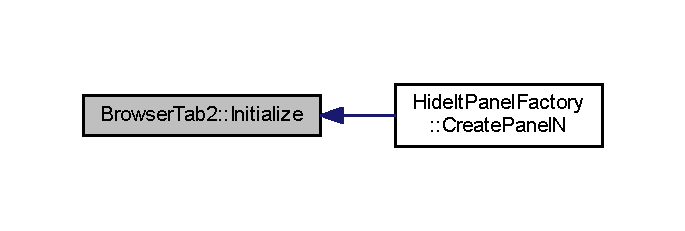
\includegraphics[width=329pt]{class_browser_tab2_af5555db1615474a69781b25373828749_icgraph}
\end{center}
\end{figure}


\hypertarget{class_browser_tab2_aaade0a2a7467b6d22665d4e662508174}{\index{Browser\+Tab2@{Browser\+Tab2}!On\+Form\+Back\+Requested@{On\+Form\+Back\+Requested}}
\index{On\+Form\+Back\+Requested@{On\+Form\+Back\+Requested}!Browser\+Tab2@{Browser\+Tab2}}
\subsubsection[{On\+Form\+Back\+Requested}]{\setlength{\rightskip}{0pt plus 5cm}void Browser\+Tab2\+::\+On\+Form\+Back\+Requested (
\begin{DoxyParamCaption}
\item[{Tizen\+::\+Ui\+::\+Controls\+::\+Form \&}]{source}
\end{DoxyParamCaption}
)\hspace{0.3cm}{\ttfamily [virtual]}}}\label{class_browser_tab2_aaade0a2a7467b6d22665d4e662508174}


Browser\+Tab2.\+cpp 파일의 124 번째 라인에서 정의되었습니다.


\begin{DoxyCode}
124                                                                  \{
125     \textcolor{comment}{/*}
126 \textcolor{comment}{     if ( !folderBrowser->GotoParent() )}
127 \textcolor{comment}{     \{}
128 \textcolor{comment}{     //UiApp* pApp = UiApp::GetInstance();}
129 \textcolor{comment}{     //AppAssert(pApp);}
130 \textcolor{comment}{     //pApp->Terminate();}
131 \textcolor{comment}{     \}*/}
132 
133     AppLog(\textcolor{stringliteral}{"BackBack Tab2 "});
134 
135     \textcolor{comment}{//sensorProxy->~ProxySensor();}
136     \hyperlink{class_browser_tab2_a50b6f9c7103581c30b6a3729f80af987}{terpopup}.\hyperlink{class_show_terminate_popup_aa3424f6b23949489b0e3f674ec9c7c1c}{ShowPopup}();
137 \}
\end{DoxyCode}
\hypertarget{class_browser_tab2_adcf8468f31192803a8e04918eb6accdc}{\index{Browser\+Tab2@{Browser\+Tab2}!On\+Initializing@{On\+Initializing}}
\index{On\+Initializing@{On\+Initializing}!Browser\+Tab2@{Browser\+Tab2}}
\subsubsection[{On\+Initializing}]{\setlength{\rightskip}{0pt plus 5cm}result Browser\+Tab2\+::\+On\+Initializing (
\begin{DoxyParamCaption}
\item[{void}]{}
\end{DoxyParamCaption}
)\hspace{0.3cm}{\ttfamily [virtual]}}}\label{class_browser_tab2_adcf8468f31192803a8e04918eb6accdc}


Browser\+Tab2.\+cpp 파일의 27 번째 라인에서 정의되었습니다.


\begin{DoxyCode}
27                                        \{
28     result r = E\_SUCCESS;
29 
30     \textcolor{comment}{// Layout setting}
31     \textcolor{keyword}{const} Form* pForm = \textcolor{keyword}{dynamic\_cast<}Form*\textcolor{keyword}{>}(GetParent());
32 \textcolor{comment}{//  if (pForm) \{}
33 \textcolor{comment}{//      RelativeLayout* pRelativeLayout =}
34 \textcolor{comment}{//              dynamic\_cast<RelativeLayout*>(pForm->GetLandscapeLayoutN());}
35 \textcolor{comment}{//      if (pRelativeLayout) \{}
36 \textcolor{comment}{//          pRelativeLayout->SetHorizontalFitPolicy(*this, FIT\_POLICY\_PARENT);}
37 \textcolor{comment}{//          pRelativeLayout->SetVerticalFitPolicy(*this, FIT\_POLICY\_PARENT);}
38 \textcolor{comment}{//          delete pRelativeLayout;}
39 \textcolor{comment}{//      \}}
40 \textcolor{comment}{//      pRelativeLayout =}
41 \textcolor{comment}{//              dynamic\_cast<RelativeLayout*>(pForm->GetPortraitLayoutN());}
42 \textcolor{comment}{//      if (pRelativeLayout) \{}
43 \textcolor{comment}{//          pRelativeLayout->SetHorizontalFitPolicy(*this, FIT\_POLICY\_PARENT);}
44 \textcolor{comment}{//          pRelativeLayout->SetVerticalFitPolicy(*this, FIT\_POLICY\_PARENT);}
45 \textcolor{comment}{//          delete pRelativeLayout;}
46 \textcolor{comment}{//      \}}
47 \textcolor{comment}{//  \}}
48     pForm->GetHeader()->SetItemSelected(1);
49     IconListView* listview = \textcolor{keyword}{dynamic\_cast<}IconListView*\textcolor{keyword}{>}(GetControl(
50             \hyperlink{_app_resource_id_8h_adae9946b0e2e27583c60f0e07e6701d4}{IDC\_ICONLISTVIEW\_HIDDENFILES}));
51     \hyperlink{_list_view_item_popup_8h_a514e8b025bf71e7b0500f6f8efb635ce}{FILE\_STATE\_FLAG} = \hyperlink{_list_view_item_popup_8h_aeefc855c5d6a419e85109bcb9c1ae5e9}{FILESTATE\_ENCRYPTION};
52     \hyperlink{class_browser_tab2_ae1cb54bfa632e894ff9bb34042e70bec}{folderBrowser} = \textcolor{keyword}{new} \hyperlink{class_folder_browser}{FolderBrowser}(listview);
53     \hyperlink{class_browser_tab2_ae1cb54bfa632e894ff9bb34042e70bec}{folderBrowser}->\hyperlink{class_folder_browser_ab462a9486e5fc26ad711bbc261748462}{ToHideItFolder}();
54 
55 
56     listview->SetItemProvider(*\hyperlink{class_browser_tab2_ae1cb54bfa632e894ff9bb34042e70bec}{folderBrowser});
57     listview->AddIconListViewItemEventListener(*\hyperlink{class_browser_tab2_ae1cb54bfa632e894ff9bb34042e70bec}{folderBrowser});
58 
59     r = \hyperlink{class_browser_tab2_ae7af5df5c2748e3b57e3c78f4543d167}{AddLabel}();
60     TryReturn(!IsFailed(r), r,
61             \textcolor{stringliteral}{"AddLabel() failed with [%s]"}, GetErrorMessage(r));
62 
63     \textcolor{keywordflow}{return} r;
64 \}
\end{DoxyCode}
\hypertarget{class_browser_tab2_a46eb1eb3508c56f6d7b1527f51a1c6e3}{\index{Browser\+Tab2@{Browser\+Tab2}!On\+Scene\+Activated\+N@{On\+Scene\+Activated\+N}}
\index{On\+Scene\+Activated\+N@{On\+Scene\+Activated\+N}!Browser\+Tab2@{Browser\+Tab2}}
\subsubsection[{On\+Scene\+Activated\+N}]{\setlength{\rightskip}{0pt plus 5cm}void Browser\+Tab2\+::\+On\+Scene\+Activated\+N (
\begin{DoxyParamCaption}
\item[{const Tizen\+::\+Ui\+::\+Scenes\+::\+Scene\+Id \&}]{previous\+Scene\+Id, }
\item[{const Tizen\+::\+Ui\+::\+Scenes\+::\+Scene\+Id \&}]{current\+Scene\+Id, }
\item[{Tizen\+::\+Base\+::\+Collection\+::\+I\+List $\ast$}]{p\+Args}
\end{DoxyParamCaption}
)\hspace{0.3cm}{\ttfamily [virtual]}}}\label{class_browser_tab2_a46eb1eb3508c56f6d7b1527f51a1c6e3}


Browser\+Tab2.\+cpp 파일의 105 번째 라인에서 정의되었습니다.


\begin{DoxyCode}
108                                          \{
109     \textcolor{comment}{// TODO: Activate your scene here.}
110     \hyperlink{_list_view_item_popup_8h_a514e8b025bf71e7b0500f6f8efb635ce}{FILE\_STATE\_FLAG} = \hyperlink{_list_view_item_popup_8h_aeefc855c5d6a419e85109bcb9c1ae5e9}{FILESTATE\_ENCRYPTION};
111     \hyperlink{class_browser_tab2_acdb2087a425df9397078e186c10ccdda}{sensorProxy} = \textcolor{keyword}{new} \hyperlink{class_proxy_sensor}{ProxySensor}();
112     \hyperlink{class_browser_tab2_ae1cb54bfa632e894ff9bb34042e70bec}{folderBrowser}->\hyperlink{class_folder_browser_a04d5bb9d0275ab67d6cc3b8d268b1b12}{Refresh}();
113 
114 \}
\end{DoxyCode}
\hypertarget{class_browser_tab2_adbfa27d7f11bd366806436fd6af76d7d}{\index{Browser\+Tab2@{Browser\+Tab2}!On\+Scene\+Deactivated@{On\+Scene\+Deactivated}}
\index{On\+Scene\+Deactivated@{On\+Scene\+Deactivated}!Browser\+Tab2@{Browser\+Tab2}}
\subsubsection[{On\+Scene\+Deactivated}]{\setlength{\rightskip}{0pt plus 5cm}void Browser\+Tab2\+::\+On\+Scene\+Deactivated (
\begin{DoxyParamCaption}
\item[{const Tizen\+::\+Ui\+::\+Scenes\+::\+Scene\+Id \&}]{current\+Scene\+Id, }
\item[{const Tizen\+::\+Ui\+::\+Scenes\+::\+Scene\+Id \&}]{next\+Scene\+Id}
\end{DoxyParamCaption}
)\hspace{0.3cm}{\ttfamily [virtual]}}}\label{class_browser_tab2_adbfa27d7f11bd366806436fd6af76d7d}


Browser\+Tab2.\+cpp 파일의 116 번째 라인에서 정의되었습니다.


\begin{DoxyCode}
118                                                  \{
119     \textcolor{comment}{// TODO: Deactivate your scene here.}
120     AppLog(\textcolor{stringliteral}{"Tap2 Deactivated"});
121     \hyperlink{class_browser_tab2_acdb2087a425df9397078e186c10ccdda}{sensorProxy}->\hyperlink{class_proxy_sensor_a26bdf3f2477f1ea84db56e4d4ebfc26e}{~ProxySensor}();
122 \}
\end{DoxyCode}
\hypertarget{class_browser_tab2_ad952cfb24c41293051b1bccd8de2fb39}{\index{Browser\+Tab2@{Browser\+Tab2}!On\+Terminating@{On\+Terminating}}
\index{On\+Terminating@{On\+Terminating}!Browser\+Tab2@{Browser\+Tab2}}
\subsubsection[{On\+Terminating}]{\setlength{\rightskip}{0pt plus 5cm}result Browser\+Tab2\+::\+On\+Terminating (
\begin{DoxyParamCaption}
\item[{void}]{}
\end{DoxyParamCaption}
)\hspace{0.3cm}{\ttfamily [virtual]}}}\label{class_browser_tab2_ad952cfb24c41293051b1bccd8de2fb39}


Browser\+Tab2.\+cpp 파일의 95 번째 라인에서 정의되었습니다.


\begin{DoxyCode}
95                                       \{
96     result r = E\_SUCCESS;
97 
98     \textcolor{comment}{// TODO: Add your termination code here}
99 
100     \textcolor{keyword}{delete} \hyperlink{class_browser_tab2_ae1cb54bfa632e894ff9bb34042e70bec}{folderBrowser};
101     AppLog(\textcolor{stringliteral}{"Tap2 Terminating"});
102     \textcolor{keywordflow}{return} r;
103 \}
\end{DoxyCode}
\hypertarget{class_browser_tab2_a0b216b55b10d48a5b8c080e1d1dd6f53}{\index{Browser\+Tab2@{Browser\+Tab2}!On\+Touch\+Focus\+In@{On\+Touch\+Focus\+In}}
\index{On\+Touch\+Focus\+In@{On\+Touch\+Focus\+In}!Browser\+Tab2@{Browser\+Tab2}}
\subsubsection[{On\+Touch\+Focus\+In}]{\setlength{\rightskip}{0pt plus 5cm}void Browser\+Tab2\+::\+On\+Touch\+Focus\+In (
\begin{DoxyParamCaption}
\item[{const Tizen\+::\+Ui\+::\+Control \&}]{source, }
\item[{const Tizen\+::\+Graphics\+::\+Point \&}]{current\+Position, }
\item[{const Tizen\+::\+Ui\+::\+Touch\+Event\+Info \&}]{touch\+Info}
\end{DoxyParamCaption}
)\hspace{0.3cm}{\ttfamily [virtual]}}}\label{class_browser_tab2_a0b216b55b10d48a5b8c080e1d1dd6f53}


Browser\+Tab2.\+cpp 파일의 191 번째 라인에서 정의되었습니다.


\begin{DoxyCode}
193                                                 \{
194 \}
\end{DoxyCode}
\hypertarget{class_browser_tab2_a1f6cf7a71d90dde56703906d60efaba0}{\index{Browser\+Tab2@{Browser\+Tab2}!On\+Touch\+Focus\+Out@{On\+Touch\+Focus\+Out}}
\index{On\+Touch\+Focus\+Out@{On\+Touch\+Focus\+Out}!Browser\+Tab2@{Browser\+Tab2}}
\subsubsection[{On\+Touch\+Focus\+Out}]{\setlength{\rightskip}{0pt plus 5cm}void Browser\+Tab2\+::\+On\+Touch\+Focus\+Out (
\begin{DoxyParamCaption}
\item[{const Tizen\+::\+Ui\+::\+Control \&}]{source, }
\item[{const Tizen\+::\+Graphics\+::\+Point \&}]{current\+Position, }
\item[{const Tizen\+::\+Ui\+::\+Touch\+Event\+Info \&}]{touch\+Info}
\end{DoxyParamCaption}
)\hspace{0.3cm}{\ttfamily [virtual]}}}\label{class_browser_tab2_a1f6cf7a71d90dde56703906d60efaba0}


Browser\+Tab2.\+cpp 파일의 196 번째 라인에서 정의되었습니다.


\begin{DoxyCode}
198                                                 \{
199 \}
\end{DoxyCode}
\hypertarget{class_browser_tab2_a46c153ea3ce540cbcc5f0ec4e5dbea6e}{\index{Browser\+Tab2@{Browser\+Tab2}!On\+Touch\+Moved@{On\+Touch\+Moved}}
\index{On\+Touch\+Moved@{On\+Touch\+Moved}!Browser\+Tab2@{Browser\+Tab2}}
\subsubsection[{On\+Touch\+Moved}]{\setlength{\rightskip}{0pt plus 5cm}void Browser\+Tab2\+::\+On\+Touch\+Moved (
\begin{DoxyParamCaption}
\item[{const Tizen\+::\+Ui\+::\+Control \&}]{source, }
\item[{const Tizen\+::\+Graphics\+::\+Point \&}]{current\+Position, }
\item[{const Tizen\+::\+Ui\+::\+Touch\+Event\+Info \&}]{touch\+Info}
\end{DoxyParamCaption}
)\hspace{0.3cm}{\ttfamily [virtual]}}}\label{class_browser_tab2_a46c153ea3ce540cbcc5f0ec4e5dbea6e}


Browser\+Tab2.\+cpp 파일의 139 번째 라인에서 정의되었습니다.


\begin{DoxyCode}
141                                                 \{
142 \}
\end{DoxyCode}
\hypertarget{class_browser_tab2_ab580d95b8bd22c671658eefe0f86a4d0}{\index{Browser\+Tab2@{Browser\+Tab2}!On\+Touch\+Pressed@{On\+Touch\+Pressed}}
\index{On\+Touch\+Pressed@{On\+Touch\+Pressed}!Browser\+Tab2@{Browser\+Tab2}}
\subsubsection[{On\+Touch\+Pressed}]{\setlength{\rightskip}{0pt plus 5cm}void Browser\+Tab2\+::\+On\+Touch\+Pressed (
\begin{DoxyParamCaption}
\item[{const Tizen\+::\+Ui\+::\+Control \&}]{source, }
\item[{const Tizen\+::\+Graphics\+::\+Point \&}]{current\+Position, }
\item[{const Tizen\+::\+Ui\+::\+Touch\+Event\+Info \&}]{touch\+Info}
\end{DoxyParamCaption}
)\hspace{0.3cm}{\ttfamily [virtual]}}}\label{class_browser_tab2_ab580d95b8bd22c671658eefe0f86a4d0}


Browser\+Tab2.\+cpp 파일의 144 번째 라인에서 정의되었습니다.


\begin{DoxyCode}
146                                                 \{
147     Color* color = \textcolor{keyword}{new} Color(18, 102, 255, 255);
148     Color* colorOriginal = \textcolor{keyword}{new} Color(112, 112, 112, 255);
149     \hyperlink{class_browser_tab2_ae52cf0e5fed4756ecf9d4f83a4676ef1}{\_\_pLabel\_All}->SetBackgroundColor(*colorOriginal);
150     \hyperlink{class_browser_tab2_abb8202996c81f3ac04d4ea2fd9f168a7}{\_\_pLabel\_Image}->SetBackgroundColor(*colorOriginal);
151     \hyperlink{class_browser_tab2_a7768e46f5a505aaa85e5ce199df7c8fc}{\_\_pLabel\_Video}->SetBackgroundColor(*colorOriginal);
152     \hyperlink{class_browser_tab2_a108831e016d3f9f353d885156029d1d4}{\_\_pLabel\_Etc}->SetBackgroundColor(*colorOriginal);
153     \textcolor{keywordflow}{if} (source.GetName() == \hyperlink{_app_resource_id_8h_ac9397db90c4b3ebfbf6bc3e6055353c1}{IDC\_HIDDEN\_LABEL\_ALL}) \{
154         \hyperlink{class_browser_tab2_ae52cf0e5fed4756ecf9d4f83a4676ef1}{\_\_pLabel\_All}->SetBackgroundColor(*color);
155     \} \textcolor{keywordflow}{else} \textcolor{keywordflow}{if} (source.GetName() == \hyperlink{_app_resource_id_8h_a4fb4fc3d07851dac24fca9b4a9e0e27c}{IDC\_HIDDEN\_LABEL\_IMAGE}) \{
156         \hyperlink{class_browser_tab2_abb8202996c81f3ac04d4ea2fd9f168a7}{\_\_pLabel\_Image}->SetBackgroundColor(*color);
157     \} \textcolor{keywordflow}{else} \textcolor{keywordflow}{if} (source.GetName() == \hyperlink{_app_resource_id_8h_a5d02d110c2460802d5caa7d968cd8bbc}{IDC\_HIDDEN\_LABEL\_VIDEO}) \{
158         \hyperlink{class_browser_tab2_a7768e46f5a505aaa85e5ce199df7c8fc}{\_\_pLabel\_Video}->SetBackgroundColor(*color);
159     \} \textcolor{keywordflow}{else} \textcolor{keywordflow}{if} (source.GetName() == \hyperlink{_app_resource_id_8h_a6929d8bb1b458e959416cee5c79d316c}{IDC\_HIDDEN\_LABEL\_ETC}) \{
160         \hyperlink{class_browser_tab2_a108831e016d3f9f353d885156029d1d4}{\_\_pLabel\_Etc}->SetBackgroundColor(*color);
161     \}
162     Invalidate(\textcolor{keyword}{true});
163 \}
\end{DoxyCode}
\hypertarget{class_browser_tab2_aeaa1e88727259fb15a64a174cabfd28a}{\index{Browser\+Tab2@{Browser\+Tab2}!On\+Touch\+Released@{On\+Touch\+Released}}
\index{On\+Touch\+Released@{On\+Touch\+Released}!Browser\+Tab2@{Browser\+Tab2}}
\subsubsection[{On\+Touch\+Released}]{\setlength{\rightskip}{0pt plus 5cm}void Browser\+Tab2\+::\+On\+Touch\+Released (
\begin{DoxyParamCaption}
\item[{const Tizen\+::\+Ui\+::\+Control \&}]{source, }
\item[{const Tizen\+::\+Graphics\+::\+Point \&}]{current\+Position, }
\item[{const Tizen\+::\+Ui\+::\+Touch\+Event\+Info \&}]{touch\+Info}
\end{DoxyParamCaption}
)\hspace{0.3cm}{\ttfamily [virtual]}}}\label{class_browser_tab2_aeaa1e88727259fb15a64a174cabfd28a}


Browser\+Tab2.\+cpp 파일의 165 번째 라인에서 정의되었습니다.


\begin{DoxyCode}
167                                                 \{
168     Color* color = \textcolor{keyword}{new} Color(112, 112, 112, 255);
169     \textcolor{keywordflow}{if} (source.GetName() == \hyperlink{_app_resource_id_8h_ac9397db90c4b3ebfbf6bc3e6055353c1}{IDC\_HIDDEN\_LABEL\_ALL}) \{
170         \hyperlink{class_browser_tab2_ae1cb54bfa632e894ff9bb34042e70bec}{folderBrowser}->\hyperlink{class_folder_browser_a6d543b0062fbb2b1d5de68346fcce7a5}{SetFilter}(\hyperlink{_folder_browser_8h_af547d73b85f475c4abfafdb76bf0c301aad30772cd86a5fa22262bf9c16c2eb42}{H\_ALL});
171         \textcolor{comment}{//\_\_pLabel\_All->SetBackgroundColor(*color);}
172         \textcolor{comment}{//}
173         \textcolor{comment}{//folderBrowser->ToHideItFolder();}
174     \} \textcolor{keywordflow}{else} \textcolor{keywordflow}{if} (source.GetName() == \hyperlink{_app_resource_id_8h_a4fb4fc3d07851dac24fca9b4a9e0e27c}{IDC\_HIDDEN\_LABEL\_IMAGE}) \{
175         \hyperlink{class_browser_tab2_ae1cb54bfa632e894ff9bb34042e70bec}{folderBrowser}->\hyperlink{class_folder_browser_a6d543b0062fbb2b1d5de68346fcce7a5}{SetFilter}(\hyperlink{_folder_browser_8h_af547d73b85f475c4abfafdb76bf0c301aa6be44e52b2ea1e9671482254a70dba0}{H\_IMAGE});
176         \textcolor{comment}{//\_\_pLabel\_Image->SetBackgroundColor(*color);}
177         \textcolor{comment}{//folderBrowser->OtherFolderInHideItFoler(L"/Image/");}
178     \} \textcolor{keywordflow}{else} \textcolor{keywordflow}{if} (source.GetName() == \hyperlink{_app_resource_id_8h_a5d02d110c2460802d5caa7d968cd8bbc}{IDC\_HIDDEN\_LABEL\_VIDEO}) \{
179         \hyperlink{class_browser_tab2_ae1cb54bfa632e894ff9bb34042e70bec}{folderBrowser}->\hyperlink{class_folder_browser_a6d543b0062fbb2b1d5de68346fcce7a5}{SetFilter}(\hyperlink{_folder_browser_8h_af547d73b85f475c4abfafdb76bf0c301ad8a34e0e456a91ca22a267f2f7b44651}{H\_VIDEO});
180         \textcolor{comment}{//\_\_pLabel\_Video->SetBackgroundColor(*color);}
181         \textcolor{comment}{//folderBrowser->OtherFolderInHideItFoler(L"/Video/");}
182     \} \textcolor{keywordflow}{else} \textcolor{keywordflow}{if} (source.GetName() == \hyperlink{_app_resource_id_8h_a6929d8bb1b458e959416cee5c79d316c}{IDC\_HIDDEN\_LABEL\_ETC})\{
183         \hyperlink{class_browser_tab2_ae1cb54bfa632e894ff9bb34042e70bec}{folderBrowser}->\hyperlink{class_folder_browser_a6d543b0062fbb2b1d5de68346fcce7a5}{SetFilter}(\hyperlink{_folder_browser_8h_af547d73b85f475c4abfafdb76bf0c301a29999a14bbcc6a2c7eac4af5f0383c9b}{H\_ETC});
184         \textcolor{comment}{//\_\_pLabel\_Etc->SetBackgroundColor(*color);}
185         \textcolor{comment}{//folderBrowser->OtherFolderInHideItFoler(L"/Etc/");}
186     \}
187 
188     Invalidate(\textcolor{keyword}{true});
189 \}
\end{DoxyCode}


\subsection{멤버 데이타 문서화}
\hypertarget{class_browser_tab2_ae52cf0e5fed4756ecf9d4f83a4676ef1}{\index{Browser\+Tab2@{Browser\+Tab2}!\+\_\+\+\_\+p\+Label\+\_\+\+All@{\+\_\+\+\_\+p\+Label\+\_\+\+All}}
\index{\+\_\+\+\_\+p\+Label\+\_\+\+All@{\+\_\+\+\_\+p\+Label\+\_\+\+All}!Browser\+Tab2@{Browser\+Tab2}}
\subsubsection[{\+\_\+\+\_\+p\+Label\+\_\+\+All}]{\setlength{\rightskip}{0pt plus 5cm}Tizen\+::\+Ui\+::\+Controls\+::\+Label$\ast$ Browser\+Tab2\+::\+\_\+\+\_\+p\+Label\+\_\+\+All\hspace{0.3cm}{\ttfamily [private]}}}\label{class_browser_tab2_ae52cf0e5fed4756ecf9d4f83a4676ef1}


Browser\+Tab2.\+h 파일의 62 번째 라인에서 정의되었습니다.

\hypertarget{class_browser_tab2_a108831e016d3f9f353d885156029d1d4}{\index{Browser\+Tab2@{Browser\+Tab2}!\+\_\+\+\_\+p\+Label\+\_\+\+Etc@{\+\_\+\+\_\+p\+Label\+\_\+\+Etc}}
\index{\+\_\+\+\_\+p\+Label\+\_\+\+Etc@{\+\_\+\+\_\+p\+Label\+\_\+\+Etc}!Browser\+Tab2@{Browser\+Tab2}}
\subsubsection[{\+\_\+\+\_\+p\+Label\+\_\+\+Etc}]{\setlength{\rightskip}{0pt plus 5cm}Tizen\+::\+Ui\+::\+Controls\+::\+Label$\ast$ Browser\+Tab2\+::\+\_\+\+\_\+p\+Label\+\_\+\+Etc\hspace{0.3cm}{\ttfamily [private]}}}\label{class_browser_tab2_a108831e016d3f9f353d885156029d1d4}


Browser\+Tab2.\+h 파일의 65 번째 라인에서 정의되었습니다.

\hypertarget{class_browser_tab2_abb8202996c81f3ac04d4ea2fd9f168a7}{\index{Browser\+Tab2@{Browser\+Tab2}!\+\_\+\+\_\+p\+Label\+\_\+\+Image@{\+\_\+\+\_\+p\+Label\+\_\+\+Image}}
\index{\+\_\+\+\_\+p\+Label\+\_\+\+Image@{\+\_\+\+\_\+p\+Label\+\_\+\+Image}!Browser\+Tab2@{Browser\+Tab2}}
\subsubsection[{\+\_\+\+\_\+p\+Label\+\_\+\+Image}]{\setlength{\rightskip}{0pt plus 5cm}Tizen\+::\+Ui\+::\+Controls\+::\+Label$\ast$ Browser\+Tab2\+::\+\_\+\+\_\+p\+Label\+\_\+\+Image\hspace{0.3cm}{\ttfamily [private]}}}\label{class_browser_tab2_abb8202996c81f3ac04d4ea2fd9f168a7}


Browser\+Tab2.\+h 파일의 63 번째 라인에서 정의되었습니다.

\hypertarget{class_browser_tab2_a7768e46f5a505aaa85e5ce199df7c8fc}{\index{Browser\+Tab2@{Browser\+Tab2}!\+\_\+\+\_\+p\+Label\+\_\+\+Video@{\+\_\+\+\_\+p\+Label\+\_\+\+Video}}
\index{\+\_\+\+\_\+p\+Label\+\_\+\+Video@{\+\_\+\+\_\+p\+Label\+\_\+\+Video}!Browser\+Tab2@{Browser\+Tab2}}
\subsubsection[{\+\_\+\+\_\+p\+Label\+\_\+\+Video}]{\setlength{\rightskip}{0pt plus 5cm}Tizen\+::\+Ui\+::\+Controls\+::\+Label$\ast$ Browser\+Tab2\+::\+\_\+\+\_\+p\+Label\+\_\+\+Video\hspace{0.3cm}{\ttfamily [private]}}}\label{class_browser_tab2_a7768e46f5a505aaa85e5ce199df7c8fc}


Browser\+Tab2.\+h 파일의 64 번째 라인에서 정의되었습니다.

\hypertarget{class_browser_tab2_ae1cb54bfa632e894ff9bb34042e70bec}{\index{Browser\+Tab2@{Browser\+Tab2}!folder\+Browser@{folder\+Browser}}
\index{folder\+Browser@{folder\+Browser}!Browser\+Tab2@{Browser\+Tab2}}
\subsubsection[{folder\+Browser}]{\setlength{\rightskip}{0pt plus 5cm}{\bf Folder\+Browser}$\ast$ Browser\+Tab2\+::folder\+Browser\hspace{0.3cm}{\ttfamily [private]}}}\label{class_browser_tab2_ae1cb54bfa632e894ff9bb34042e70bec}


Browser\+Tab2.\+h 파일의 61 번째 라인에서 정의되었습니다.

\hypertarget{class_browser_tab2_acdb2087a425df9397078e186c10ccdda}{\index{Browser\+Tab2@{Browser\+Tab2}!sensor\+Proxy@{sensor\+Proxy}}
\index{sensor\+Proxy@{sensor\+Proxy}!Browser\+Tab2@{Browser\+Tab2}}
\subsubsection[{sensor\+Proxy}]{\setlength{\rightskip}{0pt plus 5cm}{\bf Proxy\+Sensor}$\ast$ Browser\+Tab2\+::sensor\+Proxy\hspace{0.3cm}{\ttfamily [private]}}}\label{class_browser_tab2_acdb2087a425df9397078e186c10ccdda}


Browser\+Tab2.\+h 파일의 66 번째 라인에서 정의되었습니다.

\hypertarget{class_browser_tab2_a50b6f9c7103581c30b6a3729f80af987}{\index{Browser\+Tab2@{Browser\+Tab2}!terpopup@{terpopup}}
\index{terpopup@{terpopup}!Browser\+Tab2@{Browser\+Tab2}}
\subsubsection[{terpopup}]{\setlength{\rightskip}{0pt plus 5cm}{\bf Show\+Terminate\+Popup} Browser\+Tab2\+::terpopup\hspace{0.3cm}{\ttfamily [private]}}}\label{class_browser_tab2_a50b6f9c7103581c30b6a3729f80af987}


Browser\+Tab2.\+h 파일의 67 번째 라인에서 정의되었습니다.



이 클래스에 대한 문서화 페이지는 다음의 파일들로부터 생성되었습니다.\+:\begin{DoxyCompactItemize}
\item 
inc/\hyperlink{_browser_tab2_8h}{Browser\+Tab2.\+h}\item 
src/\+File\+Browser/\hyperlink{_browser_tab2_8cpp}{Browser\+Tab2.\+cpp}\end{DoxyCompactItemize}

\hypertarget{class_cache}{\section{Cache 클래스 참조}
\label{class_cache}\index{Cache@{Cache}}
}


Cache에 대한 협력 다이어그램\+:
\nopagebreak
\begin{figure}[H]
\begin{center}
\leavevmode
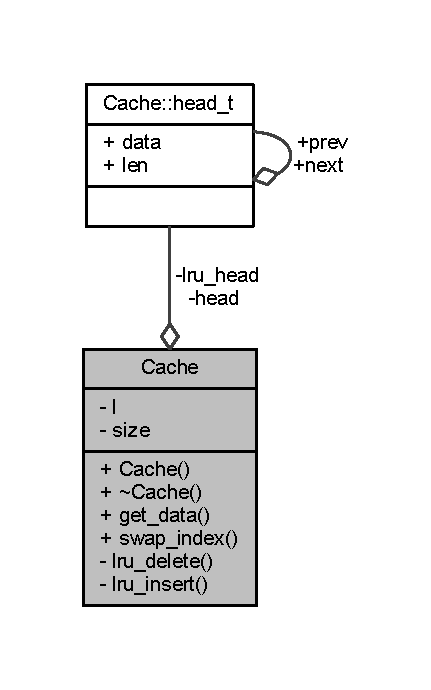
\includegraphics[width=207pt]{class_cache__coll__graph}
\end{center}
\end{figure}
\subsection*{클래스}
\begin{DoxyCompactItemize}
\item 
struct \hyperlink{struct_cache_1_1head__t}{head\+\_\+t}
\end{DoxyCompactItemize}
\subsection*{Public 멤버 함수}
\begin{DoxyCompactItemize}
\item 
\hyperlink{class_cache_a2823f543d4f9b92c29472b904961afe1}{Cache} (int \hyperlink{class_cache_a8f5881aa763cb4af5cfb7b6bda0cff35}{l}, long int \hyperlink{class_cache_af50a89d0734a160cf812384df64599f9}{size})
\item 
\hyperlink{class_cache_af8b171a6c49d88d3ba179477484b9d48}{$\sim$\+Cache} ()
\item 
int \hyperlink{class_cache_aca49263fb34641e208884cc223b25317}{get\+\_\+data} (const int index, \hyperlink{svm_8cpp_a8755d90a54ecfb8d15051af3e0542592}{Qfloat} $\ast$$\ast$data, int len)
\item 
void \hyperlink{class_cache_aaff2dc955f9492c044c98a5f09cfddcc}{swap\+\_\+index} (int i, int j)
\end{DoxyCompactItemize}
\subsection*{Private 멤버 함수}
\begin{DoxyCompactItemize}
\item 
void \hyperlink{class_cache_ab83abc6ded621fa2575e3a44421e0cb4}{lru\+\_\+delete} (\hyperlink{struct_cache_1_1head__t}{head\+\_\+t} $\ast$h)
\item 
void \hyperlink{class_cache_a51e5ffc28e2ec6662ae13ab78ccc2243}{lru\+\_\+insert} (\hyperlink{struct_cache_1_1head__t}{head\+\_\+t} $\ast$h)
\end{DoxyCompactItemize}
\subsection*{Private 속성}
\begin{DoxyCompactItemize}
\item 
int \hyperlink{class_cache_a8f5881aa763cb4af5cfb7b6bda0cff35}{l}
\item 
long int \hyperlink{class_cache_af50a89d0734a160cf812384df64599f9}{size}
\item 
\hyperlink{struct_cache_1_1head__t}{head\+\_\+t} $\ast$ \hyperlink{class_cache_aaf3674e8de1e3896dba64b4caac79f0a}{head}
\item 
\hyperlink{struct_cache_1_1head__t}{head\+\_\+t} \hyperlink{class_cache_a91fc6bd9c69ed37e8e0499da8d47794e}{lru\+\_\+head}
\end{DoxyCompactItemize}


\subsection{상세한 설명}


svm.\+cpp 파일의 67 번째 라인에서 정의되었습니다.



\subsection{생성자 \& 소멸자 문서화}
\hypertarget{class_cache_a2823f543d4f9b92c29472b904961afe1}{\index{Cache@{Cache}!Cache@{Cache}}
\index{Cache@{Cache}!Cache@{Cache}}
\subsubsection[{Cache}]{\setlength{\rightskip}{0pt plus 5cm}Cache\+::\+Cache (
\begin{DoxyParamCaption}
\item[{int}]{l, }
\item[{long int}]{size}
\end{DoxyParamCaption}
)}}\label{class_cache_a2823f543d4f9b92c29472b904961afe1}


svm.\+cpp 파일의 94 번째 라인에서 정의되었습니다.


\begin{DoxyCode}
94                                  :\hyperlink{class_cache_a8f5881aa763cb4af5cfb7b6bda0cff35}{l}(l\_),\hyperlink{class_cache_af50a89d0734a160cf812384df64599f9}{size}(size\_)
95 \{
96     \hyperlink{class_cache_aaf3674e8de1e3896dba64b4caac79f0a}{head} = (head\_t *)calloc(\hyperlink{class_cache_a8f5881aa763cb4af5cfb7b6bda0cff35}{l},\textcolor{keyword}{sizeof}(head\_t)); \textcolor{comment}{// initialized to 0}
97     \hyperlink{class_cache_af50a89d0734a160cf812384df64599f9}{size} /= \textcolor{keyword}{sizeof}(\hyperlink{svm_8cpp_a8755d90a54ecfb8d15051af3e0542592}{Qfloat});
98     \hyperlink{class_cache_af50a89d0734a160cf812384df64599f9}{size} -= \hyperlink{class_cache_a8f5881aa763cb4af5cfb7b6bda0cff35}{l} * \textcolor{keyword}{sizeof}(head\_t) / \textcolor{keyword}{sizeof}(\hyperlink{svm_8cpp_a8755d90a54ecfb8d15051af3e0542592}{Qfloat});
99     \hyperlink{class_cache_af50a89d0734a160cf812384df64599f9}{size} = \hyperlink{svm_8cpp_a7cba98555a7346b01e4cc06205527d8a}{max}(\hyperlink{class_cache_af50a89d0734a160cf812384df64599f9}{size}, 2 * (\textcolor{keywordtype}{long} \textcolor{keywordtype}{int}) \hyperlink{class_cache_a8f5881aa763cb4af5cfb7b6bda0cff35}{l}); \textcolor{comment}{// cache must be large enough for two columns}
100     \hyperlink{class_cache_a91fc6bd9c69ed37e8e0499da8d47794e}{lru\_head}.\hyperlink{struct_cache_1_1head__t_aa152a104ec07250949c234d164f5f3fd}{next} = \hyperlink{class_cache_a91fc6bd9c69ed37e8e0499da8d47794e}{lru\_head}.\hyperlink{struct_cache_1_1head__t_a82b1a4d1a105769f85cce8d51c19860e}{prev} = &\hyperlink{class_cache_a91fc6bd9c69ed37e8e0499da8d47794e}{lru\_head};
101 \}
\end{DoxyCode}


이 함수 내부에서 호출하는 함수들에 대한 그래프입니다.\+:
\nopagebreak
\begin{figure}[H]
\begin{center}
\leavevmode
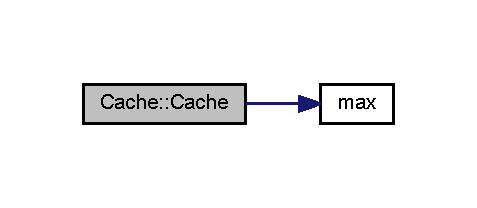
\includegraphics[width=229pt]{class_cache_a2823f543d4f9b92c29472b904961afe1_cgraph}
\end{center}
\end{figure}


\hypertarget{class_cache_af8b171a6c49d88d3ba179477484b9d48}{\index{Cache@{Cache}!````~Cache@{$\sim$\+Cache}}
\index{````~Cache@{$\sim$\+Cache}!Cache@{Cache}}
\subsubsection[{$\sim$\+Cache}]{\setlength{\rightskip}{0pt plus 5cm}Cache\+::$\sim$\+Cache (
\begin{DoxyParamCaption}
{}
\end{DoxyParamCaption}
)}}\label{class_cache_af8b171a6c49d88d3ba179477484b9d48}


svm.\+cpp 파일의 103 번째 라인에서 정의되었습니다.


\begin{DoxyCode}
104 \{
105     \textcolor{keywordflow}{for}(head\_t *h = \hyperlink{class_cache_a91fc6bd9c69ed37e8e0499da8d47794e}{lru\_head}.\hyperlink{struct_cache_1_1head__t_aa152a104ec07250949c234d164f5f3fd}{next}; h != &\hyperlink{class_cache_a91fc6bd9c69ed37e8e0499da8d47794e}{lru\_head}; h=h->\hyperlink{struct_cache_1_1head__t_aa152a104ec07250949c234d164f5f3fd}{next})
106         free(h->data);
107     free(\hyperlink{class_cache_aaf3674e8de1e3896dba64b4caac79f0a}{head});
108 \}
\end{DoxyCode}


\subsection{멤버 함수 문서화}
\hypertarget{class_cache_aca49263fb34641e208884cc223b25317}{\index{Cache@{Cache}!get\+\_\+data@{get\+\_\+data}}
\index{get\+\_\+data@{get\+\_\+data}!Cache@{Cache}}
\subsubsection[{get\+\_\+data}]{\setlength{\rightskip}{0pt plus 5cm}int Cache\+::get\+\_\+data (
\begin{DoxyParamCaption}
\item[{const int}]{index, }
\item[{{\bf Qfloat} $\ast$$\ast$}]{data, }
\item[{int}]{len}
\end{DoxyParamCaption}
)}}\label{class_cache_aca49263fb34641e208884cc223b25317}


svm.\+cpp 파일의 126 번째 라인에서 정의되었습니다.


\begin{DoxyCode}
127 \{
128     head\_t *h = &\hyperlink{class_cache_aaf3674e8de1e3896dba64b4caac79f0a}{head}[index];
129     \textcolor{keywordflow}{if}(h->len) \hyperlink{class_cache_ab83abc6ded621fa2575e3a44421e0cb4}{lru\_delete}(h);
130     \textcolor{keywordtype}{int} more = len - h->len;
131 
132     \textcolor{keywordflow}{if}(more > 0)
133     \{
134         \textcolor{comment}{// free old space}
135         \textcolor{keywordflow}{while}(\hyperlink{class_cache_af50a89d0734a160cf812384df64599f9}{size} < more)
136         \{
137             head\_t *old = \hyperlink{class_cache_a91fc6bd9c69ed37e8e0499da8d47794e}{lru\_head}.\hyperlink{struct_cache_1_1head__t_aa152a104ec07250949c234d164f5f3fd}{next};
138             \hyperlink{class_cache_ab83abc6ded621fa2575e3a44421e0cb4}{lru\_delete}(old);
139             free(old->data);
140             \hyperlink{class_cache_af50a89d0734a160cf812384df64599f9}{size} += old->len;
141             old->data = 0;
142             old->len = 0;
143         \}
144 
145         \textcolor{comment}{// allocate new space}
146         h->data = (\hyperlink{svm_8cpp_a8755d90a54ecfb8d15051af3e0542592}{Qfloat} *)realloc(h->data,\textcolor{keyword}{sizeof}(\hyperlink{svm_8cpp_a8755d90a54ecfb8d15051af3e0542592}{Qfloat})*len);
147         \hyperlink{class_cache_af50a89d0734a160cf812384df64599f9}{size} -= more;
148         \hyperlink{svm_8cpp_a91e77fa16b1c9bbbf90f2eea392997b1}{swap}(h->len,len);
149     \}
150 
151     \hyperlink{class_cache_a51e5ffc28e2ec6662ae13ab78ccc2243}{lru\_insert}(h);
152     *data = h->data;
153     \textcolor{keywordflow}{return} len;
154 \}
\end{DoxyCode}


이 함수 내부에서 호출하는 함수들에 대한 그래프입니다.\+:
\nopagebreak
\begin{figure}[H]
\begin{center}
\leavevmode
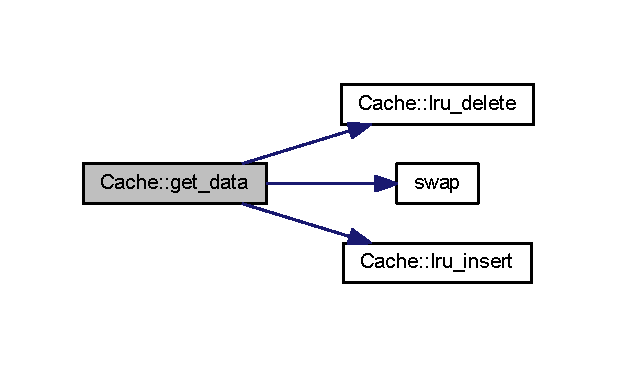
\includegraphics[width=296pt]{class_cache_aca49263fb34641e208884cc223b25317_cgraph}
\end{center}
\end{figure}




이 함수를 호출하는 함수들에 대한 그래프입니다.\+:
\nopagebreak
\begin{figure}[H]
\begin{center}
\leavevmode
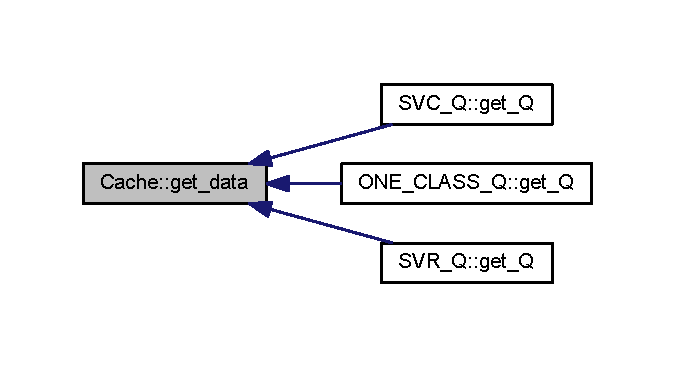
\includegraphics[width=324pt]{class_cache_aca49263fb34641e208884cc223b25317_icgraph}
\end{center}
\end{figure}


\hypertarget{class_cache_ab83abc6ded621fa2575e3a44421e0cb4}{\index{Cache@{Cache}!lru\+\_\+delete@{lru\+\_\+delete}}
\index{lru\+\_\+delete@{lru\+\_\+delete}!Cache@{Cache}}
\subsubsection[{lru\+\_\+delete}]{\setlength{\rightskip}{0pt plus 5cm}void Cache\+::lru\+\_\+delete (
\begin{DoxyParamCaption}
\item[{{\bf head\+\_\+t} $\ast$}]{h}
\end{DoxyParamCaption}
)\hspace{0.3cm}{\ttfamily [private]}}}\label{class_cache_ab83abc6ded621fa2575e3a44421e0cb4}


svm.\+cpp 파일의 110 번째 라인에서 정의되었습니다.


\begin{DoxyCode}
111 \{
112     \textcolor{comment}{// delete from current location}
113     h->prev->next = h->next;
114     h->next->prev = h->prev;
115 \}
\end{DoxyCode}


이 함수를 호출하는 함수들에 대한 그래프입니다.\+:
\nopagebreak
\begin{figure}[H]
\begin{center}
\leavevmode
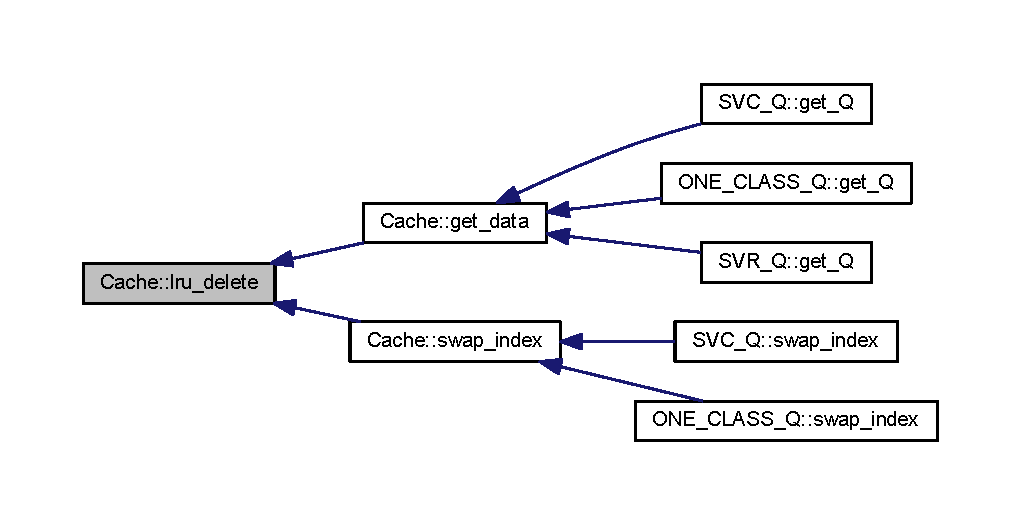
\includegraphics[width=350pt]{class_cache_ab83abc6ded621fa2575e3a44421e0cb4_icgraph}
\end{center}
\end{figure}


\hypertarget{class_cache_a51e5ffc28e2ec6662ae13ab78ccc2243}{\index{Cache@{Cache}!lru\+\_\+insert@{lru\+\_\+insert}}
\index{lru\+\_\+insert@{lru\+\_\+insert}!Cache@{Cache}}
\subsubsection[{lru\+\_\+insert}]{\setlength{\rightskip}{0pt plus 5cm}void Cache\+::lru\+\_\+insert (
\begin{DoxyParamCaption}
\item[{{\bf head\+\_\+t} $\ast$}]{h}
\end{DoxyParamCaption}
)\hspace{0.3cm}{\ttfamily [private]}}}\label{class_cache_a51e5ffc28e2ec6662ae13ab78ccc2243}


svm.\+cpp 파일의 117 번째 라인에서 정의되었습니다.


\begin{DoxyCode}
118 \{
119     \textcolor{comment}{// insert to last position}
120     h->next = &\hyperlink{class_cache_a91fc6bd9c69ed37e8e0499da8d47794e}{lru\_head};
121     h->\hyperlink{struct_cache_1_1head__t_a82b1a4d1a105769f85cce8d51c19860e}{prev} = \hyperlink{class_cache_a91fc6bd9c69ed37e8e0499da8d47794e}{lru\_head}.\hyperlink{struct_cache_1_1head__t_a82b1a4d1a105769f85cce8d51c19860e}{prev};
122     h->\hyperlink{struct_cache_1_1head__t_a82b1a4d1a105769f85cce8d51c19860e}{prev}->\hyperlink{struct_cache_1_1head__t_aa152a104ec07250949c234d164f5f3fd}{next} = h;
123     h->\hyperlink{struct_cache_1_1head__t_aa152a104ec07250949c234d164f5f3fd}{next}->\hyperlink{struct_cache_1_1head__t_a82b1a4d1a105769f85cce8d51c19860e}{prev} = h;
124 \}
\end{DoxyCode}


이 함수를 호출하는 함수들에 대한 그래프입니다.\+:
\nopagebreak
\begin{figure}[H]
\begin{center}
\leavevmode
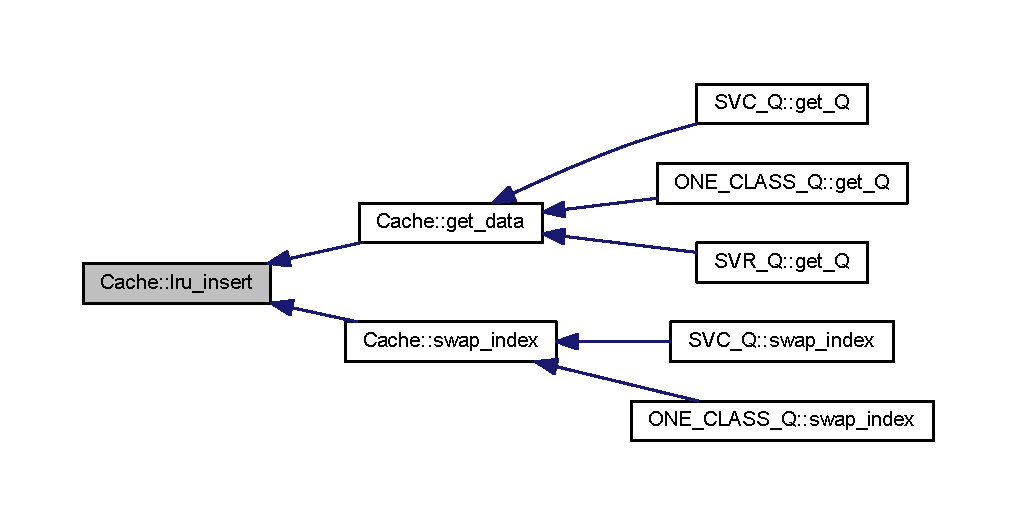
\includegraphics[width=350pt]{class_cache_a51e5ffc28e2ec6662ae13ab78ccc2243_icgraph}
\end{center}
\end{figure}


\hypertarget{class_cache_aaff2dc955f9492c044c98a5f09cfddcc}{\index{Cache@{Cache}!swap\+\_\+index@{swap\+\_\+index}}
\index{swap\+\_\+index@{swap\+\_\+index}!Cache@{Cache}}
\subsubsection[{swap\+\_\+index}]{\setlength{\rightskip}{0pt plus 5cm}void Cache\+::swap\+\_\+index (
\begin{DoxyParamCaption}
\item[{int}]{i, }
\item[{int}]{j}
\end{DoxyParamCaption}
)}}\label{class_cache_aaff2dc955f9492c044c98a5f09cfddcc}


svm.\+cpp 파일의 156 번째 라인에서 정의되었습니다.


\begin{DoxyCode}
157 \{
158     \textcolor{keywordflow}{if}(i==j) \textcolor{keywordflow}{return};
159 
160     \textcolor{keywordflow}{if}(\hyperlink{class_cache_aaf3674e8de1e3896dba64b4caac79f0a}{head}[i].len) \hyperlink{class_cache_ab83abc6ded621fa2575e3a44421e0cb4}{lru\_delete}(&\hyperlink{class_cache_aaf3674e8de1e3896dba64b4caac79f0a}{head}[i]);
161     \textcolor{keywordflow}{if}(\hyperlink{class_cache_aaf3674e8de1e3896dba64b4caac79f0a}{head}[j].len) \hyperlink{class_cache_ab83abc6ded621fa2575e3a44421e0cb4}{lru\_delete}(&\hyperlink{class_cache_aaf3674e8de1e3896dba64b4caac79f0a}{head}[j]);
162     \hyperlink{svm_8cpp_a91e77fa16b1c9bbbf90f2eea392997b1}{swap}(\hyperlink{class_cache_aaf3674e8de1e3896dba64b4caac79f0a}{head}[i].data,\hyperlink{class_cache_aaf3674e8de1e3896dba64b4caac79f0a}{head}[j].data);
163     \hyperlink{svm_8cpp_a91e77fa16b1c9bbbf90f2eea392997b1}{swap}(\hyperlink{class_cache_aaf3674e8de1e3896dba64b4caac79f0a}{head}[i].len,\hyperlink{class_cache_aaf3674e8de1e3896dba64b4caac79f0a}{head}[j].len);
164     \textcolor{keywordflow}{if}(\hyperlink{class_cache_aaf3674e8de1e3896dba64b4caac79f0a}{head}[i].len) \hyperlink{class_cache_a51e5ffc28e2ec6662ae13ab78ccc2243}{lru\_insert}(&\hyperlink{class_cache_aaf3674e8de1e3896dba64b4caac79f0a}{head}[i]);
165     \textcolor{keywordflow}{if}(\hyperlink{class_cache_aaf3674e8de1e3896dba64b4caac79f0a}{head}[j].len) \hyperlink{class_cache_a51e5ffc28e2ec6662ae13ab78ccc2243}{lru\_insert}(&\hyperlink{class_cache_aaf3674e8de1e3896dba64b4caac79f0a}{head}[j]);
166 
167     \textcolor{keywordflow}{if}(i>j) \hyperlink{svm_8cpp_a91e77fa16b1c9bbbf90f2eea392997b1}{swap}(i,j);
168     \textcolor{keywordflow}{for}(head\_t *h = \hyperlink{class_cache_a91fc6bd9c69ed37e8e0499da8d47794e}{lru\_head}.\hyperlink{struct_cache_1_1head__t_aa152a104ec07250949c234d164f5f3fd}{next}; h!=&\hyperlink{class_cache_a91fc6bd9c69ed37e8e0499da8d47794e}{lru\_head}; h=h->\hyperlink{struct_cache_1_1head__t_aa152a104ec07250949c234d164f5f3fd}{next})
169     \{
170         \textcolor{keywordflow}{if}(h->len > i)
171         \{
172             \textcolor{keywordflow}{if}(h->len > j)
173                 \hyperlink{svm_8cpp_a91e77fa16b1c9bbbf90f2eea392997b1}{swap}(h->data[i],h->data[j]);
174             \textcolor{keywordflow}{else}
175             \{
176                 \textcolor{comment}{// give up}
177                 \hyperlink{class_cache_ab83abc6ded621fa2575e3a44421e0cb4}{lru\_delete}(h);
178                 free(h->data);
179                 \hyperlink{class_cache_af50a89d0734a160cf812384df64599f9}{size} += h->len;
180                 h->data = 0;
181                 h->len = 0;
182             \}
183         \}
184     \}
185 \}
\end{DoxyCode}


이 함수 내부에서 호출하는 함수들에 대한 그래프입니다.\+:
\nopagebreak
\begin{figure}[H]
\begin{center}
\leavevmode
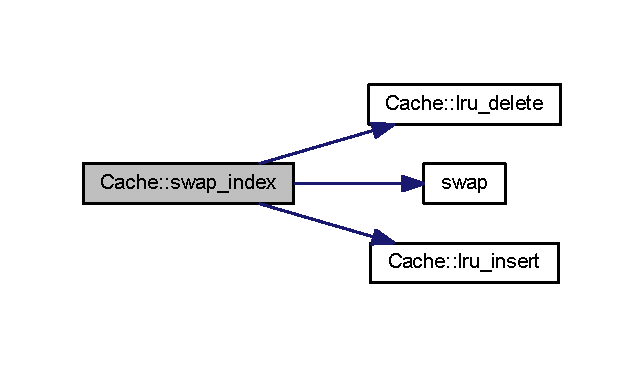
\includegraphics[width=309pt]{class_cache_aaff2dc955f9492c044c98a5f09cfddcc_cgraph}
\end{center}
\end{figure}




이 함수를 호출하는 함수들에 대한 그래프입니다.\+:
\nopagebreak
\begin{figure}[H]
\begin{center}
\leavevmode
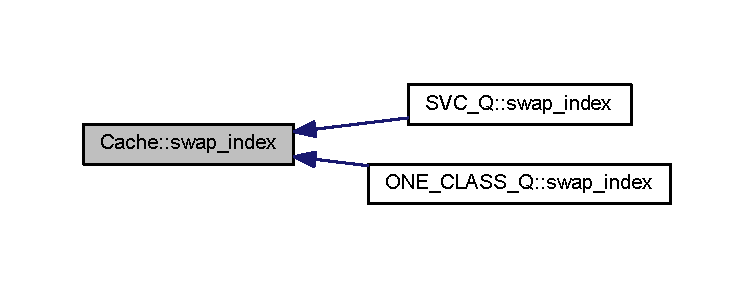
\includegraphics[width=350pt]{class_cache_aaff2dc955f9492c044c98a5f09cfddcc_icgraph}
\end{center}
\end{figure}




\subsection{멤버 데이타 문서화}
\hypertarget{class_cache_aaf3674e8de1e3896dba64b4caac79f0a}{\index{Cache@{Cache}!head@{head}}
\index{head@{head}!Cache@{Cache}}
\subsubsection[{head}]{\setlength{\rightskip}{0pt plus 5cm}{\bf head\+\_\+t}$\ast$ Cache\+::head\hspace{0.3cm}{\ttfamily [private]}}}\label{class_cache_aaf3674e8de1e3896dba64b4caac79f0a}


svm.\+cpp 파일의 88 번째 라인에서 정의되었습니다.

\hypertarget{class_cache_a8f5881aa763cb4af5cfb7b6bda0cff35}{\index{Cache@{Cache}!l@{l}}
\index{l@{l}!Cache@{Cache}}
\subsubsection[{l}]{\setlength{\rightskip}{0pt plus 5cm}int Cache\+::l\hspace{0.3cm}{\ttfamily [private]}}}\label{class_cache_a8f5881aa763cb4af5cfb7b6bda0cff35}


svm.\+cpp 파일의 79 번째 라인에서 정의되었습니다.

\hypertarget{class_cache_a91fc6bd9c69ed37e8e0499da8d47794e}{\index{Cache@{Cache}!lru\+\_\+head@{lru\+\_\+head}}
\index{lru\+\_\+head@{lru\+\_\+head}!Cache@{Cache}}
\subsubsection[{lru\+\_\+head}]{\setlength{\rightskip}{0pt plus 5cm}{\bf head\+\_\+t} Cache\+::lru\+\_\+head\hspace{0.3cm}{\ttfamily [private]}}}\label{class_cache_a91fc6bd9c69ed37e8e0499da8d47794e}


svm.\+cpp 파일의 89 번째 라인에서 정의되었습니다.

\hypertarget{class_cache_af50a89d0734a160cf812384df64599f9}{\index{Cache@{Cache}!size@{size}}
\index{size@{size}!Cache@{Cache}}
\subsubsection[{size}]{\setlength{\rightskip}{0pt plus 5cm}long int Cache\+::size\hspace{0.3cm}{\ttfamily [private]}}}\label{class_cache_af50a89d0734a160cf812384df64599f9}


svm.\+cpp 파일의 80 번째 라인에서 정의되었습니다.



이 클래스에 대한 문서화 페이지는 다음의 파일로부터 생성되었습니다.\+:\begin{DoxyCompactItemize}
\item 
src/\+Calculator/\hyperlink{svm_8cpp}{svm.\+cpp}\end{DoxyCompactItemize}

\hypertarget{class_calculate}{\section{Calculate 클래스 참조}
\label{class_calculate}\index{Calculate@{Calculate}}
}


입력받은 수식을 계산해 주는 Class  




{\ttfamily \#include $<$Calculate.\+h$>$}



Calculate에 대한 협력 다이어그램\+:
\nopagebreak
\begin{figure}[H]
\begin{center}
\leavevmode
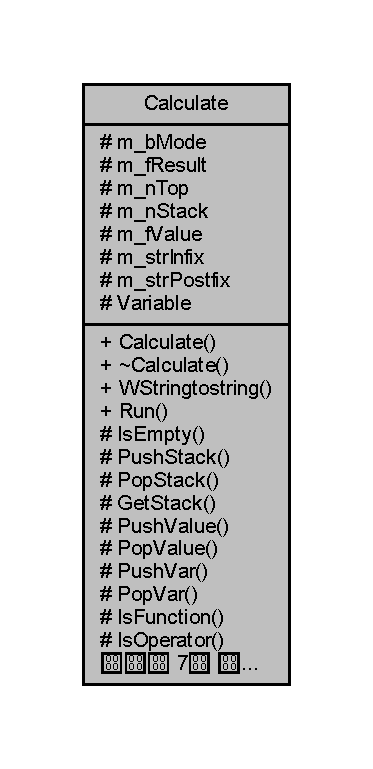
\includegraphics[width=179pt]{class_calculate__coll__graph}
\end{center}
\end{figure}
\subsection*{Public 멤버 함수}
\begin{DoxyCompactItemize}
\item 
\hyperlink{class_calculate_a9324cfcffaf7004813243ab39b003c66}{Calculate} ()
\item 
\hyperlink{class_calculate_aeb9c1ffe2bcc1bb58c1c2c591c0e8827}{$\sim$\+Calculate} ()
\item 
std\+::string \hyperlink{class_calculate_a50d0dfb999edd48ae45b8023e6a69d6a}{W\+Stringtostring} (Tizen\+::\+Base\+::\+String input)
\item 
double $\ast$ \hyperlink{class_calculate_a0ad76f7ee31bea1dec46e560d10fca75}{Run} (String string)
\end{DoxyCompactItemize}
\subsection*{Protected 멤버 함수}
\begin{DoxyCompactItemize}
\item 
\hyperlink{_calculate_8h_a3e5b8192e7d9ffaf3542f1210aec18dd}{B\+O\+O\+L} \hyperlink{class_calculate_a689df9c34a1e9f4bb55a8487a9761380}{Is\+Empty} ()
\item 
int \hyperlink{class_calculate_a4981fb0c9805e7cc7418c4c8089be189}{Push\+Stack} (int)
\item 
int \hyperlink{class_calculate_a2ca7f9e37fc39bc7230fac0bdda0fc87}{Pop\+Stack} ()
\item 
int \hyperlink{class_calculate_a51b9a5aa2196ff202ebd8c7414f1f830}{Get\+Stack} ()
\item 
double \hyperlink{class_calculate_a25e1df1079c2b915fc3c755406f44948}{Push\+Value} (double)
\item 
double \hyperlink{class_calculate_a1a970f9eaf0ce1296acf354fb1eee7f6}{Pop\+Value} ()
\item 
void \hyperlink{class_calculate_a0031446d6885f82dd36f45665d5c5ac1}{Push\+Var} (char, double)
\item 
double \hyperlink{class_calculate_a0e154ef32a3b779b31af1a2724c92b95}{Pop\+Var} (char)
\item 
int \hyperlink{class_calculate_a753ebfbfca50f0421eae09729794fbf1}{Is\+Function} (const char $\ast$)
\item 
int \hyperlink{class_calculate_a32f5599bfe127c4e90d356ff883c624b}{Is\+Operator} (int)
\item 
int \hyperlink{class_calculate_ab76e8ed2e961699a73807f9af6b72aa9}{Get\+Order} (int)
\item 
bool \hyperlink{class_calculate_a2a0f619344c8154e8740819942ccdddd}{Result\+Range\+Check} (double, double, char)
\item 
bool \hyperlink{class_calculate_ab9429972ea44b6d1e57f9bdf7f377e34}{Result\+Range\+Check} (double)
\item 
void \hyperlink{class_calculate_aa8f0261822a44685b37dfe22a6eacc04}{Init} ()
\item 
\hyperlink{_calculate_8h_a3e5b8192e7d9ffaf3542f1210aec18dd}{B\+O\+O\+L} \hyperlink{class_calculate_a680527f598a4b37febfcdeb21dea6e9c}{Read} (std\+::string string)
\item 
void \hyperlink{class_calculate_a81090066a9bc2e77432198e45850eb5d}{Postfix} ()
\item 
void \hyperlink{class_calculate_af81d8f0097a86c858825c3deef573697}{Evaluate} ()
\end{DoxyCompactItemize}
\subsection*{Protected 속성}
\begin{DoxyCompactItemize}
\item 
\hyperlink{_calculate_8h_a3e5b8192e7d9ffaf3542f1210aec18dd}{B\+O\+O\+L} \hyperlink{class_calculate_a91ed53268a8f29f54757037bc28d35e0}{m\+\_\+b\+Mode}
\item 
double $\ast$ \hyperlink{class_calculate_a5ffe97b9c4358acf90360d328b9144c0}{m\+\_\+f\+Result}
\item 
int \hyperlink{class_calculate_a9f6afe7d8278100e1f27977aaeba0a72}{m\+\_\+n\+Top}
\item 
int $\ast$ \hyperlink{class_calculate_ae2a302680f654bfa735b1dc4f34814b6}{m\+\_\+n\+Stack}
\item 
double $\ast$ \hyperlink{class_calculate_a7ded18ea2282684cf9570cceadbcbf37}{m\+\_\+f\+Value}
\item 
char $\ast$ \hyperlink{class_calculate_a1b964b49f9a186fa02643c1361ccd4ab}{m\+\_\+str\+Infix}
\item 
char $\ast$ \hyperlink{class_calculate_aceafe6d40cd154f9535dc971c1e9bb7a}{m\+\_\+str\+Postfix}
\end{DoxyCompactItemize}
\subsection*{정적 Protected 속성}
\begin{DoxyCompactItemize}
\item 
static double \hyperlink{class_calculate_a75fc03f230ef600e36be8073acc34216}{Variable} \mbox{[}26\mbox{]}
\end{DoxyCompactItemize}


\subsection{상세한 설명}
입력받은 수식을 계산해 주는 Class 

String 형식으로 입력받은 계산식을 infix에서 postfix로 바꾸어 계산 순서에 맞게 계산해주고 그 계산값을 double형으로 return해준다. \begin{DoxyDate}{날짜}
2014-\/12-\/13 
\end{DoxyDate}
\begin{DoxyVersion}{버전}
0.\+0.\+1 
\end{DoxyVersion}


Calculate.\+h 파일의 28 번째 라인에서 정의되었습니다.



\subsection{생성자 \& 소멸자 문서화}
\hypertarget{class_calculate_a9324cfcffaf7004813243ab39b003c66}{\index{Calculate@{Calculate}!Calculate@{Calculate}}
\index{Calculate@{Calculate}!Calculate@{Calculate}}
\subsubsection[{Calculate}]{\setlength{\rightskip}{0pt plus 5cm}Calculate\+::\+Calculate (
\begin{DoxyParamCaption}
{}
\end{DoxyParamCaption}
)}}\label{class_calculate_a9324cfcffaf7004813243ab39b003c66}


Calculate.\+cpp 파일의 55 번째 라인에서 정의되었습니다.


\begin{DoxyCode}
55                      \{
56     \hyperlink{class_calculate_aa8f0261822a44685b37dfe22a6eacc04}{Init}();
57 \}
\end{DoxyCode}
\hypertarget{class_calculate_aeb9c1ffe2bcc1bb58c1c2c591c0e8827}{\index{Calculate@{Calculate}!````~Calculate@{$\sim$\+Calculate}}
\index{````~Calculate@{$\sim$\+Calculate}!Calculate@{Calculate}}
\subsubsection[{$\sim$\+Calculate}]{\setlength{\rightskip}{0pt plus 5cm}Calculate\+::$\sim$\+Calculate (
\begin{DoxyParamCaption}
{}
\end{DoxyParamCaption}
)}}\label{class_calculate_aeb9c1ffe2bcc1bb58c1c2c591c0e8827}


Calculate.\+cpp 파일의 59 번째 라인에서 정의되었습니다.


\begin{DoxyCode}
59                       \{
60     \hyperlink{class_calculate_a5ffe97b9c4358acf90360d328b9144c0}{m\_fResult} = \textcolor{keyword}{new} \textcolor{keywordtype}{double}[2];
61     \hyperlink{class_calculate_a5ffe97b9c4358acf90360d328b9144c0}{m\_fResult}[1] = \hyperlink{_calculate_8cpp_a043810f41cc510e36a892f3b65fac5cb}{RESULT\_OK};
62     \hyperlink{class_calculate_a91ed53268a8f29f54757037bc28d35e0}{m\_bMode} = \hyperlink{_calculate_8h_a3e5b8192e7d9ffaf3542f1210aec18ddaa1e095cc966dbecf6a0d8aad75348d1a}{FALSE};
63     \hyperlink{class_calculate_a9f6afe7d8278100e1f27977aaeba0a72}{m\_nTop} = 0;
64     \textcolor{keywordflow}{if} (\hyperlink{class_calculate_ae2a302680f654bfa735b1dc4f34814b6}{m\_nStack})
65         \textcolor{keyword}{delete}[] \hyperlink{class_calculate_ae2a302680f654bfa735b1dc4f34814b6}{m\_nStack};
66     \textcolor{keywordflow}{if} (\hyperlink{class_calculate_a7ded18ea2282684cf9570cceadbcbf37}{m\_fValue})
67         \textcolor{keyword}{delete}[] \hyperlink{class_calculate_a7ded18ea2282684cf9570cceadbcbf37}{m\_fValue};
68     \textcolor{keywordflow}{if} (\hyperlink{class_calculate_a1b964b49f9a186fa02643c1361ccd4ab}{m\_strInfix})
69         \textcolor{keyword}{delete}[] \hyperlink{class_calculate_a1b964b49f9a186fa02643c1361ccd4ab}{m\_strInfix};
70     \textcolor{keywordflow}{if} (\hyperlink{class_calculate_aceafe6d40cd154f9535dc971c1e9bb7a}{m\_strPostfix})
71         \textcolor{keyword}{delete}[] \hyperlink{class_calculate_aceafe6d40cd154f9535dc971c1e9bb7a}{m\_strPostfix};
72 \}
\end{DoxyCode}


\subsection{멤버 함수 문서화}
\hypertarget{class_calculate_af81d8f0097a86c858825c3deef573697}{\index{Calculate@{Calculate}!Evaluate@{Evaluate}}
\index{Evaluate@{Evaluate}!Calculate@{Calculate}}
\subsubsection[{Evaluate}]{\setlength{\rightskip}{0pt plus 5cm}void Calculate\+::\+Evaluate (
\begin{DoxyParamCaption}
{}
\end{DoxyParamCaption}
)\hspace{0.3cm}{\ttfamily [protected]}}}\label{class_calculate_af81d8f0097a86c858825c3deef573697}


Calculate.\+cpp 파일의 322 번째 라인에서 정의되었습니다.


\begin{DoxyCode}
322                          \{
323     \hyperlink{class_calculate_a9f6afe7d8278100e1f27977aaeba0a72}{m\_nTop} = 0;
324     \hyperlink{class_calculate_a7ded18ea2282684cf9570cceadbcbf37}{m\_fValue} = \textcolor{keyword}{new} \textcolor{keywordtype}{double}[\hyperlink{_calculate_8cpp_a392fb874e547e582e9c66a08a1f23326}{MAX}];
325     \textcolor{keywordtype}{int} i = 0;
326     \textcolor{keywordtype}{char} variable;
327 
328     \textcolor{keywordflow}{while} (\hyperlink{class_calculate_aceafe6d40cd154f9535dc971c1e9bb7a}{m\_strPostfix}[i]) \{
329         \textcolor{comment}{// 숫자 처리 부분}
330         \textcolor{keywordflow}{if} (isdigit(\hyperlink{class_calculate_aceafe6d40cd154f9535dc971c1e9bb7a}{m\_strPostfix}[i]) || \hyperlink{class_calculate_aceafe6d40cd154f9535dc971c1e9bb7a}{m\_strPostfix}[i] == \textcolor{charliteral}{'.'}) \{
331             \textcolor{keywordtype}{char} *number = \textcolor{keyword}{new} \textcolor{keywordtype}{char}[\hyperlink{_calculate_8cpp_a5c3a83864bf5991d09aa5c2abb911bf0}{TOKEN}];
332             \textcolor{keywordtype}{int} j = 0;
333             \textcolor{keywordflow}{while} (isdigit(\hyperlink{class_calculate_aceafe6d40cd154f9535dc971c1e9bb7a}{m\_strPostfix}[i]) || \hyperlink{class_calculate_aceafe6d40cd154f9535dc971c1e9bb7a}{m\_strPostfix}[i] == \textcolor{charliteral}{'.'})
334                 number[j++] = \hyperlink{class_calculate_aceafe6d40cd154f9535dc971c1e9bb7a}{m\_strPostfix}[i++];
335             number[j] = NULL;
336             \hyperlink{class_calculate_a25e1df1079c2b915fc3c755406f44948}{PushValue}(atof(number));
337         \}
338         \textcolor{comment}{// 연산자 처리 부분}
339         \textcolor{keywordflow}{else} \textcolor{keywordflow}{if} (\hyperlink{class_calculate_aceafe6d40cd154f9535dc971c1e9bb7a}{m\_strPostfix}[i] == \textcolor{charliteral}{'~'}) \textcolor{comment}{// 부호연산자}
340                 \{
341             \textcolor{keywordtype}{double} rvar = \hyperlink{class_calculate_a1a970f9eaf0ce1296acf354fb1eee7f6}{PopValue}();
342             \hyperlink{class_calculate_a25e1df1079c2b915fc3c755406f44948}{PushValue}(-1 * rvar);
343             i++;
344         \} \textcolor{keywordflow}{else} \textcolor{keywordflow}{if} (\hyperlink{class_calculate_aceafe6d40cd154f9535dc971c1e9bb7a}{m\_strPostfix}[i] == \textcolor{charliteral}{'+'}) \{
345             \textcolor{keywordtype}{double} rvar = \hyperlink{class_calculate_a1a970f9eaf0ce1296acf354fb1eee7f6}{PopValue}();
346             \textcolor{keywordtype}{double} lvar = \hyperlink{class_calculate_a1a970f9eaf0ce1296acf354fb1eee7f6}{PopValue}();
347             \textcolor{keywordflow}{if} (\hyperlink{class_calculate_a2a0f619344c8154e8740819942ccdddd}{ResultRangeCheck}(lvar, rvar, \textcolor{charliteral}{'+'}))
348                 \hyperlink{class_calculate_a25e1df1079c2b915fc3c755406f44948}{PushValue}(lvar + rvar);
349             \textcolor{keywordflow}{else} \{
350                 \hyperlink{class_calculate_a5ffe97b9c4358acf90360d328b9144c0}{m\_fResult}[1] = \hyperlink{_calculate_8cpp_a113621396df65ce36c6b41262ff2f884}{RESULT\_OVERFLOW};
351                 \hyperlink{class_calculate_a5ffe97b9c4358acf90360d328b9144c0}{m\_fResult}[0] = 0;
352                 \textcolor{keywordflow}{return};
353             \}
354             \textcolor{comment}{//PushValue(lvar + rvar);}
355             i++;
356         \} \textcolor{keywordflow}{else} \textcolor{keywordflow}{if} (\hyperlink{class_calculate_aceafe6d40cd154f9535dc971c1e9bb7a}{m\_strPostfix}[i] == \textcolor{charliteral}{'-'}) \{
357             \textcolor{keywordtype}{double} rvar = \hyperlink{class_calculate_a1a970f9eaf0ce1296acf354fb1eee7f6}{PopValue}();
358             \textcolor{keywordtype}{double} lvar = \hyperlink{class_calculate_a1a970f9eaf0ce1296acf354fb1eee7f6}{PopValue}();
359             \textcolor{keywordflow}{if} (\hyperlink{class_calculate_a2a0f619344c8154e8740819942ccdddd}{ResultRangeCheck}(lvar, rvar, \textcolor{charliteral}{'-'}))
360                 \hyperlink{class_calculate_a25e1df1079c2b915fc3c755406f44948}{PushValue}(lvar - rvar);
361             \textcolor{keywordflow}{else} \{
362                 \hyperlink{class_calculate_a5ffe97b9c4358acf90360d328b9144c0}{m\_fResult}[1] = \hyperlink{_calculate_8cpp_a113621396df65ce36c6b41262ff2f884}{RESULT\_OVERFLOW};
363                 \hyperlink{class_calculate_a5ffe97b9c4358acf90360d328b9144c0}{m\_fResult}[0] = 0;
364                 \textcolor{keywordflow}{return};
365             \}
366             \textcolor{comment}{//PushValue(lvar - rvar);}
367             i++;
368         \} \textcolor{keywordflow}{else} \textcolor{keywordflow}{if} (\hyperlink{class_calculate_aceafe6d40cd154f9535dc971c1e9bb7a}{m\_strPostfix}[i] == \textcolor{charliteral}{'*'}) \{
369             \textcolor{keywordtype}{double} rvar = \hyperlink{class_calculate_a1a970f9eaf0ce1296acf354fb1eee7f6}{PopValue}();
370             \textcolor{keywordtype}{double} lvar = \hyperlink{class_calculate_a1a970f9eaf0ce1296acf354fb1eee7f6}{PopValue}();
371             \textcolor{keywordflow}{if} (\hyperlink{class_calculate_a2a0f619344c8154e8740819942ccdddd}{ResultRangeCheck}(lvar, rvar, \textcolor{charliteral}{'*'}))
372                 \hyperlink{class_calculate_a25e1df1079c2b915fc3c755406f44948}{PushValue}(lvar * rvar);
373             \textcolor{keywordflow}{else} \{
374                 \hyperlink{class_calculate_a5ffe97b9c4358acf90360d328b9144c0}{m\_fResult}[1] = \hyperlink{_calculate_8cpp_a113621396df65ce36c6b41262ff2f884}{RESULT\_OVERFLOW};
375                 \hyperlink{class_calculate_a5ffe97b9c4358acf90360d328b9144c0}{m\_fResult}[0] = 0;
376                 \textcolor{keywordflow}{return};
377             \}
378             \textcolor{comment}{//PushValue(lvar * rvar);}
379             i++;
380         \} \textcolor{keywordflow}{else} \textcolor{keywordflow}{if} (\hyperlink{class_calculate_aceafe6d40cd154f9535dc971c1e9bb7a}{m\_strPostfix}[i] == \textcolor{charliteral}{'/'}) \{
381             \textcolor{keywordtype}{double} rvar = \hyperlink{class_calculate_a1a970f9eaf0ce1296acf354fb1eee7f6}{PopValue}();
382             \textcolor{keywordtype}{double} lvar = \hyperlink{class_calculate_a1a970f9eaf0ce1296acf354fb1eee7f6}{PopValue}();
383             \hyperlink{class_calculate_a25e1df1079c2b915fc3c755406f44948}{PushValue}(lvar / rvar);
384             i++;
385         \} \textcolor{keywordflow}{else} \textcolor{keywordflow}{if} (\hyperlink{class_calculate_aceafe6d40cd154f9535dc971c1e9bb7a}{m\_strPostfix}[i] == \textcolor{charliteral}{'%'}) \{
386             \textcolor{keywordtype}{double} rvar = \hyperlink{class_calculate_a1a970f9eaf0ce1296acf354fb1eee7f6}{PopValue}();
387             \textcolor{keywordtype}{double} lvar = \hyperlink{class_calculate_a1a970f9eaf0ce1296acf354fb1eee7f6}{PopValue}();
388             \hyperlink{class_calculate_a25e1df1079c2b915fc3c755406f44948}{PushValue}(fmod(lvar, rvar));
389             i++;
390         \} \textcolor{keywordflow}{else} \textcolor{keywordflow}{if} (\hyperlink{class_calculate_aceafe6d40cd154f9535dc971c1e9bb7a}{m\_strPostfix}[i] == \textcolor{charliteral}{'^'}) \{
391             \textcolor{keywordtype}{double} rvar = \hyperlink{class_calculate_a1a970f9eaf0ce1296acf354fb1eee7f6}{PopValue}();
392             \textcolor{keywordtype}{double} lvar = \hyperlink{class_calculate_a1a970f9eaf0ce1296acf354fb1eee7f6}{PopValue}();
393             \textcolor{keywordflow}{if} (\hyperlink{class_calculate_a2a0f619344c8154e8740819942ccdddd}{ResultRangeCheck}(lvar, rvar, \textcolor{charliteral}{'^'}))
394                 \hyperlink{class_calculate_a25e1df1079c2b915fc3c755406f44948}{PushValue}(pow(lvar, rvar));
395             \textcolor{keywordflow}{else} \{
396                 \hyperlink{class_calculate_a5ffe97b9c4358acf90360d328b9144c0}{m\_fResult}[1] = \hyperlink{_calculate_8cpp_a113621396df65ce36c6b41262ff2f884}{RESULT\_OVERFLOW};
397                 \hyperlink{class_calculate_a5ffe97b9c4358acf90360d328b9144c0}{m\_fResult}[0] = 0;
398                 \textcolor{keywordflow}{return};
399             \}
400             i++;
401         \}
402         \textcolor{comment}{// factorial}
403         \textcolor{keywordflow}{else} \textcolor{keywordflow}{if} (\hyperlink{class_calculate_aceafe6d40cd154f9535dc971c1e9bb7a}{m\_strPostfix}[i] == \textcolor{charliteral}{'!'}) \{
404             \textcolor{keywordtype}{double} rvar = (int) \hyperlink{class_calculate_a1a970f9eaf0ce1296acf354fb1eee7f6}{PopValue}();
405             \textcolor{keywordtype}{double} result = 1;
406             \textcolor{keywordflow}{for} (; rvar > 0; rvar--) \{
407                 result *= rvar;
408                 \textcolor{keywordflow}{if} (!\hyperlink{class_calculate_a2a0f619344c8154e8740819942ccdddd}{ResultRangeCheck}(result)) \{
409                     \hyperlink{class_calculate_a5ffe97b9c4358acf90360d328b9144c0}{m\_fResult}[1] = \hyperlink{_calculate_8cpp_a113621396df65ce36c6b41262ff2f884}{RESULT\_OVERFLOW};
410                     \hyperlink{class_calculate_a5ffe97b9c4358acf90360d328b9144c0}{m\_fResult}[0] = 0;
411                     \textcolor{keywordflow}{return};
412                 \}
413             \}
414             \hyperlink{class_calculate_a25e1df1079c2b915fc3c755406f44948}{PushValue}(result);
415             i++;
416         \}
417         \textcolor{comment}{//Pi}
418         \textcolor{keywordflow}{else} \textcolor{keywordflow}{if} (\hyperlink{class_calculate_aceafe6d40cd154f9535dc971c1e9bb7a}{m\_strPostfix}[i] == \textcolor{charliteral}{'p'}) \{
419             \hyperlink{class_calculate_a25e1df1079c2b915fc3c755406f44948}{PushValue}(\hyperlink{_calculate_8cpp_ae71449b1cc6e6250b91f539153a7a0d3}{M\_PI});
420             i++;
421         \}
422         \textcolor{comment}{//e}
423         \textcolor{keywordflow}{else} \textcolor{keywordflow}{if} (\hyperlink{class_calculate_aceafe6d40cd154f9535dc971c1e9bb7a}{m\_strPostfix}[i] == \textcolor{charliteral}{'e'}) \{
424             \hyperlink{class_calculate_a25e1df1079c2b915fc3c755406f44948}{PushValue}(\hyperlink{_calculate_8cpp_a9bf5d952c5c93c70f9e66c9794d406c9}{M\_E});
425             i++;
426         \}
427         \textcolor{comment}{//absolute}
428         \textcolor{keywordflow}{else} \textcolor{keywordflow}{if} (\hyperlink{class_calculate_aceafe6d40cd154f9535dc971c1e9bb7a}{m\_strPostfix}[i] == \textcolor{charliteral}{'a'}) \{
429             \textcolor{keywordtype}{double} rvar = \hyperlink{class_calculate_a1a970f9eaf0ce1296acf354fb1eee7f6}{PopValue}();
430             \hyperlink{class_calculate_a25e1df1079c2b915fc3c755406f44948}{PushValue}(fabs(rvar));
431             i++;
432         \}
433         \textcolor{comment}{//sqrt}
434         \textcolor{keywordflow}{else} \textcolor{keywordflow}{if} (\hyperlink{class_calculate_aceafe6d40cd154f9535dc971c1e9bb7a}{m\_strPostfix}[i] == \textcolor{charliteral}{'r'}) \{
435             \textcolor{keywordtype}{double} rvar = \hyperlink{class_calculate_a1a970f9eaf0ce1296acf354fb1eee7f6}{PopValue}();
436             \hyperlink{class_calculate_a25e1df1079c2b915fc3c755406f44948}{PushValue}(sqrt(rvar));
437             i++;
438         \}
439         \textcolor{comment}{//power}
440         \textcolor{keywordflow}{else} \textcolor{keywordflow}{if} (\hyperlink{class_calculate_aceafe6d40cd154f9535dc971c1e9bb7a}{m\_strPostfix}[i] == \textcolor{charliteral}{'^'}) \{
441             \textcolor{keywordtype}{double} rvar = \hyperlink{class_calculate_a1a970f9eaf0ce1296acf354fb1eee7f6}{PopValue}();
442             \textcolor{keywordtype}{double} lvar = \hyperlink{class_calculate_a1a970f9eaf0ce1296acf354fb1eee7f6}{PopValue}();
443             \hyperlink{class_calculate_a25e1df1079c2b915fc3c755406f44948}{PushValue}(pow(lvar, rvar));
444             i++;
445         \}
446         \textcolor{comment}{//exp}
447         \textcolor{keywordflow}{else} \textcolor{keywordflow}{if} (\hyperlink{class_calculate_aceafe6d40cd154f9535dc971c1e9bb7a}{m\_strPostfix}[i] == \textcolor{charliteral}{'m'}) \{
448             \textcolor{keywordtype}{double} rvar = \hyperlink{class_calculate_a1a970f9eaf0ce1296acf354fb1eee7f6}{PopValue}();
449             \hyperlink{class_calculate_a25e1df1079c2b915fc3c755406f44948}{PushValue}(exp(rvar));
450             i++;
451         \}
452         \textcolor{comment}{//ln}
453         \textcolor{keywordflow}{else} \textcolor{keywordflow}{if} (\hyperlink{class_calculate_aceafe6d40cd154f9535dc971c1e9bb7a}{m\_strPostfix}[i] == \textcolor{charliteral}{'l'}) \{
454             \textcolor{keywordtype}{double} rvar = \hyperlink{class_calculate_a1a970f9eaf0ce1296acf354fb1eee7f6}{PopValue}();
455             \hyperlink{class_calculate_a25e1df1079c2b915fc3c755406f44948}{PushValue}(log(rvar) / log(\hyperlink{_calculate_8cpp_a9bf5d952c5c93c70f9e66c9794d406c9}{M\_E}));
456             i++;
457         \}
458         \textcolor{comment}{//log}
459         \textcolor{keywordflow}{else} \textcolor{keywordflow}{if} (\hyperlink{class_calculate_aceafe6d40cd154f9535dc971c1e9bb7a}{m\_strPostfix}[i] == \textcolor{charliteral}{'g'}) \{
460             \textcolor{keywordtype}{double} rvar = \hyperlink{class_calculate_a1a970f9eaf0ce1296acf354fb1eee7f6}{PopValue}();
461             \hyperlink{class_calculate_a25e1df1079c2b915fc3c755406f44948}{PushValue}(log(rvar));
462             i++;
463         \}
464         \textcolor{comment}{//sin}
465         \textcolor{keywordflow}{else} \textcolor{keywordflow}{if} (\hyperlink{class_calculate_aceafe6d40cd154f9535dc971c1e9bb7a}{m\_strPostfix}[i] == \textcolor{charliteral}{'s'}) \{
466             \textcolor{keywordtype}{double} rvar = \hyperlink{class_calculate_a1a970f9eaf0ce1296acf354fb1eee7f6}{PopValue}();
467             \hyperlink{class_calculate_a25e1df1079c2b915fc3c755406f44948}{PushValue}(sin(rvar * \hyperlink{_calculate_8cpp_ae71449b1cc6e6250b91f539153a7a0d3}{M\_PI} / 180));
468 
469             i++;
470         \}
471         \textcolor{comment}{//cos}
472         \textcolor{keywordflow}{else} \textcolor{keywordflow}{if} (\hyperlink{class_calculate_aceafe6d40cd154f9535dc971c1e9bb7a}{m\_strPostfix}[i] == \textcolor{charliteral}{'c'}) \{
473             \textcolor{keywordtype}{double} rvar = \hyperlink{class_calculate_a1a970f9eaf0ce1296acf354fb1eee7f6}{PopValue}();
474             \hyperlink{class_calculate_a25e1df1079c2b915fc3c755406f44948}{PushValue}(cos(rvar * \hyperlink{_calculate_8cpp_ae71449b1cc6e6250b91f539153a7a0d3}{M\_PI} / 180));
475             i++;
476         \}
477         \textcolor{comment}{//tan}
478         \textcolor{keywordflow}{else} \textcolor{keywordflow}{if} (\hyperlink{class_calculate_aceafe6d40cd154f9535dc971c1e9bb7a}{m\_strPostfix}[i] == \textcolor{charliteral}{'t'}) \{
479             \textcolor{keywordtype}{double} rvar = \hyperlink{class_calculate_a1a970f9eaf0ce1296acf354fb1eee7f6}{PopValue}();
480             \textcolor{keywordflow}{if} (fmod(rvar, 180) == 90) \{
481                 \hyperlink{class_calculate_a5ffe97b9c4358acf90360d328b9144c0}{m\_fResult}[1] = \hyperlink{_calculate_8cpp_a4e8ad5244efbb3d9d9904a8a9234f87d}{RESULT\_INF};
482                 \hyperlink{class_calculate_a5ffe97b9c4358acf90360d328b9144c0}{m\_fResult}[0] = 0;
483                 \textcolor{keywordflow}{return};
484             \}
485             \hyperlink{class_calculate_a25e1df1079c2b915fc3c755406f44948}{PushValue}(tan(rvar * \hyperlink{_calculate_8cpp_ae71449b1cc6e6250b91f539153a7a0d3}{M\_PI} / 180));
486             i++;
487         \} \textcolor{keywordflow}{else}
488             i++;
489     \}
490 
491     \hyperlink{class_calculate_a5ffe97b9c4358acf90360d328b9144c0}{m\_fResult}[0] = \hyperlink{class_calculate_a1a970f9eaf0ce1296acf354fb1eee7f6}{PopValue}();
492 
493     \textcolor{keywordflow}{return};
494 \}
\end{DoxyCode}
\hypertarget{class_calculate_ab76e8ed2e961699a73807f9af6b72aa9}{\index{Calculate@{Calculate}!Get\+Order@{Get\+Order}}
\index{Get\+Order@{Get\+Order}!Calculate@{Calculate}}
\subsubsection[{Get\+Order}]{\setlength{\rightskip}{0pt plus 5cm}int Calculate\+::\+Get\+Order (
\begin{DoxyParamCaption}
\item[{int}]{ch}
\end{DoxyParamCaption}
)\hspace{0.3cm}{\ttfamily [protected]}}}\label{class_calculate_ab76e8ed2e961699a73807f9af6b72aa9}


Calculate.\+cpp 파일의 586 번째 라인에서 정의되었습니다.


\begin{DoxyCode}
586                               \{
587     \textcolor{keywordflow}{if} (ch == \textcolor{charliteral}{'='})
588         \textcolor{keywordflow}{return} 0;
589     \textcolor{keywordflow}{else} \textcolor{keywordflow}{if} (ch == \textcolor{charliteral}{'('} || ch == \textcolor{charliteral}{'['})
590         \textcolor{keywordflow}{return} 1;
591     \textcolor{keywordflow}{else} \textcolor{keywordflow}{if} (ch == \textcolor{charliteral}{','})
592         \textcolor{keywordflow}{return} 2;
593     \textcolor{keywordflow}{else} \textcolor{keywordflow}{if} (ch >= -95 && ch <= -90) \textcolor{comment}{// 비교연산자}
594         \textcolor{keywordflow}{return} 3;
595     \textcolor{keywordflow}{else} \textcolor{keywordflow}{if} (ch == \textcolor{charliteral}{'+'} || ch == \textcolor{charliteral}{'-'}) \textcolor{comment}{// 이항연산자}
596         \textcolor{keywordflow}{return} 4;
597     \textcolor{keywordflow}{else} \textcolor{keywordflow}{if} (ch == \textcolor{charliteral}{'*'} || ch == \textcolor{charliteral}{'/'} || ch == \textcolor{charliteral}{'%'})
598         \textcolor{keywordflow}{return} 5;
599     \textcolor{keywordflow}{else} \textcolor{keywordflow}{if} (ch == \textcolor{charliteral}{'~'}) \textcolor{comment}{// 부호연산자}
600         \textcolor{keywordflow}{return} 6;
601     \textcolor{keywordflow}{else} \textcolor{keywordflow}{if} (ch == \textcolor{charliteral}{'^'} || ch == \textcolor{charliteral}{'!'}) \textcolor{comment}{// 단항연산자}
602         \textcolor{keywordflow}{return} 7;
603     \textcolor{keywordflow}{else}
604         \textcolor{keywordflow}{return} 8;
605 \}
\end{DoxyCode}
\hypertarget{class_calculate_a51b9a5aa2196ff202ebd8c7414f1f830}{\index{Calculate@{Calculate}!Get\+Stack@{Get\+Stack}}
\index{Get\+Stack@{Get\+Stack}!Calculate@{Calculate}}
\subsubsection[{Get\+Stack}]{\setlength{\rightskip}{0pt plus 5cm}int Calculate\+::\+Get\+Stack (
\begin{DoxyParamCaption}
\item[{void}]{}
\end{DoxyParamCaption}
)\hspace{0.3cm}{\ttfamily [protected]}}}\label{class_calculate_a51b9a5aa2196ff202ebd8c7414f1f830}


Calculate.\+cpp 파일의 527 번째 라인에서 정의되었습니다.


\begin{DoxyCode}
527                             \{
528     \textcolor{keywordflow}{return} (\hyperlink{class_calculate_a9f6afe7d8278100e1f27977aaeba0a72}{m\_nTop} < 1) ? -1 : \hyperlink{class_calculate_ae2a302680f654bfa735b1dc4f34814b6}{m\_nStack}[\hyperlink{class_calculate_a9f6afe7d8278100e1f27977aaeba0a72}{m\_nTop} - 1];
529 \}
\end{DoxyCode}
\hypertarget{class_calculate_aa8f0261822a44685b37dfe22a6eacc04}{\index{Calculate@{Calculate}!Init@{Init}}
\index{Init@{Init}!Calculate@{Calculate}}
\subsubsection[{Init}]{\setlength{\rightskip}{0pt plus 5cm}void Calculate\+::\+Init (
\begin{DoxyParamCaption}
{}
\end{DoxyParamCaption}
)\hspace{0.3cm}{\ttfamily [protected]}}}\label{class_calculate_aa8f0261822a44685b37dfe22a6eacc04}


Calculate.\+cpp 파일의 111 번째 라인에서 정의되었습니다.


\begin{DoxyCode}
111                      \{
112     \hyperlink{class_calculate_a5ffe97b9c4358acf90360d328b9144c0}{m\_fResult} = \textcolor{keyword}{new} \textcolor{keywordtype}{double}[2];
113     \hyperlink{class_calculate_a5ffe97b9c4358acf90360d328b9144c0}{m\_fResult}[1] = \hyperlink{_calculate_8cpp_a043810f41cc510e36a892f3b65fac5cb}{RESULT\_OK};
114     \hyperlink{class_calculate_a91ed53268a8f29f54757037bc28d35e0}{m\_bMode} = \hyperlink{_calculate_8h_a3e5b8192e7d9ffaf3542f1210aec18ddaa1e095cc966dbecf6a0d8aad75348d1a}{FALSE};
115     \hyperlink{class_calculate_a9f6afe7d8278100e1f27977aaeba0a72}{m\_nTop} = 0;
116     \hyperlink{class_calculate_ae2a302680f654bfa735b1dc4f34814b6}{m\_nStack} = 0;
117     \hyperlink{class_calculate_a7ded18ea2282684cf9570cceadbcbf37}{m\_fValue} = 0;
118     \hyperlink{class_calculate_a1b964b49f9a186fa02643c1361ccd4ab}{m\_strInfix} = 0;
119     \hyperlink{class_calculate_aceafe6d40cd154f9535dc971c1e9bb7a}{m\_strPostfix} = 0;
120 \}
\end{DoxyCode}
\hypertarget{class_calculate_a689df9c34a1e9f4bb55a8487a9761380}{\index{Calculate@{Calculate}!Is\+Empty@{Is\+Empty}}
\index{Is\+Empty@{Is\+Empty}!Calculate@{Calculate}}
\subsubsection[{Is\+Empty}]{\setlength{\rightskip}{0pt plus 5cm}{\bf B\+O\+O\+L} Calculate\+::\+Is\+Empty (
\begin{DoxyParamCaption}
\item[{void}]{}
\end{DoxyParamCaption}
)\hspace{0.3cm}{\ttfamily [protected]}}}\label{class_calculate_a689df9c34a1e9f4bb55a8487a9761380}


Calculate.\+cpp 파일의 501 번째 라인에서 정의되었습니다.


\begin{DoxyCode}
501                             \{
502     \textcolor{keywordflow}{if} (\hyperlink{class_calculate_a9f6afe7d8278100e1f27977aaeba0a72}{m\_nTop} < 1)
503         \textcolor{keywordflow}{return} \hyperlink{_calculate_8h_a3e5b8192e7d9ffaf3542f1210aec18ddaa82764c3079aea4e60c80e45befbb839}{TRUE};
504     \textcolor{keywordflow}{else}
505         \textcolor{keywordflow}{return} \hyperlink{_calculate_8h_a3e5b8192e7d9ffaf3542f1210aec18ddaa1e095cc966dbecf6a0d8aad75348d1a}{FALSE};
506 \}
\end{DoxyCode}
\hypertarget{class_calculate_a753ebfbfca50f0421eae09729794fbf1}{\index{Calculate@{Calculate}!Is\+Function@{Is\+Function}}
\index{Is\+Function@{Is\+Function}!Calculate@{Calculate}}
\subsubsection[{Is\+Function}]{\setlength{\rightskip}{0pt plus 5cm}int Calculate\+::\+Is\+Function (
\begin{DoxyParamCaption}
\item[{const char $\ast$}]{str}
\end{DoxyParamCaption}
)\hspace{0.3cm}{\ttfamily [protected]}}}\label{class_calculate_a753ebfbfca50f0421eae09729794fbf1}


Calculate.\+cpp 파일의 570 번째 라인에서 정의되었습니다.


\begin{DoxyCode}
570                                          \{
571     \textcolor{keywordflow}{for} (\textcolor{keywordtype}{int} k = 0; *\hyperlink{_calculate_8cpp_aef049744926e9e447a8f35698ce25f96}{Table}[k]; k++)
572         \textcolor{keywordflow}{if} (!strcmp(\hyperlink{_calculate_8cpp_aef049744926e9e447a8f35698ce25f96}{Table}[k], str))
573             \textcolor{keywordflow}{return} -100 - k;
574     \textcolor{keywordflow}{return} 0;
575 \}
\end{DoxyCode}
\hypertarget{class_calculate_a32f5599bfe127c4e90d356ff883c624b}{\index{Calculate@{Calculate}!Is\+Operator@{Is\+Operator}}
\index{Is\+Operator@{Is\+Operator}!Calculate@{Calculate}}
\subsubsection[{Is\+Operator}]{\setlength{\rightskip}{0pt plus 5cm}int Calculate\+::\+Is\+Operator (
\begin{DoxyParamCaption}
\item[{int}]{ch}
\end{DoxyParamCaption}
)\hspace{0.3cm}{\ttfamily [protected]}}}\label{class_calculate_a32f5599bfe127c4e90d356ff883c624b}


Calculate.\+cpp 파일의 578 번째 라인에서 정의되었습니다.


\begin{DoxyCode}
578                                 \{
579     \textcolor{keywordflow}{if} (strchr(\textcolor{stringliteral}{"+-*^/%!,=<>rsctlga"}, ch) || (ch >= -95 && ch <= -90))
580         \textcolor{keywordflow}{return} ch;
581     \textcolor{keywordflow}{else}
582         \textcolor{keywordflow}{return} 0;
583 \}
\end{DoxyCode}
\hypertarget{class_calculate_a2ca7f9e37fc39bc7230fac0bdda0fc87}{\index{Calculate@{Calculate}!Pop\+Stack@{Pop\+Stack}}
\index{Pop\+Stack@{Pop\+Stack}!Calculate@{Calculate}}
\subsubsection[{Pop\+Stack}]{\setlength{\rightskip}{0pt plus 5cm}int Calculate\+::\+Pop\+Stack (
\begin{DoxyParamCaption}
\item[{void}]{}
\end{DoxyParamCaption}
)\hspace{0.3cm}{\ttfamily [protected]}}}\label{class_calculate_a2ca7f9e37fc39bc7230fac0bdda0fc87}


Calculate.\+cpp 파일의 519 번째 라인에서 정의되었습니다.


\begin{DoxyCode}
519                             \{
520     \textcolor{keywordflow}{if} (\hyperlink{class_calculate_a9f6afe7d8278100e1f27977aaeba0a72}{m\_nTop} < 1) \{
521         printf(\textcolor{stringliteral}{"  Error : Stack Underflow...!\(\backslash\)n"});
522         exit(1);
523     \}
524     \textcolor{keywordflow}{return} \hyperlink{class_calculate_ae2a302680f654bfa735b1dc4f34814b6}{m\_nStack}[--\hyperlink{class_calculate_a9f6afe7d8278100e1f27977aaeba0a72}{m\_nTop}];
525 \}
\end{DoxyCode}
\hypertarget{class_calculate_a1a970f9eaf0ce1296acf354fb1eee7f6}{\index{Calculate@{Calculate}!Pop\+Value@{Pop\+Value}}
\index{Pop\+Value@{Pop\+Value}!Calculate@{Calculate}}
\subsubsection[{Pop\+Value}]{\setlength{\rightskip}{0pt plus 5cm}double Calculate\+::\+Pop\+Value (
\begin{DoxyParamCaption}
\item[{void}]{}
\end{DoxyParamCaption}
)\hspace{0.3cm}{\ttfamily [protected]}}}\label{class_calculate_a1a970f9eaf0ce1296acf354fb1eee7f6}


Calculate.\+cpp 파일의 542 번째 라인에서 정의되었습니다.


\begin{DoxyCode}
542                                \{
543     \textcolor{keywordflow}{if} (\hyperlink{class_calculate_a9f6afe7d8278100e1f27977aaeba0a72}{m\_nTop} < 1) \{
544         printf(\textcolor{stringliteral}{"  Error : Buffer underflow...!\(\backslash\)n"});
545         exit(1);
546     \}
547     \textcolor{keywordflow}{return} \hyperlink{class_calculate_a7ded18ea2282684cf9570cceadbcbf37}{m\_fValue}[--\hyperlink{class_calculate_a9f6afe7d8278100e1f27977aaeba0a72}{m\_nTop}];
548 \}
\end{DoxyCode}
\hypertarget{class_calculate_a0e154ef32a3b779b31af1a2724c92b95}{\index{Calculate@{Calculate}!Pop\+Var@{Pop\+Var}}
\index{Pop\+Var@{Pop\+Var}!Calculate@{Calculate}}
\subsubsection[{Pop\+Var}]{\setlength{\rightskip}{0pt plus 5cm}double Calculate\+::\+Pop\+Var (
\begin{DoxyParamCaption}
\item[{char}]{ch}
\end{DoxyParamCaption}
)\hspace{0.3cm}{\ttfamily [protected]}}}\label{class_calculate_a0e154ef32a3b779b31af1a2724c92b95}


Calculate.\+cpp 파일의 561 번째 라인에서 정의되었습니다.


\begin{DoxyCode}
561                                 \{
562     \textcolor{keywordflow}{if} (!isalpha(ch)) \{
563         printf(\textcolor{stringliteral}{"  Error : This is not a variable...!\(\backslash\)n"});
564         exit(1);
565     \}
566     \textcolor{keywordflow}{return} \hyperlink{class_calculate_a75fc03f230ef600e36be8073acc34216}{Variable}[toupper(ch) - \textcolor{charliteral}{'A'}];
567 \}
\end{DoxyCode}
\hypertarget{class_calculate_a81090066a9bc2e77432198e45850eb5d}{\index{Calculate@{Calculate}!Postfix@{Postfix}}
\index{Postfix@{Postfix}!Calculate@{Calculate}}
\subsubsection[{Postfix}]{\setlength{\rightskip}{0pt plus 5cm}void Calculate\+::\+Postfix (
\begin{DoxyParamCaption}
{}
\end{DoxyParamCaption}
)\hspace{0.3cm}{\ttfamily [protected]}}}\label{class_calculate_a81090066a9bc2e77432198e45850eb5d}


Calculate.\+cpp 파일의 172 번째 라인에서 정의되었습니다.


\begin{DoxyCode}
172                         \{
173     \hyperlink{class_calculate_a9f6afe7d8278100e1f27977aaeba0a72}{m\_nTop} = 0;
174     \hyperlink{class_calculate_ae2a302680f654bfa735b1dc4f34814b6}{m\_nStack} = \textcolor{keyword}{new} \textcolor{keywordtype}{int}[\hyperlink{_calculate_8cpp_a392fb874e547e582e9c66a08a1f23326}{MAX}];
175     \hyperlink{class_calculate_aceafe6d40cd154f9535dc971c1e9bb7a}{m\_strPostfix} = \textcolor{keyword}{new} \textcolor{keywordtype}{char}[\hyperlink{_calculate_8cpp_a392fb874e547e582e9c66a08a1f23326}{MAX}];
176 
177     \textcolor{comment}{// 연산 순서에 맞게 배치한다.}
178     \textcolor{keywordtype}{int} i = 0, j = 0, nCount = 0;
179     \textcolor{keywordflow}{while} (\hyperlink{class_calculate_a1b964b49f9a186fa02643c1361ccd4ab}{m\_strInfix}[i]) \{
180         \textcolor{comment}{// 괄호 처리}
181         \textcolor{keywordflow}{if} (\hyperlink{class_calculate_a1b964b49f9a186fa02643c1361ccd4ab}{m\_strInfix}[i] == \textcolor{charliteral}{'('})
182             \hyperlink{class_calculate_a4981fb0c9805e7cc7418c4c8089be189}{PushStack}(\hyperlink{class_calculate_a1b964b49f9a186fa02643c1361ccd4ab}{m\_strInfix}[i++]);
183         \textcolor{keywordflow}{else} \textcolor{keywordflow}{if} (\hyperlink{class_calculate_a1b964b49f9a186fa02643c1361ccd4ab}{m\_strInfix}[i] == \textcolor{charliteral}{')'}) \{
184             \textcolor{keywordflow}{while} (\hyperlink{class_calculate_a51b9a5aa2196ff202ebd8c7414f1f830}{GetStack}() != \textcolor{charliteral}{'('})
185                 \hyperlink{class_calculate_aceafe6d40cd154f9535dc971c1e9bb7a}{m\_strPostfix}[j++] = \hyperlink{class_calculate_a2ca7f9e37fc39bc7230fac0bdda0fc87}{PopStack}();
186             \textcolor{keywordflow}{if} (\hyperlink{class_calculate_a51b9a5aa2196ff202ebd8c7414f1f830}{GetStack}() == \textcolor{charliteral}{')'}) \{
187                 \hyperlink{class_calculate_a5ffe97b9c4358acf90360d328b9144c0}{m\_fResult}[1] = \hyperlink{_calculate_8cpp_abe8ff5843b2a2564327d8986ceaf3a31}{RESULT\_INVALID};
188                 \hyperlink{class_calculate_a5ffe97b9c4358acf90360d328b9144c0}{m\_fResult}[0] = 0;
189                 \textcolor{keywordflow}{return};
190             \}
191             \hyperlink{class_calculate_a2ca7f9e37fc39bc7230fac0bdda0fc87}{PopStack}();
192             i++;
193         \}
194 
195         \textcolor{comment}{// 연산자 처리}
196         \textcolor{keywordflow}{else} \textcolor{keywordflow}{if} (\hyperlink{class_calculate_a32f5599bfe127c4e90d356ff883c624b}{IsOperator}(\hyperlink{class_calculate_a1b964b49f9a186fa02643c1361ccd4ab}{m\_strInfix}[i])) \{
197             \textcolor{comment}{// 부호 연산자 처리}
198             \textcolor{keywordtype}{int} flag = (nCount == 0) || \hyperlink{class_calculate_a1b964b49f9a186fa02643c1361ccd4ab}{m\_strInfix}[i - 1] == \textcolor{charliteral}{'('}
199                     || \hyperlink{class_calculate_a32f5599bfe127c4e90d356ff883c624b}{IsOperator}(\hyperlink{class_calculate_a1b964b49f9a186fa02643c1361ccd4ab}{m\_strInfix}[i - 1]);
200             \textcolor{keywordflow}{if} (\hyperlink{class_calculate_a1b964b49f9a186fa02643c1361ccd4ab}{m\_strInfix}[i] == \textcolor{charliteral}{'-'} && flag) \{
201                 \textcolor{comment}{// 마이너스 숫자일 때 앞에 ~ 넣어줌}
202                 \hyperlink{class_calculate_a4981fb0c9805e7cc7418c4c8089be189}{PushStack}(\textcolor{charliteral}{'~'});
203                 i++;
204             \}
205             \textcolor{comment}{/*}
206 \textcolor{comment}{             else if (m\_strInfix[i] == '+' && flag)}
207 \textcolor{comment}{             i++;}
208 \textcolor{comment}{             //*/}
209             \textcolor{keywordflow}{else} \{
210                 \textcolor{keywordflow}{while} (!\hyperlink{class_calculate_a689df9c34a1e9f4bb55a8487a9761380}{IsEmpty}()
211                         && \hyperlink{class_calculate_ab76e8ed2e961699a73807f9af6b72aa9}{GetOrder}(\hyperlink{class_calculate_a51b9a5aa2196ff202ebd8c7414f1f830}{GetStack}()) >= \hyperlink{class_calculate_ab76e8ed2e961699a73807f9af6b72aa9}{GetOrder}(
      \hyperlink{class_calculate_a1b964b49f9a186fa02643c1361ccd4ab}{m\_strInfix}[i]))
212                     \hyperlink{class_calculate_aceafe6d40cd154f9535dc971c1e9bb7a}{m\_strPostfix}[j++] = \hyperlink{class_calculate_a2ca7f9e37fc39bc7230fac0bdda0fc87}{PopStack}();
213                 \hyperlink{class_calculate_a4981fb0c9805e7cc7418c4c8089be189}{PushStack}(\hyperlink{class_calculate_a1b964b49f9a186fa02643c1361ccd4ab}{m\_strInfix}[i++]);
214             \}
215         \}
216         \textcolor{comment}{// 숫자 처리}
217         \textcolor{keywordflow}{else} \textcolor{keywordflow}{if} (isdigit(\hyperlink{class_calculate_a1b964b49f9a186fa02643c1361ccd4ab}{m\_strInfix}[i]) || (\hyperlink{class_calculate_a1b964b49f9a186fa02643c1361ccd4ab}{m\_strInfix}[i] == \textcolor{charliteral}{'.'})) \{
218             \textcolor{keywordflow}{while} (isdigit(\hyperlink{class_calculate_a1b964b49f9a186fa02643c1361ccd4ab}{m\_strInfix}[i]) || (\hyperlink{class_calculate_a1b964b49f9a186fa02643c1361ccd4ab}{m\_strInfix}[i] == \textcolor{charliteral}{'.'}))
219                 \hyperlink{class_calculate_aceafe6d40cd154f9535dc971c1e9bb7a}{m\_strPostfix}[j++] = \hyperlink{class_calculate_a1b964b49f9a186fa02643c1361ccd4ab}{m\_strInfix}[i++];
220             \hyperlink{class_calculate_aceafe6d40cd154f9535dc971c1e9bb7a}{m\_strPostfix}[j++] = \textcolor{charliteral}{' '};
221         \}
222         \textcolor{comment}{// 문자 처리}
223         \textcolor{keywordflow}{else} \textcolor{keywordflow}{if} (isalpha(\hyperlink{class_calculate_a1b964b49f9a186fa02643c1361ccd4ab}{m\_strInfix}[i])) \{
224             \textcolor{keywordflow}{if} (isalpha(\hyperlink{class_calculate_a1b964b49f9a186fa02643c1361ccd4ab}{m\_strInfix}[i + 1])) \{
225                 \textcolor{keywordtype}{char}* temp = \textcolor{keyword}{new} \textcolor{keywordtype}{char}[20];
226                 \textcolor{keywordtype}{int} k = 0;
227                 \textcolor{keywordflow}{while} (isalpha(\hyperlink{class_calculate_a1b964b49f9a186fa02643c1361ccd4ab}{m\_strInfix}[i]))
228                     temp[k++] = \hyperlink{class_calculate_a1b964b49f9a186fa02643c1361ccd4ab}{m\_strInfix}[i++];
229                 temp[k] = \textcolor{charliteral}{'\(\backslash\)0'};
230 
231                 \textcolor{keywordflow}{if} (\textcolor{keywordtype}{int} code = \hyperlink{class_calculate_a753ebfbfca50f0421eae09729794fbf1}{IsFunction}(temp))
232                     \hyperlink{class_calculate_a4981fb0c9805e7cc7418c4c8089be189}{PushStack}(code);
233                 \textcolor{keywordflow}{else} \textcolor{keywordflow}{if} (!(strcmp(temp, \textcolor{stringliteral}{"pi"})))
234                     \hyperlink{class_calculate_aceafe6d40cd154f9535dc971c1e9bb7a}{m\_strPostfix}[j++] = -99;
235                 \textcolor{keyword}{delete}[] temp;
236             \} \textcolor{keywordflow}{else}
237                 \hyperlink{class_calculate_aceafe6d40cd154f9535dc971c1e9bb7a}{m\_strPostfix}[j++] = \hyperlink{class_calculate_a1b964b49f9a186fa02643c1361ccd4ab}{m\_strInfix}[i++];
238         \} \textcolor{keywordflow}{else}
239             i++;
240         nCount++;
241     \}
242 
243     \textcolor{keywordflow}{while} (!\hyperlink{class_calculate_a689df9c34a1e9f4bb55a8487a9761380}{IsEmpty}())
244         \hyperlink{class_calculate_aceafe6d40cd154f9535dc971c1e9bb7a}{m\_strPostfix}[j++] = \hyperlink{class_calculate_a2ca7f9e37fc39bc7230fac0bdda0fc87}{PopStack}();
245     \hyperlink{class_calculate_aceafe6d40cd154f9535dc971c1e9bb7a}{m\_strPostfix}[j++] = \textcolor{charliteral}{'\(\backslash\)0'};
246     \textcolor{keywordflow}{return};
247 \}
\end{DoxyCode}
\hypertarget{class_calculate_a4981fb0c9805e7cc7418c4c8089be189}{\index{Calculate@{Calculate}!Push\+Stack@{Push\+Stack}}
\index{Push\+Stack@{Push\+Stack}!Calculate@{Calculate}}
\subsubsection[{Push\+Stack}]{\setlength{\rightskip}{0pt plus 5cm}int Calculate\+::\+Push\+Stack (
\begin{DoxyParamCaption}
\item[{int}]{ch}
\end{DoxyParamCaption}
)\hspace{0.3cm}{\ttfamily [protected]}}}\label{class_calculate_a4981fb0c9805e7cc7418c4c8089be189}


Calculate.\+cpp 파일의 509 번째 라인에서 정의되었습니다.


\begin{DoxyCode}
509                                \{
510     \textcolor{keywordflow}{if} (\hyperlink{class_calculate_a9f6afe7d8278100e1f27977aaeba0a72}{m\_nTop} >= \hyperlink{_calculate_8cpp_a392fb874e547e582e9c66a08a1f23326}{MAX}) \{
511         printf(\textcolor{stringliteral}{"  Error : Stack overflow...!\(\backslash\)n"});
512         exit(1);
513     \}
514     \hyperlink{class_calculate_ae2a302680f654bfa735b1dc4f34814b6}{m\_nStack}[\hyperlink{class_calculate_a9f6afe7d8278100e1f27977aaeba0a72}{m\_nTop}++] = ch;
515     \textcolor{keywordflow}{return} ch;
516 \}
\end{DoxyCode}
\hypertarget{class_calculate_a25e1df1079c2b915fc3c755406f44948}{\index{Calculate@{Calculate}!Push\+Value@{Push\+Value}}
\index{Push\+Value@{Push\+Value}!Calculate@{Calculate}}
\subsubsection[{Push\+Value}]{\setlength{\rightskip}{0pt plus 5cm}double Calculate\+::\+Push\+Value (
\begin{DoxyParamCaption}
\item[{double}]{value}
\end{DoxyParamCaption}
)\hspace{0.3cm}{\ttfamily [protected]}}}\label{class_calculate_a25e1df1079c2b915fc3c755406f44948}


Calculate.\+cpp 파일의 532 번째 라인에서 정의되었습니다.


\begin{DoxyCode}
532                                         \{
533     \textcolor{keywordflow}{if} (\hyperlink{class_calculate_a9f6afe7d8278100e1f27977aaeba0a72}{m\_nTop} >= \hyperlink{_calculate_8cpp_a392fb874e547e582e9c66a08a1f23326}{MAX}) \{
534         printf(\textcolor{stringliteral}{"  Error : Buffer overflow...!\(\backslash\)n"});
535         exit(1);
536     \}
537     \hyperlink{class_calculate_a7ded18ea2282684cf9570cceadbcbf37}{m\_fValue}[\hyperlink{class_calculate_a9f6afe7d8278100e1f27977aaeba0a72}{m\_nTop}++] = value;
538     \textcolor{keywordflow}{return} \hyperlink{class_calculate_a7ded18ea2282684cf9570cceadbcbf37}{m\_fValue}[\hyperlink{class_calculate_a9f6afe7d8278100e1f27977aaeba0a72}{m\_nTop}];
539 \}
\end{DoxyCode}
\hypertarget{class_calculate_a0031446d6885f82dd36f45665d5c5ac1}{\index{Calculate@{Calculate}!Push\+Var@{Push\+Var}}
\index{Push\+Var@{Push\+Var}!Calculate@{Calculate}}
\subsubsection[{Push\+Var}]{\setlength{\rightskip}{0pt plus 5cm}void Calculate\+::\+Push\+Var (
\begin{DoxyParamCaption}
\item[{char}]{ch, }
\item[{double}]{value}
\end{DoxyParamCaption}
)\hspace{0.3cm}{\ttfamily [protected]}}}\label{class_calculate_a0031446d6885f82dd36f45665d5c5ac1}


Calculate.\+cpp 파일의 551 번째 라인에서 정의되었습니다.


\begin{DoxyCode}
551                                              \{
552     \textcolor{keywordflow}{if} (!isalpha(ch)) \{
553         printf(\textcolor{stringliteral}{"  Error : It is not a variable...!\(\backslash\)n"});
554         exit(1);
555     \}
556     \textcolor{keywordtype}{int} var = toupper(ch) - \textcolor{charliteral}{'A'};
557     \textcolor{comment}{//Variable[var] = value;}
558     \textcolor{keywordflow}{return};
559 \}
\end{DoxyCode}
\hypertarget{class_calculate_a680527f598a4b37febfcdeb21dea6e9c}{\index{Calculate@{Calculate}!Read@{Read}}
\index{Read@{Read}!Calculate@{Calculate}}
\subsubsection[{Read}]{\setlength{\rightskip}{0pt plus 5cm}{\bf B\+O\+O\+L} Calculate\+::\+Read (
\begin{DoxyParamCaption}
\item[{std\+::string}]{string}
\end{DoxyParamCaption}
)\hspace{0.3cm}{\ttfamily [protected]}}}\label{class_calculate_a680527f598a4b37febfcdeb21dea6e9c}


Calculate.\+cpp 파일의 123 번째 라인에서 정의되었습니다.


\begin{DoxyCode}
123                                      \{
124     \textcolor{comment}{// 괄호의 갯수가 일치하는지 조사한다.}
125     \textcolor{keywordtype}{int} k = 0;
126     \textcolor{keywordtype}{int} nLeftb = 0, nRightb = 0;
127     \textcolor{keywordflow}{while} (\textcolor{keywordtype}{string}[k]) \{
128         \textcolor{keywordflow}{switch} (\textcolor{keywordtype}{string}[k]) \{
129         \textcolor{keywordflow}{case} \textcolor{charliteral}{'('}:
130             nLeftb++;
131             \textcolor{keywordflow}{break};
132         \textcolor{keywordflow}{case} \textcolor{charliteral}{')'}:
133             nRightb++;
134             \textcolor{keywordflow}{break};
135         \}
136         k++;
137     \}
138     \textcolor{keywordflow}{if} ((nLeftb != nRightb))
139         \textcolor{keywordflow}{return} \hyperlink{_calculate_8h_a3e5b8192e7d9ffaf3542f1210aec18ddaa1e095cc966dbecf6a0d8aad75348d1a}{FALSE};
140 
141     \textcolor{comment}{// 입력 스트링에 있는 공백은 무시한다.}
142 
143     \textcolor{keywordtype}{char}* strTemp = \textcolor{keyword}{new} \textcolor{keywordtype}{char}[\textcolor{keywordtype}{string}.length() + 1];
144     \textcolor{keywordtype}{int} i = 0, j = 0;
145     \textcolor{keywordflow}{while} (\textcolor{keywordtype}{string}[i]) \{
146         \textcolor{keywordflow}{while} ((\textcolor{keywordtype}{string}[i] == \textcolor{charliteral}{' '}) || (\textcolor{keywordtype}{string}[i] == \textcolor{charliteral}{'\(\backslash\)t'}) || (\textcolor{keywordtype}{string}[i] == \textcolor{charliteral}{'\(\backslash\)n'}))
147             i++;
148         strTemp[j] = \textcolor{keywordtype}{string}[i];
149         i++;
150         j++;
151     \}
152     strTemp[j++] = NULL;
153 
154     \textcolor{comment}{// 치환모드인지 연산 모드인지 판별한다. ?? 이부부 딱히 필요없는듯}
155     \textcolor{keywordflow}{if} (isalpha(strTemp[0]) && (strTemp[1] == \textcolor{charliteral}{'='}) && (strTemp[2] != \textcolor{charliteral}{'='})
156             && (strTemp[2] != NULL))
157         \hyperlink{class_calculate_a91ed53268a8f29f54757037bc28d35e0}{m\_bMode} = \hyperlink{_calculate_8h_a3e5b8192e7d9ffaf3542f1210aec18ddaa1e095cc966dbecf6a0d8aad75348d1a}{FALSE}; \textcolor{comment}{// 치환모드}
158     \textcolor{keywordflow}{else} \{
159         \hyperlink{class_calculate_a91ed53268a8f29f54757037bc28d35e0}{m\_bMode} = \hyperlink{_calculate_8h_a3e5b8192e7d9ffaf3542f1210aec18ddaa82764c3079aea4e60c80e45befbb839}{TRUE}; \textcolor{comment}{// 연산모드}
160         \textcolor{keywordflow}{if} (strTemp[strlen(strTemp) - 1] == \textcolor{charliteral}{'='})
161             strTemp[strlen(strTemp) - 1] = \textcolor{charliteral}{'\(\backslash\)0'};
162     \}
163 
164     \hyperlink{class_calculate_a1b964b49f9a186fa02643c1361ccd4ab}{m\_strInfix} = \textcolor{keyword}{new} \textcolor{keywordtype}{char}[strlen(strTemp) + 1];
165     strcpy(\hyperlink{class_calculate_a1b964b49f9a186fa02643c1361ccd4ab}{m\_strInfix}, strTemp);
166     \textcolor{keyword}{delete}[] strTemp;
167 
168     \textcolor{keywordflow}{return} \hyperlink{_calculate_8h_a3e5b8192e7d9ffaf3542f1210aec18ddaa82764c3079aea4e60c80e45befbb839}{TRUE};
169 \}
\end{DoxyCode}
\hypertarget{class_calculate_a2a0f619344c8154e8740819942ccdddd}{\index{Calculate@{Calculate}!Result\+Range\+Check@{Result\+Range\+Check}}
\index{Result\+Range\+Check@{Result\+Range\+Check}!Calculate@{Calculate}}
\subsubsection[{Result\+Range\+Check}]{\setlength{\rightskip}{0pt plus 5cm}bool Calculate\+::\+Result\+Range\+Check (
\begin{DoxyParamCaption}
\item[{double}]{value\+\_\+1, }
\item[{double}]{value\+\_\+2, }
\item[{char}]{exp}
\end{DoxyParamCaption}
)\hspace{0.3cm}{\ttfamily [protected]}}}\label{class_calculate_a2a0f619344c8154e8740819942ccdddd}


Calculate.\+cpp 파일의 249 번째 라인에서 정의되었습니다.


\begin{DoxyCode}
249                                                                          \{
250     \textcolor{keywordtype}{double} double\_max = \hyperlink{svm_8cpp_a7cba98555a7346b01e4cc06205527d8a}{std::numeric\_limits<double>::max}();
251     \textcolor{keywordtype}{double} double\_min = \hyperlink{svm_8cpp_a348440c5435269ac7c60d2e2d8916f48}{std::numeric\_limits<double>::min}();
252 
253     \textcolor{keywordflow}{switch} (exp) \{
254     \textcolor{keywordflow}{case} \textcolor{charliteral}{'^'}: \{
255         \textcolor{keywordflow}{if} (pow(value\_1, value\_2) == 0)
256             \textcolor{keywordflow}{return} \textcolor{keyword}{true};
257         \textcolor{keywordflow}{else} \{
258             \textcolor{keywordflow}{if} (pow(value\_1, value\_2) > double\_max
259                     || pow(value\_1, value\_2) < double\_min)
260                 \textcolor{keywordflow}{return} \textcolor{keyword}{false};
261             \textcolor{keywordflow}{else}
262                 \textcolor{keywordflow}{return} \textcolor{keyword}{true};
263         \}
264     \}
265     \textcolor{keywordflow}{case} \textcolor{charliteral}{'+'}: \{
266         \textcolor{keywordflow}{if} ((value\_1 + value\_2) == 0)
267             \textcolor{keywordflow}{return} \textcolor{keyword}{true};
268         \textcolor{keywordflow}{else} \{
269             \textcolor{keywordflow}{if} ((value\_1 + value\_2) > double\_max
270                     || (value\_1 + value\_2) < double\_min)
271                 \textcolor{keywordflow}{return} \textcolor{keyword}{false};
272             \textcolor{keywordflow}{else}
273                 \textcolor{keywordflow}{return} \textcolor{keyword}{true};
274         \}
275     \}
276     \textcolor{keywordflow}{case} \textcolor{charliteral}{'-'}: \{
277         \textcolor{keywordflow}{if} ((value\_1 - value\_2) == 0)
278             \textcolor{keywordflow}{return} \textcolor{keyword}{true};
279         \textcolor{keywordflow}{else} \{
280             \textcolor{keywordflow}{if} ((value\_1 - value\_2) > double\_max
281                     && (value\_1 - value\_2) < double\_min) \{
282                 \textcolor{keywordflow}{return} \textcolor{keyword}{false};
283             \} \textcolor{keywordflow}{else}
284                 \textcolor{keywordflow}{return} \textcolor{keyword}{true};
285         \}
286     \}
287     \textcolor{keywordflow}{case} \textcolor{charliteral}{'*'}: \{
288         \textcolor{keywordflow}{if} ((value\_1 * value\_2) == 0)
289             \textcolor{keywordflow}{return} \textcolor{keyword}{true};
290         \textcolor{keywordflow}{else} \{
291             \textcolor{keywordflow}{if} ((value\_1 * value\_2) > double\_max
292                     || (value\_1 * value\_2) < double\_min)
293                 \textcolor{keywordflow}{return} \textcolor{keyword}{false};
294             \textcolor{keywordflow}{else}
295                 \textcolor{keywordflow}{return} \textcolor{keyword}{true};
296         \}
297     \}
298     \textcolor{keywordflow}{case} \textcolor{charliteral}{'/'}: \{
299         \textcolor{keywordflow}{if} ((value\_1 / value\_2) == 0)
300             \textcolor{keywordflow}{return} \textcolor{keyword}{true};
301         \textcolor{keywordflow}{else} \{
302             \textcolor{keywordflow}{if} ((value\_1 / value\_2) > double\_max
303                     || (value\_1 / value\_2) < double\_min)
304                 \textcolor{keywordflow}{return} \textcolor{keyword}{false};
305             \textcolor{keywordflow}{else}
306                 \textcolor{keywordflow}{return} \textcolor{keyword}{true};
307         \}
308     \}
309     \}
310 \}
\end{DoxyCode}


이 함수 내부에서 호출하는 함수들에 대한 그래프입니다.\+:
\nopagebreak
\begin{figure}[H]
\begin{center}
\leavevmode
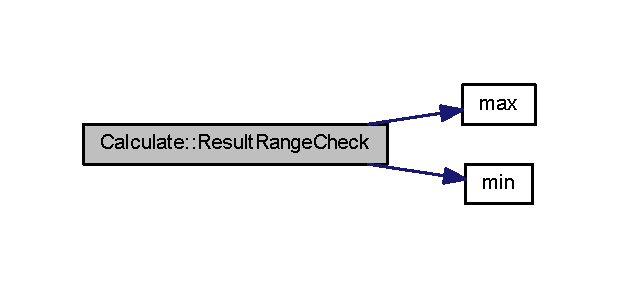
\includegraphics[width=297pt]{class_calculate_a2a0f619344c8154e8740819942ccdddd_cgraph}
\end{center}
\end{figure}


\hypertarget{class_calculate_ab9429972ea44b6d1e57f9bdf7f377e34}{\index{Calculate@{Calculate}!Result\+Range\+Check@{Result\+Range\+Check}}
\index{Result\+Range\+Check@{Result\+Range\+Check}!Calculate@{Calculate}}
\subsubsection[{Result\+Range\+Check}]{\setlength{\rightskip}{0pt plus 5cm}bool Calculate\+::\+Result\+Range\+Check (
\begin{DoxyParamCaption}
\item[{double}]{value\+\_\+1}
\end{DoxyParamCaption}
)\hspace{0.3cm}{\ttfamily [protected]}}}\label{class_calculate_ab9429972ea44b6d1e57f9bdf7f377e34}


Calculate.\+cpp 파일의 312 번째 라인에서 정의되었습니다.


\begin{DoxyCode}
312                                                \{
313     \textcolor{keywordtype}{double} double\_max = \hyperlink{svm_8cpp_a7cba98555a7346b01e4cc06205527d8a}{std::numeric\_limits<double>::max}();
314     \textcolor{keywordtype}{double} double\_min = \hyperlink{svm_8cpp_a348440c5435269ac7c60d2e2d8916f48}{std::numeric\_limits<double>::min}();
315 
316     \textcolor{keywordflow}{if} (value\_1 > double\_max || value\_1 < double\_min)
317         \textcolor{keywordflow}{return} \textcolor{keyword}{false};
318     \textcolor{keywordflow}{else}
319         \textcolor{keywordflow}{return} \textcolor{keyword}{true};
320 \}
\end{DoxyCode}


이 함수 내부에서 호출하는 함수들에 대한 그래프입니다.\+:
\nopagebreak
\begin{figure}[H]
\begin{center}
\leavevmode
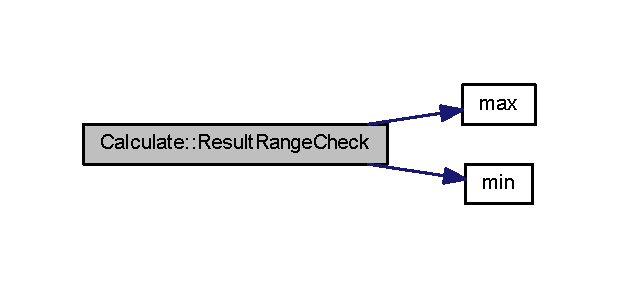
\includegraphics[width=297pt]{class_calculate_ab9429972ea44b6d1e57f9bdf7f377e34_cgraph}
\end{center}
\end{figure}


\hypertarget{class_calculate_a0ad76f7ee31bea1dec46e560d10fca75}{\index{Calculate@{Calculate}!Run@{Run}}
\index{Run@{Run}!Calculate@{Calculate}}
\subsubsection[{Run}]{\setlength{\rightskip}{0pt plus 5cm}double $\ast$ Calculate\+::\+Run (
\begin{DoxyParamCaption}
\item[{String}]{string}
\end{DoxyParamCaption}
)}}\label{class_calculate_a0ad76f7ee31bea1dec46e560d10fca75}


Calculate.\+cpp 파일의 79 번째 라인에서 정의되었습니다.


\begin{DoxyCode}
79                                    \{
80     \hyperlink{class_calculate_aa8f0261822a44685b37dfe22a6eacc04}{Init}();
81 
82     std::string tempstring;
83     tempstring = \hyperlink{class_calculate_a50d0dfb999edd48ae45b8023e6a69d6a}{Calculate::WStringtostring}(input);
84     \textcolor{keyword}{const} \textcolor{keywordtype}{char}* \textcolor{keywordtype}{string} = tempstring.c\_str();
85 
86     \textcolor{keywordflow}{if} (!\hyperlink{class_calculate_a680527f598a4b37febfcdeb21dea6e9c}{Read}(\textcolor{keywordtype}{string})) \{
87         printf(\textcolor{stringliteral}{"   Error : Unpaired bracket...!\(\backslash\)n"});
88         \textcolor{keywordflow}{return} NULL;
89     \}
90 
91     \hyperlink{class_calculate_a81090066a9bc2e77432198e45850eb5d}{Postfix}();
92     \hyperlink{class_calculate_af81d8f0097a86c858825c3deef573697}{Evaluate}();
93 
94     \textcolor{keywordflow}{return} \hyperlink{class_calculate_a5ffe97b9c4358acf90360d328b9144c0}{m\_fResult};
95 \}
\end{DoxyCode}


이 함수 내부에서 호출하는 함수들에 대한 그래프입니다.\+:
\nopagebreak
\begin{figure}[H]
\begin{center}
\leavevmode
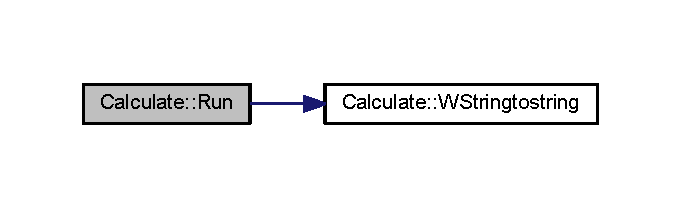
\includegraphics[width=327pt]{class_calculate_a0ad76f7ee31bea1dec46e560d10fca75_cgraph}
\end{center}
\end{figure}




이 함수를 호출하는 함수들에 대한 그래프입니다.\+:
\nopagebreak
\begin{figure}[H]
\begin{center}
\leavevmode
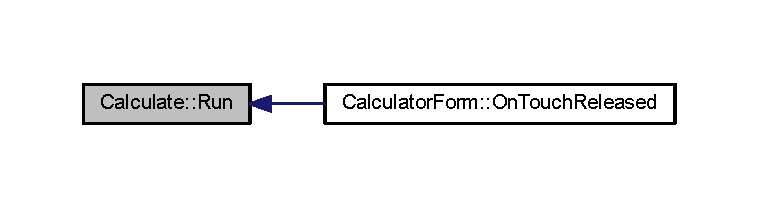
\includegraphics[width=350pt]{class_calculate_a0ad76f7ee31bea1dec46e560d10fca75_icgraph}
\end{center}
\end{figure}


\hypertarget{class_calculate_a50d0dfb999edd48ae45b8023e6a69d6a}{\index{Calculate@{Calculate}!W\+Stringtostring@{W\+Stringtostring}}
\index{W\+Stringtostring@{W\+Stringtostring}!Calculate@{Calculate}}
\subsubsection[{W\+Stringtostring}]{\setlength{\rightskip}{0pt plus 5cm}std\+::string Calculate\+::\+W\+Stringtostring (
\begin{DoxyParamCaption}
\item[{Tizen\+::\+Base\+::\+String}]{input}
\end{DoxyParamCaption}
)}}\label{class_calculate_a50d0dfb999edd48ae45b8023e6a69d6a}


Calculate.\+cpp 파일의 102 번째 라인에서 정의되었습니다.


\begin{DoxyCode}
102                                                           \{
103     std::string after;
104     std::wstring before(input.GetPointer());
105     after.assign(before.begin(), before.end());
106 
107     \textcolor{keywordflow}{return} after.c\_str();
108 \}
\end{DoxyCode}


이 함수를 호출하는 함수들에 대한 그래프입니다.\+:
\nopagebreak
\begin{figure}[H]
\begin{center}
\leavevmode
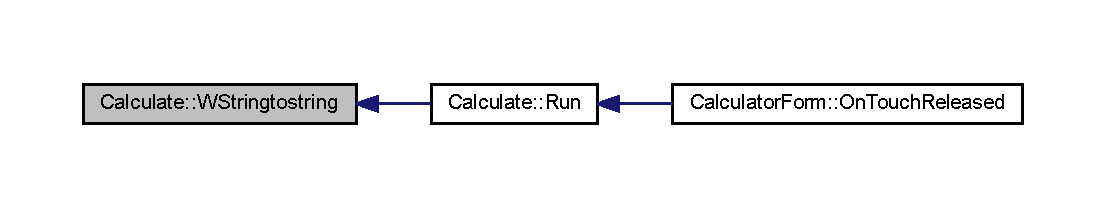
\includegraphics[width=350pt]{class_calculate_a50d0dfb999edd48ae45b8023e6a69d6a_icgraph}
\end{center}
\end{figure}




\subsection{멤버 데이타 문서화}
\hypertarget{class_calculate_a91ed53268a8f29f54757037bc28d35e0}{\index{Calculate@{Calculate}!m\+\_\+b\+Mode@{m\+\_\+b\+Mode}}
\index{m\+\_\+b\+Mode@{m\+\_\+b\+Mode}!Calculate@{Calculate}}
\subsubsection[{m\+\_\+b\+Mode}]{\setlength{\rightskip}{0pt plus 5cm}{\bf B\+O\+O\+L} Calculate\+::m\+\_\+b\+Mode\hspace{0.3cm}{\ttfamily [protected]}}}\label{class_calculate_a91ed53268a8f29f54757037bc28d35e0}


Calculate.\+h 파일의 32 번째 라인에서 정의되었습니다.

\hypertarget{class_calculate_a5ffe97b9c4358acf90360d328b9144c0}{\index{Calculate@{Calculate}!m\+\_\+f\+Result@{m\+\_\+f\+Result}}
\index{m\+\_\+f\+Result@{m\+\_\+f\+Result}!Calculate@{Calculate}}
\subsubsection[{m\+\_\+f\+Result}]{\setlength{\rightskip}{0pt plus 5cm}double$\ast$ Calculate\+::m\+\_\+f\+Result\hspace{0.3cm}{\ttfamily [protected]}}}\label{class_calculate_a5ffe97b9c4358acf90360d328b9144c0}


Calculate.\+h 파일의 35 번째 라인에서 정의되었습니다.

\hypertarget{class_calculate_a7ded18ea2282684cf9570cceadbcbf37}{\index{Calculate@{Calculate}!m\+\_\+f\+Value@{m\+\_\+f\+Value}}
\index{m\+\_\+f\+Value@{m\+\_\+f\+Value}!Calculate@{Calculate}}
\subsubsection[{m\+\_\+f\+Value}]{\setlength{\rightskip}{0pt plus 5cm}double$\ast$ Calculate\+::m\+\_\+f\+Value\hspace{0.3cm}{\ttfamily [protected]}}}\label{class_calculate_a7ded18ea2282684cf9570cceadbcbf37}


Calculate.\+h 파일의 38 번째 라인에서 정의되었습니다.

\hypertarget{class_calculate_ae2a302680f654bfa735b1dc4f34814b6}{\index{Calculate@{Calculate}!m\+\_\+n\+Stack@{m\+\_\+n\+Stack}}
\index{m\+\_\+n\+Stack@{m\+\_\+n\+Stack}!Calculate@{Calculate}}
\subsubsection[{m\+\_\+n\+Stack}]{\setlength{\rightskip}{0pt plus 5cm}int$\ast$ Calculate\+::m\+\_\+n\+Stack\hspace{0.3cm}{\ttfamily [protected]}}}\label{class_calculate_ae2a302680f654bfa735b1dc4f34814b6}


Calculate.\+h 파일의 37 번째 라인에서 정의되었습니다.

\hypertarget{class_calculate_a9f6afe7d8278100e1f27977aaeba0a72}{\index{Calculate@{Calculate}!m\+\_\+n\+Top@{m\+\_\+n\+Top}}
\index{m\+\_\+n\+Top@{m\+\_\+n\+Top}!Calculate@{Calculate}}
\subsubsection[{m\+\_\+n\+Top}]{\setlength{\rightskip}{0pt plus 5cm}int Calculate\+::m\+\_\+n\+Top\hspace{0.3cm}{\ttfamily [protected]}}}\label{class_calculate_a9f6afe7d8278100e1f27977aaeba0a72}


Calculate.\+h 파일의 36 번째 라인에서 정의되었습니다.

\hypertarget{class_calculate_a1b964b49f9a186fa02643c1361ccd4ab}{\index{Calculate@{Calculate}!m\+\_\+str\+Infix@{m\+\_\+str\+Infix}}
\index{m\+\_\+str\+Infix@{m\+\_\+str\+Infix}!Calculate@{Calculate}}
\subsubsection[{m\+\_\+str\+Infix}]{\setlength{\rightskip}{0pt plus 5cm}char$\ast$ Calculate\+::m\+\_\+str\+Infix\hspace{0.3cm}{\ttfamily [protected]}}}\label{class_calculate_a1b964b49f9a186fa02643c1361ccd4ab}


Calculate.\+h 파일의 39 번째 라인에서 정의되었습니다.

\hypertarget{class_calculate_aceafe6d40cd154f9535dc971c1e9bb7a}{\index{Calculate@{Calculate}!m\+\_\+str\+Postfix@{m\+\_\+str\+Postfix}}
\index{m\+\_\+str\+Postfix@{m\+\_\+str\+Postfix}!Calculate@{Calculate}}
\subsubsection[{m\+\_\+str\+Postfix}]{\setlength{\rightskip}{0pt plus 5cm}char$\ast$ Calculate\+::m\+\_\+str\+Postfix\hspace{0.3cm}{\ttfamily [protected]}}}\label{class_calculate_aceafe6d40cd154f9535dc971c1e9bb7a}


Calculate.\+h 파일의 40 번째 라인에서 정의되었습니다.

\hypertarget{class_calculate_a75fc03f230ef600e36be8073acc34216}{\index{Calculate@{Calculate}!Variable@{Variable}}
\index{Variable@{Variable}!Calculate@{Calculate}}
\subsubsection[{Variable}]{\setlength{\rightskip}{0pt plus 5cm}double Calculate\+::\+Variable\hspace{0.3cm}{\ttfamily [static]}, {\ttfamily [protected]}}}\label{class_calculate_a75fc03f230ef600e36be8073acc34216}
{\bfseries 초기값\+:}
\begin{DoxyCode}
= \{ \textcolor{charliteral}{'\(\backslash\)r'}, \textcolor{charliteral}{'\(\backslash\)r'}, \textcolor{charliteral}{'\(\backslash\)r'}, \textcolor{charliteral}{'\(\backslash\)r'}, \textcolor{charliteral}{'\(\backslash\)r'}, \textcolor{charliteral}{'\(\backslash\)r'}, \textcolor{charliteral}{'\(\backslash\)r'},
        \textcolor{charliteral}{'\(\backslash\)r'}, \textcolor{charliteral}{'\(\backslash\)r'}, \textcolor{charliteral}{'\(\backslash\)r'}, \textcolor{charliteral}{'\(\backslash\)r'}, \textcolor{charliteral}{'\(\backslash\)r'}, \textcolor{charliteral}{'\(\backslash\)r'}, \textcolor{charliteral}{'\(\backslash\)r'}, \textcolor{charliteral}{'\(\backslash\)r'}, \textcolor{charliteral}{'\(\backslash\)r'}, \textcolor{charliteral}{'\(\backslash\)r'}, \textcolor{charliteral}{'\(\backslash\)r'}, \textcolor{charliteral}{'\(\backslash\)r'},
        \textcolor{charliteral}{'\(\backslash\)r'}, \textcolor{charliteral}{'\(\backslash\)r'}, \textcolor{charliteral}{'\(\backslash\)r'}, \textcolor{charliteral}{'\(\backslash\)r'}, \textcolor{charliteral}{'\(\backslash\)r'}, \textcolor{charliteral}{'\(\backslash\)r'}, \textcolor{charliteral}{'\(\backslash\)r'}, \}
\end{DoxyCode}


Calculate.\+h 파일의 31 번째 라인에서 정의되었습니다.



이 클래스에 대한 문서화 페이지는 다음의 파일들로부터 생성되었습니다.\+:\begin{DoxyCompactItemize}
\item 
inc/\hyperlink{_calculate_8h}{Calculate.\+h}\item 
src/\+Calculator/\hyperlink{_calculate_8cpp}{Calculate.\+cpp}\end{DoxyCompactItemize}

\hypertarget{class_calculator_form}{\section{Calculator\+Form 클래스 참조}
\label{class_calculator_form}\index{Calculator\+Form@{Calculator\+Form}}
}


Calculator Form을 구성해주는 Class.  




{\ttfamily \#include $<$Calculator\+Form.\+h$>$}



Calculator\+Form에 대한 상속 다이어그램 \+: 
\nopagebreak
\begin{figure}[H]
\begin{center}
\leavevmode
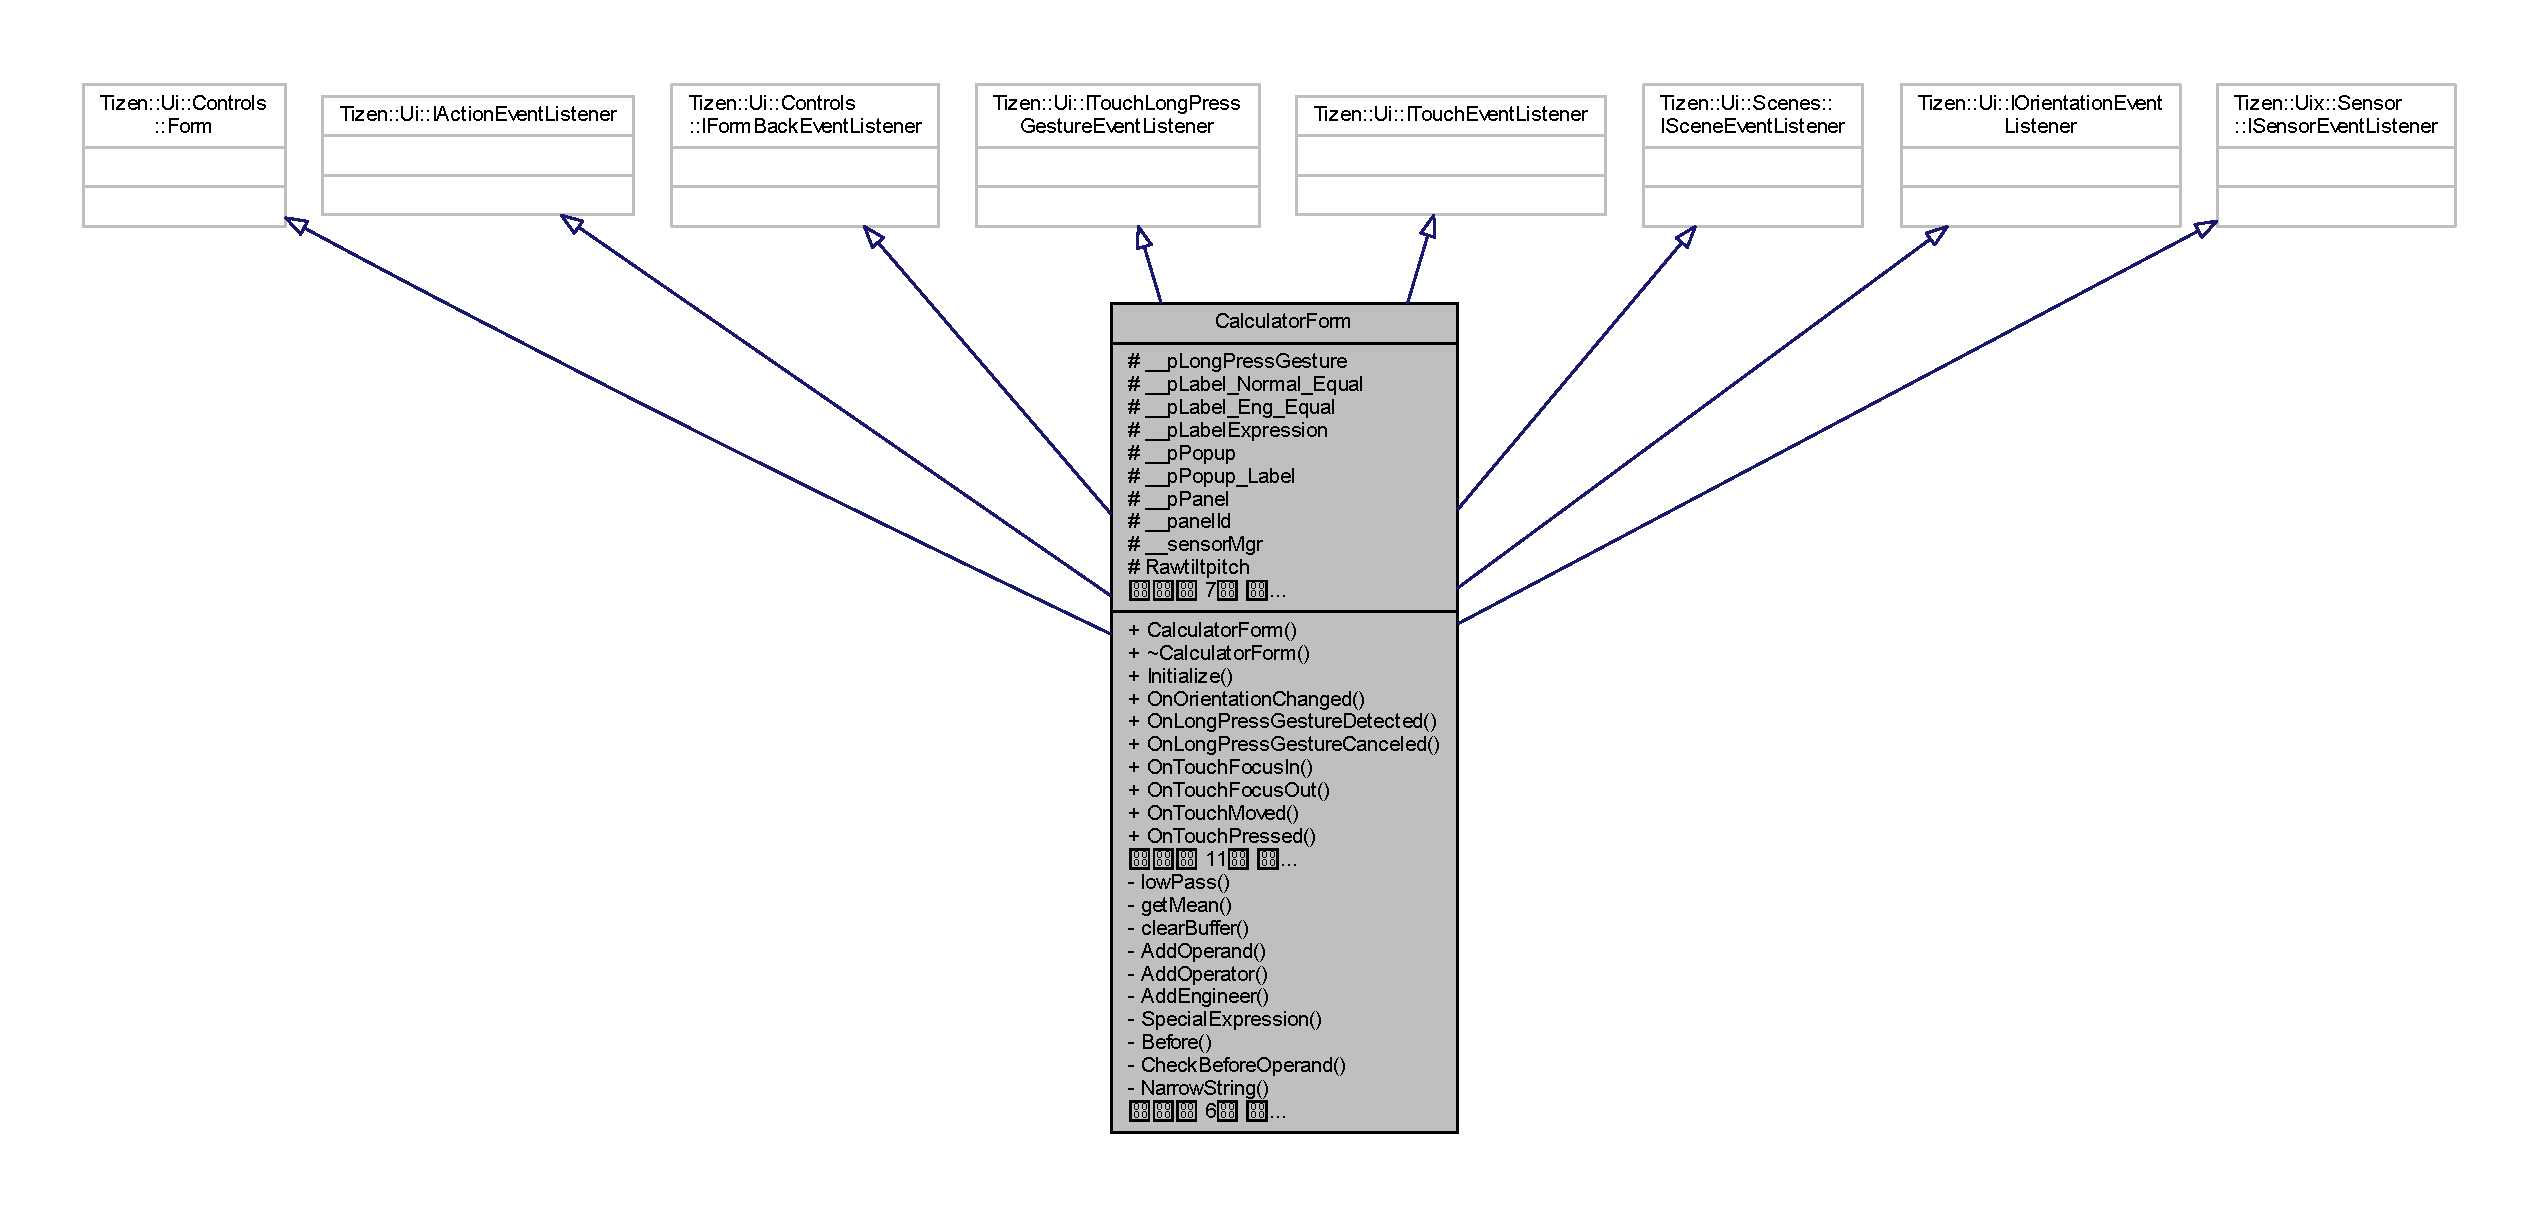
\includegraphics[width=350pt]{class_calculator_form__inherit__graph}
\end{center}
\end{figure}


Calculator\+Form에 대한 협력 다이어그램\+:
\nopagebreak
\begin{figure}[H]
\begin{center}
\leavevmode
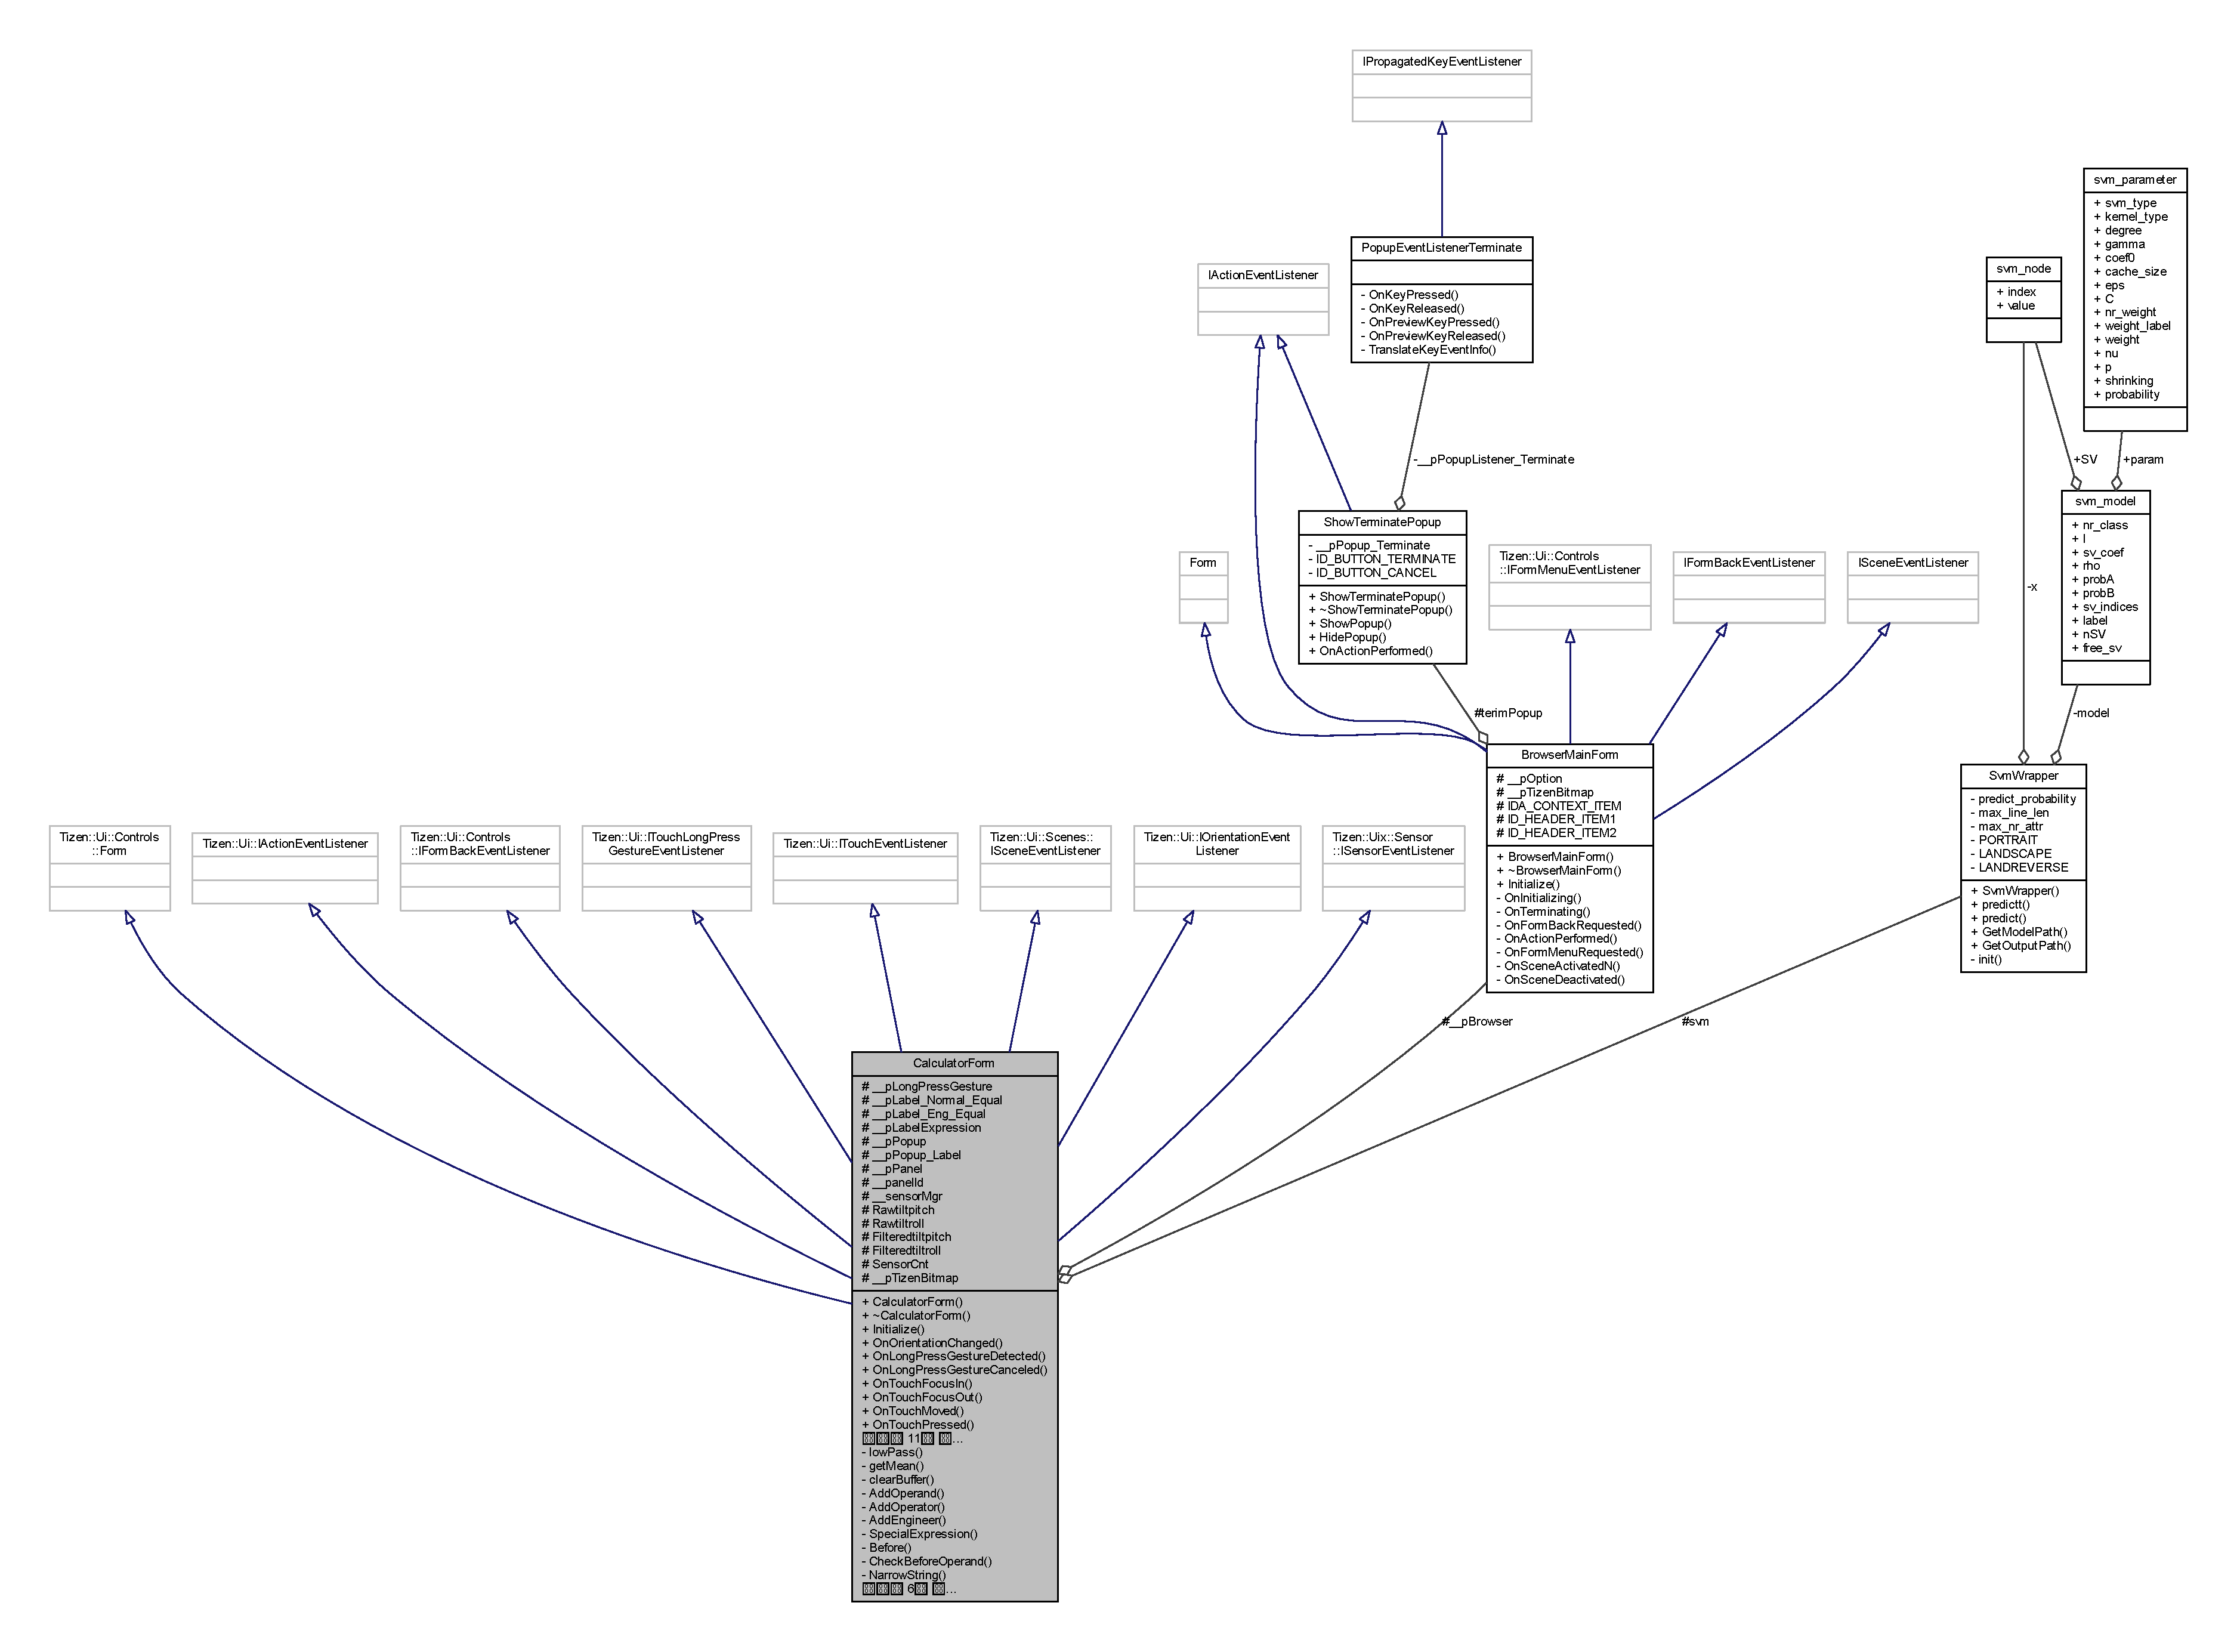
\includegraphics[width=350pt]{class_calculator_form__coll__graph}
\end{center}
\end{figure}
\subsection*{Public 멤버 함수}
\begin{DoxyCompactItemize}
\item 
\hyperlink{class_calculator_form_a9ca53c4d95d365be85a7d1c722eb4eaf}{Calculator\+Form} (void)
\item 
virtual \hyperlink{class_calculator_form_a4287a4a56574e3d7153629e9032b7519}{$\sim$\+Calculator\+Form} (void)
\item 
bool \hyperlink{class_calculator_form_a51137823626f92e48605c6d9aa2e220f}{Initialize} ()
\item 
void \hyperlink{class_calculator_form_ac298449ce5bedae6a69ccd2f13594ce2}{On\+Orientation\+Changed} (const Tizen\+::\+Ui\+::\+Control \&source, Tizen\+::\+Ui\+::\+Orientation\+Status orientation\+Status)
\item 
virtual void \hyperlink{class_calculator_form_a636fe70d8357bc09e2404227a8fbc6d7}{On\+Long\+Press\+Gesture\+Detected} (Tizen\+::\+Ui\+::\+Touch\+Long\+Press\+Gesture\+Detector \&gesture\+Detector)
\item 
virtual void \hyperlink{class_calculator_form_acd85d807e5b1033d588828dc4685c021}{On\+Long\+Press\+Gesture\+Canceled} (Tizen\+::\+Ui\+::\+Touch\+Long\+Press\+Gesture\+Detector \&gesture\+Detector)
\item 
virtual void \hyperlink{class_calculator_form_a7605c35fa6faaadbce71705c19403907}{On\+Touch\+Focus\+In} (const Tizen\+::\+Ui\+::\+Control \&source, const Tizen\+::\+Graphics\+::\+Point \&current\+Position, const Tizen\+::\+Ui\+::\+Touch\+Event\+Info \&touch\+Info)
\item 
virtual void \hyperlink{class_calculator_form_a3d05f489ea3b0417143c6824642299b8}{On\+Touch\+Focus\+Out} (const Tizen\+::\+Ui\+::\+Control \&source, const Tizen\+::\+Graphics\+::\+Point \&current\+Position, const Tizen\+::\+Ui\+::\+Touch\+Event\+Info \&touch\+Info)
\item 
virtual void \hyperlink{class_calculator_form_ac710421b5902c784ffc1dd853d0b9036}{On\+Touch\+Moved} (const Tizen\+::\+Ui\+::\+Control \&source, const Tizen\+::\+Graphics\+::\+Point \&current\+Position, const Tizen\+::\+Ui\+::\+Touch\+Event\+Info \&touch\+Info)
\item 
virtual void \hyperlink{class_calculator_form_ae0cae03d37d3913bbe0971ad997af4e5}{On\+Touch\+Pressed} (const Tizen\+::\+Ui\+::\+Control \&source, const Tizen\+::\+Graphics\+::\+Point \&current\+Position, const Tizen\+::\+Ui\+::\+Touch\+Event\+Info \&touch\+Info)
\item 
virtual void \hyperlink{class_calculator_form_ab270921ccfd02b9dc7da04b5568cae4e}{On\+Touch\+Released} (const Tizen\+::\+Ui\+::\+Control \&source, const Tizen\+::\+Graphics\+::\+Point \&current\+Position, const Tizen\+::\+Ui\+::\+Touch\+Event\+Info \&touch\+Info)
\item 
virtual void \hyperlink{class_calculator_form_a65cd7728c92b73141787a9c2333462d7}{On\+Data\+Received} (Tizen\+::\+Uix\+::\+Sensor\+::\+Sensor\+Type sensor\+Type, Tizen\+::\+Uix\+::\+Sensor\+::\+Sensor\+Data \&sensor\+Data, result r)
\item 
void \hyperlink{class_calculator_form_afaa8fab392f2dd958cab631e4a2c019f}{Start\+Sensor} (void)
\item 
void \hyperlink{class_calculator_form_a2ea52e1ac047a01188384b416d41c461}{Stop\+Sensor} (void)
\item 
void \hyperlink{class_calculator_form_ae739bb0f8aea14c0ae2d440950130bc2}{Feature\+Processing} (void)
\item 
virtual void \hyperlink{class_calculator_form_afbb0a77caee4d2686ea67ad41a4d431e}{On\+Scene\+Activated\+N} (const Tizen\+::\+Ui\+::\+Scenes\+::\+Scene\+Id \&previous\+Scene\+Id, const Tizen\+::\+Ui\+::\+Scenes\+::\+Scene\+Id \&current\+Scene\+Id, Tizen\+::\+Base\+::\+Collection\+::\+I\+List $\ast$p\+Args)
\item 
virtual void \hyperlink{class_calculator_form_af4b6ee4f7baaec70259f2d631d3152e8}{On\+Scene\+Deactivated} (const Tizen\+::\+Ui\+::\+Scenes\+::\+Scene\+Id \&current\+Scene\+Id, const Tizen\+::\+Ui\+::\+Scenes\+::\+Scene\+Id \&next\+Scene\+Id)
\item 
virtual result \hyperlink{class_calculator_form_a6ffeb117d9770054839979bd5d81913e}{On\+Initializing} (void)
\item 
virtual result \hyperlink{class_calculator_form_a157ce99572a803a9a5638e0a6d60518a}{On\+Terminating} (void)
\item 
virtual void \hyperlink{class_calculator_form_a3736d53b1ad6388353463511485750cf}{On\+Form\+Back\+Requested} (Tizen\+::\+Ui\+::\+Controls\+::\+Form \&source)
\item 
virtual void \hyperlink{class_calculator_form_af30252093893f4cb4d5578e919d3381f}{On\+Action\+Performed} (const Tizen\+::\+Ui\+::\+Control \&source, int action\+Id)
\end{DoxyCompactItemize}
\subsection*{Protected 속성}
\begin{DoxyCompactItemize}
\item 
Tizen\+::\+Ui\+::\+Touch\+Long\+Press\+Gesture\+Detector $\ast$ \hyperlink{class_calculator_form_ae2c4d24712fa767d536ffc901810bff3}{\+\_\+\+\_\+p\+Long\+Press\+Gesture}
\item 
Tizen\+::\+Ui\+::\+Controls\+::\+Label $\ast$ \hyperlink{class_calculator_form_ae9a8c51bc39c7ec66a7e43f6c29a14d8}{\+\_\+\+\_\+p\+Label\+\_\+\+Normal\+\_\+\+Equal}
\item 
Tizen\+::\+Ui\+::\+Controls\+::\+Label $\ast$ \hyperlink{class_calculator_form_a57055baa16d93e319c193d01bf833bc7}{\+\_\+\+\_\+p\+Label\+\_\+\+Eng\+\_\+\+Equal}
\item 
Tizen\+::\+Ui\+::\+Controls\+::\+Label $\ast$ \hyperlink{class_calculator_form_a85c791f34a8b69e7d22b7d64d7f69bac}{\+\_\+\+\_\+p\+Label\+Expression}
\item 
Tizen\+::\+Ui\+::\+Controls\+::\+Popup $\ast$ \hyperlink{class_calculator_form_aa22a98e80f0533746ca5c712ea3b7a8e}{\+\_\+\+\_\+p\+Popup}
\item 
Tizen\+::\+Ui\+::\+Controls\+::\+Label $\ast$ \hyperlink{class_calculator_form_aabf0dd69d2567ee96db776f4bbe53f4e}{\+\_\+\+\_\+p\+Popup\+\_\+\+Label}
\item 
Tizen\+::\+Ui\+::\+Controls\+::\+Panel $\ast$ \hyperlink{class_calculator_form_ae930aeea4ccaf0fd752c11350c6e2af6}{\+\_\+\+\_\+p\+Panel} \mbox{[}2\mbox{]}
\item 
int \hyperlink{class_calculator_form_a4b8ee8d07acfddbe9140a17a37b23109}{\+\_\+\+\_\+panel\+Id}
\item 
Tizen\+::\+Uix\+::\+Sensor\+::\+Sensor\+Manager \hyperlink{class_calculator_form_abb49d4c96119ee3adaf6a9bf8302ddaa}{\+\_\+\+\_\+sensor\+Mgr}
\item 
Tizen\+::\+Base\+::\+Collection\+::\+Array\+List\+T\\*
$<$ float $>$ \hyperlink{class_calculator_form_a7b784d40a3d83eee41bb8efae09142ca}{Rawtiltpitch}
\item 
Tizen\+::\+Base\+::\+Collection\+::\+Array\+List\+T\\*
$<$ float $>$ \hyperlink{class_calculator_form_afc8797d0cb7657a384ccc03c7f335aed}{Rawtiltroll}
\item 
Tizen\+::\+Base\+::\+Collection\+::\+Array\+List\+T\\*
$<$ float $>$ \hyperlink{class_calculator_form_a54065fa7531b14c744c8d11ccd849f81}{Filteredtiltpitch}
\item 
Tizen\+::\+Base\+::\+Collection\+::\+Array\+List\+T\\*
$<$ float $>$ \hyperlink{class_calculator_form_a63438d1ef5396e2d216eaf604659c96c}{Filteredtiltroll}
\item 
\hyperlink{class_svm_wrapper}{Svm\+Wrapper} \hyperlink{class_calculator_form_ac3e3da16eada2566553b992a8d254366}{svm}
\item 
int \hyperlink{class_calculator_form_a846432327af7a8d40a4a3b586ee3581a}{Sensor\+Cnt}
\item 
\hyperlink{class_browser_main_form}{Browser\+Main\+Form} $\ast$ \hyperlink{class_calculator_form_afc760fc5946b899bd2b0807157098a3e}{\+\_\+\+\_\+p\+Browser}
\item 
Tizen\+::\+Graphics\+::\+Bitmap $\ast$ \hyperlink{class_calculator_form_a88ec1e4da579824a2f78534d11ffad8b}{\+\_\+\+\_\+p\+Tizen\+Bitmap}
\end{DoxyCompactItemize}
\subsection*{Private 타입}
\begin{DoxyCompactItemize}
\item 
enum \hyperlink{class_calculator_form_a7f0486405077c1eaee1faa73e631a67f}{Button\+Action\+Id} \{ \\*
\hyperlink{class_calculator_form_a7f0486405077c1eaee1faa73e631a67fa36847135c8b46dba3738ae1fdb7e3706}{I\+D\+\_\+\+N\+O\+R\+\_\+\+B\+T\+N\+\_\+0}, 
\hyperlink{class_calculator_form_a7f0486405077c1eaee1faa73e631a67facb654bf70d6d1c0f2ba3a51e7f54bcec}{I\+D\+\_\+\+N\+O\+R\+\_\+\+B\+T\+N\+\_\+1}, 
\hyperlink{class_calculator_form_a7f0486405077c1eaee1faa73e631a67fa5979614c050c3bcb0b3ac03c81cfbd71}{I\+D\+\_\+\+N\+O\+R\+\_\+\+B\+T\+N\+\_\+2}, 
\hyperlink{class_calculator_form_a7f0486405077c1eaee1faa73e631a67fa276bf31b6dff33ed4cbb573b2f821cdb}{I\+D\+\_\+\+N\+O\+R\+\_\+\+B\+T\+N\+\_\+3}, 
\\*
\hyperlink{class_calculator_form_a7f0486405077c1eaee1faa73e631a67fa74bce332df52efead67e481025bd68e6}{I\+D\+\_\+\+N\+O\+R\+\_\+\+B\+T\+N\+\_\+4}, 
\hyperlink{class_calculator_form_a7f0486405077c1eaee1faa73e631a67fa6a71324302629d7b14f8aa6a69b18ecc}{I\+D\+\_\+\+N\+O\+R\+\_\+\+B\+T\+N\+\_\+5}, 
\hyperlink{class_calculator_form_a7f0486405077c1eaee1faa73e631a67fa6645c0b47b7414fbaf95efcdab161c83}{I\+D\+\_\+\+N\+O\+R\+\_\+\+B\+T\+N\+\_\+6}, 
\hyperlink{class_calculator_form_a7f0486405077c1eaee1faa73e631a67fa079f3395882ff05ebdab30a802a948af}{I\+D\+\_\+\+N\+O\+R\+\_\+\+B\+T\+N\+\_\+7}, 
\\*
\hyperlink{class_calculator_form_a7f0486405077c1eaee1faa73e631a67fa94f50ff40314d7f9580755252fefe510}{I\+D\+\_\+\+N\+O\+R\+\_\+\+B\+T\+N\+\_\+8}, 
\hyperlink{class_calculator_form_a7f0486405077c1eaee1faa73e631a67fa0a4fbbd355bdae0d35fbc895aa177ced}{I\+D\+\_\+\+N\+O\+R\+\_\+\+B\+T\+N\+\_\+9}, 
\hyperlink{class_calculator_form_a7f0486405077c1eaee1faa73e631a67fa25ee67c6b962363d0600656387ac01d4}{I\+D\+\_\+\+N\+O\+R\+\_\+\+B\+T\+N\+\_\+\+D\+O\+T}, 
\hyperlink{class_calculator_form_a7f0486405077c1eaee1faa73e631a67fa11735001f5ed24c041d279719871d922}{I\+D\+\_\+\+N\+O\+R\+\_\+\+B\+T\+N\+\_\+\+S\+I\+G\+N}, 
\\*
\hyperlink{class_calculator_form_a7f0486405077c1eaee1faa73e631a67fa399bc7ab7ecdeb3e2160376c94e59b6a}{I\+D\+\_\+\+N\+O\+R\+\_\+\+B\+T\+N\+\_\+\+M\+I\+N\+U\+S}, 
\hyperlink{class_calculator_form_a7f0486405077c1eaee1faa73e631a67faa5b58117f4dd98124b55dd697ab2bb5a}{I\+D\+\_\+\+N\+O\+R\+\_\+\+B\+T\+N\+\_\+\+P\+L\+U\+S}, 
\hyperlink{class_calculator_form_a7f0486405077c1eaee1faa73e631a67faaf29ed3ab5f682dcc72923e64fc5327a}{I\+D\+\_\+\+N\+O\+R\+\_\+\+B\+T\+N\+\_\+\+B\+A\+C\+K}, 
\hyperlink{class_calculator_form_a7f0486405077c1eaee1faa73e631a67fabac2fde992d2d7d97ffcbd7f21352d4c}{I\+D\+\_\+\+N\+O\+R\+\_\+\+B\+T\+N\+\_\+\+M\+U\+L\+T\+I\+P\+L\+Y}, 
\\*
\hyperlink{class_calculator_form_a7f0486405077c1eaee1faa73e631a67fac05e591891daa63c36e391a458b012b2}{I\+D\+\_\+\+N\+O\+R\+\_\+\+B\+T\+N\+\_\+\+D\+I\+V\+I\+D\+E}, 
\hyperlink{class_calculator_form_a7f0486405077c1eaee1faa73e631a67fa68cc91926a6e943b65d800e718a7e8fd}{I\+D\+\_\+\+N\+O\+R\+\_\+\+B\+T\+N\+\_\+\+P\+A\+R\+E\+N}, 
\hyperlink{class_calculator_form_a7f0486405077c1eaee1faa73e631a67fab02a04ef035999b7ed04fb31c1c64501}{I\+D\+\_\+\+N\+O\+R\+\_\+\+B\+T\+N\+\_\+\+C\+L\+E\+A\+R}, 
\hyperlink{class_calculator_form_a7f0486405077c1eaee1faa73e631a67fada58ff2bcae312b4d937de88c5e6392d}{I\+D\+\_\+\+E\+N\+G\+\_\+\+B\+T\+N\+\_\+0}, 
\\*
\hyperlink{class_calculator_form_a7f0486405077c1eaee1faa73e631a67faa2fca2ce7488b16e9ab0154485af5474}{I\+D\+\_\+\+E\+N\+G\+\_\+\+B\+T\+N\+\_\+1}, 
\hyperlink{class_calculator_form_a7f0486405077c1eaee1faa73e631a67fa04f038704039c1943995dedb16a1dec2}{I\+D\+\_\+\+E\+N\+G\+\_\+\+B\+T\+N\+\_\+2}, 
\hyperlink{class_calculator_form_a7f0486405077c1eaee1faa73e631a67fa9dbb058cd33957c0e3f3432515a59f5f}{I\+D\+\_\+\+E\+N\+G\+\_\+\+B\+T\+N\+\_\+3}, 
\hyperlink{class_calculator_form_a7f0486405077c1eaee1faa73e631a67facaa578f61ab27a654264de100a480254}{I\+D\+\_\+\+E\+N\+G\+\_\+\+B\+T\+N\+\_\+4}, 
\\*
\hyperlink{class_calculator_form_a7f0486405077c1eaee1faa73e631a67fa02fb238b0c78356f31d71f4028c2a966}{I\+D\+\_\+\+E\+N\+G\+\_\+\+B\+T\+N\+\_\+5}, 
\hyperlink{class_calculator_form_a7f0486405077c1eaee1faa73e631a67fa437b9321c7aa469549ed4c3a2d0a44d4}{I\+D\+\_\+\+E\+N\+G\+\_\+\+B\+T\+N\+\_\+6}, 
\hyperlink{class_calculator_form_a7f0486405077c1eaee1faa73e631a67fa1ce33b8c2b0834d0b3c611b2a0be81d4}{I\+D\+\_\+\+E\+N\+G\+\_\+\+B\+T\+N\+\_\+7}, 
\hyperlink{class_calculator_form_a7f0486405077c1eaee1faa73e631a67fa3b47082c5d91658d924c744f2aa718a5}{I\+D\+\_\+\+E\+N\+G\+\_\+\+B\+T\+N\+\_\+8}, 
\\*
\hyperlink{class_calculator_form_a7f0486405077c1eaee1faa73e631a67fa8d9bbd7046fa548f53cf7d5637804082}{I\+D\+\_\+\+E\+N\+G\+\_\+\+B\+T\+N\+\_\+9}, 
\hyperlink{class_calculator_form_a7f0486405077c1eaee1faa73e631a67fad221bcacd57dc62d8c24a8bea9550337}{I\+D\+\_\+\+E\+N\+G\+\_\+\+B\+T\+N\+\_\+\+D\+O\+T}, 
\hyperlink{class_calculator_form_a7f0486405077c1eaee1faa73e631a67faa0129118f616b983e0815c27633338bf}{I\+D\+\_\+\+E\+N\+G\+\_\+\+B\+T\+N\+\_\+\+S\+I\+G\+N}, 
\hyperlink{class_calculator_form_a7f0486405077c1eaee1faa73e631a67fa0b2145bcc8d621a0813d82172311ce3f}{I\+D\+\_\+\+E\+N\+G\+\_\+\+B\+T\+N\+\_\+\+M\+I\+N\+U\+S}, 
\\*
\hyperlink{class_calculator_form_a7f0486405077c1eaee1faa73e631a67fa7e49dbbe01a555e1cdc467a31d6646c5}{I\+D\+\_\+\+E\+N\+G\+\_\+\+B\+T\+N\+\_\+\+P\+L\+U\+S}, 
\hyperlink{class_calculator_form_a7f0486405077c1eaee1faa73e631a67fa845c87456de70101a96f1a6f1aedcc75}{I\+D\+\_\+\+E\+N\+G\+\_\+\+B\+T\+N\+\_\+\+B\+A\+C\+K}, 
\hyperlink{class_calculator_form_a7f0486405077c1eaee1faa73e631a67face617b5a3f58f07423eea9111b63132e}{I\+D\+\_\+\+E\+N\+G\+\_\+\+B\+T\+N\+\_\+\+M\+U\+L\+T\+I\+P\+L\+Y}, 
\hyperlink{class_calculator_form_a7f0486405077c1eaee1faa73e631a67fa23fcaaf8e46bd3ee549352e7233af15e}{I\+D\+\_\+\+E\+N\+G\+\_\+\+B\+T\+N\+\_\+\+D\+I\+V\+I\+D\+E}, 
\\*
\hyperlink{class_calculator_form_a7f0486405077c1eaee1faa73e631a67fa437a7542ade59a274923fdf9d68688bc}{I\+D\+\_\+\+E\+N\+G\+\_\+\+B\+T\+N\+\_\+\+P\+A\+R\+E\+N}, 
\hyperlink{class_calculator_form_a7f0486405077c1eaee1faa73e631a67fa7f5a292d77802a52f1ea91dcfab03756}{I\+D\+\_\+\+E\+N\+G\+\_\+\+B\+T\+N\+\_\+\+C\+L\+E\+A\+R}, 
\hyperlink{class_calculator_form_a7f0486405077c1eaee1faa73e631a67fabf47eac7bede8b3614af465f83944d25}{I\+D\+\_\+\+E\+N\+G\+\_\+\+B\+T\+N\+\_\+\+F\+A\+C\+T\+O}, 
\hyperlink{class_calculator_form_a7f0486405077c1eaee1faa73e631a67fab0b134c86cd90127e3cb02328260bf95}{I\+D\+\_\+\+E\+N\+G\+\_\+\+B\+T\+N\+\_\+\+R\+O\+O\+T}, 
\\*
\hyperlink{class_calculator_form_a7f0486405077c1eaee1faa73e631a67fafafc4a31d9c1a9d5333f09bf852bbe3f}{I\+D\+\_\+\+E\+N\+G\+\_\+\+B\+T\+N\+\_\+\+P\+E\+R\+C\+E\+N\+T}, 
\hyperlink{class_calculator_form_a7f0486405077c1eaee1faa73e631a67faa0899f6f1819e97246d4a2e7d638b14c}{I\+D\+\_\+\+E\+N\+G\+\_\+\+B\+T\+N\+\_\+\+S\+I\+N}, 
\hyperlink{class_calculator_form_a7f0486405077c1eaee1faa73e631a67faa0fb52e70f50596259fecf8e0ce037f5}{I\+D\+\_\+\+E\+N\+G\+\_\+\+B\+T\+N\+\_\+\+C\+O\+S}, 
\hyperlink{class_calculator_form_a7f0486405077c1eaee1faa73e631a67faf99e3f69403a41412e639c269fcc87d3}{I\+D\+\_\+\+E\+N\+G\+\_\+\+B\+T\+N\+\_\+\+T\+A\+N}, 
\\*
\hyperlink{class_calculator_form_a7f0486405077c1eaee1faa73e631a67fa72adc19c50013f5027bcccf22006d5d0}{I\+D\+\_\+\+E\+N\+G\+\_\+\+B\+T\+N\+\_\+\+L\+N}, 
\hyperlink{class_calculator_form_a7f0486405077c1eaee1faa73e631a67fa1ba8354f2bf98fd0c011f877c0bef4d9}{I\+D\+\_\+\+E\+N\+G\+\_\+\+B\+T\+N\+\_\+\+L\+O\+G}, 
\hyperlink{class_calculator_form_a7f0486405077c1eaee1faa73e631a67faed97aeab42c4fca6d34e26919f897f9b}{I\+D\+\_\+\+E\+N\+G\+\_\+\+B\+T\+N\+\_\+1\+O\+V\+E\+R\+X}, 
\hyperlink{class_calculator_form_a7f0486405077c1eaee1faa73e631a67fa614b81d7027bd70ba4796b24434a8fe2}{I\+D\+\_\+\+E\+N\+G\+\_\+\+B\+T\+N\+\_\+\+E\+P\+O\+W\+E\+R\+X}, 
\\*
\hyperlink{class_calculator_form_a7f0486405077c1eaee1faa73e631a67fabb33ee2a052320ba32536cc2daa677ab}{I\+D\+\_\+\+E\+N\+G\+\_\+\+B\+T\+N\+\_\+\+X\+P\+O\+W\+E\+R2}, 
\hyperlink{class_calculator_form_a7f0486405077c1eaee1faa73e631a67faba76d939916d796f6560ac221cea93d4}{I\+D\+\_\+\+E\+N\+G\+\_\+\+B\+T\+N\+\_\+\+Y\+P\+O\+W\+E\+R\+X}, 
\hyperlink{class_calculator_form_a7f0486405077c1eaee1faa73e631a67faeaad4a2b1154ceae40f1429c5b9a7b18}{I\+D\+\_\+\+E\+N\+G\+\_\+\+B\+T\+N\+\_\+\+A\+B\+S}, 
\hyperlink{class_calculator_form_a7f0486405077c1eaee1faa73e631a67fae0c49ba806718ac311bc7abff75d9e39}{I\+D\+\_\+\+E\+N\+G\+\_\+\+B\+T\+N\+\_\+\+P\+I}, 
\\*
\hyperlink{class_calculator_form_a7f0486405077c1eaee1faa73e631a67fa6d72e414e064843900a36b4789eea605}{I\+D\+\_\+\+E\+N\+G\+\_\+\+B\+T\+N\+\_\+\+E}
 \}
\end{DoxyCompactItemize}
\subsection*{Private 멤버 함수}
\begin{DoxyCompactItemize}
\item 
void \hyperlink{class_calculator_form_a7219388d7692193e44e149d822035231}{low\+Pass} (const Tizen\+::\+Base\+::\+Collection\+::\+Array\+List\+T$<$ float $>$ \&param, Tizen\+::\+Base\+::\+Collection\+::\+Array\+List\+T$<$ float $>$ \&output)
\item 
float \hyperlink{class_calculator_form_a832965e97b000380703993d2c61e357a}{get\+Mean} (Tizen\+::\+Base\+::\+Collection\+::\+Array\+List\+T$<$ float $>$ \&param)
\item 
void \hyperlink{class_calculator_form_a3c0dcddf79a19546615f51c2acf989a9}{clear\+Buffer} (void)
\item 
void \hyperlink{class_calculator_form_ad23e66a668778e9354b831dbac18a689}{Add\+Operand} (Tizen\+::\+Base\+::\+String exp)
\item 
void \hyperlink{class_calculator_form_a5c68963771fb4527131e84d4963d7c14}{Add\+Operator} (Tizen\+::\+Base\+::\+String exp)
\item 
void \hyperlink{class_calculator_form_af7bffc0f7f761c4b89fb12a8020c161e}{Add\+Engineer} (Tizen\+::\+Base\+::\+String exp)
\item 
void \hyperlink{class_calculator_form_a1f4a4d59cba6dad371b5519fb254e6f2}{Special\+Expression} (Tizen\+::\+Base\+::\+String exp)
\item 
int \hyperlink{class_calculator_form_af8fd474cf2173be9fa0dbbdfc114b5b3}{Before} (int index)
\item 
int $\ast$ \hyperlink{class_calculator_form_ac322abae9350aee54dba283e68c94d5d}{Check\+Before\+Operand} (Tizen\+::\+Base\+::\+String expression)
\item 
std\+::string \hyperlink{class_calculator_form_a861aa95341240a0d98db563acc753bca}{Narrow\+String} (const std\+::wstring \&str, const char $\ast$locale\+Name=\char`\"{}C\char`\"{})
\item 
void \hyperlink{class_calculator_form_af9b618f4e52e683e4af58fbd6c0d9f1b}{Show\+Result} (double $\ast$cal\+\_\+result)
\item 
void \hyperlink{class_calculator_form_ac55d87afff38e894b348eeb01a058c70}{Set\+Label\+Text\+Size} (void)
\item 
result \hyperlink{class_calculator_form_a52e5c1d6ce0269a59bebb3921206a7f8}{Add\+Calculator\+Panel} (void)
\item 
result \hyperlink{class_calculator_form_a06eb55916ba3f358cbe5502eb5f12cff}{Add\+Error\+Popup} (void)
\item 
result \hyperlink{class_calculator_form_ab703941d3327dc7ec09c377427786ecd}{Add\+List\+\_\+\+Init} (void)
\item 
void \hyperlink{class_calculator_form_a47822c0c78fff69b9d3ebdb8a5f9a7a4}{Show\+Error\+Popup} (Tizen\+::\+Base\+::\+String p\+Err\+Msg)
\end{DoxyCompactItemize}


\subsection{상세한 설명}
Calculator Form을 구성해주는 Class. 

Button들을 통해 입력받아 \hyperlink{class_calculate}{Calculate} class로 계산식을 전달해주고 결과를 return 받아 화면에 출력해주며 센서데이터를 입력받아 S\+V\+M을 이용해 predict하여 Filebrowser로 화면전환을 시켜주는 Class \begin{DoxyDate}{날짜}
2014-\/12-\/13 
\end{DoxyDate}
\begin{DoxyVersion}{버전}
0.\+0.\+1 
\end{DoxyVersion}


Calculator\+Form.\+h 파일의 24 번째 라인에서 정의되었습니다.



\subsection{멤버 열거형 문서화}
\hypertarget{class_calculator_form_a7f0486405077c1eaee1faa73e631a67f}{\index{Calculator\+Form@{Calculator\+Form}!Button\+Action\+Id@{Button\+Action\+Id}}
\index{Button\+Action\+Id@{Button\+Action\+Id}!Calculator\+Form@{Calculator\+Form}}
\subsubsection[{Button\+Action\+Id}]{\setlength{\rightskip}{0pt plus 5cm}enum {\bf Calculator\+Form\+::\+Button\+Action\+Id}\hspace{0.3cm}{\ttfamily [private]}}}\label{class_calculator_form_a7f0486405077c1eaee1faa73e631a67f}
\begin{Desc}
\item[열거형 멤버]\par
\begin{description}
\index{I\+D\+\_\+\+N\+O\+R\+\_\+\+B\+T\+N\+\_\+0@{I\+D\+\_\+\+N\+O\+R\+\_\+\+B\+T\+N\+\_\+0}!Calculator\+Form@{Calculator\+Form}}\index{Calculator\+Form@{Calculator\+Form}!I\+D\+\_\+\+N\+O\+R\+\_\+\+B\+T\+N\+\_\+0@{I\+D\+\_\+\+N\+O\+R\+\_\+\+B\+T\+N\+\_\+0}}\item[{\em 
\hypertarget{class_calculator_form_a7f0486405077c1eaee1faa73e631a67fa36847135c8b46dba3738ae1fdb7e3706}{I\+D\+\_\+\+N\+O\+R\+\_\+\+B\+T\+N\+\_\+0}\label{class_calculator_form_a7f0486405077c1eaee1faa73e631a67fa36847135c8b46dba3738ae1fdb7e3706}
}]\index{I\+D\+\_\+\+N\+O\+R\+\_\+\+B\+T\+N\+\_\+1@{I\+D\+\_\+\+N\+O\+R\+\_\+\+B\+T\+N\+\_\+1}!Calculator\+Form@{Calculator\+Form}}\index{Calculator\+Form@{Calculator\+Form}!I\+D\+\_\+\+N\+O\+R\+\_\+\+B\+T\+N\+\_\+1@{I\+D\+\_\+\+N\+O\+R\+\_\+\+B\+T\+N\+\_\+1}}\item[{\em 
\hypertarget{class_calculator_form_a7f0486405077c1eaee1faa73e631a67facb654bf70d6d1c0f2ba3a51e7f54bcec}{I\+D\+\_\+\+N\+O\+R\+\_\+\+B\+T\+N\+\_\+1}\label{class_calculator_form_a7f0486405077c1eaee1faa73e631a67facb654bf70d6d1c0f2ba3a51e7f54bcec}
}]\index{I\+D\+\_\+\+N\+O\+R\+\_\+\+B\+T\+N\+\_\+2@{I\+D\+\_\+\+N\+O\+R\+\_\+\+B\+T\+N\+\_\+2}!Calculator\+Form@{Calculator\+Form}}\index{Calculator\+Form@{Calculator\+Form}!I\+D\+\_\+\+N\+O\+R\+\_\+\+B\+T\+N\+\_\+2@{I\+D\+\_\+\+N\+O\+R\+\_\+\+B\+T\+N\+\_\+2}}\item[{\em 
\hypertarget{class_calculator_form_a7f0486405077c1eaee1faa73e631a67fa5979614c050c3bcb0b3ac03c81cfbd71}{I\+D\+\_\+\+N\+O\+R\+\_\+\+B\+T\+N\+\_\+2}\label{class_calculator_form_a7f0486405077c1eaee1faa73e631a67fa5979614c050c3bcb0b3ac03c81cfbd71}
}]\index{I\+D\+\_\+\+N\+O\+R\+\_\+\+B\+T\+N\+\_\+3@{I\+D\+\_\+\+N\+O\+R\+\_\+\+B\+T\+N\+\_\+3}!Calculator\+Form@{Calculator\+Form}}\index{Calculator\+Form@{Calculator\+Form}!I\+D\+\_\+\+N\+O\+R\+\_\+\+B\+T\+N\+\_\+3@{I\+D\+\_\+\+N\+O\+R\+\_\+\+B\+T\+N\+\_\+3}}\item[{\em 
\hypertarget{class_calculator_form_a7f0486405077c1eaee1faa73e631a67fa276bf31b6dff33ed4cbb573b2f821cdb}{I\+D\+\_\+\+N\+O\+R\+\_\+\+B\+T\+N\+\_\+3}\label{class_calculator_form_a7f0486405077c1eaee1faa73e631a67fa276bf31b6dff33ed4cbb573b2f821cdb}
}]\index{I\+D\+\_\+\+N\+O\+R\+\_\+\+B\+T\+N\+\_\+4@{I\+D\+\_\+\+N\+O\+R\+\_\+\+B\+T\+N\+\_\+4}!Calculator\+Form@{Calculator\+Form}}\index{Calculator\+Form@{Calculator\+Form}!I\+D\+\_\+\+N\+O\+R\+\_\+\+B\+T\+N\+\_\+4@{I\+D\+\_\+\+N\+O\+R\+\_\+\+B\+T\+N\+\_\+4}}\item[{\em 
\hypertarget{class_calculator_form_a7f0486405077c1eaee1faa73e631a67fa74bce332df52efead67e481025bd68e6}{I\+D\+\_\+\+N\+O\+R\+\_\+\+B\+T\+N\+\_\+4}\label{class_calculator_form_a7f0486405077c1eaee1faa73e631a67fa74bce332df52efead67e481025bd68e6}
}]\index{I\+D\+\_\+\+N\+O\+R\+\_\+\+B\+T\+N\+\_\+5@{I\+D\+\_\+\+N\+O\+R\+\_\+\+B\+T\+N\+\_\+5}!Calculator\+Form@{Calculator\+Form}}\index{Calculator\+Form@{Calculator\+Form}!I\+D\+\_\+\+N\+O\+R\+\_\+\+B\+T\+N\+\_\+5@{I\+D\+\_\+\+N\+O\+R\+\_\+\+B\+T\+N\+\_\+5}}\item[{\em 
\hypertarget{class_calculator_form_a7f0486405077c1eaee1faa73e631a67fa6a71324302629d7b14f8aa6a69b18ecc}{I\+D\+\_\+\+N\+O\+R\+\_\+\+B\+T\+N\+\_\+5}\label{class_calculator_form_a7f0486405077c1eaee1faa73e631a67fa6a71324302629d7b14f8aa6a69b18ecc}
}]\index{I\+D\+\_\+\+N\+O\+R\+\_\+\+B\+T\+N\+\_\+6@{I\+D\+\_\+\+N\+O\+R\+\_\+\+B\+T\+N\+\_\+6}!Calculator\+Form@{Calculator\+Form}}\index{Calculator\+Form@{Calculator\+Form}!I\+D\+\_\+\+N\+O\+R\+\_\+\+B\+T\+N\+\_\+6@{I\+D\+\_\+\+N\+O\+R\+\_\+\+B\+T\+N\+\_\+6}}\item[{\em 
\hypertarget{class_calculator_form_a7f0486405077c1eaee1faa73e631a67fa6645c0b47b7414fbaf95efcdab161c83}{I\+D\+\_\+\+N\+O\+R\+\_\+\+B\+T\+N\+\_\+6}\label{class_calculator_form_a7f0486405077c1eaee1faa73e631a67fa6645c0b47b7414fbaf95efcdab161c83}
}]\index{I\+D\+\_\+\+N\+O\+R\+\_\+\+B\+T\+N\+\_\+7@{I\+D\+\_\+\+N\+O\+R\+\_\+\+B\+T\+N\+\_\+7}!Calculator\+Form@{Calculator\+Form}}\index{Calculator\+Form@{Calculator\+Form}!I\+D\+\_\+\+N\+O\+R\+\_\+\+B\+T\+N\+\_\+7@{I\+D\+\_\+\+N\+O\+R\+\_\+\+B\+T\+N\+\_\+7}}\item[{\em 
\hypertarget{class_calculator_form_a7f0486405077c1eaee1faa73e631a67fa079f3395882ff05ebdab30a802a948af}{I\+D\+\_\+\+N\+O\+R\+\_\+\+B\+T\+N\+\_\+7}\label{class_calculator_form_a7f0486405077c1eaee1faa73e631a67fa079f3395882ff05ebdab30a802a948af}
}]\index{I\+D\+\_\+\+N\+O\+R\+\_\+\+B\+T\+N\+\_\+8@{I\+D\+\_\+\+N\+O\+R\+\_\+\+B\+T\+N\+\_\+8}!Calculator\+Form@{Calculator\+Form}}\index{Calculator\+Form@{Calculator\+Form}!I\+D\+\_\+\+N\+O\+R\+\_\+\+B\+T\+N\+\_\+8@{I\+D\+\_\+\+N\+O\+R\+\_\+\+B\+T\+N\+\_\+8}}\item[{\em 
\hypertarget{class_calculator_form_a7f0486405077c1eaee1faa73e631a67fa94f50ff40314d7f9580755252fefe510}{I\+D\+\_\+\+N\+O\+R\+\_\+\+B\+T\+N\+\_\+8}\label{class_calculator_form_a7f0486405077c1eaee1faa73e631a67fa94f50ff40314d7f9580755252fefe510}
}]\index{I\+D\+\_\+\+N\+O\+R\+\_\+\+B\+T\+N\+\_\+9@{I\+D\+\_\+\+N\+O\+R\+\_\+\+B\+T\+N\+\_\+9}!Calculator\+Form@{Calculator\+Form}}\index{Calculator\+Form@{Calculator\+Form}!I\+D\+\_\+\+N\+O\+R\+\_\+\+B\+T\+N\+\_\+9@{I\+D\+\_\+\+N\+O\+R\+\_\+\+B\+T\+N\+\_\+9}}\item[{\em 
\hypertarget{class_calculator_form_a7f0486405077c1eaee1faa73e631a67fa0a4fbbd355bdae0d35fbc895aa177ced}{I\+D\+\_\+\+N\+O\+R\+\_\+\+B\+T\+N\+\_\+9}\label{class_calculator_form_a7f0486405077c1eaee1faa73e631a67fa0a4fbbd355bdae0d35fbc895aa177ced}
}]\index{I\+D\+\_\+\+N\+O\+R\+\_\+\+B\+T\+N\+\_\+\+D\+O\+T@{I\+D\+\_\+\+N\+O\+R\+\_\+\+B\+T\+N\+\_\+\+D\+O\+T}!Calculator\+Form@{Calculator\+Form}}\index{Calculator\+Form@{Calculator\+Form}!I\+D\+\_\+\+N\+O\+R\+\_\+\+B\+T\+N\+\_\+\+D\+O\+T@{I\+D\+\_\+\+N\+O\+R\+\_\+\+B\+T\+N\+\_\+\+D\+O\+T}}\item[{\em 
\hypertarget{class_calculator_form_a7f0486405077c1eaee1faa73e631a67fa25ee67c6b962363d0600656387ac01d4}{I\+D\+\_\+\+N\+O\+R\+\_\+\+B\+T\+N\+\_\+\+D\+O\+T}\label{class_calculator_form_a7f0486405077c1eaee1faa73e631a67fa25ee67c6b962363d0600656387ac01d4}
}]\index{I\+D\+\_\+\+N\+O\+R\+\_\+\+B\+T\+N\+\_\+\+S\+I\+G\+N@{I\+D\+\_\+\+N\+O\+R\+\_\+\+B\+T\+N\+\_\+\+S\+I\+G\+N}!Calculator\+Form@{Calculator\+Form}}\index{Calculator\+Form@{Calculator\+Form}!I\+D\+\_\+\+N\+O\+R\+\_\+\+B\+T\+N\+\_\+\+S\+I\+G\+N@{I\+D\+\_\+\+N\+O\+R\+\_\+\+B\+T\+N\+\_\+\+S\+I\+G\+N}}\item[{\em 
\hypertarget{class_calculator_form_a7f0486405077c1eaee1faa73e631a67fa11735001f5ed24c041d279719871d922}{I\+D\+\_\+\+N\+O\+R\+\_\+\+B\+T\+N\+\_\+\+S\+I\+G\+N}\label{class_calculator_form_a7f0486405077c1eaee1faa73e631a67fa11735001f5ed24c041d279719871d922}
}]\index{I\+D\+\_\+\+N\+O\+R\+\_\+\+B\+T\+N\+\_\+\+M\+I\+N\+U\+S@{I\+D\+\_\+\+N\+O\+R\+\_\+\+B\+T\+N\+\_\+\+M\+I\+N\+U\+S}!Calculator\+Form@{Calculator\+Form}}\index{Calculator\+Form@{Calculator\+Form}!I\+D\+\_\+\+N\+O\+R\+\_\+\+B\+T\+N\+\_\+\+M\+I\+N\+U\+S@{I\+D\+\_\+\+N\+O\+R\+\_\+\+B\+T\+N\+\_\+\+M\+I\+N\+U\+S}}\item[{\em 
\hypertarget{class_calculator_form_a7f0486405077c1eaee1faa73e631a67fa399bc7ab7ecdeb3e2160376c94e59b6a}{I\+D\+\_\+\+N\+O\+R\+\_\+\+B\+T\+N\+\_\+\+M\+I\+N\+U\+S}\label{class_calculator_form_a7f0486405077c1eaee1faa73e631a67fa399bc7ab7ecdeb3e2160376c94e59b6a}
}]\index{I\+D\+\_\+\+N\+O\+R\+\_\+\+B\+T\+N\+\_\+\+P\+L\+U\+S@{I\+D\+\_\+\+N\+O\+R\+\_\+\+B\+T\+N\+\_\+\+P\+L\+U\+S}!Calculator\+Form@{Calculator\+Form}}\index{Calculator\+Form@{Calculator\+Form}!I\+D\+\_\+\+N\+O\+R\+\_\+\+B\+T\+N\+\_\+\+P\+L\+U\+S@{I\+D\+\_\+\+N\+O\+R\+\_\+\+B\+T\+N\+\_\+\+P\+L\+U\+S}}\item[{\em 
\hypertarget{class_calculator_form_a7f0486405077c1eaee1faa73e631a67faa5b58117f4dd98124b55dd697ab2bb5a}{I\+D\+\_\+\+N\+O\+R\+\_\+\+B\+T\+N\+\_\+\+P\+L\+U\+S}\label{class_calculator_form_a7f0486405077c1eaee1faa73e631a67faa5b58117f4dd98124b55dd697ab2bb5a}
}]\index{I\+D\+\_\+\+N\+O\+R\+\_\+\+B\+T\+N\+\_\+\+B\+A\+C\+K@{I\+D\+\_\+\+N\+O\+R\+\_\+\+B\+T\+N\+\_\+\+B\+A\+C\+K}!Calculator\+Form@{Calculator\+Form}}\index{Calculator\+Form@{Calculator\+Form}!I\+D\+\_\+\+N\+O\+R\+\_\+\+B\+T\+N\+\_\+\+B\+A\+C\+K@{I\+D\+\_\+\+N\+O\+R\+\_\+\+B\+T\+N\+\_\+\+B\+A\+C\+K}}\item[{\em 
\hypertarget{class_calculator_form_a7f0486405077c1eaee1faa73e631a67faaf29ed3ab5f682dcc72923e64fc5327a}{I\+D\+\_\+\+N\+O\+R\+\_\+\+B\+T\+N\+\_\+\+B\+A\+C\+K}\label{class_calculator_form_a7f0486405077c1eaee1faa73e631a67faaf29ed3ab5f682dcc72923e64fc5327a}
}]\index{I\+D\+\_\+\+N\+O\+R\+\_\+\+B\+T\+N\+\_\+\+M\+U\+L\+T\+I\+P\+L\+Y@{I\+D\+\_\+\+N\+O\+R\+\_\+\+B\+T\+N\+\_\+\+M\+U\+L\+T\+I\+P\+L\+Y}!Calculator\+Form@{Calculator\+Form}}\index{Calculator\+Form@{Calculator\+Form}!I\+D\+\_\+\+N\+O\+R\+\_\+\+B\+T\+N\+\_\+\+M\+U\+L\+T\+I\+P\+L\+Y@{I\+D\+\_\+\+N\+O\+R\+\_\+\+B\+T\+N\+\_\+\+M\+U\+L\+T\+I\+P\+L\+Y}}\item[{\em 
\hypertarget{class_calculator_form_a7f0486405077c1eaee1faa73e631a67fabac2fde992d2d7d97ffcbd7f21352d4c}{I\+D\+\_\+\+N\+O\+R\+\_\+\+B\+T\+N\+\_\+\+M\+U\+L\+T\+I\+P\+L\+Y}\label{class_calculator_form_a7f0486405077c1eaee1faa73e631a67fabac2fde992d2d7d97ffcbd7f21352d4c}
}]\index{I\+D\+\_\+\+N\+O\+R\+\_\+\+B\+T\+N\+\_\+\+D\+I\+V\+I\+D\+E@{I\+D\+\_\+\+N\+O\+R\+\_\+\+B\+T\+N\+\_\+\+D\+I\+V\+I\+D\+E}!Calculator\+Form@{Calculator\+Form}}\index{Calculator\+Form@{Calculator\+Form}!I\+D\+\_\+\+N\+O\+R\+\_\+\+B\+T\+N\+\_\+\+D\+I\+V\+I\+D\+E@{I\+D\+\_\+\+N\+O\+R\+\_\+\+B\+T\+N\+\_\+\+D\+I\+V\+I\+D\+E}}\item[{\em 
\hypertarget{class_calculator_form_a7f0486405077c1eaee1faa73e631a67fac05e591891daa63c36e391a458b012b2}{I\+D\+\_\+\+N\+O\+R\+\_\+\+B\+T\+N\+\_\+\+D\+I\+V\+I\+D\+E}\label{class_calculator_form_a7f0486405077c1eaee1faa73e631a67fac05e591891daa63c36e391a458b012b2}
}]\index{I\+D\+\_\+\+N\+O\+R\+\_\+\+B\+T\+N\+\_\+\+P\+A\+R\+E\+N@{I\+D\+\_\+\+N\+O\+R\+\_\+\+B\+T\+N\+\_\+\+P\+A\+R\+E\+N}!Calculator\+Form@{Calculator\+Form}}\index{Calculator\+Form@{Calculator\+Form}!I\+D\+\_\+\+N\+O\+R\+\_\+\+B\+T\+N\+\_\+\+P\+A\+R\+E\+N@{I\+D\+\_\+\+N\+O\+R\+\_\+\+B\+T\+N\+\_\+\+P\+A\+R\+E\+N}}\item[{\em 
\hypertarget{class_calculator_form_a7f0486405077c1eaee1faa73e631a67fa68cc91926a6e943b65d800e718a7e8fd}{I\+D\+\_\+\+N\+O\+R\+\_\+\+B\+T\+N\+\_\+\+P\+A\+R\+E\+N}\label{class_calculator_form_a7f0486405077c1eaee1faa73e631a67fa68cc91926a6e943b65d800e718a7e8fd}
}]\index{I\+D\+\_\+\+N\+O\+R\+\_\+\+B\+T\+N\+\_\+\+C\+L\+E\+A\+R@{I\+D\+\_\+\+N\+O\+R\+\_\+\+B\+T\+N\+\_\+\+C\+L\+E\+A\+R}!Calculator\+Form@{Calculator\+Form}}\index{Calculator\+Form@{Calculator\+Form}!I\+D\+\_\+\+N\+O\+R\+\_\+\+B\+T\+N\+\_\+\+C\+L\+E\+A\+R@{I\+D\+\_\+\+N\+O\+R\+\_\+\+B\+T\+N\+\_\+\+C\+L\+E\+A\+R}}\item[{\em 
\hypertarget{class_calculator_form_a7f0486405077c1eaee1faa73e631a67fab02a04ef035999b7ed04fb31c1c64501}{I\+D\+\_\+\+N\+O\+R\+\_\+\+B\+T\+N\+\_\+\+C\+L\+E\+A\+R}\label{class_calculator_form_a7f0486405077c1eaee1faa73e631a67fab02a04ef035999b7ed04fb31c1c64501}
}]\index{I\+D\+\_\+\+E\+N\+G\+\_\+\+B\+T\+N\+\_\+0@{I\+D\+\_\+\+E\+N\+G\+\_\+\+B\+T\+N\+\_\+0}!Calculator\+Form@{Calculator\+Form}}\index{Calculator\+Form@{Calculator\+Form}!I\+D\+\_\+\+E\+N\+G\+\_\+\+B\+T\+N\+\_\+0@{I\+D\+\_\+\+E\+N\+G\+\_\+\+B\+T\+N\+\_\+0}}\item[{\em 
\hypertarget{class_calculator_form_a7f0486405077c1eaee1faa73e631a67fada58ff2bcae312b4d937de88c5e6392d}{I\+D\+\_\+\+E\+N\+G\+\_\+\+B\+T\+N\+\_\+0}\label{class_calculator_form_a7f0486405077c1eaee1faa73e631a67fada58ff2bcae312b4d937de88c5e6392d}
}]\index{I\+D\+\_\+\+E\+N\+G\+\_\+\+B\+T\+N\+\_\+1@{I\+D\+\_\+\+E\+N\+G\+\_\+\+B\+T\+N\+\_\+1}!Calculator\+Form@{Calculator\+Form}}\index{Calculator\+Form@{Calculator\+Form}!I\+D\+\_\+\+E\+N\+G\+\_\+\+B\+T\+N\+\_\+1@{I\+D\+\_\+\+E\+N\+G\+\_\+\+B\+T\+N\+\_\+1}}\item[{\em 
\hypertarget{class_calculator_form_a7f0486405077c1eaee1faa73e631a67faa2fca2ce7488b16e9ab0154485af5474}{I\+D\+\_\+\+E\+N\+G\+\_\+\+B\+T\+N\+\_\+1}\label{class_calculator_form_a7f0486405077c1eaee1faa73e631a67faa2fca2ce7488b16e9ab0154485af5474}
}]\index{I\+D\+\_\+\+E\+N\+G\+\_\+\+B\+T\+N\+\_\+2@{I\+D\+\_\+\+E\+N\+G\+\_\+\+B\+T\+N\+\_\+2}!Calculator\+Form@{Calculator\+Form}}\index{Calculator\+Form@{Calculator\+Form}!I\+D\+\_\+\+E\+N\+G\+\_\+\+B\+T\+N\+\_\+2@{I\+D\+\_\+\+E\+N\+G\+\_\+\+B\+T\+N\+\_\+2}}\item[{\em 
\hypertarget{class_calculator_form_a7f0486405077c1eaee1faa73e631a67fa04f038704039c1943995dedb16a1dec2}{I\+D\+\_\+\+E\+N\+G\+\_\+\+B\+T\+N\+\_\+2}\label{class_calculator_form_a7f0486405077c1eaee1faa73e631a67fa04f038704039c1943995dedb16a1dec2}
}]\index{I\+D\+\_\+\+E\+N\+G\+\_\+\+B\+T\+N\+\_\+3@{I\+D\+\_\+\+E\+N\+G\+\_\+\+B\+T\+N\+\_\+3}!Calculator\+Form@{Calculator\+Form}}\index{Calculator\+Form@{Calculator\+Form}!I\+D\+\_\+\+E\+N\+G\+\_\+\+B\+T\+N\+\_\+3@{I\+D\+\_\+\+E\+N\+G\+\_\+\+B\+T\+N\+\_\+3}}\item[{\em 
\hypertarget{class_calculator_form_a7f0486405077c1eaee1faa73e631a67fa9dbb058cd33957c0e3f3432515a59f5f}{I\+D\+\_\+\+E\+N\+G\+\_\+\+B\+T\+N\+\_\+3}\label{class_calculator_form_a7f0486405077c1eaee1faa73e631a67fa9dbb058cd33957c0e3f3432515a59f5f}
}]\index{I\+D\+\_\+\+E\+N\+G\+\_\+\+B\+T\+N\+\_\+4@{I\+D\+\_\+\+E\+N\+G\+\_\+\+B\+T\+N\+\_\+4}!Calculator\+Form@{Calculator\+Form}}\index{Calculator\+Form@{Calculator\+Form}!I\+D\+\_\+\+E\+N\+G\+\_\+\+B\+T\+N\+\_\+4@{I\+D\+\_\+\+E\+N\+G\+\_\+\+B\+T\+N\+\_\+4}}\item[{\em 
\hypertarget{class_calculator_form_a7f0486405077c1eaee1faa73e631a67facaa578f61ab27a654264de100a480254}{I\+D\+\_\+\+E\+N\+G\+\_\+\+B\+T\+N\+\_\+4}\label{class_calculator_form_a7f0486405077c1eaee1faa73e631a67facaa578f61ab27a654264de100a480254}
}]\index{I\+D\+\_\+\+E\+N\+G\+\_\+\+B\+T\+N\+\_\+5@{I\+D\+\_\+\+E\+N\+G\+\_\+\+B\+T\+N\+\_\+5}!Calculator\+Form@{Calculator\+Form}}\index{Calculator\+Form@{Calculator\+Form}!I\+D\+\_\+\+E\+N\+G\+\_\+\+B\+T\+N\+\_\+5@{I\+D\+\_\+\+E\+N\+G\+\_\+\+B\+T\+N\+\_\+5}}\item[{\em 
\hypertarget{class_calculator_form_a7f0486405077c1eaee1faa73e631a67fa02fb238b0c78356f31d71f4028c2a966}{I\+D\+\_\+\+E\+N\+G\+\_\+\+B\+T\+N\+\_\+5}\label{class_calculator_form_a7f0486405077c1eaee1faa73e631a67fa02fb238b0c78356f31d71f4028c2a966}
}]\index{I\+D\+\_\+\+E\+N\+G\+\_\+\+B\+T\+N\+\_\+6@{I\+D\+\_\+\+E\+N\+G\+\_\+\+B\+T\+N\+\_\+6}!Calculator\+Form@{Calculator\+Form}}\index{Calculator\+Form@{Calculator\+Form}!I\+D\+\_\+\+E\+N\+G\+\_\+\+B\+T\+N\+\_\+6@{I\+D\+\_\+\+E\+N\+G\+\_\+\+B\+T\+N\+\_\+6}}\item[{\em 
\hypertarget{class_calculator_form_a7f0486405077c1eaee1faa73e631a67fa437b9321c7aa469549ed4c3a2d0a44d4}{I\+D\+\_\+\+E\+N\+G\+\_\+\+B\+T\+N\+\_\+6}\label{class_calculator_form_a7f0486405077c1eaee1faa73e631a67fa437b9321c7aa469549ed4c3a2d0a44d4}
}]\index{I\+D\+\_\+\+E\+N\+G\+\_\+\+B\+T\+N\+\_\+7@{I\+D\+\_\+\+E\+N\+G\+\_\+\+B\+T\+N\+\_\+7}!Calculator\+Form@{Calculator\+Form}}\index{Calculator\+Form@{Calculator\+Form}!I\+D\+\_\+\+E\+N\+G\+\_\+\+B\+T\+N\+\_\+7@{I\+D\+\_\+\+E\+N\+G\+\_\+\+B\+T\+N\+\_\+7}}\item[{\em 
\hypertarget{class_calculator_form_a7f0486405077c1eaee1faa73e631a67fa1ce33b8c2b0834d0b3c611b2a0be81d4}{I\+D\+\_\+\+E\+N\+G\+\_\+\+B\+T\+N\+\_\+7}\label{class_calculator_form_a7f0486405077c1eaee1faa73e631a67fa1ce33b8c2b0834d0b3c611b2a0be81d4}
}]\index{I\+D\+\_\+\+E\+N\+G\+\_\+\+B\+T\+N\+\_\+8@{I\+D\+\_\+\+E\+N\+G\+\_\+\+B\+T\+N\+\_\+8}!Calculator\+Form@{Calculator\+Form}}\index{Calculator\+Form@{Calculator\+Form}!I\+D\+\_\+\+E\+N\+G\+\_\+\+B\+T\+N\+\_\+8@{I\+D\+\_\+\+E\+N\+G\+\_\+\+B\+T\+N\+\_\+8}}\item[{\em 
\hypertarget{class_calculator_form_a7f0486405077c1eaee1faa73e631a67fa3b47082c5d91658d924c744f2aa718a5}{I\+D\+\_\+\+E\+N\+G\+\_\+\+B\+T\+N\+\_\+8}\label{class_calculator_form_a7f0486405077c1eaee1faa73e631a67fa3b47082c5d91658d924c744f2aa718a5}
}]\index{I\+D\+\_\+\+E\+N\+G\+\_\+\+B\+T\+N\+\_\+9@{I\+D\+\_\+\+E\+N\+G\+\_\+\+B\+T\+N\+\_\+9}!Calculator\+Form@{Calculator\+Form}}\index{Calculator\+Form@{Calculator\+Form}!I\+D\+\_\+\+E\+N\+G\+\_\+\+B\+T\+N\+\_\+9@{I\+D\+\_\+\+E\+N\+G\+\_\+\+B\+T\+N\+\_\+9}}\item[{\em 
\hypertarget{class_calculator_form_a7f0486405077c1eaee1faa73e631a67fa8d9bbd7046fa548f53cf7d5637804082}{I\+D\+\_\+\+E\+N\+G\+\_\+\+B\+T\+N\+\_\+9}\label{class_calculator_form_a7f0486405077c1eaee1faa73e631a67fa8d9bbd7046fa548f53cf7d5637804082}
}]\index{I\+D\+\_\+\+E\+N\+G\+\_\+\+B\+T\+N\+\_\+\+D\+O\+T@{I\+D\+\_\+\+E\+N\+G\+\_\+\+B\+T\+N\+\_\+\+D\+O\+T}!Calculator\+Form@{Calculator\+Form}}\index{Calculator\+Form@{Calculator\+Form}!I\+D\+\_\+\+E\+N\+G\+\_\+\+B\+T\+N\+\_\+\+D\+O\+T@{I\+D\+\_\+\+E\+N\+G\+\_\+\+B\+T\+N\+\_\+\+D\+O\+T}}\item[{\em 
\hypertarget{class_calculator_form_a7f0486405077c1eaee1faa73e631a67fad221bcacd57dc62d8c24a8bea9550337}{I\+D\+\_\+\+E\+N\+G\+\_\+\+B\+T\+N\+\_\+\+D\+O\+T}\label{class_calculator_form_a7f0486405077c1eaee1faa73e631a67fad221bcacd57dc62d8c24a8bea9550337}
}]\index{I\+D\+\_\+\+E\+N\+G\+\_\+\+B\+T\+N\+\_\+\+S\+I\+G\+N@{I\+D\+\_\+\+E\+N\+G\+\_\+\+B\+T\+N\+\_\+\+S\+I\+G\+N}!Calculator\+Form@{Calculator\+Form}}\index{Calculator\+Form@{Calculator\+Form}!I\+D\+\_\+\+E\+N\+G\+\_\+\+B\+T\+N\+\_\+\+S\+I\+G\+N@{I\+D\+\_\+\+E\+N\+G\+\_\+\+B\+T\+N\+\_\+\+S\+I\+G\+N}}\item[{\em 
\hypertarget{class_calculator_form_a7f0486405077c1eaee1faa73e631a67faa0129118f616b983e0815c27633338bf}{I\+D\+\_\+\+E\+N\+G\+\_\+\+B\+T\+N\+\_\+\+S\+I\+G\+N}\label{class_calculator_form_a7f0486405077c1eaee1faa73e631a67faa0129118f616b983e0815c27633338bf}
}]\index{I\+D\+\_\+\+E\+N\+G\+\_\+\+B\+T\+N\+\_\+\+M\+I\+N\+U\+S@{I\+D\+\_\+\+E\+N\+G\+\_\+\+B\+T\+N\+\_\+\+M\+I\+N\+U\+S}!Calculator\+Form@{Calculator\+Form}}\index{Calculator\+Form@{Calculator\+Form}!I\+D\+\_\+\+E\+N\+G\+\_\+\+B\+T\+N\+\_\+\+M\+I\+N\+U\+S@{I\+D\+\_\+\+E\+N\+G\+\_\+\+B\+T\+N\+\_\+\+M\+I\+N\+U\+S}}\item[{\em 
\hypertarget{class_calculator_form_a7f0486405077c1eaee1faa73e631a67fa0b2145bcc8d621a0813d82172311ce3f}{I\+D\+\_\+\+E\+N\+G\+\_\+\+B\+T\+N\+\_\+\+M\+I\+N\+U\+S}\label{class_calculator_form_a7f0486405077c1eaee1faa73e631a67fa0b2145bcc8d621a0813d82172311ce3f}
}]\index{I\+D\+\_\+\+E\+N\+G\+\_\+\+B\+T\+N\+\_\+\+P\+L\+U\+S@{I\+D\+\_\+\+E\+N\+G\+\_\+\+B\+T\+N\+\_\+\+P\+L\+U\+S}!Calculator\+Form@{Calculator\+Form}}\index{Calculator\+Form@{Calculator\+Form}!I\+D\+\_\+\+E\+N\+G\+\_\+\+B\+T\+N\+\_\+\+P\+L\+U\+S@{I\+D\+\_\+\+E\+N\+G\+\_\+\+B\+T\+N\+\_\+\+P\+L\+U\+S}}\item[{\em 
\hypertarget{class_calculator_form_a7f0486405077c1eaee1faa73e631a67fa7e49dbbe01a555e1cdc467a31d6646c5}{I\+D\+\_\+\+E\+N\+G\+\_\+\+B\+T\+N\+\_\+\+P\+L\+U\+S}\label{class_calculator_form_a7f0486405077c1eaee1faa73e631a67fa7e49dbbe01a555e1cdc467a31d6646c5}
}]\index{I\+D\+\_\+\+E\+N\+G\+\_\+\+B\+T\+N\+\_\+\+B\+A\+C\+K@{I\+D\+\_\+\+E\+N\+G\+\_\+\+B\+T\+N\+\_\+\+B\+A\+C\+K}!Calculator\+Form@{Calculator\+Form}}\index{Calculator\+Form@{Calculator\+Form}!I\+D\+\_\+\+E\+N\+G\+\_\+\+B\+T\+N\+\_\+\+B\+A\+C\+K@{I\+D\+\_\+\+E\+N\+G\+\_\+\+B\+T\+N\+\_\+\+B\+A\+C\+K}}\item[{\em 
\hypertarget{class_calculator_form_a7f0486405077c1eaee1faa73e631a67fa845c87456de70101a96f1a6f1aedcc75}{I\+D\+\_\+\+E\+N\+G\+\_\+\+B\+T\+N\+\_\+\+B\+A\+C\+K}\label{class_calculator_form_a7f0486405077c1eaee1faa73e631a67fa845c87456de70101a96f1a6f1aedcc75}
}]\index{I\+D\+\_\+\+E\+N\+G\+\_\+\+B\+T\+N\+\_\+\+M\+U\+L\+T\+I\+P\+L\+Y@{I\+D\+\_\+\+E\+N\+G\+\_\+\+B\+T\+N\+\_\+\+M\+U\+L\+T\+I\+P\+L\+Y}!Calculator\+Form@{Calculator\+Form}}\index{Calculator\+Form@{Calculator\+Form}!I\+D\+\_\+\+E\+N\+G\+\_\+\+B\+T\+N\+\_\+\+M\+U\+L\+T\+I\+P\+L\+Y@{I\+D\+\_\+\+E\+N\+G\+\_\+\+B\+T\+N\+\_\+\+M\+U\+L\+T\+I\+P\+L\+Y}}\item[{\em 
\hypertarget{class_calculator_form_a7f0486405077c1eaee1faa73e631a67face617b5a3f58f07423eea9111b63132e}{I\+D\+\_\+\+E\+N\+G\+\_\+\+B\+T\+N\+\_\+\+M\+U\+L\+T\+I\+P\+L\+Y}\label{class_calculator_form_a7f0486405077c1eaee1faa73e631a67face617b5a3f58f07423eea9111b63132e}
}]\index{I\+D\+\_\+\+E\+N\+G\+\_\+\+B\+T\+N\+\_\+\+D\+I\+V\+I\+D\+E@{I\+D\+\_\+\+E\+N\+G\+\_\+\+B\+T\+N\+\_\+\+D\+I\+V\+I\+D\+E}!Calculator\+Form@{Calculator\+Form}}\index{Calculator\+Form@{Calculator\+Form}!I\+D\+\_\+\+E\+N\+G\+\_\+\+B\+T\+N\+\_\+\+D\+I\+V\+I\+D\+E@{I\+D\+\_\+\+E\+N\+G\+\_\+\+B\+T\+N\+\_\+\+D\+I\+V\+I\+D\+E}}\item[{\em 
\hypertarget{class_calculator_form_a7f0486405077c1eaee1faa73e631a67fa23fcaaf8e46bd3ee549352e7233af15e}{I\+D\+\_\+\+E\+N\+G\+\_\+\+B\+T\+N\+\_\+\+D\+I\+V\+I\+D\+E}\label{class_calculator_form_a7f0486405077c1eaee1faa73e631a67fa23fcaaf8e46bd3ee549352e7233af15e}
}]\index{I\+D\+\_\+\+E\+N\+G\+\_\+\+B\+T\+N\+\_\+\+P\+A\+R\+E\+N@{I\+D\+\_\+\+E\+N\+G\+\_\+\+B\+T\+N\+\_\+\+P\+A\+R\+E\+N}!Calculator\+Form@{Calculator\+Form}}\index{Calculator\+Form@{Calculator\+Form}!I\+D\+\_\+\+E\+N\+G\+\_\+\+B\+T\+N\+\_\+\+P\+A\+R\+E\+N@{I\+D\+\_\+\+E\+N\+G\+\_\+\+B\+T\+N\+\_\+\+P\+A\+R\+E\+N}}\item[{\em 
\hypertarget{class_calculator_form_a7f0486405077c1eaee1faa73e631a67fa437a7542ade59a274923fdf9d68688bc}{I\+D\+\_\+\+E\+N\+G\+\_\+\+B\+T\+N\+\_\+\+P\+A\+R\+E\+N}\label{class_calculator_form_a7f0486405077c1eaee1faa73e631a67fa437a7542ade59a274923fdf9d68688bc}
}]\index{I\+D\+\_\+\+E\+N\+G\+\_\+\+B\+T\+N\+\_\+\+C\+L\+E\+A\+R@{I\+D\+\_\+\+E\+N\+G\+\_\+\+B\+T\+N\+\_\+\+C\+L\+E\+A\+R}!Calculator\+Form@{Calculator\+Form}}\index{Calculator\+Form@{Calculator\+Form}!I\+D\+\_\+\+E\+N\+G\+\_\+\+B\+T\+N\+\_\+\+C\+L\+E\+A\+R@{I\+D\+\_\+\+E\+N\+G\+\_\+\+B\+T\+N\+\_\+\+C\+L\+E\+A\+R}}\item[{\em 
\hypertarget{class_calculator_form_a7f0486405077c1eaee1faa73e631a67fa7f5a292d77802a52f1ea91dcfab03756}{I\+D\+\_\+\+E\+N\+G\+\_\+\+B\+T\+N\+\_\+\+C\+L\+E\+A\+R}\label{class_calculator_form_a7f0486405077c1eaee1faa73e631a67fa7f5a292d77802a52f1ea91dcfab03756}
}]\index{I\+D\+\_\+\+E\+N\+G\+\_\+\+B\+T\+N\+\_\+\+F\+A\+C\+T\+O@{I\+D\+\_\+\+E\+N\+G\+\_\+\+B\+T\+N\+\_\+\+F\+A\+C\+T\+O}!Calculator\+Form@{Calculator\+Form}}\index{Calculator\+Form@{Calculator\+Form}!I\+D\+\_\+\+E\+N\+G\+\_\+\+B\+T\+N\+\_\+\+F\+A\+C\+T\+O@{I\+D\+\_\+\+E\+N\+G\+\_\+\+B\+T\+N\+\_\+\+F\+A\+C\+T\+O}}\item[{\em 
\hypertarget{class_calculator_form_a7f0486405077c1eaee1faa73e631a67fabf47eac7bede8b3614af465f83944d25}{I\+D\+\_\+\+E\+N\+G\+\_\+\+B\+T\+N\+\_\+\+F\+A\+C\+T\+O}\label{class_calculator_form_a7f0486405077c1eaee1faa73e631a67fabf47eac7bede8b3614af465f83944d25}
}]\index{I\+D\+\_\+\+E\+N\+G\+\_\+\+B\+T\+N\+\_\+\+R\+O\+O\+T@{I\+D\+\_\+\+E\+N\+G\+\_\+\+B\+T\+N\+\_\+\+R\+O\+O\+T}!Calculator\+Form@{Calculator\+Form}}\index{Calculator\+Form@{Calculator\+Form}!I\+D\+\_\+\+E\+N\+G\+\_\+\+B\+T\+N\+\_\+\+R\+O\+O\+T@{I\+D\+\_\+\+E\+N\+G\+\_\+\+B\+T\+N\+\_\+\+R\+O\+O\+T}}\item[{\em 
\hypertarget{class_calculator_form_a7f0486405077c1eaee1faa73e631a67fab0b134c86cd90127e3cb02328260bf95}{I\+D\+\_\+\+E\+N\+G\+\_\+\+B\+T\+N\+\_\+\+R\+O\+O\+T}\label{class_calculator_form_a7f0486405077c1eaee1faa73e631a67fab0b134c86cd90127e3cb02328260bf95}
}]\index{I\+D\+\_\+\+E\+N\+G\+\_\+\+B\+T\+N\+\_\+\+P\+E\+R\+C\+E\+N\+T@{I\+D\+\_\+\+E\+N\+G\+\_\+\+B\+T\+N\+\_\+\+P\+E\+R\+C\+E\+N\+T}!Calculator\+Form@{Calculator\+Form}}\index{Calculator\+Form@{Calculator\+Form}!I\+D\+\_\+\+E\+N\+G\+\_\+\+B\+T\+N\+\_\+\+P\+E\+R\+C\+E\+N\+T@{I\+D\+\_\+\+E\+N\+G\+\_\+\+B\+T\+N\+\_\+\+P\+E\+R\+C\+E\+N\+T}}\item[{\em 
\hypertarget{class_calculator_form_a7f0486405077c1eaee1faa73e631a67fafafc4a31d9c1a9d5333f09bf852bbe3f}{I\+D\+\_\+\+E\+N\+G\+\_\+\+B\+T\+N\+\_\+\+P\+E\+R\+C\+E\+N\+T}\label{class_calculator_form_a7f0486405077c1eaee1faa73e631a67fafafc4a31d9c1a9d5333f09bf852bbe3f}
}]\index{I\+D\+\_\+\+E\+N\+G\+\_\+\+B\+T\+N\+\_\+\+S\+I\+N@{I\+D\+\_\+\+E\+N\+G\+\_\+\+B\+T\+N\+\_\+\+S\+I\+N}!Calculator\+Form@{Calculator\+Form}}\index{Calculator\+Form@{Calculator\+Form}!I\+D\+\_\+\+E\+N\+G\+\_\+\+B\+T\+N\+\_\+\+S\+I\+N@{I\+D\+\_\+\+E\+N\+G\+\_\+\+B\+T\+N\+\_\+\+S\+I\+N}}\item[{\em 
\hypertarget{class_calculator_form_a7f0486405077c1eaee1faa73e631a67faa0899f6f1819e97246d4a2e7d638b14c}{I\+D\+\_\+\+E\+N\+G\+\_\+\+B\+T\+N\+\_\+\+S\+I\+N}\label{class_calculator_form_a7f0486405077c1eaee1faa73e631a67faa0899f6f1819e97246d4a2e7d638b14c}
}]\index{I\+D\+\_\+\+E\+N\+G\+\_\+\+B\+T\+N\+\_\+\+C\+O\+S@{I\+D\+\_\+\+E\+N\+G\+\_\+\+B\+T\+N\+\_\+\+C\+O\+S}!Calculator\+Form@{Calculator\+Form}}\index{Calculator\+Form@{Calculator\+Form}!I\+D\+\_\+\+E\+N\+G\+\_\+\+B\+T\+N\+\_\+\+C\+O\+S@{I\+D\+\_\+\+E\+N\+G\+\_\+\+B\+T\+N\+\_\+\+C\+O\+S}}\item[{\em 
\hypertarget{class_calculator_form_a7f0486405077c1eaee1faa73e631a67faa0fb52e70f50596259fecf8e0ce037f5}{I\+D\+\_\+\+E\+N\+G\+\_\+\+B\+T\+N\+\_\+\+C\+O\+S}\label{class_calculator_form_a7f0486405077c1eaee1faa73e631a67faa0fb52e70f50596259fecf8e0ce037f5}
}]\index{I\+D\+\_\+\+E\+N\+G\+\_\+\+B\+T\+N\+\_\+\+T\+A\+N@{I\+D\+\_\+\+E\+N\+G\+\_\+\+B\+T\+N\+\_\+\+T\+A\+N}!Calculator\+Form@{Calculator\+Form}}\index{Calculator\+Form@{Calculator\+Form}!I\+D\+\_\+\+E\+N\+G\+\_\+\+B\+T\+N\+\_\+\+T\+A\+N@{I\+D\+\_\+\+E\+N\+G\+\_\+\+B\+T\+N\+\_\+\+T\+A\+N}}\item[{\em 
\hypertarget{class_calculator_form_a7f0486405077c1eaee1faa73e631a67faf99e3f69403a41412e639c269fcc87d3}{I\+D\+\_\+\+E\+N\+G\+\_\+\+B\+T\+N\+\_\+\+T\+A\+N}\label{class_calculator_form_a7f0486405077c1eaee1faa73e631a67faf99e3f69403a41412e639c269fcc87d3}
}]\index{I\+D\+\_\+\+E\+N\+G\+\_\+\+B\+T\+N\+\_\+\+L\+N@{I\+D\+\_\+\+E\+N\+G\+\_\+\+B\+T\+N\+\_\+\+L\+N}!Calculator\+Form@{Calculator\+Form}}\index{Calculator\+Form@{Calculator\+Form}!I\+D\+\_\+\+E\+N\+G\+\_\+\+B\+T\+N\+\_\+\+L\+N@{I\+D\+\_\+\+E\+N\+G\+\_\+\+B\+T\+N\+\_\+\+L\+N}}\item[{\em 
\hypertarget{class_calculator_form_a7f0486405077c1eaee1faa73e631a67fa72adc19c50013f5027bcccf22006d5d0}{I\+D\+\_\+\+E\+N\+G\+\_\+\+B\+T\+N\+\_\+\+L\+N}\label{class_calculator_form_a7f0486405077c1eaee1faa73e631a67fa72adc19c50013f5027bcccf22006d5d0}
}]\index{I\+D\+\_\+\+E\+N\+G\+\_\+\+B\+T\+N\+\_\+\+L\+O\+G@{I\+D\+\_\+\+E\+N\+G\+\_\+\+B\+T\+N\+\_\+\+L\+O\+G}!Calculator\+Form@{Calculator\+Form}}\index{Calculator\+Form@{Calculator\+Form}!I\+D\+\_\+\+E\+N\+G\+\_\+\+B\+T\+N\+\_\+\+L\+O\+G@{I\+D\+\_\+\+E\+N\+G\+\_\+\+B\+T\+N\+\_\+\+L\+O\+G}}\item[{\em 
\hypertarget{class_calculator_form_a7f0486405077c1eaee1faa73e631a67fa1ba8354f2bf98fd0c011f877c0bef4d9}{I\+D\+\_\+\+E\+N\+G\+\_\+\+B\+T\+N\+\_\+\+L\+O\+G}\label{class_calculator_form_a7f0486405077c1eaee1faa73e631a67fa1ba8354f2bf98fd0c011f877c0bef4d9}
}]\index{I\+D\+\_\+\+E\+N\+G\+\_\+\+B\+T\+N\+\_\+1\+O\+V\+E\+R\+X@{I\+D\+\_\+\+E\+N\+G\+\_\+\+B\+T\+N\+\_\+1\+O\+V\+E\+R\+X}!Calculator\+Form@{Calculator\+Form}}\index{Calculator\+Form@{Calculator\+Form}!I\+D\+\_\+\+E\+N\+G\+\_\+\+B\+T\+N\+\_\+1\+O\+V\+E\+R\+X@{I\+D\+\_\+\+E\+N\+G\+\_\+\+B\+T\+N\+\_\+1\+O\+V\+E\+R\+X}}\item[{\em 
\hypertarget{class_calculator_form_a7f0486405077c1eaee1faa73e631a67faed97aeab42c4fca6d34e26919f897f9b}{I\+D\+\_\+\+E\+N\+G\+\_\+\+B\+T\+N\+\_\+1\+O\+V\+E\+R\+X}\label{class_calculator_form_a7f0486405077c1eaee1faa73e631a67faed97aeab42c4fca6d34e26919f897f9b}
}]\index{I\+D\+\_\+\+E\+N\+G\+\_\+\+B\+T\+N\+\_\+\+E\+P\+O\+W\+E\+R\+X@{I\+D\+\_\+\+E\+N\+G\+\_\+\+B\+T\+N\+\_\+\+E\+P\+O\+W\+E\+R\+X}!Calculator\+Form@{Calculator\+Form}}\index{Calculator\+Form@{Calculator\+Form}!I\+D\+\_\+\+E\+N\+G\+\_\+\+B\+T\+N\+\_\+\+E\+P\+O\+W\+E\+R\+X@{I\+D\+\_\+\+E\+N\+G\+\_\+\+B\+T\+N\+\_\+\+E\+P\+O\+W\+E\+R\+X}}\item[{\em 
\hypertarget{class_calculator_form_a7f0486405077c1eaee1faa73e631a67fa614b81d7027bd70ba4796b24434a8fe2}{I\+D\+\_\+\+E\+N\+G\+\_\+\+B\+T\+N\+\_\+\+E\+P\+O\+W\+E\+R\+X}\label{class_calculator_form_a7f0486405077c1eaee1faa73e631a67fa614b81d7027bd70ba4796b24434a8fe2}
}]\index{I\+D\+\_\+\+E\+N\+G\+\_\+\+B\+T\+N\+\_\+\+X\+P\+O\+W\+E\+R2@{I\+D\+\_\+\+E\+N\+G\+\_\+\+B\+T\+N\+\_\+\+X\+P\+O\+W\+E\+R2}!Calculator\+Form@{Calculator\+Form}}\index{Calculator\+Form@{Calculator\+Form}!I\+D\+\_\+\+E\+N\+G\+\_\+\+B\+T\+N\+\_\+\+X\+P\+O\+W\+E\+R2@{I\+D\+\_\+\+E\+N\+G\+\_\+\+B\+T\+N\+\_\+\+X\+P\+O\+W\+E\+R2}}\item[{\em 
\hypertarget{class_calculator_form_a7f0486405077c1eaee1faa73e631a67fabb33ee2a052320ba32536cc2daa677ab}{I\+D\+\_\+\+E\+N\+G\+\_\+\+B\+T\+N\+\_\+\+X\+P\+O\+W\+E\+R2}\label{class_calculator_form_a7f0486405077c1eaee1faa73e631a67fabb33ee2a052320ba32536cc2daa677ab}
}]\index{I\+D\+\_\+\+E\+N\+G\+\_\+\+B\+T\+N\+\_\+\+Y\+P\+O\+W\+E\+R\+X@{I\+D\+\_\+\+E\+N\+G\+\_\+\+B\+T\+N\+\_\+\+Y\+P\+O\+W\+E\+R\+X}!Calculator\+Form@{Calculator\+Form}}\index{Calculator\+Form@{Calculator\+Form}!I\+D\+\_\+\+E\+N\+G\+\_\+\+B\+T\+N\+\_\+\+Y\+P\+O\+W\+E\+R\+X@{I\+D\+\_\+\+E\+N\+G\+\_\+\+B\+T\+N\+\_\+\+Y\+P\+O\+W\+E\+R\+X}}\item[{\em 
\hypertarget{class_calculator_form_a7f0486405077c1eaee1faa73e631a67faba76d939916d796f6560ac221cea93d4}{I\+D\+\_\+\+E\+N\+G\+\_\+\+B\+T\+N\+\_\+\+Y\+P\+O\+W\+E\+R\+X}\label{class_calculator_form_a7f0486405077c1eaee1faa73e631a67faba76d939916d796f6560ac221cea93d4}
}]\index{I\+D\+\_\+\+E\+N\+G\+\_\+\+B\+T\+N\+\_\+\+A\+B\+S@{I\+D\+\_\+\+E\+N\+G\+\_\+\+B\+T\+N\+\_\+\+A\+B\+S}!Calculator\+Form@{Calculator\+Form}}\index{Calculator\+Form@{Calculator\+Form}!I\+D\+\_\+\+E\+N\+G\+\_\+\+B\+T\+N\+\_\+\+A\+B\+S@{I\+D\+\_\+\+E\+N\+G\+\_\+\+B\+T\+N\+\_\+\+A\+B\+S}}\item[{\em 
\hypertarget{class_calculator_form_a7f0486405077c1eaee1faa73e631a67faeaad4a2b1154ceae40f1429c5b9a7b18}{I\+D\+\_\+\+E\+N\+G\+\_\+\+B\+T\+N\+\_\+\+A\+B\+S}\label{class_calculator_form_a7f0486405077c1eaee1faa73e631a67faeaad4a2b1154ceae40f1429c5b9a7b18}
}]\index{I\+D\+\_\+\+E\+N\+G\+\_\+\+B\+T\+N\+\_\+\+P\+I@{I\+D\+\_\+\+E\+N\+G\+\_\+\+B\+T\+N\+\_\+\+P\+I}!Calculator\+Form@{Calculator\+Form}}\index{Calculator\+Form@{Calculator\+Form}!I\+D\+\_\+\+E\+N\+G\+\_\+\+B\+T\+N\+\_\+\+P\+I@{I\+D\+\_\+\+E\+N\+G\+\_\+\+B\+T\+N\+\_\+\+P\+I}}\item[{\em 
\hypertarget{class_calculator_form_a7f0486405077c1eaee1faa73e631a67fae0c49ba806718ac311bc7abff75d9e39}{I\+D\+\_\+\+E\+N\+G\+\_\+\+B\+T\+N\+\_\+\+P\+I}\label{class_calculator_form_a7f0486405077c1eaee1faa73e631a67fae0c49ba806718ac311bc7abff75d9e39}
}]\index{I\+D\+\_\+\+E\+N\+G\+\_\+\+B\+T\+N\+\_\+\+E@{I\+D\+\_\+\+E\+N\+G\+\_\+\+B\+T\+N\+\_\+\+E}!Calculator\+Form@{Calculator\+Form}}\index{Calculator\+Form@{Calculator\+Form}!I\+D\+\_\+\+E\+N\+G\+\_\+\+B\+T\+N\+\_\+\+E@{I\+D\+\_\+\+E\+N\+G\+\_\+\+B\+T\+N\+\_\+\+E}}\item[{\em 
\hypertarget{class_calculator_form_a7f0486405077c1eaee1faa73e631a67fa6d72e414e064843900a36b4789eea605}{I\+D\+\_\+\+E\+N\+G\+\_\+\+B\+T\+N\+\_\+\+E}\label{class_calculator_form_a7f0486405077c1eaee1faa73e631a67fa6d72e414e064843900a36b4789eea605}
}]\end{description}
\end{Desc}


Calculator\+Form.\+h 파일의 107 번째 라인에서 정의되었습니다.


\begin{DoxyCode}
107                         \{
108         \hyperlink{class_calculator_form_a7f0486405077c1eaee1faa73e631a67fa36847135c8b46dba3738ae1fdb7e3706}{ID\_NOR\_BTN\_0},
109         \hyperlink{class_calculator_form_a7f0486405077c1eaee1faa73e631a67facb654bf70d6d1c0f2ba3a51e7f54bcec}{ID\_NOR\_BTN\_1},
110         \hyperlink{class_calculator_form_a7f0486405077c1eaee1faa73e631a67fa5979614c050c3bcb0b3ac03c81cfbd71}{ID\_NOR\_BTN\_2},
111         \hyperlink{class_calculator_form_a7f0486405077c1eaee1faa73e631a67fa276bf31b6dff33ed4cbb573b2f821cdb}{ID\_NOR\_BTN\_3},
112         \hyperlink{class_calculator_form_a7f0486405077c1eaee1faa73e631a67fa74bce332df52efead67e481025bd68e6}{ID\_NOR\_BTN\_4},
113         \hyperlink{class_calculator_form_a7f0486405077c1eaee1faa73e631a67fa6a71324302629d7b14f8aa6a69b18ecc}{ID\_NOR\_BTN\_5},
114         \hyperlink{class_calculator_form_a7f0486405077c1eaee1faa73e631a67fa6645c0b47b7414fbaf95efcdab161c83}{ID\_NOR\_BTN\_6},
115         \hyperlink{class_calculator_form_a7f0486405077c1eaee1faa73e631a67fa079f3395882ff05ebdab30a802a948af}{ID\_NOR\_BTN\_7},
116         \hyperlink{class_calculator_form_a7f0486405077c1eaee1faa73e631a67fa94f50ff40314d7f9580755252fefe510}{ID\_NOR\_BTN\_8},
117         \hyperlink{class_calculator_form_a7f0486405077c1eaee1faa73e631a67fa0a4fbbd355bdae0d35fbc895aa177ced}{ID\_NOR\_BTN\_9},
118         \hyperlink{class_calculator_form_a7f0486405077c1eaee1faa73e631a67fa25ee67c6b962363d0600656387ac01d4}{ID\_NOR\_BTN\_DOT},
119         \hyperlink{class_calculator_form_a7f0486405077c1eaee1faa73e631a67fa11735001f5ed24c041d279719871d922}{ID\_NOR\_BTN\_SIGN},
120         \hyperlink{class_calculator_form_a7f0486405077c1eaee1faa73e631a67fa399bc7ab7ecdeb3e2160376c94e59b6a}{ID\_NOR\_BTN\_MINUS},
121         \hyperlink{class_calculator_form_a7f0486405077c1eaee1faa73e631a67faa5b58117f4dd98124b55dd697ab2bb5a}{ID\_NOR\_BTN\_PLUS},
122         \hyperlink{class_calculator_form_a7f0486405077c1eaee1faa73e631a67faaf29ed3ab5f682dcc72923e64fc5327a}{ID\_NOR\_BTN\_BACK},
123         \hyperlink{class_calculator_form_a7f0486405077c1eaee1faa73e631a67fabac2fde992d2d7d97ffcbd7f21352d4c}{ID\_NOR\_BTN\_MULTIPLY},
124         \hyperlink{class_calculator_form_a7f0486405077c1eaee1faa73e631a67fac05e591891daa63c36e391a458b012b2}{ID\_NOR\_BTN\_DIVIDE},
125         \hyperlink{class_calculator_form_a7f0486405077c1eaee1faa73e631a67fa68cc91926a6e943b65d800e718a7e8fd}{ID\_NOR\_BTN\_PAREN},
126         \hyperlink{class_calculator_form_a7f0486405077c1eaee1faa73e631a67fab02a04ef035999b7ed04fb31c1c64501}{ID\_NOR\_BTN\_CLEAR},
127         \hyperlink{class_calculator_form_a7f0486405077c1eaee1faa73e631a67fada58ff2bcae312b4d937de88c5e6392d}{ID\_ENG\_BTN\_0},
128         \hyperlink{class_calculator_form_a7f0486405077c1eaee1faa73e631a67faa2fca2ce7488b16e9ab0154485af5474}{ID\_ENG\_BTN\_1},
129         \hyperlink{class_calculator_form_a7f0486405077c1eaee1faa73e631a67fa04f038704039c1943995dedb16a1dec2}{ID\_ENG\_BTN\_2},
130         \hyperlink{class_calculator_form_a7f0486405077c1eaee1faa73e631a67fa9dbb058cd33957c0e3f3432515a59f5f}{ID\_ENG\_BTN\_3},
131         \hyperlink{class_calculator_form_a7f0486405077c1eaee1faa73e631a67facaa578f61ab27a654264de100a480254}{ID\_ENG\_BTN\_4},
132         \hyperlink{class_calculator_form_a7f0486405077c1eaee1faa73e631a67fa02fb238b0c78356f31d71f4028c2a966}{ID\_ENG\_BTN\_5},
133         \hyperlink{class_calculator_form_a7f0486405077c1eaee1faa73e631a67fa437b9321c7aa469549ed4c3a2d0a44d4}{ID\_ENG\_BTN\_6},
134         \hyperlink{class_calculator_form_a7f0486405077c1eaee1faa73e631a67fa1ce33b8c2b0834d0b3c611b2a0be81d4}{ID\_ENG\_BTN\_7},
135         \hyperlink{class_calculator_form_a7f0486405077c1eaee1faa73e631a67fa3b47082c5d91658d924c744f2aa718a5}{ID\_ENG\_BTN\_8},
136         \hyperlink{class_calculator_form_a7f0486405077c1eaee1faa73e631a67fa8d9bbd7046fa548f53cf7d5637804082}{ID\_ENG\_BTN\_9},
137         \hyperlink{class_calculator_form_a7f0486405077c1eaee1faa73e631a67fad221bcacd57dc62d8c24a8bea9550337}{ID\_ENG\_BTN\_DOT},
138         \hyperlink{class_calculator_form_a7f0486405077c1eaee1faa73e631a67faa0129118f616b983e0815c27633338bf}{ID\_ENG\_BTN\_SIGN},
139         \hyperlink{class_calculator_form_a7f0486405077c1eaee1faa73e631a67fa0b2145bcc8d621a0813d82172311ce3f}{ID\_ENG\_BTN\_MINUS},
140         \hyperlink{class_calculator_form_a7f0486405077c1eaee1faa73e631a67fa7e49dbbe01a555e1cdc467a31d6646c5}{ID\_ENG\_BTN\_PLUS},
141         \hyperlink{class_calculator_form_a7f0486405077c1eaee1faa73e631a67fa845c87456de70101a96f1a6f1aedcc75}{ID\_ENG\_BTN\_BACK},
142         \hyperlink{class_calculator_form_a7f0486405077c1eaee1faa73e631a67face617b5a3f58f07423eea9111b63132e}{ID\_ENG\_BTN\_MULTIPLY},
143         \hyperlink{class_calculator_form_a7f0486405077c1eaee1faa73e631a67fa23fcaaf8e46bd3ee549352e7233af15e}{ID\_ENG\_BTN\_DIVIDE},
144         \hyperlink{class_calculator_form_a7f0486405077c1eaee1faa73e631a67fa437a7542ade59a274923fdf9d68688bc}{ID\_ENG\_BTN\_PAREN},
145         \hyperlink{class_calculator_form_a7f0486405077c1eaee1faa73e631a67fa7f5a292d77802a52f1ea91dcfab03756}{ID\_ENG\_BTN\_CLEAR},
146         \hyperlink{class_calculator_form_a7f0486405077c1eaee1faa73e631a67fabf47eac7bede8b3614af465f83944d25}{ID\_ENG\_BTN\_FACTO},
147         \hyperlink{class_calculator_form_a7f0486405077c1eaee1faa73e631a67fab0b134c86cd90127e3cb02328260bf95}{ID\_ENG\_BTN\_ROOT},
148         \hyperlink{class_calculator_form_a7f0486405077c1eaee1faa73e631a67fafafc4a31d9c1a9d5333f09bf852bbe3f}{ID\_ENG\_BTN\_PERCENT},
149         \hyperlink{class_calculator_form_a7f0486405077c1eaee1faa73e631a67faa0899f6f1819e97246d4a2e7d638b14c}{ID\_ENG\_BTN\_SIN},
150         \hyperlink{class_calculator_form_a7f0486405077c1eaee1faa73e631a67faa0fb52e70f50596259fecf8e0ce037f5}{ID\_ENG\_BTN\_COS},
151         \hyperlink{class_calculator_form_a7f0486405077c1eaee1faa73e631a67faf99e3f69403a41412e639c269fcc87d3}{ID\_ENG\_BTN\_TAN},
152         \hyperlink{class_calculator_form_a7f0486405077c1eaee1faa73e631a67fa72adc19c50013f5027bcccf22006d5d0}{ID\_ENG\_BTN\_LN},
153         \hyperlink{class_calculator_form_a7f0486405077c1eaee1faa73e631a67fa1ba8354f2bf98fd0c011f877c0bef4d9}{ID\_ENG\_BTN\_LOG},
154         \hyperlink{class_calculator_form_a7f0486405077c1eaee1faa73e631a67faed97aeab42c4fca6d34e26919f897f9b}{ID\_ENG\_BTN\_1OVERX},
155         \hyperlink{class_calculator_form_a7f0486405077c1eaee1faa73e631a67fa614b81d7027bd70ba4796b24434a8fe2}{ID\_ENG\_BTN\_EPOWERX},
156         \hyperlink{class_calculator_form_a7f0486405077c1eaee1faa73e631a67fabb33ee2a052320ba32536cc2daa677ab}{ID\_ENG\_BTN\_XPOWER2},
157         \hyperlink{class_calculator_form_a7f0486405077c1eaee1faa73e631a67faba76d939916d796f6560ac221cea93d4}{ID\_ENG\_BTN\_YPOWERX},
158         \hyperlink{class_calculator_form_a7f0486405077c1eaee1faa73e631a67faeaad4a2b1154ceae40f1429c5b9a7b18}{ID\_ENG\_BTN\_ABS},
159         \hyperlink{class_calculator_form_a7f0486405077c1eaee1faa73e631a67fae0c49ba806718ac311bc7abff75d9e39}{ID\_ENG\_BTN\_PI},
160         \hyperlink{class_calculator_form_a7f0486405077c1eaee1faa73e631a67fa6d72e414e064843900a36b4789eea605}{ID\_ENG\_BTN\_E}
161     \};
\end{DoxyCode}


\subsection{생성자 \& 소멸자 문서화}
\hypertarget{class_calculator_form_a9ca53c4d95d365be85a7d1c722eb4eaf}{\index{Calculator\+Form@{Calculator\+Form}!Calculator\+Form@{Calculator\+Form}}
\index{Calculator\+Form@{Calculator\+Form}!Calculator\+Form@{Calculator\+Form}}
\subsubsection[{Calculator\+Form}]{\setlength{\rightskip}{0pt plus 5cm}Calculator\+Form\+::\+Calculator\+Form (
\begin{DoxyParamCaption}
\item[{void}]{}
\end{DoxyParamCaption}
)}}\label{class_calculator_form_a9ca53c4d95d365be85a7d1c722eb4eaf}


Calculator\+Form.\+cpp 파일의 77 번째 라인에서 정의되었습니다.


\begin{DoxyCode}
77                                    :
78         \hyperlink{class_calculator_form_a4b8ee8d07acfddbe9140a17a37b23109}{\_\_panelId}(0) \{
79     \hyperlink{class_calculator_form_ae930aeea4ccaf0fd752c11350c6e2af6}{\_\_pPanel}[0] = null;
80     \hyperlink{class_calculator_form_ae930aeea4ccaf0fd752c11350c6e2af6}{\_\_pPanel}[1] = null;
81     \hyperlink{class_calculator_form_a846432327af7a8d40a4a3b586ee3581a}{SensorCnt} = 0;
82 
83 \}
\end{DoxyCode}
\hypertarget{class_calculator_form_a4287a4a56574e3d7153629e9032b7519}{\index{Calculator\+Form@{Calculator\+Form}!````~Calculator\+Form@{$\sim$\+Calculator\+Form}}
\index{````~Calculator\+Form@{$\sim$\+Calculator\+Form}!Calculator\+Form@{Calculator\+Form}}
\subsubsection[{$\sim$\+Calculator\+Form}]{\setlength{\rightskip}{0pt plus 5cm}Calculator\+Form\+::$\sim$\+Calculator\+Form (
\begin{DoxyParamCaption}
\item[{void}]{}
\end{DoxyParamCaption}
)\hspace{0.3cm}{\ttfamily [virtual]}}}\label{class_calculator_form_a4287a4a56574e3d7153629e9032b7519}


Calculator\+Form.\+cpp 파일의 85 번째 라인에서 정의되었습니다.


\begin{DoxyCode}
85                                     \{
86 \}
\end{DoxyCode}


\subsection{멤버 함수 문서화}
\hypertarget{class_calculator_form_a52e5c1d6ce0269a59bebb3921206a7f8}{\index{Calculator\+Form@{Calculator\+Form}!Add\+Calculator\+Panel@{Add\+Calculator\+Panel}}
\index{Add\+Calculator\+Panel@{Add\+Calculator\+Panel}!Calculator\+Form@{Calculator\+Form}}
\subsubsection[{Add\+Calculator\+Panel}]{\setlength{\rightskip}{0pt plus 5cm}result Calculator\+Form\+::\+Add\+Calculator\+Panel (
\begin{DoxyParamCaption}
\item[{void}]{}
\end{DoxyParamCaption}
)\hspace{0.3cm}{\ttfamily [private]}}}\label{class_calculator_form_a52e5c1d6ce0269a59bebb3921206a7f8}


Calculator\+Form.\+cpp 파일의 155 번째 라인에서 정의되었습니다.


\begin{DoxyCode}
155                                               \{
156     result r = E\_SUCCESS;
157 
158     \textcolor{comment}{// It's used to define resource ID}
159     \textcolor{keywordtype}{int} index = 0;
160 
161     \hyperlink{class_calculator_form_ae2c4d24712fa767d536ffc901810bff3}{\_\_pLongPressGesture} = \textcolor{keyword}{new} (std::nothrow) TouchLongPressGestureDetector;
162     \textcolor{keywordflow}{if} (\hyperlink{class_calculator_form_ae2c4d24712fa767d536ffc901810bff3}{\_\_pLongPressGesture} != null) \{
163         \hyperlink{class_calculator_form_ae2c4d24712fa767d536ffc901810bff3}{\_\_pLongPressGesture}->Construct();
164         \hyperlink{class_calculator_form_ae2c4d24712fa767d536ffc901810bff3}{\_\_pLongPressGesture}->AddLongPressGestureEventListener(*\textcolor{keyword}{this});
165     \}
166 
167     \textcolor{comment}{// Get two panels and buttons via resource ID}
168     \hyperlink{class_calculator_form_ae930aeea4ccaf0fd752c11350c6e2af6}{\_\_pPanel}[0] = \textcolor{keyword}{static\_cast<}Panel *\textcolor{keyword}{>}(GetControl(\hyperlink{_app_resource_id_8h_accece1bbd97e4a4d082e7a3a484107df}{IDC\_NORMAL\_PANEL}));
169     \textcolor{keywordflow}{if} (\hyperlink{class_calculator_form_ae930aeea4ccaf0fd752c11350c6e2af6}{\_\_pPanel}[0] != null) \{
170         \textcolor{keyword}{const} String NORMAL\_BUTTON\_NAME[] = \{ \hyperlink{_app_resource_id_8h_a1f7660747d5ed786a82ec176bd083b27}{IDC\_NORMAL\_BTN\_0},
171                 \hyperlink{_app_resource_id_8h_af6344047dfe98f8b29982f1bf17adf0d}{IDC\_NORMAL\_BTN\_1}, \hyperlink{_app_resource_id_8h_aaa34554e2db9829795e32310a06d2d64}{IDC\_NORMAL\_BTN\_2}, 
      \hyperlink{_app_resource_id_8h_ad9679322635ce6467647201e84f2da60}{IDC\_NORMAL\_BTN\_3},
172                 \hyperlink{_app_resource_id_8h_a7b4c2e8446933c3ad2c05721b53345b5}{IDC\_NORMAL\_BTN\_4}, \hyperlink{_app_resource_id_8h_a3a57f54dbb2d3a0114fa48d1e9cd4e82}{IDC\_NORMAL\_BTN\_5}, 
      \hyperlink{_app_resource_id_8h_a47704f02123423e59e24ffaa98c998d3}{IDC\_NORMAL\_BTN\_6},
173                 \hyperlink{_app_resource_id_8h_aa0f9eb580979b7ec5f61ea0dffdac95d}{IDC\_NORMAL\_BTN\_7}, \hyperlink{_app_resource_id_8h_a6fcb1c5cb0d862d26820c8b2471d9565}{IDC\_NORMAL\_BTN\_8}, 
      \hyperlink{_app_resource_id_8h_a7b7727e20d05cda297763fd470ecfa45}{IDC\_NORMAL\_BTN\_9},
174                 \hyperlink{_app_resource_id_8h_a584b81b4057fd6b8354212d377dc6d6e}{IDC\_NORMAL\_BTN\_DOT}, \hyperlink{_app_resource_id_8h_a61871bbefe205a6642db57471a5935ee}{IDC\_NORMAL\_BTN\_SIGN}, 
      \hyperlink{_app_resource_id_8h_a349c87d18692538aa95b0838dbe05778}{IDC\_NORMAL\_BTN\_MINUS},
175                 \hyperlink{_app_resource_id_8h_a15bbdfdabcb64ae5c684b14bdb425283}{IDC\_NORMAL\_BTN\_PLUS}, \hyperlink{_app_resource_id_8h_aefa9c9b68fb51e645cae3fcee4c382f6}{IDC\_NORMAL\_BTN\_BACK},
176                 \hyperlink{_app_resource_id_8h_af967b76707e6e35888e856ceddf703e5}{IDC\_NORMAL\_BTN\_MULTIPLY}, 
      \hyperlink{_app_resource_id_8h_a19360a2be32f75700e4299501ee56e25}{IDC\_NORMAL\_BTN\_DIVIDE},
177                 \hyperlink{_app_resource_id_8h_a8c3bca6e3f6f670e69723ad454d275cc}{IDC\_NORMAL\_BTN\_PAREN}, \hyperlink{_app_resource_id_8h_ab76c1ae31fb4234e475245887c9ade25}{IDC\_NORMAL\_BTN\_CLEAR} \};
178 
179         Button* pButton = null;
180 
181         \textcolor{keywordflow}{for} (index = 0; index < \hyperlink{_calculator_form_8cpp_a5231d80877ae945c17f323f927dd1bcf}{NUM\_NORMAL\_BUTTONS}; index++) \{
182             AppLog(\textcolor{stringliteral}{"%d"}, index);
183             pButton = \textcolor{keyword}{static\_cast<}Button*\textcolor{keyword}{>}(GetControl(NORMAL\_BUTTON\_NAME[index],
184                     \textcolor{keyword}{true}));
185             TryReturn(pButton != null, r = E\_SYSTEM,
186             \textcolor{stringliteral}{"Panel::GetControl() failed"});
187 
188             pButton->SetActionId(index);
189             pButton->AddActionEventListener(*\textcolor{keyword}{this});
190         \}
191 
192         \hyperlink{class_calculator_form_ae9a8c51bc39c7ec66a7e43f6c29a14d8}{\_\_pLabel\_Normal\_Equal} = \textcolor{keyword}{static\_cast<}Label*\textcolor{keyword}{>}(GetControl(
193                 \hyperlink{_app_resource_id_8h_a5629b412ef5739896e1ad934765bfef3}{IDC\_NORMAL\_LABEL\_EQUAL}, \textcolor{keyword}{true}));
194         TryReturn(\hyperlink{class_calculator_form_ae9a8c51bc39c7ec66a7e43f6c29a14d8}{\_\_pLabel\_Normal\_Equal} != null, r = E\_SYSTEM,
195         \textcolor{stringliteral}{"Panel::GetControl() failed"});
196 
197         \hyperlink{class_calculator_form_ae9a8c51bc39c7ec66a7e43f6c29a14d8}{\_\_pLabel\_Normal\_Equal}->AddTouchEventListener(*\textcolor{keyword}{this});
198         \hyperlink{class_calculator_form_ae9a8c51bc39c7ec66a7e43f6c29a14d8}{\_\_pLabel\_Normal\_Equal}->AddGestureDetector(
      \hyperlink{class_calculator_form_ae2c4d24712fa767d536ffc901810bff3}{\_\_pLongPressGesture});
199 
200         \hyperlink{class_calculator_form_ae930aeea4ccaf0fd752c11350c6e2af6}{\_\_pPanel}[0]->SetShowState(\textcolor{keyword}{false});
201     \}
202 
203     \hyperlink{class_calculator_form_ae930aeea4ccaf0fd752c11350c6e2af6}{\_\_pPanel}[1] = \textcolor{keyword}{static\_cast<}Panel *\textcolor{keyword}{>}(GetControl(\hyperlink{_app_resource_id_8h_a813a33bdbd9ee9dc9d5029de00afd196}{IDC\_ENG\_PANEL}));
204     \textcolor{keywordflow}{if} (\hyperlink{class_calculator_form_ae930aeea4ccaf0fd752c11350c6e2af6}{\_\_pPanel}[1] != null) \{
205         \textcolor{keyword}{const} String ENG\_BUTTON\_NAME[] = \{ \hyperlink{_app_resource_id_8h_a923cfa0f703d0da5f6c6a85ee07c0578}{IDC\_ENG\_BTN\_0}, 
      \hyperlink{_app_resource_id_8h_af14a4f89a02e380c7705e924e49bb677}{IDC\_ENG\_BTN\_11},
206                 \hyperlink{_app_resource_id_8h_ad9f3f74d888e18186b81c7dd8c5dc2f4}{IDC\_ENG\_BTN\_2}, \hyperlink{_app_resource_id_8h_af3c0b5aa8ace3999d6ed26cad608c899}{IDC\_ENG\_BTN\_3}, 
      \hyperlink{_app_resource_id_8h_a9867c0c3b433869d8bf74a3475130ba8}{IDC\_ENG\_BTN\_4}, \hyperlink{_app_resource_id_8h_a151823aa51ac1ddcea3c0b5588d74209}{IDC\_ENG\_BTN\_5},
207                 \hyperlink{_app_resource_id_8h_a351cd641618b66df10da5e5d648d7f9b}{IDC\_ENG\_BTN\_6}, \hyperlink{_app_resource_id_8h_ad454c6354b4cf66f3f46c882cbc89c50}{IDC\_ENG\_BTN\_7}, 
      \hyperlink{_app_resource_id_8h_af1e157abd63b76731396ce2d8996ed66}{IDC\_ENG\_BTN\_8}, \hyperlink{_app_resource_id_8h_a5a262ab6c97616694b1be2f34961a24d}{IDC\_ENG\_BTN\_9},
208                 \hyperlink{_app_resource_id_8h_a55d46ddf8c33a112e5a28ec06d78c2da}{IDC\_ENG\_BTN\_DOT}, \hyperlink{_app_resource_id_8h_a4b1d3579c37da2d9e080d843a4b1d1d6}{IDC\_ENG\_BTN\_SIGN}, 
      \hyperlink{_app_resource_id_8h_a6213c9c3eb8889e785c5e76822c02b2d}{IDC\_ENG\_BTN\_MINUS},
209                 \hyperlink{_app_resource_id_8h_a7c21dd804619706ba782504657e33163}{IDC\_ENG\_BTN\_PLUS}, \hyperlink{_app_resource_id_8h_aff92a149df985963f300a9c5f36e4d75}{IDC\_ENG\_BTN\_BACK}, 
      \hyperlink{_app_resource_id_8h_a3be62addf56ec0150273b2ce156363ac}{IDC\_ENG\_BTN\_MULTIPLY},
210                 \hyperlink{_app_resource_id_8h_af8c8284f5e66b3267914cbefd2b3fe25}{IDC\_ENG\_BTN\_DIVIDE}, \hyperlink{_app_resource_id_8h_a221592f18a3f8219df52d7667e042b57}{IDC\_ENG\_BTN\_PAREN}, 
      \hyperlink{_app_resource_id_8h_af1fbf3e1332e71ba1b41e0612416e650}{IDC\_ENG\_BTN\_CLEAR},
211                 \hyperlink{_app_resource_id_8h_a31482fd637874a9362e5bbfce945f814}{IDC\_ENG\_BTN\_FACTO}, \hyperlink{_app_resource_id_8h_a7bd583d7cae39efeccd0298eeba4fe77}{IDC\_ENG\_BTN\_ROOT}, 
      \hyperlink{_app_resource_id_8h_af169bba58c6d3bd57f61583bb484bee5}{IDC\_ENG\_BTN\_PERCENT},
212                 \hyperlink{_app_resource_id_8h_a36241b5e39ac69188ef63557367c7e1c}{IDC\_ENG\_BTN\_SIN}, \hyperlink{_app_resource_id_8h_a23ea38c0777edf82bd98f0f3d93fb09b}{IDC\_ENG\_BTN\_COS}, 
      \hyperlink{_app_resource_id_8h_a9749f2e26a27dac96191801cc689af4a}{IDC\_ENG\_BTN\_TAN},
213                 \hyperlink{_app_resource_id_8h_ac0028f66bcf62bdd97b23f3f25512258}{IDC\_ENG\_BTN\_LN}, \hyperlink{_app_resource_id_8h_a61866265b6669684db93a2f69646c3ab}{IDC\_ENG\_BTN\_LOG}, 
      \hyperlink{_app_resource_id_8h_ae6bb609145f84556bef872fb7d834591}{IDC\_ENG\_BTN\_1OVERX},
214                 \hyperlink{_app_resource_id_8h_a194f3379d7571573a4f7b5ade7a154be}{IDC\_ENG\_BTN\_EPOWERX}, \hyperlink{_app_resource_id_8h_ae0933b2b7c99a7cdf87bee766cb22464}{IDC\_ENG\_BTN\_XPOWER2}, 
      \hyperlink{_app_resource_id_8h_a67469a1e411123f505558f6d85380df5}{IDC\_ENG\_BTN\_YPOWERX},
215                 \hyperlink{_app_resource_id_8h_a728fa3877046bda1d388c4b8073b25f0}{IDC\_ENG\_BTN\_ABS}, \hyperlink{_app_resource_id_8h_addfba30a630be40851e7e3f718a878d3}{IDC\_ENG\_BTN\_PI}, 
      \hyperlink{_app_resource_id_8h_ab605ab7c4c33aee9e3d09da319df9c1d}{IDC\_ENG\_BTN\_EE} \};
216 
217         Button* pButton = null;
218 
219         \textcolor{keywordflow}{for} (; (index - \hyperlink{_calculator_form_8cpp_a5231d80877ae945c17f323f927dd1bcf}{NUM\_NORMAL\_BUTTONS}) < \hyperlink{_calculator_form_8cpp_a07008d1eb5c7e6f7b9e3459e232346a7}{NUM\_ENG\_BUTTONS}; index++) \{
220             AppLog(\textcolor{stringliteral}{"%d"}, index - NUM\_NORMAL\_BUTTONS);
221             pButton = \textcolor{keyword}{static\_cast<}Button*\textcolor{keyword}{>}(GetControl(
222                     ENG\_BUTTON\_NAME[index - NUM\_NORMAL\_BUTTONS], \textcolor{keyword}{true}));
223             TryReturn(pButton != null, r = E\_SYSTEM,
224             \textcolor{stringliteral}{"Panel::GetControl() failed"});
225 
226             pButton->SetActionId(index);
227             pButton->AddActionEventListener(*\textcolor{keyword}{this});
228         \}
229 
230         \hyperlink{class_calculator_form_a57055baa16d93e319c193d01bf833bc7}{\_\_pLabel\_Eng\_Equal} = \textcolor{keyword}{static\_cast<}Label*\textcolor{keyword}{>}(GetControl(
      \hyperlink{_app_resource_id_8h_a5ee0add75a868fc13d0208363a79c974}{IDC\_ENG\_LABEL\_EQUAL},
231                 \textcolor{keyword}{true}));
232         TryReturn(\hyperlink{class_calculator_form_a57055baa16d93e319c193d01bf833bc7}{\_\_pLabel\_Eng\_Equal} != null, r = E\_SYSTEM,
233         \textcolor{stringliteral}{"Panel::GetControl() failed"});
234 
235         \hyperlink{class_calculator_form_a57055baa16d93e319c193d01bf833bc7}{\_\_pLabel\_Eng\_Equal}->AddTouchEventListener(*\textcolor{keyword}{this});
236         \hyperlink{class_calculator_form_a57055baa16d93e319c193d01bf833bc7}{\_\_pLabel\_Eng\_Equal}->AddGestureDetector(
      \hyperlink{class_calculator_form_ae2c4d24712fa767d536ffc901810bff3}{\_\_pLongPressGesture});
237 
238         \hyperlink{class_calculator_form_ae930aeea4ccaf0fd752c11350c6e2af6}{\_\_pPanel}[1]->SetShowState(\textcolor{keyword}{false});
239     \}
240 
241     \hyperlink{class_calculator_form_ae930aeea4ccaf0fd752c11350c6e2af6}{\_\_pPanel}[\hyperlink{class_calculator_form_a4b8ee8d07acfddbe9140a17a37b23109}{\_\_panelId}]->SetShowState(\textcolor{keyword}{true});
242 
243     \hyperlink{class_calculator_form_a85c791f34a8b69e7d22b7d64d7f69bac}{\_\_pLabelExpression} = \textcolor{keyword}{static\_cast<}Label*\textcolor{keyword}{>}(GetControl(
      \hyperlink{_app_resource_id_8h_a49b850cc6f4de3ef851e50c5b44e55f2}{IDC\_EXPRESSION}));
244     TryReturn(\hyperlink{class_calculator_form_a85c791f34a8b69e7d22b7d64d7f69bac}{\_\_pLabelExpression} != null, r = E\_SYSTEM,
245     \textcolor{stringliteral}{"Panel::GetControl(IDC\_LBL\_DISPLAY) failed"});
246 
247     \textcolor{keywordflow}{return} r;
248 \}
\end{DoxyCode}


이 함수를 호출하는 함수들에 대한 그래프입니다.\+:
\nopagebreak
\begin{figure}[H]
\begin{center}
\leavevmode
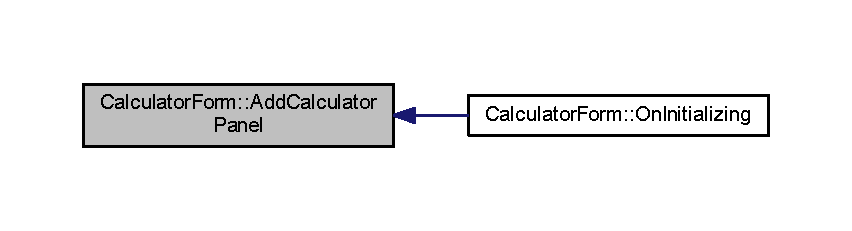
\includegraphics[width=350pt]{class_calculator_form_a52e5c1d6ce0269a59bebb3921206a7f8_icgraph}
\end{center}
\end{figure}


\hypertarget{class_calculator_form_af7bffc0f7f761c4b89fb12a8020c161e}{\index{Calculator\+Form@{Calculator\+Form}!Add\+Engineer@{Add\+Engineer}}
\index{Add\+Engineer@{Add\+Engineer}!Calculator\+Form@{Calculator\+Form}}
\subsubsection[{Add\+Engineer}]{\setlength{\rightskip}{0pt plus 5cm}void Calculator\+Form\+::\+Add\+Engineer (
\begin{DoxyParamCaption}
\item[{Tizen\+::\+Base\+::\+String}]{exp}
\end{DoxyParamCaption}
)\hspace{0.3cm}{\ttfamily [private]}}}\label{class_calculator_form_af7bffc0f7f761c4b89fb12a8020c161e}


Calculator\+Form.\+cpp 파일의 552 번째 라인에서 정의되었습니다.


\begin{DoxyCode}
552                                                     \{
553 
554     \textcolor{keywordflow}{if} (\hyperlink{_calculator_form_8cpp_afab1dc0f42edf6d2d70e1a3b9a23114b}{pNum\_Showing} > \hyperlink{_calculator_form_8cpp_abece60225b3a6a5859e110ffa820effc}{MAX\_SHOWING\_NUM}) \{
555         \hyperlink{class_calculator_form_a47822c0c78fff69b9d3ebdb8a5f9a7a4}{ShowErrorPopup}(\textcolor{stringliteral}{"수식은 150자를 넘길 수 없습니다."});
556     \} \textcolor{keywordflow}{else} \{
557         String temp = \hyperlink{class_calculator_form_a85c791f34a8b69e7d22b7d64d7f69bac}{\_\_pLabelExpression}->GetText();
558         \textcolor{keywordflow}{if} (temp == \textcolor{stringliteral}{"0"}) \{
559             \hyperlink{class_calculator_form_a85c791f34a8b69e7d22b7d64d7f69bac}{\_\_pLabelExpression}->SetText(\textcolor{stringliteral}{""});
560             \hyperlink{_calculator_form_8cpp_a8e641e0c730e6831fcb8e9caf57f5285}{pExpression} = \textcolor{stringliteral}{""};
561             \hyperlink{_calculator_form_8cpp_afab1dc0f42edf6d2d70e1a3b9a23114b}{pNum\_Showing} = 0;
562         \}
563 
564         \textcolor{keywordflow}{if} (!(\hyperlink{_calculator_form_8cpp_a710068ff7294670ef87617fd3e379c41}{pResultFlag} == \hyperlink{_calculator_form_8cpp_ae7b7d386a4346e31a05841a90ca2067d}{RESULT\_ERR})) \{
565             \hyperlink{_calculator_form_8cpp_a710068ff7294670ef87617fd3e379c41}{pResultFlag} = \hyperlink{_calculator_form_8cpp_a364808cb06bdb87add9aa111ff5ae3d4}{NO\_RESULT};
566             String pExp;
567             \textcolor{keywordtype}{int} pBefore = \hyperlink{class_calculator_form_af8fd474cf2173be9fa0dbbdfc114b5b3}{Before}(1);
568             \textcolor{comment}{//Change exp for pExpression}
569             \textcolor{keywordflow}{if} (exp == \textcolor{stringliteral}{"sin("}) \{
570                 pExp = \textcolor{stringliteral}{"s("};
571                 \hyperlink{_calculator_form_8cpp_a5a03127e257bb5f5d935e038dcf8d834}{pNum\_Paren}++;
572                 \hyperlink{_calculator_form_8cpp_afab1dc0f42edf6d2d70e1a3b9a23114b}{pNum\_Showing} += 4;
573             \} \textcolor{keywordflow}{else} \textcolor{keywordflow}{if} (exp == \textcolor{stringliteral}{"cos("}) \{
574                 pExp = \textcolor{stringliteral}{"c("};
575                 \hyperlink{_calculator_form_8cpp_a5a03127e257bb5f5d935e038dcf8d834}{pNum\_Paren}++;
576                 \hyperlink{_calculator_form_8cpp_afab1dc0f42edf6d2d70e1a3b9a23114b}{pNum\_Showing} += 4;
577             \} \textcolor{keywordflow}{else} \textcolor{keywordflow}{if} (exp == \textcolor{stringliteral}{"tan("}) \{
578                 pExp = \textcolor{stringliteral}{"t("};
579                 \hyperlink{_calculator_form_8cpp_a5a03127e257bb5f5d935e038dcf8d834}{pNum\_Paren}++;
580                 \hyperlink{_calculator_form_8cpp_afab1dc0f42edf6d2d70e1a3b9a23114b}{pNum\_Showing} += 4;
581             \} \textcolor{keywordflow}{else} \textcolor{keywordflow}{if} (exp == \textcolor{stringliteral}{"ln("}) \{
582                 pExp = \textcolor{stringliteral}{"l("};
583                 \hyperlink{_calculator_form_8cpp_a5a03127e257bb5f5d935e038dcf8d834}{pNum\_Paren}++;
584                 \hyperlink{_calculator_form_8cpp_afab1dc0f42edf6d2d70e1a3b9a23114b}{pNum\_Showing} += 4;
585             \} \textcolor{keywordflow}{else} \textcolor{keywordflow}{if} (exp == \textcolor{stringliteral}{"log("}) \{
586                 pExp = \textcolor{stringliteral}{"g("};
587                 \hyperlink{_calculator_form_8cpp_a5a03127e257bb5f5d935e038dcf8d834}{pNum\_Paren}++;
588                 \hyperlink{_calculator_form_8cpp_afab1dc0f42edf6d2d70e1a3b9a23114b}{pNum\_Showing} += 4;
589             \} \textcolor{keywordflow}{else} \textcolor{keywordflow}{if} (exp == \textcolor{stringliteral}{"abs("}) \{
590                 pExp = \textcolor{stringliteral}{"a("};
591                 \hyperlink{_calculator_form_8cpp_a5a03127e257bb5f5d935e038dcf8d834}{pNum\_Paren}++;
592                 \hyperlink{_calculator_form_8cpp_afab1dc0f42edf6d2d70e1a3b9a23114b}{pNum\_Showing} += 4;
593             \} \textcolor{keywordflow}{else} \textcolor{keywordflow}{if} (exp == \textcolor{stringliteral}{"ROOT"}) \{
594                 exp = \textcolor{stringliteral}{"√("};
595                 \hyperlink{_calculator_form_8cpp_a5a03127e257bb5f5d935e038dcf8d834}{pNum\_Paren}++;
596                 pExp = \textcolor{stringliteral}{"r("};
597                 \hyperlink{_calculator_form_8cpp_afab1dc0f42edf6d2d70e1a3b9a23114b}{pNum\_Showing} += 2;
598             \} \textcolor{keywordflow}{else} \textcolor{keywordflow}{if} (exp == \textcolor{stringliteral}{"Y^x"}) \{
599                 exp = \textcolor{stringliteral}{"^("};
600                 pExp = \textcolor{stringliteral}{"^("};
601                 \hyperlink{_calculator_form_8cpp_a5a03127e257bb5f5d935e038dcf8d834}{pNum\_Paren}++;
602                 \hyperlink{_calculator_form_8cpp_afab1dc0f42edf6d2d70e1a3b9a23114b}{pNum\_Showing} += 2;
603             \} \textcolor{keywordflow}{else} \textcolor{keywordflow}{if} (exp == \textcolor{stringliteral}{"x^2"}) \{
604                 exp = \textcolor{stringliteral}{"^(2)"};
605                 pExp = \textcolor{stringliteral}{"^(2)"};
606                 \hyperlink{_calculator_form_8cpp_afab1dc0f42edf6d2d70e1a3b9a23114b}{pNum\_Showing} += 4;
607             \} \textcolor{keywordflow}{else} \textcolor{keywordflow}{if} (exp == \textcolor{stringliteral}{"Pi"}) \{
608                 pExp = \textcolor{stringliteral}{"p"};
609                 \hyperlink{_calculator_form_8cpp_afab1dc0f42edf6d2d70e1a3b9a23114b}{pNum\_Showing} += 2;
610             \} \textcolor{keywordflow}{else} \{
611                 pExp = exp;
612             \}
613 
614             \textcolor{keywordflow}{if} (exp == \textcolor{stringliteral}{"^("} || exp == \textcolor{stringliteral}{"^(2)"} || exp == \textcolor{stringliteral}{"!"}) \{
615 
616                 \textcolor{comment}{//Means pBefore is an operand}
617                 \textcolor{keywordflow}{if} (pBefore <= \hyperlink{_calculator_form_8cpp_a310731b27bb8f16b0f5fdfeae1f7ffb5}{OPERAND\_NOT\_NUMBER}) \{
618                     \hyperlink{class_calculator_form_a85c791f34a8b69e7d22b7d64d7f69bac}{\_\_pLabelExpression}->SetText(
619                             \hyperlink{class_calculator_form_a85c791f34a8b69e7d22b7d64d7f69bac}{\_\_pLabelExpression}->GetText() + exp);
620                     \hyperlink{_calculator_form_8cpp_a8e641e0c730e6831fcb8e9caf57f5285}{pExpression} = \hyperlink{_calculator_form_8cpp_a8e641e0c730e6831fcb8e9caf57f5285}{pExpression} + pExp;
621                 \} \textcolor{keywordflow}{else} \textcolor{keywordflow}{if} (pBefore == \hyperlink{_calculator_form_8cpp_a5f2b2f460e2ebcf757c348d74ed9ef68}{DOT}) \{
622                     \hyperlink{class_calculator_form_a85c791f34a8b69e7d22b7d64d7f69bac}{\_\_pLabelExpression}->SetText(
623                             \hyperlink{class_calculator_form_a85c791f34a8b69e7d22b7d64d7f69bac}{\_\_pLabelExpression}->GetText() + \textcolor{stringliteral}{"0"} + exp);
624                     \hyperlink{_calculator_form_8cpp_a8e641e0c730e6831fcb8e9caf57f5285}{pExpression} = \hyperlink{_calculator_form_8cpp_a8e641e0c730e6831fcb8e9caf57f5285}{pExpression} + \textcolor{stringliteral}{"0"} + pExp;
625                     \hyperlink{_calculator_form_8cpp_af728e21ac3463ebc5e7746a542efb32f}{pDotFlag} = \textcolor{keyword}{false};
626                     \hyperlink{_calculator_form_8cpp_afab1dc0f42edf6d2d70e1a3b9a23114b}{pNum\_Showing}++;
627                 \} \textcolor{keywordflow}{else} \{
628                     \hyperlink{class_calculator_form_a47822c0c78fff69b9d3ebdb8a5f9a7a4}{ShowErrorPopup}(\textcolor{stringliteral}{"입력값 오류!"});
629                 \}
630             \} \textcolor{keywordflow}{else} \{
631                 \textcolor{keywordflow}{if} (exp == \textcolor{stringliteral}{"e^("} || exp == \textcolor{stringliteral}{"1/("}) \{
632                     \hyperlink{_calculator_form_8cpp_a5a03127e257bb5f5d935e038dcf8d834}{pNum\_Paren}++;
633                     \hyperlink{_calculator_form_8cpp_afab1dc0f42edf6d2d70e1a3b9a23114b}{pNum\_Showing} += 3;
634                 \} \textcolor{keywordflow}{else} \{
635                     \hyperlink{_calculator_form_8cpp_afab1dc0f42edf6d2d70e1a3b9a23114b}{pNum\_Showing}++;
636                 \}
637                 \textcolor{comment}{//Means pBefore is an operand}
638                 \textcolor{keywordflow}{if} (pBefore <= \hyperlink{_calculator_form_8cpp_a310731b27bb8f16b0f5fdfeae1f7ffb5}{OPERAND\_NOT\_NUMBER}) \{
639                     \hyperlink{class_calculator_form_a85c791f34a8b69e7d22b7d64d7f69bac}{\_\_pLabelExpression}->SetText(
640                             \hyperlink{class_calculator_form_a85c791f34a8b69e7d22b7d64d7f69bac}{\_\_pLabelExpression}->GetText() + \textcolor{stringliteral}{"*"} + exp);
641                     \hyperlink{_calculator_form_8cpp_a8e641e0c730e6831fcb8e9caf57f5285}{pExpression} = \hyperlink{_calculator_form_8cpp_a8e641e0c730e6831fcb8e9caf57f5285}{pExpression} + \textcolor{stringliteral}{"*"} + pExp;
642                     \hyperlink{_calculator_form_8cpp_afab1dc0f42edf6d2d70e1a3b9a23114b}{pNum\_Showing}++;
643                 \} \textcolor{keywordflow}{else} \textcolor{keywordflow}{if} (pBefore == \hyperlink{_calculator_form_8cpp_a5f2b2f460e2ebcf757c348d74ed9ef68}{DOT}) \{
644                     \hyperlink{class_calculator_form_a85c791f34a8b69e7d22b7d64d7f69bac}{\_\_pLabelExpression}->SetText(
645                             \hyperlink{class_calculator_form_a85c791f34a8b69e7d22b7d64d7f69bac}{\_\_pLabelExpression}->GetText() + \textcolor{stringliteral}{"0*"} + exp);
646                     \hyperlink{_calculator_form_8cpp_a8e641e0c730e6831fcb8e9caf57f5285}{pExpression} = \hyperlink{_calculator_form_8cpp_a8e641e0c730e6831fcb8e9caf57f5285}{pExpression} + \textcolor{stringliteral}{"0*"} + pExp;
647                     \hyperlink{_calculator_form_8cpp_afab1dc0f42edf6d2d70e1a3b9a23114b}{pNum\_Showing} += 2;
648                     \hyperlink{_calculator_form_8cpp_af728e21ac3463ebc5e7746a542efb32f}{pDotFlag} = \textcolor{keyword}{false};
649                 \} \textcolor{keywordflow}{else} \{
650                     \hyperlink{class_calculator_form_a85c791f34a8b69e7d22b7d64d7f69bac}{\_\_pLabelExpression}->SetText(
651                             \hyperlink{class_calculator_form_a85c791f34a8b69e7d22b7d64d7f69bac}{\_\_pLabelExpression}->GetText() + exp);
652                     \hyperlink{_calculator_form_8cpp_a8e641e0c730e6831fcb8e9caf57f5285}{pExpression} = \hyperlink{_calculator_form_8cpp_a8e641e0c730e6831fcb8e9caf57f5285}{pExpression} + pExp;
653                 \}
654 
655             \}
656             \hyperlink{_calculator_form_8cpp_a564e048fb0774fad296f0ce77b108d23}{pNum\_Operand}[0] = 0;
657             \hyperlink{_calculator_form_8cpp_a564e048fb0774fad296f0ce77b108d23}{pNum\_Operand}[1] = 0;
658             \hyperlink{class_calculator_form_ac55d87afff38e894b348eeb01a058c70}{SetLabelTextSize}();
659             AppLog(\textcolor{stringliteral}{"%d : %d"}, \hyperlink{_calculator_form_8cpp_a564e048fb0774fad296f0ce77b108d23}{pNum\_Operand}[0], \hyperlink{_calculator_form_8cpp_a564e048fb0774fad296f0ce77b108d23}{pNum\_Operand}[1]);
660         \}
661     \}
662 \}
\end{DoxyCode}


이 함수 내부에서 호출하는 함수들에 대한 그래프입니다.\+:
\nopagebreak
\begin{figure}[H]
\begin{center}
\leavevmode
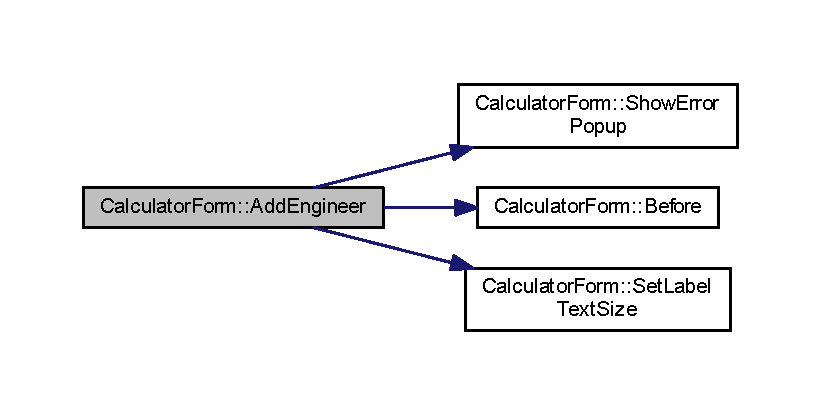
\includegraphics[width=350pt]{class_calculator_form_af7bffc0f7f761c4b89fb12a8020c161e_cgraph}
\end{center}
\end{figure}




이 함수를 호출하는 함수들에 대한 그래프입니다.\+:
\nopagebreak
\begin{figure}[H]
\begin{center}
\leavevmode
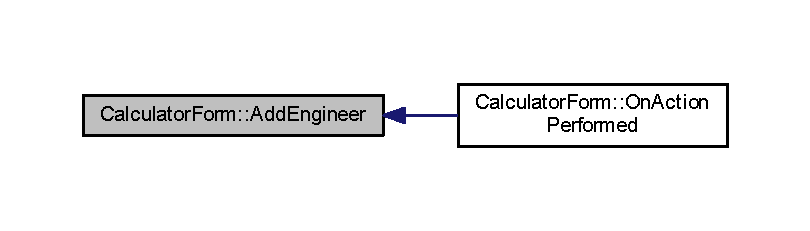
\includegraphics[width=350pt]{class_calculator_form_af7bffc0f7f761c4b89fb12a8020c161e_icgraph}
\end{center}
\end{figure}


\hypertarget{class_calculator_form_a06eb55916ba3f358cbe5502eb5f12cff}{\index{Calculator\+Form@{Calculator\+Form}!Add\+Error\+Popup@{Add\+Error\+Popup}}
\index{Add\+Error\+Popup@{Add\+Error\+Popup}!Calculator\+Form@{Calculator\+Form}}
\subsubsection[{Add\+Error\+Popup}]{\setlength{\rightskip}{0pt plus 5cm}result Calculator\+Form\+::\+Add\+Error\+Popup (
\begin{DoxyParamCaption}
\item[{void}]{}
\end{DoxyParamCaption}
)\hspace{0.3cm}{\ttfamily [private]}}}\label{class_calculator_form_a06eb55916ba3f358cbe5502eb5f12cff}


Calculator\+Form.\+cpp 파일의 250 번째 라인에서 정의되었습니다.


\begin{DoxyCode}
250                                          \{
251     result r = E\_SUCCESS;
252     Button* pBtnOK = null;
253 
254     \hyperlink{class_calculator_form_aa22a98e80f0533746ca5c712ea3b7a8e}{\_\_pPopup} = \textcolor{keyword}{new} (std::nothrow) Popup();
255     TryReturn(\hyperlink{class_calculator_form_aa22a98e80f0533746ca5c712ea3b7a8e}{\_\_pPopup} != null, E\_OUT\_OF\_MEMORY,
256             \textcolor{stringliteral}{"Unable to allocate memory for error pop-up"});
257 
258     r = \hyperlink{class_calculator_form_aa22a98e80f0533746ca5c712ea3b7a8e}{\_\_pPopup}->Construct(\textcolor{keyword}{true}, \hyperlink{_calculator_form_8cpp_a3efdfa9e0e3df2363389bb8cc1fbb4ac}{POPUP\_DIMENSION});
259     TryCatch(!IsFailed(r), \textcolor{comment}{/* NOP */},
260             \textcolor{stringliteral}{"Pop-up::Construct() with [%s]"}, GetErrorMessage(r));
261 
262     \hyperlink{class_calculator_form_aabf0dd69d2567ee96db776f4bbe53f4e}{\_\_pPopup\_Label} = \textcolor{keyword}{new} (std::nothrow) Label();
263     TryCatch(\hyperlink{class_calculator_form_aabf0dd69d2567ee96db776f4bbe53f4e}{\_\_pPopup\_Label} != null, r = E\_OUT\_OF\_MEMORY,
264     \textcolor{stringliteral}{"Unable to allocate memory for error label"});
265 
266     r = \hyperlink{class_calculator_form_aabf0dd69d2567ee96db776f4bbe53f4e}{\_\_pPopup\_Label}->Construct(\hyperlink{_calculator_form_8cpp_a71dcdf817688131706205d3b70932daa}{POPUP\_LABEL\_RECT}, L\textcolor{stringliteral}{""});
267     TryCatch(!IsFailed(r), \textcolor{keyword}{delete} \hyperlink{class_calculator_form_aabf0dd69d2567ee96db776f4bbe53f4e}{\_\_pPopup\_Label},
268             \textcolor{stringliteral}{"Label::Construct() with [%s]"}, GetErrorMessage(r));
269 
270     \hyperlink{class_calculator_form_aabf0dd69d2567ee96db776f4bbe53f4e}{\_\_pPopup\_Label}->SetText(L\textcolor{stringliteral}{""});
271 
272     r = \hyperlink{class_calculator_form_aa22a98e80f0533746ca5c712ea3b7a8e}{\_\_pPopup}->AddControl(\hyperlink{class_calculator_form_aabf0dd69d2567ee96db776f4bbe53f4e}{\_\_pPopup\_Label});
273     TryCatch(!IsFailed(r), \textcolor{keyword}{delete} \hyperlink{class_calculator_form_aabf0dd69d2567ee96db776f4bbe53f4e}{\_\_pPopup\_Label},
274             \textcolor{stringliteral}{"Pop-up::AddControl() with [%s]"}, GetErrorMessage(r));
275 
276     pBtnOK = \textcolor{keyword}{new} (std::nothrow) Button();
277     TryCatch(pBtnOK != null, r = E\_OUT\_OF\_MEMORY,
278     \textcolor{stringliteral}{"Unable to allocate memory for ok button"});
279 
280     r = pBtnOK->Construct(\hyperlink{_calculator_form_8cpp_a74c6359e95c3c71ca337eba85c026a3f}{POPUP\_BTN\_RECT}, L\textcolor{stringliteral}{"OK"});
281     TryCatch(!IsFailed(r), \textcolor{keyword}{delete} pBtnOK, \textcolor{stringliteral}{"Button::Construct() with [%s]"},
282             GetErrorMessage(r));
283 
284     pBtnOK->SetActionId(\hyperlink{_calculator_form_8cpp_aed8e9c49324ebdd0f39324bff6a882b2}{ACTION\_ID\_POPUP\_BTN\_OK});
285     pBtnOK->AddActionEventListener(*\textcolor{keyword}{this});
286 
287     \hyperlink{class_calculator_form_aa22a98e80f0533746ca5c712ea3b7a8e}{\_\_pPopup}->AddControl(pBtnOK);
288     TryCatch(!IsFailed(r), \textcolor{keyword}{delete} pBtnOK, \textcolor{stringliteral}{"Pop-up::AddControl() with [%s]"},
289             GetErrorMessage(r));
290 
291     \textcolor{keywordflow}{return} E\_SUCCESS;
292 
293     CATCH: \textcolor{keyword}{delete} \hyperlink{class_calculator_form_aa22a98e80f0533746ca5c712ea3b7a8e}{\_\_pPopup};
294     \hyperlink{class_calculator_form_aa22a98e80f0533746ca5c712ea3b7a8e}{\_\_pPopup} = null;
295     \textcolor{keywordflow}{return} r;
296 \}
\end{DoxyCode}


이 함수 내부에서 호출하는 함수들에 대한 그래프입니다.\+:
\nopagebreak
\begin{figure}[H]
\begin{center}
\leavevmode
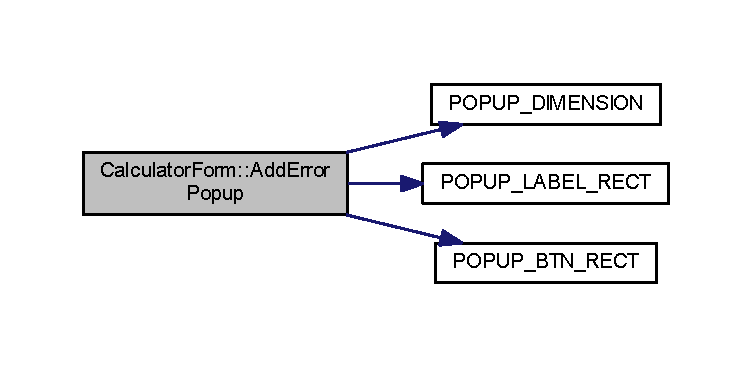
\includegraphics[width=350pt]{class_calculator_form_a06eb55916ba3f358cbe5502eb5f12cff_cgraph}
\end{center}
\end{figure}




이 함수를 호출하는 함수들에 대한 그래프입니다.\+:
\nopagebreak
\begin{figure}[H]
\begin{center}
\leavevmode
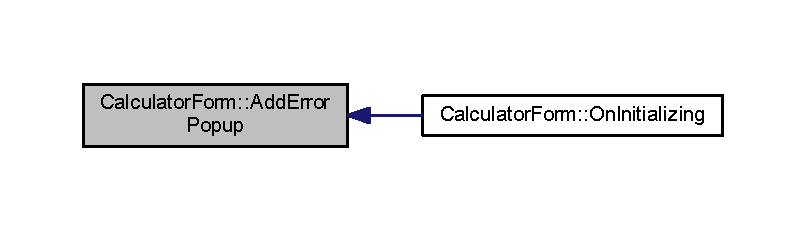
\includegraphics[width=350pt]{class_calculator_form_a06eb55916ba3f358cbe5502eb5f12cff_icgraph}
\end{center}
\end{figure}


\hypertarget{class_calculator_form_ab703941d3327dc7ec09c377427786ecd}{\index{Calculator\+Form@{Calculator\+Form}!Add\+List\+\_\+\+Init@{Add\+List\+\_\+\+Init}}
\index{Add\+List\+\_\+\+Init@{Add\+List\+\_\+\+Init}!Calculator\+Form@{Calculator\+Form}}
\subsubsection[{Add\+List\+\_\+\+Init}]{\setlength{\rightskip}{0pt plus 5cm}result Calculator\+Form\+::\+Add\+List\+\_\+\+Init (
\begin{DoxyParamCaption}
\item[{void}]{}
\end{DoxyParamCaption}
)\hspace{0.3cm}{\ttfamily [private]}}}\label{class_calculator_form_ab703941d3327dc7ec09c377427786ecd}


Calculator\+Form.\+cpp 파일의 136 번째 라인에서 정의되었습니다.


\begin{DoxyCode}
136                                         \{
137 
138     \hyperlink{class_calculator_form_abb49d4c96119ee3adaf6a9bf8302ddaa}{\_\_sensorMgr}.Construct();
139 
140     \hyperlink{class_calculator_form_a7b784d40a3d83eee41bb8efae09142ca}{Rawtiltpitch}.Construct();
141     \hyperlink{class_calculator_form_afc8797d0cb7657a384ccc03c7f335aed}{Rawtiltroll}.Construct();
142 
143     \hyperlink{class_calculator_form_a63438d1ef5396e2d216eaf604659c96c}{Filteredtiltroll}.Construct();
144     \hyperlink{class_calculator_form_a54065fa7531b14c744c8d11ccd849f81}{Filteredtiltpitch}.Construct();
145 
146     result r = E\_SUCCESS;
147     \textcolor{keywordflow}{return} r;
148 \}
\end{DoxyCode}


이 함수를 호출하는 함수들에 대한 그래프입니다.\+:
\nopagebreak
\begin{figure}[H]
\begin{center}
\leavevmode
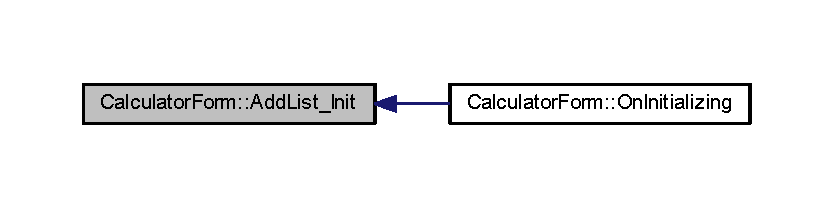
\includegraphics[width=350pt]{class_calculator_form_ab703941d3327dc7ec09c377427786ecd_icgraph}
\end{center}
\end{figure}


\hypertarget{class_calculator_form_ad23e66a668778e9354b831dbac18a689}{\index{Calculator\+Form@{Calculator\+Form}!Add\+Operand@{Add\+Operand}}
\index{Add\+Operand@{Add\+Operand}!Calculator\+Form@{Calculator\+Form}}
\subsubsection[{Add\+Operand}]{\setlength{\rightskip}{0pt plus 5cm}void Calculator\+Form\+::\+Add\+Operand (
\begin{DoxyParamCaption}
\item[{Tizen\+::\+Base\+::\+String}]{exp}
\end{DoxyParamCaption}
)\hspace{0.3cm}{\ttfamily [private]}}}\label{class_calculator_form_ad23e66a668778e9354b831dbac18a689}


Calculator\+Form.\+cpp 파일의 443 번째 라인에서 정의되었습니다.


\begin{DoxyCode}
443                                                    \{
444     \textcolor{keywordflow}{if} (\hyperlink{_calculator_form_8cpp_afab1dc0f42edf6d2d70e1a3b9a23114b}{pNum\_Showing} > \hyperlink{_calculator_form_8cpp_abece60225b3a6a5859e110ffa820effc}{MAX\_SHOWING\_NUM}) \{
445         \hyperlink{class_calculator_form_a47822c0c78fff69b9d3ebdb8a5f9a7a4}{ShowErrorPopup}(\textcolor{stringliteral}{"수식은 150자를 넘길 수 없습니다."});
446     \} \textcolor{keywordflow}{else} \{
447         \textcolor{keywordflow}{if} (\hyperlink{_calculator_form_8cpp_a564e048fb0774fad296f0ce77b108d23}{pNum\_Operand}[0] > \hyperlink{_calculator_form_8cpp_a1258c84a63ca70eeae6059a9eeb74b30}{MAX\_OPERANDS}) \{
448             \hyperlink{class_calculator_form_a47822c0c78fff69b9d3ebdb8a5f9a7a4}{ShowErrorPopup}(\textcolor{stringliteral}{"숫자는 16자를 넘길 수 없습니다."});
449         \} \textcolor{keywordflow}{else} \textcolor{keywordflow}{if} (\hyperlink{_calculator_form_8cpp_a564e048fb0774fad296f0ce77b108d23}{pNum\_Operand}[1] > \hyperlink{_calculator_form_8cpp_a86ae0b330fe83154bcbb21288d26418e}{MAX\_UNDER\_DOT}) \{
450             \hyperlink{class_calculator_form_a47822c0c78fff69b9d3ebdb8a5f9a7a4}{ShowErrorPopup}(\textcolor{stringliteral}{"소숫점 이하 10자리 수를 넘길 수 없습니다."});
451         \} \textcolor{keywordflow}{else} \{
452 
453             \textcolor{keywordflow}{if} (\hyperlink{_calculator_form_8cpp_a710068ff7294670ef87617fd3e379c41}{pResultFlag} == \hyperlink{_calculator_form_8cpp_ad415544fff20c80892fa7e5555722776}{RESULT\_OK} || \hyperlink{_calculator_form_8cpp_a710068ff7294670ef87617fd3e379c41}{pResultFlag} == 
      \hyperlink{_calculator_form_8cpp_ae7b7d386a4346e31a05841a90ca2067d}{RESULT\_ERR}) \{
454                 \hyperlink{_calculator_form_8cpp_a8e641e0c730e6831fcb8e9caf57f5285}{pExpression} = \textcolor{stringliteral}{""};
455                 \hyperlink{class_calculator_form_a85c791f34a8b69e7d22b7d64d7f69bac}{\_\_pLabelExpression}->SetText(\textcolor{stringliteral}{""});
456                 \hyperlink{_calculator_form_8cpp_a710068ff7294670ef87617fd3e379c41}{pResultFlag} = \hyperlink{_calculator_form_8cpp_a364808cb06bdb87add9aa111ff5ae3d4}{NO\_RESULT};
457             \}
458             \textcolor{keywordtype}{int} pBefore = \hyperlink{class_calculator_form_af8fd474cf2173be9fa0dbbdfc114b5b3}{Before}(1);
459             \textcolor{comment}{// Handle 0 to 9}
460             \textcolor{keywordflow}{switch} (pBefore) \{
461             \textcolor{keywordflow}{case} \hyperlink{_calculator_form_8cpp_ace8ca5226379bd4e27e83a4fa65b4730}{OPERAND\_NUMBER\_0}: \{
462                 \textcolor{keywordtype}{int} pDoubleBefore = \hyperlink{class_calculator_form_af8fd474cf2173be9fa0dbbdfc114b5b3}{Before}(2);
463                 \textcolor{keywordflow}{if} (pDoubleBefore > \hyperlink{_calculator_form_8cpp_a1f5ddbd63e4020c3e1ab02f2a8a272ea}{OPERAND\_NUMBER\_NOT\_0}) \{
464                     \hyperlink{_calculator_form_8cpp_a8e641e0c730e6831fcb8e9caf57f5285}{pExpression}.Remove(\hyperlink{_calculator_form_8cpp_a8e641e0c730e6831fcb8e9caf57f5285}{pExpression}.GetLength() - 1, 1);
465                     \hyperlink{_calculator_form_8cpp_a8e641e0c730e6831fcb8e9caf57f5285}{pExpression} = \hyperlink{_calculator_form_8cpp_a8e641e0c730e6831fcb8e9caf57f5285}{pExpression} + exp;
466 
467                     String pBackExp = \hyperlink{class_calculator_form_a85c791f34a8b69e7d22b7d64d7f69bac}{\_\_pLabelExpression}->GetText();
468                     pBackExp.Remove(pBackExp.GetLength() - 1, 1);
469                     \hyperlink{class_calculator_form_a85c791f34a8b69e7d22b7d64d7f69bac}{\_\_pLabelExpression}->SetText(pBackExp + exp);
470                     \hyperlink{_calculator_form_8cpp_afab1dc0f42edf6d2d70e1a3b9a23114b}{pNum\_Showing}--;
471                     \hyperlink{_calculator_form_8cpp_a564e048fb0774fad296f0ce77b108d23}{pNum\_Operand}[0]--;
472                 \} \textcolor{keywordflow}{else} \{
473                     \hyperlink{class_calculator_form_a85c791f34a8b69e7d22b7d64d7f69bac}{\_\_pLabelExpression}->SetText(
474                             \hyperlink{class_calculator_form_a85c791f34a8b69e7d22b7d64d7f69bac}{\_\_pLabelExpression}->GetText() + exp);
475                     \hyperlink{_calculator_form_8cpp_a8e641e0c730e6831fcb8e9caf57f5285}{pExpression} = \hyperlink{_calculator_form_8cpp_a8e641e0c730e6831fcb8e9caf57f5285}{pExpression} + exp;
476                 \}
477                 \textcolor{keywordflow}{break};
478             \}
479             \textcolor{keywordflow}{case} \hyperlink{_calculator_form_8cpp_a310731b27bb8f16b0f5fdfeae1f7ffb5}{OPERAND\_NOT\_NUMBER}: \{
480                 \hyperlink{class_calculator_form_a85c791f34a8b69e7d22b7d64d7f69bac}{\_\_pLabelExpression}->SetText(
481                         \hyperlink{class_calculator_form_a85c791f34a8b69e7d22b7d64d7f69bac}{\_\_pLabelExpression}->GetText() + \textcolor{stringliteral}{"*"} + exp);
482                 \hyperlink{_calculator_form_8cpp_a8e641e0c730e6831fcb8e9caf57f5285}{pExpression} = \hyperlink{_calculator_form_8cpp_a8e641e0c730e6831fcb8e9caf57f5285}{pExpression} + \textcolor{stringliteral}{"*"} + exp;
483                 \hyperlink{_calculator_form_8cpp_afab1dc0f42edf6d2d70e1a3b9a23114b}{pNum\_Showing}++;
484                 \textcolor{keywordflow}{break};
485             \}
486             \textcolor{keywordflow}{default}: \{
487                 \hyperlink{class_calculator_form_a85c791f34a8b69e7d22b7d64d7f69bac}{\_\_pLabelExpression}->SetText(
488                         \hyperlink{class_calculator_form_a85c791f34a8b69e7d22b7d64d7f69bac}{\_\_pLabelExpression}->GetText() + exp);
489                 \hyperlink{_calculator_form_8cpp_a8e641e0c730e6831fcb8e9caf57f5285}{pExpression} = \hyperlink{_calculator_form_8cpp_a8e641e0c730e6831fcb8e9caf57f5285}{pExpression} + exp;
490                 \textcolor{keywordflow}{break};
491             \}
492             \}
493 
494             \hyperlink{_calculator_form_8cpp_a564e048fb0774fad296f0ce77b108d23}{pNum\_Operand}[0]++;
495             \textcolor{keywordflow}{if} (\hyperlink{_calculator_form_8cpp_af728e21ac3463ebc5e7746a542efb32f}{pDotFlag})
496                 \hyperlink{_calculator_form_8cpp_a564e048fb0774fad296f0ce77b108d23}{pNum\_Operand}[1]++;
497 
498             \hyperlink{_calculator_form_8cpp_afab1dc0f42edf6d2d70e1a3b9a23114b}{pNum\_Showing}++;
499             \hyperlink{class_calculator_form_ac55d87afff38e894b348eeb01a058c70}{SetLabelTextSize}();
500         \}
501     \}
502 \}
\end{DoxyCode}


이 함수 내부에서 호출하는 함수들에 대한 그래프입니다.\+:
\nopagebreak
\begin{figure}[H]
\begin{center}
\leavevmode
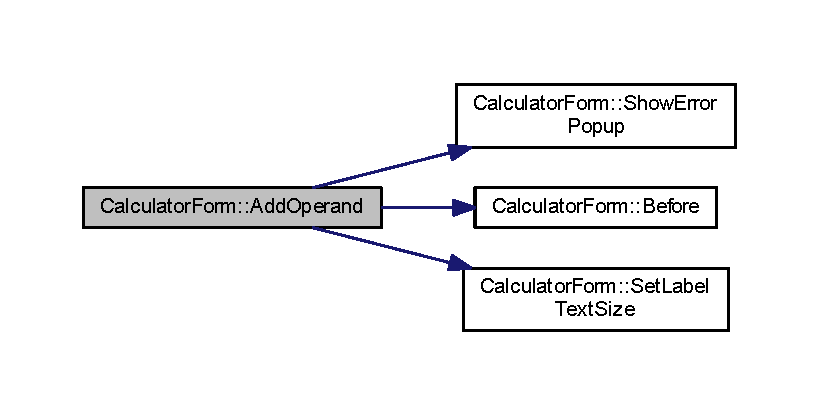
\includegraphics[width=350pt]{class_calculator_form_ad23e66a668778e9354b831dbac18a689_cgraph}
\end{center}
\end{figure}




이 함수를 호출하는 함수들에 대한 그래프입니다.\+:
\nopagebreak
\begin{figure}[H]
\begin{center}
\leavevmode
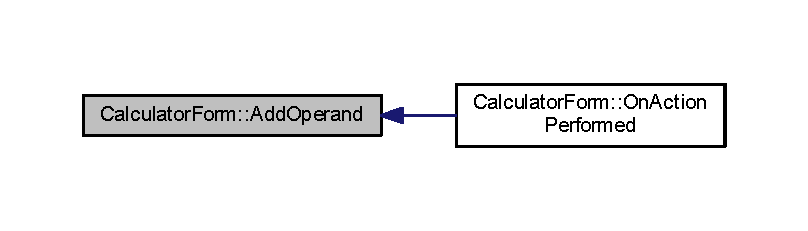
\includegraphics[width=350pt]{class_calculator_form_ad23e66a668778e9354b831dbac18a689_icgraph}
\end{center}
\end{figure}


\hypertarget{class_calculator_form_a5c68963771fb4527131e84d4963d7c14}{\index{Calculator\+Form@{Calculator\+Form}!Add\+Operator@{Add\+Operator}}
\index{Add\+Operator@{Add\+Operator}!Calculator\+Form@{Calculator\+Form}}
\subsubsection[{Add\+Operator}]{\setlength{\rightskip}{0pt plus 5cm}void Calculator\+Form\+::\+Add\+Operator (
\begin{DoxyParamCaption}
\item[{Tizen\+::\+Base\+::\+String}]{exp}
\end{DoxyParamCaption}
)\hspace{0.3cm}{\ttfamily [private]}}}\label{class_calculator_form_a5c68963771fb4527131e84d4963d7c14}


Calculator\+Form.\+cpp 파일의 504 번째 라인에서 정의되었습니다.


\begin{DoxyCode}
504                                                     \{
505     \textcolor{keywordflow}{if} (\hyperlink{_calculator_form_8cpp_afab1dc0f42edf6d2d70e1a3b9a23114b}{pNum\_Showing} > \hyperlink{_calculator_form_8cpp_abece60225b3a6a5859e110ffa820effc}{MAX\_SHOWING\_NUM}) \{
506         \hyperlink{class_calculator_form_a47822c0c78fff69b9d3ebdb8a5f9a7a4}{ShowErrorPopup}(\textcolor{stringliteral}{"수식은 150자를 넘길 수 없습니다."});
507     \} \textcolor{keywordflow}{else} \{
508         \textcolor{keywordflow}{if} (!(\hyperlink{_calculator_form_8cpp_a710068ff7294670ef87617fd3e379c41}{pResultFlag} == \hyperlink{_calculator_form_8cpp_ae7b7d386a4346e31a05841a90ca2067d}{RESULT\_ERR})) \{
509             \hyperlink{_calculator_form_8cpp_a710068ff7294670ef87617fd3e379c41}{pResultFlag} = \hyperlink{_calculator_form_8cpp_a364808cb06bdb87add9aa111ff5ae3d4}{NO\_RESULT};
510             \textcolor{keywordtype}{int} pBefore = \hyperlink{class_calculator_form_af8fd474cf2173be9fa0dbbdfc114b5b3}{Before}(1);
511 
512             \textcolor{keywordflow}{switch} (pBefore) \{
513             \textcolor{keywordflow}{case} \hyperlink{_calculator_form_8cpp_a197d8d1c652619a50380202a7c4c722c}{OPERATOR}: \{
514 
515                 \hyperlink{_calculator_form_8cpp_a8e641e0c730e6831fcb8e9caf57f5285}{pExpression}.Remove(\hyperlink{_calculator_form_8cpp_a8e641e0c730e6831fcb8e9caf57f5285}{pExpression}.GetLength() - 1, 1);
516                 \hyperlink{_calculator_form_8cpp_a8e641e0c730e6831fcb8e9caf57f5285}{pExpression} = \hyperlink{_calculator_form_8cpp_a8e641e0c730e6831fcb8e9caf57f5285}{pExpression} + exp;
517 
518                 String pBackExp = \hyperlink{class_calculator_form_a85c791f34a8b69e7d22b7d64d7f69bac}{\_\_pLabelExpression}->GetText();
519                 pBackExp.Remove(pBackExp.GetLength() - 1, 1);
520                 \hyperlink{class_calculator_form_a85c791f34a8b69e7d22b7d64d7f69bac}{\_\_pLabelExpression}->SetText(pBackExp + exp);
521                 \hyperlink{_calculator_form_8cpp_afab1dc0f42edf6d2d70e1a3b9a23114b}{pNum\_Showing}--;
522                 \textcolor{keywordflow}{break};
523             \}
524             \textcolor{keywordflow}{case} \hyperlink{_calculator_form_8cpp_a5f2b2f460e2ebcf757c348d74ed9ef68}{DOT}: \{
525                 \hyperlink{class_calculator_form_a85c791f34a8b69e7d22b7d64d7f69bac}{\_\_pLabelExpression}->SetText(
526                         \hyperlink{class_calculator_form_a85c791f34a8b69e7d22b7d64d7f69bac}{\_\_pLabelExpression}->GetText() + \textcolor{stringliteral}{"0"} + exp);
527                 \hyperlink{_calculator_form_8cpp_a8e641e0c730e6831fcb8e9caf57f5285}{pExpression} = \hyperlink{_calculator_form_8cpp_a8e641e0c730e6831fcb8e9caf57f5285}{pExpression} + \textcolor{stringliteral}{"0"} + exp;
528                 \hyperlink{_calculator_form_8cpp_afab1dc0f42edf6d2d70e1a3b9a23114b}{pNum\_Showing}++;
529                 \textcolor{keywordflow}{break};
530             \}
531             \textcolor{keywordflow}{case} \hyperlink{_calculator_form_8cpp_a2e2495cea3bd7d632d8e9f822cca5398}{LEFT\_PAREN}:
532             \textcolor{keywordflow}{case} \hyperlink{_calculator_form_8cpp_a7b20f1b443e093d5ec5e990e73b47232}{NONE}:
533                 \textcolor{keywordflow}{break};
534             \textcolor{keywordflow}{default}: \{
535                 \hyperlink{class_calculator_form_a85c791f34a8b69e7d22b7d64d7f69bac}{\_\_pLabelExpression}->SetText(
536                         \hyperlink{class_calculator_form_a85c791f34a8b69e7d22b7d64d7f69bac}{\_\_pLabelExpression}->GetText() + exp);
537                 \hyperlink{_calculator_form_8cpp_a8e641e0c730e6831fcb8e9caf57f5285}{pExpression} = \hyperlink{_calculator_form_8cpp_a8e641e0c730e6831fcb8e9caf57f5285}{pExpression} + exp;
538                 \textcolor{keywordflow}{break};
539             \}
540             \}
541 
542             \hyperlink{_calculator_form_8cpp_a564e048fb0774fad296f0ce77b108d23}{pNum\_Operand}[0] = 0;
543             \hyperlink{_calculator_form_8cpp_a564e048fb0774fad296f0ce77b108d23}{pNum\_Operand}[1] = 0;
544             \hyperlink{_calculator_form_8cpp_af728e21ac3463ebc5e7746a542efb32f}{pDotFlag} = \textcolor{keyword}{false};
545             \hyperlink{class_calculator_form_ac55d87afff38e894b348eeb01a058c70}{SetLabelTextSize}();
546             AppLog(\textcolor{stringliteral}{"%d : %d"}, \hyperlink{_calculator_form_8cpp_a564e048fb0774fad296f0ce77b108d23}{pNum\_Operand}[0], \hyperlink{_calculator_form_8cpp_a564e048fb0774fad296f0ce77b108d23}{pNum\_Operand}[1]);
547             \hyperlink{_calculator_form_8cpp_afab1dc0f42edf6d2d70e1a3b9a23114b}{pNum\_Showing}++;
548         \}
549     \}
550 \}
\end{DoxyCode}


이 함수 내부에서 호출하는 함수들에 대한 그래프입니다.\+:
\nopagebreak
\begin{figure}[H]
\begin{center}
\leavevmode
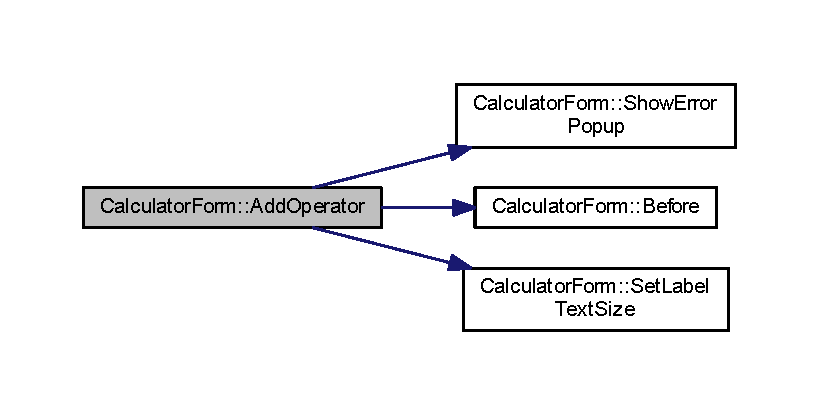
\includegraphics[width=350pt]{class_calculator_form_a5c68963771fb4527131e84d4963d7c14_cgraph}
\end{center}
\end{figure}




이 함수를 호출하는 함수들에 대한 그래프입니다.\+:
\nopagebreak
\begin{figure}[H]
\begin{center}
\leavevmode
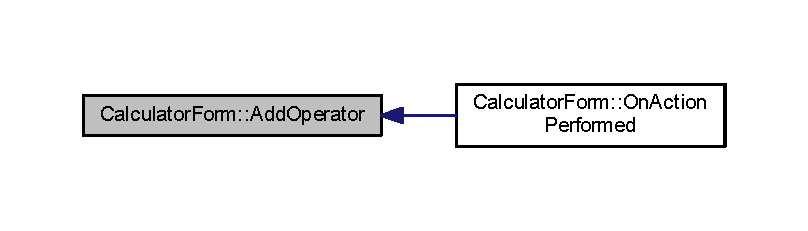
\includegraphics[width=350pt]{class_calculator_form_a5c68963771fb4527131e84d4963d7c14_icgraph}
\end{center}
\end{figure}


\hypertarget{class_calculator_form_af8fd474cf2173be9fa0dbbdfc114b5b3}{\index{Calculator\+Form@{Calculator\+Form}!Before@{Before}}
\index{Before@{Before}!Calculator\+Form@{Calculator\+Form}}
\subsubsection[{Before}]{\setlength{\rightskip}{0pt plus 5cm}int Calculator\+Form\+::\+Before (
\begin{DoxyParamCaption}
\item[{int}]{index}
\end{DoxyParamCaption}
)\hspace{0.3cm}{\ttfamily [private]}}}\label{class_calculator_form_af8fd474cf2173be9fa0dbbdfc114b5b3}


Calculator\+Form.\+cpp 파일의 966 번째 라인에서 정의되었습니다.


\begin{DoxyCode}
966                                     \{
967     \textcolor{keywordtype}{int} result = 0;
968 
969     \textcolor{keywordflow}{if} (\hyperlink{_calculator_form_8cpp_a8e641e0c730e6831fcb8e9caf57f5285}{pExpression}.GetLength() < index) \{
970         result = \hyperlink{_calculator_form_8cpp_a7b20f1b443e093d5ec5e990e73b47232}{NONE};
971     \} \textcolor{keywordflow}{else} \{
972         \textcolor{keywordtype}{wchar\_t} temp;
973         \hyperlink{_calculator_form_8cpp_a8e641e0c730e6831fcb8e9caf57f5285}{pExpression}.GetCharAt(\hyperlink{_calculator_form_8cpp_a8e641e0c730e6831fcb8e9caf57f5285}{pExpression}.GetLength() - index, temp);
974 
975         \textcolor{keywordflow}{if} (temp > \textcolor{charliteral}{'0'} && temp <= \textcolor{charliteral}{'9'}) \{
976             result = \hyperlink{_calculator_form_8cpp_a1f5ddbd63e4020c3e1ab02f2a8a272ea}{OPERAND\_NUMBER\_NOT\_0};
977         \} \textcolor{keywordflow}{else} \textcolor{keywordflow}{if} (temp == \textcolor{charliteral}{'0'}) \{
978             result = \hyperlink{_calculator_form_8cpp_ace8ca5226379bd4e27e83a4fa65b4730}{OPERAND\_NUMBER\_0};
979         \} \textcolor{keywordflow}{else} \textcolor{keywordflow}{if} (temp == \textcolor{charliteral}{'!'} || temp == \textcolor{charliteral}{')'} || temp == \textcolor{charliteral}{'e'} || temp == \textcolor{charliteral}{'p'}) \{
980             result = \hyperlink{_calculator_form_8cpp_a310731b27bb8f16b0f5fdfeae1f7ffb5}{OPERAND\_NOT\_NUMBER};
981         \} \textcolor{keywordflow}{else} \textcolor{keywordflow}{if} (temp == \textcolor{charliteral}{'.'}) \{
982             result = \hyperlink{_calculator_form_8cpp_a5f2b2f460e2ebcf757c348d74ed9ef68}{DOT};
983         \} \textcolor{keywordflow}{else} \textcolor{keywordflow}{if} (temp == \textcolor{charliteral}{'+'} || temp == \textcolor{charliteral}{'-'} || temp == \textcolor{charliteral}{'/'} || temp == \textcolor{charliteral}{'*'}
984                 || temp == \textcolor{charliteral}{'%'}) \{
985             result = \hyperlink{_calculator_form_8cpp_a197d8d1c652619a50380202a7c4c722c}{OPERATOR};
986         \} \textcolor{keywordflow}{else} \textcolor{keywordflow}{if} (temp == \textcolor{charliteral}{'('}) \{
987             result = \hyperlink{_calculator_form_8cpp_a2e2495cea3bd7d632d8e9f822cca5398}{LEFT\_PAREN};
988         \} \textcolor{keywordflow}{else} \{
989             result = \hyperlink{_calculator_form_8cpp_aa6eb89cee0001804b9de052a34777c2e}{ETC};
990         \}
991     \}
992 
993     \textcolor{keywordflow}{return} result;
994 \}
\end{DoxyCode}


이 함수를 호출하는 함수들에 대한 그래프입니다.\+:
\nopagebreak
\begin{figure}[H]
\begin{center}
\leavevmode
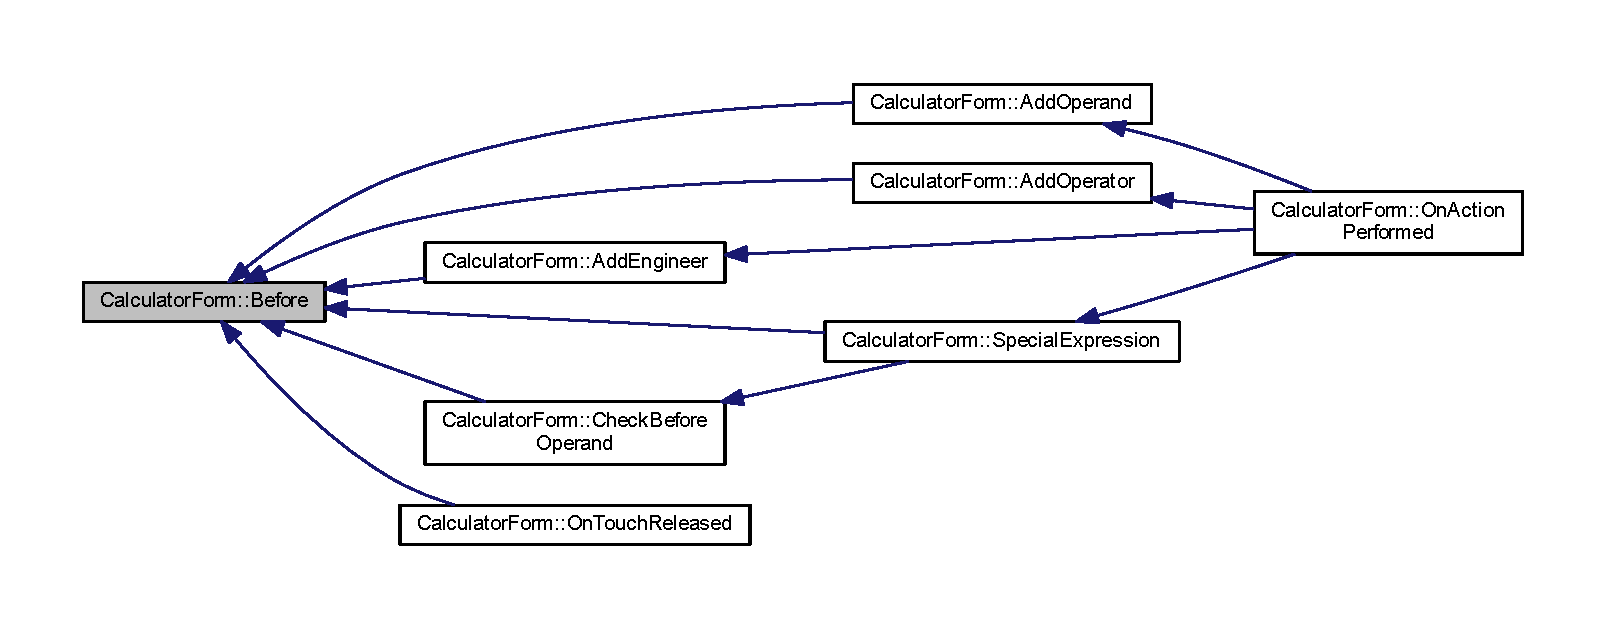
\includegraphics[width=350pt]{class_calculator_form_af8fd474cf2173be9fa0dbbdfc114b5b3_icgraph}
\end{center}
\end{figure}


\hypertarget{class_calculator_form_ac322abae9350aee54dba283e68c94d5d}{\index{Calculator\+Form@{Calculator\+Form}!Check\+Before\+Operand@{Check\+Before\+Operand}}
\index{Check\+Before\+Operand@{Check\+Before\+Operand}!Calculator\+Form@{Calculator\+Form}}
\subsubsection[{Check\+Before\+Operand}]{\setlength{\rightskip}{0pt plus 5cm}int $\ast$ Calculator\+Form\+::\+Check\+Before\+Operand (
\begin{DoxyParamCaption}
\item[{Tizen\+::\+Base\+::\+String}]{expression}
\end{DoxyParamCaption}
)\hspace{0.3cm}{\ttfamily [private]}}}\label{class_calculator_form_ac322abae9350aee54dba283e68c94d5d}


Calculator\+Form.\+cpp 파일의 996 번째 라인에서 정의되었습니다.


\begin{DoxyCode}
996                                                                   \{
997     \textcolor{keywordtype}{int}* pResult = \textcolor{keyword}{new} \textcolor{keywordtype}{int}[2];
998     \textcolor{keywordtype}{int} current = 0;
999     \textcolor{keywordtype}{wchar\_t} temp;
1000 
1001     \textcolor{keywordflow}{if} (expression.GetLength() == 1) \{
1002         pResult[0] = \hyperlink{_calculator_form_8cpp_a4fc4627e993b733f1716e4f657fed196}{ADD\_SIGN\_EMPTY};
1003         pResult[1] = 0;
1004         AppLog(\textcolor{stringliteral}{"ADD\_SIGN\_EMPTY"});
1005         \textcolor{keywordflow}{return} pResult;
1006     \}
1007 
1008     \textcolor{keywordflow}{for} (\textcolor{keywordtype}{int} i = 1; i < expression.GetLength() + 2; i++) \{
1009         current = \hyperlink{class_calculator_form_af8fd474cf2173be9fa0dbbdfc114b5b3}{Before}(i);
1010 
1011         \textcolor{keywordflow}{if} (current == \hyperlink{_calculator_form_8cpp_a197d8d1c652619a50380202a7c4c722c}{OPERATOR}) \{
1012             expression.GetCharAt(expression.GetLength() - i, temp);
1013             \textcolor{keywordflow}{if} (temp == \textcolor{charliteral}{'+'} || temp == \textcolor{charliteral}{'/'} || temp == \textcolor{charliteral}{'*'} || temp == \textcolor{charliteral}{'('}
1014                     || temp == \textcolor{charliteral}{'%'}) \{
1015                 pResult[0] = \hyperlink{_calculator_form_8cpp_aa80a5225e90cdfa081a9d871229028cd}{ADD\_SIGN\_ETC};
1016                 pResult[1] = i;
1017                 \textcolor{keywordflow}{break};
1018 
1019             \} \textcolor{keywordflow}{else} \textcolor{keywordflow}{if} (temp == \textcolor{charliteral}{'-'}) \{
1020                 expression.GetCharAt(expression.GetLength() - (i + 1), temp);
1021                 \textcolor{keywordflow}{if} (temp == \textcolor{charliteral}{'('}) \{
1022                     pResult[0] = \hyperlink{_calculator_form_8cpp_a454db45292332cab043f74d3acefa482}{DELETE\_SIGN};
1023                     pResult[1] = i;
1024                     \textcolor{keywordflow}{break};
1025                 \} \textcolor{keywordflow}{else} \{
1026                     pResult[0] = \hyperlink{_calculator_form_8cpp_ab34236baa7c9cb7ea0b2c833a27683da}{ADD\_SIGN\_MINUS};
1027                     pResult[1] = i;
1028                     \textcolor{keywordflow}{break};
1029                 \}
1030             \}
1031         \} \textcolor{keywordflow}{else} \textcolor{keywordflow}{if} (current == \hyperlink{_calculator_form_8cpp_a2e2495cea3bd7d632d8e9f822cca5398}{LEFT\_PAREN}) \{
1032             pResult[0] = \hyperlink{_calculator_form_8cpp_aa80a5225e90cdfa081a9d871229028cd}{ADD\_SIGN\_ETC};
1033             pResult[1] = i;
1034             \textcolor{keywordflow}{break};
1035         \} \textcolor{keywordflow}{else} \textcolor{keywordflow}{if} (current == \hyperlink{_calculator_form_8cpp_a7b20f1b443e093d5ec5e990e73b47232}{NONE}) \{
1036             pResult[0] = \hyperlink{_calculator_form_8cpp_aeb4c35ea92719283cfd04e4d553d35f9}{ADD\_SIGN\_START};
1037             pResult[1] = i;
1038             \textcolor{keywordflow}{break};
1039         \}
1040     \}
1041     \textcolor{keywordflow}{return} pResult;
1042 \}
\end{DoxyCode}


이 함수 내부에서 호출하는 함수들에 대한 그래프입니다.\+:
\nopagebreak
\begin{figure}[H]
\begin{center}
\leavevmode
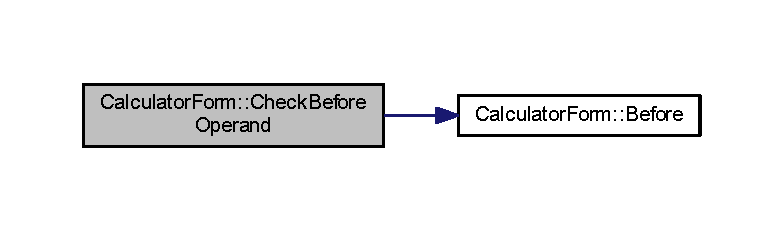
\includegraphics[width=350pt]{class_calculator_form_ac322abae9350aee54dba283e68c94d5d_cgraph}
\end{center}
\end{figure}




이 함수를 호출하는 함수들에 대한 그래프입니다.\+:
\nopagebreak
\begin{figure}[H]
\begin{center}
\leavevmode
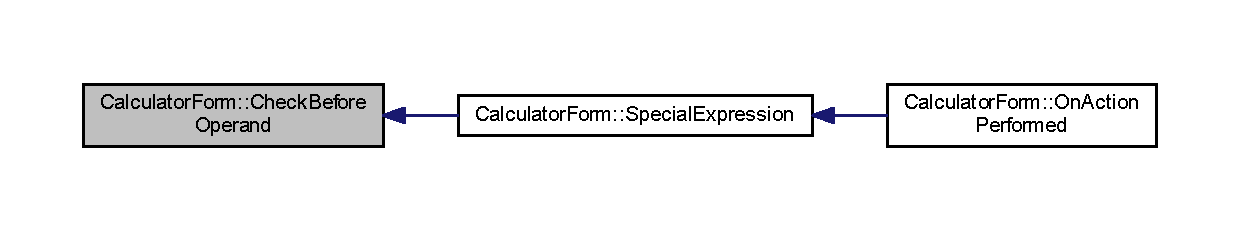
\includegraphics[width=350pt]{class_calculator_form_ac322abae9350aee54dba283e68c94d5d_icgraph}
\end{center}
\end{figure}


\hypertarget{class_calculator_form_a3c0dcddf79a19546615f51c2acf989a9}{\index{Calculator\+Form@{Calculator\+Form}!clear\+Buffer@{clear\+Buffer}}
\index{clear\+Buffer@{clear\+Buffer}!Calculator\+Form@{Calculator\+Form}}
\subsubsection[{clear\+Buffer}]{\setlength{\rightskip}{0pt plus 5cm}void Calculator\+Form\+::clear\+Buffer (
\begin{DoxyParamCaption}
\item[{void}]{}
\end{DoxyParamCaption}
)\hspace{0.3cm}{\ttfamily [private]}}}\label{class_calculator_form_a3c0dcddf79a19546615f51c2acf989a9}


Calculator\+Form.\+cpp 파일의 1235 번째 라인에서 정의되었습니다.


\begin{DoxyCode}
1235                                  \{
1236     AppLog(\textcolor{stringliteral}{"Clear Buffer..."});
1237 
1238     \hyperlink{class_calculator_form_afc8797d0cb7657a384ccc03c7f335aed}{Rawtiltroll}.RemoveAll();
1239     \hyperlink{class_calculator_form_a7b784d40a3d83eee41bb8efae09142ca}{Rawtiltpitch}.RemoveAll();
1240 
1241     \hyperlink{class_calculator_form_a54065fa7531b14c744c8d11ccd849f81}{Filteredtiltpitch}.RemoveAll();
1242     \hyperlink{class_calculator_form_a63438d1ef5396e2d216eaf604659c96c}{Filteredtiltroll}.RemoveAll();
1243 
1244 \}
\end{DoxyCode}


이 함수를 호출하는 함수들에 대한 그래프입니다.\+:
\nopagebreak
\begin{figure}[H]
\begin{center}
\leavevmode
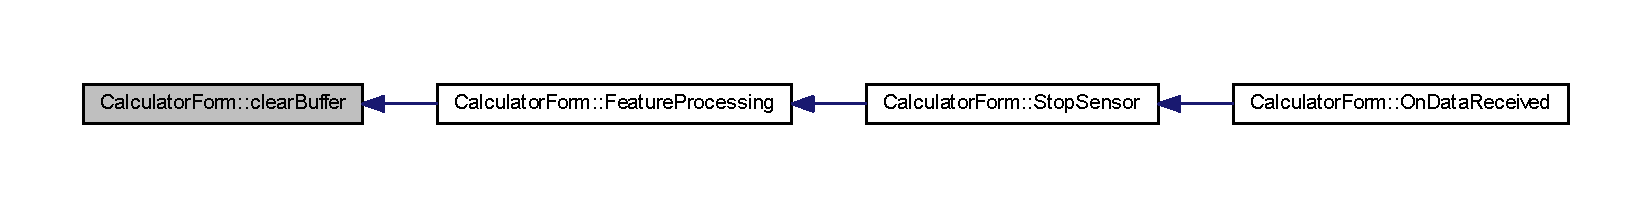
\includegraphics[width=350pt]{class_calculator_form_a3c0dcddf79a19546615f51c2acf989a9_icgraph}
\end{center}
\end{figure}


\hypertarget{class_calculator_form_ae739bb0f8aea14c0ae2d440950130bc2}{\index{Calculator\+Form@{Calculator\+Form}!Feature\+Processing@{Feature\+Processing}}
\index{Feature\+Processing@{Feature\+Processing}!Calculator\+Form@{Calculator\+Form}}
\subsubsection[{Feature\+Processing}]{\setlength{\rightskip}{0pt plus 5cm}void Calculator\+Form\+::\+Feature\+Processing (
\begin{DoxyParamCaption}
\item[{void}]{}
\end{DoxyParamCaption}
)}}\label{class_calculator_form_ae739bb0f8aea14c0ae2d440950130bc2}


Calculator\+Form.\+cpp 파일의 1246 번째 라인에서 정의되었습니다.


\begin{DoxyCode}
1246                                        \{
1247 
1248     std::vector<std::string> input;
1249 
1250     \textcolor{keywordtype}{double} *result\_label = \textcolor{keyword}{new} \textcolor{keywordtype}{double}[3];
1251     \textcolor{keywordtype}{int} *retVal = \textcolor{keyword}{new} \textcolor{keywordtype}{int}[3];
1252 
1253     retVal[0]=0;
1254     retVal[1]=0;
1255     retVal[2]=0;
1256 
1257     \textcolor{keywordtype}{int} cast\_label = 0;
1258     \textcolor{keywordtype}{float} mean\_pitch, mean\_roll;
1259 
1260     \textcolor{keywordtype}{int} port = 0;
1261     \textcolor{keywordtype}{int} land = 1;
1262     \textcolor{keywordtype}{int} reverse = 2;
1263     \textcolor{keywordtype}{int} orientation = 0;
1264 
1265     String label\_history;
1266 
1267     \textcolor{comment}{//Orientation 을 Feature 1로 추가하는 부분}
1268     OrientationStatus status = GetOrientationStatus();
1269 
1270     \textcolor{comment}{//portrait = 0, land = 1, reverse = 2}
1271     \textcolor{keywordflow}{if} (status == ORIENTATION\_STATUS\_PORTRAIT
1272             || status == ORIENTATION\_STATUS\_PORTRAIT\_REVERSE) \{
1273         orientation = port;
1274     \} \textcolor{keywordflow}{else} \textcolor{keywordflow}{if} (status == ORIENTATION\_STATUS\_LANDSCAPE) \{
1275         orientation = land;
1276     \} \textcolor{keywordflow}{else} \{
1277         orientation = reverse;
1278     \}
1279 
1280     \hyperlink{class_calculator_form_a7219388d7692193e44e149d822035231}{lowPass}(\hyperlink{class_calculator_form_a7b784d40a3d83eee41bb8efae09142ca}{Rawtiltpitch}, \hyperlink{class_calculator_form_a54065fa7531b14c744c8d11ccd849f81}{Filteredtiltpitch});
1281     \hyperlink{class_calculator_form_a7219388d7692193e44e149d822035231}{lowPass}(\hyperlink{class_calculator_form_afc8797d0cb7657a384ccc03c7f335aed}{Rawtiltroll}, \hyperlink{class_calculator_form_a63438d1ef5396e2d216eaf604659c96c}{Filteredtiltroll});
1282 
1283     \textcolor{keywordflow}{for} (\textcolor{keywordtype}{int} i = 0; i < 3; i++) \{
1284 
1285         mean\_pitch = \hyperlink{class_calculator_form_a832965e97b000380703993d2c61e357a}{getMean}(\hyperlink{class_calculator_form_a54065fa7531b14c744c8d11ccd849f81}{Filteredtiltpitch});
1286         mean\_roll = \hyperlink{class_calculator_form_a832965e97b000380703993d2c61e357a}{getMean}(\hyperlink{class_calculator_form_a63438d1ef5396e2d216eaf604659c96c}{Filteredtiltroll});
1287 
1288         std::string inputstr = \hyperlink{_calculator_form_8cpp_a89016affff07b7f39247021035532b50}{string\_format}(\textcolor{stringliteral}{"1 1:%d 2:%f 3:%f"}, orientation,
1289                 mean\_pitch, mean\_roll);
1290         input.push\_back(inputstr);
1291 
1292         result\_label[i] = \hyperlink{class_calculator_form_ac3e3da16eada2566553b992a8d254366}{svm}.\hyperlink{class_svm_wrapper_a2f3adec2bc81b6c37416156465485e9c}{predict}(input, \hyperlink{_calculator_form_8cpp_ab961cf377425a7b81fd62afffd8e89e1}{nullfunc});
1293         cast\_label = \textcolor{keyword}{static\_cast<}\textcolor{keywordtype}{int}\textcolor{keyword}{>}(result\_label[i]);
1294         retVal[cast\_label]++;
1295         AppLog(\textcolor{stringliteral}{"retVal Count %d, %d, %d"}, retVal[0], retVal[1], retVal[2]);
1296         input.clear();
1297         \textcolor{comment}{//일단 history에 맞게 뜨는지 확인 후 최다빈출로 대표값 선정하는거 추가}
1298     \}
1299     \hyperlink{class_calculator_form_a3c0dcddf79a19546615f51c2acf989a9}{clearBuffer}();
1300 
1301     \textcolor{comment}{//가장 많이 관측된 값을 구하는 과정}
1302     \textcolor{keywordtype}{int} \hyperlink{svm_8cpp_a348440c5435269ac7c60d2e2d8916f48}{min}=-1, maxIndex=0;
1303     \textcolor{keywordflow}{for}(\textcolor{keywordtype}{int} i=0;i<3;i++)
1304     \{
1305         \textcolor{keywordflow}{if}(retVal[i]>min)
1306         \{
1307             min = retVal[i];
1308             maxIndex = i;
1309         \}
1310     \}
1311 
1312     SceneManager* pSceneManager = SceneManager::GetInstance();
1313     AppAssert(pSceneManager);
1314 
1315     \textcolor{keywordflow}{switch}(maxIndex)
1316     \{
1317     \textcolor{keywordflow}{case} \hyperlink{_calculator_form_8cpp_a9a8b3c0366194868e0e8654c8177ecf5}{TILTSTOP}:
1318         \textcolor{keywordflow}{break};
1319     \textcolor{keywordflow}{case} \hyperlink{_calculator_form_8cpp_aa1b5081998052b52a05c212786c5de75}{TILTLEFT}:
1320         pSceneManager->GoForward(ForwardSceneTransition(
      \hyperlink{_scene_register_8h_ad2cc89ed96c8bd4c94f954f01ef0f56e}{SCENE\_FILEBROWSER\_MANAGEMENT}));
1321         \textcolor{keywordflow}{break};
1322     \textcolor{keywordflow}{case} \hyperlink{_calculator_form_8cpp_a923abea421f18f4d617bae7a5ce69991}{TILTRIGHT}:
1323         pSceneManager->GoForward(ForwardSceneTransition(\hyperlink{_scene_register_8h_a941a02ceb430e35a99e905974dd4faf3}{SCENE\_FILEBROWSER\_HIDDEN}));
1324         \textcolor{keywordflow}{break};
1325     \}
1326 
1327     \textcolor{keyword}{delete}(result\_label);
1328     \textcolor{keyword}{delete}(retVal);
1329 
1330 \}
\end{DoxyCode}


이 함수 내부에서 호출하는 함수들에 대한 그래프입니다.\+:
\nopagebreak
\begin{figure}[H]
\begin{center}
\leavevmode
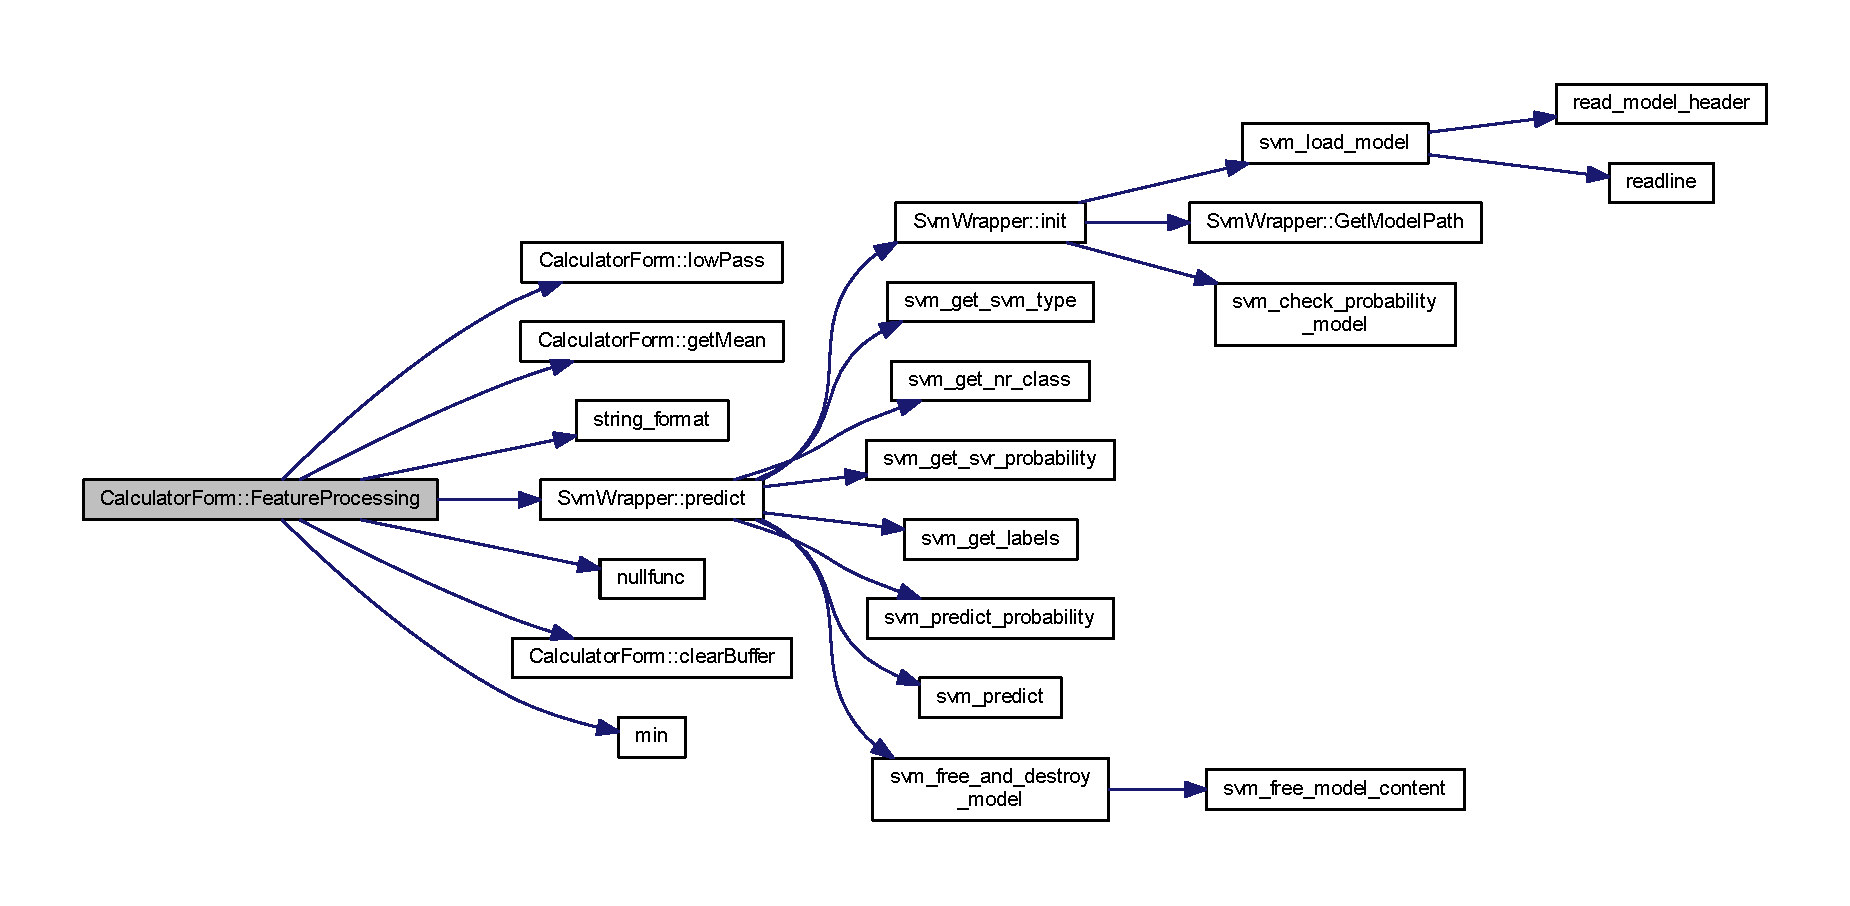
\includegraphics[width=350pt]{class_calculator_form_ae739bb0f8aea14c0ae2d440950130bc2_cgraph}
\end{center}
\end{figure}




이 함수를 호출하는 함수들에 대한 그래프입니다.\+:
\nopagebreak
\begin{figure}[H]
\begin{center}
\leavevmode
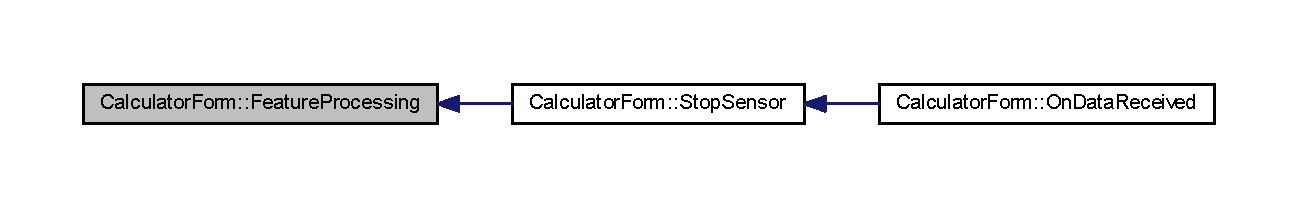
\includegraphics[width=350pt]{class_calculator_form_ae739bb0f8aea14c0ae2d440950130bc2_icgraph}
\end{center}
\end{figure}


\hypertarget{class_calculator_form_a832965e97b000380703993d2c61e357a}{\index{Calculator\+Form@{Calculator\+Form}!get\+Mean@{get\+Mean}}
\index{get\+Mean@{get\+Mean}!Calculator\+Form@{Calculator\+Form}}
\subsubsection[{get\+Mean}]{\setlength{\rightskip}{0pt plus 5cm}float Calculator\+Form\+::get\+Mean (
\begin{DoxyParamCaption}
\item[{Tizen\+::\+Base\+::\+Collection\+::\+Array\+List\+T$<$ float $>$ \&}]{param}
\end{DoxyParamCaption}
)\hspace{0.3cm}{\ttfamily [private]}}}\label{class_calculator_form_a832965e97b000380703993d2c61e357a}


Calculator\+Form.\+cpp 파일의 1215 번째 라인에서 정의되었습니다.


\begin{DoxyCode}
1216                                                      \{
1217     \textcolor{keywordtype}{float} total = 0;
1218     \textcolor{keywordtype}{float} temp = 0;
1219 
1220     \textcolor{keywordflow}{for} (\textcolor{keywordtype}{int} i = 0; i < \hyperlink{_calculator_form_8cpp_ab8328f60e764077c3155976384c62598}{SAMPLE\_WINDOWSIZE}; i++) \{
1221         \hyperlink{structsvm__model_a95f43f398a173e63d0ce26911d0a9273}{param}.GetAt(0, temp);
1222         \hyperlink{structsvm__model_a95f43f398a173e63d0ce26911d0a9273}{param}.RemoveAt(0);
1223         \textcolor{comment}{//하나씩 지우면서 처음꺼만 계속 뺌}
1224         total += temp;
1225     \}
1226 
1227     AppLog(\textcolor{stringliteral}{"OK getMean"});
1228     \textcolor{keywordflow}{return} total / (float) SAMPLE\_WINDOWSIZE;
1229 \}
\end{DoxyCode}


이 함수를 호출하는 함수들에 대한 그래프입니다.\+:
\nopagebreak
\begin{figure}[H]
\begin{center}
\leavevmode
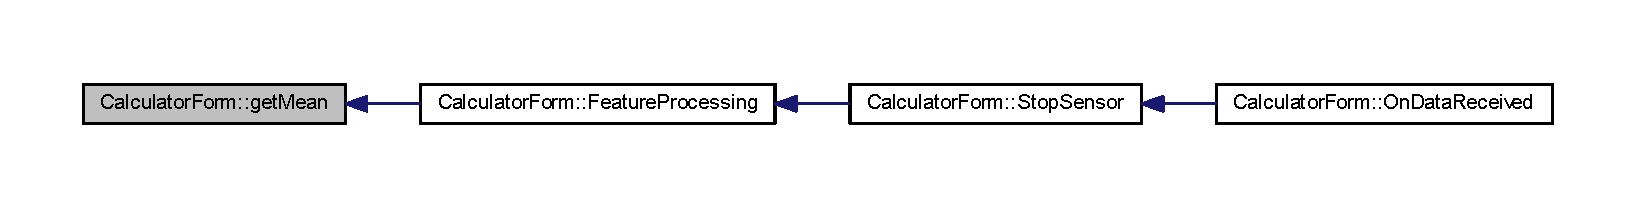
\includegraphics[width=350pt]{class_calculator_form_a832965e97b000380703993d2c61e357a_icgraph}
\end{center}
\end{figure}


\hypertarget{class_calculator_form_a51137823626f92e48605c6d9aa2e220f}{\index{Calculator\+Form@{Calculator\+Form}!Initialize@{Initialize}}
\index{Initialize@{Initialize}!Calculator\+Form@{Calculator\+Form}}
\subsubsection[{Initialize}]{\setlength{\rightskip}{0pt plus 5cm}bool Calculator\+Form\+::\+Initialize (
\begin{DoxyParamCaption}
\item[{void}]{}
\end{DoxyParamCaption}
)}}\label{class_calculator_form_a51137823626f92e48605c6d9aa2e220f}


Calculator\+Form.\+cpp 파일의 88 번째 라인에서 정의되었습니다.


\begin{DoxyCode}
88                                 \{
89     result r = Construct(\hyperlink{_app_resource_id_8h_a6ec83393c4538db99e54431ef91334f4}{IDF\_CALCULATOR\_FORM});
90     TryReturn(r == E\_SUCCESS, \textcolor{keyword}{false}, \textcolor{stringliteral}{"Failed to construct form"});
91 
92     OrientationStatus status = GetOrientationStatus();
93     \textcolor{keywordflow}{if} (status == ORIENTATION\_STATUS\_PORTRAIT
94             || status == ORIENTATION\_STATUS\_PORTRAIT\_REVERSE) \{
95         \hyperlink{class_calculator_form_a4b8ee8d07acfddbe9140a17a37b23109}{\_\_panelId} = 0;
96     \} \textcolor{keywordflow}{else} \{
97         \hyperlink{class_calculator_form_a4b8ee8d07acfddbe9140a17a37b23109}{\_\_panelId} = 1;
98     \}
99     \textcolor{keywordflow}{return} \textcolor{keyword}{true};
100 \}
\end{DoxyCode}


이 함수를 호출하는 함수들에 대한 그래프입니다.\+:
\nopagebreak
\begin{figure}[H]
\begin{center}
\leavevmode
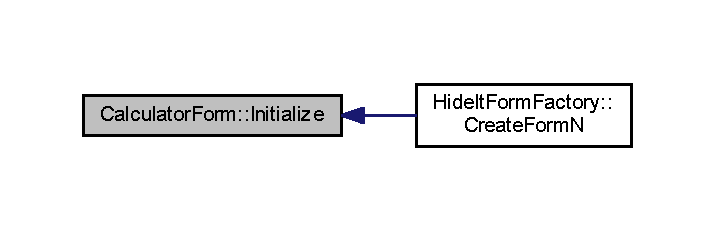
\includegraphics[width=343pt]{class_calculator_form_a51137823626f92e48605c6d9aa2e220f_icgraph}
\end{center}
\end{figure}


\hypertarget{class_calculator_form_a7219388d7692193e44e149d822035231}{\index{Calculator\+Form@{Calculator\+Form}!low\+Pass@{low\+Pass}}
\index{low\+Pass@{low\+Pass}!Calculator\+Form@{Calculator\+Form}}
\subsubsection[{low\+Pass}]{\setlength{\rightskip}{0pt plus 5cm}void Calculator\+Form\+::low\+Pass (
\begin{DoxyParamCaption}
\item[{const Tizen\+::\+Base\+::\+Collection\+::\+Array\+List\+T$<$ float $>$ \&}]{param, }
\item[{Tizen\+::\+Base\+::\+Collection\+::\+Array\+List\+T$<$ float $>$ \&}]{output}
\end{DoxyParamCaption}
)\hspace{0.3cm}{\ttfamily [private]}}}\label{class_calculator_form_a7219388d7692193e44e149d822035231}


Calculator\+Form.\+cpp 파일의 1194 번째 라인에서 정의되었습니다.


\begin{DoxyCode}
1196                                                       \{
1197     \textcolor{keywordtype}{float} raw = 1;
1198     \textcolor{keywordtype}{float} last = 0;
1199     \textcolor{keywordtype}{float} filter = 0;
1200 
1201 \textcolor{comment}{//앞에 구린 데이터를 처리하지 않도록}
1202     \hyperlink{structsvm__model_a95f43f398a173e63d0ce26911d0a9273}{param}.GetAt(0, raw);
1203     output.Add(raw);
1204 
1205     \textcolor{keywordflow}{for} (\textcolor{keywordtype}{int} i = 1; i < \hyperlink{structsvm__model_a95f43f398a173e63d0ce26911d0a9273}{param}.GetCount(); i++) \{
1206         \textcolor{comment}{//currrent data}
1207         \hyperlink{structsvm__model_a95f43f398a173e63d0ce26911d0a9273}{param}.GetAt(i, raw);
1208         output.GetAt(i - 1, last);
1209         filter = last * (1.0f - \hyperlink{_calculator_form_8cpp_a6e36f77342e4ad6a98212d3ba1f857ed}{LOWPASSWEIGHT}) + raw * 
      \hyperlink{_calculator_form_8cpp_a6e36f77342e4ad6a98212d3ba1f857ed}{LOWPASSWEIGHT};
1210         output.Add(filter);
1211     \}
1212     AppLog(\textcolor{stringliteral}{"OK lowPass"});
1213 \}
\end{DoxyCode}


이 함수를 호출하는 함수들에 대한 그래프입니다.\+:
\nopagebreak
\begin{figure}[H]
\begin{center}
\leavevmode
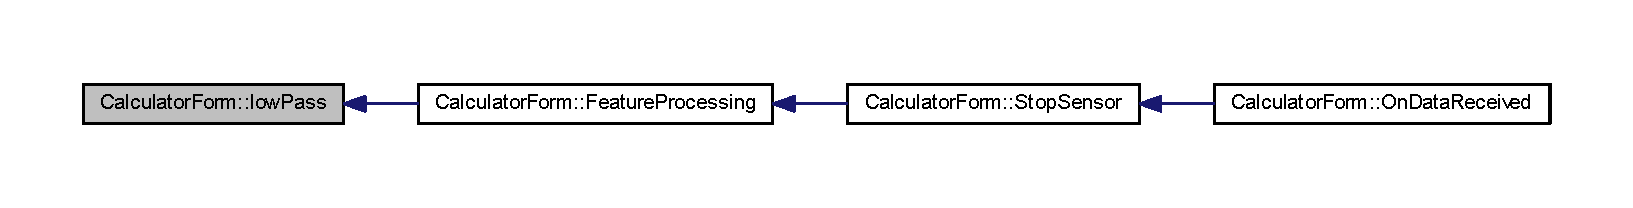
\includegraphics[width=350pt]{class_calculator_form_a7219388d7692193e44e149d822035231_icgraph}
\end{center}
\end{figure}


\hypertarget{class_calculator_form_a861aa95341240a0d98db563acc753bca}{\index{Calculator\+Form@{Calculator\+Form}!Narrow\+String@{Narrow\+String}}
\index{Narrow\+String@{Narrow\+String}!Calculator\+Form@{Calculator\+Form}}
\subsubsection[{Narrow\+String}]{\setlength{\rightskip}{0pt plus 5cm}std\+::string Calculator\+Form\+::\+Narrow\+String (
\begin{DoxyParamCaption}
\item[{const std\+::wstring \&}]{str, }
\item[{const char $\ast$}]{locale\+Name = {\ttfamily \char`\"{}C\char`\"{}}}
\end{DoxyParamCaption}
)\hspace{0.3cm}{\ttfamily [private]}}}\label{class_calculator_form_a861aa95341240a0d98db563acc753bca}
\hypertarget{class_calculator_form_af30252093893f4cb4d5578e919d3381f}{\index{Calculator\+Form@{Calculator\+Form}!On\+Action\+Performed@{On\+Action\+Performed}}
\index{On\+Action\+Performed@{On\+Action\+Performed}!Calculator\+Form@{Calculator\+Form}}
\subsubsection[{On\+Action\+Performed}]{\setlength{\rightskip}{0pt plus 5cm}void Calculator\+Form\+::\+On\+Action\+Performed (
\begin{DoxyParamCaption}
\item[{const Tizen\+::\+Ui\+::\+Control \&}]{source, }
\item[{int}]{action\+Id}
\end{DoxyParamCaption}
)\hspace{0.3cm}{\ttfamily [virtual]}}}\label{class_calculator_form_af30252093893f4cb4d5578e919d3381f}


Calculator\+Form.\+cpp 파일의 307 번째 라인에서 정의되었습니다.


\begin{DoxyCode}
308                       \{
309 
310     \textcolor{keywordflow}{switch} (actionId) \{
311     \textcolor{keywordflow}{case} \hyperlink{class_calculator_form_a7f0486405077c1eaee1faa73e631a67fa36847135c8b46dba3738ae1fdb7e3706}{ID\_NOR\_BTN\_0}:
312     \textcolor{keywordflow}{case} \hyperlink{class_calculator_form_a7f0486405077c1eaee1faa73e631a67fada58ff2bcae312b4d937de88c5e6392d}{ID\_ENG\_BTN\_0}:
313         \hyperlink{class_calculator_form_ad23e66a668778e9354b831dbac18a689}{AddOperand}(\textcolor{stringliteral}{"0"});
314         \textcolor{keywordflow}{break};
315     \textcolor{keywordflow}{case} \hyperlink{class_calculator_form_a7f0486405077c1eaee1faa73e631a67facb654bf70d6d1c0f2ba3a51e7f54bcec}{ID\_NOR\_BTN\_1}:
316     \textcolor{keywordflow}{case} \hyperlink{class_calculator_form_a7f0486405077c1eaee1faa73e631a67faa2fca2ce7488b16e9ab0154485af5474}{ID\_ENG\_BTN\_1}:
317         \hyperlink{class_calculator_form_ad23e66a668778e9354b831dbac18a689}{AddOperand}(\textcolor{stringliteral}{"1"});
318         \textcolor{keywordflow}{break};
319     \textcolor{keywordflow}{case} \hyperlink{class_calculator_form_a7f0486405077c1eaee1faa73e631a67fa5979614c050c3bcb0b3ac03c81cfbd71}{ID\_NOR\_BTN\_2}:
320     \textcolor{keywordflow}{case} \hyperlink{class_calculator_form_a7f0486405077c1eaee1faa73e631a67fa04f038704039c1943995dedb16a1dec2}{ID\_ENG\_BTN\_2}:
321         \hyperlink{class_calculator_form_ad23e66a668778e9354b831dbac18a689}{AddOperand}(\textcolor{stringliteral}{"2"});
322         \textcolor{keywordflow}{break};
323     \textcolor{keywordflow}{case} \hyperlink{class_calculator_form_a7f0486405077c1eaee1faa73e631a67fa276bf31b6dff33ed4cbb573b2f821cdb}{ID\_NOR\_BTN\_3}:
324     \textcolor{keywordflow}{case} \hyperlink{class_calculator_form_a7f0486405077c1eaee1faa73e631a67fa9dbb058cd33957c0e3f3432515a59f5f}{ID\_ENG\_BTN\_3}:
325         \hyperlink{class_calculator_form_ad23e66a668778e9354b831dbac18a689}{AddOperand}(\textcolor{stringliteral}{"3"});
326         \textcolor{keywordflow}{break};
327     \textcolor{keywordflow}{case} \hyperlink{class_calculator_form_a7f0486405077c1eaee1faa73e631a67fa74bce332df52efead67e481025bd68e6}{ID\_NOR\_BTN\_4}:
328     \textcolor{keywordflow}{case} \hyperlink{class_calculator_form_a7f0486405077c1eaee1faa73e631a67facaa578f61ab27a654264de100a480254}{ID\_ENG\_BTN\_4}:
329         \hyperlink{class_calculator_form_ad23e66a668778e9354b831dbac18a689}{AddOperand}(\textcolor{stringliteral}{"4"});
330         \textcolor{keywordflow}{break};
331     \textcolor{keywordflow}{case} \hyperlink{class_calculator_form_a7f0486405077c1eaee1faa73e631a67fa6a71324302629d7b14f8aa6a69b18ecc}{ID\_NOR\_BTN\_5}:
332     \textcolor{keywordflow}{case} \hyperlink{class_calculator_form_a7f0486405077c1eaee1faa73e631a67fa02fb238b0c78356f31d71f4028c2a966}{ID\_ENG\_BTN\_5}:
333         \hyperlink{class_calculator_form_ad23e66a668778e9354b831dbac18a689}{AddOperand}(\textcolor{stringliteral}{"5"});
334         \textcolor{keywordflow}{break};
335     \textcolor{keywordflow}{case} \hyperlink{class_calculator_form_a7f0486405077c1eaee1faa73e631a67fa6645c0b47b7414fbaf95efcdab161c83}{ID\_NOR\_BTN\_6}:
336     \textcolor{keywordflow}{case} \hyperlink{class_calculator_form_a7f0486405077c1eaee1faa73e631a67fa437b9321c7aa469549ed4c3a2d0a44d4}{ID\_ENG\_BTN\_6}:
337         \hyperlink{class_calculator_form_ad23e66a668778e9354b831dbac18a689}{AddOperand}(\textcolor{stringliteral}{"6"});
338         \textcolor{keywordflow}{break};
339     \textcolor{keywordflow}{case} \hyperlink{class_calculator_form_a7f0486405077c1eaee1faa73e631a67fa079f3395882ff05ebdab30a802a948af}{ID\_NOR\_BTN\_7}:
340     \textcolor{keywordflow}{case} \hyperlink{class_calculator_form_a7f0486405077c1eaee1faa73e631a67fa1ce33b8c2b0834d0b3c611b2a0be81d4}{ID\_ENG\_BTN\_7}:
341         \hyperlink{class_calculator_form_ad23e66a668778e9354b831dbac18a689}{AddOperand}(\textcolor{stringliteral}{"7"});
342         \textcolor{keywordflow}{break};
343     \textcolor{keywordflow}{case} \hyperlink{class_calculator_form_a7f0486405077c1eaee1faa73e631a67fa94f50ff40314d7f9580755252fefe510}{ID\_NOR\_BTN\_8}:
344     \textcolor{keywordflow}{case} \hyperlink{class_calculator_form_a7f0486405077c1eaee1faa73e631a67fa3b47082c5d91658d924c744f2aa718a5}{ID\_ENG\_BTN\_8}:
345         \hyperlink{class_calculator_form_ad23e66a668778e9354b831dbac18a689}{AddOperand}(\textcolor{stringliteral}{"8"});
346         \textcolor{keywordflow}{break};
347     \textcolor{keywordflow}{case} \hyperlink{class_calculator_form_a7f0486405077c1eaee1faa73e631a67fa0a4fbbd355bdae0d35fbc895aa177ced}{ID\_NOR\_BTN\_9}:
348     \textcolor{keywordflow}{case} \hyperlink{class_calculator_form_a7f0486405077c1eaee1faa73e631a67fa8d9bbd7046fa548f53cf7d5637804082}{ID\_ENG\_BTN\_9}:
349         \hyperlink{class_calculator_form_ad23e66a668778e9354b831dbac18a689}{AddOperand}(\textcolor{stringliteral}{"9"});
350         \textcolor{keywordflow}{break};
351     \textcolor{keywordflow}{case} \hyperlink{class_calculator_form_a7f0486405077c1eaee1faa73e631a67fa399bc7ab7ecdeb3e2160376c94e59b6a}{ID\_NOR\_BTN\_MINUS}:
352     \textcolor{keywordflow}{case} \hyperlink{class_calculator_form_a7f0486405077c1eaee1faa73e631a67fa0b2145bcc8d621a0813d82172311ce3f}{ID\_ENG\_BTN\_MINUS}:
353         \hyperlink{class_calculator_form_a5c68963771fb4527131e84d4963d7c14}{AddOperator}(\textcolor{stringliteral}{"-"});
354         \textcolor{keywordflow}{break};
355     \textcolor{keywordflow}{case} \hyperlink{class_calculator_form_a7f0486405077c1eaee1faa73e631a67faa5b58117f4dd98124b55dd697ab2bb5a}{ID\_NOR\_BTN\_PLUS}:
356     \textcolor{keywordflow}{case} \hyperlink{class_calculator_form_a7f0486405077c1eaee1faa73e631a67fa7e49dbbe01a555e1cdc467a31d6646c5}{ID\_ENG\_BTN\_PLUS}:
357         \hyperlink{class_calculator_form_a5c68963771fb4527131e84d4963d7c14}{AddOperator}(\textcolor{stringliteral}{"+"});
358         \textcolor{keywordflow}{break};
359     \textcolor{keywordflow}{case} \hyperlink{class_calculator_form_a7f0486405077c1eaee1faa73e631a67fabac2fde992d2d7d97ffcbd7f21352d4c}{ID\_NOR\_BTN\_MULTIPLY}:
360     \textcolor{keywordflow}{case} \hyperlink{class_calculator_form_a7f0486405077c1eaee1faa73e631a67face617b5a3f58f07423eea9111b63132e}{ID\_ENG\_BTN\_MULTIPLY}:
361         \hyperlink{class_calculator_form_a5c68963771fb4527131e84d4963d7c14}{AddOperator}(\textcolor{stringliteral}{"*"});
362         \textcolor{keywordflow}{break};
363     \textcolor{keywordflow}{case} \hyperlink{class_calculator_form_a7f0486405077c1eaee1faa73e631a67fac05e591891daa63c36e391a458b012b2}{ID\_NOR\_BTN\_DIVIDE}:
364     \textcolor{keywordflow}{case} \hyperlink{class_calculator_form_a7f0486405077c1eaee1faa73e631a67fa23fcaaf8e46bd3ee549352e7233af15e}{ID\_ENG\_BTN\_DIVIDE}:
365         \hyperlink{class_calculator_form_a5c68963771fb4527131e84d4963d7c14}{AddOperator}(\textcolor{stringliteral}{"/"});
366         \textcolor{keywordflow}{break};
367     \textcolor{keywordflow}{case} \hyperlink{class_calculator_form_a7f0486405077c1eaee1faa73e631a67fabf47eac7bede8b3614af465f83944d25}{ID\_ENG\_BTN\_FACTO}:
368         \hyperlink{class_calculator_form_af7bffc0f7f761c4b89fb12a8020c161e}{AddEngineer}(\textcolor{stringliteral}{"!"});
369         \textcolor{keywordflow}{break};
370     \textcolor{keywordflow}{case} \hyperlink{class_calculator_form_a7f0486405077c1eaee1faa73e631a67fafafc4a31d9c1a9d5333f09bf852bbe3f}{ID\_ENG\_BTN\_PERCENT}:
371         \hyperlink{class_calculator_form_a5c68963771fb4527131e84d4963d7c14}{AddOperator}(\textcolor{stringliteral}{"%"});
372         \textcolor{keywordflow}{break};
373     \textcolor{keywordflow}{case} \hyperlink{class_calculator_form_a7f0486405077c1eaee1faa73e631a67faa0899f6f1819e97246d4a2e7d638b14c}{ID\_ENG\_BTN\_SIN}:
374         \hyperlink{class_calculator_form_af7bffc0f7f761c4b89fb12a8020c161e}{AddEngineer}(\textcolor{stringliteral}{"sin("});
375         \textcolor{keywordflow}{break};
376     \textcolor{keywordflow}{case} \hyperlink{class_calculator_form_a7f0486405077c1eaee1faa73e631a67faa0fb52e70f50596259fecf8e0ce037f5}{ID\_ENG\_BTN\_COS}:
377         \hyperlink{class_calculator_form_af7bffc0f7f761c4b89fb12a8020c161e}{AddEngineer}(\textcolor{stringliteral}{"cos("});
378         \textcolor{keywordflow}{break};
379     \textcolor{keywordflow}{case} \hyperlink{class_calculator_form_a7f0486405077c1eaee1faa73e631a67faf99e3f69403a41412e639c269fcc87d3}{ID\_ENG\_BTN\_TAN}:
380         \hyperlink{class_calculator_form_af7bffc0f7f761c4b89fb12a8020c161e}{AddEngineer}(\textcolor{stringliteral}{"tan("});
381         \textcolor{keywordflow}{break};
382     \textcolor{keywordflow}{case} \hyperlink{class_calculator_form_a7f0486405077c1eaee1faa73e631a67fa72adc19c50013f5027bcccf22006d5d0}{ID\_ENG\_BTN\_LN}:
383         \hyperlink{class_calculator_form_af7bffc0f7f761c4b89fb12a8020c161e}{AddEngineer}(\textcolor{stringliteral}{"ln("});
384         \textcolor{keywordflow}{break};
385     \textcolor{keywordflow}{case} \hyperlink{class_calculator_form_a7f0486405077c1eaee1faa73e631a67fa1ba8354f2bf98fd0c011f877c0bef4d9}{ID\_ENG\_BTN\_LOG}:
386         \hyperlink{class_calculator_form_af7bffc0f7f761c4b89fb12a8020c161e}{AddEngineer}(\textcolor{stringliteral}{"log("});
387         \textcolor{keywordflow}{break};
388     \textcolor{keywordflow}{case} \hyperlink{class_calculator_form_a7f0486405077c1eaee1faa73e631a67faed97aeab42c4fca6d34e26919f897f9b}{ID\_ENG\_BTN\_1OVERX}:
389         \hyperlink{class_calculator_form_af7bffc0f7f761c4b89fb12a8020c161e}{AddEngineer}(\textcolor{stringliteral}{"1/("});
390         \textcolor{keywordflow}{break};
391     \textcolor{keywordflow}{case} \hyperlink{class_calculator_form_a7f0486405077c1eaee1faa73e631a67fa614b81d7027bd70ba4796b24434a8fe2}{ID\_ENG\_BTN\_EPOWERX}:
392         \hyperlink{class_calculator_form_af7bffc0f7f761c4b89fb12a8020c161e}{AddEngineer}(\textcolor{stringliteral}{"e^("});
393         \textcolor{keywordflow}{break};
394     \textcolor{keywordflow}{case} \hyperlink{class_calculator_form_a7f0486405077c1eaee1faa73e631a67faeaad4a2b1154ceae40f1429c5b9a7b18}{ID\_ENG\_BTN\_ABS}:
395         \hyperlink{class_calculator_form_af7bffc0f7f761c4b89fb12a8020c161e}{AddEngineer}(\textcolor{stringliteral}{"abs("});
396         \textcolor{keywordflow}{break};
397     \textcolor{keywordflow}{case} \hyperlink{class_calculator_form_a7f0486405077c1eaee1faa73e631a67fae0c49ba806718ac311bc7abff75d9e39}{ID\_ENG\_BTN\_PI}:
398         \hyperlink{class_calculator_form_af7bffc0f7f761c4b89fb12a8020c161e}{AddEngineer}(\textcolor{stringliteral}{"Pi"});
399         \textcolor{keywordflow}{break};
400     \textcolor{keywordflow}{case} \hyperlink{class_calculator_form_a7f0486405077c1eaee1faa73e631a67fa6d72e414e064843900a36b4789eea605}{ID\_ENG\_BTN\_E}:
401         \hyperlink{class_calculator_form_af7bffc0f7f761c4b89fb12a8020c161e}{AddEngineer}(\textcolor{stringliteral}{"e"});
402         \textcolor{keywordflow}{break};
403     \textcolor{keywordflow}{case} \hyperlink{class_calculator_form_a7f0486405077c1eaee1faa73e631a67fab0b134c86cd90127e3cb02328260bf95}{ID\_ENG\_BTN\_ROOT}:
404         \hyperlink{class_calculator_form_af7bffc0f7f761c4b89fb12a8020c161e}{AddEngineer}(\textcolor{stringliteral}{"ROOT"});
405         \textcolor{keywordflow}{break};
406     \textcolor{keywordflow}{case} \hyperlink{class_calculator_form_a7f0486405077c1eaee1faa73e631a67fabb33ee2a052320ba32536cc2daa677ab}{ID\_ENG\_BTN\_XPOWER2}:
407         \hyperlink{class_calculator_form_af7bffc0f7f761c4b89fb12a8020c161e}{AddEngineer}(\textcolor{stringliteral}{"x^2"});
408         \textcolor{keywordflow}{break};
409     \textcolor{keywordflow}{case} \hyperlink{class_calculator_form_a7f0486405077c1eaee1faa73e631a67faba76d939916d796f6560ac221cea93d4}{ID\_ENG\_BTN\_YPOWERX}:
410         \hyperlink{class_calculator_form_af7bffc0f7f761c4b89fb12a8020c161e}{AddEngineer}(\textcolor{stringliteral}{"Y^x"});
411         \textcolor{keywordflow}{break};
412     \textcolor{keywordflow}{case} \hyperlink{class_calculator_form_a7f0486405077c1eaee1faa73e631a67fa25ee67c6b962363d0600656387ac01d4}{ID\_NOR\_BTN\_DOT}:
413     \textcolor{keywordflow}{case} \hyperlink{class_calculator_form_a7f0486405077c1eaee1faa73e631a67fad221bcacd57dc62d8c24a8bea9550337}{ID\_ENG\_BTN\_DOT}:
414         \hyperlink{class_calculator_form_a1f4a4d59cba6dad371b5519fb254e6f2}{SpecialExpression}(\textcolor{stringliteral}{"."});
415         \textcolor{keywordflow}{break};
416     \textcolor{keywordflow}{case} \hyperlink{class_calculator_form_a7f0486405077c1eaee1faa73e631a67fa11735001f5ed24c041d279719871d922}{ID\_NOR\_BTN\_SIGN}:
417     \textcolor{keywordflow}{case} \hyperlink{class_calculator_form_a7f0486405077c1eaee1faa73e631a67faa0129118f616b983e0815c27633338bf}{ID\_ENG\_BTN\_SIGN}:
418         \hyperlink{class_calculator_form_a1f4a4d59cba6dad371b5519fb254e6f2}{SpecialExpression}(\textcolor{stringliteral}{"SIGN"});
419         \textcolor{keywordflow}{break};
420     \textcolor{keywordflow}{case} \hyperlink{class_calculator_form_a7f0486405077c1eaee1faa73e631a67faaf29ed3ab5f682dcc72923e64fc5327a}{ID\_NOR\_BTN\_BACK}:
421     \textcolor{keywordflow}{case} \hyperlink{class_calculator_form_a7f0486405077c1eaee1faa73e631a67fa845c87456de70101a96f1a6f1aedcc75}{ID\_ENG\_BTN\_BACK}:
422         \hyperlink{class_calculator_form_a1f4a4d59cba6dad371b5519fb254e6f2}{SpecialExpression}(\textcolor{stringliteral}{"BACK"});
423         \textcolor{keywordflow}{break};
424     \textcolor{keywordflow}{case} \hyperlink{class_calculator_form_a7f0486405077c1eaee1faa73e631a67fa68cc91926a6e943b65d800e718a7e8fd}{ID\_NOR\_BTN\_PAREN}:
425     \textcolor{keywordflow}{case} \hyperlink{class_calculator_form_a7f0486405077c1eaee1faa73e631a67fa437a7542ade59a274923fdf9d68688bc}{ID\_ENG\_BTN\_PAREN}:
426         \hyperlink{class_calculator_form_a1f4a4d59cba6dad371b5519fb254e6f2}{SpecialExpression}(\textcolor{stringliteral}{"PAREN"});
427         \textcolor{keywordflow}{break};
428     \textcolor{keywordflow}{case} \hyperlink{class_calculator_form_a7f0486405077c1eaee1faa73e631a67fab02a04ef035999b7ed04fb31c1c64501}{ID\_NOR\_BTN\_CLEAR}:
429     \textcolor{keywordflow}{case} \hyperlink{class_calculator_form_a7f0486405077c1eaee1faa73e631a67fa7f5a292d77802a52f1ea91dcfab03756}{ID\_ENG\_BTN\_CLEAR}:
430         \hyperlink{class_calculator_form_a1f4a4d59cba6dad371b5519fb254e6f2}{SpecialExpression}(\textcolor{stringliteral}{"CLEAR"});
431         \textcolor{keywordflow}{break};
432 
433         \textcolor{comment}{//팝업창에서 OK버튼 눌렀을 때}
434     \textcolor{keywordflow}{case} \hyperlink{_calculator_form_8cpp_aed8e9c49324ebdd0f39324bff6a882b2}{ACTION\_ID\_POPUP\_BTN\_OK}:
435         \hyperlink{class_calculator_form_aa22a98e80f0533746ca5c712ea3b7a8e}{\_\_pPopup}->SetShowState(\textcolor{keyword}{false});
436         \textcolor{keywordflow}{break};
437 
438     \textcolor{keywordflow}{default}:
439         \textcolor{keywordflow}{break};
440     \}
441 \}
\end{DoxyCode}


이 함수 내부에서 호출하는 함수들에 대한 그래프입니다.\+:
\nopagebreak
\begin{figure}[H]
\begin{center}
\leavevmode
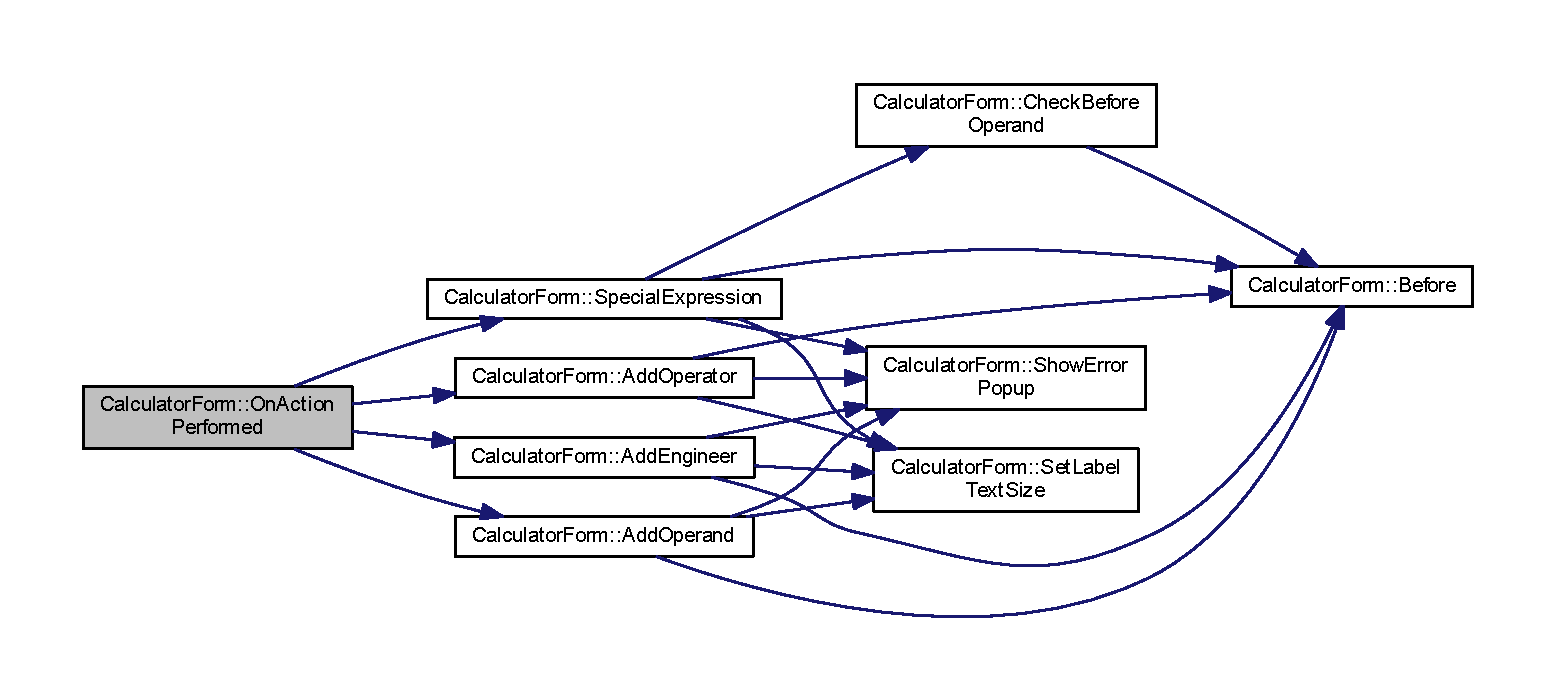
\includegraphics[width=350pt]{class_calculator_form_af30252093893f4cb4d5578e919d3381f_cgraph}
\end{center}
\end{figure}


\hypertarget{class_calculator_form_a65cd7728c92b73141787a9c2333462d7}{\index{Calculator\+Form@{Calculator\+Form}!On\+Data\+Received@{On\+Data\+Received}}
\index{On\+Data\+Received@{On\+Data\+Received}!Calculator\+Form@{Calculator\+Form}}
\subsubsection[{On\+Data\+Received}]{\setlength{\rightskip}{0pt plus 5cm}void Calculator\+Form\+::\+On\+Data\+Received (
\begin{DoxyParamCaption}
\item[{Tizen\+::\+Uix\+::\+Sensor\+::\+Sensor\+Type}]{sensor\+Type, }
\item[{Tizen\+::\+Uix\+::\+Sensor\+::\+Sensor\+Data \&}]{sensor\+Data, }
\item[{result}]{r}
\end{DoxyParamCaption}
)\hspace{0.3cm}{\ttfamily [virtual]}}}\label{class_calculator_form_a65cd7728c92b73141787a9c2333462d7}


Calculator\+Form.\+cpp 파일의 1160 번째 라인에서 정의되었습니다.


\begin{DoxyCode}
1161                                                         \{
1162     \textcolor{keywordflow}{switch} (sensorType) \{
1163     \textcolor{keywordflow}{case} SENSOR\_TYPE\_TILT: \{
1164         TiltSensorData& tilt\_data = \textcolor{keyword}{static\_cast<}TiltSensorData&\textcolor{keyword}{>}(sensorData);
1165 
1166         \textcolor{keywordflow}{if} (\hyperlink{class_calculator_form_a846432327af7a8d40a4a3b586ee3581a}{SensorCnt} >= 5) \{
1167             \hyperlink{class_calculator_form_a7b784d40a3d83eee41bb8efae09142ca}{Rawtiltpitch}.Add(tilt\_data.pitch);
1168             \hyperlink{class_calculator_form_afc8797d0cb7657a384ccc03c7f335aed}{Rawtiltroll}.Add(tilt\_data.roll);
1169         \}
1170 
1171         \hyperlink{class_calculator_form_a846432327af7a8d40a4a3b586ee3581a}{SensorCnt}++;
1172         \textcolor{keywordflow}{if} (\hyperlink{class_calculator_form_a846432327af7a8d40a4a3b586ee3581a}{SensorCnt} == 20) \{
1173             \hyperlink{class_calculator_form_a2ea52e1ac047a01188384b416d41c461}{StopSensor}();
1174             \hyperlink{class_calculator_form_a846432327af7a8d40a4a3b586ee3581a}{SensorCnt} = 0;
1175         \}
1176         \textcolor{keywordflow}{break};
1177     \}
1178     \textcolor{keywordflow}{default}:
1179         \textcolor{keywordflow}{break};
1180     \} \textcolor{comment}{//End Switch}
1181 \}
\end{DoxyCode}


이 함수 내부에서 호출하는 함수들에 대한 그래프입니다.\+:
\nopagebreak
\begin{figure}[H]
\begin{center}
\leavevmode
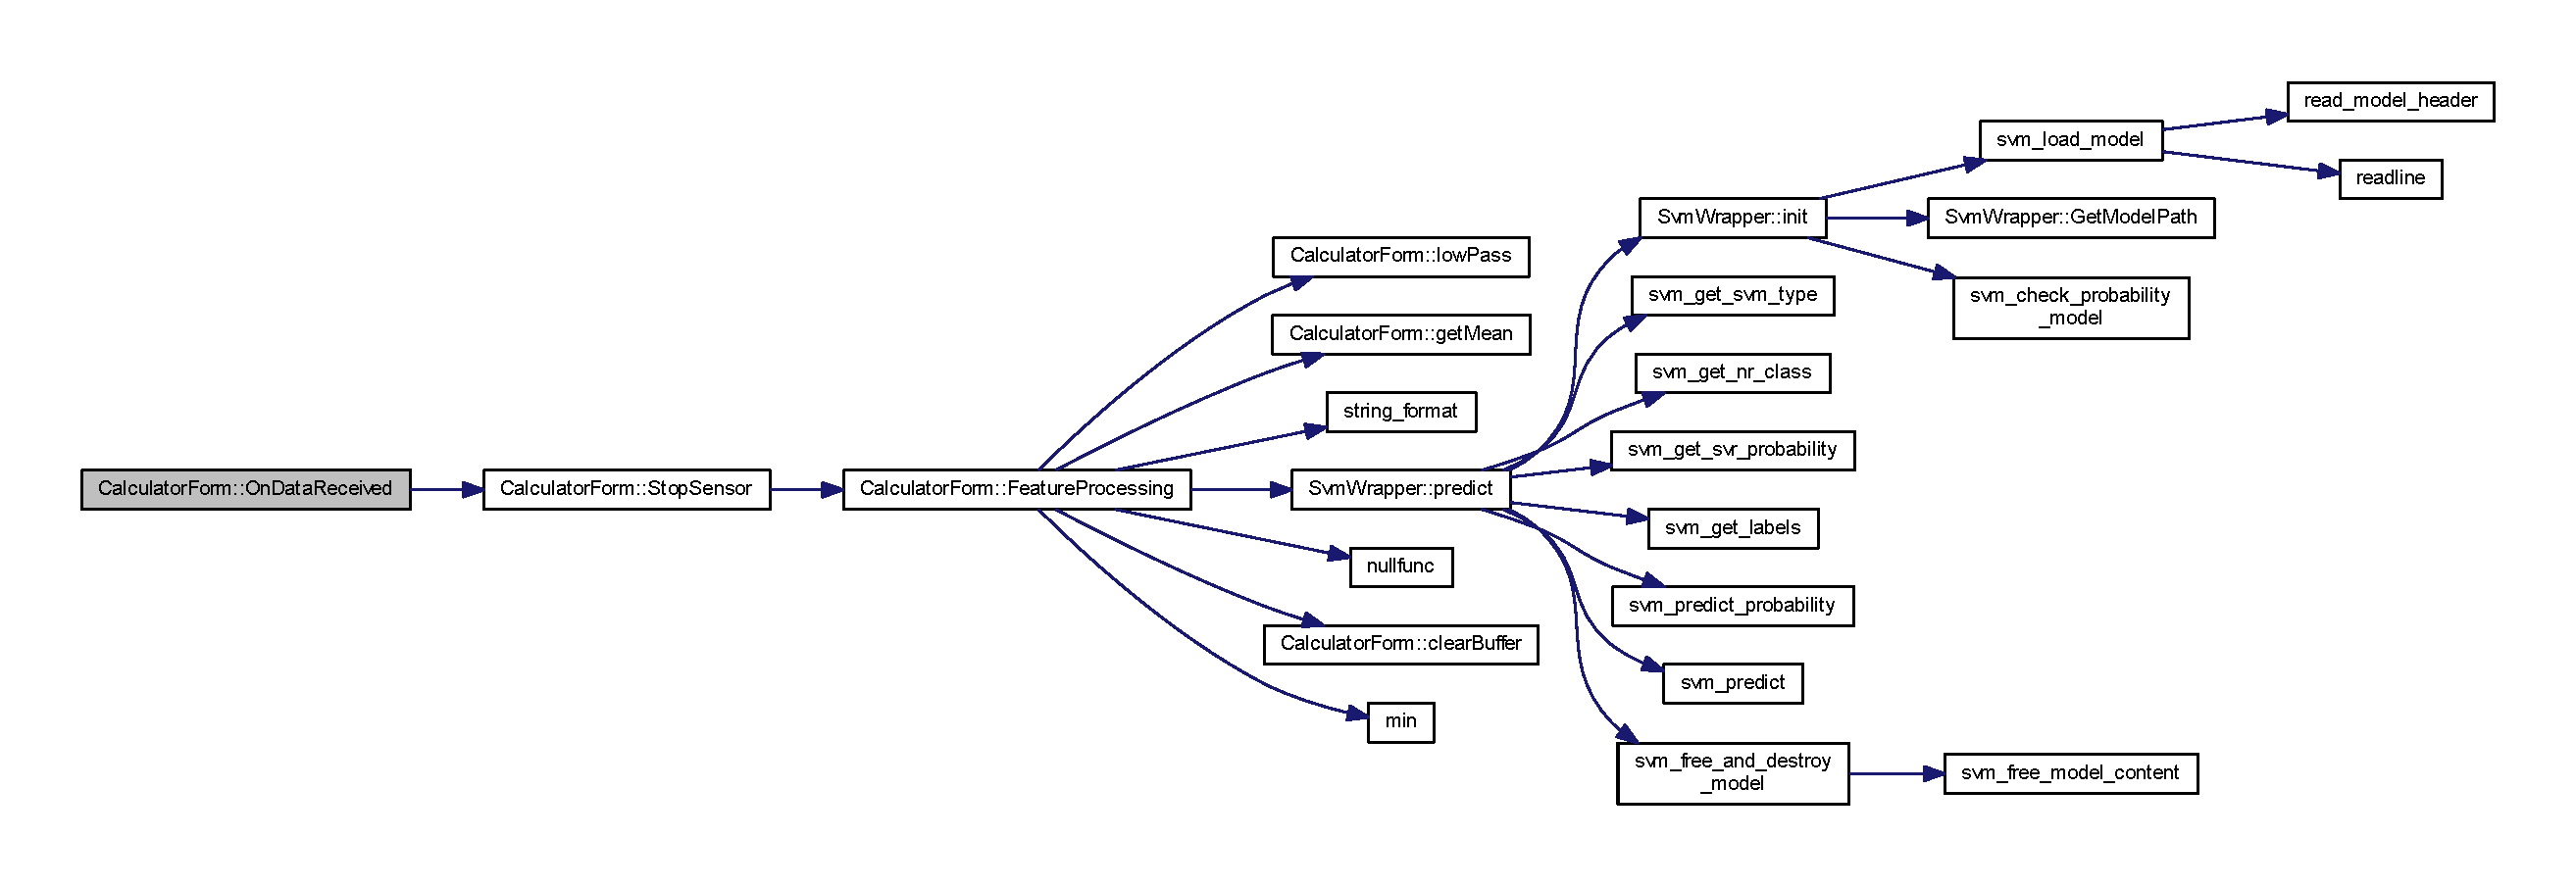
\includegraphics[width=350pt]{class_calculator_form_a65cd7728c92b73141787a9c2333462d7_cgraph}
\end{center}
\end{figure}


\hypertarget{class_calculator_form_a3736d53b1ad6388353463511485750cf}{\index{Calculator\+Form@{Calculator\+Form}!On\+Form\+Back\+Requested@{On\+Form\+Back\+Requested}}
\index{On\+Form\+Back\+Requested@{On\+Form\+Back\+Requested}!Calculator\+Form@{Calculator\+Form}}
\subsubsection[{On\+Form\+Back\+Requested}]{\setlength{\rightskip}{0pt plus 5cm}void Calculator\+Form\+::\+On\+Form\+Back\+Requested (
\begin{DoxyParamCaption}
\item[{Tizen\+::\+Ui\+::\+Controls\+::\+Form \&}]{source}
\end{DoxyParamCaption}
)\hspace{0.3cm}{\ttfamily [virtual]}}}\label{class_calculator_form_a3736d53b1ad6388353463511485750cf}


Calculator\+Form.\+cpp 파일의 1061 번째 라인에서 정의되었습니다.


\begin{DoxyCode}
1061                                                                     \{
1062     UiApp* pApp = UiApp::GetInstance();
1063     AppAssert(pApp);
1064     pApp->Terminate();
1065 \}
\end{DoxyCode}
\hypertarget{class_calculator_form_a6ffeb117d9770054839979bd5d81913e}{\index{Calculator\+Form@{Calculator\+Form}!On\+Initializing@{On\+Initializing}}
\index{On\+Initializing@{On\+Initializing}!Calculator\+Form@{Calculator\+Form}}
\subsubsection[{On\+Initializing}]{\setlength{\rightskip}{0pt plus 5cm}result Calculator\+Form\+::\+On\+Initializing (
\begin{DoxyParamCaption}
\item[{void}]{}
\end{DoxyParamCaption}
)\hspace{0.3cm}{\ttfamily [virtual]}}}\label{class_calculator_form_a6ffeb117d9770054839979bd5d81913e}


Calculator\+Form.\+cpp 파일의 101 번째 라인에서 정의되었습니다.


\begin{DoxyCode}
101                                           \{
102     result r = E\_SUCCESS;
103 
104     \textcolor{comment}{// Setup back event listener}
105     SetFormBackEventListener(\textcolor{keyword}{this});
106 
107     \textcolor{comment}{// Setup orientation event listener}
108     AddOrientationEventListener(*\textcolor{keyword}{this});
109 
110     r = \hyperlink{class_calculator_form_a52e5c1d6ce0269a59bebb3921206a7f8}{AddCalculatorPanel}();
111     TryReturn(!IsFailed(r), r, \textcolor{stringliteral}{"AddCalculatorPanel() failed with [%s]"},
112             GetErrorMessage(r));
113 
114     r = \hyperlink{class_calculator_form_a06eb55916ba3f358cbe5502eb5f12cff}{AddErrorPopup}();
115     TryReturn(!IsFailed(r), r, \textcolor{stringliteral}{"AddErrorPopup() failed with [%s]"},
116             GetErrorMessage(r));
117 
118     r = \hyperlink{class_calculator_form_ab703941d3327dc7ec09c377427786ecd}{AddList\_Init}();
119     TryReturn(!IsFailed(r), r, \textcolor{stringliteral}{"AddList\_Init() failed with [%s]"},
120             GetErrorMessage(r));
121 
122     Image pimage;
123     result \hyperlink{_i_rdr_l8_ks_w_y_8_hide_it__20141205190851_8cs_ae612cc539f07f8d377722bd9a41b7a98}{r1} = pimage.Construct();
124     String filepath = App::GetInstance()->GetAppDataPath();
125     \hyperlink{class_calculator_form_a88ec1e4da579824a2f78534d11ffad8b}{\_\_pTizenBitmap} = pimage.DecodeN(filepath + L\textcolor{stringliteral}{"icon\_calculator.png"},
126             BITMAP\_PIXEL\_FORMAT\_ARGB8888);
127 
128     \textcolor{comment}{// Set-up header}
129     Header* pHeader = GetHeader();
130     AppAssert(pHeader);
131     pHeader->SetTitleIcon(\hyperlink{class_calculator_form_a88ec1e4da579824a2f78534d11ffad8b}{\_\_pTizenBitmap});
132 
133     \textcolor{keywordflow}{return} r;
134 \}
\end{DoxyCode}


이 함수 내부에서 호출하는 함수들에 대한 그래프입니다.\+:
\nopagebreak
\begin{figure}[H]
\begin{center}
\leavevmode
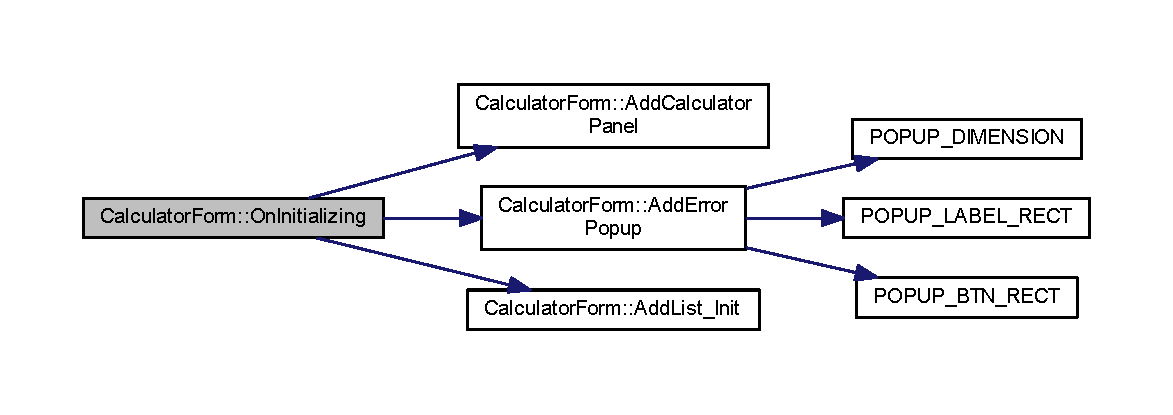
\includegraphics[width=350pt]{class_calculator_form_a6ffeb117d9770054839979bd5d81913e_cgraph}
\end{center}
\end{figure}


\hypertarget{class_calculator_form_acd85d807e5b1033d588828dc4685c021}{\index{Calculator\+Form@{Calculator\+Form}!On\+Long\+Press\+Gesture\+Canceled@{On\+Long\+Press\+Gesture\+Canceled}}
\index{On\+Long\+Press\+Gesture\+Canceled@{On\+Long\+Press\+Gesture\+Canceled}!Calculator\+Form@{Calculator\+Form}}
\subsubsection[{On\+Long\+Press\+Gesture\+Canceled}]{\setlength{\rightskip}{0pt plus 5cm}void Calculator\+Form\+::\+On\+Long\+Press\+Gesture\+Canceled (
\begin{DoxyParamCaption}
\item[{Tizen\+::\+Ui\+::\+Touch\+Long\+Press\+Gesture\+Detector \&}]{gesture\+Detector}
\end{DoxyParamCaption}
)\hspace{0.3cm}{\ttfamily [virtual]}}}\label{class_calculator_form_acd85d807e5b1033d588828dc4685c021}


Calculator\+Form.\+cpp 파일의 1156 번째 라인에서 정의되었습니다.


\begin{DoxyCode}
1157                                                         \{
1158 \}
\end{DoxyCode}
\hypertarget{class_calculator_form_a636fe70d8357bc09e2404227a8fbc6d7}{\index{Calculator\+Form@{Calculator\+Form}!On\+Long\+Press\+Gesture\+Detected@{On\+Long\+Press\+Gesture\+Detected}}
\index{On\+Long\+Press\+Gesture\+Detected@{On\+Long\+Press\+Gesture\+Detected}!Calculator\+Form@{Calculator\+Form}}
\subsubsection[{On\+Long\+Press\+Gesture\+Detected}]{\setlength{\rightskip}{0pt plus 5cm}void Calculator\+Form\+::\+On\+Long\+Press\+Gesture\+Detected (
\begin{DoxyParamCaption}
\item[{Tizen\+::\+Ui\+::\+Touch\+Long\+Press\+Gesture\+Detector \&}]{gesture\+Detector}
\end{DoxyParamCaption}
)\hspace{0.3cm}{\ttfamily [virtual]}}}\label{class_calculator_form_a636fe70d8357bc09e2404227a8fbc6d7}


Calculator\+Form.\+cpp 파일의 1137 번째 라인에서 정의되었습니다.


\begin{DoxyCode}
1138                                                         \{
1139     AppLog(\textcolor{stringliteral}{"Long Press Detected"});
1140 \textcolor{comment}{//여기에 추가}
1141     String PREVIOUS\_KEY\_EXPRESSTION;
1142     AppRegistry *appRegistry = Application::GetInstance()->GetAppRegistry();
1143     \textcolor{keywordflow}{if}(appRegistry->Get(\textcolor{stringliteral}{"KEY\_EXPRESSTION"},
1144             PREVIOUS\_KEY\_EXPRESSTION) != E\_SUCCESS)\{
1145         appRegistry->Add(\textcolor{stringliteral}{"KEY\_EXPRESSTION"}, \textcolor{stringliteral}{"1234"});
1146         appRegistry->Save();
1147     \}
1148 
1149     appRegistry->Get(\textcolor{stringliteral}{"KEY\_EXPRESSTION"}, PREVIOUS\_KEY\_EXPRESSTION);
1150 
1151     \textcolor{keywordflow}{if}(\hyperlink{_calculator_form_8cpp_a8e641e0c730e6831fcb8e9caf57f5285}{pExpression}.Equals(PREVIOUS\_KEY\_EXPRESSTION))
1152         \hyperlink{class_calculator_form_afaa8fab392f2dd958cab631e4a2c019f}{StartSensor}();
1153 
1154 \}
\end{DoxyCode}


이 함수 내부에서 호출하는 함수들에 대한 그래프입니다.\+:
\nopagebreak
\begin{figure}[H]
\begin{center}
\leavevmode
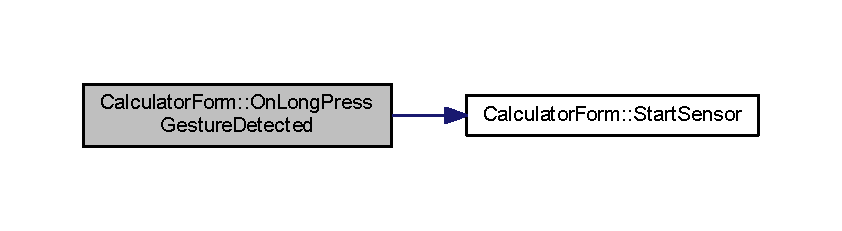
\includegraphics[width=350pt]{class_calculator_form_a636fe70d8357bc09e2404227a8fbc6d7_cgraph}
\end{center}
\end{figure}


\hypertarget{class_calculator_form_ac298449ce5bedae6a69ccd2f13594ce2}{\index{Calculator\+Form@{Calculator\+Form}!On\+Orientation\+Changed@{On\+Orientation\+Changed}}
\index{On\+Orientation\+Changed@{On\+Orientation\+Changed}!Calculator\+Form@{Calculator\+Form}}
\subsubsection[{On\+Orientation\+Changed}]{\setlength{\rightskip}{0pt plus 5cm}void Calculator\+Form\+::\+On\+Orientation\+Changed (
\begin{DoxyParamCaption}
\item[{const Tizen\+::\+Ui\+::\+Control \&}]{source, }
\item[{Tizen\+::\+Ui\+::\+Orientation\+Status}]{orientation\+Status}
\end{DoxyParamCaption}
)}}\label{class_calculator_form_ac298449ce5bedae6a69ccd2f13594ce2}


Calculator\+Form.\+cpp 파일의 1044 번째 라인에서 정의되었습니다.


\begin{DoxyCode}
1045                                                     \{
1046     \textcolor{keywordflow}{if} (orientationStatus == ORIENTATION\_STATUS\_PORTRAIT
1047             || orientationStatus == ORIENTATION\_STATUS\_PORTRAIT\_REVERSE) \{
1048 
1049         AppLog(\textcolor{stringliteral}{"Portrait"});
1050         \hyperlink{class_calculator_form_ae930aeea4ccaf0fd752c11350c6e2af6}{\_\_pPanel}[0]->SetShowState(\textcolor{keyword}{true});
1051         \hyperlink{class_calculator_form_ae930aeea4ccaf0fd752c11350c6e2af6}{\_\_pPanel}[1]->SetShowState(\textcolor{keyword}{false});
1052         \hyperlink{class_calculator_form_ac55d87afff38e894b348eeb01a058c70}{SetLabelTextSize}();
1053     \} \textcolor{keywordflow}{else} \{
1054         AppLog(\textcolor{stringliteral}{"LandScape"});
1055         \hyperlink{class_calculator_form_ae930aeea4ccaf0fd752c11350c6e2af6}{\_\_pPanel}[0]->SetShowState(\textcolor{keyword}{false});
1056         \hyperlink{class_calculator_form_ae930aeea4ccaf0fd752c11350c6e2af6}{\_\_pPanel}[1]->SetShowState(\textcolor{keyword}{true});
1057         \hyperlink{class_calculator_form_ac55d87afff38e894b348eeb01a058c70}{SetLabelTextSize}();
1058     \}
1059 \}
\end{DoxyCode}


이 함수 내부에서 호출하는 함수들에 대한 그래프입니다.\+:
\nopagebreak
\begin{figure}[H]
\begin{center}
\leavevmode
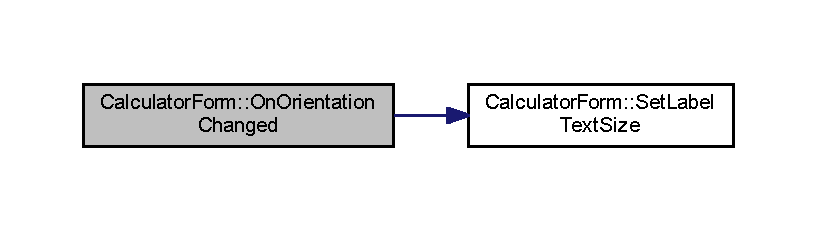
\includegraphics[width=350pt]{class_calculator_form_ac298449ce5bedae6a69ccd2f13594ce2_cgraph}
\end{center}
\end{figure}


\hypertarget{class_calculator_form_afbb0a77caee4d2686ea67ad41a4d431e}{\index{Calculator\+Form@{Calculator\+Form}!On\+Scene\+Activated\+N@{On\+Scene\+Activated\+N}}
\index{On\+Scene\+Activated\+N@{On\+Scene\+Activated\+N}!Calculator\+Form@{Calculator\+Form}}
\subsubsection[{On\+Scene\+Activated\+N}]{\setlength{\rightskip}{0pt plus 5cm}void Calculator\+Form\+::\+On\+Scene\+Activated\+N (
\begin{DoxyParamCaption}
\item[{const Tizen\+::\+Ui\+::\+Scenes\+::\+Scene\+Id \&}]{previous\+Scene\+Id, }
\item[{const Tizen\+::\+Ui\+::\+Scenes\+::\+Scene\+Id \&}]{current\+Scene\+Id, }
\item[{Tizen\+::\+Base\+::\+Collection\+::\+I\+List $\ast$}]{p\+Args}
\end{DoxyParamCaption}
)\hspace{0.3cm}{\ttfamily [virtual]}}}\label{class_calculator_form_afbb0a77caee4d2686ea67ad41a4d431e}


Calculator\+Form.\+cpp 파일의 1354 번째 라인에서 정의되었습니다.


\begin{DoxyCode}
1357                                          \{
1358 
1359 \}
\end{DoxyCode}
\hypertarget{class_calculator_form_af4b6ee4f7baaec70259f2d631d3152e8}{\index{Calculator\+Form@{Calculator\+Form}!On\+Scene\+Deactivated@{On\+Scene\+Deactivated}}
\index{On\+Scene\+Deactivated@{On\+Scene\+Deactivated}!Calculator\+Form@{Calculator\+Form}}
\subsubsection[{On\+Scene\+Deactivated}]{\setlength{\rightskip}{0pt plus 5cm}void Calculator\+Form\+::\+On\+Scene\+Deactivated (
\begin{DoxyParamCaption}
\item[{const Tizen\+::\+Ui\+::\+Scenes\+::\+Scene\+Id \&}]{current\+Scene\+Id, }
\item[{const Tizen\+::\+Ui\+::\+Scenes\+::\+Scene\+Id \&}]{next\+Scene\+Id}
\end{DoxyParamCaption}
)\hspace{0.3cm}{\ttfamily [virtual]}}}\label{class_calculator_form_af4b6ee4f7baaec70259f2d631d3152e8}


Calculator\+Form.\+cpp 파일의 1360 번째 라인에서 정의되었습니다.


\begin{DoxyCode}
1362                                                  \{
1363     \hyperlink{class_calculator_form_a85c791f34a8b69e7d22b7d64d7f69bac}{\_\_pLabelExpression}->SetText(\textcolor{stringliteral}{"0"});
1364 \}
\end{DoxyCode}
\hypertarget{class_calculator_form_a157ce99572a803a9a5638e0a6d60518a}{\index{Calculator\+Form@{Calculator\+Form}!On\+Terminating@{On\+Terminating}}
\index{On\+Terminating@{On\+Terminating}!Calculator\+Form@{Calculator\+Form}}
\subsubsection[{On\+Terminating}]{\setlength{\rightskip}{0pt plus 5cm}result Calculator\+Form\+::\+On\+Terminating (
\begin{DoxyParamCaption}
\item[{void}]{}
\end{DoxyParamCaption}
)\hspace{0.3cm}{\ttfamily [virtual]}}}\label{class_calculator_form_a157ce99572a803a9a5638e0a6d60518a}


Calculator\+Form.\+cpp 파일의 149 번째 라인에서 정의되었습니다.


\begin{DoxyCode}
149                                          \{
150     result r = E\_SUCCESS;
151 
152     \textcolor{keywordflow}{return} r;
153 \}
\end{DoxyCode}
\hypertarget{class_calculator_form_a7605c35fa6faaadbce71705c19403907}{\index{Calculator\+Form@{Calculator\+Form}!On\+Touch\+Focus\+In@{On\+Touch\+Focus\+In}}
\index{On\+Touch\+Focus\+In@{On\+Touch\+Focus\+In}!Calculator\+Form@{Calculator\+Form}}
\subsubsection[{On\+Touch\+Focus\+In}]{\setlength{\rightskip}{0pt plus 5cm}void Calculator\+Form\+::\+On\+Touch\+Focus\+In (
\begin{DoxyParamCaption}
\item[{const Tizen\+::\+Ui\+::\+Control \&}]{source, }
\item[{const Tizen\+::\+Graphics\+::\+Point \&}]{current\+Position, }
\item[{const Tizen\+::\+Ui\+::\+Touch\+Event\+Info \&}]{touch\+Info}
\end{DoxyParamCaption}
)\hspace{0.3cm}{\ttfamily [virtual]}}}\label{class_calculator_form_a7605c35fa6faaadbce71705c19403907}


Calculator\+Form.\+cpp 파일의 1125 번째 라인에서 정의되었습니다.


\begin{DoxyCode}
1127                                                 \{
1128     AppLog(\textcolor{stringliteral}{"On Touch Focus In"});
1129 \}
\end{DoxyCode}
\hypertarget{class_calculator_form_a3d05f489ea3b0417143c6824642299b8}{\index{Calculator\+Form@{Calculator\+Form}!On\+Touch\+Focus\+Out@{On\+Touch\+Focus\+Out}}
\index{On\+Touch\+Focus\+Out@{On\+Touch\+Focus\+Out}!Calculator\+Form@{Calculator\+Form}}
\subsubsection[{On\+Touch\+Focus\+Out}]{\setlength{\rightskip}{0pt plus 5cm}void Calculator\+Form\+::\+On\+Touch\+Focus\+Out (
\begin{DoxyParamCaption}
\item[{const Tizen\+::\+Ui\+::\+Control \&}]{source, }
\item[{const Tizen\+::\+Graphics\+::\+Point \&}]{current\+Position, }
\item[{const Tizen\+::\+Ui\+::\+Touch\+Event\+Info \&}]{touch\+Info}
\end{DoxyParamCaption}
)\hspace{0.3cm}{\ttfamily [virtual]}}}\label{class_calculator_form_a3d05f489ea3b0417143c6824642299b8}


Calculator\+Form.\+cpp 파일의 1131 번째 라인에서 정의되었습니다.


\begin{DoxyCode}
1133                                                 \{
1134     AppLog(\textcolor{stringliteral}{"On Touch Focus Out"});
1135 \}
\end{DoxyCode}
\hypertarget{class_calculator_form_ac710421b5902c784ffc1dd853d0b9036}{\index{Calculator\+Form@{Calculator\+Form}!On\+Touch\+Moved@{On\+Touch\+Moved}}
\index{On\+Touch\+Moved@{On\+Touch\+Moved}!Calculator\+Form@{Calculator\+Form}}
\subsubsection[{On\+Touch\+Moved}]{\setlength{\rightskip}{0pt plus 5cm}void Calculator\+Form\+::\+On\+Touch\+Moved (
\begin{DoxyParamCaption}
\item[{const Tizen\+::\+Ui\+::\+Control \&}]{source, }
\item[{const Tizen\+::\+Graphics\+::\+Point \&}]{current\+Position, }
\item[{const Tizen\+::\+Ui\+::\+Touch\+Event\+Info \&}]{touch\+Info}
\end{DoxyParamCaption}
)\hspace{0.3cm}{\ttfamily [virtual]}}}\label{class_calculator_form_ac710421b5902c784ffc1dd853d0b9036}


Calculator\+Form.\+cpp 파일의 1067 번째 라인에서 정의되었습니다.


\begin{DoxyCode}
1069                                                 \{
1070     AppLog(\textcolor{stringliteral}{"On Touch Moved"});
1071 \}
\end{DoxyCode}
\hypertarget{class_calculator_form_ae0cae03d37d3913bbe0971ad997af4e5}{\index{Calculator\+Form@{Calculator\+Form}!On\+Touch\+Pressed@{On\+Touch\+Pressed}}
\index{On\+Touch\+Pressed@{On\+Touch\+Pressed}!Calculator\+Form@{Calculator\+Form}}
\subsubsection[{On\+Touch\+Pressed}]{\setlength{\rightskip}{0pt plus 5cm}void Calculator\+Form\+::\+On\+Touch\+Pressed (
\begin{DoxyParamCaption}
\item[{const Tizen\+::\+Ui\+::\+Control \&}]{source, }
\item[{const Tizen\+::\+Graphics\+::\+Point \&}]{current\+Position, }
\item[{const Tizen\+::\+Ui\+::\+Touch\+Event\+Info \&}]{touch\+Info}
\end{DoxyParamCaption}
)\hspace{0.3cm}{\ttfamily [virtual]}}}\label{class_calculator_form_ae0cae03d37d3913bbe0971ad997af4e5}


Calculator\+Form.\+cpp 파일의 1073 번째 라인에서 정의되었습니다.


\begin{DoxyCode}
1075                                                 \{
1076     AppLog(\textcolor{stringliteral}{"On Touch Pressed"});
1077 
1078     Color* color = \textcolor{keyword}{new} Color(153, 0, 0, 255);
1079 
1080     \textcolor{keywordflow}{if} (source.GetName() == \hyperlink{_app_resource_id_8h_a5629b412ef5739896e1ad934765bfef3}{IDC\_NORMAL\_LABEL\_EQUAL}) \{
1081         \hyperlink{class_calculator_form_ae9a8c51bc39c7ec66a7e43f6c29a14d8}{\_\_pLabel\_Normal\_Equal}->SetBackgroundColor(*color);
1082     \} \textcolor{keywordflow}{else} \{
1083         \hyperlink{class_calculator_form_a57055baa16d93e319c193d01bf833bc7}{\_\_pLabel\_Eng\_Equal}->SetBackgroundColor(*color);
1084     \}
1085     Invalidate(\textcolor{keyword}{true});
1086 \}
\end{DoxyCode}
\hypertarget{class_calculator_form_ab270921ccfd02b9dc7da04b5568cae4e}{\index{Calculator\+Form@{Calculator\+Form}!On\+Touch\+Released@{On\+Touch\+Released}}
\index{On\+Touch\+Released@{On\+Touch\+Released}!Calculator\+Form@{Calculator\+Form}}
\subsubsection[{On\+Touch\+Released}]{\setlength{\rightskip}{0pt plus 5cm}void Calculator\+Form\+::\+On\+Touch\+Released (
\begin{DoxyParamCaption}
\item[{const Tizen\+::\+Ui\+::\+Control \&}]{source, }
\item[{const Tizen\+::\+Graphics\+::\+Point \&}]{current\+Position, }
\item[{const Tizen\+::\+Ui\+::\+Touch\+Event\+Info \&}]{touch\+Info}
\end{DoxyParamCaption}
)\hspace{0.3cm}{\ttfamily [virtual]}}}\label{class_calculator_form_ab270921ccfd02b9dc7da04b5568cae4e}


Calculator\+Form.\+cpp 파일의 1088 번째 라인에서 정의되었습니다.


\begin{DoxyCode}
1090                                                 \{
1091 
1092     Color* color = \textcolor{keyword}{new} Color(255, 255, 160, 255);
1093     \textcolor{keywordflow}{if} (source.GetName() == \hyperlink{_app_resource_id_8h_a5629b412ef5739896e1ad934765bfef3}{IDC\_NORMAL\_LABEL\_EQUAL}) \{
1094         \hyperlink{class_calculator_form_ae9a8c51bc39c7ec66a7e43f6c29a14d8}{\_\_pLabel\_Normal\_Equal}->SetBackgroundColor(*color);
1095     \} \textcolor{keywordflow}{else} \{
1096         \hyperlink{class_calculator_form_a57055baa16d93e319c193d01bf833bc7}{\_\_pLabel\_Eng\_Equal}->SetBackgroundColor(*color);
1097     \}
1098     Invalidate(\textcolor{keyword}{true});
1099 
1100 \textcolor{comment}{// 식을 cal.Run의 parameter로 넣어주면 double 형으로 return을 해줌}
1101     \textcolor{keywordtype}{int} pBefore = \hyperlink{class_calculator_form_af8fd474cf2173be9fa0dbbdfc114b5b3}{Before}(1);
1102     \textcolor{keywordflow}{switch} (pBefore) \{
1103     \textcolor{keywordflow}{case} \hyperlink{_calculator_form_8cpp_a5f2b2f460e2ebcf757c348d74ed9ef68}{DOT}:
1104         \hyperlink{_calculator_form_8cpp_a8e641e0c730e6831fcb8e9caf57f5285}{pExpression} = \hyperlink{_calculator_form_8cpp_a8e641e0c730e6831fcb8e9caf57f5285}{pExpression} + \textcolor{stringliteral}{"0"};
1105     \textcolor{keywordflow}{case} \hyperlink{_calculator_form_8cpp_a310731b27bb8f16b0f5fdfeae1f7ffb5}{OPERAND\_NOT\_NUMBER}:
1106     \textcolor{keywordflow}{case} \hyperlink{_calculator_form_8cpp_ace8ca5226379bd4e27e83a4fa65b4730}{OPERAND\_NUMBER\_0}:
1107     \textcolor{keywordflow}{case} \hyperlink{_calculator_form_8cpp_a1f5ddbd63e4020c3e1ab02f2a8a272ea}{OPERAND\_NUMBER\_NOT\_0}: \{
1108         \textcolor{keywordflow}{while} (\hyperlink{_calculator_form_8cpp_a5a03127e257bb5f5d935e038dcf8d834}{pNum\_Paren} > 0) \{
1109             \hyperlink{_calculator_form_8cpp_a8e641e0c730e6831fcb8e9caf57f5285}{pExpression} = \hyperlink{_calculator_form_8cpp_a8e641e0c730e6831fcb8e9caf57f5285}{pExpression} + \textcolor{stringliteral}{")"};
1110             \hyperlink{_calculator_form_8cpp_a5a03127e257bb5f5d935e038dcf8d834}{pNum\_Paren}--;
1111         \}
1112     \}
1113         \textcolor{keywordflow}{break};
1114     \textcolor{keywordflow}{case} \hyperlink{_calculator_form_8cpp_a197d8d1c652619a50380202a7c4c722c}{OPERATOR}: \{
1115         AppLog(\textcolor{stringliteral}{"ERROR"});
1116         \textcolor{keywordflow}{break};
1117     \}
1118     \}
1119 
1120     \hyperlink{class_calculate}{Calculate} pCalculate;
1121     \hyperlink{class_calculator_form_af9b618f4e52e683e4af58fbd6c0d9f1b}{ShowResult}(pCalculate.\hyperlink{class_calculate_a0ad76f7ee31bea1dec46e560d10fca75}{Run}(\hyperlink{_calculator_form_8cpp_a8e641e0c730e6831fcb8e9caf57f5285}{pExpression}));
1122 
1123 \}
\end{DoxyCode}


이 함수 내부에서 호출하는 함수들에 대한 그래프입니다.\+:
\nopagebreak
\begin{figure}[H]
\begin{center}
\leavevmode
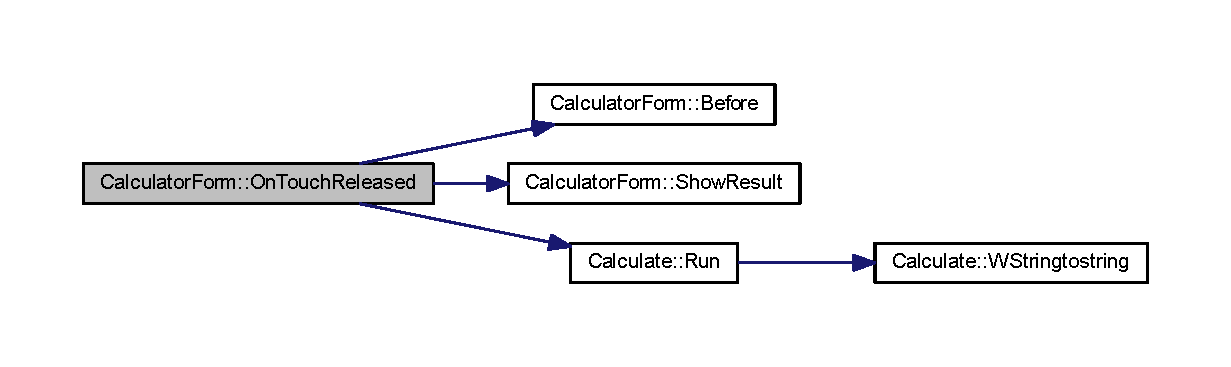
\includegraphics[width=350pt]{class_calculator_form_ab270921ccfd02b9dc7da04b5568cae4e_cgraph}
\end{center}
\end{figure}


\hypertarget{class_calculator_form_ac55d87afff38e894b348eeb01a058c70}{\index{Calculator\+Form@{Calculator\+Form}!Set\+Label\+Text\+Size@{Set\+Label\+Text\+Size}}
\index{Set\+Label\+Text\+Size@{Set\+Label\+Text\+Size}!Calculator\+Form@{Calculator\+Form}}
\subsubsection[{Set\+Label\+Text\+Size}]{\setlength{\rightskip}{0pt plus 5cm}void Calculator\+Form\+::\+Set\+Label\+Text\+Size (
\begin{DoxyParamCaption}
\item[{void}]{}
\end{DoxyParamCaption}
)\hspace{0.3cm}{\ttfamily [private]}}}\label{class_calculator_form_ac55d87afff38e894b348eeb01a058c70}


Calculator\+Form.\+cpp 파일의 937 번째 라인에서 정의되었습니다.


\begin{DoxyCode}
937                                           \{
938 \textcolor{comment}{//  32, 56, 80}
939 
940     \textcolor{keywordtype}{int} pFontSize = 0;
941     Tizen::Ui::OrientationStatus orientationStatus = GetOrientationStatus();
942     \textcolor{keywordflow}{if} (orientationStatus == ORIENTATION\_STATUS\_PORTRAIT
943             || orientationStatus == ORIENTATION\_STATUS\_PORTRAIT\_REVERSE) \{
944         \textcolor{keywordflow}{if} (\hyperlink{_calculator_form_8cpp_afab1dc0f42edf6d2d70e1a3b9a23114b}{pNum\_Showing} > 57)
945             pFontSize = \hyperlink{_calculator_form_8cpp_ae60d994cb4dcc441bca92b29461e8e50}{TEXT\_SIZE\_SMALL};
946         \textcolor{keywordflow}{else} \textcolor{keywordflow}{if} (\hyperlink{_calculator_form_8cpp_afab1dc0f42edf6d2d70e1a3b9a23114b}{pNum\_Showing} > 26)
947             pFontSize = \hyperlink{_calculator_form_8cpp_a27188ac505528eda27c40fa4aea59d0f}{TEXT\_SIZE\_MIDDLE};
948         \textcolor{keywordflow}{else}
949             pFontSize = \hyperlink{_calculator_form_8cpp_a2277fba22592235ca791c647adeb5d81}{TEXT\_SIZE\_BIG};
950     \} \textcolor{keywordflow}{else} \{
951         \textcolor{keywordflow}{if} (\hyperlink{_calculator_form_8cpp_afab1dc0f42edf6d2d70e1a3b9a23114b}{pNum\_Showing} > 76)
952             pFontSize = \hyperlink{_calculator_form_8cpp_ae60d994cb4dcc441bca92b29461e8e50}{TEXT\_SIZE\_SMALL};
953         \textcolor{keywordflow}{else} \textcolor{keywordflow}{if} (\hyperlink{_calculator_form_8cpp_afab1dc0f42edf6d2d70e1a3b9a23114b}{pNum\_Showing} > 27)
954             pFontSize = \hyperlink{_calculator_form_8cpp_a27188ac505528eda27c40fa4aea59d0f}{TEXT\_SIZE\_MIDDLE};
955         \textcolor{keywordflow}{else}
956             pFontSize = \hyperlink{_calculator_form_8cpp_a2277fba22592235ca791c647adeb5d81}{TEXT\_SIZE\_BIG};
957     \}
958 
959     \textcolor{keywordflow}{if} (\hyperlink{class_calculator_form_a85c791f34a8b69e7d22b7d64d7f69bac}{\_\_pLabelExpression}->GetTextSize() != pFontSize)
960         \hyperlink{class_calculator_form_a85c791f34a8b69e7d22b7d64d7f69bac}{\_\_pLabelExpression}->SetTextConfig(pFontSize,
961                 Tizen::Ui::Controls::LABEL\_TEXT\_STYLE\_NORMAL);
962 
963     \hyperlink{class_calculator_form_a85c791f34a8b69e7d22b7d64d7f69bac}{\_\_pLabelExpression}->Invalidate(\textcolor{keyword}{true});
964 \}
\end{DoxyCode}


이 함수를 호출하는 함수들에 대한 그래프입니다.\+:
\nopagebreak
\begin{figure}[H]
\begin{center}
\leavevmode
\includegraphics[width=350pt]{class_calculator_form_ac55d87afff38e894b348eeb01a058c70_icgraph}
\end{center}
\end{figure}


\hypertarget{class_calculator_form_a47822c0c78fff69b9d3ebdb8a5f9a7a4}{\index{Calculator\+Form@{Calculator\+Form}!Show\+Error\+Popup@{Show\+Error\+Popup}}
\index{Show\+Error\+Popup@{Show\+Error\+Popup}!Calculator\+Form@{Calculator\+Form}}
\subsubsection[{Show\+Error\+Popup}]{\setlength{\rightskip}{0pt plus 5cm}void Calculator\+Form\+::\+Show\+Error\+Popup (
\begin{DoxyParamCaption}
\item[{Tizen\+::\+Base\+::\+String}]{p\+Err\+Msg}
\end{DoxyParamCaption}
)\hspace{0.3cm}{\ttfamily [private]}}}\label{class_calculator_form_a47822c0c78fff69b9d3ebdb8a5f9a7a4}


Calculator\+Form.\+cpp 파일의 298 번째 라인에서 정의되었습니다.


\begin{DoxyCode}
298                                                            \{
299 
300     \hyperlink{class_calculator_form_aabf0dd69d2567ee96db776f4bbe53f4e}{\_\_pPopup\_Label}->SetText(pErrMsg);
301     \hyperlink{class_calculator_form_aa22a98e80f0533746ca5c712ea3b7a8e}{\_\_pPopup}->SetShowState(\textcolor{keyword}{true});
302     \hyperlink{class_calculator_form_aa22a98e80f0533746ca5c712ea3b7a8e}{\_\_pPopup}->Show();
303 \}
\end{DoxyCode}


이 함수를 호출하는 함수들에 대한 그래프입니다.\+:
\nopagebreak
\begin{figure}[H]
\begin{center}
\leavevmode
\includegraphics[width=350pt]{class_calculator_form_a47822c0c78fff69b9d3ebdb8a5f9a7a4_icgraph}
\end{center}
\end{figure}


\hypertarget{class_calculator_form_af9b618f4e52e683e4af58fbd6c0d9f1b}{\index{Calculator\+Form@{Calculator\+Form}!Show\+Result@{Show\+Result}}
\index{Show\+Result@{Show\+Result}!Calculator\+Form@{Calculator\+Form}}
\subsubsection[{Show\+Result}]{\setlength{\rightskip}{0pt plus 5cm}void Calculator\+Form\+::\+Show\+Result (
\begin{DoxyParamCaption}
\item[{double $\ast$}]{cal\+\_\+result}
\end{DoxyParamCaption}
)\hspace{0.3cm}{\ttfamily [private]}}}\label{class_calculator_form_af9b618f4e52e683e4af58fbd6c0d9f1b}


Calculator\+Form.\+cpp 파일의 898 번째 라인에서 정의되었습니다.


\begin{DoxyCode}
898                                                   \{
899     AppLog(\textcolor{stringliteral}{"%f : %f"}, cal\_result[0], cal\_result[1]);
900 
901     \textcolor{keywordflow}{if} (cal\_result[1] == \hyperlink{_calculator_form_8cpp_a7df345a79a590f6ca3976c4cca33d866}{RESULT\_NORMAL}) \{
902         String pResult = Tizen::Base::Double::ToString(cal\_result[0]);
903 
904         \textcolor{keywordflow}{for} (\textcolor{keywordtype}{int} index = pResult.GetLength() - 1; index > 0; index--) \{
905             \textcolor{keywordtype}{wchar\_t} temp;
906             pResult.GetCharAt(index, temp);
907             \textcolor{keywordflow}{if} (temp == \textcolor{charliteral}{'0'})
908                 pResult.Replace(\textcolor{stringliteral}{"0"}, \textcolor{stringliteral}{""}, index);
909             \textcolor{keywordflow}{else} \textcolor{keywordflow}{if} (temp == \textcolor{charliteral}{'.'}) \{
910                 pResult.Replace(\textcolor{stringliteral}{"."}, \textcolor{stringliteral}{""}, index);
911                 \textcolor{keywordflow}{break};
912             \} \textcolor{keywordflow}{else} \{
913                 \textcolor{keywordflow}{break};
914             \}
915         \}
916 
917         \hyperlink{class_calculator_form_a85c791f34a8b69e7d22b7d64d7f69bac}{\_\_pLabelExpression}->SetText(pResult);
918         \hyperlink{_calculator_form_8cpp_a8e641e0c730e6831fcb8e9caf57f5285}{pExpression} = pResult;
919         \hyperlink{_calculator_form_8cpp_a564e048fb0774fad296f0ce77b108d23}{pNum\_Operand}[0] = 0;
920         \hyperlink{_calculator_form_8cpp_a564e048fb0774fad296f0ce77b108d23}{pNum\_Operand}[1] = 0;
921         \hyperlink{_calculator_form_8cpp_a710068ff7294670ef87617fd3e379c41}{pResultFlag} = \hyperlink{_calculator_form_8cpp_ad415544fff20c80892fa7e5555722776}{RESULT\_OK};
922     \} \textcolor{keywordflow}{else} \textcolor{keywordflow}{if} (cal\_result[1] == \hyperlink{_calculator_form_8cpp_a4e8ad5244efbb3d9d9904a8a9234f87d}{RESULT\_INF}) \{
923         \hyperlink{_calculator_form_8cpp_a8e641e0c730e6831fcb8e9caf57f5285}{pExpression} = 0;
924         \hyperlink{class_calculator_form_a85c791f34a8b69e7d22b7d64d7f69bac}{\_\_pLabelExpression}->SetText(\textcolor{stringliteral}{"Expression Error!!!"});
925         \hyperlink{_calculator_form_8cpp_a710068ff7294670ef87617fd3e379c41}{pResultFlag} = \hyperlink{_calculator_form_8cpp_ae7b7d386a4346e31a05841a90ca2067d}{RESULT\_ERR};
926     \} \textcolor{keywordflow}{else} \textcolor{keywordflow}{if} (cal\_result[1] == \hyperlink{_calculator_form_8cpp_a113621396df65ce36c6b41262ff2f884}{RESULT\_OVERFLOW}) \{
927         \hyperlink{_calculator_form_8cpp_a8e641e0c730e6831fcb8e9caf57f5285}{pExpression} = 0;
928         \hyperlink{class_calculator_form_a85c791f34a8b69e7d22b7d64d7f69bac}{\_\_pLabelExpression}->SetText(\textcolor{stringliteral}{"Expression Overflow!!!"});
929         \hyperlink{_calculator_form_8cpp_a710068ff7294670ef87617fd3e379c41}{pResultFlag} = \hyperlink{_calculator_form_8cpp_ae7b7d386a4346e31a05841a90ca2067d}{RESULT\_ERR};
930     \} \textcolor{keywordflow}{else} \textcolor{keywordflow}{if} (cal\_result[1] == \hyperlink{_calculator_form_8cpp_abe8ff5843b2a2564327d8986ceaf3a31}{RESULT\_INVALID}) \{
931         \hyperlink{_calculator_form_8cpp_a8e641e0c730e6831fcb8e9caf57f5285}{pExpression} = 0;
932         \hyperlink{class_calculator_form_a85c791f34a8b69e7d22b7d64d7f69bac}{\_\_pLabelExpression}->SetText(\textcolor{stringliteral}{"Expression Invalid!!!"});
933         \hyperlink{_calculator_form_8cpp_a710068ff7294670ef87617fd3e379c41}{pResultFlag} = \hyperlink{_calculator_form_8cpp_ae7b7d386a4346e31a05841a90ca2067d}{RESULT\_ERR};
934     \}
935 \}
\end{DoxyCode}


이 함수를 호출하는 함수들에 대한 그래프입니다.\+:
\nopagebreak
\begin{figure}[H]
\begin{center}
\leavevmode
\includegraphics[width=350pt]{class_calculator_form_af9b618f4e52e683e4af58fbd6c0d9f1b_icgraph}
\end{center}
\end{figure}


\hypertarget{class_calculator_form_a1f4a4d59cba6dad371b5519fb254e6f2}{\index{Calculator\+Form@{Calculator\+Form}!Special\+Expression@{Special\+Expression}}
\index{Special\+Expression@{Special\+Expression}!Calculator\+Form@{Calculator\+Form}}
\subsubsection[{Special\+Expression}]{\setlength{\rightskip}{0pt plus 5cm}void Calculator\+Form\+::\+Special\+Expression (
\begin{DoxyParamCaption}
\item[{Tizen\+::\+Base\+::\+String}]{exp}
\end{DoxyParamCaption}
)\hspace{0.3cm}{\ttfamily [private]}}}\label{class_calculator_form_a1f4a4d59cba6dad371b5519fb254e6f2}


Calculator\+Form.\+cpp 파일의 664 번째 라인에서 정의되었습니다.


\begin{DoxyCode}
664                                                           \{
665 \textcolor{comment}{//DOT, SIGN, EQUAL, BACK, PAREN, CLEAR}
666     \textcolor{keywordflow}{if} (exp == \textcolor{stringliteral}{"CLEAR"}) \{
667         \hyperlink{_calculator_form_8cpp_a5a03127e257bb5f5d935e038dcf8d834}{pNum\_Paren} = 0;
668         \hyperlink{_calculator_form_8cpp_a564e048fb0774fad296f0ce77b108d23}{pNum\_Operand}[0] = 0;
669         \hyperlink{_calculator_form_8cpp_a564e048fb0774fad296f0ce77b108d23}{pNum\_Operand}[1] = 0;
670         \hyperlink{_calculator_form_8cpp_af728e21ac3463ebc5e7746a542efb32f}{pDotFlag} = \textcolor{keyword}{false};
671         \hyperlink{class_calculator_form_a85c791f34a8b69e7d22b7d64d7f69bac}{\_\_pLabelExpression}->SetText(\textcolor{stringliteral}{"0"});
672         \hyperlink{_calculator_form_8cpp_a8e641e0c730e6831fcb8e9caf57f5285}{pExpression} = \textcolor{stringliteral}{"0"};
673         \hyperlink{_calculator_form_8cpp_a710068ff7294670ef87617fd3e379c41}{pResultFlag} = \hyperlink{_calculator_form_8cpp_a364808cb06bdb87add9aa111ff5ae3d4}{NO\_RESULT};
674         \hyperlink{_calculator_form_8cpp_afab1dc0f42edf6d2d70e1a3b9a23114b}{pNum\_Showing} = 1;
675         \hyperlink{class_calculator_form_ac55d87afff38e894b348eeb01a058c70}{SetLabelTextSize}();
676     \} \textcolor{keywordflow}{else} \textcolor{keywordflow}{if} (!(\hyperlink{_calculator_form_8cpp_a710068ff7294670ef87617fd3e379c41}{pResultFlag} == \hyperlink{_calculator_form_8cpp_ae7b7d386a4346e31a05841a90ca2067d}{RESULT\_ERR})) \{
677         \textcolor{keywordflow}{if} (exp == \textcolor{stringliteral}{"BACK"}) \{
678             \textcolor{keywordtype}{int} pBefore = \hyperlink{class_calculator_form_af8fd474cf2173be9fa0dbbdfc114b5b3}{Before}(1);
679             \textcolor{keywordflow}{if} (pBefore == \hyperlink{_calculator_form_8cpp_ace8ca5226379bd4e27e83a4fa65b4730}{OPERAND\_NUMBER\_0}
680                     || pBefore == \hyperlink{_calculator_form_8cpp_a1f5ddbd63e4020c3e1ab02f2a8a272ea}{OPERAND\_NUMBER\_NOT\_0}) \{
681                 \hyperlink{_calculator_form_8cpp_a564e048fb0774fad296f0ce77b108d23}{pNum\_Operand}[0]--;
682                 \textcolor{keywordflow}{if} (\hyperlink{_calculator_form_8cpp_af728e21ac3463ebc5e7746a542efb32f}{pDotFlag})
683                     \hyperlink{_calculator_form_8cpp_a564e048fb0774fad296f0ce77b108d23}{pNum\_Operand}[1]--;
684             \}
685 
686             \textcolor{keywordtype}{int} pRemove\_index = 1;
687             \textcolor{keywordtype}{wchar\_t} temp;
688             \hyperlink{_calculator_form_8cpp_a8e641e0c730e6831fcb8e9caf57f5285}{pExpression}.GetCharAt(\hyperlink{_calculator_form_8cpp_a8e641e0c730e6831fcb8e9caf57f5285}{pExpression}.GetLength() - 1, temp);
689 
690             \textcolor{keywordflow}{if} (temp == \textcolor{charliteral}{'('}) \{
691                 \hyperlink{_calculator_form_8cpp_a8e641e0c730e6831fcb8e9caf57f5285}{pExpression}.GetCharAt(\hyperlink{_calculator_form_8cpp_a8e641e0c730e6831fcb8e9caf57f5285}{pExpression}.GetLength() - 2, temp);
692                 \textcolor{keywordflow}{if} (temp == \textcolor{charliteral}{'r'})
693                     pRemove\_index = 2;
694                 \textcolor{keywordflow}{else} \textcolor{keywordflow}{if} (temp == \textcolor{charliteral}{'l'})
695                     pRemove\_index = 3;
696                 \textcolor{keywordflow}{else} \textcolor{keywordflow}{if} (temp == \textcolor{charliteral}{'s'} || temp == \textcolor{charliteral}{'c'} || temp == \textcolor{charliteral}{'t'}
697                         || temp == \textcolor{charliteral}{'g'} || temp == \textcolor{charliteral}{'a'})
698                     pRemove\_index = 4;
699 
700                 \hyperlink{_calculator_form_8cpp_a5a03127e257bb5f5d935e038dcf8d834}{pNum\_Paren}--;
701             \} \textcolor{keywordflow}{else} \textcolor{keywordflow}{if} (temp == \textcolor{charliteral}{')'})
702                 \hyperlink{_calculator_form_8cpp_a5a03127e257bb5f5d935e038dcf8d834}{pNum\_Paren}++;
703             \textcolor{keywordflow}{else} \textcolor{keywordflow}{if} (temp == \textcolor{charliteral}{'.'})
704                 \hyperlink{_calculator_form_8cpp_af728e21ac3463ebc5e7746a542efb32f}{pDotFlag} = \textcolor{keyword}{false};
705 
706             \textcolor{keywordflow}{if} (temp == \textcolor{charliteral}{'p'}) \{
707                 String pBackExp = \hyperlink{class_calculator_form_a85c791f34a8b69e7d22b7d64d7f69bac}{\_\_pLabelExpression}->GetText();
708                 pBackExp.Remove(pBackExp.GetLength() - 2, 2);
709                 \hyperlink{class_calculator_form_a85c791f34a8b69e7d22b7d64d7f69bac}{\_\_pLabelExpression}->SetText(pBackExp);
710                 \hyperlink{_calculator_form_8cpp_afab1dc0f42edf6d2d70e1a3b9a23114b}{pNum\_Showing} -= 2;
711             \} \textcolor{keywordflow}{else} \{
712                 String pBackExp = \hyperlink{class_calculator_form_a85c791f34a8b69e7d22b7d64d7f69bac}{\_\_pLabelExpression}->GetText();
713                 pBackExp.Remove(pBackExp.GetLength() - pRemove\_index,
714                         pRemove\_index);
715                 \hyperlink{class_calculator_form_a85c791f34a8b69e7d22b7d64d7f69bac}{\_\_pLabelExpression}->SetText(pBackExp);
716                 \hyperlink{_calculator_form_8cpp_afab1dc0f42edf6d2d70e1a3b9a23114b}{pNum\_Showing} -= pRemove\_index;
717 
718             \}
719 
720             \textcolor{keywordflow}{if} (pRemove\_index > 1)
721                 pRemove\_index = 2;
722 
723             \hyperlink{_calculator_form_8cpp_a8e641e0c730e6831fcb8e9caf57f5285}{pExpression}.Remove(\hyperlink{_calculator_form_8cpp_a8e641e0c730e6831fcb8e9caf57f5285}{pExpression}.GetLength() - pRemove\_index,
724                     pRemove\_index);
725 
726         \} \textcolor{keywordflow}{else} \textcolor{keywordflow}{if} (exp == \textcolor{stringliteral}{"."}) \{
727             \textcolor{keywordflow}{if} (\hyperlink{_calculator_form_8cpp_afab1dc0f42edf6d2d70e1a3b9a23114b}{pNum\_Showing} > \hyperlink{_calculator_form_8cpp_abece60225b3a6a5859e110ffa820effc}{MAX\_SHOWING\_NUM}) \{
728                 \hyperlink{class_calculator_form_a47822c0c78fff69b9d3ebdb8a5f9a7a4}{ShowErrorPopup}(\textcolor{stringliteral}{"수식은 150자를 넘길 수 없습니다."});
729             \} \textcolor{keywordflow}{else} \{
730                 \textcolor{keywordflow}{if} (!\hyperlink{_calculator_form_8cpp_af728e21ac3463ebc5e7746a542efb32f}{pDotFlag}) \{
731                     \textcolor{keywordtype}{int} pBefore = \hyperlink{class_calculator_form_af8fd474cf2173be9fa0dbbdfc114b5b3}{Before}(1);
732 
733                     \textcolor{keywordflow}{switch} (pBefore) \{
734 
735                     \textcolor{keywordflow}{case} \hyperlink{_calculator_form_8cpp_ace8ca5226379bd4e27e83a4fa65b4730}{OPERAND\_NUMBER\_0}:
736                     \textcolor{keywordflow}{case} \hyperlink{_calculator_form_8cpp_a1f5ddbd63e4020c3e1ab02f2a8a272ea}{OPERAND\_NUMBER\_NOT\_0}: \{
737                         \hyperlink{class_calculator_form_a85c791f34a8b69e7d22b7d64d7f69bac}{\_\_pLabelExpression}->SetText(
738                                 \hyperlink{class_calculator_form_a85c791f34a8b69e7d22b7d64d7f69bac}{\_\_pLabelExpression}->GetText() + exp);
739                         \hyperlink{_calculator_form_8cpp_a8e641e0c730e6831fcb8e9caf57f5285}{pExpression} = \hyperlink{_calculator_form_8cpp_a8e641e0c730e6831fcb8e9caf57f5285}{pExpression} + exp;
740                         \hyperlink{_calculator_form_8cpp_afab1dc0f42edf6d2d70e1a3b9a23114b}{pNum\_Showing}++;
741                         \textcolor{keywordflow}{break};
742                     \}
743 
744                     \textcolor{keywordflow}{case} \hyperlink{_calculator_form_8cpp_a310731b27bb8f16b0f5fdfeae1f7ffb5}{OPERAND\_NOT\_NUMBER}: \{
745                         \hyperlink{class_calculator_form_a85c791f34a8b69e7d22b7d64d7f69bac}{\_\_pLabelExpression}->SetText(
746                                 \hyperlink{class_calculator_form_a85c791f34a8b69e7d22b7d64d7f69bac}{\_\_pLabelExpression}->GetText() + \textcolor{stringliteral}{"*0"} + exp);
747                         \hyperlink{_calculator_form_8cpp_a8e641e0c730e6831fcb8e9caf57f5285}{pExpression} = \hyperlink{_calculator_form_8cpp_a8e641e0c730e6831fcb8e9caf57f5285}{pExpression} + \textcolor{stringliteral}{"*0"} + exp;
748                         \hyperlink{_calculator_form_8cpp_afab1dc0f42edf6d2d70e1a3b9a23114b}{pNum\_Showing} += 2;
749                         \textcolor{keywordflow}{break};
750                     \}
751 
752                     \textcolor{keywordflow}{case} \hyperlink{_calculator_form_8cpp_a5f2b2f460e2ebcf757c348d74ed9ef68}{DOT}:
753                         \textcolor{keywordflow}{break};
754                     \textcolor{keywordflow}{default}: \{
755                         \hyperlink{class_calculator_form_a85c791f34a8b69e7d22b7d64d7f69bac}{\_\_pLabelExpression}->SetText(
756                                 \hyperlink{class_calculator_form_a85c791f34a8b69e7d22b7d64d7f69bac}{\_\_pLabelExpression}->GetText() + \textcolor{stringliteral}{"0"} + exp);
757                         \hyperlink{_calculator_form_8cpp_a8e641e0c730e6831fcb8e9caf57f5285}{pExpression} = \hyperlink{_calculator_form_8cpp_a8e641e0c730e6831fcb8e9caf57f5285}{pExpression} + \textcolor{stringliteral}{"0"} + exp;
758                         \hyperlink{_calculator_form_8cpp_afab1dc0f42edf6d2d70e1a3b9a23114b}{pNum\_Showing} += 2;
759                         \textcolor{keywordflow}{break};
760                     \}
761                     \}
762                     \hyperlink{_calculator_form_8cpp_af728e21ac3463ebc5e7746a542efb32f}{pDotFlag} = \textcolor{keyword}{true};
763 
764                 \}
765             \}
766         \} \textcolor{keywordflow}{else} \textcolor{keywordflow}{if} (exp == \textcolor{stringliteral}{"SIGN"}) \{
767             \textcolor{keywordflow}{if} (\hyperlink{_calculator_form_8cpp_afab1dc0f42edf6d2d70e1a3b9a23114b}{pNum\_Showing} > \hyperlink{_calculator_form_8cpp_abece60225b3a6a5859e110ffa820effc}{MAX\_SHOWING\_NUM}) \{
768                 \hyperlink{class_calculator_form_a47822c0c78fff69b9d3ebdb8a5f9a7a4}{ShowErrorPopup}(\textcolor{stringliteral}{"수식은 150자를 넘길 수 없습니다."});
769             \} \textcolor{keywordflow}{else} \{
770                 String tempString = \hyperlink{class_calculator_form_a85c791f34a8b69e7d22b7d64d7f69bac}{\_\_pLabelExpression}->GetText();
771 
772                 \textcolor{keywordtype}{int}* pSignFlag\_pExpression = \hyperlink{class_calculator_form_ac322abae9350aee54dba283e68c94d5d}{CheckBeforeOperand}(
      \hyperlink{_calculator_form_8cpp_a8e641e0c730e6831fcb8e9caf57f5285}{pExpression});
773                 \textcolor{keywordtype}{int}* pSignFlag\_pLabel = \hyperlink{class_calculator_form_ac322abae9350aee54dba283e68c94d5d}{CheckBeforeOperand}(tempString);
774                 AppLog(\textcolor{stringliteral}{"%d : %d"}, pSignFlag\_pExpression[0],
775                         pSignFlag\_pExpression[1]);
776                 AppLog(\textcolor{stringliteral}{"%d : %d"}, pSignFlag\_pLabel[0], pSignFlag\_pLabel[1]);
777 
778                 \textcolor{keywordtype}{int} index\_pExp = \hyperlink{_calculator_form_8cpp_a8e641e0c730e6831fcb8e9caf57f5285}{pExpression}.GetLength()
779                         - pSignFlag\_pExpression[1] + 1;
780                 \textcolor{keywordtype}{int} index\_pLabel = tempString.GetLength() - pSignFlag\_pLabel[1]
781                         + 1;
782 
783                 AppLog(\textcolor{stringliteral}{"%d : %d"}, index\_pExp, index\_pLabel);
784                 \textcolor{keywordflow}{switch} (pSignFlag\_pLabel[0]) \{
785                 \textcolor{keywordflow}{case} \hyperlink{_calculator_form_8cpp_a4fc4627e993b733f1716e4f657fed196}{ADD\_SIGN\_EMPTY}: \{
786                     \hyperlink{_calculator_form_8cpp_a8e641e0c730e6831fcb8e9caf57f5285}{pExpression}.Insert(\textcolor{stringliteral}{"(0-"}, 0);
787                     tempString.Insert(\textcolor{stringliteral}{"(-"}, 0);
788                     \hyperlink{class_calculator_form_a85c791f34a8b69e7d22b7d64d7f69bac}{\_\_pLabelExpression}->SetText(tempString);
789                     \hyperlink{_calculator_form_8cpp_a5a03127e257bb5f5d935e038dcf8d834}{pNum\_Paren}++;
790                     \hyperlink{_calculator_form_8cpp_afab1dc0f42edf6d2d70e1a3b9a23114b}{pNum\_Showing} += 2;
791                     \textcolor{keywordflow}{break};
792                 \}
793                 \textcolor{keywordflow}{case} \hyperlink{_calculator_form_8cpp_aa80a5225e90cdfa081a9d871229028cd}{ADD\_SIGN\_ETC}:
794                 \textcolor{keywordflow}{case} \hyperlink{_calculator_form_8cpp_ab34236baa7c9cb7ea0b2c833a27683da}{ADD\_SIGN\_MINUS}: \{
795                     \hyperlink{_calculator_form_8cpp_a8e641e0c730e6831fcb8e9caf57f5285}{pExpression}.Insert(\textcolor{stringliteral}{"(0-"}, index\_pExp);
796                     tempString.Insert(\textcolor{stringliteral}{"(-"}, index\_pLabel);
797                     \hyperlink{class_calculator_form_a85c791f34a8b69e7d22b7d64d7f69bac}{\_\_pLabelExpression}->SetText(tempString);
798                     \hyperlink{_calculator_form_8cpp_a5a03127e257bb5f5d935e038dcf8d834}{pNum\_Paren}++;
799                     \hyperlink{_calculator_form_8cpp_afab1dc0f42edf6d2d70e1a3b9a23114b}{pNum\_Showing} += 2;
800                     \textcolor{keywordflow}{break};
801                 \}
802                 \textcolor{keywordflow}{case} \hyperlink{_calculator_form_8cpp_aeb4c35ea92719283cfd04e4d553d35f9}{ADD\_SIGN\_START}: \{
803                     \hyperlink{_calculator_form_8cpp_a8e641e0c730e6831fcb8e9caf57f5285}{pExpression} = \textcolor{stringliteral}{"(0-"} + \hyperlink{_calculator_form_8cpp_a8e641e0c730e6831fcb8e9caf57f5285}{pExpression};
804                     \hyperlink{class_calculator_form_a85c791f34a8b69e7d22b7d64d7f69bac}{\_\_pLabelExpression}->SetText(
805                             \textcolor{stringliteral}{"(-"} + \hyperlink{class_calculator_form_a85c791f34a8b69e7d22b7d64d7f69bac}{\_\_pLabelExpression}->GetText());
806                     \hyperlink{_calculator_form_8cpp_a5a03127e257bb5f5d935e038dcf8d834}{pNum\_Paren}++;
807                     \hyperlink{_calculator_form_8cpp_afab1dc0f42edf6d2d70e1a3b9a23114b}{pNum\_Showing} += 2;
808                     \textcolor{keywordflow}{break};
809                 \}
810                 \textcolor{keywordflow}{case} \hyperlink{_calculator_form_8cpp_a454db45292332cab043f74d3acefa482}{DELETE\_SIGN}: \{
811                     \hyperlink{_calculator_form_8cpp_a8e641e0c730e6831fcb8e9caf57f5285}{pExpression}.Replace(\textcolor{stringliteral}{"(0-"}, \textcolor{stringliteral}{""}, index\_pExp - 3);
812                     tempString.Replace(\textcolor{stringliteral}{"(-"}, \textcolor{stringliteral}{""}, index\_pLabel - 2);
813                     \hyperlink{class_calculator_form_a85c791f34a8b69e7d22b7d64d7f69bac}{\_\_pLabelExpression}->SetText(tempString);
814                     \hyperlink{_calculator_form_8cpp_a5a03127e257bb5f5d935e038dcf8d834}{pNum\_Paren}--;
815                     \hyperlink{_calculator_form_8cpp_afab1dc0f42edf6d2d70e1a3b9a23114b}{pNum\_Showing} -= 2;
816                     \textcolor{keywordflow}{break};
817                 \}
818                 \}
819             \}
820         \} \textcolor{keywordflow}{else} \textcolor{keywordflow}{if} (exp == \textcolor{stringliteral}{"PAREN"}) \{
821             \textcolor{keywordflow}{if} (\hyperlink{_calculator_form_8cpp_afab1dc0f42edf6d2d70e1a3b9a23114b}{pNum\_Showing} > \hyperlink{_calculator_form_8cpp_abece60225b3a6a5859e110ffa820effc}{MAX\_SHOWING\_NUM}) \{
822                 \hyperlink{class_calculator_form_a47822c0c78fff69b9d3ebdb8a5f9a7a4}{ShowErrorPopup}(\textcolor{stringliteral}{"수식은 150자를 넘길 수 없습니다."});
823             \} \textcolor{keywordflow}{else} \{
824                 \textcolor{keywordtype}{int} pBefore = \hyperlink{class_calculator_form_af8fd474cf2173be9fa0dbbdfc114b5b3}{Before}(1);
825                 \hyperlink{_calculator_form_8cpp_a564e048fb0774fad296f0ce77b108d23}{pNum\_Operand}[0] = 0;
826                 \hyperlink{_calculator_form_8cpp_a564e048fb0774fad296f0ce77b108d23}{pNum\_Operand}[1] = 0;
827 
828                 \textcolor{keywordflow}{if} (\hyperlink{_calculator_form_8cpp_a5a03127e257bb5f5d935e038dcf8d834}{pNum\_Paren} == 0) \{
829                     \textcolor{keywordflow}{switch} (pBefore) \{
830                     \textcolor{keywordflow}{case} \hyperlink{_calculator_form_8cpp_a197d8d1c652619a50380202a7c4c722c}{OPERATOR}:
831                     \textcolor{keywordflow}{case} \hyperlink{_calculator_form_8cpp_a7b20f1b443e093d5ec5e990e73b47232}{NONE}:
832                     \textcolor{keywordflow}{case} \hyperlink{_calculator_form_8cpp_a2e2495cea3bd7d632d8e9f822cca5398}{LEFT\_PAREN}: \{
833                         \textcolor{comment}{// '('}
834                         \hyperlink{class_calculator_form_a85c791f34a8b69e7d22b7d64d7f69bac}{\_\_pLabelExpression}->SetText(
835                                 \hyperlink{class_calculator_form_a85c791f34a8b69e7d22b7d64d7f69bac}{\_\_pLabelExpression}->GetText() + \textcolor{stringliteral}{"("});
836                         \hyperlink{_calculator_form_8cpp_a8e641e0c730e6831fcb8e9caf57f5285}{pExpression} = \hyperlink{_calculator_form_8cpp_a8e641e0c730e6831fcb8e9caf57f5285}{pExpression} + \textcolor{stringliteral}{"("};
837                         \hyperlink{_calculator_form_8cpp_afab1dc0f42edf6d2d70e1a3b9a23114b}{pNum\_Showing}++;
838                         \textcolor{keywordflow}{break};
839                     \}
840                     \textcolor{keywordflow}{case} \hyperlink{_calculator_form_8cpp_a5f2b2f460e2ebcf757c348d74ed9ef68}{DOT}: \{
841                         \textcolor{comment}{// '0x('}
842                         \hyperlink{class_calculator_form_a85c791f34a8b69e7d22b7d64d7f69bac}{\_\_pLabelExpression}->SetText(
843                                 \hyperlink{class_calculator_form_a85c791f34a8b69e7d22b7d64d7f69bac}{\_\_pLabelExpression}->GetText() + \textcolor{stringliteral}{"0*("});
844                         \hyperlink{_calculator_form_8cpp_a8e641e0c730e6831fcb8e9caf57f5285}{pExpression} = \hyperlink{_calculator_form_8cpp_a8e641e0c730e6831fcb8e9caf57f5285}{pExpression} + \textcolor{stringliteral}{"0*("};
845                         \hyperlink{_calculator_form_8cpp_afab1dc0f42edf6d2d70e1a3b9a23114b}{pNum\_Showing} += 3;
846                         \textcolor{keywordflow}{break};
847                     \}
848                     \textcolor{keywordflow}{default}: \{
849                         \textcolor{comment}{// 'x('}
850                         \hyperlink{class_calculator_form_a85c791f34a8b69e7d22b7d64d7f69bac}{\_\_pLabelExpression}->SetText(
851                                 \hyperlink{class_calculator_form_a85c791f34a8b69e7d22b7d64d7f69bac}{\_\_pLabelExpression}->GetText() + \textcolor{stringliteral}{"*("});
852                         \hyperlink{_calculator_form_8cpp_a8e641e0c730e6831fcb8e9caf57f5285}{pExpression} = \hyperlink{_calculator_form_8cpp_a8e641e0c730e6831fcb8e9caf57f5285}{pExpression} + \textcolor{stringliteral}{"*("};
853                         \hyperlink{_calculator_form_8cpp_afab1dc0f42edf6d2d70e1a3b9a23114b}{pNum\_Showing} += 2;
854                         \textcolor{keywordflow}{break};
855                     \}
856                     \}
857                     \hyperlink{_calculator_form_8cpp_a5a03127e257bb5f5d935e038dcf8d834}{pNum\_Paren}++;
858                 \} \textcolor{keywordflow}{else} \{
859                     \textcolor{keywordflow}{switch} (pBefore) \{
860                     \textcolor{keywordflow}{case} \hyperlink{_calculator_form_8cpp_a197d8d1c652619a50380202a7c4c722c}{OPERATOR}:
861                     \textcolor{keywordflow}{case} \hyperlink{_calculator_form_8cpp_a2e2495cea3bd7d632d8e9f822cca5398}{LEFT\_PAREN}: \{
862                         \textcolor{comment}{//'('}
863                         \hyperlink{class_calculator_form_a85c791f34a8b69e7d22b7d64d7f69bac}{\_\_pLabelExpression}->SetText(
864                                 \hyperlink{class_calculator_form_a85c791f34a8b69e7d22b7d64d7f69bac}{\_\_pLabelExpression}->GetText() + \textcolor{stringliteral}{"("});
865                         \hyperlink{_calculator_form_8cpp_a8e641e0c730e6831fcb8e9caf57f5285}{pExpression} = \hyperlink{_calculator_form_8cpp_a8e641e0c730e6831fcb8e9caf57f5285}{pExpression} + \textcolor{stringliteral}{"("};
866                         \hyperlink{_calculator_form_8cpp_a5a03127e257bb5f5d935e038dcf8d834}{pNum\_Paren}++;
867                         \hyperlink{_calculator_form_8cpp_afab1dc0f42edf6d2d70e1a3b9a23114b}{pNum\_Showing}++;
868                         \textcolor{keywordflow}{break};
869                     \}
870                     \textcolor{keywordflow}{case} \hyperlink{_calculator_form_8cpp_a5f2b2f460e2ebcf757c348d74ed9ef68}{DOT}: \{
871                         \textcolor{comment}{// '0x('}
872                         \hyperlink{class_calculator_form_a85c791f34a8b69e7d22b7d64d7f69bac}{\_\_pLabelExpression}->SetText(
873                                 \hyperlink{class_calculator_form_a85c791f34a8b69e7d22b7d64d7f69bac}{\_\_pLabelExpression}->GetText() + \textcolor{stringliteral}{"0*("});
874                         \hyperlink{_calculator_form_8cpp_a8e641e0c730e6831fcb8e9caf57f5285}{pExpression} = \hyperlink{_calculator_form_8cpp_a8e641e0c730e6831fcb8e9caf57f5285}{pExpression} + \textcolor{stringliteral}{"0*("};
875                         \hyperlink{_calculator_form_8cpp_a5a03127e257bb5f5d935e038dcf8d834}{pNum\_Paren}++;
876                         \hyperlink{_calculator_form_8cpp_afab1dc0f42edf6d2d70e1a3b9a23114b}{pNum\_Showing} += 3;
877                         \textcolor{keywordflow}{break};
878                     \}
879                     \textcolor{keywordflow}{case} \hyperlink{_calculator_form_8cpp_ace8ca5226379bd4e27e83a4fa65b4730}{OPERAND\_NUMBER\_0}:
880                     \textcolor{keywordflow}{case} \hyperlink{_calculator_form_8cpp_a1f5ddbd63e4020c3e1ab02f2a8a272ea}{OPERAND\_NUMBER\_NOT\_0}:
881                     \textcolor{keywordflow}{case} \hyperlink{_calculator_form_8cpp_a310731b27bb8f16b0f5fdfeae1f7ffb5}{OPERAND\_NOT\_NUMBER}: \{ \textcolor{comment}{// ')'}
882                         \hyperlink{class_calculator_form_a85c791f34a8b69e7d22b7d64d7f69bac}{\_\_pLabelExpression}->SetText(
883                                 \hyperlink{class_calculator_form_a85c791f34a8b69e7d22b7d64d7f69bac}{\_\_pLabelExpression}->GetText() + \textcolor{stringliteral}{")"});
884                         \hyperlink{_calculator_form_8cpp_a8e641e0c730e6831fcb8e9caf57f5285}{pExpression} = \hyperlink{_calculator_form_8cpp_a8e641e0c730e6831fcb8e9caf57f5285}{pExpression} + \textcolor{stringliteral}{")"};
885                         \hyperlink{_calculator_form_8cpp_a5a03127e257bb5f5d935e038dcf8d834}{pNum\_Paren}--;
886                         \hyperlink{_calculator_form_8cpp_afab1dc0f42edf6d2d70e1a3b9a23114b}{pNum\_Showing}++;
887                         \textcolor{keywordflow}{break};
888                     \}
889                     \}
890                 \}
891             \}
892         \}
893         AppLog(\textcolor{stringliteral}{"%d : %d"}, \hyperlink{_calculator_form_8cpp_a564e048fb0774fad296f0ce77b108d23}{pNum\_Operand}[0], \hyperlink{_calculator_form_8cpp_a564e048fb0774fad296f0ce77b108d23}{pNum\_Operand}[1]);
894         \hyperlink{class_calculator_form_ac55d87afff38e894b348eeb01a058c70}{SetLabelTextSize}();
895     \}
896 \}
\end{DoxyCode}


이 함수 내부에서 호출하는 함수들에 대한 그래프입니다.\+:
\nopagebreak
\begin{figure}[H]
\begin{center}
\leavevmode
\includegraphics[width=350pt]{class_calculator_form_a1f4a4d59cba6dad371b5519fb254e6f2_cgraph}
\end{center}
\end{figure}




이 함수를 호출하는 함수들에 대한 그래프입니다.\+:
\nopagebreak
\begin{figure}[H]
\begin{center}
\leavevmode
\includegraphics[width=350pt]{class_calculator_form_a1f4a4d59cba6dad371b5519fb254e6f2_icgraph}
\end{center}
\end{figure}


\hypertarget{class_calculator_form_afaa8fab392f2dd958cab631e4a2c019f}{\index{Calculator\+Form@{Calculator\+Form}!Start\+Sensor@{Start\+Sensor}}
\index{Start\+Sensor@{Start\+Sensor}!Calculator\+Form@{Calculator\+Form}}
\subsubsection[{Start\+Sensor}]{\setlength{\rightskip}{0pt plus 5cm}void Calculator\+Form\+::\+Start\+Sensor (
\begin{DoxyParamCaption}
\item[{void}]{}
\end{DoxyParamCaption}
)}}\label{class_calculator_form_afaa8fab392f2dd958cab631e4a2c019f}


Calculator\+Form.\+cpp 파일의 1183 번째 라인에서 정의되었습니다.


\begin{DoxyCode}
1183                                  \{
1184     \textcolor{keywordtype}{long} interval = \hyperlink{_calculator_form_8cpp_a55c96d4c37c123cde70068eb73d86b9e}{SENSOR\_INTERVAL};
1185     \hyperlink{class_calculator_form_abb49d4c96119ee3adaf6a9bf8302ddaa}{\_\_sensorMgr}.AddSensorListener(*\textcolor{keyword}{this}, SENSOR\_TYPE\_TILT, interval, \textcolor{keyword}{true});
1186 \}
\end{DoxyCode}


이 함수를 호출하는 함수들에 대한 그래프입니다.\+:
\nopagebreak
\begin{figure}[H]
\begin{center}
\leavevmode
\includegraphics[width=350pt]{class_calculator_form_afaa8fab392f2dd958cab631e4a2c019f_icgraph}
\end{center}
\end{figure}


\hypertarget{class_calculator_form_a2ea52e1ac047a01188384b416d41c461}{\index{Calculator\+Form@{Calculator\+Form}!Stop\+Sensor@{Stop\+Sensor}}
\index{Stop\+Sensor@{Stop\+Sensor}!Calculator\+Form@{Calculator\+Form}}
\subsubsection[{Stop\+Sensor}]{\setlength{\rightskip}{0pt plus 5cm}void Calculator\+Form\+::\+Stop\+Sensor (
\begin{DoxyParamCaption}
\item[{void}]{}
\end{DoxyParamCaption}
)}}\label{class_calculator_form_a2ea52e1ac047a01188384b416d41c461}


Calculator\+Form.\+cpp 파일의 1188 번째 라인에서 정의되었습니다.


\begin{DoxyCode}
1188                                 \{
1189     AppLog(\textcolor{stringliteral}{"Deactivating SensorsAppAccelForm..."});
1190     \hyperlink{class_calculator_form_abb49d4c96119ee3adaf6a9bf8302ddaa}{\_\_sensorMgr}.RemoveSensorListener(*\textcolor{keyword}{this});
1191     \hyperlink{class_calculator_form_ae739bb0f8aea14c0ae2d440950130bc2}{FeatureProcessing}();
1192 \}
\end{DoxyCode}


이 함수 내부에서 호출하는 함수들에 대한 그래프입니다.\+:
\nopagebreak
\begin{figure}[H]
\begin{center}
\leavevmode
\includegraphics[width=350pt]{class_calculator_form_a2ea52e1ac047a01188384b416d41c461_cgraph}
\end{center}
\end{figure}




이 함수를 호출하는 함수들에 대한 그래프입니다.\+:
\nopagebreak
\begin{figure}[H]
\begin{center}
\leavevmode
\includegraphics[width=350pt]{class_calculator_form_a2ea52e1ac047a01188384b416d41c461_icgraph}
\end{center}
\end{figure}




\subsection{멤버 데이타 문서화}
\hypertarget{class_calculator_form_a4b8ee8d07acfddbe9140a17a37b23109}{\index{Calculator\+Form@{Calculator\+Form}!\+\_\+\+\_\+panel\+Id@{\+\_\+\+\_\+panel\+Id}}
\index{\+\_\+\+\_\+panel\+Id@{\+\_\+\+\_\+panel\+Id}!Calculator\+Form@{Calculator\+Form}}
\subsubsection[{\+\_\+\+\_\+panel\+Id}]{\setlength{\rightskip}{0pt plus 5cm}int Calculator\+Form\+::\+\_\+\+\_\+panel\+Id\hspace{0.3cm}{\ttfamily [protected]}}}\label{class_calculator_form_a4b8ee8d07acfddbe9140a17a37b23109}


Calculator\+Form.\+h 파일의 171 번째 라인에서 정의되었습니다.

\hypertarget{class_calculator_form_afc760fc5946b899bd2b0807157098a3e}{\index{Calculator\+Form@{Calculator\+Form}!\+\_\+\+\_\+p\+Browser@{\+\_\+\+\_\+p\+Browser}}
\index{\+\_\+\+\_\+p\+Browser@{\+\_\+\+\_\+p\+Browser}!Calculator\+Form@{Calculator\+Form}}
\subsubsection[{\+\_\+\+\_\+p\+Browser}]{\setlength{\rightskip}{0pt plus 5cm}{\bf Browser\+Main\+Form}$\ast$ Calculator\+Form\+::\+\_\+\+\_\+p\+Browser\hspace{0.3cm}{\ttfamily [protected]}}}\label{class_calculator_form_afc760fc5946b899bd2b0807157098a3e}


Calculator\+Form.\+h 파일의 183 번째 라인에서 정의되었습니다.

\hypertarget{class_calculator_form_a57055baa16d93e319c193d01bf833bc7}{\index{Calculator\+Form@{Calculator\+Form}!\+\_\+\+\_\+p\+Label\+\_\+\+Eng\+\_\+\+Equal@{\+\_\+\+\_\+p\+Label\+\_\+\+Eng\+\_\+\+Equal}}
\index{\+\_\+\+\_\+p\+Label\+\_\+\+Eng\+\_\+\+Equal@{\+\_\+\+\_\+p\+Label\+\_\+\+Eng\+\_\+\+Equal}!Calculator\+Form@{Calculator\+Form}}
\subsubsection[{\+\_\+\+\_\+p\+Label\+\_\+\+Eng\+\_\+\+Equal}]{\setlength{\rightskip}{0pt plus 5cm}Tizen\+::\+Ui\+::\+Controls\+::\+Label$\ast$ Calculator\+Form\+::\+\_\+\+\_\+p\+Label\+\_\+\+Eng\+\_\+\+Equal\hspace{0.3cm}{\ttfamily [protected]}}}\label{class_calculator_form_a57055baa16d93e319c193d01bf833bc7}


Calculator\+Form.\+h 파일의 166 번째 라인에서 정의되었습니다.

\hypertarget{class_calculator_form_ae9a8c51bc39c7ec66a7e43f6c29a14d8}{\index{Calculator\+Form@{Calculator\+Form}!\+\_\+\+\_\+p\+Label\+\_\+\+Normal\+\_\+\+Equal@{\+\_\+\+\_\+p\+Label\+\_\+\+Normal\+\_\+\+Equal}}
\index{\+\_\+\+\_\+p\+Label\+\_\+\+Normal\+\_\+\+Equal@{\+\_\+\+\_\+p\+Label\+\_\+\+Normal\+\_\+\+Equal}!Calculator\+Form@{Calculator\+Form}}
\subsubsection[{\+\_\+\+\_\+p\+Label\+\_\+\+Normal\+\_\+\+Equal}]{\setlength{\rightskip}{0pt plus 5cm}Tizen\+::\+Ui\+::\+Controls\+::\+Label$\ast$ Calculator\+Form\+::\+\_\+\+\_\+p\+Label\+\_\+\+Normal\+\_\+\+Equal\hspace{0.3cm}{\ttfamily [protected]}}}\label{class_calculator_form_ae9a8c51bc39c7ec66a7e43f6c29a14d8}


Calculator\+Form.\+h 파일의 165 번째 라인에서 정의되었습니다.

\hypertarget{class_calculator_form_a85c791f34a8b69e7d22b7d64d7f69bac}{\index{Calculator\+Form@{Calculator\+Form}!\+\_\+\+\_\+p\+Label\+Expression@{\+\_\+\+\_\+p\+Label\+Expression}}
\index{\+\_\+\+\_\+p\+Label\+Expression@{\+\_\+\+\_\+p\+Label\+Expression}!Calculator\+Form@{Calculator\+Form}}
\subsubsection[{\+\_\+\+\_\+p\+Label\+Expression}]{\setlength{\rightskip}{0pt plus 5cm}Tizen\+::\+Ui\+::\+Controls\+::\+Label$\ast$ Calculator\+Form\+::\+\_\+\+\_\+p\+Label\+Expression\hspace{0.3cm}{\ttfamily [protected]}}}\label{class_calculator_form_a85c791f34a8b69e7d22b7d64d7f69bac}


Calculator\+Form.\+h 파일의 167 번째 라인에서 정의되었습니다.

\hypertarget{class_calculator_form_ae2c4d24712fa767d536ffc901810bff3}{\index{Calculator\+Form@{Calculator\+Form}!\+\_\+\+\_\+p\+Long\+Press\+Gesture@{\+\_\+\+\_\+p\+Long\+Press\+Gesture}}
\index{\+\_\+\+\_\+p\+Long\+Press\+Gesture@{\+\_\+\+\_\+p\+Long\+Press\+Gesture}!Calculator\+Form@{Calculator\+Form}}
\subsubsection[{\+\_\+\+\_\+p\+Long\+Press\+Gesture}]{\setlength{\rightskip}{0pt plus 5cm}Tizen\+::\+Ui\+::\+Touch\+Long\+Press\+Gesture\+Detector$\ast$ Calculator\+Form\+::\+\_\+\+\_\+p\+Long\+Press\+Gesture\hspace{0.3cm}{\ttfamily [protected]}}}\label{class_calculator_form_ae2c4d24712fa767d536ffc901810bff3}


Calculator\+Form.\+h 파일의 164 번째 라인에서 정의되었습니다.

\hypertarget{class_calculator_form_ae930aeea4ccaf0fd752c11350c6e2af6}{\index{Calculator\+Form@{Calculator\+Form}!\+\_\+\+\_\+p\+Panel@{\+\_\+\+\_\+p\+Panel}}
\index{\+\_\+\+\_\+p\+Panel@{\+\_\+\+\_\+p\+Panel}!Calculator\+Form@{Calculator\+Form}}
\subsubsection[{\+\_\+\+\_\+p\+Panel}]{\setlength{\rightskip}{0pt plus 5cm}Tizen\+::\+Ui\+::\+Controls\+::\+Panel$\ast$ Calculator\+Form\+::\+\_\+\+\_\+p\+Panel\mbox{[}2\mbox{]}\hspace{0.3cm}{\ttfamily [protected]}}}\label{class_calculator_form_ae930aeea4ccaf0fd752c11350c6e2af6}


Calculator\+Form.\+h 파일의 170 번째 라인에서 정의되었습니다.

\hypertarget{class_calculator_form_aa22a98e80f0533746ca5c712ea3b7a8e}{\index{Calculator\+Form@{Calculator\+Form}!\+\_\+\+\_\+p\+Popup@{\+\_\+\+\_\+p\+Popup}}
\index{\+\_\+\+\_\+p\+Popup@{\+\_\+\+\_\+p\+Popup}!Calculator\+Form@{Calculator\+Form}}
\subsubsection[{\+\_\+\+\_\+p\+Popup}]{\setlength{\rightskip}{0pt plus 5cm}Tizen\+::\+Ui\+::\+Controls\+::\+Popup$\ast$ Calculator\+Form\+::\+\_\+\+\_\+p\+Popup\hspace{0.3cm}{\ttfamily [protected]}}}\label{class_calculator_form_aa22a98e80f0533746ca5c712ea3b7a8e}


Calculator\+Form.\+h 파일의 168 번째 라인에서 정의되었습니다.

\hypertarget{class_calculator_form_aabf0dd69d2567ee96db776f4bbe53f4e}{\index{Calculator\+Form@{Calculator\+Form}!\+\_\+\+\_\+p\+Popup\+\_\+\+Label@{\+\_\+\+\_\+p\+Popup\+\_\+\+Label}}
\index{\+\_\+\+\_\+p\+Popup\+\_\+\+Label@{\+\_\+\+\_\+p\+Popup\+\_\+\+Label}!Calculator\+Form@{Calculator\+Form}}
\subsubsection[{\+\_\+\+\_\+p\+Popup\+\_\+\+Label}]{\setlength{\rightskip}{0pt plus 5cm}Tizen\+::\+Ui\+::\+Controls\+::\+Label$\ast$ Calculator\+Form\+::\+\_\+\+\_\+p\+Popup\+\_\+\+Label\hspace{0.3cm}{\ttfamily [protected]}}}\label{class_calculator_form_aabf0dd69d2567ee96db776f4bbe53f4e}


Calculator\+Form.\+h 파일의 169 번째 라인에서 정의되었습니다.

\hypertarget{class_calculator_form_a88ec1e4da579824a2f78534d11ffad8b}{\index{Calculator\+Form@{Calculator\+Form}!\+\_\+\+\_\+p\+Tizen\+Bitmap@{\+\_\+\+\_\+p\+Tizen\+Bitmap}}
\index{\+\_\+\+\_\+p\+Tizen\+Bitmap@{\+\_\+\+\_\+p\+Tizen\+Bitmap}!Calculator\+Form@{Calculator\+Form}}
\subsubsection[{\+\_\+\+\_\+p\+Tizen\+Bitmap}]{\setlength{\rightskip}{0pt plus 5cm}Tizen\+::\+Graphics\+::\+Bitmap$\ast$ Calculator\+Form\+::\+\_\+\+\_\+p\+Tizen\+Bitmap\hspace{0.3cm}{\ttfamily [protected]}}}\label{class_calculator_form_a88ec1e4da579824a2f78534d11ffad8b}


Calculator\+Form.\+h 파일의 185 번째 라인에서 정의되었습니다.

\hypertarget{class_calculator_form_abb49d4c96119ee3adaf6a9bf8302ddaa}{\index{Calculator\+Form@{Calculator\+Form}!\+\_\+\+\_\+sensor\+Mgr@{\+\_\+\+\_\+sensor\+Mgr}}
\index{\+\_\+\+\_\+sensor\+Mgr@{\+\_\+\+\_\+sensor\+Mgr}!Calculator\+Form@{Calculator\+Form}}
\subsubsection[{\+\_\+\+\_\+sensor\+Mgr}]{\setlength{\rightskip}{0pt plus 5cm}Tizen\+::\+Uix\+::\+Sensor\+::\+Sensor\+Manager Calculator\+Form\+::\+\_\+\+\_\+sensor\+Mgr\hspace{0.3cm}{\ttfamily [protected]}}}\label{class_calculator_form_abb49d4c96119ee3adaf6a9bf8302ddaa}


Calculator\+Form.\+h 파일의 173 번째 라인에서 정의되었습니다.

\hypertarget{class_calculator_form_a54065fa7531b14c744c8d11ccd849f81}{\index{Calculator\+Form@{Calculator\+Form}!Filteredtiltpitch@{Filteredtiltpitch}}
\index{Filteredtiltpitch@{Filteredtiltpitch}!Calculator\+Form@{Calculator\+Form}}
\subsubsection[{Filteredtiltpitch}]{\setlength{\rightskip}{0pt plus 5cm}Tizen\+::\+Base\+::\+Collection\+::\+Array\+List\+T$<$float$>$ Calculator\+Form\+::\+Filteredtiltpitch\hspace{0.3cm}{\ttfamily [protected]}}}\label{class_calculator_form_a54065fa7531b14c744c8d11ccd849f81}


Calculator\+Form.\+h 파일의 177 번째 라인에서 정의되었습니다.

\hypertarget{class_calculator_form_a63438d1ef5396e2d216eaf604659c96c}{\index{Calculator\+Form@{Calculator\+Form}!Filteredtiltroll@{Filteredtiltroll}}
\index{Filteredtiltroll@{Filteredtiltroll}!Calculator\+Form@{Calculator\+Form}}
\subsubsection[{Filteredtiltroll}]{\setlength{\rightskip}{0pt plus 5cm}Tizen\+::\+Base\+::\+Collection\+::\+Array\+List\+T$<$float$>$ Calculator\+Form\+::\+Filteredtiltroll\hspace{0.3cm}{\ttfamily [protected]}}}\label{class_calculator_form_a63438d1ef5396e2d216eaf604659c96c}


Calculator\+Form.\+h 파일의 178 번째 라인에서 정의되었습니다.

\hypertarget{class_calculator_form_a7b784d40a3d83eee41bb8efae09142ca}{\index{Calculator\+Form@{Calculator\+Form}!Rawtiltpitch@{Rawtiltpitch}}
\index{Rawtiltpitch@{Rawtiltpitch}!Calculator\+Form@{Calculator\+Form}}
\subsubsection[{Rawtiltpitch}]{\setlength{\rightskip}{0pt plus 5cm}Tizen\+::\+Base\+::\+Collection\+::\+Array\+List\+T$<$float$>$ Calculator\+Form\+::\+Rawtiltpitch\hspace{0.3cm}{\ttfamily [protected]}}}\label{class_calculator_form_a7b784d40a3d83eee41bb8efae09142ca}


Calculator\+Form.\+h 파일의 175 번째 라인에서 정의되었습니다.

\hypertarget{class_calculator_form_afc8797d0cb7657a384ccc03c7f335aed}{\index{Calculator\+Form@{Calculator\+Form}!Rawtiltroll@{Rawtiltroll}}
\index{Rawtiltroll@{Rawtiltroll}!Calculator\+Form@{Calculator\+Form}}
\subsubsection[{Rawtiltroll}]{\setlength{\rightskip}{0pt plus 5cm}Tizen\+::\+Base\+::\+Collection\+::\+Array\+List\+T$<$float$>$ Calculator\+Form\+::\+Rawtiltroll\hspace{0.3cm}{\ttfamily [protected]}}}\label{class_calculator_form_afc8797d0cb7657a384ccc03c7f335aed}


Calculator\+Form.\+h 파일의 176 번째 라인에서 정의되었습니다.

\hypertarget{class_calculator_form_a846432327af7a8d40a4a3b586ee3581a}{\index{Calculator\+Form@{Calculator\+Form}!Sensor\+Cnt@{Sensor\+Cnt}}
\index{Sensor\+Cnt@{Sensor\+Cnt}!Calculator\+Form@{Calculator\+Form}}
\subsubsection[{Sensor\+Cnt}]{\setlength{\rightskip}{0pt plus 5cm}int Calculator\+Form\+::\+Sensor\+Cnt\hspace{0.3cm}{\ttfamily [protected]}}}\label{class_calculator_form_a846432327af7a8d40a4a3b586ee3581a}


Calculator\+Form.\+h 파일의 181 번째 라인에서 정의되었습니다.

\hypertarget{class_calculator_form_ac3e3da16eada2566553b992a8d254366}{\index{Calculator\+Form@{Calculator\+Form}!svm@{svm}}
\index{svm@{svm}!Calculator\+Form@{Calculator\+Form}}
\subsubsection[{svm}]{\setlength{\rightskip}{0pt plus 5cm}{\bf Svm\+Wrapper} Calculator\+Form\+::svm\hspace{0.3cm}{\ttfamily [protected]}}}\label{class_calculator_form_ac3e3da16eada2566553b992a8d254366}


Calculator\+Form.\+h 파일의 180 번째 라인에서 정의되었습니다.



이 클래스에 대한 문서화 페이지는 다음의 파일들로부터 생성되었습니다.\+:\begin{DoxyCompactItemize}
\item 
inc/\hyperlink{_calculator_form_8h}{Calculator\+Form.\+h}\item 
src/\+Calculator/\hyperlink{_calculator_form_8cpp}{Calculator\+Form.\+cpp}\end{DoxyCompactItemize}

\hypertarget{class_cryptor}{\section{Cryptor 클래스 참조}
\label{class_cryptor}\index{Cryptor@{Cryptor}}
}


Encryption와 Decryption을 해주는 Class.  




{\ttfamily \#include $<$Cryptor.\+h$>$}



Cryptor에 대한 협력 다이어그램\+:
\nopagebreak
\begin{figure}[H]
\begin{center}
\leavevmode
\includegraphics[width=163pt]{class_cryptor__coll__graph}
\end{center}
\end{figure}
\subsection*{Public 멤버 함수}
\begin{DoxyCompactItemize}
\item 
\hyperlink{class_cryptor_a85f7a641e179ac55a461dd5cbba855cb}{Cryptor} ()
\item 
virtual \hyperlink{class_cryptor_af7753ec797d11b5ef418225cca325f4b}{$\sim$\+Cryptor} ()
\item 
void \hyperlink{class_cryptor_adfd6b30e2859df0dc7136ae3d90ddb31}{Encrypt} (const String \&file\+Path)
\item 
void \hyperlink{class_cryptor_a82e76152a3351f63ae517664187d5498}{Decrypt} (const String \&encrypted\+File\+Path, bool is\+Temp=false)
\end{DoxyCompactItemize}
\subsection*{Private 멤버 함수}
\begin{DoxyCompactItemize}
\item 
bool \hyperlink{class_cryptor_ab3a8f4be601c346d5c2fb4c85aebe43d}{Init\+Database} ()
\item 
void \hyperlink{class_cryptor_ad99a9eff2c639cfbbf40fc49817f2ba4}{Get\+Src\+Path} (const String \&encrypted\+Path, String \&out)
\item 
void \hyperlink{class_cryptor_a96e75f3328715ed0b303887db77c3e0a}{Get\+Src\+Size} (const String \&encrypted\+Path, long long int \&out)
\item 
bool \hyperlink{class_cryptor_a6337e5d4b8034fbe75079e51cf47b0c6}{Add\+Row} (const String \&src, const String \&dest)
\item 
bool \hyperlink{class_cryptor_ae50f83111c55db7ea7b2052854bb6bb5}{Remove\+Row} (const String \&src)
\end{DoxyCompactItemize}
\subsection*{Private 속성}
\begin{DoxyCompactItemize}
\item 
const String \hyperlink{class_cryptor_a631efae25eefeee21503de08c1a05f31}{db\+Name}
\item 
Database $\ast$ \hyperlink{class_cryptor_af995ba24eee0b7d4b12dbc1eaae049fd}{p\+Database}
\end{DoxyCompactItemize}


\subsection{상세한 설명}
Encryption와 Decryption을 해주는 Class. 

\begin{DoxyDate}{날짜}
2014-\/12-\/13 
\end{DoxyDate}
\begin{DoxyVersion}{버전}
0.\+0.\+1 
\end{DoxyVersion}


Cryptor.\+h 파일의 34 번째 라인에서 정의되었습니다.



\subsection{생성자 \& 소멸자 문서화}
\hypertarget{class_cryptor_a85f7a641e179ac55a461dd5cbba855cb}{\index{Cryptor@{Cryptor}!Cryptor@{Cryptor}}
\index{Cryptor@{Cryptor}!Cryptor@{Cryptor}}
\subsubsection[{Cryptor}]{\setlength{\rightskip}{0pt plus 5cm}Cryptor\+::\+Cryptor (
\begin{DoxyParamCaption}
{}
\end{DoxyParamCaption}
)}}\label{class_cryptor_a85f7a641e179ac55a461dd5cbba855cb}


Cryptor.\+cpp 파일의 11 번째 라인에서 정의되었습니다.


\begin{DoxyCode}
12     : \hyperlink{class_cryptor_a631efae25eefeee21503de08c1a05f31}{dbName}( Tizen::App::App::GetInstance()->GetAppDataPath() + L\textcolor{stringliteral}{"HideIt.db"})\{
13     \hyperlink{class_cryptor_ab3a8f4be601c346d5c2fb4c85aebe43d}{InitDatabase}();
14 \}
\end{DoxyCode}


이 함수 내부에서 호출하는 함수들에 대한 그래프입니다.\+:
\nopagebreak
\begin{figure}[H]
\begin{center}
\leavevmode
\includegraphics[width=310pt]{class_cryptor_a85f7a641e179ac55a461dd5cbba855cb_cgraph}
\end{center}
\end{figure}


\hypertarget{class_cryptor_af7753ec797d11b5ef418225cca325f4b}{\index{Cryptor@{Cryptor}!````~Cryptor@{$\sim$\+Cryptor}}
\index{````~Cryptor@{$\sim$\+Cryptor}!Cryptor@{Cryptor}}
\subsubsection[{$\sim$\+Cryptor}]{\setlength{\rightskip}{0pt plus 5cm}Cryptor\+::$\sim$\+Cryptor (
\begin{DoxyParamCaption}
{}
\end{DoxyParamCaption}
)\hspace{0.3cm}{\ttfamily [virtual]}}}\label{class_cryptor_af7753ec797d11b5ef418225cca325f4b}


Cryptor.\+cpp 파일의 16 번째 라인에서 정의되었습니다.


\begin{DoxyCode}
16                   \{
17     \textcolor{keyword}{delete} \hyperlink{class_cryptor_af995ba24eee0b7d4b12dbc1eaae049fd}{pDatabase};
18     \hyperlink{class_cryptor_af995ba24eee0b7d4b12dbc1eaae049fd}{pDatabase} = null;
19 \}
\end{DoxyCode}


\subsection{멤버 함수 문서화}
\hypertarget{class_cryptor_a6337e5d4b8034fbe75079e51cf47b0c6}{\index{Cryptor@{Cryptor}!Add\+Row@{Add\+Row}}
\index{Add\+Row@{Add\+Row}!Cryptor@{Cryptor}}
\subsubsection[{Add\+Row}]{\setlength{\rightskip}{0pt plus 5cm}bool Cryptor\+::\+Add\+Row (
\begin{DoxyParamCaption}
\item[{const String \&}]{src, }
\item[{const String \&}]{dest}
\end{DoxyParamCaption}
)\hspace{0.3cm}{\ttfamily [private]}}}\label{class_cryptor_a6337e5d4b8034fbe75079e51cf47b0c6}


Cryptor.\+cpp 파일의 107 번째 라인에서 정의되었습니다.


\begin{DoxyCode}
108 \{
109     \hyperlink{class_cryptor_ae50f83111c55db7ea7b2052854bb6bb5}{RemoveRow}(dest);
110 
111     AppLog(\textcolor{stringliteral}{"Insert rows:"});
112     \hyperlink{class_cryptor_af995ba24eee0b7d4b12dbc1eaae049fd}{pDatabase}->BeginTransaction();
113 
114     FileAttributes attr;
115     File::GetAttributes(src, attr);
116 
117     String sql;
118     sql.Append(L\textcolor{stringliteral}{"INSERT INTO HideIt (src, encrypted, size) VALUES ('"});
119     sql.Append(src);
120     sql.Append(\textcolor{stringliteral}{"', '"});
121     sql.Append(dest);
122     sql.Append(\textcolor{stringliteral}{"', "});
123     sql.Append(attr.GetFileSize());
124     sql.Append(\textcolor{stringliteral}{");"});
125 
126     result r = \hyperlink{class_cryptor_af995ba24eee0b7d4b12dbc1eaae049fd}{pDatabase}->ExecuteSql(sql, \textcolor{keyword}{true});
127 
128     \textcolor{keywordflow}{if} (r != E\_SUCCESS)
129     \{
130         \hyperlink{class_cryptor_af995ba24eee0b7d4b12dbc1eaae049fd}{pDatabase}->RollbackTransaction();
131         \textcolor{keywordflow}{switch}( r )
132         \{
133         \textcolor{keywordflow}{case} E\_SUCCESS:
134         \textcolor{keywordflow}{break};
135         \textcolor{keywordflow}{case} E\_INVALID\_ARG:
136         \textcolor{keywordflow}{break};
137         \textcolor{keywordflow}{case} E\_INVALID\_OPERATION:
138         \textcolor{keywordflow}{break};
139         \textcolor{keywordflow}{case} E\_OBJECT\_LOCKED:
140         \textcolor{keywordflow}{break};
141         \textcolor{keywordflow}{case} E\_INVALID\_FORMAT:
142         \textcolor{keywordflow}{break};
143         \textcolor{keywordflow}{case} E\_STORAGE\_FULL:
144         \textcolor{keywordflow}{break};
145         \textcolor{keywordflow}{case} E\_IO:
146         \textcolor{keywordflow}{break};
147         \textcolor{keywordflow}{case} E\_SYSTEM:
148         \textcolor{keywordflow}{break};
149         \}
150         \textcolor{keywordflow}{return} \textcolor{keyword}{false};
151     \}
152 
153     \hyperlink{class_cryptor_af995ba24eee0b7d4b12dbc1eaae049fd}{pDatabase}->CommitTransaction();
154 
155     \textcolor{keywordflow}{return} \textcolor{keyword}{true};
156 \}
\end{DoxyCode}


이 함수 내부에서 호출하는 함수들에 대한 그래프입니다.\+:
\nopagebreak
\begin{figure}[H]
\begin{center}
\leavevmode
\includegraphics[width=313pt]{class_cryptor_a6337e5d4b8034fbe75079e51cf47b0c6_cgraph}
\end{center}
\end{figure}




이 함수를 호출하는 함수들에 대한 그래프입니다.\+:
\nopagebreak
\begin{figure}[H]
\begin{center}
\leavevmode
\includegraphics[width=350pt]{class_cryptor_a6337e5d4b8034fbe75079e51cf47b0c6_icgraph}
\end{center}
\end{figure}


\hypertarget{class_cryptor_a82e76152a3351f63ae517664187d5498}{\index{Cryptor@{Cryptor}!Decrypt@{Decrypt}}
\index{Decrypt@{Decrypt}!Cryptor@{Cryptor}}
\subsubsection[{Decrypt}]{\setlength{\rightskip}{0pt plus 5cm}void Cryptor\+::\+Decrypt (
\begin{DoxyParamCaption}
\item[{const String \&}]{encrypted\+File\+Path, }
\item[{bool}]{is\+Temp = {\ttfamily false}}
\end{DoxyParamCaption}
)}}\label{class_cryptor_a82e76152a3351f63ae517664187d5498}


Cryptor.\+cpp 파일의 37 번째 라인에서 정의되었습니다.


\begin{DoxyCode}
38 \{
39     ByteBuffer keyBytes;
40     keyBytes.Construct(\hyperlink{_cryptor_8h_a830f141f456d8e1938b97999d31f567c}{secretKeyLen});
41     keyBytes.SetArray(\hyperlink{_cryptor_8h_ae7bd5081d00f228f6cdb6eccc9384839}{secretKey}, 0, \hyperlink{_cryptor_8h_a830f141f456d8e1938b97999d31f567c}{secretKeyLen});
42     keyBytes.Flip();
43 
44     String decryptedFilePath;
45     \textcolor{keywordflow}{if} ( isTemp )
46     \{
47         String dest;
48         \hyperlink{class_cryptor_ad99a9eff2c639cfbbf40fc49817f2ba4}{GetSrcPath}(encryptedFilePath, dest);
49         String ext = File::GetFileExtension(dest);
50 
51         decryptedFilePath.Append(\hyperlink{_folder_browser_8h_a536f167c46920a02a921ed149b74ddfc}{TEMPPATH});
52         decryptedFilePath.Append(File::GetFileExtension(encryptedFilePath));
53     \}
54     \textcolor{keywordflow}{else}
55     \{
56         String dest;
57         \hyperlink{class_cryptor_ad99a9eff2c639cfbbf40fc49817f2ba4}{GetSrcPath}(encryptedFilePath, dest);
58         decryptedFilePath.Append(dest);
59     \}
60 
61     File encrypted;
62     encrypted.Construct(encryptedFilePath,\textcolor{stringliteral}{"r"},keyBytes);
63 
64     File output;
65     output.Construct(decryptedFilePath, \textcolor{stringliteral}{"w"});
66 
67     \textcolor{keywordtype}{long} \textcolor{keywordtype}{long} \textcolor{keywordtype}{int} size;
68     \hyperlink{class_cryptor_a96e75f3328715ed0b303887db77c3e0a}{GetSrcSize}(encryptedFilePath, size);
69 
70     ByteBuffer buffer;
71     buffer.Construct((\textcolor{keywordtype}{int})size);
72     result r = E\_SUCCESS;
73 
74     buffer.Clear();
75     r = encrypted.Read(buffer);
76     output.Write(buffer);
77 
78     \textcolor{keywordflow}{if} ( !isTemp )
79         \hyperlink{class_cryptor_ae50f83111c55db7ea7b2052854bb6bb5}{RemoveRow}(encryptedFilePath);
80 \}
\end{DoxyCode}


이 함수 내부에서 호출하는 함수들에 대한 그래프입니다.\+:
\nopagebreak
\begin{figure}[H]
\begin{center}
\leavevmode
\includegraphics[width=311pt]{class_cryptor_a82e76152a3351f63ae517664187d5498_cgraph}
\end{center}
\end{figure}




이 함수를 호출하는 함수들에 대한 그래프입니다.\+:
\nopagebreak
\begin{figure}[H]
\begin{center}
\leavevmode
\includegraphics[width=310pt]{class_cryptor_a82e76152a3351f63ae517664187d5498_icgraph}
\end{center}
\end{figure}


\hypertarget{class_cryptor_adfd6b30e2859df0dc7136ae3d90ddb31}{\index{Cryptor@{Cryptor}!Encrypt@{Encrypt}}
\index{Encrypt@{Encrypt}!Cryptor@{Cryptor}}
\subsubsection[{Encrypt}]{\setlength{\rightskip}{0pt plus 5cm}void Cryptor\+::\+Encrypt (
\begin{DoxyParamCaption}
\item[{const String \&}]{file\+Path}
\end{DoxyParamCaption}
)}}\label{class_cryptor_adfd6b30e2859df0dc7136ae3d90ddb31}


Cryptor.\+cpp 파일의 21 번째 라인에서 정의되었습니다.


\begin{DoxyCode}
22 \{
23    ByteBuffer keyBytes;
24    keyBytes.Construct(\hyperlink{_cryptor_8h_a830f141f456d8e1938b97999d31f567c}{secretKeyLen});
25    keyBytes.SetArray(\hyperlink{_cryptor_8h_ae7bd5081d00f228f6cdb6eccc9384839}{secretKey}, 0, \hyperlink{_cryptor_8h_a830f141f456d8e1938b97999d31f567c}{secretKeyLen});
26    keyBytes.Flip();
27 
28    String encryptedFilePath(\hyperlink{_folder_browser_8h_a310e56072401d167ec479a192944cc5c}{HIDEITPATH});
29    encryptedFilePath.Append(File::GetFileName(filePath));
30 
31    \hyperlink{class_cryptor_a6337e5d4b8034fbe75079e51cf47b0c6}{AddRow}(filePath, encryptedFilePath);
32 
33    File::ConvertToSecureFile(filePath,encryptedFilePath, keyBytes);
34 \}
\end{DoxyCode}


이 함수 내부에서 호출하는 함수들에 대한 그래프입니다.\+:
\nopagebreak
\begin{figure}[H]
\begin{center}
\leavevmode
\includegraphics[width=350pt]{class_cryptor_adfd6b30e2859df0dc7136ae3d90ddb31_cgraph}
\end{center}
\end{figure}




이 함수를 호출하는 함수들에 대한 그래프입니다.\+:
\nopagebreak
\begin{figure}[H]
\begin{center}
\leavevmode
\includegraphics[width=310pt]{class_cryptor_adfd6b30e2859df0dc7136ae3d90ddb31_icgraph}
\end{center}
\end{figure}


\hypertarget{class_cryptor_ad99a9eff2c639cfbbf40fc49817f2ba4}{\index{Cryptor@{Cryptor}!Get\+Src\+Path@{Get\+Src\+Path}}
\index{Get\+Src\+Path@{Get\+Src\+Path}!Cryptor@{Cryptor}}
\subsubsection[{Get\+Src\+Path}]{\setlength{\rightskip}{0pt plus 5cm}void Cryptor\+::\+Get\+Src\+Path (
\begin{DoxyParamCaption}
\item[{const String \&}]{encrypted\+Path, }
\item[{String \&}]{out}
\end{DoxyParamCaption}
)\hspace{0.3cm}{\ttfamily [private]}}}\label{class_cryptor_ad99a9eff2c639cfbbf40fc49817f2ba4}


Cryptor.\+cpp 파일의 158 번째 라인에서 정의되었습니다.


\begin{DoxyCode}
159 \{
160     String sql = L\textcolor{stringliteral}{"SELECT src FROM HideIt WHERE encrypted = '"};
161     sql.Append(encryptedPath);
162     sql.Append(\textcolor{stringliteral}{"';"});
163 
164     DbEnumerator* pEnum = \hyperlink{class_cryptor_af995ba24eee0b7d4b12dbc1eaae049fd}{pDatabase}->QueryN(sql);
165     \textcolor{keywordflow}{if} ( pEnum )
166     \{
167         String strVal;
168         \textcolor{keywordflow}{while} (pEnum->MoveNext() == E\_SUCCESS)
169         \{
170             pEnum->GetStringAt(0, out);
171         \}
172     \}
173 \}
\end{DoxyCode}


이 함수를 호출하는 함수들에 대한 그래프입니다.\+:
\nopagebreak
\begin{figure}[H]
\begin{center}
\leavevmode
\includegraphics[width=350pt]{class_cryptor_ad99a9eff2c639cfbbf40fc49817f2ba4_icgraph}
\end{center}
\end{figure}


\hypertarget{class_cryptor_a96e75f3328715ed0b303887db77c3e0a}{\index{Cryptor@{Cryptor}!Get\+Src\+Size@{Get\+Src\+Size}}
\index{Get\+Src\+Size@{Get\+Src\+Size}!Cryptor@{Cryptor}}
\subsubsection[{Get\+Src\+Size}]{\setlength{\rightskip}{0pt plus 5cm}void Cryptor\+::\+Get\+Src\+Size (
\begin{DoxyParamCaption}
\item[{const String \&}]{encrypted\+Path, }
\item[{long long int \&}]{out}
\end{DoxyParamCaption}
)\hspace{0.3cm}{\ttfamily [private]}}}\label{class_cryptor_a96e75f3328715ed0b303887db77c3e0a}


Cryptor.\+cpp 파일의 175 번째 라인에서 정의되었습니다.


\begin{DoxyCode}
176 \{
177     String sql = L\textcolor{stringliteral}{"SELECT size FROM HideIt WHERE encrypted = '"};
178     sql.Append(encryptedPath);
179     sql.Append(\textcolor{stringliteral}{"';"});
180 
181     DbEnumerator* pEnum = \hyperlink{class_cryptor_af995ba24eee0b7d4b12dbc1eaae049fd}{pDatabase}->QueryN(sql);
182     \textcolor{keywordflow}{if} ( pEnum )
183     \{
184         String strVal;
185         \textcolor{keywordflow}{while} (pEnum->MoveNext() == E\_SUCCESS)
186         \{
187             pEnum->GetInt64At(0, out);
188         \}
189     \}
190 \}
\end{DoxyCode}


이 함수를 호출하는 함수들에 대한 그래프입니다.\+:
\nopagebreak
\begin{figure}[H]
\begin{center}
\leavevmode
\includegraphics[width=350pt]{class_cryptor_a96e75f3328715ed0b303887db77c3e0a_icgraph}
\end{center}
\end{figure}


\hypertarget{class_cryptor_ab3a8f4be601c346d5c2fb4c85aebe43d}{\index{Cryptor@{Cryptor}!Init\+Database@{Init\+Database}}
\index{Init\+Database@{Init\+Database}!Cryptor@{Cryptor}}
\subsubsection[{Init\+Database}]{\setlength{\rightskip}{0pt plus 5cm}bool Cryptor\+::\+Init\+Database (
\begin{DoxyParamCaption}
{}
\end{DoxyParamCaption}
)\hspace{0.3cm}{\ttfamily [private]}}}\label{class_cryptor_ab3a8f4be601c346d5c2fb4c85aebe43d}


Cryptor.\+cpp 파일의 82 번째 라인에서 정의되었습니다.


\begin{DoxyCode}
83 \{
84     \hyperlink{class_cryptor_af995ba24eee0b7d4b12dbc1eaae049fd}{pDatabase} = \textcolor{keyword}{new} Database();
85     \textcolor{keywordflow}{if} (!\hyperlink{class_cryptor_af995ba24eee0b7d4b12dbc1eaae049fd}{pDatabase})
86     \{
87         \textcolor{keywordflow}{return} \textcolor{keyword}{false};
88     \}
89 
90     result r = \hyperlink{class_cryptor_af995ba24eee0b7d4b12dbc1eaae049fd}{pDatabase}->Construct(\hyperlink{class_cryptor_a631efae25eefeee21503de08c1a05f31}{dbName}, \textcolor{stringliteral}{"a+"});
91     \textcolor{keywordflow}{if} (IsFailed(r))
92     \{
93         \textcolor{keywordflow}{return} \textcolor{keyword}{false};
94     \}
95 
96     String sql;
97     sql.Append(L\textcolor{stringliteral}{"CREATE TABLE IF NOT EXISTS HideIt ( src TEXT, encrypted TEXT, size INT64)"});
98     r = \hyperlink{class_cryptor_af995ba24eee0b7d4b12dbc1eaae049fd}{pDatabase}->ExecuteSql(sql, \textcolor{keyword}{true});
99     \textcolor{keywordflow}{if} (IsFailed(r))
100     \{
101         \textcolor{keywordflow}{return} \textcolor{keyword}{false};
102     \}
103 
104     \textcolor{keywordflow}{return} \textcolor{keyword}{true};
105 \}
\end{DoxyCode}


이 함수를 호출하는 함수들에 대한 그래프입니다.\+:
\nopagebreak
\begin{figure}[H]
\begin{center}
\leavevmode
\includegraphics[width=310pt]{class_cryptor_ab3a8f4be601c346d5c2fb4c85aebe43d_icgraph}
\end{center}
\end{figure}


\hypertarget{class_cryptor_ae50f83111c55db7ea7b2052854bb6bb5}{\index{Cryptor@{Cryptor}!Remove\+Row@{Remove\+Row}}
\index{Remove\+Row@{Remove\+Row}!Cryptor@{Cryptor}}
\subsubsection[{Remove\+Row}]{\setlength{\rightskip}{0pt plus 5cm}bool Cryptor\+::\+Remove\+Row (
\begin{DoxyParamCaption}
\item[{const String \&}]{src}
\end{DoxyParamCaption}
)\hspace{0.3cm}{\ttfamily [private]}}}\label{class_cryptor_ae50f83111c55db7ea7b2052854bb6bb5}


Cryptor.\+cpp 파일의 192 번째 라인에서 정의되었습니다.


\begin{DoxyCode}
193 \{
194     AppLog(\textcolor{stringliteral}{"Delete rows:"});
195     \hyperlink{class_cryptor_af995ba24eee0b7d4b12dbc1eaae049fd}{pDatabase}->BeginTransaction();
196 
197     String sql;
198     sql.Append(L\textcolor{stringliteral}{"DELETE FROM HideIt WHERE encrypted = '"});
199     sql.Append(src);
200     sql.Append(\textcolor{stringliteral}{"';"});
201 
202     result r = \hyperlink{class_cryptor_af995ba24eee0b7d4b12dbc1eaae049fd}{pDatabase}->ExecuteSql(sql, \textcolor{keyword}{true});
203 
204     \textcolor{keywordflow}{if} (r != E\_SUCCESS)
205     \{
206         \hyperlink{class_cryptor_af995ba24eee0b7d4b12dbc1eaae049fd}{pDatabase}->RollbackTransaction();
207         \textcolor{keywordflow}{return} \textcolor{keyword}{false};
208     \}
209 
210     \hyperlink{class_cryptor_af995ba24eee0b7d4b12dbc1eaae049fd}{pDatabase}->CommitTransaction();
211 
212     \textcolor{keywordflow}{return} \textcolor{keyword}{true};
213 \}
\end{DoxyCode}


이 함수를 호출하는 함수들에 대한 그래프입니다.\+:
\nopagebreak
\begin{figure}[H]
\begin{center}
\leavevmode
\includegraphics[width=350pt]{class_cryptor_ae50f83111c55db7ea7b2052854bb6bb5_icgraph}
\end{center}
\end{figure}




\subsection{멤버 데이타 문서화}
\hypertarget{class_cryptor_a631efae25eefeee21503de08c1a05f31}{\index{Cryptor@{Cryptor}!db\+Name@{db\+Name}}
\index{db\+Name@{db\+Name}!Cryptor@{Cryptor}}
\subsubsection[{db\+Name}]{\setlength{\rightskip}{0pt plus 5cm}const String Cryptor\+::db\+Name\hspace{0.3cm}{\ttfamily [private]}}}\label{class_cryptor_a631efae25eefeee21503de08c1a05f31}


Cryptor.\+h 파일의 49 번째 라인에서 정의되었습니다.

\hypertarget{class_cryptor_af995ba24eee0b7d4b12dbc1eaae049fd}{\index{Cryptor@{Cryptor}!p\+Database@{p\+Database}}
\index{p\+Database@{p\+Database}!Cryptor@{Cryptor}}
\subsubsection[{p\+Database}]{\setlength{\rightskip}{0pt plus 5cm}Database$\ast$ Cryptor\+::p\+Database\hspace{0.3cm}{\ttfamily [private]}}}\label{class_cryptor_af995ba24eee0b7d4b12dbc1eaae049fd}


Cryptor.\+h 파일의 50 번째 라인에서 정의되었습니다.



이 클래스에 대한 문서화 페이지는 다음의 파일들로부터 생성되었습니다.\+:\begin{DoxyCompactItemize}
\item 
inc/\hyperlink{_cryptor_8h}{Cryptor.\+h}\item 
src/\+File\+Browser/\hyperlink{_cryptor_8cpp}{Cryptor.\+cpp}\end{DoxyCompactItemize}

\hypertarget{structdecision__function}{\section{decision\+\_\+function 구조체 참조}
\label{structdecision__function}\index{decision\+\_\+function@{decision\+\_\+function}}
}


decision\+\_\+function에 대한 협력 다이어그램\+:
\nopagebreak
\begin{figure}[H]
\begin{center}
\leavevmode
\includegraphics[width=172pt]{structdecision__function__coll__graph}
\end{center}
\end{figure}
\subsection*{Public 속성}
\begin{DoxyCompactItemize}
\item 
double $\ast$ \hyperlink{structdecision__function_ab79ad1c39d091d4f8ad798abe4223772}{alpha}
\item 
double \hyperlink{structdecision__function_ae2aeeaa508803351b22d4454b81cb375}{rho}
\end{DoxyCompactItemize}


\subsection{상세한 설명}


svm.\+cpp 파일의 1641 번째 라인에서 정의되었습니다.



\subsection{멤버 데이타 문서화}
\hypertarget{structdecision__function_ab79ad1c39d091d4f8ad798abe4223772}{\index{decision\+\_\+function@{decision\+\_\+function}!alpha@{alpha}}
\index{alpha@{alpha}!decision\+\_\+function@{decision\+\_\+function}}
\subsubsection[{alpha}]{\setlength{\rightskip}{0pt plus 5cm}double$\ast$ decision\+\_\+function\+::alpha}}\label{structdecision__function_ab79ad1c39d091d4f8ad798abe4223772}


svm.\+cpp 파일의 1643 번째 라인에서 정의되었습니다.

\hypertarget{structdecision__function_ae2aeeaa508803351b22d4454b81cb375}{\index{decision\+\_\+function@{decision\+\_\+function}!rho@{rho}}
\index{rho@{rho}!decision\+\_\+function@{decision\+\_\+function}}
\subsubsection[{rho}]{\setlength{\rightskip}{0pt plus 5cm}double decision\+\_\+function\+::rho}}\label{structdecision__function_ae2aeeaa508803351b22d4454b81cb375}


svm.\+cpp 파일의 1644 번째 라인에서 정의되었습니다.



이 구조체에 대한 문서화 페이지는 다음의 파일로부터 생성되었습니다.\+:\begin{DoxyCompactItemize}
\item 
src/\+Calculator/\hyperlink{svm_8cpp}{svm.\+cpp}\end{DoxyCompactItemize}

\hypertarget{class_folder_browser}{\section{Folder\+Browser 클래스 참조}
\label{class_folder_browser}\index{Folder\+Browser@{Folder\+Browser}}
}


File Browsing을 해주는 Class.  




{\ttfamily \#include $<$Folder\+Browser.\+h$>$}



Folder\+Browser에 대한 상속 다이어그램 \+: 
\nopagebreak
\begin{figure}[H]
\begin{center}
\leavevmode
\includegraphics[width=350pt]{class_folder_browser__inherit__graph}
\end{center}
\end{figure}


Folder\+Browser에 대한 협력 다이어그램\+:
\nopagebreak
\begin{figure}[H]
\begin{center}
\leavevmode
\includegraphics[width=350pt]{class_folder_browser__coll__graph}
\end{center}
\end{figure}
\subsection*{Public 멤버 함수}
\begin{DoxyCompactItemize}
\item 
\hyperlink{class_folder_browser_ab65db5bef6751cd9ee0cf2969641af73}{Folder\+Browser} (Icon\+List\+View $\ast$)
\item 
\hyperlink{class_folder_browser_a0985d66e183cf2e78f4ead00eaef2fa7}{Folder\+Browser} (Icon\+List\+View $\ast$, Label $\ast$)
\item 
virtual \hyperlink{class_folder_browser_a389c509af1dd5ee9b31caed45ce8dce4}{$\sim$\+Folder\+Browser} ()
\item 
void \hyperlink{class_folder_browser_ae5aef032f95d4d1ef70ed3bfdb74344a}{Goto\+Directory\+Item} (const Dir\+Entry \&entry)
\item 
bool \hyperlink{class_folder_browser_a696779b24f262b38abc391da85d6da37}{Goto\+Parent} ()
\item 
bool \hyperlink{class_folder_browser_a0b3f244916ce95cecf88adcf07a533fa}{Goto\+Hide\+Parent} ()
\item 
bool \hyperlink{class_folder_browser_a982d11b6ccc3b5d9d53c4257583f9852}{Is\+Directory} (String location)
\item 
void \hyperlink{class_folder_browser_a04d5bb9d0275ab67d6cc3b8d268b1b12}{Refresh} ()
\item 
void \hyperlink{class_folder_browser_ab462a9486e5fc26ad711bbc261748462}{To\+Hide\+It\+Folder} ()
\item 
void \hyperlink{class_folder_browser_a9650b4b7549fab9669d6510118cf9964}{Other\+Folder\+In\+Hide\+It\+Foler} (const String \&location)
\item 
void \hyperlink{class_folder_browser_a6d543b0062fbb2b1d5de68346fcce7a5}{Set\+Filter} (\hyperlink{_folder_browser_8h_a0fab6cfad193ba9c1d78c6bb69c9426f}{File\+Type} type)
\end{DoxyCompactItemize}
\subsection*{Private 멤버 함수}
\begin{DoxyCompactItemize}
\item 
void \hyperlink{class_folder_browser_a00c58611b113347764a8ca6bb7b14eca}{Goto\+Directory} (const String \&location)
\item 
bool \hyperlink{class_folder_browser_a24d476da0efca9d46c266108d9e33d88}{Is\+Filtered} (const Dir\+Entry \&entry)
\item 
Tizen\+::\+Ui\+::\+Controls\+::\+Icon\+List\+View\+Item $\ast$ \hyperlink{class_folder_browser_a450f16854bed46a798766de035ed3428}{Create\+Item} (int index)
\item 
bool \hyperlink{class_folder_browser_aba37eeb02c62176b3f45c355bbc3dbab}{Delete\+Item} (int index, Tizen\+::\+Ui\+::\+Controls\+::\+Icon\+List\+View\+Item $\ast$p\+Item)
\item 
int \hyperlink{class_folder_browser_a9191a4ed55e873c6586c5a53ca908d12}{Get\+Item\+Count} (void)
\item 
void \hyperlink{class_folder_browser_acf642ba00f99bbb408a2ea6399eb768b}{On\+Icon\+List\+View\+Item\+State\+Changed} (Tizen\+::\+Ui\+::\+Controls\+::\+Icon\+List\+View \&icon\+List\+View, int index, Tizen\+::\+Ui\+::\+Controls\+::\+Icon\+List\+View\+Item\+Status status)
\end{DoxyCompactItemize}
\subsection*{Private 속성}
\begin{DoxyCompactItemize}
\item 
Tizen\+::\+Graphics\+::\+Bitmap $\ast$ \hyperlink{class_folder_browser_a59c025c6956a8a9ef74395d12261a36e}{p\+Bitmap\+Folder}
\item 
Tizen\+::\+Graphics\+::\+Bitmap $\ast$ \hyperlink{class_folder_browser_a7299cea38b070d659f6b2e35e4dbdd08}{p\+Bitmap\+Up}
\item 
Tizen\+::\+Graphics\+::\+Bitmap $\ast$ \hyperlink{class_folder_browser_a4d40caed1664eca59bbf9e3da1cde15c}{p\+Bitmap\+Image}
\item 
Tizen\+::\+Graphics\+::\+Bitmap $\ast$ \hyperlink{class_folder_browser_ac204936172a6e66bcf444e2cd9ff7ec4}{p\+Bitmap\+Text}
\item 
Tizen\+::\+Graphics\+::\+Bitmap $\ast$ \hyperlink{class_folder_browser_a375413fdf422f14ee9ea6ab055ffaebd}{p\+Bitmap\+Sound}
\item 
Tizen\+::\+Graphics\+::\+Bitmap $\ast$ \hyperlink{class_folder_browser_a90c038f6f300762824cdca08b339c974}{p\+Bitmap\+Video}
\item 
Tizen\+::\+Graphics\+::\+Bitmap $\ast$ \hyperlink{class_folder_browser_aa92204857b0b7a8d056ab74f5d9bc962}{p\+Bitmap\+Misc}
\item 
Icon\+List\+View $\ast$ \hyperlink{class_folder_browser_aee2bb8ad9f494b0ada8ee359a2e34555}{list\+View}
\item 
Label $\ast$ \hyperlink{class_folder_browser_ac56283b5a6a8dc00438d7bf4625c82bd}{p\+Label}
\item 
String \hyperlink{class_folder_browser_a1f7bc249da2f28c6a03759a983eacf75}{current\+Location}
\item 
String \hyperlink{class_folder_browser_acfb2670184ff88e3b06e2562d02983ce}{Hidecurrent\+Location}
\item 
String \hyperlink{class_folder_browser_a7573f676c492fcd3a5d63319cd5eb325}{Hide\+Default\+Location}
\item 
Array\+List \hyperlink{class_folder_browser_ae88620740bd179b78a573f1db28c50ba}{items}
\item 
\hyperlink{_folder_browser_8h_a0fab6cfad193ba9c1d78c6bb69c9426f}{File\+Type} \hyperlink{class_folder_browser_ab240fcb3674e6887f601fd23c25477f3}{file\+Type}
\item 
\hyperlink{class_list_view_item_popup}{List\+View\+Item\+Popup} \hyperlink{class_folder_browser_a9715e8af0c63d75be7c1d65f3c4b47f8}{popup}
\end{DoxyCompactItemize}


\subsection{상세한 설명}
File Browsing을 해주는 Class. 

File Browser에서 Folder와 File의 list를 만들어 화면에 출력해주고 Browsing기능을 제공해준다. \begin{DoxyDate}{날짜}
2014-\/12-\/13 
\end{DoxyDate}
\begin{DoxyVersion}{버전}
0.\+0.\+1 
\end{DoxyVersion}


Folder\+Browser.\+h 파일의 46 번째 라인에서 정의되었습니다.



\subsection{생성자 \& 소멸자 문서화}
\hypertarget{class_folder_browser_ab65db5bef6751cd9ee0cf2969641af73}{\index{Folder\+Browser@{Folder\+Browser}!Folder\+Browser@{Folder\+Browser}}
\index{Folder\+Browser@{Folder\+Browser}!Folder\+Browser@{Folder\+Browser}}
\subsubsection[{Folder\+Browser}]{\setlength{\rightskip}{0pt plus 5cm}Folder\+Browser\+::\+Folder\+Browser (
\begin{DoxyParamCaption}
\item[{Icon\+List\+View $\ast$}]{list\+View}
\end{DoxyParamCaption}
)}}\label{class_folder_browser_ab65db5bef6751cd9ee0cf2969641af73}


Folder\+Browser.\+cpp 파일의 12 번째 라인에서 정의되었습니다.


\begin{DoxyCode}
12                                                    :
13         \hyperlink{class_folder_browser_aee2bb8ad9f494b0ada8ee359a2e34555}{listView}(\hyperlink{class_folder_browser_aee2bb8ad9f494b0ada8ee359a2e34555}{listView}), \hyperlink{class_folder_browser_ac56283b5a6a8dc00438d7bf4625c82bd}{pLabel}(null), \hyperlink{class_folder_browser_a1f7bc249da2f28c6a03759a983eacf75}{currentLocation}(L\textcolor{stringliteral}{"
      /opt/usr/media/"}), \hyperlink{class_folder_browser_acfb2670184ff88e3b06e2562d02983ce}{HidecurrentLocation}(\hyperlink{_folder_browser_8h_a310e56072401d167ec479a192944cc5c}{HIDEITPATH}),
14         \hyperlink{class_folder_browser_a7573f676c492fcd3a5d63319cd5eb325}{HideDefaultLocation}(Tizen::App::App::GetInstance()->GetAppDataPath() + L\textcolor{stringliteral}{"HideIt/
      "}),
15         \hyperlink{class_folder_browser_a9715e8af0c63d75be7c1d65f3c4b47f8}{popup}(\textcolor{keyword}{this}), \hyperlink{class_folder_browser_ab240fcb3674e6887f601fd23c25477f3}{fileType}(\hyperlink{_folder_browser_8h_af547d73b85f475c4abfafdb76bf0c301aad30772cd86a5fa22262bf9c16c2eb42}{H\_ALL})\{
16     AppLog(\textcolor{stringliteral}{"FolderBrowser Tab2 Construct"});
17     \hyperlink{class_folder_browser_a00c58611b113347764a8ca6bb7b14eca}{GotoDirectory}(\hyperlink{class_folder_browser_a1f7bc249da2f28c6a03759a983eacf75}{currentLocation});
18 
19     String filepath = Tizen::App::App::GetInstance()->GetAppDataPath();
20 
21     Tizen::Media::Image img;
22     img.Construct();
23 
24     \hyperlink{class_folder_browser_a59c025c6956a8a9ef74395d12261a36e}{pBitmapFolder} = img.DecodeN(filepath + L\textcolor{stringliteral}{"folder.png"},
25             BITMAP\_PIXEL\_FORMAT\_ARGB8888);
26     \hyperlink{class_folder_browser_a4d40caed1664eca59bbf9e3da1cde15c}{pBitmapImage} = img.DecodeN(filepath + L\textcolor{stringliteral}{"image.png"},
27             BITMAP\_PIXEL\_FORMAT\_ARGB8888);
28     \hyperlink{class_folder_browser_ac204936172a6e66bcf444e2cd9ff7ec4}{pBitmapText} = img.DecodeN(filepath + L\textcolor{stringliteral}{"text.png"},
29             BITMAP\_PIXEL\_FORMAT\_ARGB8888);
30     \hyperlink{class_folder_browser_a375413fdf422f14ee9ea6ab055ffaebd}{pBitmapSound} = img.DecodeN(filepath + L\textcolor{stringliteral}{"sound.png"},
31             BITMAP\_PIXEL\_FORMAT\_ARGB8888);
32     \hyperlink{class_folder_browser_a375413fdf422f14ee9ea6ab055ffaebd}{pBitmapSound} = img.DecodeN(filepath + L\textcolor{stringliteral}{"video.png"},
33             BITMAP\_PIXEL\_FORMAT\_ARGB8888);
34     \hyperlink{class_folder_browser_aa92204857b0b7a8d056ab74f5d9bc962}{pBitmapMisc} = img.DecodeN(filepath + L\textcolor{stringliteral}{"misc.png"},
35             BITMAP\_PIXEL\_FORMAT\_ARGB8888);
36 
37     AppLog(\textcolor{stringliteral}{"FolderBrowser Tab2 Construct OK"});
38 \}
\end{DoxyCode}


이 함수 내부에서 호출하는 함수들에 대한 그래프입니다.\+:
\nopagebreak
\begin{figure}[H]
\begin{center}
\leavevmode
\includegraphics[width=350pt]{class_folder_browser_ab65db5bef6751cd9ee0cf2969641af73_cgraph}
\end{center}
\end{figure}


\hypertarget{class_folder_browser_a0985d66e183cf2e78f4ead00eaef2fa7}{\index{Folder\+Browser@{Folder\+Browser}!Folder\+Browser@{Folder\+Browser}}
\index{Folder\+Browser@{Folder\+Browser}!Folder\+Browser@{Folder\+Browser}}
\subsubsection[{Folder\+Browser}]{\setlength{\rightskip}{0pt plus 5cm}Folder\+Browser\+::\+Folder\+Browser (
\begin{DoxyParamCaption}
\item[{Icon\+List\+View $\ast$}]{list\+View, }
\item[{Label $\ast$}]{p\+Label}
\end{DoxyParamCaption}
)}}\label{class_folder_browser_a0985d66e183cf2e78f4ead00eaef2fa7}


Folder\+Browser.\+cpp 파일의 40 번째 라인에서 정의되었습니다.


\begin{DoxyCode}
40                                                                   :
41         \hyperlink{class_folder_browser_aee2bb8ad9f494b0ada8ee359a2e34555}{listView}(\hyperlink{class_folder_browser_aee2bb8ad9f494b0ada8ee359a2e34555}{listView}), \hyperlink{class_folder_browser_ac56283b5a6a8dc00438d7bf4625c82bd}{pLabel}(\hyperlink{class_folder_browser_ac56283b5a6a8dc00438d7bf4625c82bd}{pLabel}), 
      \hyperlink{class_folder_browser_a1f7bc249da2f28c6a03759a983eacf75}{currentLocation}(L\textcolor{stringliteral}{"/opt/usr/media/"}), \hyperlink{class_folder_browser_acfb2670184ff88e3b06e2562d02983ce}{HidecurrentLocation}(
      Tizen::App::App::GetInstance()->GetAppDataPath() + L\textcolor{stringliteral}{"HideIt/"}),
42         \hyperlink{class_folder_browser_a7573f676c492fcd3a5d63319cd5eb325}{HideDefaultLocation}(Tizen::App::App::GetInstance()->GetAppDataPath() + L\textcolor{stringliteral}{"HideIt/
      "}),
43         \hyperlink{class_folder_browser_a9715e8af0c63d75be7c1d65f3c4b47f8}{popup}(\textcolor{keyword}{this}), \hyperlink{class_folder_browser_ab240fcb3674e6887f601fd23c25477f3}{fileType}(\hyperlink{_folder_browser_8h_af547d73b85f475c4abfafdb76bf0c301aad30772cd86a5fa22262bf9c16c2eb42}{H\_ALL})\{
44 
45     AppLog(\textcolor{stringliteral}{"FolderBrowser Tab1 Construct"});
46     \hyperlink{class_folder_browser_a00c58611b113347764a8ca6bb7b14eca}{GotoDirectory}(\hyperlink{class_folder_browser_a1f7bc249da2f28c6a03759a983eacf75}{currentLocation});
47 
48     String filepath = Tizen::App::App::GetInstance()->GetAppDataPath();
49 
50     Tizen::Media::Image img;
51     img.Construct();
52 
53     \hyperlink{class_folder_browser_a59c025c6956a8a9ef74395d12261a36e}{pBitmapFolder} = img.DecodeN(filepath + L\textcolor{stringliteral}{"folder.png"},
54             BITMAP\_PIXEL\_FORMAT\_ARGB8888);
55     \hyperlink{class_folder_browser_a4d40caed1664eca59bbf9e3da1cde15c}{pBitmapImage} = img.DecodeN(filepath + L\textcolor{stringliteral}{"image.png"},
56             BITMAP\_PIXEL\_FORMAT\_ARGB8888);
57     \hyperlink{class_folder_browser_ac204936172a6e66bcf444e2cd9ff7ec4}{pBitmapText} = img.DecodeN(filepath + L\textcolor{stringliteral}{"text.png"},
58             BITMAP\_PIXEL\_FORMAT\_ARGB8888);
59     \hyperlink{class_folder_browser_a375413fdf422f14ee9ea6ab055ffaebd}{pBitmapSound} = img.DecodeN(filepath + L\textcolor{stringliteral}{"sound.png"},
60             BITMAP\_PIXEL\_FORMAT\_ARGB8888);
61     \hyperlink{class_folder_browser_a375413fdf422f14ee9ea6ab055ffaebd}{pBitmapSound} = img.DecodeN(filepath + L\textcolor{stringliteral}{"video.png"},
62             BITMAP\_PIXEL\_FORMAT\_ARGB8888);
63     \hyperlink{class_folder_browser_aa92204857b0b7a8d056ab74f5d9bc962}{pBitmapMisc} = img.DecodeN(filepath + L\textcolor{stringliteral}{"misc.png"},
64             BITMAP\_PIXEL\_FORMAT\_ARGB8888);
65     AppLog(\textcolor{stringliteral}{"FolderBrowser Tab1 Construct OK"});
66 \}
\end{DoxyCode}


이 함수 내부에서 호출하는 함수들에 대한 그래프입니다.\+:
\nopagebreak
\begin{figure}[H]
\begin{center}
\leavevmode
\includegraphics[width=350pt]{class_folder_browser_a0985d66e183cf2e78f4ead00eaef2fa7_cgraph}
\end{center}
\end{figure}


\hypertarget{class_folder_browser_a389c509af1dd5ee9b31caed45ce8dce4}{\index{Folder\+Browser@{Folder\+Browser}!````~Folder\+Browser@{$\sim$\+Folder\+Browser}}
\index{````~Folder\+Browser@{$\sim$\+Folder\+Browser}!Folder\+Browser@{Folder\+Browser}}
\subsubsection[{$\sim$\+Folder\+Browser}]{\setlength{\rightskip}{0pt plus 5cm}Folder\+Browser\+::$\sim$\+Folder\+Browser (
\begin{DoxyParamCaption}
{}
\end{DoxyParamCaption}
)\hspace{0.3cm}{\ttfamily [virtual]}}}\label{class_folder_browser_a389c509af1dd5ee9b31caed45ce8dce4}


Folder\+Browser.\+cpp 파일의 68 번째 라인에서 정의되었습니다.


\begin{DoxyCode}
68                               \{
69 \}
\end{DoxyCode}


\subsection{멤버 함수 문서화}
\hypertarget{class_folder_browser_a450f16854bed46a798766de035ed3428}{\index{Folder\+Browser@{Folder\+Browser}!Create\+Item@{Create\+Item}}
\index{Create\+Item@{Create\+Item}!Folder\+Browser@{Folder\+Browser}}
\subsubsection[{Create\+Item}]{\setlength{\rightskip}{0pt plus 5cm}Tizen\+::\+Ui\+::\+Controls\+::\+Icon\+List\+View\+Item $\ast$ Folder\+Browser\+::\+Create\+Item (
\begin{DoxyParamCaption}
\item[{int}]{index}
\end{DoxyParamCaption}
)\hspace{0.3cm}{\ttfamily [private]}}}\label{class_folder_browser_a450f16854bed46a798766de035ed3428}


Folder\+Browser.\+cpp 파일의 212 번째 라인에서 정의되었습니다.


\begin{DoxyCode}
212                                    \{
213 
214     AppLog(\textcolor{stringliteral}{"CreateItem Start"});
215     \textcolor{comment}{// Creates an instance of IconListViewItem}
216     Tizen::Ui::Controls::IconListViewItem* pIconListviewItem =
217             \textcolor{keyword}{new} Tizen::Ui::Controls::IconListViewItem();
218 
219     DirEntry* entry = \textcolor{keyword}{reinterpret\_cast<}DirEntry*\textcolor{keyword}{>}(\hyperlink{class_folder_browser_ae88620740bd179b78a573f1db28c50ba}{items}.GetAt(index));
220     FileAttributes attr;
221     String fullPath = \hyperlink{class_folder_browser_a1f7bc249da2f28c6a03759a983eacf75}{currentLocation} + entry->GetName();
222     result r = File::GetAttributes(fullPath, attr);
223     \textcolor{keywordflow}{if} (IsFailed(r)) \{
224         \textcolor{keywordflow}{return} NULL;
225     \}
226 
227     String fileName = entry->GetName();
228 
229     Tizen::Graphics::Bitmap* bitmap;
230 
231     \textcolor{keywordflow}{if} (attr.IsDirectory()) \{
232         bitmap = \hyperlink{class_folder_browser_a59c025c6956a8a9ef74395d12261a36e}{pBitmapFolder};
233     \} \textcolor{keywordflow}{else} \{
234 
235         String ext = File::GetFileExtension(fullPath);
236         \textcolor{keywordflow}{if} (ext.Equals(L\textcolor{stringliteral}{"png"}, \textcolor{keyword}{false}) || ext.Equals(L\textcolor{stringliteral}{"bmp"}, \textcolor{keyword}{false})
237                 || ext.Equals(L\textcolor{stringliteral}{"jpg"}, \textcolor{keyword}{false}) || ext.Equals(L\textcolor{stringliteral}{"jpeg"}, \textcolor{keyword}{false})
238                 || ext.Equals(L\textcolor{stringliteral}{"gif"}, \textcolor{keyword}{false})) \{
239             bitmap = \hyperlink{class_folder_browser_a4d40caed1664eca59bbf9e3da1cde15c}{pBitmapImage};
240         \} \textcolor{keywordflow}{else} \textcolor{keywordflow}{if} (ext.Equals(L\textcolor{stringliteral}{"txt"}, \textcolor{keyword}{false}) || ext.Equals(L\textcolor{stringliteral}{"doc"}, \textcolor{keyword}{false})
241                 || ext.Equals(L\textcolor{stringliteral}{"docx"}, \textcolor{keyword}{false}) || ext.Equals(L\textcolor{stringliteral}{"hwp"}, \textcolor{keyword}{false})) \{
242             bitmap = \hyperlink{class_folder_browser_ac204936172a6e66bcf444e2cd9ff7ec4}{pBitmapText};
243         \} \textcolor{keywordflow}{else} \textcolor{keywordflow}{if} (ext.Equals(L\textcolor{stringliteral}{"mp3"}, \textcolor{keyword}{false}) || ext.Equals(L\textcolor{stringliteral}{"wav"}, \textcolor{keyword}{false})
244                 || ext.Equals(L\textcolor{stringliteral}{"ogg"}, \textcolor{keyword}{false})) \{
245             bitmap = \hyperlink{class_folder_browser_a375413fdf422f14ee9ea6ab055ffaebd}{pBitmapSound};
246         \} \textcolor{keywordflow}{else} \textcolor{keywordflow}{if} (ext.Equals(L\textcolor{stringliteral}{"mp4"}, \textcolor{keyword}{false}) || ext.Equals(L\textcolor{stringliteral}{"mkv"}, \textcolor{keyword}{false})
247                 || ext.Equals(L\textcolor{stringliteral}{"avi"}, \textcolor{keyword}{false})) \{
248             bitmap = \hyperlink{class_folder_browser_a90c038f6f300762824cdca08b339c974}{pBitmapVideo};
249         \} \textcolor{keywordflow}{else} \{
250             bitmap = \hyperlink{class_folder_browser_aa92204857b0b7a8d056ab74f5d9bc962}{pBitmapMisc};
251         \}
252     \}
253 
254     pIconListviewItem->Construct(*bitmap, &fileName);
255     AppLog(\textcolor{stringliteral}{"CreateeItem Start OK"});
256     \textcolor{keywordflow}{return} pIconListviewItem;
257 \}
\end{DoxyCode}
\hypertarget{class_folder_browser_aba37eeb02c62176b3f45c355bbc3dbab}{\index{Folder\+Browser@{Folder\+Browser}!Delete\+Item@{Delete\+Item}}
\index{Delete\+Item@{Delete\+Item}!Folder\+Browser@{Folder\+Browser}}
\subsubsection[{Delete\+Item}]{\setlength{\rightskip}{0pt plus 5cm}bool Folder\+Browser\+::\+Delete\+Item (
\begin{DoxyParamCaption}
\item[{int}]{index, }
\item[{Tizen\+::\+Ui\+::\+Controls\+::\+Icon\+List\+View\+Item $\ast$}]{p\+Item}
\end{DoxyParamCaption}
)\hspace{0.3cm}{\ttfamily [private]}}}\label{class_folder_browser_aba37eeb02c62176b3f45c355bbc3dbab}


Folder\+Browser.\+cpp 파일의 259 번째 라인에서 정의되었습니다.


\begin{DoxyCode}
260                                                 \{
261     \hyperlink{class_folder_browser_ae88620740bd179b78a573f1db28c50ba}{items}.Remove(*pItem);
262     \textcolor{keyword}{delete} pItem;
263     \textcolor{keywordflow}{return} \textcolor{keyword}{true};
264 \}
\end{DoxyCode}
\hypertarget{class_folder_browser_a9191a4ed55e873c6586c5a53ca908d12}{\index{Folder\+Browser@{Folder\+Browser}!Get\+Item\+Count@{Get\+Item\+Count}}
\index{Get\+Item\+Count@{Get\+Item\+Count}!Folder\+Browser@{Folder\+Browser}}
\subsubsection[{Get\+Item\+Count}]{\setlength{\rightskip}{0pt plus 5cm}int Folder\+Browser\+::\+Get\+Item\+Count (
\begin{DoxyParamCaption}
\item[{void}]{}
\end{DoxyParamCaption}
)\hspace{0.3cm}{\ttfamily [private]}}}\label{class_folder_browser_a9191a4ed55e873c6586c5a53ca908d12}


Folder\+Browser.\+cpp 파일의 266 번째 라인에서 정의되었습니다.


\begin{DoxyCode}
266                                     \{
267     \textcolor{keywordflow}{return} \hyperlink{class_folder_browser_ae88620740bd179b78a573f1db28c50ba}{items}.GetCount();
268 \}
\end{DoxyCode}
\hypertarget{class_folder_browser_a00c58611b113347764a8ca6bb7b14eca}{\index{Folder\+Browser@{Folder\+Browser}!Goto\+Directory@{Goto\+Directory}}
\index{Goto\+Directory@{Goto\+Directory}!Folder\+Browser@{Folder\+Browser}}
\subsubsection[{Goto\+Directory}]{\setlength{\rightskip}{0pt plus 5cm}void Folder\+Browser\+::\+Goto\+Directory (
\begin{DoxyParamCaption}
\item[{const String \&}]{location}
\end{DoxyParamCaption}
)\hspace{0.3cm}{\ttfamily [private]}}}\label{class_folder_browser_a00c58611b113347764a8ca6bb7b14eca}


Folder\+Browser.\+cpp 파일의 148 번째 라인에서 정의되었습니다.


\begin{DoxyCode}
148                                                             \{
149 
150     \hyperlink{class_folder_browser_a1f7bc249da2f28c6a03759a983eacf75}{currentLocation} = targetFolder;
151     \hyperlink{class_folder_browser_acfb2670184ff88e3b06e2562d02983ce}{HidecurrentLocation} = targetFolder;
152 
153     Directory* pDir = \textcolor{keyword}{new} Directory; \textcolor{comment}{// Allocates the %Directory instance}
154 
155     \textcolor{comment}{// Open the directory}
156     result r = pDir->Construct(\hyperlink{class_folder_browser_a1f7bc249da2f28c6a03759a983eacf75}{currentLocation});
157     \textcolor{keywordflow}{if} (IsFailed(r)) \{
158         \textcolor{keywordflow}{switch} (r) \{
159         \textcolor{keywordflow}{case} E\_SUCCESS:
160             \textcolor{keywordflow}{break};
161         \textcolor{keywordflow}{case} E\_INVALID\_ARG:
162             \textcolor{keywordflow}{break};
163         \textcolor{keywordflow}{case} E\_ILLEGAL\_ACCESS:
164             \textcolor{keywordflow}{break};
165         \textcolor{keywordflow}{case} E\_FILE\_NOT\_FOUND:
166             \textcolor{keywordflow}{break};
167         \textcolor{keywordflow}{case} E\_MAX\_EXCEEDED:
168             \textcolor{keywordflow}{break};
169         \textcolor{keywordflow}{case} E\_IO:
170             \textcolor{keywordflow}{break};
171         \}
172         \textcolor{keywordflow}{return};
173     \}
174 
175     \textcolor{comment}{// Reads all the directory entries}
176     DirEnumerator* pDirEnum = pDir->ReadN();
177     \textcolor{keywordflow}{if} (!pDirEnum) \{
178         \textcolor{keywordflow}{return};
179     \}
180     \hyperlink{class_folder_browser_ae88620740bd179b78a573f1db28c50ba}{items}.RemoveAll(\textcolor{keyword}{true});
181     \textcolor{comment}{// Loops through all the directory entries}
182     \textcolor{keywordflow}{while} (pDirEnum->MoveNext() == E\_SUCCESS) \{
183         DirEntry entry = pDirEnum->GetCurrentDirEntry();
184         \textcolor{keywordflow}{if} (entry.GetName().StartsWith(L\textcolor{stringliteral}{"."}, 0))
185             \textcolor{keywordflow}{continue};
186         \textcolor{keywordflow}{if} ( \hyperlink{class_folder_browser_a24d476da0efca9d46c266108d9e33d88}{IsFiltered}(entry))
187             \hyperlink{class_folder_browser_ae88620740bd179b78a573f1db28c50ba}{items}.Add(*(\textcolor{keyword}{new} DirEntry(entry)));
188     \}
189 
190     \textcolor{comment}{// Releases the %Directory instance.}
191     \textcolor{comment}{// The opened directory is closed automatically when the destructor of the %Directory class is invoked.}
192 
193     \textcolor{keyword}{delete} pDirEnum;
194 
195     \textcolor{keyword}{delete} pDir;
196     pDir = null;
197 
198     \textcolor{keywordflow}{if} (\hyperlink{class_folder_browser_ac56283b5a6a8dc00438d7bf4625c82bd}{pLabel} != null)\{
199         \hyperlink{class_folder_browser_ac56283b5a6a8dc00438d7bf4625c82bd}{pLabel}->SetText(\hyperlink{class_folder_browser_a1f7bc249da2f28c6a03759a983eacf75}{currentLocation});
200         \hyperlink{class_folder_browser_ac56283b5a6a8dc00438d7bf4625c82bd}{pLabel}->Invalidate(\textcolor{keyword}{true});
201     \}
202     \hyperlink{class_folder_browser_aee2bb8ad9f494b0ada8ee359a2e34555}{listView}->UpdateList();
203 \}
\end{DoxyCode}


이 함수 내부에서 호출하는 함수들에 대한 그래프입니다.\+:
\nopagebreak
\begin{figure}[H]
\begin{center}
\leavevmode
\includegraphics[width=350pt]{class_folder_browser_a00c58611b113347764a8ca6bb7b14eca_cgraph}
\end{center}
\end{figure}




이 함수를 호출하는 함수들에 대한 그래프입니다.\+:
\nopagebreak
\begin{figure}[H]
\begin{center}
\leavevmode
\includegraphics[width=350pt]{class_folder_browser_a00c58611b113347764a8ca6bb7b14eca_icgraph}
\end{center}
\end{figure}


\hypertarget{class_folder_browser_ae5aef032f95d4d1ef70ed3bfdb74344a}{\index{Folder\+Browser@{Folder\+Browser}!Goto\+Directory\+Item@{Goto\+Directory\+Item}}
\index{Goto\+Directory\+Item@{Goto\+Directory\+Item}!Folder\+Browser@{Folder\+Browser}}
\subsubsection[{Goto\+Directory\+Item}]{\setlength{\rightskip}{0pt plus 5cm}void Folder\+Browser\+::\+Goto\+Directory\+Item (
\begin{DoxyParamCaption}
\item[{const Dir\+Entry \&}]{entry}
\end{DoxyParamCaption}
)}}\label{class_folder_browser_ae5aef032f95d4d1ef70ed3bfdb74344a}


Folder\+Browser.\+cpp 파일의 135 번째 라인에서 정의되었습니다.


\begin{DoxyCode}
135                                                                   \{
136     \hyperlink{class_folder_browser_a00c58611b113347764a8ca6bb7b14eca}{GotoDirectory}(\hyperlink{class_folder_browser_a1f7bc249da2f28c6a03759a983eacf75}{currentLocation} + targetFolder.GetName() + L\textcolor{stringliteral}{"/"});
137 
138 \}
\end{DoxyCode}


이 함수 내부에서 호출하는 함수들에 대한 그래프입니다.\+:
\nopagebreak
\begin{figure}[H]
\begin{center}
\leavevmode
\includegraphics[width=350pt]{class_folder_browser_ae5aef032f95d4d1ef70ed3bfdb74344a_cgraph}
\end{center}
\end{figure}




이 함수를 호출하는 함수들에 대한 그래프입니다.\+:
\nopagebreak
\begin{figure}[H]
\begin{center}
\leavevmode
\includegraphics[width=350pt]{class_folder_browser_ae5aef032f95d4d1ef70ed3bfdb74344a_icgraph}
\end{center}
\end{figure}


\hypertarget{class_folder_browser_a0b3f244916ce95cecf88adcf07a533fa}{\index{Folder\+Browser@{Folder\+Browser}!Goto\+Hide\+Parent@{Goto\+Hide\+Parent}}
\index{Goto\+Hide\+Parent@{Goto\+Hide\+Parent}!Folder\+Browser@{Folder\+Browser}}
\subsubsection[{Goto\+Hide\+Parent}]{\setlength{\rightskip}{0pt plus 5cm}bool Folder\+Browser\+::\+Goto\+Hide\+Parent (
\begin{DoxyParamCaption}
{}
\end{DoxyParamCaption}
)}}\label{class_folder_browser_a0b3f244916ce95cecf88adcf07a533fa}


Folder\+Browser.\+cpp 파일의 103 번째 라인에서 정의되었습니다.


\begin{DoxyCode}
103                                    \{
104     String parent;
105 
106     \textcolor{keywordtype}{int} lastIndexOfL;
107     AppLog(\textcolor{stringliteral}{"CurrentLocation = %S"},\hyperlink{class_folder_browser_acfb2670184ff88e3b06e2562d02983ce}{HidecurrentLocation}.GetPointer());
108 
109     result r = \hyperlink{class_folder_browser_acfb2670184ff88e3b06e2562d02983ce}{HidecurrentLocation}.LastIndexOf(\textcolor{charliteral}{'/'}, 
      \hyperlink{class_folder_browser_acfb2670184ff88e3b06e2562d02983ce}{HidecurrentLocation}.GetLength() - 2,
110             lastIndexOfL);
111     \textcolor{keywordflow}{if} (r != E\_SUCCESS) \{
112         \textcolor{keywordflow}{return} \textcolor{keyword}{false};
113     \}
114 
115     \textcolor{keywordflow}{if} (lastIndexOfL == 8) \{
116         \textcolor{keywordflow}{return} \textcolor{keyword}{false};
117     \}
118 
119     \textcolor{keywordflow}{if} (r != \hyperlink{class_folder_browser_acfb2670184ff88e3b06e2562d02983ce}{HidecurrentLocation}.SubString(0, lastIndexOfL + 1, parent)) \{
120         \textcolor{keywordflow}{return} \textcolor{keyword}{false};
121     \}
122 
123     \textcolor{keywordflow}{if}(\hyperlink{class_folder_browser_acfb2670184ff88e3b06e2562d02983ce}{HidecurrentLocation}.Equals(\hyperlink{class_folder_browser_a7573f676c492fcd3a5d63319cd5eb325}{HideDefaultLocation}))
124     \{
125         AppLog(\textcolor{stringliteral}{"Do nothing"});
126     \}
127     \textcolor{keywordflow}{else}
128     \{
129         AppLog(\textcolor{stringliteral}{"go next to parent"});
130         \hyperlink{class_folder_browser_a00c58611b113347764a8ca6bb7b14eca}{GotoDirectory}(parent);
131     \}
132     \textcolor{keywordflow}{return} \textcolor{keyword}{true};
133 \}
\end{DoxyCode}


이 함수 내부에서 호출하는 함수들에 대한 그래프입니다.\+:
\nopagebreak
\begin{figure}[H]
\begin{center}
\leavevmode
\includegraphics[width=350pt]{class_folder_browser_a0b3f244916ce95cecf88adcf07a533fa_cgraph}
\end{center}
\end{figure}


\hypertarget{class_folder_browser_a696779b24f262b38abc391da85d6da37}{\index{Folder\+Browser@{Folder\+Browser}!Goto\+Parent@{Goto\+Parent}}
\index{Goto\+Parent@{Goto\+Parent}!Folder\+Browser@{Folder\+Browser}}
\subsubsection[{Goto\+Parent}]{\setlength{\rightskip}{0pt plus 5cm}bool Folder\+Browser\+::\+Goto\+Parent (
\begin{DoxyParamCaption}
{}
\end{DoxyParamCaption}
)}}\label{class_folder_browser_a696779b24f262b38abc391da85d6da37}


Folder\+Browser.\+cpp 파일의 80 번째 라인에서 정의되었습니다.


\begin{DoxyCode}
80                                \{
81     String parent;
82 
83     \textcolor{keywordtype}{int} lastIndexOfL;
84     result r = \hyperlink{class_folder_browser_a1f7bc249da2f28c6a03759a983eacf75}{currentLocation}.LastIndexOf(\textcolor{charliteral}{'/'}, \hyperlink{class_folder_browser_a1f7bc249da2f28c6a03759a983eacf75}{currentLocation}.GetLength() -
       2,
85             lastIndexOfL);
86     \textcolor{keywordflow}{if} (r != E\_SUCCESS) \{
87         \textcolor{keywordflow}{return} \textcolor{keyword}{false};
88     \}
89 
90     \textcolor{keywordflow}{if} (lastIndexOfL == 8) \{
91         \textcolor{keywordflow}{return} \textcolor{keyword}{false};
92     \}
93 
94     \textcolor{keywordflow}{if} (r != \hyperlink{class_folder_browser_a1f7bc249da2f28c6a03759a983eacf75}{currentLocation}.SubString(0, lastIndexOfL + 1, parent)) \{
95         \textcolor{keywordflow}{return} \textcolor{keyword}{false};
96     \}
97 
98     \hyperlink{class_folder_browser_a00c58611b113347764a8ca6bb7b14eca}{GotoDirectory}(parent);
99 
100     \textcolor{keywordflow}{return} \textcolor{keyword}{true};
101 \}
\end{DoxyCode}


이 함수 내부에서 호출하는 함수들에 대한 그래프입니다.\+:
\nopagebreak
\begin{figure}[H]
\begin{center}
\leavevmode
\includegraphics[width=350pt]{class_folder_browser_a696779b24f262b38abc391da85d6da37_cgraph}
\end{center}
\end{figure}


\hypertarget{class_folder_browser_a982d11b6ccc3b5d9d53c4257583f9852}{\index{Folder\+Browser@{Folder\+Browser}!Is\+Directory@{Is\+Directory}}
\index{Is\+Directory@{Is\+Directory}!Folder\+Browser@{Folder\+Browser}}
\subsubsection[{Is\+Directory}]{\setlength{\rightskip}{0pt plus 5cm}bool Folder\+Browser\+::\+Is\+Directory (
\begin{DoxyParamCaption}
\item[{String}]{location}
\end{DoxyParamCaption}
)}}\label{class_folder_browser_a982d11b6ccc3b5d9d53c4257583f9852}


Folder\+Browser.\+cpp 파일의 71 번째 라인에서 정의되었습니다.


\begin{DoxyCode}
71                                                \{
72     Directory dir;
73     result r = dir.Construct(location);
74     \textcolor{keywordflow}{if} (IsFailed(r)) \{
75         \textcolor{keywordflow}{return} \textcolor{keyword}{false};
76     \}
77     \textcolor{keywordflow}{return} \textcolor{keyword}{true};
78 \}
\end{DoxyCode}
\hypertarget{class_folder_browser_a24d476da0efca9d46c266108d9e33d88}{\index{Folder\+Browser@{Folder\+Browser}!Is\+Filtered@{Is\+Filtered}}
\index{Is\+Filtered@{Is\+Filtered}!Folder\+Browser@{Folder\+Browser}}
\subsubsection[{Is\+Filtered}]{\setlength{\rightskip}{0pt plus 5cm}bool Folder\+Browser\+::\+Is\+Filtered (
\begin{DoxyParamCaption}
\item[{const Dir\+Entry \&}]{entry}
\end{DoxyParamCaption}
)\hspace{0.3cm}{\ttfamily [private]}}}\label{class_folder_browser_a24d476da0efca9d46c266108d9e33d88}


Folder\+Browser.\+cpp 파일의 304 번째 라인에서 정의되었습니다.


\begin{DoxyCode}
304                                                      \{
305 
306     String ext = File::GetFileExtension(entry.GetName());
307 
308     \textcolor{keywordflow}{switch}(\hyperlink{class_folder_browser_ab240fcb3674e6887f601fd23c25477f3}{fileType})
309     \{
310     \textcolor{keywordflow}{case} \hyperlink{_folder_browser_8h_af547d73b85f475c4abfafdb76bf0c301aa6be44e52b2ea1e9671482254a70dba0}{H\_IMAGE}:
311         \textcolor{keywordflow}{if} (ext.Equals(L\textcolor{stringliteral}{"png"}, \textcolor{keyword}{false}) || ext.Equals(L\textcolor{stringliteral}{"bmp"}, \textcolor{keyword}{false})
312                     || ext.Equals(L\textcolor{stringliteral}{"jpg"}, \textcolor{keyword}{false}) || ext.Equals(L\textcolor{stringliteral}{"jpeg"}, \textcolor{keyword}{false})
313                     || ext.Equals(L\textcolor{stringliteral}{"gif"}, \textcolor{keyword}{false}))
314             \textcolor{keywordflow}{return} \textcolor{keyword}{true};
315         \textcolor{keywordflow}{break};
316     \textcolor{keywordflow}{case} \hyperlink{_folder_browser_8h_af547d73b85f475c4abfafdb76bf0c301ad8a34e0e456a91ca22a267f2f7b44651}{H\_VIDEO}:
317         \textcolor{keywordflow}{if} (ext.Equals(L\textcolor{stringliteral}{"mp4"}, \textcolor{keyword}{false}) || ext.Equals(L\textcolor{stringliteral}{"mkv"}, \textcolor{keyword}{false})
318             || ext.Equals(L\textcolor{stringliteral}{"avi"}, \textcolor{keyword}{false}))
319             \textcolor{keywordflow}{return} \textcolor{keyword}{true};
320         \textcolor{keywordflow}{break};
321     \textcolor{keywordflow}{case} \hyperlink{_folder_browser_8h_af547d73b85f475c4abfafdb76bf0c301a29999a14bbcc6a2c7eac4af5f0383c9b}{H\_ETC}:
322         \textcolor{keywordflow}{if} (ext.Equals(L\textcolor{stringliteral}{"png"}, \textcolor{keyword}{false}) || ext.Equals(L\textcolor{stringliteral}{"bmp"}, \textcolor{keyword}{false})
323                             || ext.Equals(L\textcolor{stringliteral}{"jpg"}, \textcolor{keyword}{false}) || ext.Equals(L\textcolor{stringliteral}{"jpeg"}, \textcolor{keyword}{false})
324                             || ext.Equals(L\textcolor{stringliteral}{"gif"}, \textcolor{keyword}{false}))
325             \textcolor{keywordflow}{return} \textcolor{keyword}{false};
326 
327         \textcolor{keywordflow}{if} (ext.Equals(L\textcolor{stringliteral}{"mp4"}, \textcolor{keyword}{false}) || ext.Equals(L\textcolor{stringliteral}{"mkv"}, \textcolor{keyword}{false})
328             || ext.Equals(L\textcolor{stringliteral}{"avi"}, \textcolor{keyword}{false}))
329             \textcolor{keywordflow}{return} \textcolor{keyword}{false};
330         \textcolor{keywordflow}{return} \textcolor{keyword}{true};
331         \textcolor{keywordflow}{break};
332     \textcolor{keywordflow}{case} \hyperlink{_folder_browser_8h_af547d73b85f475c4abfafdb76bf0c301aad30772cd86a5fa22262bf9c16c2eb42}{H\_ALL}:
333         \textcolor{keywordflow}{return} \textcolor{keyword}{true};
334         \textcolor{keywordflow}{break};
335     \}
336     \textcolor{keywordflow}{return} \textcolor{keyword}{false};
337 \}
\end{DoxyCode}


이 함수를 호출하는 함수들에 대한 그래프입니다.\+:
\nopagebreak
\begin{figure}[H]
\begin{center}
\leavevmode
\includegraphics[width=350pt]{class_folder_browser_a24d476da0efca9d46c266108d9e33d88_icgraph}
\end{center}
\end{figure}


\hypertarget{class_folder_browser_acf642ba00f99bbb408a2ea6399eb768b}{\index{Folder\+Browser@{Folder\+Browser}!On\+Icon\+List\+View\+Item\+State\+Changed@{On\+Icon\+List\+View\+Item\+State\+Changed}}
\index{On\+Icon\+List\+View\+Item\+State\+Changed@{On\+Icon\+List\+View\+Item\+State\+Changed}!Folder\+Browser@{Folder\+Browser}}
\subsubsection[{On\+Icon\+List\+View\+Item\+State\+Changed}]{\setlength{\rightskip}{0pt plus 5cm}void Folder\+Browser\+::\+On\+Icon\+List\+View\+Item\+State\+Changed (
\begin{DoxyParamCaption}
\item[{Tizen\+::\+Ui\+::\+Controls\+::\+Icon\+List\+View \&}]{icon\+List\+View, }
\item[{int}]{index, }
\item[{Tizen\+::\+Ui\+::\+Controls\+::\+Icon\+List\+View\+Item\+Status}]{status}
\end{DoxyParamCaption}
)\hspace{0.3cm}{\ttfamily [private]}}}\label{class_folder_browser_acf642ba00f99bbb408a2ea6399eb768b}


Folder\+Browser.\+cpp 파일의 274 번째 라인에서 정의되었습니다.


\begin{DoxyCode}
276                                                       \{
277     \textcolor{keywordflow}{switch} (status) \{
278     \textcolor{keywordflow}{case} ICON\_LIST\_VIEW\_ITEM\_CHECKED:
279         AppLog(\textcolor{stringliteral}{"checked"});
280         \textcolor{keywordflow}{break};
281 
282     \textcolor{keywordflow}{case} ICON\_LIST\_VIEW\_ITEM\_UNCHECKED:
283         AppLog(\textcolor{stringliteral}{"unchecked"});
284         \textcolor{keywordflow}{break};
285 
286     \textcolor{keywordflow}{case} ICON\_LIST\_VIEW\_ITEM\_SELECTED: \{
287         DirEntry entry = *\textcolor{keyword}{reinterpret\_cast<}DirEntry*\textcolor{keyword}{>}(\hyperlink{class_folder_browser_ae88620740bd179b78a573f1db28c50ba}{items}.GetAt(index));
288         \textcolor{keywordflow}{if} (entry.IsDirectory()) \{
289             \hyperlink{class_folder_browser_ae5aef032f95d4d1ef70ed3bfdb74344a}{GotoDirectoryItem}(entry);
290         \} \textcolor{keywordflow}{else} \{
291             \hyperlink{class_folder_browser_a9715e8af0c63d75be7c1d65f3c4b47f8}{popup}.\hyperlink{class_list_view_item_popup_a6e5821dcd07b75edad9775650c8d5a63}{ShowPopup}(\hyperlink{class_folder_browser_a1f7bc249da2f28c6a03759a983eacf75}{currentLocation} + entry.GetName());
292             AppLog(\textcolor{stringliteral}{"!!!"});
293         \}
294         AppLog(\textcolor{stringliteral}{"selected"});
295     \}
296         \textcolor{keywordflow}{break};
297 
298     \textcolor{keywordflow}{case} ICON\_LIST\_VIEW\_ITEM\_HIGHLIGHTED:
299         AppLog(\textcolor{stringliteral}{"highlighted"});
300         \textcolor{keywordflow}{break};
301     \}
302 \}
\end{DoxyCode}


이 함수 내부에서 호출하는 함수들에 대한 그래프입니다.\+:
\nopagebreak
\begin{figure}[H]
\begin{center}
\leavevmode
\includegraphics[width=350pt]{class_folder_browser_acf642ba00f99bbb408a2ea6399eb768b_cgraph}
\end{center}
\end{figure}


\hypertarget{class_folder_browser_a9650b4b7549fab9669d6510118cf9964}{\index{Folder\+Browser@{Folder\+Browser}!Other\+Folder\+In\+Hide\+It\+Foler@{Other\+Folder\+In\+Hide\+It\+Foler}}
\index{Other\+Folder\+In\+Hide\+It\+Foler@{Other\+Folder\+In\+Hide\+It\+Foler}!Folder\+Browser@{Folder\+Browser}}
\subsubsection[{Other\+Folder\+In\+Hide\+It\+Foler}]{\setlength{\rightskip}{0pt plus 5cm}void Folder\+Browser\+::\+Other\+Folder\+In\+Hide\+It\+Foler (
\begin{DoxyParamCaption}
\item[{const String \&}]{location}
\end{DoxyParamCaption}
)}}\label{class_folder_browser_a9650b4b7549fab9669d6510118cf9964}


Folder\+Browser.\+cpp 파일의 140 번째 라인에서 정의되었습니다.


\begin{DoxyCode}
140                                                                    \{
141     \hyperlink{class_folder_browser_a00c58611b113347764a8ca6bb7b14eca}{GotoDirectory}(Tizen::App::App::GetInstance()->GetAppDataPath() + \textcolor{stringliteral}{"HideIt/"} + location);
142 \}
\end{DoxyCode}


이 함수 내부에서 호출하는 함수들에 대한 그래프입니다.\+:
\nopagebreak
\begin{figure}[H]
\begin{center}
\leavevmode
\includegraphics[width=350pt]{class_folder_browser_a9650b4b7549fab9669d6510118cf9964_cgraph}
\end{center}
\end{figure}


\hypertarget{class_folder_browser_a04d5bb9d0275ab67d6cc3b8d268b1b12}{\index{Folder\+Browser@{Folder\+Browser}!Refresh@{Refresh}}
\index{Refresh@{Refresh}!Folder\+Browser@{Folder\+Browser}}
\subsubsection[{Refresh}]{\setlength{\rightskip}{0pt plus 5cm}void Folder\+Browser\+::\+Refresh (
\begin{DoxyParamCaption}
{}
\end{DoxyParamCaption}
)}}\label{class_folder_browser_a04d5bb9d0275ab67d6cc3b8d268b1b12}


Folder\+Browser.\+cpp 파일의 270 번째 라인에서 정의되었습니다.


\begin{DoxyCode}
270                            \{
271     \hyperlink{class_folder_browser_a00c58611b113347764a8ca6bb7b14eca}{GotoDirectory}(\hyperlink{class_folder_browser_a1f7bc249da2f28c6a03759a983eacf75}{currentLocation});
272 \}
\end{DoxyCode}


이 함수 내부에서 호출하는 함수들에 대한 그래프입니다.\+:
\nopagebreak
\begin{figure}[H]
\begin{center}
\leavevmode
\includegraphics[width=350pt]{class_folder_browser_a04d5bb9d0275ab67d6cc3b8d268b1b12_cgraph}
\end{center}
\end{figure}




이 함수를 호출하는 함수들에 대한 그래프입니다.\+:
\nopagebreak
\begin{figure}[H]
\begin{center}
\leavevmode
\includegraphics[width=340pt]{class_folder_browser_a04d5bb9d0275ab67d6cc3b8d268b1b12_icgraph}
\end{center}
\end{figure}


\hypertarget{class_folder_browser_a6d543b0062fbb2b1d5de68346fcce7a5}{\index{Folder\+Browser@{Folder\+Browser}!Set\+Filter@{Set\+Filter}}
\index{Set\+Filter@{Set\+Filter}!Folder\+Browser@{Folder\+Browser}}
\subsubsection[{Set\+Filter}]{\setlength{\rightskip}{0pt plus 5cm}void Folder\+Browser\+::\+Set\+Filter (
\begin{DoxyParamCaption}
\item[{{\bf File\+Type}}]{type}
\end{DoxyParamCaption}
)}}\label{class_folder_browser_a6d543b0062fbb2b1d5de68346fcce7a5}


Folder\+Browser.\+cpp 파일의 205 번째 라인에서 정의되었습니다.


\begin{DoxyCode}
206 \{
207     \hyperlink{class_folder_browser_ab240fcb3674e6887f601fd23c25477f3}{fileType} = type;
208     \hyperlink{class_folder_browser_a00c58611b113347764a8ca6bb7b14eca}{GotoDirectory}(\hyperlink{class_folder_browser_a1f7bc249da2f28c6a03759a983eacf75}{currentLocation});
209 \}
\end{DoxyCode}


이 함수 내부에서 호출하는 함수들에 대한 그래프입니다.\+:
\nopagebreak
\begin{figure}[H]
\begin{center}
\leavevmode
\includegraphics[width=350pt]{class_folder_browser_a6d543b0062fbb2b1d5de68346fcce7a5_cgraph}
\end{center}
\end{figure}


\hypertarget{class_folder_browser_ab462a9486e5fc26ad711bbc261748462}{\index{Folder\+Browser@{Folder\+Browser}!To\+Hide\+It\+Folder@{To\+Hide\+It\+Folder}}
\index{To\+Hide\+It\+Folder@{To\+Hide\+It\+Folder}!Folder\+Browser@{Folder\+Browser}}
\subsubsection[{To\+Hide\+It\+Folder}]{\setlength{\rightskip}{0pt plus 5cm}void Folder\+Browser\+::\+To\+Hide\+It\+Folder (
\begin{DoxyParamCaption}
{}
\end{DoxyParamCaption}
)}}\label{class_folder_browser_ab462a9486e5fc26ad711bbc261748462}


Folder\+Browser.\+cpp 파일의 144 번째 라인에서 정의되었습니다.


\begin{DoxyCode}
144                                    \{
145     \hyperlink{class_folder_browser_a00c58611b113347764a8ca6bb7b14eca}{GotoDirectory}(Tizen::App::App::GetInstance()->GetAppDataPath() + \textcolor{stringliteral}{"HideIt/"});
146 \}
\end{DoxyCode}


이 함수 내부에서 호출하는 함수들에 대한 그래프입니다.\+:
\nopagebreak
\begin{figure}[H]
\begin{center}
\leavevmode
\includegraphics[width=350pt]{class_folder_browser_ab462a9486e5fc26ad711bbc261748462_cgraph}
\end{center}
\end{figure}




\subsection{멤버 데이타 문서화}
\hypertarget{class_folder_browser_a1f7bc249da2f28c6a03759a983eacf75}{\index{Folder\+Browser@{Folder\+Browser}!current\+Location@{current\+Location}}
\index{current\+Location@{current\+Location}!Folder\+Browser@{Folder\+Browser}}
\subsubsection[{current\+Location}]{\setlength{\rightskip}{0pt plus 5cm}String Folder\+Browser\+::current\+Location\hspace{0.3cm}{\ttfamily [private]}}}\label{class_folder_browser_a1f7bc249da2f28c6a03759a983eacf75}


Folder\+Browser.\+h 파일의 88 번째 라인에서 정의되었습니다.

\hypertarget{class_folder_browser_ab240fcb3674e6887f601fd23c25477f3}{\index{Folder\+Browser@{Folder\+Browser}!file\+Type@{file\+Type}}
\index{file\+Type@{file\+Type}!Folder\+Browser@{Folder\+Browser}}
\subsubsection[{file\+Type}]{\setlength{\rightskip}{0pt plus 5cm}{\bf File\+Type} Folder\+Browser\+::file\+Type\hspace{0.3cm}{\ttfamily [private]}}}\label{class_folder_browser_ab240fcb3674e6887f601fd23c25477f3}


Folder\+Browser.\+h 파일의 93 번째 라인에서 정의되었습니다.

\hypertarget{class_folder_browser_acfb2670184ff88e3b06e2562d02983ce}{\index{Folder\+Browser@{Folder\+Browser}!Hidecurrent\+Location@{Hidecurrent\+Location}}
\index{Hidecurrent\+Location@{Hidecurrent\+Location}!Folder\+Browser@{Folder\+Browser}}
\subsubsection[{Hidecurrent\+Location}]{\setlength{\rightskip}{0pt plus 5cm}String Folder\+Browser\+::\+Hidecurrent\+Location\hspace{0.3cm}{\ttfamily [private]}}}\label{class_folder_browser_acfb2670184ff88e3b06e2562d02983ce}


Folder\+Browser.\+h 파일의 89 번째 라인에서 정의되었습니다.

\hypertarget{class_folder_browser_a7573f676c492fcd3a5d63319cd5eb325}{\index{Folder\+Browser@{Folder\+Browser}!Hide\+Default\+Location@{Hide\+Default\+Location}}
\index{Hide\+Default\+Location@{Hide\+Default\+Location}!Folder\+Browser@{Folder\+Browser}}
\subsubsection[{Hide\+Default\+Location}]{\setlength{\rightskip}{0pt plus 5cm}String Folder\+Browser\+::\+Hide\+Default\+Location\hspace{0.3cm}{\ttfamily [private]}}}\label{class_folder_browser_a7573f676c492fcd3a5d63319cd5eb325}


Folder\+Browser.\+h 파일의 90 번째 라인에서 정의되었습니다.

\hypertarget{class_folder_browser_ae88620740bd179b78a573f1db28c50ba}{\index{Folder\+Browser@{Folder\+Browser}!items@{items}}
\index{items@{items}!Folder\+Browser@{Folder\+Browser}}
\subsubsection[{items}]{\setlength{\rightskip}{0pt plus 5cm}Array\+List Folder\+Browser\+::items\hspace{0.3cm}{\ttfamily [private]}}}\label{class_folder_browser_ae88620740bd179b78a573f1db28c50ba}


Folder\+Browser.\+h 파일의 91 번째 라인에서 정의되었습니다.

\hypertarget{class_folder_browser_aee2bb8ad9f494b0ada8ee359a2e34555}{\index{Folder\+Browser@{Folder\+Browser}!list\+View@{list\+View}}
\index{list\+View@{list\+View}!Folder\+Browser@{Folder\+Browser}}
\subsubsection[{list\+View}]{\setlength{\rightskip}{0pt plus 5cm}Icon\+List\+View$\ast$ Folder\+Browser\+::list\+View\hspace{0.3cm}{\ttfamily [private]}}}\label{class_folder_browser_aee2bb8ad9f494b0ada8ee359a2e34555}


Folder\+Browser.\+h 파일의 86 번째 라인에서 정의되었습니다.

\hypertarget{class_folder_browser_a59c025c6956a8a9ef74395d12261a36e}{\index{Folder\+Browser@{Folder\+Browser}!p\+Bitmap\+Folder@{p\+Bitmap\+Folder}}
\index{p\+Bitmap\+Folder@{p\+Bitmap\+Folder}!Folder\+Browser@{Folder\+Browser}}
\subsubsection[{p\+Bitmap\+Folder}]{\setlength{\rightskip}{0pt plus 5cm}Tizen\+::\+Graphics\+::\+Bitmap$\ast$ Folder\+Browser\+::p\+Bitmap\+Folder\hspace{0.3cm}{\ttfamily [private]}}}\label{class_folder_browser_a59c025c6956a8a9ef74395d12261a36e}


Folder\+Browser.\+h 파일의 78 번째 라인에서 정의되었습니다.

\hypertarget{class_folder_browser_a4d40caed1664eca59bbf9e3da1cde15c}{\index{Folder\+Browser@{Folder\+Browser}!p\+Bitmap\+Image@{p\+Bitmap\+Image}}
\index{p\+Bitmap\+Image@{p\+Bitmap\+Image}!Folder\+Browser@{Folder\+Browser}}
\subsubsection[{p\+Bitmap\+Image}]{\setlength{\rightskip}{0pt plus 5cm}Tizen\+::\+Graphics\+::\+Bitmap$\ast$ Folder\+Browser\+::p\+Bitmap\+Image\hspace{0.3cm}{\ttfamily [private]}}}\label{class_folder_browser_a4d40caed1664eca59bbf9e3da1cde15c}


Folder\+Browser.\+h 파일의 80 번째 라인에서 정의되었습니다.

\hypertarget{class_folder_browser_aa92204857b0b7a8d056ab74f5d9bc962}{\index{Folder\+Browser@{Folder\+Browser}!p\+Bitmap\+Misc@{p\+Bitmap\+Misc}}
\index{p\+Bitmap\+Misc@{p\+Bitmap\+Misc}!Folder\+Browser@{Folder\+Browser}}
\subsubsection[{p\+Bitmap\+Misc}]{\setlength{\rightskip}{0pt plus 5cm}Tizen\+::\+Graphics\+::\+Bitmap$\ast$ Folder\+Browser\+::p\+Bitmap\+Misc\hspace{0.3cm}{\ttfamily [private]}}}\label{class_folder_browser_aa92204857b0b7a8d056ab74f5d9bc962}


Folder\+Browser.\+h 파일의 84 번째 라인에서 정의되었습니다.

\hypertarget{class_folder_browser_a375413fdf422f14ee9ea6ab055ffaebd}{\index{Folder\+Browser@{Folder\+Browser}!p\+Bitmap\+Sound@{p\+Bitmap\+Sound}}
\index{p\+Bitmap\+Sound@{p\+Bitmap\+Sound}!Folder\+Browser@{Folder\+Browser}}
\subsubsection[{p\+Bitmap\+Sound}]{\setlength{\rightskip}{0pt plus 5cm}Tizen\+::\+Graphics\+::\+Bitmap$\ast$ Folder\+Browser\+::p\+Bitmap\+Sound\hspace{0.3cm}{\ttfamily [private]}}}\label{class_folder_browser_a375413fdf422f14ee9ea6ab055ffaebd}


Folder\+Browser.\+h 파일의 82 번째 라인에서 정의되었습니다.

\hypertarget{class_folder_browser_ac204936172a6e66bcf444e2cd9ff7ec4}{\index{Folder\+Browser@{Folder\+Browser}!p\+Bitmap\+Text@{p\+Bitmap\+Text}}
\index{p\+Bitmap\+Text@{p\+Bitmap\+Text}!Folder\+Browser@{Folder\+Browser}}
\subsubsection[{p\+Bitmap\+Text}]{\setlength{\rightskip}{0pt plus 5cm}Tizen\+::\+Graphics\+::\+Bitmap$\ast$ Folder\+Browser\+::p\+Bitmap\+Text\hspace{0.3cm}{\ttfamily [private]}}}\label{class_folder_browser_ac204936172a6e66bcf444e2cd9ff7ec4}


Folder\+Browser.\+h 파일의 81 번째 라인에서 정의되었습니다.

\hypertarget{class_folder_browser_a7299cea38b070d659f6b2e35e4dbdd08}{\index{Folder\+Browser@{Folder\+Browser}!p\+Bitmap\+Up@{p\+Bitmap\+Up}}
\index{p\+Bitmap\+Up@{p\+Bitmap\+Up}!Folder\+Browser@{Folder\+Browser}}
\subsubsection[{p\+Bitmap\+Up}]{\setlength{\rightskip}{0pt plus 5cm}Tizen\+::\+Graphics\+::\+Bitmap$\ast$ Folder\+Browser\+::p\+Bitmap\+Up\hspace{0.3cm}{\ttfamily [private]}}}\label{class_folder_browser_a7299cea38b070d659f6b2e35e4dbdd08}


Folder\+Browser.\+h 파일의 79 번째 라인에서 정의되었습니다.

\hypertarget{class_folder_browser_a90c038f6f300762824cdca08b339c974}{\index{Folder\+Browser@{Folder\+Browser}!p\+Bitmap\+Video@{p\+Bitmap\+Video}}
\index{p\+Bitmap\+Video@{p\+Bitmap\+Video}!Folder\+Browser@{Folder\+Browser}}
\subsubsection[{p\+Bitmap\+Video}]{\setlength{\rightskip}{0pt plus 5cm}Tizen\+::\+Graphics\+::\+Bitmap$\ast$ Folder\+Browser\+::p\+Bitmap\+Video\hspace{0.3cm}{\ttfamily [private]}}}\label{class_folder_browser_a90c038f6f300762824cdca08b339c974}


Folder\+Browser.\+h 파일의 83 번째 라인에서 정의되었습니다.

\hypertarget{class_folder_browser_ac56283b5a6a8dc00438d7bf4625c82bd}{\index{Folder\+Browser@{Folder\+Browser}!p\+Label@{p\+Label}}
\index{p\+Label@{p\+Label}!Folder\+Browser@{Folder\+Browser}}
\subsubsection[{p\+Label}]{\setlength{\rightskip}{0pt plus 5cm}Label$\ast$ Folder\+Browser\+::p\+Label\hspace{0.3cm}{\ttfamily [private]}}}\label{class_folder_browser_ac56283b5a6a8dc00438d7bf4625c82bd}


Folder\+Browser.\+h 파일의 87 번째 라인에서 정의되었습니다.

\hypertarget{class_folder_browser_a9715e8af0c63d75be7c1d65f3c4b47f8}{\index{Folder\+Browser@{Folder\+Browser}!popup@{popup}}
\index{popup@{popup}!Folder\+Browser@{Folder\+Browser}}
\subsubsection[{popup}]{\setlength{\rightskip}{0pt plus 5cm}{\bf List\+View\+Item\+Popup} Folder\+Browser\+::popup\hspace{0.3cm}{\ttfamily [private]}}}\label{class_folder_browser_a9715e8af0c63d75be7c1d65f3c4b47f8}


Folder\+Browser.\+h 파일의 94 번째 라인에서 정의되었습니다.



이 클래스에 대한 문서화 페이지는 다음의 파일들로부터 생성되었습니다.\+:\begin{DoxyCompactItemize}
\item 
inc/\hyperlink{_folder_browser_8h}{Folder\+Browser.\+h}\item 
src/\+File\+Browser/\hyperlink{_folder_browser_8cpp}{Folder\+Browser.\+cpp}\end{DoxyCompactItemize}

\hypertarget{struct_cache_1_1head__t}{\section{Cache\+:\+:head\+\_\+t 구조체 참조}
\label{struct_cache_1_1head__t}\index{Cache\+::head\+\_\+t@{Cache\+::head\+\_\+t}}
}


Cache\+:\+:head\+\_\+t에 대한 협력 다이어그램\+:
\nopagebreak
\begin{figure}[H]
\begin{center}
\leavevmode
\includegraphics[width=205pt]{struct_cache_1_1head__t__coll__graph}
\end{center}
\end{figure}
\subsection*{Public 속성}
\begin{DoxyCompactItemize}
\item 
\hyperlink{struct_cache_1_1head__t}{head\+\_\+t} $\ast$ \hyperlink{struct_cache_1_1head__t_a82b1a4d1a105769f85cce8d51c19860e}{prev}
\item 
\hyperlink{struct_cache_1_1head__t}{head\+\_\+t} $\ast$ \hyperlink{struct_cache_1_1head__t_aa152a104ec07250949c234d164f5f3fd}{next}
\item 
\hyperlink{svm_8cpp_a8755d90a54ecfb8d15051af3e0542592}{Qfloat} $\ast$ \hyperlink{struct_cache_1_1head__t_a630b97ea8171e7e8c1f4ff6c3b12c587}{data}
\item 
int \hyperlink{struct_cache_1_1head__t_af62eb0bc8e61b1889fef2bf7f8a0222b}{len}
\end{DoxyCompactItemize}


\subsection{상세한 설명}


svm.\+cpp 파일의 81 번째 라인에서 정의되었습니다.



\subsection{멤버 데이타 문서화}
\hypertarget{struct_cache_1_1head__t_a630b97ea8171e7e8c1f4ff6c3b12c587}{\index{Cache\+::head\+\_\+t@{Cache\+::head\+\_\+t}!data@{data}}
\index{data@{data}!Cache\+::head\+\_\+t@{Cache\+::head\+\_\+t}}
\subsubsection[{data}]{\setlength{\rightskip}{0pt plus 5cm}{\bf Qfloat}$\ast$ Cache\+::head\+\_\+t\+::data}}\label{struct_cache_1_1head__t_a630b97ea8171e7e8c1f4ff6c3b12c587}


svm.\+cpp 파일의 84 번째 라인에서 정의되었습니다.

\hypertarget{struct_cache_1_1head__t_af62eb0bc8e61b1889fef2bf7f8a0222b}{\index{Cache\+::head\+\_\+t@{Cache\+::head\+\_\+t}!len@{len}}
\index{len@{len}!Cache\+::head\+\_\+t@{Cache\+::head\+\_\+t}}
\subsubsection[{len}]{\setlength{\rightskip}{0pt plus 5cm}int Cache\+::head\+\_\+t\+::len}}\label{struct_cache_1_1head__t_af62eb0bc8e61b1889fef2bf7f8a0222b}


svm.\+cpp 파일의 85 번째 라인에서 정의되었습니다.

\hypertarget{struct_cache_1_1head__t_aa152a104ec07250949c234d164f5f3fd}{\index{Cache\+::head\+\_\+t@{Cache\+::head\+\_\+t}!next@{next}}
\index{next@{next}!Cache\+::head\+\_\+t@{Cache\+::head\+\_\+t}}
\subsubsection[{next}]{\setlength{\rightskip}{0pt plus 5cm}{\bf head\+\_\+t} $\ast$ Cache\+::head\+\_\+t\+::next}}\label{struct_cache_1_1head__t_aa152a104ec07250949c234d164f5f3fd}


svm.\+cpp 파일의 83 번째 라인에서 정의되었습니다.

\hypertarget{struct_cache_1_1head__t_a82b1a4d1a105769f85cce8d51c19860e}{\index{Cache\+::head\+\_\+t@{Cache\+::head\+\_\+t}!prev@{prev}}
\index{prev@{prev}!Cache\+::head\+\_\+t@{Cache\+::head\+\_\+t}}
\subsubsection[{prev}]{\setlength{\rightskip}{0pt plus 5cm}{\bf head\+\_\+t}$\ast$ Cache\+::head\+\_\+t\+::prev}}\label{struct_cache_1_1head__t_a82b1a4d1a105769f85cce8d51c19860e}


svm.\+cpp 파일의 83 번째 라인에서 정의되었습니다.



이 구조체에 대한 문서화 페이지는 다음의 파일로부터 생성되었습니다.\+:\begin{DoxyCompactItemize}
\item 
src/\+Calculator/\hyperlink{svm_8cpp}{svm.\+cpp}\end{DoxyCompactItemize}

\hypertarget{class_hide_it_app}{\section{Hide\+It\+App 클래스 참조}
\label{class_hide_it_app}\index{Hide\+It\+App@{Hide\+It\+App}}
}


{\ttfamily \#include $<$Hide\+It\+App.\+h$>$}



Hide\+It\+App에 대한 상속 다이어그램 \+: 
\nopagebreak
\begin{figure}[H]
\begin{center}
\leavevmode
\includegraphics[width=336pt]{class_hide_it_app__inherit__graph}
\end{center}
\end{figure}


Hide\+It\+App에 대한 협력 다이어그램\+:
\nopagebreak
\begin{figure}[H]
\begin{center}
\leavevmode
\includegraphics[width=336pt]{class_hide_it_app__coll__graph}
\end{center}
\end{figure}
\subsection*{Public 멤버 함수}
\begin{DoxyCompactItemize}
\item 
\hyperlink{class_hide_it_app_a25b287e17fde1028b896562d9aec209d}{Hide\+It\+App} (void)
\item 
virtual \hyperlink{class_hide_it_app_a7ed9f1059ff2914a7fea9b4980601e86}{$\sim$\+Hide\+It\+App} (void)
\end{DoxyCompactItemize}
\subsection*{정적 Public 멤버 함수}
\begin{DoxyCompactItemize}
\item 
static Tizen\+::\+App\+::\+Ui\+App $\ast$ \hyperlink{class_hide_it_app_a4f97afacfa7f884ebb25b365d7b54ced}{Create\+Instance} (void)
\end{DoxyCompactItemize}
\subsection*{Private 멤버 함수}
\begin{DoxyCompactItemize}
\item 
virtual bool \hyperlink{class_hide_it_app_a1bb800c07eb3f3681114d3ad2e90c6ec}{On\+App\+Initializing} (Tizen\+::\+App\+::\+App\+Registry \&app\+Registry)
\item 
virtual bool \hyperlink{class_hide_it_app_ab48a46dbf7bfbc40464d7ca2a6412b68}{On\+App\+Initialized} (void)
\item 
virtual bool \hyperlink{class_hide_it_app_aa24238b490191e31a1e44495f9186768}{On\+App\+Will\+Terminate} (void)
\item 
virtual bool \hyperlink{class_hide_it_app_a95f40b0279bd537a7c92bf04b65052f8}{On\+App\+Terminating} (Tizen\+::\+App\+::\+App\+Registry \&app\+Registry, bool forced\+Termination=false)
\item 
virtual void \hyperlink{class_hide_it_app_a17fa8c008dfdf8ede16c30340076ac38}{On\+Foreground} (void)
\item 
virtual void \hyperlink{class_hide_it_app_a401ad084aea223293dd21de6bb26e406}{On\+Background} (void)
\item 
virtual void \hyperlink{class_hide_it_app_a74f46c685155afb11356c3308f99af7c}{On\+Low\+Memory} (void)
\item 
virtual void \hyperlink{class_hide_it_app_a23f8663b71d8c349357ddcc5af0ff24a}{On\+Battery\+Level\+Changed} (Tizen\+::\+System\+::\+Battery\+Level battery\+Level)
\item 
virtual void \hyperlink{class_hide_it_app_acb0adbbeeddf3d71c01a1ecaf4ddd897}{On\+Screen\+On} (void)
\item 
virtual void \hyperlink{class_hide_it_app_a194ebdaec407aede77aec536166cab87}{On\+Screen\+Off} (void)
\end{DoxyCompactItemize}


\subsection{상세한 설명}


Hide\+It\+App.\+h 파일의 16 번째 라인에서 정의되었습니다.



\subsection{생성자 \& 소멸자 문서화}
\hypertarget{class_hide_it_app_a25b287e17fde1028b896562d9aec209d}{\index{Hide\+It\+App@{Hide\+It\+App}!Hide\+It\+App@{Hide\+It\+App}}
\index{Hide\+It\+App@{Hide\+It\+App}!Hide\+It\+App@{Hide\+It\+App}}
\subsubsection[{Hide\+It\+App}]{\setlength{\rightskip}{0pt plus 5cm}Hide\+It\+App\+::\+Hide\+It\+App (
\begin{DoxyParamCaption}
\item[{void}]{}
\end{DoxyParamCaption}
)}}\label{class_hide_it_app_a25b287e17fde1028b896562d9aec209d}


Hide\+It\+App.\+cpp 파일의 13 번째 라인에서 정의되었습니다.


\begin{DoxyCode}
13                          \{
14 \}
\end{DoxyCode}
\hypertarget{class_hide_it_app_a7ed9f1059ff2914a7fea9b4980601e86}{\index{Hide\+It\+App@{Hide\+It\+App}!````~Hide\+It\+App@{$\sim$\+Hide\+It\+App}}
\index{````~Hide\+It\+App@{$\sim$\+Hide\+It\+App}!Hide\+It\+App@{Hide\+It\+App}}
\subsubsection[{$\sim$\+Hide\+It\+App}]{\setlength{\rightskip}{0pt plus 5cm}Hide\+It\+App\+::$\sim$\+Hide\+It\+App (
\begin{DoxyParamCaption}
\item[{void}]{}
\end{DoxyParamCaption}
)\hspace{0.3cm}{\ttfamily [virtual]}}}\label{class_hide_it_app_a7ed9f1059ff2914a7fea9b4980601e86}


Hide\+It\+App.\+cpp 파일의 16 번째 라인에서 정의되었습니다.


\begin{DoxyCode}
16                           \{
17 \}
\end{DoxyCode}


\subsection{멤버 함수 문서화}
\hypertarget{class_hide_it_app_a4f97afacfa7f884ebb25b365d7b54ced}{\index{Hide\+It\+App@{Hide\+It\+App}!Create\+Instance@{Create\+Instance}}
\index{Create\+Instance@{Create\+Instance}!Hide\+It\+App@{Hide\+It\+App}}
\subsubsection[{Create\+Instance}]{\setlength{\rightskip}{0pt plus 5cm}Ui\+App $\ast$ Hide\+It\+App\+::\+Create\+Instance (
\begin{DoxyParamCaption}
\item[{void}]{}
\end{DoxyParamCaption}
)\hspace{0.3cm}{\ttfamily [static]}}}\label{class_hide_it_app_a4f97afacfa7f884ebb25b365d7b54ced}


Hide\+It\+App.\+cpp 파일의 20 번째 라인에서 정의되었습니다.


\begin{DoxyCode}
20                               \{
21     \textcolor{comment}{// TODO: Create the application instance through the constructor.}
22     \textcolor{keywordflow}{return} \textcolor{keyword}{new} (std::nothrow) \hyperlink{class_hide_it_app_a25b287e17fde1028b896562d9aec209d}{HideItApp}();
23 \}
\end{DoxyCode}


이 함수를 호출하는 함수들에 대한 그래프입니다.\+:
\nopagebreak
\begin{figure}[H]
\begin{center}
\leavevmode
\includegraphics[width=302pt]{class_hide_it_app_a4f97afacfa7f884ebb25b365d7b54ced_icgraph}
\end{center}
\end{figure}


\hypertarget{class_hide_it_app_ab48a46dbf7bfbc40464d7ca2a6412b68}{\index{Hide\+It\+App@{Hide\+It\+App}!On\+App\+Initialized@{On\+App\+Initialized}}
\index{On\+App\+Initialized@{On\+App\+Initialized}!Hide\+It\+App@{Hide\+It\+App}}
\subsubsection[{On\+App\+Initialized}]{\setlength{\rightskip}{0pt plus 5cm}bool Hide\+It\+App\+::\+On\+App\+Initialized (
\begin{DoxyParamCaption}
\item[{void}]{}
\end{DoxyParamCaption}
)\hspace{0.3cm}{\ttfamily [private]}, {\ttfamily [virtual]}}}\label{class_hide_it_app_ab48a46dbf7bfbc40464d7ca2a6412b68}


Hide\+It\+App.\+cpp 파일의 37 번째 라인에서 정의되었습니다.


\begin{DoxyCode}
37                                      \{
38     \textcolor{comment}{// TODO: Create the application frame.}
39 
40     result r = E\_SUCCESS;
41 
42     \hyperlink{class_hide_it_frame}{HideItFrame}* pHideItFrame = \textcolor{keyword}{new} (std::nothrow) \hyperlink{class_hide_it_frame}{HideItFrame};
43     TryReturn(pHideItFrame != null, \textcolor{keyword}{false}, \textcolor{stringliteral}{"The memory is insufficient."});
44     pHideItFrame->Construct();
45     pHideItFrame->SetName(L\textcolor{stringliteral}{"HideIt"});
46     AddFrame(*pHideItFrame);
47 
48     \textcolor{comment}{// SceneManagement initializing}
49     \hyperlink{class_scene_register_aec7affc4301e23183672e6e0196bdd91}{SceneRegister::RegisterAllScenes}();
50 
51     SceneManager* pSceneManager = SceneManager::GetInstance();
52 
53     AppAssert(pSceneManager);
54 
55     r = pSceneManager->GoForward(ForwardSceneTransition(\hyperlink{_scene_register_8h_adf053a3b853b3a51918814ed331436cc}{SCENE\_CALCULATOR}));
56     TryReturn(!IsFailed(r), \textcolor{keyword}{false}, \textcolor{stringliteral}{"%s"}, GetErrorMessage(r));
57 
58     \textcolor{comment}{// Prepare Scene management.}
59     \textcolor{keywordflow}{return} \textcolor{keyword}{true};
60 \}
\end{DoxyCode}


이 함수 내부에서 호출하는 함수들에 대한 그래프입니다.\+:
\nopagebreak
\begin{figure}[H]
\begin{center}
\leavevmode
\includegraphics[width=350pt]{class_hide_it_app_ab48a46dbf7bfbc40464d7ca2a6412b68_cgraph}
\end{center}
\end{figure}


\hypertarget{class_hide_it_app_a1bb800c07eb3f3681114d3ad2e90c6ec}{\index{Hide\+It\+App@{Hide\+It\+App}!On\+App\+Initializing@{On\+App\+Initializing}}
\index{On\+App\+Initializing@{On\+App\+Initializing}!Hide\+It\+App@{Hide\+It\+App}}
\subsubsection[{On\+App\+Initializing}]{\setlength{\rightskip}{0pt plus 5cm}bool Hide\+It\+App\+::\+On\+App\+Initializing (
\begin{DoxyParamCaption}
\item[{Tizen\+::\+App\+::\+App\+Registry \&}]{app\+Registry}
\end{DoxyParamCaption}
)\hspace{0.3cm}{\ttfamily [private]}, {\ttfamily [virtual]}}}\label{class_hide_it_app_a1bb800c07eb3f3681114d3ad2e90c6ec}


Hide\+It\+App.\+cpp 파일의 25 번째 라인에서 정의되었습니다.


\begin{DoxyCode}
25                                                           \{
26     \textcolor{comment}{// TODO: Initialize application-specific data.}
27     \textcolor{comment}{// The permanent data and context of the application can be obtained from the application registry
       (appRegistry).}
28     \textcolor{comment}{//}
29     \textcolor{comment}{// If this method is successful, return true; otherwise, return false and the application is
       terminated.}
30 
31     \textcolor{comment}{// Uncomment the following statement to listen to the screen on and off events:}
32     \textcolor{comment}{// PowerManager::SetScreenEventListener(*this);}
33 
34     \textcolor{keywordflow}{return} \textcolor{keyword}{true};
35 \}
\end{DoxyCode}
\hypertarget{class_hide_it_app_a95f40b0279bd537a7c92bf04b65052f8}{\index{Hide\+It\+App@{Hide\+It\+App}!On\+App\+Terminating@{On\+App\+Terminating}}
\index{On\+App\+Terminating@{On\+App\+Terminating}!Hide\+It\+App@{Hide\+It\+App}}
\subsubsection[{On\+App\+Terminating}]{\setlength{\rightskip}{0pt plus 5cm}bool Hide\+It\+App\+::\+On\+App\+Terminating (
\begin{DoxyParamCaption}
\item[{Tizen\+::\+App\+::\+App\+Registry \&}]{app\+Registry, }
\item[{bool}]{forced\+Termination = {\ttfamily false}}
\end{DoxyParamCaption}
)\hspace{0.3cm}{\ttfamily [private]}, {\ttfamily [virtual]}}}\label{class_hide_it_app_a95f40b0279bd537a7c92bf04b65052f8}


Hide\+It\+App.\+cpp 파일의 67 번째 라인에서 정의되었습니다.


\begin{DoxyCode}
68                                 \{
69     \textcolor{comment}{// TODO: Deallocate all resources allocated by the application.}
70     \textcolor{comment}{// The permanent data and context of the application can be saved through the application registry
       (appRegistry).}
71     \textcolor{keywordflow}{return} \textcolor{keyword}{true};
72 \}
\end{DoxyCode}
\hypertarget{class_hide_it_app_aa24238b490191e31a1e44495f9186768}{\index{Hide\+It\+App@{Hide\+It\+App}!On\+App\+Will\+Terminate@{On\+App\+Will\+Terminate}}
\index{On\+App\+Will\+Terminate@{On\+App\+Will\+Terminate}!Hide\+It\+App@{Hide\+It\+App}}
\subsubsection[{On\+App\+Will\+Terminate}]{\setlength{\rightskip}{0pt plus 5cm}bool Hide\+It\+App\+::\+On\+App\+Will\+Terminate (
\begin{DoxyParamCaption}
\item[{void}]{}
\end{DoxyParamCaption}
)\hspace{0.3cm}{\ttfamily [private]}, {\ttfamily [virtual]}}}\label{class_hide_it_app_aa24238b490191e31a1e44495f9186768}


Hide\+It\+App.\+cpp 파일의 62 번째 라인에서 정의되었습니다.


\begin{DoxyCode}
62                                        \{
63     \textcolor{comment}{// TODO: Deallocate or release resources in devices that have the END key.}
64     \textcolor{keywordflow}{return} \textcolor{keyword}{true};
65 \}
\end{DoxyCode}
\hypertarget{class_hide_it_app_a401ad084aea223293dd21de6bb26e406}{\index{Hide\+It\+App@{Hide\+It\+App}!On\+Background@{On\+Background}}
\index{On\+Background@{On\+Background}!Hide\+It\+App@{Hide\+It\+App}}
\subsubsection[{On\+Background}]{\setlength{\rightskip}{0pt plus 5cm}void Hide\+It\+App\+::\+On\+Background (
\begin{DoxyParamCaption}
\item[{void}]{}
\end{DoxyParamCaption}
)\hspace{0.3cm}{\ttfamily [private]}, {\ttfamily [virtual]}}}\label{class_hide_it_app_a401ad084aea223293dd21de6bb26e406}


Hide\+It\+App.\+cpp 파일의 78 번째 라인에서 정의되었습니다.


\begin{DoxyCode}
78                                  \{
79     \textcolor{comment}{// TODO: Stop drawing when the application is moved to the background to save the CPU and battery
       consumption.}
80 \}
\end{DoxyCode}
\hypertarget{class_hide_it_app_a23f8663b71d8c349357ddcc5af0ff24a}{\index{Hide\+It\+App@{Hide\+It\+App}!On\+Battery\+Level\+Changed@{On\+Battery\+Level\+Changed}}
\index{On\+Battery\+Level\+Changed@{On\+Battery\+Level\+Changed}!Hide\+It\+App@{Hide\+It\+App}}
\subsubsection[{On\+Battery\+Level\+Changed}]{\setlength{\rightskip}{0pt plus 5cm}void Hide\+It\+App\+::\+On\+Battery\+Level\+Changed (
\begin{DoxyParamCaption}
\item[{Tizen\+::\+System\+::\+Battery\+Level}]{battery\+Level}
\end{DoxyParamCaption}
)\hspace{0.3cm}{\ttfamily [private]}, {\ttfamily [virtual]}}}\label{class_hide_it_app_a23f8663b71d8c349357ddcc5af0ff24a}


Hide\+It\+App.\+cpp 파일의 86 번째 라인에서 정의되었습니다.


\begin{DoxyCode}
86                                                                \{
87     \textcolor{comment}{// TODO: Handle all battery level changes here.}
88     \textcolor{comment}{// Stop using multimedia features (such as camera and mp3 playback) if the battery level is CRITICAL.}
89 \}
\end{DoxyCode}
\hypertarget{class_hide_it_app_a17fa8c008dfdf8ede16c30340076ac38}{\index{Hide\+It\+App@{Hide\+It\+App}!On\+Foreground@{On\+Foreground}}
\index{On\+Foreground@{On\+Foreground}!Hide\+It\+App@{Hide\+It\+App}}
\subsubsection[{On\+Foreground}]{\setlength{\rightskip}{0pt plus 5cm}void Hide\+It\+App\+::\+On\+Foreground (
\begin{DoxyParamCaption}
\item[{void}]{}
\end{DoxyParamCaption}
)\hspace{0.3cm}{\ttfamily [private]}, {\ttfamily [virtual]}}}\label{class_hide_it_app_a17fa8c008dfdf8ede16c30340076ac38}


Hide\+It\+App.\+cpp 파일의 74 번째 라인에서 정의되었습니다.


\begin{DoxyCode}
74                                  \{
75     \textcolor{comment}{// TODO: Start or resume drawing when the application is moved to the foreground.}
76 \}
\end{DoxyCode}
\hypertarget{class_hide_it_app_a74f46c685155afb11356c3308f99af7c}{\index{Hide\+It\+App@{Hide\+It\+App}!On\+Low\+Memory@{On\+Low\+Memory}}
\index{On\+Low\+Memory@{On\+Low\+Memory}!Hide\+It\+App@{Hide\+It\+App}}
\subsubsection[{On\+Low\+Memory}]{\setlength{\rightskip}{0pt plus 5cm}void Hide\+It\+App\+::\+On\+Low\+Memory (
\begin{DoxyParamCaption}
\item[{void}]{}
\end{DoxyParamCaption}
)\hspace{0.3cm}{\ttfamily [private]}, {\ttfamily [virtual]}}}\label{class_hide_it_app_a74f46c685155afb11356c3308f99af7c}


Hide\+It\+App.\+cpp 파일의 82 번째 라인에서 정의되었습니다.


\begin{DoxyCode}
82                                 \{
83     \textcolor{comment}{// TODO: Free unnecessary resources or close the application.}
84 \}
\end{DoxyCode}
\hypertarget{class_hide_it_app_a194ebdaec407aede77aec536166cab87}{\index{Hide\+It\+App@{Hide\+It\+App}!On\+Screen\+Off@{On\+Screen\+Off}}
\index{On\+Screen\+Off@{On\+Screen\+Off}!Hide\+It\+App@{Hide\+It\+App}}
\subsubsection[{On\+Screen\+Off}]{\setlength{\rightskip}{0pt plus 5cm}void Hide\+It\+App\+::\+On\+Screen\+Off (
\begin{DoxyParamCaption}
\item[{void}]{}
\end{DoxyParamCaption}
)\hspace{0.3cm}{\ttfamily [private]}, {\ttfamily [virtual]}}}\label{class_hide_it_app_a194ebdaec407aede77aec536166cab87}


Hide\+It\+App.\+cpp 파일의 95 번째 라인에서 정의되었습니다.


\begin{DoxyCode}
95                                 \{
96     \textcolor{comment}{// TODO: Release resources (such as 3D, media, and sensors) to allow the device to enter the sleep mode
       }
97     \textcolor{comment}{// to save the battery (unless you have a good reason to do otherwise).}
98     \textcolor{comment}{// Only perform quick operations in this event handler. Any lengthy operations can be risky; }
99     \textcolor{comment}{// for example, invoking a long asynchronous method within this event handler can cause problems}
100     \textcolor{comment}{// because the device can enter the sleep mode before the callback is invoked.}
101 
102 \}
\end{DoxyCode}
\hypertarget{class_hide_it_app_acb0adbbeeddf3d71c01a1ecaf4ddd897}{\index{Hide\+It\+App@{Hide\+It\+App}!On\+Screen\+On@{On\+Screen\+On}}
\index{On\+Screen\+On@{On\+Screen\+On}!Hide\+It\+App@{Hide\+It\+App}}
\subsubsection[{On\+Screen\+On}]{\setlength{\rightskip}{0pt plus 5cm}void Hide\+It\+App\+::\+On\+Screen\+On (
\begin{DoxyParamCaption}
\item[{void}]{}
\end{DoxyParamCaption}
)\hspace{0.3cm}{\ttfamily [private]}, {\ttfamily [virtual]}}}\label{class_hide_it_app_acb0adbbeeddf3d71c01a1ecaf4ddd897}


Hide\+It\+App.\+cpp 파일의 91 번째 라인에서 정의되었습니다.


\begin{DoxyCode}
91                                \{
92     \textcolor{comment}{// TODO: Retrieve the released resources or resume the operations that were paused or stopped in the
       OnScreenOff() event handler.}
93 \}
\end{DoxyCode}


이 클래스에 대한 문서화 페이지는 다음의 파일들로부터 생성되었습니다.\+:\begin{DoxyCompactItemize}
\item 
inc/\hyperlink{_hide_it_app_8h}{Hide\+It\+App.\+h}\item 
src/\hyperlink{_hide_it_app_8cpp}{Hide\+It\+App.\+cpp}\end{DoxyCompactItemize}

\hypertarget{class_hide_it_form_factory}{\section{Hide\+It\+Form\+Factory 클래스 참조}
\label{class_hide_it_form_factory}\index{Hide\+It\+Form\+Factory@{Hide\+It\+Form\+Factory}}
}


Hide\+It의 모든 Form을 만들어 주는 Class.  




{\ttfamily \#include $<$Hide\+It\+Form\+Factory.\+h$>$}



Hide\+It\+Form\+Factory에 대한 상속 다이어그램 \+: 
\nopagebreak
\begin{figure}[H]
\begin{center}
\leavevmode
\includegraphics[width=198pt]{class_hide_it_form_factory__inherit__graph}
\end{center}
\end{figure}


Hide\+It\+Form\+Factory에 대한 협력 다이어그램\+:
\nopagebreak
\begin{figure}[H]
\begin{center}
\leavevmode
\includegraphics[width=198pt]{class_hide_it_form_factory__coll__graph}
\end{center}
\end{figure}
\subsection*{Public 멤버 함수}
\begin{DoxyCompactItemize}
\item 
\hyperlink{class_hide_it_form_factory_a2b0ab388d9986c38663f0e70f73962c4}{Hide\+It\+Form\+Factory} (void)
\item 
virtual \hyperlink{class_hide_it_form_factory_a812daa61d41c252a29cd65804dbe1573}{$\sim$\+Hide\+It\+Form\+Factory} (void)
\item 
virtual Tizen\+::\+Ui\+::\+Controls\+::\+Form $\ast$ \hyperlink{class_hide_it_form_factory_a6add8bfadf5e59c6d4221f85161640fb}{Create\+Form\+N} (const Tizen\+::\+Base\+::\+String \&form\+Id, const Tizen\+::\+Ui\+::\+Scenes\+::\+Scene\+Id \&scene\+Id)
\end{DoxyCompactItemize}


\subsection{상세한 설명}
Hide\+It의 모든 Form을 만들어 주는 Class. 

\begin{DoxyDate}{날짜}
2014-\/12-\/13 
\end{DoxyDate}
\begin{DoxyVersion}{버전}
0.\+0.\+1 
\end{DoxyVersion}


Hide\+It\+Form\+Factory.\+h 파일의 32 번째 라인에서 정의되었습니다.



\subsection{생성자 \& 소멸자 문서화}
\hypertarget{class_hide_it_form_factory_a2b0ab388d9986c38663f0e70f73962c4}{\index{Hide\+It\+Form\+Factory@{Hide\+It\+Form\+Factory}!Hide\+It\+Form\+Factory@{Hide\+It\+Form\+Factory}}
\index{Hide\+It\+Form\+Factory@{Hide\+It\+Form\+Factory}!Hide\+It\+Form\+Factory@{Hide\+It\+Form\+Factory}}
\subsubsection[{Hide\+It\+Form\+Factory}]{\setlength{\rightskip}{0pt plus 5cm}Hide\+It\+Form\+Factory\+::\+Hide\+It\+Form\+Factory (
\begin{DoxyParamCaption}
\item[{void}]{}
\end{DoxyParamCaption}
)}}\label{class_hide_it_form_factory_a2b0ab388d9986c38663f0e70f73962c4}


Hide\+It\+Form\+Factory.\+cpp 파일의 33 번째 라인에서 정의되었습니다.


\begin{DoxyCode}
33                                          \{
34 \}
\end{DoxyCode}
\hypertarget{class_hide_it_form_factory_a812daa61d41c252a29cd65804dbe1573}{\index{Hide\+It\+Form\+Factory@{Hide\+It\+Form\+Factory}!````~Hide\+It\+Form\+Factory@{$\sim$\+Hide\+It\+Form\+Factory}}
\index{````~Hide\+It\+Form\+Factory@{$\sim$\+Hide\+It\+Form\+Factory}!Hide\+It\+Form\+Factory@{Hide\+It\+Form\+Factory}}
\subsubsection[{$\sim$\+Hide\+It\+Form\+Factory}]{\setlength{\rightskip}{0pt plus 5cm}Hide\+It\+Form\+Factory\+::$\sim$\+Hide\+It\+Form\+Factory (
\begin{DoxyParamCaption}
\item[{void}]{}
\end{DoxyParamCaption}
)\hspace{0.3cm}{\ttfamily [virtual]}}}\label{class_hide_it_form_factory_a812daa61d41c252a29cd65804dbe1573}


Hide\+It\+Form\+Factory.\+cpp 파일의 36 번째 라인에서 정의되었습니다.


\begin{DoxyCode}
36                                           \{
37 \}
\end{DoxyCode}


\subsection{멤버 함수 문서화}
\hypertarget{class_hide_it_form_factory_a6add8bfadf5e59c6d4221f85161640fb}{\index{Hide\+It\+Form\+Factory@{Hide\+It\+Form\+Factory}!Create\+Form\+N@{Create\+Form\+N}}
\index{Create\+Form\+N@{Create\+Form\+N}!Hide\+It\+Form\+Factory@{Hide\+It\+Form\+Factory}}
\subsubsection[{Create\+Form\+N}]{\setlength{\rightskip}{0pt plus 5cm}Tizen\+::\+Ui\+::\+Controls\+::\+Form $\ast$ Hide\+It\+Form\+Factory\+::\+Create\+Form\+N (
\begin{DoxyParamCaption}
\item[{const Tizen\+::\+Base\+::\+String \&}]{form\+Id, }
\item[{const Tizen\+::\+Ui\+::\+Scenes\+::\+Scene\+Id \&}]{scene\+Id}
\end{DoxyParamCaption}
)\hspace{0.3cm}{\ttfamily [virtual]}}}\label{class_hide_it_form_factory_a6add8bfadf5e59c6d4221f85161640fb}


Hide\+It\+Form\+Factory.\+cpp 파일의 40 번째 라인에서 정의되었습니다.


\begin{DoxyCode}
41                                              \{
42     SceneManager* pSceneManager = SceneManager::GetInstance();
43     AppAssert(pSceneManager);
44     Tizen::Ui::Controls::Form* pNewForm = null;
45 
46     \textcolor{keywordflow}{if} (formId == \hyperlink{_hide_it_form_factory_8cpp_a425a611240e669d4b6bccb6c70fd1e1b}{FORM\_CALCULATOR}) \{
47         \hyperlink{class_calculator_form}{CalculatorForm}* pForm = \textcolor{keyword}{new} (std::nothrow) \hyperlink{class_calculator_form}{CalculatorForm}();
48         pForm->\hyperlink{class_calculator_form_a51137823626f92e48605c6d9aa2e220f}{Initialize}();
49         pSceneManager->AddSceneEventListener(sceneId, *pForm);
50         pNewForm = pForm;
51     \} \textcolor{keywordflow}{else} \textcolor{keywordflow}{if} (formId == \hyperlink{_hide_it_form_factory_8cpp_a52c03680a60f4c67df2e836a73c1dfa7}{FORM\_SETTING}) \{
52         \hyperlink{class_setting_password_form}{SettingPasswordForm}* pForm = \textcolor{keyword}{new} (std::nothrow) 
      \hyperlink{class_setting_password_form}{SettingPasswordForm}();
53         pForm->\hyperlink{class_setting_password_form_ace791336d606d28535b440aeafc18fff}{Initialize}();
54         pSceneManager->AddSceneEventListener(sceneId, *pForm);
55         pNewForm = pForm;
56     \} \textcolor{keywordflow}{else} \textcolor{keywordflow}{if} (formId == \hyperlink{_hide_it_form_factory_8cpp_a6c375be4c97a7149bf3d7ad641ff0022}{FORM\_FILEBROWSER}) \{
57         \hyperlink{class_browser_main_form}{BrowserMainForm}* pForm = \textcolor{keyword}{new} (std::nothrow) 
      \hyperlink{class_browser_main_form}{BrowserMainForm}();
58         pForm->\hyperlink{class_browser_main_form_a738a1181319a716227fd2ae0feb26c98}{Initialize}();
59         pSceneManager->AddSceneEventListener(sceneId, *pForm);
60         pNewForm = pForm;
61     \} \textcolor{keywordflow}{else} \textcolor{keywordflow}{if} (formId == \hyperlink{_hide_it_form_factory_8cpp_a0684aff53dd7aa5443c992372709015b}{FORM\_TEXTVIEWER}) \{
62         \hyperlink{class_text_viewer_form}{TextViewerForm}* pForm = \textcolor{keyword}{new} (std::nothrow) \hyperlink{class_text_viewer_form}{TextViewerForm}();
63         pForm->\hyperlink{class_text_viewer_form_a4ad26f2e53b8f74ce5d3faefc551b2e6}{Initialize}();
64         pSceneManager->AddSceneEventListener(sceneId, *pForm);
65         pNewForm = pForm;
66     \}
67 
68     \textcolor{keywordflow}{return} pNewForm;
69 \}
\end{DoxyCode}


이 함수 내부에서 호출하는 함수들에 대한 그래프입니다.\+:
\nopagebreak
\begin{figure}[H]
\begin{center}
\leavevmode
\includegraphics[width=350pt]{class_hide_it_form_factory_a6add8bfadf5e59c6d4221f85161640fb_cgraph}
\end{center}
\end{figure}




이 클래스에 대한 문서화 페이지는 다음의 파일들로부터 생성되었습니다.\+:\begin{DoxyCompactItemize}
\item 
inc/\hyperlink{_hide_it_form_factory_8h}{Hide\+It\+Form\+Factory.\+h}\item 
src/\hyperlink{_hide_it_form_factory_8cpp}{Hide\+It\+Form\+Factory.\+cpp}\end{DoxyCompactItemize}

\hypertarget{class_hide_it_frame}{\section{Hide\+It\+Frame 클래스 참조}
\label{class_hide_it_frame}\index{Hide\+It\+Frame@{Hide\+It\+Frame}}
}


{\ttfamily \#include $<$Hide\+It\+Frame.\+h$>$}



Hide\+It\+Frame에 대한 상속 다이어그램 \+: 
\nopagebreak
\begin{figure}[H]
\begin{center}
\leavevmode
\includegraphics[width=177pt]{class_hide_it_frame__inherit__graph}
\end{center}
\end{figure}


Hide\+It\+Frame에 대한 협력 다이어그램\+:
\nopagebreak
\begin{figure}[H]
\begin{center}
\leavevmode
\includegraphics[width=177pt]{class_hide_it_frame__coll__graph}
\end{center}
\end{figure}
\subsection*{Public 멤버 함수}
\begin{DoxyCompactItemize}
\item 
\hyperlink{class_hide_it_frame_af7ce52eb89d946385218b91cfc93a106}{Hide\+It\+Frame} (void)
\item 
virtual \hyperlink{class_hide_it_frame_ad9d72885876515a9eb9c90dfeb56d41a}{$\sim$\+Hide\+It\+Frame} (void)
\end{DoxyCompactItemize}
\subsection*{Private 멤버 함수}
\begin{DoxyCompactItemize}
\item 
virtual result \hyperlink{class_hide_it_frame_a8634904e05241fe0b517a86ec4940492}{On\+Initializing} (void)
\item 
virtual result \hyperlink{class_hide_it_frame_a31312e076da844a342a7ef8757925e23}{On\+Terminating} (void)
\end{DoxyCompactItemize}


\subsection{상세한 설명}


Hide\+It\+Frame.\+h 파일의 12 번째 라인에서 정의되었습니다.



\subsection{생성자 \& 소멸자 문서화}
\hypertarget{class_hide_it_frame_af7ce52eb89d946385218b91cfc93a106}{\index{Hide\+It\+Frame@{Hide\+It\+Frame}!Hide\+It\+Frame@{Hide\+It\+Frame}}
\index{Hide\+It\+Frame@{Hide\+It\+Frame}!Hide\+It\+Frame@{Hide\+It\+Frame}}
\subsubsection[{Hide\+It\+Frame}]{\setlength{\rightskip}{0pt plus 5cm}Hide\+It\+Frame\+::\+Hide\+It\+Frame (
\begin{DoxyParamCaption}
\item[{void}]{}
\end{DoxyParamCaption}
)}}\label{class_hide_it_frame_af7ce52eb89d946385218b91cfc93a106}


Hide\+It\+Frame.\+cpp 파일의 8 번째 라인에서 정의되었습니다.


\begin{DoxyCode}
9 \{
10 \}
\end{DoxyCode}
\hypertarget{class_hide_it_frame_ad9d72885876515a9eb9c90dfeb56d41a}{\index{Hide\+It\+Frame@{Hide\+It\+Frame}!````~Hide\+It\+Frame@{$\sim$\+Hide\+It\+Frame}}
\index{````~Hide\+It\+Frame@{$\sim$\+Hide\+It\+Frame}!Hide\+It\+Frame@{Hide\+It\+Frame}}
\subsubsection[{$\sim$\+Hide\+It\+Frame}]{\setlength{\rightskip}{0pt plus 5cm}Hide\+It\+Frame\+::$\sim$\+Hide\+It\+Frame (
\begin{DoxyParamCaption}
\item[{void}]{}
\end{DoxyParamCaption}
)\hspace{0.3cm}{\ttfamily [virtual]}}}\label{class_hide_it_frame_ad9d72885876515a9eb9c90dfeb56d41a}


Hide\+It\+Frame.\+cpp 파일의 12 번째 라인에서 정의되었습니다.


\begin{DoxyCode}
13 \{
14 \}
\end{DoxyCode}


\subsection{멤버 함수 문서화}
\hypertarget{class_hide_it_frame_a8634904e05241fe0b517a86ec4940492}{\index{Hide\+It\+Frame@{Hide\+It\+Frame}!On\+Initializing@{On\+Initializing}}
\index{On\+Initializing@{On\+Initializing}!Hide\+It\+Frame@{Hide\+It\+Frame}}
\subsubsection[{On\+Initializing}]{\setlength{\rightskip}{0pt plus 5cm}result Hide\+It\+Frame\+::\+On\+Initializing (
\begin{DoxyParamCaption}
\item[{void}]{}
\end{DoxyParamCaption}
)\hspace{0.3cm}{\ttfamily [private]}, {\ttfamily [virtual]}}}\label{class_hide_it_frame_a8634904e05241fe0b517a86ec4940492}


Hide\+It\+Frame.\+cpp 파일의 17 번째 라인에서 정의되었습니다.


\begin{DoxyCode}
18 \{
19     result r = E\_SUCCESS;
20 
21     \textcolor{comment}{// TODO: Add your frame initialization code here.}
22 
23     \textcolor{keywordflow}{return} r;
24 \}
\end{DoxyCode}
\hypertarget{class_hide_it_frame_a31312e076da844a342a7ef8757925e23}{\index{Hide\+It\+Frame@{Hide\+It\+Frame}!On\+Terminating@{On\+Terminating}}
\index{On\+Terminating@{On\+Terminating}!Hide\+It\+Frame@{Hide\+It\+Frame}}
\subsubsection[{On\+Terminating}]{\setlength{\rightskip}{0pt plus 5cm}result Hide\+It\+Frame\+::\+On\+Terminating (
\begin{DoxyParamCaption}
\item[{void}]{}
\end{DoxyParamCaption}
)\hspace{0.3cm}{\ttfamily [private]}, {\ttfamily [virtual]}}}\label{class_hide_it_frame_a31312e076da844a342a7ef8757925e23}


Hide\+It\+Frame.\+cpp 파일의 27 번째 라인에서 정의되었습니다.


\begin{DoxyCode}
28 \{
29     result r = E\_SUCCESS;
30 
31     \textcolor{comment}{// TODO: Add your frame termination code here.}
32     \textcolor{keywordflow}{return} r;
33 \}
\end{DoxyCode}


이 클래스에 대한 문서화 페이지는 다음의 파일들로부터 생성되었습니다.\+:\begin{DoxyCompactItemize}
\item 
inc/\hyperlink{_hide_it_frame_8h}{Hide\+It\+Frame.\+h}\item 
src/\hyperlink{_hide_it_frame_8cpp}{Hide\+It\+Frame.\+cpp}\end{DoxyCompactItemize}

\hypertarget{class_hide_it_panel_factory}{\section{Hide\+It\+Panel\+Factory 클래스 참조}
\label{class_hide_it_panel_factory}\index{Hide\+It\+Panel\+Factory@{Hide\+It\+Panel\+Factory}}
}


{\ttfamily \#include $<$Hide\+It\+Panel\+Factory.\+h$>$}



Hide\+It\+Panel\+Factory에 대한 상속 다이어그램 \+: 
\nopagebreak
\begin{figure}[H]
\begin{center}
\leavevmode
\includegraphics[width=200pt]{class_hide_it_panel_factory__inherit__graph}
\end{center}
\end{figure}


Hide\+It\+Panel\+Factory에 대한 협력 다이어그램\+:
\nopagebreak
\begin{figure}[H]
\begin{center}
\leavevmode
\includegraphics[width=200pt]{class_hide_it_panel_factory__coll__graph}
\end{center}
\end{figure}
\subsection*{Public 멤버 함수}
\begin{DoxyCompactItemize}
\item 
\hyperlink{class_hide_it_panel_factory_a642bfbe0d38090234fe298a42d362c15}{Hide\+It\+Panel\+Factory} (void)
\item 
virtual \hyperlink{class_hide_it_panel_factory_a0af6ebb2aedf96fa05af20129cf8bdff}{$\sim$\+Hide\+It\+Panel\+Factory} (void)
\item 
virtual \\*
Tizen\+::\+Ui\+::\+Controls\+::\+Panel $\ast$ \hyperlink{class_hide_it_panel_factory_ac136170b6628fde782350fd269e41a54}{Create\+Panel\+N} (const Tizen\+::\+Base\+::\+String \&panel\+Id, const Tizen\+::\+Ui\+::\+Scenes\+::\+Scene\+Id \&scene\+Id)
\end{DoxyCompactItemize}


\subsection{상세한 설명}


Hide\+It\+Panel\+Factory.\+h 파일의 15 번째 라인에서 정의되었습니다.



\subsection{생성자 \& 소멸자 문서화}
\hypertarget{class_hide_it_panel_factory_a642bfbe0d38090234fe298a42d362c15}{\index{Hide\+It\+Panel\+Factory@{Hide\+It\+Panel\+Factory}!Hide\+It\+Panel\+Factory@{Hide\+It\+Panel\+Factory}}
\index{Hide\+It\+Panel\+Factory@{Hide\+It\+Panel\+Factory}!Hide\+It\+Panel\+Factory@{Hide\+It\+Panel\+Factory}}
\subsubsection[{Hide\+It\+Panel\+Factory}]{\setlength{\rightskip}{0pt plus 5cm}Hide\+It\+Panel\+Factory\+::\+Hide\+It\+Panel\+Factory (
\begin{DoxyParamCaption}
\item[{void}]{}
\end{DoxyParamCaption}
)}}\label{class_hide_it_panel_factory_a642bfbe0d38090234fe298a42d362c15}


Hide\+It\+Panel\+Factory.\+cpp 파일의 11 번째 라인에서 정의되었습니다.


\begin{DoxyCode}
11                                            \{
12 \}
\end{DoxyCode}
\hypertarget{class_hide_it_panel_factory_a0af6ebb2aedf96fa05af20129cf8bdff}{\index{Hide\+It\+Panel\+Factory@{Hide\+It\+Panel\+Factory}!````~Hide\+It\+Panel\+Factory@{$\sim$\+Hide\+It\+Panel\+Factory}}
\index{````~Hide\+It\+Panel\+Factory@{$\sim$\+Hide\+It\+Panel\+Factory}!Hide\+It\+Panel\+Factory@{Hide\+It\+Panel\+Factory}}
\subsubsection[{$\sim$\+Hide\+It\+Panel\+Factory}]{\setlength{\rightskip}{0pt plus 5cm}Hide\+It\+Panel\+Factory\+::$\sim$\+Hide\+It\+Panel\+Factory (
\begin{DoxyParamCaption}
\item[{void}]{}
\end{DoxyParamCaption}
)\hspace{0.3cm}{\ttfamily [virtual]}}}\label{class_hide_it_panel_factory_a0af6ebb2aedf96fa05af20129cf8bdff}


Hide\+It\+Panel\+Factory.\+cpp 파일의 14 번째 라인에서 정의되었습니다.


\begin{DoxyCode}
14                                             \{
15 \}
\end{DoxyCode}


\subsection{멤버 함수 문서화}
\hypertarget{class_hide_it_panel_factory_ac136170b6628fde782350fd269e41a54}{\index{Hide\+It\+Panel\+Factory@{Hide\+It\+Panel\+Factory}!Create\+Panel\+N@{Create\+Panel\+N}}
\index{Create\+Panel\+N@{Create\+Panel\+N}!Hide\+It\+Panel\+Factory@{Hide\+It\+Panel\+Factory}}
\subsubsection[{Create\+Panel\+N}]{\setlength{\rightskip}{0pt plus 5cm}Tizen\+::\+Ui\+::\+Controls\+::\+Panel $\ast$ Hide\+It\+Panel\+Factory\+::\+Create\+Panel\+N (
\begin{DoxyParamCaption}
\item[{const Tizen\+::\+Base\+::\+String \&}]{panel\+Id, }
\item[{const Tizen\+::\+Ui\+::\+Scenes\+::\+Scene\+Id \&}]{scene\+Id}
\end{DoxyParamCaption}
)\hspace{0.3cm}{\ttfamily [virtual]}}}\label{class_hide_it_panel_factory_ac136170b6628fde782350fd269e41a54}


Hide\+It\+Panel\+Factory.\+cpp 파일의 18 번째 라인에서 정의되었습니다.


\begin{DoxyCode}
19                                              \{
20     SceneManager* pSceneManager = SceneManager::GetInstance();
21     AppAssert(pSceneManager);
22     Tizen::Ui::Controls::Panel* pNewPanel = null;
23 
24     \textcolor{keywordflow}{if} (panelId == \hyperlink{_hide_it_panel_factory_8cpp_adfa2b4ae9db98acfbf94879073f53f0d}{PANEL\_MANAGEMENT}) \{
25         \hyperlink{class_browser_tab1}{BrowserTab1}* pPanel = \textcolor{keyword}{new} (std::nothrow) \hyperlink{class_browser_tab1}{BrowserTab1}();
26         pPanel->\hyperlink{class_browser_tab1_ae8f2b22d3dd917b599c7f46549079687}{Initialize}();
27         pSceneManager->AddSceneEventListener(sceneId, *pPanel);
28         pNewPanel = pPanel;
29     \} \textcolor{keywordflow}{else} \textcolor{keywordflow}{if} (panelId == \hyperlink{_hide_it_panel_factory_8cpp_a99fea23768afc488a86d71365b090b9e}{PANEL\_HIDDEN}) \{
30         \hyperlink{class_browser_tab2}{BrowserTab2}* pPanel = \textcolor{keyword}{new} (std::nothrow) \hyperlink{class_browser_tab2}{BrowserTab2}();
31         pPanel->\hyperlink{class_browser_tab2_af5555db1615474a69781b25373828749}{Initialize}();
32         pSceneManager->AddSceneEventListener(sceneId, *pPanel);
33         pNewPanel = pPanel;
34     \}
35     \textcolor{comment}{// TODO: Add your panel creation code here}
36     \textcolor{keywordflow}{return} pNewPanel;
37 \}
\end{DoxyCode}


이 함수 내부에서 호출하는 함수들에 대한 그래프입니다.\+:
\nopagebreak
\begin{figure}[H]
\begin{center}
\leavevmode
\includegraphics[width=329pt]{class_hide_it_panel_factory_ac136170b6628fde782350fd269e41a54_cgraph}
\end{center}
\end{figure}




이 클래스에 대한 문서화 페이지는 다음의 파일들로부터 생성되었습니다.\+:\begin{DoxyCompactItemize}
\item 
inc/\hyperlink{_hide_it_panel_factory_8h}{Hide\+It\+Panel\+Factory.\+h}\item 
src/\hyperlink{_hide_it_panel_factory_8cpp}{Hide\+It\+Panel\+Factory.\+cpp}\end{DoxyCompactItemize}

\hypertarget{class_kernel}{\section{Kernel 클래스 참조}
\label{class_kernel}\index{Kernel@{Kernel}}
}


Kernel에 대한 상속 다이어그램 \+: 
\nopagebreak
\begin{figure}[H]
\begin{center}
\leavevmode
\includegraphics[height=550pt]{class_kernel__inherit__graph}
\end{center}
\end{figure}


Kernel에 대한 협력 다이어그램\+:
\nopagebreak
\begin{figure}[H]
\begin{center}
\leavevmode
\includegraphics[width=242pt]{class_kernel__coll__graph}
\end{center}
\end{figure}
\subsection*{Public 멤버 함수}
\begin{DoxyCompactItemize}
\item 
\hyperlink{class_kernel_a25ffaa0c67cc5b8c7fcdb6f97ca1725f}{Kernel} (int l, \hyperlink{structsvm__node}{svm\+\_\+node} $\ast$const $\ast$\hyperlink{class_kernel_a725a35660c4309605c2628fa8290ce5f}{x}, const \hyperlink{structsvm__parameter}{svm\+\_\+parameter} \&param)
\item 
virtual \hyperlink{class_kernel_a9c7407e3a0b1cb9b2f96e9a030187064}{$\sim$\+Kernel} ()
\item 
virtual \hyperlink{svm_8cpp_a8755d90a54ecfb8d15051af3e0542592}{Qfloat} $\ast$ \hyperlink{class_kernel_a30483355cbb8b5ab4e4c7a93bcef7429}{get\+\_\+\+Q} (int column, int len) const =0
\item 
virtual double $\ast$ \hyperlink{class_kernel_a5b7fde9af9d10f7b8f7105eb85bf3d5b}{get\+\_\+\+Q\+D} () const =0
\item 
virtual void \hyperlink{class_kernel_adca807c5584bc42fd098cd9eb1f19621}{swap\+\_\+index} (int i, int j) const 
\end{DoxyCompactItemize}
\subsection*{정적 Public 멤버 함수}
\begin{DoxyCompactItemize}
\item 
static double \hyperlink{class_kernel_a6ff0d4ac64bf7fba29d2ca3433dd5127}{k\+\_\+function} (const \hyperlink{structsvm__node}{svm\+\_\+node} $\ast$\hyperlink{class_kernel_a725a35660c4309605c2628fa8290ce5f}{x}, const \hyperlink{structsvm__node}{svm\+\_\+node} $\ast$y, const \hyperlink{structsvm__parameter}{svm\+\_\+parameter} \&param)
\end{DoxyCompactItemize}
\subsection*{Protected 속성}
\begin{DoxyCompactItemize}
\item 
double(Kernel\+::$\ast$ \hyperlink{class_kernel_a575eeb588e8a5c62ff3228a35e255a02}{kernel\+\_\+function} )(int i, int j) const 
\end{DoxyCompactItemize}
\subsection*{Private 멤버 함수}
\begin{DoxyCompactItemize}
\item 
double \hyperlink{class_kernel_a9ccd52d8f291ab38be66944257420a87}{kernel\+\_\+linear} (int i, int j) const 
\item 
double \hyperlink{class_kernel_af9a74728d70af7ec68947b1e443a5dc5}{kernel\+\_\+poly} (int i, int j) const 
\item 
double \hyperlink{class_kernel_a78f1025eae410c560c8e55845b2fcb3f}{kernel\+\_\+rbf} (int i, int j) const 
\item 
double \hyperlink{class_kernel_a16d668579ecb347c4188f8772ca00547}{kernel\+\_\+sigmoid} (int i, int j) const 
\item 
double \hyperlink{class_kernel_aa7bce181dce4b32b1d84b0483006d934}{kernel\+\_\+precomputed} (int i, int j) const 
\end{DoxyCompactItemize}
\subsection*{정적 Private 멤버 함수}
\begin{DoxyCompactItemize}
\item 
static double \hyperlink{class_kernel_af258ecfb8ca0182e6a79c06291586e5b}{dot} (const \hyperlink{structsvm__node}{svm\+\_\+node} $\ast$px, const \hyperlink{structsvm__node}{svm\+\_\+node} $\ast$py)
\end{DoxyCompactItemize}
\subsection*{Private 속성}
\begin{DoxyCompactItemize}
\item 
const \hyperlink{structsvm__node}{svm\+\_\+node} $\ast$$\ast$ \hyperlink{class_kernel_a725a35660c4309605c2628fa8290ce5f}{x}
\item 
double $\ast$ \hyperlink{class_kernel_a97ca8abb41cd6ba8b1553738d59352d5}{x\+\_\+square}
\item 
const int \hyperlink{class_kernel_a01e78214a5c60876d71ee05fe97f4566}{kernel\+\_\+type}
\item 
const int \hyperlink{class_kernel_a332697fbc977298e3f8701224dbe4bf0}{degree}
\item 
const double \hyperlink{class_kernel_a3a8a0a00a7d58708d6a7c5bc9c872513}{gamma}
\item 
const double \hyperlink{class_kernel_a9b78d78675c9d5094daabf85c1d63b5d}{coef0}
\end{DoxyCompactItemize}


\subsection{상세한 설명}


svm.\+cpp 파일의 202 번째 라인에서 정의되었습니다.



\subsection{생성자 \& 소멸자 문서화}
\hypertarget{class_kernel_a25ffaa0c67cc5b8c7fcdb6f97ca1725f}{\index{Kernel@{Kernel}!Kernel@{Kernel}}
\index{Kernel@{Kernel}!Kernel@{Kernel}}
\subsubsection[{Kernel}]{\setlength{\rightskip}{0pt plus 5cm}Kernel\+::\+Kernel (
\begin{DoxyParamCaption}
\item[{int}]{l, }
\item[{{\bf svm\+\_\+node} $\ast$const $\ast$}]{x, }
\item[{const {\bf svm\+\_\+parameter} \&}]{param}
\end{DoxyParamCaption}
)}}\label{class_kernel_a25ffaa0c67cc5b8c7fcdb6f97ca1725f}


svm.\+cpp 파일의 253 번째 라인에서 정의되었습니다.


\begin{DoxyCode}
254 :\hyperlink{class_kernel_a01e78214a5c60876d71ee05fe97f4566}{kernel\_type}(param.\hyperlink{structsvm__parameter_a4188713ba31fc3d101244a6bcc09a760}{kernel\_type}), \hyperlink{class_kernel_a332697fbc977298e3f8701224dbe4bf0}{degree}(param.\hyperlink{structsvm__parameter_afef1c4508ec0045c236a3308b0fa5138}{degree}),
255  \hyperlink{class_kernel_a3a8a0a00a7d58708d6a7c5bc9c872513}{gamma}(param.\hyperlink{structsvm__parameter_a91667b90506e171482b5fc619377110d}{gamma}), \hyperlink{class_kernel_a9b78d78675c9d5094daabf85c1d63b5d}{coef0}(param.\hyperlink{structsvm__parameter_a3ab3555a96a578bea6e5285a5db0a4db}{coef0})
256 \{
257     \textcolor{keywordflow}{switch}(\hyperlink{class_kernel_a01e78214a5c60876d71ee05fe97f4566}{kernel\_type})
258     \{
259         \textcolor{keywordflow}{case} \hyperlink{svm_8h_adf764cbdea00d65edcd07bb9953ad2b7adc101ebf31c49c2d4b80b7c6f59f22cb}{LINEAR}:
260             \hyperlink{class_kernel_a575eeb588e8a5c62ff3228a35e255a02}{kernel\_function} = &\hyperlink{class_kernel_a9ccd52d8f291ab38be66944257420a87}{Kernel::kernel\_linear};
261             \textcolor{keywordflow}{break};
262         \textcolor{keywordflow}{case} \hyperlink{svm_8h_adf764cbdea00d65edcd07bb9953ad2b7a7d85766d041d397d096dcbc0d7c793fd}{POLY}:
263             \hyperlink{class_kernel_a575eeb588e8a5c62ff3228a35e255a02}{kernel\_function} = &\hyperlink{class_kernel_af9a74728d70af7ec68947b1e443a5dc5}{Kernel::kernel\_poly};
264             \textcolor{keywordflow}{break};
265         \textcolor{keywordflow}{case} \hyperlink{svm_8h_adf764cbdea00d65edcd07bb9953ad2b7a7e039b006aa5830e8c45a1ccd0c4204f}{RBF}:
266             \hyperlink{class_kernel_a575eeb588e8a5c62ff3228a35e255a02}{kernel\_function} = &\hyperlink{class_kernel_a78f1025eae410c560c8e55845b2fcb3f}{Kernel::kernel\_rbf};
267             \textcolor{keywordflow}{break};
268         \textcolor{keywordflow}{case} \hyperlink{svm_8h_adf764cbdea00d65edcd07bb9953ad2b7a11c1096689b7d3504dbcc4f61d854883}{SIGMOID}:
269             \hyperlink{class_kernel_a575eeb588e8a5c62ff3228a35e255a02}{kernel\_function} = &\hyperlink{class_kernel_a16d668579ecb347c4188f8772ca00547}{Kernel::kernel\_sigmoid};
270             \textcolor{keywordflow}{break};
271         \textcolor{keywordflow}{case} \hyperlink{svm_8h_adf764cbdea00d65edcd07bb9953ad2b7a27a6ccce9f5a44692a040b08a6923285}{PRECOMPUTED}:
272             \hyperlink{class_kernel_a575eeb588e8a5c62ff3228a35e255a02}{kernel\_function} = &\hyperlink{class_kernel_aa7bce181dce4b32b1d84b0483006d934}{Kernel::kernel\_precomputed};
273             \textcolor{keywordflow}{break};
274     \}
275 
276     \hyperlink{svm_8cpp_af2d4d35f18533f3571dad9ce21f8e1cc}{clone}(x,x\_,\hyperlink{structsvm__model_ab858d7eed0bd3cc4c33c094872643d0a}{l});
277 
278     \textcolor{keywordflow}{if}(\hyperlink{class_kernel_a01e78214a5c60876d71ee05fe97f4566}{kernel\_type} == \hyperlink{svm_8h_adf764cbdea00d65edcd07bb9953ad2b7a7e039b006aa5830e8c45a1ccd0c4204f}{RBF})
279     \{
280         \hyperlink{class_kernel_a97ca8abb41cd6ba8b1553738d59352d5}{x\_square} = \textcolor{keyword}{new} \textcolor{keywordtype}{double}[\hyperlink{structsvm__model_ab858d7eed0bd3cc4c33c094872643d0a}{l}];
281         \textcolor{keywordflow}{for}(\textcolor{keywordtype}{int} i=0;i<\hyperlink{structsvm__model_ab858d7eed0bd3cc4c33c094872643d0a}{l};i++)
282             \hyperlink{class_kernel_a97ca8abb41cd6ba8b1553738d59352d5}{x\_square}[i] = \hyperlink{class_kernel_af258ecfb8ca0182e6a79c06291586e5b}{dot}(x[i],x[i]);
283     \}
284     \textcolor{keywordflow}{else}
285         \hyperlink{class_kernel_a97ca8abb41cd6ba8b1553738d59352d5}{x\_square} = 0;
286 \}
\end{DoxyCode}


이 함수 내부에서 호출하는 함수들에 대한 그래프입니다.\+:
\nopagebreak
\begin{figure}[H]
\begin{center}
\leavevmode
\includegraphics[width=350pt]{class_kernel_a25ffaa0c67cc5b8c7fcdb6f97ca1725f_cgraph}
\end{center}
\end{figure}


\hypertarget{class_kernel_a9c7407e3a0b1cb9b2f96e9a030187064}{\index{Kernel@{Kernel}!````~Kernel@{$\sim$\+Kernel}}
\index{````~Kernel@{$\sim$\+Kernel}!Kernel@{Kernel}}
\subsubsection[{$\sim$\+Kernel}]{\setlength{\rightskip}{0pt plus 5cm}Kernel\+::$\sim$\+Kernel (
\begin{DoxyParamCaption}
{}
\end{DoxyParamCaption}
)\hspace{0.3cm}{\ttfamily [virtual]}}}\label{class_kernel_a9c7407e3a0b1cb9b2f96e9a030187064}


svm.\+cpp 파일의 288 번째 라인에서 정의되었습니다.


\begin{DoxyCode}
289 \{
290     \textcolor{keyword}{delete}[] \hyperlink{class_kernel_a725a35660c4309605c2628fa8290ce5f}{x};
291     \textcolor{keyword}{delete}[] \hyperlink{class_kernel_a97ca8abb41cd6ba8b1553738d59352d5}{x\_square};
292 \}
\end{DoxyCode}


\subsection{멤버 함수 문서화}
\hypertarget{class_kernel_af258ecfb8ca0182e6a79c06291586e5b}{\index{Kernel@{Kernel}!dot@{dot}}
\index{dot@{dot}!Kernel@{Kernel}}
\subsubsection[{dot}]{\setlength{\rightskip}{0pt plus 5cm}double Kernel\+::dot (
\begin{DoxyParamCaption}
\item[{const {\bf svm\+\_\+node} $\ast$}]{px, }
\item[{const {\bf svm\+\_\+node} $\ast$}]{py}
\end{DoxyParamCaption}
)\hspace{0.3cm}{\ttfamily [static]}, {\ttfamily [private]}}}\label{class_kernel_af258ecfb8ca0182e6a79c06291586e5b}


svm.\+cpp 파일의 294 번째 라인에서 정의되었습니다.


\begin{DoxyCode}
295 \{
296     \textcolor{keywordtype}{double} sum = 0;
297     \textcolor{keywordflow}{while}(px->\hyperlink{structsvm__node_aa733ca75ee5a5c0f36af5ddb4c6394d9}{index} != -1 && py->\hyperlink{structsvm__node_aa733ca75ee5a5c0f36af5ddb4c6394d9}{index} != -1)
298     \{
299         \textcolor{keywordflow}{if}(px->\hyperlink{structsvm__node_aa733ca75ee5a5c0f36af5ddb4c6394d9}{index} == py->\hyperlink{structsvm__node_aa733ca75ee5a5c0f36af5ddb4c6394d9}{index})
300         \{
301             sum += px->\hyperlink{structsvm__node_a9ca47b8a156238d04213453f3b89e177}{value} * py->\hyperlink{structsvm__node_a9ca47b8a156238d04213453f3b89e177}{value};
302             ++px;
303             ++py;
304         \}
305         \textcolor{keywordflow}{else}
306         \{
307             \textcolor{keywordflow}{if}(px->\hyperlink{structsvm__node_aa733ca75ee5a5c0f36af5ddb4c6394d9}{index} > py->\hyperlink{structsvm__node_aa733ca75ee5a5c0f36af5ddb4c6394d9}{index})
308                 ++py;
309             \textcolor{keywordflow}{else}
310                 ++px;
311         \}           
312     \}
313     \textcolor{keywordflow}{return} sum;
314 \}
\end{DoxyCode}


이 함수를 호출하는 함수들에 대한 그래프입니다.\+:
\nopagebreak
\begin{figure}[H]
\begin{center}
\leavevmode
\includegraphics[width=350pt]{class_kernel_af258ecfb8ca0182e6a79c06291586e5b_icgraph}
\end{center}
\end{figure}


\hypertarget{class_kernel_a30483355cbb8b5ab4e4c7a93bcef7429}{\index{Kernel@{Kernel}!get\+\_\+\+Q@{get\+\_\+\+Q}}
\index{get\+\_\+\+Q@{get\+\_\+\+Q}!Kernel@{Kernel}}
\subsubsection[{get\+\_\+\+Q}]{\setlength{\rightskip}{0pt plus 5cm}virtual {\bf Qfloat}$\ast$ Kernel\+::get\+\_\+\+Q (
\begin{DoxyParamCaption}
\item[{int}]{column, }
\item[{int}]{len}
\end{DoxyParamCaption}
) const\hspace{0.3cm}{\ttfamily [pure virtual]}}}\label{class_kernel_a30483355cbb8b5ab4e4c7a93bcef7429}


\hyperlink{class_q_matrix_a87c11086390c81293d2978e042be3d10}{Q\+Matrix}를 구현.



\hyperlink{class_s_v_r___q_aba55078d17e7815f093ffa154f3cee9d}{S\+V\+R\+\_\+\+Q}, \hyperlink{class_o_n_e___c_l_a_s_s___q_a1f8501234022e017cf46c4dfb2da9d31}{O\+N\+E\+\_\+\+C\+L\+A\+S\+S\+\_\+\+Q}, \hyperlink{class_s_v_c___q_a9341b6030b3fdc88466e4a602b5abff0}{S\+V\+C\+\_\+\+Q}에서 구현되었습니다.

\hypertarget{class_kernel_a5b7fde9af9d10f7b8f7105eb85bf3d5b}{\index{Kernel@{Kernel}!get\+\_\+\+Q\+D@{get\+\_\+\+Q\+D}}
\index{get\+\_\+\+Q\+D@{get\+\_\+\+Q\+D}!Kernel@{Kernel}}
\subsubsection[{get\+\_\+\+Q\+D}]{\setlength{\rightskip}{0pt plus 5cm}virtual double$\ast$ Kernel\+::get\+\_\+\+Q\+D (
\begin{DoxyParamCaption}
{}
\end{DoxyParamCaption}
) const\hspace{0.3cm}{\ttfamily [pure virtual]}}}\label{class_kernel_a5b7fde9af9d10f7b8f7105eb85bf3d5b}


\hyperlink{class_q_matrix_af04994d9632b6194f626c431ce93083f}{Q\+Matrix}를 구현.



\hyperlink{class_s_v_r___q_ac22ed5ce1b0bf6a900c3c8d631e77d76}{S\+V\+R\+\_\+\+Q}, \hyperlink{class_o_n_e___c_l_a_s_s___q_a882480d4370d8a89d667a28c3ed68a73}{O\+N\+E\+\_\+\+C\+L\+A\+S\+S\+\_\+\+Q}, \hyperlink{class_s_v_c___q_ac73020a6e438e209d63223e1fa8cac29}{S\+V\+C\+\_\+\+Q}에서 구현되었습니다.

\hypertarget{class_kernel_a6ff0d4ac64bf7fba29d2ca3433dd5127}{\index{Kernel@{Kernel}!k\+\_\+function@{k\+\_\+function}}
\index{k\+\_\+function@{k\+\_\+function}!Kernel@{Kernel}}
\subsubsection[{k\+\_\+function}]{\setlength{\rightskip}{0pt plus 5cm}double Kernel\+::k\+\_\+function (
\begin{DoxyParamCaption}
\item[{const {\bf svm\+\_\+node} $\ast$}]{x, }
\item[{const {\bf svm\+\_\+node} $\ast$}]{y, }
\item[{const {\bf svm\+\_\+parameter} \&}]{param}
\end{DoxyParamCaption}
)\hspace{0.3cm}{\ttfamily [static]}}}\label{class_kernel_a6ff0d4ac64bf7fba29d2ca3433dd5127}


svm.\+cpp 파일의 316 번째 라인에서 정의되었습니다.


\begin{DoxyCode}
318 \{
319     \textcolor{keywordflow}{switch}(param.\hyperlink{structsvm__parameter_a4188713ba31fc3d101244a6bcc09a760}{kernel\_type})
320     \{
321         \textcolor{keywordflow}{case} \hyperlink{svm_8h_adf764cbdea00d65edcd07bb9953ad2b7adc101ebf31c49c2d4b80b7c6f59f22cb}{LINEAR}:
322             \textcolor{keywordflow}{return} \hyperlink{class_kernel_af258ecfb8ca0182e6a79c06291586e5b}{dot}(x,y);
323         \textcolor{keywordflow}{case} \hyperlink{svm_8h_adf764cbdea00d65edcd07bb9953ad2b7a7d85766d041d397d096dcbc0d7c793fd}{POLY}:
324             \textcolor{keywordflow}{return} \hyperlink{svm_8cpp_a07a43a87f274795074408da4b34d46c4}{powi}(param.\hyperlink{structsvm__parameter_a91667b90506e171482b5fc619377110d}{gamma}*\hyperlink{class_kernel_af258ecfb8ca0182e6a79c06291586e5b}{dot}(x,y)+param.\hyperlink{structsvm__parameter_a3ab3555a96a578bea6e5285a5db0a4db}{coef0},param.
      \hyperlink{structsvm__parameter_afef1c4508ec0045c236a3308b0fa5138}{degree});
325         \textcolor{keywordflow}{case} \hyperlink{svm_8h_adf764cbdea00d65edcd07bb9953ad2b7a7e039b006aa5830e8c45a1ccd0c4204f}{RBF}:
326         \{
327             \textcolor{keywordtype}{double} sum = 0;
328             \textcolor{keywordflow}{while}(x->\hyperlink{structsvm__node_aa733ca75ee5a5c0f36af5ddb4c6394d9}{index} != -1 && y->\hyperlink{structsvm__node_aa733ca75ee5a5c0f36af5ddb4c6394d9}{index} !=-1)
329             \{
330                 \textcolor{keywordflow}{if}(x->\hyperlink{structsvm__node_aa733ca75ee5a5c0f36af5ddb4c6394d9}{index} == y->\hyperlink{structsvm__node_aa733ca75ee5a5c0f36af5ddb4c6394d9}{index})
331                 \{
332                     \textcolor{keywordtype}{double} d = x->\hyperlink{structsvm__node_a9ca47b8a156238d04213453f3b89e177}{value} - y->\hyperlink{structsvm__node_a9ca47b8a156238d04213453f3b89e177}{value};
333                     sum += d*d;
334                     ++\hyperlink{class_kernel_a725a35660c4309605c2628fa8290ce5f}{x};
335                     ++y;
336                 \}
337                 \textcolor{keywordflow}{else}
338                 \{
339                     \textcolor{keywordflow}{if}(x->\hyperlink{structsvm__node_aa733ca75ee5a5c0f36af5ddb4c6394d9}{index} > y->\hyperlink{structsvm__node_aa733ca75ee5a5c0f36af5ddb4c6394d9}{index})
340                     \{   
341                         sum += y->\hyperlink{structsvm__node_a9ca47b8a156238d04213453f3b89e177}{value} * y->\hyperlink{structsvm__node_a9ca47b8a156238d04213453f3b89e177}{value};
342                         ++y;
343                     \}
344                     \textcolor{keywordflow}{else}
345                     \{
346                         sum += x->\hyperlink{structsvm__node_a9ca47b8a156238d04213453f3b89e177}{value} * x->\hyperlink{structsvm__node_a9ca47b8a156238d04213453f3b89e177}{value};
347                         ++\hyperlink{class_kernel_a725a35660c4309605c2628fa8290ce5f}{x};
348                     \}
349                 \}
350             \}
351 
352             \textcolor{keywordflow}{while}(x->\hyperlink{structsvm__node_aa733ca75ee5a5c0f36af5ddb4c6394d9}{index} != -1)
353             \{
354                 sum += x->\hyperlink{structsvm__node_a9ca47b8a156238d04213453f3b89e177}{value} * x->\hyperlink{structsvm__node_a9ca47b8a156238d04213453f3b89e177}{value};
355                 ++\hyperlink{class_kernel_a725a35660c4309605c2628fa8290ce5f}{x};
356             \}
357 
358             \textcolor{keywordflow}{while}(y->\hyperlink{structsvm__node_aa733ca75ee5a5c0f36af5ddb4c6394d9}{index} != -1)
359             \{
360                 sum += y->\hyperlink{structsvm__node_a9ca47b8a156238d04213453f3b89e177}{value} * y->\hyperlink{structsvm__node_a9ca47b8a156238d04213453f3b89e177}{value};
361                 ++y;
362             \}
363             
364             \textcolor{keywordflow}{return} exp(-param.\hyperlink{structsvm__parameter_a91667b90506e171482b5fc619377110d}{gamma}*sum);
365         \}
366         \textcolor{keywordflow}{case} \hyperlink{svm_8h_adf764cbdea00d65edcd07bb9953ad2b7a11c1096689b7d3504dbcc4f61d854883}{SIGMOID}:
367             \textcolor{keywordflow}{return} tanh(param.\hyperlink{structsvm__parameter_a91667b90506e171482b5fc619377110d}{gamma}*\hyperlink{class_kernel_af258ecfb8ca0182e6a79c06291586e5b}{dot}(x,y)+param.\hyperlink{structsvm__parameter_a3ab3555a96a578bea6e5285a5db0a4db}{coef0});
368         \textcolor{keywordflow}{case} \hyperlink{svm_8h_adf764cbdea00d65edcd07bb9953ad2b7a27a6ccce9f5a44692a040b08a6923285}{PRECOMPUTED}:  \textcolor{comment}{//x: test (validation), y: SV}
369             \textcolor{keywordflow}{return} x[(int)(y->\hyperlink{structsvm__node_a9ca47b8a156238d04213453f3b89e177}{value})].\hyperlink{structsvm__node_a9ca47b8a156238d04213453f3b89e177}{value};
370         \textcolor{keywordflow}{default}:
371             \textcolor{keywordflow}{return} 0;  \textcolor{comment}{// Unreachable }
372     \}
373 \}
\end{DoxyCode}


이 함수 내부에서 호출하는 함수들에 대한 그래프입니다.\+:
\nopagebreak
\begin{figure}[H]
\begin{center}
\leavevmode
\includegraphics[width=275pt]{class_kernel_a6ff0d4ac64bf7fba29d2ca3433dd5127_cgraph}
\end{center}
\end{figure}




이 함수를 호출하는 함수들에 대한 그래프입니다.\+:
\nopagebreak
\begin{figure}[H]
\begin{center}
\leavevmode
\includegraphics[width=350pt]{class_kernel_a6ff0d4ac64bf7fba29d2ca3433dd5127_icgraph}
\end{center}
\end{figure}


\hypertarget{class_kernel_a9ccd52d8f291ab38be66944257420a87}{\index{Kernel@{Kernel}!kernel\+\_\+linear@{kernel\+\_\+linear}}
\index{kernel\+\_\+linear@{kernel\+\_\+linear}!Kernel@{Kernel}}
\subsubsection[{kernel\+\_\+linear}]{\setlength{\rightskip}{0pt plus 5cm}double Kernel\+::kernel\+\_\+linear (
\begin{DoxyParamCaption}
\item[{int}]{i, }
\item[{int}]{j}
\end{DoxyParamCaption}
) const\hspace{0.3cm}{\ttfamily [inline]}, {\ttfamily [private]}}}\label{class_kernel_a9ccd52d8f291ab38be66944257420a87}


svm.\+cpp 파일의 231 번째 라인에서 정의되었습니다.


\begin{DoxyCode}
232     \{
233         \textcolor{keywordflow}{return} \hyperlink{class_kernel_af258ecfb8ca0182e6a79c06291586e5b}{dot}(\hyperlink{class_kernel_a725a35660c4309605c2628fa8290ce5f}{x}[i],\hyperlink{class_kernel_a725a35660c4309605c2628fa8290ce5f}{x}[j]);
234     \}
\end{DoxyCode}


이 함수 내부에서 호출하는 함수들에 대한 그래프입니다.\+:
\nopagebreak
\begin{figure}[H]
\begin{center}
\leavevmode
\includegraphics[width=285pt]{class_kernel_a9ccd52d8f291ab38be66944257420a87_cgraph}
\end{center}
\end{figure}




이 함수를 호출하는 함수들에 대한 그래프입니다.\+:
\nopagebreak
\begin{figure}[H]
\begin{center}
\leavevmode
\includegraphics[width=299pt]{class_kernel_a9ccd52d8f291ab38be66944257420a87_icgraph}
\end{center}
\end{figure}


\hypertarget{class_kernel_af9a74728d70af7ec68947b1e443a5dc5}{\index{Kernel@{Kernel}!kernel\+\_\+poly@{kernel\+\_\+poly}}
\index{kernel\+\_\+poly@{kernel\+\_\+poly}!Kernel@{Kernel}}
\subsubsection[{kernel\+\_\+poly}]{\setlength{\rightskip}{0pt plus 5cm}double Kernel\+::kernel\+\_\+poly (
\begin{DoxyParamCaption}
\item[{int}]{i, }
\item[{int}]{j}
\end{DoxyParamCaption}
) const\hspace{0.3cm}{\ttfamily [inline]}, {\ttfamily [private]}}}\label{class_kernel_af9a74728d70af7ec68947b1e443a5dc5}


svm.\+cpp 파일의 235 번째 라인에서 정의되었습니다.


\begin{DoxyCode}
236     \{
237         \textcolor{keywordflow}{return} \hyperlink{svm_8cpp_a07a43a87f274795074408da4b34d46c4}{powi}(\hyperlink{class_kernel_a3a8a0a00a7d58708d6a7c5bc9c872513}{gamma}*\hyperlink{class_kernel_af258ecfb8ca0182e6a79c06291586e5b}{dot}(\hyperlink{class_kernel_a725a35660c4309605c2628fa8290ce5f}{x}[i],\hyperlink{class_kernel_a725a35660c4309605c2628fa8290ce5f}{x}[j])+\hyperlink{class_kernel_a9b78d78675c9d5094daabf85c1d63b5d}{coef0},\hyperlink{class_kernel_a332697fbc977298e3f8701224dbe4bf0}{degree});
238     \}
\end{DoxyCode}


이 함수 내부에서 호출하는 함수들에 대한 그래프입니다.\+:
\nopagebreak
\begin{figure}[H]
\begin{center}
\leavevmode
\includegraphics[width=280pt]{class_kernel_af9a74728d70af7ec68947b1e443a5dc5_cgraph}
\end{center}
\end{figure}




이 함수를 호출하는 함수들에 대한 그래프입니다.\+:
\nopagebreak
\begin{figure}[H]
\begin{center}
\leavevmode
\includegraphics[width=294pt]{class_kernel_af9a74728d70af7ec68947b1e443a5dc5_icgraph}
\end{center}
\end{figure}


\hypertarget{class_kernel_aa7bce181dce4b32b1d84b0483006d934}{\index{Kernel@{Kernel}!kernel\+\_\+precomputed@{kernel\+\_\+precomputed}}
\index{kernel\+\_\+precomputed@{kernel\+\_\+precomputed}!Kernel@{Kernel}}
\subsubsection[{kernel\+\_\+precomputed}]{\setlength{\rightskip}{0pt plus 5cm}double Kernel\+::kernel\+\_\+precomputed (
\begin{DoxyParamCaption}
\item[{int}]{i, }
\item[{int}]{j}
\end{DoxyParamCaption}
) const\hspace{0.3cm}{\ttfamily [inline]}, {\ttfamily [private]}}}\label{class_kernel_aa7bce181dce4b32b1d84b0483006d934}


svm.\+cpp 파일의 247 번째 라인에서 정의되었습니다.


\begin{DoxyCode}
248     \{
249         \textcolor{keywordflow}{return} \hyperlink{class_kernel_a725a35660c4309605c2628fa8290ce5f}{x}[i][(int)(\hyperlink{class_kernel_a725a35660c4309605c2628fa8290ce5f}{x}[j][0].value)].\hyperlink{structsvm__node_a9ca47b8a156238d04213453f3b89e177}{value};
250     \}
\end{DoxyCode}


이 함수를 호출하는 함수들에 대한 그래프입니다.\+:
\nopagebreak
\begin{figure}[H]
\begin{center}
\leavevmode
\includegraphics[width=332pt]{class_kernel_aa7bce181dce4b32b1d84b0483006d934_icgraph}
\end{center}
\end{figure}


\hypertarget{class_kernel_a78f1025eae410c560c8e55845b2fcb3f}{\index{Kernel@{Kernel}!kernel\+\_\+rbf@{kernel\+\_\+rbf}}
\index{kernel\+\_\+rbf@{kernel\+\_\+rbf}!Kernel@{Kernel}}
\subsubsection[{kernel\+\_\+rbf}]{\setlength{\rightskip}{0pt plus 5cm}double Kernel\+::kernel\+\_\+rbf (
\begin{DoxyParamCaption}
\item[{int}]{i, }
\item[{int}]{j}
\end{DoxyParamCaption}
) const\hspace{0.3cm}{\ttfamily [inline]}, {\ttfamily [private]}}}\label{class_kernel_a78f1025eae410c560c8e55845b2fcb3f}


svm.\+cpp 파일의 239 번째 라인에서 정의되었습니다.


\begin{DoxyCode}
240     \{
241         \textcolor{keywordflow}{return} exp(-\hyperlink{class_kernel_a3a8a0a00a7d58708d6a7c5bc9c872513}{gamma}*(\hyperlink{class_kernel_a97ca8abb41cd6ba8b1553738d59352d5}{x\_square}[i]+\hyperlink{class_kernel_a97ca8abb41cd6ba8b1553738d59352d5}{x\_square}[j]-2*\hyperlink{class_kernel_af258ecfb8ca0182e6a79c06291586e5b}{dot}(
      \hyperlink{class_kernel_a725a35660c4309605c2628fa8290ce5f}{x}[i],\hyperlink{class_kernel_a725a35660c4309605c2628fa8290ce5f}{x}[j])));
242     \}
\end{DoxyCode}


이 함수 내부에서 호출하는 함수들에 대한 그래프입니다.\+:
\nopagebreak
\begin{figure}[H]
\begin{center}
\leavevmode
\includegraphics[width=272pt]{class_kernel_a78f1025eae410c560c8e55845b2fcb3f_cgraph}
\end{center}
\end{figure}




이 함수를 호출하는 함수들에 대한 그래프입니다.\+:
\nopagebreak
\begin{figure}[H]
\begin{center}
\leavevmode
\includegraphics[width=286pt]{class_kernel_a78f1025eae410c560c8e55845b2fcb3f_icgraph}
\end{center}
\end{figure}


\hypertarget{class_kernel_a16d668579ecb347c4188f8772ca00547}{\index{Kernel@{Kernel}!kernel\+\_\+sigmoid@{kernel\+\_\+sigmoid}}
\index{kernel\+\_\+sigmoid@{kernel\+\_\+sigmoid}!Kernel@{Kernel}}
\subsubsection[{kernel\+\_\+sigmoid}]{\setlength{\rightskip}{0pt plus 5cm}double Kernel\+::kernel\+\_\+sigmoid (
\begin{DoxyParamCaption}
\item[{int}]{i, }
\item[{int}]{j}
\end{DoxyParamCaption}
) const\hspace{0.3cm}{\ttfamily [inline]}, {\ttfamily [private]}}}\label{class_kernel_a16d668579ecb347c4188f8772ca00547}


svm.\+cpp 파일의 243 번째 라인에서 정의되었습니다.


\begin{DoxyCode}
244     \{
245         \textcolor{keywordflow}{return} tanh(\hyperlink{class_kernel_a3a8a0a00a7d58708d6a7c5bc9c872513}{gamma}*\hyperlink{class_kernel_af258ecfb8ca0182e6a79c06291586e5b}{dot}(\hyperlink{class_kernel_a725a35660c4309605c2628fa8290ce5f}{x}[i],\hyperlink{class_kernel_a725a35660c4309605c2628fa8290ce5f}{x}[j])+\hyperlink{class_kernel_a9b78d78675c9d5094daabf85c1d63b5d}{coef0});
246     \}
\end{DoxyCode}


이 함수 내부에서 호출하는 함수들에 대한 그래프입니다.\+:
\nopagebreak
\begin{figure}[H]
\begin{center}
\leavevmode
\includegraphics[width=296pt]{class_kernel_a16d668579ecb347c4188f8772ca00547_cgraph}
\end{center}
\end{figure}




이 함수를 호출하는 함수들에 대한 그래프입니다.\+:
\nopagebreak
\begin{figure}[H]
\begin{center}
\leavevmode
\includegraphics[width=310pt]{class_kernel_a16d668579ecb347c4188f8772ca00547_icgraph}
\end{center}
\end{figure}


\hypertarget{class_kernel_adca807c5584bc42fd098cd9eb1f19621}{\index{Kernel@{Kernel}!swap\+\_\+index@{swap\+\_\+index}}
\index{swap\+\_\+index@{swap\+\_\+index}!Kernel@{Kernel}}
\subsubsection[{swap\+\_\+index}]{\setlength{\rightskip}{0pt plus 5cm}virtual void Kernel\+::swap\+\_\+index (
\begin{DoxyParamCaption}
\item[{int}]{i, }
\item[{int}]{j}
\end{DoxyParamCaption}
) const\hspace{0.3cm}{\ttfamily [inline]}, {\ttfamily [virtual]}}}\label{class_kernel_adca807c5584bc42fd098cd9eb1f19621}


\hyperlink{class_q_matrix_acb4e256ebe3008dff0d4b5414102dbe7}{Q\+Matrix}를 구현.



\hyperlink{class_s_v_r___q_a9d3884f0c68f4ce18d47570e4a203405}{S\+V\+R\+\_\+\+Q}, \hyperlink{class_o_n_e___c_l_a_s_s___q_ad8bc86ca742c27d82718346388f83fad}{O\+N\+E\+\_\+\+C\+L\+A\+S\+S\+\_\+\+Q}, \hyperlink{class_s_v_c___q_a9c889db8ee0156ed5bcdaa4d6bc4e245}{S\+V\+C\+\_\+\+Q}에서 재구현되었습니다.



svm.\+cpp 파일의 211 번째 라인에서 정의되었습니다.


\begin{DoxyCode}
212     \{
213         \hyperlink{svm_8cpp_a91e77fa16b1c9bbbf90f2eea392997b1}{swap}(\hyperlink{class_kernel_a725a35660c4309605c2628fa8290ce5f}{x}[i],\hyperlink{class_kernel_a725a35660c4309605c2628fa8290ce5f}{x}[j]);
214         \textcolor{keywordflow}{if}(\hyperlink{class_kernel_a97ca8abb41cd6ba8b1553738d59352d5}{x\_square}) \hyperlink{svm_8cpp_a91e77fa16b1c9bbbf90f2eea392997b1}{swap}(\hyperlink{class_kernel_a97ca8abb41cd6ba8b1553738d59352d5}{x\_square}[i],\hyperlink{class_kernel_a97ca8abb41cd6ba8b1553738d59352d5}{x\_square}[j]);
215     \}
\end{DoxyCode}


이 함수 내부에서 호출하는 함수들에 대한 그래프입니다.\+:
\nopagebreak
\begin{figure}[H]
\begin{center}
\leavevmode
\includegraphics[width=256pt]{class_kernel_adca807c5584bc42fd098cd9eb1f19621_cgraph}
\end{center}
\end{figure}




이 함수를 호출하는 함수들에 대한 그래프입니다.\+:
\nopagebreak
\begin{figure}[H]
\begin{center}
\leavevmode
\includegraphics[width=350pt]{class_kernel_adca807c5584bc42fd098cd9eb1f19621_icgraph}
\end{center}
\end{figure}




\subsection{멤버 데이타 문서화}
\hypertarget{class_kernel_a9b78d78675c9d5094daabf85c1d63b5d}{\index{Kernel@{Kernel}!coef0@{coef0}}
\index{coef0@{coef0}!Kernel@{Kernel}}
\subsubsection[{coef0}]{\setlength{\rightskip}{0pt plus 5cm}const double Kernel\+::coef0\hspace{0.3cm}{\ttfamily [private]}}}\label{class_kernel_a9b78d78675c9d5094daabf85c1d63b5d}


svm.\+cpp 파일의 228 번째 라인에서 정의되었습니다.

\hypertarget{class_kernel_a332697fbc977298e3f8701224dbe4bf0}{\index{Kernel@{Kernel}!degree@{degree}}
\index{degree@{degree}!Kernel@{Kernel}}
\subsubsection[{degree}]{\setlength{\rightskip}{0pt plus 5cm}const int Kernel\+::degree\hspace{0.3cm}{\ttfamily [private]}}}\label{class_kernel_a332697fbc977298e3f8701224dbe4bf0}


svm.\+cpp 파일의 226 번째 라인에서 정의되었습니다.

\hypertarget{class_kernel_a3a8a0a00a7d58708d6a7c5bc9c872513}{\index{Kernel@{Kernel}!gamma@{gamma}}
\index{gamma@{gamma}!Kernel@{Kernel}}
\subsubsection[{gamma}]{\setlength{\rightskip}{0pt plus 5cm}const double Kernel\+::gamma\hspace{0.3cm}{\ttfamily [private]}}}\label{class_kernel_a3a8a0a00a7d58708d6a7c5bc9c872513}


svm.\+cpp 파일의 227 번째 라인에서 정의되었습니다.

\hypertarget{class_kernel_a575eeb588e8a5c62ff3228a35e255a02}{\index{Kernel@{Kernel}!kernel\+\_\+function@{kernel\+\_\+function}}
\index{kernel\+\_\+function@{kernel\+\_\+function}!Kernel@{Kernel}}
\subsubsection[{kernel\+\_\+function}]{\setlength{\rightskip}{0pt plus 5cm}double(Kernel\+::$\ast$ Kernel\+::kernel\+\_\+function)(int i, int j) const \hspace{0.3cm}{\ttfamily [protected]}}}\label{class_kernel_a575eeb588e8a5c62ff3228a35e255a02}


svm.\+cpp 파일의 218 번째 라인에서 정의되었습니다.

\hypertarget{class_kernel_a01e78214a5c60876d71ee05fe97f4566}{\index{Kernel@{Kernel}!kernel\+\_\+type@{kernel\+\_\+type}}
\index{kernel\+\_\+type@{kernel\+\_\+type}!Kernel@{Kernel}}
\subsubsection[{kernel\+\_\+type}]{\setlength{\rightskip}{0pt plus 5cm}const int Kernel\+::kernel\+\_\+type\hspace{0.3cm}{\ttfamily [private]}}}\label{class_kernel_a01e78214a5c60876d71ee05fe97f4566}


svm.\+cpp 파일의 225 번째 라인에서 정의되었습니다.

\hypertarget{class_kernel_a725a35660c4309605c2628fa8290ce5f}{\index{Kernel@{Kernel}!x@{x}}
\index{x@{x}!Kernel@{Kernel}}
\subsubsection[{x}]{\setlength{\rightskip}{0pt plus 5cm}const {\bf svm\+\_\+node}$\ast$$\ast$ Kernel\+::x\hspace{0.3cm}{\ttfamily [private]}}}\label{class_kernel_a725a35660c4309605c2628fa8290ce5f}


svm.\+cpp 파일의 221 번째 라인에서 정의되었습니다.

\hypertarget{class_kernel_a97ca8abb41cd6ba8b1553738d59352d5}{\index{Kernel@{Kernel}!x\+\_\+square@{x\+\_\+square}}
\index{x\+\_\+square@{x\+\_\+square}!Kernel@{Kernel}}
\subsubsection[{x\+\_\+square}]{\setlength{\rightskip}{0pt plus 5cm}double$\ast$ Kernel\+::x\+\_\+square\hspace{0.3cm}{\ttfamily [private]}}}\label{class_kernel_a97ca8abb41cd6ba8b1553738d59352d5}


svm.\+cpp 파일의 222 번째 라인에서 정의되었습니다.



이 클래스에 대한 문서화 페이지는 다음의 파일로부터 생성되었습니다.\+:\begin{DoxyCompactItemize}
\item 
src/\+Calculator/\hyperlink{svm_8cpp}{svm.\+cpp}\end{DoxyCompactItemize}

\hypertarget{class_list_view_item_popup}{\section{List\+View\+Item\+Popup 클래스 참조}
\label{class_list_view_item_popup}\index{List\+View\+Item\+Popup@{List\+View\+Item\+Popup}}
}


{\ttfamily \#include $<$List\+View\+Item\+Popup.\+h$>$}



List\+View\+Item\+Popup에 대한 상속 다이어그램 \+: 
\nopagebreak
\begin{figure}[H]
\begin{center}
\leavevmode
\includegraphics[width=248pt]{class_list_view_item_popup__inherit__graph}
\end{center}
\end{figure}


List\+View\+Item\+Popup에 대한 협력 다이어그램\+:
\nopagebreak
\begin{figure}[H]
\begin{center}
\leavevmode
\includegraphics[width=350pt]{class_list_view_item_popup__coll__graph}
\end{center}
\end{figure}
\subsection*{Public 멤버 함수}
\begin{DoxyCompactItemize}
\item 
\hyperlink{class_list_view_item_popup_af87aac8b00f13e18b37cece6362879d4}{List\+View\+Item\+Popup} (\hyperlink{class_folder_browser}{Folder\+Browser} $\ast$folder\+Browser)
\item 
virtual \hyperlink{class_list_view_item_popup_a54ae38edf9c99233d8fc958efb1666b1}{$\sim$\+List\+View\+Item\+Popup} ()
\item 
void \hyperlink{class_list_view_item_popup_a6e5821dcd07b75edad9775650c8d5a63}{Show\+Popup} (const Tizen\+::\+Base\+::\+String \&filename)
\item 
void \hyperlink{class_list_view_item_popup_a5ae90134642d7aea3ae0b5389ea144a8}{Hide\+Popup} (void)
\item 
virtual void \hyperlink{class_list_view_item_popup_ac46352b7db50a19ad67c15f0b1c238bc}{On\+Action\+Performed} (const Tizen\+::\+Ui\+::\+Control \&source, int action\+Id)
\end{DoxyCompactItemize}
\subsection*{Private 멤버 함수}
\begin{DoxyCompactItemize}
\item 
void \hyperlink{class_list_view_item_popup_a56169532269cb6c8e3cd61ddd6e605ce}{Execute\+Text\+File} (Tizen\+::\+Base\+::\+String file\+Path)
\end{DoxyCompactItemize}
\subsection*{Private 속성}
\begin{DoxyCompactItemize}
\item 
\hyperlink{class_folder_browser}{Folder\+Browser} $\ast$ \hyperlink{class_list_view_item_popup_a33b5bebeb60329746d785d2b721748b0}{p\+Folder\+Browser}
\item 
Tizen\+::\+Ui\+::\+Controls\+::\+Popup $\ast$ \hyperlink{class_list_view_item_popup_ae2763988a34f0ecbfb81aeb3cc2ca59a}{\+\_\+\+\_\+p\+Popup}
\item 
\hyperlink{class_popup_event_listener}{Popup\+Event\+Listener} $\ast$ \hyperlink{class_list_view_item_popup_a42979e0b89cd38da4f6046e678d21437}{\+\_\+\+\_\+p\+Popup\+Listener}
\item 
Tizen\+::\+Base\+::\+String \hyperlink{class_list_view_item_popup_a395472f1d8380e5d2d9e18e80a90c3a7}{current\+File\+Path}
\end{DoxyCompactItemize}
\subsection*{정적 Private 속성}
\begin{DoxyCompactItemize}
\item 
static const int \hyperlink{class_list_view_item_popup_a039ba26046cd62bd44d24d60fa0cc2f6}{I\+D\+\_\+\+B\+U\+T\+T\+O\+N\+\_\+\+O\+P\+E\+N\+\_\+\+P\+O\+P\+U\+P} = 501
\item 
static const int \hyperlink{class_list_view_item_popup_a5a64693bdce3cd6333f7973aa69f54f9}{I\+D\+\_\+\+B\+U\+T\+T\+O\+N\+\_\+\+C\+L\+O\+S\+E\+\_\+\+P\+O\+P\+U\+P} = 502
\item 
static const int \hyperlink{class_list_view_item_popup_a61acb07d5c6a128502350c9a309eb171}{I\+D\+\_\+\+B\+U\+T\+T\+O\+N\+\_\+\+E\+N\+C\+R\+Y\+P\+T\+I\+O\+N\+\_\+\+F\+I\+L\+E} = 503
\item 
static const int \hyperlink{class_list_view_item_popup_a01416363f91fad984fb0543c48a0d5ea}{I\+D\+\_\+\+B\+U\+T\+T\+O\+N\+\_\+\+O\+P\+E\+N\+\_\+\+F\+I\+L\+E} = 504
\item 
static const int \hyperlink{class_list_view_item_popup_ab455af4bb5e9b8c13572ac0e06b05cff}{F\+I\+L\+E\+S\+T\+A\+T\+E\+\_\+\+E\+N\+C\+R\+Y\+P\+T\+I\+O\+N} = 601
\item 
static const int \hyperlink{class_list_view_item_popup_a8f4af33ad25eb4228734b49c521d052c}{F\+I\+L\+E\+S\+T\+A\+T\+E\+\_\+\+D\+E\+C\+R\+Y\+P\+T\+I\+O\+N} = 602
\end{DoxyCompactItemize}


\subsection{상세한 설명}


List\+View\+Item\+Popup.\+h 파일의 35 번째 라인에서 정의되었습니다.



\subsection{생성자 \& 소멸자 문서화}
\hypertarget{class_list_view_item_popup_af87aac8b00f13e18b37cece6362879d4}{\index{List\+View\+Item\+Popup@{List\+View\+Item\+Popup}!List\+View\+Item\+Popup@{List\+View\+Item\+Popup}}
\index{List\+View\+Item\+Popup@{List\+View\+Item\+Popup}!List\+View\+Item\+Popup@{List\+View\+Item\+Popup}}
\subsubsection[{List\+View\+Item\+Popup}]{\setlength{\rightskip}{0pt plus 5cm}List\+View\+Item\+Popup\+::\+List\+View\+Item\+Popup (
\begin{DoxyParamCaption}
\item[{{\bf Folder\+Browser} $\ast$}]{folder\+Browser}
\end{DoxyParamCaption}
)}}\label{class_list_view_item_popup_af87aac8b00f13e18b37cece6362879d4}


List\+View\+Item\+Popup.\+cpp 파일의 45 번째 라인에서 정의되었습니다.


\begin{DoxyCode}
45                                                                    :
46         \hyperlink{class_list_view_item_popup_ae2763988a34f0ecbfb81aeb3cc2ca59a}{\_\_pPopup}(null), \hyperlink{class_list_view_item_popup_a33b5bebeb60329746d785d2b721748b0}{pFolderBrowser}(\_pFolderBrowser) \{
47     result r = E\_SUCCESS;
48 
49     \hyperlink{class_list_view_item_popup_a42979e0b89cd38da4f6046e678d21437}{\_\_pPopupListener} = \textcolor{keyword}{new} \hyperlink{class_popup_event_listener}{PopupEventListener};
50 
51     \textcolor{comment}{// Creates an instance of Popup}
52     \hyperlink{class_list_view_item_popup_ae2763988a34f0ecbfb81aeb3cc2ca59a}{\_\_pPopup} = \textcolor{keyword}{new} Popup;
53     \hyperlink{class_list_view_item_popup_ae2763988a34f0ecbfb81aeb3cc2ca59a}{\_\_pPopup}->Construct(\textcolor{keyword}{true}, Dimension(300, 360));
54     \hyperlink{class_list_view_item_popup_ae2763988a34f0ecbfb81aeb3cc2ca59a}{\_\_pPopup}->SetTitleText(L\textcolor{stringliteral}{"Select Task"});
55     \textcolor{comment}{// Creates an instance of Button to Open File}
56     Button* pOpenButton = \textcolor{keyword}{new} Button();
57     pOpenButton->Construct(Rectangle(25, 10, 250, 80), L\textcolor{stringliteral}{"Open File"});
58     pOpenButton->SetActionId(\hyperlink{class_list_view_item_popup_a039ba26046cd62bd44d24d60fa0cc2f6}{ID\_BUTTON\_OPEN\_POPUP});
59     pOpenButton->AddActionEventListener(*\textcolor{keyword}{this});
60 
61     \textcolor{keywordflow}{if} (\hyperlink{_list_view_item_popup_8cpp_a514e8b025bf71e7b0500f6f8efb635ce}{FILE\_STATE\_FLAG} == \hyperlink{class_list_view_item_popup_a8f4af33ad25eb4228734b49c521d052c}{FILESTATE\_DECRYPTION}) \{
62         \textcolor{comment}{// Creates an instance of Button to Encryption file}
63         Button* pEncryptionButton = \textcolor{keyword}{new} Button();
64         pEncryptionButton->Construct(Rectangle(25, 100, 250, 80),
65                 L\textcolor{stringliteral}{"Encryption"});
66         pEncryptionButton->SetActionId(\hyperlink{class_list_view_item_popup_a61acb07d5c6a128502350c9a309eb171}{ID\_BUTTON\_ENCRYPTION\_FILE});
67         pEncryptionButton->AddActionEventListener(*\textcolor{keyword}{this});
68         \hyperlink{class_list_view_item_popup_ae2763988a34f0ecbfb81aeb3cc2ca59a}{\_\_pPopup}->AddControl(pEncryptionButton);
69     \} \textcolor{keywordflow}{else} \{
70         Button* pDecryptionButton = \textcolor{keyword}{new} Button();
71         pDecryptionButton->Construct(Rectangle(25, 100, 250, 80),
72                 L\textcolor{stringliteral}{"Decryption"});
73         pDecryptionButton->SetActionId(\hyperlink{class_list_view_item_popup_a61acb07d5c6a128502350c9a309eb171}{ID\_BUTTON\_ENCRYPTION\_FILE});
74         pDecryptionButton->AddActionEventListener(*\textcolor{keyword}{this});
75         \hyperlink{class_list_view_item_popup_ae2763988a34f0ecbfb81aeb3cc2ca59a}{\_\_pPopup}->AddControl(pDecryptionButton);
76     \}
77     \textcolor{comment}{// Creates an instance of Button to close the popup.}
78     Button* pCloseButton = \textcolor{keyword}{new} Button();
79     pCloseButton->Construct(Rectangle(25, 190, 250, 80), L\textcolor{stringliteral}{"Close"});
80     pCloseButton->SetActionId(\hyperlink{class_list_view_item_popup_a5a64693bdce3cd6333f7973aa69f54f9}{ID\_BUTTON\_CLOSE\_POPUP});
81     pCloseButton->AddActionEventListener(*\textcolor{keyword}{this});
82 
83     \textcolor{comment}{// Adds the button to the popup}
84     \hyperlink{class_list_view_item_popup_ae2763988a34f0ecbfb81aeb3cc2ca59a}{\_\_pPopup}->AddControl(pCloseButton);
85     \hyperlink{class_list_view_item_popup_ae2763988a34f0ecbfb81aeb3cc2ca59a}{\_\_pPopup}->AddControl(pOpenButton);
86     \hyperlink{class_list_view_item_popup_ae2763988a34f0ecbfb81aeb3cc2ca59a}{\_\_pPopup}->SetPropagatedKeyEventListener(\hyperlink{class_list_view_item_popup_a42979e0b89cd38da4f6046e678d21437}{\_\_pPopupListener});
87 
88 \}
\end{DoxyCode}
\hypertarget{class_list_view_item_popup_a54ae38edf9c99233d8fc958efb1666b1}{\index{List\+View\+Item\+Popup@{List\+View\+Item\+Popup}!````~List\+View\+Item\+Popup@{$\sim$\+List\+View\+Item\+Popup}}
\index{````~List\+View\+Item\+Popup@{$\sim$\+List\+View\+Item\+Popup}!List\+View\+Item\+Popup@{List\+View\+Item\+Popup}}
\subsubsection[{$\sim$\+List\+View\+Item\+Popup}]{\setlength{\rightskip}{0pt plus 5cm}List\+View\+Item\+Popup\+::$\sim$\+List\+View\+Item\+Popup (
\begin{DoxyParamCaption}
{}
\end{DoxyParamCaption}
)\hspace{0.3cm}{\ttfamily [virtual]}}}\label{class_list_view_item_popup_a54ae38edf9c99233d8fc958efb1666b1}


List\+View\+Item\+Popup.\+cpp 파일의 91 번째 라인에서 정의되었습니다.


\begin{DoxyCode}
91                                       \{
92     \textcolor{comment}{// Deallocates the \_\_pPopup}
93     \hyperlink{class_list_view_item_popup_ae2763988a34f0ecbfb81aeb3cc2ca59a}{\_\_pPopup}->Destroy();
94     \textcolor{keyword}{delete} \hyperlink{class_list_view_item_popup_a42979e0b89cd38da4f6046e678d21437}{\_\_pPopupListener};
95 \}
\end{DoxyCode}


\subsection{멤버 함수 문서화}
\hypertarget{class_list_view_item_popup_a56169532269cb6c8e3cd61ddd6e605ce}{\index{List\+View\+Item\+Popup@{List\+View\+Item\+Popup}!Execute\+Text\+File@{Execute\+Text\+File}}
\index{Execute\+Text\+File@{Execute\+Text\+File}!List\+View\+Item\+Popup@{List\+View\+Item\+Popup}}
\subsubsection[{Execute\+Text\+File}]{\setlength{\rightskip}{0pt plus 5cm}void List\+View\+Item\+Popup\+::\+Execute\+Text\+File (
\begin{DoxyParamCaption}
\item[{Tizen\+::\+Base\+::\+String}]{file\+Path}
\end{DoxyParamCaption}
)\hspace{0.3cm}{\ttfamily [private]}}}\label{class_list_view_item_popup_a56169532269cb6c8e3cd61ddd6e605ce}


List\+View\+Item\+Popup.\+cpp 파일의 194 번째 라인에서 정의되었습니다.


\begin{DoxyCode}
194                                                                 \{
195     SceneManager* pSceneManager = SceneManager::GetInstance();
196     AppAssert(pSceneManager);
197 
198     ArrayList* pList = \textcolor{keyword}{new} (std::nothrow) ArrayList;
199     AppAssert(pList);
200     pList->Construct();
201     pList->Add(*(\textcolor{keyword}{new} (std::nothrow) Tizen::Base::String(filePath)));
202 
203     pSceneManager->GoForward(ForwardSceneTransition(\hyperlink{_scene_register_8h_ae1bf17a8d34c2299913194cf4c86f04d}{SCENE\_TEXTVIEWER}), pList);
204 
205 \}
\end{DoxyCode}


이 함수를 호출하는 함수들에 대한 그래프입니다.\+:
\nopagebreak
\begin{figure}[H]
\begin{center}
\leavevmode
\includegraphics[width=328pt]{class_list_view_item_popup_a56169532269cb6c8e3cd61ddd6e605ce_icgraph}
\end{center}
\end{figure}


\hypertarget{class_list_view_item_popup_a5ae90134642d7aea3ae0b5389ea144a8}{\index{List\+View\+Item\+Popup@{List\+View\+Item\+Popup}!Hide\+Popup@{Hide\+Popup}}
\index{Hide\+Popup@{Hide\+Popup}!List\+View\+Item\+Popup@{List\+View\+Item\+Popup}}
\subsubsection[{Hide\+Popup}]{\setlength{\rightskip}{0pt plus 5cm}void List\+View\+Item\+Popup\+::\+Hide\+Popup (
\begin{DoxyParamCaption}
\item[{void}]{}
\end{DoxyParamCaption}
)}}\label{class_list_view_item_popup_a5ae90134642d7aea3ae0b5389ea144a8}


List\+View\+Item\+Popup.\+cpp 파일의 104 번째 라인에서 정의되었습니다.


\begin{DoxyCode}
104                                       \{
105     \hyperlink{class_list_view_item_popup_ae2763988a34f0ecbfb81aeb3cc2ca59a}{\_\_pPopup}->SetShowState(\textcolor{keyword}{false});
106 \}
\end{DoxyCode}


이 함수를 호출하는 함수들에 대한 그래프입니다.\+:
\nopagebreak
\begin{figure}[H]
\begin{center}
\leavevmode
\includegraphics[width=328pt]{class_list_view_item_popup_a5ae90134642d7aea3ae0b5389ea144a8_icgraph}
\end{center}
\end{figure}


\hypertarget{class_list_view_item_popup_ac46352b7db50a19ad67c15f0b1c238bc}{\index{List\+View\+Item\+Popup@{List\+View\+Item\+Popup}!On\+Action\+Performed@{On\+Action\+Performed}}
\index{On\+Action\+Performed@{On\+Action\+Performed}!List\+View\+Item\+Popup@{List\+View\+Item\+Popup}}
\subsubsection[{On\+Action\+Performed}]{\setlength{\rightskip}{0pt plus 5cm}void List\+View\+Item\+Popup\+::\+On\+Action\+Performed (
\begin{DoxyParamCaption}
\item[{const Tizen\+::\+Ui\+::\+Control \&}]{source, }
\item[{int}]{action\+Id}
\end{DoxyParamCaption}
)\hspace{0.3cm}{\ttfamily [virtual]}}}\label{class_list_view_item_popup_ac46352b7db50a19ad67c15f0b1c238bc}


List\+View\+Item\+Popup.\+cpp 파일의 108 번째 라인에서 정의되었습니다.


\begin{DoxyCode}
108                                                                              \{
109 
110     \textcolor{keywordflow}{switch} (actionId) \{
111     \textcolor{keywordflow}{case} \hyperlink{class_list_view_item_popup_a039ba26046cd62bd44d24d60fa0cc2f6}{ID\_BUTTON\_OPEN\_POPUP}: \{
112 
113         String targetFile;
114         \textcolor{keywordflow}{if} (\hyperlink{_list_view_item_popup_8cpp_a514e8b025bf71e7b0500f6f8efb635ce}{FILE\_STATE\_FLAG} != \hyperlink{class_list_view_item_popup_a8f4af33ad25eb4228734b49c521d052c}{FILESTATE\_DECRYPTION}) \{
115             \hyperlink{class_cryptor}{Cryptor} cryptor;
116             cryptor.\hyperlink{class_cryptor_a82e76152a3351f63ae517664187d5498}{Decrypt}(\hyperlink{class_list_view_item_popup_a395472f1d8380e5d2d9e18e80a90c3a7}{currentFilePath}, \textcolor{keyword}{true});
117 
118             targetFile.Append(\hyperlink{_folder_browser_8h_a536f167c46920a02a921ed149b74ddfc}{TEMPPATH});
119             targetFile.Append(File::GetFileExtension(\hyperlink{class_list_view_item_popup_a395472f1d8380e5d2d9e18e80a90c3a7}{currentFilePath}));
120         \}
121         \textcolor{keywordflow}{else}
122         \{
123             targetFile = \hyperlink{class_list_view_item_popup_a395472f1d8380e5d2d9e18e80a90c3a7}{currentFilePath};
124         \}
125 
126         String ext = File::GetFileExtension(targetFile);
127         \textcolor{keywordflow}{if} (ext.Equals(L\textcolor{stringliteral}{"txt"}, \textcolor{keyword}{false}) || ext.Equals(L\textcolor{stringliteral}{"doc"}, \textcolor{keyword}{false})
128                     || ext.Equals(L\textcolor{stringliteral}{"docx"}, \textcolor{keyword}{false}) || ext.Equals(L\textcolor{stringliteral}{"hwp"}, \textcolor{keyword}{false})) \{
129                 \hyperlink{class_list_view_item_popup_a56169532269cb6c8e3cd61ddd6e605ce}{ExecuteTextFile}(targetFile);
130         \}
131         \textcolor{keywordflow}{else}
132         \{
133             result r;
134             \textcolor{keywordflow}{try}\{
135             r = Tizen::App::AppControl::FindAndStart(L\textcolor{stringliteral}{"http://tizen.org/appcontrol/operation/view"}, &
      targetFile, null, null, null, null);
136             \}
137             \textcolor{keywordflow}{catch}(result r2)
138             \{
139 
140             \}
141             \textcolor{keywordflow}{switch}(r)
142             \{
143             \textcolor{keywordflow}{case} E\_SUCCESS:
144                     \textcolor{keywordflow}{break};
145             \textcolor{keywordflow}{case} E\_MAX\_EXCEEDED:
146                     \textcolor{keywordflow}{break};
147             \textcolor{keywordflow}{case} E\_OBJ\_NOT\_FOUND:
148                     \textcolor{keywordflow}{break};
149             \textcolor{keywordflow}{case} E\_PRIVILEGE\_DENIED:
150                     \textcolor{keywordflow}{break};
151             \textcolor{keywordflow}{case} E\_SYSTEM:
152                     \textcolor{keywordflow}{break};
153             \textcolor{keywordflow}{case} E\_ILLEGAL\_ACCESS:
154                     \textcolor{keywordflow}{break};
155             \}
156         \}
157         \hyperlink{class_list_view_item_popup_a5ae90134642d7aea3ae0b5389ea144a8}{HidePopup}();
158 
159         \textcolor{keywordflow}{if} (\hyperlink{_list_view_item_popup_8cpp_a514e8b025bf71e7b0500f6f8efb635ce}{FILE\_STATE\_FLAG} != \hyperlink{class_list_view_item_popup_a8f4af33ad25eb4228734b49c521d052c}{FILESTATE\_DECRYPTION}) \{
160             \textcolor{comment}{//File::Remove(targetFile);}
161         \}
162     \}
163 
164         \textcolor{keywordflow}{break};
165 
166     \textcolor{keywordflow}{case} \hyperlink{class_list_view_item_popup_a5a64693bdce3cd6333f7973aa69f54f9}{ID\_BUTTON\_CLOSE\_POPUP}: \{
167         \hyperlink{class_list_view_item_popup_a5ae90134642d7aea3ae0b5389ea144a8}{HidePopup}();
168     \}
169         \textcolor{keywordflow}{break};
170 
171     \textcolor{keywordflow}{case} \hyperlink{class_list_view_item_popup_a61acb07d5c6a128502350c9a309eb171}{ID\_BUTTON\_ENCRYPTION\_FILE} :
172     \{
173         \hyperlink{class_cryptor}{Cryptor} cryptor;
174 
175         \textcolor{keywordflow}{if} (\hyperlink{_list_view_item_popup_8cpp_a514e8b025bf71e7b0500f6f8efb635ce}{FILE\_STATE\_FLAG} == \hyperlink{class_list_view_item_popup_a8f4af33ad25eb4228734b49c521d052c}{FILESTATE\_DECRYPTION}) \{
176             cryptor.\hyperlink{class_cryptor_adfd6b30e2859df0dc7136ae3d90ddb31}{Encrypt}(\hyperlink{class_list_view_item_popup_a395472f1d8380e5d2d9e18e80a90c3a7}{currentFilePath});
177             File::Remove(\hyperlink{class_list_view_item_popup_a395472f1d8380e5d2d9e18e80a90c3a7}{currentFilePath});
178         \}
179         \textcolor{keywordflow}{else}
180         \{
181             cryptor.\hyperlink{class_cryptor_a82e76152a3351f63ae517664187d5498}{Decrypt}(\hyperlink{class_list_view_item_popup_a395472f1d8380e5d2d9e18e80a90c3a7}{currentFilePath});
182             File::Remove(\hyperlink{class_list_view_item_popup_a395472f1d8380e5d2d9e18e80a90c3a7}{currentFilePath});
183         \}
184         \hyperlink{class_list_view_item_popup_a5ae90134642d7aea3ae0b5389ea144a8}{HidePopup}();
185         \textcolor{comment}{//TODO file encryption, 플래그 변경}
186     \}
187         \textcolor{keywordflow}{break};
188     \textcolor{keywordflow}{default}:
189         \textcolor{keywordflow}{break};
190     \}
191     \hyperlink{class_list_view_item_popup_a33b5bebeb60329746d785d2b721748b0}{pFolderBrowser}->\hyperlink{class_folder_browser_a04d5bb9d0275ab67d6cc3b8d268b1b12}{Refresh}();
192 \}
\end{DoxyCode}


이 함수 내부에서 호출하는 함수들에 대한 그래프입니다.\+:
\nopagebreak
\begin{figure}[H]
\begin{center}
\leavevmode
\includegraphics[width=350pt]{class_list_view_item_popup_ac46352b7db50a19ad67c15f0b1c238bc_cgraph}
\end{center}
\end{figure}


\hypertarget{class_list_view_item_popup_a6e5821dcd07b75edad9775650c8d5a63}{\index{List\+View\+Item\+Popup@{List\+View\+Item\+Popup}!Show\+Popup@{Show\+Popup}}
\index{Show\+Popup@{Show\+Popup}!List\+View\+Item\+Popup@{List\+View\+Item\+Popup}}
\subsubsection[{Show\+Popup}]{\setlength{\rightskip}{0pt plus 5cm}void List\+View\+Item\+Popup\+::\+Show\+Popup (
\begin{DoxyParamCaption}
\item[{const Tizen\+::\+Base\+::\+String \&}]{filename}
\end{DoxyParamCaption}
)}}\label{class_list_view_item_popup_a6e5821dcd07b75edad9775650c8d5a63}


List\+View\+Item\+Popup.\+cpp 파일의 97 번째 라인에서 정의되었습니다.


\begin{DoxyCode}
97                                                                  \{
98     AppLog(\textcolor{stringliteral}{"Name is : %S"}, filename.GetPointer());
99     \hyperlink{class_list_view_item_popup_a395472f1d8380e5d2d9e18e80a90c3a7}{currentFilePath} = filename;
100     \hyperlink{class_list_view_item_popup_ae2763988a34f0ecbfb81aeb3cc2ca59a}{\_\_pPopup}->SetShowState(\textcolor{keyword}{true});
101     \hyperlink{class_list_view_item_popup_ae2763988a34f0ecbfb81aeb3cc2ca59a}{\_\_pPopup}->Show();
102 \}
\end{DoxyCode}


이 함수를 호출하는 함수들에 대한 그래프입니다.\+:
\nopagebreak
\begin{figure}[H]
\begin{center}
\leavevmode
\includegraphics[width=350pt]{class_list_view_item_popup_a6e5821dcd07b75edad9775650c8d5a63_icgraph}
\end{center}
\end{figure}




\subsection{멤버 데이타 문서화}
\hypertarget{class_list_view_item_popup_ae2763988a34f0ecbfb81aeb3cc2ca59a}{\index{List\+View\+Item\+Popup@{List\+View\+Item\+Popup}!\+\_\+\+\_\+p\+Popup@{\+\_\+\+\_\+p\+Popup}}
\index{\+\_\+\+\_\+p\+Popup@{\+\_\+\+\_\+p\+Popup}!List\+View\+Item\+Popup@{List\+View\+Item\+Popup}}
\subsubsection[{\+\_\+\+\_\+p\+Popup}]{\setlength{\rightskip}{0pt plus 5cm}Tizen\+::\+Ui\+::\+Controls\+::\+Popup$\ast$ List\+View\+Item\+Popup\+::\+\_\+\+\_\+p\+Popup\hspace{0.3cm}{\ttfamily [private]}}}\label{class_list_view_item_popup_ae2763988a34f0ecbfb81aeb3cc2ca59a}


List\+View\+Item\+Popup.\+h 파일의 59 번째 라인에서 정의되었습니다.

\hypertarget{class_list_view_item_popup_a42979e0b89cd38da4f6046e678d21437}{\index{List\+View\+Item\+Popup@{List\+View\+Item\+Popup}!\+\_\+\+\_\+p\+Popup\+Listener@{\+\_\+\+\_\+p\+Popup\+Listener}}
\index{\+\_\+\+\_\+p\+Popup\+Listener@{\+\_\+\+\_\+p\+Popup\+Listener}!List\+View\+Item\+Popup@{List\+View\+Item\+Popup}}
\subsubsection[{\+\_\+\+\_\+p\+Popup\+Listener}]{\setlength{\rightskip}{0pt plus 5cm}{\bf Popup\+Event\+Listener}$\ast$ List\+View\+Item\+Popup\+::\+\_\+\+\_\+p\+Popup\+Listener\hspace{0.3cm}{\ttfamily [private]}}}\label{class_list_view_item_popup_a42979e0b89cd38da4f6046e678d21437}


List\+View\+Item\+Popup.\+h 파일의 60 번째 라인에서 정의되었습니다.

\hypertarget{class_list_view_item_popup_a395472f1d8380e5d2d9e18e80a90c3a7}{\index{List\+View\+Item\+Popup@{List\+View\+Item\+Popup}!current\+File\+Path@{current\+File\+Path}}
\index{current\+File\+Path@{current\+File\+Path}!List\+View\+Item\+Popup@{List\+View\+Item\+Popup}}
\subsubsection[{current\+File\+Path}]{\setlength{\rightskip}{0pt plus 5cm}Tizen\+::\+Base\+::\+String List\+View\+Item\+Popup\+::current\+File\+Path\hspace{0.3cm}{\ttfamily [private]}}}\label{class_list_view_item_popup_a395472f1d8380e5d2d9e18e80a90c3a7}


List\+View\+Item\+Popup.\+h 파일의 61 번째 라인에서 정의되었습니다.

\hypertarget{class_list_view_item_popup_a8f4af33ad25eb4228734b49c521d052c}{\index{List\+View\+Item\+Popup@{List\+View\+Item\+Popup}!F\+I\+L\+E\+S\+T\+A\+T\+E\+\_\+\+D\+E\+C\+R\+Y\+P\+T\+I\+O\+N@{F\+I\+L\+E\+S\+T\+A\+T\+E\+\_\+\+D\+E\+C\+R\+Y\+P\+T\+I\+O\+N}}
\index{F\+I\+L\+E\+S\+T\+A\+T\+E\+\_\+\+D\+E\+C\+R\+Y\+P\+T\+I\+O\+N@{F\+I\+L\+E\+S\+T\+A\+T\+E\+\_\+\+D\+E\+C\+R\+Y\+P\+T\+I\+O\+N}!List\+View\+Item\+Popup@{List\+View\+Item\+Popup}}
\subsubsection[{F\+I\+L\+E\+S\+T\+A\+T\+E\+\_\+\+D\+E\+C\+R\+Y\+P\+T\+I\+O\+N}]{\setlength{\rightskip}{0pt plus 5cm}const int List\+View\+Item\+Popup\+::\+F\+I\+L\+E\+S\+T\+A\+T\+E\+\_\+\+D\+E\+C\+R\+Y\+P\+T\+I\+O\+N = 602\hspace{0.3cm}{\ttfamily [static]}, {\ttfamily [private]}}}\label{class_list_view_item_popup_a8f4af33ad25eb4228734b49c521d052c}


List\+View\+Item\+Popup.\+h 파일의 57 번째 라인에서 정의되었습니다.

\hypertarget{class_list_view_item_popup_ab455af4bb5e9b8c13572ac0e06b05cff}{\index{List\+View\+Item\+Popup@{List\+View\+Item\+Popup}!F\+I\+L\+E\+S\+T\+A\+T\+E\+\_\+\+E\+N\+C\+R\+Y\+P\+T\+I\+O\+N@{F\+I\+L\+E\+S\+T\+A\+T\+E\+\_\+\+E\+N\+C\+R\+Y\+P\+T\+I\+O\+N}}
\index{F\+I\+L\+E\+S\+T\+A\+T\+E\+\_\+\+E\+N\+C\+R\+Y\+P\+T\+I\+O\+N@{F\+I\+L\+E\+S\+T\+A\+T\+E\+\_\+\+E\+N\+C\+R\+Y\+P\+T\+I\+O\+N}!List\+View\+Item\+Popup@{List\+View\+Item\+Popup}}
\subsubsection[{F\+I\+L\+E\+S\+T\+A\+T\+E\+\_\+\+E\+N\+C\+R\+Y\+P\+T\+I\+O\+N}]{\setlength{\rightskip}{0pt plus 5cm}const int List\+View\+Item\+Popup\+::\+F\+I\+L\+E\+S\+T\+A\+T\+E\+\_\+\+E\+N\+C\+R\+Y\+P\+T\+I\+O\+N = 601\hspace{0.3cm}{\ttfamily [static]}, {\ttfamily [private]}}}\label{class_list_view_item_popup_ab455af4bb5e9b8c13572ac0e06b05cff}


List\+View\+Item\+Popup.\+h 파일의 56 번째 라인에서 정의되었습니다.

\hypertarget{class_list_view_item_popup_a5a64693bdce3cd6333f7973aa69f54f9}{\index{List\+View\+Item\+Popup@{List\+View\+Item\+Popup}!I\+D\+\_\+\+B\+U\+T\+T\+O\+N\+\_\+\+C\+L\+O\+S\+E\+\_\+\+P\+O\+P\+U\+P@{I\+D\+\_\+\+B\+U\+T\+T\+O\+N\+\_\+\+C\+L\+O\+S\+E\+\_\+\+P\+O\+P\+U\+P}}
\index{I\+D\+\_\+\+B\+U\+T\+T\+O\+N\+\_\+\+C\+L\+O\+S\+E\+\_\+\+P\+O\+P\+U\+P@{I\+D\+\_\+\+B\+U\+T\+T\+O\+N\+\_\+\+C\+L\+O\+S\+E\+\_\+\+P\+O\+P\+U\+P}!List\+View\+Item\+Popup@{List\+View\+Item\+Popup}}
\subsubsection[{I\+D\+\_\+\+B\+U\+T\+T\+O\+N\+\_\+\+C\+L\+O\+S\+E\+\_\+\+P\+O\+P\+U\+P}]{\setlength{\rightskip}{0pt plus 5cm}const int List\+View\+Item\+Popup\+::\+I\+D\+\_\+\+B\+U\+T\+T\+O\+N\+\_\+\+C\+L\+O\+S\+E\+\_\+\+P\+O\+P\+U\+P = 502\hspace{0.3cm}{\ttfamily [static]}, {\ttfamily [private]}}}\label{class_list_view_item_popup_a5a64693bdce3cd6333f7973aa69f54f9}


List\+View\+Item\+Popup.\+h 파일의 52 번째 라인에서 정의되었습니다.

\hypertarget{class_list_view_item_popup_a61acb07d5c6a128502350c9a309eb171}{\index{List\+View\+Item\+Popup@{List\+View\+Item\+Popup}!I\+D\+\_\+\+B\+U\+T\+T\+O\+N\+\_\+\+E\+N\+C\+R\+Y\+P\+T\+I\+O\+N\+\_\+\+F\+I\+L\+E@{I\+D\+\_\+\+B\+U\+T\+T\+O\+N\+\_\+\+E\+N\+C\+R\+Y\+P\+T\+I\+O\+N\+\_\+\+F\+I\+L\+E}}
\index{I\+D\+\_\+\+B\+U\+T\+T\+O\+N\+\_\+\+E\+N\+C\+R\+Y\+P\+T\+I\+O\+N\+\_\+\+F\+I\+L\+E@{I\+D\+\_\+\+B\+U\+T\+T\+O\+N\+\_\+\+E\+N\+C\+R\+Y\+P\+T\+I\+O\+N\+\_\+\+F\+I\+L\+E}!List\+View\+Item\+Popup@{List\+View\+Item\+Popup}}
\subsubsection[{I\+D\+\_\+\+B\+U\+T\+T\+O\+N\+\_\+\+E\+N\+C\+R\+Y\+P\+T\+I\+O\+N\+\_\+\+F\+I\+L\+E}]{\setlength{\rightskip}{0pt plus 5cm}const int List\+View\+Item\+Popup\+::\+I\+D\+\_\+\+B\+U\+T\+T\+O\+N\+\_\+\+E\+N\+C\+R\+Y\+P\+T\+I\+O\+N\+\_\+\+F\+I\+L\+E = 503\hspace{0.3cm}{\ttfamily [static]}, {\ttfamily [private]}}}\label{class_list_view_item_popup_a61acb07d5c6a128502350c9a309eb171}


List\+View\+Item\+Popup.\+h 파일의 53 번째 라인에서 정의되었습니다.

\hypertarget{class_list_view_item_popup_a01416363f91fad984fb0543c48a0d5ea}{\index{List\+View\+Item\+Popup@{List\+View\+Item\+Popup}!I\+D\+\_\+\+B\+U\+T\+T\+O\+N\+\_\+\+O\+P\+E\+N\+\_\+\+F\+I\+L\+E@{I\+D\+\_\+\+B\+U\+T\+T\+O\+N\+\_\+\+O\+P\+E\+N\+\_\+\+F\+I\+L\+E}}
\index{I\+D\+\_\+\+B\+U\+T\+T\+O\+N\+\_\+\+O\+P\+E\+N\+\_\+\+F\+I\+L\+E@{I\+D\+\_\+\+B\+U\+T\+T\+O\+N\+\_\+\+O\+P\+E\+N\+\_\+\+F\+I\+L\+E}!List\+View\+Item\+Popup@{List\+View\+Item\+Popup}}
\subsubsection[{I\+D\+\_\+\+B\+U\+T\+T\+O\+N\+\_\+\+O\+P\+E\+N\+\_\+\+F\+I\+L\+E}]{\setlength{\rightskip}{0pt plus 5cm}const int List\+View\+Item\+Popup\+::\+I\+D\+\_\+\+B\+U\+T\+T\+O\+N\+\_\+\+O\+P\+E\+N\+\_\+\+F\+I\+L\+E = 504\hspace{0.3cm}{\ttfamily [static]}, {\ttfamily [private]}}}\label{class_list_view_item_popup_a01416363f91fad984fb0543c48a0d5ea}


List\+View\+Item\+Popup.\+h 파일의 54 번째 라인에서 정의되었습니다.

\hypertarget{class_list_view_item_popup_a039ba26046cd62bd44d24d60fa0cc2f6}{\index{List\+View\+Item\+Popup@{List\+View\+Item\+Popup}!I\+D\+\_\+\+B\+U\+T\+T\+O\+N\+\_\+\+O\+P\+E\+N\+\_\+\+P\+O\+P\+U\+P@{I\+D\+\_\+\+B\+U\+T\+T\+O\+N\+\_\+\+O\+P\+E\+N\+\_\+\+P\+O\+P\+U\+P}}
\index{I\+D\+\_\+\+B\+U\+T\+T\+O\+N\+\_\+\+O\+P\+E\+N\+\_\+\+P\+O\+P\+U\+P@{I\+D\+\_\+\+B\+U\+T\+T\+O\+N\+\_\+\+O\+P\+E\+N\+\_\+\+P\+O\+P\+U\+P}!List\+View\+Item\+Popup@{List\+View\+Item\+Popup}}
\subsubsection[{I\+D\+\_\+\+B\+U\+T\+T\+O\+N\+\_\+\+O\+P\+E\+N\+\_\+\+P\+O\+P\+U\+P}]{\setlength{\rightskip}{0pt plus 5cm}const int List\+View\+Item\+Popup\+::\+I\+D\+\_\+\+B\+U\+T\+T\+O\+N\+\_\+\+O\+P\+E\+N\+\_\+\+P\+O\+P\+U\+P = 501\hspace{0.3cm}{\ttfamily [static]}, {\ttfamily [private]}}}\label{class_list_view_item_popup_a039ba26046cd62bd44d24d60fa0cc2f6}


List\+View\+Item\+Popup.\+h 파일의 51 번째 라인에서 정의되었습니다.

\hypertarget{class_list_view_item_popup_a33b5bebeb60329746d785d2b721748b0}{\index{List\+View\+Item\+Popup@{List\+View\+Item\+Popup}!p\+Folder\+Browser@{p\+Folder\+Browser}}
\index{p\+Folder\+Browser@{p\+Folder\+Browser}!List\+View\+Item\+Popup@{List\+View\+Item\+Popup}}
\subsubsection[{p\+Folder\+Browser}]{\setlength{\rightskip}{0pt plus 5cm}{\bf Folder\+Browser}$\ast$ List\+View\+Item\+Popup\+::p\+Folder\+Browser\hspace{0.3cm}{\ttfamily [private]}}}\label{class_list_view_item_popup_a33b5bebeb60329746d785d2b721748b0}


List\+View\+Item\+Popup.\+h 파일의 49 번째 라인에서 정의되었습니다.



이 클래스에 대한 문서화 페이지는 다음의 파일들로부터 생성되었습니다.\+:\begin{DoxyCompactItemize}
\item 
inc/\hyperlink{_list_view_item_popup_8h}{List\+View\+Item\+Popup.\+h}\item 
src/\+File\+Browser/\hyperlink{_list_view_item_popup_8cpp}{List\+View\+Item\+Popup.\+cpp}\end{DoxyCompactItemize}

\hypertarget{class_o_n_e___c_l_a_s_s___q}{\section{O\+N\+E\+\_\+\+C\+L\+A\+S\+S\+\_\+\+Q 클래스 참조}
\label{class_o_n_e___c_l_a_s_s___q}\index{O\+N\+E\+\_\+\+C\+L\+A\+S\+S\+\_\+\+Q@{O\+N\+E\+\_\+\+C\+L\+A\+S\+S\+\_\+\+Q}}
}


O\+N\+E\+\_\+\+C\+L\+A\+S\+S\+\_\+\+Q에 대한 상속 다이어그램 \+: 
\nopagebreak
\begin{figure}[H]
\begin{center}
\leavevmode
\includegraphics[height=550pt]{class_o_n_e___c_l_a_s_s___q__inherit__graph}
\end{center}
\end{figure}


O\+N\+E\+\_\+\+C\+L\+A\+S\+S\+\_\+\+Q에 대한 협력 다이어그램\+:
\nopagebreak
\begin{figure}[H]
\begin{center}
\leavevmode
\includegraphics[width=350pt]{class_o_n_e___c_l_a_s_s___q__coll__graph}
\end{center}
\end{figure}
\subsection*{Public 멤버 함수}
\begin{DoxyCompactItemize}
\item 
\hyperlink{class_o_n_e___c_l_a_s_s___q_a759ec4e3e00887ed848cf3f79ab7065f}{O\+N\+E\+\_\+\+C\+L\+A\+S\+S\+\_\+\+Q} (const \hyperlink{structsvm__problem}{svm\+\_\+problem} \&prob, const \hyperlink{structsvm__parameter}{svm\+\_\+parameter} \&param)
\item 
\hyperlink{svm_8cpp_a8755d90a54ecfb8d15051af3e0542592}{Qfloat} $\ast$ \hyperlink{class_o_n_e___c_l_a_s_s___q_a1f8501234022e017cf46c4dfb2da9d31}{get\+\_\+\+Q} (int i, int len) const 
\item 
double $\ast$ \hyperlink{class_o_n_e___c_l_a_s_s___q_a882480d4370d8a89d667a28c3ed68a73}{get\+\_\+\+Q\+D} () const 
\item 
void \hyperlink{class_o_n_e___c_l_a_s_s___q_ad8bc86ca742c27d82718346388f83fad}{swap\+\_\+index} (int i, int j) const 
\item 
\hyperlink{class_o_n_e___c_l_a_s_s___q_a569ea8969478398736d70eacc84edbad}{$\sim$\+O\+N\+E\+\_\+\+C\+L\+A\+S\+S\+\_\+\+Q} ()
\end{DoxyCompactItemize}
\subsection*{정적 Public 멤버 함수}
\begin{DoxyCompactItemize}
\item 
static double \hyperlink{class_kernel_a6ff0d4ac64bf7fba29d2ca3433dd5127}{k\+\_\+function} (const \hyperlink{structsvm__node}{svm\+\_\+node} $\ast$\hyperlink{class_kernel_a725a35660c4309605c2628fa8290ce5f}{x}, const \hyperlink{structsvm__node}{svm\+\_\+node} $\ast$y, const \hyperlink{structsvm__parameter}{svm\+\_\+parameter} \&param)
\end{DoxyCompactItemize}
\subsection*{Protected 속성}
\begin{DoxyCompactItemize}
\item 
double(Kernel\+::$\ast$ \hyperlink{class_kernel_a575eeb588e8a5c62ff3228a35e255a02}{kernel\+\_\+function} )(int i, int j) const 
\end{DoxyCompactItemize}
\subsection*{Private 속성}
\begin{DoxyCompactItemize}
\item 
\hyperlink{class_cache}{Cache} $\ast$ \hyperlink{class_o_n_e___c_l_a_s_s___q_ac9b44c80098f3dfb45b1119b9db50907}{cache}
\item 
double $\ast$ \hyperlink{class_o_n_e___c_l_a_s_s___q_a12994904e59c98ac7f7ec964ea23b7b4}{Q\+D}
\end{DoxyCompactItemize}


\subsection{상세한 설명}


svm.\+cpp 파일의 1316 번째 라인에서 정의되었습니다.



\subsection{생성자 \& 소멸자 문서화}
\hypertarget{class_o_n_e___c_l_a_s_s___q_a759ec4e3e00887ed848cf3f79ab7065f}{\index{O\+N\+E\+\_\+\+C\+L\+A\+S\+S\+\_\+\+Q@{O\+N\+E\+\_\+\+C\+L\+A\+S\+S\+\_\+\+Q}!O\+N\+E\+\_\+\+C\+L\+A\+S\+S\+\_\+\+Q@{O\+N\+E\+\_\+\+C\+L\+A\+S\+S\+\_\+\+Q}}
\index{O\+N\+E\+\_\+\+C\+L\+A\+S\+S\+\_\+\+Q@{O\+N\+E\+\_\+\+C\+L\+A\+S\+S\+\_\+\+Q}!O\+N\+E\+\_\+\+C\+L\+A\+S\+S\+\_\+\+Q@{O\+N\+E\+\_\+\+C\+L\+A\+S\+S\+\_\+\+Q}}
\subsubsection[{O\+N\+E\+\_\+\+C\+L\+A\+S\+S\+\_\+\+Q}]{\setlength{\rightskip}{0pt plus 5cm}O\+N\+E\+\_\+\+C\+L\+A\+S\+S\+\_\+\+Q\+::\+O\+N\+E\+\_\+\+C\+L\+A\+S\+S\+\_\+\+Q (
\begin{DoxyParamCaption}
\item[{const {\bf svm\+\_\+problem} \&}]{prob, }
\item[{const {\bf svm\+\_\+parameter} \&}]{param}
\end{DoxyParamCaption}
)\hspace{0.3cm}{\ttfamily [inline]}}}\label{class_o_n_e___c_l_a_s_s___q_a759ec4e3e00887ed848cf3f79ab7065f}


svm.\+cpp 파일의 1319 번째 라인에서 정의되었습니다.


\begin{DoxyCode}
1320     :\hyperlink{class_kernel_a25ffaa0c67cc5b8c7fcdb6f97ca1725f}{Kernel}(prob.\hyperlink{structsvm__problem_a4350eb6820f0d6126bffb6264cec65b3}{l}, prob.\hyperlink{structsvm__problem_acddda9b49a8e38bbda079f35c2e18984}{x}, param)
1321     \{
1322         \hyperlink{class_o_n_e___c_l_a_s_s___q_ac9b44c80098f3dfb45b1119b9db50907}{cache} = \textcolor{keyword}{new} \hyperlink{class_cache}{Cache}(prob.\hyperlink{structsvm__problem_a4350eb6820f0d6126bffb6264cec65b3}{l},(\textcolor{keywordtype}{long} \textcolor{keywordtype}{int})(param.\hyperlink{structsvm__parameter_a00286b7e0767e45d68ac7abceb60c821}{cache\_size}*(1<<20)));
1323         \hyperlink{class_o_n_e___c_l_a_s_s___q_a12994904e59c98ac7f7ec964ea23b7b4}{QD} = \textcolor{keyword}{new} \textcolor{keywordtype}{double}[prob.\hyperlink{structsvm__problem_a4350eb6820f0d6126bffb6264cec65b3}{l}];
1324         \textcolor{keywordflow}{for}(\textcolor{keywordtype}{int} i=0;i<prob.\hyperlink{structsvm__problem_a4350eb6820f0d6126bffb6264cec65b3}{l};i++)
1325             \hyperlink{class_o_n_e___c_l_a_s_s___q_a12994904e59c98ac7f7ec964ea23b7b4}{QD}[i] = (this->*\hyperlink{class_kernel_a575eeb588e8a5c62ff3228a35e255a02}{kernel\_function})(i,i);
1326     \}
\end{DoxyCode}
\hypertarget{class_o_n_e___c_l_a_s_s___q_a569ea8969478398736d70eacc84edbad}{\index{O\+N\+E\+\_\+\+C\+L\+A\+S\+S\+\_\+\+Q@{O\+N\+E\+\_\+\+C\+L\+A\+S\+S\+\_\+\+Q}!````~O\+N\+E\+\_\+\+C\+L\+A\+S\+S\+\_\+\+Q@{$\sim$\+O\+N\+E\+\_\+\+C\+L\+A\+S\+S\+\_\+\+Q}}
\index{````~O\+N\+E\+\_\+\+C\+L\+A\+S\+S\+\_\+\+Q@{$\sim$\+O\+N\+E\+\_\+\+C\+L\+A\+S\+S\+\_\+\+Q}!O\+N\+E\+\_\+\+C\+L\+A\+S\+S\+\_\+\+Q@{O\+N\+E\+\_\+\+C\+L\+A\+S\+S\+\_\+\+Q}}
\subsubsection[{$\sim$\+O\+N\+E\+\_\+\+C\+L\+A\+S\+S\+\_\+\+Q}]{\setlength{\rightskip}{0pt plus 5cm}O\+N\+E\+\_\+\+C\+L\+A\+S\+S\+\_\+\+Q\+::$\sim$\+O\+N\+E\+\_\+\+C\+L\+A\+S\+S\+\_\+\+Q (
\begin{DoxyParamCaption}
{}
\end{DoxyParamCaption}
)\hspace{0.3cm}{\ttfamily [inline]}}}\label{class_o_n_e___c_l_a_s_s___q_a569ea8969478398736d70eacc84edbad}


svm.\+cpp 파일의 1352 번째 라인에서 정의되었습니다.


\begin{DoxyCode}
1353     \{
1354         \textcolor{keyword}{delete} \hyperlink{class_o_n_e___c_l_a_s_s___q_ac9b44c80098f3dfb45b1119b9db50907}{cache};
1355         \textcolor{keyword}{delete}[] \hyperlink{class_o_n_e___c_l_a_s_s___q_a12994904e59c98ac7f7ec964ea23b7b4}{QD};
1356     \}
\end{DoxyCode}


\subsection{멤버 함수 문서화}
\hypertarget{class_o_n_e___c_l_a_s_s___q_a1f8501234022e017cf46c4dfb2da9d31}{\index{O\+N\+E\+\_\+\+C\+L\+A\+S\+S\+\_\+\+Q@{O\+N\+E\+\_\+\+C\+L\+A\+S\+S\+\_\+\+Q}!get\+\_\+\+Q@{get\+\_\+\+Q}}
\index{get\+\_\+\+Q@{get\+\_\+\+Q}!O\+N\+E\+\_\+\+C\+L\+A\+S\+S\+\_\+\+Q@{O\+N\+E\+\_\+\+C\+L\+A\+S\+S\+\_\+\+Q}}
\subsubsection[{get\+\_\+\+Q}]{\setlength{\rightskip}{0pt plus 5cm}{\bf Qfloat}$\ast$ O\+N\+E\+\_\+\+C\+L\+A\+S\+S\+\_\+\+Q\+::get\+\_\+\+Q (
\begin{DoxyParamCaption}
\item[{int}]{i, }
\item[{int}]{len}
\end{DoxyParamCaption}
) const\hspace{0.3cm}{\ttfamily [inline]}, {\ttfamily [virtual]}}}\label{class_o_n_e___c_l_a_s_s___q_a1f8501234022e017cf46c4dfb2da9d31}


\hyperlink{class_kernel_a30483355cbb8b5ab4e4c7a93bcef7429}{Kernel}를 구현.



svm.\+cpp 파일의 1328 번째 라인에서 정의되었습니다.


\begin{DoxyCode}
1329     \{
1330         \hyperlink{svm_8cpp_a8755d90a54ecfb8d15051af3e0542592}{Qfloat} *data;
1331         \textcolor{keywordtype}{int} start, j;
1332         \textcolor{keywordflow}{if}((start = \hyperlink{class_o_n_e___c_l_a_s_s___q_ac9b44c80098f3dfb45b1119b9db50907}{cache}->\hyperlink{class_cache_aca49263fb34641e208884cc223b25317}{get\_data}(i,&data,len)) < len)
1333         \{
1334             \textcolor{keywordflow}{for}(j=start;j<len;j++)
1335                 data[j] = (\hyperlink{svm_8cpp_a8755d90a54ecfb8d15051af3e0542592}{Qfloat})(this->*\hyperlink{class_kernel_a575eeb588e8a5c62ff3228a35e255a02}{kernel\_function})(i,j);
1336         \}
1337         \textcolor{keywordflow}{return} data;
1338     \}
\end{DoxyCode}


이 함수 내부에서 호출하는 함수들에 대한 그래프입니다.\+:
\nopagebreak
\begin{figure}[H]
\begin{center}
\leavevmode
\includegraphics[width=350pt]{class_o_n_e___c_l_a_s_s___q_a1f8501234022e017cf46c4dfb2da9d31_cgraph}
\end{center}
\end{figure}


\hypertarget{class_o_n_e___c_l_a_s_s___q_a882480d4370d8a89d667a28c3ed68a73}{\index{O\+N\+E\+\_\+\+C\+L\+A\+S\+S\+\_\+\+Q@{O\+N\+E\+\_\+\+C\+L\+A\+S\+S\+\_\+\+Q}!get\+\_\+\+Q\+D@{get\+\_\+\+Q\+D}}
\index{get\+\_\+\+Q\+D@{get\+\_\+\+Q\+D}!O\+N\+E\+\_\+\+C\+L\+A\+S\+S\+\_\+\+Q@{O\+N\+E\+\_\+\+C\+L\+A\+S\+S\+\_\+\+Q}}
\subsubsection[{get\+\_\+\+Q\+D}]{\setlength{\rightskip}{0pt plus 5cm}double$\ast$ O\+N\+E\+\_\+\+C\+L\+A\+S\+S\+\_\+\+Q\+::get\+\_\+\+Q\+D (
\begin{DoxyParamCaption}
{}
\end{DoxyParamCaption}
) const\hspace{0.3cm}{\ttfamily [inline]}, {\ttfamily [virtual]}}}\label{class_o_n_e___c_l_a_s_s___q_a882480d4370d8a89d667a28c3ed68a73}


\hyperlink{class_kernel_a5b7fde9af9d10f7b8f7105eb85bf3d5b}{Kernel}를 구현.



svm.\+cpp 파일의 1340 번째 라인에서 정의되었습니다.


\begin{DoxyCode}
1341     \{
1342         \textcolor{keywordflow}{return} \hyperlink{class_o_n_e___c_l_a_s_s___q_a12994904e59c98ac7f7ec964ea23b7b4}{QD};
1343     \}
\end{DoxyCode}
\hypertarget{class_kernel_a6ff0d4ac64bf7fba29d2ca3433dd5127}{\index{O\+N\+E\+\_\+\+C\+L\+A\+S\+S\+\_\+\+Q@{O\+N\+E\+\_\+\+C\+L\+A\+S\+S\+\_\+\+Q}!k\+\_\+function@{k\+\_\+function}}
\index{k\+\_\+function@{k\+\_\+function}!O\+N\+E\+\_\+\+C\+L\+A\+S\+S\+\_\+\+Q@{O\+N\+E\+\_\+\+C\+L\+A\+S\+S\+\_\+\+Q}}
\subsubsection[{k\+\_\+function}]{\setlength{\rightskip}{0pt plus 5cm}double Kernel\+::k\+\_\+function (
\begin{DoxyParamCaption}
\item[{const {\bf svm\+\_\+node} $\ast$}]{x, }
\item[{const {\bf svm\+\_\+node} $\ast$}]{y, }
\item[{const {\bf svm\+\_\+parameter} \&}]{param}
\end{DoxyParamCaption}
)\hspace{0.3cm}{\ttfamily [static]}, {\ttfamily [inherited]}}}\label{class_kernel_a6ff0d4ac64bf7fba29d2ca3433dd5127}


svm.\+cpp 파일의 316 번째 라인에서 정의되었습니다.


\begin{DoxyCode}
318 \{
319     \textcolor{keywordflow}{switch}(param.\hyperlink{structsvm__parameter_a4188713ba31fc3d101244a6bcc09a760}{kernel\_type})
320     \{
321         \textcolor{keywordflow}{case} \hyperlink{svm_8h_adf764cbdea00d65edcd07bb9953ad2b7adc101ebf31c49c2d4b80b7c6f59f22cb}{LINEAR}:
322             \textcolor{keywordflow}{return} \hyperlink{class_kernel_af258ecfb8ca0182e6a79c06291586e5b}{dot}(x,y);
323         \textcolor{keywordflow}{case} \hyperlink{svm_8h_adf764cbdea00d65edcd07bb9953ad2b7a7d85766d041d397d096dcbc0d7c793fd}{POLY}:
324             \textcolor{keywordflow}{return} \hyperlink{svm_8cpp_a07a43a87f274795074408da4b34d46c4}{powi}(param.\hyperlink{structsvm__parameter_a91667b90506e171482b5fc619377110d}{gamma}*\hyperlink{class_kernel_af258ecfb8ca0182e6a79c06291586e5b}{dot}(x,y)+param.\hyperlink{structsvm__parameter_a3ab3555a96a578bea6e5285a5db0a4db}{coef0},param.
      \hyperlink{structsvm__parameter_afef1c4508ec0045c236a3308b0fa5138}{degree});
325         \textcolor{keywordflow}{case} \hyperlink{svm_8h_adf764cbdea00d65edcd07bb9953ad2b7a7e039b006aa5830e8c45a1ccd0c4204f}{RBF}:
326         \{
327             \textcolor{keywordtype}{double} sum = 0;
328             \textcolor{keywordflow}{while}(x->\hyperlink{structsvm__node_aa733ca75ee5a5c0f36af5ddb4c6394d9}{index} != -1 && y->\hyperlink{structsvm__node_aa733ca75ee5a5c0f36af5ddb4c6394d9}{index} !=-1)
329             \{
330                 \textcolor{keywordflow}{if}(x->\hyperlink{structsvm__node_aa733ca75ee5a5c0f36af5ddb4c6394d9}{index} == y->\hyperlink{structsvm__node_aa733ca75ee5a5c0f36af5ddb4c6394d9}{index})
331                 \{
332                     \textcolor{keywordtype}{double} d = x->\hyperlink{structsvm__node_a9ca47b8a156238d04213453f3b89e177}{value} - y->\hyperlink{structsvm__node_a9ca47b8a156238d04213453f3b89e177}{value};
333                     sum += d*d;
334                     ++\hyperlink{class_kernel_a725a35660c4309605c2628fa8290ce5f}{x};
335                     ++y;
336                 \}
337                 \textcolor{keywordflow}{else}
338                 \{
339                     \textcolor{keywordflow}{if}(x->\hyperlink{structsvm__node_aa733ca75ee5a5c0f36af5ddb4c6394d9}{index} > y->\hyperlink{structsvm__node_aa733ca75ee5a5c0f36af5ddb4c6394d9}{index})
340                     \{   
341                         sum += y->\hyperlink{structsvm__node_a9ca47b8a156238d04213453f3b89e177}{value} * y->\hyperlink{structsvm__node_a9ca47b8a156238d04213453f3b89e177}{value};
342                         ++y;
343                     \}
344                     \textcolor{keywordflow}{else}
345                     \{
346                         sum += x->\hyperlink{structsvm__node_a9ca47b8a156238d04213453f3b89e177}{value} * x->\hyperlink{structsvm__node_a9ca47b8a156238d04213453f3b89e177}{value};
347                         ++\hyperlink{class_kernel_a725a35660c4309605c2628fa8290ce5f}{x};
348                     \}
349                 \}
350             \}
351 
352             \textcolor{keywordflow}{while}(x->\hyperlink{structsvm__node_aa733ca75ee5a5c0f36af5ddb4c6394d9}{index} != -1)
353             \{
354                 sum += x->\hyperlink{structsvm__node_a9ca47b8a156238d04213453f3b89e177}{value} * x->\hyperlink{structsvm__node_a9ca47b8a156238d04213453f3b89e177}{value};
355                 ++\hyperlink{class_kernel_a725a35660c4309605c2628fa8290ce5f}{x};
356             \}
357 
358             \textcolor{keywordflow}{while}(y->\hyperlink{structsvm__node_aa733ca75ee5a5c0f36af5ddb4c6394d9}{index} != -1)
359             \{
360                 sum += y->\hyperlink{structsvm__node_a9ca47b8a156238d04213453f3b89e177}{value} * y->\hyperlink{structsvm__node_a9ca47b8a156238d04213453f3b89e177}{value};
361                 ++y;
362             \}
363             
364             \textcolor{keywordflow}{return} exp(-param.\hyperlink{structsvm__parameter_a91667b90506e171482b5fc619377110d}{gamma}*sum);
365         \}
366         \textcolor{keywordflow}{case} \hyperlink{svm_8h_adf764cbdea00d65edcd07bb9953ad2b7a11c1096689b7d3504dbcc4f61d854883}{SIGMOID}:
367             \textcolor{keywordflow}{return} tanh(param.\hyperlink{structsvm__parameter_a91667b90506e171482b5fc619377110d}{gamma}*\hyperlink{class_kernel_af258ecfb8ca0182e6a79c06291586e5b}{dot}(x,y)+param.\hyperlink{structsvm__parameter_a3ab3555a96a578bea6e5285a5db0a4db}{coef0});
368         \textcolor{keywordflow}{case} \hyperlink{svm_8h_adf764cbdea00d65edcd07bb9953ad2b7a27a6ccce9f5a44692a040b08a6923285}{PRECOMPUTED}:  \textcolor{comment}{//x: test (validation), y: SV}
369             \textcolor{keywordflow}{return} x[(int)(y->\hyperlink{structsvm__node_a9ca47b8a156238d04213453f3b89e177}{value})].\hyperlink{structsvm__node_a9ca47b8a156238d04213453f3b89e177}{value};
370         \textcolor{keywordflow}{default}:
371             \textcolor{keywordflow}{return} 0;  \textcolor{comment}{// Unreachable }
372     \}
373 \}
\end{DoxyCode}


이 함수 내부에서 호출하는 함수들에 대한 그래프입니다.\+:
\nopagebreak
\begin{figure}[H]
\begin{center}
\leavevmode
\includegraphics[width=275pt]{class_kernel_a6ff0d4ac64bf7fba29d2ca3433dd5127_cgraph}
\end{center}
\end{figure}




이 함수를 호출하는 함수들에 대한 그래프입니다.\+:
\nopagebreak
\begin{figure}[H]
\begin{center}
\leavevmode
\includegraphics[width=350pt]{class_kernel_a6ff0d4ac64bf7fba29d2ca3433dd5127_icgraph}
\end{center}
\end{figure}


\hypertarget{class_o_n_e___c_l_a_s_s___q_ad8bc86ca742c27d82718346388f83fad}{\index{O\+N\+E\+\_\+\+C\+L\+A\+S\+S\+\_\+\+Q@{O\+N\+E\+\_\+\+C\+L\+A\+S\+S\+\_\+\+Q}!swap\+\_\+index@{swap\+\_\+index}}
\index{swap\+\_\+index@{swap\+\_\+index}!O\+N\+E\+\_\+\+C\+L\+A\+S\+S\+\_\+\+Q@{O\+N\+E\+\_\+\+C\+L\+A\+S\+S\+\_\+\+Q}}
\subsubsection[{swap\+\_\+index}]{\setlength{\rightskip}{0pt plus 5cm}void O\+N\+E\+\_\+\+C\+L\+A\+S\+S\+\_\+\+Q\+::swap\+\_\+index (
\begin{DoxyParamCaption}
\item[{int}]{i, }
\item[{int}]{j}
\end{DoxyParamCaption}
) const\hspace{0.3cm}{\ttfamily [inline]}, {\ttfamily [virtual]}}}\label{class_o_n_e___c_l_a_s_s___q_ad8bc86ca742c27d82718346388f83fad}


\hyperlink{class_kernel_adca807c5584bc42fd098cd9eb1f19621}{Kernel}(으)로부터 재구현되었습니다.



svm.\+cpp 파일의 1345 번째 라인에서 정의되었습니다.


\begin{DoxyCode}
1346     \{
1347         \hyperlink{class_o_n_e___c_l_a_s_s___q_ac9b44c80098f3dfb45b1119b9db50907}{cache}->\hyperlink{class_cache_aaff2dc955f9492c044c98a5f09cfddcc}{swap\_index}(i,j);
1348         \hyperlink{class_kernel_adca807c5584bc42fd098cd9eb1f19621}{Kernel::swap\_index}(i,j);
1349         \hyperlink{svm_8cpp_a91e77fa16b1c9bbbf90f2eea392997b1}{swap}(\hyperlink{class_o_n_e___c_l_a_s_s___q_a12994904e59c98ac7f7ec964ea23b7b4}{QD}[i],\hyperlink{class_o_n_e___c_l_a_s_s___q_a12994904e59c98ac7f7ec964ea23b7b4}{QD}[j]);
1350     \}
\end{DoxyCode}


이 함수 내부에서 호출하는 함수들에 대한 그래프입니다.\+:
\nopagebreak
\begin{figure}[H]
\begin{center}
\leavevmode
\includegraphics[width=350pt]{class_o_n_e___c_l_a_s_s___q_ad8bc86ca742c27d82718346388f83fad_cgraph}
\end{center}
\end{figure}




\subsection{멤버 데이타 문서화}
\hypertarget{class_o_n_e___c_l_a_s_s___q_ac9b44c80098f3dfb45b1119b9db50907}{\index{O\+N\+E\+\_\+\+C\+L\+A\+S\+S\+\_\+\+Q@{O\+N\+E\+\_\+\+C\+L\+A\+S\+S\+\_\+\+Q}!cache@{cache}}
\index{cache@{cache}!O\+N\+E\+\_\+\+C\+L\+A\+S\+S\+\_\+\+Q@{O\+N\+E\+\_\+\+C\+L\+A\+S\+S\+\_\+\+Q}}
\subsubsection[{cache}]{\setlength{\rightskip}{0pt plus 5cm}{\bf Cache}$\ast$ O\+N\+E\+\_\+\+C\+L\+A\+S\+S\+\_\+\+Q\+::cache\hspace{0.3cm}{\ttfamily [private]}}}\label{class_o_n_e___c_l_a_s_s___q_ac9b44c80098f3dfb45b1119b9db50907}


svm.\+cpp 파일의 1358 번째 라인에서 정의되었습니다.

\hypertarget{class_kernel_a575eeb588e8a5c62ff3228a35e255a02}{\index{O\+N\+E\+\_\+\+C\+L\+A\+S\+S\+\_\+\+Q@{O\+N\+E\+\_\+\+C\+L\+A\+S\+S\+\_\+\+Q}!kernel\+\_\+function@{kernel\+\_\+function}}
\index{kernel\+\_\+function@{kernel\+\_\+function}!O\+N\+E\+\_\+\+C\+L\+A\+S\+S\+\_\+\+Q@{O\+N\+E\+\_\+\+C\+L\+A\+S\+S\+\_\+\+Q}}
\subsubsection[{kernel\+\_\+function}]{\setlength{\rightskip}{0pt plus 5cm}double(Kernel\+::$\ast$ Kernel\+::kernel\+\_\+function)(int i, int j) const \hspace{0.3cm}{\ttfamily [protected]}, {\ttfamily [inherited]}}}\label{class_kernel_a575eeb588e8a5c62ff3228a35e255a02}


svm.\+cpp 파일의 218 번째 라인에서 정의되었습니다.

\hypertarget{class_o_n_e___c_l_a_s_s___q_a12994904e59c98ac7f7ec964ea23b7b4}{\index{O\+N\+E\+\_\+\+C\+L\+A\+S\+S\+\_\+\+Q@{O\+N\+E\+\_\+\+C\+L\+A\+S\+S\+\_\+\+Q}!Q\+D@{Q\+D}}
\index{Q\+D@{Q\+D}!O\+N\+E\+\_\+\+C\+L\+A\+S\+S\+\_\+\+Q@{O\+N\+E\+\_\+\+C\+L\+A\+S\+S\+\_\+\+Q}}
\subsubsection[{Q\+D}]{\setlength{\rightskip}{0pt plus 5cm}double$\ast$ O\+N\+E\+\_\+\+C\+L\+A\+S\+S\+\_\+\+Q\+::\+Q\+D\hspace{0.3cm}{\ttfamily [private]}}}\label{class_o_n_e___c_l_a_s_s___q_a12994904e59c98ac7f7ec964ea23b7b4}


svm.\+cpp 파일의 1359 번째 라인에서 정의되었습니다.



이 클래스에 대한 문서화 페이지는 다음의 파일로부터 생성되었습니다.\+:\begin{DoxyCompactItemize}
\item 
src/\+Calculator/\hyperlink{svm_8cpp}{svm.\+cpp}\end{DoxyCompactItemize}

\hypertarget{class_popup_event_listener}{\section{Popup\+Event\+Listener 클래스 참조}
\label{class_popup_event_listener}\index{Popup\+Event\+Listener@{Popup\+Event\+Listener}}
}


File Browser에서 파일 선택시 Popup창을 구성해주는 Class.  




{\ttfamily \#include $<$List\+View\+Item\+Popup.\+h$>$}



Popup\+Event\+Listener에 대한 상속 다이어그램 \+: 
\nopagebreak
\begin{figure}[H]
\begin{center}
\leavevmode
\includegraphics[width=212pt]{class_popup_event_listener__inherit__graph}
\end{center}
\end{figure}


Popup\+Event\+Listener에 대한 협력 다이어그램\+:
\nopagebreak
\begin{figure}[H]
\begin{center}
\leavevmode
\includegraphics[width=212pt]{class_popup_event_listener__coll__graph}
\end{center}
\end{figure}
\subsection*{Private 멤버 함수}
\begin{DoxyCompactItemize}
\item 
virtual bool \hyperlink{class_popup_event_listener_ad26fa7e35c0fdd52ad6a6bdd4d3e3901}{On\+Key\+Pressed} (Tizen\+::\+Ui\+::\+Control \&source, const Tizen\+::\+Ui\+::\+Key\+Event\+Info \&key\+Event\+Info)
\item 
virtual bool \hyperlink{class_popup_event_listener_aeadbfbf16cf4be6ac6655ef94fc1cd50}{On\+Key\+Released} (Tizen\+::\+Ui\+::\+Control \&source, const Tizen\+::\+Ui\+::\+Key\+Event\+Info \&key\+Event\+Info)
\item 
virtual bool \hyperlink{class_popup_event_listener_a6ab53e0c9d7ab3a17c25b1bd820a4f13}{On\+Preview\+Key\+Pressed} (Tizen\+::\+Ui\+::\+Control \&source, const Tizen\+::\+Ui\+::\+Key\+Event\+Info \&key\+Event\+Info)
\item 
virtual bool \hyperlink{class_popup_event_listener_af38f07d911d13001455e8ac4bab4cd3e}{On\+Preview\+Key\+Released} (Tizen\+::\+Ui\+::\+Control \&source, const Tizen\+::\+Ui\+::\+Key\+Event\+Info \&key\+Event\+Info)
\item 
virtual bool \hyperlink{class_popup_event_listener_a2cce7fb106a3b8a4ab66a26284d64a83}{Translate\+Key\+Event\+Info} (Tizen\+::\+Ui\+::\+Control \&source, Tizen\+::\+Ui\+::\+Key\+Event\+Info \&key\+Event\+Info)
\end{DoxyCompactItemize}


\subsection{상세한 설명}
File Browser에서 파일 선택시 Popup창을 구성해주는 Class. 

Open, Encryption, Decryption, Close 기능을 제공해 준다. \begin{DoxyDate}{날짜}
2014-\/12-\/13 
\end{DoxyDate}
\begin{DoxyVersion}{버전}
0.\+0.\+1 
\end{DoxyVersion}


List\+View\+Item\+Popup.\+h 파일의 23 번째 라인에서 정의되었습니다.



\subsection{멤버 함수 문서화}
\hypertarget{class_popup_event_listener_ad26fa7e35c0fdd52ad6a6bdd4d3e3901}{\index{Popup\+Event\+Listener@{Popup\+Event\+Listener}!On\+Key\+Pressed@{On\+Key\+Pressed}}
\index{On\+Key\+Pressed@{On\+Key\+Pressed}!Popup\+Event\+Listener@{Popup\+Event\+Listener}}
\subsubsection[{On\+Key\+Pressed}]{\setlength{\rightskip}{0pt plus 5cm}virtual bool Popup\+Event\+Listener\+::\+On\+Key\+Pressed (
\begin{DoxyParamCaption}
\item[{Tizen\+::\+Ui\+::\+Control \&}]{source, }
\item[{const Tizen\+::\+Ui\+::\+Key\+Event\+Info \&}]{key\+Event\+Info}
\end{DoxyParamCaption}
)\hspace{0.3cm}{\ttfamily [inline]}, {\ttfamily [private]}, {\ttfamily [virtual]}}}\label{class_popup_event_listener_ad26fa7e35c0fdd52ad6a6bdd4d3e3901}


List\+View\+Item\+Popup.\+h 파일의 27 번째 라인에서 정의되었습니다.


\begin{DoxyCode}
27 \{ \textcolor{keywordflow}{return} \textcolor{keyword}{false}; \};
\end{DoxyCode}
\hypertarget{class_popup_event_listener_aeadbfbf16cf4be6ac6655ef94fc1cd50}{\index{Popup\+Event\+Listener@{Popup\+Event\+Listener}!On\+Key\+Released@{On\+Key\+Released}}
\index{On\+Key\+Released@{On\+Key\+Released}!Popup\+Event\+Listener@{Popup\+Event\+Listener}}
\subsubsection[{On\+Key\+Released}]{\setlength{\rightskip}{0pt plus 5cm}bool Popup\+Event\+Listener\+::\+On\+Key\+Released (
\begin{DoxyParamCaption}
\item[{Tizen\+::\+Ui\+::\+Control \&}]{source, }
\item[{const Tizen\+::\+Ui\+::\+Key\+Event\+Info \&}]{key\+Event\+Info}
\end{DoxyParamCaption}
)\hspace{0.3cm}{\ttfamily [private]}, {\ttfamily [virtual]}}}\label{class_popup_event_listener_aeadbfbf16cf4be6ac6655ef94fc1cd50}


List\+View\+Item\+Popup.\+cpp 파일의 33 번째 라인에서 정의되었습니다.


\begin{DoxyCode}
34                                           \{
35     KeyCode key = keyEventInfo.GetKeyCode();
36     \textcolor{keywordflow}{if} (key == KEY\_BACK || key == KEY\_ESC) \{
37         Popup* pPopup = \textcolor{keyword}{static\_cast<}Popup *\textcolor{keyword}{>}(&source);
38         pPopup->SetShowState(\textcolor{keyword}{false});
39         pPopup->Invalidate(\textcolor{keyword}{true});
40     \}
41 
42     \textcolor{keywordflow}{return} \textcolor{keyword}{false};
43 \}
\end{DoxyCode}
\hypertarget{class_popup_event_listener_a6ab53e0c9d7ab3a17c25b1bd820a4f13}{\index{Popup\+Event\+Listener@{Popup\+Event\+Listener}!On\+Preview\+Key\+Pressed@{On\+Preview\+Key\+Pressed}}
\index{On\+Preview\+Key\+Pressed@{On\+Preview\+Key\+Pressed}!Popup\+Event\+Listener@{Popup\+Event\+Listener}}
\subsubsection[{On\+Preview\+Key\+Pressed}]{\setlength{\rightskip}{0pt plus 5cm}virtual bool Popup\+Event\+Listener\+::\+On\+Preview\+Key\+Pressed (
\begin{DoxyParamCaption}
\item[{Tizen\+::\+Ui\+::\+Control \&}]{source, }
\item[{const Tizen\+::\+Ui\+::\+Key\+Event\+Info \&}]{key\+Event\+Info}
\end{DoxyParamCaption}
)\hspace{0.3cm}{\ttfamily [inline]}, {\ttfamily [private]}, {\ttfamily [virtual]}}}\label{class_popup_event_listener_a6ab53e0c9d7ab3a17c25b1bd820a4f13}


List\+View\+Item\+Popup.\+h 파일의 29 번째 라인에서 정의되었습니다.


\begin{DoxyCode}
29 \{ \textcolor{keywordflow}{return} \textcolor{keyword}{false}; \};
\end{DoxyCode}
\hypertarget{class_popup_event_listener_af38f07d911d13001455e8ac4bab4cd3e}{\index{Popup\+Event\+Listener@{Popup\+Event\+Listener}!On\+Preview\+Key\+Released@{On\+Preview\+Key\+Released}}
\index{On\+Preview\+Key\+Released@{On\+Preview\+Key\+Released}!Popup\+Event\+Listener@{Popup\+Event\+Listener}}
\subsubsection[{On\+Preview\+Key\+Released}]{\setlength{\rightskip}{0pt plus 5cm}virtual bool Popup\+Event\+Listener\+::\+On\+Preview\+Key\+Released (
\begin{DoxyParamCaption}
\item[{Tizen\+::\+Ui\+::\+Control \&}]{source, }
\item[{const Tizen\+::\+Ui\+::\+Key\+Event\+Info \&}]{key\+Event\+Info}
\end{DoxyParamCaption}
)\hspace{0.3cm}{\ttfamily [inline]}, {\ttfamily [private]}, {\ttfamily [virtual]}}}\label{class_popup_event_listener_af38f07d911d13001455e8ac4bab4cd3e}


List\+View\+Item\+Popup.\+h 파일의 30 번째 라인에서 정의되었습니다.


\begin{DoxyCode}
30 \{ \textcolor{keywordflow}{return} \textcolor{keyword}{false}; \};
\end{DoxyCode}
\hypertarget{class_popup_event_listener_a2cce7fb106a3b8a4ab66a26284d64a83}{\index{Popup\+Event\+Listener@{Popup\+Event\+Listener}!Translate\+Key\+Event\+Info@{Translate\+Key\+Event\+Info}}
\index{Translate\+Key\+Event\+Info@{Translate\+Key\+Event\+Info}!Popup\+Event\+Listener@{Popup\+Event\+Listener}}
\subsubsection[{Translate\+Key\+Event\+Info}]{\setlength{\rightskip}{0pt plus 5cm}virtual bool Popup\+Event\+Listener\+::\+Translate\+Key\+Event\+Info (
\begin{DoxyParamCaption}
\item[{Tizen\+::\+Ui\+::\+Control \&}]{source, }
\item[{Tizen\+::\+Ui\+::\+Key\+Event\+Info \&}]{key\+Event\+Info}
\end{DoxyParamCaption}
)\hspace{0.3cm}{\ttfamily [inline]}, {\ttfamily [private]}, {\ttfamily [virtual]}}}\label{class_popup_event_listener_a2cce7fb106a3b8a4ab66a26284d64a83}


List\+View\+Item\+Popup.\+h 파일의 31 번째 라인에서 정의되었습니다.


\begin{DoxyCode}
31 \{ \textcolor{keywordflow}{return} \textcolor{keyword}{false}; \};
\end{DoxyCode}


이 클래스에 대한 문서화 페이지는 다음의 파일들로부터 생성되었습니다.\+:\begin{DoxyCompactItemize}
\item 
inc/\hyperlink{_list_view_item_popup_8h}{List\+View\+Item\+Popup.\+h}\item 
src/\+File\+Browser/\hyperlink{_list_view_item_popup_8cpp}{List\+View\+Item\+Popup.\+cpp}\end{DoxyCompactItemize}

\hypertarget{class_popup_event_listener_terminate}{\section{Popup\+Event\+Listener\+Terminate 클래스 참조}
\label{class_popup_event_listener_terminate}\index{Popup\+Event\+Listener\+Terminate@{Popup\+Event\+Listener\+Terminate}}
}


File Browser에서 Back Button을 누르면 호출 되는 Class.  




{\ttfamily \#include $<$Show\+Terminate\+Popup.\+h$>$}



Popup\+Event\+Listener\+Terminate에 대한 상속 다이어그램 \+: 
\nopagebreak
\begin{figure}[H]
\begin{center}
\leavevmode
\includegraphics[width=226pt]{class_popup_event_listener_terminate__inherit__graph}
\end{center}
\end{figure}


Popup\+Event\+Listener\+Terminate에 대한 협력 다이어그램\+:
\nopagebreak
\begin{figure}[H]
\begin{center}
\leavevmode
\includegraphics[width=226pt]{class_popup_event_listener_terminate__coll__graph}
\end{center}
\end{figure}
\subsection*{Private 멤버 함수}
\begin{DoxyCompactItemize}
\item 
virtual bool \hyperlink{class_popup_event_listener_terminate_a56571001bc321b03f9f339a1f07a6183}{On\+Key\+Pressed} (Tizen\+::\+Ui\+::\+Control \&source, const Tizen\+::\+Ui\+::\+Key\+Event\+Info \&key\+Event\+Info)
\item 
virtual bool \hyperlink{class_popup_event_listener_terminate_ab6f60061fcccee597942535a536a2082}{On\+Key\+Released} (Tizen\+::\+Ui\+::\+Control \&source, const Tizen\+::\+Ui\+::\+Key\+Event\+Info \&key\+Event\+Info)
\item 
virtual bool \hyperlink{class_popup_event_listener_terminate_a1e453b448f6d4bd29ae144130f09d9f8}{On\+Preview\+Key\+Pressed} (Tizen\+::\+Ui\+::\+Control \&source, const Tizen\+::\+Ui\+::\+Key\+Event\+Info \&key\+Event\+Info)
\item 
virtual bool \hyperlink{class_popup_event_listener_terminate_a03448227e6a004f9ac16b34c977030f8}{On\+Preview\+Key\+Released} (Tizen\+::\+Ui\+::\+Control \&source, const Tizen\+::\+Ui\+::\+Key\+Event\+Info \&key\+Event\+Info)
\item 
virtual bool \hyperlink{class_popup_event_listener_terminate_ac72662a73d93a8d2011faf304bb5704d}{Translate\+Key\+Event\+Info} (Tizen\+::\+Ui\+::\+Control \&source, Tizen\+::\+Ui\+::\+Key\+Event\+Info \&key\+Event\+Info)
\end{DoxyCompactItemize}


\subsection{상세한 설명}
File Browser에서 Back Button을 누르면 호출 되는 Class. 

Back Button이 눌리면 종료 Popup으로 사용자의 입력을 받는 Class. \begin{DoxyDate}{날짜}
2014-\/12-\/13 
\end{DoxyDate}
\begin{DoxyVersion}{버전}
0.\+0.\+1 
\end{DoxyVersion}


Show\+Terminate\+Popup.\+h 파일의 18 번째 라인에서 정의되었습니다.



\subsection{멤버 함수 문서화}
\hypertarget{class_popup_event_listener_terminate_a56571001bc321b03f9f339a1f07a6183}{\index{Popup\+Event\+Listener\+Terminate@{Popup\+Event\+Listener\+Terminate}!On\+Key\+Pressed@{On\+Key\+Pressed}}
\index{On\+Key\+Pressed@{On\+Key\+Pressed}!Popup\+Event\+Listener\+Terminate@{Popup\+Event\+Listener\+Terminate}}
\subsubsection[{On\+Key\+Pressed}]{\setlength{\rightskip}{0pt plus 5cm}virtual bool Popup\+Event\+Listener\+Terminate\+::\+On\+Key\+Pressed (
\begin{DoxyParamCaption}
\item[{Tizen\+::\+Ui\+::\+Control \&}]{source, }
\item[{const Tizen\+::\+Ui\+::\+Key\+Event\+Info \&}]{key\+Event\+Info}
\end{DoxyParamCaption}
)\hspace{0.3cm}{\ttfamily [inline]}, {\ttfamily [private]}, {\ttfamily [virtual]}}}\label{class_popup_event_listener_terminate_a56571001bc321b03f9f339a1f07a6183}


Show\+Terminate\+Popup.\+h 파일의 22 번째 라인에서 정의되었습니다.


\begin{DoxyCode}
22 \{ \textcolor{keywordflow}{return} \textcolor{keyword}{false}; \};
\end{DoxyCode}
\hypertarget{class_popup_event_listener_terminate_ab6f60061fcccee597942535a536a2082}{\index{Popup\+Event\+Listener\+Terminate@{Popup\+Event\+Listener\+Terminate}!On\+Key\+Released@{On\+Key\+Released}}
\index{On\+Key\+Released@{On\+Key\+Released}!Popup\+Event\+Listener\+Terminate@{Popup\+Event\+Listener\+Terminate}}
\subsubsection[{On\+Key\+Released}]{\setlength{\rightskip}{0pt plus 5cm}bool Popup\+Event\+Listener\+Terminate\+::\+On\+Key\+Released (
\begin{DoxyParamCaption}
\item[{Tizen\+::\+Ui\+::\+Control \&}]{source, }
\item[{const Tizen\+::\+Ui\+::\+Key\+Event\+Info \&}]{key\+Event\+Info}
\end{DoxyParamCaption}
)\hspace{0.3cm}{\ttfamily [private]}, {\ttfamily [virtual]}}}\label{class_popup_event_listener_terminate_ab6f60061fcccee597942535a536a2082}


Show\+Terminate\+Popup.\+cpp 파일의 20 번째 라인에서 정의되었습니다.


\begin{DoxyCode}
21                                           \{
22     KeyCode key = keyEventInfo.GetKeyCode();
23     \textcolor{keywordflow}{if} (key == KEY\_BACK || key == KEY\_ESC) \{
24         Popup* pPopup\_Terminate = \textcolor{keyword}{static\_cast<}Popup *\textcolor{keyword}{>}(&source);
25         pPopup\_Terminate->SetShowState(\textcolor{keyword}{false});
26         pPopup\_Terminate->Invalidate(\textcolor{keyword}{true});
27     \}
28     \textcolor{keywordflow}{return} \textcolor{keyword}{false};
29 \}
\end{DoxyCode}
\hypertarget{class_popup_event_listener_terminate_a1e453b448f6d4bd29ae144130f09d9f8}{\index{Popup\+Event\+Listener\+Terminate@{Popup\+Event\+Listener\+Terminate}!On\+Preview\+Key\+Pressed@{On\+Preview\+Key\+Pressed}}
\index{On\+Preview\+Key\+Pressed@{On\+Preview\+Key\+Pressed}!Popup\+Event\+Listener\+Terminate@{Popup\+Event\+Listener\+Terminate}}
\subsubsection[{On\+Preview\+Key\+Pressed}]{\setlength{\rightskip}{0pt plus 5cm}virtual bool Popup\+Event\+Listener\+Terminate\+::\+On\+Preview\+Key\+Pressed (
\begin{DoxyParamCaption}
\item[{Tizen\+::\+Ui\+::\+Control \&}]{source, }
\item[{const Tizen\+::\+Ui\+::\+Key\+Event\+Info \&}]{key\+Event\+Info}
\end{DoxyParamCaption}
)\hspace{0.3cm}{\ttfamily [inline]}, {\ttfamily [private]}, {\ttfamily [virtual]}}}\label{class_popup_event_listener_terminate_a1e453b448f6d4bd29ae144130f09d9f8}


Show\+Terminate\+Popup.\+h 파일의 24 번째 라인에서 정의되었습니다.


\begin{DoxyCode}
24 \{ \textcolor{keywordflow}{return} \textcolor{keyword}{false}; \};
\end{DoxyCode}
\hypertarget{class_popup_event_listener_terminate_a03448227e6a004f9ac16b34c977030f8}{\index{Popup\+Event\+Listener\+Terminate@{Popup\+Event\+Listener\+Terminate}!On\+Preview\+Key\+Released@{On\+Preview\+Key\+Released}}
\index{On\+Preview\+Key\+Released@{On\+Preview\+Key\+Released}!Popup\+Event\+Listener\+Terminate@{Popup\+Event\+Listener\+Terminate}}
\subsubsection[{On\+Preview\+Key\+Released}]{\setlength{\rightskip}{0pt plus 5cm}virtual bool Popup\+Event\+Listener\+Terminate\+::\+On\+Preview\+Key\+Released (
\begin{DoxyParamCaption}
\item[{Tizen\+::\+Ui\+::\+Control \&}]{source, }
\item[{const Tizen\+::\+Ui\+::\+Key\+Event\+Info \&}]{key\+Event\+Info}
\end{DoxyParamCaption}
)\hspace{0.3cm}{\ttfamily [inline]}, {\ttfamily [private]}, {\ttfamily [virtual]}}}\label{class_popup_event_listener_terminate_a03448227e6a004f9ac16b34c977030f8}


Show\+Terminate\+Popup.\+h 파일의 25 번째 라인에서 정의되었습니다.


\begin{DoxyCode}
25 \{ \textcolor{keywordflow}{return} \textcolor{keyword}{false}; \};
\end{DoxyCode}
\hypertarget{class_popup_event_listener_terminate_ac72662a73d93a8d2011faf304bb5704d}{\index{Popup\+Event\+Listener\+Terminate@{Popup\+Event\+Listener\+Terminate}!Translate\+Key\+Event\+Info@{Translate\+Key\+Event\+Info}}
\index{Translate\+Key\+Event\+Info@{Translate\+Key\+Event\+Info}!Popup\+Event\+Listener\+Terminate@{Popup\+Event\+Listener\+Terminate}}
\subsubsection[{Translate\+Key\+Event\+Info}]{\setlength{\rightskip}{0pt plus 5cm}virtual bool Popup\+Event\+Listener\+Terminate\+::\+Translate\+Key\+Event\+Info (
\begin{DoxyParamCaption}
\item[{Tizen\+::\+Ui\+::\+Control \&}]{source, }
\item[{Tizen\+::\+Ui\+::\+Key\+Event\+Info \&}]{key\+Event\+Info}
\end{DoxyParamCaption}
)\hspace{0.3cm}{\ttfamily [inline]}, {\ttfamily [private]}, {\ttfamily [virtual]}}}\label{class_popup_event_listener_terminate_ac72662a73d93a8d2011faf304bb5704d}


Show\+Terminate\+Popup.\+h 파일의 26 번째 라인에서 정의되었습니다.


\begin{DoxyCode}
26 \{ \textcolor{keywordflow}{return} \textcolor{keyword}{false}; \};
\end{DoxyCode}


이 클래스에 대한 문서화 페이지는 다음의 파일들로부터 생성되었습니다.\+:\begin{DoxyCompactItemize}
\item 
inc/\hyperlink{_show_terminate_popup_8h}{Show\+Terminate\+Popup.\+h}\item 
src/\hyperlink{_show_terminate_popup_8cpp}{Show\+Terminate\+Popup.\+cpp}\end{DoxyCompactItemize}

\hypertarget{class_proxy_sensor}{\section{Proxy\+Sensor 클래스 참조}
\label{class_proxy_sensor}\index{Proxy\+Sensor@{Proxy\+Sensor}}
}


File Browser에서 근접 센서를 위한 Class.  




{\ttfamily \#include $<$Proxy\+Sensor.\+h$>$}



Proxy\+Sensor에 대한 상속 다이어그램 \+: 
\nopagebreak
\begin{figure}[H]
\begin{center}
\leavevmode
\includegraphics[width=188pt]{class_proxy_sensor__inherit__graph}
\end{center}
\end{figure}


Proxy\+Sensor에 대한 협력 다이어그램\+:
\nopagebreak
\begin{figure}[H]
\begin{center}
\leavevmode
\includegraphics[width=188pt]{class_proxy_sensor__coll__graph}
\end{center}
\end{figure}
\subsection*{Public 멤버 함수}
\begin{DoxyCompactItemize}
\item 
\hyperlink{class_proxy_sensor_ab6f0509bcde7aa515c6c2a4cf7180887}{Proxy\+Sensor} ()
\item 
virtual \hyperlink{class_proxy_sensor_a26bdf3f2477f1ea84db56e4d4ebfc26e}{$\sim$\+Proxy\+Sensor} ()
\item 
void \hyperlink{class_proxy_sensor_a21570507e6392e6e8d98d06997a4e80e}{On\+Data\+Received} (Sensor\+Type sensor\+Type, Sensor\+Data \&sensor\+Data, result r)
\end{DoxyCompactItemize}
\subsection*{Private 멤버 함수}
\begin{DoxyCompactItemize}
\item 
void \hyperlink{class_proxy_sensor_a0843719b4dd18b7d0765996c2c078ff8}{Open\+Calculator} ()
\end{DoxyCompactItemize}
\subsection*{Private 속성}
\begin{DoxyCompactItemize}
\item 
bool \hyperlink{class_proxy_sensor_a508bdca3572c905679378d23787b0acc}{is\+Detected}
\item 
Tizen\+::\+Uix\+::\+Sensor\+::\+Sensor\+Manager \hyperlink{class_proxy_sensor_afa7f75c2ad489dd958cf07c8d11196a0}{\+\_\+\+\_\+sensor\+Mgr}
\end{DoxyCompactItemize}


\subsection{상세한 설명}
File Browser에서 근접 센서를 위한 Class. 

File Browser상에서 근접센서가 작동하며 센서값이 들어오게되면 File Browser를 종료시켜 주는 Class \begin{DoxyDate}{날짜}
2014-\/12-\/13 
\end{DoxyDate}
\begin{DoxyVersion}{버전}
0.\+0.\+1 
\end{DoxyVersion}


Proxy\+Sensor.\+h 파일의 25 번째 라인에서 정의되었습니다.



\subsection{생성자 \& 소멸자 문서화}
\hypertarget{class_proxy_sensor_ab6f0509bcde7aa515c6c2a4cf7180887}{\index{Proxy\+Sensor@{Proxy\+Sensor}!Proxy\+Sensor@{Proxy\+Sensor}}
\index{Proxy\+Sensor@{Proxy\+Sensor}!Proxy\+Sensor@{Proxy\+Sensor}}
\subsubsection[{Proxy\+Sensor}]{\setlength{\rightskip}{0pt plus 5cm}Proxy\+Sensor\+::\+Proxy\+Sensor (
\begin{DoxyParamCaption}
{}
\end{DoxyParamCaption}
)}}\label{class_proxy_sensor_ab6f0509bcde7aa515c6c2a4cf7180887}


Proxy\+Sensor.\+cpp 파일의 12 번째 라인에서 정의되었습니다.


\begin{DoxyCode}
13     : \hyperlink{class_proxy_sensor_a508bdca3572c905679378d23787b0acc}{isDetected}(\textcolor{keyword}{false})\{
14     \textcolor{comment}{// TODO Auto-generated constructor stub}
15 
16     \hyperlink{class_proxy_sensor_afa7f75c2ad489dd958cf07c8d11196a0}{\_\_sensorMgr}.Construct();
17 
18     \textcolor{comment}{/* Check for the Sensors is supported in the current device or not */}
19     \textcolor{keywordflow}{if} (!\hyperlink{class_proxy_sensor_afa7f75c2ad489dd958cf07c8d11196a0}{\_\_sensorMgr}.IsAvailable(SENSOR\_TYPE\_PROXIMITY))
20     \{
21         \textcolor{keywordflow}{throw} \textcolor{stringliteral}{"ProxySensor Not Available"};
22         \textcolor{comment}{//return E\_FAILURE;}
23     \}
24 
25     \textcolor{keywordtype}{long} interval = 0L;
26 
27     \hyperlink{class_proxy_sensor_afa7f75c2ad489dd958cf07c8d11196a0}{\_\_sensorMgr}.GetMinInterval(SENSOR\_TYPE\_PROXIMITY, interval);
28     \textcolor{keywordflow}{if} (interval < 500)
29     \{
30         interval = 500;
31     \}
32 
33     \hyperlink{class_proxy_sensor_afa7f75c2ad489dd958cf07c8d11196a0}{\_\_sensorMgr}.AddSensorListener(*\textcolor{keyword}{this}, SENSOR\_TYPE\_PROXIMITY, interval, \textcolor{keyword}{true});
34     AppLog(\textcolor{stringliteral}{"Proxy Sensor Constructor"});
35 
36 \}
\end{DoxyCode}
\hypertarget{class_proxy_sensor_a26bdf3f2477f1ea84db56e4d4ebfc26e}{\index{Proxy\+Sensor@{Proxy\+Sensor}!````~Proxy\+Sensor@{$\sim$\+Proxy\+Sensor}}
\index{````~Proxy\+Sensor@{$\sim$\+Proxy\+Sensor}!Proxy\+Sensor@{Proxy\+Sensor}}
\subsubsection[{$\sim$\+Proxy\+Sensor}]{\setlength{\rightskip}{0pt plus 5cm}Proxy\+Sensor\+::$\sim$\+Proxy\+Sensor (
\begin{DoxyParamCaption}
{}
\end{DoxyParamCaption}
)\hspace{0.3cm}{\ttfamily [virtual]}}}\label{class_proxy_sensor_a26bdf3f2477f1ea84db56e4d4ebfc26e}


Proxy\+Sensor.\+cpp 파일의 38 번째 라인에서 정의되었습니다.


\begin{DoxyCode}
38                           \{
39     \textcolor{comment}{// TODO Auto-generated destructor stub}
40     \hyperlink{class_proxy_sensor_afa7f75c2ad489dd958cf07c8d11196a0}{\_\_sensorMgr}.RemoveSensorListener(*\textcolor{keyword}{this});
41 \}
\end{DoxyCode}


\subsection{멤버 함수 문서화}
\hypertarget{class_proxy_sensor_a21570507e6392e6e8d98d06997a4e80e}{\index{Proxy\+Sensor@{Proxy\+Sensor}!On\+Data\+Received@{On\+Data\+Received}}
\index{On\+Data\+Received@{On\+Data\+Received}!Proxy\+Sensor@{Proxy\+Sensor}}
\subsubsection[{On\+Data\+Received}]{\setlength{\rightskip}{0pt plus 5cm}void Proxy\+Sensor\+::\+On\+Data\+Received (
\begin{DoxyParamCaption}
\item[{Sensor\+Type}]{sensor\+Type, }
\item[{Sensor\+Data \&}]{sensor\+Data, }
\item[{result}]{r}
\end{DoxyParamCaption}
)}}\label{class_proxy_sensor_a21570507e6392e6e8d98d06997a4e80e}


Proxy\+Sensor.\+cpp 파일의 43 번째 라인에서 정의되었습니다.


\begin{DoxyCode}
44 \{
45     TryReturnVoid(!IsFailed(r), \textcolor{stringliteral}{"[%s] Invalid sensor data."}, GetErrorMessage(r));
46 
47     ProximitySensorData& data = \textcolor{keyword}{static\_cast<}ProximitySensorData&\textcolor{keyword}{>}(sensorData);
48 
49     String ProximityDist;
50     \textcolor{keywordtype}{bool} ObjDetected =  data.IsObjectDetected();
51 
52     \textcolor{keywordflow}{if}(ObjDetected==\textcolor{keyword}{true})
53     \{
54         \textcolor{keywordflow}{if} ( \hyperlink{class_proxy_sensor_a508bdca3572c905679378d23787b0acc}{isDetected} )
55         \{
56             \hyperlink{class_proxy_sensor_a0843719b4dd18b7d0765996c2c078ff8}{OpenCalculator}();
57         \}
58         \textcolor{keywordflow}{else}
59         \{
60             \hyperlink{class_proxy_sensor_a508bdca3572c905679378d23787b0acc}{isDetected} = \textcolor{keyword}{true};
61         \}
62     \}
63     \textcolor{keywordflow}{else}
64     \{
65         \hyperlink{class_proxy_sensor_a508bdca3572c905679378d23787b0acc}{isDetected} = \textcolor{keyword}{false};
66     \}
67 
68 
69 
70 \}
\end{DoxyCode}


이 함수 내부에서 호출하는 함수들에 대한 그래프입니다.\+:
\nopagebreak
\begin{figure}[H]
\begin{center}
\leavevmode
\includegraphics[width=350pt]{class_proxy_sensor_a21570507e6392e6e8d98d06997a4e80e_cgraph}
\end{center}
\end{figure}


\hypertarget{class_proxy_sensor_a0843719b4dd18b7d0765996c2c078ff8}{\index{Proxy\+Sensor@{Proxy\+Sensor}!Open\+Calculator@{Open\+Calculator}}
\index{Open\+Calculator@{Open\+Calculator}!Proxy\+Sensor@{Proxy\+Sensor}}
\subsubsection[{Open\+Calculator}]{\setlength{\rightskip}{0pt plus 5cm}void Proxy\+Sensor\+::\+Open\+Calculator (
\begin{DoxyParamCaption}
{}
\end{DoxyParamCaption}
)\hspace{0.3cm}{\ttfamily [private]}}}\label{class_proxy_sensor_a0843719b4dd18b7d0765996c2c078ff8}


Proxy\+Sensor.\+cpp 파일의 72 번째 라인에서 정의되었습니다.


\begin{DoxyCode}
72                                 \{
73     SceneManager* pSceneManager = SceneManager::GetInstance();
74     AppAssert(pSceneManager);
75     \textcolor{comment}{//pSceneManager->GoBackward(BackwardSceneTransition(SCENE\_CALCULATOR));}
76     AppLog(\textcolor{stringliteral}{"detected"});
77     pSceneManager->GoBackward(BackwardSceneTransition(\hyperlink{_scene_register_8h_adf053a3b853b3a51918814ed331436cc}{SCENE\_CALCULATOR}));
78 
79 
80 \}
\end{DoxyCode}


이 함수를 호출하는 함수들에 대한 그래프입니다.\+:
\nopagebreak
\begin{figure}[H]
\begin{center}
\leavevmode
\includegraphics[width=350pt]{class_proxy_sensor_a0843719b4dd18b7d0765996c2c078ff8_icgraph}
\end{center}
\end{figure}




\subsection{멤버 데이타 문서화}
\hypertarget{class_proxy_sensor_afa7f75c2ad489dd958cf07c8d11196a0}{\index{Proxy\+Sensor@{Proxy\+Sensor}!\+\_\+\+\_\+sensor\+Mgr@{\+\_\+\+\_\+sensor\+Mgr}}
\index{\+\_\+\+\_\+sensor\+Mgr@{\+\_\+\+\_\+sensor\+Mgr}!Proxy\+Sensor@{Proxy\+Sensor}}
\subsubsection[{\+\_\+\+\_\+sensor\+Mgr}]{\setlength{\rightskip}{0pt plus 5cm}Tizen\+::\+Uix\+::\+Sensor\+::\+Sensor\+Manager Proxy\+Sensor\+::\+\_\+\+\_\+sensor\+Mgr\hspace{0.3cm}{\ttfamily [private]}}}\label{class_proxy_sensor_afa7f75c2ad489dd958cf07c8d11196a0}


Proxy\+Sensor.\+h 파일의 36 번째 라인에서 정의되었습니다.

\hypertarget{class_proxy_sensor_a508bdca3572c905679378d23787b0acc}{\index{Proxy\+Sensor@{Proxy\+Sensor}!is\+Detected@{is\+Detected}}
\index{is\+Detected@{is\+Detected}!Proxy\+Sensor@{Proxy\+Sensor}}
\subsubsection[{is\+Detected}]{\setlength{\rightskip}{0pt plus 5cm}bool Proxy\+Sensor\+::is\+Detected\hspace{0.3cm}{\ttfamily [private]}}}\label{class_proxy_sensor_a508bdca3572c905679378d23787b0acc}


Proxy\+Sensor.\+h 파일의 35 번째 라인에서 정의되었습니다.



이 클래스에 대한 문서화 페이지는 다음의 파일들로부터 생성되었습니다.\+:\begin{DoxyCompactItemize}
\item 
inc/\hyperlink{_proxy_sensor_8h}{Proxy\+Sensor.\+h}\item 
src/\+File\+Browser/\hyperlink{_proxy_sensor_8cpp}{Proxy\+Sensor.\+cpp}\end{DoxyCompactItemize}

\hypertarget{class_q_matrix}{\section{Q\+Matrix 클래스 참조}
\label{class_q_matrix}\index{Q\+Matrix@{Q\+Matrix}}
}


Q\+Matrix에 대한 상속 다이어그램 \+: 
\nopagebreak
\begin{figure}[H]
\begin{center}
\leavevmode
\includegraphics[height=550pt]{class_q_matrix__inherit__graph}
\end{center}
\end{figure}


Q\+Matrix에 대한 협력 다이어그램\+:
\nopagebreak
\begin{figure}[H]
\begin{center}
\leavevmode
\includegraphics[width=163pt]{class_q_matrix__coll__graph}
\end{center}
\end{figure}
\subsection*{Public 멤버 함수}
\begin{DoxyCompactItemize}
\item 
virtual \hyperlink{svm_8cpp_a8755d90a54ecfb8d15051af3e0542592}{Qfloat} $\ast$ \hyperlink{class_q_matrix_a87c11086390c81293d2978e042be3d10}{get\+\_\+\+Q} (int column, int len) const =0
\item 
virtual double $\ast$ \hyperlink{class_q_matrix_af04994d9632b6194f626c431ce93083f}{get\+\_\+\+Q\+D} () const =0
\item 
virtual void \hyperlink{class_q_matrix_acb4e256ebe3008dff0d4b5414102dbe7}{swap\+\_\+index} (int i, int j) const =0
\item 
virtual \hyperlink{class_q_matrix_a52846254a40a7fa23fa31515ceb99ce1}{$\sim$\+Q\+Matrix} ()
\end{DoxyCompactItemize}


\subsection{상세한 설명}


svm.\+cpp 파일의 194 번째 라인에서 정의되었습니다.



\subsection{생성자 \& 소멸자 문서화}
\hypertarget{class_q_matrix_a52846254a40a7fa23fa31515ceb99ce1}{\index{Q\+Matrix@{Q\+Matrix}!````~Q\+Matrix@{$\sim$\+Q\+Matrix}}
\index{````~Q\+Matrix@{$\sim$\+Q\+Matrix}!Q\+Matrix@{Q\+Matrix}}
\subsubsection[{$\sim$\+Q\+Matrix}]{\setlength{\rightskip}{0pt plus 5cm}virtual Q\+Matrix\+::$\sim$\+Q\+Matrix (
\begin{DoxyParamCaption}
{}
\end{DoxyParamCaption}
)\hspace{0.3cm}{\ttfamily [inline]}, {\ttfamily [virtual]}}}\label{class_q_matrix_a52846254a40a7fa23fa31515ceb99ce1}


svm.\+cpp 파일의 199 번째 라인에서 정의되었습니다.


\begin{DoxyCode}
199 \{\}
\end{DoxyCode}


\subsection{멤버 함수 문서화}
\hypertarget{class_q_matrix_a87c11086390c81293d2978e042be3d10}{\index{Q\+Matrix@{Q\+Matrix}!get\+\_\+\+Q@{get\+\_\+\+Q}}
\index{get\+\_\+\+Q@{get\+\_\+\+Q}!Q\+Matrix@{Q\+Matrix}}
\subsubsection[{get\+\_\+\+Q}]{\setlength{\rightskip}{0pt plus 5cm}virtual {\bf Qfloat}$\ast$ Q\+Matrix\+::get\+\_\+\+Q (
\begin{DoxyParamCaption}
\item[{int}]{column, }
\item[{int}]{len}
\end{DoxyParamCaption}
) const\hspace{0.3cm}{\ttfamily [pure virtual]}}}\label{class_q_matrix_a87c11086390c81293d2978e042be3d10}


\hyperlink{class_s_v_r___q_aba55078d17e7815f093ffa154f3cee9d}{S\+V\+R\+\_\+\+Q}, \hyperlink{class_o_n_e___c_l_a_s_s___q_a1f8501234022e017cf46c4dfb2da9d31}{O\+N\+E\+\_\+\+C\+L\+A\+S\+S\+\_\+\+Q}, \hyperlink{class_s_v_c___q_a9341b6030b3fdc88466e4a602b5abff0}{S\+V\+C\+\_\+\+Q}, \hyperlink{class_kernel_a30483355cbb8b5ab4e4c7a93bcef7429}{Kernel}에서 구현되었습니다.



이 함수를 호출하는 함수들에 대한 그래프입니다.\+:
\nopagebreak
\begin{figure}[H]
\begin{center}
\leavevmode
\includegraphics[width=350pt]{class_q_matrix_a87c11086390c81293d2978e042be3d10_icgraph}
\end{center}
\end{figure}


\hypertarget{class_q_matrix_af04994d9632b6194f626c431ce93083f}{\index{Q\+Matrix@{Q\+Matrix}!get\+\_\+\+Q\+D@{get\+\_\+\+Q\+D}}
\index{get\+\_\+\+Q\+D@{get\+\_\+\+Q\+D}!Q\+Matrix@{Q\+Matrix}}
\subsubsection[{get\+\_\+\+Q\+D}]{\setlength{\rightskip}{0pt plus 5cm}virtual double$\ast$ Q\+Matrix\+::get\+\_\+\+Q\+D (
\begin{DoxyParamCaption}
{}
\end{DoxyParamCaption}
) const\hspace{0.3cm}{\ttfamily [pure virtual]}}}\label{class_q_matrix_af04994d9632b6194f626c431ce93083f}


\hyperlink{class_s_v_r___q_ac22ed5ce1b0bf6a900c3c8d631e77d76}{S\+V\+R\+\_\+\+Q}, \hyperlink{class_o_n_e___c_l_a_s_s___q_a882480d4370d8a89d667a28c3ed68a73}{O\+N\+E\+\_\+\+C\+L\+A\+S\+S\+\_\+\+Q}, \hyperlink{class_s_v_c___q_ac73020a6e438e209d63223e1fa8cac29}{S\+V\+C\+\_\+\+Q}, \hyperlink{class_kernel_a5b7fde9af9d10f7b8f7105eb85bf3d5b}{Kernel}에서 구현되었습니다.



이 함수를 호출하는 함수들에 대한 그래프입니다.\+:
\nopagebreak
\begin{figure}[H]
\begin{center}
\leavevmode
\includegraphics[width=350pt]{class_q_matrix_af04994d9632b6194f626c431ce93083f_icgraph}
\end{center}
\end{figure}


\hypertarget{class_q_matrix_acb4e256ebe3008dff0d4b5414102dbe7}{\index{Q\+Matrix@{Q\+Matrix}!swap\+\_\+index@{swap\+\_\+index}}
\index{swap\+\_\+index@{swap\+\_\+index}!Q\+Matrix@{Q\+Matrix}}
\subsubsection[{swap\+\_\+index}]{\setlength{\rightskip}{0pt plus 5cm}virtual void Q\+Matrix\+::swap\+\_\+index (
\begin{DoxyParamCaption}
\item[{int}]{i, }
\item[{int}]{j}
\end{DoxyParamCaption}
) const\hspace{0.3cm}{\ttfamily [pure virtual]}}}\label{class_q_matrix_acb4e256ebe3008dff0d4b5414102dbe7}


\hyperlink{class_s_v_r___q_a9d3884f0c68f4ce18d47570e4a203405}{S\+V\+R\+\_\+\+Q}, \hyperlink{class_o_n_e___c_l_a_s_s___q_ad8bc86ca742c27d82718346388f83fad}{O\+N\+E\+\_\+\+C\+L\+A\+S\+S\+\_\+\+Q}, \hyperlink{class_s_v_c___q_a9c889db8ee0156ed5bcdaa4d6bc4e245}{S\+V\+C\+\_\+\+Q}, \hyperlink{class_kernel_adca807c5584bc42fd098cd9eb1f19621}{Kernel}에서 구현되었습니다.



이 함수를 호출하는 함수들에 대한 그래프입니다.\+:
\nopagebreak
\begin{figure}[H]
\begin{center}
\leavevmode
\includegraphics[width=350pt]{class_q_matrix_acb4e256ebe3008dff0d4b5414102dbe7_icgraph}
\end{center}
\end{figure}




이 클래스에 대한 문서화 페이지는 다음의 파일로부터 생성되었습니다.\+:\begin{DoxyCompactItemize}
\item 
src/\+Calculator/\hyperlink{svm_8cpp}{svm.\+cpp}\end{DoxyCompactItemize}

\hypertarget{class_scene_register}{\section{Scene\+Register 클래스 참조}
\label{class_scene_register}\index{Scene\+Register@{Scene\+Register}}
}


화면전환을 위해 Scene을 등록 해주는 Class  




{\ttfamily \#include $<$Scene\+Register.\+h$>$}



Scene\+Register에 대한 협력 다이어그램\+:
\nopagebreak
\begin{figure}[H]
\begin{center}
\leavevmode
\includegraphics[width=192pt]{class_scene_register__coll__graph}
\end{center}
\end{figure}
\subsection*{정적 Public 멤버 함수}
\begin{DoxyCompactItemize}
\item 
static void \hyperlink{class_scene_register_aec7affc4301e23183672e6e0196bdd91}{Register\+All\+Scenes} (void)
\end{DoxyCompactItemize}
\subsection*{Private 멤버 함수}
\begin{DoxyCompactItemize}
\item 
\hyperlink{class_scene_register_a6a98cda3bfc406c979248e6ecf133d7e}{Scene\+Register} (void)
\item 
\hyperlink{class_scene_register_a48844dea6f4081b36ec648368b8ec64c}{$\sim$\+Scene\+Register} (void)
\end{DoxyCompactItemize}


\subsection{상세한 설명}
화면전환을 위해 Scene을 등록 해주는 Class 

\begin{DoxyDate}{날짜}
2014-\/12-\/13 
\end{DoxyDate}
\begin{DoxyVersion}{버전}
0.\+0.\+1 
\end{DoxyVersion}


Scene\+Register.\+h 파일의 37 번째 라인에서 정의되었습니다.



\subsection{생성자 \& 소멸자 문서화}
\hypertarget{class_scene_register_a6a98cda3bfc406c979248e6ecf133d7e}{\index{Scene\+Register@{Scene\+Register}!Scene\+Register@{Scene\+Register}}
\index{Scene\+Register@{Scene\+Register}!Scene\+Register@{Scene\+Register}}
\subsubsection[{Scene\+Register}]{\setlength{\rightskip}{0pt plus 5cm}Scene\+Register\+::\+Scene\+Register (
\begin{DoxyParamCaption}
\item[{void}]{}
\end{DoxyParamCaption}
)\hspace{0.3cm}{\ttfamily [private]}}}\label{class_scene_register_a6a98cda3bfc406c979248e6ecf133d7e}


Scene\+Register.\+cpp 파일의 33 번째 라인에서 정의되었습니다.


\begin{DoxyCode}
33                                  \{
34 \}
\end{DoxyCode}
\hypertarget{class_scene_register_a48844dea6f4081b36ec648368b8ec64c}{\index{Scene\+Register@{Scene\+Register}!````~Scene\+Register@{$\sim$\+Scene\+Register}}
\index{````~Scene\+Register@{$\sim$\+Scene\+Register}!Scene\+Register@{Scene\+Register}}
\subsubsection[{$\sim$\+Scene\+Register}]{\setlength{\rightskip}{0pt plus 5cm}Scene\+Register\+::$\sim$\+Scene\+Register (
\begin{DoxyParamCaption}
\item[{void}]{}
\end{DoxyParamCaption}
)\hspace{0.3cm}{\ttfamily [private]}}}\label{class_scene_register_a48844dea6f4081b36ec648368b8ec64c}


Scene\+Register.\+cpp 파일의 36 번째 라인에서 정의되었습니다.


\begin{DoxyCode}
36                                   \{
37 \}
\end{DoxyCode}


\subsection{멤버 함수 문서화}
\hypertarget{class_scene_register_aec7affc4301e23183672e6e0196bdd91}{\index{Scene\+Register@{Scene\+Register}!Register\+All\+Scenes@{Register\+All\+Scenes}}
\index{Register\+All\+Scenes@{Register\+All\+Scenes}!Scene\+Register@{Scene\+Register}}
\subsubsection[{Register\+All\+Scenes}]{\setlength{\rightskip}{0pt plus 5cm}void Scene\+Register\+::\+Register\+All\+Scenes (
\begin{DoxyParamCaption}
\item[{void}]{}
\end{DoxyParamCaption}
)\hspace{0.3cm}{\ttfamily [static]}}}\label{class_scene_register_aec7affc4301e23183672e6e0196bdd91}


Scene\+Register.\+cpp 파일의 39 번째 라인에서 정의되었습니다.


\begin{DoxyCode}
39                                           \{
40     \textcolor{keyword}{static} \textcolor{keyword}{const} \textcolor{keywordtype}{wchar\_t}* PANEL\_BLANK = L\textcolor{stringliteral}{""};
41     SceneManager* pSceneManager = SceneManager::GetInstance();
42     AppAssert(pSceneManager);
43 
44     \textcolor{keyword}{static} \hyperlink{class_hide_it_form_factory}{HideItFormFactory} formFactory;
45     \textcolor{keyword}{static} \hyperlink{class_hide_it_panel_factory}{HideItPanelFactory} panelFactory;
46 
47     pSceneManager->RegisterPanelFactory(panelFactory);
48     pSceneManager->RegisterFormFactory(formFactory);
49 
50     pSceneManager->RegisterScene(\hyperlink{_scene_register_8cpp_adf053a3b853b3a51918814ed331436cc}{SCENE\_CALCULATOR}, 
      \hyperlink{_hide_it_form_factory_8h_a425a611240e669d4b6bccb6c70fd1e1b}{FORM\_CALCULATOR},
51             PANEL\_BLANK);
52     pSceneManager->RegisterScene(\hyperlink{_scene_register_8cpp_ae2da98cb726565d357021f7d4e0b914e}{SCENE\_SETTING}, \hyperlink{_hide_it_form_factory_8h_a52c03680a60f4c67df2e836a73c1dfa7}{FORM\_SETTING}, PANEL\_BLANK);
53 
54     pSceneManager->RegisterScene(\hyperlink{_scene_register_8cpp_a942f4fffc3524e46745d54b92ca57b87}{SCENE\_FILEBROWSER}, 
      \hyperlink{_hide_it_form_factory_8h_a6c375be4c97a7149bf3d7ad641ff0022}{FORM\_FILEBROWSER}, PANEL\_BLANK);
55 
56     pSceneManager->RegisterScene(\hyperlink{_scene_register_8cpp_ad2cc89ed96c8bd4c94f954f01ef0f56e}{SCENE\_FILEBROWSER\_MANAGEMENT}, 
      \hyperlink{_hide_it_form_factory_8h_a6c375be4c97a7149bf3d7ad641ff0022}{FORM\_FILEBROWSER}, \hyperlink{_hide_it_panel_factory_8h_adfa2b4ae9db98acfbf94879073f53f0d}{PANEL\_MANAGEMENT});
57     pSceneManager->RegisterScene(\hyperlink{_scene_register_8cpp_a941a02ceb430e35a99e905974dd4faf3}{SCENE\_FILEBROWSER\_HIDDEN}, 
      \hyperlink{_hide_it_form_factory_8h_a6c375be4c97a7149bf3d7ad641ff0022}{FORM\_FILEBROWSER}, \hyperlink{_hide_it_panel_factory_8h_a99fea23768afc488a86d71365b090b9e}{PANEL\_HIDDEN});
58     pSceneManager->RegisterScene(\hyperlink{_scene_register_8cpp_ae1bf17a8d34c2299913194cf4c86f04d}{SCENE\_TEXTVIEWER}, 
      \hyperlink{_hide_it_form_factory_8h_a0684aff53dd7aa5443c992372709015b}{FORM\_TEXTVIEWER}, PANEL\_BLANK);
59 
60 
61 \}
\end{DoxyCode}


이 함수를 호출하는 함수들에 대한 그래프입니다.\+:
\nopagebreak
\begin{figure}[H]
\begin{center}
\leavevmode
\includegraphics[width=350pt]{class_scene_register_aec7affc4301e23183672e6e0196bdd91_icgraph}
\end{center}
\end{figure}




이 클래스에 대한 문서화 페이지는 다음의 파일들로부터 생성되었습니다.\+:\begin{DoxyCompactItemize}
\item 
inc/\hyperlink{_scene_register_8h}{Scene\+Register.\+h}\item 
src/\hyperlink{_scene_register_8cpp}{Scene\+Register.\+cpp}\end{DoxyCompactItemize}

\hypertarget{class_setting_password_form}{\section{Setting\+Password\+Form 클래스 참조}
\label{class_setting_password_form}\index{Setting\+Password\+Form@{Setting\+Password\+Form}}
}


File Browser에서 User Password를 지정해 주는 Form을 구성하는 Classs.  




{\ttfamily \#include $<$Setting\+Password\+Form.\+h$>$}



Setting\+Password\+Form에 대한 상속 다이어그램 \+: 
\nopagebreak
\begin{figure}[H]
\begin{center}
\leavevmode
\includegraphics[width=350pt]{class_setting_password_form__inherit__graph}
\end{center}
\end{figure}


Setting\+Password\+Form에 대한 협력 다이어그램\+:
\nopagebreak
\begin{figure}[H]
\begin{center}
\leavevmode
\includegraphics[width=350pt]{class_setting_password_form__coll__graph}
\end{center}
\end{figure}
\subsection*{Public 멤버 함수}
\begin{DoxyCompactItemize}
\item 
\hyperlink{class_setting_password_form_ab06444391f0876266895364522154229}{Setting\+Password\+Form} (void)
\item 
virtual \hyperlink{class_setting_password_form_ac18c4d2f162db5c6e6061e8f6d530b30}{$\sim$\+Setting\+Password\+Form} (void)
\item 
bool \hyperlink{class_setting_password_form_ace791336d606d28535b440aeafc18fff}{Initialize} (void)
\end{DoxyCompactItemize}
\subsection*{Protected 속성}
\begin{DoxyCompactItemize}
\item 
Tizen\+::\+Ui\+::\+Controls\+::\+Edit\+Field $\ast$ \hyperlink{class_setting_password_form_a2cd9d5f0b6101f19f47dbf6c6d268d71}{p\+Edit\+Field\+\_\+\+Input}
\item 
Tizen\+::\+Ui\+::\+Controls\+::\+Edit\+Field $\ast$ \hyperlink{class_setting_password_form_a45848a36b44d294a9e7ddd1d921c990d}{p\+Edit\+Field\+\_\+\+Re\+\_\+\+Input}
\item 
Tizen\+::\+Ui\+::\+Controls\+::\+Label $\ast$ \hyperlink{class_setting_password_form_a2cddadd3fdd619dc859566a6fde37c23}{p\+Label\+\_\+\+Err}
\end{DoxyCompactItemize}
\subsection*{정적 Protected 속성}
\begin{DoxyCompactItemize}
\item 
static const int \hyperlink{class_setting_password_form_ac831ee19d4e476224c2ee4bd87df8a0b}{I\+D\+\_\+\+B\+U\+T\+T\+O\+N\+\_\+\+C\+O\+N\+F\+I\+R\+M} = 100
\end{DoxyCompactItemize}
\subsection*{Private 멤버 함수}
\begin{DoxyCompactItemize}
\item 
virtual result \hyperlink{class_setting_password_form_a776f00aff163b4c73595ab5f3c7c4ec4}{On\+Initializing} (void)
\item 
virtual result \hyperlink{class_setting_password_form_a900fef3ce31ac7533f3e9927484a5713}{On\+Terminating} (void)
\item 
virtual void \hyperlink{class_setting_password_form_a6a96e7320401fd596cef73874d320c35}{On\+Form\+Back\+Requested} (Tizen\+::\+Ui\+::\+Controls\+::\+Form \&source)
\item 
virtual void \hyperlink{class_setting_password_form_a937863d92ce8c520d3ef7f2f4c00b4dd}{On\+Action\+Performed} (const Tizen\+::\+Ui\+::\+Control \&source, int action\+Id)
\item 
void \hyperlink{class_setting_password_form_a268f79321098a4b1062d2e871e76471b}{Setting\+Password} (void)
\item 
virtual void \hyperlink{class_setting_password_form_ae2a53e61e56073a22b1f823cc7699d01}{On\+Text\+Value\+Changed} (const Tizen\+::\+Ui\+::\+Control \&source)
\item 
virtual void \hyperlink{class_setting_password_form_a69f476a00a34ddc18f182d3507928aa1}{On\+Text\+Value\+Change\+Canceled} (const Tizen\+::\+Ui\+::\+Control \&source)
\item 
virtual void \hyperlink{class_setting_password_form_adb2ed7c87f80690d79647640153954e5}{On\+Scene\+Activated\+N} (const Tizen\+::\+Ui\+::\+Scenes\+::\+Scene\+Id \&previous\+Scene\+Id, const Tizen\+::\+Ui\+::\+Scenes\+::\+Scene\+Id \&current\+Scene\+Id, Tizen\+::\+Base\+::\+Collection\+::\+I\+List $\ast$p\+Args)
\item 
virtual void \hyperlink{class_setting_password_form_ac7cf1f48e8b03da426617648db1e543c}{On\+Scene\+Deactivated} (const Tizen\+::\+Ui\+::\+Scenes\+::\+Scene\+Id \&current\+Scene\+Id, const Tizen\+::\+Ui\+::\+Scenes\+::\+Scene\+Id \&next\+Scene\+Id)
\end{DoxyCompactItemize}
\subsection*{Private 속성}
\begin{DoxyCompactItemize}
\item 
Tizen\+::\+Graphics\+::\+Bitmap $\ast$ \hyperlink{class_setting_password_form_a60cc925eb42ef6db4a87fb7ed831443e}{\+\_\+\+\_\+p\+Tizen\+Bitmap}
\end{DoxyCompactItemize}


\subsection{상세한 설명}
File Browser에서 User Password를 지정해 주는 Form을 구성하는 Classs. 

File Browser에서 Option Menu를 통해 들어오게 되는 Password Setting Form을 구성해주는 Class 지정된 Password는 Calculate\+Form에서 Browser\+Main\+Form으로 화면전환시 사용된다. \begin{DoxyDate}{날짜}
2014-\/12-\/13 
\end{DoxyDate}
\begin{DoxyVersion}{버전}
0.\+0.\+1 
\end{DoxyVersion}


Setting\+Password\+Form.\+h 파일의 25 번째 라인에서 정의되었습니다.



\subsection{생성자 \& 소멸자 문서화}
\hypertarget{class_setting_password_form_ab06444391f0876266895364522154229}{\index{Setting\+Password\+Form@{Setting\+Password\+Form}!Setting\+Password\+Form@{Setting\+Password\+Form}}
\index{Setting\+Password\+Form@{Setting\+Password\+Form}!Setting\+Password\+Form@{Setting\+Password\+Form}}
\subsubsection[{Setting\+Password\+Form}]{\setlength{\rightskip}{0pt plus 5cm}Setting\+Password\+Form\+::\+Setting\+Password\+Form (
\begin{DoxyParamCaption}
\item[{void}]{}
\end{DoxyParamCaption}
)}}\label{class_setting_password_form_ab06444391f0876266895364522154229}


Setting\+Password\+Form.\+cpp 파일의 23 번째 라인에서 정의되었습니다.


\begin{DoxyCode}
23                                              \{
24 \}
\end{DoxyCode}
\hypertarget{class_setting_password_form_ac18c4d2f162db5c6e6061e8f6d530b30}{\index{Setting\+Password\+Form@{Setting\+Password\+Form}!````~Setting\+Password\+Form@{$\sim$\+Setting\+Password\+Form}}
\index{````~Setting\+Password\+Form@{$\sim$\+Setting\+Password\+Form}!Setting\+Password\+Form@{Setting\+Password\+Form}}
\subsubsection[{$\sim$\+Setting\+Password\+Form}]{\setlength{\rightskip}{0pt plus 5cm}Setting\+Password\+Form\+::$\sim$\+Setting\+Password\+Form (
\begin{DoxyParamCaption}
\item[{void}]{}
\end{DoxyParamCaption}
)\hspace{0.3cm}{\ttfamily [virtual]}}}\label{class_setting_password_form_ac18c4d2f162db5c6e6061e8f6d530b30}


Setting\+Password\+Form.\+cpp 파일의 26 번째 라인에서 정의되었습니다.


\begin{DoxyCode}
26                                               \{
27 \}
\end{DoxyCode}


\subsection{멤버 함수 문서화}
\hypertarget{class_setting_password_form_ace791336d606d28535b440aeafc18fff}{\index{Setting\+Password\+Form@{Setting\+Password\+Form}!Initialize@{Initialize}}
\index{Initialize@{Initialize}!Setting\+Password\+Form@{Setting\+Password\+Form}}
\subsubsection[{Initialize}]{\setlength{\rightskip}{0pt plus 5cm}bool Setting\+Password\+Form\+::\+Initialize (
\begin{DoxyParamCaption}
\item[{void}]{}
\end{DoxyParamCaption}
)}}\label{class_setting_password_form_ace791336d606d28535b440aeafc18fff}


Setting\+Password\+Form.\+cpp 파일의 29 번째 라인에서 정의되었습니다.


\begin{DoxyCode}
29                                          \{
30     result r = Construct(\hyperlink{_app_resource_id_8h_a81907504b2d93b43120b1a691aae22d7}{IDF\_SETTING\_FORM});
31     TryReturn(r == E\_SUCCESS, \textcolor{keyword}{false}, \textcolor{stringliteral}{"Failed to construct form"});
32 
33     \textcolor{keywordflow}{return} \textcolor{keyword}{true};
34 \}
\end{DoxyCode}


이 함수를 호출하는 함수들에 대한 그래프입니다.\+:
\nopagebreak
\begin{figure}[H]
\begin{center}
\leavevmode
\includegraphics[width=332pt]{class_setting_password_form_ace791336d606d28535b440aeafc18fff_icgraph}
\end{center}
\end{figure}


\hypertarget{class_setting_password_form_a937863d92ce8c520d3ef7f2f4c00b4dd}{\index{Setting\+Password\+Form@{Setting\+Password\+Form}!On\+Action\+Performed@{On\+Action\+Performed}}
\index{On\+Action\+Performed@{On\+Action\+Performed}!Setting\+Password\+Form@{Setting\+Password\+Form}}
\subsubsection[{On\+Action\+Performed}]{\setlength{\rightskip}{0pt plus 5cm}void Setting\+Password\+Form\+::\+On\+Action\+Performed (
\begin{DoxyParamCaption}
\item[{const Tizen\+::\+Ui\+::\+Control \&}]{source, }
\item[{int}]{action\+Id}
\end{DoxyParamCaption}
)\hspace{0.3cm}{\ttfamily [private]}, {\ttfamily [virtual]}}}\label{class_setting_password_form_a937863d92ce8c520d3ef7f2f4c00b4dd}


Setting\+Password\+Form.\+cpp 파일의 80 번째 라인에서 정의되었습니다.


\begin{DoxyCode}
81                       \{
82     \textcolor{keywordflow}{switch} (actionId) \{
83     \textcolor{keywordflow}{case} \hyperlink{class_setting_password_form_ac831ee19d4e476224c2ee4bd87df8a0b}{ID\_BUTTON\_CONFIRM}:
84         \hyperlink{class_setting_password_form_a268f79321098a4b1062d2e871e76471b}{SettingPassword}();
85         \textcolor{keywordflow}{break};
86     \textcolor{keywordflow}{default}:
87         \textcolor{keywordflow}{break};
88     \}
89 \}
\end{DoxyCode}
\hypertarget{class_setting_password_form_a6a96e7320401fd596cef73874d320c35}{\index{Setting\+Password\+Form@{Setting\+Password\+Form}!On\+Form\+Back\+Requested@{On\+Form\+Back\+Requested}}
\index{On\+Form\+Back\+Requested@{On\+Form\+Back\+Requested}!Setting\+Password\+Form@{Setting\+Password\+Form}}
\subsubsection[{On\+Form\+Back\+Requested}]{\setlength{\rightskip}{0pt plus 5cm}void Setting\+Password\+Form\+::\+On\+Form\+Back\+Requested (
\begin{DoxyParamCaption}
\item[{Tizen\+::\+Ui\+::\+Controls\+::\+Form \&}]{source}
\end{DoxyParamCaption}
)\hspace{0.3cm}{\ttfamily [private]}, {\ttfamily [virtual]}}}\label{class_setting_password_form_a6a96e7320401fd596cef73874d320c35}


Setting\+Password\+Form.\+cpp 파일의 91 번째 라인에서 정의되었습니다.


\begin{DoxyCode}
92                                      \{
93 
94     \textcolor{keywordflow}{if} (\hyperlink{_list_view_item_popup_8h_a514e8b025bf71e7b0500f6f8efb635ce}{FILE\_STATE\_FLAG} == \hyperlink{_list_view_item_popup_8h_a2a28b5538cf5c338159be2e1c420261e}{FILESTATE\_DECRYPTION}) \{
95         SceneManager* pSceneManager = SceneManager::GetInstance();
96         AppAssert(pSceneManager);
97         pSceneManager->GoForward(
98                 ForwardSceneTransition(\hyperlink{_scene_register_8h_ad2cc89ed96c8bd4c94f954f01ef0f56e}{SCENE\_FILEBROWSER\_MANAGEMENT}));
99     \}
100 
101     \textcolor{keywordflow}{else} \{
102         SceneManager* pSceneManager = SceneManager::GetInstance();
103         AppAssert(pSceneManager);
104         pSceneManager->GoForward(
105                 ForwardSceneTransition(\hyperlink{_scene_register_8h_a941a02ceb430e35a99e905974dd4faf3}{SCENE\_FILEBROWSER\_HIDDEN}));
106     \}
107 
108 \}
\end{DoxyCode}
\hypertarget{class_setting_password_form_a776f00aff163b4c73595ab5f3c7c4ec4}{\index{Setting\+Password\+Form@{Setting\+Password\+Form}!On\+Initializing@{On\+Initializing}}
\index{On\+Initializing@{On\+Initializing}!Setting\+Password\+Form@{Setting\+Password\+Form}}
\subsubsection[{On\+Initializing}]{\setlength{\rightskip}{0pt plus 5cm}result Setting\+Password\+Form\+::\+On\+Initializing (
\begin{DoxyParamCaption}
\item[{void}]{}
\end{DoxyParamCaption}
)\hspace{0.3cm}{\ttfamily [private]}, {\ttfamily [virtual]}}}\label{class_setting_password_form_a776f00aff163b4c73595ab5f3c7c4ec4}


Setting\+Password\+Form.\+cpp 파일의 35 번째 라인에서 정의되었습니다.


\begin{DoxyCode}
35                                                \{
36     result r = E\_SUCCESS;
37 
38     \textcolor{comment}{// TODO: Add your initialization code here}
39 
40     Image image;
41     r = image.Construct();
42     String filepath = App::GetInstance()->GetAppDataPath();
43     \hyperlink{class_setting_password_form_a60cc925eb42ef6db4a87fb7ed831443e}{\_\_pTizenBitmap} = image.DecodeN(filepath + L\textcolor{stringliteral}{"icon\_setting.png"},
44             BITMAP\_PIXEL\_FORMAT\_ARGB8888);
45 
46     \textcolor{comment}{// Set-up header}
47     Header* pHeader = GetHeader();
48     AppAssert(pHeader);
49     pHeader->SetTitleIcon(\hyperlink{class_setting_password_form_a60cc925eb42ef6db4a87fb7ed831443e}{\_\_pTizenBitmap});
50 
51     \textcolor{comment}{// Setup back event listener}
52     SetFormBackEventListener(\textcolor{keyword}{this});
53 
54     Button* pButton = \textcolor{keyword}{static\_cast<}Button*\textcolor{keyword}{>}(GetControl(\hyperlink{_app_resource_id_8h_ab1d420169ff9a0d1dea32ec305d8b8af}{IDC\_BUTTON\_CONFIRM}, \textcolor{keyword}{true}));
55     pButton->SetActionId(\hyperlink{class_setting_password_form_ac831ee19d4e476224c2ee4bd87df8a0b}{ID\_BUTTON\_CONFIRM});
56     pButton->AddActionEventListener(*\textcolor{keyword}{this});
57 
58     \hyperlink{class_setting_password_form_a2cd9d5f0b6101f19f47dbf6c6d268d71}{pEditField\_Input} = \textcolor{keyword}{static\_cast<}EditField*\textcolor{keyword}{>}(GetControl(
      \hyperlink{_app_resource_id_8h_a7950d3060166d1583a75bae4daf9c70c}{IDC\_EDITFIELD\_INPUT},
59             \textcolor{keyword}{true}));
60     \hyperlink{class_setting_password_form_a2cd9d5f0b6101f19f47dbf6c6d268d71}{pEditField\_Input}->AddTextEventListener(*\textcolor{keyword}{this});
61 
62     \hyperlink{class_setting_password_form_a45848a36b44d294a9e7ddd1d921c990d}{pEditField\_Re\_Input} = \textcolor{keyword}{static\_cast<}EditField*\textcolor{keyword}{>}(GetControl(
63             \hyperlink{_app_resource_id_8h_af5a1a16135174b8519510187bd434333}{IDC\_EDITFIELD\_RE\_INPUT}, \textcolor{keyword}{true}));
64     \hyperlink{class_setting_password_form_a45848a36b44d294a9e7ddd1d921c990d}{pEditField\_Re\_Input}->AddTextEventListener(*\textcolor{keyword}{this});
65 
66     \hyperlink{class_setting_password_form_a2cddadd3fdd619dc859566a6fde37c23}{pLabel\_Err} = \textcolor{keyword}{static\_cast<}Label*\textcolor{keyword}{>}(GetControl(\hyperlink{_app_resource_id_8h_a03ed148cf7e05f1528a723fd55704a5b}{IDC\_LABEL\_ERR}, \textcolor{keyword}{true}));
67     \hyperlink{class_setting_password_form_a2cddadd3fdd619dc859566a6fde37c23}{pLabel\_Err}->SetShowState(\textcolor{keyword}{false});
68 
69     \textcolor{keywordflow}{return} r;
70 \}
\end{DoxyCode}
\hypertarget{class_setting_password_form_adb2ed7c87f80690d79647640153954e5}{\index{Setting\+Password\+Form@{Setting\+Password\+Form}!On\+Scene\+Activated\+N@{On\+Scene\+Activated\+N}}
\index{On\+Scene\+Activated\+N@{On\+Scene\+Activated\+N}!Setting\+Password\+Form@{Setting\+Password\+Form}}
\subsubsection[{On\+Scene\+Activated\+N}]{\setlength{\rightskip}{0pt plus 5cm}void Setting\+Password\+Form\+::\+On\+Scene\+Activated\+N (
\begin{DoxyParamCaption}
\item[{const Tizen\+::\+Ui\+::\+Scenes\+::\+Scene\+Id \&}]{previous\+Scene\+Id, }
\item[{const Tizen\+::\+Ui\+::\+Scenes\+::\+Scene\+Id \&}]{current\+Scene\+Id, }
\item[{Tizen\+::\+Base\+::\+Collection\+::\+I\+List $\ast$}]{p\+Args}
\end{DoxyParamCaption}
)\hspace{0.3cm}{\ttfamily [private]}, {\ttfamily [virtual]}}}\label{class_setting_password_form_adb2ed7c87f80690d79647640153954e5}


Setting\+Password\+Form.\+cpp 파일의 184 번째 라인에서 정의되었습니다.


\begin{DoxyCode}
187                                          \{
188 \}
\end{DoxyCode}
\hypertarget{class_setting_password_form_ac7cf1f48e8b03da426617648db1e543c}{\index{Setting\+Password\+Form@{Setting\+Password\+Form}!On\+Scene\+Deactivated@{On\+Scene\+Deactivated}}
\index{On\+Scene\+Deactivated@{On\+Scene\+Deactivated}!Setting\+Password\+Form@{Setting\+Password\+Form}}
\subsubsection[{On\+Scene\+Deactivated}]{\setlength{\rightskip}{0pt plus 5cm}void Setting\+Password\+Form\+::\+On\+Scene\+Deactivated (
\begin{DoxyParamCaption}
\item[{const Tizen\+::\+Ui\+::\+Scenes\+::\+Scene\+Id \&}]{current\+Scene\+Id, }
\item[{const Tizen\+::\+Ui\+::\+Scenes\+::\+Scene\+Id \&}]{next\+Scene\+Id}
\end{DoxyParamCaption}
)\hspace{0.3cm}{\ttfamily [private]}, {\ttfamily [virtual]}}}\label{class_setting_password_form_ac7cf1f48e8b03da426617648db1e543c}


Setting\+Password\+Form.\+cpp 파일의 190 번째 라인에서 정의되었습니다.


\begin{DoxyCode}
192                                                  \{
193     \hyperlink{class_setting_password_form_a2cd9d5f0b6101f19f47dbf6c6d268d71}{pEditField\_Input}->SetText(\textcolor{stringliteral}{""});
194     \hyperlink{class_setting_password_form_a45848a36b44d294a9e7ddd1d921c990d}{pEditField\_Re\_Input}->SetText(\textcolor{stringliteral}{""});
195     Invalidate(\textcolor{keyword}{true});
196 \}
\end{DoxyCode}
\hypertarget{class_setting_password_form_a900fef3ce31ac7533f3e9927484a5713}{\index{Setting\+Password\+Form@{Setting\+Password\+Form}!On\+Terminating@{On\+Terminating}}
\index{On\+Terminating@{On\+Terminating}!Setting\+Password\+Form@{Setting\+Password\+Form}}
\subsubsection[{On\+Terminating}]{\setlength{\rightskip}{0pt plus 5cm}result Setting\+Password\+Form\+::\+On\+Terminating (
\begin{DoxyParamCaption}
\item[{void}]{}
\end{DoxyParamCaption}
)\hspace{0.3cm}{\ttfamily [private]}, {\ttfamily [virtual]}}}\label{class_setting_password_form_a900fef3ce31ac7533f3e9927484a5713}


Setting\+Password\+Form.\+cpp 파일의 72 번째 라인에서 정의되었습니다.


\begin{DoxyCode}
72                                               \{
73     result r = E\_SUCCESS;
74 
75     \textcolor{comment}{// TODO: Add your termination code here}
76 
77     \textcolor{keywordflow}{return} r;
78 \}
\end{DoxyCode}
\hypertarget{class_setting_password_form_a69f476a00a34ddc18f182d3507928aa1}{\index{Setting\+Password\+Form@{Setting\+Password\+Form}!On\+Text\+Value\+Change\+Canceled@{On\+Text\+Value\+Change\+Canceled}}
\index{On\+Text\+Value\+Change\+Canceled@{On\+Text\+Value\+Change\+Canceled}!Setting\+Password\+Form@{Setting\+Password\+Form}}
\subsubsection[{On\+Text\+Value\+Change\+Canceled}]{\setlength{\rightskip}{0pt plus 5cm}void Setting\+Password\+Form\+::\+On\+Text\+Value\+Change\+Canceled (
\begin{DoxyParamCaption}
\item[{const Tizen\+::\+Ui\+::\+Control \&}]{source}
\end{DoxyParamCaption}
)\hspace{0.3cm}{\ttfamily [private]}, {\ttfamily [virtual]}}}\label{class_setting_password_form_a69f476a00a34ddc18f182d3507928aa1}


Setting\+Password\+Form.\+cpp 파일의 180 번째 라인에서 정의되었습니다.


\begin{DoxyCode}
181                                       \{
182 \}
\end{DoxyCode}
\hypertarget{class_setting_password_form_ae2a53e61e56073a22b1f823cc7699d01}{\index{Setting\+Password\+Form@{Setting\+Password\+Form}!On\+Text\+Value\+Changed@{On\+Text\+Value\+Changed}}
\index{On\+Text\+Value\+Changed@{On\+Text\+Value\+Changed}!Setting\+Password\+Form@{Setting\+Password\+Form}}
\subsubsection[{On\+Text\+Value\+Changed}]{\setlength{\rightskip}{0pt plus 5cm}void Setting\+Password\+Form\+::\+On\+Text\+Value\+Changed (
\begin{DoxyParamCaption}
\item[{const Tizen\+::\+Ui\+::\+Control \&}]{source}
\end{DoxyParamCaption}
)\hspace{0.3cm}{\ttfamily [private]}, {\ttfamily [virtual]}}}\label{class_setting_password_form_ae2a53e61e56073a22b1f823cc7699d01}


Setting\+Password\+Form.\+cpp 파일의 133 번째 라인에서 정의되었습니다.


\begin{DoxyCode}
133                                                                          \{
134 
135     String pCheck;
136     \textcolor{keywordtype}{wchar\_t} temp;
137 
138     \textcolor{keywordflow}{if} (!\hyperlink{_setting_password_form_8cpp_a84390b7bf6efb197dcb38cad6a7fa20a}{pErr\_Flag}) \{
139         \hyperlink{class_setting_password_form_a2cddadd3fdd619dc859566a6fde37c23}{pLabel\_Err}->SetText(\hyperlink{_setting_password_form_8cpp_a2b5379e8ea587202f8cad9cde49c1ae8}{ERR\_INPUT});
140         \hyperlink{_setting_password_form_8cpp_a84390b7bf6efb197dcb38cad6a7fa20a}{pErr\_Flag} = \textcolor{keyword}{true};
141     \}
142 
143     \textcolor{keywordflow}{if} (source.GetName() == \textcolor{stringliteral}{"IDC\_EDITFIELD\_INPUT"}) \{
144         pCheck = \hyperlink{class_setting_password_form_a2cd9d5f0b6101f19f47dbf6c6d268d71}{pEditField\_Input}->GetText();
145 
146         \textcolor{keywordflow}{if} (pCheck == \textcolor{stringliteral}{""})
147             \textcolor{keywordflow}{return};
148 
149         pCheck.GetCharAt(pCheck.GetLength() - 1, temp);
150         \textcolor{keywordflow}{if} (!((temp >= \textcolor{charliteral}{'0'} && temp <= \textcolor{charliteral}{'9'}) || temp == \textcolor{charliteral}{'.'} || temp == \textcolor{charliteral}{'+'}
151                 || temp == \textcolor{charliteral}{'*'} || temp == \textcolor{charliteral}{'-'} || temp == \textcolor{charliteral}{'/'} || temp == \textcolor{charliteral}{'('}
152                 || temp == \textcolor{charliteral}{')'})) \{
153             pCheck.Remove(pCheck.GetLength() - 1, 1);
154             \hyperlink{class_setting_password_form_a2cd9d5f0b6101f19f47dbf6c6d268d71}{pEditField\_Input}->SetText(pCheck);
155             \hyperlink{class_setting_password_form_a2cddadd3fdd619dc859566a6fde37c23}{pLabel\_Err}->SetShowState(\textcolor{keyword}{true});
156             Invalidate(\textcolor{keyword}{true});
157         \} \textcolor{keywordflow}{else} \{
158             \hyperlink{class_setting_password_form_a2cddadd3fdd619dc859566a6fde37c23}{pLabel\_Err}->SetShowState(\textcolor{keyword}{false});
159         \}
160     \} \textcolor{keywordflow}{else} \{
161         pCheck = \hyperlink{class_setting_password_form_a45848a36b44d294a9e7ddd1d921c990d}{pEditField\_Re\_Input}->GetText();
162 
163         \textcolor{keywordflow}{if} (pCheck == \textcolor{stringliteral}{""})
164             \textcolor{keywordflow}{return};
165 
166         pCheck.GetCharAt(pCheck.GetLength() - 1, temp);
167 
168         \textcolor{keywordflow}{if} (!((temp >= \textcolor{charliteral}{'0'} && temp <= \textcolor{charliteral}{'9'}) || temp == \textcolor{charliteral}{'.'} || temp == \textcolor{charliteral}{'+'}
169                 || temp == \textcolor{charliteral}{'*'} || temp == \textcolor{charliteral}{'-'} || temp == \textcolor{charliteral}{'/'} || temp == \textcolor{charliteral}{'('}
170                 || temp == \textcolor{charliteral}{')'})) \{
171             pCheck.Remove(pCheck.GetLength() - 1, 1);
172             \hyperlink{class_setting_password_form_a45848a36b44d294a9e7ddd1d921c990d}{pEditField\_Re\_Input}->SetText(pCheck);
173             \hyperlink{class_setting_password_form_a2cddadd3fdd619dc859566a6fde37c23}{pLabel\_Err}->SetShowState(\textcolor{keyword}{true});
174             Invalidate(\textcolor{keyword}{true});
175         \} \textcolor{keywordflow}{else} \{
176             \hyperlink{class_setting_password_form_a2cddadd3fdd619dc859566a6fde37c23}{pLabel\_Err}->SetShowState(\textcolor{keyword}{false});
177         \}
178     \}
179 \}
\end{DoxyCode}
\hypertarget{class_setting_password_form_a268f79321098a4b1062d2e871e76471b}{\index{Setting\+Password\+Form@{Setting\+Password\+Form}!Setting\+Password@{Setting\+Password}}
\index{Setting\+Password@{Setting\+Password}!Setting\+Password\+Form@{Setting\+Password\+Form}}
\subsubsection[{Setting\+Password}]{\setlength{\rightskip}{0pt plus 5cm}void Setting\+Password\+Form\+::\+Setting\+Password (
\begin{DoxyParamCaption}
\item[{void}]{}
\end{DoxyParamCaption}
)\hspace{0.3cm}{\ttfamily [private]}}}\label{class_setting_password_form_a268f79321098a4b1062d2e871e76471b}


Setting\+Password\+Form.\+cpp 파일의 110 번째 라인에서 정의되었습니다.


\begin{DoxyCode}
110                                               \{
111 
112     String pPassword = \hyperlink{class_setting_password_form_a2cd9d5f0b6101f19f47dbf6c6d268d71}{pEditField\_Input}->GetText();
113 
114     \textcolor{keywordflow}{if} (pPassword == \hyperlink{class_setting_password_form_a45848a36b44d294a9e7ddd1d921c990d}{pEditField\_Re\_Input}->GetText()) \{
115         AppRegistry *registry = Application::GetInstance()->GetAppRegistry();
116         registry->Set(\textcolor{stringliteral}{"KEY\_EXPRESSTION"}, pPassword);
117         registry->Save();
118 
119         SceneManager* pSceneManager = SceneManager::GetInstance();
120         AppAssert(pSceneManager);
121         pSceneManager->GoForward(
122                 ForwardSceneTransition(\hyperlink{_scene_register_8h_ad2cc89ed96c8bd4c94f954f01ef0f56e}{SCENE\_FILEBROWSER\_MANAGEMENT}));
123     \} \textcolor{keywordflow}{else} \{
124         \hyperlink{class_setting_password_form_a2cd9d5f0b6101f19f47dbf6c6d268d71}{pEditField\_Input}->SetText(\textcolor{stringliteral}{""});
125         \hyperlink{class_setting_password_form_a45848a36b44d294a9e7ddd1d921c990d}{pEditField\_Re\_Input}->SetText(\textcolor{stringliteral}{""});
126         \hyperlink{class_setting_password_form_a2cddadd3fdd619dc859566a6fde37c23}{pLabel\_Err}->SetText(\hyperlink{_setting_password_form_8cpp_afee2127ede8ad3648435466ebccf3b83}{ERR\_DIFFERENT\_PASSWORD});
127         \hyperlink{class_setting_password_form_a2cddadd3fdd619dc859566a6fde37c23}{pLabel\_Err}->SetShowState(\textcolor{keyword}{true});
128         Invalidate(\textcolor{keyword}{true});
129         \hyperlink{_setting_password_form_8cpp_a84390b7bf6efb197dcb38cad6a7fa20a}{pErr\_Flag} = \textcolor{keyword}{false};
130     \}
131 \}
\end{DoxyCode}


\subsection{멤버 데이타 문서화}
\hypertarget{class_setting_password_form_a60cc925eb42ef6db4a87fb7ed831443e}{\index{Setting\+Password\+Form@{Setting\+Password\+Form}!\+\_\+\+\_\+p\+Tizen\+Bitmap@{\+\_\+\+\_\+p\+Tizen\+Bitmap}}
\index{\+\_\+\+\_\+p\+Tizen\+Bitmap@{\+\_\+\+\_\+p\+Tizen\+Bitmap}!Setting\+Password\+Form@{Setting\+Password\+Form}}
\subsubsection[{\+\_\+\+\_\+p\+Tizen\+Bitmap}]{\setlength{\rightskip}{0pt plus 5cm}Tizen\+::\+Graphics\+::\+Bitmap$\ast$ Setting\+Password\+Form\+::\+\_\+\+\_\+p\+Tizen\+Bitmap\hspace{0.3cm}{\ttfamily [private]}}}\label{class_setting_password_form_a60cc925eb42ef6db4a87fb7ed831443e}


Setting\+Password\+Form.\+h 파일의 54 번째 라인에서 정의되었습니다.

\hypertarget{class_setting_password_form_ac831ee19d4e476224c2ee4bd87df8a0b}{\index{Setting\+Password\+Form@{Setting\+Password\+Form}!I\+D\+\_\+\+B\+U\+T\+T\+O\+N\+\_\+\+C\+O\+N\+F\+I\+R\+M@{I\+D\+\_\+\+B\+U\+T\+T\+O\+N\+\_\+\+C\+O\+N\+F\+I\+R\+M}}
\index{I\+D\+\_\+\+B\+U\+T\+T\+O\+N\+\_\+\+C\+O\+N\+F\+I\+R\+M@{I\+D\+\_\+\+B\+U\+T\+T\+O\+N\+\_\+\+C\+O\+N\+F\+I\+R\+M}!Setting\+Password\+Form@{Setting\+Password\+Form}}
\subsubsection[{I\+D\+\_\+\+B\+U\+T\+T\+O\+N\+\_\+\+C\+O\+N\+F\+I\+R\+M}]{\setlength{\rightskip}{0pt plus 5cm}const int Setting\+Password\+Form\+::\+I\+D\+\_\+\+B\+U\+T\+T\+O\+N\+\_\+\+C\+O\+N\+F\+I\+R\+M = 100\hspace{0.3cm}{\ttfamily [static]}, {\ttfamily [protected]}}}\label{class_setting_password_form_ac831ee19d4e476224c2ee4bd87df8a0b}


Setting\+Password\+Form.\+h 파일의 60 번째 라인에서 정의되었습니다.

\hypertarget{class_setting_password_form_a2cd9d5f0b6101f19f47dbf6c6d268d71}{\index{Setting\+Password\+Form@{Setting\+Password\+Form}!p\+Edit\+Field\+\_\+\+Input@{p\+Edit\+Field\+\_\+\+Input}}
\index{p\+Edit\+Field\+\_\+\+Input@{p\+Edit\+Field\+\_\+\+Input}!Setting\+Password\+Form@{Setting\+Password\+Form}}
\subsubsection[{p\+Edit\+Field\+\_\+\+Input}]{\setlength{\rightskip}{0pt plus 5cm}Tizen\+::\+Ui\+::\+Controls\+::\+Edit\+Field$\ast$ Setting\+Password\+Form\+::p\+Edit\+Field\+\_\+\+Input\hspace{0.3cm}{\ttfamily [protected]}}}\label{class_setting_password_form_a2cd9d5f0b6101f19f47dbf6c6d268d71}


Setting\+Password\+Form.\+h 파일의 57 번째 라인에서 정의되었습니다.

\hypertarget{class_setting_password_form_a45848a36b44d294a9e7ddd1d921c990d}{\index{Setting\+Password\+Form@{Setting\+Password\+Form}!p\+Edit\+Field\+\_\+\+Re\+\_\+\+Input@{p\+Edit\+Field\+\_\+\+Re\+\_\+\+Input}}
\index{p\+Edit\+Field\+\_\+\+Re\+\_\+\+Input@{p\+Edit\+Field\+\_\+\+Re\+\_\+\+Input}!Setting\+Password\+Form@{Setting\+Password\+Form}}
\subsubsection[{p\+Edit\+Field\+\_\+\+Re\+\_\+\+Input}]{\setlength{\rightskip}{0pt plus 5cm}Tizen\+::\+Ui\+::\+Controls\+::\+Edit\+Field$\ast$ Setting\+Password\+Form\+::p\+Edit\+Field\+\_\+\+Re\+\_\+\+Input\hspace{0.3cm}{\ttfamily [protected]}}}\label{class_setting_password_form_a45848a36b44d294a9e7ddd1d921c990d}


Setting\+Password\+Form.\+h 파일의 58 번째 라인에서 정의되었습니다.

\hypertarget{class_setting_password_form_a2cddadd3fdd619dc859566a6fde37c23}{\index{Setting\+Password\+Form@{Setting\+Password\+Form}!p\+Label\+\_\+\+Err@{p\+Label\+\_\+\+Err}}
\index{p\+Label\+\_\+\+Err@{p\+Label\+\_\+\+Err}!Setting\+Password\+Form@{Setting\+Password\+Form}}
\subsubsection[{p\+Label\+\_\+\+Err}]{\setlength{\rightskip}{0pt plus 5cm}Tizen\+::\+Ui\+::\+Controls\+::\+Label$\ast$ Setting\+Password\+Form\+::p\+Label\+\_\+\+Err\hspace{0.3cm}{\ttfamily [protected]}}}\label{class_setting_password_form_a2cddadd3fdd619dc859566a6fde37c23}


Setting\+Password\+Form.\+h 파일의 59 번째 라인에서 정의되었습니다.



이 클래스에 대한 문서화 페이지는 다음의 파일들로부터 생성되었습니다.\+:\begin{DoxyCompactItemize}
\item 
inc/\hyperlink{_setting_password_form_8h}{Setting\+Password\+Form.\+h}\item 
src/\+Setting/\hyperlink{_setting_password_form_8cpp}{Setting\+Password\+Form.\+cpp}\end{DoxyCompactItemize}

\hypertarget{class_show_terminate_popup}{\section{Show\+Terminate\+Popup 클래스 참조}
\label{class_show_terminate_popup}\index{Show\+Terminate\+Popup@{Show\+Terminate\+Popup}}
}


{\ttfamily \#include $<$Show\+Terminate\+Popup.\+h$>$}



Show\+Terminate\+Popup에 대한 상속 다이어그램 \+: 
\nopagebreak
\begin{figure}[H]
\begin{center}
\leavevmode
\includegraphics[width=229pt]{class_show_terminate_popup__inherit__graph}
\end{center}
\end{figure}


Show\+Terminate\+Popup에 대한 협력 다이어그램\+:
\nopagebreak
\begin{figure}[H]
\begin{center}
\leavevmode
\includegraphics[width=350pt]{class_show_terminate_popup__coll__graph}
\end{center}
\end{figure}
\subsection*{Public 멤버 함수}
\begin{DoxyCompactItemize}
\item 
\hyperlink{class_show_terminate_popup_a14eb0658bb0fff03c7a058c6586f5920}{Show\+Terminate\+Popup} ()
\item 
virtual \hyperlink{class_show_terminate_popup_a55c032fb7df7fea00e46236aeb45cb45}{$\sim$\+Show\+Terminate\+Popup} ()
\item 
void \hyperlink{class_show_terminate_popup_aa3424f6b23949489b0e3f674ec9c7c1c}{Show\+Popup} (void)
\item 
void \hyperlink{class_show_terminate_popup_a274ce99f5c39a6a447edde1ccb4d3b0e}{Hide\+Popup} (void)
\item 
virtual void \hyperlink{class_show_terminate_popup_aa2517f162e3848693e811b9da36a6e89}{On\+Action\+Performed} (const Tizen\+::\+Ui\+::\+Control \&source, int action\+Id)
\end{DoxyCompactItemize}
\subsection*{Private 속성}
\begin{DoxyCompactItemize}
\item 
Tizen\+::\+Ui\+::\+Controls\+::\+Popup $\ast$ \hyperlink{class_show_terminate_popup_a60cd94bd39638e83326aff8d48922603}{\+\_\+\+\_\+p\+Popup\+\_\+\+Terminate}
\item 
\hyperlink{class_popup_event_listener_terminate}{Popup\+Event\+Listener\+Terminate} $\ast$ \hyperlink{class_show_terminate_popup_af444665dbf167ec640964339cf2e3dc1}{\+\_\+\+\_\+p\+Popup\+Listener\+\_\+\+Terminate}
\end{DoxyCompactItemize}
\subsection*{정적 Private 속성}
\begin{DoxyCompactItemize}
\item 
static const int \hyperlink{class_show_terminate_popup_a3d752f28b25045ca82b99204b0162d79}{I\+D\+\_\+\+B\+U\+T\+T\+O\+N\+\_\+\+T\+E\+R\+M\+I\+N\+A\+T\+E} = 7001
\item 
static const int \hyperlink{class_show_terminate_popup_adc8e53a742deffcc1f19877af899b519}{I\+D\+\_\+\+B\+U\+T\+T\+O\+N\+\_\+\+C\+A\+N\+C\+E\+L} =7002
\end{DoxyCompactItemize}


\subsection{상세한 설명}


Show\+Terminate\+Popup.\+h 파일의 30 번째 라인에서 정의되었습니다.



\subsection{생성자 \& 소멸자 문서화}
\hypertarget{class_show_terminate_popup_a14eb0658bb0fff03c7a058c6586f5920}{\index{Show\+Terminate\+Popup@{Show\+Terminate\+Popup}!Show\+Terminate\+Popup@{Show\+Terminate\+Popup}}
\index{Show\+Terminate\+Popup@{Show\+Terminate\+Popup}!Show\+Terminate\+Popup@{Show\+Terminate\+Popup}}
\subsubsection[{Show\+Terminate\+Popup}]{\setlength{\rightskip}{0pt plus 5cm}Show\+Terminate\+Popup\+::\+Show\+Terminate\+Popup (
\begin{DoxyParamCaption}
{}
\end{DoxyParamCaption}
)}}\label{class_show_terminate_popup_a14eb0658bb0fff03c7a058c6586f5920}


Show\+Terminate\+Popup.\+cpp 파일의 31 번째 라인에서 정의되었습니다.


\begin{DoxyCode}
31                                        :
32         \hyperlink{class_show_terminate_popup_a60cd94bd39638e83326aff8d48922603}{\_\_pPopup\_Terminate}(null) \{
33     result r = E\_SUCCESS;
34     \hyperlink{class_show_terminate_popup_af444665dbf167ec640964339cf2e3dc1}{\_\_pPopupListener\_Terminate} = \textcolor{keyword}{new} 
      \hyperlink{class_popup_event_listener_terminate}{PopupEventListenerTerminate};
35 
36     \hyperlink{class_show_terminate_popup_a60cd94bd39638e83326aff8d48922603}{\_\_pPopup\_Terminate} = \textcolor{keyword}{new} Popup();
37     \textcolor{keywordflow}{if} (\hyperlink{class_show_terminate_popup_a60cd94bd39638e83326aff8d48922603}{\_\_pPopup\_Terminate} == null)
38         AppLog(\textcolor{stringliteral}{"Popup Error"});
39     \hyperlink{class_show_terminate_popup_a60cd94bd39638e83326aff8d48922603}{\_\_pPopup\_Terminate}->Construct(\textcolor{keyword}{false}, Dimension(600, 220));
40 
41     Label* pLabel = \textcolor{keyword}{new} Label();
42     \textcolor{keywordflow}{if} (pLabel == null)
43         AppLog(\textcolor{stringliteral}{"Label Error"});
44     pLabel->Construct(Rectangle(25, 25, 550, 80), L\textcolor{stringliteral}{"종료하시겠습니까?"});
45 
46     \textcolor{comment}{// Creates an instance of Button to Exit Program}
47     Button* pTerminateButton = \textcolor{keyword}{new} Button();
48     \textcolor{keywordflow}{if} (pTerminateButton == null)
49         AppLog(\textcolor{stringliteral}{"Btn1 Error"});
50     pTerminateButton->Construct(Rectangle(25, 115, 250, 80), L\textcolor{stringliteral}{"Exit"});
51     pTerminateButton->SetActionId(\hyperlink{class_show_terminate_popup_a3d752f28b25045ca82b99204b0162d79}{ID\_BUTTON\_TERMINATE});
52     pTerminateButton->AddActionEventListener(*\textcolor{keyword}{this});
53 
54     \textcolor{comment}{// Creates an instance of Button to cancel the popup.}
55     Button* pCancelButton = \textcolor{keyword}{new} Button();
56     \textcolor{keywordflow}{if} (pCancelButton == null)
57         AppLog(\textcolor{stringliteral}{"Btn2 Error"});
58     pCancelButton->Construct(Rectangle(320, 115, 250, 80), L\textcolor{stringliteral}{"Cancel"});
59     pCancelButton->SetActionId(\hyperlink{class_show_terminate_popup_adc8e53a742deffcc1f19877af899b519}{ID\_BUTTON\_CANCEL});
60     pCancelButton->AddActionEventListener(*\textcolor{keyword}{this});
61 
62     \textcolor{comment}{// Adds the button to the popup}
63     \hyperlink{class_show_terminate_popup_a60cd94bd39638e83326aff8d48922603}{\_\_pPopup\_Terminate}->AddControl(pCancelButton);
64     \hyperlink{class_show_terminate_popup_a60cd94bd39638e83326aff8d48922603}{\_\_pPopup\_Terminate}->AddControl(pTerminateButton);
65     \hyperlink{class_show_terminate_popup_a60cd94bd39638e83326aff8d48922603}{\_\_pPopup\_Terminate}->AddControl(pLabel);
66     \hyperlink{class_show_terminate_popup_a60cd94bd39638e83326aff8d48922603}{\_\_pPopup\_Terminate}->SetPropagatedKeyEventListener(
67             \hyperlink{class_show_terminate_popup_af444665dbf167ec640964339cf2e3dc1}{\_\_pPopupListener\_Terminate});
68 \}
\end{DoxyCode}
\hypertarget{class_show_terminate_popup_a55c032fb7df7fea00e46236aeb45cb45}{\index{Show\+Terminate\+Popup@{Show\+Terminate\+Popup}!````~Show\+Terminate\+Popup@{$\sim$\+Show\+Terminate\+Popup}}
\index{````~Show\+Terminate\+Popup@{$\sim$\+Show\+Terminate\+Popup}!Show\+Terminate\+Popup@{Show\+Terminate\+Popup}}
\subsubsection[{$\sim$\+Show\+Terminate\+Popup}]{\setlength{\rightskip}{0pt plus 5cm}Show\+Terminate\+Popup\+::$\sim$\+Show\+Terminate\+Popup (
\begin{DoxyParamCaption}
{}
\end{DoxyParamCaption}
)\hspace{0.3cm}{\ttfamily [virtual]}}}\label{class_show_terminate_popup_a55c032fb7df7fea00e46236aeb45cb45}


Show\+Terminate\+Popup.\+cpp 파일의 70 번째 라인에서 정의되었습니다.


\begin{DoxyCode}
70                                         \{
71     \textcolor{comment}{// Deallocates the \_\_pPopup}
72     \hyperlink{class_show_terminate_popup_a60cd94bd39638e83326aff8d48922603}{\_\_pPopup\_Terminate}->Destroy();
73     \textcolor{keyword}{delete} \hyperlink{class_show_terminate_popup_af444665dbf167ec640964339cf2e3dc1}{\_\_pPopupListener\_Terminate};
74 \}
\end{DoxyCode}


\subsection{멤버 함수 문서화}
\hypertarget{class_show_terminate_popup_a274ce99f5c39a6a447edde1ccb4d3b0e}{\index{Show\+Terminate\+Popup@{Show\+Terminate\+Popup}!Hide\+Popup@{Hide\+Popup}}
\index{Hide\+Popup@{Hide\+Popup}!Show\+Terminate\+Popup@{Show\+Terminate\+Popup}}
\subsubsection[{Hide\+Popup}]{\setlength{\rightskip}{0pt plus 5cm}void Show\+Terminate\+Popup\+::\+Hide\+Popup (
\begin{DoxyParamCaption}
\item[{void}]{}
\end{DoxyParamCaption}
)}}\label{class_show_terminate_popup_a274ce99f5c39a6a447edde1ccb4d3b0e}


Show\+Terminate\+Popup.\+cpp 파일의 82 번째 라인에서 정의되었습니다.


\begin{DoxyCode}
82                                        \{
83     \hyperlink{class_show_terminate_popup_a60cd94bd39638e83326aff8d48922603}{\_\_pPopup\_Terminate}->SetShowState(\textcolor{keyword}{false});
84 \}
\end{DoxyCode}


이 함수를 호출하는 함수들에 대한 그래프입니다.\+:
\nopagebreak
\begin{figure}[H]
\begin{center}
\leavevmode
\includegraphics[width=338pt]{class_show_terminate_popup_a274ce99f5c39a6a447edde1ccb4d3b0e_icgraph}
\end{center}
\end{figure}


\hypertarget{class_show_terminate_popup_aa2517f162e3848693e811b9da36a6e89}{\index{Show\+Terminate\+Popup@{Show\+Terminate\+Popup}!On\+Action\+Performed@{On\+Action\+Performed}}
\index{On\+Action\+Performed@{On\+Action\+Performed}!Show\+Terminate\+Popup@{Show\+Terminate\+Popup}}
\subsubsection[{On\+Action\+Performed}]{\setlength{\rightskip}{0pt plus 5cm}void Show\+Terminate\+Popup\+::\+On\+Action\+Performed (
\begin{DoxyParamCaption}
\item[{const Tizen\+::\+Ui\+::\+Control \&}]{source, }
\item[{int}]{action\+Id}
\end{DoxyParamCaption}
)\hspace{0.3cm}{\ttfamily [virtual]}}}\label{class_show_terminate_popup_aa2517f162e3848693e811b9da36a6e89}


Show\+Terminate\+Popup.\+cpp 파일의 86 번째 라인에서 정의되었습니다.


\begin{DoxyCode}
87                       \{
88     \textcolor{keywordflow}{switch} (actionId) \{
89     \textcolor{keywordflow}{case} \hyperlink{class_show_terminate_popup_a3d752f28b25045ca82b99204b0162d79}{ID\_BUTTON\_TERMINATE}: \{
90         AppLog(\textcolor{stringliteral}{"Terminate!"});
91         UiApp* pApp = UiApp::GetInstance();
92         AppAssert(pApp);
93         pApp->Terminate();
94         \textcolor{comment}{//            ShowPopup();}
95     \}
96         \textcolor{keywordflow}{break};
97 
98     \textcolor{keywordflow}{case} \hyperlink{class_show_terminate_popup_adc8e53a742deffcc1f19877af899b519}{ID\_BUTTON\_CANCEL}: \{
99         AppLog(\textcolor{stringliteral}{"Cancel!"});
100         \hyperlink{class_show_terminate_popup_a274ce99f5c39a6a447edde1ccb4d3b0e}{HidePopup}();
101     \}
102         \textcolor{keywordflow}{break};
103 
104     \textcolor{keywordflow}{default}:
105         \textcolor{keywordflow}{break};
106     \}
107 \}
\end{DoxyCode}


이 함수 내부에서 호출하는 함수들에 대한 그래프입니다.\+:
\nopagebreak
\begin{figure}[H]
\begin{center}
\leavevmode
\includegraphics[width=338pt]{class_show_terminate_popup_aa2517f162e3848693e811b9da36a6e89_cgraph}
\end{center}
\end{figure}


\hypertarget{class_show_terminate_popup_aa3424f6b23949489b0e3f674ec9c7c1c}{\index{Show\+Terminate\+Popup@{Show\+Terminate\+Popup}!Show\+Popup@{Show\+Popup}}
\index{Show\+Popup@{Show\+Popup}!Show\+Terminate\+Popup@{Show\+Terminate\+Popup}}
\subsubsection[{Show\+Popup}]{\setlength{\rightskip}{0pt plus 5cm}void Show\+Terminate\+Popup\+::\+Show\+Popup (
\begin{DoxyParamCaption}
\item[{void}]{}
\end{DoxyParamCaption}
)}}\label{class_show_terminate_popup_aa3424f6b23949489b0e3f674ec9c7c1c}


Show\+Terminate\+Popup.\+cpp 파일의 76 번째 라인에서 정의되었습니다.


\begin{DoxyCode}
76                                        \{
77     AppLog(\textcolor{stringliteral}{"HIHIHIHIHIHIHI"});
78     \hyperlink{class_show_terminate_popup_a60cd94bd39638e83326aff8d48922603}{\_\_pPopup\_Terminate}->SetShowState(\textcolor{keyword}{true});
79     \hyperlink{class_show_terminate_popup_a60cd94bd39638e83326aff8d48922603}{\_\_pPopup\_Terminate}->Show();
80 \}
\end{DoxyCode}


\subsection{멤버 데이타 문서화}
\hypertarget{class_show_terminate_popup_a60cd94bd39638e83326aff8d48922603}{\index{Show\+Terminate\+Popup@{Show\+Terminate\+Popup}!\+\_\+\+\_\+p\+Popup\+\_\+\+Terminate@{\+\_\+\+\_\+p\+Popup\+\_\+\+Terminate}}
\index{\+\_\+\+\_\+p\+Popup\+\_\+\+Terminate@{\+\_\+\+\_\+p\+Popup\+\_\+\+Terminate}!Show\+Terminate\+Popup@{Show\+Terminate\+Popup}}
\subsubsection[{\+\_\+\+\_\+p\+Popup\+\_\+\+Terminate}]{\setlength{\rightskip}{0pt plus 5cm}Tizen\+::\+Ui\+::\+Controls\+::\+Popup$\ast$ Show\+Terminate\+Popup\+::\+\_\+\+\_\+p\+Popup\+\_\+\+Terminate\hspace{0.3cm}{\ttfamily [private]}}}\label{class_show_terminate_popup_a60cd94bd39638e83326aff8d48922603}


Show\+Terminate\+Popup.\+h 파일의 45 번째 라인에서 정의되었습니다.

\hypertarget{class_show_terminate_popup_af444665dbf167ec640964339cf2e3dc1}{\index{Show\+Terminate\+Popup@{Show\+Terminate\+Popup}!\+\_\+\+\_\+p\+Popup\+Listener\+\_\+\+Terminate@{\+\_\+\+\_\+p\+Popup\+Listener\+\_\+\+Terminate}}
\index{\+\_\+\+\_\+p\+Popup\+Listener\+\_\+\+Terminate@{\+\_\+\+\_\+p\+Popup\+Listener\+\_\+\+Terminate}!Show\+Terminate\+Popup@{Show\+Terminate\+Popup}}
\subsubsection[{\+\_\+\+\_\+p\+Popup\+Listener\+\_\+\+Terminate}]{\setlength{\rightskip}{0pt plus 5cm}{\bf Popup\+Event\+Listener\+Terminate}$\ast$ Show\+Terminate\+Popup\+::\+\_\+\+\_\+p\+Popup\+Listener\+\_\+\+Terminate\hspace{0.3cm}{\ttfamily [private]}}}\label{class_show_terminate_popup_af444665dbf167ec640964339cf2e3dc1}


Show\+Terminate\+Popup.\+h 파일의 46 번째 라인에서 정의되었습니다.

\hypertarget{class_show_terminate_popup_adc8e53a742deffcc1f19877af899b519}{\index{Show\+Terminate\+Popup@{Show\+Terminate\+Popup}!I\+D\+\_\+\+B\+U\+T\+T\+O\+N\+\_\+\+C\+A\+N\+C\+E\+L@{I\+D\+\_\+\+B\+U\+T\+T\+O\+N\+\_\+\+C\+A\+N\+C\+E\+L}}
\index{I\+D\+\_\+\+B\+U\+T\+T\+O\+N\+\_\+\+C\+A\+N\+C\+E\+L@{I\+D\+\_\+\+B\+U\+T\+T\+O\+N\+\_\+\+C\+A\+N\+C\+E\+L}!Show\+Terminate\+Popup@{Show\+Terminate\+Popup}}
\subsubsection[{I\+D\+\_\+\+B\+U\+T\+T\+O\+N\+\_\+\+C\+A\+N\+C\+E\+L}]{\setlength{\rightskip}{0pt plus 5cm}const int Show\+Terminate\+Popup\+::\+I\+D\+\_\+\+B\+U\+T\+T\+O\+N\+\_\+\+C\+A\+N\+C\+E\+L =7002\hspace{0.3cm}{\ttfamily [static]}, {\ttfamily [private]}}}\label{class_show_terminate_popup_adc8e53a742deffcc1f19877af899b519}


Show\+Terminate\+Popup.\+h 파일의 43 번째 라인에서 정의되었습니다.

\hypertarget{class_show_terminate_popup_a3d752f28b25045ca82b99204b0162d79}{\index{Show\+Terminate\+Popup@{Show\+Terminate\+Popup}!I\+D\+\_\+\+B\+U\+T\+T\+O\+N\+\_\+\+T\+E\+R\+M\+I\+N\+A\+T\+E@{I\+D\+\_\+\+B\+U\+T\+T\+O\+N\+\_\+\+T\+E\+R\+M\+I\+N\+A\+T\+E}}
\index{I\+D\+\_\+\+B\+U\+T\+T\+O\+N\+\_\+\+T\+E\+R\+M\+I\+N\+A\+T\+E@{I\+D\+\_\+\+B\+U\+T\+T\+O\+N\+\_\+\+T\+E\+R\+M\+I\+N\+A\+T\+E}!Show\+Terminate\+Popup@{Show\+Terminate\+Popup}}
\subsubsection[{I\+D\+\_\+\+B\+U\+T\+T\+O\+N\+\_\+\+T\+E\+R\+M\+I\+N\+A\+T\+E}]{\setlength{\rightskip}{0pt plus 5cm}const int Show\+Terminate\+Popup\+::\+I\+D\+\_\+\+B\+U\+T\+T\+O\+N\+\_\+\+T\+E\+R\+M\+I\+N\+A\+T\+E = 7001\hspace{0.3cm}{\ttfamily [static]}, {\ttfamily [private]}}}\label{class_show_terminate_popup_a3d752f28b25045ca82b99204b0162d79}


Show\+Terminate\+Popup.\+h 파일의 42 번째 라인에서 정의되었습니다.



이 클래스에 대한 문서화 페이지는 다음의 파일들로부터 생성되었습니다.\+:\begin{DoxyCompactItemize}
\item 
inc/\hyperlink{_show_terminate_popup_8h}{Show\+Terminate\+Popup.\+h}\item 
src/\hyperlink{_show_terminate_popup_8cpp}{Show\+Terminate\+Popup.\+cpp}\end{DoxyCompactItemize}

\hypertarget{struct_solver_1_1_solution_info}{\section{Solver\+:\+:Solution\+Info 구조체 참조}
\label{struct_solver_1_1_solution_info}\index{Solver\+::\+Solution\+Info@{Solver\+::\+Solution\+Info}}
}


Solver\+:\+:Solution\+Info에 대한 협력 다이어그램\+:
\nopagebreak
\begin{figure}[H]
\begin{center}
\leavevmode
\includegraphics[width=179pt]{struct_solver_1_1_solution_info__coll__graph}
\end{center}
\end{figure}
\subsection*{Public 속성}
\begin{DoxyCompactItemize}
\item 
double \hyperlink{struct_solver_1_1_solution_info_adf1d775e9152a7b1742057cd638ed2ae}{obj}
\item 
double \hyperlink{struct_solver_1_1_solution_info_a8091f45a336af39e232f3845e25f2266}{rho}
\item 
double \hyperlink{struct_solver_1_1_solution_info_a94c4cb7f402752326cc975ec57a8688f}{upper\+\_\+bound\+\_\+p}
\item 
double \hyperlink{struct_solver_1_1_solution_info_a07ab9dc3265855f483922988bdaaf986}{upper\+\_\+bound\+\_\+n}
\item 
double \hyperlink{struct_solver_1_1_solution_info_a3db948f9e914e1f9976523cfdc7c1bbe}{r}
\end{DoxyCompactItemize}


\subsection{상세한 설명}


svm.\+cpp 파일의 398 번째 라인에서 정의되었습니다.



\subsection{멤버 데이타 문서화}
\hypertarget{struct_solver_1_1_solution_info_adf1d775e9152a7b1742057cd638ed2ae}{\index{Solver\+::\+Solution\+Info@{Solver\+::\+Solution\+Info}!obj@{obj}}
\index{obj@{obj}!Solver\+::\+Solution\+Info@{Solver\+::\+Solution\+Info}}
\subsubsection[{obj}]{\setlength{\rightskip}{0pt plus 5cm}double Solver\+::\+Solution\+Info\+::obj}}\label{struct_solver_1_1_solution_info_adf1d775e9152a7b1742057cd638ed2ae}


svm.\+cpp 파일의 399 번째 라인에서 정의되었습니다.

\hypertarget{struct_solver_1_1_solution_info_a3db948f9e914e1f9976523cfdc7c1bbe}{\index{Solver\+::\+Solution\+Info@{Solver\+::\+Solution\+Info}!r@{r}}
\index{r@{r}!Solver\+::\+Solution\+Info@{Solver\+::\+Solution\+Info}}
\subsubsection[{r}]{\setlength{\rightskip}{0pt plus 5cm}double Solver\+::\+Solution\+Info\+::r}}\label{struct_solver_1_1_solution_info_a3db948f9e914e1f9976523cfdc7c1bbe}


svm.\+cpp 파일의 403 번째 라인에서 정의되었습니다.

\hypertarget{struct_solver_1_1_solution_info_a8091f45a336af39e232f3845e25f2266}{\index{Solver\+::\+Solution\+Info@{Solver\+::\+Solution\+Info}!rho@{rho}}
\index{rho@{rho}!Solver\+::\+Solution\+Info@{Solver\+::\+Solution\+Info}}
\subsubsection[{rho}]{\setlength{\rightskip}{0pt plus 5cm}double Solver\+::\+Solution\+Info\+::rho}}\label{struct_solver_1_1_solution_info_a8091f45a336af39e232f3845e25f2266}


svm.\+cpp 파일의 400 번째 라인에서 정의되었습니다.

\hypertarget{struct_solver_1_1_solution_info_a07ab9dc3265855f483922988bdaaf986}{\index{Solver\+::\+Solution\+Info@{Solver\+::\+Solution\+Info}!upper\+\_\+bound\+\_\+n@{upper\+\_\+bound\+\_\+n}}
\index{upper\+\_\+bound\+\_\+n@{upper\+\_\+bound\+\_\+n}!Solver\+::\+Solution\+Info@{Solver\+::\+Solution\+Info}}
\subsubsection[{upper\+\_\+bound\+\_\+n}]{\setlength{\rightskip}{0pt plus 5cm}double Solver\+::\+Solution\+Info\+::upper\+\_\+bound\+\_\+n}}\label{struct_solver_1_1_solution_info_a07ab9dc3265855f483922988bdaaf986}


svm.\+cpp 파일의 402 번째 라인에서 정의되었습니다.

\hypertarget{struct_solver_1_1_solution_info_a94c4cb7f402752326cc975ec57a8688f}{\index{Solver\+::\+Solution\+Info@{Solver\+::\+Solution\+Info}!upper\+\_\+bound\+\_\+p@{upper\+\_\+bound\+\_\+p}}
\index{upper\+\_\+bound\+\_\+p@{upper\+\_\+bound\+\_\+p}!Solver\+::\+Solution\+Info@{Solver\+::\+Solution\+Info}}
\subsubsection[{upper\+\_\+bound\+\_\+p}]{\setlength{\rightskip}{0pt plus 5cm}double Solver\+::\+Solution\+Info\+::upper\+\_\+bound\+\_\+p}}\label{struct_solver_1_1_solution_info_a94c4cb7f402752326cc975ec57a8688f}


svm.\+cpp 파일의 401 번째 라인에서 정의되었습니다.



이 구조체에 대한 문서화 페이지는 다음의 파일로부터 생성되었습니다.\+:\begin{DoxyCompactItemize}
\item 
src/\+Calculator/\hyperlink{svm_8cpp}{svm.\+cpp}\end{DoxyCompactItemize}

\hypertarget{class_solver}{\section{Solver 클래스 참조}
\label{class_solver}\index{Solver@{Solver}}
}


Solver에 대한 상속 다이어그램 \+: 
\nopagebreak
\begin{figure}[H]
\begin{center}
\leavevmode
\includegraphics[height=550pt]{class_solver__inherit__graph}
\end{center}
\end{figure}


Solver에 대한 협력 다이어그램\+:
\nopagebreak
\begin{figure}[H]
\begin{center}
\leavevmode
\includegraphics[height=550pt]{class_solver__coll__graph}
\end{center}
\end{figure}
\subsection*{클래스}
\begin{DoxyCompactItemize}
\item 
struct \hyperlink{struct_solver_1_1_solution_info}{Solution\+Info}
\end{DoxyCompactItemize}
\subsection*{Public 멤버 함수}
\begin{DoxyCompactItemize}
\item 
\hyperlink{class_solver_a9dfe7ae9ce617e8a6398be34284c907a}{Solver} ()
\item 
virtual \hyperlink{class_solver_a14f7014dd6e46e3990dea30b5ad3c087}{$\sim$\+Solver} ()
\item 
void \hyperlink{class_solver_aa3ab5672a26826f9dc1ac9145620a823}{Solve} (int \hyperlink{class_solver_a88832d45b6de977b1cbb2afd4c0e494c}{l}, const \hyperlink{class_q_matrix}{Q\+Matrix} \&\hyperlink{class_solver_a2d3461718f0570bdc47f5dfb31d61e0a}{Q}, const double $\ast$p\+\_\+, const \hyperlink{svm_8cpp_a0fd9ce9d735064461bebfe6037026093}{schar} $\ast$y\+\_\+, double $\ast$alpha\+\_\+, double \hyperlink{class_solver_a2e45dbea8be469bf8247e14768549dd5}{Cp}, double \hyperlink{class_solver_a38d741d194839fb445f982dd78e0b97b}{Cn}, double \hyperlink{class_solver_a718333cc2c1d40abf9c292a788cba1e5}{eps}, \hyperlink{struct_solver_1_1_solution_info}{Solution\+Info} $\ast$si, int shrinking)
\end{DoxyCompactItemize}
\subsection*{Protected 타입}
\begin{DoxyCompactItemize}
\item 
enum \{ \hyperlink{class_solver_a86c1a7637bc803ef8496c7dbf7f00b03aeb78558e05ec0672378c3e801e866560}{L\+O\+W\+E\+R\+\_\+\+B\+O\+U\+N\+D}, 
\hyperlink{class_solver_a86c1a7637bc803ef8496c7dbf7f00b03aef825a32b2471cdb0724cfa9c1f051fd}{U\+P\+P\+E\+R\+\_\+\+B\+O\+U\+N\+D}, 
\hyperlink{class_solver_a86c1a7637bc803ef8496c7dbf7f00b03a904f6af2170b6f900fbd3d46cd055c76}{F\+R\+E\+E}
 \}
\end{DoxyCompactItemize}
\subsection*{Protected 멤버 함수}
\begin{DoxyCompactItemize}
\item 
double \hyperlink{class_solver_ae55a8581815436d13e760dadaec34e2a}{get\+\_\+\+C} (int i)
\item 
void \hyperlink{class_solver_a5a978b4ff9b60b2d75e54970fd6a2c20}{update\+\_\+alpha\+\_\+status} (int i)
\item 
bool \hyperlink{class_solver_a98d878b13d6f710fcaa0b16e657a37b6}{is\+\_\+upper\+\_\+bound} (int i)
\item 
bool \hyperlink{class_solver_a5876eedb0a6de6954f6037af0992cbed}{is\+\_\+lower\+\_\+bound} (int i)
\item 
bool \hyperlink{class_solver_a7b5e230875b8b5f06150ff0690e36b47}{is\+\_\+free} (int i)
\item 
void \hyperlink{class_solver_a043f498c1dda0122859d03f9cd07dc08}{swap\+\_\+index} (int i, int j)
\item 
void \hyperlink{class_solver_a7e34992ede606a336606ae54f6e963e6}{reconstruct\+\_\+gradient} ()
\item 
virtual int \hyperlink{class_solver_a95fb4eaf33362558e1fc768f4db019d3}{select\+\_\+working\+\_\+set} (int \&i, int \&j)
\item 
virtual double \hyperlink{class_solver_ad00b01f72232ca932cad68e58c9cde5a}{calculate\+\_\+rho} ()
\item 
virtual void \hyperlink{class_solver_ad3f6665a1ca590e56b3d51f8ddcc347c}{do\+\_\+shrinking} ()
\end{DoxyCompactItemize}
\subsection*{Protected 속성}
\begin{DoxyCompactItemize}
\item 
int \hyperlink{class_solver_a06ba1b87b3749cc545e573151b7beca0}{active\+\_\+size}
\item 
\hyperlink{svm_8cpp_a0fd9ce9d735064461bebfe6037026093}{schar} $\ast$ \hyperlink{class_solver_a3acc1043d06dedf87f054ff3eea5c426}{y}
\item 
double $\ast$ \hyperlink{class_solver_ad8ab27068f2e045591970aae1201afe9}{G}
\item 
char $\ast$ \hyperlink{class_solver_a9fe653e04c43956d5fb86635651b0003}{alpha\+\_\+status}
\item 
double $\ast$ \hyperlink{class_solver_a00d7a7cefa2504d41c7db6cd7cc6b428}{alpha}
\item 
const \hyperlink{class_q_matrix}{Q\+Matrix} $\ast$ \hyperlink{class_solver_a2d3461718f0570bdc47f5dfb31d61e0a}{Q}
\item 
const double $\ast$ \hyperlink{class_solver_a7c7b7b1207983543855165e8eb249f2a}{Q\+D}
\item 
double \hyperlink{class_solver_a718333cc2c1d40abf9c292a788cba1e5}{eps}
\item 
double \hyperlink{class_solver_a2e45dbea8be469bf8247e14768549dd5}{Cp}
\item 
double \hyperlink{class_solver_a38d741d194839fb445f982dd78e0b97b}{Cn}
\item 
double $\ast$ \hyperlink{class_solver_a882cce072f56679880d409e3e73f7ae8}{p}
\item 
int $\ast$ \hyperlink{class_solver_a6382277606a9b3df3d2f0ac947e1cde3}{active\+\_\+set}
\item 
double $\ast$ \hyperlink{class_solver_a89e58cf39a0415c9032b8ec2f4575dcc}{G\+\_\+bar}
\item 
int \hyperlink{class_solver_a88832d45b6de977b1cbb2afd4c0e494c}{l}
\item 
bool \hyperlink{class_solver_a62ded1c184aeb28f8dee04eb4a10530a}{unshrink}
\end{DoxyCompactItemize}
\subsection*{Private 멤버 함수}
\begin{DoxyCompactItemize}
\item 
bool \hyperlink{class_solver_a7f4c3abc7cad2864d85bbe41e4d7da03}{be\+\_\+shrunk} (int i, double Gmax1, double Gmax2)
\end{DoxyCompactItemize}


\subsection{상세한 설명}


svm.\+cpp 파일의 393 번째 라인에서 정의되었습니다.



\subsection{멤버 열거형 문서화}
\hypertarget{class_solver_a86c1a7637bc803ef8496c7dbf7f00b03}{\subsubsection[{anonymous enum}]{\setlength{\rightskip}{0pt plus 5cm}anonymous enum\hspace{0.3cm}{\ttfamily [protected]}}}\label{class_solver_a86c1a7637bc803ef8496c7dbf7f00b03}
\begin{Desc}
\item[열거형 멤버]\par
\begin{description}
\index{L\+O\+W\+E\+R\+\_\+\+B\+O\+U\+N\+D@{L\+O\+W\+E\+R\+\_\+\+B\+O\+U\+N\+D}!Solver@{Solver}}\index{Solver@{Solver}!L\+O\+W\+E\+R\+\_\+\+B\+O\+U\+N\+D@{L\+O\+W\+E\+R\+\_\+\+B\+O\+U\+N\+D}}\item[{\em 
\hypertarget{class_solver_a86c1a7637bc803ef8496c7dbf7f00b03aeb78558e05ec0672378c3e801e866560}{L\+O\+W\+E\+R\+\_\+\+B\+O\+U\+N\+D}\label{class_solver_a86c1a7637bc803ef8496c7dbf7f00b03aeb78558e05ec0672378c3e801e866560}
}]\index{U\+P\+P\+E\+R\+\_\+\+B\+O\+U\+N\+D@{U\+P\+P\+E\+R\+\_\+\+B\+O\+U\+N\+D}!Solver@{Solver}}\index{Solver@{Solver}!U\+P\+P\+E\+R\+\_\+\+B\+O\+U\+N\+D@{U\+P\+P\+E\+R\+\_\+\+B\+O\+U\+N\+D}}\item[{\em 
\hypertarget{class_solver_a86c1a7637bc803ef8496c7dbf7f00b03aef825a32b2471cdb0724cfa9c1f051fd}{U\+P\+P\+E\+R\+\_\+\+B\+O\+U\+N\+D}\label{class_solver_a86c1a7637bc803ef8496c7dbf7f00b03aef825a32b2471cdb0724cfa9c1f051fd}
}]\index{F\+R\+E\+E@{F\+R\+E\+E}!Solver@{Solver}}\index{Solver@{Solver}!F\+R\+E\+E@{F\+R\+E\+E}}\item[{\em 
\hypertarget{class_solver_a86c1a7637bc803ef8496c7dbf7f00b03a904f6af2170b6f900fbd3d46cd055c76}{F\+R\+E\+E}\label{class_solver_a86c1a7637bc803ef8496c7dbf7f00b03a904f6af2170b6f900fbd3d46cd055c76}
}]\end{description}
\end{Desc}


svm.\+cpp 파일의 413 번째 라인에서 정의되었습니다.


\begin{DoxyCode}
413 \{ \hyperlink{class_solver_a86c1a7637bc803ef8496c7dbf7f00b03aeb78558e05ec0672378c3e801e866560}{LOWER\_BOUND}, \hyperlink{class_solver_a86c1a7637bc803ef8496c7dbf7f00b03aef825a32b2471cdb0724cfa9c1f051fd}{UPPER\_BOUND}, \hyperlink{class_solver_a86c1a7637bc803ef8496c7dbf7f00b03a904f6af2170b6f900fbd3d46cd055c76}{FREE} \};
\end{DoxyCode}


\subsection{생성자 \& 소멸자 문서화}
\hypertarget{class_solver_a9dfe7ae9ce617e8a6398be34284c907a}{\index{Solver@{Solver}!Solver@{Solver}}
\index{Solver@{Solver}!Solver@{Solver}}
\subsubsection[{Solver}]{\setlength{\rightskip}{0pt plus 5cm}Solver\+::\+Solver (
\begin{DoxyParamCaption}
{}
\end{DoxyParamCaption}
)\hspace{0.3cm}{\ttfamily [inline]}}}\label{class_solver_a9dfe7ae9ce617e8a6398be34284c907a}


svm.\+cpp 파일의 395 번째 라인에서 정의되었습니다.


\begin{DoxyCode}
395 \{\};
\end{DoxyCode}
\hypertarget{class_solver_a14f7014dd6e46e3990dea30b5ad3c087}{\index{Solver@{Solver}!````~Solver@{$\sim$\+Solver}}
\index{````~Solver@{$\sim$\+Solver}!Solver@{Solver}}
\subsubsection[{$\sim$\+Solver}]{\setlength{\rightskip}{0pt plus 5cm}virtual Solver\+::$\sim$\+Solver (
\begin{DoxyParamCaption}
{}
\end{DoxyParamCaption}
)\hspace{0.3cm}{\ttfamily [inline]}, {\ttfamily [virtual]}}}\label{class_solver_a14f7014dd6e46e3990dea30b5ad3c087}


svm.\+cpp 파일의 396 번째 라인에서 정의되었습니다.


\begin{DoxyCode}
396 \{\};
\end{DoxyCode}


\subsection{멤버 함수 문서화}
\hypertarget{class_solver_a7f4c3abc7cad2864d85bbe41e4d7da03}{\index{Solver@{Solver}!be\+\_\+shrunk@{be\+\_\+shrunk}}
\index{be\+\_\+shrunk@{be\+\_\+shrunk}!Solver@{Solver}}
\subsubsection[{be\+\_\+shrunk}]{\setlength{\rightskip}{0pt plus 5cm}bool Solver\+::be\+\_\+shrunk (
\begin{DoxyParamCaption}
\item[{int}]{i, }
\item[{double}]{Gmax1, }
\item[{double}]{Gmax2}
\end{DoxyParamCaption}
)\hspace{0.3cm}{\ttfamily [private]}}}\label{class_solver_a7f4c3abc7cad2864d85bbe41e4d7da03}


svm.\+cpp 파일의 885 번째 라인에서 정의되었습니다.


\begin{DoxyCode}
886 \{
887     \textcolor{keywordflow}{if}(\hyperlink{class_solver_a98d878b13d6f710fcaa0b16e657a37b6}{is\_upper\_bound}(i))
888     \{
889         \textcolor{keywordflow}{if}(\hyperlink{class_solver_a3acc1043d06dedf87f054ff3eea5c426}{y}[i]==+1)
890             \textcolor{keywordflow}{return}(-\hyperlink{class_solver_ad8ab27068f2e045591970aae1201afe9}{G}[i] > Gmax1);
891         \textcolor{keywordflow}{else}
892             \textcolor{keywordflow}{return}(-\hyperlink{class_solver_ad8ab27068f2e045591970aae1201afe9}{G}[i] > Gmax2);
893     \}
894     \textcolor{keywordflow}{else} \textcolor{keywordflow}{if}(\hyperlink{class_solver_a5876eedb0a6de6954f6037af0992cbed}{is\_lower\_bound}(i))
895     \{
896         \textcolor{keywordflow}{if}(\hyperlink{class_solver_a3acc1043d06dedf87f054ff3eea5c426}{y}[i]==+1)
897             \textcolor{keywordflow}{return}(\hyperlink{class_solver_ad8ab27068f2e045591970aae1201afe9}{G}[i] > Gmax2);
898         \textcolor{keywordflow}{else}    
899             \textcolor{keywordflow}{return}(\hyperlink{class_solver_ad8ab27068f2e045591970aae1201afe9}{G}[i] > Gmax1);
900     \}
901     \textcolor{keywordflow}{else}
902         \textcolor{keywordflow}{return}(\textcolor{keyword}{false});
903 \}
\end{DoxyCode}


이 함수 내부에서 호출하는 함수들에 대한 그래프입니다.\+:
\nopagebreak
\begin{figure}[H]
\begin{center}
\leavevmode
\includegraphics[width=327pt]{class_solver_a7f4c3abc7cad2864d85bbe41e4d7da03_cgraph}
\end{center}
\end{figure}




이 함수를 호출하는 함수들에 대한 그래프입니다.\+:
\nopagebreak
\begin{figure}[H]
\begin{center}
\leavevmode
\includegraphics[width=350pt]{class_solver_a7f4c3abc7cad2864d85bbe41e4d7da03_icgraph}
\end{center}
\end{figure}


\hypertarget{class_solver_ad00b01f72232ca932cad68e58c9cde5a}{\index{Solver@{Solver}!calculate\+\_\+rho@{calculate\+\_\+rho}}
\index{calculate\+\_\+rho@{calculate\+\_\+rho}!Solver@{Solver}}
\subsubsection[{calculate\+\_\+rho}]{\setlength{\rightskip}{0pt plus 5cm}double Solver\+::calculate\+\_\+rho (
\begin{DoxyParamCaption}
{}
\end{DoxyParamCaption}
)\hspace{0.3cm}{\ttfamily [protected]}, {\ttfamily [virtual]}}}\label{class_solver_ad00b01f72232ca932cad68e58c9cde5a}


\hyperlink{class_solver___n_u_aa4514c004c2a398ae320c6c619f67c98}{Solver\+\_\+\+N\+U}에서 재구현되었습니다.



svm.\+cpp 파일의 966 번째 라인에서 정의되었습니다.


\begin{DoxyCode}
967 \{
968     \textcolor{keywordtype}{double} r;
969     \textcolor{keywordtype}{int} nr\_free = 0;
970     \textcolor{keywordtype}{double} ub = \hyperlink{svm_8cpp_a12c2040f25d8e3a7b9e1c2024c618cb6}{INF}, lb = -\hyperlink{svm_8cpp_a12c2040f25d8e3a7b9e1c2024c618cb6}{INF}, sum\_free = 0;
971     \textcolor{keywordflow}{for}(\textcolor{keywordtype}{int} i=0;i<\hyperlink{class_solver_a06ba1b87b3749cc545e573151b7beca0}{active\_size};i++)
972     \{
973         \textcolor{keywordtype}{double} yG = \hyperlink{class_solver_a3acc1043d06dedf87f054ff3eea5c426}{y}[i]*\hyperlink{class_solver_ad8ab27068f2e045591970aae1201afe9}{G}[i];
974 
975         \textcolor{keywordflow}{if}(\hyperlink{class_solver_a98d878b13d6f710fcaa0b16e657a37b6}{is\_upper\_bound}(i))
976         \{
977             \textcolor{keywordflow}{if}(\hyperlink{class_solver_a3acc1043d06dedf87f054ff3eea5c426}{y}[i]==-1)
978                 ub = \hyperlink{svm_8cpp_a348440c5435269ac7c60d2e2d8916f48}{min}(ub,yG);
979             \textcolor{keywordflow}{else}
980                 lb = \hyperlink{svm_8cpp_a7cba98555a7346b01e4cc06205527d8a}{max}(lb,yG);
981         \}
982         \textcolor{keywordflow}{else} \textcolor{keywordflow}{if}(\hyperlink{class_solver_a5876eedb0a6de6954f6037af0992cbed}{is\_lower\_bound}(i))
983         \{
984             \textcolor{keywordflow}{if}(\hyperlink{class_solver_a3acc1043d06dedf87f054ff3eea5c426}{y}[i]==+1)
985                 ub = \hyperlink{svm_8cpp_a348440c5435269ac7c60d2e2d8916f48}{min}(ub,yG);
986             \textcolor{keywordflow}{else}
987                 lb = \hyperlink{svm_8cpp_a7cba98555a7346b01e4cc06205527d8a}{max}(lb,yG);
988         \}
989         \textcolor{keywordflow}{else}
990         \{
991             ++nr\_free;
992             sum\_free += yG;
993         \}
994     \}
995 
996     \textcolor{keywordflow}{if}(nr\_free>0)
997         r = sum\_free/nr\_free;
998     \textcolor{keywordflow}{else}
999         r = (ub+lb)/2;
1000 
1001     \textcolor{keywordflow}{return} r;
1002 \}
\end{DoxyCode}


이 함수 내부에서 호출하는 함수들에 대한 그래프입니다.\+:
\nopagebreak
\begin{figure}[H]
\begin{center}
\leavevmode
\includegraphics[width=340pt]{class_solver_ad00b01f72232ca932cad68e58c9cde5a_cgraph}
\end{center}
\end{figure}




이 함수를 호출하는 함수들에 대한 그래프입니다.\+:
\nopagebreak
\begin{figure}[H]
\begin{center}
\leavevmode
\includegraphics[width=350pt]{class_solver_ad00b01f72232ca932cad68e58c9cde5a_icgraph}
\end{center}
\end{figure}


\hypertarget{class_solver_ad3f6665a1ca590e56b3d51f8ddcc347c}{\index{Solver@{Solver}!do\+\_\+shrinking@{do\+\_\+shrinking}}
\index{do\+\_\+shrinking@{do\+\_\+shrinking}!Solver@{Solver}}
\subsubsection[{do\+\_\+shrinking}]{\setlength{\rightskip}{0pt plus 5cm}void Solver\+::do\+\_\+shrinking (
\begin{DoxyParamCaption}
{}
\end{DoxyParamCaption}
)\hspace{0.3cm}{\ttfamily [protected]}, {\ttfamily [virtual]}}}\label{class_solver_ad3f6665a1ca590e56b3d51f8ddcc347c}


\hyperlink{class_solver___n_u_a6670a539940f4efdc40d2c9e75a9da1b}{Solver\+\_\+\+N\+U}에서 재구현되었습니다.



svm.\+cpp 파일의 905 번째 라인에서 정의되었습니다.


\begin{DoxyCode}
906 \{
907     \textcolor{keywordtype}{int} i;
908     \textcolor{keywordtype}{double} Gmax1 = -\hyperlink{svm_8cpp_a12c2040f25d8e3a7b9e1c2024c618cb6}{INF};     \textcolor{comment}{// max \{ -y\_i * grad(f)\_i | i in I\_up(\(\backslash\)alpha) \}}
909     \textcolor{keywordtype}{double} Gmax2 = -\hyperlink{svm_8cpp_a12c2040f25d8e3a7b9e1c2024c618cb6}{INF};     \textcolor{comment}{// max \{ y\_i * grad(f)\_i | i in I\_low(\(\backslash\)alpha) \}}
910 
911     \textcolor{comment}{// find maximal violating pair first}
912     \textcolor{keywordflow}{for}(i=0;i<\hyperlink{class_solver_a06ba1b87b3749cc545e573151b7beca0}{active\_size};i++)
913     \{
914         \textcolor{keywordflow}{if}(\hyperlink{class_solver_a3acc1043d06dedf87f054ff3eea5c426}{y}[i]==+1)   
915         \{
916             \textcolor{keywordflow}{if}(!\hyperlink{class_solver_a98d878b13d6f710fcaa0b16e657a37b6}{is\_upper\_bound}(i))    
917             \{
918                 \textcolor{keywordflow}{if}(-\hyperlink{class_solver_ad8ab27068f2e045591970aae1201afe9}{G}[i] >= Gmax1)
919                     Gmax1 = -\hyperlink{class_solver_ad8ab27068f2e045591970aae1201afe9}{G}[i];
920             \}
921             \textcolor{keywordflow}{if}(!\hyperlink{class_solver_a5876eedb0a6de6954f6037af0992cbed}{is\_lower\_bound}(i))    
922             \{
923                 \textcolor{keywordflow}{if}(\hyperlink{class_solver_ad8ab27068f2e045591970aae1201afe9}{G}[i] >= Gmax2)
924                     Gmax2 = \hyperlink{class_solver_ad8ab27068f2e045591970aae1201afe9}{G}[i];
925             \}
926         \}
927         \textcolor{keywordflow}{else}    
928         \{
929             \textcolor{keywordflow}{if}(!\hyperlink{class_solver_a98d878b13d6f710fcaa0b16e657a37b6}{is\_upper\_bound}(i))    
930             \{
931                 \textcolor{keywordflow}{if}(-\hyperlink{class_solver_ad8ab27068f2e045591970aae1201afe9}{G}[i] >= Gmax2)
932                     Gmax2 = -\hyperlink{class_solver_ad8ab27068f2e045591970aae1201afe9}{G}[i];
933             \}
934             \textcolor{keywordflow}{if}(!\hyperlink{class_solver_a5876eedb0a6de6954f6037af0992cbed}{is\_lower\_bound}(i))    
935             \{
936                 \textcolor{keywordflow}{if}(\hyperlink{class_solver_ad8ab27068f2e045591970aae1201afe9}{G}[i] >= Gmax1)
937                     Gmax1 = \hyperlink{class_solver_ad8ab27068f2e045591970aae1201afe9}{G}[i];
938             \}
939         \}
940     \}
941 
942     \textcolor{keywordflow}{if}(\hyperlink{class_solver_a62ded1c184aeb28f8dee04eb4a10530a}{unshrink} == \textcolor{keyword}{false} && Gmax1 + Gmax2 <= \hyperlink{class_solver_a718333cc2c1d40abf9c292a788cba1e5}{eps}*10) 
943     \{
944         \hyperlink{class_solver_a62ded1c184aeb28f8dee04eb4a10530a}{unshrink} = \textcolor{keyword}{true};
945         \hyperlink{class_solver_a7e34992ede606a336606ae54f6e963e6}{reconstruct\_gradient}();
946         active\_size = \hyperlink{class_solver_a88832d45b6de977b1cbb2afd4c0e494c}{l};
947         \hyperlink{svm_8cpp_ab834c069665121a3467868539fde9101}{info}(\textcolor{stringliteral}{"*"});
948     \}
949 
950     \textcolor{keywordflow}{for}(i=0;i<\hyperlink{class_solver_a06ba1b87b3749cc545e573151b7beca0}{active\_size};i++)
951         \textcolor{keywordflow}{if} (\hyperlink{class_solver_a7f4c3abc7cad2864d85bbe41e4d7da03}{be\_shrunk}(i, Gmax1, Gmax2))
952         \{
953             active\_size--;
954             \textcolor{keywordflow}{while} (active\_size > i)
955             \{
956                 \textcolor{keywordflow}{if} (!\hyperlink{class_solver_a7f4c3abc7cad2864d85bbe41e4d7da03}{be\_shrunk}(active\_size, Gmax1, Gmax2))
957                 \{
958                     \hyperlink{class_solver_a043f498c1dda0122859d03f9cd07dc08}{swap\_index}(i,active\_size);
959                     \textcolor{keywordflow}{break};
960                 \}
961                 active\_size--;
962             \}
963         \}
964 \}
\end{DoxyCode}


이 함수 내부에서 호출하는 함수들에 대한 그래프입니다.\+:
\nopagebreak
\begin{figure}[H]
\begin{center}
\leavevmode
\includegraphics[width=350pt]{class_solver_ad3f6665a1ca590e56b3d51f8ddcc347c_cgraph}
\end{center}
\end{figure}




이 함수를 호출하는 함수들에 대한 그래프입니다.\+:
\nopagebreak
\begin{figure}[H]
\begin{center}
\leavevmode
\includegraphics[width=350pt]{class_solver_ad3f6665a1ca590e56b3d51f8ddcc347c_icgraph}
\end{center}
\end{figure}


\hypertarget{class_solver_ae55a8581815436d13e760dadaec34e2a}{\index{Solver@{Solver}!get\+\_\+\+C@{get\+\_\+\+C}}
\index{get\+\_\+\+C@{get\+\_\+\+C}!Solver@{Solver}}
\subsubsection[{get\+\_\+\+C}]{\setlength{\rightskip}{0pt plus 5cm}double Solver\+::get\+\_\+\+C (
\begin{DoxyParamCaption}
\item[{int}]{i}
\end{DoxyParamCaption}
)\hspace{0.3cm}{\ttfamily [inline]}, {\ttfamily [protected]}}}\label{class_solver_ae55a8581815436d13e760dadaec34e2a}


svm.\+cpp 파일의 426 번째 라인에서 정의되었습니다.


\begin{DoxyCode}
427     \{
428         \textcolor{keywordflow}{return} (\hyperlink{class_solver_a3acc1043d06dedf87f054ff3eea5c426}{y}[i] > 0)? \hyperlink{class_solver_a2e45dbea8be469bf8247e14768549dd5}{Cp} : \hyperlink{class_solver_a38d741d194839fb445f982dd78e0b97b}{Cn};
429     \}
\end{DoxyCode}


이 함수를 호출하는 함수들에 대한 그래프입니다.\+:
\nopagebreak
\begin{figure}[H]
\begin{center}
\leavevmode
\includegraphics[width=350pt]{class_solver_ae55a8581815436d13e760dadaec34e2a_icgraph}
\end{center}
\end{figure}


\hypertarget{class_solver_a7b5e230875b8b5f06150ff0690e36b47}{\index{Solver@{Solver}!is\+\_\+free@{is\+\_\+free}}
\index{is\+\_\+free@{is\+\_\+free}!Solver@{Solver}}
\subsubsection[{is\+\_\+free}]{\setlength{\rightskip}{0pt plus 5cm}bool Solver\+::is\+\_\+free (
\begin{DoxyParamCaption}
\item[{int}]{i}
\end{DoxyParamCaption}
)\hspace{0.3cm}{\ttfamily [inline]}, {\ttfamily [protected]}}}\label{class_solver_a7b5e230875b8b5f06150ff0690e36b47}


svm.\+cpp 파일의 440 번째 라인에서 정의되었습니다.


\begin{DoxyCode}
440 \{ \textcolor{keywordflow}{return} \hyperlink{class_solver_a9fe653e04c43956d5fb86635651b0003}{alpha\_status}[i] == \hyperlink{class_solver_a86c1a7637bc803ef8496c7dbf7f00b03a904f6af2170b6f900fbd3d46cd055c76}{FREE}; \}
\end{DoxyCode}


이 함수를 호출하는 함수들에 대한 그래프입니다.\+:
\nopagebreak
\begin{figure}[H]
\begin{center}
\leavevmode
\includegraphics[width=350pt]{class_solver_a7b5e230875b8b5f06150ff0690e36b47_icgraph}
\end{center}
\end{figure}


\hypertarget{class_solver_a5876eedb0a6de6954f6037af0992cbed}{\index{Solver@{Solver}!is\+\_\+lower\+\_\+bound@{is\+\_\+lower\+\_\+bound}}
\index{is\+\_\+lower\+\_\+bound@{is\+\_\+lower\+\_\+bound}!Solver@{Solver}}
\subsubsection[{is\+\_\+lower\+\_\+bound}]{\setlength{\rightskip}{0pt plus 5cm}bool Solver\+::is\+\_\+lower\+\_\+bound (
\begin{DoxyParamCaption}
\item[{int}]{i}
\end{DoxyParamCaption}
)\hspace{0.3cm}{\ttfamily [inline]}, {\ttfamily [protected]}}}\label{class_solver_a5876eedb0a6de6954f6037af0992cbed}


svm.\+cpp 파일의 439 번째 라인에서 정의되었습니다.


\begin{DoxyCode}
439 \{ \textcolor{keywordflow}{return} \hyperlink{class_solver_a9fe653e04c43956d5fb86635651b0003}{alpha\_status}[i] == \hyperlink{class_solver_a86c1a7637bc803ef8496c7dbf7f00b03aeb78558e05ec0672378c3e801e866560}{LOWER\_BOUND}; \}
\end{DoxyCode}


이 함수를 호출하는 함수들에 대한 그래프입니다.\+:
\nopagebreak
\begin{figure}[H]
\begin{center}
\leavevmode
\includegraphics[width=350pt]{class_solver_a5876eedb0a6de6954f6037af0992cbed_icgraph}
\end{center}
\end{figure}


\hypertarget{class_solver_a98d878b13d6f710fcaa0b16e657a37b6}{\index{Solver@{Solver}!is\+\_\+upper\+\_\+bound@{is\+\_\+upper\+\_\+bound}}
\index{is\+\_\+upper\+\_\+bound@{is\+\_\+upper\+\_\+bound}!Solver@{Solver}}
\subsubsection[{is\+\_\+upper\+\_\+bound}]{\setlength{\rightskip}{0pt plus 5cm}bool Solver\+::is\+\_\+upper\+\_\+bound (
\begin{DoxyParamCaption}
\item[{int}]{i}
\end{DoxyParamCaption}
)\hspace{0.3cm}{\ttfamily [inline]}, {\ttfamily [protected]}}}\label{class_solver_a98d878b13d6f710fcaa0b16e657a37b6}


svm.\+cpp 파일의 438 번째 라인에서 정의되었습니다.


\begin{DoxyCode}
438 \{ \textcolor{keywordflow}{return} \hyperlink{class_solver_a9fe653e04c43956d5fb86635651b0003}{alpha\_status}[i] == \hyperlink{class_solver_a86c1a7637bc803ef8496c7dbf7f00b03aef825a32b2471cdb0724cfa9c1f051fd}{UPPER\_BOUND}; \}
\end{DoxyCode}


이 함수를 호출하는 함수들에 대한 그래프입니다.\+:
\nopagebreak
\begin{figure}[H]
\begin{center}
\leavevmode
\includegraphics[width=350pt]{class_solver_a98d878b13d6f710fcaa0b16e657a37b6_icgraph}
\end{center}
\end{figure}


\hypertarget{class_solver_a7e34992ede606a336606ae54f6e963e6}{\index{Solver@{Solver}!reconstruct\+\_\+gradient@{reconstruct\+\_\+gradient}}
\index{reconstruct\+\_\+gradient@{reconstruct\+\_\+gradient}!Solver@{Solver}}
\subsubsection[{reconstruct\+\_\+gradient}]{\setlength{\rightskip}{0pt plus 5cm}void Solver\+::reconstruct\+\_\+gradient (
\begin{DoxyParamCaption}
{}
\end{DoxyParamCaption}
)\hspace{0.3cm}{\ttfamily [protected]}}}\label{class_solver_a7e34992ede606a336606ae54f6e963e6}


svm.\+cpp 파일의 462 번째 라인에서 정의되었습니다.


\begin{DoxyCode}
463 \{
464     \textcolor{comment}{// reconstruct inactive elements of G from G\_bar and free variables}
465 
466     \textcolor{keywordflow}{if}(\hyperlink{class_solver_a06ba1b87b3749cc545e573151b7beca0}{active\_size} == \hyperlink{class_solver_a88832d45b6de977b1cbb2afd4c0e494c}{l}) \textcolor{keywordflow}{return};
467 
468     \textcolor{keywordtype}{int} i,j;
469     \textcolor{keywordtype}{int} nr\_free = 0;
470 
471     \textcolor{keywordflow}{for}(j=\hyperlink{class_solver_a06ba1b87b3749cc545e573151b7beca0}{active\_size};j<\hyperlink{class_solver_a88832d45b6de977b1cbb2afd4c0e494c}{l};j++)
472         \hyperlink{class_solver_ad8ab27068f2e045591970aae1201afe9}{G}[j] = \hyperlink{class_solver_a89e58cf39a0415c9032b8ec2f4575dcc}{G\_bar}[j] + \hyperlink{class_solver_a882cce072f56679880d409e3e73f7ae8}{p}[j];
473 
474     \textcolor{keywordflow}{for}(j=0;j<\hyperlink{class_solver_a06ba1b87b3749cc545e573151b7beca0}{active\_size};j++)
475         \textcolor{keywordflow}{if}(\hyperlink{class_solver_a7b5e230875b8b5f06150ff0690e36b47}{is\_free}(j))
476             nr\_free++;
477 
478     \textcolor{keywordflow}{if}(2*nr\_free < active\_size)
479         \hyperlink{svm_8cpp_ab834c069665121a3467868539fde9101}{info}(\textcolor{stringliteral}{"\(\backslash\)nWARNING: using -h 0 may be faster\(\backslash\)n"});
480 
481     \textcolor{keywordflow}{if} (nr\_free*l > 2*active\_size*(l-active\_size))
482     \{
483         \textcolor{keywordflow}{for}(i=active\_size;i<\hyperlink{class_solver_a88832d45b6de977b1cbb2afd4c0e494c}{l};i++)
484         \{
485             \textcolor{keyword}{const} \hyperlink{svm_8cpp_a8755d90a54ecfb8d15051af3e0542592}{Qfloat} *Q\_i = \hyperlink{class_solver_a2d3461718f0570bdc47f5dfb31d61e0a}{Q}->\hyperlink{class_q_matrix_a87c11086390c81293d2978e042be3d10}{get\_Q}(i,active\_size);
486             \textcolor{keywordflow}{for}(j=0;j<\hyperlink{class_solver_a06ba1b87b3749cc545e573151b7beca0}{active\_size};j++)
487                 \textcolor{keywordflow}{if}(\hyperlink{class_solver_a7b5e230875b8b5f06150ff0690e36b47}{is\_free}(j))
488                     \hyperlink{class_solver_ad8ab27068f2e045591970aae1201afe9}{G}[i] += \hyperlink{class_solver_a00d7a7cefa2504d41c7db6cd7cc6b428}{alpha}[j] * Q\_i[j];
489         \}
490     \}
491     \textcolor{keywordflow}{else}
492     \{
493         \textcolor{keywordflow}{for}(i=0;i<\hyperlink{class_solver_a06ba1b87b3749cc545e573151b7beca0}{active\_size};i++)
494             \textcolor{keywordflow}{if}(\hyperlink{class_solver_a7b5e230875b8b5f06150ff0690e36b47}{is\_free}(i))
495             \{
496                 \textcolor{keyword}{const} \hyperlink{svm_8cpp_a8755d90a54ecfb8d15051af3e0542592}{Qfloat} *Q\_i = \hyperlink{class_solver_a2d3461718f0570bdc47f5dfb31d61e0a}{Q}->\hyperlink{class_q_matrix_a87c11086390c81293d2978e042be3d10}{get\_Q}(i,l);
497                 \textcolor{keywordtype}{double} alpha\_i = \hyperlink{class_solver_a00d7a7cefa2504d41c7db6cd7cc6b428}{alpha}[i];
498                 \textcolor{keywordflow}{for}(j=active\_size;j<\hyperlink{class_solver_a88832d45b6de977b1cbb2afd4c0e494c}{l};j++)
499                     \hyperlink{class_solver_ad8ab27068f2e045591970aae1201afe9}{G}[j] += alpha\_i * Q\_i[j];
500             \}
501     \}
502 \}
\end{DoxyCode}


이 함수 내부에서 호출하는 함수들에 대한 그래프입니다.\+:
\nopagebreak
\begin{figure}[H]
\begin{center}
\leavevmode
\includegraphics[width=297pt]{class_solver_a7e34992ede606a336606ae54f6e963e6_cgraph}
\end{center}
\end{figure}




이 함수를 호출하는 함수들에 대한 그래프입니다.\+:
\nopagebreak
\begin{figure}[H]
\begin{center}
\leavevmode
\includegraphics[width=350pt]{class_solver_a7e34992ede606a336606ae54f6e963e6_icgraph}
\end{center}
\end{figure}


\hypertarget{class_solver_a95fb4eaf33362558e1fc768f4db019d3}{\index{Solver@{Solver}!select\+\_\+working\+\_\+set@{select\+\_\+working\+\_\+set}}
\index{select\+\_\+working\+\_\+set@{select\+\_\+working\+\_\+set}!Solver@{Solver}}
\subsubsection[{select\+\_\+working\+\_\+set}]{\setlength{\rightskip}{0pt plus 5cm}int Solver\+::select\+\_\+working\+\_\+set (
\begin{DoxyParamCaption}
\item[{int \&}]{i, }
\item[{int \&}]{j}
\end{DoxyParamCaption}
)\hspace{0.3cm}{\ttfamily [protected]}, {\ttfamily [virtual]}}}\label{class_solver_a95fb4eaf33362558e1fc768f4db019d3}


\hyperlink{class_solver___n_u_a39577d8d09b1d04500c41a999dfd21e9}{Solver\+\_\+\+N\+U}에서 재구현되었습니다.



svm.\+cpp 파일의 786 번째 라인에서 정의되었습니다.


\begin{DoxyCode}
787 \{
788     \textcolor{comment}{// return i,j such that}
789     \textcolor{comment}{// i: maximizes -y\_i * grad(f)\_i, i in I\_up(\(\backslash\)alpha)}
790     \textcolor{comment}{// j: minimizes the decrease of obj value}
791     \textcolor{comment}{//    (if quadratic coefficeint <= 0, replace it with tau)}
792     \textcolor{comment}{//    -y\_j*grad(f)\_j < -y\_i*grad(f)\_i, j in I\_low(\(\backslash\)alpha)}
793     
794     \textcolor{keywordtype}{double} Gmax = -\hyperlink{svm_8cpp_a12c2040f25d8e3a7b9e1c2024c618cb6}{INF};
795     \textcolor{keywordtype}{double} Gmax2 = -\hyperlink{svm_8cpp_a12c2040f25d8e3a7b9e1c2024c618cb6}{INF};
796     \textcolor{keywordtype}{int} Gmax\_idx = -1;
797     \textcolor{keywordtype}{int} Gmin\_idx = -1;
798     \textcolor{keywordtype}{double} obj\_diff\_min = \hyperlink{svm_8cpp_a12c2040f25d8e3a7b9e1c2024c618cb6}{INF};
799 
800     \textcolor{keywordflow}{for}(\textcolor{keywordtype}{int} t=0;t<\hyperlink{class_solver_a06ba1b87b3749cc545e573151b7beca0}{active\_size};t++)
801         \textcolor{keywordflow}{if}(\hyperlink{class_solver_a3acc1043d06dedf87f054ff3eea5c426}{y}[t]==+1)   
802         \{
803             \textcolor{keywordflow}{if}(!\hyperlink{class_solver_a98d878b13d6f710fcaa0b16e657a37b6}{is\_upper\_bound}(t))
804                 \textcolor{keywordflow}{if}(-\hyperlink{class_solver_ad8ab27068f2e045591970aae1201afe9}{G}[t] >= Gmax)
805                 \{
806                     Gmax = -\hyperlink{class_solver_ad8ab27068f2e045591970aae1201afe9}{G}[t];
807                     Gmax\_idx = t;
808                 \}
809         \}
810         \textcolor{keywordflow}{else}
811         \{
812             \textcolor{keywordflow}{if}(!\hyperlink{class_solver_a5876eedb0a6de6954f6037af0992cbed}{is\_lower\_bound}(t))
813                 \textcolor{keywordflow}{if}(\hyperlink{class_solver_ad8ab27068f2e045591970aae1201afe9}{G}[t] >= Gmax)
814                 \{
815                     Gmax = \hyperlink{class_solver_ad8ab27068f2e045591970aae1201afe9}{G}[t];
816                     Gmax\_idx = t;
817                 \}
818         \}
819 
820     \textcolor{keywordtype}{int} i = Gmax\_idx;
821     \textcolor{keyword}{const} \hyperlink{svm_8cpp_a8755d90a54ecfb8d15051af3e0542592}{Qfloat} *Q\_i = NULL;
822     \textcolor{keywordflow}{if}(i != -1) \textcolor{comment}{// NULL Q\_i not accessed: Gmax=-INF if i=-1}
823         Q\_i = \hyperlink{class_solver_a2d3461718f0570bdc47f5dfb31d61e0a}{Q}->\hyperlink{class_q_matrix_a87c11086390c81293d2978e042be3d10}{get\_Q}(i,active\_size);
824 
825     \textcolor{keywordflow}{for}(\textcolor{keywordtype}{int} j=0;j<\hyperlink{class_solver_a06ba1b87b3749cc545e573151b7beca0}{active\_size};j++)
826     \{
827         \textcolor{keywordflow}{if}(\hyperlink{class_solver_a3acc1043d06dedf87f054ff3eea5c426}{y}[j]==+1)
828         \{
829             \textcolor{keywordflow}{if} (!\hyperlink{class_solver_a5876eedb0a6de6954f6037af0992cbed}{is\_lower\_bound}(j))
830             \{
831                 \textcolor{keywordtype}{double} grad\_diff=Gmax+\hyperlink{class_solver_ad8ab27068f2e045591970aae1201afe9}{G}[j];
832                 \textcolor{keywordflow}{if} (G[j] >= Gmax2)
833                     Gmax2 = G[j];
834                 \textcolor{keywordflow}{if} (grad\_diff > 0)
835                 \{
836                     \textcolor{keywordtype}{double} obj\_diff;
837                     \textcolor{keywordtype}{double} quad\_coef = \hyperlink{class_solver_a7c7b7b1207983543855165e8eb249f2a}{QD}[i]+\hyperlink{class_solver_a7c7b7b1207983543855165e8eb249f2a}{QD}[j]-2.0*\hyperlink{class_solver_a3acc1043d06dedf87f054ff3eea5c426}{y}[i]*Q\_i[j];
838                     \textcolor{keywordflow}{if} (quad\_coef > 0)
839                         obj\_diff = -(grad\_diff*grad\_diff)/quad\_coef;
840                     \textcolor{keywordflow}{else}
841                         obj\_diff = -(grad\_diff*grad\_diff)/\hyperlink{svm_8cpp_a3d8c9c145887af5174ba4cc6789862ad}{TAU};
842 
843                     \textcolor{keywordflow}{if} (obj\_diff <= obj\_diff\_min)
844                     \{
845                         Gmin\_idx=j;
846                         obj\_diff\_min = obj\_diff;
847                     \}
848                 \}
849             \}
850         \}
851         \textcolor{keywordflow}{else}
852         \{
853             \textcolor{keywordflow}{if} (!\hyperlink{class_solver_a98d878b13d6f710fcaa0b16e657a37b6}{is\_upper\_bound}(j))
854             \{
855                 \textcolor{keywordtype}{double} grad\_diff= Gmax-G[j];
856                 \textcolor{keywordflow}{if} (-G[j] >= Gmax2)
857                     Gmax2 = -G[j];
858                 \textcolor{keywordflow}{if} (grad\_diff > 0)
859                 \{
860                     \textcolor{keywordtype}{double} obj\_diff;
861                     \textcolor{keywordtype}{double} quad\_coef = \hyperlink{class_solver_a7c7b7b1207983543855165e8eb249f2a}{QD}[i]+\hyperlink{class_solver_a7c7b7b1207983543855165e8eb249f2a}{QD}[j]+2.0*\hyperlink{class_solver_a3acc1043d06dedf87f054ff3eea5c426}{y}[i]*Q\_i[j];
862                     \textcolor{keywordflow}{if} (quad\_coef > 0)
863                         obj\_diff = -(grad\_diff*grad\_diff)/quad\_coef;
864                     \textcolor{keywordflow}{else}
865                         obj\_diff = -(grad\_diff*grad\_diff)/\hyperlink{svm_8cpp_a3d8c9c145887af5174ba4cc6789862ad}{TAU};
866 
867                     \textcolor{keywordflow}{if} (obj\_diff <= obj\_diff\_min)
868                     \{
869                         Gmin\_idx=j;
870                         obj\_diff\_min = obj\_diff;
871                     \}
872                 \}
873             \}
874         \}
875     \}
876 
877     \textcolor{keywordflow}{if}(Gmax+Gmax2 < \hyperlink{class_solver_a718333cc2c1d40abf9c292a788cba1e5}{eps})
878         \textcolor{keywordflow}{return} 1;
879 
880     out\_i = Gmax\_idx;
881     out\_j = Gmin\_idx;
882     \textcolor{keywordflow}{return} 0;
883 \}
\end{DoxyCode}


이 함수 내부에서 호출하는 함수들에 대한 그래프입니다.\+:
\nopagebreak
\begin{figure}[H]
\begin{center}
\leavevmode
\includegraphics[width=350pt]{class_solver_a95fb4eaf33362558e1fc768f4db019d3_cgraph}
\end{center}
\end{figure}




이 함수를 호출하는 함수들에 대한 그래프입니다.\+:
\nopagebreak
\begin{figure}[H]
\begin{center}
\leavevmode
\includegraphics[width=350pt]{class_solver_a95fb4eaf33362558e1fc768f4db019d3_icgraph}
\end{center}
\end{figure}


\hypertarget{class_solver_aa3ab5672a26826f9dc1ac9145620a823}{\index{Solver@{Solver}!Solve@{Solve}}
\index{Solve@{Solve}!Solver@{Solver}}
\subsubsection[{Solve}]{\setlength{\rightskip}{0pt plus 5cm}void Solver\+::\+Solve (
\begin{DoxyParamCaption}
\item[{int}]{l, }
\item[{const {\bf Q\+Matrix} \&}]{Q, }
\item[{const double $\ast$}]{p\+\_\+, }
\item[{const {\bf schar} $\ast$}]{y\+\_\+, }
\item[{double $\ast$}]{alpha\+\_\+, }
\item[{double}]{Cp, }
\item[{double}]{Cn, }
\item[{double}]{eps, }
\item[{{\bf Solution\+Info} $\ast$}]{si, }
\item[{int}]{shrinking}
\end{DoxyParamCaption}
)}}\label{class_solver_aa3ab5672a26826f9dc1ac9145620a823}


svm.\+cpp 파일의 504 번째 라인에서 정의되었습니다.


\begin{DoxyCode}
507 \{
508     this->\hyperlink{class_solver_a88832d45b6de977b1cbb2afd4c0e494c}{l} = \hyperlink{class_solver_a88832d45b6de977b1cbb2afd4c0e494c}{l};
509     this->Q = &\hyperlink{class_solver_a2d3461718f0570bdc47f5dfb31d61e0a}{Q};
510     \hyperlink{class_solver_a7c7b7b1207983543855165e8eb249f2a}{QD}=Q.\hyperlink{class_q_matrix_af04994d9632b6194f626c431ce93083f}{get\_QD}();
511     \hyperlink{svm_8cpp_af2d4d35f18533f3571dad9ce21f8e1cc}{clone}(\hyperlink{class_solver_a882cce072f56679880d409e3e73f7ae8}{p}, p\_,\hyperlink{class_solver_a88832d45b6de977b1cbb2afd4c0e494c}{l});
512     \hyperlink{svm_8cpp_af2d4d35f18533f3571dad9ce21f8e1cc}{clone}(\hyperlink{class_solver_a3acc1043d06dedf87f054ff3eea5c426}{y}, y\_,\hyperlink{class_solver_a88832d45b6de977b1cbb2afd4c0e494c}{l});
513     \hyperlink{svm_8cpp_af2d4d35f18533f3571dad9ce21f8e1cc}{clone}(\hyperlink{class_solver_a00d7a7cefa2504d41c7db6cd7cc6b428}{alpha},alpha\_,\hyperlink{class_solver_a88832d45b6de977b1cbb2afd4c0e494c}{l});
514     this->\hyperlink{class_solver_a2e45dbea8be469bf8247e14768549dd5}{Cp} = \hyperlink{class_solver_a2e45dbea8be469bf8247e14768549dd5}{Cp};
515     this->\hyperlink{class_solver_a38d741d194839fb445f982dd78e0b97b}{Cn} = \hyperlink{class_solver_a38d741d194839fb445f982dd78e0b97b}{Cn};
516     this->\hyperlink{class_solver_a718333cc2c1d40abf9c292a788cba1e5}{eps} = \hyperlink{class_solver_a718333cc2c1d40abf9c292a788cba1e5}{eps};
517     \hyperlink{class_solver_a62ded1c184aeb28f8dee04eb4a10530a}{unshrink} = \textcolor{keyword}{false};
518 
519     \textcolor{comment}{// initialize alpha\_status}
520     \{
521         \hyperlink{class_solver_a9fe653e04c43956d5fb86635651b0003}{alpha\_status} = \textcolor{keyword}{new} \textcolor{keywordtype}{char}[\hyperlink{class_solver_a88832d45b6de977b1cbb2afd4c0e494c}{l}];
522         \textcolor{keywordflow}{for}(\textcolor{keywordtype}{int} i=0;i<\hyperlink{class_solver_a88832d45b6de977b1cbb2afd4c0e494c}{l};i++)
523             \hyperlink{class_solver_a5a978b4ff9b60b2d75e54970fd6a2c20}{update\_alpha\_status}(i);
524     \}
525 
526     \textcolor{comment}{// initialize active set (for shrinking)}
527     \{
528         \hyperlink{class_solver_a6382277606a9b3df3d2f0ac947e1cde3}{active\_set} = \textcolor{keyword}{new} \textcolor{keywordtype}{int}[\hyperlink{class_solver_a88832d45b6de977b1cbb2afd4c0e494c}{l}];
529         \textcolor{keywordflow}{for}(\textcolor{keywordtype}{int} i=0;i<\hyperlink{class_solver_a88832d45b6de977b1cbb2afd4c0e494c}{l};i++)
530             \hyperlink{class_solver_a6382277606a9b3df3d2f0ac947e1cde3}{active\_set}[i] = i;
531         \hyperlink{class_solver_a06ba1b87b3749cc545e573151b7beca0}{active\_size} = \hyperlink{class_solver_a88832d45b6de977b1cbb2afd4c0e494c}{l};
532     \}
533 
534     \textcolor{comment}{// initialize gradient}
535     \{
536         \hyperlink{class_solver_ad8ab27068f2e045591970aae1201afe9}{G} = \textcolor{keyword}{new} \textcolor{keywordtype}{double}[\hyperlink{class_solver_a88832d45b6de977b1cbb2afd4c0e494c}{l}];
537         \hyperlink{class_solver_a89e58cf39a0415c9032b8ec2f4575dcc}{G\_bar} = \textcolor{keyword}{new} \textcolor{keywordtype}{double}[\hyperlink{class_solver_a88832d45b6de977b1cbb2afd4c0e494c}{l}];
538         \textcolor{keywordtype}{int} i;
539         \textcolor{keywordflow}{for}(i=0;i<\hyperlink{class_solver_a88832d45b6de977b1cbb2afd4c0e494c}{l};i++)
540         \{
541             \hyperlink{class_solver_ad8ab27068f2e045591970aae1201afe9}{G}[i] = \hyperlink{class_solver_a882cce072f56679880d409e3e73f7ae8}{p}[i];
542             \hyperlink{class_solver_a89e58cf39a0415c9032b8ec2f4575dcc}{G\_bar}[i] = 0;
543         \}
544         \textcolor{keywordflow}{for}(i=0;i<\hyperlink{class_solver_a88832d45b6de977b1cbb2afd4c0e494c}{l};i++)
545             \textcolor{keywordflow}{if}(!\hyperlink{class_solver_a5876eedb0a6de6954f6037af0992cbed}{is\_lower\_bound}(i))
546             \{
547                 \textcolor{keyword}{const} \hyperlink{svm_8cpp_a8755d90a54ecfb8d15051af3e0542592}{Qfloat} *Q\_i = Q.\hyperlink{class_q_matrix_a87c11086390c81293d2978e042be3d10}{get\_Q}(i,l);
548                 \textcolor{keywordtype}{double} alpha\_i = \hyperlink{class_solver_a00d7a7cefa2504d41c7db6cd7cc6b428}{alpha}[i];
549                 \textcolor{keywordtype}{int} j;
550                 \textcolor{keywordflow}{for}(j=0;j<\hyperlink{class_solver_a88832d45b6de977b1cbb2afd4c0e494c}{l};j++)
551                     \hyperlink{class_solver_ad8ab27068f2e045591970aae1201afe9}{G}[j] += alpha\_i*Q\_i[j];
552                 \textcolor{keywordflow}{if}(\hyperlink{class_solver_a98d878b13d6f710fcaa0b16e657a37b6}{is\_upper\_bound}(i))
553                     \textcolor{keywordflow}{for}(j=0;j<\hyperlink{class_solver_a88832d45b6de977b1cbb2afd4c0e494c}{l};j++)
554                         \hyperlink{class_solver_a89e58cf39a0415c9032b8ec2f4575dcc}{G\_bar}[j] += \hyperlink{class_solver_ae55a8581815436d13e760dadaec34e2a}{get\_C}(i) * Q\_i[j];
555             \}
556     \}
557 
558     \textcolor{comment}{// optimization step}
559 
560     \textcolor{keywordtype}{int} iter = 0;
561     \textcolor{keywordtype}{int} max\_iter = \hyperlink{svm_8cpp_a7cba98555a7346b01e4cc06205527d8a}{max}(10000000, l>INT\_MAX/100 ? INT\_MAX : 100*l);
562     \textcolor{keywordtype}{int} counter = \hyperlink{svm_8cpp_a348440c5435269ac7c60d2e2d8916f48}{min}(l,1000)+1;
563     
564     \textcolor{keywordflow}{while}(iter < max\_iter)
565     \{
566         \textcolor{comment}{// show progress and do shrinking}
567 
568         \textcolor{keywordflow}{if}(--counter == 0)
569         \{
570             counter = \hyperlink{svm_8cpp_a348440c5435269ac7c60d2e2d8916f48}{min}(l,1000);
571             \textcolor{keywordflow}{if}(shrinking) \hyperlink{class_solver_ad3f6665a1ca590e56b3d51f8ddcc347c}{do\_shrinking}();
572             \hyperlink{svm_8cpp_ab834c069665121a3467868539fde9101}{info}(\textcolor{stringliteral}{"."});
573         \}
574 
575         \textcolor{keywordtype}{int} i,j;
576         \textcolor{keywordflow}{if}(\hyperlink{class_solver_a95fb4eaf33362558e1fc768f4db019d3}{select\_working\_set}(i,j)!=0)
577         \{
578             \textcolor{comment}{// reconstruct the whole gradient}
579             \hyperlink{class_solver_a7e34992ede606a336606ae54f6e963e6}{reconstruct\_gradient}();
580             \textcolor{comment}{// reset active set size and check}
581             \hyperlink{class_solver_a06ba1b87b3749cc545e573151b7beca0}{active\_size} = \hyperlink{class_solver_a88832d45b6de977b1cbb2afd4c0e494c}{l};
582             \hyperlink{svm_8cpp_ab834c069665121a3467868539fde9101}{info}(\textcolor{stringliteral}{"*"});
583             \textcolor{keywordflow}{if}(\hyperlink{class_solver_a95fb4eaf33362558e1fc768f4db019d3}{select\_working\_set}(i,j)!=0)
584                 \textcolor{keywordflow}{break};
585             \textcolor{keywordflow}{else}
586                 counter = 1;    \textcolor{comment}{// do shrinking next iteration}
587         \}
588         
589         ++iter;
590 
591         \textcolor{comment}{// update alpha[i] and alpha[j], handle bounds carefully}
592         
593         \textcolor{keyword}{const} \hyperlink{svm_8cpp_a8755d90a54ecfb8d15051af3e0542592}{Qfloat} *Q\_i = Q.\hyperlink{class_q_matrix_a87c11086390c81293d2978e042be3d10}{get\_Q}(i,\hyperlink{class_solver_a06ba1b87b3749cc545e573151b7beca0}{active\_size});
594         \textcolor{keyword}{const} \hyperlink{svm_8cpp_a8755d90a54ecfb8d15051af3e0542592}{Qfloat} *Q\_j = Q.\hyperlink{class_q_matrix_a87c11086390c81293d2978e042be3d10}{get\_Q}(j,\hyperlink{class_solver_a06ba1b87b3749cc545e573151b7beca0}{active\_size});
595 
596         \textcolor{keywordtype}{double} C\_i = \hyperlink{class_solver_ae55a8581815436d13e760dadaec34e2a}{get\_C}(i);
597         \textcolor{keywordtype}{double} C\_j = \hyperlink{class_solver_ae55a8581815436d13e760dadaec34e2a}{get\_C}(j);
598 
599         \textcolor{keywordtype}{double} old\_alpha\_i = \hyperlink{class_solver_a00d7a7cefa2504d41c7db6cd7cc6b428}{alpha}[i];
600         \textcolor{keywordtype}{double} old\_alpha\_j = \hyperlink{class_solver_a00d7a7cefa2504d41c7db6cd7cc6b428}{alpha}[j];
601 
602         \textcolor{keywordflow}{if}(\hyperlink{class_solver_a3acc1043d06dedf87f054ff3eea5c426}{y}[i]!=\hyperlink{class_solver_a3acc1043d06dedf87f054ff3eea5c426}{y}[j])
603         \{
604             \textcolor{keywordtype}{double} quad\_coef = \hyperlink{class_solver_a7c7b7b1207983543855165e8eb249f2a}{QD}[i]+\hyperlink{class_solver_a7c7b7b1207983543855165e8eb249f2a}{QD}[j]+2*Q\_i[j];
605             \textcolor{keywordflow}{if} (quad\_coef <= 0)
606                 quad\_coef = \hyperlink{svm_8cpp_a3d8c9c145887af5174ba4cc6789862ad}{TAU};
607             \textcolor{keywordtype}{double} delta = (-\hyperlink{class_solver_ad8ab27068f2e045591970aae1201afe9}{G}[i]-\hyperlink{class_solver_ad8ab27068f2e045591970aae1201afe9}{G}[j])/quad\_coef;
608             \textcolor{keywordtype}{double} diff = \hyperlink{class_solver_a00d7a7cefa2504d41c7db6cd7cc6b428}{alpha}[i] - \hyperlink{class_solver_a00d7a7cefa2504d41c7db6cd7cc6b428}{alpha}[j];
609             alpha[i] += delta;
610             alpha[j] += delta;
611             
612             \textcolor{keywordflow}{if}(diff > 0)
613             \{
614                 \textcolor{keywordflow}{if}(alpha[j] < 0)
615                 \{
616                     alpha[j] = 0;
617                     alpha[i] = diff;
618                 \}
619             \}
620             \textcolor{keywordflow}{else}
621             \{
622                 \textcolor{keywordflow}{if}(alpha[i] < 0)
623                 \{
624                     alpha[i] = 0;
625                     alpha[j] = -diff;
626                 \}
627             \}
628             \textcolor{keywordflow}{if}(diff > C\_i - C\_j)
629             \{
630                 \textcolor{keywordflow}{if}(alpha[i] > C\_i)
631                 \{
632                     alpha[i] = C\_i;
633                     alpha[j] = C\_i - diff;
634                 \}
635             \}
636             \textcolor{keywordflow}{else}
637             \{
638                 \textcolor{keywordflow}{if}(alpha[j] > C\_j)
639                 \{
640                     alpha[j] = C\_j;
641                     alpha[i] = C\_j + diff;
642                 \}
643             \}
644         \}
645         \textcolor{keywordflow}{else}
646         \{
647             \textcolor{keywordtype}{double} quad\_coef = \hyperlink{class_solver_a7c7b7b1207983543855165e8eb249f2a}{QD}[i]+\hyperlink{class_solver_a7c7b7b1207983543855165e8eb249f2a}{QD}[j]-2*Q\_i[j];
648             \textcolor{keywordflow}{if} (quad\_coef <= 0)
649                 quad\_coef = \hyperlink{svm_8cpp_a3d8c9c145887af5174ba4cc6789862ad}{TAU};
650             \textcolor{keywordtype}{double} delta = (\hyperlink{class_solver_ad8ab27068f2e045591970aae1201afe9}{G}[i]-\hyperlink{class_solver_ad8ab27068f2e045591970aae1201afe9}{G}[j])/quad\_coef;
651             \textcolor{keywordtype}{double} sum = alpha[i] + alpha[j];
652             alpha[i] -= delta;
653             alpha[j] += delta;
654 
655             \textcolor{keywordflow}{if}(sum > C\_i)
656             \{
657                 \textcolor{keywordflow}{if}(alpha[i] > C\_i)
658                 \{
659                     alpha[i] = C\_i;
660                     alpha[j] = sum - C\_i;
661                 \}
662             \}
663             \textcolor{keywordflow}{else}
664             \{
665                 \textcolor{keywordflow}{if}(alpha[j] < 0)
666                 \{
667                     alpha[j] = 0;
668                     alpha[i] = sum;
669                 \}
670             \}
671             \textcolor{keywordflow}{if}(sum > C\_j)
672             \{
673                 \textcolor{keywordflow}{if}(alpha[j] > C\_j)
674                 \{
675                     alpha[j] = C\_j;
676                     alpha[i] = sum - C\_j;
677                 \}
678             \}
679             \textcolor{keywordflow}{else}
680             \{
681                 \textcolor{keywordflow}{if}(alpha[i] < 0)
682                 \{
683                     alpha[i] = 0;
684                     alpha[j] = sum;
685                 \}
686             \}
687         \}
688 
689         \textcolor{comment}{// update G}
690 
691         \textcolor{keywordtype}{double} delta\_alpha\_i = alpha[i] - old\_alpha\_i;
692         \textcolor{keywordtype}{double} delta\_alpha\_j = alpha[j] - old\_alpha\_j;
693         
694         \textcolor{keywordflow}{for}(\textcolor{keywordtype}{int} k=0;k<\hyperlink{class_solver_a06ba1b87b3749cc545e573151b7beca0}{active\_size};k++)
695         \{
696             \hyperlink{class_solver_ad8ab27068f2e045591970aae1201afe9}{G}[k] += Q\_i[k]*delta\_alpha\_i + Q\_j[k]*delta\_alpha\_j;
697         \}
698 
699         \textcolor{comment}{// update alpha\_status and G\_bar}
700 
701         \{
702             \textcolor{keywordtype}{bool} ui = \hyperlink{class_solver_a98d878b13d6f710fcaa0b16e657a37b6}{is\_upper\_bound}(i);
703             \textcolor{keywordtype}{bool} uj = \hyperlink{class_solver_a98d878b13d6f710fcaa0b16e657a37b6}{is\_upper\_bound}(j);
704             \hyperlink{class_solver_a5a978b4ff9b60b2d75e54970fd6a2c20}{update\_alpha\_status}(i);
705             \hyperlink{class_solver_a5a978b4ff9b60b2d75e54970fd6a2c20}{update\_alpha\_status}(j);
706             \textcolor{keywordtype}{int} k;
707             \textcolor{keywordflow}{if}(ui != \hyperlink{class_solver_a98d878b13d6f710fcaa0b16e657a37b6}{is\_upper\_bound}(i))
708             \{
709                 Q\_i = Q.\hyperlink{class_q_matrix_a87c11086390c81293d2978e042be3d10}{get\_Q}(i,l);
710                 \textcolor{keywordflow}{if}(ui)
711                     \textcolor{keywordflow}{for}(k=0;k<\hyperlink{class_solver_a88832d45b6de977b1cbb2afd4c0e494c}{l};k++)
712                         \hyperlink{class_solver_a89e58cf39a0415c9032b8ec2f4575dcc}{G\_bar}[k] -= C\_i * Q\_i[k];
713                 \textcolor{keywordflow}{else}
714                     \textcolor{keywordflow}{for}(k=0;k<\hyperlink{class_solver_a88832d45b6de977b1cbb2afd4c0e494c}{l};k++)
715                         \hyperlink{class_solver_a89e58cf39a0415c9032b8ec2f4575dcc}{G\_bar}[k] += C\_i * Q\_i[k];
716             \}
717 
718             \textcolor{keywordflow}{if}(uj != \hyperlink{class_solver_a98d878b13d6f710fcaa0b16e657a37b6}{is\_upper\_bound}(j))
719             \{
720                 Q\_j = Q.\hyperlink{class_q_matrix_a87c11086390c81293d2978e042be3d10}{get\_Q}(j,l);
721                 \textcolor{keywordflow}{if}(uj)
722                     \textcolor{keywordflow}{for}(k=0;k<\hyperlink{class_solver_a88832d45b6de977b1cbb2afd4c0e494c}{l};k++)
723                         \hyperlink{class_solver_a89e58cf39a0415c9032b8ec2f4575dcc}{G\_bar}[k] -= C\_j * Q\_j[k];
724                 \textcolor{keywordflow}{else}
725                     \textcolor{keywordflow}{for}(k=0;k<\hyperlink{class_solver_a88832d45b6de977b1cbb2afd4c0e494c}{l};k++)
726                         \hyperlink{class_solver_a89e58cf39a0415c9032b8ec2f4575dcc}{G\_bar}[k] += C\_j * Q\_j[k];
727             \}
728         \}
729     \}
730 
731     \textcolor{keywordflow}{if}(iter >= max\_iter)
732     \{
733         \textcolor{keywordflow}{if}(active\_size < l)
734         \{
735             \textcolor{comment}{// reconstruct the whole gradient to calculate objective value}
736             \hyperlink{class_solver_a7e34992ede606a336606ae54f6e963e6}{reconstruct\_gradient}();
737             active\_size = \hyperlink{class_solver_a88832d45b6de977b1cbb2afd4c0e494c}{l};
738             \hyperlink{svm_8cpp_ab834c069665121a3467868539fde9101}{info}(\textcolor{stringliteral}{"*"});
739         \}
740         fprintf(stderr,\textcolor{stringliteral}{"\(\backslash\)nWARNING: reaching max number of iterations\(\backslash\)n"});
741     \}
742 
743     \textcolor{comment}{// calculate rho}
744 
745     si->rho = \hyperlink{class_solver_ad00b01f72232ca932cad68e58c9cde5a}{calculate\_rho}();
746 
747     \textcolor{comment}{// calculate objective value}
748     \{
749         \textcolor{keywordtype}{double} v = 0;
750         \textcolor{keywordtype}{int} i;
751         \textcolor{keywordflow}{for}(i=0;i<\hyperlink{class_solver_a88832d45b6de977b1cbb2afd4c0e494c}{l};i++)
752             v += alpha[i] * (\hyperlink{class_solver_ad8ab27068f2e045591970aae1201afe9}{G}[i] + \hyperlink{class_solver_a882cce072f56679880d409e3e73f7ae8}{p}[i]);
753 
754         si->obj = v/2;
755     \}
756 
757     \textcolor{comment}{// put back the solution}
758     \{
759         \textcolor{keywordflow}{for}(\textcolor{keywordtype}{int} i=0;i<\hyperlink{class_solver_a88832d45b6de977b1cbb2afd4c0e494c}{l};i++)
760             alpha\_[\hyperlink{class_solver_a6382277606a9b3df3d2f0ac947e1cde3}{active\_set}[i]] = alpha[i];
761     \}
762 
763     \textcolor{comment}{// juggle everything back}
764     \textcolor{comment}{/*\{}
765 \textcolor{comment}{        for(int i=0;i<l;i++)}
766 \textcolor{comment}{            while(active\_set[i] != i)}
767 \textcolor{comment}{                swap\_index(i,active\_set[i]);}
768 \textcolor{comment}{                // or Q.swap\_index(i,active\_set[i]);}
769 \textcolor{comment}{    \}*/}
770 
771     si->upper\_bound\_p = \hyperlink{class_solver_a2e45dbea8be469bf8247e14768549dd5}{Cp};
772     si->upper\_bound\_n = \hyperlink{class_solver_a38d741d194839fb445f982dd78e0b97b}{Cn};
773 
774     \hyperlink{svm_8cpp_ab834c069665121a3467868539fde9101}{info}(\textcolor{stringliteral}{"\(\backslash\)noptimization finished, #iter = %d\(\backslash\)n"},iter);
775 
776     \textcolor{keyword}{delete}[] \hyperlink{class_solver_a882cce072f56679880d409e3e73f7ae8}{p};
777     \textcolor{keyword}{delete}[] \hyperlink{class_solver_a3acc1043d06dedf87f054ff3eea5c426}{y};
778     \textcolor{keyword}{delete}[] \hyperlink{class_solver_a00d7a7cefa2504d41c7db6cd7cc6b428}{alpha};
779     \textcolor{keyword}{delete}[] \hyperlink{class_solver_a9fe653e04c43956d5fb86635651b0003}{alpha\_status};
780     \textcolor{keyword}{delete}[] \hyperlink{class_solver_a6382277606a9b3df3d2f0ac947e1cde3}{active\_set};
781     \textcolor{keyword}{delete}[] \hyperlink{class_solver_ad8ab27068f2e045591970aae1201afe9}{G};
782     \textcolor{keyword}{delete}[] \hyperlink{class_solver_a89e58cf39a0415c9032b8ec2f4575dcc}{G\_bar};
783 \}
\end{DoxyCode}


이 함수 내부에서 호출하는 함수들에 대한 그래프입니다.\+:
\nopagebreak
\begin{figure}[H]
\begin{center}
\leavevmode
\includegraphics[width=350pt]{class_solver_aa3ab5672a26826f9dc1ac9145620a823_cgraph}
\end{center}
\end{figure}




이 함수를 호출하는 함수들에 대한 그래프입니다.\+:
\nopagebreak
\begin{figure}[H]
\begin{center}
\leavevmode
\includegraphics[width=350pt]{class_solver_aa3ab5672a26826f9dc1ac9145620a823_icgraph}
\end{center}
\end{figure}


\hypertarget{class_solver_a043f498c1dda0122859d03f9cd07dc08}{\index{Solver@{Solver}!swap\+\_\+index@{swap\+\_\+index}}
\index{swap\+\_\+index@{swap\+\_\+index}!Solver@{Solver}}
\subsubsection[{swap\+\_\+index}]{\setlength{\rightskip}{0pt plus 5cm}void Solver\+::swap\+\_\+index (
\begin{DoxyParamCaption}
\item[{int}]{i, }
\item[{int}]{j}
\end{DoxyParamCaption}
)\hspace{0.3cm}{\ttfamily [protected]}}}\label{class_solver_a043f498c1dda0122859d03f9cd07dc08}


svm.\+cpp 파일의 450 번째 라인에서 정의되었습니다.


\begin{DoxyCode}
451 \{
452     \hyperlink{class_solver_a2d3461718f0570bdc47f5dfb31d61e0a}{Q}->\hyperlink{class_q_matrix_acb4e256ebe3008dff0d4b5414102dbe7}{swap\_index}(i,j);
453     \hyperlink{svm_8cpp_a91e77fa16b1c9bbbf90f2eea392997b1}{swap}(\hyperlink{class_solver_a3acc1043d06dedf87f054ff3eea5c426}{y}[i],\hyperlink{class_solver_a3acc1043d06dedf87f054ff3eea5c426}{y}[j]);
454     \hyperlink{svm_8cpp_a91e77fa16b1c9bbbf90f2eea392997b1}{swap}(\hyperlink{class_solver_ad8ab27068f2e045591970aae1201afe9}{G}[i],\hyperlink{class_solver_ad8ab27068f2e045591970aae1201afe9}{G}[j]);
455     \hyperlink{svm_8cpp_a91e77fa16b1c9bbbf90f2eea392997b1}{swap}(\hyperlink{class_solver_a9fe653e04c43956d5fb86635651b0003}{alpha\_status}[i],\hyperlink{class_solver_a9fe653e04c43956d5fb86635651b0003}{alpha\_status}[j]);
456     \hyperlink{svm_8cpp_a91e77fa16b1c9bbbf90f2eea392997b1}{swap}(\hyperlink{class_solver_a00d7a7cefa2504d41c7db6cd7cc6b428}{alpha}[i],\hyperlink{class_solver_a00d7a7cefa2504d41c7db6cd7cc6b428}{alpha}[j]);
457     \hyperlink{svm_8cpp_a91e77fa16b1c9bbbf90f2eea392997b1}{swap}(\hyperlink{class_solver_a882cce072f56679880d409e3e73f7ae8}{p}[i],\hyperlink{class_solver_a882cce072f56679880d409e3e73f7ae8}{p}[j]);
458     \hyperlink{svm_8cpp_a91e77fa16b1c9bbbf90f2eea392997b1}{swap}(\hyperlink{class_solver_a6382277606a9b3df3d2f0ac947e1cde3}{active\_set}[i],\hyperlink{class_solver_a6382277606a9b3df3d2f0ac947e1cde3}{active\_set}[j]);
459     \hyperlink{svm_8cpp_a91e77fa16b1c9bbbf90f2eea392997b1}{swap}(\hyperlink{class_solver_a89e58cf39a0415c9032b8ec2f4575dcc}{G\_bar}[i],\hyperlink{class_solver_a89e58cf39a0415c9032b8ec2f4575dcc}{G\_bar}[j]);
460 \}
\end{DoxyCode}


이 함수 내부에서 호출하는 함수들에 대한 그래프입니다.\+:
\nopagebreak
\begin{figure}[H]
\begin{center}
\leavevmode
\includegraphics[width=324pt]{class_solver_a043f498c1dda0122859d03f9cd07dc08_cgraph}
\end{center}
\end{figure}




이 함수를 호출하는 함수들에 대한 그래프입니다.\+:
\nopagebreak
\begin{figure}[H]
\begin{center}
\leavevmode
\includegraphics[width=350pt]{class_solver_a043f498c1dda0122859d03f9cd07dc08_icgraph}
\end{center}
\end{figure}


\hypertarget{class_solver_a5a978b4ff9b60b2d75e54970fd6a2c20}{\index{Solver@{Solver}!update\+\_\+alpha\+\_\+status@{update\+\_\+alpha\+\_\+status}}
\index{update\+\_\+alpha\+\_\+status@{update\+\_\+alpha\+\_\+status}!Solver@{Solver}}
\subsubsection[{update\+\_\+alpha\+\_\+status}]{\setlength{\rightskip}{0pt plus 5cm}void Solver\+::update\+\_\+alpha\+\_\+status (
\begin{DoxyParamCaption}
\item[{int}]{i}
\end{DoxyParamCaption}
)\hspace{0.3cm}{\ttfamily [inline]}, {\ttfamily [protected]}}}\label{class_solver_a5a978b4ff9b60b2d75e54970fd6a2c20}


svm.\+cpp 파일의 430 번째 라인에서 정의되었습니다.


\begin{DoxyCode}
431     \{
432         \textcolor{keywordflow}{if}(\hyperlink{class_solver_a00d7a7cefa2504d41c7db6cd7cc6b428}{alpha}[i] >= \hyperlink{class_solver_ae55a8581815436d13e760dadaec34e2a}{get\_C}(i))
433             \hyperlink{class_solver_a9fe653e04c43956d5fb86635651b0003}{alpha\_status}[i] = \hyperlink{class_solver_a86c1a7637bc803ef8496c7dbf7f00b03aef825a32b2471cdb0724cfa9c1f051fd}{UPPER\_BOUND};
434         \textcolor{keywordflow}{else} \textcolor{keywordflow}{if}(\hyperlink{class_solver_a00d7a7cefa2504d41c7db6cd7cc6b428}{alpha}[i] <= 0)
435             \hyperlink{class_solver_a9fe653e04c43956d5fb86635651b0003}{alpha\_status}[i] = \hyperlink{class_solver_a86c1a7637bc803ef8496c7dbf7f00b03aeb78558e05ec0672378c3e801e866560}{LOWER\_BOUND};
436         \textcolor{keywordflow}{else} \hyperlink{class_solver_a9fe653e04c43956d5fb86635651b0003}{alpha\_status}[i] = \hyperlink{class_solver_a86c1a7637bc803ef8496c7dbf7f00b03a904f6af2170b6f900fbd3d46cd055c76}{FREE};
437     \}
\end{DoxyCode}


이 함수 내부에서 호출하는 함수들에 대한 그래프입니다.\+:
\nopagebreak
\begin{figure}[H]
\begin{center}
\leavevmode
\includegraphics[width=297pt]{class_solver_a5a978b4ff9b60b2d75e54970fd6a2c20_cgraph}
\end{center}
\end{figure}




이 함수를 호출하는 함수들에 대한 그래프입니다.\+:
\nopagebreak
\begin{figure}[H]
\begin{center}
\leavevmode
\includegraphics[width=350pt]{class_solver_a5a978b4ff9b60b2d75e54970fd6a2c20_icgraph}
\end{center}
\end{figure}




\subsection{멤버 데이타 문서화}
\hypertarget{class_solver_a6382277606a9b3df3d2f0ac947e1cde3}{\index{Solver@{Solver}!active\+\_\+set@{active\+\_\+set}}
\index{active\+\_\+set@{active\+\_\+set}!Solver@{Solver}}
\subsubsection[{active\+\_\+set}]{\setlength{\rightskip}{0pt plus 5cm}int$\ast$ Solver\+::active\+\_\+set\hspace{0.3cm}{\ttfamily [protected]}}}\label{class_solver_a6382277606a9b3df3d2f0ac947e1cde3}


svm.\+cpp 파일의 421 번째 라인에서 정의되었습니다.

\hypertarget{class_solver_a06ba1b87b3749cc545e573151b7beca0}{\index{Solver@{Solver}!active\+\_\+size@{active\+\_\+size}}
\index{active\+\_\+size@{active\+\_\+size}!Solver@{Solver}}
\subsubsection[{active\+\_\+size}]{\setlength{\rightskip}{0pt plus 5cm}int Solver\+::active\+\_\+size\hspace{0.3cm}{\ttfamily [protected]}}}\label{class_solver_a06ba1b87b3749cc545e573151b7beca0}


svm.\+cpp 파일의 410 번째 라인에서 정의되었습니다.

\hypertarget{class_solver_a00d7a7cefa2504d41c7db6cd7cc6b428}{\index{Solver@{Solver}!alpha@{alpha}}
\index{alpha@{alpha}!Solver@{Solver}}
\subsubsection[{alpha}]{\setlength{\rightskip}{0pt plus 5cm}double$\ast$ Solver\+::alpha\hspace{0.3cm}{\ttfamily [protected]}}}\label{class_solver_a00d7a7cefa2504d41c7db6cd7cc6b428}


svm.\+cpp 파일의 415 번째 라인에서 정의되었습니다.

\hypertarget{class_solver_a9fe653e04c43956d5fb86635651b0003}{\index{Solver@{Solver}!alpha\+\_\+status@{alpha\+\_\+status}}
\index{alpha\+\_\+status@{alpha\+\_\+status}!Solver@{Solver}}
\subsubsection[{alpha\+\_\+status}]{\setlength{\rightskip}{0pt plus 5cm}char$\ast$ Solver\+::alpha\+\_\+status\hspace{0.3cm}{\ttfamily [protected]}}}\label{class_solver_a9fe653e04c43956d5fb86635651b0003}


svm.\+cpp 파일의 414 번째 라인에서 정의되었습니다.

\hypertarget{class_solver_a38d741d194839fb445f982dd78e0b97b}{\index{Solver@{Solver}!Cn@{Cn}}
\index{Cn@{Cn}!Solver@{Solver}}
\subsubsection[{Cn}]{\setlength{\rightskip}{0pt plus 5cm}double Solver\+::\+Cn\hspace{0.3cm}{\ttfamily [protected]}}}\label{class_solver_a38d741d194839fb445f982dd78e0b97b}


svm.\+cpp 파일의 419 번째 라인에서 정의되었습니다.

\hypertarget{class_solver_a2e45dbea8be469bf8247e14768549dd5}{\index{Solver@{Solver}!Cp@{Cp}}
\index{Cp@{Cp}!Solver@{Solver}}
\subsubsection[{Cp}]{\setlength{\rightskip}{0pt plus 5cm}double Solver\+::\+Cp\hspace{0.3cm}{\ttfamily [protected]}}}\label{class_solver_a2e45dbea8be469bf8247e14768549dd5}


svm.\+cpp 파일의 419 번째 라인에서 정의되었습니다.

\hypertarget{class_solver_a718333cc2c1d40abf9c292a788cba1e5}{\index{Solver@{Solver}!eps@{eps}}
\index{eps@{eps}!Solver@{Solver}}
\subsubsection[{eps}]{\setlength{\rightskip}{0pt plus 5cm}double Solver\+::eps\hspace{0.3cm}{\ttfamily [protected]}}}\label{class_solver_a718333cc2c1d40abf9c292a788cba1e5}


svm.\+cpp 파일의 418 번째 라인에서 정의되었습니다.

\hypertarget{class_solver_ad8ab27068f2e045591970aae1201afe9}{\index{Solver@{Solver}!G@{G}}
\index{G@{G}!Solver@{Solver}}
\subsubsection[{G}]{\setlength{\rightskip}{0pt plus 5cm}double$\ast$ Solver\+::\+G\hspace{0.3cm}{\ttfamily [protected]}}}\label{class_solver_ad8ab27068f2e045591970aae1201afe9}


svm.\+cpp 파일의 412 번째 라인에서 정의되었습니다.

\hypertarget{class_solver_a89e58cf39a0415c9032b8ec2f4575dcc}{\index{Solver@{Solver}!G\+\_\+bar@{G\+\_\+bar}}
\index{G\+\_\+bar@{G\+\_\+bar}!Solver@{Solver}}
\subsubsection[{G\+\_\+bar}]{\setlength{\rightskip}{0pt plus 5cm}double$\ast$ Solver\+::\+G\+\_\+bar\hspace{0.3cm}{\ttfamily [protected]}}}\label{class_solver_a89e58cf39a0415c9032b8ec2f4575dcc}


svm.\+cpp 파일의 422 번째 라인에서 정의되었습니다.

\hypertarget{class_solver_a88832d45b6de977b1cbb2afd4c0e494c}{\index{Solver@{Solver}!l@{l}}
\index{l@{l}!Solver@{Solver}}
\subsubsection[{l}]{\setlength{\rightskip}{0pt plus 5cm}int Solver\+::l\hspace{0.3cm}{\ttfamily [protected]}}}\label{class_solver_a88832d45b6de977b1cbb2afd4c0e494c}


svm.\+cpp 파일의 423 번째 라인에서 정의되었습니다.

\hypertarget{class_solver_a882cce072f56679880d409e3e73f7ae8}{\index{Solver@{Solver}!p@{p}}
\index{p@{p}!Solver@{Solver}}
\subsubsection[{p}]{\setlength{\rightskip}{0pt plus 5cm}double$\ast$ Solver\+::p\hspace{0.3cm}{\ttfamily [protected]}}}\label{class_solver_a882cce072f56679880d409e3e73f7ae8}


svm.\+cpp 파일의 420 번째 라인에서 정의되었습니다.

\hypertarget{class_solver_a2d3461718f0570bdc47f5dfb31d61e0a}{\index{Solver@{Solver}!Q@{Q}}
\index{Q@{Q}!Solver@{Solver}}
\subsubsection[{Q}]{\setlength{\rightskip}{0pt plus 5cm}const {\bf Q\+Matrix}$\ast$ Solver\+::\+Q\hspace{0.3cm}{\ttfamily [protected]}}}\label{class_solver_a2d3461718f0570bdc47f5dfb31d61e0a}


svm.\+cpp 파일의 416 번째 라인에서 정의되었습니다.

\hypertarget{class_solver_a7c7b7b1207983543855165e8eb249f2a}{\index{Solver@{Solver}!Q\+D@{Q\+D}}
\index{Q\+D@{Q\+D}!Solver@{Solver}}
\subsubsection[{Q\+D}]{\setlength{\rightskip}{0pt plus 5cm}const double$\ast$ Solver\+::\+Q\+D\hspace{0.3cm}{\ttfamily [protected]}}}\label{class_solver_a7c7b7b1207983543855165e8eb249f2a}


svm.\+cpp 파일의 417 번째 라인에서 정의되었습니다.

\hypertarget{class_solver_a62ded1c184aeb28f8dee04eb4a10530a}{\index{Solver@{Solver}!unshrink@{unshrink}}
\index{unshrink@{unshrink}!Solver@{Solver}}
\subsubsection[{unshrink}]{\setlength{\rightskip}{0pt plus 5cm}bool Solver\+::unshrink\hspace{0.3cm}{\ttfamily [protected]}}}\label{class_solver_a62ded1c184aeb28f8dee04eb4a10530a}


svm.\+cpp 파일의 424 번째 라인에서 정의되었습니다.

\hypertarget{class_solver_a3acc1043d06dedf87f054ff3eea5c426}{\index{Solver@{Solver}!y@{y}}
\index{y@{y}!Solver@{Solver}}
\subsubsection[{y}]{\setlength{\rightskip}{0pt plus 5cm}{\bf schar}$\ast$ Solver\+::y\hspace{0.3cm}{\ttfamily [protected]}}}\label{class_solver_a3acc1043d06dedf87f054ff3eea5c426}


svm.\+cpp 파일의 411 번째 라인에서 정의되었습니다.



이 클래스에 대한 문서화 페이지는 다음의 파일로부터 생성되었습니다.\+:\begin{DoxyCompactItemize}
\item 
src/\+Calculator/\hyperlink{svm_8cpp}{svm.\+cpp}\end{DoxyCompactItemize}

\hypertarget{class_solver___n_u}{\section{Solver\+\_\+\+N\+U 클래스 참조}
\label{class_solver___n_u}\index{Solver\+\_\+\+N\+U@{Solver\+\_\+\+N\+U}}
}


Solver\+\_\+\+N\+U에 대한 상속 다이어그램 \+: 
\nopagebreak
\begin{figure}[H]
\begin{center}
\leavevmode
\includegraphics[height=550pt]{class_solver___n_u__inherit__graph}
\end{center}
\end{figure}


Solver\+\_\+\+N\+U에 대한 협력 다이어그램\+:
\nopagebreak
\begin{figure}[H]
\begin{center}
\leavevmode
\includegraphics[height=550pt]{class_solver___n_u__coll__graph}
\end{center}
\end{figure}
\subsection*{Public 멤버 함수}
\begin{DoxyCompactItemize}
\item 
\hyperlink{class_solver___n_u_a4f05e99c9939dcdf36840f27b1a9dde7}{Solver\+\_\+\+N\+U} ()
\item 
void \hyperlink{class_solver___n_u_a3852f49023c0032934508156d7a9f132}{Solve} (int \hyperlink{class_solver_a88832d45b6de977b1cbb2afd4c0e494c}{l}, const \hyperlink{class_q_matrix}{Q\+Matrix} \&\hyperlink{class_solver_a2d3461718f0570bdc47f5dfb31d61e0a}{Q}, const double $\ast$\hyperlink{class_solver_a882cce072f56679880d409e3e73f7ae8}{p}, const \hyperlink{svm_8cpp_a0fd9ce9d735064461bebfe6037026093}{schar} $\ast$\hyperlink{class_solver_a3acc1043d06dedf87f054ff3eea5c426}{y}, double $\ast$\hyperlink{class_solver_a00d7a7cefa2504d41c7db6cd7cc6b428}{alpha}, double \hyperlink{class_solver_a2e45dbea8be469bf8247e14768549dd5}{Cp}, double \hyperlink{class_solver_a38d741d194839fb445f982dd78e0b97b}{Cn}, double \hyperlink{class_solver_a718333cc2c1d40abf9c292a788cba1e5}{eps}, \hyperlink{struct_solver_1_1_solution_info}{Solution\+Info} $\ast$\hyperlink{class_solver___n_u_ab4f51d421dfaec61482401ff5ef0d86c}{si}, int shrinking)
\end{DoxyCompactItemize}
\subsection*{Protected 타입}
\begin{DoxyCompactItemize}
\item 
enum \{ \hyperlink{class_solver_a86c1a7637bc803ef8496c7dbf7f00b03aeb78558e05ec0672378c3e801e866560}{L\+O\+W\+E\+R\+\_\+\+B\+O\+U\+N\+D}, 
\hyperlink{class_solver_a86c1a7637bc803ef8496c7dbf7f00b03aef825a32b2471cdb0724cfa9c1f051fd}{U\+P\+P\+E\+R\+\_\+\+B\+O\+U\+N\+D}, 
\hyperlink{class_solver_a86c1a7637bc803ef8496c7dbf7f00b03a904f6af2170b6f900fbd3d46cd055c76}{F\+R\+E\+E}
 \}
\end{DoxyCompactItemize}
\subsection*{Protected 멤버 함수}
\begin{DoxyCompactItemize}
\item 
double \hyperlink{class_solver_ae55a8581815436d13e760dadaec34e2a}{get\+\_\+\+C} (int i)
\item 
void \hyperlink{class_solver_a5a978b4ff9b60b2d75e54970fd6a2c20}{update\+\_\+alpha\+\_\+status} (int i)
\item 
bool \hyperlink{class_solver_a98d878b13d6f710fcaa0b16e657a37b6}{is\+\_\+upper\+\_\+bound} (int i)
\item 
bool \hyperlink{class_solver_a5876eedb0a6de6954f6037af0992cbed}{is\+\_\+lower\+\_\+bound} (int i)
\item 
bool \hyperlink{class_solver_a7b5e230875b8b5f06150ff0690e36b47}{is\+\_\+free} (int i)
\item 
void \hyperlink{class_solver_a043f498c1dda0122859d03f9cd07dc08}{swap\+\_\+index} (int i, int j)
\item 
void \hyperlink{class_solver_a7e34992ede606a336606ae54f6e963e6}{reconstruct\+\_\+gradient} ()
\end{DoxyCompactItemize}
\subsection*{Protected 속성}
\begin{DoxyCompactItemize}
\item 
int \hyperlink{class_solver_a06ba1b87b3749cc545e573151b7beca0}{active\+\_\+size}
\item 
\hyperlink{svm_8cpp_a0fd9ce9d735064461bebfe6037026093}{schar} $\ast$ \hyperlink{class_solver_a3acc1043d06dedf87f054ff3eea5c426}{y}
\item 
double $\ast$ \hyperlink{class_solver_ad8ab27068f2e045591970aae1201afe9}{G}
\item 
char $\ast$ \hyperlink{class_solver_a9fe653e04c43956d5fb86635651b0003}{alpha\+\_\+status}
\item 
double $\ast$ \hyperlink{class_solver_a00d7a7cefa2504d41c7db6cd7cc6b428}{alpha}
\item 
const \hyperlink{class_q_matrix}{Q\+Matrix} $\ast$ \hyperlink{class_solver_a2d3461718f0570bdc47f5dfb31d61e0a}{Q}
\item 
const double $\ast$ \hyperlink{class_solver_a7c7b7b1207983543855165e8eb249f2a}{Q\+D}
\item 
double \hyperlink{class_solver_a718333cc2c1d40abf9c292a788cba1e5}{eps}
\item 
double \hyperlink{class_solver_a2e45dbea8be469bf8247e14768549dd5}{Cp}
\item 
double \hyperlink{class_solver_a38d741d194839fb445f982dd78e0b97b}{Cn}
\item 
double $\ast$ \hyperlink{class_solver_a882cce072f56679880d409e3e73f7ae8}{p}
\item 
int $\ast$ \hyperlink{class_solver_a6382277606a9b3df3d2f0ac947e1cde3}{active\+\_\+set}
\item 
double $\ast$ \hyperlink{class_solver_a89e58cf39a0415c9032b8ec2f4575dcc}{G\+\_\+bar}
\item 
int \hyperlink{class_solver_a88832d45b6de977b1cbb2afd4c0e494c}{l}
\item 
bool \hyperlink{class_solver_a62ded1c184aeb28f8dee04eb4a10530a}{unshrink}
\end{DoxyCompactItemize}
\subsection*{Private 멤버 함수}
\begin{DoxyCompactItemize}
\item 
int \hyperlink{class_solver___n_u_a39577d8d09b1d04500c41a999dfd21e9}{select\+\_\+working\+\_\+set} (int \&i, int \&j)
\item 
double \hyperlink{class_solver___n_u_aa4514c004c2a398ae320c6c619f67c98}{calculate\+\_\+rho} ()
\item 
bool \hyperlink{class_solver___n_u_ab22738c68164e939d7d0d5de5a5b15f3}{be\+\_\+shrunk} (int i, double Gmax1, double Gmax2, double Gmax3, double Gmax4)
\item 
void \hyperlink{class_solver___n_u_a6670a539940f4efdc40d2c9e75a9da1b}{do\+\_\+shrinking} ()
\end{DoxyCompactItemize}
\subsection*{Private 속성}
\begin{DoxyCompactItemize}
\item 
\hyperlink{struct_solver_1_1_solution_info}{Solution\+Info} $\ast$ \hyperlink{class_solver___n_u_ab4f51d421dfaec61482401ff5ef0d86c}{si}
\end{DoxyCompactItemize}


\subsection{상세한 설명}


svm.\+cpp 파일의 1009 번째 라인에서 정의되었습니다.



\subsection{멤버 열거형 문서화}
\hypertarget{class_solver_a86c1a7637bc803ef8496c7dbf7f00b03}{\subsubsection[{anonymous enum}]{\setlength{\rightskip}{0pt plus 5cm}anonymous enum\hspace{0.3cm}{\ttfamily [protected]}, {\ttfamily [inherited]}}}\label{class_solver_a86c1a7637bc803ef8496c7dbf7f00b03}
\begin{Desc}
\item[열거형 멤버]\par
\begin{description}
\index{L\+O\+W\+E\+R\+\_\+\+B\+O\+U\+N\+D@{L\+O\+W\+E\+R\+\_\+\+B\+O\+U\+N\+D}!Solver\+\_\+\+N\+U@{Solver\+\_\+\+N\+U}}\index{Solver\+\_\+\+N\+U@{Solver\+\_\+\+N\+U}!L\+O\+W\+E\+R\+\_\+\+B\+O\+U\+N\+D@{L\+O\+W\+E\+R\+\_\+\+B\+O\+U\+N\+D}}\item[{\em 
\hypertarget{class_solver_a86c1a7637bc803ef8496c7dbf7f00b03aeb78558e05ec0672378c3e801e866560}{L\+O\+W\+E\+R\+\_\+\+B\+O\+U\+N\+D}\label{class_solver_a86c1a7637bc803ef8496c7dbf7f00b03aeb78558e05ec0672378c3e801e866560}
}]\index{U\+P\+P\+E\+R\+\_\+\+B\+O\+U\+N\+D@{U\+P\+P\+E\+R\+\_\+\+B\+O\+U\+N\+D}!Solver\+\_\+\+N\+U@{Solver\+\_\+\+N\+U}}\index{Solver\+\_\+\+N\+U@{Solver\+\_\+\+N\+U}!U\+P\+P\+E\+R\+\_\+\+B\+O\+U\+N\+D@{U\+P\+P\+E\+R\+\_\+\+B\+O\+U\+N\+D}}\item[{\em 
\hypertarget{class_solver_a86c1a7637bc803ef8496c7dbf7f00b03aef825a32b2471cdb0724cfa9c1f051fd}{U\+P\+P\+E\+R\+\_\+\+B\+O\+U\+N\+D}\label{class_solver_a86c1a7637bc803ef8496c7dbf7f00b03aef825a32b2471cdb0724cfa9c1f051fd}
}]\index{F\+R\+E\+E@{F\+R\+E\+E}!Solver\+\_\+\+N\+U@{Solver\+\_\+\+N\+U}}\index{Solver\+\_\+\+N\+U@{Solver\+\_\+\+N\+U}!F\+R\+E\+E@{F\+R\+E\+E}}\item[{\em 
\hypertarget{class_solver_a86c1a7637bc803ef8496c7dbf7f00b03a904f6af2170b6f900fbd3d46cd055c76}{F\+R\+E\+E}\label{class_solver_a86c1a7637bc803ef8496c7dbf7f00b03a904f6af2170b6f900fbd3d46cd055c76}
}]\end{description}
\end{Desc}


svm.\+cpp 파일의 413 번째 라인에서 정의되었습니다.


\begin{DoxyCode}
413 \{ \hyperlink{class_solver_a86c1a7637bc803ef8496c7dbf7f00b03aeb78558e05ec0672378c3e801e866560}{LOWER\_BOUND}, \hyperlink{class_solver_a86c1a7637bc803ef8496c7dbf7f00b03aef825a32b2471cdb0724cfa9c1f051fd}{UPPER\_BOUND}, \hyperlink{class_solver_a86c1a7637bc803ef8496c7dbf7f00b03a904f6af2170b6f900fbd3d46cd055c76}{FREE} \};
\end{DoxyCode}


\subsection{생성자 \& 소멸자 문서화}
\hypertarget{class_solver___n_u_a4f05e99c9939dcdf36840f27b1a9dde7}{\index{Solver\+\_\+\+N\+U@{Solver\+\_\+\+N\+U}!Solver\+\_\+\+N\+U@{Solver\+\_\+\+N\+U}}
\index{Solver\+\_\+\+N\+U@{Solver\+\_\+\+N\+U}!Solver\+\_\+\+N\+U@{Solver\+\_\+\+N\+U}}
\subsubsection[{Solver\+\_\+\+N\+U}]{\setlength{\rightskip}{0pt plus 5cm}Solver\+\_\+\+N\+U\+::\+Solver\+\_\+\+N\+U (
\begin{DoxyParamCaption}
{}
\end{DoxyParamCaption}
)\hspace{0.3cm}{\ttfamily [inline]}}}\label{class_solver___n_u_a4f05e99c9939dcdf36840f27b1a9dde7}


svm.\+cpp 파일의 1012 번째 라인에서 정의되었습니다.


\begin{DoxyCode}
1012 \{\}
\end{DoxyCode}


\subsection{멤버 함수 문서화}
\hypertarget{class_solver___n_u_ab22738c68164e939d7d0d5de5a5b15f3}{\index{Solver\+\_\+\+N\+U@{Solver\+\_\+\+N\+U}!be\+\_\+shrunk@{be\+\_\+shrunk}}
\index{be\+\_\+shrunk@{be\+\_\+shrunk}!Solver\+\_\+\+N\+U@{Solver\+\_\+\+N\+U}}
\subsubsection[{be\+\_\+shrunk}]{\setlength{\rightskip}{0pt plus 5cm}bool Solver\+\_\+\+N\+U\+::be\+\_\+shrunk (
\begin{DoxyParamCaption}
\item[{int}]{i, }
\item[{double}]{Gmax1, }
\item[{double}]{Gmax2, }
\item[{double}]{Gmax3, }
\item[{double}]{Gmax4}
\end{DoxyParamCaption}
)\hspace{0.3cm}{\ttfamily [private]}}}\label{class_solver___n_u_ab22738c68164e939d7d0d5de5a5b15f3}


svm.\+cpp 파일의 1141 번째 라인에서 정의되었습니다.


\begin{DoxyCode}
1142 \{
1143     \textcolor{keywordflow}{if}(\hyperlink{class_solver_a98d878b13d6f710fcaa0b16e657a37b6}{is\_upper\_bound}(i))
1144     \{
1145         \textcolor{keywordflow}{if}(\hyperlink{class_solver_a3acc1043d06dedf87f054ff3eea5c426}{y}[i]==+1)
1146             \textcolor{keywordflow}{return}(-\hyperlink{class_solver_ad8ab27068f2e045591970aae1201afe9}{G}[i] > Gmax1);
1147         \textcolor{keywordflow}{else}    
1148             \textcolor{keywordflow}{return}(-\hyperlink{class_solver_ad8ab27068f2e045591970aae1201afe9}{G}[i] > Gmax4);
1149     \}
1150     \textcolor{keywordflow}{else} \textcolor{keywordflow}{if}(\hyperlink{class_solver_a5876eedb0a6de6954f6037af0992cbed}{is\_lower\_bound}(i))
1151     \{
1152         \textcolor{keywordflow}{if}(\hyperlink{class_solver_a3acc1043d06dedf87f054ff3eea5c426}{y}[i]==+1)
1153             \textcolor{keywordflow}{return}(\hyperlink{class_solver_ad8ab27068f2e045591970aae1201afe9}{G}[i] > Gmax2);
1154         \textcolor{keywordflow}{else}    
1155             \textcolor{keywordflow}{return}(\hyperlink{class_solver_ad8ab27068f2e045591970aae1201afe9}{G}[i] > Gmax3);
1156     \}
1157     \textcolor{keywordflow}{else}
1158         \textcolor{keywordflow}{return}(\textcolor{keyword}{false});
1159 \}
\end{DoxyCode}


이 함수 내부에서 호출하는 함수들에 대한 그래프입니다.\+:
\nopagebreak
\begin{figure}[H]
\begin{center}
\leavevmode
\includegraphics[width=346pt]{class_solver___n_u_ab22738c68164e939d7d0d5de5a5b15f3_cgraph}
\end{center}
\end{figure}




이 함수를 호출하는 함수들에 대한 그래프입니다.\+:
\nopagebreak
\begin{figure}[H]
\begin{center}
\leavevmode
\includegraphics[width=350pt]{class_solver___n_u_ab22738c68164e939d7d0d5de5a5b15f3_icgraph}
\end{center}
\end{figure}


\hypertarget{class_solver___n_u_aa4514c004c2a398ae320c6c619f67c98}{\index{Solver\+\_\+\+N\+U@{Solver\+\_\+\+N\+U}!calculate\+\_\+rho@{calculate\+\_\+rho}}
\index{calculate\+\_\+rho@{calculate\+\_\+rho}!Solver\+\_\+\+N\+U@{Solver\+\_\+\+N\+U}}
\subsubsection[{calculate\+\_\+rho}]{\setlength{\rightskip}{0pt plus 5cm}double Solver\+\_\+\+N\+U\+::calculate\+\_\+rho (
\begin{DoxyParamCaption}
{}
\end{DoxyParamCaption}
)\hspace{0.3cm}{\ttfamily [private]}, {\ttfamily [virtual]}}}\label{class_solver___n_u_aa4514c004c2a398ae320c6c619f67c98}


\hyperlink{class_solver_ad00b01f72232ca932cad68e58c9cde5a}{Solver}(으)로부터 재구현되었습니다.



svm.\+cpp 파일의 1213 번째 라인에서 정의되었습니다.


\begin{DoxyCode}
1214 \{
1215     \textcolor{keywordtype}{int} nr\_free1 = 0,nr\_free2 = 0;
1216     \textcolor{keywordtype}{double} ub1 = \hyperlink{svm_8cpp_a12c2040f25d8e3a7b9e1c2024c618cb6}{INF}, ub2 = \hyperlink{svm_8cpp_a12c2040f25d8e3a7b9e1c2024c618cb6}{INF};
1217     \textcolor{keywordtype}{double} lb1 = -\hyperlink{svm_8cpp_a12c2040f25d8e3a7b9e1c2024c618cb6}{INF}, lb2 = -\hyperlink{svm_8cpp_a12c2040f25d8e3a7b9e1c2024c618cb6}{INF};
1218     \textcolor{keywordtype}{double} sum\_free1 = 0, sum\_free2 = 0;
1219 
1220     \textcolor{keywordflow}{for}(\textcolor{keywordtype}{int} i=0;i<\hyperlink{class_solver_a06ba1b87b3749cc545e573151b7beca0}{active\_size};i++)
1221     \{
1222         \textcolor{keywordflow}{if}(\hyperlink{class_solver_a3acc1043d06dedf87f054ff3eea5c426}{y}[i]==+1)
1223         \{
1224             \textcolor{keywordflow}{if}(\hyperlink{class_solver_a98d878b13d6f710fcaa0b16e657a37b6}{is\_upper\_bound}(i))
1225                 lb1 = \hyperlink{svm_8cpp_a7cba98555a7346b01e4cc06205527d8a}{max}(lb1,\hyperlink{class_solver_ad8ab27068f2e045591970aae1201afe9}{G}[i]);
1226             \textcolor{keywordflow}{else} \textcolor{keywordflow}{if}(\hyperlink{class_solver_a5876eedb0a6de6954f6037af0992cbed}{is\_lower\_bound}(i))
1227                 ub1 = \hyperlink{svm_8cpp_a348440c5435269ac7c60d2e2d8916f48}{min}(ub1,\hyperlink{class_solver_ad8ab27068f2e045591970aae1201afe9}{G}[i]);
1228             \textcolor{keywordflow}{else}
1229             \{
1230                 ++nr\_free1;
1231                 sum\_free1 += \hyperlink{class_solver_ad8ab27068f2e045591970aae1201afe9}{G}[i];
1232             \}
1233         \}
1234         \textcolor{keywordflow}{else}
1235         \{
1236             \textcolor{keywordflow}{if}(\hyperlink{class_solver_a98d878b13d6f710fcaa0b16e657a37b6}{is\_upper\_bound}(i))
1237                 lb2 = \hyperlink{svm_8cpp_a7cba98555a7346b01e4cc06205527d8a}{max}(lb2,\hyperlink{class_solver_ad8ab27068f2e045591970aae1201afe9}{G}[i]);
1238             \textcolor{keywordflow}{else} \textcolor{keywordflow}{if}(\hyperlink{class_solver_a5876eedb0a6de6954f6037af0992cbed}{is\_lower\_bound}(i))
1239                 ub2 = \hyperlink{svm_8cpp_a348440c5435269ac7c60d2e2d8916f48}{min}(ub2,\hyperlink{class_solver_ad8ab27068f2e045591970aae1201afe9}{G}[i]);
1240             \textcolor{keywordflow}{else}
1241             \{
1242                 ++nr\_free2;
1243                 sum\_free2 += \hyperlink{class_solver_ad8ab27068f2e045591970aae1201afe9}{G}[i];
1244             \}
1245         \}
1246     \}
1247 
1248     \textcolor{keywordtype}{double} \hyperlink{_i_rdr_l8_ks_w_y_8_hide_it__20141205190851_8cs_ae612cc539f07f8d377722bd9a41b7a98}{r1},r2;
1249     \textcolor{keywordflow}{if}(nr\_free1 > 0)
1250         r1 = sum\_free1/nr\_free1;
1251     \textcolor{keywordflow}{else}
1252         r1 = (ub1+lb1)/2;
1253     
1254     \textcolor{keywordflow}{if}(nr\_free2 > 0)
1255         r2 = sum\_free2/nr\_free2;
1256     \textcolor{keywordflow}{else}
1257         r2 = (ub2+lb2)/2;
1258     
1259     \hyperlink{class_solver___n_u_ab4f51d421dfaec61482401ff5ef0d86c}{si}->\hyperlink{struct_solver_1_1_solution_info_a3db948f9e914e1f9976523cfdc7c1bbe}{r} = (r1+r2)/2;
1260     \textcolor{keywordflow}{return} (r1-r2)/2;
1261 \}
\end{DoxyCode}


이 함수 내부에서 호출하는 함수들에 대한 그래프입니다.\+:
\nopagebreak
\begin{figure}[H]
\begin{center}
\leavevmode
\includegraphics[width=350pt]{class_solver___n_u_aa4514c004c2a398ae320c6c619f67c98_cgraph}
\end{center}
\end{figure}


\hypertarget{class_solver___n_u_a6670a539940f4efdc40d2c9e75a9da1b}{\index{Solver\+\_\+\+N\+U@{Solver\+\_\+\+N\+U}!do\+\_\+shrinking@{do\+\_\+shrinking}}
\index{do\+\_\+shrinking@{do\+\_\+shrinking}!Solver\+\_\+\+N\+U@{Solver\+\_\+\+N\+U}}
\subsubsection[{do\+\_\+shrinking}]{\setlength{\rightskip}{0pt plus 5cm}void Solver\+\_\+\+N\+U\+::do\+\_\+shrinking (
\begin{DoxyParamCaption}
{}
\end{DoxyParamCaption}
)\hspace{0.3cm}{\ttfamily [private]}, {\ttfamily [virtual]}}}\label{class_solver___n_u_a6670a539940f4efdc40d2c9e75a9da1b}


\hyperlink{class_solver_ad3f6665a1ca590e56b3d51f8ddcc347c}{Solver}(으)로부터 재구현되었습니다.



svm.\+cpp 파일의 1161 번째 라인에서 정의되었습니다.


\begin{DoxyCode}
1162 \{
1163     \textcolor{keywordtype}{double} Gmax1 = -\hyperlink{svm_8cpp_a12c2040f25d8e3a7b9e1c2024c618cb6}{INF}; \textcolor{comment}{// max \{ -y\_i * grad(f)\_i | y\_i = +1, i in I\_up(\(\backslash\)alpha) \}}
1164     \textcolor{keywordtype}{double} Gmax2 = -\hyperlink{svm_8cpp_a12c2040f25d8e3a7b9e1c2024c618cb6}{INF}; \textcolor{comment}{// max \{ y\_i * grad(f)\_i | y\_i = +1, i in I\_low(\(\backslash\)alpha) \}}
1165     \textcolor{keywordtype}{double} Gmax3 = -\hyperlink{svm_8cpp_a12c2040f25d8e3a7b9e1c2024c618cb6}{INF}; \textcolor{comment}{// max \{ -y\_i * grad(f)\_i | y\_i = -1, i in I\_up(\(\backslash\)alpha) \}}
1166     \textcolor{keywordtype}{double} Gmax4 = -\hyperlink{svm_8cpp_a12c2040f25d8e3a7b9e1c2024c618cb6}{INF}; \textcolor{comment}{// max \{ y\_i * grad(f)\_i | y\_i = -1, i in I\_low(\(\backslash\)alpha) \}}
1167 
1168     \textcolor{comment}{// find maximal violating pair first}
1169     \textcolor{keywordtype}{int} i;
1170     \textcolor{keywordflow}{for}(i=0;i<\hyperlink{class_solver_a06ba1b87b3749cc545e573151b7beca0}{active\_size};i++)
1171     \{
1172         \textcolor{keywordflow}{if}(!\hyperlink{class_solver_a98d878b13d6f710fcaa0b16e657a37b6}{is\_upper\_bound}(i))
1173         \{
1174             \textcolor{keywordflow}{if}(\hyperlink{class_solver_a3acc1043d06dedf87f054ff3eea5c426}{y}[i]==+1)
1175             \{
1176                 \textcolor{keywordflow}{if}(-\hyperlink{class_solver_ad8ab27068f2e045591970aae1201afe9}{G}[i] > Gmax1) Gmax1 = -\hyperlink{class_solver_ad8ab27068f2e045591970aae1201afe9}{G}[i];
1177             \}
1178             \textcolor{keywordflow}{else}    \textcolor{keywordflow}{if}(-\hyperlink{class_solver_ad8ab27068f2e045591970aae1201afe9}{G}[i] > Gmax4) Gmax4 = -\hyperlink{class_solver_ad8ab27068f2e045591970aae1201afe9}{G}[i];
1179         \}
1180         \textcolor{keywordflow}{if}(!\hyperlink{class_solver_a5876eedb0a6de6954f6037af0992cbed}{is\_lower\_bound}(i))
1181         \{
1182             \textcolor{keywordflow}{if}(\hyperlink{class_solver_a3acc1043d06dedf87f054ff3eea5c426}{y}[i]==+1)
1183             \{   
1184                 \textcolor{keywordflow}{if}(\hyperlink{class_solver_ad8ab27068f2e045591970aae1201afe9}{G}[i] > Gmax2) Gmax2 = \hyperlink{class_solver_ad8ab27068f2e045591970aae1201afe9}{G}[i];
1185             \}
1186             \textcolor{keywordflow}{else}    \textcolor{keywordflow}{if}(\hyperlink{class_solver_ad8ab27068f2e045591970aae1201afe9}{G}[i] > Gmax3) Gmax3 = \hyperlink{class_solver_ad8ab27068f2e045591970aae1201afe9}{G}[i];
1187         \}
1188     \}
1189 
1190     \textcolor{keywordflow}{if}(\hyperlink{class_solver_a62ded1c184aeb28f8dee04eb4a10530a}{unshrink} == \textcolor{keyword}{false} && \hyperlink{svm_8cpp_a7cba98555a7346b01e4cc06205527d8a}{max}(Gmax1+Gmax2,Gmax3+Gmax4) <= \hyperlink{class_solver_a718333cc2c1d40abf9c292a788cba1e5}{eps}*10) 
1191     \{
1192         \hyperlink{class_solver_a62ded1c184aeb28f8dee04eb4a10530a}{unshrink} = \textcolor{keyword}{true};
1193         \hyperlink{class_solver_a7e34992ede606a336606ae54f6e963e6}{reconstruct\_gradient}();
1194         active\_size = \hyperlink{class_solver_a88832d45b6de977b1cbb2afd4c0e494c}{l};
1195     \}
1196 
1197     \textcolor{keywordflow}{for}(i=0;i<\hyperlink{class_solver_a06ba1b87b3749cc545e573151b7beca0}{active\_size};i++)
1198         \textcolor{keywordflow}{if} (\hyperlink{class_solver___n_u_ab22738c68164e939d7d0d5de5a5b15f3}{be\_shrunk}(i, Gmax1, Gmax2, Gmax3, Gmax4))
1199         \{
1200             active\_size--;
1201             \textcolor{keywordflow}{while} (active\_size > i)
1202             \{
1203                 \textcolor{keywordflow}{if} (!\hyperlink{class_solver___n_u_ab22738c68164e939d7d0d5de5a5b15f3}{be\_shrunk}(active\_size, Gmax1, Gmax2, Gmax3, Gmax4))
1204                 \{
1205                     \hyperlink{class_solver_a043f498c1dda0122859d03f9cd07dc08}{swap\_index}(i,active\_size);
1206                     \textcolor{keywordflow}{break};
1207                 \}
1208                 active\_size--;
1209             \}
1210         \}
1211 \}
\end{DoxyCode}


이 함수 내부에서 호출하는 함수들에 대한 그래프입니다.\+:
\nopagebreak
\begin{figure}[H]
\begin{center}
\leavevmode
\includegraphics[width=350pt]{class_solver___n_u_a6670a539940f4efdc40d2c9e75a9da1b_cgraph}
\end{center}
\end{figure}


\hypertarget{class_solver_ae55a8581815436d13e760dadaec34e2a}{\index{Solver\+\_\+\+N\+U@{Solver\+\_\+\+N\+U}!get\+\_\+\+C@{get\+\_\+\+C}}
\index{get\+\_\+\+C@{get\+\_\+\+C}!Solver\+\_\+\+N\+U@{Solver\+\_\+\+N\+U}}
\subsubsection[{get\+\_\+\+C}]{\setlength{\rightskip}{0pt plus 5cm}double Solver\+::get\+\_\+\+C (
\begin{DoxyParamCaption}
\item[{int}]{i}
\end{DoxyParamCaption}
)\hspace{0.3cm}{\ttfamily [inline]}, {\ttfamily [protected]}, {\ttfamily [inherited]}}}\label{class_solver_ae55a8581815436d13e760dadaec34e2a}


svm.\+cpp 파일의 426 번째 라인에서 정의되었습니다.


\begin{DoxyCode}
427     \{
428         \textcolor{keywordflow}{return} (\hyperlink{class_solver_a3acc1043d06dedf87f054ff3eea5c426}{y}[i] > 0)? \hyperlink{class_solver_a2e45dbea8be469bf8247e14768549dd5}{Cp} : \hyperlink{class_solver_a38d741d194839fb445f982dd78e0b97b}{Cn};
429     \}
\end{DoxyCode}


이 함수를 호출하는 함수들에 대한 그래프입니다.\+:
\nopagebreak
\begin{figure}[H]
\begin{center}
\leavevmode
\includegraphics[width=350pt]{class_solver_ae55a8581815436d13e760dadaec34e2a_icgraph}
\end{center}
\end{figure}


\hypertarget{class_solver_a7b5e230875b8b5f06150ff0690e36b47}{\index{Solver\+\_\+\+N\+U@{Solver\+\_\+\+N\+U}!is\+\_\+free@{is\+\_\+free}}
\index{is\+\_\+free@{is\+\_\+free}!Solver\+\_\+\+N\+U@{Solver\+\_\+\+N\+U}}
\subsubsection[{is\+\_\+free}]{\setlength{\rightskip}{0pt plus 5cm}bool Solver\+::is\+\_\+free (
\begin{DoxyParamCaption}
\item[{int}]{i}
\end{DoxyParamCaption}
)\hspace{0.3cm}{\ttfamily [inline]}, {\ttfamily [protected]}, {\ttfamily [inherited]}}}\label{class_solver_a7b5e230875b8b5f06150ff0690e36b47}


svm.\+cpp 파일의 440 번째 라인에서 정의되었습니다.


\begin{DoxyCode}
440 \{ \textcolor{keywordflow}{return} \hyperlink{class_solver_a9fe653e04c43956d5fb86635651b0003}{alpha\_status}[i] == \hyperlink{class_solver_a86c1a7637bc803ef8496c7dbf7f00b03a904f6af2170b6f900fbd3d46cd055c76}{FREE}; \}
\end{DoxyCode}


이 함수를 호출하는 함수들에 대한 그래프입니다.\+:
\nopagebreak
\begin{figure}[H]
\begin{center}
\leavevmode
\includegraphics[width=350pt]{class_solver_a7b5e230875b8b5f06150ff0690e36b47_icgraph}
\end{center}
\end{figure}


\hypertarget{class_solver_a5876eedb0a6de6954f6037af0992cbed}{\index{Solver\+\_\+\+N\+U@{Solver\+\_\+\+N\+U}!is\+\_\+lower\+\_\+bound@{is\+\_\+lower\+\_\+bound}}
\index{is\+\_\+lower\+\_\+bound@{is\+\_\+lower\+\_\+bound}!Solver\+\_\+\+N\+U@{Solver\+\_\+\+N\+U}}
\subsubsection[{is\+\_\+lower\+\_\+bound}]{\setlength{\rightskip}{0pt plus 5cm}bool Solver\+::is\+\_\+lower\+\_\+bound (
\begin{DoxyParamCaption}
\item[{int}]{i}
\end{DoxyParamCaption}
)\hspace{0.3cm}{\ttfamily [inline]}, {\ttfamily [protected]}, {\ttfamily [inherited]}}}\label{class_solver_a5876eedb0a6de6954f6037af0992cbed}


svm.\+cpp 파일의 439 번째 라인에서 정의되었습니다.


\begin{DoxyCode}
439 \{ \textcolor{keywordflow}{return} \hyperlink{class_solver_a9fe653e04c43956d5fb86635651b0003}{alpha\_status}[i] == \hyperlink{class_solver_a86c1a7637bc803ef8496c7dbf7f00b03aeb78558e05ec0672378c3e801e866560}{LOWER\_BOUND}; \}
\end{DoxyCode}


이 함수를 호출하는 함수들에 대한 그래프입니다.\+:
\nopagebreak
\begin{figure}[H]
\begin{center}
\leavevmode
\includegraphics[width=350pt]{class_solver_a5876eedb0a6de6954f6037af0992cbed_icgraph}
\end{center}
\end{figure}


\hypertarget{class_solver_a98d878b13d6f710fcaa0b16e657a37b6}{\index{Solver\+\_\+\+N\+U@{Solver\+\_\+\+N\+U}!is\+\_\+upper\+\_\+bound@{is\+\_\+upper\+\_\+bound}}
\index{is\+\_\+upper\+\_\+bound@{is\+\_\+upper\+\_\+bound}!Solver\+\_\+\+N\+U@{Solver\+\_\+\+N\+U}}
\subsubsection[{is\+\_\+upper\+\_\+bound}]{\setlength{\rightskip}{0pt plus 5cm}bool Solver\+::is\+\_\+upper\+\_\+bound (
\begin{DoxyParamCaption}
\item[{int}]{i}
\end{DoxyParamCaption}
)\hspace{0.3cm}{\ttfamily [inline]}, {\ttfamily [protected]}, {\ttfamily [inherited]}}}\label{class_solver_a98d878b13d6f710fcaa0b16e657a37b6}


svm.\+cpp 파일의 438 번째 라인에서 정의되었습니다.


\begin{DoxyCode}
438 \{ \textcolor{keywordflow}{return} \hyperlink{class_solver_a9fe653e04c43956d5fb86635651b0003}{alpha\_status}[i] == \hyperlink{class_solver_a86c1a7637bc803ef8496c7dbf7f00b03aef825a32b2471cdb0724cfa9c1f051fd}{UPPER\_BOUND}; \}
\end{DoxyCode}


이 함수를 호출하는 함수들에 대한 그래프입니다.\+:
\nopagebreak
\begin{figure}[H]
\begin{center}
\leavevmode
\includegraphics[width=350pt]{class_solver_a98d878b13d6f710fcaa0b16e657a37b6_icgraph}
\end{center}
\end{figure}


\hypertarget{class_solver_a7e34992ede606a336606ae54f6e963e6}{\index{Solver\+\_\+\+N\+U@{Solver\+\_\+\+N\+U}!reconstruct\+\_\+gradient@{reconstruct\+\_\+gradient}}
\index{reconstruct\+\_\+gradient@{reconstruct\+\_\+gradient}!Solver\+\_\+\+N\+U@{Solver\+\_\+\+N\+U}}
\subsubsection[{reconstruct\+\_\+gradient}]{\setlength{\rightskip}{0pt plus 5cm}void Solver\+::reconstruct\+\_\+gradient (
\begin{DoxyParamCaption}
{}
\end{DoxyParamCaption}
)\hspace{0.3cm}{\ttfamily [protected]}, {\ttfamily [inherited]}}}\label{class_solver_a7e34992ede606a336606ae54f6e963e6}


svm.\+cpp 파일의 462 번째 라인에서 정의되었습니다.


\begin{DoxyCode}
463 \{
464     \textcolor{comment}{// reconstruct inactive elements of G from G\_bar and free variables}
465 
466     \textcolor{keywordflow}{if}(\hyperlink{class_solver_a06ba1b87b3749cc545e573151b7beca0}{active\_size} == \hyperlink{class_solver_a88832d45b6de977b1cbb2afd4c0e494c}{l}) \textcolor{keywordflow}{return};
467 
468     \textcolor{keywordtype}{int} i,j;
469     \textcolor{keywordtype}{int} nr\_free = 0;
470 
471     \textcolor{keywordflow}{for}(j=\hyperlink{class_solver_a06ba1b87b3749cc545e573151b7beca0}{active\_size};j<\hyperlink{class_solver_a88832d45b6de977b1cbb2afd4c0e494c}{l};j++)
472         \hyperlink{class_solver_ad8ab27068f2e045591970aae1201afe9}{G}[j] = \hyperlink{class_solver_a89e58cf39a0415c9032b8ec2f4575dcc}{G\_bar}[j] + \hyperlink{class_solver_a882cce072f56679880d409e3e73f7ae8}{p}[j];
473 
474     \textcolor{keywordflow}{for}(j=0;j<\hyperlink{class_solver_a06ba1b87b3749cc545e573151b7beca0}{active\_size};j++)
475         \textcolor{keywordflow}{if}(\hyperlink{class_solver_a7b5e230875b8b5f06150ff0690e36b47}{is\_free}(j))
476             nr\_free++;
477 
478     \textcolor{keywordflow}{if}(2*nr\_free < active\_size)
479         \hyperlink{svm_8cpp_ab834c069665121a3467868539fde9101}{info}(\textcolor{stringliteral}{"\(\backslash\)nWARNING: using -h 0 may be faster\(\backslash\)n"});
480 
481     \textcolor{keywordflow}{if} (nr\_free*l > 2*active\_size*(l-active\_size))
482     \{
483         \textcolor{keywordflow}{for}(i=active\_size;i<\hyperlink{class_solver_a88832d45b6de977b1cbb2afd4c0e494c}{l};i++)
484         \{
485             \textcolor{keyword}{const} \hyperlink{svm_8cpp_a8755d90a54ecfb8d15051af3e0542592}{Qfloat} *Q\_i = \hyperlink{class_solver_a2d3461718f0570bdc47f5dfb31d61e0a}{Q}->\hyperlink{class_q_matrix_a87c11086390c81293d2978e042be3d10}{get\_Q}(i,active\_size);
486             \textcolor{keywordflow}{for}(j=0;j<\hyperlink{class_solver_a06ba1b87b3749cc545e573151b7beca0}{active\_size};j++)
487                 \textcolor{keywordflow}{if}(\hyperlink{class_solver_a7b5e230875b8b5f06150ff0690e36b47}{is\_free}(j))
488                     \hyperlink{class_solver_ad8ab27068f2e045591970aae1201afe9}{G}[i] += \hyperlink{class_solver_a00d7a7cefa2504d41c7db6cd7cc6b428}{alpha}[j] * Q\_i[j];
489         \}
490     \}
491     \textcolor{keywordflow}{else}
492     \{
493         \textcolor{keywordflow}{for}(i=0;i<\hyperlink{class_solver_a06ba1b87b3749cc545e573151b7beca0}{active\_size};i++)
494             \textcolor{keywordflow}{if}(\hyperlink{class_solver_a7b5e230875b8b5f06150ff0690e36b47}{is\_free}(i))
495             \{
496                 \textcolor{keyword}{const} \hyperlink{svm_8cpp_a8755d90a54ecfb8d15051af3e0542592}{Qfloat} *Q\_i = \hyperlink{class_solver_a2d3461718f0570bdc47f5dfb31d61e0a}{Q}->\hyperlink{class_q_matrix_a87c11086390c81293d2978e042be3d10}{get\_Q}(i,l);
497                 \textcolor{keywordtype}{double} alpha\_i = \hyperlink{class_solver_a00d7a7cefa2504d41c7db6cd7cc6b428}{alpha}[i];
498                 \textcolor{keywordflow}{for}(j=active\_size;j<\hyperlink{class_solver_a88832d45b6de977b1cbb2afd4c0e494c}{l};j++)
499                     \hyperlink{class_solver_ad8ab27068f2e045591970aae1201afe9}{G}[j] += alpha\_i * Q\_i[j];
500             \}
501     \}
502 \}
\end{DoxyCode}


이 함수 내부에서 호출하는 함수들에 대한 그래프입니다.\+:
\nopagebreak
\begin{figure}[H]
\begin{center}
\leavevmode
\includegraphics[width=297pt]{class_solver_a7e34992ede606a336606ae54f6e963e6_cgraph}
\end{center}
\end{figure}




이 함수를 호출하는 함수들에 대한 그래프입니다.\+:
\nopagebreak
\begin{figure}[H]
\begin{center}
\leavevmode
\includegraphics[width=350pt]{class_solver_a7e34992ede606a336606ae54f6e963e6_icgraph}
\end{center}
\end{figure}


\hypertarget{class_solver___n_u_a39577d8d09b1d04500c41a999dfd21e9}{\index{Solver\+\_\+\+N\+U@{Solver\+\_\+\+N\+U}!select\+\_\+working\+\_\+set@{select\+\_\+working\+\_\+set}}
\index{select\+\_\+working\+\_\+set@{select\+\_\+working\+\_\+set}!Solver\+\_\+\+N\+U@{Solver\+\_\+\+N\+U}}
\subsubsection[{select\+\_\+working\+\_\+set}]{\setlength{\rightskip}{0pt plus 5cm}int Solver\+\_\+\+N\+U\+::select\+\_\+working\+\_\+set (
\begin{DoxyParamCaption}
\item[{int \&}]{i, }
\item[{int \&}]{j}
\end{DoxyParamCaption}
)\hspace{0.3cm}{\ttfamily [private]}, {\ttfamily [virtual]}}}\label{class_solver___n_u_a39577d8d09b1d04500c41a999dfd21e9}


\hyperlink{class_solver_a95fb4eaf33362558e1fc768f4db019d3}{Solver}(으)로부터 재구현되었습니다.



svm.\+cpp 파일의 1029 번째 라인에서 정의되었습니다.


\begin{DoxyCode}
1030 \{
1031     \textcolor{comment}{// return i,j such that y\_i = y\_j and}
1032     \textcolor{comment}{// i: maximizes -y\_i * grad(f)\_i, i in I\_up(\(\backslash\)alpha)}
1033     \textcolor{comment}{// j: minimizes the decrease of obj value}
1034     \textcolor{comment}{//    (if quadratic coefficeint <= 0, replace it with tau)}
1035     \textcolor{comment}{//    -y\_j*grad(f)\_j < -y\_i*grad(f)\_i, j in I\_low(\(\backslash\)alpha)}
1036 
1037     \textcolor{keywordtype}{double} Gmaxp = -\hyperlink{svm_8cpp_a12c2040f25d8e3a7b9e1c2024c618cb6}{INF};
1038     \textcolor{keywordtype}{double} Gmaxp2 = -\hyperlink{svm_8cpp_a12c2040f25d8e3a7b9e1c2024c618cb6}{INF};
1039     \textcolor{keywordtype}{int} Gmaxp\_idx = -1;
1040 
1041     \textcolor{keywordtype}{double} Gmaxn = -\hyperlink{svm_8cpp_a12c2040f25d8e3a7b9e1c2024c618cb6}{INF};
1042     \textcolor{keywordtype}{double} Gmaxn2 = -\hyperlink{svm_8cpp_a12c2040f25d8e3a7b9e1c2024c618cb6}{INF};
1043     \textcolor{keywordtype}{int} Gmaxn\_idx = -1;
1044 
1045     \textcolor{keywordtype}{int} Gmin\_idx = -1;
1046     \textcolor{keywordtype}{double} obj\_diff\_min = \hyperlink{svm_8cpp_a12c2040f25d8e3a7b9e1c2024c618cb6}{INF};
1047 
1048     \textcolor{keywordflow}{for}(\textcolor{keywordtype}{int} t=0;t<\hyperlink{class_solver_a06ba1b87b3749cc545e573151b7beca0}{active\_size};t++)
1049         \textcolor{keywordflow}{if}(\hyperlink{class_solver_a3acc1043d06dedf87f054ff3eea5c426}{y}[t]==+1)
1050         \{
1051             \textcolor{keywordflow}{if}(!\hyperlink{class_solver_a98d878b13d6f710fcaa0b16e657a37b6}{is\_upper\_bound}(t))
1052                 \textcolor{keywordflow}{if}(-\hyperlink{class_solver_ad8ab27068f2e045591970aae1201afe9}{G}[t] >= Gmaxp)
1053                 \{
1054                     Gmaxp = -\hyperlink{class_solver_ad8ab27068f2e045591970aae1201afe9}{G}[t];
1055                     Gmaxp\_idx = t;
1056                 \}
1057         \}
1058         \textcolor{keywordflow}{else}
1059         \{
1060             \textcolor{keywordflow}{if}(!\hyperlink{class_solver_a5876eedb0a6de6954f6037af0992cbed}{is\_lower\_bound}(t))
1061                 \textcolor{keywordflow}{if}(\hyperlink{class_solver_ad8ab27068f2e045591970aae1201afe9}{G}[t] >= Gmaxn)
1062                 \{
1063                     Gmaxn = \hyperlink{class_solver_ad8ab27068f2e045591970aae1201afe9}{G}[t];
1064                     Gmaxn\_idx = t;
1065                 \}
1066         \}
1067 
1068     \textcolor{keywordtype}{int} ip = Gmaxp\_idx;
1069     \textcolor{keywordtype}{int} in = Gmaxn\_idx;
1070     \textcolor{keyword}{const} \hyperlink{svm_8cpp_a8755d90a54ecfb8d15051af3e0542592}{Qfloat} *Q\_ip = NULL;
1071     \textcolor{keyword}{const} \hyperlink{svm_8cpp_a8755d90a54ecfb8d15051af3e0542592}{Qfloat} *Q\_in = NULL;
1072     \textcolor{keywordflow}{if}(ip != -1) \textcolor{comment}{// NULL Q\_ip not accessed: Gmaxp=-INF if ip=-1}
1073         Q\_ip = \hyperlink{class_solver_a2d3461718f0570bdc47f5dfb31d61e0a}{Q}->\hyperlink{class_q_matrix_a87c11086390c81293d2978e042be3d10}{get\_Q}(ip,active\_size);
1074     \textcolor{keywordflow}{if}(in != -1)
1075         Q\_in = \hyperlink{class_solver_a2d3461718f0570bdc47f5dfb31d61e0a}{Q}->\hyperlink{class_q_matrix_a87c11086390c81293d2978e042be3d10}{get\_Q}(in,active\_size);
1076 
1077     \textcolor{keywordflow}{for}(\textcolor{keywordtype}{int} j=0;j<\hyperlink{class_solver_a06ba1b87b3749cc545e573151b7beca0}{active\_size};j++)
1078     \{
1079         \textcolor{keywordflow}{if}(\hyperlink{class_solver_a3acc1043d06dedf87f054ff3eea5c426}{y}[j]==+1)
1080         \{
1081             \textcolor{keywordflow}{if} (!\hyperlink{class_solver_a5876eedb0a6de6954f6037af0992cbed}{is\_lower\_bound}(j))   
1082             \{
1083                 \textcolor{keywordtype}{double} grad\_diff=Gmaxp+\hyperlink{class_solver_ad8ab27068f2e045591970aae1201afe9}{G}[j];
1084                 \textcolor{keywordflow}{if} (G[j] >= Gmaxp2)
1085                     Gmaxp2 = G[j];
1086                 \textcolor{keywordflow}{if} (grad\_diff > 0)
1087                 \{
1088                     \textcolor{keywordtype}{double} obj\_diff;
1089                     \textcolor{keywordtype}{double} quad\_coef = \hyperlink{class_solver_a7c7b7b1207983543855165e8eb249f2a}{QD}[ip]+\hyperlink{class_solver_a7c7b7b1207983543855165e8eb249f2a}{QD}[j]-2*Q\_ip[j];
1090                     \textcolor{keywordflow}{if} (quad\_coef > 0)
1091                         obj\_diff = -(grad\_diff*grad\_diff)/quad\_coef;
1092                     \textcolor{keywordflow}{else}
1093                         obj\_diff = -(grad\_diff*grad\_diff)/\hyperlink{svm_8cpp_a3d8c9c145887af5174ba4cc6789862ad}{TAU};
1094 
1095                     \textcolor{keywordflow}{if} (obj\_diff <= obj\_diff\_min)
1096                     \{
1097                         Gmin\_idx=j;
1098                         obj\_diff\_min = obj\_diff;
1099                     \}
1100                 \}
1101             \}
1102         \}
1103         \textcolor{keywordflow}{else}
1104         \{
1105             \textcolor{keywordflow}{if} (!\hyperlink{class_solver_a98d878b13d6f710fcaa0b16e657a37b6}{is\_upper\_bound}(j))
1106             \{
1107                 \textcolor{keywordtype}{double} grad\_diff=Gmaxn-G[j];
1108                 \textcolor{keywordflow}{if} (-G[j] >= Gmaxn2)
1109                     Gmaxn2 = -G[j];
1110                 \textcolor{keywordflow}{if} (grad\_diff > 0)
1111                 \{
1112                     \textcolor{keywordtype}{double} obj\_diff;
1113                     \textcolor{keywordtype}{double} quad\_coef = \hyperlink{class_solver_a7c7b7b1207983543855165e8eb249f2a}{QD}[in]+\hyperlink{class_solver_a7c7b7b1207983543855165e8eb249f2a}{QD}[j]-2*Q\_in[j];
1114                     \textcolor{keywordflow}{if} (quad\_coef > 0)
1115                         obj\_diff = -(grad\_diff*grad\_diff)/quad\_coef;
1116                     \textcolor{keywordflow}{else}
1117                         obj\_diff = -(grad\_diff*grad\_diff)/\hyperlink{svm_8cpp_a3d8c9c145887af5174ba4cc6789862ad}{TAU};
1118 
1119                     \textcolor{keywordflow}{if} (obj\_diff <= obj\_diff\_min)
1120                     \{
1121                         Gmin\_idx=j;
1122                         obj\_diff\_min = obj\_diff;
1123                     \}
1124                 \}
1125             \}
1126         \}
1127     \}
1128 
1129     \textcolor{keywordflow}{if}(\hyperlink{svm_8cpp_a7cba98555a7346b01e4cc06205527d8a}{max}(Gmaxp+Gmaxp2,Gmaxn+Gmaxn2) < \hyperlink{class_solver_a718333cc2c1d40abf9c292a788cba1e5}{eps})
1130         \textcolor{keywordflow}{return} 1;
1131 
1132     \textcolor{keywordflow}{if} (\hyperlink{class_solver_a3acc1043d06dedf87f054ff3eea5c426}{y}[Gmin\_idx] == +1)
1133         out\_i = Gmaxp\_idx;
1134     \textcolor{keywordflow}{else}
1135         out\_i = Gmaxn\_idx;
1136     out\_j = Gmin\_idx;
1137 
1138     \textcolor{keywordflow}{return} 0;
1139 \}
\end{DoxyCode}


이 함수 내부에서 호출하는 함수들에 대한 그래프입니다.\+:
\nopagebreak
\begin{figure}[H]
\begin{center}
\leavevmode
\includegraphics[width=350pt]{class_solver___n_u_a39577d8d09b1d04500c41a999dfd21e9_cgraph}
\end{center}
\end{figure}


\hypertarget{class_solver___n_u_a3852f49023c0032934508156d7a9f132}{\index{Solver\+\_\+\+N\+U@{Solver\+\_\+\+N\+U}!Solve@{Solve}}
\index{Solve@{Solve}!Solver\+\_\+\+N\+U@{Solver\+\_\+\+N\+U}}
\subsubsection[{Solve}]{\setlength{\rightskip}{0pt plus 5cm}void Solver\+\_\+\+N\+U\+::\+Solve (
\begin{DoxyParamCaption}
\item[{int}]{l, }
\item[{const {\bf Q\+Matrix} \&}]{Q, }
\item[{const double $\ast$}]{p, }
\item[{const {\bf schar} $\ast$}]{y, }
\item[{double $\ast$}]{alpha, }
\item[{double}]{Cp, }
\item[{double}]{Cn, }
\item[{double}]{eps, }
\item[{{\bf Solution\+Info} $\ast$}]{si, }
\item[{int}]{shrinking}
\end{DoxyParamCaption}
)\hspace{0.3cm}{\ttfamily [inline]}}}\label{class_solver___n_u_a3852f49023c0032934508156d7a9f132}


svm.\+cpp 파일의 1013 번째 라인에서 정의되었습니다.


\begin{DoxyCode}
1016     \{
1017         this->\hyperlink{class_solver___n_u_ab4f51d421dfaec61482401ff5ef0d86c}{si} = \hyperlink{class_solver___n_u_ab4f51d421dfaec61482401ff5ef0d86c}{si};
1018         \hyperlink{class_solver_aa3ab5672a26826f9dc1ac9145620a823}{Solver::Solve}(\hyperlink{class_solver_a88832d45b6de977b1cbb2afd4c0e494c}{l},Q,\hyperlink{class_solver_a882cce072f56679880d409e3e73f7ae8}{p},\hyperlink{class_solver_a3acc1043d06dedf87f054ff3eea5c426}{y},\hyperlink{class_solver_a00d7a7cefa2504d41c7db6cd7cc6b428}{alpha},\hyperlink{class_solver_a2e45dbea8be469bf8247e14768549dd5}{Cp},\hyperlink{class_solver_a38d741d194839fb445f982dd78e0b97b}{Cn},\hyperlink{class_solver_a718333cc2c1d40abf9c292a788cba1e5}{eps},\hyperlink{class_solver___n_u_ab4f51d421dfaec61482401ff5ef0d86c}{si},shrinking);
1019     \}
\end{DoxyCode}


이 함수 내부에서 호출하는 함수들에 대한 그래프입니다.\+:
\nopagebreak
\begin{figure}[H]
\begin{center}
\leavevmode
\includegraphics[width=350pt]{class_solver___n_u_a3852f49023c0032934508156d7a9f132_cgraph}
\end{center}
\end{figure}




이 함수를 호출하는 함수들에 대한 그래프입니다.\+:
\nopagebreak
\begin{figure}[H]
\begin{center}
\leavevmode
\includegraphics[width=350pt]{class_solver___n_u_a3852f49023c0032934508156d7a9f132_icgraph}
\end{center}
\end{figure}


\hypertarget{class_solver_a043f498c1dda0122859d03f9cd07dc08}{\index{Solver\+\_\+\+N\+U@{Solver\+\_\+\+N\+U}!swap\+\_\+index@{swap\+\_\+index}}
\index{swap\+\_\+index@{swap\+\_\+index}!Solver\+\_\+\+N\+U@{Solver\+\_\+\+N\+U}}
\subsubsection[{swap\+\_\+index}]{\setlength{\rightskip}{0pt plus 5cm}void Solver\+::swap\+\_\+index (
\begin{DoxyParamCaption}
\item[{int}]{i, }
\item[{int}]{j}
\end{DoxyParamCaption}
)\hspace{0.3cm}{\ttfamily [protected]}, {\ttfamily [inherited]}}}\label{class_solver_a043f498c1dda0122859d03f9cd07dc08}


svm.\+cpp 파일의 450 번째 라인에서 정의되었습니다.


\begin{DoxyCode}
451 \{
452     \hyperlink{class_solver_a2d3461718f0570bdc47f5dfb31d61e0a}{Q}->\hyperlink{class_q_matrix_acb4e256ebe3008dff0d4b5414102dbe7}{swap\_index}(i,j);
453     \hyperlink{svm_8cpp_a91e77fa16b1c9bbbf90f2eea392997b1}{swap}(\hyperlink{class_solver_a3acc1043d06dedf87f054ff3eea5c426}{y}[i],\hyperlink{class_solver_a3acc1043d06dedf87f054ff3eea5c426}{y}[j]);
454     \hyperlink{svm_8cpp_a91e77fa16b1c9bbbf90f2eea392997b1}{swap}(\hyperlink{class_solver_ad8ab27068f2e045591970aae1201afe9}{G}[i],\hyperlink{class_solver_ad8ab27068f2e045591970aae1201afe9}{G}[j]);
455     \hyperlink{svm_8cpp_a91e77fa16b1c9bbbf90f2eea392997b1}{swap}(\hyperlink{class_solver_a9fe653e04c43956d5fb86635651b0003}{alpha\_status}[i],\hyperlink{class_solver_a9fe653e04c43956d5fb86635651b0003}{alpha\_status}[j]);
456     \hyperlink{svm_8cpp_a91e77fa16b1c9bbbf90f2eea392997b1}{swap}(\hyperlink{class_solver_a00d7a7cefa2504d41c7db6cd7cc6b428}{alpha}[i],\hyperlink{class_solver_a00d7a7cefa2504d41c7db6cd7cc6b428}{alpha}[j]);
457     \hyperlink{svm_8cpp_a91e77fa16b1c9bbbf90f2eea392997b1}{swap}(\hyperlink{class_solver_a882cce072f56679880d409e3e73f7ae8}{p}[i],\hyperlink{class_solver_a882cce072f56679880d409e3e73f7ae8}{p}[j]);
458     \hyperlink{svm_8cpp_a91e77fa16b1c9bbbf90f2eea392997b1}{swap}(\hyperlink{class_solver_a6382277606a9b3df3d2f0ac947e1cde3}{active\_set}[i],\hyperlink{class_solver_a6382277606a9b3df3d2f0ac947e1cde3}{active\_set}[j]);
459     \hyperlink{svm_8cpp_a91e77fa16b1c9bbbf90f2eea392997b1}{swap}(\hyperlink{class_solver_a89e58cf39a0415c9032b8ec2f4575dcc}{G\_bar}[i],\hyperlink{class_solver_a89e58cf39a0415c9032b8ec2f4575dcc}{G\_bar}[j]);
460 \}
\end{DoxyCode}


이 함수 내부에서 호출하는 함수들에 대한 그래프입니다.\+:
\nopagebreak
\begin{figure}[H]
\begin{center}
\leavevmode
\includegraphics[width=324pt]{class_solver_a043f498c1dda0122859d03f9cd07dc08_cgraph}
\end{center}
\end{figure}




이 함수를 호출하는 함수들에 대한 그래프입니다.\+:
\nopagebreak
\begin{figure}[H]
\begin{center}
\leavevmode
\includegraphics[width=350pt]{class_solver_a043f498c1dda0122859d03f9cd07dc08_icgraph}
\end{center}
\end{figure}


\hypertarget{class_solver_a5a978b4ff9b60b2d75e54970fd6a2c20}{\index{Solver\+\_\+\+N\+U@{Solver\+\_\+\+N\+U}!update\+\_\+alpha\+\_\+status@{update\+\_\+alpha\+\_\+status}}
\index{update\+\_\+alpha\+\_\+status@{update\+\_\+alpha\+\_\+status}!Solver\+\_\+\+N\+U@{Solver\+\_\+\+N\+U}}
\subsubsection[{update\+\_\+alpha\+\_\+status}]{\setlength{\rightskip}{0pt plus 5cm}void Solver\+::update\+\_\+alpha\+\_\+status (
\begin{DoxyParamCaption}
\item[{int}]{i}
\end{DoxyParamCaption}
)\hspace{0.3cm}{\ttfamily [inline]}, {\ttfamily [protected]}, {\ttfamily [inherited]}}}\label{class_solver_a5a978b4ff9b60b2d75e54970fd6a2c20}


svm.\+cpp 파일의 430 번째 라인에서 정의되었습니다.


\begin{DoxyCode}
431     \{
432         \textcolor{keywordflow}{if}(\hyperlink{class_solver_a00d7a7cefa2504d41c7db6cd7cc6b428}{alpha}[i] >= \hyperlink{class_solver_ae55a8581815436d13e760dadaec34e2a}{get\_C}(i))
433             \hyperlink{class_solver_a9fe653e04c43956d5fb86635651b0003}{alpha\_status}[i] = \hyperlink{class_solver_a86c1a7637bc803ef8496c7dbf7f00b03aef825a32b2471cdb0724cfa9c1f051fd}{UPPER\_BOUND};
434         \textcolor{keywordflow}{else} \textcolor{keywordflow}{if}(\hyperlink{class_solver_a00d7a7cefa2504d41c7db6cd7cc6b428}{alpha}[i] <= 0)
435             \hyperlink{class_solver_a9fe653e04c43956d5fb86635651b0003}{alpha\_status}[i] = \hyperlink{class_solver_a86c1a7637bc803ef8496c7dbf7f00b03aeb78558e05ec0672378c3e801e866560}{LOWER\_BOUND};
436         \textcolor{keywordflow}{else} \hyperlink{class_solver_a9fe653e04c43956d5fb86635651b0003}{alpha\_status}[i] = \hyperlink{class_solver_a86c1a7637bc803ef8496c7dbf7f00b03a904f6af2170b6f900fbd3d46cd055c76}{FREE};
437     \}
\end{DoxyCode}


이 함수 내부에서 호출하는 함수들에 대한 그래프입니다.\+:
\nopagebreak
\begin{figure}[H]
\begin{center}
\leavevmode
\includegraphics[width=297pt]{class_solver_a5a978b4ff9b60b2d75e54970fd6a2c20_cgraph}
\end{center}
\end{figure}




이 함수를 호출하는 함수들에 대한 그래프입니다.\+:
\nopagebreak
\begin{figure}[H]
\begin{center}
\leavevmode
\includegraphics[width=350pt]{class_solver_a5a978b4ff9b60b2d75e54970fd6a2c20_icgraph}
\end{center}
\end{figure}




\subsection{멤버 데이타 문서화}
\hypertarget{class_solver_a6382277606a9b3df3d2f0ac947e1cde3}{\index{Solver\+\_\+\+N\+U@{Solver\+\_\+\+N\+U}!active\+\_\+set@{active\+\_\+set}}
\index{active\+\_\+set@{active\+\_\+set}!Solver\+\_\+\+N\+U@{Solver\+\_\+\+N\+U}}
\subsubsection[{active\+\_\+set}]{\setlength{\rightskip}{0pt plus 5cm}int$\ast$ Solver\+::active\+\_\+set\hspace{0.3cm}{\ttfamily [protected]}, {\ttfamily [inherited]}}}\label{class_solver_a6382277606a9b3df3d2f0ac947e1cde3}


svm.\+cpp 파일의 421 번째 라인에서 정의되었습니다.

\hypertarget{class_solver_a06ba1b87b3749cc545e573151b7beca0}{\index{Solver\+\_\+\+N\+U@{Solver\+\_\+\+N\+U}!active\+\_\+size@{active\+\_\+size}}
\index{active\+\_\+size@{active\+\_\+size}!Solver\+\_\+\+N\+U@{Solver\+\_\+\+N\+U}}
\subsubsection[{active\+\_\+size}]{\setlength{\rightskip}{0pt plus 5cm}int Solver\+::active\+\_\+size\hspace{0.3cm}{\ttfamily [protected]}, {\ttfamily [inherited]}}}\label{class_solver_a06ba1b87b3749cc545e573151b7beca0}


svm.\+cpp 파일의 410 번째 라인에서 정의되었습니다.

\hypertarget{class_solver_a00d7a7cefa2504d41c7db6cd7cc6b428}{\index{Solver\+\_\+\+N\+U@{Solver\+\_\+\+N\+U}!alpha@{alpha}}
\index{alpha@{alpha}!Solver\+\_\+\+N\+U@{Solver\+\_\+\+N\+U}}
\subsubsection[{alpha}]{\setlength{\rightskip}{0pt plus 5cm}double$\ast$ Solver\+::alpha\hspace{0.3cm}{\ttfamily [protected]}, {\ttfamily [inherited]}}}\label{class_solver_a00d7a7cefa2504d41c7db6cd7cc6b428}


svm.\+cpp 파일의 415 번째 라인에서 정의되었습니다.

\hypertarget{class_solver_a9fe653e04c43956d5fb86635651b0003}{\index{Solver\+\_\+\+N\+U@{Solver\+\_\+\+N\+U}!alpha\+\_\+status@{alpha\+\_\+status}}
\index{alpha\+\_\+status@{alpha\+\_\+status}!Solver\+\_\+\+N\+U@{Solver\+\_\+\+N\+U}}
\subsubsection[{alpha\+\_\+status}]{\setlength{\rightskip}{0pt plus 5cm}char$\ast$ Solver\+::alpha\+\_\+status\hspace{0.3cm}{\ttfamily [protected]}, {\ttfamily [inherited]}}}\label{class_solver_a9fe653e04c43956d5fb86635651b0003}


svm.\+cpp 파일의 414 번째 라인에서 정의되었습니다.

\hypertarget{class_solver_a38d741d194839fb445f982dd78e0b97b}{\index{Solver\+\_\+\+N\+U@{Solver\+\_\+\+N\+U}!Cn@{Cn}}
\index{Cn@{Cn}!Solver\+\_\+\+N\+U@{Solver\+\_\+\+N\+U}}
\subsubsection[{Cn}]{\setlength{\rightskip}{0pt plus 5cm}double Solver\+::\+Cn\hspace{0.3cm}{\ttfamily [protected]}, {\ttfamily [inherited]}}}\label{class_solver_a38d741d194839fb445f982dd78e0b97b}


svm.\+cpp 파일의 419 번째 라인에서 정의되었습니다.

\hypertarget{class_solver_a2e45dbea8be469bf8247e14768549dd5}{\index{Solver\+\_\+\+N\+U@{Solver\+\_\+\+N\+U}!Cp@{Cp}}
\index{Cp@{Cp}!Solver\+\_\+\+N\+U@{Solver\+\_\+\+N\+U}}
\subsubsection[{Cp}]{\setlength{\rightskip}{0pt plus 5cm}double Solver\+::\+Cp\hspace{0.3cm}{\ttfamily [protected]}, {\ttfamily [inherited]}}}\label{class_solver_a2e45dbea8be469bf8247e14768549dd5}


svm.\+cpp 파일의 419 번째 라인에서 정의되었습니다.

\hypertarget{class_solver_a718333cc2c1d40abf9c292a788cba1e5}{\index{Solver\+\_\+\+N\+U@{Solver\+\_\+\+N\+U}!eps@{eps}}
\index{eps@{eps}!Solver\+\_\+\+N\+U@{Solver\+\_\+\+N\+U}}
\subsubsection[{eps}]{\setlength{\rightskip}{0pt plus 5cm}double Solver\+::eps\hspace{0.3cm}{\ttfamily [protected]}, {\ttfamily [inherited]}}}\label{class_solver_a718333cc2c1d40abf9c292a788cba1e5}


svm.\+cpp 파일의 418 번째 라인에서 정의되었습니다.

\hypertarget{class_solver_ad8ab27068f2e045591970aae1201afe9}{\index{Solver\+\_\+\+N\+U@{Solver\+\_\+\+N\+U}!G@{G}}
\index{G@{G}!Solver\+\_\+\+N\+U@{Solver\+\_\+\+N\+U}}
\subsubsection[{G}]{\setlength{\rightskip}{0pt plus 5cm}double$\ast$ Solver\+::\+G\hspace{0.3cm}{\ttfamily [protected]}, {\ttfamily [inherited]}}}\label{class_solver_ad8ab27068f2e045591970aae1201afe9}


svm.\+cpp 파일의 412 번째 라인에서 정의되었습니다.

\hypertarget{class_solver_a89e58cf39a0415c9032b8ec2f4575dcc}{\index{Solver\+\_\+\+N\+U@{Solver\+\_\+\+N\+U}!G\+\_\+bar@{G\+\_\+bar}}
\index{G\+\_\+bar@{G\+\_\+bar}!Solver\+\_\+\+N\+U@{Solver\+\_\+\+N\+U}}
\subsubsection[{G\+\_\+bar}]{\setlength{\rightskip}{0pt plus 5cm}double$\ast$ Solver\+::\+G\+\_\+bar\hspace{0.3cm}{\ttfamily [protected]}, {\ttfamily [inherited]}}}\label{class_solver_a89e58cf39a0415c9032b8ec2f4575dcc}


svm.\+cpp 파일의 422 번째 라인에서 정의되었습니다.

\hypertarget{class_solver_a88832d45b6de977b1cbb2afd4c0e494c}{\index{Solver\+\_\+\+N\+U@{Solver\+\_\+\+N\+U}!l@{l}}
\index{l@{l}!Solver\+\_\+\+N\+U@{Solver\+\_\+\+N\+U}}
\subsubsection[{l}]{\setlength{\rightskip}{0pt plus 5cm}int Solver\+::l\hspace{0.3cm}{\ttfamily [protected]}, {\ttfamily [inherited]}}}\label{class_solver_a88832d45b6de977b1cbb2afd4c0e494c}


svm.\+cpp 파일의 423 번째 라인에서 정의되었습니다.

\hypertarget{class_solver_a882cce072f56679880d409e3e73f7ae8}{\index{Solver\+\_\+\+N\+U@{Solver\+\_\+\+N\+U}!p@{p}}
\index{p@{p}!Solver\+\_\+\+N\+U@{Solver\+\_\+\+N\+U}}
\subsubsection[{p}]{\setlength{\rightskip}{0pt plus 5cm}double$\ast$ Solver\+::p\hspace{0.3cm}{\ttfamily [protected]}, {\ttfamily [inherited]}}}\label{class_solver_a882cce072f56679880d409e3e73f7ae8}


svm.\+cpp 파일의 420 번째 라인에서 정의되었습니다.

\hypertarget{class_solver_a2d3461718f0570bdc47f5dfb31d61e0a}{\index{Solver\+\_\+\+N\+U@{Solver\+\_\+\+N\+U}!Q@{Q}}
\index{Q@{Q}!Solver\+\_\+\+N\+U@{Solver\+\_\+\+N\+U}}
\subsubsection[{Q}]{\setlength{\rightskip}{0pt plus 5cm}const {\bf Q\+Matrix}$\ast$ Solver\+::\+Q\hspace{0.3cm}{\ttfamily [protected]}, {\ttfamily [inherited]}}}\label{class_solver_a2d3461718f0570bdc47f5dfb31d61e0a}


svm.\+cpp 파일의 416 번째 라인에서 정의되었습니다.

\hypertarget{class_solver_a7c7b7b1207983543855165e8eb249f2a}{\index{Solver\+\_\+\+N\+U@{Solver\+\_\+\+N\+U}!Q\+D@{Q\+D}}
\index{Q\+D@{Q\+D}!Solver\+\_\+\+N\+U@{Solver\+\_\+\+N\+U}}
\subsubsection[{Q\+D}]{\setlength{\rightskip}{0pt plus 5cm}const double$\ast$ Solver\+::\+Q\+D\hspace{0.3cm}{\ttfamily [protected]}, {\ttfamily [inherited]}}}\label{class_solver_a7c7b7b1207983543855165e8eb249f2a}


svm.\+cpp 파일의 417 번째 라인에서 정의되었습니다.

\hypertarget{class_solver___n_u_ab4f51d421dfaec61482401ff5ef0d86c}{\index{Solver\+\_\+\+N\+U@{Solver\+\_\+\+N\+U}!si@{si}}
\index{si@{si}!Solver\+\_\+\+N\+U@{Solver\+\_\+\+N\+U}}
\subsubsection[{si}]{\setlength{\rightskip}{0pt plus 5cm}{\bf Solution\+Info}$\ast$ Solver\+\_\+\+N\+U\+::si\hspace{0.3cm}{\ttfamily [private]}}}\label{class_solver___n_u_ab4f51d421dfaec61482401ff5ef0d86c}


svm.\+cpp 파일의 1021 번째 라인에서 정의되었습니다.

\hypertarget{class_solver_a62ded1c184aeb28f8dee04eb4a10530a}{\index{Solver\+\_\+\+N\+U@{Solver\+\_\+\+N\+U}!unshrink@{unshrink}}
\index{unshrink@{unshrink}!Solver\+\_\+\+N\+U@{Solver\+\_\+\+N\+U}}
\subsubsection[{unshrink}]{\setlength{\rightskip}{0pt plus 5cm}bool Solver\+::unshrink\hspace{0.3cm}{\ttfamily [protected]}, {\ttfamily [inherited]}}}\label{class_solver_a62ded1c184aeb28f8dee04eb4a10530a}


svm.\+cpp 파일의 424 번째 라인에서 정의되었습니다.

\hypertarget{class_solver_a3acc1043d06dedf87f054ff3eea5c426}{\index{Solver\+\_\+\+N\+U@{Solver\+\_\+\+N\+U}!y@{y}}
\index{y@{y}!Solver\+\_\+\+N\+U@{Solver\+\_\+\+N\+U}}
\subsubsection[{y}]{\setlength{\rightskip}{0pt plus 5cm}{\bf schar}$\ast$ Solver\+::y\hspace{0.3cm}{\ttfamily [protected]}, {\ttfamily [inherited]}}}\label{class_solver_a3acc1043d06dedf87f054ff3eea5c426}


svm.\+cpp 파일의 411 번째 라인에서 정의되었습니다.



이 클래스에 대한 문서화 페이지는 다음의 파일로부터 생성되었습니다.\+:\begin{DoxyCompactItemize}
\item 
src/\+Calculator/\hyperlink{svm_8cpp}{svm.\+cpp}\end{DoxyCompactItemize}

\hypertarget{class_s_v_c___q}{\section{S\+V\+C\+\_\+\+Q 클래스 참조}
\label{class_s_v_c___q}\index{S\+V\+C\+\_\+\+Q@{S\+V\+C\+\_\+\+Q}}
}


S\+V\+C\+\_\+\+Q에 대한 상속 다이어그램 \+: 
\nopagebreak
\begin{figure}[H]
\begin{center}
\leavevmode
\includegraphics[height=550pt]{class_s_v_c___q__inherit__graph}
\end{center}
\end{figure}


S\+V\+C\+\_\+\+Q에 대한 협력 다이어그램\+:
\nopagebreak
\begin{figure}[H]
\begin{center}
\leavevmode
\includegraphics[width=350pt]{class_s_v_c___q__coll__graph}
\end{center}
\end{figure}
\subsection*{Public 멤버 함수}
\begin{DoxyCompactItemize}
\item 
\hyperlink{class_s_v_c___q_a23d7cf0b0606ccf2cb987205b94dddc7}{S\+V\+C\+\_\+\+Q} (const \hyperlink{structsvm__problem}{svm\+\_\+problem} \&prob, const \hyperlink{structsvm__parameter}{svm\+\_\+parameter} \&param, const \hyperlink{svm_8cpp_a0fd9ce9d735064461bebfe6037026093}{schar} $\ast$y\+\_\+)
\item 
\hyperlink{svm_8cpp_a8755d90a54ecfb8d15051af3e0542592}{Qfloat} $\ast$ \hyperlink{class_s_v_c___q_a9341b6030b3fdc88466e4a602b5abff0}{get\+\_\+\+Q} (int i, int len) const 
\item 
double $\ast$ \hyperlink{class_s_v_c___q_ac73020a6e438e209d63223e1fa8cac29}{get\+\_\+\+Q\+D} () const 
\item 
void \hyperlink{class_s_v_c___q_a9c889db8ee0156ed5bcdaa4d6bc4e245}{swap\+\_\+index} (int i, int j) const 
\item 
\hyperlink{class_s_v_c___q_af491500a4a6e2df46083098ee3397142}{$\sim$\+S\+V\+C\+\_\+\+Q} ()
\end{DoxyCompactItemize}
\subsection*{정적 Public 멤버 함수}
\begin{DoxyCompactItemize}
\item 
static double \hyperlink{class_kernel_a6ff0d4ac64bf7fba29d2ca3433dd5127}{k\+\_\+function} (const \hyperlink{structsvm__node}{svm\+\_\+node} $\ast$\hyperlink{class_kernel_a725a35660c4309605c2628fa8290ce5f}{x}, const \hyperlink{structsvm__node}{svm\+\_\+node} $\ast$\hyperlink{class_s_v_c___q_a6a37679890a665d32286a3ab047fc0f4}{y}, const \hyperlink{structsvm__parameter}{svm\+\_\+parameter} \&param)
\end{DoxyCompactItemize}
\subsection*{Protected 속성}
\begin{DoxyCompactItemize}
\item 
double(Kernel\+::$\ast$ \hyperlink{class_kernel_a575eeb588e8a5c62ff3228a35e255a02}{kernel\+\_\+function} )(int i, int j) const 
\end{DoxyCompactItemize}
\subsection*{Private 속성}
\begin{DoxyCompactItemize}
\item 
\hyperlink{svm_8cpp_a0fd9ce9d735064461bebfe6037026093}{schar} $\ast$ \hyperlink{class_s_v_c___q_a6a37679890a665d32286a3ab047fc0f4}{y}
\item 
\hyperlink{class_cache}{Cache} $\ast$ \hyperlink{class_s_v_c___q_a70e4787695cadf49495accdd36fb140f}{cache}
\item 
double $\ast$ \hyperlink{class_s_v_c___q_a635d129ea1d840296db2e8e1d4ada404}{Q\+D}
\end{DoxyCompactItemize}


\subsection{상세한 설명}


svm.\+cpp 파일의 1266 번째 라인에서 정의되었습니다.



\subsection{생성자 \& 소멸자 문서화}
\hypertarget{class_s_v_c___q_a23d7cf0b0606ccf2cb987205b94dddc7}{\index{S\+V\+C\+\_\+\+Q@{S\+V\+C\+\_\+\+Q}!S\+V\+C\+\_\+\+Q@{S\+V\+C\+\_\+\+Q}}
\index{S\+V\+C\+\_\+\+Q@{S\+V\+C\+\_\+\+Q}!S\+V\+C\+\_\+\+Q@{S\+V\+C\+\_\+\+Q}}
\subsubsection[{S\+V\+C\+\_\+\+Q}]{\setlength{\rightskip}{0pt plus 5cm}S\+V\+C\+\_\+\+Q\+::\+S\+V\+C\+\_\+\+Q (
\begin{DoxyParamCaption}
\item[{const {\bf svm\+\_\+problem} \&}]{prob, }
\item[{const {\bf svm\+\_\+parameter} \&}]{param, }
\item[{const {\bf schar} $\ast$}]{y\+\_\+}
\end{DoxyParamCaption}
)\hspace{0.3cm}{\ttfamily [inline]}}}\label{class_s_v_c___q_a23d7cf0b0606ccf2cb987205b94dddc7}


svm.\+cpp 파일의 1269 번째 라인에서 정의되었습니다.


\begin{DoxyCode}
1270     :\hyperlink{class_kernel_a25ffaa0c67cc5b8c7fcdb6f97ca1725f}{Kernel}(prob.\hyperlink{structsvm__problem_a4350eb6820f0d6126bffb6264cec65b3}{l}, prob.\hyperlink{structsvm__problem_acddda9b49a8e38bbda079f35c2e18984}{x}, param)
1271     \{
1272         \hyperlink{svm_8cpp_af2d4d35f18533f3571dad9ce21f8e1cc}{clone}(\hyperlink{class_s_v_c___q_a6a37679890a665d32286a3ab047fc0f4}{y},y\_,prob.\hyperlink{structsvm__problem_a4350eb6820f0d6126bffb6264cec65b3}{l});
1273         \hyperlink{class_s_v_c___q_a70e4787695cadf49495accdd36fb140f}{cache} = \textcolor{keyword}{new} \hyperlink{class_cache}{Cache}(prob.\hyperlink{structsvm__problem_a4350eb6820f0d6126bffb6264cec65b3}{l},(\textcolor{keywordtype}{long} \textcolor{keywordtype}{int})(param.\hyperlink{structsvm__parameter_a00286b7e0767e45d68ac7abceb60c821}{cache\_size}*(1<<20)));
1274         \hyperlink{class_s_v_c___q_a635d129ea1d840296db2e8e1d4ada404}{QD} = \textcolor{keyword}{new} \textcolor{keywordtype}{double}[prob.\hyperlink{structsvm__problem_a4350eb6820f0d6126bffb6264cec65b3}{l}];
1275         \textcolor{keywordflow}{for}(\textcolor{keywordtype}{int} i=0;i<prob.\hyperlink{structsvm__problem_a4350eb6820f0d6126bffb6264cec65b3}{l};i++)
1276             \hyperlink{class_s_v_c___q_a635d129ea1d840296db2e8e1d4ada404}{QD}[i] = (this->*\hyperlink{class_kernel_a575eeb588e8a5c62ff3228a35e255a02}{kernel\_function})(i,i);
1277     \}
\end{DoxyCode}


이 함수 내부에서 호출하는 함수들에 대한 그래프입니다.\+:
\nopagebreak
\begin{figure}[H]
\begin{center}
\leavevmode
\includegraphics[width=245pt]{class_s_v_c___q_a23d7cf0b0606ccf2cb987205b94dddc7_cgraph}
\end{center}
\end{figure}


\hypertarget{class_s_v_c___q_af491500a4a6e2df46083098ee3397142}{\index{S\+V\+C\+\_\+\+Q@{S\+V\+C\+\_\+\+Q}!````~S\+V\+C\+\_\+\+Q@{$\sim$\+S\+V\+C\+\_\+\+Q}}
\index{````~S\+V\+C\+\_\+\+Q@{$\sim$\+S\+V\+C\+\_\+\+Q}!S\+V\+C\+\_\+\+Q@{S\+V\+C\+\_\+\+Q}}
\subsubsection[{$\sim$\+S\+V\+C\+\_\+\+Q}]{\setlength{\rightskip}{0pt plus 5cm}S\+V\+C\+\_\+\+Q\+::$\sim$\+S\+V\+C\+\_\+\+Q (
\begin{DoxyParamCaption}
{}
\end{DoxyParamCaption}
)\hspace{0.3cm}{\ttfamily [inline]}}}\label{class_s_v_c___q_af491500a4a6e2df46083098ee3397142}


svm.\+cpp 파일의 1304 번째 라인에서 정의되었습니다.


\begin{DoxyCode}
1305     \{
1306         \textcolor{keyword}{delete}[] \hyperlink{class_s_v_c___q_a6a37679890a665d32286a3ab047fc0f4}{y};
1307         \textcolor{keyword}{delete} \hyperlink{class_s_v_c___q_a70e4787695cadf49495accdd36fb140f}{cache};
1308         \textcolor{keyword}{delete}[] \hyperlink{class_s_v_c___q_a635d129ea1d840296db2e8e1d4ada404}{QD};
1309     \}
\end{DoxyCode}


\subsection{멤버 함수 문서화}
\hypertarget{class_s_v_c___q_a9341b6030b3fdc88466e4a602b5abff0}{\index{S\+V\+C\+\_\+\+Q@{S\+V\+C\+\_\+\+Q}!get\+\_\+\+Q@{get\+\_\+\+Q}}
\index{get\+\_\+\+Q@{get\+\_\+\+Q}!S\+V\+C\+\_\+\+Q@{S\+V\+C\+\_\+\+Q}}
\subsubsection[{get\+\_\+\+Q}]{\setlength{\rightskip}{0pt plus 5cm}{\bf Qfloat}$\ast$ S\+V\+C\+\_\+\+Q\+::get\+\_\+\+Q (
\begin{DoxyParamCaption}
\item[{int}]{i, }
\item[{int}]{len}
\end{DoxyParamCaption}
) const\hspace{0.3cm}{\ttfamily [inline]}, {\ttfamily [virtual]}}}\label{class_s_v_c___q_a9341b6030b3fdc88466e4a602b5abff0}


\hyperlink{class_kernel_a30483355cbb8b5ab4e4c7a93bcef7429}{Kernel}를 구현.



svm.\+cpp 파일의 1279 번째 라인에서 정의되었습니다.


\begin{DoxyCode}
1280     \{
1281         \hyperlink{svm_8cpp_a8755d90a54ecfb8d15051af3e0542592}{Qfloat} *data;
1282         \textcolor{keywordtype}{int} start, j;
1283         \textcolor{keywordflow}{if}((start = \hyperlink{class_s_v_c___q_a70e4787695cadf49495accdd36fb140f}{cache}->\hyperlink{class_cache_aca49263fb34641e208884cc223b25317}{get\_data}(i,&data,len)) < len)
1284         \{
1285             \textcolor{keywordflow}{for}(j=start;j<len;j++)
1286                 data[j] = (\hyperlink{svm_8cpp_a8755d90a54ecfb8d15051af3e0542592}{Qfloat})(\hyperlink{class_s_v_c___q_a6a37679890a665d32286a3ab047fc0f4}{y}[i]*\hyperlink{class_s_v_c___q_a6a37679890a665d32286a3ab047fc0f4}{y}[j]*(this->*\hyperlink{class_kernel_a575eeb588e8a5c62ff3228a35e255a02}{kernel\_function})(i,j));
1287         \}
1288         \textcolor{keywordflow}{return} data;
1289     \}
\end{DoxyCode}


이 함수 내부에서 호출하는 함수들에 대한 그래프입니다.\+:
\nopagebreak
\begin{figure}[H]
\begin{center}
\leavevmode
\includegraphics[width=350pt]{class_s_v_c___q_a9341b6030b3fdc88466e4a602b5abff0_cgraph}
\end{center}
\end{figure}


\hypertarget{class_s_v_c___q_ac73020a6e438e209d63223e1fa8cac29}{\index{S\+V\+C\+\_\+\+Q@{S\+V\+C\+\_\+\+Q}!get\+\_\+\+Q\+D@{get\+\_\+\+Q\+D}}
\index{get\+\_\+\+Q\+D@{get\+\_\+\+Q\+D}!S\+V\+C\+\_\+\+Q@{S\+V\+C\+\_\+\+Q}}
\subsubsection[{get\+\_\+\+Q\+D}]{\setlength{\rightskip}{0pt plus 5cm}double$\ast$ S\+V\+C\+\_\+\+Q\+::get\+\_\+\+Q\+D (
\begin{DoxyParamCaption}
{}
\end{DoxyParamCaption}
) const\hspace{0.3cm}{\ttfamily [inline]}, {\ttfamily [virtual]}}}\label{class_s_v_c___q_ac73020a6e438e209d63223e1fa8cac29}


\hyperlink{class_kernel_a5b7fde9af9d10f7b8f7105eb85bf3d5b}{Kernel}를 구현.



svm.\+cpp 파일의 1291 번째 라인에서 정의되었습니다.


\begin{DoxyCode}
1292     \{
1293         \textcolor{keywordflow}{return} \hyperlink{class_s_v_c___q_a635d129ea1d840296db2e8e1d4ada404}{QD};
1294     \}
\end{DoxyCode}
\hypertarget{class_kernel_a6ff0d4ac64bf7fba29d2ca3433dd5127}{\index{S\+V\+C\+\_\+\+Q@{S\+V\+C\+\_\+\+Q}!k\+\_\+function@{k\+\_\+function}}
\index{k\+\_\+function@{k\+\_\+function}!S\+V\+C\+\_\+\+Q@{S\+V\+C\+\_\+\+Q}}
\subsubsection[{k\+\_\+function}]{\setlength{\rightskip}{0pt plus 5cm}double Kernel\+::k\+\_\+function (
\begin{DoxyParamCaption}
\item[{const {\bf svm\+\_\+node} $\ast$}]{x, }
\item[{const {\bf svm\+\_\+node} $\ast$}]{y, }
\item[{const {\bf svm\+\_\+parameter} \&}]{param}
\end{DoxyParamCaption}
)\hspace{0.3cm}{\ttfamily [static]}, {\ttfamily [inherited]}}}\label{class_kernel_a6ff0d4ac64bf7fba29d2ca3433dd5127}


svm.\+cpp 파일의 316 번째 라인에서 정의되었습니다.


\begin{DoxyCode}
318 \{
319     \textcolor{keywordflow}{switch}(param.\hyperlink{structsvm__parameter_a4188713ba31fc3d101244a6bcc09a760}{kernel\_type})
320     \{
321         \textcolor{keywordflow}{case} \hyperlink{svm_8h_adf764cbdea00d65edcd07bb9953ad2b7adc101ebf31c49c2d4b80b7c6f59f22cb}{LINEAR}:
322             \textcolor{keywordflow}{return} \hyperlink{class_kernel_af258ecfb8ca0182e6a79c06291586e5b}{dot}(x,y);
323         \textcolor{keywordflow}{case} \hyperlink{svm_8h_adf764cbdea00d65edcd07bb9953ad2b7a7d85766d041d397d096dcbc0d7c793fd}{POLY}:
324             \textcolor{keywordflow}{return} \hyperlink{svm_8cpp_a07a43a87f274795074408da4b34d46c4}{powi}(param.\hyperlink{structsvm__parameter_a91667b90506e171482b5fc619377110d}{gamma}*\hyperlink{class_kernel_af258ecfb8ca0182e6a79c06291586e5b}{dot}(x,y)+param.\hyperlink{structsvm__parameter_a3ab3555a96a578bea6e5285a5db0a4db}{coef0},param.
      \hyperlink{structsvm__parameter_afef1c4508ec0045c236a3308b0fa5138}{degree});
325         \textcolor{keywordflow}{case} \hyperlink{svm_8h_adf764cbdea00d65edcd07bb9953ad2b7a7e039b006aa5830e8c45a1ccd0c4204f}{RBF}:
326         \{
327             \textcolor{keywordtype}{double} sum = 0;
328             \textcolor{keywordflow}{while}(x->\hyperlink{structsvm__node_aa733ca75ee5a5c0f36af5ddb4c6394d9}{index} != -1 && y->\hyperlink{structsvm__node_aa733ca75ee5a5c0f36af5ddb4c6394d9}{index} !=-1)
329             \{
330                 \textcolor{keywordflow}{if}(x->\hyperlink{structsvm__node_aa733ca75ee5a5c0f36af5ddb4c6394d9}{index} == y->\hyperlink{structsvm__node_aa733ca75ee5a5c0f36af5ddb4c6394d9}{index})
331                 \{
332                     \textcolor{keywordtype}{double} d = x->\hyperlink{structsvm__node_a9ca47b8a156238d04213453f3b89e177}{value} - y->\hyperlink{structsvm__node_a9ca47b8a156238d04213453f3b89e177}{value};
333                     sum += d*d;
334                     ++\hyperlink{class_kernel_a725a35660c4309605c2628fa8290ce5f}{x};
335                     ++y;
336                 \}
337                 \textcolor{keywordflow}{else}
338                 \{
339                     \textcolor{keywordflow}{if}(x->\hyperlink{structsvm__node_aa733ca75ee5a5c0f36af5ddb4c6394d9}{index} > y->\hyperlink{structsvm__node_aa733ca75ee5a5c0f36af5ddb4c6394d9}{index})
340                     \{   
341                         sum += y->\hyperlink{structsvm__node_a9ca47b8a156238d04213453f3b89e177}{value} * y->\hyperlink{structsvm__node_a9ca47b8a156238d04213453f3b89e177}{value};
342                         ++y;
343                     \}
344                     \textcolor{keywordflow}{else}
345                     \{
346                         sum += x->\hyperlink{structsvm__node_a9ca47b8a156238d04213453f3b89e177}{value} * x->\hyperlink{structsvm__node_a9ca47b8a156238d04213453f3b89e177}{value};
347                         ++\hyperlink{class_kernel_a725a35660c4309605c2628fa8290ce5f}{x};
348                     \}
349                 \}
350             \}
351 
352             \textcolor{keywordflow}{while}(x->\hyperlink{structsvm__node_aa733ca75ee5a5c0f36af5ddb4c6394d9}{index} != -1)
353             \{
354                 sum += x->\hyperlink{structsvm__node_a9ca47b8a156238d04213453f3b89e177}{value} * x->\hyperlink{structsvm__node_a9ca47b8a156238d04213453f3b89e177}{value};
355                 ++\hyperlink{class_kernel_a725a35660c4309605c2628fa8290ce5f}{x};
356             \}
357 
358             \textcolor{keywordflow}{while}(y->\hyperlink{structsvm__node_aa733ca75ee5a5c0f36af5ddb4c6394d9}{index} != -1)
359             \{
360                 sum += y->\hyperlink{structsvm__node_a9ca47b8a156238d04213453f3b89e177}{value} * y->\hyperlink{structsvm__node_a9ca47b8a156238d04213453f3b89e177}{value};
361                 ++y;
362             \}
363             
364             \textcolor{keywordflow}{return} exp(-param.\hyperlink{structsvm__parameter_a91667b90506e171482b5fc619377110d}{gamma}*sum);
365         \}
366         \textcolor{keywordflow}{case} \hyperlink{svm_8h_adf764cbdea00d65edcd07bb9953ad2b7a11c1096689b7d3504dbcc4f61d854883}{SIGMOID}:
367             \textcolor{keywordflow}{return} tanh(param.\hyperlink{structsvm__parameter_a91667b90506e171482b5fc619377110d}{gamma}*\hyperlink{class_kernel_af258ecfb8ca0182e6a79c06291586e5b}{dot}(x,y)+param.\hyperlink{structsvm__parameter_a3ab3555a96a578bea6e5285a5db0a4db}{coef0});
368         \textcolor{keywordflow}{case} \hyperlink{svm_8h_adf764cbdea00d65edcd07bb9953ad2b7a27a6ccce9f5a44692a040b08a6923285}{PRECOMPUTED}:  \textcolor{comment}{//x: test (validation), y: SV}
369             \textcolor{keywordflow}{return} x[(int)(y->\hyperlink{structsvm__node_a9ca47b8a156238d04213453f3b89e177}{value})].\hyperlink{structsvm__node_a9ca47b8a156238d04213453f3b89e177}{value};
370         \textcolor{keywordflow}{default}:
371             \textcolor{keywordflow}{return} 0;  \textcolor{comment}{// Unreachable }
372     \}
373 \}
\end{DoxyCode}


이 함수 내부에서 호출하는 함수들에 대한 그래프입니다.\+:
\nopagebreak
\begin{figure}[H]
\begin{center}
\leavevmode
\includegraphics[width=275pt]{class_kernel_a6ff0d4ac64bf7fba29d2ca3433dd5127_cgraph}
\end{center}
\end{figure}




이 함수를 호출하는 함수들에 대한 그래프입니다.\+:
\nopagebreak
\begin{figure}[H]
\begin{center}
\leavevmode
\includegraphics[width=350pt]{class_kernel_a6ff0d4ac64bf7fba29d2ca3433dd5127_icgraph}
\end{center}
\end{figure}


\hypertarget{class_s_v_c___q_a9c889db8ee0156ed5bcdaa4d6bc4e245}{\index{S\+V\+C\+\_\+\+Q@{S\+V\+C\+\_\+\+Q}!swap\+\_\+index@{swap\+\_\+index}}
\index{swap\+\_\+index@{swap\+\_\+index}!S\+V\+C\+\_\+\+Q@{S\+V\+C\+\_\+\+Q}}
\subsubsection[{swap\+\_\+index}]{\setlength{\rightskip}{0pt plus 5cm}void S\+V\+C\+\_\+\+Q\+::swap\+\_\+index (
\begin{DoxyParamCaption}
\item[{int}]{i, }
\item[{int}]{j}
\end{DoxyParamCaption}
) const\hspace{0.3cm}{\ttfamily [inline]}, {\ttfamily [virtual]}}}\label{class_s_v_c___q_a9c889db8ee0156ed5bcdaa4d6bc4e245}


\hyperlink{class_kernel_adca807c5584bc42fd098cd9eb1f19621}{Kernel}(으)로부터 재구현되었습니다.



svm.\+cpp 파일의 1296 번째 라인에서 정의되었습니다.


\begin{DoxyCode}
1297     \{
1298         \hyperlink{class_s_v_c___q_a70e4787695cadf49495accdd36fb140f}{cache}->\hyperlink{class_cache_aaff2dc955f9492c044c98a5f09cfddcc}{swap\_index}(i,j);
1299         \hyperlink{class_kernel_adca807c5584bc42fd098cd9eb1f19621}{Kernel::swap\_index}(i,j);
1300         \hyperlink{svm_8cpp_a91e77fa16b1c9bbbf90f2eea392997b1}{swap}(\hyperlink{class_s_v_c___q_a6a37679890a665d32286a3ab047fc0f4}{y}[i],\hyperlink{class_s_v_c___q_a6a37679890a665d32286a3ab047fc0f4}{y}[j]);
1301         \hyperlink{svm_8cpp_a91e77fa16b1c9bbbf90f2eea392997b1}{swap}(\hyperlink{class_s_v_c___q_a635d129ea1d840296db2e8e1d4ada404}{QD}[i],\hyperlink{class_s_v_c___q_a635d129ea1d840296db2e8e1d4ada404}{QD}[j]);
1302     \}
\end{DoxyCode}


이 함수 내부에서 호출하는 함수들에 대한 그래프입니다.\+:
\nopagebreak
\begin{figure}[H]
\begin{center}
\leavevmode
\includegraphics[width=350pt]{class_s_v_c___q_a9c889db8ee0156ed5bcdaa4d6bc4e245_cgraph}
\end{center}
\end{figure}




\subsection{멤버 데이타 문서화}
\hypertarget{class_s_v_c___q_a70e4787695cadf49495accdd36fb140f}{\index{S\+V\+C\+\_\+\+Q@{S\+V\+C\+\_\+\+Q}!cache@{cache}}
\index{cache@{cache}!S\+V\+C\+\_\+\+Q@{S\+V\+C\+\_\+\+Q}}
\subsubsection[{cache}]{\setlength{\rightskip}{0pt plus 5cm}{\bf Cache}$\ast$ S\+V\+C\+\_\+\+Q\+::cache\hspace{0.3cm}{\ttfamily [private]}}}\label{class_s_v_c___q_a70e4787695cadf49495accdd36fb140f}


svm.\+cpp 파일의 1312 번째 라인에서 정의되었습니다.

\hypertarget{class_kernel_a575eeb588e8a5c62ff3228a35e255a02}{\index{S\+V\+C\+\_\+\+Q@{S\+V\+C\+\_\+\+Q}!kernel\+\_\+function@{kernel\+\_\+function}}
\index{kernel\+\_\+function@{kernel\+\_\+function}!S\+V\+C\+\_\+\+Q@{S\+V\+C\+\_\+\+Q}}
\subsubsection[{kernel\+\_\+function}]{\setlength{\rightskip}{0pt plus 5cm}double(Kernel\+::$\ast$ Kernel\+::kernel\+\_\+function)(int i, int j) const \hspace{0.3cm}{\ttfamily [protected]}, {\ttfamily [inherited]}}}\label{class_kernel_a575eeb588e8a5c62ff3228a35e255a02}


svm.\+cpp 파일의 218 번째 라인에서 정의되었습니다.

\hypertarget{class_s_v_c___q_a635d129ea1d840296db2e8e1d4ada404}{\index{S\+V\+C\+\_\+\+Q@{S\+V\+C\+\_\+\+Q}!Q\+D@{Q\+D}}
\index{Q\+D@{Q\+D}!S\+V\+C\+\_\+\+Q@{S\+V\+C\+\_\+\+Q}}
\subsubsection[{Q\+D}]{\setlength{\rightskip}{0pt plus 5cm}double$\ast$ S\+V\+C\+\_\+\+Q\+::\+Q\+D\hspace{0.3cm}{\ttfamily [private]}}}\label{class_s_v_c___q_a635d129ea1d840296db2e8e1d4ada404}


svm.\+cpp 파일의 1313 번째 라인에서 정의되었습니다.

\hypertarget{class_s_v_c___q_a6a37679890a665d32286a3ab047fc0f4}{\index{S\+V\+C\+\_\+\+Q@{S\+V\+C\+\_\+\+Q}!y@{y}}
\index{y@{y}!S\+V\+C\+\_\+\+Q@{S\+V\+C\+\_\+\+Q}}
\subsubsection[{y}]{\setlength{\rightskip}{0pt plus 5cm}{\bf schar}$\ast$ S\+V\+C\+\_\+\+Q\+::y\hspace{0.3cm}{\ttfamily [private]}}}\label{class_s_v_c___q_a6a37679890a665d32286a3ab047fc0f4}


svm.\+cpp 파일의 1311 번째 라인에서 정의되었습니다.



이 클래스에 대한 문서화 페이지는 다음의 파일로부터 생성되었습니다.\+:\begin{DoxyCompactItemize}
\item 
src/\+Calculator/\hyperlink{svm_8cpp}{svm.\+cpp}\end{DoxyCompactItemize}

\hypertarget{structsvm__model}{\section{svm\+\_\+model 구조체 참조}
\label{structsvm__model}\index{svm\+\_\+model@{svm\+\_\+model}}
}


{\ttfamily \#include $<$svm.\+h$>$}



svm\+\_\+model에 대한 협력 다이어그램\+:
\nopagebreak
\begin{figure}[H]
\begin{center}
\leavevmode
\includegraphics[width=242pt]{structsvm__model__coll__graph}
\end{center}
\end{figure}
\subsection*{Public 속성}
\begin{DoxyCompactItemize}
\item 
struct \hyperlink{structsvm__parameter}{svm\+\_\+parameter} \hyperlink{structsvm__model_a95f43f398a173e63d0ce26911d0a9273}{param}
\item 
int \hyperlink{structsvm__model_a5af6e0cfb063e8aac03c99aa9d319116}{nr\+\_\+class}
\item 
int \hyperlink{structsvm__model_ab858d7eed0bd3cc4c33c094872643d0a}{l}
\item 
struct \hyperlink{structsvm__node}{svm\+\_\+node} $\ast$$\ast$ \hyperlink{structsvm__model_a96da6fe173a7150dae95bf55d5539e45}{S\+V}
\item 
double $\ast$$\ast$ \hyperlink{structsvm__model_a978084d722ac886100ffcc35fc931143}{sv\+\_\+coef}
\item 
double $\ast$ \hyperlink{structsvm__model_a16e4dea1508f93ece4384ec35c991887}{rho}
\item 
double $\ast$ \hyperlink{structsvm__model_adf5f28fcdd3ca1c5b23c1f6167710a04}{prob\+A}
\item 
double $\ast$ \hyperlink{structsvm__model_a73ba8feaaf3c2c38c6bb81f7bcb5809e}{prob\+B}
\item 
int $\ast$ \hyperlink{structsvm__model_add7f649bf78428c38a282ed8776fa433}{sv\+\_\+indices}
\item 
int $\ast$ \hyperlink{structsvm__model_ac66d192809e92b95875bdf8ebb749060}{label}
\item 
int $\ast$ \hyperlink{structsvm__model_a1d342c9b9e5e4a6377862e13123a25ef}{n\+S\+V}
\item 
int \hyperlink{structsvm__model_a2ae57ce1fa43497d151aff26c21a13a1}{free\+\_\+sv}
\end{DoxyCompactItemize}


\subsection{상세한 설명}


svm.\+h 파일의 52 번째 라인에서 정의되었습니다.



\subsection{멤버 데이타 문서화}
\hypertarget{structsvm__model_a2ae57ce1fa43497d151aff26c21a13a1}{\index{svm\+\_\+model@{svm\+\_\+model}!free\+\_\+sv@{free\+\_\+sv}}
\index{free\+\_\+sv@{free\+\_\+sv}!svm\+\_\+model@{svm\+\_\+model}}
\subsubsection[{free\+\_\+sv}]{\setlength{\rightskip}{0pt plus 5cm}int svm\+\_\+model\+::free\+\_\+sv}}\label{structsvm__model_a2ae57ce1fa43497d151aff26c21a13a1}


svm.\+h 파일의 70 번째 라인에서 정의되었습니다.

\hypertarget{structsvm__model_ab858d7eed0bd3cc4c33c094872643d0a}{\index{svm\+\_\+model@{svm\+\_\+model}!l@{l}}
\index{l@{l}!svm\+\_\+model@{svm\+\_\+model}}
\subsubsection[{l}]{\setlength{\rightskip}{0pt plus 5cm}int svm\+\_\+model\+::l}}\label{structsvm__model_ab858d7eed0bd3cc4c33c094872643d0a}


svm.\+h 파일의 56 번째 라인에서 정의되었습니다.

\hypertarget{structsvm__model_ac66d192809e92b95875bdf8ebb749060}{\index{svm\+\_\+model@{svm\+\_\+model}!label@{label}}
\index{label@{label}!svm\+\_\+model@{svm\+\_\+model}}
\subsubsection[{label}]{\setlength{\rightskip}{0pt plus 5cm}int$\ast$ svm\+\_\+model\+::label}}\label{structsvm__model_ac66d192809e92b95875bdf8ebb749060}


svm.\+h 파일의 66 번째 라인에서 정의되었습니다.

\hypertarget{structsvm__model_a5af6e0cfb063e8aac03c99aa9d319116}{\index{svm\+\_\+model@{svm\+\_\+model}!nr\+\_\+class@{nr\+\_\+class}}
\index{nr\+\_\+class@{nr\+\_\+class}!svm\+\_\+model@{svm\+\_\+model}}
\subsubsection[{nr\+\_\+class}]{\setlength{\rightskip}{0pt plus 5cm}int svm\+\_\+model\+::nr\+\_\+class}}\label{structsvm__model_a5af6e0cfb063e8aac03c99aa9d319116}


svm.\+h 파일의 55 번째 라인에서 정의되었습니다.

\hypertarget{structsvm__model_a1d342c9b9e5e4a6377862e13123a25ef}{\index{svm\+\_\+model@{svm\+\_\+model}!n\+S\+V@{n\+S\+V}}
\index{n\+S\+V@{n\+S\+V}!svm\+\_\+model@{svm\+\_\+model}}
\subsubsection[{n\+S\+V}]{\setlength{\rightskip}{0pt plus 5cm}int$\ast$ svm\+\_\+model\+::n\+S\+V}}\label{structsvm__model_a1d342c9b9e5e4a6377862e13123a25ef}


svm.\+h 파일의 67 번째 라인에서 정의되었습니다.

\hypertarget{structsvm__model_a95f43f398a173e63d0ce26911d0a9273}{\index{svm\+\_\+model@{svm\+\_\+model}!param@{param}}
\index{param@{param}!svm\+\_\+model@{svm\+\_\+model}}
\subsubsection[{param}]{\setlength{\rightskip}{0pt plus 5cm}struct {\bf svm\+\_\+parameter} svm\+\_\+model\+::param}}\label{structsvm__model_a95f43f398a173e63d0ce26911d0a9273}


svm.\+h 파일의 54 번째 라인에서 정의되었습니다.

\hypertarget{structsvm__model_adf5f28fcdd3ca1c5b23c1f6167710a04}{\index{svm\+\_\+model@{svm\+\_\+model}!prob\+A@{prob\+A}}
\index{prob\+A@{prob\+A}!svm\+\_\+model@{svm\+\_\+model}}
\subsubsection[{prob\+A}]{\setlength{\rightskip}{0pt plus 5cm}double$\ast$ svm\+\_\+model\+::prob\+A}}\label{structsvm__model_adf5f28fcdd3ca1c5b23c1f6167710a04}


svm.\+h 파일의 60 번째 라인에서 정의되었습니다.

\hypertarget{structsvm__model_a73ba8feaaf3c2c38c6bb81f7bcb5809e}{\index{svm\+\_\+model@{svm\+\_\+model}!prob\+B@{prob\+B}}
\index{prob\+B@{prob\+B}!svm\+\_\+model@{svm\+\_\+model}}
\subsubsection[{prob\+B}]{\setlength{\rightskip}{0pt plus 5cm}double$\ast$ svm\+\_\+model\+::prob\+B}}\label{structsvm__model_a73ba8feaaf3c2c38c6bb81f7bcb5809e}


svm.\+h 파일의 61 번째 라인에서 정의되었습니다.

\hypertarget{structsvm__model_a16e4dea1508f93ece4384ec35c991887}{\index{svm\+\_\+model@{svm\+\_\+model}!rho@{rho}}
\index{rho@{rho}!svm\+\_\+model@{svm\+\_\+model}}
\subsubsection[{rho}]{\setlength{\rightskip}{0pt plus 5cm}double$\ast$ svm\+\_\+model\+::rho}}\label{structsvm__model_a16e4dea1508f93ece4384ec35c991887}


svm.\+h 파일의 59 번째 라인에서 정의되었습니다.

\hypertarget{structsvm__model_a96da6fe173a7150dae95bf55d5539e45}{\index{svm\+\_\+model@{svm\+\_\+model}!S\+V@{S\+V}}
\index{S\+V@{S\+V}!svm\+\_\+model@{svm\+\_\+model}}
\subsubsection[{S\+V}]{\setlength{\rightskip}{0pt plus 5cm}struct {\bf svm\+\_\+node}$\ast$$\ast$ svm\+\_\+model\+::\+S\+V}}\label{structsvm__model_a96da6fe173a7150dae95bf55d5539e45}


svm.\+h 파일의 57 번째 라인에서 정의되었습니다.

\hypertarget{structsvm__model_a978084d722ac886100ffcc35fc931143}{\index{svm\+\_\+model@{svm\+\_\+model}!sv\+\_\+coef@{sv\+\_\+coef}}
\index{sv\+\_\+coef@{sv\+\_\+coef}!svm\+\_\+model@{svm\+\_\+model}}
\subsubsection[{sv\+\_\+coef}]{\setlength{\rightskip}{0pt plus 5cm}double$\ast$$\ast$ svm\+\_\+model\+::sv\+\_\+coef}}\label{structsvm__model_a978084d722ac886100ffcc35fc931143}


svm.\+h 파일의 58 번째 라인에서 정의되었습니다.

\hypertarget{structsvm__model_add7f649bf78428c38a282ed8776fa433}{\index{svm\+\_\+model@{svm\+\_\+model}!sv\+\_\+indices@{sv\+\_\+indices}}
\index{sv\+\_\+indices@{sv\+\_\+indices}!svm\+\_\+model@{svm\+\_\+model}}
\subsubsection[{sv\+\_\+indices}]{\setlength{\rightskip}{0pt plus 5cm}int$\ast$ svm\+\_\+model\+::sv\+\_\+indices}}\label{structsvm__model_add7f649bf78428c38a282ed8776fa433}


svm.\+h 파일의 62 번째 라인에서 정의되었습니다.



이 구조체에 대한 문서화 페이지는 다음의 파일로부터 생성되었습니다.\+:\begin{DoxyCompactItemize}
\item 
inc/\hyperlink{svm_8h}{svm.\+h}\end{DoxyCompactItemize}

\hypertarget{structsvm__node}{\section{svm\+\_\+node 구조체 참조}
\label{structsvm__node}\index{svm\+\_\+node@{svm\+\_\+node}}
}


{\ttfamily \#include $<$svm.\+h$>$}



svm\+\_\+node에 대한 협력 다이어그램\+:
\nopagebreak
\begin{figure}[H]
\begin{center}
\leavevmode
\includegraphics[width=140pt]{structsvm__node__coll__graph}
\end{center}
\end{figure}
\subsection*{Public 속성}
\begin{DoxyCompactItemize}
\item 
int \hyperlink{structsvm__node_aa733ca75ee5a5c0f36af5ddb4c6394d9}{index}
\item 
double \hyperlink{structsvm__node_a9ca47b8a156238d04213453f3b89e177}{value}
\end{DoxyCompactItemize}


\subsection{상세한 설명}


svm.\+h 파일의 12 번째 라인에서 정의되었습니다.



\subsection{멤버 데이타 문서화}
\hypertarget{structsvm__node_aa733ca75ee5a5c0f36af5ddb4c6394d9}{\index{svm\+\_\+node@{svm\+\_\+node}!index@{index}}
\index{index@{index}!svm\+\_\+node@{svm\+\_\+node}}
\subsubsection[{index}]{\setlength{\rightskip}{0pt plus 5cm}int svm\+\_\+node\+::index}}\label{structsvm__node_aa733ca75ee5a5c0f36af5ddb4c6394d9}


svm.\+h 파일의 14 번째 라인에서 정의되었습니다.

\hypertarget{structsvm__node_a9ca47b8a156238d04213453f3b89e177}{\index{svm\+\_\+node@{svm\+\_\+node}!value@{value}}
\index{value@{value}!svm\+\_\+node@{svm\+\_\+node}}
\subsubsection[{value}]{\setlength{\rightskip}{0pt plus 5cm}double svm\+\_\+node\+::value}}\label{structsvm__node_a9ca47b8a156238d04213453f3b89e177}


svm.\+h 파일의 15 번째 라인에서 정의되었습니다.



이 구조체에 대한 문서화 페이지는 다음의 파일로부터 생성되었습니다.\+:\begin{DoxyCompactItemize}
\item 
inc/\hyperlink{svm_8h}{svm.\+h}\end{DoxyCompactItemize}

\hypertarget{structsvm__parameter}{\section{svm\+\_\+parameter 구조체 참조}
\label{structsvm__parameter}\index{svm\+\_\+parameter@{svm\+\_\+parameter}}
}


{\ttfamily \#include $<$svm.\+h$>$}



svm\+\_\+parameter에 대한 협력 다이어그램\+:
\nopagebreak
\begin{figure}[H]
\begin{center}
\leavevmode
\includegraphics[width=163pt]{structsvm__parameter__coll__graph}
\end{center}
\end{figure}
\subsection*{Public 속성}
\begin{DoxyCompactItemize}
\item 
int \hyperlink{structsvm__parameter_a3afb37272180a903df05f7b649b338f4}{svm\+\_\+type}
\item 
int \hyperlink{structsvm__parameter_a4188713ba31fc3d101244a6bcc09a760}{kernel\+\_\+type}
\item 
int \hyperlink{structsvm__parameter_afef1c4508ec0045c236a3308b0fa5138}{degree}
\item 
double \hyperlink{structsvm__parameter_a91667b90506e171482b5fc619377110d}{gamma}
\item 
double \hyperlink{structsvm__parameter_a3ab3555a96a578bea6e5285a5db0a4db}{coef0}
\item 
double \hyperlink{structsvm__parameter_a00286b7e0767e45d68ac7abceb60c821}{cache\+\_\+size}
\item 
double \hyperlink{structsvm__parameter_a1feab5a4e0d5842a20e544f3f944f841}{eps}
\item 
double \hyperlink{structsvm__parameter_af4f905a3f7d589d86964289af3c9d812}{C}
\item 
int \hyperlink{structsvm__parameter_a44014738d1db5444f7f9a1ebf74e4214}{nr\+\_\+weight}
\item 
int $\ast$ \hyperlink{structsvm__parameter_a06753922bb0282240f35ae7683f8d69a}{weight\+\_\+label}
\item 
double $\ast$ \hyperlink{structsvm__parameter_afff750f99180b5ddf735404496b6c196}{weight}
\item 
double \hyperlink{structsvm__parameter_a4c20c566cb61d5808e8cabd7adbc35c1}{nu}
\item 
double \hyperlink{structsvm__parameter_a3b60d7ce96137a64caca81095d1a188b}{p}
\item 
int \hyperlink{structsvm__parameter_afdbccdf6a24be650d75804b783edc347}{shrinking}
\item 
int \hyperlink{structsvm__parameter_afac0ef02879d7e27e17ac2a75115a7d9}{probability}
\end{DoxyCompactItemize}


\subsection{상세한 설명}


svm.\+h 파일의 28 번째 라인에서 정의되었습니다.



\subsection{멤버 데이타 문서화}
\hypertarget{structsvm__parameter_af4f905a3f7d589d86964289af3c9d812}{\index{svm\+\_\+parameter@{svm\+\_\+parameter}!C@{C}}
\index{C@{C}!svm\+\_\+parameter@{svm\+\_\+parameter}}
\subsubsection[{C}]{\setlength{\rightskip}{0pt plus 5cm}double svm\+\_\+parameter\+::\+C}}\label{structsvm__parameter_af4f905a3f7d589d86964289af3c9d812}


svm.\+h 파일의 39 번째 라인에서 정의되었습니다.

\hypertarget{structsvm__parameter_a00286b7e0767e45d68ac7abceb60c821}{\index{svm\+\_\+parameter@{svm\+\_\+parameter}!cache\+\_\+size@{cache\+\_\+size}}
\index{cache\+\_\+size@{cache\+\_\+size}!svm\+\_\+parameter@{svm\+\_\+parameter}}
\subsubsection[{cache\+\_\+size}]{\setlength{\rightskip}{0pt plus 5cm}double svm\+\_\+parameter\+::cache\+\_\+size}}\label{structsvm__parameter_a00286b7e0767e45d68ac7abceb60c821}


svm.\+h 파일의 37 번째 라인에서 정의되었습니다.

\hypertarget{structsvm__parameter_a3ab3555a96a578bea6e5285a5db0a4db}{\index{svm\+\_\+parameter@{svm\+\_\+parameter}!coef0@{coef0}}
\index{coef0@{coef0}!svm\+\_\+parameter@{svm\+\_\+parameter}}
\subsubsection[{coef0}]{\setlength{\rightskip}{0pt plus 5cm}double svm\+\_\+parameter\+::coef0}}\label{structsvm__parameter_a3ab3555a96a578bea6e5285a5db0a4db}


svm.\+h 파일의 34 번째 라인에서 정의되었습니다.

\hypertarget{structsvm__parameter_afef1c4508ec0045c236a3308b0fa5138}{\index{svm\+\_\+parameter@{svm\+\_\+parameter}!degree@{degree}}
\index{degree@{degree}!svm\+\_\+parameter@{svm\+\_\+parameter}}
\subsubsection[{degree}]{\setlength{\rightskip}{0pt plus 5cm}int svm\+\_\+parameter\+::degree}}\label{structsvm__parameter_afef1c4508ec0045c236a3308b0fa5138}


svm.\+h 파일의 32 번째 라인에서 정의되었습니다.

\hypertarget{structsvm__parameter_a1feab5a4e0d5842a20e544f3f944f841}{\index{svm\+\_\+parameter@{svm\+\_\+parameter}!eps@{eps}}
\index{eps@{eps}!svm\+\_\+parameter@{svm\+\_\+parameter}}
\subsubsection[{eps}]{\setlength{\rightskip}{0pt plus 5cm}double svm\+\_\+parameter\+::eps}}\label{structsvm__parameter_a1feab5a4e0d5842a20e544f3f944f841}


svm.\+h 파일의 38 번째 라인에서 정의되었습니다.

\hypertarget{structsvm__parameter_a91667b90506e171482b5fc619377110d}{\index{svm\+\_\+parameter@{svm\+\_\+parameter}!gamma@{gamma}}
\index{gamma@{gamma}!svm\+\_\+parameter@{svm\+\_\+parameter}}
\subsubsection[{gamma}]{\setlength{\rightskip}{0pt plus 5cm}double svm\+\_\+parameter\+::gamma}}\label{structsvm__parameter_a91667b90506e171482b5fc619377110d}


svm.\+h 파일의 33 번째 라인에서 정의되었습니다.

\hypertarget{structsvm__parameter_a4188713ba31fc3d101244a6bcc09a760}{\index{svm\+\_\+parameter@{svm\+\_\+parameter}!kernel\+\_\+type@{kernel\+\_\+type}}
\index{kernel\+\_\+type@{kernel\+\_\+type}!svm\+\_\+parameter@{svm\+\_\+parameter}}
\subsubsection[{kernel\+\_\+type}]{\setlength{\rightskip}{0pt plus 5cm}int svm\+\_\+parameter\+::kernel\+\_\+type}}\label{structsvm__parameter_a4188713ba31fc3d101244a6bcc09a760}


svm.\+h 파일의 31 번째 라인에서 정의되었습니다.

\hypertarget{structsvm__parameter_a44014738d1db5444f7f9a1ebf74e4214}{\index{svm\+\_\+parameter@{svm\+\_\+parameter}!nr\+\_\+weight@{nr\+\_\+weight}}
\index{nr\+\_\+weight@{nr\+\_\+weight}!svm\+\_\+parameter@{svm\+\_\+parameter}}
\subsubsection[{nr\+\_\+weight}]{\setlength{\rightskip}{0pt plus 5cm}int svm\+\_\+parameter\+::nr\+\_\+weight}}\label{structsvm__parameter_a44014738d1db5444f7f9a1ebf74e4214}


svm.\+h 파일의 40 번째 라인에서 정의되었습니다.

\hypertarget{structsvm__parameter_a4c20c566cb61d5808e8cabd7adbc35c1}{\index{svm\+\_\+parameter@{svm\+\_\+parameter}!nu@{nu}}
\index{nu@{nu}!svm\+\_\+parameter@{svm\+\_\+parameter}}
\subsubsection[{nu}]{\setlength{\rightskip}{0pt plus 5cm}double svm\+\_\+parameter\+::nu}}\label{structsvm__parameter_a4c20c566cb61d5808e8cabd7adbc35c1}


svm.\+h 파일의 43 번째 라인에서 정의되었습니다.

\hypertarget{structsvm__parameter_a3b60d7ce96137a64caca81095d1a188b}{\index{svm\+\_\+parameter@{svm\+\_\+parameter}!p@{p}}
\index{p@{p}!svm\+\_\+parameter@{svm\+\_\+parameter}}
\subsubsection[{p}]{\setlength{\rightskip}{0pt plus 5cm}double svm\+\_\+parameter\+::p}}\label{structsvm__parameter_a3b60d7ce96137a64caca81095d1a188b}


svm.\+h 파일의 44 번째 라인에서 정의되었습니다.

\hypertarget{structsvm__parameter_afac0ef02879d7e27e17ac2a75115a7d9}{\index{svm\+\_\+parameter@{svm\+\_\+parameter}!probability@{probability}}
\index{probability@{probability}!svm\+\_\+parameter@{svm\+\_\+parameter}}
\subsubsection[{probability}]{\setlength{\rightskip}{0pt plus 5cm}int svm\+\_\+parameter\+::probability}}\label{structsvm__parameter_afac0ef02879d7e27e17ac2a75115a7d9}


svm.\+h 파일의 46 번째 라인에서 정의되었습니다.

\hypertarget{structsvm__parameter_afdbccdf6a24be650d75804b783edc347}{\index{svm\+\_\+parameter@{svm\+\_\+parameter}!shrinking@{shrinking}}
\index{shrinking@{shrinking}!svm\+\_\+parameter@{svm\+\_\+parameter}}
\subsubsection[{shrinking}]{\setlength{\rightskip}{0pt plus 5cm}int svm\+\_\+parameter\+::shrinking}}\label{structsvm__parameter_afdbccdf6a24be650d75804b783edc347}


svm.\+h 파일의 45 번째 라인에서 정의되었습니다.

\hypertarget{structsvm__parameter_a3afb37272180a903df05f7b649b338f4}{\index{svm\+\_\+parameter@{svm\+\_\+parameter}!svm\+\_\+type@{svm\+\_\+type}}
\index{svm\+\_\+type@{svm\+\_\+type}!svm\+\_\+parameter@{svm\+\_\+parameter}}
\subsubsection[{svm\+\_\+type}]{\setlength{\rightskip}{0pt plus 5cm}int svm\+\_\+parameter\+::svm\+\_\+type}}\label{structsvm__parameter_a3afb37272180a903df05f7b649b338f4}


svm.\+h 파일의 30 번째 라인에서 정의되었습니다.

\hypertarget{structsvm__parameter_afff750f99180b5ddf735404496b6c196}{\index{svm\+\_\+parameter@{svm\+\_\+parameter}!weight@{weight}}
\index{weight@{weight}!svm\+\_\+parameter@{svm\+\_\+parameter}}
\subsubsection[{weight}]{\setlength{\rightskip}{0pt plus 5cm}double$\ast$ svm\+\_\+parameter\+::weight}}\label{structsvm__parameter_afff750f99180b5ddf735404496b6c196}


svm.\+h 파일의 42 번째 라인에서 정의되었습니다.

\hypertarget{structsvm__parameter_a06753922bb0282240f35ae7683f8d69a}{\index{svm\+\_\+parameter@{svm\+\_\+parameter}!weight\+\_\+label@{weight\+\_\+label}}
\index{weight\+\_\+label@{weight\+\_\+label}!svm\+\_\+parameter@{svm\+\_\+parameter}}
\subsubsection[{weight\+\_\+label}]{\setlength{\rightskip}{0pt plus 5cm}int$\ast$ svm\+\_\+parameter\+::weight\+\_\+label}}\label{structsvm__parameter_a06753922bb0282240f35ae7683f8d69a}


svm.\+h 파일의 41 번째 라인에서 정의되었습니다.



이 구조체에 대한 문서화 페이지는 다음의 파일로부터 생성되었습니다.\+:\begin{DoxyCompactItemize}
\item 
inc/\hyperlink{svm_8h}{svm.\+h}\end{DoxyCompactItemize}

\hypertarget{structsvm__problem}{\section{svm\+\_\+problem 구조체 참조}
\label{structsvm__problem}\index{svm\+\_\+problem@{svm\+\_\+problem}}
}


{\ttfamily \#include $<$svm.\+h$>$}



svm\+\_\+problem에 대한 협력 다이어그램\+:
\nopagebreak
\begin{figure}[H]
\begin{center}
\leavevmode
\includegraphics[width=154pt]{structsvm__problem__coll__graph}
\end{center}
\end{figure}
\subsection*{Public 속성}
\begin{DoxyCompactItemize}
\item 
int \hyperlink{structsvm__problem_a4350eb6820f0d6126bffb6264cec65b3}{l}
\item 
double $\ast$ \hyperlink{structsvm__problem_a59dec12ff090571bc9592ba9fb306780}{y}
\item 
struct \hyperlink{structsvm__node}{svm\+\_\+node} $\ast$$\ast$ \hyperlink{structsvm__problem_acddda9b49a8e38bbda079f35c2e18984}{x}
\end{DoxyCompactItemize}


\subsection{상세한 설명}


svm.\+h 파일의 18 번째 라인에서 정의되었습니다.



\subsection{멤버 데이타 문서화}
\hypertarget{structsvm__problem_a4350eb6820f0d6126bffb6264cec65b3}{\index{svm\+\_\+problem@{svm\+\_\+problem}!l@{l}}
\index{l@{l}!svm\+\_\+problem@{svm\+\_\+problem}}
\subsubsection[{l}]{\setlength{\rightskip}{0pt plus 5cm}int svm\+\_\+problem\+::l}}\label{structsvm__problem_a4350eb6820f0d6126bffb6264cec65b3}


svm.\+h 파일의 20 번째 라인에서 정의되었습니다.

\hypertarget{structsvm__problem_acddda9b49a8e38bbda079f35c2e18984}{\index{svm\+\_\+problem@{svm\+\_\+problem}!x@{x}}
\index{x@{x}!svm\+\_\+problem@{svm\+\_\+problem}}
\subsubsection[{x}]{\setlength{\rightskip}{0pt plus 5cm}struct {\bf svm\+\_\+node}$\ast$$\ast$ svm\+\_\+problem\+::x}}\label{structsvm__problem_acddda9b49a8e38bbda079f35c2e18984}


svm.\+h 파일의 22 번째 라인에서 정의되었습니다.

\hypertarget{structsvm__problem_a59dec12ff090571bc9592ba9fb306780}{\index{svm\+\_\+problem@{svm\+\_\+problem}!y@{y}}
\index{y@{y}!svm\+\_\+problem@{svm\+\_\+problem}}
\subsubsection[{y}]{\setlength{\rightskip}{0pt plus 5cm}double$\ast$ svm\+\_\+problem\+::y}}\label{structsvm__problem_a59dec12ff090571bc9592ba9fb306780}


svm.\+h 파일의 21 번째 라인에서 정의되었습니다.



이 구조체에 대한 문서화 페이지는 다음의 파일로부터 생성되었습니다.\+:\begin{DoxyCompactItemize}
\item 
inc/\hyperlink{svm_8h}{svm.\+h}\end{DoxyCompactItemize}

\hypertarget{class_svm_wrapper}{\section{Svm\+Wrapper 클래스 참조}
\label{class_svm_wrapper}\index{Svm\+Wrapper@{Svm\+Wrapper}}
}


{\ttfamily \#include $<$Svm\+Wrapper.\+h$>$}



Svm\+Wrapper에 대한 협력 다이어그램\+:
\nopagebreak
\begin{figure}[H]
\begin{center}
\leavevmode
\includegraphics[height=550pt]{class_svm_wrapper__coll__graph}
\end{center}
\end{figure}
\subsection*{Public 멤버 함수}
\begin{DoxyCompactItemize}
\item 
\hyperlink{class_svm_wrapper_a81d04cd6c08b9cb263c1f4a7151dd572}{Svm\+Wrapper} ()
\item 
void \hyperlink{class_svm_wrapper_a454766365e910aa34b39dbba67d5caaf}{predictt} ()
\item 
double \hyperlink{class_svm_wrapper_a2f3adec2bc81b6c37416156465485e9c}{predict} (const std\+::vector$<$ std\+::string $>$ \&input, \hyperlink{_svm_wrapper_8h_a2af63b8bc735adf0b29b08f5ff28f3c3}{F\+U\+N\+C} func)
\item 
std\+::string \hyperlink{class_svm_wrapper_aff945103751fb220525ddd4fd102bda1}{Get\+Model\+Path} ()
\item 
std\+::string \hyperlink{class_svm_wrapper_a6401e2559203adaff909ba3862d91ceb}{Get\+Output\+Path} ()
\end{DoxyCompactItemize}
\subsection*{Private 멤버 함수}
\begin{DoxyCompactItemize}
\item 
bool \hyperlink{class_svm_wrapper_af06622d63ce23b77ac29aa29298110d7}{init} ()
\end{DoxyCompactItemize}
\subsection*{Private 속성}
\begin{DoxyCompactItemize}
\item 
struct \hyperlink{structsvm__model}{svm\+\_\+model} $\ast$ \hyperlink{class_svm_wrapper_a2acad681f29bd8269c5b11aa568222ec}{model}
\item 
struct \hyperlink{structsvm__node}{svm\+\_\+node} $\ast$ \hyperlink{class_svm_wrapper_abf0dcde4c2d3ec163b487fdf6cc883bc}{x}
\item 
int \hyperlink{class_svm_wrapper_a18cae78dd4b43d0dc1f2e4d2446b3568}{predict\+\_\+probability}
\item 
int \hyperlink{class_svm_wrapper_a6921acb6aa7fdaf8a784c4e9df839ad1}{max\+\_\+line\+\_\+len}
\item 
int \hyperlink{class_svm_wrapper_ac3f77511deba1c80caa8e7150097d8d6}{max\+\_\+nr\+\_\+attr}
\end{DoxyCompactItemize}
\subsection*{정적 Private 속성}
\begin{DoxyCompactItemize}
\item 
static const int \hyperlink{class_svm_wrapper_a15817ef9250668698357b03178838c63}{P\+O\+R\+T\+R\+A\+I\+T} = 1
\item 
static const int \hyperlink{class_svm_wrapper_a00905fc7b3ee662dc4ae5aabb5e2aadc}{L\+A\+N\+D\+S\+C\+A\+P\+E} = 1
\item 
static const int \hyperlink{class_svm_wrapper_a110ad1be7ec6ee74987b023d96b1b9f2}{L\+A\+N\+D\+R\+E\+V\+E\+R\+S\+E} = 1
\end{DoxyCompactItemize}


\subsection{상세한 설명}


Svm\+Wrapper.\+h 파일의 10 번째 라인에서 정의되었습니다.



\subsection{생성자 \& 소멸자 문서화}
\hypertarget{class_svm_wrapper_a81d04cd6c08b9cb263c1f4a7151dd572}{\index{Svm\+Wrapper@{Svm\+Wrapper}!Svm\+Wrapper@{Svm\+Wrapper}}
\index{Svm\+Wrapper@{Svm\+Wrapper}!Svm\+Wrapper@{Svm\+Wrapper}}
\subsubsection[{Svm\+Wrapper}]{\setlength{\rightskip}{0pt plus 5cm}Svm\+Wrapper\+::\+Svm\+Wrapper (
\begin{DoxyParamCaption}
{}
\end{DoxyParamCaption}
)\hspace{0.3cm}{\ttfamily [inline]}}}\label{class_svm_wrapper_a81d04cd6c08b9cb263c1f4a7151dd572}


Svm\+Wrapper.\+h 파일의 13 번째 라인에서 정의되었습니다.


\begin{DoxyCode}
14             :\hyperlink{class_svm_wrapper_a18cae78dd4b43d0dc1f2e4d2446b3568}{predict\_probability}(0),
15              \hyperlink{class_svm_wrapper_ac3f77511deba1c80caa8e7150097d8d6}{max\_nr\_attr}(64)
16         \{
17 
18         \}
\end{DoxyCode}


\subsection{멤버 함수 문서화}
\hypertarget{class_svm_wrapper_aff945103751fb220525ddd4fd102bda1}{\index{Svm\+Wrapper@{Svm\+Wrapper}!Get\+Model\+Path@{Get\+Model\+Path}}
\index{Get\+Model\+Path@{Get\+Model\+Path}!Svm\+Wrapper@{Svm\+Wrapper}}
\subsubsection[{Get\+Model\+Path}]{\setlength{\rightskip}{0pt plus 5cm}std\+::string Svm\+Wrapper\+::\+Get\+Model\+Path (
\begin{DoxyParamCaption}
{}
\end{DoxyParamCaption}
)}}\label{class_svm_wrapper_aff945103751fb220525ddd4fd102bda1}


Svm\+Wrapper.\+cpp 파일의 34 번째 라인에서 정의되었습니다.


\begin{DoxyCode}
34                                   \{
35     Tizen::Base::String resPath = Tizen::App::App::GetInstance()->GetAppResourcePath();
36 \textcolor{comment}{//  switch(type)}
37 \textcolor{comment}{//  \{}
38 \textcolor{comment}{//  case PORTRAIT:}
39 \textcolor{comment}{//      resPath.Append("portrait.txt.model");}
40 \textcolor{comment}{//      break;}
41 \textcolor{comment}{//  case LANDSCAPE:}
42 \textcolor{comment}{//      resPath.Append("landscape.txt.model");}
43 \textcolor{comment}{//      break;}
44 \textcolor{comment}{//  case LANDREVERSE:}
45 \textcolor{comment}{//      resPath.Append("reverse.txt.model");}
46 \textcolor{comment}{//      break;}
47 \textcolor{comment}{//  \}}
48 
49     resPath.Append(\textcolor{stringliteral}{"model.txt"});
50 
51     std::string after;
52     std::wstring before(resPath.GetPointer());
53     after.assign(before.begin(), before.end());
54 
55     \textcolor{keywordflow}{return} after.c\_str();
56 \}
\end{DoxyCode}


이 함수를 호출하는 함수들에 대한 그래프입니다.\+:
\nopagebreak
\begin{figure}[H]
\begin{center}
\leavevmode
\includegraphics[width=350pt]{class_svm_wrapper_aff945103751fb220525ddd4fd102bda1_icgraph}
\end{center}
\end{figure}


\hypertarget{class_svm_wrapper_a6401e2559203adaff909ba3862d91ceb}{\index{Svm\+Wrapper@{Svm\+Wrapper}!Get\+Output\+Path@{Get\+Output\+Path}}
\index{Get\+Output\+Path@{Get\+Output\+Path}!Svm\+Wrapper@{Svm\+Wrapper}}
\subsubsection[{Get\+Output\+Path}]{\setlength{\rightskip}{0pt plus 5cm}std\+::string Svm\+Wrapper\+::\+Get\+Output\+Path (
\begin{DoxyParamCaption}
{}
\end{DoxyParamCaption}
)}}\label{class_svm_wrapper_a6401e2559203adaff909ba3862d91ceb}


Svm\+Wrapper.\+cpp 파일의 58 번째 라인에서 정의되었습니다.


\begin{DoxyCode}
58                                    \{
59     Tizen::Base::String resPath = Tizen::App::App::GetInstance()->GetAppDataPath();
60     resPath.Append(\textcolor{stringliteral}{"result.txt"});
61 
62     std::string after;
63     std::wstring before(resPath.GetPointer());
64     after.assign(before.begin(), before.end());
65 
66     \textcolor{keywordflow}{return} after.c\_str();
67 \}
\end{DoxyCode}


이 함수를 호출하는 함수들에 대한 그래프입니다.\+:
\nopagebreak
\begin{figure}[H]
\begin{center}
\leavevmode
\includegraphics[width=350pt]{class_svm_wrapper_a6401e2559203adaff909ba3862d91ceb_icgraph}
\end{center}
\end{figure}


\hypertarget{class_svm_wrapper_af06622d63ce23b77ac29aa29298110d7}{\index{Svm\+Wrapper@{Svm\+Wrapper}!init@{init}}
\index{init@{init}!Svm\+Wrapper@{Svm\+Wrapper}}
\subsubsection[{init}]{\setlength{\rightskip}{0pt plus 5cm}bool Svm\+Wrapper\+::init (
\begin{DoxyParamCaption}
{}
\end{DoxyParamCaption}
)\hspace{0.3cm}{\ttfamily [private]}}}\label{class_svm_wrapper_af06622d63ce23b77ac29aa29298110d7}


Svm\+Wrapper.\+cpp 파일의 69 번째 라인에서 정의되었습니다.


\begin{DoxyCode}
70 \{
71     \textcolor{keywordflow}{if}((\hyperlink{class_svm_wrapper_a2acad681f29bd8269c5b11aa568222ec}{model}=\hyperlink{svm_8h_a569bb1a06e5181dfb19d66587463af4b}{svm\_load\_model}(\hyperlink{class_svm_wrapper_aff945103751fb220525ddd4fd102bda1}{GetModelPath}().c\_str()))==0)
72     \{
73         AppLog(\textcolor{stringliteral}{"can't open model file %s\(\backslash\)n"},\hyperlink{class_svm_wrapper_aff945103751fb220525ddd4fd102bda1}{GetModelPath}().c\_str());
74         \textcolor{keywordflow}{return} \textcolor{keyword}{false};
75     \}
76 
77     \hyperlink{class_svm_wrapper_abf0dcde4c2d3ec163b487fdf6cc883bc}{x} = (\textcolor{keyword}{struct }\hyperlink{structsvm__node}{svm\_node} *) malloc(\hyperlink{class_svm_wrapper_ac3f77511deba1c80caa8e7150097d8d6}{max\_nr\_attr}*\textcolor{keyword}{sizeof}(\textcolor{keyword}{struct} 
      \hyperlink{structsvm__node}{svm\_node}));
78     \textcolor{keywordflow}{if}(\hyperlink{class_svm_wrapper_a18cae78dd4b43d0dc1f2e4d2446b3568}{predict\_probability})
79     \{
80         \textcolor{keywordflow}{if}(\hyperlink{svm_8h_aeb231380b36264637caeccdae4fbad1a}{svm\_check\_probability\_model}(\hyperlink{class_svm_wrapper_a2acad681f29bd8269c5b11aa568222ec}{model})==0)
81         \{
82             AppLog(\textcolor{stringliteral}{"Model does not support probabiliy estimates\(\backslash\)n"});
83             \textcolor{keywordflow}{return} \textcolor{keyword}{false};
84         \}
85     \}
86     \textcolor{keywordflow}{else}
87     \{
88         \textcolor{keywordflow}{if}(\hyperlink{svm_8h_aeb231380b36264637caeccdae4fbad1a}{svm\_check\_probability\_model}(\hyperlink{class_svm_wrapper_a2acad681f29bd8269c5b11aa568222ec}{model})!=0)
89             AppLog(\textcolor{stringliteral}{"Model supports probability estimates, but disabled in prediction.\(\backslash\)n"});
90     \}
91 
92     \textcolor{keywordflow}{return} \textcolor{keyword}{true};
93 \}
\end{DoxyCode}


이 함수 내부에서 호출하는 함수들에 대한 그래프입니다.\+:
\nopagebreak
\begin{figure}[H]
\begin{center}
\leavevmode
\includegraphics[width=350pt]{class_svm_wrapper_af06622d63ce23b77ac29aa29298110d7_cgraph}
\end{center}
\end{figure}




이 함수를 호출하는 함수들에 대한 그래프입니다.\+:
\nopagebreak
\begin{figure}[H]
\begin{center}
\leavevmode
\includegraphics[width=350pt]{class_svm_wrapper_af06622d63ce23b77ac29aa29298110d7_icgraph}
\end{center}
\end{figure}


\hypertarget{class_svm_wrapper_a2f3adec2bc81b6c37416156465485e9c}{\index{Svm\+Wrapper@{Svm\+Wrapper}!predict@{predict}}
\index{predict@{predict}!Svm\+Wrapper@{Svm\+Wrapper}}
\subsubsection[{predict}]{\setlength{\rightskip}{0pt plus 5cm}double Svm\+Wrapper\+::predict (
\begin{DoxyParamCaption}
\item[{const std\+::vector$<$ std\+::string $>$ \&}]{input, }
\item[{{\bf F\+U\+N\+C}}]{func}
\end{DoxyParamCaption}
)}}\label{class_svm_wrapper_a2f3adec2bc81b6c37416156465485e9c}


Svm\+Wrapper.\+cpp 파일의 95 번째 라인에서 정의되었습니다.


\begin{DoxyCode}
96 \{
97     \textcolor{keywordflow}{if} ( \textcolor{keyword}{false} == \hyperlink{class_svm_wrapper_af06622d63ce23b77ac29aa29298110d7}{init}() )
98     \{
99         AppLog(\textcolor{stringliteral}{"svm init fail"});
100         \textcolor{keywordflow}{return} -1;
101     \}
102 
103     \textcolor{keywordtype}{int} correct = 0;
104     \textcolor{keywordtype}{int} total = 0;
105     \textcolor{keywordtype}{double} error = 0;
106     \textcolor{keywordtype}{double} sump = 0, sumt = 0, sumpp = 0, sumtt = 0, sumpt = 0;
107 
108     \textcolor{keywordtype}{int} svm\_type=\hyperlink{svm_8h_add0a326d36e24044cf958a420d6f4e19}{svm\_get\_svm\_type}(\hyperlink{class_svm_wrapper_a2acad681f29bd8269c5b11aa568222ec}{model});
109     \textcolor{keywordtype}{int} nr\_class=\hyperlink{svm_8h_a73c7339cbc8a38eb9f1e8ad6fbe11ae8}{svm\_get\_nr\_class}(\hyperlink{class_svm_wrapper_a2acad681f29bd8269c5b11aa568222ec}{model});
110 
111     \textcolor{keywordtype}{double} *prob\_estimates=NULL;
112     \textcolor{keywordtype}{int} j;
113 
114     \textcolor{keywordflow}{if}(\hyperlink{class_svm_wrapper_a18cae78dd4b43d0dc1f2e4d2446b3568}{predict\_probability})
115     \{
116         \textcolor{keywordflow}{if} (svm\_type==\hyperlink{svm_8h_a06fc87d81c62e9abb8790b6e5713c55ba9e113c85baa91dc44fe128028e384309}{NU\_SVR} || svm\_type==\hyperlink{svm_8h_a06fc87d81c62e9abb8790b6e5713c55bae8edabc208c6076619bdfb064b68815a}{EPSILON\_SVR})
117         \{
118             func(\textcolor{stringliteral}{"Prob. model for test data: target value = predicted value + z,\(\backslash\)nz: Laplace distribution
       e^(-|z|/sigma)/(2sigma),sigma=%g\(\backslash\)n"},\hyperlink{svm_8h_a3f15a9a6c23b2f0927fc48ef2f549001}{svm\_get\_svr\_probability}(
      \hyperlink{class_svm_wrapper_a2acad681f29bd8269c5b11aa568222ec}{model}));
119         \}
120         \textcolor{keywordflow}{else}
121         \{
122             \textcolor{keywordtype}{int} *labels=(\textcolor{keywordtype}{int} *) malloc(nr\_class*\textcolor{keyword}{sizeof}(\textcolor{keywordtype}{int}));
123             \hyperlink{svm_8h_a1eafdf09b884847a04a72cf22ddb95f2}{svm\_get\_labels}(\hyperlink{class_svm_wrapper_a2acad681f29bd8269c5b11aa568222ec}{model},labels);
124             prob\_estimates = (\textcolor{keywordtype}{double} *) malloc(nr\_class*\textcolor{keyword}{sizeof}(\textcolor{keywordtype}{double}));
125             func(\textcolor{stringliteral}{"labels"});
126             \textcolor{keywordflow}{for}(j=0;j<nr\_class;j++)
127                 func(\textcolor{stringliteral}{" %d"},labels[j]);
128             func(\textcolor{stringliteral}{"\(\backslash\)n"});
129             free(labels);
130         \}
131     \}
132 
133     \hyperlink{class_svm_wrapper_a6921acb6aa7fdaf8a784c4e9df839ad1}{max\_line\_len} = 1024;
134 
135     \textcolor{keywordtype}{double} predict\_label=0;
136     \textcolor{keywordflow}{for}(std::vector<std::string>::const\_iterator itr = input.begin();itr!=input.end();++itr )
137     \{
138         \textcolor{keywordtype}{char} \hyperlink{svm-predict_8c_a8adb30f4f6669f927fd9232f686c637b}{line}[1024] =\{0,\};
139         strcpy( line, (*itr).c\_str());
140 
141         \textcolor{keywordtype}{int} i = 0;
142         \textcolor{keywordtype}{double} target\_label;
143         \textcolor{keywordtype}{char} *idx, *val, *label, *endptr;
144         \textcolor{keywordtype}{int} inst\_max\_index = -1; \textcolor{comment}{// strtol gives 0 if wrong format, and precomputed kernel has <index>
       start from 0}
145 
146         label = strtok(line,\textcolor{stringliteral}{" \(\backslash\)t\(\backslash\)n"});
147         \textcolor{keywordflow}{if}(label == NULL) \textcolor{comment}{// empty line}
148             func(\textcolor{stringliteral}{"Wrong input format at line %d\(\backslash\)n"}, total+1);
149 
150         target\_label = strtod(label,&endptr);
151         \textcolor{keywordflow}{if}(endptr == label || *endptr != \textcolor{charliteral}{'\(\backslash\)0'})
152             func(\textcolor{stringliteral}{"Wrong input format at line %d\(\backslash\)n"}, total+1);
153 
154         \textcolor{keywordflow}{while}(1)
155         \{
156             \textcolor{keywordflow}{if}(i>=\hyperlink{class_svm_wrapper_ac3f77511deba1c80caa8e7150097d8d6}{max\_nr\_attr}-1) \textcolor{comment}{// need one more for index = -1}
157             \{
158                 \hyperlink{class_svm_wrapper_ac3f77511deba1c80caa8e7150097d8d6}{max\_nr\_attr} *= 2;
159                 \hyperlink{class_svm_wrapper_abf0dcde4c2d3ec163b487fdf6cc883bc}{x} = (\textcolor{keyword}{struct }\hyperlink{structsvm__node}{svm\_node} *) realloc(\hyperlink{class_svm_wrapper_abf0dcde4c2d3ec163b487fdf6cc883bc}{x},\hyperlink{class_svm_wrapper_ac3f77511deba1c80caa8e7150097d8d6}{max\_nr\_attr}*\textcolor{keyword}{sizeof}(\textcolor{keyword}{struct} 
      \hyperlink{structsvm__node}{svm\_node}));
160             \}
161 
162             idx = strtok(NULL,\textcolor{stringliteral}{":"});
163             val = strtok(NULL,\textcolor{stringliteral}{" \(\backslash\)t"});
164 
165             \textcolor{keywordflow}{if}(val == NULL)
166                 \textcolor{keywordflow}{break};
167             errno = 0;
168             \hyperlink{class_svm_wrapper_abf0dcde4c2d3ec163b487fdf6cc883bc}{x}[i].\hyperlink{structsvm__node_aa733ca75ee5a5c0f36af5ddb4c6394d9}{index} = (int) strtol(idx,&endptr,10);
169             \textcolor{keywordflow}{if}(endptr == idx || errno != 0 || *endptr != \textcolor{charliteral}{'\(\backslash\)0'} || \hyperlink{class_svm_wrapper_abf0dcde4c2d3ec163b487fdf6cc883bc}{x}[i].\hyperlink{structsvm__node_aa733ca75ee5a5c0f36af5ddb4c6394d9}{index} <= inst\_max\_index)
170                 func(\textcolor{stringliteral}{"Wrong input format at line %d\(\backslash\)n"}, total+1);
171             \textcolor{keywordflow}{else}
172                 inst\_max\_index = \hyperlink{class_svm_wrapper_abf0dcde4c2d3ec163b487fdf6cc883bc}{x}[i].\hyperlink{structsvm__node_aa733ca75ee5a5c0f36af5ddb4c6394d9}{index};
173 
174             errno = 0;
175             \hyperlink{class_svm_wrapper_abf0dcde4c2d3ec163b487fdf6cc883bc}{x}[i].\hyperlink{structsvm__node_a9ca47b8a156238d04213453f3b89e177}{value} = strtod(val,&endptr);
176             \textcolor{keywordflow}{if}(endptr == val || errno != 0 || (*endptr != \textcolor{charliteral}{'\(\backslash\)0'} && !isspace(*endptr)))
177                 func(\textcolor{stringliteral}{"Wrong input format at line %d\(\backslash\)n"}, total+1);
178 
179             ++i;
180         \}
181         \hyperlink{class_svm_wrapper_abf0dcde4c2d3ec163b487fdf6cc883bc}{x}[i].\hyperlink{structsvm__node_aa733ca75ee5a5c0f36af5ddb4c6394d9}{index} = -1;
182 
183         \textcolor{keywordflow}{if} (\hyperlink{class_svm_wrapper_a18cae78dd4b43d0dc1f2e4d2446b3568}{predict\_probability} && (svm\_type==\hyperlink{svm_8h_a06fc87d81c62e9abb8790b6e5713c55ba89cc33eead98f5e072fd76dcdb8da6f8}{C\_SVC} || svm\_type==
      \hyperlink{svm_8h_a06fc87d81c62e9abb8790b6e5713c55baca90881af01036a7221b791eb08d03fc}{NU\_SVC}))
184         \{
185             predict\_label = \hyperlink{svm_8h_a301070a1fda12e1257d76c08f97322a5}{svm\_predict\_probability}(\hyperlink{class_svm_wrapper_a2acad681f29bd8269c5b11aa568222ec}{model},
      \hyperlink{class_svm_wrapper_abf0dcde4c2d3ec163b487fdf6cc883bc}{x},prob\_estimates);
186             func(\textcolor{stringliteral}{"%g"},predict\_label);
187             \textcolor{keywordflow}{for}(j=0;j<nr\_class;j++)
188                 func(\textcolor{stringliteral}{" %g"},prob\_estimates[j]);
189             func(\textcolor{stringliteral}{"\(\backslash\)n"});
190         \}
191         \textcolor{keywordflow}{else}
192         \{
193             predict\_label = \hyperlink{svm_8h_af7c913d98f7cd411b147f8990a97f576}{svm\_predict}(\hyperlink{class_svm_wrapper_a2acad681f29bd8269c5b11aa568222ec}{model},\hyperlink{class_svm_wrapper_abf0dcde4c2d3ec163b487fdf6cc883bc}{x});
194             func(\textcolor{stringliteral}{"%g\(\backslash\)n"},predict\_label);
195         \}
196 
197         \textcolor{keywordflow}{if}(predict\_label == target\_label)
198             ++correct;
199         error += (predict\_label-target\_label)*(predict\_label-target\_label);
200         sump += predict\_label;
201         sumt += target\_label;
202         sumpp += predict\_label*predict\_label;
203         sumtt += target\_label*target\_label;
204         sumpt += predict\_label*target\_label;
205         ++total;
206 
207     \}
208 
209     \textcolor{keywordflow}{if} (svm\_type==\hyperlink{svm_8h_a06fc87d81c62e9abb8790b6e5713c55ba9e113c85baa91dc44fe128028e384309}{NU\_SVR} || svm\_type==\hyperlink{svm_8h_a06fc87d81c62e9abb8790b6e5713c55bae8edabc208c6076619bdfb064b68815a}{EPSILON\_SVR})
210     \{
211         func(\textcolor{stringliteral}{"Mean squared error = %g (regression)\(\backslash\)n"},error/total);
212         func(\textcolor{stringliteral}{"Squared correlation coefficient = %g (regression)\(\backslash\)n"},
213             ((total*sumpt-sump*sumt)*(total*sumpt-sump*sumt))/
214             ((total*sumpp-sump*sump)*(total*sumtt-sumt*sumt))
215             );
216     \}
217     \textcolor{keywordflow}{else}
218         func(\textcolor{stringliteral}{"Accuracy = %g%% (%d/%d) (classification)\(\backslash\)n"},
219             (\textcolor{keywordtype}{double})correct/total*100,correct,total);
220     \textcolor{keywordflow}{if}(\hyperlink{class_svm_wrapper_a18cae78dd4b43d0dc1f2e4d2446b3568}{predict\_probability})
221         free(prob\_estimates);
222 
223     \hyperlink{svm_8h_afa14733010ded94cc8f2ba177b0b24c8}{svm\_free\_and\_destroy\_model}(&\hyperlink{class_svm_wrapper_a2acad681f29bd8269c5b11aa568222ec}{model});
224     free(\hyperlink{class_svm_wrapper_abf0dcde4c2d3ec163b487fdf6cc883bc}{x});
225 
226     \textcolor{keywordflow}{return} predict\_label;
227 \}
\end{DoxyCode}


이 함수 내부에서 호출하는 함수들에 대한 그래프입니다.\+:
\nopagebreak
\begin{figure}[H]
\begin{center}
\leavevmode
\includegraphics[width=350pt]{class_svm_wrapper_a2f3adec2bc81b6c37416156465485e9c_cgraph}
\end{center}
\end{figure}




이 함수를 호출하는 함수들에 대한 그래프입니다.\+:
\nopagebreak
\begin{figure}[H]
\begin{center}
\leavevmode
\includegraphics[width=350pt]{class_svm_wrapper_a2f3adec2bc81b6c37416156465485e9c_icgraph}
\end{center}
\end{figure}


\hypertarget{class_svm_wrapper_a454766365e910aa34b39dbba67d5caaf}{\index{Svm\+Wrapper@{Svm\+Wrapper}!predictt@{predictt}}
\index{predictt@{predictt}!Svm\+Wrapper@{Svm\+Wrapper}}
\subsubsection[{predictt}]{\setlength{\rightskip}{0pt plus 5cm}void Svm\+Wrapper\+::predictt (
\begin{DoxyParamCaption}
{}
\end{DoxyParamCaption}
)}}\label{class_svm_wrapper_a454766365e910aa34b39dbba67d5caaf}


Svm\+Wrapper.\+cpp 파일의 15 번째 라인에서 정의되었습니다.


\begin{DoxyCode}
16 \{
17     Tizen::Base::String resPath = Tizen::App::App::GetInstance()->GetAppResourcePath();
18 
19     resPath.Append(\textcolor{stringliteral}{"test.txt"});
20 
21     std::string after;
22     std::wstring before(resPath.GetPointer());
23     after.assign(before.begin(), before.end());
24 
25     \textcolor{keywordtype}{char} ** argv = \textcolor{keyword}{new} \textcolor{keywordtype}{char}*[4];
26     argv[0] = \textcolor{stringliteral}{""};
27     argv[1] = \textcolor{keyword}{const\_cast<}\textcolor{keywordtype}{char}*\textcolor{keyword}{>}(after.c\_str());
28     argv[2] = \textcolor{keyword}{const\_cast<}\textcolor{keywordtype}{char}*\textcolor{keyword}{>}(\hyperlink{class_svm_wrapper_aff945103751fb220525ddd4fd102bda1}{GetModelPath}().c\_str());
29     argv[3] = \textcolor{keyword}{const\_cast<}\textcolor{keywordtype}{char}*\textcolor{keyword}{>}(\hyperlink{class_svm_wrapper_a6401e2559203adaff909ba3862d91ceb}{GetOutputPath}().c\_str());
30 
31     \hyperlink{_svm_wrapper_8h_a3e290f6d7d61b2b843a4b8b1382f3958}{predict\_entry}(4, argv);
32 \}
\end{DoxyCode}


이 함수 내부에서 호출하는 함수들에 대한 그래프입니다.\+:
\nopagebreak
\begin{figure}[H]
\begin{center}
\leavevmode
\includegraphics[width=350pt]{class_svm_wrapper_a454766365e910aa34b39dbba67d5caaf_cgraph}
\end{center}
\end{figure}




\subsection{멤버 데이타 문서화}
\hypertarget{class_svm_wrapper_a110ad1be7ec6ee74987b023d96b1b9f2}{\index{Svm\+Wrapper@{Svm\+Wrapper}!L\+A\+N\+D\+R\+E\+V\+E\+R\+S\+E@{L\+A\+N\+D\+R\+E\+V\+E\+R\+S\+E}}
\index{L\+A\+N\+D\+R\+E\+V\+E\+R\+S\+E@{L\+A\+N\+D\+R\+E\+V\+E\+R\+S\+E}!Svm\+Wrapper@{Svm\+Wrapper}}
\subsubsection[{L\+A\+N\+D\+R\+E\+V\+E\+R\+S\+E}]{\setlength{\rightskip}{0pt plus 5cm}const int Svm\+Wrapper\+::\+L\+A\+N\+D\+R\+E\+V\+E\+R\+S\+E = 1\hspace{0.3cm}{\ttfamily [static]}, {\ttfamily [private]}}}\label{class_svm_wrapper_a110ad1be7ec6ee74987b023d96b1b9f2}


Svm\+Wrapper.\+h 파일의 34 번째 라인에서 정의되었습니다.

\hypertarget{class_svm_wrapper_a00905fc7b3ee662dc4ae5aabb5e2aadc}{\index{Svm\+Wrapper@{Svm\+Wrapper}!L\+A\+N\+D\+S\+C\+A\+P\+E@{L\+A\+N\+D\+S\+C\+A\+P\+E}}
\index{L\+A\+N\+D\+S\+C\+A\+P\+E@{L\+A\+N\+D\+S\+C\+A\+P\+E}!Svm\+Wrapper@{Svm\+Wrapper}}
\subsubsection[{L\+A\+N\+D\+S\+C\+A\+P\+E}]{\setlength{\rightskip}{0pt plus 5cm}const int Svm\+Wrapper\+::\+L\+A\+N\+D\+S\+C\+A\+P\+E = 1\hspace{0.3cm}{\ttfamily [static]}, {\ttfamily [private]}}}\label{class_svm_wrapper_a00905fc7b3ee662dc4ae5aabb5e2aadc}


Svm\+Wrapper.\+h 파일의 33 번째 라인에서 정의되었습니다.

\hypertarget{class_svm_wrapper_a6921acb6aa7fdaf8a784c4e9df839ad1}{\index{Svm\+Wrapper@{Svm\+Wrapper}!max\+\_\+line\+\_\+len@{max\+\_\+line\+\_\+len}}
\index{max\+\_\+line\+\_\+len@{max\+\_\+line\+\_\+len}!Svm\+Wrapper@{Svm\+Wrapper}}
\subsubsection[{max\+\_\+line\+\_\+len}]{\setlength{\rightskip}{0pt plus 5cm}int Svm\+Wrapper\+::max\+\_\+line\+\_\+len\hspace{0.3cm}{\ttfamily [private]}}}\label{class_svm_wrapper_a6921acb6aa7fdaf8a784c4e9df839ad1}


Svm\+Wrapper.\+h 파일의 30 번째 라인에서 정의되었습니다.

\hypertarget{class_svm_wrapper_ac3f77511deba1c80caa8e7150097d8d6}{\index{Svm\+Wrapper@{Svm\+Wrapper}!max\+\_\+nr\+\_\+attr@{max\+\_\+nr\+\_\+attr}}
\index{max\+\_\+nr\+\_\+attr@{max\+\_\+nr\+\_\+attr}!Svm\+Wrapper@{Svm\+Wrapper}}
\subsubsection[{max\+\_\+nr\+\_\+attr}]{\setlength{\rightskip}{0pt plus 5cm}int Svm\+Wrapper\+::max\+\_\+nr\+\_\+attr\hspace{0.3cm}{\ttfamily [private]}}}\label{class_svm_wrapper_ac3f77511deba1c80caa8e7150097d8d6}


Svm\+Wrapper.\+h 파일의 31 번째 라인에서 정의되었습니다.

\hypertarget{class_svm_wrapper_a2acad681f29bd8269c5b11aa568222ec}{\index{Svm\+Wrapper@{Svm\+Wrapper}!model@{model}}
\index{model@{model}!Svm\+Wrapper@{Svm\+Wrapper}}
\subsubsection[{model}]{\setlength{\rightskip}{0pt plus 5cm}struct {\bf svm\+\_\+model}$\ast$ Svm\+Wrapper\+::model\hspace{0.3cm}{\ttfamily [private]}}}\label{class_svm_wrapper_a2acad681f29bd8269c5b11aa568222ec}


Svm\+Wrapper.\+h 파일의 26 번째 라인에서 정의되었습니다.

\hypertarget{class_svm_wrapper_a15817ef9250668698357b03178838c63}{\index{Svm\+Wrapper@{Svm\+Wrapper}!P\+O\+R\+T\+R\+A\+I\+T@{P\+O\+R\+T\+R\+A\+I\+T}}
\index{P\+O\+R\+T\+R\+A\+I\+T@{P\+O\+R\+T\+R\+A\+I\+T}!Svm\+Wrapper@{Svm\+Wrapper}}
\subsubsection[{P\+O\+R\+T\+R\+A\+I\+T}]{\setlength{\rightskip}{0pt plus 5cm}const int Svm\+Wrapper\+::\+P\+O\+R\+T\+R\+A\+I\+T = 1\hspace{0.3cm}{\ttfamily [static]}, {\ttfamily [private]}}}\label{class_svm_wrapper_a15817ef9250668698357b03178838c63}


Svm\+Wrapper.\+h 파일의 32 번째 라인에서 정의되었습니다.

\hypertarget{class_svm_wrapper_a18cae78dd4b43d0dc1f2e4d2446b3568}{\index{Svm\+Wrapper@{Svm\+Wrapper}!predict\+\_\+probability@{predict\+\_\+probability}}
\index{predict\+\_\+probability@{predict\+\_\+probability}!Svm\+Wrapper@{Svm\+Wrapper}}
\subsubsection[{predict\+\_\+probability}]{\setlength{\rightskip}{0pt plus 5cm}int Svm\+Wrapper\+::predict\+\_\+probability\hspace{0.3cm}{\ttfamily [private]}}}\label{class_svm_wrapper_a18cae78dd4b43d0dc1f2e4d2446b3568}


Svm\+Wrapper.\+h 파일의 29 번째 라인에서 정의되었습니다.

\hypertarget{class_svm_wrapper_abf0dcde4c2d3ec163b487fdf6cc883bc}{\index{Svm\+Wrapper@{Svm\+Wrapper}!x@{x}}
\index{x@{x}!Svm\+Wrapper@{Svm\+Wrapper}}
\subsubsection[{x}]{\setlength{\rightskip}{0pt plus 5cm}struct {\bf svm\+\_\+node}$\ast$ Svm\+Wrapper\+::x\hspace{0.3cm}{\ttfamily [private]}}}\label{class_svm_wrapper_abf0dcde4c2d3ec163b487fdf6cc883bc}


Svm\+Wrapper.\+h 파일의 27 번째 라인에서 정의되었습니다.



이 클래스에 대한 문서화 페이지는 다음의 파일들로부터 생성되었습니다.\+:\begin{DoxyCompactItemize}
\item 
inc/\hyperlink{_svm_wrapper_8h}{Svm\+Wrapper.\+h}\item 
src/\+Calculator/\hyperlink{_svm_wrapper_8cpp}{Svm\+Wrapper.\+cpp}\end{DoxyCompactItemize}

\hypertarget{class_s_v_r___q}{\section{S\+V\+R\+\_\+\+Q 클래스 참조}
\label{class_s_v_r___q}\index{S\+V\+R\+\_\+\+Q@{S\+V\+R\+\_\+\+Q}}
}


S\+V\+R\+\_\+\+Q에 대한 상속 다이어그램 \+: 
\nopagebreak
\begin{figure}[H]
\begin{center}
\leavevmode
\includegraphics[height=550pt]{class_s_v_r___q__inherit__graph}
\end{center}
\end{figure}


S\+V\+R\+\_\+\+Q에 대한 협력 다이어그램\+:
\nopagebreak
\begin{figure}[H]
\begin{center}
\leavevmode
\includegraphics[height=550pt]{class_s_v_r___q__coll__graph}
\end{center}
\end{figure}
\subsection*{Public 멤버 함수}
\begin{DoxyCompactItemize}
\item 
\hyperlink{class_s_v_r___q_a348978e0cce4c0bf503dc825241eb4ff}{S\+V\+R\+\_\+\+Q} (const \hyperlink{structsvm__problem}{svm\+\_\+problem} \&prob, const \hyperlink{structsvm__parameter}{svm\+\_\+parameter} \&param)
\item 
void \hyperlink{class_s_v_r___q_a9d3884f0c68f4ce18d47570e4a203405}{swap\+\_\+index} (int i, int j) const 
\item 
\hyperlink{svm_8cpp_a8755d90a54ecfb8d15051af3e0542592}{Qfloat} $\ast$ \hyperlink{class_s_v_r___q_aba55078d17e7815f093ffa154f3cee9d}{get\+\_\+\+Q} (int i, int len) const 
\item 
double $\ast$ \hyperlink{class_s_v_r___q_ac22ed5ce1b0bf6a900c3c8d631e77d76}{get\+\_\+\+Q\+D} () const 
\item 
\hyperlink{class_s_v_r___q_a2a8efdc1fef68cc5bc9d0d2669d24e36}{$\sim$\+S\+V\+R\+\_\+\+Q} ()
\end{DoxyCompactItemize}
\subsection*{정적 Public 멤버 함수}
\begin{DoxyCompactItemize}
\item 
static double \hyperlink{class_kernel_a6ff0d4ac64bf7fba29d2ca3433dd5127}{k\+\_\+function} (const \hyperlink{structsvm__node}{svm\+\_\+node} $\ast$\hyperlink{class_kernel_a725a35660c4309605c2628fa8290ce5f}{x}, const \hyperlink{structsvm__node}{svm\+\_\+node} $\ast$y, const \hyperlink{structsvm__parameter}{svm\+\_\+parameter} \&param)
\end{DoxyCompactItemize}
\subsection*{Protected 속성}
\begin{DoxyCompactItemize}
\item 
double(Kernel\+::$\ast$ \hyperlink{class_kernel_a575eeb588e8a5c62ff3228a35e255a02}{kernel\+\_\+function} )(int i, int j) const 
\end{DoxyCompactItemize}
\subsection*{Private 속성}
\begin{DoxyCompactItemize}
\item 
int \hyperlink{class_s_v_r___q_aa3420dab3d0b1eabdc0614c71321ab3c}{l}
\item 
\hyperlink{class_cache}{Cache} $\ast$ \hyperlink{class_s_v_r___q_acb75212bdcc8128a28b35601f8265828}{cache}
\item 
\hyperlink{svm_8cpp_a0fd9ce9d735064461bebfe6037026093}{schar} $\ast$ \hyperlink{class_s_v_r___q_a0255ad0a00ef589c69adc19a06527dfc}{sign}
\item 
int $\ast$ \hyperlink{class_s_v_r___q_a29e769c577358f518182ba3cbe255817}{index}
\item 
int \hyperlink{class_s_v_r___q_acbdbde823b714d30097648c9dc109524}{next\+\_\+buffer}
\item 
\hyperlink{svm_8cpp_a8755d90a54ecfb8d15051af3e0542592}{Qfloat} $\ast$ \hyperlink{class_s_v_r___q_a294d15ab4ee01b92c960a604afbd6f9f}{buffer} \mbox{[}2\mbox{]}
\item 
double $\ast$ \hyperlink{class_s_v_r___q_aaa4a8b37dbc15610de7fe46df8874e25}{Q\+D}
\end{DoxyCompactItemize}


\subsection{상세한 설명}


svm.\+cpp 파일의 1362 번째 라인에서 정의되었습니다.



\subsection{생성자 \& 소멸자 문서화}
\hypertarget{class_s_v_r___q_a348978e0cce4c0bf503dc825241eb4ff}{\index{S\+V\+R\+\_\+\+Q@{S\+V\+R\+\_\+\+Q}!S\+V\+R\+\_\+\+Q@{S\+V\+R\+\_\+\+Q}}
\index{S\+V\+R\+\_\+\+Q@{S\+V\+R\+\_\+\+Q}!S\+V\+R\+\_\+\+Q@{S\+V\+R\+\_\+\+Q}}
\subsubsection[{S\+V\+R\+\_\+\+Q}]{\setlength{\rightskip}{0pt plus 5cm}S\+V\+R\+\_\+\+Q\+::\+S\+V\+R\+\_\+\+Q (
\begin{DoxyParamCaption}
\item[{const {\bf svm\+\_\+problem} \&}]{prob, }
\item[{const {\bf svm\+\_\+parameter} \&}]{param}
\end{DoxyParamCaption}
)\hspace{0.3cm}{\ttfamily [inline]}}}\label{class_s_v_r___q_a348978e0cce4c0bf503dc825241eb4ff}


svm.\+cpp 파일의 1365 번째 라인에서 정의되었습니다.


\begin{DoxyCode}
1366     :\hyperlink{class_kernel_a25ffaa0c67cc5b8c7fcdb6f97ca1725f}{Kernel}(prob.\hyperlink{structsvm__problem_a4350eb6820f0d6126bffb6264cec65b3}{l}, prob.\hyperlink{structsvm__problem_acddda9b49a8e38bbda079f35c2e18984}{x}, param)
1367     \{
1368         \hyperlink{class_s_v_r___q_aa3420dab3d0b1eabdc0614c71321ab3c}{l} = prob.\hyperlink{structsvm__problem_a4350eb6820f0d6126bffb6264cec65b3}{l};
1369         \hyperlink{class_s_v_r___q_acb75212bdcc8128a28b35601f8265828}{cache} = \textcolor{keyword}{new} \hyperlink{class_cache}{Cache}(\hyperlink{class_s_v_r___q_aa3420dab3d0b1eabdc0614c71321ab3c}{l},(\textcolor{keywordtype}{long} \textcolor{keywordtype}{int})(param.\hyperlink{structsvm__parameter_a00286b7e0767e45d68ac7abceb60c821}{cache\_size}*(1<<20)));
1370         \hyperlink{class_s_v_r___q_aaa4a8b37dbc15610de7fe46df8874e25}{QD} = \textcolor{keyword}{new} \textcolor{keywordtype}{double}[2*\hyperlink{class_s_v_r___q_aa3420dab3d0b1eabdc0614c71321ab3c}{l}];
1371         \hyperlink{class_s_v_r___q_a0255ad0a00ef589c69adc19a06527dfc}{sign} = \textcolor{keyword}{new} \hyperlink{svm_8cpp_a0fd9ce9d735064461bebfe6037026093}{schar}[2*\hyperlink{class_s_v_r___q_aa3420dab3d0b1eabdc0614c71321ab3c}{l}];
1372         \hyperlink{class_s_v_r___q_a29e769c577358f518182ba3cbe255817}{index} = \textcolor{keyword}{new} \textcolor{keywordtype}{int}[2*\hyperlink{class_s_v_r___q_aa3420dab3d0b1eabdc0614c71321ab3c}{l}];
1373         \textcolor{keywordflow}{for}(\textcolor{keywordtype}{int} k=0;k<\hyperlink{class_s_v_r___q_aa3420dab3d0b1eabdc0614c71321ab3c}{l};k++)
1374         \{
1375             \hyperlink{class_s_v_r___q_a0255ad0a00ef589c69adc19a06527dfc}{sign}[k] = 1;
1376             \hyperlink{class_s_v_r___q_a0255ad0a00ef589c69adc19a06527dfc}{sign}[k+\hyperlink{class_s_v_r___q_aa3420dab3d0b1eabdc0614c71321ab3c}{l}] = -1;
1377             \hyperlink{class_s_v_r___q_a29e769c577358f518182ba3cbe255817}{index}[k] = k;
1378             \hyperlink{class_s_v_r___q_a29e769c577358f518182ba3cbe255817}{index}[k+\hyperlink{class_s_v_r___q_aa3420dab3d0b1eabdc0614c71321ab3c}{l}] = k;
1379             \hyperlink{class_s_v_r___q_aaa4a8b37dbc15610de7fe46df8874e25}{QD}[k] = (this->*\hyperlink{class_kernel_a575eeb588e8a5c62ff3228a35e255a02}{kernel\_function})(k,k);
1380             \hyperlink{class_s_v_r___q_aaa4a8b37dbc15610de7fe46df8874e25}{QD}[k+\hyperlink{class_s_v_r___q_aa3420dab3d0b1eabdc0614c71321ab3c}{l}] = \hyperlink{class_s_v_r___q_aaa4a8b37dbc15610de7fe46df8874e25}{QD}[k];
1381         \}
1382         \hyperlink{class_s_v_r___q_a294d15ab4ee01b92c960a604afbd6f9f}{buffer}[0] = \textcolor{keyword}{new} \hyperlink{svm_8cpp_a8755d90a54ecfb8d15051af3e0542592}{Qfloat}[2*\hyperlink{class_s_v_r___q_aa3420dab3d0b1eabdc0614c71321ab3c}{l}];
1383         \hyperlink{class_s_v_r___q_a294d15ab4ee01b92c960a604afbd6f9f}{buffer}[1] = \textcolor{keyword}{new} \hyperlink{svm_8cpp_a8755d90a54ecfb8d15051af3e0542592}{Qfloat}[2*\hyperlink{class_s_v_r___q_aa3420dab3d0b1eabdc0614c71321ab3c}{l}];
1384         \hyperlink{class_s_v_r___q_acbdbde823b714d30097648c9dc109524}{next\_buffer} = 0;
1385     \}
\end{DoxyCode}
\hypertarget{class_s_v_r___q_a2a8efdc1fef68cc5bc9d0d2669d24e36}{\index{S\+V\+R\+\_\+\+Q@{S\+V\+R\+\_\+\+Q}!````~S\+V\+R\+\_\+\+Q@{$\sim$\+S\+V\+R\+\_\+\+Q}}
\index{````~S\+V\+R\+\_\+\+Q@{$\sim$\+S\+V\+R\+\_\+\+Q}!S\+V\+R\+\_\+\+Q@{S\+V\+R\+\_\+\+Q}}
\subsubsection[{$\sim$\+S\+V\+R\+\_\+\+Q}]{\setlength{\rightskip}{0pt plus 5cm}S\+V\+R\+\_\+\+Q\+::$\sim$\+S\+V\+R\+\_\+\+Q (
\begin{DoxyParamCaption}
{}
\end{DoxyParamCaption}
)\hspace{0.3cm}{\ttfamily [inline]}}}\label{class_s_v_r___q_a2a8efdc1fef68cc5bc9d0d2669d24e36}


svm.\+cpp 파일의 1418 번째 라인에서 정의되었습니다.


\begin{DoxyCode}
1419     \{
1420         \textcolor{keyword}{delete} \hyperlink{class_s_v_r___q_acb75212bdcc8128a28b35601f8265828}{cache};
1421         \textcolor{keyword}{delete}[] \hyperlink{class_s_v_r___q_a0255ad0a00ef589c69adc19a06527dfc}{sign};
1422         \textcolor{keyword}{delete}[] \hyperlink{class_s_v_r___q_a29e769c577358f518182ba3cbe255817}{index};
1423         \textcolor{keyword}{delete}[] \hyperlink{class_s_v_r___q_a294d15ab4ee01b92c960a604afbd6f9f}{buffer}[0];
1424         \textcolor{keyword}{delete}[] \hyperlink{class_s_v_r___q_a294d15ab4ee01b92c960a604afbd6f9f}{buffer}[1];
1425         \textcolor{keyword}{delete}[] \hyperlink{class_s_v_r___q_aaa4a8b37dbc15610de7fe46df8874e25}{QD};
1426     \}
\end{DoxyCode}


\subsection{멤버 함수 문서화}
\hypertarget{class_s_v_r___q_aba55078d17e7815f093ffa154f3cee9d}{\index{S\+V\+R\+\_\+\+Q@{S\+V\+R\+\_\+\+Q}!get\+\_\+\+Q@{get\+\_\+\+Q}}
\index{get\+\_\+\+Q@{get\+\_\+\+Q}!S\+V\+R\+\_\+\+Q@{S\+V\+R\+\_\+\+Q}}
\subsubsection[{get\+\_\+\+Q}]{\setlength{\rightskip}{0pt plus 5cm}{\bf Qfloat}$\ast$ S\+V\+R\+\_\+\+Q\+::get\+\_\+\+Q (
\begin{DoxyParamCaption}
\item[{int}]{i, }
\item[{int}]{len}
\end{DoxyParamCaption}
) const\hspace{0.3cm}{\ttfamily [inline]}, {\ttfamily [virtual]}}}\label{class_s_v_r___q_aba55078d17e7815f093ffa154f3cee9d}


\hyperlink{class_kernel_a30483355cbb8b5ab4e4c7a93bcef7429}{Kernel}를 구현.



svm.\+cpp 파일의 1394 번째 라인에서 정의되었습니다.


\begin{DoxyCode}
1395     \{
1396         \hyperlink{svm_8cpp_a8755d90a54ecfb8d15051af3e0542592}{Qfloat} *data;
1397         \textcolor{keywordtype}{int} j, real\_i = \hyperlink{class_s_v_r___q_a29e769c577358f518182ba3cbe255817}{index}[i];
1398         \textcolor{keywordflow}{if}(\hyperlink{class_s_v_r___q_acb75212bdcc8128a28b35601f8265828}{cache}->\hyperlink{class_cache_aca49263fb34641e208884cc223b25317}{get\_data}(real\_i,&data,\hyperlink{class_s_v_r___q_aa3420dab3d0b1eabdc0614c71321ab3c}{l}) < \hyperlink{class_s_v_r___q_aa3420dab3d0b1eabdc0614c71321ab3c}{l})
1399         \{
1400             \textcolor{keywordflow}{for}(j=0;j<\hyperlink{class_s_v_r___q_aa3420dab3d0b1eabdc0614c71321ab3c}{l};j++)
1401                 data[j] = (\hyperlink{svm_8cpp_a8755d90a54ecfb8d15051af3e0542592}{Qfloat})(this->*\hyperlink{class_kernel_a575eeb588e8a5c62ff3228a35e255a02}{kernel\_function})(real\_i,j);
1402         \}
1403 
1404         \textcolor{comment}{// reorder and copy}
1405         \hyperlink{svm_8cpp_a8755d90a54ecfb8d15051af3e0542592}{Qfloat} *buf = \hyperlink{class_s_v_r___q_a294d15ab4ee01b92c960a604afbd6f9f}{buffer}[\hyperlink{class_s_v_r___q_acbdbde823b714d30097648c9dc109524}{next\_buffer}];
1406         \hyperlink{class_s_v_r___q_acbdbde823b714d30097648c9dc109524}{next\_buffer} = 1 - \hyperlink{class_s_v_r___q_acbdbde823b714d30097648c9dc109524}{next\_buffer};
1407         \hyperlink{svm_8cpp_a0fd9ce9d735064461bebfe6037026093}{schar} si = \hyperlink{class_s_v_r___q_a0255ad0a00ef589c69adc19a06527dfc}{sign}[i];
1408         \textcolor{keywordflow}{for}(j=0;j<len;j++)
1409             buf[j] = (\hyperlink{svm_8cpp_a8755d90a54ecfb8d15051af3e0542592}{Qfloat}) si * (\hyperlink{svm_8cpp_a8755d90a54ecfb8d15051af3e0542592}{Qfloat}) \hyperlink{class_s_v_r___q_a0255ad0a00ef589c69adc19a06527dfc}{sign}[j] * data[\hyperlink{class_s_v_r___q_a29e769c577358f518182ba3cbe255817}{index}[j]];
1410         \textcolor{keywordflow}{return} buf;
1411     \}
\end{DoxyCode}


이 함수 내부에서 호출하는 함수들에 대한 그래프입니다.\+:
\nopagebreak
\begin{figure}[H]
\begin{center}
\leavevmode
\includegraphics[width=350pt]{class_s_v_r___q_aba55078d17e7815f093ffa154f3cee9d_cgraph}
\end{center}
\end{figure}


\hypertarget{class_s_v_r___q_ac22ed5ce1b0bf6a900c3c8d631e77d76}{\index{S\+V\+R\+\_\+\+Q@{S\+V\+R\+\_\+\+Q}!get\+\_\+\+Q\+D@{get\+\_\+\+Q\+D}}
\index{get\+\_\+\+Q\+D@{get\+\_\+\+Q\+D}!S\+V\+R\+\_\+\+Q@{S\+V\+R\+\_\+\+Q}}
\subsubsection[{get\+\_\+\+Q\+D}]{\setlength{\rightskip}{0pt plus 5cm}double$\ast$ S\+V\+R\+\_\+\+Q\+::get\+\_\+\+Q\+D (
\begin{DoxyParamCaption}
{}
\end{DoxyParamCaption}
) const\hspace{0.3cm}{\ttfamily [inline]}, {\ttfamily [virtual]}}}\label{class_s_v_r___q_ac22ed5ce1b0bf6a900c3c8d631e77d76}


\hyperlink{class_kernel_a5b7fde9af9d10f7b8f7105eb85bf3d5b}{Kernel}를 구현.



svm.\+cpp 파일의 1413 번째 라인에서 정의되었습니다.


\begin{DoxyCode}
1414     \{
1415         \textcolor{keywordflow}{return} \hyperlink{class_s_v_r___q_aaa4a8b37dbc15610de7fe46df8874e25}{QD};
1416     \}
\end{DoxyCode}
\hypertarget{class_kernel_a6ff0d4ac64bf7fba29d2ca3433dd5127}{\index{S\+V\+R\+\_\+\+Q@{S\+V\+R\+\_\+\+Q}!k\+\_\+function@{k\+\_\+function}}
\index{k\+\_\+function@{k\+\_\+function}!S\+V\+R\+\_\+\+Q@{S\+V\+R\+\_\+\+Q}}
\subsubsection[{k\+\_\+function}]{\setlength{\rightskip}{0pt plus 5cm}double Kernel\+::k\+\_\+function (
\begin{DoxyParamCaption}
\item[{const {\bf svm\+\_\+node} $\ast$}]{x, }
\item[{const {\bf svm\+\_\+node} $\ast$}]{y, }
\item[{const {\bf svm\+\_\+parameter} \&}]{param}
\end{DoxyParamCaption}
)\hspace{0.3cm}{\ttfamily [static]}, {\ttfamily [inherited]}}}\label{class_kernel_a6ff0d4ac64bf7fba29d2ca3433dd5127}


svm.\+cpp 파일의 316 번째 라인에서 정의되었습니다.


\begin{DoxyCode}
318 \{
319     \textcolor{keywordflow}{switch}(param.\hyperlink{structsvm__parameter_a4188713ba31fc3d101244a6bcc09a760}{kernel\_type})
320     \{
321         \textcolor{keywordflow}{case} \hyperlink{svm_8h_adf764cbdea00d65edcd07bb9953ad2b7adc101ebf31c49c2d4b80b7c6f59f22cb}{LINEAR}:
322             \textcolor{keywordflow}{return} \hyperlink{class_kernel_af258ecfb8ca0182e6a79c06291586e5b}{dot}(x,y);
323         \textcolor{keywordflow}{case} \hyperlink{svm_8h_adf764cbdea00d65edcd07bb9953ad2b7a7d85766d041d397d096dcbc0d7c793fd}{POLY}:
324             \textcolor{keywordflow}{return} \hyperlink{svm_8cpp_a07a43a87f274795074408da4b34d46c4}{powi}(param.\hyperlink{structsvm__parameter_a91667b90506e171482b5fc619377110d}{gamma}*\hyperlink{class_kernel_af258ecfb8ca0182e6a79c06291586e5b}{dot}(x,y)+param.\hyperlink{structsvm__parameter_a3ab3555a96a578bea6e5285a5db0a4db}{coef0},param.
      \hyperlink{structsvm__parameter_afef1c4508ec0045c236a3308b0fa5138}{degree});
325         \textcolor{keywordflow}{case} \hyperlink{svm_8h_adf764cbdea00d65edcd07bb9953ad2b7a7e039b006aa5830e8c45a1ccd0c4204f}{RBF}:
326         \{
327             \textcolor{keywordtype}{double} sum = 0;
328             \textcolor{keywordflow}{while}(x->\hyperlink{structsvm__node_aa733ca75ee5a5c0f36af5ddb4c6394d9}{index} != -1 && y->\hyperlink{structsvm__node_aa733ca75ee5a5c0f36af5ddb4c6394d9}{index} !=-1)
329             \{
330                 \textcolor{keywordflow}{if}(x->\hyperlink{structsvm__node_aa733ca75ee5a5c0f36af5ddb4c6394d9}{index} == y->\hyperlink{structsvm__node_aa733ca75ee5a5c0f36af5ddb4c6394d9}{index})
331                 \{
332                     \textcolor{keywordtype}{double} d = x->\hyperlink{structsvm__node_a9ca47b8a156238d04213453f3b89e177}{value} - y->\hyperlink{structsvm__node_a9ca47b8a156238d04213453f3b89e177}{value};
333                     sum += d*d;
334                     ++\hyperlink{class_kernel_a725a35660c4309605c2628fa8290ce5f}{x};
335                     ++y;
336                 \}
337                 \textcolor{keywordflow}{else}
338                 \{
339                     \textcolor{keywordflow}{if}(x->\hyperlink{structsvm__node_aa733ca75ee5a5c0f36af5ddb4c6394d9}{index} > y->\hyperlink{structsvm__node_aa733ca75ee5a5c0f36af5ddb4c6394d9}{index})
340                     \{   
341                         sum += y->\hyperlink{structsvm__node_a9ca47b8a156238d04213453f3b89e177}{value} * y->\hyperlink{structsvm__node_a9ca47b8a156238d04213453f3b89e177}{value};
342                         ++y;
343                     \}
344                     \textcolor{keywordflow}{else}
345                     \{
346                         sum += x->\hyperlink{structsvm__node_a9ca47b8a156238d04213453f3b89e177}{value} * x->\hyperlink{structsvm__node_a9ca47b8a156238d04213453f3b89e177}{value};
347                         ++\hyperlink{class_kernel_a725a35660c4309605c2628fa8290ce5f}{x};
348                     \}
349                 \}
350             \}
351 
352             \textcolor{keywordflow}{while}(x->\hyperlink{structsvm__node_aa733ca75ee5a5c0f36af5ddb4c6394d9}{index} != -1)
353             \{
354                 sum += x->\hyperlink{structsvm__node_a9ca47b8a156238d04213453f3b89e177}{value} * x->\hyperlink{structsvm__node_a9ca47b8a156238d04213453f3b89e177}{value};
355                 ++\hyperlink{class_kernel_a725a35660c4309605c2628fa8290ce5f}{x};
356             \}
357 
358             \textcolor{keywordflow}{while}(y->\hyperlink{structsvm__node_aa733ca75ee5a5c0f36af5ddb4c6394d9}{index} != -1)
359             \{
360                 sum += y->\hyperlink{structsvm__node_a9ca47b8a156238d04213453f3b89e177}{value} * y->\hyperlink{structsvm__node_a9ca47b8a156238d04213453f3b89e177}{value};
361                 ++y;
362             \}
363             
364             \textcolor{keywordflow}{return} exp(-param.\hyperlink{structsvm__parameter_a91667b90506e171482b5fc619377110d}{gamma}*sum);
365         \}
366         \textcolor{keywordflow}{case} \hyperlink{svm_8h_adf764cbdea00d65edcd07bb9953ad2b7a11c1096689b7d3504dbcc4f61d854883}{SIGMOID}:
367             \textcolor{keywordflow}{return} tanh(param.\hyperlink{structsvm__parameter_a91667b90506e171482b5fc619377110d}{gamma}*\hyperlink{class_kernel_af258ecfb8ca0182e6a79c06291586e5b}{dot}(x,y)+param.\hyperlink{structsvm__parameter_a3ab3555a96a578bea6e5285a5db0a4db}{coef0});
368         \textcolor{keywordflow}{case} \hyperlink{svm_8h_adf764cbdea00d65edcd07bb9953ad2b7a27a6ccce9f5a44692a040b08a6923285}{PRECOMPUTED}:  \textcolor{comment}{//x: test (validation), y: SV}
369             \textcolor{keywordflow}{return} x[(int)(y->\hyperlink{structsvm__node_a9ca47b8a156238d04213453f3b89e177}{value})].\hyperlink{structsvm__node_a9ca47b8a156238d04213453f3b89e177}{value};
370         \textcolor{keywordflow}{default}:
371             \textcolor{keywordflow}{return} 0;  \textcolor{comment}{// Unreachable }
372     \}
373 \}
\end{DoxyCode}


이 함수 내부에서 호출하는 함수들에 대한 그래프입니다.\+:
\nopagebreak
\begin{figure}[H]
\begin{center}
\leavevmode
\includegraphics[width=275pt]{class_kernel_a6ff0d4ac64bf7fba29d2ca3433dd5127_cgraph}
\end{center}
\end{figure}




이 함수를 호출하는 함수들에 대한 그래프입니다.\+:
\nopagebreak
\begin{figure}[H]
\begin{center}
\leavevmode
\includegraphics[width=350pt]{class_kernel_a6ff0d4ac64bf7fba29d2ca3433dd5127_icgraph}
\end{center}
\end{figure}


\hypertarget{class_s_v_r___q_a9d3884f0c68f4ce18d47570e4a203405}{\index{S\+V\+R\+\_\+\+Q@{S\+V\+R\+\_\+\+Q}!swap\+\_\+index@{swap\+\_\+index}}
\index{swap\+\_\+index@{swap\+\_\+index}!S\+V\+R\+\_\+\+Q@{S\+V\+R\+\_\+\+Q}}
\subsubsection[{swap\+\_\+index}]{\setlength{\rightskip}{0pt plus 5cm}void S\+V\+R\+\_\+\+Q\+::swap\+\_\+index (
\begin{DoxyParamCaption}
\item[{int}]{i, }
\item[{int}]{j}
\end{DoxyParamCaption}
) const\hspace{0.3cm}{\ttfamily [inline]}, {\ttfamily [virtual]}}}\label{class_s_v_r___q_a9d3884f0c68f4ce18d47570e4a203405}


\hyperlink{class_kernel_adca807c5584bc42fd098cd9eb1f19621}{Kernel}(으)로부터 재구현되었습니다.



svm.\+cpp 파일의 1387 번째 라인에서 정의되었습니다.


\begin{DoxyCode}
1388     \{
1389         \hyperlink{svm_8cpp_a91e77fa16b1c9bbbf90f2eea392997b1}{swap}(\hyperlink{class_s_v_r___q_a0255ad0a00ef589c69adc19a06527dfc}{sign}[i],\hyperlink{class_s_v_r___q_a0255ad0a00ef589c69adc19a06527dfc}{sign}[j]);
1390         \hyperlink{svm_8cpp_a91e77fa16b1c9bbbf90f2eea392997b1}{swap}(\hyperlink{class_s_v_r___q_a29e769c577358f518182ba3cbe255817}{index}[i],\hyperlink{class_s_v_r___q_a29e769c577358f518182ba3cbe255817}{index}[j]);
1391         \hyperlink{svm_8cpp_a91e77fa16b1c9bbbf90f2eea392997b1}{swap}(\hyperlink{class_s_v_r___q_aaa4a8b37dbc15610de7fe46df8874e25}{QD}[i],\hyperlink{class_s_v_r___q_aaa4a8b37dbc15610de7fe46df8874e25}{QD}[j]);
1392     \}
\end{DoxyCode}


이 함수 내부에서 호출하는 함수들에 대한 그래프입니다.\+:
\nopagebreak
\begin{figure}[H]
\begin{center}
\leavevmode
\includegraphics[width=262pt]{class_s_v_r___q_a9d3884f0c68f4ce18d47570e4a203405_cgraph}
\end{center}
\end{figure}




\subsection{멤버 데이타 문서화}
\hypertarget{class_s_v_r___q_a294d15ab4ee01b92c960a604afbd6f9f}{\index{S\+V\+R\+\_\+\+Q@{S\+V\+R\+\_\+\+Q}!buffer@{buffer}}
\index{buffer@{buffer}!S\+V\+R\+\_\+\+Q@{S\+V\+R\+\_\+\+Q}}
\subsubsection[{buffer}]{\setlength{\rightskip}{0pt plus 5cm}{\bf Qfloat}$\ast$ S\+V\+R\+\_\+\+Q\+::buffer\mbox{[}2\mbox{]}\hspace{0.3cm}{\ttfamily [private]}}}\label{class_s_v_r___q_a294d15ab4ee01b92c960a604afbd6f9f}


svm.\+cpp 파일의 1433 번째 라인에서 정의되었습니다.

\hypertarget{class_s_v_r___q_acb75212bdcc8128a28b35601f8265828}{\index{S\+V\+R\+\_\+\+Q@{S\+V\+R\+\_\+\+Q}!cache@{cache}}
\index{cache@{cache}!S\+V\+R\+\_\+\+Q@{S\+V\+R\+\_\+\+Q}}
\subsubsection[{cache}]{\setlength{\rightskip}{0pt plus 5cm}{\bf Cache}$\ast$ S\+V\+R\+\_\+\+Q\+::cache\hspace{0.3cm}{\ttfamily [private]}}}\label{class_s_v_r___q_acb75212bdcc8128a28b35601f8265828}


svm.\+cpp 파일의 1429 번째 라인에서 정의되었습니다.

\hypertarget{class_s_v_r___q_a29e769c577358f518182ba3cbe255817}{\index{S\+V\+R\+\_\+\+Q@{S\+V\+R\+\_\+\+Q}!index@{index}}
\index{index@{index}!S\+V\+R\+\_\+\+Q@{S\+V\+R\+\_\+\+Q}}
\subsubsection[{index}]{\setlength{\rightskip}{0pt plus 5cm}int$\ast$ S\+V\+R\+\_\+\+Q\+::index\hspace{0.3cm}{\ttfamily [private]}}}\label{class_s_v_r___q_a29e769c577358f518182ba3cbe255817}


svm.\+cpp 파일의 1431 번째 라인에서 정의되었습니다.

\hypertarget{class_kernel_a575eeb588e8a5c62ff3228a35e255a02}{\index{S\+V\+R\+\_\+\+Q@{S\+V\+R\+\_\+\+Q}!kernel\+\_\+function@{kernel\+\_\+function}}
\index{kernel\+\_\+function@{kernel\+\_\+function}!S\+V\+R\+\_\+\+Q@{S\+V\+R\+\_\+\+Q}}
\subsubsection[{kernel\+\_\+function}]{\setlength{\rightskip}{0pt plus 5cm}double(Kernel\+::$\ast$ Kernel\+::kernel\+\_\+function)(int i, int j) const \hspace{0.3cm}{\ttfamily [protected]}, {\ttfamily [inherited]}}}\label{class_kernel_a575eeb588e8a5c62ff3228a35e255a02}


svm.\+cpp 파일의 218 번째 라인에서 정의되었습니다.

\hypertarget{class_s_v_r___q_aa3420dab3d0b1eabdc0614c71321ab3c}{\index{S\+V\+R\+\_\+\+Q@{S\+V\+R\+\_\+\+Q}!l@{l}}
\index{l@{l}!S\+V\+R\+\_\+\+Q@{S\+V\+R\+\_\+\+Q}}
\subsubsection[{l}]{\setlength{\rightskip}{0pt plus 5cm}int S\+V\+R\+\_\+\+Q\+::l\hspace{0.3cm}{\ttfamily [private]}}}\label{class_s_v_r___q_aa3420dab3d0b1eabdc0614c71321ab3c}


svm.\+cpp 파일의 1428 번째 라인에서 정의되었습니다.

\hypertarget{class_s_v_r___q_acbdbde823b714d30097648c9dc109524}{\index{S\+V\+R\+\_\+\+Q@{S\+V\+R\+\_\+\+Q}!next\+\_\+buffer@{next\+\_\+buffer}}
\index{next\+\_\+buffer@{next\+\_\+buffer}!S\+V\+R\+\_\+\+Q@{S\+V\+R\+\_\+\+Q}}
\subsubsection[{next\+\_\+buffer}]{\setlength{\rightskip}{0pt plus 5cm}int S\+V\+R\+\_\+\+Q\+::next\+\_\+buffer\hspace{0.3cm}{\ttfamily [mutable]}, {\ttfamily [private]}}}\label{class_s_v_r___q_acbdbde823b714d30097648c9dc109524}


svm.\+cpp 파일의 1432 번째 라인에서 정의되었습니다.

\hypertarget{class_s_v_r___q_aaa4a8b37dbc15610de7fe46df8874e25}{\index{S\+V\+R\+\_\+\+Q@{S\+V\+R\+\_\+\+Q}!Q\+D@{Q\+D}}
\index{Q\+D@{Q\+D}!S\+V\+R\+\_\+\+Q@{S\+V\+R\+\_\+\+Q}}
\subsubsection[{Q\+D}]{\setlength{\rightskip}{0pt plus 5cm}double$\ast$ S\+V\+R\+\_\+\+Q\+::\+Q\+D\hspace{0.3cm}{\ttfamily [private]}}}\label{class_s_v_r___q_aaa4a8b37dbc15610de7fe46df8874e25}


svm.\+cpp 파일의 1434 번째 라인에서 정의되었습니다.

\hypertarget{class_s_v_r___q_a0255ad0a00ef589c69adc19a06527dfc}{\index{S\+V\+R\+\_\+\+Q@{S\+V\+R\+\_\+\+Q}!sign@{sign}}
\index{sign@{sign}!S\+V\+R\+\_\+\+Q@{S\+V\+R\+\_\+\+Q}}
\subsubsection[{sign}]{\setlength{\rightskip}{0pt plus 5cm}{\bf schar}$\ast$ S\+V\+R\+\_\+\+Q\+::sign\hspace{0.3cm}{\ttfamily [private]}}}\label{class_s_v_r___q_a0255ad0a00ef589c69adc19a06527dfc}


svm.\+cpp 파일의 1430 번째 라인에서 정의되었습니다.



이 클래스에 대한 문서화 페이지는 다음의 파일로부터 생성되었습니다.\+:\begin{DoxyCompactItemize}
\item 
src/\+Calculator/\hyperlink{svm_8cpp}{svm.\+cpp}\end{DoxyCompactItemize}

\hypertarget{class_text_viewer_form}{\section{Text\+Viewer\+Form 클래스 참조}
\label{class_text_viewer_form}\index{Text\+Viewer\+Form@{Text\+Viewer\+Form}}
}


Text File을 읽어 화면에 출력 해주는 Class.  




{\ttfamily \#include $<$Text\+Viewer\+Form.\+h$>$}



Text\+Viewer\+Form에 대한 상속 다이어그램 \+: 
\nopagebreak
\begin{figure}[H]
\begin{center}
\leavevmode
\includegraphics[width=350pt]{class_text_viewer_form__inherit__graph}
\end{center}
\end{figure}


Text\+Viewer\+Form에 대한 협력 다이어그램\+:
\nopagebreak
\begin{figure}[H]
\begin{center}
\leavevmode
\includegraphics[width=350pt]{class_text_viewer_form__coll__graph}
\end{center}
\end{figure}
\subsection*{Public 멤버 함수}
\begin{DoxyCompactItemize}
\item 
\hyperlink{class_text_viewer_form_ada62cff12c9cfa681225802c67533d9d}{Text\+Viewer\+Form} (void)
\item 
virtual \hyperlink{class_text_viewer_form_a99d3e7fdee7c11c98b553d37bccbd561}{$\sim$\+Text\+Viewer\+Form} (void)
\item 
bool \hyperlink{class_text_viewer_form_a4ad26f2e53b8f74ce5d3faefc551b2e6}{Initialize} (void)
\end{DoxyCompactItemize}
\subsection*{Protected 속성}
\begin{DoxyCompactItemize}
\item 
Tizen\+::\+Base\+::\+String \hyperlink{class_text_viewer_form_a5cea61f0286c8cda983e61760e9d5f47}{file\+Path}
\item 
Tizen\+::\+Ui\+::\+Controls\+::\+Text\+Box $\ast$ \hyperlink{class_text_viewer_form_af19e24e33e90149750d852ce35da7b38}{p\+Text\+Box}
\item 
Tizen\+::\+Graphics\+::\+Bitmap $\ast$ \hyperlink{class_text_viewer_form_ab424cff2021ff464552b4185579209f1}{\+\_\+\+\_\+p\+Tizen\+Bitmap}
\item 
\hyperlink{class_show_terminate_popup}{Show\+Terminate\+Popup} \hyperlink{class_text_viewer_form_afd589dc0e964f2615dfc9414ffffdb44}{popup}
\item 
\hyperlink{class_proxy_sensor}{Proxy\+Sensor} $\ast$ \hyperlink{class_text_viewer_form_a5235dd45fbd19e2a6c64949ee9803829}{sensor\+Proxy}
\end{DoxyCompactItemize}
\subsection*{Private 멤버 함수}
\begin{DoxyCompactItemize}
\item 
virtual result \hyperlink{class_text_viewer_form_a1174b7f39c5eaf5bc70598c54df20fb4}{On\+Initializing} (void)
\item 
virtual result \hyperlink{class_text_viewer_form_a152bcf154536f98c405bc8f35f545ca6}{On\+Terminating} (void)
\item 
virtual void \hyperlink{class_text_viewer_form_ae70d1e122343faa59719d604d1ae12b0}{On\+Action\+Performed} (const Tizen\+::\+Ui\+::\+Control \&source, int action\+Id)
\item 
virtual void \hyperlink{class_text_viewer_form_a1e6b94e7f974811b9ecc45dc6a7893ca}{On\+Form\+Back\+Requested} (Tizen\+::\+Ui\+::\+Controls\+::\+Form \&source)
\item 
virtual void \hyperlink{class_text_viewer_form_a71299da85593d79746ce82dae99b56d3}{On\+Scene\+Activated\+N} (const Tizen\+::\+Ui\+::\+Scenes\+::\+Scene\+Id \&previous\+Scene\+Id, const Tizen\+::\+Ui\+::\+Scenes\+::\+Scene\+Id \&current\+Scene\+Id, Tizen\+::\+Base\+::\+Collection\+::\+I\+List $\ast$p\+Args)
\item 
virtual void \hyperlink{class_text_viewer_form_af70565ab8d8365244043d0b9e390026b}{On\+Scene\+Deactivated} (const Tizen\+::\+Ui\+::\+Scenes\+::\+Scene\+Id \&current\+Scene\+Id, const Tizen\+::\+Ui\+::\+Scenes\+::\+Scene\+Id \&next\+Scene\+Id)
\item 
bool \hyperlink{class_text_viewer_form_a29ab38eb99aee639cd6a9d3f1d2aa6dd}{Read\+File} (const Tizen\+::\+Base\+::\+String \&str\+File\+Path, Tizen\+::\+Base\+::\+String \&str\+File\+Contents)
\item 
void \hyperlink{class_text_viewer_form_a42a0c06dc751be74e60b62406d44b90d}{Load\+Text} ()
\end{DoxyCompactItemize}


\subsection{상세한 설명}
Text File을 읽어 화면에 출력 해주는 Class. 

\begin{DoxyDate}{날짜}
2014-\/12-\/13 
\end{DoxyDate}
\begin{DoxyVersion}{버전}
0.\+0.\+1 
\end{DoxyVersion}


Text\+Viewer\+Form.\+h 파일의 20 번째 라인에서 정의되었습니다.



\subsection{생성자 \& 소멸자 문서화}
\hypertarget{class_text_viewer_form_ada62cff12c9cfa681225802c67533d9d}{\index{Text\+Viewer\+Form@{Text\+Viewer\+Form}!Text\+Viewer\+Form@{Text\+Viewer\+Form}}
\index{Text\+Viewer\+Form@{Text\+Viewer\+Form}!Text\+Viewer\+Form@{Text\+Viewer\+Form}}
\subsubsection[{Text\+Viewer\+Form}]{\setlength{\rightskip}{0pt plus 5cm}Text\+Viewer\+Form\+::\+Text\+Viewer\+Form (
\begin{DoxyParamCaption}
\item[{void}]{}
\end{DoxyParamCaption}
)}}\label{class_text_viewer_form_ada62cff12c9cfa681225802c67533d9d}


Text\+Viewer\+Form.\+cpp 파일의 22 번째 라인에서 정의되었습니다.


\begin{DoxyCode}
22                                    \{
23 \}
\end{DoxyCode}
\hypertarget{class_text_viewer_form_a99d3e7fdee7c11c98b553d37bccbd561}{\index{Text\+Viewer\+Form@{Text\+Viewer\+Form}!````~Text\+Viewer\+Form@{$\sim$\+Text\+Viewer\+Form}}
\index{````~Text\+Viewer\+Form@{$\sim$\+Text\+Viewer\+Form}!Text\+Viewer\+Form@{Text\+Viewer\+Form}}
\subsubsection[{$\sim$\+Text\+Viewer\+Form}]{\setlength{\rightskip}{0pt plus 5cm}Text\+Viewer\+Form\+::$\sim$\+Text\+Viewer\+Form (
\begin{DoxyParamCaption}
\item[{void}]{}
\end{DoxyParamCaption}
)\hspace{0.3cm}{\ttfamily [virtual]}}}\label{class_text_viewer_form_a99d3e7fdee7c11c98b553d37bccbd561}


Text\+Viewer\+Form.\+cpp 파일의 25 번째 라인에서 정의되었습니다.


\begin{DoxyCode}
25                                     \{
26 \}
\end{DoxyCode}


\subsection{멤버 함수 문서화}
\hypertarget{class_text_viewer_form_a4ad26f2e53b8f74ce5d3faefc551b2e6}{\index{Text\+Viewer\+Form@{Text\+Viewer\+Form}!Initialize@{Initialize}}
\index{Initialize@{Initialize}!Text\+Viewer\+Form@{Text\+Viewer\+Form}}
\subsubsection[{Initialize}]{\setlength{\rightskip}{0pt plus 5cm}bool Text\+Viewer\+Form\+::\+Initialize (
\begin{DoxyParamCaption}
\item[{void}]{}
\end{DoxyParamCaption}
)}}\label{class_text_viewer_form_a4ad26f2e53b8f74ce5d3faefc551b2e6}


Text\+Viewer\+Form.\+cpp 파일의 28 번째 라인에서 정의되었습니다.


\begin{DoxyCode}
28                                     \{
29     result r = Construct(\hyperlink{_app_resource_id_8h_a9faf6b36b7395bbfcc3a0c824e3db257}{IDF\_TEXTVIEWER\_FORM});
30     TryReturn(r == E\_SUCCESS, \textcolor{keyword}{false}, \textcolor{stringliteral}{"Failed to construct form"});
31 
32     \textcolor{keywordflow}{return} \textcolor{keyword}{true};
33 \}
\end{DoxyCode}


이 함수를 호출하는 함수들에 대한 그래프입니다.\+:
\nopagebreak
\begin{figure}[H]
\begin{center}
\leavevmode
\includegraphics[width=347pt]{class_text_viewer_form_a4ad26f2e53b8f74ce5d3faefc551b2e6_icgraph}
\end{center}
\end{figure}


\hypertarget{class_text_viewer_form_a42a0c06dc751be74e60b62406d44b90d}{\index{Text\+Viewer\+Form@{Text\+Viewer\+Form}!Load\+Text@{Load\+Text}}
\index{Load\+Text@{Load\+Text}!Text\+Viewer\+Form@{Text\+Viewer\+Form}}
\subsubsection[{Load\+Text}]{\setlength{\rightskip}{0pt plus 5cm}void Text\+Viewer\+Form\+::\+Load\+Text (
\begin{DoxyParamCaption}
{}
\end{DoxyParamCaption}
)\hspace{0.3cm}{\ttfamily [private]}}}\label{class_text_viewer_form_a42a0c06dc751be74e60b62406d44b90d}


Text\+Viewer\+Form.\+cpp 파일의 153 번째 라인에서 정의되었습니다.


\begin{DoxyCode}
153                               \{
154 
155     String strFileContents, itemText;
156 
157     \textcolor{keywordtype}{int} endPos = 0;
158 
159     \textcolor{keywordflow}{if} (!\hyperlink{class_text_viewer_form_a29ab38eb99aee639cd6a9d3f1d2aa6dd}{ReadFile}(this->\hyperlink{class_text_viewer_form_a5cea61f0286c8cda983e61760e9d5f47}{filePath}, strFileContents))
160         \textcolor{keywordflow}{return};
161 
162     \hyperlink{class_text_viewer_form_af19e24e33e90149750d852ce35da7b38}{pTextBox}->SetText(strFileContents);
163     \hyperlink{class_text_viewer_form_af19e24e33e90149750d852ce35da7b38}{pTextBox}->RequestRedraw();
164 
165     \textcolor{keywordflow}{while} (strFileContents.GetLength() > 0) \{
166         strFileContents.IndexOf(L\textcolor{stringliteral}{"\(\backslash\)n"}, 0, endPos);
167 
168         \textcolor{keywordflow}{if} (endPos < 1) \{
169             itemText = strFileContents;
170             itemText.Trim();
171             strFileContents = L\textcolor{stringliteral}{""};
172         \} \textcolor{keywordflow}{else} \{
173             strFileContents.SubString(0, endPos, itemText);
174             strFileContents.Remove(0, endPos + 1);
175         \}
176 
177         \textcolor{keywordflow}{if} (itemText.GetLength() < 1)
178             \textcolor{keywordflow}{continue};
179         AppLog(\textcolor{stringliteral}{"%ls"}, itemText.GetPointer());
180     \}
181 \}
\end{DoxyCode}
\hypertarget{class_text_viewer_form_ae70d1e122343faa59719d604d1ae12b0}{\index{Text\+Viewer\+Form@{Text\+Viewer\+Form}!On\+Action\+Performed@{On\+Action\+Performed}}
\index{On\+Action\+Performed@{On\+Action\+Performed}!Text\+Viewer\+Form@{Text\+Viewer\+Form}}
\subsubsection[{On\+Action\+Performed}]{\setlength{\rightskip}{0pt plus 5cm}void Text\+Viewer\+Form\+::\+On\+Action\+Performed (
\begin{DoxyParamCaption}
\item[{const Tizen\+::\+Ui\+::\+Control \&}]{source, }
\item[{int}]{action\+Id}
\end{DoxyParamCaption}
)\hspace{0.3cm}{\ttfamily [private]}, {\ttfamily [virtual]}}}\label{class_text_viewer_form_ae70d1e122343faa59719d604d1ae12b0}


Text\+Viewer\+Form.\+cpp 파일의 70 번째 라인에서 정의되었습니다.


\begin{DoxyCode}
71                       \{
72     SceneManager* pSceneManager = SceneManager::GetInstance();
73     AppAssert(pSceneManager);
74 
75 \}
\end{DoxyCode}
\hypertarget{class_text_viewer_form_a1e6b94e7f974811b9ecc45dc6a7893ca}{\index{Text\+Viewer\+Form@{Text\+Viewer\+Form}!On\+Form\+Back\+Requested@{On\+Form\+Back\+Requested}}
\index{On\+Form\+Back\+Requested@{On\+Form\+Back\+Requested}!Text\+Viewer\+Form@{Text\+Viewer\+Form}}
\subsubsection[{On\+Form\+Back\+Requested}]{\setlength{\rightskip}{0pt plus 5cm}void Text\+Viewer\+Form\+::\+On\+Form\+Back\+Requested (
\begin{DoxyParamCaption}
\item[{Tizen\+::\+Ui\+::\+Controls\+::\+Form \&}]{source}
\end{DoxyParamCaption}
)\hspace{0.3cm}{\ttfamily [private]}, {\ttfamily [virtual]}}}\label{class_text_viewer_form_a1e6b94e7f974811b9ecc45dc6a7893ca}


Text\+Viewer\+Form.\+cpp 파일의 77 번째 라인에서 정의되었습니다.


\begin{DoxyCode}
77                                                                     \{
78 
79     \textcolor{comment}{/*}
80 \textcolor{comment}{     UiApp* pApp = UiApp::GetInstance();}
81 \textcolor{comment}{     AppAssert(pApp);}
82 \textcolor{comment}{     pApp->Terminate();}
83 \textcolor{comment}{     */}
84 
85 
86      SceneManager* pSceneManager = SceneManager::GetInstance();
87      AppAssert(pSceneManager);
88      pSceneManager->GoBackward(
89      BackwardSceneTransition(SCENE\_TRANSITION\_ANIMATION\_TYPE\_RIGHT));
90 
91     \textcolor{comment}{//popup.ShowPopup();}
92 \}
\end{DoxyCode}
\hypertarget{class_text_viewer_form_a1174b7f39c5eaf5bc70598c54df20fb4}{\index{Text\+Viewer\+Form@{Text\+Viewer\+Form}!On\+Initializing@{On\+Initializing}}
\index{On\+Initializing@{On\+Initializing}!Text\+Viewer\+Form@{Text\+Viewer\+Form}}
\subsubsection[{On\+Initializing}]{\setlength{\rightskip}{0pt plus 5cm}result Text\+Viewer\+Form\+::\+On\+Initializing (
\begin{DoxyParamCaption}
\item[{void}]{}
\end{DoxyParamCaption}
)\hspace{0.3cm}{\ttfamily [private]}, {\ttfamily [virtual]}}}\label{class_text_viewer_form_a1174b7f39c5eaf5bc70598c54df20fb4}


Text\+Viewer\+Form.\+cpp 파일의 35 번째 라인에서 정의되었습니다.


\begin{DoxyCode}
35                                           \{
36     result r = E\_SUCCESS;
37 
38     \textcolor{comment}{// TODO: Add your initialization code here}
39     Header* pHeader = GetHeader();
40     \textcolor{keywordflow}{if} (pHeader) \{
41         Image pimage;
42         r = pimage.Construct();
43         String filepath = App::GetInstance()->GetAppDataPath();
44         \hyperlink{class_text_viewer_form_ab424cff2021ff464552b4185579209f1}{\_\_pTizenBitmap} = pimage.DecodeN(filepath + L\textcolor{stringliteral}{"icon\_textviewer.png"},
45                 BITMAP\_PIXEL\_FORMAT\_ARGB8888);
46 
47         \textcolor{comment}{// Set-up header}
48         AppAssert(pHeader);
49         pHeader->SetTitleIcon(\hyperlink{class_text_viewer_form_ab424cff2021ff464552b4185579209f1}{\_\_pTizenBitmap});
50         pHeader->SetTitleText(\textcolor{stringliteral}{"TEXT VIEWER"});
51     \}
52 
53     \textcolor{comment}{// Setup back event listener}
54     SetFormBackEventListener(\textcolor{keyword}{this});
55 
56     \textcolor{comment}{// Get a button via resource ID}
57 
58     \hyperlink{class_text_viewer_form_af19e24e33e90149750d852ce35da7b38}{pTextBox} = \textcolor{keyword}{static\_cast<}TextBox*\textcolor{keyword}{>}(GetControl(\hyperlink{_app_resource_id_8h_a7af4cd90e710ffd1ff69533055de8f3d}{IDC\_TEXTBOX}));
59 
60     \textcolor{keywordflow}{return} r;
61 \}
\end{DoxyCode}
\hypertarget{class_text_viewer_form_a71299da85593d79746ce82dae99b56d3}{\index{Text\+Viewer\+Form@{Text\+Viewer\+Form}!On\+Scene\+Activated\+N@{On\+Scene\+Activated\+N}}
\index{On\+Scene\+Activated\+N@{On\+Scene\+Activated\+N}!Text\+Viewer\+Form@{Text\+Viewer\+Form}}
\subsubsection[{On\+Scene\+Activated\+N}]{\setlength{\rightskip}{0pt plus 5cm}void Text\+Viewer\+Form\+::\+On\+Scene\+Activated\+N (
\begin{DoxyParamCaption}
\item[{const Tizen\+::\+Ui\+::\+Scenes\+::\+Scene\+Id \&}]{previous\+Scene\+Id, }
\item[{const Tizen\+::\+Ui\+::\+Scenes\+::\+Scene\+Id \&}]{current\+Scene\+Id, }
\item[{Tizen\+::\+Base\+::\+Collection\+::\+I\+List $\ast$}]{p\+Args}
\end{DoxyParamCaption}
)\hspace{0.3cm}{\ttfamily [private]}, {\ttfamily [virtual]}}}\label{class_text_viewer_form_a71299da85593d79746ce82dae99b56d3}


Text\+Viewer\+Form.\+cpp 파일의 94 번째 라인에서 정의되었습니다.


\begin{DoxyCode}
97                                          \{
98     \textcolor{comment}{// TODO: Activate your scene here.}
99     \textcolor{keywordflow}{if} (pArgs != null) \{
100         \textcolor{keywordflow}{if} (pArgs->GetCount()) \{
101             String* pStr = \textcolor{keyword}{dynamic\_cast<}String*\textcolor{keyword}{>}(pArgs->GetAt(0));
102             \textcolor{keywordflow}{if} (pStr != null) \{
103 
104                 this->\hyperlink{class_text_viewer_form_a5cea61f0286c8cda983e61760e9d5f47}{filePath} = *pStr;
105                 AppLog(\textcolor{stringliteral}{"in the textviewer : %S"}, this->\hyperlink{class_text_viewer_form_a5cea61f0286c8cda983e61760e9d5f47}{filePath}.GetPointer());
106             \}
107         \}
108         pArgs->RemoveAll(\textcolor{keyword}{true});
109         \textcolor{keyword}{delete} pArgs;
110     \}
111 
112     \hyperlink{class_text_viewer_form_a42a0c06dc751be74e60b62406d44b90d}{LoadText}();
113     \hyperlink{class_text_viewer_form_a5235dd45fbd19e2a6c64949ee9803829}{sensorProxy} = \textcolor{keyword}{new} \hyperlink{class_proxy_sensor}{ProxySensor}();
114 \}
\end{DoxyCode}
\hypertarget{class_text_viewer_form_af70565ab8d8365244043d0b9e390026b}{\index{Text\+Viewer\+Form@{Text\+Viewer\+Form}!On\+Scene\+Deactivated@{On\+Scene\+Deactivated}}
\index{On\+Scene\+Deactivated@{On\+Scene\+Deactivated}!Text\+Viewer\+Form@{Text\+Viewer\+Form}}
\subsubsection[{On\+Scene\+Deactivated}]{\setlength{\rightskip}{0pt plus 5cm}void Text\+Viewer\+Form\+::\+On\+Scene\+Deactivated (
\begin{DoxyParamCaption}
\item[{const Tizen\+::\+Ui\+::\+Scenes\+::\+Scene\+Id \&}]{current\+Scene\+Id, }
\item[{const Tizen\+::\+Ui\+::\+Scenes\+::\+Scene\+Id \&}]{next\+Scene\+Id}
\end{DoxyParamCaption}
)\hspace{0.3cm}{\ttfamily [private]}, {\ttfamily [virtual]}}}\label{class_text_viewer_form_af70565ab8d8365244043d0b9e390026b}


Text\+Viewer\+Form.\+cpp 파일의 116 번째 라인에서 정의되었습니다.


\begin{DoxyCode}
118                                                  \{
119     \textcolor{comment}{// TODO: Deactivate your scene here.}
120     \hyperlink{class_text_viewer_form_a5235dd45fbd19e2a6c64949ee9803829}{sensorProxy}->\hyperlink{class_proxy_sensor_a26bdf3f2477f1ea84db56e4d4ebfc26e}{~ProxySensor}();
121 \}
\end{DoxyCode}
\hypertarget{class_text_viewer_form_a152bcf154536f98c405bc8f35f545ca6}{\index{Text\+Viewer\+Form@{Text\+Viewer\+Form}!On\+Terminating@{On\+Terminating}}
\index{On\+Terminating@{On\+Terminating}!Text\+Viewer\+Form@{Text\+Viewer\+Form}}
\subsubsection[{On\+Terminating}]{\setlength{\rightskip}{0pt plus 5cm}result Text\+Viewer\+Form\+::\+On\+Terminating (
\begin{DoxyParamCaption}
\item[{void}]{}
\end{DoxyParamCaption}
)\hspace{0.3cm}{\ttfamily [private]}, {\ttfamily [virtual]}}}\label{class_text_viewer_form_a152bcf154536f98c405bc8f35f545ca6}


Text\+Viewer\+Form.\+cpp 파일의 63 번째 라인에서 정의되었습니다.


\begin{DoxyCode}
63                                          \{
64     result r = E\_SUCCESS;
65 
66     \textcolor{comment}{// TODO: Add your termination code here}
67     \textcolor{keywordflow}{return} r;
68 \}
\end{DoxyCode}
\hypertarget{class_text_viewer_form_a29ab38eb99aee639cd6a9d3f1d2aa6dd}{\index{Text\+Viewer\+Form@{Text\+Viewer\+Form}!Read\+File@{Read\+File}}
\index{Read\+File@{Read\+File}!Text\+Viewer\+Form@{Text\+Viewer\+Form}}
\subsubsection[{Read\+File}]{\setlength{\rightskip}{0pt plus 5cm}bool Text\+Viewer\+Form\+::\+Read\+File (
\begin{DoxyParamCaption}
\item[{const Tizen\+::\+Base\+::\+String \&}]{str\+File\+Path, }
\item[{Tizen\+::\+Base\+::\+String \&}]{str\+File\+Contents}
\end{DoxyParamCaption}
)\hspace{0.3cm}{\ttfamily [private]}}}\label{class_text_viewer_form_a29ab38eb99aee639cd6a9d3f1d2aa6dd}


Text\+Viewer\+Form.\+cpp 파일의 123 번째 라인에서 정의되었습니다.


\begin{DoxyCode}
124                                  \{
125     strFileContents = L\textcolor{stringliteral}{""};
126     File file;
127 
128     result r = file.Construct(strFilePath, L\textcolor{stringliteral}{"r"});
129 
130     \textcolor{keywordflow}{if} (IsFailed(r)) \{
131         AppLog(\textcolor{stringliteral}{"File::Consturct()is failed by %s"}, GetErrorMessage(r));
132         \textcolor{keywordflow}{return} \textcolor{keyword}{false};
133     \}
134 
135     FileAttributes fileAttrs;
136     file.GetAttributes(strFilePath, fileAttrs);
137     \textcolor{keywordtype}{long} \textcolor{keywordtype}{long} size = fileAttrs.GetFileSize();
138 
139     ByteBuffer readBuffer;
140     readBuffer.Construct((\textcolor{keywordtype}{int}) size + 1);
141     r = file.Read(readBuffer);
142 
143     \textcolor{keywordflow}{if} (IsFailed(r)) \{
144         AppLog(\textcolor{stringliteral}{"File::Read()is failed by %s"}, GetErrorMessage(r));
145         \textcolor{keywordflow}{return} \textcolor{keyword}{false};
146     \}
147 
148     readBuffer.Flip();
149     strFileContents = ((\textcolor{keywordtype}{char}*) readBuffer.GetPointer());
150     \textcolor{keywordflow}{return} \textcolor{keyword}{true};
151 \}
\end{DoxyCode}


\subsection{멤버 데이타 문서화}
\hypertarget{class_text_viewer_form_ab424cff2021ff464552b4185579209f1}{\index{Text\+Viewer\+Form@{Text\+Viewer\+Form}!\+\_\+\+\_\+p\+Tizen\+Bitmap@{\+\_\+\+\_\+p\+Tizen\+Bitmap}}
\index{\+\_\+\+\_\+p\+Tizen\+Bitmap@{\+\_\+\+\_\+p\+Tizen\+Bitmap}!Text\+Viewer\+Form@{Text\+Viewer\+Form}}
\subsubsection[{\+\_\+\+\_\+p\+Tizen\+Bitmap}]{\setlength{\rightskip}{0pt plus 5cm}Tizen\+::\+Graphics\+::\+Bitmap$\ast$ Text\+Viewer\+Form\+::\+\_\+\+\_\+p\+Tizen\+Bitmap\hspace{0.3cm}{\ttfamily [protected]}}}\label{class_text_viewer_form_ab424cff2021ff464552b4185579209f1}


Text\+Viewer\+Form.\+h 파일의 47 번째 라인에서 정의되었습니다.

\hypertarget{class_text_viewer_form_a5cea61f0286c8cda983e61760e9d5f47}{\index{Text\+Viewer\+Form@{Text\+Viewer\+Form}!file\+Path@{file\+Path}}
\index{file\+Path@{file\+Path}!Text\+Viewer\+Form@{Text\+Viewer\+Form}}
\subsubsection[{file\+Path}]{\setlength{\rightskip}{0pt plus 5cm}Tizen\+::\+Base\+::\+String Text\+Viewer\+Form\+::file\+Path\hspace{0.3cm}{\ttfamily [protected]}}}\label{class_text_viewer_form_a5cea61f0286c8cda983e61760e9d5f47}


Text\+Viewer\+Form.\+h 파일의 45 번째 라인에서 정의되었습니다.

\hypertarget{class_text_viewer_form_afd589dc0e964f2615dfc9414ffffdb44}{\index{Text\+Viewer\+Form@{Text\+Viewer\+Form}!popup@{popup}}
\index{popup@{popup}!Text\+Viewer\+Form@{Text\+Viewer\+Form}}
\subsubsection[{popup}]{\setlength{\rightskip}{0pt plus 5cm}{\bf Show\+Terminate\+Popup} Text\+Viewer\+Form\+::popup\hspace{0.3cm}{\ttfamily [protected]}}}\label{class_text_viewer_form_afd589dc0e964f2615dfc9414ffffdb44}


Text\+Viewer\+Form.\+h 파일의 48 번째 라인에서 정의되었습니다.

\hypertarget{class_text_viewer_form_af19e24e33e90149750d852ce35da7b38}{\index{Text\+Viewer\+Form@{Text\+Viewer\+Form}!p\+Text\+Box@{p\+Text\+Box}}
\index{p\+Text\+Box@{p\+Text\+Box}!Text\+Viewer\+Form@{Text\+Viewer\+Form}}
\subsubsection[{p\+Text\+Box}]{\setlength{\rightskip}{0pt plus 5cm}Tizen\+::\+Ui\+::\+Controls\+::\+Text\+Box$\ast$ Text\+Viewer\+Form\+::p\+Text\+Box\hspace{0.3cm}{\ttfamily [protected]}}}\label{class_text_viewer_form_af19e24e33e90149750d852ce35da7b38}


Text\+Viewer\+Form.\+h 파일의 46 번째 라인에서 정의되었습니다.

\hypertarget{class_text_viewer_form_a5235dd45fbd19e2a6c64949ee9803829}{\index{Text\+Viewer\+Form@{Text\+Viewer\+Form}!sensor\+Proxy@{sensor\+Proxy}}
\index{sensor\+Proxy@{sensor\+Proxy}!Text\+Viewer\+Form@{Text\+Viewer\+Form}}
\subsubsection[{sensor\+Proxy}]{\setlength{\rightskip}{0pt plus 5cm}{\bf Proxy\+Sensor}$\ast$ Text\+Viewer\+Form\+::sensor\+Proxy\hspace{0.3cm}{\ttfamily [protected]}}}\label{class_text_viewer_form_a5235dd45fbd19e2a6c64949ee9803829}


Text\+Viewer\+Form.\+h 파일의 49 번째 라인에서 정의되었습니다.



이 클래스에 대한 문서화 페이지는 다음의 파일들로부터 생성되었습니다.\+:\begin{DoxyCompactItemize}
\item 
inc/\hyperlink{_text_viewer_form_8h}{Text\+Viewer\+Form.\+h}\item 
src/\hyperlink{_text_viewer_form_8cpp}{Text\+Viewer\+Form.\+cpp}\end{DoxyCompactItemize}

\chapter{파일 문서화}
\hypertarget{_i_rdr_l8_ks_w_y_8_hide_it__20141205190851_8cs}{\section{crash-\/info/\+I\+Rdr\+L8\+Ks\+W\+Y.Hide\+It\+\_\+20141205190851.\+cs 파일 참조}
\label{_i_rdr_l8_ks_w_y_8_hide_it__20141205190851_8cs}\index{crash-\/info/\+I\+Rdr\+L8\+Ks\+W\+Y.\+Hide\+It\+\_\+20141205190851.\+cs@{crash-\/info/\+I\+Rdr\+L8\+Ks\+W\+Y.\+Hide\+It\+\_\+20141205190851.\+cs}}
}
\subsection*{변수}
\begin{DoxyCompactItemize}
\item 
S W Version Information \hyperlink{_i_rdr_l8_ks_w_y_8_hide_it__20141205190851_8cs_a9a1d3d36bb3b6c48deb5686e7119d0a9}{Model}
\item 
S W Version Information uid \\*
Register Information \hyperlink{_i_rdr_l8_ks_w_y_8_hide_it__20141205190851_8cs_aa674ee1277a3109f941571d96de4db26}{r0} = 0xa0000775
\item 
S W Version Information uid \\*
Register Information \hyperlink{_i_rdr_l8_ks_w_y_8_hide_it__20141205190851_8cs_ae612cc539f07f8d377722bd9a41b7a98}{r1}
\item 
S W Version Information uid \\*
Register Information \hyperlink{_i_rdr_l8_ks_w_y_8_hide_it__20141205190851_8cs_ae53c074771d229ac2ed14fa96fc3a4cd}{r3}
\item 
S W Version Information uid \\*
Register Information \hyperlink{_i_rdr_l8_ks_w_y_8_hide_it__20141205190851_8cs_a882097bf4faf6c239d23d3f325676933}{r5}
\item 
S W Version Information uid \\*
Register Information \hyperlink{_i_rdr_l8_ks_w_y_8_hide_it__20141205190851_8cs_af9161961d9402169a875a9a91c3b8f4c}{r7}
\item 
S W Version Information uid \\*
Register Information \hyperlink{_i_rdr_l8_ks_w_y_8_hide_it__20141205190851_8cs_ab18246db9ae94f0811bccd34ffb7712d}{r9}
\item 
S W Version Information uid \\*
Register Information \hyperlink{_i_rdr_l8_ks_w_y_8_hide_it__20141205190851_8cs_a3baae9b5c592a9305d36e70a7ce56fef}{fp}
\item 
S W Version Information uid \\*
Register Information \hyperlink{_i_rdr_l8_ks_w_y_8_hide_it__20141205190851_8cs_a9f2cdea3877eff42c22782ad51c0064d}{sp}
\end{DoxyCompactItemize}


\subsection{변수 문서화}
\hypertarget{_i_rdr_l8_ks_w_y_8_hide_it__20141205190851_8cs_a3baae9b5c592a9305d36e70a7ce56fef}{\index{I\+Rdr\+L8\+Ks\+W\+Y.\+Hide\+It\+\_\+20141205190851.\+cs@{I\+Rdr\+L8\+Ks\+W\+Y.\+Hide\+It\+\_\+20141205190851.\+cs}!fp@{fp}}
\index{fp@{fp}!I\+Rdr\+L8\+Ks\+W\+Y.\+Hide\+It\+\_\+20141205190851.\+cs@{I\+Rdr\+L8\+Ks\+W\+Y.\+Hide\+It\+\_\+20141205190851.\+cs}}
\subsubsection[{fp}]{\setlength{\rightskip}{0pt plus 5cm}S W Version Information uid Register Information fp}}\label{_i_rdr_l8_ks_w_y_8_hide_it__20141205190851_8cs_a3baae9b5c592a9305d36e70a7ce56fef}
{\bfseries 초기값\+:}
\begin{DoxyCode}
= 0xbeaa6fe4
ip   = 0x00000000
\end{DoxyCode}


I\+Rdr\+L8\+Ks\+W\+Y.\+Hide\+It\+\_\+20141205190851.\+cs 파일의 25 번째 라인에서 정의되었습니다.

\hypertarget{_i_rdr_l8_ks_w_y_8_hide_it__20141205190851_8cs_a9a1d3d36bb3b6c48deb5686e7119d0a9}{\index{I\+Rdr\+L8\+Ks\+W\+Y.\+Hide\+It\+\_\+20141205190851.\+cs@{I\+Rdr\+L8\+Ks\+W\+Y.\+Hide\+It\+\_\+20141205190851.\+cs}!Model@{Model}}
\index{Model@{Model}!I\+Rdr\+L8\+Ks\+W\+Y.\+Hide\+It\+\_\+20141205190851.\+cs@{I\+Rdr\+L8\+Ks\+W\+Y.\+Hide\+It\+\_\+20141205190851.\+cs}}
\subsubsection[{Model}]{\setlength{\rightskip}{0pt plus 5cm}S W Version Information Model}}\label{_i_rdr_l8_ks_w_y_8_hide_it__20141205190851_8cs_a9a1d3d36bb3b6c48deb5686e7119d0a9}


I\+Rdr\+L8\+Ks\+W\+Y.\+Hide\+It\+\_\+20141205190851.\+cs 파일의 17 번째 라인에서 정의되었습니다.

\hypertarget{_i_rdr_l8_ks_w_y_8_hide_it__20141205190851_8cs_aa674ee1277a3109f941571d96de4db26}{\index{I\+Rdr\+L8\+Ks\+W\+Y.\+Hide\+It\+\_\+20141205190851.\+cs@{I\+Rdr\+L8\+Ks\+W\+Y.\+Hide\+It\+\_\+20141205190851.\+cs}!r0@{r0}}
\index{r0@{r0}!I\+Rdr\+L8\+Ks\+W\+Y.\+Hide\+It\+\_\+20141205190851.\+cs@{I\+Rdr\+L8\+Ks\+W\+Y.\+Hide\+It\+\_\+20141205190851.\+cs}}
\subsubsection[{r0}]{\setlength{\rightskip}{0pt plus 5cm}S W Version Information uid Register Information r0 = 0xa0000775}}\label{_i_rdr_l8_ks_w_y_8_hide_it__20141205190851_8cs_aa674ee1277a3109f941571d96de4db26}


I\+Rdr\+L8\+Ks\+W\+Y.\+Hide\+It\+\_\+20141205190851.\+cs 파일의 20 번째 라인에서 정의되었습니다.

\hypertarget{_i_rdr_l8_ks_w_y_8_hide_it__20141205190851_8cs_ae612cc539f07f8d377722bd9a41b7a98}{\index{I\+Rdr\+L8\+Ks\+W\+Y.\+Hide\+It\+\_\+20141205190851.\+cs@{I\+Rdr\+L8\+Ks\+W\+Y.\+Hide\+It\+\_\+20141205190851.\+cs}!r1@{r1}}
\index{r1@{r1}!I\+Rdr\+L8\+Ks\+W\+Y.\+Hide\+It\+\_\+20141205190851.\+cs@{I\+Rdr\+L8\+Ks\+W\+Y.\+Hide\+It\+\_\+20141205190851.\+cs}}
\subsubsection[{r1}]{\setlength{\rightskip}{0pt plus 5cm}S W Version Information uid Register Information r1}}\label{_i_rdr_l8_ks_w_y_8_hide_it__20141205190851_8cs_ae612cc539f07f8d377722bd9a41b7a98}
{\bfseries 초기값\+:}
\begin{DoxyCode}
= 0xa0000774
r2   = 0x00000000
\end{DoxyCode}


I\+Rdr\+L8\+Ks\+W\+Y.\+Hide\+It\+\_\+20141205190851.\+cs 파일의 20 번째 라인에서 정의되었습니다.

\hypertarget{_i_rdr_l8_ks_w_y_8_hide_it__20141205190851_8cs_ae53c074771d229ac2ed14fa96fc3a4cd}{\index{I\+Rdr\+L8\+Ks\+W\+Y.\+Hide\+It\+\_\+20141205190851.\+cs@{I\+Rdr\+L8\+Ks\+W\+Y.\+Hide\+It\+\_\+20141205190851.\+cs}!r3@{r3}}
\index{r3@{r3}!I\+Rdr\+L8\+Ks\+W\+Y.\+Hide\+It\+\_\+20141205190851.\+cs@{I\+Rdr\+L8\+Ks\+W\+Y.\+Hide\+It\+\_\+20141205190851.\+cs}}
\subsubsection[{r3}]{\setlength{\rightskip}{0pt plus 5cm}S W Version Information uid Register Information r3}}\label{_i_rdr_l8_ks_w_y_8_hide_it__20141205190851_8cs_ae53c074771d229ac2ed14fa96fc3a4cd}
{\bfseries 초기값\+:}
\begin{DoxyCode}
= 0x00000073
r4   = 0xa0000775
\end{DoxyCode}


I\+Rdr\+L8\+Ks\+W\+Y.\+Hide\+It\+\_\+20141205190851.\+cs 파일의 21 번째 라인에서 정의되었습니다.

\hypertarget{_i_rdr_l8_ks_w_y_8_hide_it__20141205190851_8cs_a882097bf4faf6c239d23d3f325676933}{\index{I\+Rdr\+L8\+Ks\+W\+Y.\+Hide\+It\+\_\+20141205190851.\+cs@{I\+Rdr\+L8\+Ks\+W\+Y.\+Hide\+It\+\_\+20141205190851.\+cs}!r5@{r5}}
\index{r5@{r5}!I\+Rdr\+L8\+Ks\+W\+Y.\+Hide\+It\+\_\+20141205190851.\+cs@{I\+Rdr\+L8\+Ks\+W\+Y.\+Hide\+It\+\_\+20141205190851.\+cs}}
\subsubsection[{r5}]{\setlength{\rightskip}{0pt plus 5cm}S W Version Information uid Register Information r5}}\label{_i_rdr_l8_ks_w_y_8_hide_it__20141205190851_8cs_a882097bf4faf6c239d23d3f325676933}
{\bfseries 초기값\+:}
\begin{DoxyCode}
= 0xbeaa6ff0
r6   = 0xb6bfd000
\end{DoxyCode}


I\+Rdr\+L8\+Ks\+W\+Y.\+Hide\+It\+\_\+20141205190851.\+cs 파일의 22 번째 라인에서 정의되었습니다.

\hypertarget{_i_rdr_l8_ks_w_y_8_hide_it__20141205190851_8cs_af9161961d9402169a875a9a91c3b8f4c}{\index{I\+Rdr\+L8\+Ks\+W\+Y.\+Hide\+It\+\_\+20141205190851.\+cs@{I\+Rdr\+L8\+Ks\+W\+Y.\+Hide\+It\+\_\+20141205190851.\+cs}!r7@{r7}}
\index{r7@{r7}!I\+Rdr\+L8\+Ks\+W\+Y.\+Hide\+It\+\_\+20141205190851.\+cs@{I\+Rdr\+L8\+Ks\+W\+Y.\+Hide\+It\+\_\+20141205190851.\+cs}}
\subsubsection[{r7}]{\setlength{\rightskip}{0pt plus 5cm}S W Version Information uid Register Information r7}}\label{_i_rdr_l8_ks_w_y_8_hide_it__20141205190851_8cs_af9161961d9402169a875a9a91c3b8f4c}
{\bfseries 초기값\+:}
\begin{DoxyCode}
= 0xb6a0e4d0
r8   = 0x000000a1
\end{DoxyCode}


I\+Rdr\+L8\+Ks\+W\+Y.\+Hide\+It\+\_\+20141205190851.\+cs 파일의 23 번째 라인에서 정의되었습니다.

\hypertarget{_i_rdr_l8_ks_w_y_8_hide_it__20141205190851_8cs_ab18246db9ae94f0811bccd34ffb7712d}{\index{I\+Rdr\+L8\+Ks\+W\+Y.\+Hide\+It\+\_\+20141205190851.\+cs@{I\+Rdr\+L8\+Ks\+W\+Y.\+Hide\+It\+\_\+20141205190851.\+cs}!r9@{r9}}
\index{r9@{r9}!I\+Rdr\+L8\+Ks\+W\+Y.\+Hide\+It\+\_\+20141205190851.\+cs@{I\+Rdr\+L8\+Ks\+W\+Y.\+Hide\+It\+\_\+20141205190851.\+cs}}
\subsubsection[{r9}]{\setlength{\rightskip}{0pt plus 5cm}S W Version Information uid Register Information r9}}\label{_i_rdr_l8_ks_w_y_8_hide_it__20141205190851_8cs_ab18246db9ae94f0811bccd34ffb7712d}
{\bfseries 초기값\+:}
\begin{DoxyCode}
= 0xbeaa79a0
r10  = 0xbeaa7538
\end{DoxyCode}


I\+Rdr\+L8\+Ks\+W\+Y.\+Hide\+It\+\_\+20141205190851.\+cs 파일의 24 번째 라인에서 정의되었습니다.

\hypertarget{_i_rdr_l8_ks_w_y_8_hide_it__20141205190851_8cs_a9f2cdea3877eff42c22782ad51c0064d}{\index{I\+Rdr\+L8\+Ks\+W\+Y.\+Hide\+It\+\_\+20141205190851.\+cs@{I\+Rdr\+L8\+Ks\+W\+Y.\+Hide\+It\+\_\+20141205190851.\+cs}!sp@{sp}}
\index{sp@{sp}!I\+Rdr\+L8\+Ks\+W\+Y.\+Hide\+It\+\_\+20141205190851.\+cs@{I\+Rdr\+L8\+Ks\+W\+Y.\+Hide\+It\+\_\+20141205190851.\+cs}}
\subsubsection[{sp}]{\setlength{\rightskip}{0pt plus 5cm}S W Version Information uid Register Information sp}}\label{_i_rdr_l8_ks_w_y_8_hide_it__20141205190851_8cs_a9f2cdea3877eff42c22782ad51c0064d}
{\bfseries 초기값\+:}
\begin{DoxyCode}
= 0xbeaa6a90
lr   = 0xb6b14f3c
\end{DoxyCode}


I\+Rdr\+L8\+Ks\+W\+Y.\+Hide\+It\+\_\+20141205190851.\+cs 파일의 26 번째 라인에서 정의되었습니다.


\hypertarget{_i_rdr_l8_ks_w_y_8_hide_it__20141205190918_8cs}{\section{crash-\/info/\+I\+Rdr\+L8\+Ks\+W\+Y.Hide\+It\+\_\+20141205190918.\+cs 파일 참조}
\label{_i_rdr_l8_ks_w_y_8_hide_it__20141205190918_8cs}\index{crash-\/info/\+I\+Rdr\+L8\+Ks\+W\+Y.\+Hide\+It\+\_\+20141205190918.\+cs@{crash-\/info/\+I\+Rdr\+L8\+Ks\+W\+Y.\+Hide\+It\+\_\+20141205190918.\+cs}}
}
\subsection*{변수}
\begin{DoxyCompactItemize}
\item 
S W Version Information \hyperlink{_i_rdr_l8_ks_w_y_8_hide_it__20141205190918_8cs_a9a1d3d36bb3b6c48deb5686e7119d0a9}{Model}
\item 
S W Version Information uid \\*
Register Information \hyperlink{_i_rdr_l8_ks_w_y_8_hide_it__20141205190918_8cs_aa674ee1277a3109f941571d96de4db26}{r0} = 0xa0000775
\item 
S W Version Information uid \\*
Register Information \hyperlink{_i_rdr_l8_ks_w_y_8_hide_it__20141205190918_8cs_ae612cc539f07f8d377722bd9a41b7a98}{r1}
\item 
S W Version Information uid \\*
Register Information \hyperlink{_i_rdr_l8_ks_w_y_8_hide_it__20141205190918_8cs_ae53c074771d229ac2ed14fa96fc3a4cd}{r3}
\item 
S W Version Information uid \\*
Register Information \hyperlink{_i_rdr_l8_ks_w_y_8_hide_it__20141205190918_8cs_a882097bf4faf6c239d23d3f325676933}{r5}
\item 
S W Version Information uid \\*
Register Information \hyperlink{_i_rdr_l8_ks_w_y_8_hide_it__20141205190918_8cs_af9161961d9402169a875a9a91c3b8f4c}{r7}
\item 
S W Version Information uid \\*
Register Information \hyperlink{_i_rdr_l8_ks_w_y_8_hide_it__20141205190918_8cs_ab18246db9ae94f0811bccd34ffb7712d}{r9}
\item 
S W Version Information uid \\*
Register Information \hyperlink{_i_rdr_l8_ks_w_y_8_hide_it__20141205190918_8cs_a3baae9b5c592a9305d36e70a7ce56fef}{fp}
\item 
S W Version Information uid \\*
Register Information \hyperlink{_i_rdr_l8_ks_w_y_8_hide_it__20141205190918_8cs_a9f2cdea3877eff42c22782ad51c0064d}{sp}
\end{DoxyCompactItemize}


\subsection{변수 문서화}
\hypertarget{_i_rdr_l8_ks_w_y_8_hide_it__20141205190918_8cs_a3baae9b5c592a9305d36e70a7ce56fef}{\index{I\+Rdr\+L8\+Ks\+W\+Y.\+Hide\+It\+\_\+20141205190918.\+cs@{I\+Rdr\+L8\+Ks\+W\+Y.\+Hide\+It\+\_\+20141205190918.\+cs}!fp@{fp}}
\index{fp@{fp}!I\+Rdr\+L8\+Ks\+W\+Y.\+Hide\+It\+\_\+20141205190918.\+cs@{I\+Rdr\+L8\+Ks\+W\+Y.\+Hide\+It\+\_\+20141205190918.\+cs}}
\subsubsection[{fp}]{\setlength{\rightskip}{0pt plus 5cm}S W Version Information uid Register Information fp}}\label{_i_rdr_l8_ks_w_y_8_hide_it__20141205190918_8cs_a3baae9b5c592a9305d36e70a7ce56fef}
{\bfseries 초기값\+:}
\begin{DoxyCode}
= 0xbeaa6fe4
ip   = 0x00000000
\end{DoxyCode}


I\+Rdr\+L8\+Ks\+W\+Y.\+Hide\+It\+\_\+20141205190918.\+cs 파일의 25 번째 라인에서 정의되었습니다.

\hypertarget{_i_rdr_l8_ks_w_y_8_hide_it__20141205190918_8cs_a9a1d3d36bb3b6c48deb5686e7119d0a9}{\index{I\+Rdr\+L8\+Ks\+W\+Y.\+Hide\+It\+\_\+20141205190918.\+cs@{I\+Rdr\+L8\+Ks\+W\+Y.\+Hide\+It\+\_\+20141205190918.\+cs}!Model@{Model}}
\index{Model@{Model}!I\+Rdr\+L8\+Ks\+W\+Y.\+Hide\+It\+\_\+20141205190918.\+cs@{I\+Rdr\+L8\+Ks\+W\+Y.\+Hide\+It\+\_\+20141205190918.\+cs}}
\subsubsection[{Model}]{\setlength{\rightskip}{0pt plus 5cm}S W Version Information Model}}\label{_i_rdr_l8_ks_w_y_8_hide_it__20141205190918_8cs_a9a1d3d36bb3b6c48deb5686e7119d0a9}


I\+Rdr\+L8\+Ks\+W\+Y.\+Hide\+It\+\_\+20141205190918.\+cs 파일의 17 번째 라인에서 정의되었습니다.

\hypertarget{_i_rdr_l8_ks_w_y_8_hide_it__20141205190918_8cs_aa674ee1277a3109f941571d96de4db26}{\index{I\+Rdr\+L8\+Ks\+W\+Y.\+Hide\+It\+\_\+20141205190918.\+cs@{I\+Rdr\+L8\+Ks\+W\+Y.\+Hide\+It\+\_\+20141205190918.\+cs}!r0@{r0}}
\index{r0@{r0}!I\+Rdr\+L8\+Ks\+W\+Y.\+Hide\+It\+\_\+20141205190918.\+cs@{I\+Rdr\+L8\+Ks\+W\+Y.\+Hide\+It\+\_\+20141205190918.\+cs}}
\subsubsection[{r0}]{\setlength{\rightskip}{0pt plus 5cm}S W Version Information uid Register Information r0 = 0xa0000775}}\label{_i_rdr_l8_ks_w_y_8_hide_it__20141205190918_8cs_aa674ee1277a3109f941571d96de4db26}


I\+Rdr\+L8\+Ks\+W\+Y.\+Hide\+It\+\_\+20141205190918.\+cs 파일의 20 번째 라인에서 정의되었습니다.

\hypertarget{_i_rdr_l8_ks_w_y_8_hide_it__20141205190918_8cs_ae612cc539f07f8d377722bd9a41b7a98}{\index{I\+Rdr\+L8\+Ks\+W\+Y.\+Hide\+It\+\_\+20141205190918.\+cs@{I\+Rdr\+L8\+Ks\+W\+Y.\+Hide\+It\+\_\+20141205190918.\+cs}!r1@{r1}}
\index{r1@{r1}!I\+Rdr\+L8\+Ks\+W\+Y.\+Hide\+It\+\_\+20141205190918.\+cs@{I\+Rdr\+L8\+Ks\+W\+Y.\+Hide\+It\+\_\+20141205190918.\+cs}}
\subsubsection[{r1}]{\setlength{\rightskip}{0pt plus 5cm}S W Version Information uid Register Information r1}}\label{_i_rdr_l8_ks_w_y_8_hide_it__20141205190918_8cs_ae612cc539f07f8d377722bd9a41b7a98}
{\bfseries 초기값\+:}
\begin{DoxyCode}
= 0xa0000774
r2   = 0x00000000
\end{DoxyCode}


I\+Rdr\+L8\+Ks\+W\+Y.\+Hide\+It\+\_\+20141205190918.\+cs 파일의 20 번째 라인에서 정의되었습니다.

\hypertarget{_i_rdr_l8_ks_w_y_8_hide_it__20141205190918_8cs_ae53c074771d229ac2ed14fa96fc3a4cd}{\index{I\+Rdr\+L8\+Ks\+W\+Y.\+Hide\+It\+\_\+20141205190918.\+cs@{I\+Rdr\+L8\+Ks\+W\+Y.\+Hide\+It\+\_\+20141205190918.\+cs}!r3@{r3}}
\index{r3@{r3}!I\+Rdr\+L8\+Ks\+W\+Y.\+Hide\+It\+\_\+20141205190918.\+cs@{I\+Rdr\+L8\+Ks\+W\+Y.\+Hide\+It\+\_\+20141205190918.\+cs}}
\subsubsection[{r3}]{\setlength{\rightskip}{0pt plus 5cm}S W Version Information uid Register Information r3}}\label{_i_rdr_l8_ks_w_y_8_hide_it__20141205190918_8cs_ae53c074771d229ac2ed14fa96fc3a4cd}
{\bfseries 초기값\+:}
\begin{DoxyCode}
= 0x00000073
r4   = 0xa0000775
\end{DoxyCode}


I\+Rdr\+L8\+Ks\+W\+Y.\+Hide\+It\+\_\+20141205190918.\+cs 파일의 21 번째 라인에서 정의되었습니다.

\hypertarget{_i_rdr_l8_ks_w_y_8_hide_it__20141205190918_8cs_a882097bf4faf6c239d23d3f325676933}{\index{I\+Rdr\+L8\+Ks\+W\+Y.\+Hide\+It\+\_\+20141205190918.\+cs@{I\+Rdr\+L8\+Ks\+W\+Y.\+Hide\+It\+\_\+20141205190918.\+cs}!r5@{r5}}
\index{r5@{r5}!I\+Rdr\+L8\+Ks\+W\+Y.\+Hide\+It\+\_\+20141205190918.\+cs@{I\+Rdr\+L8\+Ks\+W\+Y.\+Hide\+It\+\_\+20141205190918.\+cs}}
\subsubsection[{r5}]{\setlength{\rightskip}{0pt plus 5cm}S W Version Information uid Register Information r5}}\label{_i_rdr_l8_ks_w_y_8_hide_it__20141205190918_8cs_a882097bf4faf6c239d23d3f325676933}
{\bfseries 초기값\+:}
\begin{DoxyCode}
= 0xbeaa6ff0
r6   = 0xb6bfd000
\end{DoxyCode}


I\+Rdr\+L8\+Ks\+W\+Y.\+Hide\+It\+\_\+20141205190918.\+cs 파일의 22 번째 라인에서 정의되었습니다.

\hypertarget{_i_rdr_l8_ks_w_y_8_hide_it__20141205190918_8cs_af9161961d9402169a875a9a91c3b8f4c}{\index{I\+Rdr\+L8\+Ks\+W\+Y.\+Hide\+It\+\_\+20141205190918.\+cs@{I\+Rdr\+L8\+Ks\+W\+Y.\+Hide\+It\+\_\+20141205190918.\+cs}!r7@{r7}}
\index{r7@{r7}!I\+Rdr\+L8\+Ks\+W\+Y.\+Hide\+It\+\_\+20141205190918.\+cs@{I\+Rdr\+L8\+Ks\+W\+Y.\+Hide\+It\+\_\+20141205190918.\+cs}}
\subsubsection[{r7}]{\setlength{\rightskip}{0pt plus 5cm}S W Version Information uid Register Information r7}}\label{_i_rdr_l8_ks_w_y_8_hide_it__20141205190918_8cs_af9161961d9402169a875a9a91c3b8f4c}
{\bfseries 초기값\+:}
\begin{DoxyCode}
= 0xb6a0e4d0
r8   = 0x000000a1
\end{DoxyCode}


I\+Rdr\+L8\+Ks\+W\+Y.\+Hide\+It\+\_\+20141205190918.\+cs 파일의 23 번째 라인에서 정의되었습니다.

\hypertarget{_i_rdr_l8_ks_w_y_8_hide_it__20141205190918_8cs_ab18246db9ae94f0811bccd34ffb7712d}{\index{I\+Rdr\+L8\+Ks\+W\+Y.\+Hide\+It\+\_\+20141205190918.\+cs@{I\+Rdr\+L8\+Ks\+W\+Y.\+Hide\+It\+\_\+20141205190918.\+cs}!r9@{r9}}
\index{r9@{r9}!I\+Rdr\+L8\+Ks\+W\+Y.\+Hide\+It\+\_\+20141205190918.\+cs@{I\+Rdr\+L8\+Ks\+W\+Y.\+Hide\+It\+\_\+20141205190918.\+cs}}
\subsubsection[{r9}]{\setlength{\rightskip}{0pt plus 5cm}S W Version Information uid Register Information r9}}\label{_i_rdr_l8_ks_w_y_8_hide_it__20141205190918_8cs_ab18246db9ae94f0811bccd34ffb7712d}
{\bfseries 초기값\+:}
\begin{DoxyCode}
= 0xbeaa79a0
r10  = 0xbeaa7538
\end{DoxyCode}


I\+Rdr\+L8\+Ks\+W\+Y.\+Hide\+It\+\_\+20141205190918.\+cs 파일의 24 번째 라인에서 정의되었습니다.

\hypertarget{_i_rdr_l8_ks_w_y_8_hide_it__20141205190918_8cs_a9f2cdea3877eff42c22782ad51c0064d}{\index{I\+Rdr\+L8\+Ks\+W\+Y.\+Hide\+It\+\_\+20141205190918.\+cs@{I\+Rdr\+L8\+Ks\+W\+Y.\+Hide\+It\+\_\+20141205190918.\+cs}!sp@{sp}}
\index{sp@{sp}!I\+Rdr\+L8\+Ks\+W\+Y.\+Hide\+It\+\_\+20141205190918.\+cs@{I\+Rdr\+L8\+Ks\+W\+Y.\+Hide\+It\+\_\+20141205190918.\+cs}}
\subsubsection[{sp}]{\setlength{\rightskip}{0pt plus 5cm}S W Version Information uid Register Information sp}}\label{_i_rdr_l8_ks_w_y_8_hide_it__20141205190918_8cs_a9f2cdea3877eff42c22782ad51c0064d}
{\bfseries 초기값\+:}
\begin{DoxyCode}
= 0xbeaa6a90
lr   = 0xb6b14f3c
\end{DoxyCode}


I\+Rdr\+L8\+Ks\+W\+Y.\+Hide\+It\+\_\+20141205190918.\+cs 파일의 26 번째 라인에서 정의되었습니다.


\hypertarget{_i_rdr_l8_ks_w_y_8_hide_it__20141209204728_8cs}{\section{crash-\/info/\+I\+Rdr\+L8\+Ks\+W\+Y.Hide\+It\+\_\+20141209204728.\+cs 파일 참조}
\label{_i_rdr_l8_ks_w_y_8_hide_it__20141209204728_8cs}\index{crash-\/info/\+I\+Rdr\+L8\+Ks\+W\+Y.\+Hide\+It\+\_\+20141209204728.\+cs@{crash-\/info/\+I\+Rdr\+L8\+Ks\+W\+Y.\+Hide\+It\+\_\+20141209204728.\+cs}}
}
\subsection*{변수}
\begin{DoxyCompactItemize}
\item 
S W Version Information \hyperlink{_i_rdr_l8_ks_w_y_8_hide_it__20141209204728_8cs_a9a1d3d36bb3b6c48deb5686e7119d0a9}{Model}
\item 
S W Version Information uid \\*
Register Information \hyperlink{_i_rdr_l8_ks_w_y_8_hide_it__20141209204728_8cs_aa674ee1277a3109f941571d96de4db26}{r0} = 0x00000030
\item 
S W Version Information uid \\*
Register Information \hyperlink{_i_rdr_l8_ks_w_y_8_hide_it__20141209204728_8cs_ae612cc539f07f8d377722bd9a41b7a98}{r1}
\item 
S W Version Information uid \\*
Register Information \hyperlink{_i_rdr_l8_ks_w_y_8_hide_it__20141209204728_8cs_ae53c074771d229ac2ed14fa96fc3a4cd}{r3}
\item 
S W Version Information uid \\*
Register Information \hyperlink{_i_rdr_l8_ks_w_y_8_hide_it__20141209204728_8cs_a882097bf4faf6c239d23d3f325676933}{r5}
\item 
S W Version Information uid \\*
Register Information \hyperlink{_i_rdr_l8_ks_w_y_8_hide_it__20141209204728_8cs_af9161961d9402169a875a9a91c3b8f4c}{r7}
\item 
S W Version Information uid \\*
Register Information \hyperlink{_i_rdr_l8_ks_w_y_8_hide_it__20141209204728_8cs_ab18246db9ae94f0811bccd34ffb7712d}{r9}
\item 
S W Version Information uid \\*
Register Information \hyperlink{_i_rdr_l8_ks_w_y_8_hide_it__20141209204728_8cs_a3baae9b5c592a9305d36e70a7ce56fef}{fp}
\item 
S W Version Information uid \\*
Register Information \hyperlink{_i_rdr_l8_ks_w_y_8_hide_it__20141209204728_8cs_a9f2cdea3877eff42c22782ad51c0064d}{sp}
\end{DoxyCompactItemize}


\subsection{변수 문서화}
\hypertarget{_i_rdr_l8_ks_w_y_8_hide_it__20141209204728_8cs_a3baae9b5c592a9305d36e70a7ce56fef}{\index{I\+Rdr\+L8\+Ks\+W\+Y.\+Hide\+It\+\_\+20141209204728.\+cs@{I\+Rdr\+L8\+Ks\+W\+Y.\+Hide\+It\+\_\+20141209204728.\+cs}!fp@{fp}}
\index{fp@{fp}!I\+Rdr\+L8\+Ks\+W\+Y.\+Hide\+It\+\_\+20141209204728.\+cs@{I\+Rdr\+L8\+Ks\+W\+Y.\+Hide\+It\+\_\+20141209204728.\+cs}}
\subsubsection[{fp}]{\setlength{\rightskip}{0pt plus 5cm}S W Version Information uid Register Information fp}}\label{_i_rdr_l8_ks_w_y_8_hide_it__20141209204728_8cs_a3baae9b5c592a9305d36e70a7ce56fef}
{\bfseries 초기값\+:}
\begin{DoxyCode}
= 0xbeb67560
ip   = 0xb4c4d128
\end{DoxyCode}


I\+Rdr\+L8\+Ks\+W\+Y.\+Hide\+It\+\_\+20141209204728.\+cs 파일의 25 번째 라인에서 정의되었습니다.

\hypertarget{_i_rdr_l8_ks_w_y_8_hide_it__20141209204728_8cs_a9a1d3d36bb3b6c48deb5686e7119d0a9}{\index{I\+Rdr\+L8\+Ks\+W\+Y.\+Hide\+It\+\_\+20141209204728.\+cs@{I\+Rdr\+L8\+Ks\+W\+Y.\+Hide\+It\+\_\+20141209204728.\+cs}!Model@{Model}}
\index{Model@{Model}!I\+Rdr\+L8\+Ks\+W\+Y.\+Hide\+It\+\_\+20141209204728.\+cs@{I\+Rdr\+L8\+Ks\+W\+Y.\+Hide\+It\+\_\+20141209204728.\+cs}}
\subsubsection[{Model}]{\setlength{\rightskip}{0pt plus 5cm}S W Version Information Model}}\label{_i_rdr_l8_ks_w_y_8_hide_it__20141209204728_8cs_a9a1d3d36bb3b6c48deb5686e7119d0a9}


I\+Rdr\+L8\+Ks\+W\+Y.\+Hide\+It\+\_\+20141209204728.\+cs 파일의 17 번째 라인에서 정의되었습니다.

\hypertarget{_i_rdr_l8_ks_w_y_8_hide_it__20141209204728_8cs_aa674ee1277a3109f941571d96de4db26}{\index{I\+Rdr\+L8\+Ks\+W\+Y.\+Hide\+It\+\_\+20141209204728.\+cs@{I\+Rdr\+L8\+Ks\+W\+Y.\+Hide\+It\+\_\+20141209204728.\+cs}!r0@{r0}}
\index{r0@{r0}!I\+Rdr\+L8\+Ks\+W\+Y.\+Hide\+It\+\_\+20141209204728.\+cs@{I\+Rdr\+L8\+Ks\+W\+Y.\+Hide\+It\+\_\+20141209204728.\+cs}}
\subsubsection[{r0}]{\setlength{\rightskip}{0pt plus 5cm}S W Version Information uid Register Information r0 = 0x00000030}}\label{_i_rdr_l8_ks_w_y_8_hide_it__20141209204728_8cs_aa674ee1277a3109f941571d96de4db26}


I\+Rdr\+L8\+Ks\+W\+Y.\+Hide\+It\+\_\+20141209204728.\+cs 파일의 20 번째 라인에서 정의되었습니다.

\hypertarget{_i_rdr_l8_ks_w_y_8_hide_it__20141209204728_8cs_ae612cc539f07f8d377722bd9a41b7a98}{\index{I\+Rdr\+L8\+Ks\+W\+Y.\+Hide\+It\+\_\+20141209204728.\+cs@{I\+Rdr\+L8\+Ks\+W\+Y.\+Hide\+It\+\_\+20141209204728.\+cs}!r1@{r1}}
\index{r1@{r1}!I\+Rdr\+L8\+Ks\+W\+Y.\+Hide\+It\+\_\+20141209204728.\+cs@{I\+Rdr\+L8\+Ks\+W\+Y.\+Hide\+It\+\_\+20141209204728.\+cs}}
\subsubsection[{r1}]{\setlength{\rightskip}{0pt plus 5cm}S W Version Information uid Register Information r1}}\label{_i_rdr_l8_ks_w_y_8_hide_it__20141209204728_8cs_ae612cc539f07f8d377722bd9a41b7a98}
{\bfseries 초기값\+:}
\begin{DoxyCode}
= 0x00000030
r2   = 0xb6bdf248
\end{DoxyCode}


I\+Rdr\+L8\+Ks\+W\+Y.\+Hide\+It\+\_\+20141209204728.\+cs 파일의 20 번째 라인에서 정의되었습니다.

\hypertarget{_i_rdr_l8_ks_w_y_8_hide_it__20141209204728_8cs_ae53c074771d229ac2ed14fa96fc3a4cd}{\index{I\+Rdr\+L8\+Ks\+W\+Y.\+Hide\+It\+\_\+20141209204728.\+cs@{I\+Rdr\+L8\+Ks\+W\+Y.\+Hide\+It\+\_\+20141209204728.\+cs}!r3@{r3}}
\index{r3@{r3}!I\+Rdr\+L8\+Ks\+W\+Y.\+Hide\+It\+\_\+20141209204728.\+cs@{I\+Rdr\+L8\+Ks\+W\+Y.\+Hide\+It\+\_\+20141209204728.\+cs}}
\subsubsection[{r3}]{\setlength{\rightskip}{0pt plus 5cm}S W Version Information uid Register Information r3}}\label{_i_rdr_l8_ks_w_y_8_hide_it__20141209204728_8cs_ae53c074771d229ac2ed14fa96fc3a4cd}
{\bfseries 초기값\+:}
\begin{DoxyCode}
= 0xb36abbe1
r4   = 0x0013603c
\end{DoxyCode}


I\+Rdr\+L8\+Ks\+W\+Y.\+Hide\+It\+\_\+20141209204728.\+cs 파일의 21 번째 라인에서 정의되었습니다.

\hypertarget{_i_rdr_l8_ks_w_y_8_hide_it__20141209204728_8cs_a882097bf4faf6c239d23d3f325676933}{\index{I\+Rdr\+L8\+Ks\+W\+Y.\+Hide\+It\+\_\+20141209204728.\+cs@{I\+Rdr\+L8\+Ks\+W\+Y.\+Hide\+It\+\_\+20141209204728.\+cs}!r5@{r5}}
\index{r5@{r5}!I\+Rdr\+L8\+Ks\+W\+Y.\+Hide\+It\+\_\+20141209204728.\+cs@{I\+Rdr\+L8\+Ks\+W\+Y.\+Hide\+It\+\_\+20141209204728.\+cs}}
\subsubsection[{r5}]{\setlength{\rightskip}{0pt plus 5cm}S W Version Information uid Register Information r5}}\label{_i_rdr_l8_ks_w_y_8_hide_it__20141209204728_8cs_a882097bf4faf6c239d23d3f325676933}
{\bfseries 초기값\+:}
\begin{DoxyCode}
= 0x00193054
r6   = 0x00000000
\end{DoxyCode}


I\+Rdr\+L8\+Ks\+W\+Y.\+Hide\+It\+\_\+20141209204728.\+cs 파일의 22 번째 라인에서 정의되었습니다.

\hypertarget{_i_rdr_l8_ks_w_y_8_hide_it__20141209204728_8cs_af9161961d9402169a875a9a91c3b8f4c}{\index{I\+Rdr\+L8\+Ks\+W\+Y.\+Hide\+It\+\_\+20141209204728.\+cs@{I\+Rdr\+L8\+Ks\+W\+Y.\+Hide\+It\+\_\+20141209204728.\+cs}!r7@{r7}}
\index{r7@{r7}!I\+Rdr\+L8\+Ks\+W\+Y.\+Hide\+It\+\_\+20141209204728.\+cs@{I\+Rdr\+L8\+Ks\+W\+Y.\+Hide\+It\+\_\+20141209204728.\+cs}}
\subsubsection[{r7}]{\setlength{\rightskip}{0pt plus 5cm}S W Version Information uid Register Information r7}}\label{_i_rdr_l8_ks_w_y_8_hide_it__20141209204728_8cs_af9161961d9402169a875a9a91c3b8f4c}
{\bfseries 초기값\+:}
\begin{DoxyCode}
= 0x0013603c
r8   = 0x005e5620
\end{DoxyCode}


I\+Rdr\+L8\+Ks\+W\+Y.\+Hide\+It\+\_\+20141209204728.\+cs 파일의 23 번째 라인에서 정의되었습니다.

\hypertarget{_i_rdr_l8_ks_w_y_8_hide_it__20141209204728_8cs_ab18246db9ae94f0811bccd34ffb7712d}{\index{I\+Rdr\+L8\+Ks\+W\+Y.\+Hide\+It\+\_\+20141209204728.\+cs@{I\+Rdr\+L8\+Ks\+W\+Y.\+Hide\+It\+\_\+20141209204728.\+cs}!r9@{r9}}
\index{r9@{r9}!I\+Rdr\+L8\+Ks\+W\+Y.\+Hide\+It\+\_\+20141209204728.\+cs@{I\+Rdr\+L8\+Ks\+W\+Y.\+Hide\+It\+\_\+20141209204728.\+cs}}
\subsubsection[{r9}]{\setlength{\rightskip}{0pt plus 5cm}S W Version Information uid Register Information r9}}\label{_i_rdr_l8_ks_w_y_8_hide_it__20141209204728_8cs_ab18246db9ae94f0811bccd34ffb7712d}
{\bfseries 초기값\+:}
\begin{DoxyCode}
= 0x00007554
r10  = 0xb3d3bd70
\end{DoxyCode}


I\+Rdr\+L8\+Ks\+W\+Y.\+Hide\+It\+\_\+20141209204728.\+cs 파일의 24 번째 라인에서 정의되었습니다.

\hypertarget{_i_rdr_l8_ks_w_y_8_hide_it__20141209204728_8cs_a9f2cdea3877eff42c22782ad51c0064d}{\index{I\+Rdr\+L8\+Ks\+W\+Y.\+Hide\+It\+\_\+20141209204728.\+cs@{I\+Rdr\+L8\+Ks\+W\+Y.\+Hide\+It\+\_\+20141209204728.\+cs}!sp@{sp}}
\index{sp@{sp}!I\+Rdr\+L8\+Ks\+W\+Y.\+Hide\+It\+\_\+20141209204728.\+cs@{I\+Rdr\+L8\+Ks\+W\+Y.\+Hide\+It\+\_\+20141209204728.\+cs}}
\subsubsection[{sp}]{\setlength{\rightskip}{0pt plus 5cm}S W Version Information uid Register Information sp}}\label{_i_rdr_l8_ks_w_y_8_hide_it__20141209204728_8cs_a9f2cdea3877eff42c22782ad51c0064d}
{\bfseries 초기값\+:}
\begin{DoxyCode}
= 0xbeb67520
lr   = 0xb6b2452c
\end{DoxyCode}


I\+Rdr\+L8\+Ks\+W\+Y.\+Hide\+It\+\_\+20141209204728.\+cs 파일의 26 번째 라인에서 정의되었습니다.


\hypertarget{_i_rdr_l8_ks_w_y_8_hide_it__20141210170833_8cs}{\section{crash-\/info/\+I\+Rdr\+L8\+Ks\+W\+Y.Hide\+It\+\_\+20141210170833.\+cs 파일 참조}
\label{_i_rdr_l8_ks_w_y_8_hide_it__20141210170833_8cs}\index{crash-\/info/\+I\+Rdr\+L8\+Ks\+W\+Y.\+Hide\+It\+\_\+20141210170833.\+cs@{crash-\/info/\+I\+Rdr\+L8\+Ks\+W\+Y.\+Hide\+It\+\_\+20141210170833.\+cs}}
}
\subsection*{변수}
\begin{DoxyCompactItemize}
\item 
S W Version Information \hyperlink{_i_rdr_l8_ks_w_y_8_hide_it__20141210170833_8cs_a9a1d3d36bb3b6c48deb5686e7119d0a9}{Model}
\item 
S W Version Information uid \\*
Register Information \hyperlink{_i_rdr_l8_ks_w_y_8_hide_it__20141210170833_8cs_aa674ee1277a3109f941571d96de4db26}{r0} = 0x00000000
\item 
S W Version Information uid \\*
Register Information \hyperlink{_i_rdr_l8_ks_w_y_8_hide_it__20141210170833_8cs_ae612cc539f07f8d377722bd9a41b7a98}{r1}
\item 
S W Version Information uid \\*
Register Information \hyperlink{_i_rdr_l8_ks_w_y_8_hide_it__20141210170833_8cs_ae53c074771d229ac2ed14fa96fc3a4cd}{r3}
\item 
S W Version Information uid \\*
Register Information \hyperlink{_i_rdr_l8_ks_w_y_8_hide_it__20141210170833_8cs_a882097bf4faf6c239d23d3f325676933}{r5}
\item 
S W Version Information uid \\*
Register Information \hyperlink{_i_rdr_l8_ks_w_y_8_hide_it__20141210170833_8cs_af9161961d9402169a875a9a91c3b8f4c}{r7}
\item 
S W Version Information uid \\*
Register Information \hyperlink{_i_rdr_l8_ks_w_y_8_hide_it__20141210170833_8cs_ab18246db9ae94f0811bccd34ffb7712d}{r9}
\item 
S W Version Information uid \\*
Register Information \hyperlink{_i_rdr_l8_ks_w_y_8_hide_it__20141210170833_8cs_a3baae9b5c592a9305d36e70a7ce56fef}{fp}
\item 
S W Version Information uid \\*
Register Information \hyperlink{_i_rdr_l8_ks_w_y_8_hide_it__20141210170833_8cs_a9f2cdea3877eff42c22782ad51c0064d}{sp}
\end{DoxyCompactItemize}


\subsection{변수 문서화}
\hypertarget{_i_rdr_l8_ks_w_y_8_hide_it__20141210170833_8cs_a3baae9b5c592a9305d36e70a7ce56fef}{\index{I\+Rdr\+L8\+Ks\+W\+Y.\+Hide\+It\+\_\+20141210170833.\+cs@{I\+Rdr\+L8\+Ks\+W\+Y.\+Hide\+It\+\_\+20141210170833.\+cs}!fp@{fp}}
\index{fp@{fp}!I\+Rdr\+L8\+Ks\+W\+Y.\+Hide\+It\+\_\+20141210170833.\+cs@{I\+Rdr\+L8\+Ks\+W\+Y.\+Hide\+It\+\_\+20141210170833.\+cs}}
\subsubsection[{fp}]{\setlength{\rightskip}{0pt plus 5cm}S W Version Information uid Register Information fp}}\label{_i_rdr_l8_ks_w_y_8_hide_it__20141210170833_8cs_a3baae9b5c592a9305d36e70a7ce56fef}
{\bfseries 초기값\+:}
\begin{DoxyCode}
= 0xbeffc6d0
ip   = 0xb2aaa4c0
\end{DoxyCode}


I\+Rdr\+L8\+Ks\+W\+Y.\+Hide\+It\+\_\+20141210170833.\+cs 파일의 25 번째 라인에서 정의되었습니다.

\hypertarget{_i_rdr_l8_ks_w_y_8_hide_it__20141210170833_8cs_a9a1d3d36bb3b6c48deb5686e7119d0a9}{\index{I\+Rdr\+L8\+Ks\+W\+Y.\+Hide\+It\+\_\+20141210170833.\+cs@{I\+Rdr\+L8\+Ks\+W\+Y.\+Hide\+It\+\_\+20141210170833.\+cs}!Model@{Model}}
\index{Model@{Model}!I\+Rdr\+L8\+Ks\+W\+Y.\+Hide\+It\+\_\+20141210170833.\+cs@{I\+Rdr\+L8\+Ks\+W\+Y.\+Hide\+It\+\_\+20141210170833.\+cs}}
\subsubsection[{Model}]{\setlength{\rightskip}{0pt plus 5cm}S W Version Information Model}}\label{_i_rdr_l8_ks_w_y_8_hide_it__20141210170833_8cs_a9a1d3d36bb3b6c48deb5686e7119d0a9}


I\+Rdr\+L8\+Ks\+W\+Y.\+Hide\+It\+\_\+20141210170833.\+cs 파일의 17 번째 라인에서 정의되었습니다.

\hypertarget{_i_rdr_l8_ks_w_y_8_hide_it__20141210170833_8cs_aa674ee1277a3109f941571d96de4db26}{\index{I\+Rdr\+L8\+Ks\+W\+Y.\+Hide\+It\+\_\+20141210170833.\+cs@{I\+Rdr\+L8\+Ks\+W\+Y.\+Hide\+It\+\_\+20141210170833.\+cs}!r0@{r0}}
\index{r0@{r0}!I\+Rdr\+L8\+Ks\+W\+Y.\+Hide\+It\+\_\+20141210170833.\+cs@{I\+Rdr\+L8\+Ks\+W\+Y.\+Hide\+It\+\_\+20141210170833.\+cs}}
\subsubsection[{r0}]{\setlength{\rightskip}{0pt plus 5cm}S W Version Information uid Register Information r0 = 0x00000000}}\label{_i_rdr_l8_ks_w_y_8_hide_it__20141210170833_8cs_aa674ee1277a3109f941571d96de4db26}


I\+Rdr\+L8\+Ks\+W\+Y.\+Hide\+It\+\_\+20141210170833.\+cs 파일의 20 번째 라인에서 정의되었습니다.

\hypertarget{_i_rdr_l8_ks_w_y_8_hide_it__20141210170833_8cs_ae612cc539f07f8d377722bd9a41b7a98}{\index{I\+Rdr\+L8\+Ks\+W\+Y.\+Hide\+It\+\_\+20141210170833.\+cs@{I\+Rdr\+L8\+Ks\+W\+Y.\+Hide\+It\+\_\+20141210170833.\+cs}!r1@{r1}}
\index{r1@{r1}!I\+Rdr\+L8\+Ks\+W\+Y.\+Hide\+It\+\_\+20141210170833.\+cs@{I\+Rdr\+L8\+Ks\+W\+Y.\+Hide\+It\+\_\+20141210170833.\+cs}}
\subsubsection[{r1}]{\setlength{\rightskip}{0pt plus 5cm}S W Version Information uid Register Information r1}}\label{_i_rdr_l8_ks_w_y_8_hide_it__20141210170833_8cs_ae612cc539f07f8d377722bd9a41b7a98}
{\bfseries 초기값\+:}
\begin{DoxyCode}
= 0x0000036f
r2   = 0x00000006
\end{DoxyCode}


I\+Rdr\+L8\+Ks\+W\+Y.\+Hide\+It\+\_\+20141210170833.\+cs 파일의 20 번째 라인에서 정의되었습니다.

\hypertarget{_i_rdr_l8_ks_w_y_8_hide_it__20141210170833_8cs_ae53c074771d229ac2ed14fa96fc3a4cd}{\index{I\+Rdr\+L8\+Ks\+W\+Y.\+Hide\+It\+\_\+20141210170833.\+cs@{I\+Rdr\+L8\+Ks\+W\+Y.\+Hide\+It\+\_\+20141210170833.\+cs}!r3@{r3}}
\index{r3@{r3}!I\+Rdr\+L8\+Ks\+W\+Y.\+Hide\+It\+\_\+20141210170833.\+cs@{I\+Rdr\+L8\+Ks\+W\+Y.\+Hide\+It\+\_\+20141210170833.\+cs}}
\subsubsection[{r3}]{\setlength{\rightskip}{0pt plus 5cm}S W Version Information uid Register Information r3}}\label{_i_rdr_l8_ks_w_y_8_hide_it__20141210170833_8cs_ae53c074771d229ac2ed14fa96fc3a4cd}
{\bfseries 초기값\+:}
\begin{DoxyCode}
= 0x0000036f
r4   = 0x00000006
\end{DoxyCode}


I\+Rdr\+L8\+Ks\+W\+Y.\+Hide\+It\+\_\+20141210170833.\+cs 파일의 21 번째 라인에서 정의되었습니다.

\hypertarget{_i_rdr_l8_ks_w_y_8_hide_it__20141210170833_8cs_a882097bf4faf6c239d23d3f325676933}{\index{I\+Rdr\+L8\+Ks\+W\+Y.\+Hide\+It\+\_\+20141210170833.\+cs@{I\+Rdr\+L8\+Ks\+W\+Y.\+Hide\+It\+\_\+20141210170833.\+cs}!r5@{r5}}
\index{r5@{r5}!I\+Rdr\+L8\+Ks\+W\+Y.\+Hide\+It\+\_\+20141210170833.\+cs@{I\+Rdr\+L8\+Ks\+W\+Y.\+Hide\+It\+\_\+20141210170833.\+cs}}
\subsubsection[{r5}]{\setlength{\rightskip}{0pt plus 5cm}S W Version Information uid Register Information r5}}\label{_i_rdr_l8_ks_w_y_8_hide_it__20141210170833_8cs_a882097bf4faf6c239d23d3f325676933}
{\bfseries 초기값\+:}
\begin{DoxyCode}
= 0xb6186be4
r6   = 0xb6186000
\end{DoxyCode}


I\+Rdr\+L8\+Ks\+W\+Y.\+Hide\+It\+\_\+20141210170833.\+cs 파일의 22 번째 라인에서 정의되었습니다.

\hypertarget{_i_rdr_l8_ks_w_y_8_hide_it__20141210170833_8cs_af9161961d9402169a875a9a91c3b8f4c}{\index{I\+Rdr\+L8\+Ks\+W\+Y.\+Hide\+It\+\_\+20141210170833.\+cs@{I\+Rdr\+L8\+Ks\+W\+Y.\+Hide\+It\+\_\+20141210170833.\+cs}!r7@{r7}}
\index{r7@{r7}!I\+Rdr\+L8\+Ks\+W\+Y.\+Hide\+It\+\_\+20141210170833.\+cs@{I\+Rdr\+L8\+Ks\+W\+Y.\+Hide\+It\+\_\+20141210170833.\+cs}}
\subsubsection[{r7}]{\setlength{\rightskip}{0pt plus 5cm}S W Version Information uid Register Information r7}}\label{_i_rdr_l8_ks_w_y_8_hide_it__20141210170833_8cs_af9161961d9402169a875a9a91c3b8f4c}
{\bfseries 초기값\+:}
\begin{DoxyCode}
= 0x0000010c
r8   = 0x00000be4
\end{DoxyCode}


I\+Rdr\+L8\+Ks\+W\+Y.\+Hide\+It\+\_\+20141210170833.\+cs 파일의 23 번째 라인에서 정의되었습니다.

\hypertarget{_i_rdr_l8_ks_w_y_8_hide_it__20141210170833_8cs_ab18246db9ae94f0811bccd34ffb7712d}{\index{I\+Rdr\+L8\+Ks\+W\+Y.\+Hide\+It\+\_\+20141210170833.\+cs@{I\+Rdr\+L8\+Ks\+W\+Y.\+Hide\+It\+\_\+20141210170833.\+cs}!r9@{r9}}
\index{r9@{r9}!I\+Rdr\+L8\+Ks\+W\+Y.\+Hide\+It\+\_\+20141210170833.\+cs@{I\+Rdr\+L8\+Ks\+W\+Y.\+Hide\+It\+\_\+20141210170833.\+cs}}
\subsubsection[{r9}]{\setlength{\rightskip}{0pt plus 5cm}S W Version Information uid Register Information r9}}\label{_i_rdr_l8_ks_w_y_8_hide_it__20141210170833_8cs_ab18246db9ae94f0811bccd34ffb7712d}
{\bfseries 초기값\+:}
\begin{DoxyCode}
= 0x2a0d4b28
r10  = 0xb2aaa000
\end{DoxyCode}


I\+Rdr\+L8\+Ks\+W\+Y.\+Hide\+It\+\_\+20141210170833.\+cs 파일의 24 번째 라인에서 정의되었습니다.

\hypertarget{_i_rdr_l8_ks_w_y_8_hide_it__20141210170833_8cs_a9f2cdea3877eff42c22782ad51c0064d}{\index{I\+Rdr\+L8\+Ks\+W\+Y.\+Hide\+It\+\_\+20141210170833.\+cs@{I\+Rdr\+L8\+Ks\+W\+Y.\+Hide\+It\+\_\+20141210170833.\+cs}!sp@{sp}}
\index{sp@{sp}!I\+Rdr\+L8\+Ks\+W\+Y.\+Hide\+It\+\_\+20141210170833.\+cs@{I\+Rdr\+L8\+Ks\+W\+Y.\+Hide\+It\+\_\+20141210170833.\+cs}}
\subsubsection[{sp}]{\setlength{\rightskip}{0pt plus 5cm}S W Version Information uid Register Information sp}}\label{_i_rdr_l8_ks_w_y_8_hide_it__20141210170833_8cs_a9f2cdea3877eff42c22782ad51c0064d}
{\bfseries 초기값\+:}
\begin{DoxyCode}
= 0xbeffbdf0
lr   = 0xb608d55c
\end{DoxyCode}


I\+Rdr\+L8\+Ks\+W\+Y.\+Hide\+It\+\_\+20141210170833.\+cs 파일의 26 번째 라인에서 정의되었습니다.


\hypertarget{_i_rdr_l8_ks_w_y_8_hide_it__20141210172024_8cs}{\section{crash-\/info/\+I\+Rdr\+L8\+Ks\+W\+Y.Hide\+It\+\_\+20141210172024.\+cs 파일 참조}
\label{_i_rdr_l8_ks_w_y_8_hide_it__20141210172024_8cs}\index{crash-\/info/\+I\+Rdr\+L8\+Ks\+W\+Y.\+Hide\+It\+\_\+20141210172024.\+cs@{crash-\/info/\+I\+Rdr\+L8\+Ks\+W\+Y.\+Hide\+It\+\_\+20141210172024.\+cs}}
}
\subsection*{변수}
\begin{DoxyCompactItemize}
\item 
S W Version Information \hyperlink{_i_rdr_l8_ks_w_y_8_hide_it__20141210172024_8cs_a9a1d3d36bb3b6c48deb5686e7119d0a9}{Model}
\item 
S W Version Information uid \\*
Register Information \hyperlink{_i_rdr_l8_ks_w_y_8_hide_it__20141210172024_8cs_aa674ee1277a3109f941571d96de4db26}{r0} = 0x00000000
\item 
S W Version Information uid \\*
Register Information \hyperlink{_i_rdr_l8_ks_w_y_8_hide_it__20141210172024_8cs_ae612cc539f07f8d377722bd9a41b7a98}{r1}
\item 
S W Version Information uid \\*
Register Information \hyperlink{_i_rdr_l8_ks_w_y_8_hide_it__20141210172024_8cs_ae53c074771d229ac2ed14fa96fc3a4cd}{r3}
\item 
S W Version Information uid \\*
Register Information \hyperlink{_i_rdr_l8_ks_w_y_8_hide_it__20141210172024_8cs_a882097bf4faf6c239d23d3f325676933}{r5}
\item 
S W Version Information uid \\*
Register Information \hyperlink{_i_rdr_l8_ks_w_y_8_hide_it__20141210172024_8cs_af9161961d9402169a875a9a91c3b8f4c}{r7}
\item 
S W Version Information uid \\*
Register Information \hyperlink{_i_rdr_l8_ks_w_y_8_hide_it__20141210172024_8cs_ab18246db9ae94f0811bccd34ffb7712d}{r9}
\item 
S W Version Information uid \\*
Register Information \hyperlink{_i_rdr_l8_ks_w_y_8_hide_it__20141210172024_8cs_a3baae9b5c592a9305d36e70a7ce56fef}{fp}
\item 
S W Version Information uid \\*
Register Information \hyperlink{_i_rdr_l8_ks_w_y_8_hide_it__20141210172024_8cs_a9f2cdea3877eff42c22782ad51c0064d}{sp}
\end{DoxyCompactItemize}


\subsection{변수 문서화}
\hypertarget{_i_rdr_l8_ks_w_y_8_hide_it__20141210172024_8cs_a3baae9b5c592a9305d36e70a7ce56fef}{\index{I\+Rdr\+L8\+Ks\+W\+Y.\+Hide\+It\+\_\+20141210172024.\+cs@{I\+Rdr\+L8\+Ks\+W\+Y.\+Hide\+It\+\_\+20141210172024.\+cs}!fp@{fp}}
\index{fp@{fp}!I\+Rdr\+L8\+Ks\+W\+Y.\+Hide\+It\+\_\+20141210172024.\+cs@{I\+Rdr\+L8\+Ks\+W\+Y.\+Hide\+It\+\_\+20141210172024.\+cs}}
\subsubsection[{fp}]{\setlength{\rightskip}{0pt plus 5cm}S W Version Information uid Register Information fp}}\label{_i_rdr_l8_ks_w_y_8_hide_it__20141210172024_8cs_a3baae9b5c592a9305d36e70a7ce56fef}
{\bfseries 초기값\+:}
\begin{DoxyCode}
= 0xbeffc6d0
ip   = 0xb2aaa4c0
\end{DoxyCode}


I\+Rdr\+L8\+Ks\+W\+Y.\+Hide\+It\+\_\+20141210172024.\+cs 파일의 25 번째 라인에서 정의되었습니다.

\hypertarget{_i_rdr_l8_ks_w_y_8_hide_it__20141210172024_8cs_a9a1d3d36bb3b6c48deb5686e7119d0a9}{\index{I\+Rdr\+L8\+Ks\+W\+Y.\+Hide\+It\+\_\+20141210172024.\+cs@{I\+Rdr\+L8\+Ks\+W\+Y.\+Hide\+It\+\_\+20141210172024.\+cs}!Model@{Model}}
\index{Model@{Model}!I\+Rdr\+L8\+Ks\+W\+Y.\+Hide\+It\+\_\+20141210172024.\+cs@{I\+Rdr\+L8\+Ks\+W\+Y.\+Hide\+It\+\_\+20141210172024.\+cs}}
\subsubsection[{Model}]{\setlength{\rightskip}{0pt plus 5cm}S W Version Information Model}}\label{_i_rdr_l8_ks_w_y_8_hide_it__20141210172024_8cs_a9a1d3d36bb3b6c48deb5686e7119d0a9}


I\+Rdr\+L8\+Ks\+W\+Y.\+Hide\+It\+\_\+20141210172024.\+cs 파일의 17 번째 라인에서 정의되었습니다.

\hypertarget{_i_rdr_l8_ks_w_y_8_hide_it__20141210172024_8cs_aa674ee1277a3109f941571d96de4db26}{\index{I\+Rdr\+L8\+Ks\+W\+Y.\+Hide\+It\+\_\+20141210172024.\+cs@{I\+Rdr\+L8\+Ks\+W\+Y.\+Hide\+It\+\_\+20141210172024.\+cs}!r0@{r0}}
\index{r0@{r0}!I\+Rdr\+L8\+Ks\+W\+Y.\+Hide\+It\+\_\+20141210172024.\+cs@{I\+Rdr\+L8\+Ks\+W\+Y.\+Hide\+It\+\_\+20141210172024.\+cs}}
\subsubsection[{r0}]{\setlength{\rightskip}{0pt plus 5cm}S W Version Information uid Register Information r0 = 0x00000000}}\label{_i_rdr_l8_ks_w_y_8_hide_it__20141210172024_8cs_aa674ee1277a3109f941571d96de4db26}


I\+Rdr\+L8\+Ks\+W\+Y.\+Hide\+It\+\_\+20141210172024.\+cs 파일의 20 번째 라인에서 정의되었습니다.

\hypertarget{_i_rdr_l8_ks_w_y_8_hide_it__20141210172024_8cs_ae612cc539f07f8d377722bd9a41b7a98}{\index{I\+Rdr\+L8\+Ks\+W\+Y.\+Hide\+It\+\_\+20141210172024.\+cs@{I\+Rdr\+L8\+Ks\+W\+Y.\+Hide\+It\+\_\+20141210172024.\+cs}!r1@{r1}}
\index{r1@{r1}!I\+Rdr\+L8\+Ks\+W\+Y.\+Hide\+It\+\_\+20141210172024.\+cs@{I\+Rdr\+L8\+Ks\+W\+Y.\+Hide\+It\+\_\+20141210172024.\+cs}}
\subsubsection[{r1}]{\setlength{\rightskip}{0pt plus 5cm}S W Version Information uid Register Information r1}}\label{_i_rdr_l8_ks_w_y_8_hide_it__20141210172024_8cs_ae612cc539f07f8d377722bd9a41b7a98}
{\bfseries 초기값\+:}
\begin{DoxyCode}
= 0x000008bd
r2   = 0x00000006
\end{DoxyCode}


I\+Rdr\+L8\+Ks\+W\+Y.\+Hide\+It\+\_\+20141210172024.\+cs 파일의 20 번째 라인에서 정의되었습니다.

\hypertarget{_i_rdr_l8_ks_w_y_8_hide_it__20141210172024_8cs_ae53c074771d229ac2ed14fa96fc3a4cd}{\index{I\+Rdr\+L8\+Ks\+W\+Y.\+Hide\+It\+\_\+20141210172024.\+cs@{I\+Rdr\+L8\+Ks\+W\+Y.\+Hide\+It\+\_\+20141210172024.\+cs}!r3@{r3}}
\index{r3@{r3}!I\+Rdr\+L8\+Ks\+W\+Y.\+Hide\+It\+\_\+20141210172024.\+cs@{I\+Rdr\+L8\+Ks\+W\+Y.\+Hide\+It\+\_\+20141210172024.\+cs}}
\subsubsection[{r3}]{\setlength{\rightskip}{0pt plus 5cm}S W Version Information uid Register Information r3}}\label{_i_rdr_l8_ks_w_y_8_hide_it__20141210172024_8cs_ae53c074771d229ac2ed14fa96fc3a4cd}
{\bfseries 초기값\+:}
\begin{DoxyCode}
= 0x000008bd
r4   = 0x00000006
\end{DoxyCode}


I\+Rdr\+L8\+Ks\+W\+Y.\+Hide\+It\+\_\+20141210172024.\+cs 파일의 21 번째 라인에서 정의되었습니다.

\hypertarget{_i_rdr_l8_ks_w_y_8_hide_it__20141210172024_8cs_a882097bf4faf6c239d23d3f325676933}{\index{I\+Rdr\+L8\+Ks\+W\+Y.\+Hide\+It\+\_\+20141210172024.\+cs@{I\+Rdr\+L8\+Ks\+W\+Y.\+Hide\+It\+\_\+20141210172024.\+cs}!r5@{r5}}
\index{r5@{r5}!I\+Rdr\+L8\+Ks\+W\+Y.\+Hide\+It\+\_\+20141210172024.\+cs@{I\+Rdr\+L8\+Ks\+W\+Y.\+Hide\+It\+\_\+20141210172024.\+cs}}
\subsubsection[{r5}]{\setlength{\rightskip}{0pt plus 5cm}S W Version Information uid Register Information r5}}\label{_i_rdr_l8_ks_w_y_8_hide_it__20141210172024_8cs_a882097bf4faf6c239d23d3f325676933}
{\bfseries 초기값\+:}
\begin{DoxyCode}
= 0xb6186be4
r6   = 0xb6186000
\end{DoxyCode}


I\+Rdr\+L8\+Ks\+W\+Y.\+Hide\+It\+\_\+20141210172024.\+cs 파일의 22 번째 라인에서 정의되었습니다.

\hypertarget{_i_rdr_l8_ks_w_y_8_hide_it__20141210172024_8cs_af9161961d9402169a875a9a91c3b8f4c}{\index{I\+Rdr\+L8\+Ks\+W\+Y.\+Hide\+It\+\_\+20141210172024.\+cs@{I\+Rdr\+L8\+Ks\+W\+Y.\+Hide\+It\+\_\+20141210172024.\+cs}!r7@{r7}}
\index{r7@{r7}!I\+Rdr\+L8\+Ks\+W\+Y.\+Hide\+It\+\_\+20141210172024.\+cs@{I\+Rdr\+L8\+Ks\+W\+Y.\+Hide\+It\+\_\+20141210172024.\+cs}}
\subsubsection[{r7}]{\setlength{\rightskip}{0pt plus 5cm}S W Version Information uid Register Information r7}}\label{_i_rdr_l8_ks_w_y_8_hide_it__20141210172024_8cs_af9161961d9402169a875a9a91c3b8f4c}
{\bfseries 초기값\+:}
\begin{DoxyCode}
= 0x0000010c
r8   = 0x00000be4
\end{DoxyCode}


I\+Rdr\+L8\+Ks\+W\+Y.\+Hide\+It\+\_\+20141210172024.\+cs 파일의 23 번째 라인에서 정의되었습니다.

\hypertarget{_i_rdr_l8_ks_w_y_8_hide_it__20141210172024_8cs_ab18246db9ae94f0811bccd34ffb7712d}{\index{I\+Rdr\+L8\+Ks\+W\+Y.\+Hide\+It\+\_\+20141210172024.\+cs@{I\+Rdr\+L8\+Ks\+W\+Y.\+Hide\+It\+\_\+20141210172024.\+cs}!r9@{r9}}
\index{r9@{r9}!I\+Rdr\+L8\+Ks\+W\+Y.\+Hide\+It\+\_\+20141210172024.\+cs@{I\+Rdr\+L8\+Ks\+W\+Y.\+Hide\+It\+\_\+20141210172024.\+cs}}
\subsubsection[{r9}]{\setlength{\rightskip}{0pt plus 5cm}S W Version Information uid Register Information r9}}\label{_i_rdr_l8_ks_w_y_8_hide_it__20141210172024_8cs_ab18246db9ae94f0811bccd34ffb7712d}
{\bfseries 초기값\+:}
\begin{DoxyCode}
= 0x2a0d4b28
r10  = 0xb2aaa000
\end{DoxyCode}


I\+Rdr\+L8\+Ks\+W\+Y.\+Hide\+It\+\_\+20141210172024.\+cs 파일의 24 번째 라인에서 정의되었습니다.

\hypertarget{_i_rdr_l8_ks_w_y_8_hide_it__20141210172024_8cs_a9f2cdea3877eff42c22782ad51c0064d}{\index{I\+Rdr\+L8\+Ks\+W\+Y.\+Hide\+It\+\_\+20141210172024.\+cs@{I\+Rdr\+L8\+Ks\+W\+Y.\+Hide\+It\+\_\+20141210172024.\+cs}!sp@{sp}}
\index{sp@{sp}!I\+Rdr\+L8\+Ks\+W\+Y.\+Hide\+It\+\_\+20141210172024.\+cs@{I\+Rdr\+L8\+Ks\+W\+Y.\+Hide\+It\+\_\+20141210172024.\+cs}}
\subsubsection[{sp}]{\setlength{\rightskip}{0pt plus 5cm}S W Version Information uid Register Information sp}}\label{_i_rdr_l8_ks_w_y_8_hide_it__20141210172024_8cs_a9f2cdea3877eff42c22782ad51c0064d}
{\bfseries 초기값\+:}
\begin{DoxyCode}
= 0xbeffbdf0
lr   = 0xb608d55c
\end{DoxyCode}


I\+Rdr\+L8\+Ks\+W\+Y.\+Hide\+It\+\_\+20141210172024.\+cs 파일의 26 번째 라인에서 정의되었습니다.


\hypertarget{_i_rdr_l8_ks_w_y_8_hide_it__20141210174540_8cs}{\section{crash-\/info/\+I\+Rdr\+L8\+Ks\+W\+Y.Hide\+It\+\_\+20141210174540.\+cs 파일 참조}
\label{_i_rdr_l8_ks_w_y_8_hide_it__20141210174540_8cs}\index{crash-\/info/\+I\+Rdr\+L8\+Ks\+W\+Y.\+Hide\+It\+\_\+20141210174540.\+cs@{crash-\/info/\+I\+Rdr\+L8\+Ks\+W\+Y.\+Hide\+It\+\_\+20141210174540.\+cs}}
}
\subsection*{변수}
\begin{DoxyCompactItemize}
\item 
S W Version Information \hyperlink{_i_rdr_l8_ks_w_y_8_hide_it__20141210174540_8cs_a9a1d3d36bb3b6c48deb5686e7119d0a9}{Model}
\item 
S W Version Information \hyperlink{_i_rdr_l8_ks_w_y_8_hide_it__20141210174540_8cs_adde8f4990e81bb1e70a396a163afdae8}{r1}
\item 
S W Version Information \hyperlink{_i_rdr_l8_ks_w_y_8_hide_it__20141210174540_8cs_a8185c58f77c1d9756bc2f30437685e20}{r3}
\item 
S W Version Information \hyperlink{_i_rdr_l8_ks_w_y_8_hide_it__20141210174540_8cs_a197cab017d4d4989a68828334d2d21c3}{r5}
\item 
S W Version Information \hyperlink{_i_rdr_l8_ks_w_y_8_hide_it__20141210174540_8cs_abda627a3b729485ff9e1dd7d68597f62}{r7}
\item 
S W Version Information \hyperlink{_i_rdr_l8_ks_w_y_8_hide_it__20141210174540_8cs_a4448853ae2891000e260b2958f33347d}{r9}
\item 
S W Version Information \hyperlink{_i_rdr_l8_ks_w_y_8_hide_it__20141210174540_8cs_a4ece2d7a0b64fbdc3da6a7a74cb21fcf}{fp}
\item 
S W Version Information \hyperlink{_i_rdr_l8_ks_w_y_8_hide_it__20141210174540_8cs_ad7a5727a62a81cd96b56c90a11d1bf79}{sp}
\end{DoxyCompactItemize}


\subsection{변수 문서화}
\hypertarget{_i_rdr_l8_ks_w_y_8_hide_it__20141210174540_8cs_a4ece2d7a0b64fbdc3da6a7a74cb21fcf}{\index{I\+Rdr\+L8\+Ks\+W\+Y.\+Hide\+It\+\_\+20141210174540.\+cs@{I\+Rdr\+L8\+Ks\+W\+Y.\+Hide\+It\+\_\+20141210174540.\+cs}!fp@{fp}}
\index{fp@{fp}!I\+Rdr\+L8\+Ks\+W\+Y.\+Hide\+It\+\_\+20141210174540.\+cs@{I\+Rdr\+L8\+Ks\+W\+Y.\+Hide\+It\+\_\+20141210174540.\+cs}}
\subsubsection[{fp}]{\setlength{\rightskip}{0pt plus 5cm}S W Version Information fp}}\label{_i_rdr_l8_ks_w_y_8_hide_it__20141210174540_8cs_a4ece2d7a0b64fbdc3da6a7a74cb21fcf}
{\bfseries 초기값\+:}
\begin{DoxyCode}
= 0xbeffc620
ip   = 0xb6625940
\end{DoxyCode}


I\+Rdr\+L8\+Ks\+W\+Y.\+Hide\+It\+\_\+20141210174540.\+cs 파일의 26 번째 라인에서 정의되었습니다.

\hypertarget{_i_rdr_l8_ks_w_y_8_hide_it__20141210174540_8cs_a9a1d3d36bb3b6c48deb5686e7119d0a9}{\index{I\+Rdr\+L8\+Ks\+W\+Y.\+Hide\+It\+\_\+20141210174540.\+cs@{I\+Rdr\+L8\+Ks\+W\+Y.\+Hide\+It\+\_\+20141210174540.\+cs}!Model@{Model}}
\index{Model@{Model}!I\+Rdr\+L8\+Ks\+W\+Y.\+Hide\+It\+\_\+20141210174540.\+cs@{I\+Rdr\+L8\+Ks\+W\+Y.\+Hide\+It\+\_\+20141210174540.\+cs}}
\subsubsection[{Model}]{\setlength{\rightskip}{0pt plus 5cm}S W Version Information Model}}\label{_i_rdr_l8_ks_w_y_8_hide_it__20141210174540_8cs_a9a1d3d36bb3b6c48deb5686e7119d0a9}


I\+Rdr\+L8\+Ks\+W\+Y.\+Hide\+It\+\_\+20141210174540.\+cs 파일의 21 번째 라인에서 정의되었습니다.

\hypertarget{_i_rdr_l8_ks_w_y_8_hide_it__20141210174540_8cs_adde8f4990e81bb1e70a396a163afdae8}{\index{I\+Rdr\+L8\+Ks\+W\+Y.\+Hide\+It\+\_\+20141210174540.\+cs@{I\+Rdr\+L8\+Ks\+W\+Y.\+Hide\+It\+\_\+20141210174540.\+cs}!r1@{r1}}
\index{r1@{r1}!I\+Rdr\+L8\+Ks\+W\+Y.\+Hide\+It\+\_\+20141210174540.\+cs@{I\+Rdr\+L8\+Ks\+W\+Y.\+Hide\+It\+\_\+20141210174540.\+cs}}
\subsubsection[{r1}]{\setlength{\rightskip}{0pt plus 5cm}S W Version Information r1}}\label{_i_rdr_l8_ks_w_y_8_hide_it__20141210174540_8cs_adde8f4990e81bb1e70a396a163afdae8}
{\bfseries 초기값\+:}
\begin{DoxyCode}
= 0x00000001
r2   = 0x2a47dac0
\end{DoxyCode}


I\+Rdr\+L8\+Ks\+W\+Y.\+Hide\+It\+\_\+20141210174540.\+cs 파일의 21 번째 라인에서 정의되었습니다.

\hypertarget{_i_rdr_l8_ks_w_y_8_hide_it__20141210174540_8cs_a8185c58f77c1d9756bc2f30437685e20}{\index{I\+Rdr\+L8\+Ks\+W\+Y.\+Hide\+It\+\_\+20141210174540.\+cs@{I\+Rdr\+L8\+Ks\+W\+Y.\+Hide\+It\+\_\+20141210174540.\+cs}!r3@{r3}}
\index{r3@{r3}!I\+Rdr\+L8\+Ks\+W\+Y.\+Hide\+It\+\_\+20141210174540.\+cs@{I\+Rdr\+L8\+Ks\+W\+Y.\+Hide\+It\+\_\+20141210174540.\+cs}}
\subsubsection[{r3}]{\setlength{\rightskip}{0pt plus 5cm}S W Version Information r3}}\label{_i_rdr_l8_ks_w_y_8_hide_it__20141210174540_8cs_a8185c58f77c1d9756bc2f30437685e20}
{\bfseries 초기값\+:}
\begin{DoxyCode}
= 0xb6625940
r4   = 0xbeffc5e8
\end{DoxyCode}


I\+Rdr\+L8\+Ks\+W\+Y.\+Hide\+It\+\_\+20141210174540.\+cs 파일의 22 번째 라인에서 정의되었습니다.

\hypertarget{_i_rdr_l8_ks_w_y_8_hide_it__20141210174540_8cs_a197cab017d4d4989a68828334d2d21c3}{\index{I\+Rdr\+L8\+Ks\+W\+Y.\+Hide\+It\+\_\+20141210174540.\+cs@{I\+Rdr\+L8\+Ks\+W\+Y.\+Hide\+It\+\_\+20141210174540.\+cs}!r5@{r5}}
\index{r5@{r5}!I\+Rdr\+L8\+Ks\+W\+Y.\+Hide\+It\+\_\+20141210174540.\+cs@{I\+Rdr\+L8\+Ks\+W\+Y.\+Hide\+It\+\_\+20141210174540.\+cs}}
\subsubsection[{r5}]{\setlength{\rightskip}{0pt plus 5cm}S W Version Information r5}}\label{_i_rdr_l8_ks_w_y_8_hide_it__20141210174540_8cs_a197cab017d4d4989a68828334d2d21c3}
{\bfseries 초기값\+:}
\begin{DoxyCode}
= 0x2a47dab4
r6   = 0x2a4fc9a0
\end{DoxyCode}


I\+Rdr\+L8\+Ks\+W\+Y.\+Hide\+It\+\_\+20141210174540.\+cs 파일의 23 번째 라인에서 정의되었습니다.

\hypertarget{_i_rdr_l8_ks_w_y_8_hide_it__20141210174540_8cs_abda627a3b729485ff9e1dd7d68597f62}{\index{I\+Rdr\+L8\+Ks\+W\+Y.\+Hide\+It\+\_\+20141210174540.\+cs@{I\+Rdr\+L8\+Ks\+W\+Y.\+Hide\+It\+\_\+20141210174540.\+cs}!r7@{r7}}
\index{r7@{r7}!I\+Rdr\+L8\+Ks\+W\+Y.\+Hide\+It\+\_\+20141210174540.\+cs@{I\+Rdr\+L8\+Ks\+W\+Y.\+Hide\+It\+\_\+20141210174540.\+cs}}
\subsubsection[{r7}]{\setlength{\rightskip}{0pt plus 5cm}S W Version Information r7}}\label{_i_rdr_l8_ks_w_y_8_hide_it__20141210174540_8cs_abda627a3b729485ff9e1dd7d68597f62}
{\bfseries 초기값\+:}
\begin{DoxyCode}
= 0x2a35c2a0
r8   = 0xbeffcae0
\end{DoxyCode}


I\+Rdr\+L8\+Ks\+W\+Y.\+Hide\+It\+\_\+20141210174540.\+cs 파일의 24 번째 라인에서 정의되었습니다.

\hypertarget{_i_rdr_l8_ks_w_y_8_hide_it__20141210174540_8cs_a4448853ae2891000e260b2958f33347d}{\index{I\+Rdr\+L8\+Ks\+W\+Y.\+Hide\+It\+\_\+20141210174540.\+cs@{I\+Rdr\+L8\+Ks\+W\+Y.\+Hide\+It\+\_\+20141210174540.\+cs}!r9@{r9}}
\index{r9@{r9}!I\+Rdr\+L8\+Ks\+W\+Y.\+Hide\+It\+\_\+20141210174540.\+cs@{I\+Rdr\+L8\+Ks\+W\+Y.\+Hide\+It\+\_\+20141210174540.\+cs}}
\subsubsection[{r9}]{\setlength{\rightskip}{0pt plus 5cm}S W Version Information r9}}\label{_i_rdr_l8_ks_w_y_8_hide_it__20141210174540_8cs_a4448853ae2891000e260b2958f33347d}
{\bfseries 초기값\+:}
\begin{DoxyCode}
= 0x2a0d4b28
r10  = 0xb6625940
\end{DoxyCode}


I\+Rdr\+L8\+Ks\+W\+Y.\+Hide\+It\+\_\+20141210174540.\+cs 파일의 25 번째 라인에서 정의되었습니다.

\hypertarget{_i_rdr_l8_ks_w_y_8_hide_it__20141210174540_8cs_ad7a5727a62a81cd96b56c90a11d1bf79}{\index{I\+Rdr\+L8\+Ks\+W\+Y.\+Hide\+It\+\_\+20141210174540.\+cs@{I\+Rdr\+L8\+Ks\+W\+Y.\+Hide\+It\+\_\+20141210174540.\+cs}!sp@{sp}}
\index{sp@{sp}!I\+Rdr\+L8\+Ks\+W\+Y.\+Hide\+It\+\_\+20141210174540.\+cs@{I\+Rdr\+L8\+Ks\+W\+Y.\+Hide\+It\+\_\+20141210174540.\+cs}}
\subsubsection[{sp}]{\setlength{\rightskip}{0pt plus 5cm}S W Version Information sp}}\label{_i_rdr_l8_ks_w_y_8_hide_it__20141210174540_8cs_ad7a5727a62a81cd96b56c90a11d1bf79}
{\bfseries 초기값\+:}
\begin{DoxyCode}
= 0xbeffc560
lr   = 0x2a016240
\end{DoxyCode}


I\+Rdr\+L8\+Ks\+W\+Y.\+Hide\+It\+\_\+20141210174540.\+cs 파일의 27 번째 라인에서 정의되었습니다.


\hypertarget{_i_rdr_l8_ks_w_y_8_hide_it__20141210180221_8cs}{\section{crash-\/info/\+I\+Rdr\+L8\+Ks\+W\+Y.Hide\+It\+\_\+20141210180221.\+cs 파일 참조}
\label{_i_rdr_l8_ks_w_y_8_hide_it__20141210180221_8cs}\index{crash-\/info/\+I\+Rdr\+L8\+Ks\+W\+Y.\+Hide\+It\+\_\+20141210180221.\+cs@{crash-\/info/\+I\+Rdr\+L8\+Ks\+W\+Y.\+Hide\+It\+\_\+20141210180221.\+cs}}
}
\subsection*{변수}
\begin{DoxyCompactItemize}
\item 
S W Version Information \hyperlink{_i_rdr_l8_ks_w_y_8_hide_it__20141210180221_8cs_a9a1d3d36bb3b6c48deb5686e7119d0a9}{Model}
\item 
S W Version Information \hyperlink{_i_rdr_l8_ks_w_y_8_hide_it__20141210180221_8cs_adde8f4990e81bb1e70a396a163afdae8}{r1}
\item 
S W Version Information \hyperlink{_i_rdr_l8_ks_w_y_8_hide_it__20141210180221_8cs_a8185c58f77c1d9756bc2f30437685e20}{r3}
\item 
S W Version Information \hyperlink{_i_rdr_l8_ks_w_y_8_hide_it__20141210180221_8cs_a197cab017d4d4989a68828334d2d21c3}{r5}
\item 
S W Version Information \hyperlink{_i_rdr_l8_ks_w_y_8_hide_it__20141210180221_8cs_abda627a3b729485ff9e1dd7d68597f62}{r7}
\item 
S W Version Information \hyperlink{_i_rdr_l8_ks_w_y_8_hide_it__20141210180221_8cs_a4448853ae2891000e260b2958f33347d}{r9}
\item 
S W Version Information \hyperlink{_i_rdr_l8_ks_w_y_8_hide_it__20141210180221_8cs_a4ece2d7a0b64fbdc3da6a7a74cb21fcf}{fp}
\item 
S W Version Information \hyperlink{_i_rdr_l8_ks_w_y_8_hide_it__20141210180221_8cs_ad7a5727a62a81cd96b56c90a11d1bf79}{sp}
\end{DoxyCompactItemize}


\subsection{변수 문서화}
\hypertarget{_i_rdr_l8_ks_w_y_8_hide_it__20141210180221_8cs_a4ece2d7a0b64fbdc3da6a7a74cb21fcf}{\index{I\+Rdr\+L8\+Ks\+W\+Y.\+Hide\+It\+\_\+20141210180221.\+cs@{I\+Rdr\+L8\+Ks\+W\+Y.\+Hide\+It\+\_\+20141210180221.\+cs}!fp@{fp}}
\index{fp@{fp}!I\+Rdr\+L8\+Ks\+W\+Y.\+Hide\+It\+\_\+20141210180221.\+cs@{I\+Rdr\+L8\+Ks\+W\+Y.\+Hide\+It\+\_\+20141210180221.\+cs}}
\subsubsection[{fp}]{\setlength{\rightskip}{0pt plus 5cm}S W Version Information fp}}\label{_i_rdr_l8_ks_w_y_8_hide_it__20141210180221_8cs_a4ece2d7a0b64fbdc3da6a7a74cb21fcf}
{\bfseries 초기값\+:}
\begin{DoxyCode}
= 0xbeffc9f8
ip   = 0xb6f93da0
\end{DoxyCode}


I\+Rdr\+L8\+Ks\+W\+Y.\+Hide\+It\+\_\+20141210180221.\+cs 파일의 26 번째 라인에서 정의되었습니다.

\hypertarget{_i_rdr_l8_ks_w_y_8_hide_it__20141210180221_8cs_a9a1d3d36bb3b6c48deb5686e7119d0a9}{\index{I\+Rdr\+L8\+Ks\+W\+Y.\+Hide\+It\+\_\+20141210180221.\+cs@{I\+Rdr\+L8\+Ks\+W\+Y.\+Hide\+It\+\_\+20141210180221.\+cs}!Model@{Model}}
\index{Model@{Model}!I\+Rdr\+L8\+Ks\+W\+Y.\+Hide\+It\+\_\+20141210180221.\+cs@{I\+Rdr\+L8\+Ks\+W\+Y.\+Hide\+It\+\_\+20141210180221.\+cs}}
\subsubsection[{Model}]{\setlength{\rightskip}{0pt plus 5cm}S W Version Information Model}}\label{_i_rdr_l8_ks_w_y_8_hide_it__20141210180221_8cs_a9a1d3d36bb3b6c48deb5686e7119d0a9}


I\+Rdr\+L8\+Ks\+W\+Y.\+Hide\+It\+\_\+20141210180221.\+cs 파일의 21 번째 라인에서 정의되었습니다.

\hypertarget{_i_rdr_l8_ks_w_y_8_hide_it__20141210180221_8cs_adde8f4990e81bb1e70a396a163afdae8}{\index{I\+Rdr\+L8\+Ks\+W\+Y.\+Hide\+It\+\_\+20141210180221.\+cs@{I\+Rdr\+L8\+Ks\+W\+Y.\+Hide\+It\+\_\+20141210180221.\+cs}!r1@{r1}}
\index{r1@{r1}!I\+Rdr\+L8\+Ks\+W\+Y.\+Hide\+It\+\_\+20141210180221.\+cs@{I\+Rdr\+L8\+Ks\+W\+Y.\+Hide\+It\+\_\+20141210180221.\+cs}}
\subsubsection[{r1}]{\setlength{\rightskip}{0pt plus 5cm}S W Version Information r1}}\label{_i_rdr_l8_ks_w_y_8_hide_it__20141210180221_8cs_adde8f4990e81bb1e70a396a163afdae8}
{\bfseries 초기값\+:}
\begin{DoxyCode}
= 0x00000001
r2   = 0x00000001
\end{DoxyCode}


I\+Rdr\+L8\+Ks\+W\+Y.\+Hide\+It\+\_\+20141210180221.\+cs 파일의 21 번째 라인에서 정의되었습니다.

\hypertarget{_i_rdr_l8_ks_w_y_8_hide_it__20141210180221_8cs_a8185c58f77c1d9756bc2f30437685e20}{\index{I\+Rdr\+L8\+Ks\+W\+Y.\+Hide\+It\+\_\+20141210180221.\+cs@{I\+Rdr\+L8\+Ks\+W\+Y.\+Hide\+It\+\_\+20141210180221.\+cs}!r3@{r3}}
\index{r3@{r3}!I\+Rdr\+L8\+Ks\+W\+Y.\+Hide\+It\+\_\+20141210180221.\+cs@{I\+Rdr\+L8\+Ks\+W\+Y.\+Hide\+It\+\_\+20141210180221.\+cs}}
\subsubsection[{r3}]{\setlength{\rightskip}{0pt plus 5cm}S W Version Information r3}}\label{_i_rdr_l8_ks_w_y_8_hide_it__20141210180221_8cs_a8185c58f77c1d9756bc2f30437685e20}
{\bfseries 초기값\+:}
\begin{DoxyCode}
= 0xb6adc159
r4   = 0x000001f7
\end{DoxyCode}


I\+Rdr\+L8\+Ks\+W\+Y.\+Hide\+It\+\_\+20141210180221.\+cs 파일의 22 번째 라인에서 정의되었습니다.

\hypertarget{_i_rdr_l8_ks_w_y_8_hide_it__20141210180221_8cs_a197cab017d4d4989a68828334d2d21c3}{\index{I\+Rdr\+L8\+Ks\+W\+Y.\+Hide\+It\+\_\+20141210180221.\+cs@{I\+Rdr\+L8\+Ks\+W\+Y.\+Hide\+It\+\_\+20141210180221.\+cs}!r5@{r5}}
\index{r5@{r5}!I\+Rdr\+L8\+Ks\+W\+Y.\+Hide\+It\+\_\+20141210180221.\+cs@{I\+Rdr\+L8\+Ks\+W\+Y.\+Hide\+It\+\_\+20141210180221.\+cs}}
\subsubsection[{r5}]{\setlength{\rightskip}{0pt plus 5cm}S W Version Information r5}}\label{_i_rdr_l8_ks_w_y_8_hide_it__20141210180221_8cs_a197cab017d4d4989a68828334d2d21c3}
{\bfseries 초기값\+:}
\begin{DoxyCode}
= 0x2a4f18fc
r6   = 0x00000001
\end{DoxyCode}


I\+Rdr\+L8\+Ks\+W\+Y.\+Hide\+It\+\_\+20141210180221.\+cs 파일의 23 번째 라인에서 정의되었습니다.

\hypertarget{_i_rdr_l8_ks_w_y_8_hide_it__20141210180221_8cs_abda627a3b729485ff9e1dd7d68597f62}{\index{I\+Rdr\+L8\+Ks\+W\+Y.\+Hide\+It\+\_\+20141210180221.\+cs@{I\+Rdr\+L8\+Ks\+W\+Y.\+Hide\+It\+\_\+20141210180221.\+cs}!r7@{r7}}
\index{r7@{r7}!I\+Rdr\+L8\+Ks\+W\+Y.\+Hide\+It\+\_\+20141210180221.\+cs@{I\+Rdr\+L8\+Ks\+W\+Y.\+Hide\+It\+\_\+20141210180221.\+cs}}
\subsubsection[{r7}]{\setlength{\rightskip}{0pt plus 5cm}S W Version Information r7}}\label{_i_rdr_l8_ks_w_y_8_hide_it__20141210180221_8cs_abda627a3b729485ff9e1dd7d68597f62}
{\bfseries 초기값\+:}
\begin{DoxyCode}
= 0x2a179b10
r8   = 0xbeffcae0
\end{DoxyCode}


I\+Rdr\+L8\+Ks\+W\+Y.\+Hide\+It\+\_\+20141210180221.\+cs 파일의 24 번째 라인에서 정의되었습니다.

\hypertarget{_i_rdr_l8_ks_w_y_8_hide_it__20141210180221_8cs_a4448853ae2891000e260b2958f33347d}{\index{I\+Rdr\+L8\+Ks\+W\+Y.\+Hide\+It\+\_\+20141210180221.\+cs@{I\+Rdr\+L8\+Ks\+W\+Y.\+Hide\+It\+\_\+20141210180221.\+cs}!r9@{r9}}
\index{r9@{r9}!I\+Rdr\+L8\+Ks\+W\+Y.\+Hide\+It\+\_\+20141210180221.\+cs@{I\+Rdr\+L8\+Ks\+W\+Y.\+Hide\+It\+\_\+20141210180221.\+cs}}
\subsubsection[{r9}]{\setlength{\rightskip}{0pt plus 5cm}S W Version Information r9}}\label{_i_rdr_l8_ks_w_y_8_hide_it__20141210180221_8cs_a4448853ae2891000e260b2958f33347d}
{\bfseries 초기값\+:}
\begin{DoxyCode}
= 0x2a0d4b28
r10  = 0xb6625940
\end{DoxyCode}


I\+Rdr\+L8\+Ks\+W\+Y.\+Hide\+It\+\_\+20141210180221.\+cs 파일의 25 번째 라인에서 정의되었습니다.

\hypertarget{_i_rdr_l8_ks_w_y_8_hide_it__20141210180221_8cs_ad7a5727a62a81cd96b56c90a11d1bf79}{\index{I\+Rdr\+L8\+Ks\+W\+Y.\+Hide\+It\+\_\+20141210180221.\+cs@{I\+Rdr\+L8\+Ks\+W\+Y.\+Hide\+It\+\_\+20141210180221.\+cs}!sp@{sp}}
\index{sp@{sp}!I\+Rdr\+L8\+Ks\+W\+Y.\+Hide\+It\+\_\+20141210180221.\+cs@{I\+Rdr\+L8\+Ks\+W\+Y.\+Hide\+It\+\_\+20141210180221.\+cs}}
\subsubsection[{sp}]{\setlength{\rightskip}{0pt plus 5cm}S W Version Information sp}}\label{_i_rdr_l8_ks_w_y_8_hide_it__20141210180221_8cs_ad7a5727a62a81cd96b56c90a11d1bf79}
{\bfseries 초기값\+:}
\begin{DoxyCode}
= 0xbeffc748
lr   = 0xb68d5437
\end{DoxyCode}


I\+Rdr\+L8\+Ks\+W\+Y.\+Hide\+It\+\_\+20141210180221.\+cs 파일의 27 번째 라인에서 정의되었습니다.


\hypertarget{_i_rdr_l8_ks_w_y_8_hide_it__20141210182024_8cs}{\section{crash-\/info/\+I\+Rdr\+L8\+Ks\+W\+Y.Hide\+It\+\_\+20141210182024.\+cs 파일 참조}
\label{_i_rdr_l8_ks_w_y_8_hide_it__20141210182024_8cs}\index{crash-\/info/\+I\+Rdr\+L8\+Ks\+W\+Y.\+Hide\+It\+\_\+20141210182024.\+cs@{crash-\/info/\+I\+Rdr\+L8\+Ks\+W\+Y.\+Hide\+It\+\_\+20141210182024.\+cs}}
}
\subsection*{변수}
\begin{DoxyCompactItemize}
\item 
S W Version Information \hyperlink{_i_rdr_l8_ks_w_y_8_hide_it__20141210182024_8cs_a9a1d3d36bb3b6c48deb5686e7119d0a9}{Model}
\item 
S W Version Information \hyperlink{_i_rdr_l8_ks_w_y_8_hide_it__20141210182024_8cs_adde8f4990e81bb1e70a396a163afdae8}{r1}
\item 
S W Version Information \hyperlink{_i_rdr_l8_ks_w_y_8_hide_it__20141210182024_8cs_a8185c58f77c1d9756bc2f30437685e20}{r3}
\item 
S W Version Information \hyperlink{_i_rdr_l8_ks_w_y_8_hide_it__20141210182024_8cs_a197cab017d4d4989a68828334d2d21c3}{r5}
\item 
S W Version Information \hyperlink{_i_rdr_l8_ks_w_y_8_hide_it__20141210182024_8cs_abda627a3b729485ff9e1dd7d68597f62}{r7}
\item 
S W Version Information \hyperlink{_i_rdr_l8_ks_w_y_8_hide_it__20141210182024_8cs_a4448853ae2891000e260b2958f33347d}{r9}
\item 
S W Version Information \hyperlink{_i_rdr_l8_ks_w_y_8_hide_it__20141210182024_8cs_a4ece2d7a0b64fbdc3da6a7a74cb21fcf}{fp}
\item 
S W Version Information \hyperlink{_i_rdr_l8_ks_w_y_8_hide_it__20141210182024_8cs_ad7a5727a62a81cd96b56c90a11d1bf79}{sp}
\end{DoxyCompactItemize}


\subsection{변수 문서화}
\hypertarget{_i_rdr_l8_ks_w_y_8_hide_it__20141210182024_8cs_a4ece2d7a0b64fbdc3da6a7a74cb21fcf}{\index{I\+Rdr\+L8\+Ks\+W\+Y.\+Hide\+It\+\_\+20141210182024.\+cs@{I\+Rdr\+L8\+Ks\+W\+Y.\+Hide\+It\+\_\+20141210182024.\+cs}!fp@{fp}}
\index{fp@{fp}!I\+Rdr\+L8\+Ks\+W\+Y.\+Hide\+It\+\_\+20141210182024.\+cs@{I\+Rdr\+L8\+Ks\+W\+Y.\+Hide\+It\+\_\+20141210182024.\+cs}}
\subsubsection[{fp}]{\setlength{\rightskip}{0pt plus 5cm}S W Version Information fp}}\label{_i_rdr_l8_ks_w_y_8_hide_it__20141210182024_8cs_a4ece2d7a0b64fbdc3da6a7a74cb21fcf}
{\bfseries 초기값\+:}
\begin{DoxyCode}
= 0xbeffc9f8
ip   = 0xb6f93da0
\end{DoxyCode}


I\+Rdr\+L8\+Ks\+W\+Y.\+Hide\+It\+\_\+20141210182024.\+cs 파일의 26 번째 라인에서 정의되었습니다.

\hypertarget{_i_rdr_l8_ks_w_y_8_hide_it__20141210182024_8cs_a9a1d3d36bb3b6c48deb5686e7119d0a9}{\index{I\+Rdr\+L8\+Ks\+W\+Y.\+Hide\+It\+\_\+20141210182024.\+cs@{I\+Rdr\+L8\+Ks\+W\+Y.\+Hide\+It\+\_\+20141210182024.\+cs}!Model@{Model}}
\index{Model@{Model}!I\+Rdr\+L8\+Ks\+W\+Y.\+Hide\+It\+\_\+20141210182024.\+cs@{I\+Rdr\+L8\+Ks\+W\+Y.\+Hide\+It\+\_\+20141210182024.\+cs}}
\subsubsection[{Model}]{\setlength{\rightskip}{0pt plus 5cm}S W Version Information Model}}\label{_i_rdr_l8_ks_w_y_8_hide_it__20141210182024_8cs_a9a1d3d36bb3b6c48deb5686e7119d0a9}


I\+Rdr\+L8\+Ks\+W\+Y.\+Hide\+It\+\_\+20141210182024.\+cs 파일의 21 번째 라인에서 정의되었습니다.

\hypertarget{_i_rdr_l8_ks_w_y_8_hide_it__20141210182024_8cs_adde8f4990e81bb1e70a396a163afdae8}{\index{I\+Rdr\+L8\+Ks\+W\+Y.\+Hide\+It\+\_\+20141210182024.\+cs@{I\+Rdr\+L8\+Ks\+W\+Y.\+Hide\+It\+\_\+20141210182024.\+cs}!r1@{r1}}
\index{r1@{r1}!I\+Rdr\+L8\+Ks\+W\+Y.\+Hide\+It\+\_\+20141210182024.\+cs@{I\+Rdr\+L8\+Ks\+W\+Y.\+Hide\+It\+\_\+20141210182024.\+cs}}
\subsubsection[{r1}]{\setlength{\rightskip}{0pt plus 5cm}S W Version Information r1}}\label{_i_rdr_l8_ks_w_y_8_hide_it__20141210182024_8cs_adde8f4990e81bb1e70a396a163afdae8}
{\bfseries 초기값\+:}
\begin{DoxyCode}
= 0x00000001
r2   = 0x00000001
\end{DoxyCode}


I\+Rdr\+L8\+Ks\+W\+Y.\+Hide\+It\+\_\+20141210182024.\+cs 파일의 21 번째 라인에서 정의되었습니다.

\hypertarget{_i_rdr_l8_ks_w_y_8_hide_it__20141210182024_8cs_a8185c58f77c1d9756bc2f30437685e20}{\index{I\+Rdr\+L8\+Ks\+W\+Y.\+Hide\+It\+\_\+20141210182024.\+cs@{I\+Rdr\+L8\+Ks\+W\+Y.\+Hide\+It\+\_\+20141210182024.\+cs}!r3@{r3}}
\index{r3@{r3}!I\+Rdr\+L8\+Ks\+W\+Y.\+Hide\+It\+\_\+20141210182024.\+cs@{I\+Rdr\+L8\+Ks\+W\+Y.\+Hide\+It\+\_\+20141210182024.\+cs}}
\subsubsection[{r3}]{\setlength{\rightskip}{0pt plus 5cm}S W Version Information r3}}\label{_i_rdr_l8_ks_w_y_8_hide_it__20141210182024_8cs_a8185c58f77c1d9756bc2f30437685e20}
{\bfseries 초기값\+:}
\begin{DoxyCode}
= 0xb6adc159
r4   = 0x000001f7
\end{DoxyCode}


I\+Rdr\+L8\+Ks\+W\+Y.\+Hide\+It\+\_\+20141210182024.\+cs 파일의 22 번째 라인에서 정의되었습니다.

\hypertarget{_i_rdr_l8_ks_w_y_8_hide_it__20141210182024_8cs_a197cab017d4d4989a68828334d2d21c3}{\index{I\+Rdr\+L8\+Ks\+W\+Y.\+Hide\+It\+\_\+20141210182024.\+cs@{I\+Rdr\+L8\+Ks\+W\+Y.\+Hide\+It\+\_\+20141210182024.\+cs}!r5@{r5}}
\index{r5@{r5}!I\+Rdr\+L8\+Ks\+W\+Y.\+Hide\+It\+\_\+20141210182024.\+cs@{I\+Rdr\+L8\+Ks\+W\+Y.\+Hide\+It\+\_\+20141210182024.\+cs}}
\subsubsection[{r5}]{\setlength{\rightskip}{0pt plus 5cm}S W Version Information r5}}\label{_i_rdr_l8_ks_w_y_8_hide_it__20141210182024_8cs_a197cab017d4d4989a68828334d2d21c3}
{\bfseries 초기값\+:}
\begin{DoxyCode}
= 0x2a1c69ac
r6   = 0x00000001
\end{DoxyCode}


I\+Rdr\+L8\+Ks\+W\+Y.\+Hide\+It\+\_\+20141210182024.\+cs 파일의 23 번째 라인에서 정의되었습니다.

\hypertarget{_i_rdr_l8_ks_w_y_8_hide_it__20141210182024_8cs_abda627a3b729485ff9e1dd7d68597f62}{\index{I\+Rdr\+L8\+Ks\+W\+Y.\+Hide\+It\+\_\+20141210182024.\+cs@{I\+Rdr\+L8\+Ks\+W\+Y.\+Hide\+It\+\_\+20141210182024.\+cs}!r7@{r7}}
\index{r7@{r7}!I\+Rdr\+L8\+Ks\+W\+Y.\+Hide\+It\+\_\+20141210182024.\+cs@{I\+Rdr\+L8\+Ks\+W\+Y.\+Hide\+It\+\_\+20141210182024.\+cs}}
\subsubsection[{r7}]{\setlength{\rightskip}{0pt plus 5cm}S W Version Information r7}}\label{_i_rdr_l8_ks_w_y_8_hide_it__20141210182024_8cs_abda627a3b729485ff9e1dd7d68597f62}
{\bfseries 초기값\+:}
\begin{DoxyCode}
= 0x2a3a87d8
r8   = 0xbeffcae0
\end{DoxyCode}


I\+Rdr\+L8\+Ks\+W\+Y.\+Hide\+It\+\_\+20141210182024.\+cs 파일의 24 번째 라인에서 정의되었습니다.

\hypertarget{_i_rdr_l8_ks_w_y_8_hide_it__20141210182024_8cs_a4448853ae2891000e260b2958f33347d}{\index{I\+Rdr\+L8\+Ks\+W\+Y.\+Hide\+It\+\_\+20141210182024.\+cs@{I\+Rdr\+L8\+Ks\+W\+Y.\+Hide\+It\+\_\+20141210182024.\+cs}!r9@{r9}}
\index{r9@{r9}!I\+Rdr\+L8\+Ks\+W\+Y.\+Hide\+It\+\_\+20141210182024.\+cs@{I\+Rdr\+L8\+Ks\+W\+Y.\+Hide\+It\+\_\+20141210182024.\+cs}}
\subsubsection[{r9}]{\setlength{\rightskip}{0pt plus 5cm}S W Version Information r9}}\label{_i_rdr_l8_ks_w_y_8_hide_it__20141210182024_8cs_a4448853ae2891000e260b2958f33347d}
{\bfseries 초기값\+:}
\begin{DoxyCode}
= 0x2a0d4b28
r10  = 0xb6625940
\end{DoxyCode}


I\+Rdr\+L8\+Ks\+W\+Y.\+Hide\+It\+\_\+20141210182024.\+cs 파일의 25 번째 라인에서 정의되었습니다.

\hypertarget{_i_rdr_l8_ks_w_y_8_hide_it__20141210182024_8cs_ad7a5727a62a81cd96b56c90a11d1bf79}{\index{I\+Rdr\+L8\+Ks\+W\+Y.\+Hide\+It\+\_\+20141210182024.\+cs@{I\+Rdr\+L8\+Ks\+W\+Y.\+Hide\+It\+\_\+20141210182024.\+cs}!sp@{sp}}
\index{sp@{sp}!I\+Rdr\+L8\+Ks\+W\+Y.\+Hide\+It\+\_\+20141210182024.\+cs@{I\+Rdr\+L8\+Ks\+W\+Y.\+Hide\+It\+\_\+20141210182024.\+cs}}
\subsubsection[{sp}]{\setlength{\rightskip}{0pt plus 5cm}S W Version Information sp}}\label{_i_rdr_l8_ks_w_y_8_hide_it__20141210182024_8cs_ad7a5727a62a81cd96b56c90a11d1bf79}
{\bfseries 초기값\+:}
\begin{DoxyCode}
= 0xbeffc748
lr   = 0xb68d5437
\end{DoxyCode}


I\+Rdr\+L8\+Ks\+W\+Y.\+Hide\+It\+\_\+20141210182024.\+cs 파일의 27 번째 라인에서 정의되었습니다.


\hypertarget{_i_rdr_l8_ks_w_y_8_hide_it__20141210182249_8cs}{\section{crash-\/info/\+I\+Rdr\+L8\+Ks\+W\+Y.Hide\+It\+\_\+20141210182249.\+cs 파일 참조}
\label{_i_rdr_l8_ks_w_y_8_hide_it__20141210182249_8cs}\index{crash-\/info/\+I\+Rdr\+L8\+Ks\+W\+Y.\+Hide\+It\+\_\+20141210182249.\+cs@{crash-\/info/\+I\+Rdr\+L8\+Ks\+W\+Y.\+Hide\+It\+\_\+20141210182249.\+cs}}
}
\subsection*{변수}
\begin{DoxyCompactItemize}
\item 
S W Version Information \hyperlink{_i_rdr_l8_ks_w_y_8_hide_it__20141210182249_8cs_a9a1d3d36bb3b6c48deb5686e7119d0a9}{Model}
\item 
S W Version Information \hyperlink{_i_rdr_l8_ks_w_y_8_hide_it__20141210182249_8cs_adde8f4990e81bb1e70a396a163afdae8}{r1}
\item 
S W Version Information \hyperlink{_i_rdr_l8_ks_w_y_8_hide_it__20141210182249_8cs_a8185c58f77c1d9756bc2f30437685e20}{r3}
\item 
S W Version Information \hyperlink{_i_rdr_l8_ks_w_y_8_hide_it__20141210182249_8cs_a197cab017d4d4989a68828334d2d21c3}{r5}
\item 
S W Version Information \hyperlink{_i_rdr_l8_ks_w_y_8_hide_it__20141210182249_8cs_abda627a3b729485ff9e1dd7d68597f62}{r7}
\item 
S W Version Information \hyperlink{_i_rdr_l8_ks_w_y_8_hide_it__20141210182249_8cs_a4448853ae2891000e260b2958f33347d}{r9}
\item 
S W Version Information \hyperlink{_i_rdr_l8_ks_w_y_8_hide_it__20141210182249_8cs_a4ece2d7a0b64fbdc3da6a7a74cb21fcf}{fp}
\item 
S W Version Information \hyperlink{_i_rdr_l8_ks_w_y_8_hide_it__20141210182249_8cs_ad7a5727a62a81cd96b56c90a11d1bf79}{sp}
\end{DoxyCompactItemize}


\subsection{변수 문서화}
\hypertarget{_i_rdr_l8_ks_w_y_8_hide_it__20141210182249_8cs_a4ece2d7a0b64fbdc3da6a7a74cb21fcf}{\index{I\+Rdr\+L8\+Ks\+W\+Y.\+Hide\+It\+\_\+20141210182249.\+cs@{I\+Rdr\+L8\+Ks\+W\+Y.\+Hide\+It\+\_\+20141210182249.\+cs}!fp@{fp}}
\index{fp@{fp}!I\+Rdr\+L8\+Ks\+W\+Y.\+Hide\+It\+\_\+20141210182249.\+cs@{I\+Rdr\+L8\+Ks\+W\+Y.\+Hide\+It\+\_\+20141210182249.\+cs}}
\subsubsection[{fp}]{\setlength{\rightskip}{0pt plus 5cm}S W Version Information fp}}\label{_i_rdr_l8_ks_w_y_8_hide_it__20141210182249_8cs_a4ece2d7a0b64fbdc3da6a7a74cb21fcf}
{\bfseries 초기값\+:}
\begin{DoxyCode}
= 0xbeffc9f8
ip   = 0xb6f93da0
\end{DoxyCode}


I\+Rdr\+L8\+Ks\+W\+Y.\+Hide\+It\+\_\+20141210182249.\+cs 파일의 26 번째 라인에서 정의되었습니다.

\hypertarget{_i_rdr_l8_ks_w_y_8_hide_it__20141210182249_8cs_a9a1d3d36bb3b6c48deb5686e7119d0a9}{\index{I\+Rdr\+L8\+Ks\+W\+Y.\+Hide\+It\+\_\+20141210182249.\+cs@{I\+Rdr\+L8\+Ks\+W\+Y.\+Hide\+It\+\_\+20141210182249.\+cs}!Model@{Model}}
\index{Model@{Model}!I\+Rdr\+L8\+Ks\+W\+Y.\+Hide\+It\+\_\+20141210182249.\+cs@{I\+Rdr\+L8\+Ks\+W\+Y.\+Hide\+It\+\_\+20141210182249.\+cs}}
\subsubsection[{Model}]{\setlength{\rightskip}{0pt plus 5cm}S W Version Information Model}}\label{_i_rdr_l8_ks_w_y_8_hide_it__20141210182249_8cs_a9a1d3d36bb3b6c48deb5686e7119d0a9}


I\+Rdr\+L8\+Ks\+W\+Y.\+Hide\+It\+\_\+20141210182249.\+cs 파일의 21 번째 라인에서 정의되었습니다.

\hypertarget{_i_rdr_l8_ks_w_y_8_hide_it__20141210182249_8cs_adde8f4990e81bb1e70a396a163afdae8}{\index{I\+Rdr\+L8\+Ks\+W\+Y.\+Hide\+It\+\_\+20141210182249.\+cs@{I\+Rdr\+L8\+Ks\+W\+Y.\+Hide\+It\+\_\+20141210182249.\+cs}!r1@{r1}}
\index{r1@{r1}!I\+Rdr\+L8\+Ks\+W\+Y.\+Hide\+It\+\_\+20141210182249.\+cs@{I\+Rdr\+L8\+Ks\+W\+Y.\+Hide\+It\+\_\+20141210182249.\+cs}}
\subsubsection[{r1}]{\setlength{\rightskip}{0pt plus 5cm}S W Version Information r1}}\label{_i_rdr_l8_ks_w_y_8_hide_it__20141210182249_8cs_adde8f4990e81bb1e70a396a163afdae8}
{\bfseries 초기값\+:}
\begin{DoxyCode}
= 0x00000001
r2   = 0x00000001
\end{DoxyCode}


I\+Rdr\+L8\+Ks\+W\+Y.\+Hide\+It\+\_\+20141210182249.\+cs 파일의 21 번째 라인에서 정의되었습니다.

\hypertarget{_i_rdr_l8_ks_w_y_8_hide_it__20141210182249_8cs_a8185c58f77c1d9756bc2f30437685e20}{\index{I\+Rdr\+L8\+Ks\+W\+Y.\+Hide\+It\+\_\+20141210182249.\+cs@{I\+Rdr\+L8\+Ks\+W\+Y.\+Hide\+It\+\_\+20141210182249.\+cs}!r3@{r3}}
\index{r3@{r3}!I\+Rdr\+L8\+Ks\+W\+Y.\+Hide\+It\+\_\+20141210182249.\+cs@{I\+Rdr\+L8\+Ks\+W\+Y.\+Hide\+It\+\_\+20141210182249.\+cs}}
\subsubsection[{r3}]{\setlength{\rightskip}{0pt plus 5cm}S W Version Information r3}}\label{_i_rdr_l8_ks_w_y_8_hide_it__20141210182249_8cs_a8185c58f77c1d9756bc2f30437685e20}
{\bfseries 초기값\+:}
\begin{DoxyCode}
= 0xb6adc159
r4   = 0x000001f7
\end{DoxyCode}


I\+Rdr\+L8\+Ks\+W\+Y.\+Hide\+It\+\_\+20141210182249.\+cs 파일의 22 번째 라인에서 정의되었습니다.

\hypertarget{_i_rdr_l8_ks_w_y_8_hide_it__20141210182249_8cs_a197cab017d4d4989a68828334d2d21c3}{\index{I\+Rdr\+L8\+Ks\+W\+Y.\+Hide\+It\+\_\+20141210182249.\+cs@{I\+Rdr\+L8\+Ks\+W\+Y.\+Hide\+It\+\_\+20141210182249.\+cs}!r5@{r5}}
\index{r5@{r5}!I\+Rdr\+L8\+Ks\+W\+Y.\+Hide\+It\+\_\+20141210182249.\+cs@{I\+Rdr\+L8\+Ks\+W\+Y.\+Hide\+It\+\_\+20141210182249.\+cs}}
\subsubsection[{r5}]{\setlength{\rightskip}{0pt plus 5cm}S W Version Information r5}}\label{_i_rdr_l8_ks_w_y_8_hide_it__20141210182249_8cs_a197cab017d4d4989a68828334d2d21c3}
{\bfseries 초기값\+:}
\begin{DoxyCode}
= 0x2a501244
r6   = 0x00000001
\end{DoxyCode}


I\+Rdr\+L8\+Ks\+W\+Y.\+Hide\+It\+\_\+20141210182249.\+cs 파일의 23 번째 라인에서 정의되었습니다.

\hypertarget{_i_rdr_l8_ks_w_y_8_hide_it__20141210182249_8cs_abda627a3b729485ff9e1dd7d68597f62}{\index{I\+Rdr\+L8\+Ks\+W\+Y.\+Hide\+It\+\_\+20141210182249.\+cs@{I\+Rdr\+L8\+Ks\+W\+Y.\+Hide\+It\+\_\+20141210182249.\+cs}!r7@{r7}}
\index{r7@{r7}!I\+Rdr\+L8\+Ks\+W\+Y.\+Hide\+It\+\_\+20141210182249.\+cs@{I\+Rdr\+L8\+Ks\+W\+Y.\+Hide\+It\+\_\+20141210182249.\+cs}}
\subsubsection[{r7}]{\setlength{\rightskip}{0pt plus 5cm}S W Version Information r7}}\label{_i_rdr_l8_ks_w_y_8_hide_it__20141210182249_8cs_abda627a3b729485ff9e1dd7d68597f62}
{\bfseries 초기값\+:}
\begin{DoxyCode}
= 0x2a4c4ed8
r8   = 0xbeffcae0
\end{DoxyCode}


I\+Rdr\+L8\+Ks\+W\+Y.\+Hide\+It\+\_\+20141210182249.\+cs 파일의 24 번째 라인에서 정의되었습니다.

\hypertarget{_i_rdr_l8_ks_w_y_8_hide_it__20141210182249_8cs_a4448853ae2891000e260b2958f33347d}{\index{I\+Rdr\+L8\+Ks\+W\+Y.\+Hide\+It\+\_\+20141210182249.\+cs@{I\+Rdr\+L8\+Ks\+W\+Y.\+Hide\+It\+\_\+20141210182249.\+cs}!r9@{r9}}
\index{r9@{r9}!I\+Rdr\+L8\+Ks\+W\+Y.\+Hide\+It\+\_\+20141210182249.\+cs@{I\+Rdr\+L8\+Ks\+W\+Y.\+Hide\+It\+\_\+20141210182249.\+cs}}
\subsubsection[{r9}]{\setlength{\rightskip}{0pt plus 5cm}S W Version Information r9}}\label{_i_rdr_l8_ks_w_y_8_hide_it__20141210182249_8cs_a4448853ae2891000e260b2958f33347d}
{\bfseries 초기값\+:}
\begin{DoxyCode}
= 0x2a0d4b28
r10  = 0xb6625940
\end{DoxyCode}


I\+Rdr\+L8\+Ks\+W\+Y.\+Hide\+It\+\_\+20141210182249.\+cs 파일의 25 번째 라인에서 정의되었습니다.

\hypertarget{_i_rdr_l8_ks_w_y_8_hide_it__20141210182249_8cs_ad7a5727a62a81cd96b56c90a11d1bf79}{\index{I\+Rdr\+L8\+Ks\+W\+Y.\+Hide\+It\+\_\+20141210182249.\+cs@{I\+Rdr\+L8\+Ks\+W\+Y.\+Hide\+It\+\_\+20141210182249.\+cs}!sp@{sp}}
\index{sp@{sp}!I\+Rdr\+L8\+Ks\+W\+Y.\+Hide\+It\+\_\+20141210182249.\+cs@{I\+Rdr\+L8\+Ks\+W\+Y.\+Hide\+It\+\_\+20141210182249.\+cs}}
\subsubsection[{sp}]{\setlength{\rightskip}{0pt plus 5cm}S W Version Information sp}}\label{_i_rdr_l8_ks_w_y_8_hide_it__20141210182249_8cs_ad7a5727a62a81cd96b56c90a11d1bf79}
{\bfseries 초기값\+:}
\begin{DoxyCode}
= 0xbeffc748
lr   = 0xb68d5437
\end{DoxyCode}


I\+Rdr\+L8\+Ks\+W\+Y.\+Hide\+It\+\_\+20141210182249.\+cs 파일의 27 번째 라인에서 정의되었습니다.


\hypertarget{_i_rdr_l8_ks_w_y_8_hide_it__20141210182319_8cs}{\section{crash-\/info/\+I\+Rdr\+L8\+Ks\+W\+Y.Hide\+It\+\_\+20141210182319.\+cs 파일 참조}
\label{_i_rdr_l8_ks_w_y_8_hide_it__20141210182319_8cs}\index{crash-\/info/\+I\+Rdr\+L8\+Ks\+W\+Y.\+Hide\+It\+\_\+20141210182319.\+cs@{crash-\/info/\+I\+Rdr\+L8\+Ks\+W\+Y.\+Hide\+It\+\_\+20141210182319.\+cs}}
}
\subsection*{변수}
\begin{DoxyCompactItemize}
\item 
S W Version Information \hyperlink{_i_rdr_l8_ks_w_y_8_hide_it__20141210182319_8cs_a9a1d3d36bb3b6c48deb5686e7119d0a9}{Model}
\item 
S W Version Information uid \\*
Register Information \hyperlink{_i_rdr_l8_ks_w_y_8_hide_it__20141210182319_8cs_aa674ee1277a3109f941571d96de4db26}{r0} = 0x00000000
\item 
S W Version Information uid \\*
Register Information \hyperlink{_i_rdr_l8_ks_w_y_8_hide_it__20141210182319_8cs_ae612cc539f07f8d377722bd9a41b7a98}{r1}
\item 
S W Version Information uid \\*
Register Information \hyperlink{_i_rdr_l8_ks_w_y_8_hide_it__20141210182319_8cs_ae53c074771d229ac2ed14fa96fc3a4cd}{r3}
\item 
S W Version Information uid \\*
Register Information \hyperlink{_i_rdr_l8_ks_w_y_8_hide_it__20141210182319_8cs_a882097bf4faf6c239d23d3f325676933}{r5}
\item 
S W Version Information uid \\*
Register Information \hyperlink{_i_rdr_l8_ks_w_y_8_hide_it__20141210182319_8cs_af9161961d9402169a875a9a91c3b8f4c}{r7}
\item 
S W Version Information uid \\*
Register Information \hyperlink{_i_rdr_l8_ks_w_y_8_hide_it__20141210182319_8cs_ab18246db9ae94f0811bccd34ffb7712d}{r9}
\item 
S W Version Information uid \\*
Register Information \hyperlink{_i_rdr_l8_ks_w_y_8_hide_it__20141210182319_8cs_a3baae9b5c592a9305d36e70a7ce56fef}{fp}
\item 
S W Version Information uid \\*
Register Information \hyperlink{_i_rdr_l8_ks_w_y_8_hide_it__20141210182319_8cs_a9f2cdea3877eff42c22782ad51c0064d}{sp}
\end{DoxyCompactItemize}


\subsection{변수 문서화}
\hypertarget{_i_rdr_l8_ks_w_y_8_hide_it__20141210182319_8cs_a3baae9b5c592a9305d36e70a7ce56fef}{\index{I\+Rdr\+L8\+Ks\+W\+Y.\+Hide\+It\+\_\+20141210182319.\+cs@{I\+Rdr\+L8\+Ks\+W\+Y.\+Hide\+It\+\_\+20141210182319.\+cs}!fp@{fp}}
\index{fp@{fp}!I\+Rdr\+L8\+Ks\+W\+Y.\+Hide\+It\+\_\+20141210182319.\+cs@{I\+Rdr\+L8\+Ks\+W\+Y.\+Hide\+It\+\_\+20141210182319.\+cs}}
\subsubsection[{fp}]{\setlength{\rightskip}{0pt plus 5cm}S W Version Information uid Register Information fp}}\label{_i_rdr_l8_ks_w_y_8_hide_it__20141210182319_8cs_a3baae9b5c592a9305d36e70a7ce56fef}
{\bfseries 초기값\+:}
\begin{DoxyCode}
= 0xbeaa7cd8
ip   = 0xb3d5cda0
\end{DoxyCode}


I\+Rdr\+L8\+Ks\+W\+Y.\+Hide\+It\+\_\+20141210182319.\+cs 파일의 25 번째 라인에서 정의되었습니다.

\hypertarget{_i_rdr_l8_ks_w_y_8_hide_it__20141210182319_8cs_a9a1d3d36bb3b6c48deb5686e7119d0a9}{\index{I\+Rdr\+L8\+Ks\+W\+Y.\+Hide\+It\+\_\+20141210182319.\+cs@{I\+Rdr\+L8\+Ks\+W\+Y.\+Hide\+It\+\_\+20141210182319.\+cs}!Model@{Model}}
\index{Model@{Model}!I\+Rdr\+L8\+Ks\+W\+Y.\+Hide\+It\+\_\+20141210182319.\+cs@{I\+Rdr\+L8\+Ks\+W\+Y.\+Hide\+It\+\_\+20141210182319.\+cs}}
\subsubsection[{Model}]{\setlength{\rightskip}{0pt plus 5cm}S W Version Information Model}}\label{_i_rdr_l8_ks_w_y_8_hide_it__20141210182319_8cs_a9a1d3d36bb3b6c48deb5686e7119d0a9}


I\+Rdr\+L8\+Ks\+W\+Y.\+Hide\+It\+\_\+20141210182319.\+cs 파일의 17 번째 라인에서 정의되었습니다.

\hypertarget{_i_rdr_l8_ks_w_y_8_hide_it__20141210182319_8cs_aa674ee1277a3109f941571d96de4db26}{\index{I\+Rdr\+L8\+Ks\+W\+Y.\+Hide\+It\+\_\+20141210182319.\+cs@{I\+Rdr\+L8\+Ks\+W\+Y.\+Hide\+It\+\_\+20141210182319.\+cs}!r0@{r0}}
\index{r0@{r0}!I\+Rdr\+L8\+Ks\+W\+Y.\+Hide\+It\+\_\+20141210182319.\+cs@{I\+Rdr\+L8\+Ks\+W\+Y.\+Hide\+It\+\_\+20141210182319.\+cs}}
\subsubsection[{r0}]{\setlength{\rightskip}{0pt plus 5cm}S W Version Information uid Register Information r0 = 0x00000000}}\label{_i_rdr_l8_ks_w_y_8_hide_it__20141210182319_8cs_aa674ee1277a3109f941571d96de4db26}


I\+Rdr\+L8\+Ks\+W\+Y.\+Hide\+It\+\_\+20141210182319.\+cs 파일의 20 번째 라인에서 정의되었습니다.

\hypertarget{_i_rdr_l8_ks_w_y_8_hide_it__20141210182319_8cs_ae612cc539f07f8d377722bd9a41b7a98}{\index{I\+Rdr\+L8\+Ks\+W\+Y.\+Hide\+It\+\_\+20141210182319.\+cs@{I\+Rdr\+L8\+Ks\+W\+Y.\+Hide\+It\+\_\+20141210182319.\+cs}!r1@{r1}}
\index{r1@{r1}!I\+Rdr\+L8\+Ks\+W\+Y.\+Hide\+It\+\_\+20141210182319.\+cs@{I\+Rdr\+L8\+Ks\+W\+Y.\+Hide\+It\+\_\+20141210182319.\+cs}}
\subsubsection[{r1}]{\setlength{\rightskip}{0pt plus 5cm}S W Version Information uid Register Information r1}}\label{_i_rdr_l8_ks_w_y_8_hide_it__20141210182319_8cs_ae612cc539f07f8d377722bd9a41b7a98}
{\bfseries 초기값\+:}
\begin{DoxyCode}
= 0x00000001
r2   = 0x00000005
\end{DoxyCode}


I\+Rdr\+L8\+Ks\+W\+Y.\+Hide\+It\+\_\+20141210182319.\+cs 파일의 20 번째 라인에서 정의되었습니다.

\hypertarget{_i_rdr_l8_ks_w_y_8_hide_it__20141210182319_8cs_ae53c074771d229ac2ed14fa96fc3a4cd}{\index{I\+Rdr\+L8\+Ks\+W\+Y.\+Hide\+It\+\_\+20141210182319.\+cs@{I\+Rdr\+L8\+Ks\+W\+Y.\+Hide\+It\+\_\+20141210182319.\+cs}!r3@{r3}}
\index{r3@{r3}!I\+Rdr\+L8\+Ks\+W\+Y.\+Hide\+It\+\_\+20141210182319.\+cs@{I\+Rdr\+L8\+Ks\+W\+Y.\+Hide\+It\+\_\+20141210182319.\+cs}}
\subsubsection[{r3}]{\setlength{\rightskip}{0pt plus 5cm}S W Version Information uid Register Information r3}}\label{_i_rdr_l8_ks_w_y_8_hide_it__20141210182319_8cs_ae53c074771d229ac2ed14fa96fc3a4cd}
{\bfseries 초기값\+:}
\begin{DoxyCode}
= 0xb38a5159
r4   = 0x000001f7
\end{DoxyCode}


I\+Rdr\+L8\+Ks\+W\+Y.\+Hide\+It\+\_\+20141210182319.\+cs 파일의 21 번째 라인에서 정의되었습니다.

\hypertarget{_i_rdr_l8_ks_w_y_8_hide_it__20141210182319_8cs_a882097bf4faf6c239d23d3f325676933}{\index{I\+Rdr\+L8\+Ks\+W\+Y.\+Hide\+It\+\_\+20141210182319.\+cs@{I\+Rdr\+L8\+Ks\+W\+Y.\+Hide\+It\+\_\+20141210182319.\+cs}!r5@{r5}}
\index{r5@{r5}!I\+Rdr\+L8\+Ks\+W\+Y.\+Hide\+It\+\_\+20141210182319.\+cs@{I\+Rdr\+L8\+Ks\+W\+Y.\+Hide\+It\+\_\+20141210182319.\+cs}}
\subsubsection[{r5}]{\setlength{\rightskip}{0pt plus 5cm}S W Version Information uid Register Information r5}}\label{_i_rdr_l8_ks_w_y_8_hide_it__20141210182319_8cs_a882097bf4faf6c239d23d3f325676933}
{\bfseries 초기값\+:}
\begin{DoxyCode}
= 0x00402254
r6   = 0x00000001
\end{DoxyCode}


I\+Rdr\+L8\+Ks\+W\+Y.\+Hide\+It\+\_\+20141210182319.\+cs 파일의 22 번째 라인에서 정의되었습니다.

\hypertarget{_i_rdr_l8_ks_w_y_8_hide_it__20141210182319_8cs_af9161961d9402169a875a9a91c3b8f4c}{\index{I\+Rdr\+L8\+Ks\+W\+Y.\+Hide\+It\+\_\+20141210182319.\+cs@{I\+Rdr\+L8\+Ks\+W\+Y.\+Hide\+It\+\_\+20141210182319.\+cs}!r7@{r7}}
\index{r7@{r7}!I\+Rdr\+L8\+Ks\+W\+Y.\+Hide\+It\+\_\+20141210182319.\+cs@{I\+Rdr\+L8\+Ks\+W\+Y.\+Hide\+It\+\_\+20141210182319.\+cs}}
\subsubsection[{r7}]{\setlength{\rightskip}{0pt plus 5cm}S W Version Information uid Register Information r7}}\label{_i_rdr_l8_ks_w_y_8_hide_it__20141210182319_8cs_af9161961d9402169a875a9a91c3b8f4c}
{\bfseries 초기값\+:}
\begin{DoxyCode}
= 0x00476d00
r8   = 0xbeaa7dc0
\end{DoxyCode}


I\+Rdr\+L8\+Ks\+W\+Y.\+Hide\+It\+\_\+20141210182319.\+cs 파일의 23 번째 라인에서 정의되었습니다.

\hypertarget{_i_rdr_l8_ks_w_y_8_hide_it__20141210182319_8cs_ab18246db9ae94f0811bccd34ffb7712d}{\index{I\+Rdr\+L8\+Ks\+W\+Y.\+Hide\+It\+\_\+20141210182319.\+cs@{I\+Rdr\+L8\+Ks\+W\+Y.\+Hide\+It\+\_\+20141210182319.\+cs}!r9@{r9}}
\index{r9@{r9}!I\+Rdr\+L8\+Ks\+W\+Y.\+Hide\+It\+\_\+20141210182319.\+cs@{I\+Rdr\+L8\+Ks\+W\+Y.\+Hide\+It\+\_\+20141210182319.\+cs}}
\subsubsection[{r9}]{\setlength{\rightskip}{0pt plus 5cm}S W Version Information uid Register Information r9}}\label{_i_rdr_l8_ks_w_y_8_hide_it__20141210182319_8cs_ab18246db9ae94f0811bccd34ffb7712d}
{\bfseries 초기값\+:}
\begin{DoxyCode}
= 0x000cc660
r10  = 0xb443f940
\end{DoxyCode}


I\+Rdr\+L8\+Ks\+W\+Y.\+Hide\+It\+\_\+20141210182319.\+cs 파일의 24 번째 라인에서 정의되었습니다.

\hypertarget{_i_rdr_l8_ks_w_y_8_hide_it__20141210182319_8cs_a9f2cdea3877eff42c22782ad51c0064d}{\index{I\+Rdr\+L8\+Ks\+W\+Y.\+Hide\+It\+\_\+20141210182319.\+cs@{I\+Rdr\+L8\+Ks\+W\+Y.\+Hide\+It\+\_\+20141210182319.\+cs}!sp@{sp}}
\index{sp@{sp}!I\+Rdr\+L8\+Ks\+W\+Y.\+Hide\+It\+\_\+20141210182319.\+cs@{I\+Rdr\+L8\+Ks\+W\+Y.\+Hide\+It\+\_\+20141210182319.\+cs}}
\subsubsection[{sp}]{\setlength{\rightskip}{0pt plus 5cm}S W Version Information uid Register Information sp}}\label{_i_rdr_l8_ks_w_y_8_hide_it__20141210182319_8cs_a9f2cdea3877eff42c22782ad51c0064d}
{\bfseries 초기값\+:}
\begin{DoxyCode}
= 0xbeaa7a28
lr   = 0xb369e437
\end{DoxyCode}


I\+Rdr\+L8\+Ks\+W\+Y.\+Hide\+It\+\_\+20141210182319.\+cs 파일의 26 번째 라인에서 정의되었습니다.


\hypertarget{_i_rdr_l8_ks_w_y_8_hide_it__20141210182448_8cs}{\section{crash-\/info/\+I\+Rdr\+L8\+Ks\+W\+Y.Hide\+It\+\_\+20141210182448.\+cs 파일 참조}
\label{_i_rdr_l8_ks_w_y_8_hide_it__20141210182448_8cs}\index{crash-\/info/\+I\+Rdr\+L8\+Ks\+W\+Y.\+Hide\+It\+\_\+20141210182448.\+cs@{crash-\/info/\+I\+Rdr\+L8\+Ks\+W\+Y.\+Hide\+It\+\_\+20141210182448.\+cs}}
}
\subsection*{변수}
\begin{DoxyCompactItemize}
\item 
S W Version Information \hyperlink{_i_rdr_l8_ks_w_y_8_hide_it__20141210182448_8cs_a9a1d3d36bb3b6c48deb5686e7119d0a9}{Model}
\item 
S W Version Information \hyperlink{_i_rdr_l8_ks_w_y_8_hide_it__20141210182448_8cs_adde8f4990e81bb1e70a396a163afdae8}{r1}
\item 
S W Version Information \hyperlink{_i_rdr_l8_ks_w_y_8_hide_it__20141210182448_8cs_a8185c58f77c1d9756bc2f30437685e20}{r3}
\item 
S W Version Information \hyperlink{_i_rdr_l8_ks_w_y_8_hide_it__20141210182448_8cs_a197cab017d4d4989a68828334d2d21c3}{r5}
\item 
S W Version Information \hyperlink{_i_rdr_l8_ks_w_y_8_hide_it__20141210182448_8cs_abda627a3b729485ff9e1dd7d68597f62}{r7}
\item 
S W Version Information \hyperlink{_i_rdr_l8_ks_w_y_8_hide_it__20141210182448_8cs_a4448853ae2891000e260b2958f33347d}{r9}
\item 
S W Version Information \hyperlink{_i_rdr_l8_ks_w_y_8_hide_it__20141210182448_8cs_a4ece2d7a0b64fbdc3da6a7a74cb21fcf}{fp}
\item 
S W Version Information \hyperlink{_i_rdr_l8_ks_w_y_8_hide_it__20141210182448_8cs_ad7a5727a62a81cd96b56c90a11d1bf79}{sp}
\end{DoxyCompactItemize}


\subsection{변수 문서화}
\hypertarget{_i_rdr_l8_ks_w_y_8_hide_it__20141210182448_8cs_a4ece2d7a0b64fbdc3da6a7a74cb21fcf}{\index{I\+Rdr\+L8\+Ks\+W\+Y.\+Hide\+It\+\_\+20141210182448.\+cs@{I\+Rdr\+L8\+Ks\+W\+Y.\+Hide\+It\+\_\+20141210182448.\+cs}!fp@{fp}}
\index{fp@{fp}!I\+Rdr\+L8\+Ks\+W\+Y.\+Hide\+It\+\_\+20141210182448.\+cs@{I\+Rdr\+L8\+Ks\+W\+Y.\+Hide\+It\+\_\+20141210182448.\+cs}}
\subsubsection[{fp}]{\setlength{\rightskip}{0pt plus 5cm}S W Version Information fp}}\label{_i_rdr_l8_ks_w_y_8_hide_it__20141210182448_8cs_a4ece2d7a0b64fbdc3da6a7a74cb21fcf}
{\bfseries 초기값\+:}
\begin{DoxyCode}
= 0xbeffc9f8
ip   = 0xb6f93da0
\end{DoxyCode}


I\+Rdr\+L8\+Ks\+W\+Y.\+Hide\+It\+\_\+20141210182448.\+cs 파일의 26 번째 라인에서 정의되었습니다.

\hypertarget{_i_rdr_l8_ks_w_y_8_hide_it__20141210182448_8cs_a9a1d3d36bb3b6c48deb5686e7119d0a9}{\index{I\+Rdr\+L8\+Ks\+W\+Y.\+Hide\+It\+\_\+20141210182448.\+cs@{I\+Rdr\+L8\+Ks\+W\+Y.\+Hide\+It\+\_\+20141210182448.\+cs}!Model@{Model}}
\index{Model@{Model}!I\+Rdr\+L8\+Ks\+W\+Y.\+Hide\+It\+\_\+20141210182448.\+cs@{I\+Rdr\+L8\+Ks\+W\+Y.\+Hide\+It\+\_\+20141210182448.\+cs}}
\subsubsection[{Model}]{\setlength{\rightskip}{0pt plus 5cm}S W Version Information Model}}\label{_i_rdr_l8_ks_w_y_8_hide_it__20141210182448_8cs_a9a1d3d36bb3b6c48deb5686e7119d0a9}


I\+Rdr\+L8\+Ks\+W\+Y.\+Hide\+It\+\_\+20141210182448.\+cs 파일의 21 번째 라인에서 정의되었습니다.

\hypertarget{_i_rdr_l8_ks_w_y_8_hide_it__20141210182448_8cs_adde8f4990e81bb1e70a396a163afdae8}{\index{I\+Rdr\+L8\+Ks\+W\+Y.\+Hide\+It\+\_\+20141210182448.\+cs@{I\+Rdr\+L8\+Ks\+W\+Y.\+Hide\+It\+\_\+20141210182448.\+cs}!r1@{r1}}
\index{r1@{r1}!I\+Rdr\+L8\+Ks\+W\+Y.\+Hide\+It\+\_\+20141210182448.\+cs@{I\+Rdr\+L8\+Ks\+W\+Y.\+Hide\+It\+\_\+20141210182448.\+cs}}
\subsubsection[{r1}]{\setlength{\rightskip}{0pt plus 5cm}S W Version Information r1}}\label{_i_rdr_l8_ks_w_y_8_hide_it__20141210182448_8cs_adde8f4990e81bb1e70a396a163afdae8}
{\bfseries 초기값\+:}
\begin{DoxyCode}
= 0x00000001
r2   = 0x00000001
\end{DoxyCode}


I\+Rdr\+L8\+Ks\+W\+Y.\+Hide\+It\+\_\+20141210182448.\+cs 파일의 21 번째 라인에서 정의되었습니다.

\hypertarget{_i_rdr_l8_ks_w_y_8_hide_it__20141210182448_8cs_a8185c58f77c1d9756bc2f30437685e20}{\index{I\+Rdr\+L8\+Ks\+W\+Y.\+Hide\+It\+\_\+20141210182448.\+cs@{I\+Rdr\+L8\+Ks\+W\+Y.\+Hide\+It\+\_\+20141210182448.\+cs}!r3@{r3}}
\index{r3@{r3}!I\+Rdr\+L8\+Ks\+W\+Y.\+Hide\+It\+\_\+20141210182448.\+cs@{I\+Rdr\+L8\+Ks\+W\+Y.\+Hide\+It\+\_\+20141210182448.\+cs}}
\subsubsection[{r3}]{\setlength{\rightskip}{0pt plus 5cm}S W Version Information r3}}\label{_i_rdr_l8_ks_w_y_8_hide_it__20141210182448_8cs_a8185c58f77c1d9756bc2f30437685e20}
{\bfseries 초기값\+:}
\begin{DoxyCode}
= 0xb6adc159
r4   = 0x000001f7
\end{DoxyCode}


I\+Rdr\+L8\+Ks\+W\+Y.\+Hide\+It\+\_\+20141210182448.\+cs 파일의 22 번째 라인에서 정의되었습니다.

\hypertarget{_i_rdr_l8_ks_w_y_8_hide_it__20141210182448_8cs_a197cab017d4d4989a68828334d2d21c3}{\index{I\+Rdr\+L8\+Ks\+W\+Y.\+Hide\+It\+\_\+20141210182448.\+cs@{I\+Rdr\+L8\+Ks\+W\+Y.\+Hide\+It\+\_\+20141210182448.\+cs}!r5@{r5}}
\index{r5@{r5}!I\+Rdr\+L8\+Ks\+W\+Y.\+Hide\+It\+\_\+20141210182448.\+cs@{I\+Rdr\+L8\+Ks\+W\+Y.\+Hide\+It\+\_\+20141210182448.\+cs}}
\subsubsection[{r5}]{\setlength{\rightskip}{0pt plus 5cm}S W Version Information r5}}\label{_i_rdr_l8_ks_w_y_8_hide_it__20141210182448_8cs_a197cab017d4d4989a68828334d2d21c3}
{\bfseries 초기값\+:}
\begin{DoxyCode}
= 0x2a3d0f94
r6   = 0x00000001
\end{DoxyCode}


I\+Rdr\+L8\+Ks\+W\+Y.\+Hide\+It\+\_\+20141210182448.\+cs 파일의 23 번째 라인에서 정의되었습니다.

\hypertarget{_i_rdr_l8_ks_w_y_8_hide_it__20141210182448_8cs_abda627a3b729485ff9e1dd7d68597f62}{\index{I\+Rdr\+L8\+Ks\+W\+Y.\+Hide\+It\+\_\+20141210182448.\+cs@{I\+Rdr\+L8\+Ks\+W\+Y.\+Hide\+It\+\_\+20141210182448.\+cs}!r7@{r7}}
\index{r7@{r7}!I\+Rdr\+L8\+Ks\+W\+Y.\+Hide\+It\+\_\+20141210182448.\+cs@{I\+Rdr\+L8\+Ks\+W\+Y.\+Hide\+It\+\_\+20141210182448.\+cs}}
\subsubsection[{r7}]{\setlength{\rightskip}{0pt plus 5cm}S W Version Information r7}}\label{_i_rdr_l8_ks_w_y_8_hide_it__20141210182448_8cs_abda627a3b729485ff9e1dd7d68597f62}
{\bfseries 초기값\+:}
\begin{DoxyCode}
= 0x2a4bb118
r8   = 0xbeffcae0
\end{DoxyCode}


I\+Rdr\+L8\+Ks\+W\+Y.\+Hide\+It\+\_\+20141210182448.\+cs 파일의 24 번째 라인에서 정의되었습니다.

\hypertarget{_i_rdr_l8_ks_w_y_8_hide_it__20141210182448_8cs_a4448853ae2891000e260b2958f33347d}{\index{I\+Rdr\+L8\+Ks\+W\+Y.\+Hide\+It\+\_\+20141210182448.\+cs@{I\+Rdr\+L8\+Ks\+W\+Y.\+Hide\+It\+\_\+20141210182448.\+cs}!r9@{r9}}
\index{r9@{r9}!I\+Rdr\+L8\+Ks\+W\+Y.\+Hide\+It\+\_\+20141210182448.\+cs@{I\+Rdr\+L8\+Ks\+W\+Y.\+Hide\+It\+\_\+20141210182448.\+cs}}
\subsubsection[{r9}]{\setlength{\rightskip}{0pt plus 5cm}S W Version Information r9}}\label{_i_rdr_l8_ks_w_y_8_hide_it__20141210182448_8cs_a4448853ae2891000e260b2958f33347d}
{\bfseries 초기값\+:}
\begin{DoxyCode}
= 0x2a0d4b28
r10  = 0xb6625940
\end{DoxyCode}


I\+Rdr\+L8\+Ks\+W\+Y.\+Hide\+It\+\_\+20141210182448.\+cs 파일의 25 번째 라인에서 정의되었습니다.

\hypertarget{_i_rdr_l8_ks_w_y_8_hide_it__20141210182448_8cs_ad7a5727a62a81cd96b56c90a11d1bf79}{\index{I\+Rdr\+L8\+Ks\+W\+Y.\+Hide\+It\+\_\+20141210182448.\+cs@{I\+Rdr\+L8\+Ks\+W\+Y.\+Hide\+It\+\_\+20141210182448.\+cs}!sp@{sp}}
\index{sp@{sp}!I\+Rdr\+L8\+Ks\+W\+Y.\+Hide\+It\+\_\+20141210182448.\+cs@{I\+Rdr\+L8\+Ks\+W\+Y.\+Hide\+It\+\_\+20141210182448.\+cs}}
\subsubsection[{sp}]{\setlength{\rightskip}{0pt plus 5cm}S W Version Information sp}}\label{_i_rdr_l8_ks_w_y_8_hide_it__20141210182448_8cs_ad7a5727a62a81cd96b56c90a11d1bf79}
{\bfseries 초기값\+:}
\begin{DoxyCode}
= 0xbeffc748
lr   = 0xb68d5437
\end{DoxyCode}


I\+Rdr\+L8\+Ks\+W\+Y.\+Hide\+It\+\_\+20141210182448.\+cs 파일의 27 번째 라인에서 정의되었습니다.


\hypertarget{_i_rdr_l8_ks_w_y_8_hide_it__20141210182839_8cs}{\section{crash-\/info/\+I\+Rdr\+L8\+Ks\+W\+Y.Hide\+It\+\_\+20141210182839.\+cs 파일 참조}
\label{_i_rdr_l8_ks_w_y_8_hide_it__20141210182839_8cs}\index{crash-\/info/\+I\+Rdr\+L8\+Ks\+W\+Y.\+Hide\+It\+\_\+20141210182839.\+cs@{crash-\/info/\+I\+Rdr\+L8\+Ks\+W\+Y.\+Hide\+It\+\_\+20141210182839.\+cs}}
}
\subsection*{변수}
\begin{DoxyCompactItemize}
\item 
S W Version Information \hyperlink{_i_rdr_l8_ks_w_y_8_hide_it__20141210182839_8cs_a9a1d3d36bb3b6c48deb5686e7119d0a9}{Model}
\item 
S W Version Information uid \\*
Register Information \hyperlink{_i_rdr_l8_ks_w_y_8_hide_it__20141210182839_8cs_aa674ee1277a3109f941571d96de4db26}{r0} = 0x00000000
\item 
S W Version Information uid \\*
Register Information \hyperlink{_i_rdr_l8_ks_w_y_8_hide_it__20141210182839_8cs_ae612cc539f07f8d377722bd9a41b7a98}{r1}
\item 
S W Version Information uid \\*
Register Information \hyperlink{_i_rdr_l8_ks_w_y_8_hide_it__20141210182839_8cs_ae53c074771d229ac2ed14fa96fc3a4cd}{r3}
\item 
S W Version Information uid \\*
Register Information \hyperlink{_i_rdr_l8_ks_w_y_8_hide_it__20141210182839_8cs_a882097bf4faf6c239d23d3f325676933}{r5}
\item 
S W Version Information uid \\*
Register Information \hyperlink{_i_rdr_l8_ks_w_y_8_hide_it__20141210182839_8cs_af9161961d9402169a875a9a91c3b8f4c}{r7}
\item 
S W Version Information uid \\*
Register Information \hyperlink{_i_rdr_l8_ks_w_y_8_hide_it__20141210182839_8cs_ab18246db9ae94f0811bccd34ffb7712d}{r9}
\item 
S W Version Information uid \\*
Register Information \hyperlink{_i_rdr_l8_ks_w_y_8_hide_it__20141210182839_8cs_a3baae9b5c592a9305d36e70a7ce56fef}{fp}
\item 
S W Version Information uid \\*
Register Information \hyperlink{_i_rdr_l8_ks_w_y_8_hide_it__20141210182839_8cs_a9f2cdea3877eff42c22782ad51c0064d}{sp}
\end{DoxyCompactItemize}


\subsection{변수 문서화}
\hypertarget{_i_rdr_l8_ks_w_y_8_hide_it__20141210182839_8cs_a3baae9b5c592a9305d36e70a7ce56fef}{\index{I\+Rdr\+L8\+Ks\+W\+Y.\+Hide\+It\+\_\+20141210182839.\+cs@{I\+Rdr\+L8\+Ks\+W\+Y.\+Hide\+It\+\_\+20141210182839.\+cs}!fp@{fp}}
\index{fp@{fp}!I\+Rdr\+L8\+Ks\+W\+Y.\+Hide\+It\+\_\+20141210182839.\+cs@{I\+Rdr\+L8\+Ks\+W\+Y.\+Hide\+It\+\_\+20141210182839.\+cs}}
\subsubsection[{fp}]{\setlength{\rightskip}{0pt plus 5cm}S W Version Information uid Register Information fp}}\label{_i_rdr_l8_ks_w_y_8_hide_it__20141210182839_8cs_a3baae9b5c592a9305d36e70a7ce56fef}
{\bfseries 초기값\+:}
\begin{DoxyCode}
= 0xbeaa7a38
ip   = 0xb6a0e4c0
\end{DoxyCode}


I\+Rdr\+L8\+Ks\+W\+Y.\+Hide\+It\+\_\+20141210182839.\+cs 파일의 25 번째 라인에서 정의되었습니다.

\hypertarget{_i_rdr_l8_ks_w_y_8_hide_it__20141210182839_8cs_a9a1d3d36bb3b6c48deb5686e7119d0a9}{\index{I\+Rdr\+L8\+Ks\+W\+Y.\+Hide\+It\+\_\+20141210182839.\+cs@{I\+Rdr\+L8\+Ks\+W\+Y.\+Hide\+It\+\_\+20141210182839.\+cs}!Model@{Model}}
\index{Model@{Model}!I\+Rdr\+L8\+Ks\+W\+Y.\+Hide\+It\+\_\+20141210182839.\+cs@{I\+Rdr\+L8\+Ks\+W\+Y.\+Hide\+It\+\_\+20141210182839.\+cs}}
\subsubsection[{Model}]{\setlength{\rightskip}{0pt plus 5cm}S W Version Information Model}}\label{_i_rdr_l8_ks_w_y_8_hide_it__20141210182839_8cs_a9a1d3d36bb3b6c48deb5686e7119d0a9}


I\+Rdr\+L8\+Ks\+W\+Y.\+Hide\+It\+\_\+20141210182839.\+cs 파일의 17 번째 라인에서 정의되었습니다.

\hypertarget{_i_rdr_l8_ks_w_y_8_hide_it__20141210182839_8cs_aa674ee1277a3109f941571d96de4db26}{\index{I\+Rdr\+L8\+Ks\+W\+Y.\+Hide\+It\+\_\+20141210182839.\+cs@{I\+Rdr\+L8\+Ks\+W\+Y.\+Hide\+It\+\_\+20141210182839.\+cs}!r0@{r0}}
\index{r0@{r0}!I\+Rdr\+L8\+Ks\+W\+Y.\+Hide\+It\+\_\+20141210182839.\+cs@{I\+Rdr\+L8\+Ks\+W\+Y.\+Hide\+It\+\_\+20141210182839.\+cs}}
\subsubsection[{r0}]{\setlength{\rightskip}{0pt plus 5cm}S W Version Information uid Register Information r0 = 0x00000000}}\label{_i_rdr_l8_ks_w_y_8_hide_it__20141210182839_8cs_aa674ee1277a3109f941571d96de4db26}


I\+Rdr\+L8\+Ks\+W\+Y.\+Hide\+It\+\_\+20141210182839.\+cs 파일의 20 번째 라인에서 정의되었습니다.

\hypertarget{_i_rdr_l8_ks_w_y_8_hide_it__20141210182839_8cs_ae612cc539f07f8d377722bd9a41b7a98}{\index{I\+Rdr\+L8\+Ks\+W\+Y.\+Hide\+It\+\_\+20141210182839.\+cs@{I\+Rdr\+L8\+Ks\+W\+Y.\+Hide\+It\+\_\+20141210182839.\+cs}!r1@{r1}}
\index{r1@{r1}!I\+Rdr\+L8\+Ks\+W\+Y.\+Hide\+It\+\_\+20141210182839.\+cs@{I\+Rdr\+L8\+Ks\+W\+Y.\+Hide\+It\+\_\+20141210182839.\+cs}}
\subsubsection[{r1}]{\setlength{\rightskip}{0pt plus 5cm}S W Version Information uid Register Information r1}}\label{_i_rdr_l8_ks_w_y_8_hide_it__20141210182839_8cs_ae612cc539f07f8d377722bd9a41b7a98}
{\bfseries 초기값\+:}
\begin{DoxyCode}
= 0x00001f26
r2   = 0x00000006
\end{DoxyCode}


I\+Rdr\+L8\+Ks\+W\+Y.\+Hide\+It\+\_\+20141210182839.\+cs 파일의 20 번째 라인에서 정의되었습니다.

\hypertarget{_i_rdr_l8_ks_w_y_8_hide_it__20141210182839_8cs_ae53c074771d229ac2ed14fa96fc3a4cd}{\index{I\+Rdr\+L8\+Ks\+W\+Y.\+Hide\+It\+\_\+20141210182839.\+cs@{I\+Rdr\+L8\+Ks\+W\+Y.\+Hide\+It\+\_\+20141210182839.\+cs}!r3@{r3}}
\index{r3@{r3}!I\+Rdr\+L8\+Ks\+W\+Y.\+Hide\+It\+\_\+20141210182839.\+cs@{I\+Rdr\+L8\+Ks\+W\+Y.\+Hide\+It\+\_\+20141210182839.\+cs}}
\subsubsection[{r3}]{\setlength{\rightskip}{0pt plus 5cm}S W Version Information uid Register Information r3}}\label{_i_rdr_l8_ks_w_y_8_hide_it__20141210182839_8cs_ae53c074771d229ac2ed14fa96fc3a4cd}
{\bfseries 초기값\+:}
\begin{DoxyCode}
= 0x00001f26
r4   = 0x00000006
\end{DoxyCode}


I\+Rdr\+L8\+Ks\+W\+Y.\+Hide\+It\+\_\+20141210182839.\+cs 파일의 21 번째 라인에서 정의되었습니다.

\hypertarget{_i_rdr_l8_ks_w_y_8_hide_it__20141210182839_8cs_a882097bf4faf6c239d23d3f325676933}{\index{I\+Rdr\+L8\+Ks\+W\+Y.\+Hide\+It\+\_\+20141210182839.\+cs@{I\+Rdr\+L8\+Ks\+W\+Y.\+Hide\+It\+\_\+20141210182839.\+cs}!r5@{r5}}
\index{r5@{r5}!I\+Rdr\+L8\+Ks\+W\+Y.\+Hide\+It\+\_\+20141210182839.\+cs@{I\+Rdr\+L8\+Ks\+W\+Y.\+Hide\+It\+\_\+20141210182839.\+cs}}
\subsubsection[{r5}]{\setlength{\rightskip}{0pt plus 5cm}S W Version Information uid Register Information r5}}\label{_i_rdr_l8_ks_w_y_8_hide_it__20141210182839_8cs_a882097bf4faf6c239d23d3f325676933}
{\bfseries 초기값\+:}
\begin{DoxyCode}
= 0xb6bfdbe4
r6   = 0xb6bfd000
\end{DoxyCode}


I\+Rdr\+L8\+Ks\+W\+Y.\+Hide\+It\+\_\+20141210182839.\+cs 파일의 22 번째 라인에서 정의되었습니다.

\hypertarget{_i_rdr_l8_ks_w_y_8_hide_it__20141210182839_8cs_af9161961d9402169a875a9a91c3b8f4c}{\index{I\+Rdr\+L8\+Ks\+W\+Y.\+Hide\+It\+\_\+20141210182839.\+cs@{I\+Rdr\+L8\+Ks\+W\+Y.\+Hide\+It\+\_\+20141210182839.\+cs}!r7@{r7}}
\index{r7@{r7}!I\+Rdr\+L8\+Ks\+W\+Y.\+Hide\+It\+\_\+20141210182839.\+cs@{I\+Rdr\+L8\+Ks\+W\+Y.\+Hide\+It\+\_\+20141210182839.\+cs}}
\subsubsection[{r7}]{\setlength{\rightskip}{0pt plus 5cm}S W Version Information uid Register Information r7}}\label{_i_rdr_l8_ks_w_y_8_hide_it__20141210182839_8cs_af9161961d9402169a875a9a91c3b8f4c}
{\bfseries 초기값\+:}
\begin{DoxyCode}
= 0x0000010c
r8   = 0x00000be4
\end{DoxyCode}


I\+Rdr\+L8\+Ks\+W\+Y.\+Hide\+It\+\_\+20141210182839.\+cs 파일의 23 번째 라인에서 정의되었습니다.

\hypertarget{_i_rdr_l8_ks_w_y_8_hide_it__20141210182839_8cs_ab18246db9ae94f0811bccd34ffb7712d}{\index{I\+Rdr\+L8\+Ks\+W\+Y.\+Hide\+It\+\_\+20141210182839.\+cs@{I\+Rdr\+L8\+Ks\+W\+Y.\+Hide\+It\+\_\+20141210182839.\+cs}!r9@{r9}}
\index{r9@{r9}!I\+Rdr\+L8\+Ks\+W\+Y.\+Hide\+It\+\_\+20141210182839.\+cs@{I\+Rdr\+L8\+Ks\+W\+Y.\+Hide\+It\+\_\+20141210182839.\+cs}}
\subsubsection[{r9}]{\setlength{\rightskip}{0pt plus 5cm}S W Version Information uid Register Information r9}}\label{_i_rdr_l8_ks_w_y_8_hide_it__20141210182839_8cs_ab18246db9ae94f0811bccd34ffb7712d}
{\bfseries 초기값\+:}
\begin{DoxyCode}
= 0x000cc6c0
r10  = 0xb6a0e000
\end{DoxyCode}


I\+Rdr\+L8\+Ks\+W\+Y.\+Hide\+It\+\_\+20141210182839.\+cs 파일의 24 번째 라인에서 정의되었습니다.

\hypertarget{_i_rdr_l8_ks_w_y_8_hide_it__20141210182839_8cs_a9f2cdea3877eff42c22782ad51c0064d}{\index{I\+Rdr\+L8\+Ks\+W\+Y.\+Hide\+It\+\_\+20141210182839.\+cs@{I\+Rdr\+L8\+Ks\+W\+Y.\+Hide\+It\+\_\+20141210182839.\+cs}!sp@{sp}}
\index{sp@{sp}!I\+Rdr\+L8\+Ks\+W\+Y.\+Hide\+It\+\_\+20141210182839.\+cs@{I\+Rdr\+L8\+Ks\+W\+Y.\+Hide\+It\+\_\+20141210182839.\+cs}}
\subsubsection[{sp}]{\setlength{\rightskip}{0pt plus 5cm}S W Version Information uid Register Information sp}}\label{_i_rdr_l8_ks_w_y_8_hide_it__20141210182839_8cs_a9f2cdea3877eff42c22782ad51c0064d}
{\bfseries 초기값\+:}
\begin{DoxyCode}
= 0xbeaa7290
lr   = 0xb6b0455c
\end{DoxyCode}


I\+Rdr\+L8\+Ks\+W\+Y.\+Hide\+It\+\_\+20141210182839.\+cs 파일의 26 번째 라인에서 정의되었습니다.


\hypertarget{_i_rdr_l8_ks_w_y_8_hide_it__20141210185521_8cs}{\section{crash-\/info/\+I\+Rdr\+L8\+Ks\+W\+Y.Hide\+It\+\_\+20141210185521.\+cs 파일 참조}
\label{_i_rdr_l8_ks_w_y_8_hide_it__20141210185521_8cs}\index{crash-\/info/\+I\+Rdr\+L8\+Ks\+W\+Y.\+Hide\+It\+\_\+20141210185521.\+cs@{crash-\/info/\+I\+Rdr\+L8\+Ks\+W\+Y.\+Hide\+It\+\_\+20141210185521.\+cs}}
}
\subsection*{변수}
\begin{DoxyCompactItemize}
\item 
S W Version Information \hyperlink{_i_rdr_l8_ks_w_y_8_hide_it__20141210185521_8cs_a9a1d3d36bb3b6c48deb5686e7119d0a9}{Model}
\item 
S W Version Information \hyperlink{_i_rdr_l8_ks_w_y_8_hide_it__20141210185521_8cs_adde8f4990e81bb1e70a396a163afdae8}{r1}
\item 
S W Version Information \hyperlink{_i_rdr_l8_ks_w_y_8_hide_it__20141210185521_8cs_a8185c58f77c1d9756bc2f30437685e20}{r3}
\item 
S W Version Information \hyperlink{_i_rdr_l8_ks_w_y_8_hide_it__20141210185521_8cs_a197cab017d4d4989a68828334d2d21c3}{r5}
\item 
S W Version Information \hyperlink{_i_rdr_l8_ks_w_y_8_hide_it__20141210185521_8cs_abda627a3b729485ff9e1dd7d68597f62}{r7}
\item 
S W Version Information \hyperlink{_i_rdr_l8_ks_w_y_8_hide_it__20141210185521_8cs_a4448853ae2891000e260b2958f33347d}{r9}
\item 
S W Version Information \hyperlink{_i_rdr_l8_ks_w_y_8_hide_it__20141210185521_8cs_a4ece2d7a0b64fbdc3da6a7a74cb21fcf}{fp}
\item 
S W Version Information \hyperlink{_i_rdr_l8_ks_w_y_8_hide_it__20141210185521_8cs_ad7a5727a62a81cd96b56c90a11d1bf79}{sp}
\end{DoxyCompactItemize}


\subsection{변수 문서화}
\hypertarget{_i_rdr_l8_ks_w_y_8_hide_it__20141210185521_8cs_a4ece2d7a0b64fbdc3da6a7a74cb21fcf}{\index{I\+Rdr\+L8\+Ks\+W\+Y.\+Hide\+It\+\_\+20141210185521.\+cs@{I\+Rdr\+L8\+Ks\+W\+Y.\+Hide\+It\+\_\+20141210185521.\+cs}!fp@{fp}}
\index{fp@{fp}!I\+Rdr\+L8\+Ks\+W\+Y.\+Hide\+It\+\_\+20141210185521.\+cs@{I\+Rdr\+L8\+Ks\+W\+Y.\+Hide\+It\+\_\+20141210185521.\+cs}}
\subsubsection[{fp}]{\setlength{\rightskip}{0pt plus 5cm}S W Version Information fp}}\label{_i_rdr_l8_ks_w_y_8_hide_it__20141210185521_8cs_a4ece2d7a0b64fbdc3da6a7a74cb21fcf}
{\bfseries 초기값\+:}
\begin{DoxyCode}
= 0x2a2e5d70
ip   = 0xb6f96cf8
\end{DoxyCode}


I\+Rdr\+L8\+Ks\+W\+Y.\+Hide\+It\+\_\+20141210185521.\+cs 파일의 26 번째 라인에서 정의되었습니다.

\hypertarget{_i_rdr_l8_ks_w_y_8_hide_it__20141210185521_8cs_a9a1d3d36bb3b6c48deb5686e7119d0a9}{\index{I\+Rdr\+L8\+Ks\+W\+Y.\+Hide\+It\+\_\+20141210185521.\+cs@{I\+Rdr\+L8\+Ks\+W\+Y.\+Hide\+It\+\_\+20141210185521.\+cs}!Model@{Model}}
\index{Model@{Model}!I\+Rdr\+L8\+Ks\+W\+Y.\+Hide\+It\+\_\+20141210185521.\+cs@{I\+Rdr\+L8\+Ks\+W\+Y.\+Hide\+It\+\_\+20141210185521.\+cs}}
\subsubsection[{Model}]{\setlength{\rightskip}{0pt plus 5cm}S W Version Information Model}}\label{_i_rdr_l8_ks_w_y_8_hide_it__20141210185521_8cs_a9a1d3d36bb3b6c48deb5686e7119d0a9}


I\+Rdr\+L8\+Ks\+W\+Y.\+Hide\+It\+\_\+20141210185521.\+cs 파일의 21 번째 라인에서 정의되었습니다.

\hypertarget{_i_rdr_l8_ks_w_y_8_hide_it__20141210185521_8cs_adde8f4990e81bb1e70a396a163afdae8}{\index{I\+Rdr\+L8\+Ks\+W\+Y.\+Hide\+It\+\_\+20141210185521.\+cs@{I\+Rdr\+L8\+Ks\+W\+Y.\+Hide\+It\+\_\+20141210185521.\+cs}!r1@{r1}}
\index{r1@{r1}!I\+Rdr\+L8\+Ks\+W\+Y.\+Hide\+It\+\_\+20141210185521.\+cs@{I\+Rdr\+L8\+Ks\+W\+Y.\+Hide\+It\+\_\+20141210185521.\+cs}}
\subsubsection[{r1}]{\setlength{\rightskip}{0pt plus 5cm}S W Version Information r1}}\label{_i_rdr_l8_ks_w_y_8_hide_it__20141210185521_8cs_adde8f4990e81bb1e70a396a163afdae8}
{\bfseries 초기값\+:}
\begin{DoxyCode}
= 0x2a01cd32
r2   = 0xb6618330
\end{DoxyCode}


I\+Rdr\+L8\+Ks\+W\+Y.\+Hide\+It\+\_\+20141210185521.\+cs 파일의 21 번째 라인에서 정의되었습니다.

\hypertarget{_i_rdr_l8_ks_w_y_8_hide_it__20141210185521_8cs_a8185c58f77c1d9756bc2f30437685e20}{\index{I\+Rdr\+L8\+Ks\+W\+Y.\+Hide\+It\+\_\+20141210185521.\+cs@{I\+Rdr\+L8\+Ks\+W\+Y.\+Hide\+It\+\_\+20141210185521.\+cs}!r3@{r3}}
\index{r3@{r3}!I\+Rdr\+L8\+Ks\+W\+Y.\+Hide\+It\+\_\+20141210185521.\+cs@{I\+Rdr\+L8\+Ks\+W\+Y.\+Hide\+It\+\_\+20141210185521.\+cs}}
\subsubsection[{r3}]{\setlength{\rightskip}{0pt plus 5cm}S W Version Information r3}}\label{_i_rdr_l8_ks_w_y_8_hide_it__20141210185521_8cs_a8185c58f77c1d9756bc2f30437685e20}
{\bfseries 초기값\+:}
\begin{DoxyCode}
= 0xb6f91d70
r4   = 0x2a01cd30
\end{DoxyCode}


I\+Rdr\+L8\+Ks\+W\+Y.\+Hide\+It\+\_\+20141210185521.\+cs 파일의 22 번째 라인에서 정의되었습니다.

\hypertarget{_i_rdr_l8_ks_w_y_8_hide_it__20141210185521_8cs_a197cab017d4d4989a68828334d2d21c3}{\index{I\+Rdr\+L8\+Ks\+W\+Y.\+Hide\+It\+\_\+20141210185521.\+cs@{I\+Rdr\+L8\+Ks\+W\+Y.\+Hide\+It\+\_\+20141210185521.\+cs}!r5@{r5}}
\index{r5@{r5}!I\+Rdr\+L8\+Ks\+W\+Y.\+Hide\+It\+\_\+20141210185521.\+cs@{I\+Rdr\+L8\+Ks\+W\+Y.\+Hide\+It\+\_\+20141210185521.\+cs}}
\subsubsection[{r5}]{\setlength{\rightskip}{0pt plus 5cm}S W Version Information r5}}\label{_i_rdr_l8_ks_w_y_8_hide_it__20141210185521_8cs_a197cab017d4d4989a68828334d2d21c3}
{\bfseries 초기값\+:}
\begin{DoxyCode}
= 0x2a4b778c
r6   = 0xb6f91d70
\end{DoxyCode}


I\+Rdr\+L8\+Ks\+W\+Y.\+Hide\+It\+\_\+20141210185521.\+cs 파일의 23 번째 라인에서 정의되었습니다.

\hypertarget{_i_rdr_l8_ks_w_y_8_hide_it__20141210185521_8cs_abda627a3b729485ff9e1dd7d68597f62}{\index{I\+Rdr\+L8\+Ks\+W\+Y.\+Hide\+It\+\_\+20141210185521.\+cs@{I\+Rdr\+L8\+Ks\+W\+Y.\+Hide\+It\+\_\+20141210185521.\+cs}!r7@{r7}}
\index{r7@{r7}!I\+Rdr\+L8\+Ks\+W\+Y.\+Hide\+It\+\_\+20141210185521.\+cs@{I\+Rdr\+L8\+Ks\+W\+Y.\+Hide\+It\+\_\+20141210185521.\+cs}}
\subsubsection[{r7}]{\setlength{\rightskip}{0pt plus 5cm}S W Version Information r7}}\label{_i_rdr_l8_ks_w_y_8_hide_it__20141210185521_8cs_abda627a3b729485ff9e1dd7d68597f62}
{\bfseries 초기값\+:}
\begin{DoxyCode}
= 0x2a4bb3e8
r8   = 0xbeffcae0
\end{DoxyCode}


I\+Rdr\+L8\+Ks\+W\+Y.\+Hide\+It\+\_\+20141210185521.\+cs 파일의 24 번째 라인에서 정의되었습니다.

\hypertarget{_i_rdr_l8_ks_w_y_8_hide_it__20141210185521_8cs_a4448853ae2891000e260b2958f33347d}{\index{I\+Rdr\+L8\+Ks\+W\+Y.\+Hide\+It\+\_\+20141210185521.\+cs@{I\+Rdr\+L8\+Ks\+W\+Y.\+Hide\+It\+\_\+20141210185521.\+cs}!r9@{r9}}
\index{r9@{r9}!I\+Rdr\+L8\+Ks\+W\+Y.\+Hide\+It\+\_\+20141210185521.\+cs@{I\+Rdr\+L8\+Ks\+W\+Y.\+Hide\+It\+\_\+20141210185521.\+cs}}
\subsubsection[{r9}]{\setlength{\rightskip}{0pt plus 5cm}S W Version Information r9}}\label{_i_rdr_l8_ks_w_y_8_hide_it__20141210185521_8cs_a4448853ae2891000e260b2958f33347d}
{\bfseries 초기값\+:}
\begin{DoxyCode}
= 0x2a0d4b28
r10  = 0xb6625940
\end{DoxyCode}


I\+Rdr\+L8\+Ks\+W\+Y.\+Hide\+It\+\_\+20141210185521.\+cs 파일의 25 번째 라인에서 정의되었습니다.

\hypertarget{_i_rdr_l8_ks_w_y_8_hide_it__20141210185521_8cs_ad7a5727a62a81cd96b56c90a11d1bf79}{\index{I\+Rdr\+L8\+Ks\+W\+Y.\+Hide\+It\+\_\+20141210185521.\+cs@{I\+Rdr\+L8\+Ks\+W\+Y.\+Hide\+It\+\_\+20141210185521.\+cs}!sp@{sp}}
\index{sp@{sp}!I\+Rdr\+L8\+Ks\+W\+Y.\+Hide\+It\+\_\+20141210185521.\+cs@{I\+Rdr\+L8\+Ks\+W\+Y.\+Hide\+It\+\_\+20141210185521.\+cs}}
\subsubsection[{sp}]{\setlength{\rightskip}{0pt plus 5cm}S W Version Information sp}}\label{_i_rdr_l8_ks_w_y_8_hide_it__20141210185521_8cs_ad7a5727a62a81cd96b56c90a11d1bf79}
{\bfseries 초기값\+:}
\begin{DoxyCode}
= 0xbeffc9e4
lr   = 0xb69b5163
\end{DoxyCode}


I\+Rdr\+L8\+Ks\+W\+Y.\+Hide\+It\+\_\+20141210185521.\+cs 파일의 27 번째 라인에서 정의되었습니다.


\hypertarget{_i_rdr_l8_ks_w_y_8_hide_it__20141210192340_8cs}{\section{crash-\/info/\+I\+Rdr\+L8\+Ks\+W\+Y.Hide\+It\+\_\+20141210192340.\+cs 파일 참조}
\label{_i_rdr_l8_ks_w_y_8_hide_it__20141210192340_8cs}\index{crash-\/info/\+I\+Rdr\+L8\+Ks\+W\+Y.\+Hide\+It\+\_\+20141210192340.\+cs@{crash-\/info/\+I\+Rdr\+L8\+Ks\+W\+Y.\+Hide\+It\+\_\+20141210192340.\+cs}}
}
\subsection*{변수}
\begin{DoxyCompactItemize}
\item 
S W Version Information \hyperlink{_i_rdr_l8_ks_w_y_8_hide_it__20141210192340_8cs_a9a1d3d36bb3b6c48deb5686e7119d0a9}{Model}
\item 
S W Version Information uid \\*
Register Information \hyperlink{_i_rdr_l8_ks_w_y_8_hide_it__20141210192340_8cs_aa674ee1277a3109f941571d96de4db26}{r0} = 0x00000000
\item 
S W Version Information uid \\*
Register Information \hyperlink{_i_rdr_l8_ks_w_y_8_hide_it__20141210192340_8cs_ae612cc539f07f8d377722bd9a41b7a98}{r1}
\item 
S W Version Information uid \\*
Register Information \hyperlink{_i_rdr_l8_ks_w_y_8_hide_it__20141210192340_8cs_ae53c074771d229ac2ed14fa96fc3a4cd}{r3}
\item 
S W Version Information uid \\*
Register Information \hyperlink{_i_rdr_l8_ks_w_y_8_hide_it__20141210192340_8cs_a882097bf4faf6c239d23d3f325676933}{r5}
\item 
S W Version Information uid \\*
Register Information \hyperlink{_i_rdr_l8_ks_w_y_8_hide_it__20141210192340_8cs_af9161961d9402169a875a9a91c3b8f4c}{r7}
\item 
S W Version Information uid \\*
Register Information \hyperlink{_i_rdr_l8_ks_w_y_8_hide_it__20141210192340_8cs_ab18246db9ae94f0811bccd34ffb7712d}{r9}
\item 
S W Version Information uid \\*
Register Information \hyperlink{_i_rdr_l8_ks_w_y_8_hide_it__20141210192340_8cs_a3baae9b5c592a9305d36e70a7ce56fef}{fp}
\item 
S W Version Information uid \\*
Register Information \hyperlink{_i_rdr_l8_ks_w_y_8_hide_it__20141210192340_8cs_a9f2cdea3877eff42c22782ad51c0064d}{sp}
\end{DoxyCompactItemize}


\subsection{변수 문서화}
\hypertarget{_i_rdr_l8_ks_w_y_8_hide_it__20141210192340_8cs_a3baae9b5c592a9305d36e70a7ce56fef}{\index{I\+Rdr\+L8\+Ks\+W\+Y.\+Hide\+It\+\_\+20141210192340.\+cs@{I\+Rdr\+L8\+Ks\+W\+Y.\+Hide\+It\+\_\+20141210192340.\+cs}!fp@{fp}}
\index{fp@{fp}!I\+Rdr\+L8\+Ks\+W\+Y.\+Hide\+It\+\_\+20141210192340.\+cs@{I\+Rdr\+L8\+Ks\+W\+Y.\+Hide\+It\+\_\+20141210192340.\+cs}}
\subsubsection[{fp}]{\setlength{\rightskip}{0pt plus 5cm}S W Version Information uid Register Information fp}}\label{_i_rdr_l8_ks_w_y_8_hide_it__20141210192340_8cs_a3baae9b5c592a9305d36e70a7ce56fef}
{\bfseries 초기값\+:}
\begin{DoxyCode}
= 0x00000000
ip   = 0xb2aaa4c0
\end{DoxyCode}


I\+Rdr\+L8\+Ks\+W\+Y.\+Hide\+It\+\_\+20141210192340.\+cs 파일의 25 번째 라인에서 정의되었습니다.

\hypertarget{_i_rdr_l8_ks_w_y_8_hide_it__20141210192340_8cs_a9a1d3d36bb3b6c48deb5686e7119d0a9}{\index{I\+Rdr\+L8\+Ks\+W\+Y.\+Hide\+It\+\_\+20141210192340.\+cs@{I\+Rdr\+L8\+Ks\+W\+Y.\+Hide\+It\+\_\+20141210192340.\+cs}!Model@{Model}}
\index{Model@{Model}!I\+Rdr\+L8\+Ks\+W\+Y.\+Hide\+It\+\_\+20141210192340.\+cs@{I\+Rdr\+L8\+Ks\+W\+Y.\+Hide\+It\+\_\+20141210192340.\+cs}}
\subsubsection[{Model}]{\setlength{\rightskip}{0pt plus 5cm}S W Version Information Model}}\label{_i_rdr_l8_ks_w_y_8_hide_it__20141210192340_8cs_a9a1d3d36bb3b6c48deb5686e7119d0a9}


I\+Rdr\+L8\+Ks\+W\+Y.\+Hide\+It\+\_\+20141210192340.\+cs 파일의 17 번째 라인에서 정의되었습니다.

\hypertarget{_i_rdr_l8_ks_w_y_8_hide_it__20141210192340_8cs_aa674ee1277a3109f941571d96de4db26}{\index{I\+Rdr\+L8\+Ks\+W\+Y.\+Hide\+It\+\_\+20141210192340.\+cs@{I\+Rdr\+L8\+Ks\+W\+Y.\+Hide\+It\+\_\+20141210192340.\+cs}!r0@{r0}}
\index{r0@{r0}!I\+Rdr\+L8\+Ks\+W\+Y.\+Hide\+It\+\_\+20141210192340.\+cs@{I\+Rdr\+L8\+Ks\+W\+Y.\+Hide\+It\+\_\+20141210192340.\+cs}}
\subsubsection[{r0}]{\setlength{\rightskip}{0pt plus 5cm}S W Version Information uid Register Information r0 = 0x00000000}}\label{_i_rdr_l8_ks_w_y_8_hide_it__20141210192340_8cs_aa674ee1277a3109f941571d96de4db26}


I\+Rdr\+L8\+Ks\+W\+Y.\+Hide\+It\+\_\+20141210192340.\+cs 파일의 20 번째 라인에서 정의되었습니다.

\hypertarget{_i_rdr_l8_ks_w_y_8_hide_it__20141210192340_8cs_ae612cc539f07f8d377722bd9a41b7a98}{\index{I\+Rdr\+L8\+Ks\+W\+Y.\+Hide\+It\+\_\+20141210192340.\+cs@{I\+Rdr\+L8\+Ks\+W\+Y.\+Hide\+It\+\_\+20141210192340.\+cs}!r1@{r1}}
\index{r1@{r1}!I\+Rdr\+L8\+Ks\+W\+Y.\+Hide\+It\+\_\+20141210192340.\+cs@{I\+Rdr\+L8\+Ks\+W\+Y.\+Hide\+It\+\_\+20141210192340.\+cs}}
\subsubsection[{r1}]{\setlength{\rightskip}{0pt plus 5cm}S W Version Information uid Register Information r1}}\label{_i_rdr_l8_ks_w_y_8_hide_it__20141210192340_8cs_ae612cc539f07f8d377722bd9a41b7a98}
{\bfseries 초기값\+:}
\begin{DoxyCode}
= 0x000032ba
r2   = 0x00000006
\end{DoxyCode}


I\+Rdr\+L8\+Ks\+W\+Y.\+Hide\+It\+\_\+20141210192340.\+cs 파일의 20 번째 라인에서 정의되었습니다.

\hypertarget{_i_rdr_l8_ks_w_y_8_hide_it__20141210192340_8cs_ae53c074771d229ac2ed14fa96fc3a4cd}{\index{I\+Rdr\+L8\+Ks\+W\+Y.\+Hide\+It\+\_\+20141210192340.\+cs@{I\+Rdr\+L8\+Ks\+W\+Y.\+Hide\+It\+\_\+20141210192340.\+cs}!r3@{r3}}
\index{r3@{r3}!I\+Rdr\+L8\+Ks\+W\+Y.\+Hide\+It\+\_\+20141210192340.\+cs@{I\+Rdr\+L8\+Ks\+W\+Y.\+Hide\+It\+\_\+20141210192340.\+cs}}
\subsubsection[{r3}]{\setlength{\rightskip}{0pt plus 5cm}S W Version Information uid Register Information r3}}\label{_i_rdr_l8_ks_w_y_8_hide_it__20141210192340_8cs_ae53c074771d229ac2ed14fa96fc3a4cd}
{\bfseries 초기값\+:}
\begin{DoxyCode}
= 0x000032ba
r4   = 0x00000006
\end{DoxyCode}


I\+Rdr\+L8\+Ks\+W\+Y.\+Hide\+It\+\_\+20141210192340.\+cs 파일의 21 번째 라인에서 정의되었습니다.

\hypertarget{_i_rdr_l8_ks_w_y_8_hide_it__20141210192340_8cs_a882097bf4faf6c239d23d3f325676933}{\index{I\+Rdr\+L8\+Ks\+W\+Y.\+Hide\+It\+\_\+20141210192340.\+cs@{I\+Rdr\+L8\+Ks\+W\+Y.\+Hide\+It\+\_\+20141210192340.\+cs}!r5@{r5}}
\index{r5@{r5}!I\+Rdr\+L8\+Ks\+W\+Y.\+Hide\+It\+\_\+20141210192340.\+cs@{I\+Rdr\+L8\+Ks\+W\+Y.\+Hide\+It\+\_\+20141210192340.\+cs}}
\subsubsection[{r5}]{\setlength{\rightskip}{0pt plus 5cm}S W Version Information uid Register Information r5}}\label{_i_rdr_l8_ks_w_y_8_hide_it__20141210192340_8cs_a882097bf4faf6c239d23d3f325676933}
{\bfseries 초기값\+:}
\begin{DoxyCode}
= 0xb6186be4
r6   = 0xb6186000
\end{DoxyCode}


I\+Rdr\+L8\+Ks\+W\+Y.\+Hide\+It\+\_\+20141210192340.\+cs 파일의 22 번째 라인에서 정의되었습니다.

\hypertarget{_i_rdr_l8_ks_w_y_8_hide_it__20141210192340_8cs_af9161961d9402169a875a9a91c3b8f4c}{\index{I\+Rdr\+L8\+Ks\+W\+Y.\+Hide\+It\+\_\+20141210192340.\+cs@{I\+Rdr\+L8\+Ks\+W\+Y.\+Hide\+It\+\_\+20141210192340.\+cs}!r7@{r7}}
\index{r7@{r7}!I\+Rdr\+L8\+Ks\+W\+Y.\+Hide\+It\+\_\+20141210192340.\+cs@{I\+Rdr\+L8\+Ks\+W\+Y.\+Hide\+It\+\_\+20141210192340.\+cs}}
\subsubsection[{r7}]{\setlength{\rightskip}{0pt plus 5cm}S W Version Information uid Register Information r7}}\label{_i_rdr_l8_ks_w_y_8_hide_it__20141210192340_8cs_af9161961d9402169a875a9a91c3b8f4c}
{\bfseries 초기값\+:}
\begin{DoxyCode}
= 0x0000010c
r8   = 0x00000be4
\end{DoxyCode}


I\+Rdr\+L8\+Ks\+W\+Y.\+Hide\+It\+\_\+20141210192340.\+cs 파일의 23 번째 라인에서 정의되었습니다.

\hypertarget{_i_rdr_l8_ks_w_y_8_hide_it__20141210192340_8cs_ab18246db9ae94f0811bccd34ffb7712d}{\index{I\+Rdr\+L8\+Ks\+W\+Y.\+Hide\+It\+\_\+20141210192340.\+cs@{I\+Rdr\+L8\+Ks\+W\+Y.\+Hide\+It\+\_\+20141210192340.\+cs}!r9@{r9}}
\index{r9@{r9}!I\+Rdr\+L8\+Ks\+W\+Y.\+Hide\+It\+\_\+20141210192340.\+cs@{I\+Rdr\+L8\+Ks\+W\+Y.\+Hide\+It\+\_\+20141210192340.\+cs}}
\subsubsection[{r9}]{\setlength{\rightskip}{0pt plus 5cm}S W Version Information uid Register Information r9}}\label{_i_rdr_l8_ks_w_y_8_hide_it__20141210192340_8cs_ab18246db9ae94f0811bccd34ffb7712d}
{\bfseries 초기값\+:}
\begin{DoxyCode}
= 0x2a4adb30
r10  = 0xb2aaa000
\end{DoxyCode}


I\+Rdr\+L8\+Ks\+W\+Y.\+Hide\+It\+\_\+20141210192340.\+cs 파일의 24 번째 라인에서 정의되었습니다.

\hypertarget{_i_rdr_l8_ks_w_y_8_hide_it__20141210192340_8cs_a9f2cdea3877eff42c22782ad51c0064d}{\index{I\+Rdr\+L8\+Ks\+W\+Y.\+Hide\+It\+\_\+20141210192340.\+cs@{I\+Rdr\+L8\+Ks\+W\+Y.\+Hide\+It\+\_\+20141210192340.\+cs}!sp@{sp}}
\index{sp@{sp}!I\+Rdr\+L8\+Ks\+W\+Y.\+Hide\+It\+\_\+20141210192340.\+cs@{I\+Rdr\+L8\+Ks\+W\+Y.\+Hide\+It\+\_\+20141210192340.\+cs}}
\subsubsection[{sp}]{\setlength{\rightskip}{0pt plus 5cm}S W Version Information uid Register Information sp}}\label{_i_rdr_l8_ks_w_y_8_hide_it__20141210192340_8cs_a9f2cdea3877eff42c22782ad51c0064d}
{\bfseries 초기값\+:}
\begin{DoxyCode}
= 0xbeffc040
lr   = 0xb608d55c
\end{DoxyCode}


I\+Rdr\+L8\+Ks\+W\+Y.\+Hide\+It\+\_\+20141210192340.\+cs 파일의 26 번째 라인에서 정의되었습니다.


\hypertarget{_app_resource_id_8d}{\section{Debug/src/\+App\+Resource\+Id.d 파일 참조}
\label{_app_resource_id_8d}\index{Debug/src/\+App\+Resource\+Id.\+d@{Debug/src/\+App\+Resource\+Id.\+d}}
}

\hypertarget{_calculate_8d}{\section{Debug/src/\+Calculator/\+Calculate.d 파일 참조}
\label{_calculate_8d}\index{Debug/src/\+Calculator/\+Calculate.\+d@{Debug/src/\+Calculator/\+Calculate.\+d}}
}

\hypertarget{_calculator_form_8d}{\section{Debug/src/\+Calculator/\+Calculator\+Form.d 파일 참조}
\label{_calculator_form_8d}\index{Debug/src/\+Calculator/\+Calculator\+Form.\+d@{Debug/src/\+Calculator/\+Calculator\+Form.\+d}}
}

\hypertarget{svm-predict_8d}{\section{Debug/src/\+Calculator/svm-\/predict.d 파일 참조}
\label{svm-predict_8d}\index{Debug/src/\+Calculator/svm-\/predict.\+d@{Debug/src/\+Calculator/svm-\/predict.\+d}}
}

\hypertarget{svm_8d}{\section{Debug/src/\+Calculator/svm.d 파일 참조}
\label{svm_8d}\index{Debug/src/\+Calculator/svm.\+d@{Debug/src/\+Calculator/svm.\+d}}
}

\hypertarget{_svm_wrapper_8d}{\section{Debug/src/\+Calculator/\+Svm\+Wrapper.d 파일 참조}
\label{_svm_wrapper_8d}\index{Debug/src/\+Calculator/\+Svm\+Wrapper.\+d@{Debug/src/\+Calculator/\+Svm\+Wrapper.\+d}}
}

\hypertarget{_browser_main_form_8d}{\section{Debug/src/\+File\+Browser/\+Browser\+Main\+Form.d 파일 참조}
\label{_browser_main_form_8d}\index{Debug/src/\+File\+Browser/\+Browser\+Main\+Form.\+d@{Debug/src/\+File\+Browser/\+Browser\+Main\+Form.\+d}}
}

\hypertarget{_browser_tab1_8d}{\section{Debug/src/\+File\+Browser/\+Browser\+Tab1.d 파일 참조}
\label{_browser_tab1_8d}\index{Debug/src/\+File\+Browser/\+Browser\+Tab1.\+d@{Debug/src/\+File\+Browser/\+Browser\+Tab1.\+d}}
}

\hypertarget{_browser_tab2_8d}{\section{Debug/src/\+File\+Browser/\+Browser\+Tab2.d 파일 참조}
\label{_browser_tab2_8d}\index{Debug/src/\+File\+Browser/\+Browser\+Tab2.\+d@{Debug/src/\+File\+Browser/\+Browser\+Tab2.\+d}}
}

\hypertarget{_cryptor_8d}{\section{Debug/src/\+File\+Browser/\+Cryptor.d 파일 참조}
\label{_cryptor_8d}\index{Debug/src/\+File\+Browser/\+Cryptor.\+d@{Debug/src/\+File\+Browser/\+Cryptor.\+d}}
}

\hypertarget{_folder_browser_8d}{\section{Debug/src/\+File\+Browser/\+Folder\+Browser.d 파일 참조}
\label{_folder_browser_8d}\index{Debug/src/\+File\+Browser/\+Folder\+Browser.\+d@{Debug/src/\+File\+Browser/\+Folder\+Browser.\+d}}
}

\hypertarget{_list_view_item_popup_8d}{\section{Debug/src/\+File\+Browser/\+List\+View\+Item\+Popup.d 파일 참조}
\label{_list_view_item_popup_8d}\index{Debug/src/\+File\+Browser/\+List\+View\+Item\+Popup.\+d@{Debug/src/\+File\+Browser/\+List\+View\+Item\+Popup.\+d}}
}

\hypertarget{_proxy_sensor_8d}{\section{Debug/src/\+File\+Browser/\+Proxy\+Sensor.d 파일 참조}
\label{_proxy_sensor_8d}\index{Debug/src/\+File\+Browser/\+Proxy\+Sensor.\+d@{Debug/src/\+File\+Browser/\+Proxy\+Sensor.\+d}}
}

\hypertarget{_hide_it_app_8d}{\section{Debug/src/\+Hide\+It\+App.d 파일 참조}
\label{_hide_it_app_8d}\index{Debug/src/\+Hide\+It\+App.\+d@{Debug/src/\+Hide\+It\+App.\+d}}
}

\hypertarget{_hide_it_entry_8d}{\section{Debug/src/\+Hide\+It\+Entry.d 파일 참조}
\label{_hide_it_entry_8d}\index{Debug/src/\+Hide\+It\+Entry.\+d@{Debug/src/\+Hide\+It\+Entry.\+d}}
}

\hypertarget{_hide_it_form_factory_8d}{\section{Debug/src/\+Hide\+It\+Form\+Factory.d 파일 참조}
\label{_hide_it_form_factory_8d}\index{Debug/src/\+Hide\+It\+Form\+Factory.\+d@{Debug/src/\+Hide\+It\+Form\+Factory.\+d}}
}

\hypertarget{_hide_it_frame_8d}{\section{Debug/src/\+Hide\+It\+Frame.d 파일 참조}
\label{_hide_it_frame_8d}\index{Debug/src/\+Hide\+It\+Frame.\+d@{Debug/src/\+Hide\+It\+Frame.\+d}}
}

\hypertarget{_hide_it_panel_factory_8d}{\section{Debug/src/\+Hide\+It\+Panel\+Factory.d 파일 참조}
\label{_hide_it_panel_factory_8d}\index{Debug/src/\+Hide\+It\+Panel\+Factory.\+d@{Debug/src/\+Hide\+It\+Panel\+Factory.\+d}}
}

\hypertarget{_scene_register_8d}{\section{Debug/src/\+Scene\+Register.d 파일 참조}
\label{_scene_register_8d}\index{Debug/src/\+Scene\+Register.\+d@{Debug/src/\+Scene\+Register.\+d}}
}

\hypertarget{_setting_password_form_8d}{\section{Debug/src/\+Setting/\+Setting\+Password\+Form.d 파일 참조}
\label{_setting_password_form_8d}\index{Debug/src/\+Setting/\+Setting\+Password\+Form.\+d@{Debug/src/\+Setting/\+Setting\+Password\+Form.\+d}}
}

\hypertarget{_show_terminate_popup_8d}{\section{Debug/src/\+Show\+Terminate\+Popup.d 파일 참조}
\label{_show_terminate_popup_8d}\index{Debug/src/\+Show\+Terminate\+Popup.\+d@{Debug/src/\+Show\+Terminate\+Popup.\+d}}
}

\hypertarget{_text_viewer_form_8d}{\section{Debug/src/\+Text\+Viewer\+Form.d 파일 참조}
\label{_text_viewer_form_8d}\index{Debug/src/\+Text\+Viewer\+Form.\+d@{Debug/src/\+Text\+Viewer\+Form.\+d}}
}

\hypertarget{_app_resource_id_8h}{\section{inc/\+App\+Resource\+Id.h 파일 참조}
\label{_app_resource_id_8h}\index{inc/\+App\+Resource\+Id.\+h@{inc/\+App\+Resource\+Id.\+h}}
}
이 그래프는 이 파일을 직/간접적으로 include 하는 파일들을 보여줍니다.\+:
\nopagebreak
\begin{figure}[H]
\begin{center}
\leavevmode
\includegraphics[width=350pt]{_app_resource_id_8h__dep__incl}
\end{center}
\end{figure}
\subsection*{변수}
\begin{DoxyCompactItemize}
\item 
const wchar\+\_\+t $\ast$ \hyperlink{_app_resource_id_8h_ab1d420169ff9a0d1dea32ec305d8b8af}{I\+D\+C\+\_\+\+B\+U\+T\+T\+O\+N\+\_\+\+C\+O\+N\+F\+I\+R\+M}
\item 
const wchar\+\_\+t $\ast$ \hyperlink{_app_resource_id_8h_a7950d3060166d1583a75bae4daf9c70c}{I\+D\+C\+\_\+\+E\+D\+I\+T\+F\+I\+E\+L\+D\+\_\+\+I\+N\+P\+U\+T}
\item 
const wchar\+\_\+t $\ast$ \hyperlink{_app_resource_id_8h_af5a1a16135174b8519510187bd434333}{I\+D\+C\+\_\+\+E\+D\+I\+T\+F\+I\+E\+L\+D\+\_\+\+R\+E\+\_\+\+I\+N\+P\+U\+T}
\item 
const wchar\+\_\+t $\ast$ \hyperlink{_app_resource_id_8h_a923cfa0f703d0da5f6c6a85ee07c0578}{I\+D\+C\+\_\+\+E\+N\+G\+\_\+\+B\+T\+N\+\_\+0}
\item 
const wchar\+\_\+t $\ast$ \hyperlink{_app_resource_id_8h_af14a4f89a02e380c7705e924e49bb677}{I\+D\+C\+\_\+\+E\+N\+G\+\_\+\+B\+T\+N\+\_\+11}
\item 
const wchar\+\_\+t $\ast$ \hyperlink{_app_resource_id_8h_ae6bb609145f84556bef872fb7d834591}{I\+D\+C\+\_\+\+E\+N\+G\+\_\+\+B\+T\+N\+\_\+1\+O\+V\+E\+R\+X}
\item 
const wchar\+\_\+t $\ast$ \hyperlink{_app_resource_id_8h_ad9f3f74d888e18186b81c7dd8c5dc2f4}{I\+D\+C\+\_\+\+E\+N\+G\+\_\+\+B\+T\+N\+\_\+2}
\item 
const wchar\+\_\+t $\ast$ \hyperlink{_app_resource_id_8h_af3c0b5aa8ace3999d6ed26cad608c899}{I\+D\+C\+\_\+\+E\+N\+G\+\_\+\+B\+T\+N\+\_\+3}
\item 
const wchar\+\_\+t $\ast$ \hyperlink{_app_resource_id_8h_a9867c0c3b433869d8bf74a3475130ba8}{I\+D\+C\+\_\+\+E\+N\+G\+\_\+\+B\+T\+N\+\_\+4}
\item 
const wchar\+\_\+t $\ast$ \hyperlink{_app_resource_id_8h_a151823aa51ac1ddcea3c0b5588d74209}{I\+D\+C\+\_\+\+E\+N\+G\+\_\+\+B\+T\+N\+\_\+5}
\item 
const wchar\+\_\+t $\ast$ \hyperlink{_app_resource_id_8h_a351cd641618b66df10da5e5d648d7f9b}{I\+D\+C\+\_\+\+E\+N\+G\+\_\+\+B\+T\+N\+\_\+6}
\item 
const wchar\+\_\+t $\ast$ \hyperlink{_app_resource_id_8h_ad454c6354b4cf66f3f46c882cbc89c50}{I\+D\+C\+\_\+\+E\+N\+G\+\_\+\+B\+T\+N\+\_\+7}
\item 
const wchar\+\_\+t $\ast$ \hyperlink{_app_resource_id_8h_af1e157abd63b76731396ce2d8996ed66}{I\+D\+C\+\_\+\+E\+N\+G\+\_\+\+B\+T\+N\+\_\+8}
\item 
const wchar\+\_\+t $\ast$ \hyperlink{_app_resource_id_8h_a5a262ab6c97616694b1be2f34961a24d}{I\+D\+C\+\_\+\+E\+N\+G\+\_\+\+B\+T\+N\+\_\+9}
\item 
const wchar\+\_\+t $\ast$ \hyperlink{_app_resource_id_8h_a728fa3877046bda1d388c4b8073b25f0}{I\+D\+C\+\_\+\+E\+N\+G\+\_\+\+B\+T\+N\+\_\+\+A\+B\+S}
\item 
const wchar\+\_\+t $\ast$ \hyperlink{_app_resource_id_8h_aff92a149df985963f300a9c5f36e4d75}{I\+D\+C\+\_\+\+E\+N\+G\+\_\+\+B\+T\+N\+\_\+\+B\+A\+C\+K}
\item 
const wchar\+\_\+t $\ast$ \hyperlink{_app_resource_id_8h_af1fbf3e1332e71ba1b41e0612416e650}{I\+D\+C\+\_\+\+E\+N\+G\+\_\+\+B\+T\+N\+\_\+\+C\+L\+E\+A\+R}
\item 
const wchar\+\_\+t $\ast$ \hyperlink{_app_resource_id_8h_a23ea38c0777edf82bd98f0f3d93fb09b}{I\+D\+C\+\_\+\+E\+N\+G\+\_\+\+B\+T\+N\+\_\+\+C\+O\+S}
\item 
const wchar\+\_\+t $\ast$ \hyperlink{_app_resource_id_8h_af8c8284f5e66b3267914cbefd2b3fe25}{I\+D\+C\+\_\+\+E\+N\+G\+\_\+\+B\+T\+N\+\_\+\+D\+I\+V\+I\+D\+E}
\item 
const wchar\+\_\+t $\ast$ \hyperlink{_app_resource_id_8h_a55d46ddf8c33a112e5a28ec06d78c2da}{I\+D\+C\+\_\+\+E\+N\+G\+\_\+\+B\+T\+N\+\_\+\+D\+O\+T}
\item 
const wchar\+\_\+t $\ast$ \hyperlink{_app_resource_id_8h_ab605ab7c4c33aee9e3d09da319df9c1d}{I\+D\+C\+\_\+\+E\+N\+G\+\_\+\+B\+T\+N\+\_\+\+E\+E}
\item 
const wchar\+\_\+t $\ast$ \hyperlink{_app_resource_id_8h_a194f3379d7571573a4f7b5ade7a154be}{I\+D\+C\+\_\+\+E\+N\+G\+\_\+\+B\+T\+N\+\_\+\+E\+P\+O\+W\+E\+R\+X}
\item 
const wchar\+\_\+t $\ast$ \hyperlink{_app_resource_id_8h_a31482fd637874a9362e5bbfce945f814}{I\+D\+C\+\_\+\+E\+N\+G\+\_\+\+B\+T\+N\+\_\+\+F\+A\+C\+T\+O}
\item 
const wchar\+\_\+t $\ast$ \hyperlink{_app_resource_id_8h_ac0028f66bcf62bdd97b23f3f25512258}{I\+D\+C\+\_\+\+E\+N\+G\+\_\+\+B\+T\+N\+\_\+\+L\+N}
\item 
const wchar\+\_\+t $\ast$ \hyperlink{_app_resource_id_8h_a61866265b6669684db93a2f69646c3ab}{I\+D\+C\+\_\+\+E\+N\+G\+\_\+\+B\+T\+N\+\_\+\+L\+O\+G}
\item 
const wchar\+\_\+t $\ast$ \hyperlink{_app_resource_id_8h_a6213c9c3eb8889e785c5e76822c02b2d}{I\+D\+C\+\_\+\+E\+N\+G\+\_\+\+B\+T\+N\+\_\+\+M\+I\+N\+U\+S}
\item 
const wchar\+\_\+t $\ast$ \hyperlink{_app_resource_id_8h_a3be62addf56ec0150273b2ce156363ac}{I\+D\+C\+\_\+\+E\+N\+G\+\_\+\+B\+T\+N\+\_\+\+M\+U\+L\+T\+I\+P\+L\+Y}
\item 
const wchar\+\_\+t $\ast$ \hyperlink{_app_resource_id_8h_a221592f18a3f8219df52d7667e042b57}{I\+D\+C\+\_\+\+E\+N\+G\+\_\+\+B\+T\+N\+\_\+\+P\+A\+R\+E\+N}
\item 
const wchar\+\_\+t $\ast$ \hyperlink{_app_resource_id_8h_af169bba58c6d3bd57f61583bb484bee5}{I\+D\+C\+\_\+\+E\+N\+G\+\_\+\+B\+T\+N\+\_\+\+P\+E\+R\+C\+E\+N\+T}
\item 
const wchar\+\_\+t $\ast$ \hyperlink{_app_resource_id_8h_addfba30a630be40851e7e3f718a878d3}{I\+D\+C\+\_\+\+E\+N\+G\+\_\+\+B\+T\+N\+\_\+\+P\+I}
\item 
const wchar\+\_\+t $\ast$ \hyperlink{_app_resource_id_8h_a7c21dd804619706ba782504657e33163}{I\+D\+C\+\_\+\+E\+N\+G\+\_\+\+B\+T\+N\+\_\+\+P\+L\+U\+S}
\item 
const wchar\+\_\+t $\ast$ \hyperlink{_app_resource_id_8h_a7bd583d7cae39efeccd0298eeba4fe77}{I\+D\+C\+\_\+\+E\+N\+G\+\_\+\+B\+T\+N\+\_\+\+R\+O\+O\+T}
\item 
const wchar\+\_\+t $\ast$ \hyperlink{_app_resource_id_8h_a4b1d3579c37da2d9e080d843a4b1d1d6}{I\+D\+C\+\_\+\+E\+N\+G\+\_\+\+B\+T\+N\+\_\+\+S\+I\+G\+N}
\item 
const wchar\+\_\+t $\ast$ \hyperlink{_app_resource_id_8h_a36241b5e39ac69188ef63557367c7e1c}{I\+D\+C\+\_\+\+E\+N\+G\+\_\+\+B\+T\+N\+\_\+\+S\+I\+N}
\item 
const wchar\+\_\+t $\ast$ \hyperlink{_app_resource_id_8h_a9749f2e26a27dac96191801cc689af4a}{I\+D\+C\+\_\+\+E\+N\+G\+\_\+\+B\+T\+N\+\_\+\+T\+A\+N}
\item 
const wchar\+\_\+t $\ast$ \hyperlink{_app_resource_id_8h_ae0933b2b7c99a7cdf87bee766cb22464}{I\+D\+C\+\_\+\+E\+N\+G\+\_\+\+B\+T\+N\+\_\+\+X\+P\+O\+W\+E\+R2}
\item 
const wchar\+\_\+t $\ast$ \hyperlink{_app_resource_id_8h_a67469a1e411123f505558f6d85380df5}{I\+D\+C\+\_\+\+E\+N\+G\+\_\+\+B\+T\+N\+\_\+\+Y\+P\+O\+W\+E\+R\+X}
\item 
const wchar\+\_\+t $\ast$ \hyperlink{_app_resource_id_8h_a5ee0add75a868fc13d0208363a79c974}{I\+D\+C\+\_\+\+E\+N\+G\+\_\+\+L\+A\+B\+E\+L\+\_\+\+E\+Q\+U\+A\+L}
\item 
const wchar\+\_\+t $\ast$ \hyperlink{_app_resource_id_8h_a813a33bdbd9ee9dc9d5029de00afd196}{I\+D\+C\+\_\+\+E\+N\+G\+\_\+\+P\+A\+N\+E\+L}
\item 
const wchar\+\_\+t $\ast$ \hyperlink{_app_resource_id_8h_a49b850cc6f4de3ef851e50c5b44e55f2}{I\+D\+C\+\_\+\+E\+X\+P\+R\+E\+S\+S\+I\+O\+N}
\item 
const wchar\+\_\+t $\ast$ \hyperlink{_app_resource_id_8h_af39832c2ee51c4ba7567bca952a90495}{I\+D\+C\+\_\+\+H\+I\+D\+D\+E\+N\+\_\+\+D\+I\+V\+I\+D\+E\+R\+\_\+1}
\item 
const wchar\+\_\+t $\ast$ \hyperlink{_app_resource_id_8h_a32a6b5508344989dffae951b046be825}{I\+D\+C\+\_\+\+H\+I\+D\+D\+E\+N\+\_\+\+D\+I\+V\+I\+D\+E\+R\+\_\+2}
\item 
const wchar\+\_\+t $\ast$ \hyperlink{_app_resource_id_8h_a0a3b078e1b4837cceafa883facfb3009}{I\+D\+C\+\_\+\+H\+I\+D\+D\+E\+N\+\_\+\+D\+I\+V\+I\+D\+E\+R\+\_\+3}
\item 
const wchar\+\_\+t $\ast$ \hyperlink{_app_resource_id_8h_ade1d7ee9377bf9d8a3e7734e140b8cf8}{I\+D\+C\+\_\+\+H\+I\+D\+D\+E\+N\+\_\+\+D\+I\+V\+I\+D\+E\+R\+\_\+4}
\item 
const wchar\+\_\+t $\ast$ \hyperlink{_app_resource_id_8h_ac9397db90c4b3ebfbf6bc3e6055353c1}{I\+D\+C\+\_\+\+H\+I\+D\+D\+E\+N\+\_\+\+L\+A\+B\+E\+L\+\_\+\+A\+L\+L}
\item 
const wchar\+\_\+t $\ast$ \hyperlink{_app_resource_id_8h_a7d8a5feaab1378dd22502416fba21127}{I\+D\+C\+\_\+\+H\+I\+D\+D\+E\+N\+\_\+\+L\+A\+B\+E\+L\+\_\+\+B\+A\+C\+K}
\item 
const wchar\+\_\+t $\ast$ \hyperlink{_app_resource_id_8h_a6929d8bb1b458e959416cee5c79d316c}{I\+D\+C\+\_\+\+H\+I\+D\+D\+E\+N\+\_\+\+L\+A\+B\+E\+L\+\_\+\+E\+T\+C}
\item 
const wchar\+\_\+t $\ast$ \hyperlink{_app_resource_id_8h_a4fb4fc3d07851dac24fca9b4a9e0e27c}{I\+D\+C\+\_\+\+H\+I\+D\+D\+E\+N\+\_\+\+L\+A\+B\+E\+L\+\_\+\+I\+M\+A\+G\+E}
\item 
const wchar\+\_\+t $\ast$ \hyperlink{_app_resource_id_8h_a5d02d110c2460802d5caa7d968cd8bbc}{I\+D\+C\+\_\+\+H\+I\+D\+D\+E\+N\+\_\+\+L\+A\+B\+E\+L\+\_\+\+V\+I\+D\+E\+O}
\item 
const wchar\+\_\+t $\ast$ \hyperlink{_app_resource_id_8h_adae9946b0e2e27583c60f0e07e6701d4}{I\+D\+C\+\_\+\+I\+C\+O\+N\+L\+I\+S\+T\+V\+I\+E\+W\+\_\+\+H\+I\+D\+D\+E\+N\+F\+I\+L\+E\+S}
\item 
const wchar\+\_\+t $\ast$ \hyperlink{_app_resource_id_8h_a03ed148cf7e05f1528a723fd55704a5b}{I\+D\+C\+\_\+\+L\+A\+B\+E\+L\+\_\+\+E\+R\+R}
\item 
const wchar\+\_\+t $\ast$ \hyperlink{_app_resource_id_8h_a57086e5d78e61d0fd11ee3bd0a0c7e27}{I\+D\+C\+\_\+\+L\+A\+B\+E\+L\+\_\+\+I\+N\+P\+U\+T}
\item 
const wchar\+\_\+t $\ast$ \hyperlink{_app_resource_id_8h_a55a49a20823ffd297a4e43d85bb057b1}{I\+D\+C\+\_\+\+L\+A\+B\+E\+L\+\_\+\+R\+E\+\_\+\+I\+N\+P\+U\+T}
\item 
const wchar\+\_\+t $\ast$ \hyperlink{_app_resource_id_8h_a710647c6afd4487e8e158c4ca1adf9dd}{I\+D\+C\+\_\+\+L\+I\+N\+E}
\item 
const wchar\+\_\+t $\ast$ \hyperlink{_app_resource_id_8h_a82840bfda372ae82da0138a97f7e9783}{I\+D\+C\+\_\+\+M\+A\+N\+A\+G\+E\+M\+E\+N\+T\+\_\+\+I\+C\+O\+N\+L\+I\+S\+T\+V\+I\+E\+W}
\item 
const wchar\+\_\+t $\ast$ \hyperlink{_app_resource_id_8h_a69e9f116d4b974589b52a26093383d51}{I\+D\+C\+\_\+\+M\+A\+N\+A\+G\+E\+M\+E\+N\+T\+\_\+\+L\+A\+B\+E\+L\+\_\+\+B\+A\+C\+K}
\item 
const wchar\+\_\+t $\ast$ \hyperlink{_app_resource_id_8h_aff978e851509c8ab30559a21d28a39eb}{I\+D\+C\+\_\+\+M\+A\+N\+A\+G\+E\+M\+E\+N\+T\+\_\+\+L\+A\+B\+E\+L\+\_\+\+P\+A\+T\+H}
\item 
const wchar\+\_\+t $\ast$ \hyperlink{_app_resource_id_8h_a61df0de67df677532563c6bd5c007503}{I\+D\+C\+\_\+\+M\+A\+N\+A\+G\+E\+M\+E\+N\+T\+\_\+\+L\+I\+N\+E}
\item 
const wchar\+\_\+t $\ast$ \hyperlink{_app_resource_id_8h_a1f7660747d5ed786a82ec176bd083b27}{I\+D\+C\+\_\+\+N\+O\+R\+M\+A\+L\+\_\+\+B\+T\+N\+\_\+0}
\item 
const wchar\+\_\+t $\ast$ \hyperlink{_app_resource_id_8h_af6344047dfe98f8b29982f1bf17adf0d}{I\+D\+C\+\_\+\+N\+O\+R\+M\+A\+L\+\_\+\+B\+T\+N\+\_\+1}
\item 
const wchar\+\_\+t $\ast$ \hyperlink{_app_resource_id_8h_aaa34554e2db9829795e32310a06d2d64}{I\+D\+C\+\_\+\+N\+O\+R\+M\+A\+L\+\_\+\+B\+T\+N\+\_\+2}
\item 
const wchar\+\_\+t $\ast$ \hyperlink{_app_resource_id_8h_ad9679322635ce6467647201e84f2da60}{I\+D\+C\+\_\+\+N\+O\+R\+M\+A\+L\+\_\+\+B\+T\+N\+\_\+3}
\item 
const wchar\+\_\+t $\ast$ \hyperlink{_app_resource_id_8h_a7b4c2e8446933c3ad2c05721b53345b5}{I\+D\+C\+\_\+\+N\+O\+R\+M\+A\+L\+\_\+\+B\+T\+N\+\_\+4}
\item 
const wchar\+\_\+t $\ast$ \hyperlink{_app_resource_id_8h_a3a57f54dbb2d3a0114fa48d1e9cd4e82}{I\+D\+C\+\_\+\+N\+O\+R\+M\+A\+L\+\_\+\+B\+T\+N\+\_\+5}
\item 
const wchar\+\_\+t $\ast$ \hyperlink{_app_resource_id_8h_a47704f02123423e59e24ffaa98c998d3}{I\+D\+C\+\_\+\+N\+O\+R\+M\+A\+L\+\_\+\+B\+T\+N\+\_\+6}
\item 
const wchar\+\_\+t $\ast$ \hyperlink{_app_resource_id_8h_aa0f9eb580979b7ec5f61ea0dffdac95d}{I\+D\+C\+\_\+\+N\+O\+R\+M\+A\+L\+\_\+\+B\+T\+N\+\_\+7}
\item 
const wchar\+\_\+t $\ast$ \hyperlink{_app_resource_id_8h_a6fcb1c5cb0d862d26820c8b2471d9565}{I\+D\+C\+\_\+\+N\+O\+R\+M\+A\+L\+\_\+\+B\+T\+N\+\_\+8}
\item 
const wchar\+\_\+t $\ast$ \hyperlink{_app_resource_id_8h_a7b7727e20d05cda297763fd470ecfa45}{I\+D\+C\+\_\+\+N\+O\+R\+M\+A\+L\+\_\+\+B\+T\+N\+\_\+9}
\item 
const wchar\+\_\+t $\ast$ \hyperlink{_app_resource_id_8h_aefa9c9b68fb51e645cae3fcee4c382f6}{I\+D\+C\+\_\+\+N\+O\+R\+M\+A\+L\+\_\+\+B\+T\+N\+\_\+\+B\+A\+C\+K}
\item 
const wchar\+\_\+t $\ast$ \hyperlink{_app_resource_id_8h_ab76c1ae31fb4234e475245887c9ade25}{I\+D\+C\+\_\+\+N\+O\+R\+M\+A\+L\+\_\+\+B\+T\+N\+\_\+\+C\+L\+E\+A\+R}
\item 
const wchar\+\_\+t $\ast$ \hyperlink{_app_resource_id_8h_a19360a2be32f75700e4299501ee56e25}{I\+D\+C\+\_\+\+N\+O\+R\+M\+A\+L\+\_\+\+B\+T\+N\+\_\+\+D\+I\+V\+I\+D\+E}
\item 
const wchar\+\_\+t $\ast$ \hyperlink{_app_resource_id_8h_a584b81b4057fd6b8354212d377dc6d6e}{I\+D\+C\+\_\+\+N\+O\+R\+M\+A\+L\+\_\+\+B\+T\+N\+\_\+\+D\+O\+T}
\item 
const wchar\+\_\+t $\ast$ \hyperlink{_app_resource_id_8h_a349c87d18692538aa95b0838dbe05778}{I\+D\+C\+\_\+\+N\+O\+R\+M\+A\+L\+\_\+\+B\+T\+N\+\_\+\+M\+I\+N\+U\+S}
\item 
const wchar\+\_\+t $\ast$ \hyperlink{_app_resource_id_8h_af967b76707e6e35888e856ceddf703e5}{I\+D\+C\+\_\+\+N\+O\+R\+M\+A\+L\+\_\+\+B\+T\+N\+\_\+\+M\+U\+L\+T\+I\+P\+L\+Y}
\item 
const wchar\+\_\+t $\ast$ \hyperlink{_app_resource_id_8h_a8c3bca6e3f6f670e69723ad454d275cc}{I\+D\+C\+\_\+\+N\+O\+R\+M\+A\+L\+\_\+\+B\+T\+N\+\_\+\+P\+A\+R\+E\+N}
\item 
const wchar\+\_\+t $\ast$ \hyperlink{_app_resource_id_8h_a15bbdfdabcb64ae5c684b14bdb425283}{I\+D\+C\+\_\+\+N\+O\+R\+M\+A\+L\+\_\+\+B\+T\+N\+\_\+\+P\+L\+U\+S}
\item 
const wchar\+\_\+t $\ast$ \hyperlink{_app_resource_id_8h_a61871bbefe205a6642db57471a5935ee}{I\+D\+C\+\_\+\+N\+O\+R\+M\+A\+L\+\_\+\+B\+T\+N\+\_\+\+S\+I\+G\+N}
\item 
const wchar\+\_\+t $\ast$ \hyperlink{_app_resource_id_8h_a5629b412ef5739896e1ad934765bfef3}{I\+D\+C\+\_\+\+N\+O\+R\+M\+A\+L\+\_\+\+L\+A\+B\+E\+L\+\_\+\+E\+Q\+U\+A\+L}
\item 
const wchar\+\_\+t $\ast$ \hyperlink{_app_resource_id_8h_accece1bbd97e4a4d082e7a3a484107df}{I\+D\+C\+\_\+\+N\+O\+R\+M\+A\+L\+\_\+\+P\+A\+N\+E\+L}
\item 
const wchar\+\_\+t $\ast$ \hyperlink{_app_resource_id_8h_a6ec83393c4538db99e54431ef91334f4}{I\+D\+F\+\_\+\+C\+A\+L\+C\+U\+L\+A\+T\+O\+R\+\_\+\+F\+O\+R\+M}
\item 
const wchar\+\_\+t $\ast$ \hyperlink{_app_resource_id_8h_a6fd4bc3c3d1627e5616fad131142de9c}{I\+D\+F\+\_\+\+F\+I\+L\+E\+\_\+\+B\+R\+O\+W\+S\+E\+R\+\_\+\+F\+O\+R\+M}
\item 
const wchar\+\_\+t $\ast$ \hyperlink{_app_resource_id_8h_a81907504b2d93b43120b1a691aae22d7}{I\+D\+F\+\_\+\+S\+E\+T\+T\+I\+N\+G\+\_\+\+F\+O\+R\+M}
\item 
const wchar\+\_\+t $\ast$ \hyperlink{_app_resource_id_8h_a9faf6b36b7395bbfcc3a0c824e3db257}{I\+D\+F\+\_\+\+T\+E\+X\+T\+V\+I\+E\+W\+E\+R\+\_\+\+F\+O\+R\+M}
\item 
const wchar\+\_\+t $\ast$ \hyperlink{_app_resource_id_8h_aae99b36a1add3040c67679a8aa6b6d1e}{I\+D\+L\+\_\+\+F\+O\+R\+M}
\item 
const wchar\+\_\+t $\ast$ \hyperlink{_app_resource_id_8h_aeacdc604f5fd78b3dfeda5a86d9c32da}{I\+D\+C\+\_\+\+B\+U\+T\+T\+O\+N\+\_\+\+O\+K}
\item 
const wchar\+\_\+t $\ast$ \hyperlink{_app_resource_id_8h_a97d56de4595e07c8f07a530d222a7b4d}{I\+D\+L\+\_\+\+F\+O\+R\+M1}
\item 
const wchar\+\_\+t $\ast$ \hyperlink{_app_resource_id_8h_a8ee32f9333b32c081882db05ecd7afb2}{I\+D\+L\+\_\+\+H\+I\+D\+D\+E\+N\+\_\+\+F\+I\+L\+E\+S\+\_\+\+P\+A\+N\+E\+L}
\item 
const wchar\+\_\+t $\ast$ \hyperlink{_app_resource_id_8h_aa4977f921a656ca704b1c6cf4cba205a}{I\+D\+L\+\_\+\+M\+A\+N\+A\+G\+E\+M\+E\+N\+T\+\_\+\+P\+A\+N\+E\+L}
\item 
const wchar\+\_\+t $\ast$ \hyperlink{_app_resource_id_8h_a7af4cd90e710ffd1ff69533055de8f3d}{I\+D\+C\+\_\+\+T\+E\+X\+T\+B\+O\+X}
\end{DoxyCompactItemize}


\subsection{변수 문서화}
\hypertarget{_app_resource_id_8h_ab1d420169ff9a0d1dea32ec305d8b8af}{\index{App\+Resource\+Id.\+h@{App\+Resource\+Id.\+h}!I\+D\+C\+\_\+\+B\+U\+T\+T\+O\+N\+\_\+\+C\+O\+N\+F\+I\+R\+M@{I\+D\+C\+\_\+\+B\+U\+T\+T\+O\+N\+\_\+\+C\+O\+N\+F\+I\+R\+M}}
\index{I\+D\+C\+\_\+\+B\+U\+T\+T\+O\+N\+\_\+\+C\+O\+N\+F\+I\+R\+M@{I\+D\+C\+\_\+\+B\+U\+T\+T\+O\+N\+\_\+\+C\+O\+N\+F\+I\+R\+M}!App\+Resource\+Id.\+h@{App\+Resource\+Id.\+h}}
\subsubsection[{I\+D\+C\+\_\+\+B\+U\+T\+T\+O\+N\+\_\+\+C\+O\+N\+F\+I\+R\+M}]{\setlength{\rightskip}{0pt plus 5cm}const wchar\+\_\+t$\ast$ I\+D\+C\+\_\+\+B\+U\+T\+T\+O\+N\+\_\+\+C\+O\+N\+F\+I\+R\+M}}\label{_app_resource_id_8h_ab1d420169ff9a0d1dea32ec305d8b8af}


App\+Resource\+Id.\+cpp 파일의 4 번째 라인에서 정의되었습니다.

\hypertarget{_app_resource_id_8h_aeacdc604f5fd78b3dfeda5a86d9c32da}{\index{App\+Resource\+Id.\+h@{App\+Resource\+Id.\+h}!I\+D\+C\+\_\+\+B\+U\+T\+T\+O\+N\+\_\+\+O\+K@{I\+D\+C\+\_\+\+B\+U\+T\+T\+O\+N\+\_\+\+O\+K}}
\index{I\+D\+C\+\_\+\+B\+U\+T\+T\+O\+N\+\_\+\+O\+K@{I\+D\+C\+\_\+\+B\+U\+T\+T\+O\+N\+\_\+\+O\+K}!App\+Resource\+Id.\+h@{App\+Resource\+Id.\+h}}
\subsubsection[{I\+D\+C\+\_\+\+B\+U\+T\+T\+O\+N\+\_\+\+O\+K}]{\setlength{\rightskip}{0pt plus 5cm}const wchar\+\_\+t$\ast$ I\+D\+C\+\_\+\+B\+U\+T\+T\+O\+N\+\_\+\+O\+K}}\label{_app_resource_id_8h_aeacdc604f5fd78b3dfeda5a86d9c32da}
\hypertarget{_app_resource_id_8h_a7950d3060166d1583a75bae4daf9c70c}{\index{App\+Resource\+Id.\+h@{App\+Resource\+Id.\+h}!I\+D\+C\+\_\+\+E\+D\+I\+T\+F\+I\+E\+L\+D\+\_\+\+I\+N\+P\+U\+T@{I\+D\+C\+\_\+\+E\+D\+I\+T\+F\+I\+E\+L\+D\+\_\+\+I\+N\+P\+U\+T}}
\index{I\+D\+C\+\_\+\+E\+D\+I\+T\+F\+I\+E\+L\+D\+\_\+\+I\+N\+P\+U\+T@{I\+D\+C\+\_\+\+E\+D\+I\+T\+F\+I\+E\+L\+D\+\_\+\+I\+N\+P\+U\+T}!App\+Resource\+Id.\+h@{App\+Resource\+Id.\+h}}
\subsubsection[{I\+D\+C\+\_\+\+E\+D\+I\+T\+F\+I\+E\+L\+D\+\_\+\+I\+N\+P\+U\+T}]{\setlength{\rightskip}{0pt plus 5cm}const wchar\+\_\+t$\ast$ I\+D\+C\+\_\+\+E\+D\+I\+T\+F\+I\+E\+L\+D\+\_\+\+I\+N\+P\+U\+T}}\label{_app_resource_id_8h_a7950d3060166d1583a75bae4daf9c70c}


App\+Resource\+Id.\+cpp 파일의 5 번째 라인에서 정의되었습니다.

\hypertarget{_app_resource_id_8h_af5a1a16135174b8519510187bd434333}{\index{App\+Resource\+Id.\+h@{App\+Resource\+Id.\+h}!I\+D\+C\+\_\+\+E\+D\+I\+T\+F\+I\+E\+L\+D\+\_\+\+R\+E\+\_\+\+I\+N\+P\+U\+T@{I\+D\+C\+\_\+\+E\+D\+I\+T\+F\+I\+E\+L\+D\+\_\+\+R\+E\+\_\+\+I\+N\+P\+U\+T}}
\index{I\+D\+C\+\_\+\+E\+D\+I\+T\+F\+I\+E\+L\+D\+\_\+\+R\+E\+\_\+\+I\+N\+P\+U\+T@{I\+D\+C\+\_\+\+E\+D\+I\+T\+F\+I\+E\+L\+D\+\_\+\+R\+E\+\_\+\+I\+N\+P\+U\+T}!App\+Resource\+Id.\+h@{App\+Resource\+Id.\+h}}
\subsubsection[{I\+D\+C\+\_\+\+E\+D\+I\+T\+F\+I\+E\+L\+D\+\_\+\+R\+E\+\_\+\+I\+N\+P\+U\+T}]{\setlength{\rightskip}{0pt plus 5cm}const wchar\+\_\+t$\ast$ I\+D\+C\+\_\+\+E\+D\+I\+T\+F\+I\+E\+L\+D\+\_\+\+R\+E\+\_\+\+I\+N\+P\+U\+T}}\label{_app_resource_id_8h_af5a1a16135174b8519510187bd434333}


App\+Resource\+Id.\+cpp 파일의 6 번째 라인에서 정의되었습니다.

\hypertarget{_app_resource_id_8h_a923cfa0f703d0da5f6c6a85ee07c0578}{\index{App\+Resource\+Id.\+h@{App\+Resource\+Id.\+h}!I\+D\+C\+\_\+\+E\+N\+G\+\_\+\+B\+T\+N\+\_\+0@{I\+D\+C\+\_\+\+E\+N\+G\+\_\+\+B\+T\+N\+\_\+0}}
\index{I\+D\+C\+\_\+\+E\+N\+G\+\_\+\+B\+T\+N\+\_\+0@{I\+D\+C\+\_\+\+E\+N\+G\+\_\+\+B\+T\+N\+\_\+0}!App\+Resource\+Id.\+h@{App\+Resource\+Id.\+h}}
\subsubsection[{I\+D\+C\+\_\+\+E\+N\+G\+\_\+\+B\+T\+N\+\_\+0}]{\setlength{\rightskip}{0pt plus 5cm}const wchar\+\_\+t$\ast$ I\+D\+C\+\_\+\+E\+N\+G\+\_\+\+B\+T\+N\+\_\+0}}\label{_app_resource_id_8h_a923cfa0f703d0da5f6c6a85ee07c0578}


App\+Resource\+Id.\+cpp 파일의 7 번째 라인에서 정의되었습니다.

\hypertarget{_app_resource_id_8h_af14a4f89a02e380c7705e924e49bb677}{\index{App\+Resource\+Id.\+h@{App\+Resource\+Id.\+h}!I\+D\+C\+\_\+\+E\+N\+G\+\_\+\+B\+T\+N\+\_\+11@{I\+D\+C\+\_\+\+E\+N\+G\+\_\+\+B\+T\+N\+\_\+11}}
\index{I\+D\+C\+\_\+\+E\+N\+G\+\_\+\+B\+T\+N\+\_\+11@{I\+D\+C\+\_\+\+E\+N\+G\+\_\+\+B\+T\+N\+\_\+11}!App\+Resource\+Id.\+h@{App\+Resource\+Id.\+h}}
\subsubsection[{I\+D\+C\+\_\+\+E\+N\+G\+\_\+\+B\+T\+N\+\_\+11}]{\setlength{\rightskip}{0pt plus 5cm}const wchar\+\_\+t$\ast$ I\+D\+C\+\_\+\+E\+N\+G\+\_\+\+B\+T\+N\+\_\+11}}\label{_app_resource_id_8h_af14a4f89a02e380c7705e924e49bb677}


App\+Resource\+Id.\+cpp 파일의 8 번째 라인에서 정의되었습니다.

\hypertarget{_app_resource_id_8h_ae6bb609145f84556bef872fb7d834591}{\index{App\+Resource\+Id.\+h@{App\+Resource\+Id.\+h}!I\+D\+C\+\_\+\+E\+N\+G\+\_\+\+B\+T\+N\+\_\+1\+O\+V\+E\+R\+X@{I\+D\+C\+\_\+\+E\+N\+G\+\_\+\+B\+T\+N\+\_\+1\+O\+V\+E\+R\+X}}
\index{I\+D\+C\+\_\+\+E\+N\+G\+\_\+\+B\+T\+N\+\_\+1\+O\+V\+E\+R\+X@{I\+D\+C\+\_\+\+E\+N\+G\+\_\+\+B\+T\+N\+\_\+1\+O\+V\+E\+R\+X}!App\+Resource\+Id.\+h@{App\+Resource\+Id.\+h}}
\subsubsection[{I\+D\+C\+\_\+\+E\+N\+G\+\_\+\+B\+T\+N\+\_\+1\+O\+V\+E\+R\+X}]{\setlength{\rightskip}{0pt plus 5cm}const wchar\+\_\+t$\ast$ I\+D\+C\+\_\+\+E\+N\+G\+\_\+\+B\+T\+N\+\_\+1\+O\+V\+E\+R\+X}}\label{_app_resource_id_8h_ae6bb609145f84556bef872fb7d834591}


App\+Resource\+Id.\+cpp 파일의 9 번째 라인에서 정의되었습니다.

\hypertarget{_app_resource_id_8h_ad9f3f74d888e18186b81c7dd8c5dc2f4}{\index{App\+Resource\+Id.\+h@{App\+Resource\+Id.\+h}!I\+D\+C\+\_\+\+E\+N\+G\+\_\+\+B\+T\+N\+\_\+2@{I\+D\+C\+\_\+\+E\+N\+G\+\_\+\+B\+T\+N\+\_\+2}}
\index{I\+D\+C\+\_\+\+E\+N\+G\+\_\+\+B\+T\+N\+\_\+2@{I\+D\+C\+\_\+\+E\+N\+G\+\_\+\+B\+T\+N\+\_\+2}!App\+Resource\+Id.\+h@{App\+Resource\+Id.\+h}}
\subsubsection[{I\+D\+C\+\_\+\+E\+N\+G\+\_\+\+B\+T\+N\+\_\+2}]{\setlength{\rightskip}{0pt plus 5cm}const wchar\+\_\+t$\ast$ I\+D\+C\+\_\+\+E\+N\+G\+\_\+\+B\+T\+N\+\_\+2}}\label{_app_resource_id_8h_ad9f3f74d888e18186b81c7dd8c5dc2f4}


App\+Resource\+Id.\+cpp 파일의 10 번째 라인에서 정의되었습니다.

\hypertarget{_app_resource_id_8h_af3c0b5aa8ace3999d6ed26cad608c899}{\index{App\+Resource\+Id.\+h@{App\+Resource\+Id.\+h}!I\+D\+C\+\_\+\+E\+N\+G\+\_\+\+B\+T\+N\+\_\+3@{I\+D\+C\+\_\+\+E\+N\+G\+\_\+\+B\+T\+N\+\_\+3}}
\index{I\+D\+C\+\_\+\+E\+N\+G\+\_\+\+B\+T\+N\+\_\+3@{I\+D\+C\+\_\+\+E\+N\+G\+\_\+\+B\+T\+N\+\_\+3}!App\+Resource\+Id.\+h@{App\+Resource\+Id.\+h}}
\subsubsection[{I\+D\+C\+\_\+\+E\+N\+G\+\_\+\+B\+T\+N\+\_\+3}]{\setlength{\rightskip}{0pt plus 5cm}const wchar\+\_\+t$\ast$ I\+D\+C\+\_\+\+E\+N\+G\+\_\+\+B\+T\+N\+\_\+3}}\label{_app_resource_id_8h_af3c0b5aa8ace3999d6ed26cad608c899}


App\+Resource\+Id.\+cpp 파일의 11 번째 라인에서 정의되었습니다.

\hypertarget{_app_resource_id_8h_a9867c0c3b433869d8bf74a3475130ba8}{\index{App\+Resource\+Id.\+h@{App\+Resource\+Id.\+h}!I\+D\+C\+\_\+\+E\+N\+G\+\_\+\+B\+T\+N\+\_\+4@{I\+D\+C\+\_\+\+E\+N\+G\+\_\+\+B\+T\+N\+\_\+4}}
\index{I\+D\+C\+\_\+\+E\+N\+G\+\_\+\+B\+T\+N\+\_\+4@{I\+D\+C\+\_\+\+E\+N\+G\+\_\+\+B\+T\+N\+\_\+4}!App\+Resource\+Id.\+h@{App\+Resource\+Id.\+h}}
\subsubsection[{I\+D\+C\+\_\+\+E\+N\+G\+\_\+\+B\+T\+N\+\_\+4}]{\setlength{\rightskip}{0pt plus 5cm}const wchar\+\_\+t$\ast$ I\+D\+C\+\_\+\+E\+N\+G\+\_\+\+B\+T\+N\+\_\+4}}\label{_app_resource_id_8h_a9867c0c3b433869d8bf74a3475130ba8}


App\+Resource\+Id.\+cpp 파일의 12 번째 라인에서 정의되었습니다.

\hypertarget{_app_resource_id_8h_a151823aa51ac1ddcea3c0b5588d74209}{\index{App\+Resource\+Id.\+h@{App\+Resource\+Id.\+h}!I\+D\+C\+\_\+\+E\+N\+G\+\_\+\+B\+T\+N\+\_\+5@{I\+D\+C\+\_\+\+E\+N\+G\+\_\+\+B\+T\+N\+\_\+5}}
\index{I\+D\+C\+\_\+\+E\+N\+G\+\_\+\+B\+T\+N\+\_\+5@{I\+D\+C\+\_\+\+E\+N\+G\+\_\+\+B\+T\+N\+\_\+5}!App\+Resource\+Id.\+h@{App\+Resource\+Id.\+h}}
\subsubsection[{I\+D\+C\+\_\+\+E\+N\+G\+\_\+\+B\+T\+N\+\_\+5}]{\setlength{\rightskip}{0pt plus 5cm}const wchar\+\_\+t$\ast$ I\+D\+C\+\_\+\+E\+N\+G\+\_\+\+B\+T\+N\+\_\+5}}\label{_app_resource_id_8h_a151823aa51ac1ddcea3c0b5588d74209}


App\+Resource\+Id.\+cpp 파일의 13 번째 라인에서 정의되었습니다.

\hypertarget{_app_resource_id_8h_a351cd641618b66df10da5e5d648d7f9b}{\index{App\+Resource\+Id.\+h@{App\+Resource\+Id.\+h}!I\+D\+C\+\_\+\+E\+N\+G\+\_\+\+B\+T\+N\+\_\+6@{I\+D\+C\+\_\+\+E\+N\+G\+\_\+\+B\+T\+N\+\_\+6}}
\index{I\+D\+C\+\_\+\+E\+N\+G\+\_\+\+B\+T\+N\+\_\+6@{I\+D\+C\+\_\+\+E\+N\+G\+\_\+\+B\+T\+N\+\_\+6}!App\+Resource\+Id.\+h@{App\+Resource\+Id.\+h}}
\subsubsection[{I\+D\+C\+\_\+\+E\+N\+G\+\_\+\+B\+T\+N\+\_\+6}]{\setlength{\rightskip}{0pt plus 5cm}const wchar\+\_\+t$\ast$ I\+D\+C\+\_\+\+E\+N\+G\+\_\+\+B\+T\+N\+\_\+6}}\label{_app_resource_id_8h_a351cd641618b66df10da5e5d648d7f9b}


App\+Resource\+Id.\+cpp 파일의 14 번째 라인에서 정의되었습니다.

\hypertarget{_app_resource_id_8h_ad454c6354b4cf66f3f46c882cbc89c50}{\index{App\+Resource\+Id.\+h@{App\+Resource\+Id.\+h}!I\+D\+C\+\_\+\+E\+N\+G\+\_\+\+B\+T\+N\+\_\+7@{I\+D\+C\+\_\+\+E\+N\+G\+\_\+\+B\+T\+N\+\_\+7}}
\index{I\+D\+C\+\_\+\+E\+N\+G\+\_\+\+B\+T\+N\+\_\+7@{I\+D\+C\+\_\+\+E\+N\+G\+\_\+\+B\+T\+N\+\_\+7}!App\+Resource\+Id.\+h@{App\+Resource\+Id.\+h}}
\subsubsection[{I\+D\+C\+\_\+\+E\+N\+G\+\_\+\+B\+T\+N\+\_\+7}]{\setlength{\rightskip}{0pt plus 5cm}const wchar\+\_\+t$\ast$ I\+D\+C\+\_\+\+E\+N\+G\+\_\+\+B\+T\+N\+\_\+7}}\label{_app_resource_id_8h_ad454c6354b4cf66f3f46c882cbc89c50}


App\+Resource\+Id.\+cpp 파일의 15 번째 라인에서 정의되었습니다.

\hypertarget{_app_resource_id_8h_af1e157abd63b76731396ce2d8996ed66}{\index{App\+Resource\+Id.\+h@{App\+Resource\+Id.\+h}!I\+D\+C\+\_\+\+E\+N\+G\+\_\+\+B\+T\+N\+\_\+8@{I\+D\+C\+\_\+\+E\+N\+G\+\_\+\+B\+T\+N\+\_\+8}}
\index{I\+D\+C\+\_\+\+E\+N\+G\+\_\+\+B\+T\+N\+\_\+8@{I\+D\+C\+\_\+\+E\+N\+G\+\_\+\+B\+T\+N\+\_\+8}!App\+Resource\+Id.\+h@{App\+Resource\+Id.\+h}}
\subsubsection[{I\+D\+C\+\_\+\+E\+N\+G\+\_\+\+B\+T\+N\+\_\+8}]{\setlength{\rightskip}{0pt plus 5cm}const wchar\+\_\+t$\ast$ I\+D\+C\+\_\+\+E\+N\+G\+\_\+\+B\+T\+N\+\_\+8}}\label{_app_resource_id_8h_af1e157abd63b76731396ce2d8996ed66}


App\+Resource\+Id.\+cpp 파일의 16 번째 라인에서 정의되었습니다.

\hypertarget{_app_resource_id_8h_a5a262ab6c97616694b1be2f34961a24d}{\index{App\+Resource\+Id.\+h@{App\+Resource\+Id.\+h}!I\+D\+C\+\_\+\+E\+N\+G\+\_\+\+B\+T\+N\+\_\+9@{I\+D\+C\+\_\+\+E\+N\+G\+\_\+\+B\+T\+N\+\_\+9}}
\index{I\+D\+C\+\_\+\+E\+N\+G\+\_\+\+B\+T\+N\+\_\+9@{I\+D\+C\+\_\+\+E\+N\+G\+\_\+\+B\+T\+N\+\_\+9}!App\+Resource\+Id.\+h@{App\+Resource\+Id.\+h}}
\subsubsection[{I\+D\+C\+\_\+\+E\+N\+G\+\_\+\+B\+T\+N\+\_\+9}]{\setlength{\rightskip}{0pt plus 5cm}const wchar\+\_\+t$\ast$ I\+D\+C\+\_\+\+E\+N\+G\+\_\+\+B\+T\+N\+\_\+9}}\label{_app_resource_id_8h_a5a262ab6c97616694b1be2f34961a24d}


App\+Resource\+Id.\+cpp 파일의 17 번째 라인에서 정의되었습니다.

\hypertarget{_app_resource_id_8h_a728fa3877046bda1d388c4b8073b25f0}{\index{App\+Resource\+Id.\+h@{App\+Resource\+Id.\+h}!I\+D\+C\+\_\+\+E\+N\+G\+\_\+\+B\+T\+N\+\_\+\+A\+B\+S@{I\+D\+C\+\_\+\+E\+N\+G\+\_\+\+B\+T\+N\+\_\+\+A\+B\+S}}
\index{I\+D\+C\+\_\+\+E\+N\+G\+\_\+\+B\+T\+N\+\_\+\+A\+B\+S@{I\+D\+C\+\_\+\+E\+N\+G\+\_\+\+B\+T\+N\+\_\+\+A\+B\+S}!App\+Resource\+Id.\+h@{App\+Resource\+Id.\+h}}
\subsubsection[{I\+D\+C\+\_\+\+E\+N\+G\+\_\+\+B\+T\+N\+\_\+\+A\+B\+S}]{\setlength{\rightskip}{0pt plus 5cm}const wchar\+\_\+t$\ast$ I\+D\+C\+\_\+\+E\+N\+G\+\_\+\+B\+T\+N\+\_\+\+A\+B\+S}}\label{_app_resource_id_8h_a728fa3877046bda1d388c4b8073b25f0}


App\+Resource\+Id.\+cpp 파일의 18 번째 라인에서 정의되었습니다.

\hypertarget{_app_resource_id_8h_aff92a149df985963f300a9c5f36e4d75}{\index{App\+Resource\+Id.\+h@{App\+Resource\+Id.\+h}!I\+D\+C\+\_\+\+E\+N\+G\+\_\+\+B\+T\+N\+\_\+\+B\+A\+C\+K@{I\+D\+C\+\_\+\+E\+N\+G\+\_\+\+B\+T\+N\+\_\+\+B\+A\+C\+K}}
\index{I\+D\+C\+\_\+\+E\+N\+G\+\_\+\+B\+T\+N\+\_\+\+B\+A\+C\+K@{I\+D\+C\+\_\+\+E\+N\+G\+\_\+\+B\+T\+N\+\_\+\+B\+A\+C\+K}!App\+Resource\+Id.\+h@{App\+Resource\+Id.\+h}}
\subsubsection[{I\+D\+C\+\_\+\+E\+N\+G\+\_\+\+B\+T\+N\+\_\+\+B\+A\+C\+K}]{\setlength{\rightskip}{0pt plus 5cm}const wchar\+\_\+t$\ast$ I\+D\+C\+\_\+\+E\+N\+G\+\_\+\+B\+T\+N\+\_\+\+B\+A\+C\+K}}\label{_app_resource_id_8h_aff92a149df985963f300a9c5f36e4d75}


App\+Resource\+Id.\+cpp 파일의 19 번째 라인에서 정의되었습니다.

\hypertarget{_app_resource_id_8h_af1fbf3e1332e71ba1b41e0612416e650}{\index{App\+Resource\+Id.\+h@{App\+Resource\+Id.\+h}!I\+D\+C\+\_\+\+E\+N\+G\+\_\+\+B\+T\+N\+\_\+\+C\+L\+E\+A\+R@{I\+D\+C\+\_\+\+E\+N\+G\+\_\+\+B\+T\+N\+\_\+\+C\+L\+E\+A\+R}}
\index{I\+D\+C\+\_\+\+E\+N\+G\+\_\+\+B\+T\+N\+\_\+\+C\+L\+E\+A\+R@{I\+D\+C\+\_\+\+E\+N\+G\+\_\+\+B\+T\+N\+\_\+\+C\+L\+E\+A\+R}!App\+Resource\+Id.\+h@{App\+Resource\+Id.\+h}}
\subsubsection[{I\+D\+C\+\_\+\+E\+N\+G\+\_\+\+B\+T\+N\+\_\+\+C\+L\+E\+A\+R}]{\setlength{\rightskip}{0pt plus 5cm}const wchar\+\_\+t$\ast$ I\+D\+C\+\_\+\+E\+N\+G\+\_\+\+B\+T\+N\+\_\+\+C\+L\+E\+A\+R}}\label{_app_resource_id_8h_af1fbf3e1332e71ba1b41e0612416e650}


App\+Resource\+Id.\+cpp 파일의 20 번째 라인에서 정의되었습니다.

\hypertarget{_app_resource_id_8h_a23ea38c0777edf82bd98f0f3d93fb09b}{\index{App\+Resource\+Id.\+h@{App\+Resource\+Id.\+h}!I\+D\+C\+\_\+\+E\+N\+G\+\_\+\+B\+T\+N\+\_\+\+C\+O\+S@{I\+D\+C\+\_\+\+E\+N\+G\+\_\+\+B\+T\+N\+\_\+\+C\+O\+S}}
\index{I\+D\+C\+\_\+\+E\+N\+G\+\_\+\+B\+T\+N\+\_\+\+C\+O\+S@{I\+D\+C\+\_\+\+E\+N\+G\+\_\+\+B\+T\+N\+\_\+\+C\+O\+S}!App\+Resource\+Id.\+h@{App\+Resource\+Id.\+h}}
\subsubsection[{I\+D\+C\+\_\+\+E\+N\+G\+\_\+\+B\+T\+N\+\_\+\+C\+O\+S}]{\setlength{\rightskip}{0pt plus 5cm}const wchar\+\_\+t$\ast$ I\+D\+C\+\_\+\+E\+N\+G\+\_\+\+B\+T\+N\+\_\+\+C\+O\+S}}\label{_app_resource_id_8h_a23ea38c0777edf82bd98f0f3d93fb09b}


App\+Resource\+Id.\+cpp 파일의 21 번째 라인에서 정의되었습니다.

\hypertarget{_app_resource_id_8h_af8c8284f5e66b3267914cbefd2b3fe25}{\index{App\+Resource\+Id.\+h@{App\+Resource\+Id.\+h}!I\+D\+C\+\_\+\+E\+N\+G\+\_\+\+B\+T\+N\+\_\+\+D\+I\+V\+I\+D\+E@{I\+D\+C\+\_\+\+E\+N\+G\+\_\+\+B\+T\+N\+\_\+\+D\+I\+V\+I\+D\+E}}
\index{I\+D\+C\+\_\+\+E\+N\+G\+\_\+\+B\+T\+N\+\_\+\+D\+I\+V\+I\+D\+E@{I\+D\+C\+\_\+\+E\+N\+G\+\_\+\+B\+T\+N\+\_\+\+D\+I\+V\+I\+D\+E}!App\+Resource\+Id.\+h@{App\+Resource\+Id.\+h}}
\subsubsection[{I\+D\+C\+\_\+\+E\+N\+G\+\_\+\+B\+T\+N\+\_\+\+D\+I\+V\+I\+D\+E}]{\setlength{\rightskip}{0pt plus 5cm}const wchar\+\_\+t$\ast$ I\+D\+C\+\_\+\+E\+N\+G\+\_\+\+B\+T\+N\+\_\+\+D\+I\+V\+I\+D\+E}}\label{_app_resource_id_8h_af8c8284f5e66b3267914cbefd2b3fe25}


App\+Resource\+Id.\+cpp 파일의 22 번째 라인에서 정의되었습니다.

\hypertarget{_app_resource_id_8h_a55d46ddf8c33a112e5a28ec06d78c2da}{\index{App\+Resource\+Id.\+h@{App\+Resource\+Id.\+h}!I\+D\+C\+\_\+\+E\+N\+G\+\_\+\+B\+T\+N\+\_\+\+D\+O\+T@{I\+D\+C\+\_\+\+E\+N\+G\+\_\+\+B\+T\+N\+\_\+\+D\+O\+T}}
\index{I\+D\+C\+\_\+\+E\+N\+G\+\_\+\+B\+T\+N\+\_\+\+D\+O\+T@{I\+D\+C\+\_\+\+E\+N\+G\+\_\+\+B\+T\+N\+\_\+\+D\+O\+T}!App\+Resource\+Id.\+h@{App\+Resource\+Id.\+h}}
\subsubsection[{I\+D\+C\+\_\+\+E\+N\+G\+\_\+\+B\+T\+N\+\_\+\+D\+O\+T}]{\setlength{\rightskip}{0pt plus 5cm}const wchar\+\_\+t$\ast$ I\+D\+C\+\_\+\+E\+N\+G\+\_\+\+B\+T\+N\+\_\+\+D\+O\+T}}\label{_app_resource_id_8h_a55d46ddf8c33a112e5a28ec06d78c2da}


App\+Resource\+Id.\+cpp 파일의 23 번째 라인에서 정의되었습니다.

\hypertarget{_app_resource_id_8h_ab605ab7c4c33aee9e3d09da319df9c1d}{\index{App\+Resource\+Id.\+h@{App\+Resource\+Id.\+h}!I\+D\+C\+\_\+\+E\+N\+G\+\_\+\+B\+T\+N\+\_\+\+E\+E@{I\+D\+C\+\_\+\+E\+N\+G\+\_\+\+B\+T\+N\+\_\+\+E\+E}}
\index{I\+D\+C\+\_\+\+E\+N\+G\+\_\+\+B\+T\+N\+\_\+\+E\+E@{I\+D\+C\+\_\+\+E\+N\+G\+\_\+\+B\+T\+N\+\_\+\+E\+E}!App\+Resource\+Id.\+h@{App\+Resource\+Id.\+h}}
\subsubsection[{I\+D\+C\+\_\+\+E\+N\+G\+\_\+\+B\+T\+N\+\_\+\+E\+E}]{\setlength{\rightskip}{0pt plus 5cm}const wchar\+\_\+t$\ast$ I\+D\+C\+\_\+\+E\+N\+G\+\_\+\+B\+T\+N\+\_\+\+E\+E}}\label{_app_resource_id_8h_ab605ab7c4c33aee9e3d09da319df9c1d}


App\+Resource\+Id.\+cpp 파일의 24 번째 라인에서 정의되었습니다.

\hypertarget{_app_resource_id_8h_a194f3379d7571573a4f7b5ade7a154be}{\index{App\+Resource\+Id.\+h@{App\+Resource\+Id.\+h}!I\+D\+C\+\_\+\+E\+N\+G\+\_\+\+B\+T\+N\+\_\+\+E\+P\+O\+W\+E\+R\+X@{I\+D\+C\+\_\+\+E\+N\+G\+\_\+\+B\+T\+N\+\_\+\+E\+P\+O\+W\+E\+R\+X}}
\index{I\+D\+C\+\_\+\+E\+N\+G\+\_\+\+B\+T\+N\+\_\+\+E\+P\+O\+W\+E\+R\+X@{I\+D\+C\+\_\+\+E\+N\+G\+\_\+\+B\+T\+N\+\_\+\+E\+P\+O\+W\+E\+R\+X}!App\+Resource\+Id.\+h@{App\+Resource\+Id.\+h}}
\subsubsection[{I\+D\+C\+\_\+\+E\+N\+G\+\_\+\+B\+T\+N\+\_\+\+E\+P\+O\+W\+E\+R\+X}]{\setlength{\rightskip}{0pt plus 5cm}const wchar\+\_\+t$\ast$ I\+D\+C\+\_\+\+E\+N\+G\+\_\+\+B\+T\+N\+\_\+\+E\+P\+O\+W\+E\+R\+X}}\label{_app_resource_id_8h_a194f3379d7571573a4f7b5ade7a154be}


App\+Resource\+Id.\+cpp 파일의 25 번째 라인에서 정의되었습니다.

\hypertarget{_app_resource_id_8h_a31482fd637874a9362e5bbfce945f814}{\index{App\+Resource\+Id.\+h@{App\+Resource\+Id.\+h}!I\+D\+C\+\_\+\+E\+N\+G\+\_\+\+B\+T\+N\+\_\+\+F\+A\+C\+T\+O@{I\+D\+C\+\_\+\+E\+N\+G\+\_\+\+B\+T\+N\+\_\+\+F\+A\+C\+T\+O}}
\index{I\+D\+C\+\_\+\+E\+N\+G\+\_\+\+B\+T\+N\+\_\+\+F\+A\+C\+T\+O@{I\+D\+C\+\_\+\+E\+N\+G\+\_\+\+B\+T\+N\+\_\+\+F\+A\+C\+T\+O}!App\+Resource\+Id.\+h@{App\+Resource\+Id.\+h}}
\subsubsection[{I\+D\+C\+\_\+\+E\+N\+G\+\_\+\+B\+T\+N\+\_\+\+F\+A\+C\+T\+O}]{\setlength{\rightskip}{0pt plus 5cm}const wchar\+\_\+t$\ast$ I\+D\+C\+\_\+\+E\+N\+G\+\_\+\+B\+T\+N\+\_\+\+F\+A\+C\+T\+O}}\label{_app_resource_id_8h_a31482fd637874a9362e5bbfce945f814}


App\+Resource\+Id.\+cpp 파일의 26 번째 라인에서 정의되었습니다.

\hypertarget{_app_resource_id_8h_ac0028f66bcf62bdd97b23f3f25512258}{\index{App\+Resource\+Id.\+h@{App\+Resource\+Id.\+h}!I\+D\+C\+\_\+\+E\+N\+G\+\_\+\+B\+T\+N\+\_\+\+L\+N@{I\+D\+C\+\_\+\+E\+N\+G\+\_\+\+B\+T\+N\+\_\+\+L\+N}}
\index{I\+D\+C\+\_\+\+E\+N\+G\+\_\+\+B\+T\+N\+\_\+\+L\+N@{I\+D\+C\+\_\+\+E\+N\+G\+\_\+\+B\+T\+N\+\_\+\+L\+N}!App\+Resource\+Id.\+h@{App\+Resource\+Id.\+h}}
\subsubsection[{I\+D\+C\+\_\+\+E\+N\+G\+\_\+\+B\+T\+N\+\_\+\+L\+N}]{\setlength{\rightskip}{0pt plus 5cm}const wchar\+\_\+t$\ast$ I\+D\+C\+\_\+\+E\+N\+G\+\_\+\+B\+T\+N\+\_\+\+L\+N}}\label{_app_resource_id_8h_ac0028f66bcf62bdd97b23f3f25512258}


App\+Resource\+Id.\+cpp 파일의 27 번째 라인에서 정의되었습니다.

\hypertarget{_app_resource_id_8h_a61866265b6669684db93a2f69646c3ab}{\index{App\+Resource\+Id.\+h@{App\+Resource\+Id.\+h}!I\+D\+C\+\_\+\+E\+N\+G\+\_\+\+B\+T\+N\+\_\+\+L\+O\+G@{I\+D\+C\+\_\+\+E\+N\+G\+\_\+\+B\+T\+N\+\_\+\+L\+O\+G}}
\index{I\+D\+C\+\_\+\+E\+N\+G\+\_\+\+B\+T\+N\+\_\+\+L\+O\+G@{I\+D\+C\+\_\+\+E\+N\+G\+\_\+\+B\+T\+N\+\_\+\+L\+O\+G}!App\+Resource\+Id.\+h@{App\+Resource\+Id.\+h}}
\subsubsection[{I\+D\+C\+\_\+\+E\+N\+G\+\_\+\+B\+T\+N\+\_\+\+L\+O\+G}]{\setlength{\rightskip}{0pt plus 5cm}const wchar\+\_\+t$\ast$ I\+D\+C\+\_\+\+E\+N\+G\+\_\+\+B\+T\+N\+\_\+\+L\+O\+G}}\label{_app_resource_id_8h_a61866265b6669684db93a2f69646c3ab}


App\+Resource\+Id.\+cpp 파일의 28 번째 라인에서 정의되었습니다.

\hypertarget{_app_resource_id_8h_a6213c9c3eb8889e785c5e76822c02b2d}{\index{App\+Resource\+Id.\+h@{App\+Resource\+Id.\+h}!I\+D\+C\+\_\+\+E\+N\+G\+\_\+\+B\+T\+N\+\_\+\+M\+I\+N\+U\+S@{I\+D\+C\+\_\+\+E\+N\+G\+\_\+\+B\+T\+N\+\_\+\+M\+I\+N\+U\+S}}
\index{I\+D\+C\+\_\+\+E\+N\+G\+\_\+\+B\+T\+N\+\_\+\+M\+I\+N\+U\+S@{I\+D\+C\+\_\+\+E\+N\+G\+\_\+\+B\+T\+N\+\_\+\+M\+I\+N\+U\+S}!App\+Resource\+Id.\+h@{App\+Resource\+Id.\+h}}
\subsubsection[{I\+D\+C\+\_\+\+E\+N\+G\+\_\+\+B\+T\+N\+\_\+\+M\+I\+N\+U\+S}]{\setlength{\rightskip}{0pt plus 5cm}const wchar\+\_\+t$\ast$ I\+D\+C\+\_\+\+E\+N\+G\+\_\+\+B\+T\+N\+\_\+\+M\+I\+N\+U\+S}}\label{_app_resource_id_8h_a6213c9c3eb8889e785c5e76822c02b2d}


App\+Resource\+Id.\+cpp 파일의 29 번째 라인에서 정의되었습니다.

\hypertarget{_app_resource_id_8h_a3be62addf56ec0150273b2ce156363ac}{\index{App\+Resource\+Id.\+h@{App\+Resource\+Id.\+h}!I\+D\+C\+\_\+\+E\+N\+G\+\_\+\+B\+T\+N\+\_\+\+M\+U\+L\+T\+I\+P\+L\+Y@{I\+D\+C\+\_\+\+E\+N\+G\+\_\+\+B\+T\+N\+\_\+\+M\+U\+L\+T\+I\+P\+L\+Y}}
\index{I\+D\+C\+\_\+\+E\+N\+G\+\_\+\+B\+T\+N\+\_\+\+M\+U\+L\+T\+I\+P\+L\+Y@{I\+D\+C\+\_\+\+E\+N\+G\+\_\+\+B\+T\+N\+\_\+\+M\+U\+L\+T\+I\+P\+L\+Y}!App\+Resource\+Id.\+h@{App\+Resource\+Id.\+h}}
\subsubsection[{I\+D\+C\+\_\+\+E\+N\+G\+\_\+\+B\+T\+N\+\_\+\+M\+U\+L\+T\+I\+P\+L\+Y}]{\setlength{\rightskip}{0pt plus 5cm}const wchar\+\_\+t$\ast$ I\+D\+C\+\_\+\+E\+N\+G\+\_\+\+B\+T\+N\+\_\+\+M\+U\+L\+T\+I\+P\+L\+Y}}\label{_app_resource_id_8h_a3be62addf56ec0150273b2ce156363ac}


App\+Resource\+Id.\+cpp 파일의 30 번째 라인에서 정의되었습니다.

\hypertarget{_app_resource_id_8h_a221592f18a3f8219df52d7667e042b57}{\index{App\+Resource\+Id.\+h@{App\+Resource\+Id.\+h}!I\+D\+C\+\_\+\+E\+N\+G\+\_\+\+B\+T\+N\+\_\+\+P\+A\+R\+E\+N@{I\+D\+C\+\_\+\+E\+N\+G\+\_\+\+B\+T\+N\+\_\+\+P\+A\+R\+E\+N}}
\index{I\+D\+C\+\_\+\+E\+N\+G\+\_\+\+B\+T\+N\+\_\+\+P\+A\+R\+E\+N@{I\+D\+C\+\_\+\+E\+N\+G\+\_\+\+B\+T\+N\+\_\+\+P\+A\+R\+E\+N}!App\+Resource\+Id.\+h@{App\+Resource\+Id.\+h}}
\subsubsection[{I\+D\+C\+\_\+\+E\+N\+G\+\_\+\+B\+T\+N\+\_\+\+P\+A\+R\+E\+N}]{\setlength{\rightskip}{0pt plus 5cm}const wchar\+\_\+t$\ast$ I\+D\+C\+\_\+\+E\+N\+G\+\_\+\+B\+T\+N\+\_\+\+P\+A\+R\+E\+N}}\label{_app_resource_id_8h_a221592f18a3f8219df52d7667e042b57}


App\+Resource\+Id.\+cpp 파일의 31 번째 라인에서 정의되었습니다.

\hypertarget{_app_resource_id_8h_af169bba58c6d3bd57f61583bb484bee5}{\index{App\+Resource\+Id.\+h@{App\+Resource\+Id.\+h}!I\+D\+C\+\_\+\+E\+N\+G\+\_\+\+B\+T\+N\+\_\+\+P\+E\+R\+C\+E\+N\+T@{I\+D\+C\+\_\+\+E\+N\+G\+\_\+\+B\+T\+N\+\_\+\+P\+E\+R\+C\+E\+N\+T}}
\index{I\+D\+C\+\_\+\+E\+N\+G\+\_\+\+B\+T\+N\+\_\+\+P\+E\+R\+C\+E\+N\+T@{I\+D\+C\+\_\+\+E\+N\+G\+\_\+\+B\+T\+N\+\_\+\+P\+E\+R\+C\+E\+N\+T}!App\+Resource\+Id.\+h@{App\+Resource\+Id.\+h}}
\subsubsection[{I\+D\+C\+\_\+\+E\+N\+G\+\_\+\+B\+T\+N\+\_\+\+P\+E\+R\+C\+E\+N\+T}]{\setlength{\rightskip}{0pt plus 5cm}const wchar\+\_\+t$\ast$ I\+D\+C\+\_\+\+E\+N\+G\+\_\+\+B\+T\+N\+\_\+\+P\+E\+R\+C\+E\+N\+T}}\label{_app_resource_id_8h_af169bba58c6d3bd57f61583bb484bee5}


App\+Resource\+Id.\+cpp 파일의 32 번째 라인에서 정의되었습니다.

\hypertarget{_app_resource_id_8h_addfba30a630be40851e7e3f718a878d3}{\index{App\+Resource\+Id.\+h@{App\+Resource\+Id.\+h}!I\+D\+C\+\_\+\+E\+N\+G\+\_\+\+B\+T\+N\+\_\+\+P\+I@{I\+D\+C\+\_\+\+E\+N\+G\+\_\+\+B\+T\+N\+\_\+\+P\+I}}
\index{I\+D\+C\+\_\+\+E\+N\+G\+\_\+\+B\+T\+N\+\_\+\+P\+I@{I\+D\+C\+\_\+\+E\+N\+G\+\_\+\+B\+T\+N\+\_\+\+P\+I}!App\+Resource\+Id.\+h@{App\+Resource\+Id.\+h}}
\subsubsection[{I\+D\+C\+\_\+\+E\+N\+G\+\_\+\+B\+T\+N\+\_\+\+P\+I}]{\setlength{\rightskip}{0pt plus 5cm}const wchar\+\_\+t$\ast$ I\+D\+C\+\_\+\+E\+N\+G\+\_\+\+B\+T\+N\+\_\+\+P\+I}}\label{_app_resource_id_8h_addfba30a630be40851e7e3f718a878d3}


App\+Resource\+Id.\+cpp 파일의 33 번째 라인에서 정의되었습니다.

\hypertarget{_app_resource_id_8h_a7c21dd804619706ba782504657e33163}{\index{App\+Resource\+Id.\+h@{App\+Resource\+Id.\+h}!I\+D\+C\+\_\+\+E\+N\+G\+\_\+\+B\+T\+N\+\_\+\+P\+L\+U\+S@{I\+D\+C\+\_\+\+E\+N\+G\+\_\+\+B\+T\+N\+\_\+\+P\+L\+U\+S}}
\index{I\+D\+C\+\_\+\+E\+N\+G\+\_\+\+B\+T\+N\+\_\+\+P\+L\+U\+S@{I\+D\+C\+\_\+\+E\+N\+G\+\_\+\+B\+T\+N\+\_\+\+P\+L\+U\+S}!App\+Resource\+Id.\+h@{App\+Resource\+Id.\+h}}
\subsubsection[{I\+D\+C\+\_\+\+E\+N\+G\+\_\+\+B\+T\+N\+\_\+\+P\+L\+U\+S}]{\setlength{\rightskip}{0pt plus 5cm}const wchar\+\_\+t$\ast$ I\+D\+C\+\_\+\+E\+N\+G\+\_\+\+B\+T\+N\+\_\+\+P\+L\+U\+S}}\label{_app_resource_id_8h_a7c21dd804619706ba782504657e33163}


App\+Resource\+Id.\+cpp 파일의 34 번째 라인에서 정의되었습니다.

\hypertarget{_app_resource_id_8h_a7bd583d7cae39efeccd0298eeba4fe77}{\index{App\+Resource\+Id.\+h@{App\+Resource\+Id.\+h}!I\+D\+C\+\_\+\+E\+N\+G\+\_\+\+B\+T\+N\+\_\+\+R\+O\+O\+T@{I\+D\+C\+\_\+\+E\+N\+G\+\_\+\+B\+T\+N\+\_\+\+R\+O\+O\+T}}
\index{I\+D\+C\+\_\+\+E\+N\+G\+\_\+\+B\+T\+N\+\_\+\+R\+O\+O\+T@{I\+D\+C\+\_\+\+E\+N\+G\+\_\+\+B\+T\+N\+\_\+\+R\+O\+O\+T}!App\+Resource\+Id.\+h@{App\+Resource\+Id.\+h}}
\subsubsection[{I\+D\+C\+\_\+\+E\+N\+G\+\_\+\+B\+T\+N\+\_\+\+R\+O\+O\+T}]{\setlength{\rightskip}{0pt plus 5cm}const wchar\+\_\+t$\ast$ I\+D\+C\+\_\+\+E\+N\+G\+\_\+\+B\+T\+N\+\_\+\+R\+O\+O\+T}}\label{_app_resource_id_8h_a7bd583d7cae39efeccd0298eeba4fe77}


App\+Resource\+Id.\+cpp 파일의 35 번째 라인에서 정의되었습니다.

\hypertarget{_app_resource_id_8h_a4b1d3579c37da2d9e080d843a4b1d1d6}{\index{App\+Resource\+Id.\+h@{App\+Resource\+Id.\+h}!I\+D\+C\+\_\+\+E\+N\+G\+\_\+\+B\+T\+N\+\_\+\+S\+I\+G\+N@{I\+D\+C\+\_\+\+E\+N\+G\+\_\+\+B\+T\+N\+\_\+\+S\+I\+G\+N}}
\index{I\+D\+C\+\_\+\+E\+N\+G\+\_\+\+B\+T\+N\+\_\+\+S\+I\+G\+N@{I\+D\+C\+\_\+\+E\+N\+G\+\_\+\+B\+T\+N\+\_\+\+S\+I\+G\+N}!App\+Resource\+Id.\+h@{App\+Resource\+Id.\+h}}
\subsubsection[{I\+D\+C\+\_\+\+E\+N\+G\+\_\+\+B\+T\+N\+\_\+\+S\+I\+G\+N}]{\setlength{\rightskip}{0pt plus 5cm}const wchar\+\_\+t$\ast$ I\+D\+C\+\_\+\+E\+N\+G\+\_\+\+B\+T\+N\+\_\+\+S\+I\+G\+N}}\label{_app_resource_id_8h_a4b1d3579c37da2d9e080d843a4b1d1d6}


App\+Resource\+Id.\+cpp 파일의 36 번째 라인에서 정의되었습니다.

\hypertarget{_app_resource_id_8h_a36241b5e39ac69188ef63557367c7e1c}{\index{App\+Resource\+Id.\+h@{App\+Resource\+Id.\+h}!I\+D\+C\+\_\+\+E\+N\+G\+\_\+\+B\+T\+N\+\_\+\+S\+I\+N@{I\+D\+C\+\_\+\+E\+N\+G\+\_\+\+B\+T\+N\+\_\+\+S\+I\+N}}
\index{I\+D\+C\+\_\+\+E\+N\+G\+\_\+\+B\+T\+N\+\_\+\+S\+I\+N@{I\+D\+C\+\_\+\+E\+N\+G\+\_\+\+B\+T\+N\+\_\+\+S\+I\+N}!App\+Resource\+Id.\+h@{App\+Resource\+Id.\+h}}
\subsubsection[{I\+D\+C\+\_\+\+E\+N\+G\+\_\+\+B\+T\+N\+\_\+\+S\+I\+N}]{\setlength{\rightskip}{0pt plus 5cm}const wchar\+\_\+t$\ast$ I\+D\+C\+\_\+\+E\+N\+G\+\_\+\+B\+T\+N\+\_\+\+S\+I\+N}}\label{_app_resource_id_8h_a36241b5e39ac69188ef63557367c7e1c}


App\+Resource\+Id.\+cpp 파일의 37 번째 라인에서 정의되었습니다.

\hypertarget{_app_resource_id_8h_a9749f2e26a27dac96191801cc689af4a}{\index{App\+Resource\+Id.\+h@{App\+Resource\+Id.\+h}!I\+D\+C\+\_\+\+E\+N\+G\+\_\+\+B\+T\+N\+\_\+\+T\+A\+N@{I\+D\+C\+\_\+\+E\+N\+G\+\_\+\+B\+T\+N\+\_\+\+T\+A\+N}}
\index{I\+D\+C\+\_\+\+E\+N\+G\+\_\+\+B\+T\+N\+\_\+\+T\+A\+N@{I\+D\+C\+\_\+\+E\+N\+G\+\_\+\+B\+T\+N\+\_\+\+T\+A\+N}!App\+Resource\+Id.\+h@{App\+Resource\+Id.\+h}}
\subsubsection[{I\+D\+C\+\_\+\+E\+N\+G\+\_\+\+B\+T\+N\+\_\+\+T\+A\+N}]{\setlength{\rightskip}{0pt plus 5cm}const wchar\+\_\+t$\ast$ I\+D\+C\+\_\+\+E\+N\+G\+\_\+\+B\+T\+N\+\_\+\+T\+A\+N}}\label{_app_resource_id_8h_a9749f2e26a27dac96191801cc689af4a}


App\+Resource\+Id.\+cpp 파일의 38 번째 라인에서 정의되었습니다.

\hypertarget{_app_resource_id_8h_ae0933b2b7c99a7cdf87bee766cb22464}{\index{App\+Resource\+Id.\+h@{App\+Resource\+Id.\+h}!I\+D\+C\+\_\+\+E\+N\+G\+\_\+\+B\+T\+N\+\_\+\+X\+P\+O\+W\+E\+R2@{I\+D\+C\+\_\+\+E\+N\+G\+\_\+\+B\+T\+N\+\_\+\+X\+P\+O\+W\+E\+R2}}
\index{I\+D\+C\+\_\+\+E\+N\+G\+\_\+\+B\+T\+N\+\_\+\+X\+P\+O\+W\+E\+R2@{I\+D\+C\+\_\+\+E\+N\+G\+\_\+\+B\+T\+N\+\_\+\+X\+P\+O\+W\+E\+R2}!App\+Resource\+Id.\+h@{App\+Resource\+Id.\+h}}
\subsubsection[{I\+D\+C\+\_\+\+E\+N\+G\+\_\+\+B\+T\+N\+\_\+\+X\+P\+O\+W\+E\+R2}]{\setlength{\rightskip}{0pt plus 5cm}const wchar\+\_\+t$\ast$ I\+D\+C\+\_\+\+E\+N\+G\+\_\+\+B\+T\+N\+\_\+\+X\+P\+O\+W\+E\+R2}}\label{_app_resource_id_8h_ae0933b2b7c99a7cdf87bee766cb22464}


App\+Resource\+Id.\+cpp 파일의 39 번째 라인에서 정의되었습니다.

\hypertarget{_app_resource_id_8h_a67469a1e411123f505558f6d85380df5}{\index{App\+Resource\+Id.\+h@{App\+Resource\+Id.\+h}!I\+D\+C\+\_\+\+E\+N\+G\+\_\+\+B\+T\+N\+\_\+\+Y\+P\+O\+W\+E\+R\+X@{I\+D\+C\+\_\+\+E\+N\+G\+\_\+\+B\+T\+N\+\_\+\+Y\+P\+O\+W\+E\+R\+X}}
\index{I\+D\+C\+\_\+\+E\+N\+G\+\_\+\+B\+T\+N\+\_\+\+Y\+P\+O\+W\+E\+R\+X@{I\+D\+C\+\_\+\+E\+N\+G\+\_\+\+B\+T\+N\+\_\+\+Y\+P\+O\+W\+E\+R\+X}!App\+Resource\+Id.\+h@{App\+Resource\+Id.\+h}}
\subsubsection[{I\+D\+C\+\_\+\+E\+N\+G\+\_\+\+B\+T\+N\+\_\+\+Y\+P\+O\+W\+E\+R\+X}]{\setlength{\rightskip}{0pt plus 5cm}const wchar\+\_\+t$\ast$ I\+D\+C\+\_\+\+E\+N\+G\+\_\+\+B\+T\+N\+\_\+\+Y\+P\+O\+W\+E\+R\+X}}\label{_app_resource_id_8h_a67469a1e411123f505558f6d85380df5}


App\+Resource\+Id.\+cpp 파일의 40 번째 라인에서 정의되었습니다.

\hypertarget{_app_resource_id_8h_a5ee0add75a868fc13d0208363a79c974}{\index{App\+Resource\+Id.\+h@{App\+Resource\+Id.\+h}!I\+D\+C\+\_\+\+E\+N\+G\+\_\+\+L\+A\+B\+E\+L\+\_\+\+E\+Q\+U\+A\+L@{I\+D\+C\+\_\+\+E\+N\+G\+\_\+\+L\+A\+B\+E\+L\+\_\+\+E\+Q\+U\+A\+L}}
\index{I\+D\+C\+\_\+\+E\+N\+G\+\_\+\+L\+A\+B\+E\+L\+\_\+\+E\+Q\+U\+A\+L@{I\+D\+C\+\_\+\+E\+N\+G\+\_\+\+L\+A\+B\+E\+L\+\_\+\+E\+Q\+U\+A\+L}!App\+Resource\+Id.\+h@{App\+Resource\+Id.\+h}}
\subsubsection[{I\+D\+C\+\_\+\+E\+N\+G\+\_\+\+L\+A\+B\+E\+L\+\_\+\+E\+Q\+U\+A\+L}]{\setlength{\rightskip}{0pt plus 5cm}const wchar\+\_\+t$\ast$ I\+D\+C\+\_\+\+E\+N\+G\+\_\+\+L\+A\+B\+E\+L\+\_\+\+E\+Q\+U\+A\+L}}\label{_app_resource_id_8h_a5ee0add75a868fc13d0208363a79c974}


App\+Resource\+Id.\+cpp 파일의 41 번째 라인에서 정의되었습니다.

\hypertarget{_app_resource_id_8h_a813a33bdbd9ee9dc9d5029de00afd196}{\index{App\+Resource\+Id.\+h@{App\+Resource\+Id.\+h}!I\+D\+C\+\_\+\+E\+N\+G\+\_\+\+P\+A\+N\+E\+L@{I\+D\+C\+\_\+\+E\+N\+G\+\_\+\+P\+A\+N\+E\+L}}
\index{I\+D\+C\+\_\+\+E\+N\+G\+\_\+\+P\+A\+N\+E\+L@{I\+D\+C\+\_\+\+E\+N\+G\+\_\+\+P\+A\+N\+E\+L}!App\+Resource\+Id.\+h@{App\+Resource\+Id.\+h}}
\subsubsection[{I\+D\+C\+\_\+\+E\+N\+G\+\_\+\+P\+A\+N\+E\+L}]{\setlength{\rightskip}{0pt plus 5cm}const wchar\+\_\+t$\ast$ I\+D\+C\+\_\+\+E\+N\+G\+\_\+\+P\+A\+N\+E\+L}}\label{_app_resource_id_8h_a813a33bdbd9ee9dc9d5029de00afd196}


App\+Resource\+Id.\+cpp 파일의 42 번째 라인에서 정의되었습니다.

\hypertarget{_app_resource_id_8h_a49b850cc6f4de3ef851e50c5b44e55f2}{\index{App\+Resource\+Id.\+h@{App\+Resource\+Id.\+h}!I\+D\+C\+\_\+\+E\+X\+P\+R\+E\+S\+S\+I\+O\+N@{I\+D\+C\+\_\+\+E\+X\+P\+R\+E\+S\+S\+I\+O\+N}}
\index{I\+D\+C\+\_\+\+E\+X\+P\+R\+E\+S\+S\+I\+O\+N@{I\+D\+C\+\_\+\+E\+X\+P\+R\+E\+S\+S\+I\+O\+N}!App\+Resource\+Id.\+h@{App\+Resource\+Id.\+h}}
\subsubsection[{I\+D\+C\+\_\+\+E\+X\+P\+R\+E\+S\+S\+I\+O\+N}]{\setlength{\rightskip}{0pt plus 5cm}const wchar\+\_\+t$\ast$ I\+D\+C\+\_\+\+E\+X\+P\+R\+E\+S\+S\+I\+O\+N}}\label{_app_resource_id_8h_a49b850cc6f4de3ef851e50c5b44e55f2}


App\+Resource\+Id.\+cpp 파일의 43 번째 라인에서 정의되었습니다.

\hypertarget{_app_resource_id_8h_af39832c2ee51c4ba7567bca952a90495}{\index{App\+Resource\+Id.\+h@{App\+Resource\+Id.\+h}!I\+D\+C\+\_\+\+H\+I\+D\+D\+E\+N\+\_\+\+D\+I\+V\+I\+D\+E\+R\+\_\+1@{I\+D\+C\+\_\+\+H\+I\+D\+D\+E\+N\+\_\+\+D\+I\+V\+I\+D\+E\+R\+\_\+1}}
\index{I\+D\+C\+\_\+\+H\+I\+D\+D\+E\+N\+\_\+\+D\+I\+V\+I\+D\+E\+R\+\_\+1@{I\+D\+C\+\_\+\+H\+I\+D\+D\+E\+N\+\_\+\+D\+I\+V\+I\+D\+E\+R\+\_\+1}!App\+Resource\+Id.\+h@{App\+Resource\+Id.\+h}}
\subsubsection[{I\+D\+C\+\_\+\+H\+I\+D\+D\+E\+N\+\_\+\+D\+I\+V\+I\+D\+E\+R\+\_\+1}]{\setlength{\rightskip}{0pt plus 5cm}const wchar\+\_\+t$\ast$ I\+D\+C\+\_\+\+H\+I\+D\+D\+E\+N\+\_\+\+D\+I\+V\+I\+D\+E\+R\+\_\+1}}\label{_app_resource_id_8h_af39832c2ee51c4ba7567bca952a90495}


App\+Resource\+Id.\+cpp 파일의 44 번째 라인에서 정의되었습니다.

\hypertarget{_app_resource_id_8h_a32a6b5508344989dffae951b046be825}{\index{App\+Resource\+Id.\+h@{App\+Resource\+Id.\+h}!I\+D\+C\+\_\+\+H\+I\+D\+D\+E\+N\+\_\+\+D\+I\+V\+I\+D\+E\+R\+\_\+2@{I\+D\+C\+\_\+\+H\+I\+D\+D\+E\+N\+\_\+\+D\+I\+V\+I\+D\+E\+R\+\_\+2}}
\index{I\+D\+C\+\_\+\+H\+I\+D\+D\+E\+N\+\_\+\+D\+I\+V\+I\+D\+E\+R\+\_\+2@{I\+D\+C\+\_\+\+H\+I\+D\+D\+E\+N\+\_\+\+D\+I\+V\+I\+D\+E\+R\+\_\+2}!App\+Resource\+Id.\+h@{App\+Resource\+Id.\+h}}
\subsubsection[{I\+D\+C\+\_\+\+H\+I\+D\+D\+E\+N\+\_\+\+D\+I\+V\+I\+D\+E\+R\+\_\+2}]{\setlength{\rightskip}{0pt plus 5cm}const wchar\+\_\+t$\ast$ I\+D\+C\+\_\+\+H\+I\+D\+D\+E\+N\+\_\+\+D\+I\+V\+I\+D\+E\+R\+\_\+2}}\label{_app_resource_id_8h_a32a6b5508344989dffae951b046be825}


App\+Resource\+Id.\+cpp 파일의 45 번째 라인에서 정의되었습니다.

\hypertarget{_app_resource_id_8h_a0a3b078e1b4837cceafa883facfb3009}{\index{App\+Resource\+Id.\+h@{App\+Resource\+Id.\+h}!I\+D\+C\+\_\+\+H\+I\+D\+D\+E\+N\+\_\+\+D\+I\+V\+I\+D\+E\+R\+\_\+3@{I\+D\+C\+\_\+\+H\+I\+D\+D\+E\+N\+\_\+\+D\+I\+V\+I\+D\+E\+R\+\_\+3}}
\index{I\+D\+C\+\_\+\+H\+I\+D\+D\+E\+N\+\_\+\+D\+I\+V\+I\+D\+E\+R\+\_\+3@{I\+D\+C\+\_\+\+H\+I\+D\+D\+E\+N\+\_\+\+D\+I\+V\+I\+D\+E\+R\+\_\+3}!App\+Resource\+Id.\+h@{App\+Resource\+Id.\+h}}
\subsubsection[{I\+D\+C\+\_\+\+H\+I\+D\+D\+E\+N\+\_\+\+D\+I\+V\+I\+D\+E\+R\+\_\+3}]{\setlength{\rightskip}{0pt plus 5cm}const wchar\+\_\+t$\ast$ I\+D\+C\+\_\+\+H\+I\+D\+D\+E\+N\+\_\+\+D\+I\+V\+I\+D\+E\+R\+\_\+3}}\label{_app_resource_id_8h_a0a3b078e1b4837cceafa883facfb3009}


App\+Resource\+Id.\+cpp 파일의 46 번째 라인에서 정의되었습니다.

\hypertarget{_app_resource_id_8h_ade1d7ee9377bf9d8a3e7734e140b8cf8}{\index{App\+Resource\+Id.\+h@{App\+Resource\+Id.\+h}!I\+D\+C\+\_\+\+H\+I\+D\+D\+E\+N\+\_\+\+D\+I\+V\+I\+D\+E\+R\+\_\+4@{I\+D\+C\+\_\+\+H\+I\+D\+D\+E\+N\+\_\+\+D\+I\+V\+I\+D\+E\+R\+\_\+4}}
\index{I\+D\+C\+\_\+\+H\+I\+D\+D\+E\+N\+\_\+\+D\+I\+V\+I\+D\+E\+R\+\_\+4@{I\+D\+C\+\_\+\+H\+I\+D\+D\+E\+N\+\_\+\+D\+I\+V\+I\+D\+E\+R\+\_\+4}!App\+Resource\+Id.\+h@{App\+Resource\+Id.\+h}}
\subsubsection[{I\+D\+C\+\_\+\+H\+I\+D\+D\+E\+N\+\_\+\+D\+I\+V\+I\+D\+E\+R\+\_\+4}]{\setlength{\rightskip}{0pt plus 5cm}const wchar\+\_\+t$\ast$ I\+D\+C\+\_\+\+H\+I\+D\+D\+E\+N\+\_\+\+D\+I\+V\+I\+D\+E\+R\+\_\+4}}\label{_app_resource_id_8h_ade1d7ee9377bf9d8a3e7734e140b8cf8}


App\+Resource\+Id.\+cpp 파일의 47 번째 라인에서 정의되었습니다.

\hypertarget{_app_resource_id_8h_ac9397db90c4b3ebfbf6bc3e6055353c1}{\index{App\+Resource\+Id.\+h@{App\+Resource\+Id.\+h}!I\+D\+C\+\_\+\+H\+I\+D\+D\+E\+N\+\_\+\+L\+A\+B\+E\+L\+\_\+\+A\+L\+L@{I\+D\+C\+\_\+\+H\+I\+D\+D\+E\+N\+\_\+\+L\+A\+B\+E\+L\+\_\+\+A\+L\+L}}
\index{I\+D\+C\+\_\+\+H\+I\+D\+D\+E\+N\+\_\+\+L\+A\+B\+E\+L\+\_\+\+A\+L\+L@{I\+D\+C\+\_\+\+H\+I\+D\+D\+E\+N\+\_\+\+L\+A\+B\+E\+L\+\_\+\+A\+L\+L}!App\+Resource\+Id.\+h@{App\+Resource\+Id.\+h}}
\subsubsection[{I\+D\+C\+\_\+\+H\+I\+D\+D\+E\+N\+\_\+\+L\+A\+B\+E\+L\+\_\+\+A\+L\+L}]{\setlength{\rightskip}{0pt plus 5cm}const wchar\+\_\+t$\ast$ I\+D\+C\+\_\+\+H\+I\+D\+D\+E\+N\+\_\+\+L\+A\+B\+E\+L\+\_\+\+A\+L\+L}}\label{_app_resource_id_8h_ac9397db90c4b3ebfbf6bc3e6055353c1}


App\+Resource\+Id.\+cpp 파일의 48 번째 라인에서 정의되었습니다.

\hypertarget{_app_resource_id_8h_a7d8a5feaab1378dd22502416fba21127}{\index{App\+Resource\+Id.\+h@{App\+Resource\+Id.\+h}!I\+D\+C\+\_\+\+H\+I\+D\+D\+E\+N\+\_\+\+L\+A\+B\+E\+L\+\_\+\+B\+A\+C\+K@{I\+D\+C\+\_\+\+H\+I\+D\+D\+E\+N\+\_\+\+L\+A\+B\+E\+L\+\_\+\+B\+A\+C\+K}}
\index{I\+D\+C\+\_\+\+H\+I\+D\+D\+E\+N\+\_\+\+L\+A\+B\+E\+L\+\_\+\+B\+A\+C\+K@{I\+D\+C\+\_\+\+H\+I\+D\+D\+E\+N\+\_\+\+L\+A\+B\+E\+L\+\_\+\+B\+A\+C\+K}!App\+Resource\+Id.\+h@{App\+Resource\+Id.\+h}}
\subsubsection[{I\+D\+C\+\_\+\+H\+I\+D\+D\+E\+N\+\_\+\+L\+A\+B\+E\+L\+\_\+\+B\+A\+C\+K}]{\setlength{\rightskip}{0pt plus 5cm}const wchar\+\_\+t$\ast$ I\+D\+C\+\_\+\+H\+I\+D\+D\+E\+N\+\_\+\+L\+A\+B\+E\+L\+\_\+\+B\+A\+C\+K}}\label{_app_resource_id_8h_a7d8a5feaab1378dd22502416fba21127}


App\+Resource\+Id.\+cpp 파일의 49 번째 라인에서 정의되었습니다.

\hypertarget{_app_resource_id_8h_a6929d8bb1b458e959416cee5c79d316c}{\index{App\+Resource\+Id.\+h@{App\+Resource\+Id.\+h}!I\+D\+C\+\_\+\+H\+I\+D\+D\+E\+N\+\_\+\+L\+A\+B\+E\+L\+\_\+\+E\+T\+C@{I\+D\+C\+\_\+\+H\+I\+D\+D\+E\+N\+\_\+\+L\+A\+B\+E\+L\+\_\+\+E\+T\+C}}
\index{I\+D\+C\+\_\+\+H\+I\+D\+D\+E\+N\+\_\+\+L\+A\+B\+E\+L\+\_\+\+E\+T\+C@{I\+D\+C\+\_\+\+H\+I\+D\+D\+E\+N\+\_\+\+L\+A\+B\+E\+L\+\_\+\+E\+T\+C}!App\+Resource\+Id.\+h@{App\+Resource\+Id.\+h}}
\subsubsection[{I\+D\+C\+\_\+\+H\+I\+D\+D\+E\+N\+\_\+\+L\+A\+B\+E\+L\+\_\+\+E\+T\+C}]{\setlength{\rightskip}{0pt plus 5cm}const wchar\+\_\+t$\ast$ I\+D\+C\+\_\+\+H\+I\+D\+D\+E\+N\+\_\+\+L\+A\+B\+E\+L\+\_\+\+E\+T\+C}}\label{_app_resource_id_8h_a6929d8bb1b458e959416cee5c79d316c}


App\+Resource\+Id.\+cpp 파일의 50 번째 라인에서 정의되었습니다.

\hypertarget{_app_resource_id_8h_a4fb4fc3d07851dac24fca9b4a9e0e27c}{\index{App\+Resource\+Id.\+h@{App\+Resource\+Id.\+h}!I\+D\+C\+\_\+\+H\+I\+D\+D\+E\+N\+\_\+\+L\+A\+B\+E\+L\+\_\+\+I\+M\+A\+G\+E@{I\+D\+C\+\_\+\+H\+I\+D\+D\+E\+N\+\_\+\+L\+A\+B\+E\+L\+\_\+\+I\+M\+A\+G\+E}}
\index{I\+D\+C\+\_\+\+H\+I\+D\+D\+E\+N\+\_\+\+L\+A\+B\+E\+L\+\_\+\+I\+M\+A\+G\+E@{I\+D\+C\+\_\+\+H\+I\+D\+D\+E\+N\+\_\+\+L\+A\+B\+E\+L\+\_\+\+I\+M\+A\+G\+E}!App\+Resource\+Id.\+h@{App\+Resource\+Id.\+h}}
\subsubsection[{I\+D\+C\+\_\+\+H\+I\+D\+D\+E\+N\+\_\+\+L\+A\+B\+E\+L\+\_\+\+I\+M\+A\+G\+E}]{\setlength{\rightskip}{0pt plus 5cm}const wchar\+\_\+t$\ast$ I\+D\+C\+\_\+\+H\+I\+D\+D\+E\+N\+\_\+\+L\+A\+B\+E\+L\+\_\+\+I\+M\+A\+G\+E}}\label{_app_resource_id_8h_a4fb4fc3d07851dac24fca9b4a9e0e27c}


App\+Resource\+Id.\+cpp 파일의 51 번째 라인에서 정의되었습니다.

\hypertarget{_app_resource_id_8h_a5d02d110c2460802d5caa7d968cd8bbc}{\index{App\+Resource\+Id.\+h@{App\+Resource\+Id.\+h}!I\+D\+C\+\_\+\+H\+I\+D\+D\+E\+N\+\_\+\+L\+A\+B\+E\+L\+\_\+\+V\+I\+D\+E\+O@{I\+D\+C\+\_\+\+H\+I\+D\+D\+E\+N\+\_\+\+L\+A\+B\+E\+L\+\_\+\+V\+I\+D\+E\+O}}
\index{I\+D\+C\+\_\+\+H\+I\+D\+D\+E\+N\+\_\+\+L\+A\+B\+E\+L\+\_\+\+V\+I\+D\+E\+O@{I\+D\+C\+\_\+\+H\+I\+D\+D\+E\+N\+\_\+\+L\+A\+B\+E\+L\+\_\+\+V\+I\+D\+E\+O}!App\+Resource\+Id.\+h@{App\+Resource\+Id.\+h}}
\subsubsection[{I\+D\+C\+\_\+\+H\+I\+D\+D\+E\+N\+\_\+\+L\+A\+B\+E\+L\+\_\+\+V\+I\+D\+E\+O}]{\setlength{\rightskip}{0pt plus 5cm}const wchar\+\_\+t$\ast$ I\+D\+C\+\_\+\+H\+I\+D\+D\+E\+N\+\_\+\+L\+A\+B\+E\+L\+\_\+\+V\+I\+D\+E\+O}}\label{_app_resource_id_8h_a5d02d110c2460802d5caa7d968cd8bbc}


App\+Resource\+Id.\+cpp 파일의 52 번째 라인에서 정의되었습니다.

\hypertarget{_app_resource_id_8h_adae9946b0e2e27583c60f0e07e6701d4}{\index{App\+Resource\+Id.\+h@{App\+Resource\+Id.\+h}!I\+D\+C\+\_\+\+I\+C\+O\+N\+L\+I\+S\+T\+V\+I\+E\+W\+\_\+\+H\+I\+D\+D\+E\+N\+F\+I\+L\+E\+S@{I\+D\+C\+\_\+\+I\+C\+O\+N\+L\+I\+S\+T\+V\+I\+E\+W\+\_\+\+H\+I\+D\+D\+E\+N\+F\+I\+L\+E\+S}}
\index{I\+D\+C\+\_\+\+I\+C\+O\+N\+L\+I\+S\+T\+V\+I\+E\+W\+\_\+\+H\+I\+D\+D\+E\+N\+F\+I\+L\+E\+S@{I\+D\+C\+\_\+\+I\+C\+O\+N\+L\+I\+S\+T\+V\+I\+E\+W\+\_\+\+H\+I\+D\+D\+E\+N\+F\+I\+L\+E\+S}!App\+Resource\+Id.\+h@{App\+Resource\+Id.\+h}}
\subsubsection[{I\+D\+C\+\_\+\+I\+C\+O\+N\+L\+I\+S\+T\+V\+I\+E\+W\+\_\+\+H\+I\+D\+D\+E\+N\+F\+I\+L\+E\+S}]{\setlength{\rightskip}{0pt plus 5cm}const wchar\+\_\+t$\ast$ I\+D\+C\+\_\+\+I\+C\+O\+N\+L\+I\+S\+T\+V\+I\+E\+W\+\_\+\+H\+I\+D\+D\+E\+N\+F\+I\+L\+E\+S}}\label{_app_resource_id_8h_adae9946b0e2e27583c60f0e07e6701d4}


App\+Resource\+Id.\+cpp 파일의 53 번째 라인에서 정의되었습니다.

\hypertarget{_app_resource_id_8h_a03ed148cf7e05f1528a723fd55704a5b}{\index{App\+Resource\+Id.\+h@{App\+Resource\+Id.\+h}!I\+D\+C\+\_\+\+L\+A\+B\+E\+L\+\_\+\+E\+R\+R@{I\+D\+C\+\_\+\+L\+A\+B\+E\+L\+\_\+\+E\+R\+R}}
\index{I\+D\+C\+\_\+\+L\+A\+B\+E\+L\+\_\+\+E\+R\+R@{I\+D\+C\+\_\+\+L\+A\+B\+E\+L\+\_\+\+E\+R\+R}!App\+Resource\+Id.\+h@{App\+Resource\+Id.\+h}}
\subsubsection[{I\+D\+C\+\_\+\+L\+A\+B\+E\+L\+\_\+\+E\+R\+R}]{\setlength{\rightskip}{0pt plus 5cm}const wchar\+\_\+t$\ast$ I\+D\+C\+\_\+\+L\+A\+B\+E\+L\+\_\+\+E\+R\+R}}\label{_app_resource_id_8h_a03ed148cf7e05f1528a723fd55704a5b}


App\+Resource\+Id.\+cpp 파일의 54 번째 라인에서 정의되었습니다.

\hypertarget{_app_resource_id_8h_a57086e5d78e61d0fd11ee3bd0a0c7e27}{\index{App\+Resource\+Id.\+h@{App\+Resource\+Id.\+h}!I\+D\+C\+\_\+\+L\+A\+B\+E\+L\+\_\+\+I\+N\+P\+U\+T@{I\+D\+C\+\_\+\+L\+A\+B\+E\+L\+\_\+\+I\+N\+P\+U\+T}}
\index{I\+D\+C\+\_\+\+L\+A\+B\+E\+L\+\_\+\+I\+N\+P\+U\+T@{I\+D\+C\+\_\+\+L\+A\+B\+E\+L\+\_\+\+I\+N\+P\+U\+T}!App\+Resource\+Id.\+h@{App\+Resource\+Id.\+h}}
\subsubsection[{I\+D\+C\+\_\+\+L\+A\+B\+E\+L\+\_\+\+I\+N\+P\+U\+T}]{\setlength{\rightskip}{0pt plus 5cm}const wchar\+\_\+t$\ast$ I\+D\+C\+\_\+\+L\+A\+B\+E\+L\+\_\+\+I\+N\+P\+U\+T}}\label{_app_resource_id_8h_a57086e5d78e61d0fd11ee3bd0a0c7e27}


App\+Resource\+Id.\+cpp 파일의 55 번째 라인에서 정의되었습니다.

\hypertarget{_app_resource_id_8h_a55a49a20823ffd297a4e43d85bb057b1}{\index{App\+Resource\+Id.\+h@{App\+Resource\+Id.\+h}!I\+D\+C\+\_\+\+L\+A\+B\+E\+L\+\_\+\+R\+E\+\_\+\+I\+N\+P\+U\+T@{I\+D\+C\+\_\+\+L\+A\+B\+E\+L\+\_\+\+R\+E\+\_\+\+I\+N\+P\+U\+T}}
\index{I\+D\+C\+\_\+\+L\+A\+B\+E\+L\+\_\+\+R\+E\+\_\+\+I\+N\+P\+U\+T@{I\+D\+C\+\_\+\+L\+A\+B\+E\+L\+\_\+\+R\+E\+\_\+\+I\+N\+P\+U\+T}!App\+Resource\+Id.\+h@{App\+Resource\+Id.\+h}}
\subsubsection[{I\+D\+C\+\_\+\+L\+A\+B\+E\+L\+\_\+\+R\+E\+\_\+\+I\+N\+P\+U\+T}]{\setlength{\rightskip}{0pt plus 5cm}const wchar\+\_\+t$\ast$ I\+D\+C\+\_\+\+L\+A\+B\+E\+L\+\_\+\+R\+E\+\_\+\+I\+N\+P\+U\+T}}\label{_app_resource_id_8h_a55a49a20823ffd297a4e43d85bb057b1}


App\+Resource\+Id.\+cpp 파일의 56 번째 라인에서 정의되었습니다.

\hypertarget{_app_resource_id_8h_a710647c6afd4487e8e158c4ca1adf9dd}{\index{App\+Resource\+Id.\+h@{App\+Resource\+Id.\+h}!I\+D\+C\+\_\+\+L\+I\+N\+E@{I\+D\+C\+\_\+\+L\+I\+N\+E}}
\index{I\+D\+C\+\_\+\+L\+I\+N\+E@{I\+D\+C\+\_\+\+L\+I\+N\+E}!App\+Resource\+Id.\+h@{App\+Resource\+Id.\+h}}
\subsubsection[{I\+D\+C\+\_\+\+L\+I\+N\+E}]{\setlength{\rightskip}{0pt plus 5cm}const wchar\+\_\+t$\ast$ I\+D\+C\+\_\+\+L\+I\+N\+E}}\label{_app_resource_id_8h_a710647c6afd4487e8e158c4ca1adf9dd}


App\+Resource\+Id.\+cpp 파일의 57 번째 라인에서 정의되었습니다.

\hypertarget{_app_resource_id_8h_a82840bfda372ae82da0138a97f7e9783}{\index{App\+Resource\+Id.\+h@{App\+Resource\+Id.\+h}!I\+D\+C\+\_\+\+M\+A\+N\+A\+G\+E\+M\+E\+N\+T\+\_\+\+I\+C\+O\+N\+L\+I\+S\+T\+V\+I\+E\+W@{I\+D\+C\+\_\+\+M\+A\+N\+A\+G\+E\+M\+E\+N\+T\+\_\+\+I\+C\+O\+N\+L\+I\+S\+T\+V\+I\+E\+W}}
\index{I\+D\+C\+\_\+\+M\+A\+N\+A\+G\+E\+M\+E\+N\+T\+\_\+\+I\+C\+O\+N\+L\+I\+S\+T\+V\+I\+E\+W@{I\+D\+C\+\_\+\+M\+A\+N\+A\+G\+E\+M\+E\+N\+T\+\_\+\+I\+C\+O\+N\+L\+I\+S\+T\+V\+I\+E\+W}!App\+Resource\+Id.\+h@{App\+Resource\+Id.\+h}}
\subsubsection[{I\+D\+C\+\_\+\+M\+A\+N\+A\+G\+E\+M\+E\+N\+T\+\_\+\+I\+C\+O\+N\+L\+I\+S\+T\+V\+I\+E\+W}]{\setlength{\rightskip}{0pt plus 5cm}const wchar\+\_\+t$\ast$ I\+D\+C\+\_\+\+M\+A\+N\+A\+G\+E\+M\+E\+N\+T\+\_\+\+I\+C\+O\+N\+L\+I\+S\+T\+V\+I\+E\+W}}\label{_app_resource_id_8h_a82840bfda372ae82da0138a97f7e9783}


App\+Resource\+Id.\+cpp 파일의 58 번째 라인에서 정의되었습니다.

\hypertarget{_app_resource_id_8h_a69e9f116d4b974589b52a26093383d51}{\index{App\+Resource\+Id.\+h@{App\+Resource\+Id.\+h}!I\+D\+C\+\_\+\+M\+A\+N\+A\+G\+E\+M\+E\+N\+T\+\_\+\+L\+A\+B\+E\+L\+\_\+\+B\+A\+C\+K@{I\+D\+C\+\_\+\+M\+A\+N\+A\+G\+E\+M\+E\+N\+T\+\_\+\+L\+A\+B\+E\+L\+\_\+\+B\+A\+C\+K}}
\index{I\+D\+C\+\_\+\+M\+A\+N\+A\+G\+E\+M\+E\+N\+T\+\_\+\+L\+A\+B\+E\+L\+\_\+\+B\+A\+C\+K@{I\+D\+C\+\_\+\+M\+A\+N\+A\+G\+E\+M\+E\+N\+T\+\_\+\+L\+A\+B\+E\+L\+\_\+\+B\+A\+C\+K}!App\+Resource\+Id.\+h@{App\+Resource\+Id.\+h}}
\subsubsection[{I\+D\+C\+\_\+\+M\+A\+N\+A\+G\+E\+M\+E\+N\+T\+\_\+\+L\+A\+B\+E\+L\+\_\+\+B\+A\+C\+K}]{\setlength{\rightskip}{0pt plus 5cm}const wchar\+\_\+t$\ast$ I\+D\+C\+\_\+\+M\+A\+N\+A\+G\+E\+M\+E\+N\+T\+\_\+\+L\+A\+B\+E\+L\+\_\+\+B\+A\+C\+K}}\label{_app_resource_id_8h_a69e9f116d4b974589b52a26093383d51}


App\+Resource\+Id.\+cpp 파일의 59 번째 라인에서 정의되었습니다.

\hypertarget{_app_resource_id_8h_aff978e851509c8ab30559a21d28a39eb}{\index{App\+Resource\+Id.\+h@{App\+Resource\+Id.\+h}!I\+D\+C\+\_\+\+M\+A\+N\+A\+G\+E\+M\+E\+N\+T\+\_\+\+L\+A\+B\+E\+L\+\_\+\+P\+A\+T\+H@{I\+D\+C\+\_\+\+M\+A\+N\+A\+G\+E\+M\+E\+N\+T\+\_\+\+L\+A\+B\+E\+L\+\_\+\+P\+A\+T\+H}}
\index{I\+D\+C\+\_\+\+M\+A\+N\+A\+G\+E\+M\+E\+N\+T\+\_\+\+L\+A\+B\+E\+L\+\_\+\+P\+A\+T\+H@{I\+D\+C\+\_\+\+M\+A\+N\+A\+G\+E\+M\+E\+N\+T\+\_\+\+L\+A\+B\+E\+L\+\_\+\+P\+A\+T\+H}!App\+Resource\+Id.\+h@{App\+Resource\+Id.\+h}}
\subsubsection[{I\+D\+C\+\_\+\+M\+A\+N\+A\+G\+E\+M\+E\+N\+T\+\_\+\+L\+A\+B\+E\+L\+\_\+\+P\+A\+T\+H}]{\setlength{\rightskip}{0pt plus 5cm}const wchar\+\_\+t$\ast$ I\+D\+C\+\_\+\+M\+A\+N\+A\+G\+E\+M\+E\+N\+T\+\_\+\+L\+A\+B\+E\+L\+\_\+\+P\+A\+T\+H}}\label{_app_resource_id_8h_aff978e851509c8ab30559a21d28a39eb}


App\+Resource\+Id.\+cpp 파일의 60 번째 라인에서 정의되었습니다.

\hypertarget{_app_resource_id_8h_a61df0de67df677532563c6bd5c007503}{\index{App\+Resource\+Id.\+h@{App\+Resource\+Id.\+h}!I\+D\+C\+\_\+\+M\+A\+N\+A\+G\+E\+M\+E\+N\+T\+\_\+\+L\+I\+N\+E@{I\+D\+C\+\_\+\+M\+A\+N\+A\+G\+E\+M\+E\+N\+T\+\_\+\+L\+I\+N\+E}}
\index{I\+D\+C\+\_\+\+M\+A\+N\+A\+G\+E\+M\+E\+N\+T\+\_\+\+L\+I\+N\+E@{I\+D\+C\+\_\+\+M\+A\+N\+A\+G\+E\+M\+E\+N\+T\+\_\+\+L\+I\+N\+E}!App\+Resource\+Id.\+h@{App\+Resource\+Id.\+h}}
\subsubsection[{I\+D\+C\+\_\+\+M\+A\+N\+A\+G\+E\+M\+E\+N\+T\+\_\+\+L\+I\+N\+E}]{\setlength{\rightskip}{0pt plus 5cm}const wchar\+\_\+t$\ast$ I\+D\+C\+\_\+\+M\+A\+N\+A\+G\+E\+M\+E\+N\+T\+\_\+\+L\+I\+N\+E}}\label{_app_resource_id_8h_a61df0de67df677532563c6bd5c007503}


App\+Resource\+Id.\+cpp 파일의 61 번째 라인에서 정의되었습니다.

\hypertarget{_app_resource_id_8h_a1f7660747d5ed786a82ec176bd083b27}{\index{App\+Resource\+Id.\+h@{App\+Resource\+Id.\+h}!I\+D\+C\+\_\+\+N\+O\+R\+M\+A\+L\+\_\+\+B\+T\+N\+\_\+0@{I\+D\+C\+\_\+\+N\+O\+R\+M\+A\+L\+\_\+\+B\+T\+N\+\_\+0}}
\index{I\+D\+C\+\_\+\+N\+O\+R\+M\+A\+L\+\_\+\+B\+T\+N\+\_\+0@{I\+D\+C\+\_\+\+N\+O\+R\+M\+A\+L\+\_\+\+B\+T\+N\+\_\+0}!App\+Resource\+Id.\+h@{App\+Resource\+Id.\+h}}
\subsubsection[{I\+D\+C\+\_\+\+N\+O\+R\+M\+A\+L\+\_\+\+B\+T\+N\+\_\+0}]{\setlength{\rightskip}{0pt plus 5cm}const wchar\+\_\+t$\ast$ I\+D\+C\+\_\+\+N\+O\+R\+M\+A\+L\+\_\+\+B\+T\+N\+\_\+0}}\label{_app_resource_id_8h_a1f7660747d5ed786a82ec176bd083b27}


App\+Resource\+Id.\+cpp 파일의 62 번째 라인에서 정의되었습니다.

\hypertarget{_app_resource_id_8h_af6344047dfe98f8b29982f1bf17adf0d}{\index{App\+Resource\+Id.\+h@{App\+Resource\+Id.\+h}!I\+D\+C\+\_\+\+N\+O\+R\+M\+A\+L\+\_\+\+B\+T\+N\+\_\+1@{I\+D\+C\+\_\+\+N\+O\+R\+M\+A\+L\+\_\+\+B\+T\+N\+\_\+1}}
\index{I\+D\+C\+\_\+\+N\+O\+R\+M\+A\+L\+\_\+\+B\+T\+N\+\_\+1@{I\+D\+C\+\_\+\+N\+O\+R\+M\+A\+L\+\_\+\+B\+T\+N\+\_\+1}!App\+Resource\+Id.\+h@{App\+Resource\+Id.\+h}}
\subsubsection[{I\+D\+C\+\_\+\+N\+O\+R\+M\+A\+L\+\_\+\+B\+T\+N\+\_\+1}]{\setlength{\rightskip}{0pt plus 5cm}const wchar\+\_\+t$\ast$ I\+D\+C\+\_\+\+N\+O\+R\+M\+A\+L\+\_\+\+B\+T\+N\+\_\+1}}\label{_app_resource_id_8h_af6344047dfe98f8b29982f1bf17adf0d}


App\+Resource\+Id.\+cpp 파일의 63 번째 라인에서 정의되었습니다.

\hypertarget{_app_resource_id_8h_aaa34554e2db9829795e32310a06d2d64}{\index{App\+Resource\+Id.\+h@{App\+Resource\+Id.\+h}!I\+D\+C\+\_\+\+N\+O\+R\+M\+A\+L\+\_\+\+B\+T\+N\+\_\+2@{I\+D\+C\+\_\+\+N\+O\+R\+M\+A\+L\+\_\+\+B\+T\+N\+\_\+2}}
\index{I\+D\+C\+\_\+\+N\+O\+R\+M\+A\+L\+\_\+\+B\+T\+N\+\_\+2@{I\+D\+C\+\_\+\+N\+O\+R\+M\+A\+L\+\_\+\+B\+T\+N\+\_\+2}!App\+Resource\+Id.\+h@{App\+Resource\+Id.\+h}}
\subsubsection[{I\+D\+C\+\_\+\+N\+O\+R\+M\+A\+L\+\_\+\+B\+T\+N\+\_\+2}]{\setlength{\rightskip}{0pt plus 5cm}const wchar\+\_\+t$\ast$ I\+D\+C\+\_\+\+N\+O\+R\+M\+A\+L\+\_\+\+B\+T\+N\+\_\+2}}\label{_app_resource_id_8h_aaa34554e2db9829795e32310a06d2d64}


App\+Resource\+Id.\+cpp 파일의 64 번째 라인에서 정의되었습니다.

\hypertarget{_app_resource_id_8h_ad9679322635ce6467647201e84f2da60}{\index{App\+Resource\+Id.\+h@{App\+Resource\+Id.\+h}!I\+D\+C\+\_\+\+N\+O\+R\+M\+A\+L\+\_\+\+B\+T\+N\+\_\+3@{I\+D\+C\+\_\+\+N\+O\+R\+M\+A\+L\+\_\+\+B\+T\+N\+\_\+3}}
\index{I\+D\+C\+\_\+\+N\+O\+R\+M\+A\+L\+\_\+\+B\+T\+N\+\_\+3@{I\+D\+C\+\_\+\+N\+O\+R\+M\+A\+L\+\_\+\+B\+T\+N\+\_\+3}!App\+Resource\+Id.\+h@{App\+Resource\+Id.\+h}}
\subsubsection[{I\+D\+C\+\_\+\+N\+O\+R\+M\+A\+L\+\_\+\+B\+T\+N\+\_\+3}]{\setlength{\rightskip}{0pt plus 5cm}const wchar\+\_\+t$\ast$ I\+D\+C\+\_\+\+N\+O\+R\+M\+A\+L\+\_\+\+B\+T\+N\+\_\+3}}\label{_app_resource_id_8h_ad9679322635ce6467647201e84f2da60}


App\+Resource\+Id.\+cpp 파일의 65 번째 라인에서 정의되었습니다.

\hypertarget{_app_resource_id_8h_a7b4c2e8446933c3ad2c05721b53345b5}{\index{App\+Resource\+Id.\+h@{App\+Resource\+Id.\+h}!I\+D\+C\+\_\+\+N\+O\+R\+M\+A\+L\+\_\+\+B\+T\+N\+\_\+4@{I\+D\+C\+\_\+\+N\+O\+R\+M\+A\+L\+\_\+\+B\+T\+N\+\_\+4}}
\index{I\+D\+C\+\_\+\+N\+O\+R\+M\+A\+L\+\_\+\+B\+T\+N\+\_\+4@{I\+D\+C\+\_\+\+N\+O\+R\+M\+A\+L\+\_\+\+B\+T\+N\+\_\+4}!App\+Resource\+Id.\+h@{App\+Resource\+Id.\+h}}
\subsubsection[{I\+D\+C\+\_\+\+N\+O\+R\+M\+A\+L\+\_\+\+B\+T\+N\+\_\+4}]{\setlength{\rightskip}{0pt plus 5cm}const wchar\+\_\+t$\ast$ I\+D\+C\+\_\+\+N\+O\+R\+M\+A\+L\+\_\+\+B\+T\+N\+\_\+4}}\label{_app_resource_id_8h_a7b4c2e8446933c3ad2c05721b53345b5}


App\+Resource\+Id.\+cpp 파일의 66 번째 라인에서 정의되었습니다.

\hypertarget{_app_resource_id_8h_a3a57f54dbb2d3a0114fa48d1e9cd4e82}{\index{App\+Resource\+Id.\+h@{App\+Resource\+Id.\+h}!I\+D\+C\+\_\+\+N\+O\+R\+M\+A\+L\+\_\+\+B\+T\+N\+\_\+5@{I\+D\+C\+\_\+\+N\+O\+R\+M\+A\+L\+\_\+\+B\+T\+N\+\_\+5}}
\index{I\+D\+C\+\_\+\+N\+O\+R\+M\+A\+L\+\_\+\+B\+T\+N\+\_\+5@{I\+D\+C\+\_\+\+N\+O\+R\+M\+A\+L\+\_\+\+B\+T\+N\+\_\+5}!App\+Resource\+Id.\+h@{App\+Resource\+Id.\+h}}
\subsubsection[{I\+D\+C\+\_\+\+N\+O\+R\+M\+A\+L\+\_\+\+B\+T\+N\+\_\+5}]{\setlength{\rightskip}{0pt plus 5cm}const wchar\+\_\+t$\ast$ I\+D\+C\+\_\+\+N\+O\+R\+M\+A\+L\+\_\+\+B\+T\+N\+\_\+5}}\label{_app_resource_id_8h_a3a57f54dbb2d3a0114fa48d1e9cd4e82}


App\+Resource\+Id.\+cpp 파일의 67 번째 라인에서 정의되었습니다.

\hypertarget{_app_resource_id_8h_a47704f02123423e59e24ffaa98c998d3}{\index{App\+Resource\+Id.\+h@{App\+Resource\+Id.\+h}!I\+D\+C\+\_\+\+N\+O\+R\+M\+A\+L\+\_\+\+B\+T\+N\+\_\+6@{I\+D\+C\+\_\+\+N\+O\+R\+M\+A\+L\+\_\+\+B\+T\+N\+\_\+6}}
\index{I\+D\+C\+\_\+\+N\+O\+R\+M\+A\+L\+\_\+\+B\+T\+N\+\_\+6@{I\+D\+C\+\_\+\+N\+O\+R\+M\+A\+L\+\_\+\+B\+T\+N\+\_\+6}!App\+Resource\+Id.\+h@{App\+Resource\+Id.\+h}}
\subsubsection[{I\+D\+C\+\_\+\+N\+O\+R\+M\+A\+L\+\_\+\+B\+T\+N\+\_\+6}]{\setlength{\rightskip}{0pt plus 5cm}const wchar\+\_\+t$\ast$ I\+D\+C\+\_\+\+N\+O\+R\+M\+A\+L\+\_\+\+B\+T\+N\+\_\+6}}\label{_app_resource_id_8h_a47704f02123423e59e24ffaa98c998d3}


App\+Resource\+Id.\+cpp 파일의 68 번째 라인에서 정의되었습니다.

\hypertarget{_app_resource_id_8h_aa0f9eb580979b7ec5f61ea0dffdac95d}{\index{App\+Resource\+Id.\+h@{App\+Resource\+Id.\+h}!I\+D\+C\+\_\+\+N\+O\+R\+M\+A\+L\+\_\+\+B\+T\+N\+\_\+7@{I\+D\+C\+\_\+\+N\+O\+R\+M\+A\+L\+\_\+\+B\+T\+N\+\_\+7}}
\index{I\+D\+C\+\_\+\+N\+O\+R\+M\+A\+L\+\_\+\+B\+T\+N\+\_\+7@{I\+D\+C\+\_\+\+N\+O\+R\+M\+A\+L\+\_\+\+B\+T\+N\+\_\+7}!App\+Resource\+Id.\+h@{App\+Resource\+Id.\+h}}
\subsubsection[{I\+D\+C\+\_\+\+N\+O\+R\+M\+A\+L\+\_\+\+B\+T\+N\+\_\+7}]{\setlength{\rightskip}{0pt plus 5cm}const wchar\+\_\+t$\ast$ I\+D\+C\+\_\+\+N\+O\+R\+M\+A\+L\+\_\+\+B\+T\+N\+\_\+7}}\label{_app_resource_id_8h_aa0f9eb580979b7ec5f61ea0dffdac95d}


App\+Resource\+Id.\+cpp 파일의 69 번째 라인에서 정의되었습니다.

\hypertarget{_app_resource_id_8h_a6fcb1c5cb0d862d26820c8b2471d9565}{\index{App\+Resource\+Id.\+h@{App\+Resource\+Id.\+h}!I\+D\+C\+\_\+\+N\+O\+R\+M\+A\+L\+\_\+\+B\+T\+N\+\_\+8@{I\+D\+C\+\_\+\+N\+O\+R\+M\+A\+L\+\_\+\+B\+T\+N\+\_\+8}}
\index{I\+D\+C\+\_\+\+N\+O\+R\+M\+A\+L\+\_\+\+B\+T\+N\+\_\+8@{I\+D\+C\+\_\+\+N\+O\+R\+M\+A\+L\+\_\+\+B\+T\+N\+\_\+8}!App\+Resource\+Id.\+h@{App\+Resource\+Id.\+h}}
\subsubsection[{I\+D\+C\+\_\+\+N\+O\+R\+M\+A\+L\+\_\+\+B\+T\+N\+\_\+8}]{\setlength{\rightskip}{0pt plus 5cm}const wchar\+\_\+t$\ast$ I\+D\+C\+\_\+\+N\+O\+R\+M\+A\+L\+\_\+\+B\+T\+N\+\_\+8}}\label{_app_resource_id_8h_a6fcb1c5cb0d862d26820c8b2471d9565}


App\+Resource\+Id.\+cpp 파일의 70 번째 라인에서 정의되었습니다.

\hypertarget{_app_resource_id_8h_a7b7727e20d05cda297763fd470ecfa45}{\index{App\+Resource\+Id.\+h@{App\+Resource\+Id.\+h}!I\+D\+C\+\_\+\+N\+O\+R\+M\+A\+L\+\_\+\+B\+T\+N\+\_\+9@{I\+D\+C\+\_\+\+N\+O\+R\+M\+A\+L\+\_\+\+B\+T\+N\+\_\+9}}
\index{I\+D\+C\+\_\+\+N\+O\+R\+M\+A\+L\+\_\+\+B\+T\+N\+\_\+9@{I\+D\+C\+\_\+\+N\+O\+R\+M\+A\+L\+\_\+\+B\+T\+N\+\_\+9}!App\+Resource\+Id.\+h@{App\+Resource\+Id.\+h}}
\subsubsection[{I\+D\+C\+\_\+\+N\+O\+R\+M\+A\+L\+\_\+\+B\+T\+N\+\_\+9}]{\setlength{\rightskip}{0pt plus 5cm}const wchar\+\_\+t$\ast$ I\+D\+C\+\_\+\+N\+O\+R\+M\+A\+L\+\_\+\+B\+T\+N\+\_\+9}}\label{_app_resource_id_8h_a7b7727e20d05cda297763fd470ecfa45}


App\+Resource\+Id.\+cpp 파일의 71 번째 라인에서 정의되었습니다.

\hypertarget{_app_resource_id_8h_aefa9c9b68fb51e645cae3fcee4c382f6}{\index{App\+Resource\+Id.\+h@{App\+Resource\+Id.\+h}!I\+D\+C\+\_\+\+N\+O\+R\+M\+A\+L\+\_\+\+B\+T\+N\+\_\+\+B\+A\+C\+K@{I\+D\+C\+\_\+\+N\+O\+R\+M\+A\+L\+\_\+\+B\+T\+N\+\_\+\+B\+A\+C\+K}}
\index{I\+D\+C\+\_\+\+N\+O\+R\+M\+A\+L\+\_\+\+B\+T\+N\+\_\+\+B\+A\+C\+K@{I\+D\+C\+\_\+\+N\+O\+R\+M\+A\+L\+\_\+\+B\+T\+N\+\_\+\+B\+A\+C\+K}!App\+Resource\+Id.\+h@{App\+Resource\+Id.\+h}}
\subsubsection[{I\+D\+C\+\_\+\+N\+O\+R\+M\+A\+L\+\_\+\+B\+T\+N\+\_\+\+B\+A\+C\+K}]{\setlength{\rightskip}{0pt plus 5cm}const wchar\+\_\+t$\ast$ I\+D\+C\+\_\+\+N\+O\+R\+M\+A\+L\+\_\+\+B\+T\+N\+\_\+\+B\+A\+C\+K}}\label{_app_resource_id_8h_aefa9c9b68fb51e645cae3fcee4c382f6}


App\+Resource\+Id.\+cpp 파일의 72 번째 라인에서 정의되었습니다.

\hypertarget{_app_resource_id_8h_ab76c1ae31fb4234e475245887c9ade25}{\index{App\+Resource\+Id.\+h@{App\+Resource\+Id.\+h}!I\+D\+C\+\_\+\+N\+O\+R\+M\+A\+L\+\_\+\+B\+T\+N\+\_\+\+C\+L\+E\+A\+R@{I\+D\+C\+\_\+\+N\+O\+R\+M\+A\+L\+\_\+\+B\+T\+N\+\_\+\+C\+L\+E\+A\+R}}
\index{I\+D\+C\+\_\+\+N\+O\+R\+M\+A\+L\+\_\+\+B\+T\+N\+\_\+\+C\+L\+E\+A\+R@{I\+D\+C\+\_\+\+N\+O\+R\+M\+A\+L\+\_\+\+B\+T\+N\+\_\+\+C\+L\+E\+A\+R}!App\+Resource\+Id.\+h@{App\+Resource\+Id.\+h}}
\subsubsection[{I\+D\+C\+\_\+\+N\+O\+R\+M\+A\+L\+\_\+\+B\+T\+N\+\_\+\+C\+L\+E\+A\+R}]{\setlength{\rightskip}{0pt plus 5cm}const wchar\+\_\+t$\ast$ I\+D\+C\+\_\+\+N\+O\+R\+M\+A\+L\+\_\+\+B\+T\+N\+\_\+\+C\+L\+E\+A\+R}}\label{_app_resource_id_8h_ab76c1ae31fb4234e475245887c9ade25}


App\+Resource\+Id.\+cpp 파일의 73 번째 라인에서 정의되었습니다.

\hypertarget{_app_resource_id_8h_a19360a2be32f75700e4299501ee56e25}{\index{App\+Resource\+Id.\+h@{App\+Resource\+Id.\+h}!I\+D\+C\+\_\+\+N\+O\+R\+M\+A\+L\+\_\+\+B\+T\+N\+\_\+\+D\+I\+V\+I\+D\+E@{I\+D\+C\+\_\+\+N\+O\+R\+M\+A\+L\+\_\+\+B\+T\+N\+\_\+\+D\+I\+V\+I\+D\+E}}
\index{I\+D\+C\+\_\+\+N\+O\+R\+M\+A\+L\+\_\+\+B\+T\+N\+\_\+\+D\+I\+V\+I\+D\+E@{I\+D\+C\+\_\+\+N\+O\+R\+M\+A\+L\+\_\+\+B\+T\+N\+\_\+\+D\+I\+V\+I\+D\+E}!App\+Resource\+Id.\+h@{App\+Resource\+Id.\+h}}
\subsubsection[{I\+D\+C\+\_\+\+N\+O\+R\+M\+A\+L\+\_\+\+B\+T\+N\+\_\+\+D\+I\+V\+I\+D\+E}]{\setlength{\rightskip}{0pt plus 5cm}const wchar\+\_\+t$\ast$ I\+D\+C\+\_\+\+N\+O\+R\+M\+A\+L\+\_\+\+B\+T\+N\+\_\+\+D\+I\+V\+I\+D\+E}}\label{_app_resource_id_8h_a19360a2be32f75700e4299501ee56e25}


App\+Resource\+Id.\+cpp 파일의 74 번째 라인에서 정의되었습니다.

\hypertarget{_app_resource_id_8h_a584b81b4057fd6b8354212d377dc6d6e}{\index{App\+Resource\+Id.\+h@{App\+Resource\+Id.\+h}!I\+D\+C\+\_\+\+N\+O\+R\+M\+A\+L\+\_\+\+B\+T\+N\+\_\+\+D\+O\+T@{I\+D\+C\+\_\+\+N\+O\+R\+M\+A\+L\+\_\+\+B\+T\+N\+\_\+\+D\+O\+T}}
\index{I\+D\+C\+\_\+\+N\+O\+R\+M\+A\+L\+\_\+\+B\+T\+N\+\_\+\+D\+O\+T@{I\+D\+C\+\_\+\+N\+O\+R\+M\+A\+L\+\_\+\+B\+T\+N\+\_\+\+D\+O\+T}!App\+Resource\+Id.\+h@{App\+Resource\+Id.\+h}}
\subsubsection[{I\+D\+C\+\_\+\+N\+O\+R\+M\+A\+L\+\_\+\+B\+T\+N\+\_\+\+D\+O\+T}]{\setlength{\rightskip}{0pt plus 5cm}const wchar\+\_\+t$\ast$ I\+D\+C\+\_\+\+N\+O\+R\+M\+A\+L\+\_\+\+B\+T\+N\+\_\+\+D\+O\+T}}\label{_app_resource_id_8h_a584b81b4057fd6b8354212d377dc6d6e}


App\+Resource\+Id.\+cpp 파일의 75 번째 라인에서 정의되었습니다.

\hypertarget{_app_resource_id_8h_a349c87d18692538aa95b0838dbe05778}{\index{App\+Resource\+Id.\+h@{App\+Resource\+Id.\+h}!I\+D\+C\+\_\+\+N\+O\+R\+M\+A\+L\+\_\+\+B\+T\+N\+\_\+\+M\+I\+N\+U\+S@{I\+D\+C\+\_\+\+N\+O\+R\+M\+A\+L\+\_\+\+B\+T\+N\+\_\+\+M\+I\+N\+U\+S}}
\index{I\+D\+C\+\_\+\+N\+O\+R\+M\+A\+L\+\_\+\+B\+T\+N\+\_\+\+M\+I\+N\+U\+S@{I\+D\+C\+\_\+\+N\+O\+R\+M\+A\+L\+\_\+\+B\+T\+N\+\_\+\+M\+I\+N\+U\+S}!App\+Resource\+Id.\+h@{App\+Resource\+Id.\+h}}
\subsubsection[{I\+D\+C\+\_\+\+N\+O\+R\+M\+A\+L\+\_\+\+B\+T\+N\+\_\+\+M\+I\+N\+U\+S}]{\setlength{\rightskip}{0pt plus 5cm}const wchar\+\_\+t$\ast$ I\+D\+C\+\_\+\+N\+O\+R\+M\+A\+L\+\_\+\+B\+T\+N\+\_\+\+M\+I\+N\+U\+S}}\label{_app_resource_id_8h_a349c87d18692538aa95b0838dbe05778}


App\+Resource\+Id.\+cpp 파일의 76 번째 라인에서 정의되었습니다.

\hypertarget{_app_resource_id_8h_af967b76707e6e35888e856ceddf703e5}{\index{App\+Resource\+Id.\+h@{App\+Resource\+Id.\+h}!I\+D\+C\+\_\+\+N\+O\+R\+M\+A\+L\+\_\+\+B\+T\+N\+\_\+\+M\+U\+L\+T\+I\+P\+L\+Y@{I\+D\+C\+\_\+\+N\+O\+R\+M\+A\+L\+\_\+\+B\+T\+N\+\_\+\+M\+U\+L\+T\+I\+P\+L\+Y}}
\index{I\+D\+C\+\_\+\+N\+O\+R\+M\+A\+L\+\_\+\+B\+T\+N\+\_\+\+M\+U\+L\+T\+I\+P\+L\+Y@{I\+D\+C\+\_\+\+N\+O\+R\+M\+A\+L\+\_\+\+B\+T\+N\+\_\+\+M\+U\+L\+T\+I\+P\+L\+Y}!App\+Resource\+Id.\+h@{App\+Resource\+Id.\+h}}
\subsubsection[{I\+D\+C\+\_\+\+N\+O\+R\+M\+A\+L\+\_\+\+B\+T\+N\+\_\+\+M\+U\+L\+T\+I\+P\+L\+Y}]{\setlength{\rightskip}{0pt plus 5cm}const wchar\+\_\+t$\ast$ I\+D\+C\+\_\+\+N\+O\+R\+M\+A\+L\+\_\+\+B\+T\+N\+\_\+\+M\+U\+L\+T\+I\+P\+L\+Y}}\label{_app_resource_id_8h_af967b76707e6e35888e856ceddf703e5}


App\+Resource\+Id.\+cpp 파일의 77 번째 라인에서 정의되었습니다.

\hypertarget{_app_resource_id_8h_a8c3bca6e3f6f670e69723ad454d275cc}{\index{App\+Resource\+Id.\+h@{App\+Resource\+Id.\+h}!I\+D\+C\+\_\+\+N\+O\+R\+M\+A\+L\+\_\+\+B\+T\+N\+\_\+\+P\+A\+R\+E\+N@{I\+D\+C\+\_\+\+N\+O\+R\+M\+A\+L\+\_\+\+B\+T\+N\+\_\+\+P\+A\+R\+E\+N}}
\index{I\+D\+C\+\_\+\+N\+O\+R\+M\+A\+L\+\_\+\+B\+T\+N\+\_\+\+P\+A\+R\+E\+N@{I\+D\+C\+\_\+\+N\+O\+R\+M\+A\+L\+\_\+\+B\+T\+N\+\_\+\+P\+A\+R\+E\+N}!App\+Resource\+Id.\+h@{App\+Resource\+Id.\+h}}
\subsubsection[{I\+D\+C\+\_\+\+N\+O\+R\+M\+A\+L\+\_\+\+B\+T\+N\+\_\+\+P\+A\+R\+E\+N}]{\setlength{\rightskip}{0pt plus 5cm}const wchar\+\_\+t$\ast$ I\+D\+C\+\_\+\+N\+O\+R\+M\+A\+L\+\_\+\+B\+T\+N\+\_\+\+P\+A\+R\+E\+N}}\label{_app_resource_id_8h_a8c3bca6e3f6f670e69723ad454d275cc}


App\+Resource\+Id.\+cpp 파일의 78 번째 라인에서 정의되었습니다.

\hypertarget{_app_resource_id_8h_a15bbdfdabcb64ae5c684b14bdb425283}{\index{App\+Resource\+Id.\+h@{App\+Resource\+Id.\+h}!I\+D\+C\+\_\+\+N\+O\+R\+M\+A\+L\+\_\+\+B\+T\+N\+\_\+\+P\+L\+U\+S@{I\+D\+C\+\_\+\+N\+O\+R\+M\+A\+L\+\_\+\+B\+T\+N\+\_\+\+P\+L\+U\+S}}
\index{I\+D\+C\+\_\+\+N\+O\+R\+M\+A\+L\+\_\+\+B\+T\+N\+\_\+\+P\+L\+U\+S@{I\+D\+C\+\_\+\+N\+O\+R\+M\+A\+L\+\_\+\+B\+T\+N\+\_\+\+P\+L\+U\+S}!App\+Resource\+Id.\+h@{App\+Resource\+Id.\+h}}
\subsubsection[{I\+D\+C\+\_\+\+N\+O\+R\+M\+A\+L\+\_\+\+B\+T\+N\+\_\+\+P\+L\+U\+S}]{\setlength{\rightskip}{0pt plus 5cm}const wchar\+\_\+t$\ast$ I\+D\+C\+\_\+\+N\+O\+R\+M\+A\+L\+\_\+\+B\+T\+N\+\_\+\+P\+L\+U\+S}}\label{_app_resource_id_8h_a15bbdfdabcb64ae5c684b14bdb425283}


App\+Resource\+Id.\+cpp 파일의 79 번째 라인에서 정의되었습니다.

\hypertarget{_app_resource_id_8h_a61871bbefe205a6642db57471a5935ee}{\index{App\+Resource\+Id.\+h@{App\+Resource\+Id.\+h}!I\+D\+C\+\_\+\+N\+O\+R\+M\+A\+L\+\_\+\+B\+T\+N\+\_\+\+S\+I\+G\+N@{I\+D\+C\+\_\+\+N\+O\+R\+M\+A\+L\+\_\+\+B\+T\+N\+\_\+\+S\+I\+G\+N}}
\index{I\+D\+C\+\_\+\+N\+O\+R\+M\+A\+L\+\_\+\+B\+T\+N\+\_\+\+S\+I\+G\+N@{I\+D\+C\+\_\+\+N\+O\+R\+M\+A\+L\+\_\+\+B\+T\+N\+\_\+\+S\+I\+G\+N}!App\+Resource\+Id.\+h@{App\+Resource\+Id.\+h}}
\subsubsection[{I\+D\+C\+\_\+\+N\+O\+R\+M\+A\+L\+\_\+\+B\+T\+N\+\_\+\+S\+I\+G\+N}]{\setlength{\rightskip}{0pt plus 5cm}const wchar\+\_\+t$\ast$ I\+D\+C\+\_\+\+N\+O\+R\+M\+A\+L\+\_\+\+B\+T\+N\+\_\+\+S\+I\+G\+N}}\label{_app_resource_id_8h_a61871bbefe205a6642db57471a5935ee}


App\+Resource\+Id.\+cpp 파일의 80 번째 라인에서 정의되었습니다.

\hypertarget{_app_resource_id_8h_a5629b412ef5739896e1ad934765bfef3}{\index{App\+Resource\+Id.\+h@{App\+Resource\+Id.\+h}!I\+D\+C\+\_\+\+N\+O\+R\+M\+A\+L\+\_\+\+L\+A\+B\+E\+L\+\_\+\+E\+Q\+U\+A\+L@{I\+D\+C\+\_\+\+N\+O\+R\+M\+A\+L\+\_\+\+L\+A\+B\+E\+L\+\_\+\+E\+Q\+U\+A\+L}}
\index{I\+D\+C\+\_\+\+N\+O\+R\+M\+A\+L\+\_\+\+L\+A\+B\+E\+L\+\_\+\+E\+Q\+U\+A\+L@{I\+D\+C\+\_\+\+N\+O\+R\+M\+A\+L\+\_\+\+L\+A\+B\+E\+L\+\_\+\+E\+Q\+U\+A\+L}!App\+Resource\+Id.\+h@{App\+Resource\+Id.\+h}}
\subsubsection[{I\+D\+C\+\_\+\+N\+O\+R\+M\+A\+L\+\_\+\+L\+A\+B\+E\+L\+\_\+\+E\+Q\+U\+A\+L}]{\setlength{\rightskip}{0pt plus 5cm}const wchar\+\_\+t$\ast$ I\+D\+C\+\_\+\+N\+O\+R\+M\+A\+L\+\_\+\+L\+A\+B\+E\+L\+\_\+\+E\+Q\+U\+A\+L}}\label{_app_resource_id_8h_a5629b412ef5739896e1ad934765bfef3}


App\+Resource\+Id.\+cpp 파일의 81 번째 라인에서 정의되었습니다.

\hypertarget{_app_resource_id_8h_accece1bbd97e4a4d082e7a3a484107df}{\index{App\+Resource\+Id.\+h@{App\+Resource\+Id.\+h}!I\+D\+C\+\_\+\+N\+O\+R\+M\+A\+L\+\_\+\+P\+A\+N\+E\+L@{I\+D\+C\+\_\+\+N\+O\+R\+M\+A\+L\+\_\+\+P\+A\+N\+E\+L}}
\index{I\+D\+C\+\_\+\+N\+O\+R\+M\+A\+L\+\_\+\+P\+A\+N\+E\+L@{I\+D\+C\+\_\+\+N\+O\+R\+M\+A\+L\+\_\+\+P\+A\+N\+E\+L}!App\+Resource\+Id.\+h@{App\+Resource\+Id.\+h}}
\subsubsection[{I\+D\+C\+\_\+\+N\+O\+R\+M\+A\+L\+\_\+\+P\+A\+N\+E\+L}]{\setlength{\rightskip}{0pt plus 5cm}const wchar\+\_\+t$\ast$ I\+D\+C\+\_\+\+N\+O\+R\+M\+A\+L\+\_\+\+P\+A\+N\+E\+L}}\label{_app_resource_id_8h_accece1bbd97e4a4d082e7a3a484107df}


App\+Resource\+Id.\+cpp 파일의 82 번째 라인에서 정의되었습니다.

\hypertarget{_app_resource_id_8h_a7af4cd90e710ffd1ff69533055de8f3d}{\index{App\+Resource\+Id.\+h@{App\+Resource\+Id.\+h}!I\+D\+C\+\_\+\+T\+E\+X\+T\+B\+O\+X@{I\+D\+C\+\_\+\+T\+E\+X\+T\+B\+O\+X}}
\index{I\+D\+C\+\_\+\+T\+E\+X\+T\+B\+O\+X@{I\+D\+C\+\_\+\+T\+E\+X\+T\+B\+O\+X}!App\+Resource\+Id.\+h@{App\+Resource\+Id.\+h}}
\subsubsection[{I\+D\+C\+\_\+\+T\+E\+X\+T\+B\+O\+X}]{\setlength{\rightskip}{0pt plus 5cm}const wchar\+\_\+t$\ast$ I\+D\+C\+\_\+\+T\+E\+X\+T\+B\+O\+X}}\label{_app_resource_id_8h_a7af4cd90e710ffd1ff69533055de8f3d}


App\+Resource\+Id.\+cpp 파일의 89 번째 라인에서 정의되었습니다.

\hypertarget{_app_resource_id_8h_a6ec83393c4538db99e54431ef91334f4}{\index{App\+Resource\+Id.\+h@{App\+Resource\+Id.\+h}!I\+D\+F\+\_\+\+C\+A\+L\+C\+U\+L\+A\+T\+O\+R\+\_\+\+F\+O\+R\+M@{I\+D\+F\+\_\+\+C\+A\+L\+C\+U\+L\+A\+T\+O\+R\+\_\+\+F\+O\+R\+M}}
\index{I\+D\+F\+\_\+\+C\+A\+L\+C\+U\+L\+A\+T\+O\+R\+\_\+\+F\+O\+R\+M@{I\+D\+F\+\_\+\+C\+A\+L\+C\+U\+L\+A\+T\+O\+R\+\_\+\+F\+O\+R\+M}!App\+Resource\+Id.\+h@{App\+Resource\+Id.\+h}}
\subsubsection[{I\+D\+F\+\_\+\+C\+A\+L\+C\+U\+L\+A\+T\+O\+R\+\_\+\+F\+O\+R\+M}]{\setlength{\rightskip}{0pt plus 5cm}const wchar\+\_\+t$\ast$ I\+D\+F\+\_\+\+C\+A\+L\+C\+U\+L\+A\+T\+O\+R\+\_\+\+F\+O\+R\+M}}\label{_app_resource_id_8h_a6ec83393c4538db99e54431ef91334f4}


App\+Resource\+Id.\+cpp 파일의 83 번째 라인에서 정의되었습니다.

\hypertarget{_app_resource_id_8h_a6fd4bc3c3d1627e5616fad131142de9c}{\index{App\+Resource\+Id.\+h@{App\+Resource\+Id.\+h}!I\+D\+F\+\_\+\+F\+I\+L\+E\+\_\+\+B\+R\+O\+W\+S\+E\+R\+\_\+\+F\+O\+R\+M@{I\+D\+F\+\_\+\+F\+I\+L\+E\+\_\+\+B\+R\+O\+W\+S\+E\+R\+\_\+\+F\+O\+R\+M}}
\index{I\+D\+F\+\_\+\+F\+I\+L\+E\+\_\+\+B\+R\+O\+W\+S\+E\+R\+\_\+\+F\+O\+R\+M@{I\+D\+F\+\_\+\+F\+I\+L\+E\+\_\+\+B\+R\+O\+W\+S\+E\+R\+\_\+\+F\+O\+R\+M}!App\+Resource\+Id.\+h@{App\+Resource\+Id.\+h}}
\subsubsection[{I\+D\+F\+\_\+\+F\+I\+L\+E\+\_\+\+B\+R\+O\+W\+S\+E\+R\+\_\+\+F\+O\+R\+M}]{\setlength{\rightskip}{0pt plus 5cm}const wchar\+\_\+t$\ast$ I\+D\+F\+\_\+\+F\+I\+L\+E\+\_\+\+B\+R\+O\+W\+S\+E\+R\+\_\+\+F\+O\+R\+M}}\label{_app_resource_id_8h_a6fd4bc3c3d1627e5616fad131142de9c}


App\+Resource\+Id.\+cpp 파일의 84 번째 라인에서 정의되었습니다.

\hypertarget{_app_resource_id_8h_a81907504b2d93b43120b1a691aae22d7}{\index{App\+Resource\+Id.\+h@{App\+Resource\+Id.\+h}!I\+D\+F\+\_\+\+S\+E\+T\+T\+I\+N\+G\+\_\+\+F\+O\+R\+M@{I\+D\+F\+\_\+\+S\+E\+T\+T\+I\+N\+G\+\_\+\+F\+O\+R\+M}}
\index{I\+D\+F\+\_\+\+S\+E\+T\+T\+I\+N\+G\+\_\+\+F\+O\+R\+M@{I\+D\+F\+\_\+\+S\+E\+T\+T\+I\+N\+G\+\_\+\+F\+O\+R\+M}!App\+Resource\+Id.\+h@{App\+Resource\+Id.\+h}}
\subsubsection[{I\+D\+F\+\_\+\+S\+E\+T\+T\+I\+N\+G\+\_\+\+F\+O\+R\+M}]{\setlength{\rightskip}{0pt plus 5cm}const wchar\+\_\+t$\ast$ I\+D\+F\+\_\+\+S\+E\+T\+T\+I\+N\+G\+\_\+\+F\+O\+R\+M}}\label{_app_resource_id_8h_a81907504b2d93b43120b1a691aae22d7}


App\+Resource\+Id.\+cpp 파일의 85 번째 라인에서 정의되었습니다.

\hypertarget{_app_resource_id_8h_a9faf6b36b7395bbfcc3a0c824e3db257}{\index{App\+Resource\+Id.\+h@{App\+Resource\+Id.\+h}!I\+D\+F\+\_\+\+T\+E\+X\+T\+V\+I\+E\+W\+E\+R\+\_\+\+F\+O\+R\+M@{I\+D\+F\+\_\+\+T\+E\+X\+T\+V\+I\+E\+W\+E\+R\+\_\+\+F\+O\+R\+M}}
\index{I\+D\+F\+\_\+\+T\+E\+X\+T\+V\+I\+E\+W\+E\+R\+\_\+\+F\+O\+R\+M@{I\+D\+F\+\_\+\+T\+E\+X\+T\+V\+I\+E\+W\+E\+R\+\_\+\+F\+O\+R\+M}!App\+Resource\+Id.\+h@{App\+Resource\+Id.\+h}}
\subsubsection[{I\+D\+F\+\_\+\+T\+E\+X\+T\+V\+I\+E\+W\+E\+R\+\_\+\+F\+O\+R\+M}]{\setlength{\rightskip}{0pt plus 5cm}const wchar\+\_\+t$\ast$ I\+D\+F\+\_\+\+T\+E\+X\+T\+V\+I\+E\+W\+E\+R\+\_\+\+F\+O\+R\+M}}\label{_app_resource_id_8h_a9faf6b36b7395bbfcc3a0c824e3db257}


App\+Resource\+Id.\+cpp 파일의 86 번째 라인에서 정의되었습니다.

\hypertarget{_app_resource_id_8h_aae99b36a1add3040c67679a8aa6b6d1e}{\index{App\+Resource\+Id.\+h@{App\+Resource\+Id.\+h}!I\+D\+L\+\_\+\+F\+O\+R\+M@{I\+D\+L\+\_\+\+F\+O\+R\+M}}
\index{I\+D\+L\+\_\+\+F\+O\+R\+M@{I\+D\+L\+\_\+\+F\+O\+R\+M}!App\+Resource\+Id.\+h@{App\+Resource\+Id.\+h}}
\subsubsection[{I\+D\+L\+\_\+\+F\+O\+R\+M}]{\setlength{\rightskip}{0pt plus 5cm}const wchar\+\_\+t$\ast$ I\+D\+L\+\_\+\+F\+O\+R\+M}}\label{_app_resource_id_8h_aae99b36a1add3040c67679a8aa6b6d1e}
\hypertarget{_app_resource_id_8h_a97d56de4595e07c8f07a530d222a7b4d}{\index{App\+Resource\+Id.\+h@{App\+Resource\+Id.\+h}!I\+D\+L\+\_\+\+F\+O\+R\+M1@{I\+D\+L\+\_\+\+F\+O\+R\+M1}}
\index{I\+D\+L\+\_\+\+F\+O\+R\+M1@{I\+D\+L\+\_\+\+F\+O\+R\+M1}!App\+Resource\+Id.\+h@{App\+Resource\+Id.\+h}}
\subsubsection[{I\+D\+L\+\_\+\+F\+O\+R\+M1}]{\setlength{\rightskip}{0pt plus 5cm}const wchar\+\_\+t$\ast$ I\+D\+L\+\_\+\+F\+O\+R\+M1}}\label{_app_resource_id_8h_a97d56de4595e07c8f07a530d222a7b4d}
\hypertarget{_app_resource_id_8h_a8ee32f9333b32c081882db05ecd7afb2}{\index{App\+Resource\+Id.\+h@{App\+Resource\+Id.\+h}!I\+D\+L\+\_\+\+H\+I\+D\+D\+E\+N\+\_\+\+F\+I\+L\+E\+S\+\_\+\+P\+A\+N\+E\+L@{I\+D\+L\+\_\+\+H\+I\+D\+D\+E\+N\+\_\+\+F\+I\+L\+E\+S\+\_\+\+P\+A\+N\+E\+L}}
\index{I\+D\+L\+\_\+\+H\+I\+D\+D\+E\+N\+\_\+\+F\+I\+L\+E\+S\+\_\+\+P\+A\+N\+E\+L@{I\+D\+L\+\_\+\+H\+I\+D\+D\+E\+N\+\_\+\+F\+I\+L\+E\+S\+\_\+\+P\+A\+N\+E\+L}!App\+Resource\+Id.\+h@{App\+Resource\+Id.\+h}}
\subsubsection[{I\+D\+L\+\_\+\+H\+I\+D\+D\+E\+N\+\_\+\+F\+I\+L\+E\+S\+\_\+\+P\+A\+N\+E\+L}]{\setlength{\rightskip}{0pt plus 5cm}const wchar\+\_\+t$\ast$ I\+D\+L\+\_\+\+H\+I\+D\+D\+E\+N\+\_\+\+F\+I\+L\+E\+S\+\_\+\+P\+A\+N\+E\+L}}\label{_app_resource_id_8h_a8ee32f9333b32c081882db05ecd7afb2}


App\+Resource\+Id.\+cpp 파일의 87 번째 라인에서 정의되었습니다.

\hypertarget{_app_resource_id_8h_aa4977f921a656ca704b1c6cf4cba205a}{\index{App\+Resource\+Id.\+h@{App\+Resource\+Id.\+h}!I\+D\+L\+\_\+\+M\+A\+N\+A\+G\+E\+M\+E\+N\+T\+\_\+\+P\+A\+N\+E\+L@{I\+D\+L\+\_\+\+M\+A\+N\+A\+G\+E\+M\+E\+N\+T\+\_\+\+P\+A\+N\+E\+L}}
\index{I\+D\+L\+\_\+\+M\+A\+N\+A\+G\+E\+M\+E\+N\+T\+\_\+\+P\+A\+N\+E\+L@{I\+D\+L\+\_\+\+M\+A\+N\+A\+G\+E\+M\+E\+N\+T\+\_\+\+P\+A\+N\+E\+L}!App\+Resource\+Id.\+h@{App\+Resource\+Id.\+h}}
\subsubsection[{I\+D\+L\+\_\+\+M\+A\+N\+A\+G\+E\+M\+E\+N\+T\+\_\+\+P\+A\+N\+E\+L}]{\setlength{\rightskip}{0pt plus 5cm}const wchar\+\_\+t$\ast$ I\+D\+L\+\_\+\+M\+A\+N\+A\+G\+E\+M\+E\+N\+T\+\_\+\+P\+A\+N\+E\+L}}\label{_app_resource_id_8h_aa4977f921a656ca704b1c6cf4cba205a}


App\+Resource\+Id.\+cpp 파일의 88 번째 라인에서 정의되었습니다.


\hypertarget{_browser_main_form_8h}{\section{inc/\+Browser\+Main\+Form.h 파일 참조}
\label{_browser_main_form_8h}\index{inc/\+Browser\+Main\+Form.\+h@{inc/\+Browser\+Main\+Form.\+h}}
}
{\ttfamily \#include $<$F\+App.\+h$>$}\\*
{\ttfamily \#include $<$F\+Base.\+h$>$}\\*
{\ttfamily \#include $<$F\+System.\+h$>$}\\*
{\ttfamily \#include $<$F\+Ui.\+h$>$}\\*
{\ttfamily \#include $<$F\+Ui\+Ime.\+h$>$}\\*
{\ttfamily \#include $<$F\+Graphics.\+h$>$}\\*
{\ttfamily \#include $<$gl.\+h$>$}\\*
{\ttfamily \#include \char`\"{}Show\+Terminate\+Popup.\+h\char`\"{}}\\*
Browser\+Main\+Form.\+h에 대한 include 의존 그래프
\nopagebreak
\begin{figure}[H]
\begin{center}
\leavevmode
\includegraphics[width=350pt]{_browser_main_form_8h__incl}
\end{center}
\end{figure}
이 그래프는 이 파일을 직/간접적으로 include 하는 파일들을 보여줍니다.\+:
\nopagebreak
\begin{figure}[H]
\begin{center}
\leavevmode
\includegraphics[width=350pt]{_browser_main_form_8h__dep__incl}
\end{center}
\end{figure}
\subsection*{클래스}
\begin{DoxyCompactItemize}
\item 
class \hyperlink{class_browser_main_form}{Browser\+Main\+Form}
\begin{DoxyCompactList}\small\item\em File Browser Form을 구성해주는 Class. \end{DoxyCompactList}\end{DoxyCompactItemize}

\hypertarget{_browser_tab1_8h}{\section{inc/\+Browser\+Tab1.h 파일 참조}
\label{_browser_tab1_8h}\index{inc/\+Browser\+Tab1.\+h@{inc/\+Browser\+Tab1.\+h}}
}
{\ttfamily \#include $<$F\+App.\+h$>$}\\*
{\ttfamily \#include $<$F\+Base.\+h$>$}\\*
{\ttfamily \#include $<$F\+System.\+h$>$}\\*
{\ttfamily \#include $<$F\+Ui.\+h$>$}\\*
{\ttfamily \#include $<$F\+Ui\+Ime.\+h$>$}\\*
{\ttfamily \#include $<$F\+Graphics.\+h$>$}\\*
{\ttfamily \#include $<$gl.\+h$>$}\\*
{\ttfamily \#include \char`\"{}Proxy\+Sensor.\+h\char`\"{}}\\*
{\ttfamily \#include \char`\"{}List\+View\+Item\+Popup.\+h\char`\"{}}\\*
{\ttfamily \#include \char`\"{}Show\+Terminate\+Popup.\+h\char`\"{}}\\*
Browser\+Tab1.\+h에 대한 include 의존 그래프
\nopagebreak
\begin{figure}[H]
\begin{center}
\leavevmode
\includegraphics[width=350pt]{_browser_tab1_8h__incl}
\end{center}
\end{figure}
이 그래프는 이 파일을 직/간접적으로 include 하는 파일들을 보여줍니다.\+:
\nopagebreak
\begin{figure}[H]
\begin{center}
\leavevmode
\includegraphics[width=350pt]{_browser_tab1_8h__dep__incl}
\end{center}
\end{figure}
\subsection*{클래스}
\begin{DoxyCompactItemize}
\item 
class \hyperlink{class_browser_tab1}{Browser\+Tab1}
\begin{DoxyCompactList}\small\item\em File Browser의 Management tab을 구성해주는 Class. \end{DoxyCompactList}\end{DoxyCompactItemize}

\hypertarget{_browser_tab2_8h}{\section{inc/\+Browser\+Tab2.h 파일 참조}
\label{_browser_tab2_8h}\index{inc/\+Browser\+Tab2.\+h@{inc/\+Browser\+Tab2.\+h}}
}
{\ttfamily \#include $<$F\+App.\+h$>$}\\*
{\ttfamily \#include $<$F\+Base.\+h$>$}\\*
{\ttfamily \#include $<$F\+System.\+h$>$}\\*
{\ttfamily \#include $<$F\+Ui.\+h$>$}\\*
{\ttfamily \#include $<$F\+Ui\+Ime.\+h$>$}\\*
{\ttfamily \#include $<$F\+Graphics.\+h$>$}\\*
{\ttfamily \#include $<$gl.\+h$>$}\\*
{\ttfamily \#include \char`\"{}Proxy\+Sensor.\+h\char`\"{}}\\*
{\ttfamily \#include \char`\"{}Show\+Terminate\+Popup.\+h\char`\"{}}\\*
Browser\+Tab2.\+h에 대한 include 의존 그래프
\nopagebreak
\begin{figure}[H]
\begin{center}
\leavevmode
\includegraphics[width=350pt]{_browser_tab2_8h__incl}
\end{center}
\end{figure}
이 그래프는 이 파일을 직/간접적으로 include 하는 파일들을 보여줍니다.\+:
\nopagebreak
\begin{figure}[H]
\begin{center}
\leavevmode
\includegraphics[width=350pt]{_browser_tab2_8h__dep__incl}
\end{center}
\end{figure}
\subsection*{클래스}
\begin{DoxyCompactItemize}
\item 
class \hyperlink{class_browser_tab2}{Browser\+Tab2}
\begin{DoxyCompactList}\small\item\em File Browser의 Hidden tab을 구성해주는 Class. \end{DoxyCompactList}\end{DoxyCompactItemize}

\hypertarget{_calculate_8h}{\section{inc/\+Calculate.h 파일 참조}
\label{_calculate_8h}\index{inc/\+Calculate.\+h@{inc/\+Calculate.\+h}}
}
{\ttfamily \#include $<$F\+App.\+h$>$}\\*
{\ttfamily \#include $<$F\+Base.\+h$>$}\\*
{\ttfamily \#include $<$F\+System.\+h$>$}\\*
Calculate.\+h에 대한 include 의존 그래프
\nopagebreak
\begin{figure}[H]
\begin{center}
\leavevmode
\includegraphics[width=283pt]{_calculate_8h__incl}
\end{center}
\end{figure}
이 그래프는 이 파일을 직/간접적으로 include 하는 파일들을 보여줍니다.\+:
\nopagebreak
\begin{figure}[H]
\begin{center}
\leavevmode
\includegraphics[width=350pt]{_calculate_8h__dep__incl}
\end{center}
\end{figure}
\subsection*{클래스}
\begin{DoxyCompactItemize}
\item 
class \hyperlink{class_calculate}{Calculate}
\begin{DoxyCompactList}\small\item\em 입력받은 수식을 계산해 주는 Class \end{DoxyCompactList}\end{DoxyCompactItemize}
\subsection*{열거형 타입}
\begin{DoxyCompactItemize}
\item 
enum \hyperlink{_calculate_8h_a3e5b8192e7d9ffaf3542f1210aec18dd}{B\+O\+O\+L} \{ \hyperlink{_calculate_8h_a3e5b8192e7d9ffaf3542f1210aec18ddaa1e095cc966dbecf6a0d8aad75348d1a}{F\+A\+L\+S\+E}, 
\hyperlink{_calculate_8h_a3e5b8192e7d9ffaf3542f1210aec18ddaa82764c3079aea4e60c80e45befbb839}{T\+R\+U\+E}
 \}
\end{DoxyCompactItemize}


\subsection{열거형 타입 문서화}
\hypertarget{_calculate_8h_a3e5b8192e7d9ffaf3542f1210aec18dd}{\index{Calculate.\+h@{Calculate.\+h}!B\+O\+O\+L@{B\+O\+O\+L}}
\index{B\+O\+O\+L@{B\+O\+O\+L}!Calculate.\+h@{Calculate.\+h}}
\subsubsection[{B\+O\+O\+L}]{\setlength{\rightskip}{0pt plus 5cm}enum {\bf B\+O\+O\+L}}}\label{_calculate_8h_a3e5b8192e7d9ffaf3542f1210aec18dd}
\begin{Desc}
\item[열거형 멤버]\par
\begin{description}
\index{F\+A\+L\+S\+E@{F\+A\+L\+S\+E}!Calculate.\+h@{Calculate.\+h}}\index{Calculate.\+h@{Calculate.\+h}!F\+A\+L\+S\+E@{F\+A\+L\+S\+E}}\item[{\em 
\hypertarget{_calculate_8h_a3e5b8192e7d9ffaf3542f1210aec18ddaa1e095cc966dbecf6a0d8aad75348d1a}{F\+A\+L\+S\+E}\label{_calculate_8h_a3e5b8192e7d9ffaf3542f1210aec18ddaa1e095cc966dbecf6a0d8aad75348d1a}
}]\index{T\+R\+U\+E@{T\+R\+U\+E}!Calculate.\+h@{Calculate.\+h}}\index{Calculate.\+h@{Calculate.\+h}!T\+R\+U\+E@{T\+R\+U\+E}}\item[{\em 
\hypertarget{_calculate_8h_a3e5b8192e7d9ffaf3542f1210aec18ddaa82764c3079aea4e60c80e45befbb839}{T\+R\+U\+E}\label{_calculate_8h_a3e5b8192e7d9ffaf3542f1210aec18ddaa82764c3079aea4e60c80e45befbb839}
}]\end{description}
\end{Desc}


Calculate.\+h 파일의 16 번째 라인에서 정의되었습니다.


\begin{DoxyCode}
16                   \{
17     \hyperlink{_calculate_8h_a3e5b8192e7d9ffaf3542f1210aec18ddaa1e095cc966dbecf6a0d8aad75348d1a}{FALSE}, \hyperlink{_calculate_8h_a3e5b8192e7d9ffaf3542f1210aec18ddaa82764c3079aea4e60c80e45befbb839}{TRUE}
18 \};
\end{DoxyCode}

\hypertarget{_calculator_form_8h}{\section{inc/\+Calculator\+Form.h 파일 참조}
\label{_calculator_form_8h}\index{inc/\+Calculator\+Form.\+h@{inc/\+Calculator\+Form.\+h}}
}
{\ttfamily \#include $<$F\+App.\+h$>$}\\*
{\ttfamily \#include $<$F\+Base.\+h$>$}\\*
{\ttfamily \#include $<$F\+System.\+h$>$}\\*
{\ttfamily \#include $<$F\+Ui.\+h$>$}\\*
{\ttfamily \#include $<$F\+Ui\+Ime.\+h$>$}\\*
{\ttfamily \#include $<$F\+Graphics.\+h$>$}\\*
{\ttfamily \#include $<$gl.\+h$>$}\\*
{\ttfamily \#include $<$string.\+h$>$}\\*
{\ttfamily \#include $<$F\+Uix.\+h$>$}\\*
{\ttfamily \#include $<$F\+Io.\+h$>$}\\*
{\ttfamily \#include $<$Svm\+Wrapper.\+h$>$}\\*
{\ttfamily \#include \char`\"{}Browser\+Main\+Form.\+h\char`\"{}}\\*
Calculator\+Form.\+h에 대한 include 의존 그래프
\nopagebreak
\begin{figure}[H]
\begin{center}
\leavevmode
\includegraphics[width=350pt]{_calculator_form_8h__incl}
\end{center}
\end{figure}
이 그래프는 이 파일을 직/간접적으로 include 하는 파일들을 보여줍니다.\+:
\nopagebreak
\begin{figure}[H]
\begin{center}
\leavevmode
\includegraphics[width=350pt]{_calculator_form_8h__dep__incl}
\end{center}
\end{figure}
\subsection*{클래스}
\begin{DoxyCompactItemize}
\item 
class \hyperlink{class_calculator_form}{Calculator\+Form}
\begin{DoxyCompactList}\small\item\em Calculator Form을 구성해주는 Class. \end{DoxyCompactList}\end{DoxyCompactItemize}
\subsection*{함수}
\begin{DoxyCompactItemize}
\item 
std\+::string \hyperlink{_calculator_form_8h_a89016affff07b7f39247021035532b50}{string\+\_\+format} (const std\+::string fmt,...)
\end{DoxyCompactItemize}


\subsection{함수 문서화}
\hypertarget{_calculator_form_8h_a89016affff07b7f39247021035532b50}{\index{Calculator\+Form.\+h@{Calculator\+Form.\+h}!string\+\_\+format@{string\+\_\+format}}
\index{string\+\_\+format@{string\+\_\+format}!Calculator\+Form.\+h@{Calculator\+Form.\+h}}
\subsubsection[{string\+\_\+format}]{\setlength{\rightskip}{0pt plus 5cm}std\+::string string\+\_\+format (
\begin{DoxyParamCaption}
\item[{const std\+::string}]{fmt, }
\item[{}]{...}
\end{DoxyParamCaption}
)}}\label{_calculator_form_8h_a89016affff07b7f39247021035532b50}


Calculator\+Form.\+cpp 파일의 1333 번째 라인에서 정의되었습니다.


\begin{DoxyCode}
1333                                                   \{
1334     \textcolor{keywordtype}{int} size = ((int) fmt.size()) * 2 + 50; \textcolor{comment}{// use a rubric appropriate for your code}
1335     std::string str;
1336     va\_list ap;
1337     \textcolor{keywordflow}{while} (1) \{ \textcolor{comment}{// maximum 2 passes on a POSIX system...}
1338         str.resize(size);
1339         va\_start(ap, fmt);
1340         \textcolor{keywordtype}{int} n = vsnprintf((\textcolor{keywordtype}{char} *) str.data(), size, fmt.c\_str(), ap);
1341         va\_end(ap);
1342         \textcolor{keywordflow}{if} (n > -1 && n < size) \{ \textcolor{comment}{// everything worked}
1343             str.resize(n);
1344             \textcolor{keywordflow}{return} str;
1345         \}
1346         \textcolor{keywordflow}{if} (n > -1) \textcolor{comment}{// needed size returned}
1347             size = n + 1; \textcolor{comment}{// for null char}
1348         \textcolor{keywordflow}{else}
1349             size *= 2; \textcolor{comment}{// guess at a larger size (o/s specific)}
1350     \}
1351     \textcolor{keywordflow}{return} str;
1352 \}
\end{DoxyCode}


이 함수를 호출하는 함수들에 대한 그래프입니다.\+:
\nopagebreak
\begin{figure}[H]
\begin{center}
\leavevmode
\includegraphics[width=350pt]{_calculator_form_8h_a89016affff07b7f39247021035532b50_icgraph}
\end{center}
\end{figure}



\hypertarget{_cryptor_8h}{\section{inc/\+Cryptor.h 파일 참조}
\label{_cryptor_8h}\index{inc/\+Cryptor.\+h@{inc/\+Cryptor.\+h}}
}
{\ttfamily \#include $<$F\+App.\+h$>$}\\*
{\ttfamily \#include $<$F\+Base.\+h$>$}\\*
{\ttfamily \#include $<$F\+Io.\+h$>$}\\*
Cryptor.\+h에 대한 include 의존 그래프
\nopagebreak
\begin{figure}[H]
\begin{center}
\leavevmode
\includegraphics[width=256pt]{_cryptor_8h__incl}
\end{center}
\end{figure}
이 그래프는 이 파일을 직/간접적으로 include 하는 파일들을 보여줍니다.\+:
\nopagebreak
\begin{figure}[H]
\begin{center}
\leavevmode
\includegraphics[width=350pt]{_cryptor_8h__dep__incl}
\end{center}
\end{figure}
\subsection*{클래스}
\begin{DoxyCompactItemize}
\item 
class \hyperlink{class_cryptor}{Cryptor}
\begin{DoxyCompactList}\small\item\em Encryption와 Decryption을 해주는 Class. \end{DoxyCompactList}\end{DoxyCompactItemize}
\subsection*{변수}
\begin{DoxyCompactItemize}
\item 
const int \hyperlink{_cryptor_8h_a830f141f456d8e1938b97999d31f567c}{secret\+Key\+Len} = 8
\item 
static const byte \hyperlink{_cryptor_8h_ae7bd5081d00f228f6cdb6eccc9384839}{secret\+Key} \mbox{[}\hyperlink{_cryptor_8h_a830f141f456d8e1938b97999d31f567c}{secret\+Key\+Len}\mbox{]}
\item 
const int \hyperlink{_cryptor_8h_a34273b59167ebf21d88cc3d49870bbab}{ivector\+Len} = 8
\item 
static const byte \hyperlink{_cryptor_8h_a62c06198bc55f9ec3b08304448cd1f3a}{ivector} \mbox{[}\hyperlink{_cryptor_8h_a34273b59167ebf21d88cc3d49870bbab}{ivector\+Len}\mbox{]}
\item 
const int \hyperlink{_cryptor_8h_ac79f210bfc653c2bd32cd58cd1836018}{blocksize} = 16
\end{DoxyCompactItemize}


\subsection{변수 문서화}
\hypertarget{_cryptor_8h_ac79f210bfc653c2bd32cd58cd1836018}{\index{Cryptor.\+h@{Cryptor.\+h}!blocksize@{blocksize}}
\index{blocksize@{blocksize}!Cryptor.\+h@{Cryptor.\+h}}
\subsubsection[{blocksize}]{\setlength{\rightskip}{0pt plus 5cm}const int blocksize = 16}}\label{_cryptor_8h_ac79f210bfc653c2bd32cd58cd1836018}


Cryptor.\+h 파일의 28 번째 라인에서 정의되었습니다.

\hypertarget{_cryptor_8h_a62c06198bc55f9ec3b08304448cd1f3a}{\index{Cryptor.\+h@{Cryptor.\+h}!ivector@{ivector}}
\index{ivector@{ivector}!Cryptor.\+h@{Cryptor.\+h}}
\subsubsection[{ivector}]{\setlength{\rightskip}{0pt plus 5cm}const byte ivector\mbox{[}{\bf ivector\+Len}\mbox{]}\hspace{0.3cm}{\ttfamily [static]}}}\label{_cryptor_8h_a62c06198bc55f9ec3b08304448cd1f3a}
{\bfseries 초기값\+:}
\begin{DoxyCode}
= \{
    0x3E, 0xB5, 0x01, 0x45, 0xE4, 0xF8, 0x75, 0x3F
\}
\end{DoxyCode}


Cryptor.\+h 파일의 24 번째 라인에서 정의되었습니다.

\hypertarget{_cryptor_8h_a34273b59167ebf21d88cc3d49870bbab}{\index{Cryptor.\+h@{Cryptor.\+h}!ivector\+Len@{ivector\+Len}}
\index{ivector\+Len@{ivector\+Len}!Cryptor.\+h@{Cryptor.\+h}}
\subsubsection[{ivector\+Len}]{\setlength{\rightskip}{0pt plus 5cm}const int ivector\+Len = 8}}\label{_cryptor_8h_a34273b59167ebf21d88cc3d49870bbab}


Cryptor.\+h 파일의 23 번째 라인에서 정의되었습니다.

\hypertarget{_cryptor_8h_ae7bd5081d00f228f6cdb6eccc9384839}{\index{Cryptor.\+h@{Cryptor.\+h}!secret\+Key@{secret\+Key}}
\index{secret\+Key@{secret\+Key}!Cryptor.\+h@{Cryptor.\+h}}
\subsubsection[{secret\+Key}]{\setlength{\rightskip}{0pt plus 5cm}const byte secret\+Key\mbox{[}{\bf secret\+Key\+Len}\mbox{]}\hspace{0.3cm}{\ttfamily [static]}}}\label{_cryptor_8h_ae7bd5081d00f228f6cdb6eccc9384839}
{\bfseries 초기값\+:}
\begin{DoxyCode}
= \{
    0x62, 0x5C, 0xC7, 0x7E, 0xEA, 0x7B, 0xA5, 0x4D
\}
\end{DoxyCode}


Cryptor.\+h 파일의 19 번째 라인에서 정의되었습니다.

\hypertarget{_cryptor_8h_a830f141f456d8e1938b97999d31f567c}{\index{Cryptor.\+h@{Cryptor.\+h}!secret\+Key\+Len@{secret\+Key\+Len}}
\index{secret\+Key\+Len@{secret\+Key\+Len}!Cryptor.\+h@{Cryptor.\+h}}
\subsubsection[{secret\+Key\+Len}]{\setlength{\rightskip}{0pt plus 5cm}const int secret\+Key\+Len = 8}}\label{_cryptor_8h_a830f141f456d8e1938b97999d31f567c}


Cryptor.\+h 파일의 18 번째 라인에서 정의되었습니다.


\hypertarget{_folder_browser_8h}{\section{inc/\+Folder\+Browser.h 파일 참조}
\label{_folder_browser_8h}\index{inc/\+Folder\+Browser.\+h@{inc/\+Folder\+Browser.\+h}}
}
{\ttfamily \#include $<$F\+App.\+h$>$}\\*
{\ttfamily \#include $<$F\+Base.\+h$>$}\\*
{\ttfamily \#include $<$F\+System.\+h$>$}\\*
{\ttfamily \#include $<$F\+Io.\+h$>$}\\*
{\ttfamily \#include $<$F\+Ui.\+h$>$}\\*
{\ttfamily \#include $<$F\+Security.\+h$>$}\\*
{\ttfamily \#include \char`\"{}List\+View\+Item\+Popup.\+h\char`\"{}}\\*
Folder\+Browser.\+h에 대한 include 의존 그래프
\nopagebreak
\begin{figure}[H]
\begin{center}
\leavevmode
\includegraphics[width=350pt]{_folder_browser_8h__incl}
\end{center}
\end{figure}
이 그래프는 이 파일을 직/간접적으로 include 하는 파일들을 보여줍니다.\+:
\nopagebreak
\begin{figure}[H]
\begin{center}
\leavevmode
\includegraphics[width=350pt]{_folder_browser_8h__dep__incl}
\end{center}
\end{figure}
\subsection*{클래스}
\begin{DoxyCompactItemize}
\item 
class \hyperlink{class_folder_browser}{Folder\+Browser}
\begin{DoxyCompactList}\small\item\em File Browsing을 해주는 Class. \end{DoxyCompactList}\end{DoxyCompactItemize}
\subsection*{매크로}
\begin{DoxyCompactItemize}
\item 
\#define \hyperlink{_folder_browser_8h_a310e56072401d167ec479a192944cc5c}{H\+I\+D\+E\+I\+T\+P\+A\+T\+H}~Tizen\+::\+App\+::\+App\+::\+Get\+Instance()-\/$>$Get\+App\+Data\+Path() + L\char`\"{}Hide\+It/\char`\"{}
\item 
\#define \hyperlink{_folder_browser_8h_a536f167c46920a02a921ed149b74ddfc}{T\+E\+M\+P\+P\+A\+T\+H}~\char`\"{}/opt/media/.temp.\char`\"{}
\end{DoxyCompactItemize}
\subsection*{타입정의}
\begin{DoxyCompactItemize}
\item 
typedef enum \hyperlink{_folder_browser_8h_af547d73b85f475c4abfafdb76bf0c301}{filetype} \hyperlink{_folder_browser_8h_a0fab6cfad193ba9c1d78c6bb69c9426f}{File\+Type}
\end{DoxyCompactItemize}
\subsection*{열거형 타입}
\begin{DoxyCompactItemize}
\item 
enum \hyperlink{_folder_browser_8h_af547d73b85f475c4abfafdb76bf0c301}{filetype} \{ \\*
\hyperlink{_folder_browser_8h_af547d73b85f475c4abfafdb76bf0c301ab985d8dbab4ba27192f572dc90d034ba}{H\+\_\+\+T\+E\+X\+T}, 
\hyperlink{_folder_browser_8h_af547d73b85f475c4abfafdb76bf0c301aa6be44e52b2ea1e9671482254a70dba0}{H\+\_\+\+I\+M\+A\+G\+E}, 
\hyperlink{_folder_browser_8h_af547d73b85f475c4abfafdb76bf0c301ad8a34e0e456a91ca22a267f2f7b44651}{H\+\_\+\+V\+I\+D\+E\+O}, 
\hyperlink{_folder_browser_8h_af547d73b85f475c4abfafdb76bf0c301a29999a14bbcc6a2c7eac4af5f0383c9b}{H\+\_\+\+E\+T\+C}, 
\\*
\hyperlink{_folder_browser_8h_af547d73b85f475c4abfafdb76bf0c301aad30772cd86a5fa22262bf9c16c2eb42}{H\+\_\+\+A\+L\+L}
 \}
\end{DoxyCompactItemize}


\subsection{매크로 문서화}
\hypertarget{_folder_browser_8h_a310e56072401d167ec479a192944cc5c}{\index{Folder\+Browser.\+h@{Folder\+Browser.\+h}!H\+I\+D\+E\+I\+T\+P\+A\+T\+H@{H\+I\+D\+E\+I\+T\+P\+A\+T\+H}}
\index{H\+I\+D\+E\+I\+T\+P\+A\+T\+H@{H\+I\+D\+E\+I\+T\+P\+A\+T\+H}!Folder\+Browser.\+h@{Folder\+Browser.\+h}}
\subsubsection[{H\+I\+D\+E\+I\+T\+P\+A\+T\+H}]{\setlength{\rightskip}{0pt plus 5cm}\#define H\+I\+D\+E\+I\+T\+P\+A\+T\+H~Tizen\+::\+App\+::\+App\+::\+Get\+Instance()-\/$>$Get\+App\+Data\+Path() + L\char`\"{}Hide\+It/\char`\"{}}}\label{_folder_browser_8h_a310e56072401d167ec479a192944cc5c}


Folder\+Browser.\+h 파일의 29 번째 라인에서 정의되었습니다.

\hypertarget{_folder_browser_8h_a536f167c46920a02a921ed149b74ddfc}{\index{Folder\+Browser.\+h@{Folder\+Browser.\+h}!T\+E\+M\+P\+P\+A\+T\+H@{T\+E\+M\+P\+P\+A\+T\+H}}
\index{T\+E\+M\+P\+P\+A\+T\+H@{T\+E\+M\+P\+P\+A\+T\+H}!Folder\+Browser.\+h@{Folder\+Browser.\+h}}
\subsubsection[{T\+E\+M\+P\+P\+A\+T\+H}]{\setlength{\rightskip}{0pt plus 5cm}\#define T\+E\+M\+P\+P\+A\+T\+H~\char`\"{}/opt/media/.temp.\char`\"{}}}\label{_folder_browser_8h_a536f167c46920a02a921ed149b74ddfc}


Folder\+Browser.\+h 파일의 30 번째 라인에서 정의되었습니다.



\subsection{타입정의 문서화}
\hypertarget{_folder_browser_8h_a0fab6cfad193ba9c1d78c6bb69c9426f}{\index{Folder\+Browser.\+h@{Folder\+Browser.\+h}!File\+Type@{File\+Type}}
\index{File\+Type@{File\+Type}!Folder\+Browser.\+h@{Folder\+Browser.\+h}}
\subsubsection[{File\+Type}]{\setlength{\rightskip}{0pt plus 5cm}typedef enum {\bf filetype}  {\bf File\+Type}}}\label{_folder_browser_8h_a0fab6cfad193ba9c1d78c6bb69c9426f}


\subsection{열거형 타입 문서화}
\hypertarget{_folder_browser_8h_af547d73b85f475c4abfafdb76bf0c301}{\index{Folder\+Browser.\+h@{Folder\+Browser.\+h}!filetype@{filetype}}
\index{filetype@{filetype}!Folder\+Browser.\+h@{Folder\+Browser.\+h}}
\subsubsection[{filetype}]{\setlength{\rightskip}{0pt plus 5cm}enum {\bf filetype}}}\label{_folder_browser_8h_af547d73b85f475c4abfafdb76bf0c301}
\begin{Desc}
\item[열거형 멤버]\par
\begin{description}
\index{H\+\_\+\+T\+E\+X\+T@{H\+\_\+\+T\+E\+X\+T}!Folder\+Browser.\+h@{Folder\+Browser.\+h}}\index{Folder\+Browser.\+h@{Folder\+Browser.\+h}!H\+\_\+\+T\+E\+X\+T@{H\+\_\+\+T\+E\+X\+T}}\item[{\em 
\hypertarget{_folder_browser_8h_af547d73b85f475c4abfafdb76bf0c301ab985d8dbab4ba27192f572dc90d034ba}{H\+\_\+\+T\+E\+X\+T}\label{_folder_browser_8h_af547d73b85f475c4abfafdb76bf0c301ab985d8dbab4ba27192f572dc90d034ba}
}]\index{H\+\_\+\+I\+M\+A\+G\+E@{H\+\_\+\+I\+M\+A\+G\+E}!Folder\+Browser.\+h@{Folder\+Browser.\+h}}\index{Folder\+Browser.\+h@{Folder\+Browser.\+h}!H\+\_\+\+I\+M\+A\+G\+E@{H\+\_\+\+I\+M\+A\+G\+E}}\item[{\em 
\hypertarget{_folder_browser_8h_af547d73b85f475c4abfafdb76bf0c301aa6be44e52b2ea1e9671482254a70dba0}{H\+\_\+\+I\+M\+A\+G\+E}\label{_folder_browser_8h_af547d73b85f475c4abfafdb76bf0c301aa6be44e52b2ea1e9671482254a70dba0}
}]\index{H\+\_\+\+V\+I\+D\+E\+O@{H\+\_\+\+V\+I\+D\+E\+O}!Folder\+Browser.\+h@{Folder\+Browser.\+h}}\index{Folder\+Browser.\+h@{Folder\+Browser.\+h}!H\+\_\+\+V\+I\+D\+E\+O@{H\+\_\+\+V\+I\+D\+E\+O}}\item[{\em 
\hypertarget{_folder_browser_8h_af547d73b85f475c4abfafdb76bf0c301ad8a34e0e456a91ca22a267f2f7b44651}{H\+\_\+\+V\+I\+D\+E\+O}\label{_folder_browser_8h_af547d73b85f475c4abfafdb76bf0c301ad8a34e0e456a91ca22a267f2f7b44651}
}]\index{H\+\_\+\+E\+T\+C@{H\+\_\+\+E\+T\+C}!Folder\+Browser.\+h@{Folder\+Browser.\+h}}\index{Folder\+Browser.\+h@{Folder\+Browser.\+h}!H\+\_\+\+E\+T\+C@{H\+\_\+\+E\+T\+C}}\item[{\em 
\hypertarget{_folder_browser_8h_af547d73b85f475c4abfafdb76bf0c301a29999a14bbcc6a2c7eac4af5f0383c9b}{H\+\_\+\+E\+T\+C}\label{_folder_browser_8h_af547d73b85f475c4abfafdb76bf0c301a29999a14bbcc6a2c7eac4af5f0383c9b}
}]\index{H\+\_\+\+A\+L\+L@{H\+\_\+\+A\+L\+L}!Folder\+Browser.\+h@{Folder\+Browser.\+h}}\index{Folder\+Browser.\+h@{Folder\+Browser.\+h}!H\+\_\+\+A\+L\+L@{H\+\_\+\+A\+L\+L}}\item[{\em 
\hypertarget{_folder_browser_8h_af547d73b85f475c4abfafdb76bf0c301aad30772cd86a5fa22262bf9c16c2eb42}{H\+\_\+\+A\+L\+L}\label{_folder_browser_8h_af547d73b85f475c4abfafdb76bf0c301aad30772cd86a5fa22262bf9c16c2eb42}
}]\end{description}
\end{Desc}


Folder\+Browser.\+h 파일의 32 번째 라인에서 정의되었습니다.


\begin{DoxyCode}
33 \{
34     \hyperlink{_folder_browser_8h_af547d73b85f475c4abfafdb76bf0c301ab985d8dbab4ba27192f572dc90d034ba}{H\_TEXT},
35     \hyperlink{_folder_browser_8h_af547d73b85f475c4abfafdb76bf0c301aa6be44e52b2ea1e9671482254a70dba0}{H\_IMAGE},
36     \hyperlink{_folder_browser_8h_af547d73b85f475c4abfafdb76bf0c301ad8a34e0e456a91ca22a267f2f7b44651}{H\_VIDEO},
37     \hyperlink{_folder_browser_8h_af547d73b85f475c4abfafdb76bf0c301a29999a14bbcc6a2c7eac4af5f0383c9b}{H\_ETC},
38     \hyperlink{_folder_browser_8h_af547d73b85f475c4abfafdb76bf0c301aad30772cd86a5fa22262bf9c16c2eb42}{H\_ALL},
39 \} \hyperlink{_folder_browser_8h_a0fab6cfad193ba9c1d78c6bb69c9426f}{FileType};
\end{DoxyCode}

\hypertarget{_hide_it_app_8h}{\section{inc/\+Hide\+It\+App.h 파일 참조}
\label{_hide_it_app_8h}\index{inc/\+Hide\+It\+App.\+h@{inc/\+Hide\+It\+App.\+h}}
}
{\ttfamily \#include $<$F\+App.\+h$>$}\\*
{\ttfamily \#include $<$F\+Base.\+h$>$}\\*
{\ttfamily \#include $<$F\+System.\+h$>$}\\*
{\ttfamily \#include $<$F\+Ui.\+h$>$}\\*
{\ttfamily \#include $<$F\+Ui\+Ime.\+h$>$}\\*
{\ttfamily \#include $<$F\+Graphics.\+h$>$}\\*
{\ttfamily \#include $<$gl.\+h$>$}\\*
Hide\+It\+App.\+h에 대한 include 의존 그래프
\nopagebreak
\begin{figure}[H]
\begin{center}
\leavevmode
\includegraphics[width=350pt]{_hide_it_app_8h__incl}
\end{center}
\end{figure}
이 그래프는 이 파일을 직/간접적으로 include 하는 파일들을 보여줍니다.\+:
\nopagebreak
\begin{figure}[H]
\begin{center}
\leavevmode
\includegraphics[width=292pt]{_hide_it_app_8h__dep__incl}
\end{center}
\end{figure}
\subsection*{클래스}
\begin{DoxyCompactItemize}
\item 
class \hyperlink{class_hide_it_app}{Hide\+It\+App}
\end{DoxyCompactItemize}

\hypertarget{_hide_it_form_factory_8h}{\section{inc/\+Hide\+It\+Form\+Factory.h 파일 참조}
\label{_hide_it_form_factory_8h}\index{inc/\+Hide\+It\+Form\+Factory.\+h@{inc/\+Hide\+It\+Form\+Factory.\+h}}
}
{\ttfamily \#include $<$F\+Ui.\+h$>$}\\*
Hide\+It\+Form\+Factory.\+h에 대한 include 의존 그래프
\nopagebreak
\begin{figure}[H]
\begin{center}
\leavevmode
\includegraphics[width=201pt]{_hide_it_form_factory_8h__incl}
\end{center}
\end{figure}
이 그래프는 이 파일을 직/간접적으로 include 하는 파일들을 보여줍니다.\+:
\nopagebreak
\begin{figure}[H]
\begin{center}
\leavevmode
\includegraphics[width=346pt]{_hide_it_form_factory_8h__dep__incl}
\end{center}
\end{figure}
\subsection*{클래스}
\begin{DoxyCompactItemize}
\item 
class \hyperlink{class_hide_it_form_factory}{Hide\+It\+Form\+Factory}
\begin{DoxyCompactList}\small\item\em Hide\+It의 모든 Form을 만들어 주는 Class. \end{DoxyCompactList}\end{DoxyCompactItemize}
\subsection*{변수}
\begin{DoxyCompactItemize}
\item 
const wchar\+\_\+t $\ast$ \hyperlink{_hide_it_form_factory_8h_a425a611240e669d4b6bccb6c70fd1e1b}{F\+O\+R\+M\+\_\+\+C\+A\+L\+C\+U\+L\+A\+T\+O\+R}
\item 
const wchar\+\_\+t $\ast$ \hyperlink{_hide_it_form_factory_8h_a52c03680a60f4c67df2e836a73c1dfa7}{F\+O\+R\+M\+\_\+\+S\+E\+T\+T\+I\+N\+G}
\item 
const wchar\+\_\+t $\ast$ \hyperlink{_hide_it_form_factory_8h_a6c375be4c97a7149bf3d7ad641ff0022}{F\+O\+R\+M\+\_\+\+F\+I\+L\+E\+B\+R\+O\+W\+S\+E\+R}
\item 
const wchar\+\_\+t $\ast$ \hyperlink{_hide_it_form_factory_8h_a0684aff53dd7aa5443c992372709015b}{F\+O\+R\+M\+\_\+\+T\+E\+X\+T\+V\+I\+E\+W\+E\+R}
\end{DoxyCompactItemize}


\subsection{변수 문서화}
\hypertarget{_hide_it_form_factory_8h_a425a611240e669d4b6bccb6c70fd1e1b}{\index{Hide\+It\+Form\+Factory.\+h@{Hide\+It\+Form\+Factory.\+h}!F\+O\+R\+M\+\_\+\+C\+A\+L\+C\+U\+L\+A\+T\+O\+R@{F\+O\+R\+M\+\_\+\+C\+A\+L\+C\+U\+L\+A\+T\+O\+R}}
\index{F\+O\+R\+M\+\_\+\+C\+A\+L\+C\+U\+L\+A\+T\+O\+R@{F\+O\+R\+M\+\_\+\+C\+A\+L\+C\+U\+L\+A\+T\+O\+R}!Hide\+It\+Form\+Factory.\+h@{Hide\+It\+Form\+Factory.\+h}}
\subsubsection[{F\+O\+R\+M\+\_\+\+C\+A\+L\+C\+U\+L\+A\+T\+O\+R}]{\setlength{\rightskip}{0pt plus 5cm}const wchar\+\_\+t$\ast$ F\+O\+R\+M\+\_\+\+C\+A\+L\+C\+U\+L\+A\+T\+O\+R}}\label{_hide_it_form_factory_8h_a425a611240e669d4b6bccb6c70fd1e1b}


Hide\+It\+Form\+Factory.\+cpp 파일의 28 번째 라인에서 정의되었습니다.

\hypertarget{_hide_it_form_factory_8h_a6c375be4c97a7149bf3d7ad641ff0022}{\index{Hide\+It\+Form\+Factory.\+h@{Hide\+It\+Form\+Factory.\+h}!F\+O\+R\+M\+\_\+\+F\+I\+L\+E\+B\+R\+O\+W\+S\+E\+R@{F\+O\+R\+M\+\_\+\+F\+I\+L\+E\+B\+R\+O\+W\+S\+E\+R}}
\index{F\+O\+R\+M\+\_\+\+F\+I\+L\+E\+B\+R\+O\+W\+S\+E\+R@{F\+O\+R\+M\+\_\+\+F\+I\+L\+E\+B\+R\+O\+W\+S\+E\+R}!Hide\+It\+Form\+Factory.\+h@{Hide\+It\+Form\+Factory.\+h}}
\subsubsection[{F\+O\+R\+M\+\_\+\+F\+I\+L\+E\+B\+R\+O\+W\+S\+E\+R}]{\setlength{\rightskip}{0pt plus 5cm}const wchar\+\_\+t$\ast$ F\+O\+R\+M\+\_\+\+F\+I\+L\+E\+B\+R\+O\+W\+S\+E\+R}}\label{_hide_it_form_factory_8h_a6c375be4c97a7149bf3d7ad641ff0022}


Hide\+It\+Form\+Factory.\+cpp 파일의 30 번째 라인에서 정의되었습니다.

\hypertarget{_hide_it_form_factory_8h_a52c03680a60f4c67df2e836a73c1dfa7}{\index{Hide\+It\+Form\+Factory.\+h@{Hide\+It\+Form\+Factory.\+h}!F\+O\+R\+M\+\_\+\+S\+E\+T\+T\+I\+N\+G@{F\+O\+R\+M\+\_\+\+S\+E\+T\+T\+I\+N\+G}}
\index{F\+O\+R\+M\+\_\+\+S\+E\+T\+T\+I\+N\+G@{F\+O\+R\+M\+\_\+\+S\+E\+T\+T\+I\+N\+G}!Hide\+It\+Form\+Factory.\+h@{Hide\+It\+Form\+Factory.\+h}}
\subsubsection[{F\+O\+R\+M\+\_\+\+S\+E\+T\+T\+I\+N\+G}]{\setlength{\rightskip}{0pt plus 5cm}const wchar\+\_\+t$\ast$ F\+O\+R\+M\+\_\+\+S\+E\+T\+T\+I\+N\+G}}\label{_hide_it_form_factory_8h_a52c03680a60f4c67df2e836a73c1dfa7}


Hide\+It\+Form\+Factory.\+cpp 파일의 29 번째 라인에서 정의되었습니다.

\hypertarget{_hide_it_form_factory_8h_a0684aff53dd7aa5443c992372709015b}{\index{Hide\+It\+Form\+Factory.\+h@{Hide\+It\+Form\+Factory.\+h}!F\+O\+R\+M\+\_\+\+T\+E\+X\+T\+V\+I\+E\+W\+E\+R@{F\+O\+R\+M\+\_\+\+T\+E\+X\+T\+V\+I\+E\+W\+E\+R}}
\index{F\+O\+R\+M\+\_\+\+T\+E\+X\+T\+V\+I\+E\+W\+E\+R@{F\+O\+R\+M\+\_\+\+T\+E\+X\+T\+V\+I\+E\+W\+E\+R}!Hide\+It\+Form\+Factory.\+h@{Hide\+It\+Form\+Factory.\+h}}
\subsubsection[{F\+O\+R\+M\+\_\+\+T\+E\+X\+T\+V\+I\+E\+W\+E\+R}]{\setlength{\rightskip}{0pt plus 5cm}const wchar\+\_\+t$\ast$ F\+O\+R\+M\+\_\+\+T\+E\+X\+T\+V\+I\+E\+W\+E\+R}}\label{_hide_it_form_factory_8h_a0684aff53dd7aa5443c992372709015b}


Hide\+It\+Form\+Factory.\+cpp 파일의 31 번째 라인에서 정의되었습니다.


\hypertarget{_hide_it_frame_8h}{\section{inc/\+Hide\+It\+Frame.h 파일 참조}
\label{_hide_it_frame_8h}\index{inc/\+Hide\+It\+Frame.\+h@{inc/\+Hide\+It\+Frame.\+h}}
}
{\ttfamily \#include $<$F\+App.\+h$>$}\\*
{\ttfamily \#include $<$F\+Base.\+h$>$}\\*
{\ttfamily \#include $<$F\+System.\+h$>$}\\*
{\ttfamily \#include $<$F\+Ui.\+h$>$}\\*
{\ttfamily \#include $<$F\+Ui\+Ime.\+h$>$}\\*
{\ttfamily \#include $<$F\+Graphics.\+h$>$}\\*
{\ttfamily \#include $<$gl.\+h$>$}\\*
Hide\+It\+Frame.\+h에 대한 include 의존 그래프
\nopagebreak
\begin{figure}[H]
\begin{center}
\leavevmode
\includegraphics[width=350pt]{_hide_it_frame_8h__incl}
\end{center}
\end{figure}
이 그래프는 이 파일을 직/간접적으로 include 하는 파일들을 보여줍니다.\+:
\nopagebreak
\begin{figure}[H]
\begin{center}
\leavevmode
\includegraphics[width=296pt]{_hide_it_frame_8h__dep__incl}
\end{center}
\end{figure}
\subsection*{클래스}
\begin{DoxyCompactItemize}
\item 
class \hyperlink{class_hide_it_frame}{Hide\+It\+Frame}
\end{DoxyCompactItemize}

\hypertarget{_hide_it_panel_factory_8h}{\section{inc/\+Hide\+It\+Panel\+Factory.h 파일 참조}
\label{_hide_it_panel_factory_8h}\index{inc/\+Hide\+It\+Panel\+Factory.\+h@{inc/\+Hide\+It\+Panel\+Factory.\+h}}
}
{\ttfamily \#include $<$F\+App.\+h$>$}\\*
{\ttfamily \#include $<$F\+Base.\+h$>$}\\*
{\ttfamily \#include $<$F\+System.\+h$>$}\\*
{\ttfamily \#include $<$F\+Ui.\+h$>$}\\*
{\ttfamily \#include $<$F\+Ui\+Ime.\+h$>$}\\*
{\ttfamily \#include $<$F\+Graphics.\+h$>$}\\*
{\ttfamily \#include $<$gl.\+h$>$}\\*
Hide\+It\+Panel\+Factory.\+h에 대한 include 의존 그래프
\nopagebreak
\begin{figure}[H]
\begin{center}
\leavevmode
\includegraphics[width=350pt]{_hide_it_panel_factory_8h__incl}
\end{center}
\end{figure}
이 그래프는 이 파일을 직/간접적으로 include 하는 파일들을 보여줍니다.\+:
\nopagebreak
\begin{figure}[H]
\begin{center}
\leavevmode
\includegraphics[width=348pt]{_hide_it_panel_factory_8h__dep__incl}
\end{center}
\end{figure}
\subsection*{클래스}
\begin{DoxyCompactItemize}
\item 
class \hyperlink{class_hide_it_panel_factory}{Hide\+It\+Panel\+Factory}
\end{DoxyCompactItemize}
\subsection*{변수}
\begin{DoxyCompactItemize}
\item 
const wchar\+\_\+t $\ast$ \hyperlink{_hide_it_panel_factory_8h_adfa2b4ae9db98acfbf94879073f53f0d}{P\+A\+N\+E\+L\+\_\+\+M\+A\+N\+A\+G\+E\+M\+E\+N\+T}
\item 
const wchar\+\_\+t $\ast$ \hyperlink{_hide_it_panel_factory_8h_a99fea23768afc488a86d71365b090b9e}{P\+A\+N\+E\+L\+\_\+\+H\+I\+D\+D\+E\+N}
\end{DoxyCompactItemize}


\subsection{변수 문서화}
\hypertarget{_hide_it_panel_factory_8h_a99fea23768afc488a86d71365b090b9e}{\index{Hide\+It\+Panel\+Factory.\+h@{Hide\+It\+Panel\+Factory.\+h}!P\+A\+N\+E\+L\+\_\+\+H\+I\+D\+D\+E\+N@{P\+A\+N\+E\+L\+\_\+\+H\+I\+D\+D\+E\+N}}
\index{P\+A\+N\+E\+L\+\_\+\+H\+I\+D\+D\+E\+N@{P\+A\+N\+E\+L\+\_\+\+H\+I\+D\+D\+E\+N}!Hide\+It\+Panel\+Factory.\+h@{Hide\+It\+Panel\+Factory.\+h}}
\subsubsection[{P\+A\+N\+E\+L\+\_\+\+H\+I\+D\+D\+E\+N}]{\setlength{\rightskip}{0pt plus 5cm}const wchar\+\_\+t$\ast$ P\+A\+N\+E\+L\+\_\+\+H\+I\+D\+D\+E\+N}}\label{_hide_it_panel_factory_8h_a99fea23768afc488a86d71365b090b9e}


Hide\+It\+Panel\+Factory.\+cpp 파일의 9 번째 라인에서 정의되었습니다.

\hypertarget{_hide_it_panel_factory_8h_adfa2b4ae9db98acfbf94879073f53f0d}{\index{Hide\+It\+Panel\+Factory.\+h@{Hide\+It\+Panel\+Factory.\+h}!P\+A\+N\+E\+L\+\_\+\+M\+A\+N\+A\+G\+E\+M\+E\+N\+T@{P\+A\+N\+E\+L\+\_\+\+M\+A\+N\+A\+G\+E\+M\+E\+N\+T}}
\index{P\+A\+N\+E\+L\+\_\+\+M\+A\+N\+A\+G\+E\+M\+E\+N\+T@{P\+A\+N\+E\+L\+\_\+\+M\+A\+N\+A\+G\+E\+M\+E\+N\+T}!Hide\+It\+Panel\+Factory.\+h@{Hide\+It\+Panel\+Factory.\+h}}
\subsubsection[{P\+A\+N\+E\+L\+\_\+\+M\+A\+N\+A\+G\+E\+M\+E\+N\+T}]{\setlength{\rightskip}{0pt plus 5cm}const wchar\+\_\+t$\ast$ P\+A\+N\+E\+L\+\_\+\+M\+A\+N\+A\+G\+E\+M\+E\+N\+T}}\label{_hide_it_panel_factory_8h_adfa2b4ae9db98acfbf94879073f53f0d}


Hide\+It\+Panel\+Factory.\+cpp 파일의 8 번째 라인에서 정의되었습니다.


\hypertarget{_list_view_item_popup_8h}{\section{inc/\+List\+View\+Item\+Popup.h 파일 참조}
\label{_list_view_item_popup_8h}\index{inc/\+List\+View\+Item\+Popup.\+h@{inc/\+List\+View\+Item\+Popup.\+h}}
}
{\ttfamily \#include $<$F\+Ui.\+h$>$}\\*
List\+View\+Item\+Popup.\+h에 대한 include 의존 그래프
\nopagebreak
\begin{figure}[H]
\begin{center}
\leavevmode
\includegraphics[width=204pt]{_list_view_item_popup_8h__incl}
\end{center}
\end{figure}
이 그래프는 이 파일을 직/간접적으로 include 하는 파일들을 보여줍니다.\+:
\nopagebreak
\begin{figure}[H]
\begin{center}
\leavevmode
\includegraphics[width=350pt]{_list_view_item_popup_8h__dep__incl}
\end{center}
\end{figure}
\subsection*{클래스}
\begin{DoxyCompactItemize}
\item 
class \hyperlink{class_popup_event_listener}{Popup\+Event\+Listener}
\begin{DoxyCompactList}\small\item\em File Browser에서 파일 선택시 Popup창을 구성해주는 Class. \end{DoxyCompactList}\item 
class \hyperlink{class_list_view_item_popup}{List\+View\+Item\+Popup}
\end{DoxyCompactItemize}
\subsection*{변수}
\begin{DoxyCompactItemize}
\item 
int \hyperlink{_list_view_item_popup_8h_a514e8b025bf71e7b0500f6f8efb635ce}{F\+I\+L\+E\+\_\+\+S\+T\+A\+T\+E\+\_\+\+F\+L\+A\+G}
\item 
const int \hyperlink{_list_view_item_popup_8h_aeefc855c5d6a419e85109bcb9c1ae5e9}{F\+I\+L\+E\+S\+T\+A\+T\+E\+\_\+\+E\+N\+C\+R\+Y\+P\+T\+I\+O\+N}
\item 
const int \hyperlink{_list_view_item_popup_8h_a2a28b5538cf5c338159be2e1c420261e}{F\+I\+L\+E\+S\+T\+A\+T\+E\+\_\+\+D\+E\+C\+R\+Y\+P\+T\+I\+O\+N}
\end{DoxyCompactItemize}


\subsection{변수 문서화}
\hypertarget{_list_view_item_popup_8h_a514e8b025bf71e7b0500f6f8efb635ce}{\index{List\+View\+Item\+Popup.\+h@{List\+View\+Item\+Popup.\+h}!F\+I\+L\+E\+\_\+\+S\+T\+A\+T\+E\+\_\+\+F\+L\+A\+G@{F\+I\+L\+E\+\_\+\+S\+T\+A\+T\+E\+\_\+\+F\+L\+A\+G}}
\index{F\+I\+L\+E\+\_\+\+S\+T\+A\+T\+E\+\_\+\+F\+L\+A\+G@{F\+I\+L\+E\+\_\+\+S\+T\+A\+T\+E\+\_\+\+F\+L\+A\+G}!List\+View\+Item\+Popup.\+h@{List\+View\+Item\+Popup.\+h}}
\subsubsection[{F\+I\+L\+E\+\_\+\+S\+T\+A\+T\+E\+\_\+\+F\+L\+A\+G}]{\setlength{\rightskip}{0pt plus 5cm}int F\+I\+L\+E\+\_\+\+S\+T\+A\+T\+E\+\_\+\+F\+L\+A\+G}}\label{_list_view_item_popup_8h_a514e8b025bf71e7b0500f6f8efb635ce}


List\+View\+Item\+Popup.\+cpp 파일의 29 번째 라인에서 정의되었습니다.

\hypertarget{_list_view_item_popup_8h_a2a28b5538cf5c338159be2e1c420261e}{\index{List\+View\+Item\+Popup.\+h@{List\+View\+Item\+Popup.\+h}!F\+I\+L\+E\+S\+T\+A\+T\+E\+\_\+\+D\+E\+C\+R\+Y\+P\+T\+I\+O\+N@{F\+I\+L\+E\+S\+T\+A\+T\+E\+\_\+\+D\+E\+C\+R\+Y\+P\+T\+I\+O\+N}}
\index{F\+I\+L\+E\+S\+T\+A\+T\+E\+\_\+\+D\+E\+C\+R\+Y\+P\+T\+I\+O\+N@{F\+I\+L\+E\+S\+T\+A\+T\+E\+\_\+\+D\+E\+C\+R\+Y\+P\+T\+I\+O\+N}!List\+View\+Item\+Popup.\+h@{List\+View\+Item\+Popup.\+h}}
\subsubsection[{F\+I\+L\+E\+S\+T\+A\+T\+E\+\_\+\+D\+E\+C\+R\+Y\+P\+T\+I\+O\+N}]{\setlength{\rightskip}{0pt plus 5cm}const int F\+I\+L\+E\+S\+T\+A\+T\+E\+\_\+\+D\+E\+C\+R\+Y\+P\+T\+I\+O\+N}}\label{_list_view_item_popup_8h_a2a28b5538cf5c338159be2e1c420261e}


List\+View\+Item\+Popup.\+cpp 파일의 31 번째 라인에서 정의되었습니다.

\hypertarget{_list_view_item_popup_8h_aeefc855c5d6a419e85109bcb9c1ae5e9}{\index{List\+View\+Item\+Popup.\+h@{List\+View\+Item\+Popup.\+h}!F\+I\+L\+E\+S\+T\+A\+T\+E\+\_\+\+E\+N\+C\+R\+Y\+P\+T\+I\+O\+N@{F\+I\+L\+E\+S\+T\+A\+T\+E\+\_\+\+E\+N\+C\+R\+Y\+P\+T\+I\+O\+N}}
\index{F\+I\+L\+E\+S\+T\+A\+T\+E\+\_\+\+E\+N\+C\+R\+Y\+P\+T\+I\+O\+N@{F\+I\+L\+E\+S\+T\+A\+T\+E\+\_\+\+E\+N\+C\+R\+Y\+P\+T\+I\+O\+N}!List\+View\+Item\+Popup.\+h@{List\+View\+Item\+Popup.\+h}}
\subsubsection[{F\+I\+L\+E\+S\+T\+A\+T\+E\+\_\+\+E\+N\+C\+R\+Y\+P\+T\+I\+O\+N}]{\setlength{\rightskip}{0pt plus 5cm}const int F\+I\+L\+E\+S\+T\+A\+T\+E\+\_\+\+E\+N\+C\+R\+Y\+P\+T\+I\+O\+N}}\label{_list_view_item_popup_8h_aeefc855c5d6a419e85109bcb9c1ae5e9}


List\+View\+Item\+Popup.\+cpp 파일의 30 번째 라인에서 정의되었습니다.


\hypertarget{_proxy_sensor_8h}{\section{inc/\+Proxy\+Sensor.h 파일 참조}
\label{_proxy_sensor_8h}\index{inc/\+Proxy\+Sensor.\+h@{inc/\+Proxy\+Sensor.\+h}}
}
{\ttfamily \#include $<$F\+Base.\+h$>$}\\*
{\ttfamily \#include $<$F\+Uix.\+h$>$}\\*
{\ttfamily \#include $<$F\+Ui.\+h$>$}\\*
{\ttfamily \#include \char`\"{}Scene\+Register.\+h\char`\"{}}\\*
Proxy\+Sensor.\+h에 대한 include 의존 그래프
\nopagebreak
\begin{figure}[H]
\begin{center}
\leavevmode
\includegraphics[width=342pt]{_proxy_sensor_8h__incl}
\end{center}
\end{figure}
이 그래프는 이 파일을 직/간접적으로 include 하는 파일들을 보여줍니다.\+:
\nopagebreak
\begin{figure}[H]
\begin{center}
\leavevmode
\includegraphics[width=350pt]{_proxy_sensor_8h__dep__incl}
\end{center}
\end{figure}
\subsection*{클래스}
\begin{DoxyCompactItemize}
\item 
class \hyperlink{class_proxy_sensor}{Proxy\+Sensor}
\begin{DoxyCompactList}\small\item\em File Browser에서 근접 센서를 위한 Class. \end{DoxyCompactList}\end{DoxyCompactItemize}

\hypertarget{_scene_register_8h}{\section{inc/\+Scene\+Register.h 파일 참조}
\label{_scene_register_8h}\index{inc/\+Scene\+Register.\+h@{inc/\+Scene\+Register.\+h}}
}
{\ttfamily \#include $<$F\+Ui.\+h$>$}\\*
Scene\+Register.\+h에 대한 include 의존 그래프
\nopagebreak
\begin{figure}[H]
\begin{center}
\leavevmode
\includegraphics[width=184pt]{_scene_register_8h__incl}
\end{center}
\end{figure}
이 그래프는 이 파일을 직/간접적으로 include 하는 파일들을 보여줍니다.\+:
\nopagebreak
\begin{figure}[H]
\begin{center}
\leavevmode
\includegraphics[width=350pt]{_scene_register_8h__dep__incl}
\end{center}
\end{figure}
\subsection*{클래스}
\begin{DoxyCompactItemize}
\item 
class \hyperlink{class_scene_register}{Scene\+Register}
\begin{DoxyCompactList}\small\item\em 화면전환을 위해 Scene을 등록 해주는 Class \end{DoxyCompactList}\end{DoxyCompactItemize}
\subsection*{변수}
\begin{DoxyCompactItemize}
\item 
const wchar\+\_\+t $\ast$ \hyperlink{_scene_register_8h_adf053a3b853b3a51918814ed331436cc}{S\+C\+E\+N\+E\+\_\+\+C\+A\+L\+C\+U\+L\+A\+T\+O\+R}
\item 
const wchar\+\_\+t $\ast$ \hyperlink{_scene_register_8h_ae2da98cb726565d357021f7d4e0b914e}{S\+C\+E\+N\+E\+\_\+\+S\+E\+T\+T\+I\+N\+G}
\item 
const wchar\+\_\+t $\ast$ \hyperlink{_scene_register_8h_ad2cc89ed96c8bd4c94f954f01ef0f56e}{S\+C\+E\+N\+E\+\_\+\+F\+I\+L\+E\+B\+R\+O\+W\+S\+E\+R\+\_\+\+M\+A\+N\+A\+G\+E\+M\+E\+N\+T}
\item 
const wchar\+\_\+t $\ast$ \hyperlink{_scene_register_8h_a941a02ceb430e35a99e905974dd4faf3}{S\+C\+E\+N\+E\+\_\+\+F\+I\+L\+E\+B\+R\+O\+W\+S\+E\+R\+\_\+\+H\+I\+D\+D\+E\+N}
\item 
const wchar\+\_\+t $\ast$ \hyperlink{_scene_register_8h_a942f4fffc3524e46745d54b92ca57b87}{S\+C\+E\+N\+E\+\_\+\+F\+I\+L\+E\+B\+R\+O\+W\+S\+E\+R}
\item 
const wchar\+\_\+t $\ast$ \hyperlink{_scene_register_8h_ae1bf17a8d34c2299913194cf4c86f04d}{S\+C\+E\+N\+E\+\_\+\+T\+E\+X\+T\+V\+I\+E\+W\+E\+R}
\end{DoxyCompactItemize}


\subsection{변수 문서화}
\hypertarget{_scene_register_8h_adf053a3b853b3a51918814ed331436cc}{\index{Scene\+Register.\+h@{Scene\+Register.\+h}!S\+C\+E\+N\+E\+\_\+\+C\+A\+L\+C\+U\+L\+A\+T\+O\+R@{S\+C\+E\+N\+E\+\_\+\+C\+A\+L\+C\+U\+L\+A\+T\+O\+R}}
\index{S\+C\+E\+N\+E\+\_\+\+C\+A\+L\+C\+U\+L\+A\+T\+O\+R@{S\+C\+E\+N\+E\+\_\+\+C\+A\+L\+C\+U\+L\+A\+T\+O\+R}!Scene\+Register.\+h@{Scene\+Register.\+h}}
\subsubsection[{S\+C\+E\+N\+E\+\_\+\+C\+A\+L\+C\+U\+L\+A\+T\+O\+R}]{\setlength{\rightskip}{0pt plus 5cm}const wchar\+\_\+t$\ast$ S\+C\+E\+N\+E\+\_\+\+C\+A\+L\+C\+U\+L\+A\+T\+O\+R}}\label{_scene_register_8h_adf053a3b853b3a51918814ed331436cc}


Scene\+Register.\+cpp 파일의 24 번째 라인에서 정의되었습니다.

\hypertarget{_scene_register_8h_a942f4fffc3524e46745d54b92ca57b87}{\index{Scene\+Register.\+h@{Scene\+Register.\+h}!S\+C\+E\+N\+E\+\_\+\+F\+I\+L\+E\+B\+R\+O\+W\+S\+E\+R@{S\+C\+E\+N\+E\+\_\+\+F\+I\+L\+E\+B\+R\+O\+W\+S\+E\+R}}
\index{S\+C\+E\+N\+E\+\_\+\+F\+I\+L\+E\+B\+R\+O\+W\+S\+E\+R@{S\+C\+E\+N\+E\+\_\+\+F\+I\+L\+E\+B\+R\+O\+W\+S\+E\+R}!Scene\+Register.\+h@{Scene\+Register.\+h}}
\subsubsection[{S\+C\+E\+N\+E\+\_\+\+F\+I\+L\+E\+B\+R\+O\+W\+S\+E\+R}]{\setlength{\rightskip}{0pt plus 5cm}const wchar\+\_\+t$\ast$ S\+C\+E\+N\+E\+\_\+\+F\+I\+L\+E\+B\+R\+O\+W\+S\+E\+R}}\label{_scene_register_8h_a942f4fffc3524e46745d54b92ca57b87}


Scene\+Register.\+cpp 파일의 30 번째 라인에서 정의되었습니다.

\hypertarget{_scene_register_8h_a941a02ceb430e35a99e905974dd4faf3}{\index{Scene\+Register.\+h@{Scene\+Register.\+h}!S\+C\+E\+N\+E\+\_\+\+F\+I\+L\+E\+B\+R\+O\+W\+S\+E\+R\+\_\+\+H\+I\+D\+D\+E\+N@{S\+C\+E\+N\+E\+\_\+\+F\+I\+L\+E\+B\+R\+O\+W\+S\+E\+R\+\_\+\+H\+I\+D\+D\+E\+N}}
\index{S\+C\+E\+N\+E\+\_\+\+F\+I\+L\+E\+B\+R\+O\+W\+S\+E\+R\+\_\+\+H\+I\+D\+D\+E\+N@{S\+C\+E\+N\+E\+\_\+\+F\+I\+L\+E\+B\+R\+O\+W\+S\+E\+R\+\_\+\+H\+I\+D\+D\+E\+N}!Scene\+Register.\+h@{Scene\+Register.\+h}}
\subsubsection[{S\+C\+E\+N\+E\+\_\+\+F\+I\+L\+E\+B\+R\+O\+W\+S\+E\+R\+\_\+\+H\+I\+D\+D\+E\+N}]{\setlength{\rightskip}{0pt plus 5cm}const wchar\+\_\+t$\ast$ S\+C\+E\+N\+E\+\_\+\+F\+I\+L\+E\+B\+R\+O\+W\+S\+E\+R\+\_\+\+H\+I\+D\+D\+E\+N}}\label{_scene_register_8h_a941a02ceb430e35a99e905974dd4faf3}


Scene\+Register.\+cpp 파일의 28 번째 라인에서 정의되었습니다.

\hypertarget{_scene_register_8h_ad2cc89ed96c8bd4c94f954f01ef0f56e}{\index{Scene\+Register.\+h@{Scene\+Register.\+h}!S\+C\+E\+N\+E\+\_\+\+F\+I\+L\+E\+B\+R\+O\+W\+S\+E\+R\+\_\+\+M\+A\+N\+A\+G\+E\+M\+E\+N\+T@{S\+C\+E\+N\+E\+\_\+\+F\+I\+L\+E\+B\+R\+O\+W\+S\+E\+R\+\_\+\+M\+A\+N\+A\+G\+E\+M\+E\+N\+T}}
\index{S\+C\+E\+N\+E\+\_\+\+F\+I\+L\+E\+B\+R\+O\+W\+S\+E\+R\+\_\+\+M\+A\+N\+A\+G\+E\+M\+E\+N\+T@{S\+C\+E\+N\+E\+\_\+\+F\+I\+L\+E\+B\+R\+O\+W\+S\+E\+R\+\_\+\+M\+A\+N\+A\+G\+E\+M\+E\+N\+T}!Scene\+Register.\+h@{Scene\+Register.\+h}}
\subsubsection[{S\+C\+E\+N\+E\+\_\+\+F\+I\+L\+E\+B\+R\+O\+W\+S\+E\+R\+\_\+\+M\+A\+N\+A\+G\+E\+M\+E\+N\+T}]{\setlength{\rightskip}{0pt plus 5cm}const wchar\+\_\+t$\ast$ S\+C\+E\+N\+E\+\_\+\+F\+I\+L\+E\+B\+R\+O\+W\+S\+E\+R\+\_\+\+M\+A\+N\+A\+G\+E\+M\+E\+N\+T}}\label{_scene_register_8h_ad2cc89ed96c8bd4c94f954f01ef0f56e}


Scene\+Register.\+cpp 파일의 27 번째 라인에서 정의되었습니다.

\hypertarget{_scene_register_8h_ae2da98cb726565d357021f7d4e0b914e}{\index{Scene\+Register.\+h@{Scene\+Register.\+h}!S\+C\+E\+N\+E\+\_\+\+S\+E\+T\+T\+I\+N\+G@{S\+C\+E\+N\+E\+\_\+\+S\+E\+T\+T\+I\+N\+G}}
\index{S\+C\+E\+N\+E\+\_\+\+S\+E\+T\+T\+I\+N\+G@{S\+C\+E\+N\+E\+\_\+\+S\+E\+T\+T\+I\+N\+G}!Scene\+Register.\+h@{Scene\+Register.\+h}}
\subsubsection[{S\+C\+E\+N\+E\+\_\+\+S\+E\+T\+T\+I\+N\+G}]{\setlength{\rightskip}{0pt plus 5cm}const wchar\+\_\+t$\ast$ S\+C\+E\+N\+E\+\_\+\+S\+E\+T\+T\+I\+N\+G}}\label{_scene_register_8h_ae2da98cb726565d357021f7d4e0b914e}


Scene\+Register.\+cpp 파일의 25 번째 라인에서 정의되었습니다.

\hypertarget{_scene_register_8h_ae1bf17a8d34c2299913194cf4c86f04d}{\index{Scene\+Register.\+h@{Scene\+Register.\+h}!S\+C\+E\+N\+E\+\_\+\+T\+E\+X\+T\+V\+I\+E\+W\+E\+R@{S\+C\+E\+N\+E\+\_\+\+T\+E\+X\+T\+V\+I\+E\+W\+E\+R}}
\index{S\+C\+E\+N\+E\+\_\+\+T\+E\+X\+T\+V\+I\+E\+W\+E\+R@{S\+C\+E\+N\+E\+\_\+\+T\+E\+X\+T\+V\+I\+E\+W\+E\+R}!Scene\+Register.\+h@{Scene\+Register.\+h}}
\subsubsection[{S\+C\+E\+N\+E\+\_\+\+T\+E\+X\+T\+V\+I\+E\+W\+E\+R}]{\setlength{\rightskip}{0pt plus 5cm}const wchar\+\_\+t$\ast$ S\+C\+E\+N\+E\+\_\+\+T\+E\+X\+T\+V\+I\+E\+W\+E\+R}}\label{_scene_register_8h_ae1bf17a8d34c2299913194cf4c86f04d}


Scene\+Register.\+cpp 파일의 31 번째 라인에서 정의되었습니다.


\hypertarget{_setting_password_form_8h}{\section{inc/\+Setting\+Password\+Form.h 파일 참조}
\label{_setting_password_form_8h}\index{inc/\+Setting\+Password\+Form.\+h@{inc/\+Setting\+Password\+Form.\+h}}
}
{\ttfamily \#include $<$F\+App.\+h$>$}\\*
{\ttfamily \#include $<$F\+Base.\+h$>$}\\*
{\ttfamily \#include $<$F\+System.\+h$>$}\\*
{\ttfamily \#include $<$F\+Ui.\+h$>$}\\*
{\ttfamily \#include $<$F\+Ui\+Ime.\+h$>$}\\*
{\ttfamily \#include $<$F\+Graphics.\+h$>$}\\*
{\ttfamily \#include $<$gl.\+h$>$}\\*
Setting\+Password\+Form.\+h에 대한 include 의존 그래프
\nopagebreak
\begin{figure}[H]
\begin{center}
\leavevmode
\includegraphics[width=350pt]{_setting_password_form_8h__incl}
\end{center}
\end{figure}
이 그래프는 이 파일을 직/간접적으로 include 하는 파일들을 보여줍니다.\+:
\nopagebreak
\begin{figure}[H]
\begin{center}
\leavevmode
\includegraphics[width=350pt]{_setting_password_form_8h__dep__incl}
\end{center}
\end{figure}
\subsection*{클래스}
\begin{DoxyCompactItemize}
\item 
class \hyperlink{class_setting_password_form}{Setting\+Password\+Form}
\begin{DoxyCompactList}\small\item\em File Browser에서 User Password를 지정해 주는 Form을 구성하는 Classs. \end{DoxyCompactList}\end{DoxyCompactItemize}

\hypertarget{_show_terminate_popup_8h}{\section{inc/\+Show\+Terminate\+Popup.h 파일 참조}
\label{_show_terminate_popup_8h}\index{inc/\+Show\+Terminate\+Popup.\+h@{inc/\+Show\+Terminate\+Popup.\+h}}
}
{\ttfamily \#include $<$F\+Ui.\+h$>$}\\*
Show\+Terminate\+Popup.\+h에 대한 include 의존 그래프
\nopagebreak
\begin{figure}[H]
\begin{center}
\leavevmode
\includegraphics[width=215pt]{_show_terminate_popup_8h__incl}
\end{center}
\end{figure}
이 그래프는 이 파일을 직/간접적으로 include 하는 파일들을 보여줍니다.\+:
\nopagebreak
\begin{figure}[H]
\begin{center}
\leavevmode
\includegraphics[width=350pt]{_show_terminate_popup_8h__dep__incl}
\end{center}
\end{figure}
\subsection*{클래스}
\begin{DoxyCompactItemize}
\item 
class \hyperlink{class_popup_event_listener_terminate}{Popup\+Event\+Listener\+Terminate}
\begin{DoxyCompactList}\small\item\em File Browser에서 Back Button을 누르면 호출 되는 Class. \end{DoxyCompactList}\item 
class \hyperlink{class_show_terminate_popup}{Show\+Terminate\+Popup}
\end{DoxyCompactItemize}

\hypertarget{svm_8h}{\section{inc/svm.h 파일 참조}
\label{svm_8h}\index{inc/svm.\+h@{inc/svm.\+h}}
}
이 그래프는 이 파일을 직/간접적으로 include 하는 파일들을 보여줍니다.\+:
\nopagebreak
\begin{figure}[H]
\begin{center}
\leavevmode
\includegraphics[width=350pt]{svm_8h__dep__incl}
\end{center}
\end{figure}
\subsection*{클래스}
\begin{DoxyCompactItemize}
\item 
struct \hyperlink{structsvm__node}{svm\+\_\+node}
\item 
struct \hyperlink{structsvm__problem}{svm\+\_\+problem}
\item 
struct \hyperlink{structsvm__parameter}{svm\+\_\+parameter}
\item 
struct \hyperlink{structsvm__model}{svm\+\_\+model}
\end{DoxyCompactItemize}
\subsection*{매크로}
\begin{DoxyCompactItemize}
\item 
\#define \hyperlink{svm_8h_ac7f5361b69ddd196a885f142b3c1d261}{L\+I\+B\+S\+V\+M\+\_\+\+V\+E\+R\+S\+I\+O\+N}~319
\end{DoxyCompactItemize}
\subsection*{열거형 타입}
\begin{DoxyCompactItemize}
\item 
enum \{ \\*
\hyperlink{svm_8h_a06fc87d81c62e9abb8790b6e5713c55ba89cc33eead98f5e072fd76dcdb8da6f8}{C\+\_\+\+S\+V\+C}, 
\hyperlink{svm_8h_a06fc87d81c62e9abb8790b6e5713c55baca90881af01036a7221b791eb08d03fc}{N\+U\+\_\+\+S\+V\+C}, 
\hyperlink{svm_8h_a06fc87d81c62e9abb8790b6e5713c55ba8bfb80856312eb703072e02f7ebd5e6b}{O\+N\+E\+\_\+\+C\+L\+A\+S\+S}, 
\hyperlink{svm_8h_a06fc87d81c62e9abb8790b6e5713c55bae8edabc208c6076619bdfb064b68815a}{E\+P\+S\+I\+L\+O\+N\+\_\+\+S\+V\+R}, 
\\*
\hyperlink{svm_8h_a06fc87d81c62e9abb8790b6e5713c55ba9e113c85baa91dc44fe128028e384309}{N\+U\+\_\+\+S\+V\+R}
 \}
\item 
enum \{ \\*
\hyperlink{svm_8h_adf764cbdea00d65edcd07bb9953ad2b7adc101ebf31c49c2d4b80b7c6f59f22cb}{L\+I\+N\+E\+A\+R}, 
\hyperlink{svm_8h_adf764cbdea00d65edcd07bb9953ad2b7a7d85766d041d397d096dcbc0d7c793fd}{P\+O\+L\+Y}, 
\hyperlink{svm_8h_adf764cbdea00d65edcd07bb9953ad2b7a7e039b006aa5830e8c45a1ccd0c4204f}{R\+B\+F}, 
\hyperlink{svm_8h_adf764cbdea00d65edcd07bb9953ad2b7a11c1096689b7d3504dbcc4f61d854883}{S\+I\+G\+M\+O\+I\+D}, 
\\*
\hyperlink{svm_8h_adf764cbdea00d65edcd07bb9953ad2b7a27a6ccce9f5a44692a040b08a6923285}{P\+R\+E\+C\+O\+M\+P\+U\+T\+E\+D}
 \}
\end{DoxyCompactItemize}
\subsection*{함수}
\begin{DoxyCompactItemize}
\item 
struct \hyperlink{structsvm__model}{svm\+\_\+model} $\ast$ \hyperlink{svm_8h_a79ce3e65d01f2be1a4e5288c588c48a8}{svm\+\_\+train} (const struct \hyperlink{structsvm__problem}{svm\+\_\+problem} $\ast$prob, const struct \hyperlink{structsvm__parameter}{svm\+\_\+parameter} $\ast$param)
\item 
void \hyperlink{svm_8h_abe12fd0b263f0b31fdce8d48d9c38a32}{svm\+\_\+cross\+\_\+validation} (const struct \hyperlink{structsvm__problem}{svm\+\_\+problem} $\ast$prob, const struct \hyperlink{structsvm__parameter}{svm\+\_\+parameter} $\ast$param, int nr\+\_\+fold, double $\ast$target)
\item 
int \hyperlink{svm_8h_ae6aefb92d3b0b1a5158bd4b15ca8f8e2}{svm\+\_\+save\+\_\+model} (const char $\ast$model\+\_\+file\+\_\+name, const struct \hyperlink{structsvm__model}{svm\+\_\+model} $\ast$\hyperlink{svm-predict_8c_a50c87b127b14787341e9630f4f5c700a}{model})
\item 
struct \hyperlink{structsvm__model}{svm\+\_\+model} $\ast$ \hyperlink{svm_8h_a569bb1a06e5181dfb19d66587463af4b}{svm\+\_\+load\+\_\+model} (const char $\ast$model\+\_\+file\+\_\+name)
\item 
int \hyperlink{svm_8h_add0a326d36e24044cf958a420d6f4e19}{svm\+\_\+get\+\_\+svm\+\_\+type} (const struct \hyperlink{structsvm__model}{svm\+\_\+model} $\ast$\hyperlink{svm-predict_8c_a50c87b127b14787341e9630f4f5c700a}{model})
\item 
int \hyperlink{svm_8h_a73c7339cbc8a38eb9f1e8ad6fbe11ae8}{svm\+\_\+get\+\_\+nr\+\_\+class} (const struct \hyperlink{structsvm__model}{svm\+\_\+model} $\ast$\hyperlink{svm-predict_8c_a50c87b127b14787341e9630f4f5c700a}{model})
\item 
void \hyperlink{svm_8h_a1eafdf09b884847a04a72cf22ddb95f2}{svm\+\_\+get\+\_\+labels} (const struct \hyperlink{structsvm__model}{svm\+\_\+model} $\ast$\hyperlink{svm-predict_8c_a50c87b127b14787341e9630f4f5c700a}{model}, int $\ast$label)
\item 
void \hyperlink{svm_8h_ae61677f9adc1d3f0f6d55a4256923d43}{svm\+\_\+get\+\_\+sv\+\_\+indices} (const struct \hyperlink{structsvm__model}{svm\+\_\+model} $\ast$\hyperlink{svm-predict_8c_a50c87b127b14787341e9630f4f5c700a}{model}, int $\ast$sv\+\_\+indices)
\item 
int \hyperlink{svm_8h_ae4430a93a840cff5c3d67be2c6a0de89}{svm\+\_\+get\+\_\+nr\+\_\+sv} (const struct \hyperlink{structsvm__model}{svm\+\_\+model} $\ast$\hyperlink{svm-predict_8c_a50c87b127b14787341e9630f4f5c700a}{model})
\item 
double \hyperlink{svm_8h_a3f15a9a6c23b2f0927fc48ef2f549001}{svm\+\_\+get\+\_\+svr\+\_\+probability} (const struct \hyperlink{structsvm__model}{svm\+\_\+model} $\ast$\hyperlink{svm-predict_8c_a50c87b127b14787341e9630f4f5c700a}{model})
\item 
double \hyperlink{svm_8h_aa34079376b55cfef083b8ff523d77f55}{svm\+\_\+predict\+\_\+values} (const struct \hyperlink{structsvm__model}{svm\+\_\+model} $\ast$\hyperlink{svm-predict_8c_a50c87b127b14787341e9630f4f5c700a}{model}, const struct \hyperlink{structsvm__node}{svm\+\_\+node} $\ast$\hyperlink{svm-predict_8c_a9a5b72a4065074cac5da07efb80a1e79}{x}, double $\ast$dec\+\_\+values)
\item 
double \hyperlink{svm_8h_af7c913d98f7cd411b147f8990a97f576}{svm\+\_\+predict} (const struct \hyperlink{structsvm__model}{svm\+\_\+model} $\ast$\hyperlink{svm-predict_8c_a50c87b127b14787341e9630f4f5c700a}{model}, const struct \hyperlink{structsvm__node}{svm\+\_\+node} $\ast$\hyperlink{svm-predict_8c_a9a5b72a4065074cac5da07efb80a1e79}{x})
\item 
double \hyperlink{svm_8h_a301070a1fda12e1257d76c08f97322a5}{svm\+\_\+predict\+\_\+probability} (const struct \hyperlink{structsvm__model}{svm\+\_\+model} $\ast$\hyperlink{svm-predict_8c_a50c87b127b14787341e9630f4f5c700a}{model}, const struct \hyperlink{structsvm__node}{svm\+\_\+node} $\ast$\hyperlink{svm-predict_8c_a9a5b72a4065074cac5da07efb80a1e79}{x}, double $\ast$prob\+\_\+estimates)
\item 
void \hyperlink{svm_8h_a851dce2f69b666a414d67e0edef3ead9}{svm\+\_\+free\+\_\+model\+\_\+content} (struct \hyperlink{structsvm__model}{svm\+\_\+model} $\ast$model\+\_\+ptr)
\item 
void \hyperlink{svm_8h_afa14733010ded94cc8f2ba177b0b24c8}{svm\+\_\+free\+\_\+and\+\_\+destroy\+\_\+model} (struct \hyperlink{structsvm__model}{svm\+\_\+model} $\ast$$\ast$model\+\_\+ptr\+\_\+ptr)
\item 
void \hyperlink{svm_8h_aaf17ba299f99cb74dc97f64bb29f4c06}{svm\+\_\+destroy\+\_\+param} (struct \hyperlink{structsvm__parameter}{svm\+\_\+parameter} $\ast$param)
\item 
const char $\ast$ \hyperlink{svm_8h_aa72a8c645b58830df32383fd1835aad0}{svm\+\_\+check\+\_\+parameter} (const struct \hyperlink{structsvm__problem}{svm\+\_\+problem} $\ast$prob, const struct \hyperlink{structsvm__parameter}{svm\+\_\+parameter} $\ast$param)
\item 
int \hyperlink{svm_8h_aeb231380b36264637caeccdae4fbad1a}{svm\+\_\+check\+\_\+probability\+\_\+model} (const struct \hyperlink{structsvm__model}{svm\+\_\+model} $\ast$\hyperlink{svm-predict_8c_a50c87b127b14787341e9630f4f5c700a}{model})
\item 
void \hyperlink{svm_8h_a308f7948988441f4a1a5c8c8abc367be}{svm\+\_\+set\+\_\+print\+\_\+string\+\_\+function} (void($\ast$print\+\_\+func)(const char $\ast$))
\end{DoxyCompactItemize}
\subsection*{변수}
\begin{DoxyCompactItemize}
\item 
int \hyperlink{svm_8h_a9ba41253b462f42e64917cc38e0f2cc7}{libsvm\+\_\+version}
\end{DoxyCompactItemize}


\subsection{매크로 문서화}
\hypertarget{svm_8h_ac7f5361b69ddd196a885f142b3c1d261}{\index{svm.\+h@{svm.\+h}!L\+I\+B\+S\+V\+M\+\_\+\+V\+E\+R\+S\+I\+O\+N@{L\+I\+B\+S\+V\+M\+\_\+\+V\+E\+R\+S\+I\+O\+N}}
\index{L\+I\+B\+S\+V\+M\+\_\+\+V\+E\+R\+S\+I\+O\+N@{L\+I\+B\+S\+V\+M\+\_\+\+V\+E\+R\+S\+I\+O\+N}!svm.\+h@{svm.\+h}}
\subsubsection[{L\+I\+B\+S\+V\+M\+\_\+\+V\+E\+R\+S\+I\+O\+N}]{\setlength{\rightskip}{0pt plus 5cm}\#define L\+I\+B\+S\+V\+M\+\_\+\+V\+E\+R\+S\+I\+O\+N~319}}\label{svm_8h_ac7f5361b69ddd196a885f142b3c1d261}


svm.\+h 파일의 4 번째 라인에서 정의되었습니다.



\subsection{열거형 타입 문서화}
\hypertarget{svm_8h_a06fc87d81c62e9abb8790b6e5713c55b}{\subsubsection[{anonymous enum}]{\setlength{\rightskip}{0pt plus 5cm}anonymous enum}}\label{svm_8h_a06fc87d81c62e9abb8790b6e5713c55b}
\begin{Desc}
\item[열거형 멤버]\par
\begin{description}
\index{C\+\_\+\+S\+V\+C@{C\+\_\+\+S\+V\+C}!svm.\+h@{svm.\+h}}\index{svm.\+h@{svm.\+h}!C\+\_\+\+S\+V\+C@{C\+\_\+\+S\+V\+C}}\item[{\em 
\hypertarget{svm_8h_a06fc87d81c62e9abb8790b6e5713c55ba89cc33eead98f5e072fd76dcdb8da6f8}{C\+\_\+\+S\+V\+C}\label{svm_8h_a06fc87d81c62e9abb8790b6e5713c55ba89cc33eead98f5e072fd76dcdb8da6f8}
}]\index{N\+U\+\_\+\+S\+V\+C@{N\+U\+\_\+\+S\+V\+C}!svm.\+h@{svm.\+h}}\index{svm.\+h@{svm.\+h}!N\+U\+\_\+\+S\+V\+C@{N\+U\+\_\+\+S\+V\+C}}\item[{\em 
\hypertarget{svm_8h_a06fc87d81c62e9abb8790b6e5713c55baca90881af01036a7221b791eb08d03fc}{N\+U\+\_\+\+S\+V\+C}\label{svm_8h_a06fc87d81c62e9abb8790b6e5713c55baca90881af01036a7221b791eb08d03fc}
}]\index{O\+N\+E\+\_\+\+C\+L\+A\+S\+S@{O\+N\+E\+\_\+\+C\+L\+A\+S\+S}!svm.\+h@{svm.\+h}}\index{svm.\+h@{svm.\+h}!O\+N\+E\+\_\+\+C\+L\+A\+S\+S@{O\+N\+E\+\_\+\+C\+L\+A\+S\+S}}\item[{\em 
\hypertarget{svm_8h_a06fc87d81c62e9abb8790b6e5713c55ba8bfb80856312eb703072e02f7ebd5e6b}{O\+N\+E\+\_\+\+C\+L\+A\+S\+S}\label{svm_8h_a06fc87d81c62e9abb8790b6e5713c55ba8bfb80856312eb703072e02f7ebd5e6b}
}]\index{E\+P\+S\+I\+L\+O\+N\+\_\+\+S\+V\+R@{E\+P\+S\+I\+L\+O\+N\+\_\+\+S\+V\+R}!svm.\+h@{svm.\+h}}\index{svm.\+h@{svm.\+h}!E\+P\+S\+I\+L\+O\+N\+\_\+\+S\+V\+R@{E\+P\+S\+I\+L\+O\+N\+\_\+\+S\+V\+R}}\item[{\em 
\hypertarget{svm_8h_a06fc87d81c62e9abb8790b6e5713c55bae8edabc208c6076619bdfb064b68815a}{E\+P\+S\+I\+L\+O\+N\+\_\+\+S\+V\+R}\label{svm_8h_a06fc87d81c62e9abb8790b6e5713c55bae8edabc208c6076619bdfb064b68815a}
}]\index{N\+U\+\_\+\+S\+V\+R@{N\+U\+\_\+\+S\+V\+R}!svm.\+h@{svm.\+h}}\index{svm.\+h@{svm.\+h}!N\+U\+\_\+\+S\+V\+R@{N\+U\+\_\+\+S\+V\+R}}\item[{\em 
\hypertarget{svm_8h_a06fc87d81c62e9abb8790b6e5713c55ba9e113c85baa91dc44fe128028e384309}{N\+U\+\_\+\+S\+V\+R}\label{svm_8h_a06fc87d81c62e9abb8790b6e5713c55ba9e113c85baa91dc44fe128028e384309}
}]\end{description}
\end{Desc}


svm.\+h 파일의 25 번째 라인에서 정의되었습니다.


\begin{DoxyCode}
25 \{ \hyperlink{svm_8h_a06fc87d81c62e9abb8790b6e5713c55ba89cc33eead98f5e072fd76dcdb8da6f8}{C\_SVC}, \hyperlink{svm_8h_a06fc87d81c62e9abb8790b6e5713c55baca90881af01036a7221b791eb08d03fc}{NU\_SVC}, \hyperlink{svm_8h_a06fc87d81c62e9abb8790b6e5713c55ba8bfb80856312eb703072e02f7ebd5e6b}{ONE\_CLASS}, \hyperlink{svm_8h_a06fc87d81c62e9abb8790b6e5713c55bae8edabc208c6076619bdfb064b68815a}{EPSILON\_SVR}, \hyperlink{svm_8h_a06fc87d81c62e9abb8790b6e5713c55ba9e113c85baa91dc44fe128028e384309}{NU\_SVR} \}; \textcolor{comment}{/* svm\_type */}
\end{DoxyCode}
\hypertarget{svm_8h_adf764cbdea00d65edcd07bb9953ad2b7}{\subsubsection[{anonymous enum}]{\setlength{\rightskip}{0pt plus 5cm}anonymous enum}}\label{svm_8h_adf764cbdea00d65edcd07bb9953ad2b7}
\begin{Desc}
\item[열거형 멤버]\par
\begin{description}
\index{L\+I\+N\+E\+A\+R@{L\+I\+N\+E\+A\+R}!svm.\+h@{svm.\+h}}\index{svm.\+h@{svm.\+h}!L\+I\+N\+E\+A\+R@{L\+I\+N\+E\+A\+R}}\item[{\em 
\hypertarget{svm_8h_adf764cbdea00d65edcd07bb9953ad2b7adc101ebf31c49c2d4b80b7c6f59f22cb}{L\+I\+N\+E\+A\+R}\label{svm_8h_adf764cbdea00d65edcd07bb9953ad2b7adc101ebf31c49c2d4b80b7c6f59f22cb}
}]\index{P\+O\+L\+Y@{P\+O\+L\+Y}!svm.\+h@{svm.\+h}}\index{svm.\+h@{svm.\+h}!P\+O\+L\+Y@{P\+O\+L\+Y}}\item[{\em 
\hypertarget{svm_8h_adf764cbdea00d65edcd07bb9953ad2b7a7d85766d041d397d096dcbc0d7c793fd}{P\+O\+L\+Y}\label{svm_8h_adf764cbdea00d65edcd07bb9953ad2b7a7d85766d041d397d096dcbc0d7c793fd}
}]\index{R\+B\+F@{R\+B\+F}!svm.\+h@{svm.\+h}}\index{svm.\+h@{svm.\+h}!R\+B\+F@{R\+B\+F}}\item[{\em 
\hypertarget{svm_8h_adf764cbdea00d65edcd07bb9953ad2b7a7e039b006aa5830e8c45a1ccd0c4204f}{R\+B\+F}\label{svm_8h_adf764cbdea00d65edcd07bb9953ad2b7a7e039b006aa5830e8c45a1ccd0c4204f}
}]\index{S\+I\+G\+M\+O\+I\+D@{S\+I\+G\+M\+O\+I\+D}!svm.\+h@{svm.\+h}}\index{svm.\+h@{svm.\+h}!S\+I\+G\+M\+O\+I\+D@{S\+I\+G\+M\+O\+I\+D}}\item[{\em 
\hypertarget{svm_8h_adf764cbdea00d65edcd07bb9953ad2b7a11c1096689b7d3504dbcc4f61d854883}{S\+I\+G\+M\+O\+I\+D}\label{svm_8h_adf764cbdea00d65edcd07bb9953ad2b7a11c1096689b7d3504dbcc4f61d854883}
}]\index{P\+R\+E\+C\+O\+M\+P\+U\+T\+E\+D@{P\+R\+E\+C\+O\+M\+P\+U\+T\+E\+D}!svm.\+h@{svm.\+h}}\index{svm.\+h@{svm.\+h}!P\+R\+E\+C\+O\+M\+P\+U\+T\+E\+D@{P\+R\+E\+C\+O\+M\+P\+U\+T\+E\+D}}\item[{\em 
\hypertarget{svm_8h_adf764cbdea00d65edcd07bb9953ad2b7a27a6ccce9f5a44692a040b08a6923285}{P\+R\+E\+C\+O\+M\+P\+U\+T\+E\+D}\label{svm_8h_adf764cbdea00d65edcd07bb9953ad2b7a27a6ccce9f5a44692a040b08a6923285}
}]\end{description}
\end{Desc}


svm.\+h 파일의 26 번째 라인에서 정의되었습니다.


\begin{DoxyCode}
26 \{ \hyperlink{svm_8h_adf764cbdea00d65edcd07bb9953ad2b7adc101ebf31c49c2d4b80b7c6f59f22cb}{LINEAR}, \hyperlink{svm_8h_adf764cbdea00d65edcd07bb9953ad2b7a7d85766d041d397d096dcbc0d7c793fd}{POLY}, \hyperlink{svm_8h_adf764cbdea00d65edcd07bb9953ad2b7a7e039b006aa5830e8c45a1ccd0c4204f}{RBF}, \hyperlink{svm_8h_adf764cbdea00d65edcd07bb9953ad2b7a11c1096689b7d3504dbcc4f61d854883}{SIGMOID}, \hyperlink{svm_8h_adf764cbdea00d65edcd07bb9953ad2b7a27a6ccce9f5a44692a040b08a6923285}{PRECOMPUTED} \}; \textcolor{comment}{/* kernel\_type */}
\end{DoxyCode}


\subsection{함수 문서화}
\hypertarget{svm_8h_aa72a8c645b58830df32383fd1835aad0}{\index{svm.\+h@{svm.\+h}!svm\+\_\+check\+\_\+parameter@{svm\+\_\+check\+\_\+parameter}}
\index{svm\+\_\+check\+\_\+parameter@{svm\+\_\+check\+\_\+parameter}!svm.\+h@{svm.\+h}}
\subsubsection[{svm\+\_\+check\+\_\+parameter}]{\setlength{\rightskip}{0pt plus 5cm}const char$\ast$ svm\+\_\+check\+\_\+parameter (
\begin{DoxyParamCaption}
\item[{const struct {\bf svm\+\_\+problem} $\ast$}]{prob, }
\item[{const struct {\bf svm\+\_\+parameter} $\ast$}]{param}
\end{DoxyParamCaption}
)}}\label{svm_8h_aa72a8c645b58830df32383fd1835aad0}
\hypertarget{svm_8h_aeb231380b36264637caeccdae4fbad1a}{\index{svm.\+h@{svm.\+h}!svm\+\_\+check\+\_\+probability\+\_\+model@{svm\+\_\+check\+\_\+probability\+\_\+model}}
\index{svm\+\_\+check\+\_\+probability\+\_\+model@{svm\+\_\+check\+\_\+probability\+\_\+model}!svm.\+h@{svm.\+h}}
\subsubsection[{svm\+\_\+check\+\_\+probability\+\_\+model}]{\setlength{\rightskip}{0pt plus 5cm}int svm\+\_\+check\+\_\+probability\+\_\+model (
\begin{DoxyParamCaption}
\item[{const struct {\bf svm\+\_\+model} $\ast$}]{model}
\end{DoxyParamCaption}
)}}\label{svm_8h_aeb231380b36264637caeccdae4fbad1a}


이 함수를 호출하는 함수들에 대한 그래프입니다.\+:
\nopagebreak
\begin{figure}[H]
\begin{center}
\leavevmode
\includegraphics[width=350pt]{svm_8h_aeb231380b36264637caeccdae4fbad1a_icgraph}
\end{center}
\end{figure}


\hypertarget{svm_8h_abe12fd0b263f0b31fdce8d48d9c38a32}{\index{svm.\+h@{svm.\+h}!svm\+\_\+cross\+\_\+validation@{svm\+\_\+cross\+\_\+validation}}
\index{svm\+\_\+cross\+\_\+validation@{svm\+\_\+cross\+\_\+validation}!svm.\+h@{svm.\+h}}
\subsubsection[{svm\+\_\+cross\+\_\+validation}]{\setlength{\rightskip}{0pt plus 5cm}void svm\+\_\+cross\+\_\+validation (
\begin{DoxyParamCaption}
\item[{const struct {\bf svm\+\_\+problem} $\ast$}]{prob, }
\item[{const struct {\bf svm\+\_\+parameter} $\ast$}]{param, }
\item[{int}]{nr\+\_\+fold, }
\item[{double $\ast$}]{target}
\end{DoxyParamCaption}
)}}\label{svm_8h_abe12fd0b263f0b31fdce8d48d9c38a32}
\hypertarget{svm_8h_aaf17ba299f99cb74dc97f64bb29f4c06}{\index{svm.\+h@{svm.\+h}!svm\+\_\+destroy\+\_\+param@{svm\+\_\+destroy\+\_\+param}}
\index{svm\+\_\+destroy\+\_\+param@{svm\+\_\+destroy\+\_\+param}!svm.\+h@{svm.\+h}}
\subsubsection[{svm\+\_\+destroy\+\_\+param}]{\setlength{\rightskip}{0pt plus 5cm}void svm\+\_\+destroy\+\_\+param (
\begin{DoxyParamCaption}
\item[{struct {\bf svm\+\_\+parameter} $\ast$}]{param}
\end{DoxyParamCaption}
)}}\label{svm_8h_aaf17ba299f99cb74dc97f64bb29f4c06}


svm.\+cpp 파일의 3023 번째 라인에서 정의되었습니다.


\begin{DoxyCode}
3024 \{
3025     free(param->\hyperlink{structsvm__parameter_a06753922bb0282240f35ae7683f8d69a}{weight\_label});
3026     free(param->\hyperlink{structsvm__parameter_afff750f99180b5ddf735404496b6c196}{weight});
3027 \}
\end{DoxyCode}


이 함수를 호출하는 함수들에 대한 그래프입니다.\+:
\nopagebreak
\begin{figure}[H]
\begin{center}
\leavevmode
\includegraphics[width=350pt]{svm_8h_aaf17ba299f99cb74dc97f64bb29f4c06_icgraph}
\end{center}
\end{figure}


\hypertarget{svm_8h_afa14733010ded94cc8f2ba177b0b24c8}{\index{svm.\+h@{svm.\+h}!svm\+\_\+free\+\_\+and\+\_\+destroy\+\_\+model@{svm\+\_\+free\+\_\+and\+\_\+destroy\+\_\+model}}
\index{svm\+\_\+free\+\_\+and\+\_\+destroy\+\_\+model@{svm\+\_\+free\+\_\+and\+\_\+destroy\+\_\+model}!svm.\+h@{svm.\+h}}
\subsubsection[{svm\+\_\+free\+\_\+and\+\_\+destroy\+\_\+model}]{\setlength{\rightskip}{0pt plus 5cm}void svm\+\_\+free\+\_\+and\+\_\+destroy\+\_\+model (
\begin{DoxyParamCaption}
\item[{struct {\bf svm\+\_\+model} $\ast$$\ast$}]{model\+\_\+ptr\+\_\+ptr}
\end{DoxyParamCaption}
)}}\label{svm_8h_afa14733010ded94cc8f2ba177b0b24c8}


svm.\+cpp 파일의 3013 번째 라인에서 정의되었습니다.


\begin{DoxyCode}
3014 \{
3015     \textcolor{keywordflow}{if}(model\_ptr\_ptr != NULL && *model\_ptr\_ptr != NULL)
3016     \{
3017         \hyperlink{svm_8cpp_aacfd6b0d366697f63c942036b93370d4}{svm\_free\_model\_content}(*model\_ptr\_ptr);
3018         free(*model\_ptr\_ptr);
3019         *model\_ptr\_ptr = NULL;
3020     \}
3021 \}
\end{DoxyCode}


이 함수 내부에서 호출하는 함수들에 대한 그래프입니다.\+:
\nopagebreak
\begin{figure}[H]
\begin{center}
\leavevmode
\includegraphics[width=350pt]{svm_8h_afa14733010ded94cc8f2ba177b0b24c8_cgraph}
\end{center}
\end{figure}




이 함수를 호출하는 함수들에 대한 그래프입니다.\+:
\nopagebreak
\begin{figure}[H]
\begin{center}
\leavevmode
\includegraphics[width=350pt]{svm_8h_afa14733010ded94cc8f2ba177b0b24c8_icgraph}
\end{center}
\end{figure}


\hypertarget{svm_8h_a851dce2f69b666a414d67e0edef3ead9}{\index{svm.\+h@{svm.\+h}!svm\+\_\+free\+\_\+model\+\_\+content@{svm\+\_\+free\+\_\+model\+\_\+content}}
\index{svm\+\_\+free\+\_\+model\+\_\+content@{svm\+\_\+free\+\_\+model\+\_\+content}!svm.\+h@{svm.\+h}}
\subsubsection[{svm\+\_\+free\+\_\+model\+\_\+content}]{\setlength{\rightskip}{0pt plus 5cm}void svm\+\_\+free\+\_\+model\+\_\+content (
\begin{DoxyParamCaption}
\item[{struct {\bf svm\+\_\+model} $\ast$}]{model\+\_\+ptr}
\end{DoxyParamCaption}
)}}\label{svm_8h_a851dce2f69b666a414d67e0edef3ead9}


svm.\+cpp 파일의 2978 번째 라인에서 정의되었습니다.


\begin{DoxyCode}
2979 \{
2980     \textcolor{keywordflow}{if}(model\_ptr->\hyperlink{structsvm__model_a2ae57ce1fa43497d151aff26c21a13a1}{free\_sv} && model\_ptr->\hyperlink{structsvm__model_ab858d7eed0bd3cc4c33c094872643d0a}{l} > 0 && model\_ptr->\hyperlink{structsvm__model_a96da6fe173a7150dae95bf55d5539e45}{SV} != NULL)
2981         free((\textcolor{keywordtype}{void} *)(model\_ptr->\hyperlink{structsvm__model_a96da6fe173a7150dae95bf55d5539e45}{SV}[0]));
2982     \textcolor{keywordflow}{if}(model\_ptr->\hyperlink{structsvm__model_a978084d722ac886100ffcc35fc931143}{sv\_coef})
2983     \{
2984         \textcolor{keywordflow}{for}(\textcolor{keywordtype}{int} i=0;i<model\_ptr->\hyperlink{structsvm__model_a5af6e0cfb063e8aac03c99aa9d319116}{nr\_class}-1;i++)
2985             free(model\_ptr->\hyperlink{structsvm__model_a978084d722ac886100ffcc35fc931143}{sv\_coef}[i]);
2986     \}
2987 
2988     free(model\_ptr->\hyperlink{structsvm__model_a96da6fe173a7150dae95bf55d5539e45}{SV});
2989     model\_ptr->\hyperlink{structsvm__model_a96da6fe173a7150dae95bf55d5539e45}{SV} = NULL;
2990 
2991     free(model\_ptr->\hyperlink{structsvm__model_a978084d722ac886100ffcc35fc931143}{sv\_coef});
2992     model\_ptr->\hyperlink{structsvm__model_a978084d722ac886100ffcc35fc931143}{sv\_coef} = NULL;
2993 
2994     free(model\_ptr->\hyperlink{structsvm__model_a16e4dea1508f93ece4384ec35c991887}{rho});
2995     model\_ptr->\hyperlink{structsvm__model_a16e4dea1508f93ece4384ec35c991887}{rho} = NULL;
2996 
2997     free(model\_ptr->\hyperlink{structsvm__model_ac66d192809e92b95875bdf8ebb749060}{label});
2998     model\_ptr->\hyperlink{structsvm__model_ac66d192809e92b95875bdf8ebb749060}{label}= NULL;
2999 
3000     free(model\_ptr->\hyperlink{structsvm__model_adf5f28fcdd3ca1c5b23c1f6167710a04}{probA});
3001     model\_ptr->\hyperlink{structsvm__model_adf5f28fcdd3ca1c5b23c1f6167710a04}{probA} = NULL;
3002 
3003     free(model\_ptr->\hyperlink{structsvm__model_a73ba8feaaf3c2c38c6bb81f7bcb5809e}{probB});
3004     model\_ptr->\hyperlink{structsvm__model_a73ba8feaaf3c2c38c6bb81f7bcb5809e}{probB}= NULL;
3005 
3006     free(model\_ptr->\hyperlink{structsvm__model_add7f649bf78428c38a282ed8776fa433}{sv\_indices});
3007     model\_ptr->\hyperlink{structsvm__model_add7f649bf78428c38a282ed8776fa433}{sv\_indices} = NULL;
3008 
3009     free(model\_ptr->\hyperlink{structsvm__model_a1d342c9b9e5e4a6377862e13123a25ef}{nSV});
3010     model\_ptr->\hyperlink{structsvm__model_a1d342c9b9e5e4a6377862e13123a25ef}{nSV} = NULL;
3011 \}
\end{DoxyCode}


이 함수를 호출하는 함수들에 대한 그래프입니다.\+:
\nopagebreak
\begin{figure}[H]
\begin{center}
\leavevmode
\includegraphics[width=350pt]{svm_8h_a851dce2f69b666a414d67e0edef3ead9_icgraph}
\end{center}
\end{figure}


\hypertarget{svm_8h_a1eafdf09b884847a04a72cf22ddb95f2}{\index{svm.\+h@{svm.\+h}!svm\+\_\+get\+\_\+labels@{svm\+\_\+get\+\_\+labels}}
\index{svm\+\_\+get\+\_\+labels@{svm\+\_\+get\+\_\+labels}!svm.\+h@{svm.\+h}}
\subsubsection[{svm\+\_\+get\+\_\+labels}]{\setlength{\rightskip}{0pt plus 5cm}void svm\+\_\+get\+\_\+labels (
\begin{DoxyParamCaption}
\item[{const struct {\bf svm\+\_\+model} $\ast$}]{model, }
\item[{int $\ast$}]{label}
\end{DoxyParamCaption}
)}}\label{svm_8h_a1eafdf09b884847a04a72cf22ddb95f2}


이 함수를 호출하는 함수들에 대한 그래프입니다.\+:
\nopagebreak
\begin{figure}[H]
\begin{center}
\leavevmode
\includegraphics[width=350pt]{svm_8h_a1eafdf09b884847a04a72cf22ddb95f2_icgraph}
\end{center}
\end{figure}


\hypertarget{svm_8h_a73c7339cbc8a38eb9f1e8ad6fbe11ae8}{\index{svm.\+h@{svm.\+h}!svm\+\_\+get\+\_\+nr\+\_\+class@{svm\+\_\+get\+\_\+nr\+\_\+class}}
\index{svm\+\_\+get\+\_\+nr\+\_\+class@{svm\+\_\+get\+\_\+nr\+\_\+class}!svm.\+h@{svm.\+h}}
\subsubsection[{svm\+\_\+get\+\_\+nr\+\_\+class}]{\setlength{\rightskip}{0pt plus 5cm}int svm\+\_\+get\+\_\+nr\+\_\+class (
\begin{DoxyParamCaption}
\item[{const struct {\bf svm\+\_\+model} $\ast$}]{model}
\end{DoxyParamCaption}
)}}\label{svm_8h_a73c7339cbc8a38eb9f1e8ad6fbe11ae8}


이 함수를 호출하는 함수들에 대한 그래프입니다.\+:
\nopagebreak
\begin{figure}[H]
\begin{center}
\leavevmode
\includegraphics[width=350pt]{svm_8h_a73c7339cbc8a38eb9f1e8ad6fbe11ae8_icgraph}
\end{center}
\end{figure}


\hypertarget{svm_8h_ae4430a93a840cff5c3d67be2c6a0de89}{\index{svm.\+h@{svm.\+h}!svm\+\_\+get\+\_\+nr\+\_\+sv@{svm\+\_\+get\+\_\+nr\+\_\+sv}}
\index{svm\+\_\+get\+\_\+nr\+\_\+sv@{svm\+\_\+get\+\_\+nr\+\_\+sv}!svm.\+h@{svm.\+h}}
\subsubsection[{svm\+\_\+get\+\_\+nr\+\_\+sv}]{\setlength{\rightskip}{0pt plus 5cm}int svm\+\_\+get\+\_\+nr\+\_\+sv (
\begin{DoxyParamCaption}
\item[{const struct {\bf svm\+\_\+model} $\ast$}]{model}
\end{DoxyParamCaption}
)}}\label{svm_8h_ae4430a93a840cff5c3d67be2c6a0de89}
\hypertarget{svm_8h_ae61677f9adc1d3f0f6d55a4256923d43}{\index{svm.\+h@{svm.\+h}!svm\+\_\+get\+\_\+sv\+\_\+indices@{svm\+\_\+get\+\_\+sv\+\_\+indices}}
\index{svm\+\_\+get\+\_\+sv\+\_\+indices@{svm\+\_\+get\+\_\+sv\+\_\+indices}!svm.\+h@{svm.\+h}}
\subsubsection[{svm\+\_\+get\+\_\+sv\+\_\+indices}]{\setlength{\rightskip}{0pt plus 5cm}void svm\+\_\+get\+\_\+sv\+\_\+indices (
\begin{DoxyParamCaption}
\item[{const struct {\bf svm\+\_\+model} $\ast$}]{model, }
\item[{int $\ast$}]{sv\+\_\+indices}
\end{DoxyParamCaption}
)}}\label{svm_8h_ae61677f9adc1d3f0f6d55a4256923d43}
\hypertarget{svm_8h_add0a326d36e24044cf958a420d6f4e19}{\index{svm.\+h@{svm.\+h}!svm\+\_\+get\+\_\+svm\+\_\+type@{svm\+\_\+get\+\_\+svm\+\_\+type}}
\index{svm\+\_\+get\+\_\+svm\+\_\+type@{svm\+\_\+get\+\_\+svm\+\_\+type}!svm.\+h@{svm.\+h}}
\subsubsection[{svm\+\_\+get\+\_\+svm\+\_\+type}]{\setlength{\rightskip}{0pt plus 5cm}int svm\+\_\+get\+\_\+svm\+\_\+type (
\begin{DoxyParamCaption}
\item[{const struct {\bf svm\+\_\+model} $\ast$}]{model}
\end{DoxyParamCaption}
)}}\label{svm_8h_add0a326d36e24044cf958a420d6f4e19}


이 함수를 호출하는 함수들에 대한 그래프입니다.\+:
\nopagebreak
\begin{figure}[H]
\begin{center}
\leavevmode
\includegraphics[width=350pt]{svm_8h_add0a326d36e24044cf958a420d6f4e19_icgraph}
\end{center}
\end{figure}


\hypertarget{svm_8h_a3f15a9a6c23b2f0927fc48ef2f549001}{\index{svm.\+h@{svm.\+h}!svm\+\_\+get\+\_\+svr\+\_\+probability@{svm\+\_\+get\+\_\+svr\+\_\+probability}}
\index{svm\+\_\+get\+\_\+svr\+\_\+probability@{svm\+\_\+get\+\_\+svr\+\_\+probability}!svm.\+h@{svm.\+h}}
\subsubsection[{svm\+\_\+get\+\_\+svr\+\_\+probability}]{\setlength{\rightskip}{0pt plus 5cm}double svm\+\_\+get\+\_\+svr\+\_\+probability (
\begin{DoxyParamCaption}
\item[{const struct {\bf svm\+\_\+model} $\ast$}]{model}
\end{DoxyParamCaption}
)}}\label{svm_8h_a3f15a9a6c23b2f0927fc48ef2f549001}


이 함수를 호출하는 함수들에 대한 그래프입니다.\+:
\nopagebreak
\begin{figure}[H]
\begin{center}
\leavevmode
\includegraphics[width=350pt]{svm_8h_a3f15a9a6c23b2f0927fc48ef2f549001_icgraph}
\end{center}
\end{figure}


\hypertarget{svm_8h_a569bb1a06e5181dfb19d66587463af4b}{\index{svm.\+h@{svm.\+h}!svm\+\_\+load\+\_\+model@{svm\+\_\+load\+\_\+model}}
\index{svm\+\_\+load\+\_\+model@{svm\+\_\+load\+\_\+model}!svm.\+h@{svm.\+h}}
\subsubsection[{svm\+\_\+load\+\_\+model}]{\setlength{\rightskip}{0pt plus 5cm}struct {\bf svm\+\_\+model}$\ast$ svm\+\_\+load\+\_\+model (
\begin{DoxyParamCaption}
\item[{const char $\ast$}]{model\+\_\+file\+\_\+name}
\end{DoxyParamCaption}
)}}\label{svm_8h_a569bb1a06e5181dfb19d66587463af4b}


svm.\+cpp 파일의 2873 번째 라인에서 정의되었습니다.


\begin{DoxyCode}
2874 \{
2875     FILE *\hyperlink{_i_rdr_l8_ks_w_y_8_hide_it__20141205190851_8cs_a3baae9b5c592a9305d36e70a7ce56fef}{fp} = fopen(model\_file\_name,\textcolor{stringliteral}{"rb"});
2876     \textcolor{keywordflow}{if}(fp==NULL) \textcolor{keywordflow}{return} NULL;
2877 
2878     \textcolor{keywordtype}{char} *old\_locale = strdup(setlocale(LC\_ALL, NULL));
2879     setlocale(LC\_ALL, \textcolor{stringliteral}{"C"});
2880 
2881     \textcolor{comment}{// read parameters}
2882 
2883     \hyperlink{structsvm__model}{svm\_model} *\hyperlink{svm-predict_8c_a50c87b127b14787341e9630f4f5c700a}{model} = \hyperlink{svm_8cpp_a9191047fd644a5f519152ecb4aa60357}{Malloc}(\hyperlink{structsvm__model}{svm\_model},1);
2884     model->\hyperlink{structsvm__model_a16e4dea1508f93ece4384ec35c991887}{rho} = NULL;
2885     model->\hyperlink{structsvm__model_adf5f28fcdd3ca1c5b23c1f6167710a04}{probA} = NULL;
2886     model->\hyperlink{structsvm__model_a73ba8feaaf3c2c38c6bb81f7bcb5809e}{probB} = NULL;
2887     model->\hyperlink{structsvm__model_add7f649bf78428c38a282ed8776fa433}{sv\_indices} = NULL;
2888     model->\hyperlink{structsvm__model_ac66d192809e92b95875bdf8ebb749060}{label} = NULL;
2889     model->\hyperlink{structsvm__model_a1d342c9b9e5e4a6377862e13123a25ef}{nSV} = NULL;
2890     
2891     \textcolor{comment}{// read header}
2892     \textcolor{keywordflow}{if} (!\hyperlink{svm_8cpp_ac948c7ac7389151985a1e96151bcfa97}{read\_model\_header}(fp, model))
2893     \{
2894         fprintf(stderr, \textcolor{stringliteral}{"ERROR: fscanf failed to read model\(\backslash\)n"});
2895         setlocale(LC\_ALL, old\_locale);
2896         free(old\_locale);
2897         free(model->\hyperlink{structsvm__model_a16e4dea1508f93ece4384ec35c991887}{rho});
2898         free(model->\hyperlink{structsvm__model_ac66d192809e92b95875bdf8ebb749060}{label});
2899         free(model->\hyperlink{structsvm__model_a1d342c9b9e5e4a6377862e13123a25ef}{nSV});
2900         free(model);
2901         \textcolor{keywordflow}{return} NULL;
2902     \}
2903     
2904     \textcolor{comment}{// read sv\_coef and SV}
2905 
2906     \textcolor{keywordtype}{int} elements = 0;
2907     \textcolor{keywordtype}{long} pos = ftell(fp);
2908 
2909     \hyperlink{svm_8cpp_acad24c15bee67d2026f56bc94a1188c7}{max\_line\_len} = 1024;
2910     \hyperlink{svm_8cpp_a8adb30f4f6669f927fd9232f686c637b}{line} = \hyperlink{svm_8cpp_a9191047fd644a5f519152ecb4aa60357}{Malloc}(\textcolor{keywordtype}{char},\hyperlink{svm_8cpp_acad24c15bee67d2026f56bc94a1188c7}{max\_line\_len});
2911     \textcolor{keywordtype}{char} *p,*endptr,*idx,*val;
2912 
2913     \textcolor{keywordflow}{while}(\hyperlink{svm_8cpp_aa324656b7bb4eb3ee42699d33c21ef7a}{readline}(fp)!=NULL)
2914     \{
2915         p = strtok(\hyperlink{svm_8cpp_a8adb30f4f6669f927fd9232f686c637b}{line},\textcolor{stringliteral}{":"});
2916         \textcolor{keywordflow}{while}(1)
2917         \{
2918             p = strtok(NULL,\textcolor{stringliteral}{":"});
2919             \textcolor{keywordflow}{if}(p == NULL)
2920                 \textcolor{keywordflow}{break};
2921             ++elements;
2922         \}
2923     \}
2924     elements += model->\hyperlink{structsvm__model_ab858d7eed0bd3cc4c33c094872643d0a}{l};
2925 
2926     fseek(fp,pos,SEEK\_SET);
2927 
2928     \textcolor{keywordtype}{int} m = model->\hyperlink{structsvm__model_a5af6e0cfb063e8aac03c99aa9d319116}{nr\_class} - 1;
2929     \textcolor{keywordtype}{int} l = model->\hyperlink{structsvm__model_ab858d7eed0bd3cc4c33c094872643d0a}{l};
2930     model->\hyperlink{structsvm__model_a978084d722ac886100ffcc35fc931143}{sv\_coef} = \hyperlink{svm_8cpp_a9191047fd644a5f519152ecb4aa60357}{Malloc}(\textcolor{keywordtype}{double} *,m);
2931     \textcolor{keywordtype}{int} i;
2932     \textcolor{keywordflow}{for}(i=0;i<m;i++)
2933         model->\hyperlink{structsvm__model_a978084d722ac886100ffcc35fc931143}{sv\_coef}[i] = \hyperlink{svm_8cpp_a9191047fd644a5f519152ecb4aa60357}{Malloc}(\textcolor{keywordtype}{double},l);
2934     model->\hyperlink{structsvm__model_a96da6fe173a7150dae95bf55d5539e45}{SV} = \hyperlink{svm_8cpp_a9191047fd644a5f519152ecb4aa60357}{Malloc}(\hyperlink{structsvm__node}{svm\_node}*,l);
2935     \hyperlink{structsvm__node}{svm\_node} *x\_space = NULL;
2936     \textcolor{keywordflow}{if}(l>0) x\_space = \hyperlink{svm_8cpp_a9191047fd644a5f519152ecb4aa60357}{Malloc}(\hyperlink{structsvm__node}{svm\_node},elements);
2937 
2938     \textcolor{keywordtype}{int} j=0;
2939     \textcolor{keywordflow}{for}(i=0;i<l;i++)
2940     \{
2941         \hyperlink{svm_8cpp_aa324656b7bb4eb3ee42699d33c21ef7a}{readline}(fp);
2942         model->\hyperlink{structsvm__model_a96da6fe173a7150dae95bf55d5539e45}{SV}[i] = &x\_space[j];
2943 
2944         p = strtok(\hyperlink{svm_8cpp_a8adb30f4f6669f927fd9232f686c637b}{line}, \textcolor{stringliteral}{" \(\backslash\)t"});
2945         model->\hyperlink{structsvm__model_a978084d722ac886100ffcc35fc931143}{sv\_coef}[0][i] = strtod(p,&endptr);
2946         \textcolor{keywordflow}{for}(\textcolor{keywordtype}{int} k=1;k<m;k++)
2947         \{
2948             p = strtok(NULL, \textcolor{stringliteral}{" \(\backslash\)t"});
2949             model->\hyperlink{structsvm__model_a978084d722ac886100ffcc35fc931143}{sv\_coef}[k][i] = strtod(p,&endptr);
2950         \}
2951 
2952         \textcolor{keywordflow}{while}(1)
2953         \{
2954             idx = strtok(NULL, \textcolor{stringliteral}{":"});
2955             val = strtok(NULL, \textcolor{stringliteral}{" \(\backslash\)t"});
2956 
2957             \textcolor{keywordflow}{if}(val == NULL)
2958                 \textcolor{keywordflow}{break};
2959             x\_space[j].\hyperlink{structsvm__node_aa733ca75ee5a5c0f36af5ddb4c6394d9}{index} = (int) strtol(idx,&endptr,10);
2960             x\_space[j].\hyperlink{structsvm__node_a9ca47b8a156238d04213453f3b89e177}{value} = strtod(val,&endptr);
2961 
2962             ++j;
2963         \}
2964         x\_space[j++].\hyperlink{structsvm__node_aa733ca75ee5a5c0f36af5ddb4c6394d9}{index} = -1;
2965     \}
2966     free(\hyperlink{svm_8cpp_a8adb30f4f6669f927fd9232f686c637b}{line});
2967 
2968     setlocale(LC\_ALL, old\_locale);
2969     free(old\_locale);
2970 
2971     \textcolor{keywordflow}{if} (ferror(fp) != 0 || fclose(fp) != 0)
2972         \textcolor{keywordflow}{return} NULL;
2973 
2974     model->\hyperlink{structsvm__model_a2ae57ce1fa43497d151aff26c21a13a1}{free\_sv} = 1;  \textcolor{comment}{// XXX}
2975     \textcolor{keywordflow}{return} \hyperlink{svm-predict_8c_a50c87b127b14787341e9630f4f5c700a}{model};
2976 \}
\end{DoxyCode}


이 함수 내부에서 호출하는 함수들에 대한 그래프입니다.\+:
\nopagebreak
\begin{figure}[H]
\begin{center}
\leavevmode
\includegraphics[width=306pt]{svm_8h_a569bb1a06e5181dfb19d66587463af4b_cgraph}
\end{center}
\end{figure}




이 함수를 호출하는 함수들에 대한 그래프입니다.\+:
\nopagebreak
\begin{figure}[H]
\begin{center}
\leavevmode
\includegraphics[width=350pt]{svm_8h_a569bb1a06e5181dfb19d66587463af4b_icgraph}
\end{center}
\end{figure}


\hypertarget{svm_8h_af7c913d98f7cd411b147f8990a97f576}{\index{svm.\+h@{svm.\+h}!svm\+\_\+predict@{svm\+\_\+predict}}
\index{svm\+\_\+predict@{svm\+\_\+predict}!svm.\+h@{svm.\+h}}
\subsubsection[{svm\+\_\+predict}]{\setlength{\rightskip}{0pt plus 5cm}double svm\+\_\+predict (
\begin{DoxyParamCaption}
\item[{const struct {\bf svm\+\_\+model} $\ast$}]{model, }
\item[{const struct {\bf svm\+\_\+node} $\ast$}]{x}
\end{DoxyParamCaption}
)}}\label{svm_8h_af7c913d98f7cd411b147f8990a97f576}


이 함수를 호출하는 함수들에 대한 그래프입니다.\+:
\nopagebreak
\begin{figure}[H]
\begin{center}
\leavevmode
\includegraphics[width=350pt]{svm_8h_af7c913d98f7cd411b147f8990a97f576_icgraph}
\end{center}
\end{figure}


\hypertarget{svm_8h_a301070a1fda12e1257d76c08f97322a5}{\index{svm.\+h@{svm.\+h}!svm\+\_\+predict\+\_\+probability@{svm\+\_\+predict\+\_\+probability}}
\index{svm\+\_\+predict\+\_\+probability@{svm\+\_\+predict\+\_\+probability}!svm.\+h@{svm.\+h}}
\subsubsection[{svm\+\_\+predict\+\_\+probability}]{\setlength{\rightskip}{0pt plus 5cm}double svm\+\_\+predict\+\_\+probability (
\begin{DoxyParamCaption}
\item[{const struct {\bf svm\+\_\+model} $\ast$}]{model, }
\item[{const struct {\bf svm\+\_\+node} $\ast$}]{x, }
\item[{double $\ast$}]{prob\+\_\+estimates}
\end{DoxyParamCaption}
)}}\label{svm_8h_a301070a1fda12e1257d76c08f97322a5}


이 함수를 호출하는 함수들에 대한 그래프입니다.\+:
\nopagebreak
\begin{figure}[H]
\begin{center}
\leavevmode
\includegraphics[width=350pt]{svm_8h_a301070a1fda12e1257d76c08f97322a5_icgraph}
\end{center}
\end{figure}


\hypertarget{svm_8h_aa34079376b55cfef083b8ff523d77f55}{\index{svm.\+h@{svm.\+h}!svm\+\_\+predict\+\_\+values@{svm\+\_\+predict\+\_\+values}}
\index{svm\+\_\+predict\+\_\+values@{svm\+\_\+predict\+\_\+values}!svm.\+h@{svm.\+h}}
\subsubsection[{svm\+\_\+predict\+\_\+values}]{\setlength{\rightskip}{0pt plus 5cm}double svm\+\_\+predict\+\_\+values (
\begin{DoxyParamCaption}
\item[{const struct {\bf svm\+\_\+model} $\ast$}]{model, }
\item[{const struct {\bf svm\+\_\+node} $\ast$}]{x, }
\item[{double $\ast$}]{dec\+\_\+values}
\end{DoxyParamCaption}
)}}\label{svm_8h_aa34079376b55cfef083b8ff523d77f55}
\hypertarget{svm_8h_ae6aefb92d3b0b1a5158bd4b15ca8f8e2}{\index{svm.\+h@{svm.\+h}!svm\+\_\+save\+\_\+model@{svm\+\_\+save\+\_\+model}}
\index{svm\+\_\+save\+\_\+model@{svm\+\_\+save\+\_\+model}!svm.\+h@{svm.\+h}}
\subsubsection[{svm\+\_\+save\+\_\+model}]{\setlength{\rightskip}{0pt plus 5cm}int svm\+\_\+save\+\_\+model (
\begin{DoxyParamCaption}
\item[{const char $\ast$}]{model\+\_\+file\+\_\+name, }
\item[{const struct {\bf svm\+\_\+model} $\ast$}]{model}
\end{DoxyParamCaption}
)}}\label{svm_8h_ae6aefb92d3b0b1a5158bd4b15ca8f8e2}
\hypertarget{svm_8h_a308f7948988441f4a1a5c8c8abc367be}{\index{svm.\+h@{svm.\+h}!svm\+\_\+set\+\_\+print\+\_\+string\+\_\+function@{svm\+\_\+set\+\_\+print\+\_\+string\+\_\+function}}
\index{svm\+\_\+set\+\_\+print\+\_\+string\+\_\+function@{svm\+\_\+set\+\_\+print\+\_\+string\+\_\+function}!svm.\+h@{svm.\+h}}
\subsubsection[{svm\+\_\+set\+\_\+print\+\_\+string\+\_\+function}]{\setlength{\rightskip}{0pt plus 5cm}void svm\+\_\+set\+\_\+print\+\_\+string\+\_\+function (
\begin{DoxyParamCaption}
\item[{void($\ast$)(const char $\ast$)}]{print\+\_\+func}
\end{DoxyParamCaption}
)}}\label{svm_8h_a308f7948988441f4a1a5c8c8abc367be}


svm.\+cpp 파일의 3158 번째 라인에서 정의되었습니다.


\begin{DoxyCode}
3159 \{
3160     \textcolor{keywordflow}{if}(print\_func == NULL)
3161         \hyperlink{svm_8cpp_a9a4e68dbfe2b342ff45c12c638ec39cb}{svm\_print\_string} = &\hyperlink{svm_8cpp_a4edee28127eebfbcdab94b75c57341c5}{print\_string\_stdout};
3162     \textcolor{keywordflow}{else}
3163         \hyperlink{svm_8cpp_a9a4e68dbfe2b342ff45c12c638ec39cb}{svm\_print\_string} = print\_func;
3164 \}
\end{DoxyCode}


이 함수 내부에서 호출하는 함수들에 대한 그래프입니다.\+:
\nopagebreak
\begin{figure}[H]
\begin{center}
\leavevmode
\includegraphics[width=319pt]{svm_8h_a308f7948988441f4a1a5c8c8abc367be_cgraph}
\end{center}
\end{figure}


\hypertarget{svm_8h_a79ce3e65d01f2be1a4e5288c588c48a8}{\index{svm.\+h@{svm.\+h}!svm\+\_\+train@{svm\+\_\+train}}
\index{svm\+\_\+train@{svm\+\_\+train}!svm.\+h@{svm.\+h}}
\subsubsection[{svm\+\_\+train}]{\setlength{\rightskip}{0pt plus 5cm}struct {\bf svm\+\_\+model}$\ast$ svm\+\_\+train (
\begin{DoxyParamCaption}
\item[{const struct {\bf svm\+\_\+problem} $\ast$}]{prob, }
\item[{const struct {\bf svm\+\_\+parameter} $\ast$}]{param}
\end{DoxyParamCaption}
)}}\label{svm_8h_a79ce3e65d01f2be1a4e5288c588c48a8}


\subsection{변수 문서화}
\hypertarget{svm_8h_a9ba41253b462f42e64917cc38e0f2cc7}{\index{svm.\+h@{svm.\+h}!libsvm\+\_\+version@{libsvm\+\_\+version}}
\index{libsvm\+\_\+version@{libsvm\+\_\+version}!svm.\+h@{svm.\+h}}
\subsubsection[{libsvm\+\_\+version}]{\setlength{\rightskip}{0pt plus 5cm}int libsvm\+\_\+version}}\label{svm_8h_a9ba41253b462f42e64917cc38e0f2cc7}


svm.\+cpp 파일의 11 번째 라인에서 정의되었습니다.


\hypertarget{_svm_wrapper_8h}{\section{inc/\+Svm\+Wrapper.h 파일 참조}
\label{_svm_wrapper_8h}\index{inc/\+Svm\+Wrapper.\+h@{inc/\+Svm\+Wrapper.\+h}}
}
{\ttfamily \#include \char`\"{}svm.\+h\char`\"{}}\\*
{\ttfamily \#include $<$iostream$>$}\\*
{\ttfamily \#include $<$vector$>$}\\*
Svm\+Wrapper.\+h에 대한 include 의존 그래프
\nopagebreak
\begin{figure}[H]
\begin{center}
\leavevmode
\includegraphics[width=254pt]{_svm_wrapper_8h__incl}
\end{center}
\end{figure}
이 그래프는 이 파일을 직/간접적으로 include 하는 파일들을 보여줍니다.\+:
\nopagebreak
\begin{figure}[H]
\begin{center}
\leavevmode
\includegraphics[width=350pt]{_svm_wrapper_8h__dep__incl}
\end{center}
\end{figure}
\subsection*{클래스}
\begin{DoxyCompactItemize}
\item 
class \hyperlink{class_svm_wrapper}{Svm\+Wrapper}
\end{DoxyCompactItemize}
\subsection*{타입정의}
\begin{DoxyCompactItemize}
\item 
typedef void($\ast$ \hyperlink{_svm_wrapper_8h_a2af63b8bc735adf0b29b08f5ff28f3c3}{F\+U\+N\+C} )(const char $\ast$,...)
\end{DoxyCompactItemize}
\subsection*{함수}
\begin{DoxyCompactItemize}
\item 
int \hyperlink{_svm_wrapper_8h_a3e290f6d7d61b2b843a4b8b1382f3958}{predict\+\_\+entry} (int argc, char $\ast$$\ast$argv)
\end{DoxyCompactItemize}


\subsection{타입정의 문서화}
\hypertarget{_svm_wrapper_8h_a2af63b8bc735adf0b29b08f5ff28f3c3}{\index{Svm\+Wrapper.\+h@{Svm\+Wrapper.\+h}!F\+U\+N\+C@{F\+U\+N\+C}}
\index{F\+U\+N\+C@{F\+U\+N\+C}!Svm\+Wrapper.\+h@{Svm\+Wrapper.\+h}}
\subsubsection[{F\+U\+N\+C}]{\setlength{\rightskip}{0pt plus 5cm}typedef void($\ast$ F\+U\+N\+C)(const char $\ast$,...)}}\label{_svm_wrapper_8h_a2af63b8bc735adf0b29b08f5ff28f3c3}


Svm\+Wrapper.\+h 파일의 8 번째 라인에서 정의되었습니다.



\subsection{함수 문서화}
\hypertarget{_svm_wrapper_8h_a3e290f6d7d61b2b843a4b8b1382f3958}{\index{Svm\+Wrapper.\+h@{Svm\+Wrapper.\+h}!predict\+\_\+entry@{predict\+\_\+entry}}
\index{predict\+\_\+entry@{predict\+\_\+entry}!Svm\+Wrapper.\+h@{Svm\+Wrapper.\+h}}
\subsubsection[{predict\+\_\+entry}]{\setlength{\rightskip}{0pt plus 5cm}int predict\+\_\+entry (
\begin{DoxyParamCaption}
\item[{int}]{argc, }
\item[{char $\ast$$\ast$}]{argv}
\end{DoxyParamCaption}
)}}\label{_svm_wrapper_8h_a3e290f6d7d61b2b843a4b8b1382f3958}


svm-\/predict.\+c 파일의 171 번째 라인에서 정의되었습니다.


\begin{DoxyCode}
172 \{
173     FILE *input, *output;
174     \textcolor{keywordtype}{int} i;
175     \textcolor{comment}{// parse options}
176     \textcolor{keywordflow}{for}(i=1;i<argc;i++)
177     \{
178         \textcolor{keywordflow}{if}(argv[i][0] != \textcolor{charliteral}{'-'}) \textcolor{keywordflow}{break};
179         ++i;
180         \textcolor{keywordflow}{switch}(argv[i-1][1])
181         \{
182             \textcolor{keywordflow}{case} \textcolor{charliteral}{'b'}:
183                 \hyperlink{svm-predict_8c_a1501132f5226b295e5300d74da55a2b9}{predict\_probability} = atoi(argv[i]);
184                 \textcolor{keywordflow}{break};
185             \textcolor{keywordflow}{case} \textcolor{charliteral}{'q'}:
186                 \hyperlink{svm-predict_8c_ab42d5f876cd10cdae152b4acbf2e7b8b}{info} = &\hyperlink{svm-predict_8c_afbcd2ef701a510cd6c24fb0463ec6d7c}{print\_null};
187                 i--;
188                 \textcolor{keywordflow}{break};
189             \textcolor{keywordflow}{default}:
190                 fprintf(stderr,\textcolor{stringliteral}{"Unknown option: -%c\(\backslash\)n"}, argv[i-1][1]);
191                 \hyperlink{svm-predict_8c_a8bbbfc2cd5ea26b69d3b880c6f509e93}{exit\_with\_help}();
192                 \textcolor{keywordflow}{break};
193         \}
194     \}
195 
196     \textcolor{keywordflow}{if}(i>=argc-2)
197         \hyperlink{svm-predict_8c_a8bbbfc2cd5ea26b69d3b880c6f509e93}{exit\_with\_help}();
198 
199     input = fopen(argv[i],\textcolor{stringliteral}{"r"});
200     \textcolor{keywordflow}{if}(input == NULL)
201     \{
202         fprintf(stderr,\textcolor{stringliteral}{"can't open input file %s\(\backslash\)n"},argv[i]);
203         exit(1);
204     \}
205 
206     output = fopen(argv[i+2],\textcolor{stringliteral}{"w"});
207     \textcolor{keywordflow}{if}(output == NULL)
208     \{
209         fprintf(stderr,\textcolor{stringliteral}{"can't open output file %s\(\backslash\)n"},argv[i+2]);
210         exit(1);
211     \}
212 
213     \textcolor{keywordflow}{if}((\hyperlink{svm-predict_8c_a50c87b127b14787341e9630f4f5c700a}{model}=\hyperlink{svm_8h_a569bb1a06e5181dfb19d66587463af4b}{svm\_load\_model}(argv[i+1]))==0)
214     \{
215         fprintf(stderr,\textcolor{stringliteral}{"can't open model file %s\(\backslash\)n"},argv[i+1]);
216         exit(1);
217     \}
218 
219     \hyperlink{svm-predict_8c_a9a5b72a4065074cac5da07efb80a1e79}{x} = (\textcolor{keyword}{struct }\hyperlink{structsvm__node}{svm\_node} *) malloc(\hyperlink{svm-predict_8c_af95bde9162db2c5dd97e80795b3548ed}{max\_nr\_attr}*\textcolor{keyword}{sizeof}(\textcolor{keyword}{struct} 
      \hyperlink{structsvm__node}{svm\_node}));
220     \textcolor{keywordflow}{if}(\hyperlink{svm-predict_8c_a1501132f5226b295e5300d74da55a2b9}{predict\_probability})
221     \{
222         \textcolor{keywordflow}{if}(\hyperlink{svm_8h_aeb231380b36264637caeccdae4fbad1a}{svm\_check\_probability\_model}(\hyperlink{svm-predict_8c_a50c87b127b14787341e9630f4f5c700a}{model})==0)
223         \{
224             fprintf(stderr,\textcolor{stringliteral}{"Model does not support probabiliy estimates\(\backslash\)n"});
225             exit(1);
226         \}
227     \}
228     \textcolor{keywordflow}{else}
229     \{
230         \textcolor{keywordflow}{if}(\hyperlink{svm_8h_aeb231380b36264637caeccdae4fbad1a}{svm\_check\_probability\_model}(\hyperlink{svm-predict_8c_a50c87b127b14787341e9630f4f5c700a}{model})!=0)
231             \hyperlink{svm-predict_8c_ab42d5f876cd10cdae152b4acbf2e7b8b}{info}(\textcolor{stringliteral}{"Model supports probability estimates, but disabled in prediction.\(\backslash\)n"});
232     \}
233 
234     \hyperlink{svm-predict_8c_af94afc3c606a11afa37cbccd25d09f17}{predict}(input,output);
235     \hyperlink{svm_8h_afa14733010ded94cc8f2ba177b0b24c8}{svm\_free\_and\_destroy\_model}(&\hyperlink{svm-predict_8c_a50c87b127b14787341e9630f4f5c700a}{model});
236     free(\hyperlink{svm-predict_8c_a9a5b72a4065074cac5da07efb80a1e79}{x});
237     free(\hyperlink{svm-predict_8c_a8adb30f4f6669f927fd9232f686c637b}{line});
238     fclose(input);
239     fclose(output);
240     \textcolor{keywordflow}{return} 0;
241 \}
\end{DoxyCode}


이 함수 내부에서 호출하는 함수들에 대한 그래프입니다.\+:
\nopagebreak
\begin{figure}[H]
\begin{center}
\leavevmode
\includegraphics[width=350pt]{_svm_wrapper_8h_a3e290f6d7d61b2b843a4b8b1382f3958_cgraph}
\end{center}
\end{figure}




이 함수를 호출하는 함수들에 대한 그래프입니다.\+:
\nopagebreak
\begin{figure}[H]
\begin{center}
\leavevmode
\includegraphics[width=299pt]{_svm_wrapper_8h_a3e290f6d7d61b2b843a4b8b1382f3958_icgraph}
\end{center}
\end{figure}



\hypertarget{_text_viewer_form_8h}{\section{inc/\+Text\+Viewer\+Form.h 파일 참조}
\label{_text_viewer_form_8h}\index{inc/\+Text\+Viewer\+Form.\+h@{inc/\+Text\+Viewer\+Form.\+h}}
}
{\ttfamily \#include $<$F\+App.\+h$>$}\\*
{\ttfamily \#include $<$F\+Base.\+h$>$}\\*
{\ttfamily \#include $<$F\+System.\+h$>$}\\*
{\ttfamily \#include $<$F\+Ui.\+h$>$}\\*
{\ttfamily \#include $<$F\+Ui\+Ime.\+h$>$}\\*
{\ttfamily \#include $<$F\+Graphics.\+h$>$}\\*
{\ttfamily \#include $<$gl.\+h$>$}\\*
{\ttfamily \#include \char`\"{}Show\+Terminate\+Popup.\+h\char`\"{}}\\*
{\ttfamily \#include \char`\"{}Proxy\+Sensor.\+h\char`\"{}}\\*
Text\+Viewer\+Form.\+h에 대한 include 의존 그래프
\nopagebreak
\begin{figure}[H]
\begin{center}
\leavevmode
\includegraphics[width=350pt]{_text_viewer_form_8h__incl}
\end{center}
\end{figure}
이 그래프는 이 파일을 직/간접적으로 include 하는 파일들을 보여줍니다.\+:
\nopagebreak
\begin{figure}[H]
\begin{center}
\leavevmode
\includegraphics[width=350pt]{_text_viewer_form_8h__dep__incl}
\end{center}
\end{figure}
\subsection*{클래스}
\begin{DoxyCompactItemize}
\item 
class \hyperlink{class_text_viewer_form}{Text\+Viewer\+Form}
\begin{DoxyCompactList}\small\item\em Text File을 읽어 화면에 출력 해주는 Class. \end{DoxyCompactList}\end{DoxyCompactItemize}

\hypertarget{tizenx_8h}{\section{inc/tizenx.h 파일 참조}
\label{tizenx_8h}\index{inc/tizenx.\+h@{inc/tizenx.\+h}}
}
{\ttfamily \#include $<$F\+App.\+h$>$}\\*
{\ttfamily \#include $<$F\+Base.\+h$>$}\\*
{\ttfamily \#include $<$F\+System.\+h$>$}\\*
{\ttfamily \#include $<$F\+Ui.\+h$>$}\\*
{\ttfamily \#include $<$F\+Ui\+Ime.\+h$>$}\\*
{\ttfamily \#include $<$F\+Graphics.\+h$>$}\\*
{\ttfamily \#include $<$gl.\+h$>$}\\*
tizenx.\+h에 대한 include 의존 그래프
\nopagebreak
\begin{figure}[H]
\begin{center}
\leavevmode
\includegraphics[width=350pt]{tizenx_8h__incl}
\end{center}
\end{figure}

\hypertarget{_app_resource_id_8cpp}{\section{src/\+App\+Resource\+Id.cpp 파일 참조}
\label{_app_resource_id_8cpp}\index{src/\+App\+Resource\+Id.\+cpp@{src/\+App\+Resource\+Id.\+cpp}}
}
{\ttfamily \#include \char`\"{}App\+Resource\+Id.\+h\char`\"{}}\\*
App\+Resource\+Id.\+cpp에 대한 include 의존 그래프
\nopagebreak
\begin{figure}[H]
\begin{center}
\leavevmode
\includegraphics[width=198pt]{_app_resource_id_8cpp__incl}
\end{center}
\end{figure}
\subsection*{변수}
\begin{DoxyCompactItemize}
\item 
const wchar\+\_\+t $\ast$ \hyperlink{_app_resource_id_8cpp_ab1d420169ff9a0d1dea32ec305d8b8af}{I\+D\+C\+\_\+\+B\+U\+T\+T\+O\+N\+\_\+\+C\+O\+N\+F\+I\+R\+M} = L\char`\"{}I\+D\+C\+\_\+\+B\+U\+T\+T\+O\+N\+\_\+\+C\+O\+N\+F\+I\+R\+M\char`\"{}
\item 
const wchar\+\_\+t $\ast$ \hyperlink{_app_resource_id_8cpp_a7950d3060166d1583a75bae4daf9c70c}{I\+D\+C\+\_\+\+E\+D\+I\+T\+F\+I\+E\+L\+D\+\_\+\+I\+N\+P\+U\+T} = L\char`\"{}I\+D\+C\+\_\+\+E\+D\+I\+T\+F\+I\+E\+L\+D\+\_\+\+I\+N\+P\+U\+T\char`\"{}
\item 
const wchar\+\_\+t $\ast$ \hyperlink{_app_resource_id_8cpp_af5a1a16135174b8519510187bd434333}{I\+D\+C\+\_\+\+E\+D\+I\+T\+F\+I\+E\+L\+D\+\_\+\+R\+E\+\_\+\+I\+N\+P\+U\+T} = L\char`\"{}I\+D\+C\+\_\+\+E\+D\+I\+T\+F\+I\+E\+L\+D\+\_\+\+R\+E\+\_\+\+I\+N\+P\+U\+T\char`\"{}
\item 
const wchar\+\_\+t $\ast$ \hyperlink{_app_resource_id_8cpp_a923cfa0f703d0da5f6c6a85ee07c0578}{I\+D\+C\+\_\+\+E\+N\+G\+\_\+\+B\+T\+N\+\_\+0} = L\char`\"{}I\+D\+C\+\_\+\+E\+N\+G\+\_\+\+B\+T\+N\+\_\+0\char`\"{}
\item 
const wchar\+\_\+t $\ast$ \hyperlink{_app_resource_id_8cpp_af14a4f89a02e380c7705e924e49bb677}{I\+D\+C\+\_\+\+E\+N\+G\+\_\+\+B\+T\+N\+\_\+11} = L\char`\"{}I\+D\+C\+\_\+\+E\+N\+G\+\_\+\+B\+T\+N\+\_\+11\char`\"{}
\item 
const wchar\+\_\+t $\ast$ \hyperlink{_app_resource_id_8cpp_ae6bb609145f84556bef872fb7d834591}{I\+D\+C\+\_\+\+E\+N\+G\+\_\+\+B\+T\+N\+\_\+1\+O\+V\+E\+R\+X} = L\char`\"{}I\+D\+C\+\_\+\+E\+N\+G\+\_\+\+B\+T\+N\+\_\+1\+O\+V\+E\+R\+X\char`\"{}
\item 
const wchar\+\_\+t $\ast$ \hyperlink{_app_resource_id_8cpp_ad9f3f74d888e18186b81c7dd8c5dc2f4}{I\+D\+C\+\_\+\+E\+N\+G\+\_\+\+B\+T\+N\+\_\+2} = L\char`\"{}I\+D\+C\+\_\+\+E\+N\+G\+\_\+\+B\+T\+N\+\_\+2\char`\"{}
\item 
const wchar\+\_\+t $\ast$ \hyperlink{_app_resource_id_8cpp_af3c0b5aa8ace3999d6ed26cad608c899}{I\+D\+C\+\_\+\+E\+N\+G\+\_\+\+B\+T\+N\+\_\+3} = L\char`\"{}I\+D\+C\+\_\+\+E\+N\+G\+\_\+\+B\+T\+N\+\_\+3\char`\"{}
\item 
const wchar\+\_\+t $\ast$ \hyperlink{_app_resource_id_8cpp_a9867c0c3b433869d8bf74a3475130ba8}{I\+D\+C\+\_\+\+E\+N\+G\+\_\+\+B\+T\+N\+\_\+4} = L\char`\"{}I\+D\+C\+\_\+\+E\+N\+G\+\_\+\+B\+T\+N\+\_\+4\char`\"{}
\item 
const wchar\+\_\+t $\ast$ \hyperlink{_app_resource_id_8cpp_a151823aa51ac1ddcea3c0b5588d74209}{I\+D\+C\+\_\+\+E\+N\+G\+\_\+\+B\+T\+N\+\_\+5} = L\char`\"{}I\+D\+C\+\_\+\+E\+N\+G\+\_\+\+B\+T\+N\+\_\+5\char`\"{}
\item 
const wchar\+\_\+t $\ast$ \hyperlink{_app_resource_id_8cpp_a351cd641618b66df10da5e5d648d7f9b}{I\+D\+C\+\_\+\+E\+N\+G\+\_\+\+B\+T\+N\+\_\+6} = L\char`\"{}I\+D\+C\+\_\+\+E\+N\+G\+\_\+\+B\+T\+N\+\_\+6\char`\"{}
\item 
const wchar\+\_\+t $\ast$ \hyperlink{_app_resource_id_8cpp_ad454c6354b4cf66f3f46c882cbc89c50}{I\+D\+C\+\_\+\+E\+N\+G\+\_\+\+B\+T\+N\+\_\+7} = L\char`\"{}I\+D\+C\+\_\+\+E\+N\+G\+\_\+\+B\+T\+N\+\_\+7\char`\"{}
\item 
const wchar\+\_\+t $\ast$ \hyperlink{_app_resource_id_8cpp_af1e157abd63b76731396ce2d8996ed66}{I\+D\+C\+\_\+\+E\+N\+G\+\_\+\+B\+T\+N\+\_\+8} = L\char`\"{}I\+D\+C\+\_\+\+E\+N\+G\+\_\+\+B\+T\+N\+\_\+8\char`\"{}
\item 
const wchar\+\_\+t $\ast$ \hyperlink{_app_resource_id_8cpp_a5a262ab6c97616694b1be2f34961a24d}{I\+D\+C\+\_\+\+E\+N\+G\+\_\+\+B\+T\+N\+\_\+9} = L\char`\"{}I\+D\+C\+\_\+\+E\+N\+G\+\_\+\+B\+T\+N\+\_\+9\char`\"{}
\item 
const wchar\+\_\+t $\ast$ \hyperlink{_app_resource_id_8cpp_a728fa3877046bda1d388c4b8073b25f0}{I\+D\+C\+\_\+\+E\+N\+G\+\_\+\+B\+T\+N\+\_\+\+A\+B\+S} = L\char`\"{}I\+D\+C\+\_\+\+E\+N\+G\+\_\+\+B\+T\+N\+\_\+\+A\+B\+S\char`\"{}
\item 
const wchar\+\_\+t $\ast$ \hyperlink{_app_resource_id_8cpp_aff92a149df985963f300a9c5f36e4d75}{I\+D\+C\+\_\+\+E\+N\+G\+\_\+\+B\+T\+N\+\_\+\+B\+A\+C\+K} = L\char`\"{}I\+D\+C\+\_\+\+E\+N\+G\+\_\+\+B\+T\+N\+\_\+\+B\+A\+C\+K\char`\"{}
\item 
const wchar\+\_\+t $\ast$ \hyperlink{_app_resource_id_8cpp_af1fbf3e1332e71ba1b41e0612416e650}{I\+D\+C\+\_\+\+E\+N\+G\+\_\+\+B\+T\+N\+\_\+\+C\+L\+E\+A\+R} = L\char`\"{}I\+D\+C\+\_\+\+E\+N\+G\+\_\+\+B\+T\+N\+\_\+\+C\+L\+E\+A\+R\char`\"{}
\item 
const wchar\+\_\+t $\ast$ \hyperlink{_app_resource_id_8cpp_a23ea38c0777edf82bd98f0f3d93fb09b}{I\+D\+C\+\_\+\+E\+N\+G\+\_\+\+B\+T\+N\+\_\+\+C\+O\+S} = L\char`\"{}I\+D\+C\+\_\+\+E\+N\+G\+\_\+\+B\+T\+N\+\_\+\+C\+O\+S\char`\"{}
\item 
const wchar\+\_\+t $\ast$ \hyperlink{_app_resource_id_8cpp_af8c8284f5e66b3267914cbefd2b3fe25}{I\+D\+C\+\_\+\+E\+N\+G\+\_\+\+B\+T\+N\+\_\+\+D\+I\+V\+I\+D\+E} = L\char`\"{}I\+D\+C\+\_\+\+E\+N\+G\+\_\+\+B\+T\+N\+\_\+\+D\+I\+V\+I\+D\+E\char`\"{}
\item 
const wchar\+\_\+t $\ast$ \hyperlink{_app_resource_id_8cpp_a55d46ddf8c33a112e5a28ec06d78c2da}{I\+D\+C\+\_\+\+E\+N\+G\+\_\+\+B\+T\+N\+\_\+\+D\+O\+T} = L\char`\"{}I\+D\+C\+\_\+\+E\+N\+G\+\_\+\+B\+T\+N\+\_\+\+D\+O\+T\char`\"{}
\item 
const wchar\+\_\+t $\ast$ \hyperlink{_app_resource_id_8cpp_ab605ab7c4c33aee9e3d09da319df9c1d}{I\+D\+C\+\_\+\+E\+N\+G\+\_\+\+B\+T\+N\+\_\+\+E\+E} = L\char`\"{}I\+D\+C\+\_\+\+E\+N\+G\+\_\+\+B\+T\+N\+\_\+\+E\+E\char`\"{}
\item 
const wchar\+\_\+t $\ast$ \hyperlink{_app_resource_id_8cpp_a194f3379d7571573a4f7b5ade7a154be}{I\+D\+C\+\_\+\+E\+N\+G\+\_\+\+B\+T\+N\+\_\+\+E\+P\+O\+W\+E\+R\+X} = L\char`\"{}I\+D\+C\+\_\+\+E\+N\+G\+\_\+\+B\+T\+N\+\_\+\+E\+P\+O\+W\+E\+R\+X\char`\"{}
\item 
const wchar\+\_\+t $\ast$ \hyperlink{_app_resource_id_8cpp_a31482fd637874a9362e5bbfce945f814}{I\+D\+C\+\_\+\+E\+N\+G\+\_\+\+B\+T\+N\+\_\+\+F\+A\+C\+T\+O} = L\char`\"{}I\+D\+C\+\_\+\+E\+N\+G\+\_\+\+B\+T\+N\+\_\+\+F\+A\+C\+T\+O\char`\"{}
\item 
const wchar\+\_\+t $\ast$ \hyperlink{_app_resource_id_8cpp_ac0028f66bcf62bdd97b23f3f25512258}{I\+D\+C\+\_\+\+E\+N\+G\+\_\+\+B\+T\+N\+\_\+\+L\+N} = L\char`\"{}I\+D\+C\+\_\+\+E\+N\+G\+\_\+\+B\+T\+N\+\_\+\+L\+N\char`\"{}
\item 
const wchar\+\_\+t $\ast$ \hyperlink{_app_resource_id_8cpp_a61866265b6669684db93a2f69646c3ab}{I\+D\+C\+\_\+\+E\+N\+G\+\_\+\+B\+T\+N\+\_\+\+L\+O\+G} = L\char`\"{}I\+D\+C\+\_\+\+E\+N\+G\+\_\+\+B\+T\+N\+\_\+\+L\+O\+G\char`\"{}
\item 
const wchar\+\_\+t $\ast$ \hyperlink{_app_resource_id_8cpp_a6213c9c3eb8889e785c5e76822c02b2d}{I\+D\+C\+\_\+\+E\+N\+G\+\_\+\+B\+T\+N\+\_\+\+M\+I\+N\+U\+S} = L\char`\"{}I\+D\+C\+\_\+\+E\+N\+G\+\_\+\+B\+T\+N\+\_\+\+M\+I\+N\+U\+S\char`\"{}
\item 
const wchar\+\_\+t $\ast$ \hyperlink{_app_resource_id_8cpp_a3be62addf56ec0150273b2ce156363ac}{I\+D\+C\+\_\+\+E\+N\+G\+\_\+\+B\+T\+N\+\_\+\+M\+U\+L\+T\+I\+P\+L\+Y} = L\char`\"{}I\+D\+C\+\_\+\+E\+N\+G\+\_\+\+B\+T\+N\+\_\+\+M\+U\+L\+T\+I\+P\+L\+Y\char`\"{}
\item 
const wchar\+\_\+t $\ast$ \hyperlink{_app_resource_id_8cpp_a221592f18a3f8219df52d7667e042b57}{I\+D\+C\+\_\+\+E\+N\+G\+\_\+\+B\+T\+N\+\_\+\+P\+A\+R\+E\+N} = L\char`\"{}I\+D\+C\+\_\+\+E\+N\+G\+\_\+\+B\+T\+N\+\_\+\+P\+A\+R\+E\+N\char`\"{}
\item 
const wchar\+\_\+t $\ast$ \hyperlink{_app_resource_id_8cpp_af169bba58c6d3bd57f61583bb484bee5}{I\+D\+C\+\_\+\+E\+N\+G\+\_\+\+B\+T\+N\+\_\+\+P\+E\+R\+C\+E\+N\+T} = L\char`\"{}I\+D\+C\+\_\+\+E\+N\+G\+\_\+\+B\+T\+N\+\_\+\+P\+E\+R\+C\+E\+N\+T\char`\"{}
\item 
const wchar\+\_\+t $\ast$ \hyperlink{_app_resource_id_8cpp_addfba30a630be40851e7e3f718a878d3}{I\+D\+C\+\_\+\+E\+N\+G\+\_\+\+B\+T\+N\+\_\+\+P\+I} = L\char`\"{}I\+D\+C\+\_\+\+E\+N\+G\+\_\+\+B\+T\+N\+\_\+\+P\+I\char`\"{}
\item 
const wchar\+\_\+t $\ast$ \hyperlink{_app_resource_id_8cpp_a7c21dd804619706ba782504657e33163}{I\+D\+C\+\_\+\+E\+N\+G\+\_\+\+B\+T\+N\+\_\+\+P\+L\+U\+S} = L\char`\"{}I\+D\+C\+\_\+\+E\+N\+G\+\_\+\+B\+T\+N\+\_\+\+P\+L\+U\+S\char`\"{}
\item 
const wchar\+\_\+t $\ast$ \hyperlink{_app_resource_id_8cpp_a7bd583d7cae39efeccd0298eeba4fe77}{I\+D\+C\+\_\+\+E\+N\+G\+\_\+\+B\+T\+N\+\_\+\+R\+O\+O\+T} = L\char`\"{}I\+D\+C\+\_\+\+E\+N\+G\+\_\+\+B\+T\+N\+\_\+\+R\+O\+O\+T\char`\"{}
\item 
const wchar\+\_\+t $\ast$ \hyperlink{_app_resource_id_8cpp_a4b1d3579c37da2d9e080d843a4b1d1d6}{I\+D\+C\+\_\+\+E\+N\+G\+\_\+\+B\+T\+N\+\_\+\+S\+I\+G\+N} = L\char`\"{}I\+D\+C\+\_\+\+E\+N\+G\+\_\+\+B\+T\+N\+\_\+\+S\+I\+G\+N\char`\"{}
\item 
const wchar\+\_\+t $\ast$ \hyperlink{_app_resource_id_8cpp_a36241b5e39ac69188ef63557367c7e1c}{I\+D\+C\+\_\+\+E\+N\+G\+\_\+\+B\+T\+N\+\_\+\+S\+I\+N} = L\char`\"{}I\+D\+C\+\_\+\+E\+N\+G\+\_\+\+B\+T\+N\+\_\+\+S\+I\+N\char`\"{}
\item 
const wchar\+\_\+t $\ast$ \hyperlink{_app_resource_id_8cpp_a9749f2e26a27dac96191801cc689af4a}{I\+D\+C\+\_\+\+E\+N\+G\+\_\+\+B\+T\+N\+\_\+\+T\+A\+N} = L\char`\"{}I\+D\+C\+\_\+\+E\+N\+G\+\_\+\+B\+T\+N\+\_\+\+T\+A\+N\char`\"{}
\item 
const wchar\+\_\+t $\ast$ \hyperlink{_app_resource_id_8cpp_ae0933b2b7c99a7cdf87bee766cb22464}{I\+D\+C\+\_\+\+E\+N\+G\+\_\+\+B\+T\+N\+\_\+\+X\+P\+O\+W\+E\+R2} = L\char`\"{}I\+D\+C\+\_\+\+E\+N\+G\+\_\+\+B\+T\+N\+\_\+\+X\+P\+O\+W\+E\+R2\char`\"{}
\item 
const wchar\+\_\+t $\ast$ \hyperlink{_app_resource_id_8cpp_a67469a1e411123f505558f6d85380df5}{I\+D\+C\+\_\+\+E\+N\+G\+\_\+\+B\+T\+N\+\_\+\+Y\+P\+O\+W\+E\+R\+X} = L\char`\"{}I\+D\+C\+\_\+\+E\+N\+G\+\_\+\+B\+T\+N\+\_\+\+Y\+P\+O\+W\+E\+R\+X\char`\"{}
\item 
const wchar\+\_\+t $\ast$ \hyperlink{_app_resource_id_8cpp_a5ee0add75a868fc13d0208363a79c974}{I\+D\+C\+\_\+\+E\+N\+G\+\_\+\+L\+A\+B\+E\+L\+\_\+\+E\+Q\+U\+A\+L} = L\char`\"{}I\+D\+C\+\_\+\+E\+N\+G\+\_\+\+L\+A\+B\+E\+L\+\_\+\+E\+Q\+U\+A\+L\char`\"{}
\item 
const wchar\+\_\+t $\ast$ \hyperlink{_app_resource_id_8cpp_a813a33bdbd9ee9dc9d5029de00afd196}{I\+D\+C\+\_\+\+E\+N\+G\+\_\+\+P\+A\+N\+E\+L} = L\char`\"{}I\+D\+C\+\_\+\+E\+N\+G\+\_\+\+P\+A\+N\+E\+L\char`\"{}
\item 
const wchar\+\_\+t $\ast$ \hyperlink{_app_resource_id_8cpp_a49b850cc6f4de3ef851e50c5b44e55f2}{I\+D\+C\+\_\+\+E\+X\+P\+R\+E\+S\+S\+I\+O\+N} = L\char`\"{}I\+D\+C\+\_\+\+E\+X\+P\+R\+E\+S\+S\+I\+O\+N\char`\"{}
\item 
const wchar\+\_\+t $\ast$ \hyperlink{_app_resource_id_8cpp_af39832c2ee51c4ba7567bca952a90495}{I\+D\+C\+\_\+\+H\+I\+D\+D\+E\+N\+\_\+\+D\+I\+V\+I\+D\+E\+R\+\_\+1} = L\char`\"{}I\+D\+C\+\_\+\+H\+I\+D\+D\+E\+N\+\_\+\+D\+I\+V\+I\+D\+E\+R\+\_\+1\char`\"{}
\item 
const wchar\+\_\+t $\ast$ \hyperlink{_app_resource_id_8cpp_a32a6b5508344989dffae951b046be825}{I\+D\+C\+\_\+\+H\+I\+D\+D\+E\+N\+\_\+\+D\+I\+V\+I\+D\+E\+R\+\_\+2} = L\char`\"{}I\+D\+C\+\_\+\+H\+I\+D\+D\+E\+N\+\_\+\+D\+I\+V\+I\+D\+E\+R\+\_\+2\char`\"{}
\item 
const wchar\+\_\+t $\ast$ \hyperlink{_app_resource_id_8cpp_a0a3b078e1b4837cceafa883facfb3009}{I\+D\+C\+\_\+\+H\+I\+D\+D\+E\+N\+\_\+\+D\+I\+V\+I\+D\+E\+R\+\_\+3} = L\char`\"{}I\+D\+C\+\_\+\+H\+I\+D\+D\+E\+N\+\_\+\+D\+I\+V\+I\+D\+E\+R\+\_\+3\char`\"{}
\item 
const wchar\+\_\+t $\ast$ \hyperlink{_app_resource_id_8cpp_ade1d7ee9377bf9d8a3e7734e140b8cf8}{I\+D\+C\+\_\+\+H\+I\+D\+D\+E\+N\+\_\+\+D\+I\+V\+I\+D\+E\+R\+\_\+4} = L\char`\"{}I\+D\+C\+\_\+\+H\+I\+D\+D\+E\+N\+\_\+\+D\+I\+V\+I\+D\+E\+R\+\_\+4\char`\"{}
\item 
const wchar\+\_\+t $\ast$ \hyperlink{_app_resource_id_8cpp_ac9397db90c4b3ebfbf6bc3e6055353c1}{I\+D\+C\+\_\+\+H\+I\+D\+D\+E\+N\+\_\+\+L\+A\+B\+E\+L\+\_\+\+A\+L\+L} = L\char`\"{}I\+D\+C\+\_\+\+H\+I\+D\+D\+E\+N\+\_\+\+L\+A\+B\+E\+L\+\_\+\+A\+L\+L\char`\"{}
\item 
const wchar\+\_\+t $\ast$ \hyperlink{_app_resource_id_8cpp_a7d8a5feaab1378dd22502416fba21127}{I\+D\+C\+\_\+\+H\+I\+D\+D\+E\+N\+\_\+\+L\+A\+B\+E\+L\+\_\+\+B\+A\+C\+K} = L\char`\"{}I\+D\+C\+\_\+\+H\+I\+D\+D\+E\+N\+\_\+\+L\+A\+B\+E\+L\+\_\+\+B\+A\+C\+K\char`\"{}
\item 
const wchar\+\_\+t $\ast$ \hyperlink{_app_resource_id_8cpp_a6929d8bb1b458e959416cee5c79d316c}{I\+D\+C\+\_\+\+H\+I\+D\+D\+E\+N\+\_\+\+L\+A\+B\+E\+L\+\_\+\+E\+T\+C} = L\char`\"{}I\+D\+C\+\_\+\+H\+I\+D\+D\+E\+N\+\_\+\+L\+A\+B\+E\+L\+\_\+\+E\+T\+C\char`\"{}
\item 
const wchar\+\_\+t $\ast$ \hyperlink{_app_resource_id_8cpp_a4fb4fc3d07851dac24fca9b4a9e0e27c}{I\+D\+C\+\_\+\+H\+I\+D\+D\+E\+N\+\_\+\+L\+A\+B\+E\+L\+\_\+\+I\+M\+A\+G\+E} = L\char`\"{}I\+D\+C\+\_\+\+H\+I\+D\+D\+E\+N\+\_\+\+L\+A\+B\+E\+L\+\_\+\+I\+M\+A\+G\+E\char`\"{}
\item 
const wchar\+\_\+t $\ast$ \hyperlink{_app_resource_id_8cpp_a5d02d110c2460802d5caa7d968cd8bbc}{I\+D\+C\+\_\+\+H\+I\+D\+D\+E\+N\+\_\+\+L\+A\+B\+E\+L\+\_\+\+V\+I\+D\+E\+O} = L\char`\"{}I\+D\+C\+\_\+\+H\+I\+D\+D\+E\+N\+\_\+\+L\+A\+B\+E\+L\+\_\+\+V\+I\+D\+E\+O\char`\"{}
\item 
const wchar\+\_\+t $\ast$ \hyperlink{_app_resource_id_8cpp_adae9946b0e2e27583c60f0e07e6701d4}{I\+D\+C\+\_\+\+I\+C\+O\+N\+L\+I\+S\+T\+V\+I\+E\+W\+\_\+\+H\+I\+D\+D\+E\+N\+F\+I\+L\+E\+S} = L\char`\"{}I\+D\+C\+\_\+\+I\+C\+O\+N\+L\+I\+S\+T\+V\+I\+E\+W\+\_\+\+H\+I\+D\+D\+E\+N\+F\+I\+L\+E\+S\char`\"{}
\item 
const wchar\+\_\+t $\ast$ \hyperlink{_app_resource_id_8cpp_a03ed148cf7e05f1528a723fd55704a5b}{I\+D\+C\+\_\+\+L\+A\+B\+E\+L\+\_\+\+E\+R\+R} = L\char`\"{}I\+D\+C\+\_\+\+L\+A\+B\+E\+L\+\_\+\+E\+R\+R\char`\"{}
\item 
const wchar\+\_\+t $\ast$ \hyperlink{_app_resource_id_8cpp_a57086e5d78e61d0fd11ee3bd0a0c7e27}{I\+D\+C\+\_\+\+L\+A\+B\+E\+L\+\_\+\+I\+N\+P\+U\+T} = L\char`\"{}I\+D\+C\+\_\+\+L\+A\+B\+E\+L\+\_\+\+I\+N\+P\+U\+T\char`\"{}
\item 
const wchar\+\_\+t $\ast$ \hyperlink{_app_resource_id_8cpp_a55a49a20823ffd297a4e43d85bb057b1}{I\+D\+C\+\_\+\+L\+A\+B\+E\+L\+\_\+\+R\+E\+\_\+\+I\+N\+P\+U\+T} = L\char`\"{}I\+D\+C\+\_\+\+L\+A\+B\+E\+L\+\_\+\+R\+E\+\_\+\+I\+N\+P\+U\+T\char`\"{}
\item 
const wchar\+\_\+t $\ast$ \hyperlink{_app_resource_id_8cpp_a710647c6afd4487e8e158c4ca1adf9dd}{I\+D\+C\+\_\+\+L\+I\+N\+E} = L\char`\"{}I\+D\+C\+\_\+\+L\+I\+N\+E\char`\"{}
\item 
const wchar\+\_\+t $\ast$ \hyperlink{_app_resource_id_8cpp_a82840bfda372ae82da0138a97f7e9783}{I\+D\+C\+\_\+\+M\+A\+N\+A\+G\+E\+M\+E\+N\+T\+\_\+\+I\+C\+O\+N\+L\+I\+S\+T\+V\+I\+E\+W} = L\char`\"{}I\+D\+C\+\_\+\+M\+A\+N\+A\+G\+E\+M\+E\+N\+T\+\_\+\+I\+C\+O\+N\+L\+I\+S\+T\+V\+I\+E\+W\char`\"{}
\item 
const wchar\+\_\+t $\ast$ \hyperlink{_app_resource_id_8cpp_a69e9f116d4b974589b52a26093383d51}{I\+D\+C\+\_\+\+M\+A\+N\+A\+G\+E\+M\+E\+N\+T\+\_\+\+L\+A\+B\+E\+L\+\_\+\+B\+A\+C\+K} = L\char`\"{}I\+D\+C\+\_\+\+M\+A\+N\+A\+G\+E\+M\+E\+N\+T\+\_\+\+L\+A\+B\+E\+L\+\_\+\+B\+A\+C\+K\char`\"{}
\item 
const wchar\+\_\+t $\ast$ \hyperlink{_app_resource_id_8cpp_aff978e851509c8ab30559a21d28a39eb}{I\+D\+C\+\_\+\+M\+A\+N\+A\+G\+E\+M\+E\+N\+T\+\_\+\+L\+A\+B\+E\+L\+\_\+\+P\+A\+T\+H} = L\char`\"{}I\+D\+C\+\_\+\+M\+A\+N\+A\+G\+E\+M\+E\+N\+T\+\_\+\+L\+A\+B\+E\+L\+\_\+\+P\+A\+T\+H\char`\"{}
\item 
const wchar\+\_\+t $\ast$ \hyperlink{_app_resource_id_8cpp_a61df0de67df677532563c6bd5c007503}{I\+D\+C\+\_\+\+M\+A\+N\+A\+G\+E\+M\+E\+N\+T\+\_\+\+L\+I\+N\+E} = L\char`\"{}I\+D\+C\+\_\+\+M\+A\+N\+A\+G\+E\+M\+E\+N\+T\+\_\+\+L\+I\+N\+E\char`\"{}
\item 
const wchar\+\_\+t $\ast$ \hyperlink{_app_resource_id_8cpp_a1f7660747d5ed786a82ec176bd083b27}{I\+D\+C\+\_\+\+N\+O\+R\+M\+A\+L\+\_\+\+B\+T\+N\+\_\+0} = L\char`\"{}I\+D\+C\+\_\+\+N\+O\+R\+M\+A\+L\+\_\+\+B\+T\+N\+\_\+0\char`\"{}
\item 
const wchar\+\_\+t $\ast$ \hyperlink{_app_resource_id_8cpp_af6344047dfe98f8b29982f1bf17adf0d}{I\+D\+C\+\_\+\+N\+O\+R\+M\+A\+L\+\_\+\+B\+T\+N\+\_\+1} = L\char`\"{}I\+D\+C\+\_\+\+N\+O\+R\+M\+A\+L\+\_\+\+B\+T\+N\+\_\+1\char`\"{}
\item 
const wchar\+\_\+t $\ast$ \hyperlink{_app_resource_id_8cpp_aaa34554e2db9829795e32310a06d2d64}{I\+D\+C\+\_\+\+N\+O\+R\+M\+A\+L\+\_\+\+B\+T\+N\+\_\+2} = L\char`\"{}I\+D\+C\+\_\+\+N\+O\+R\+M\+A\+L\+\_\+\+B\+T\+N\+\_\+2\char`\"{}
\item 
const wchar\+\_\+t $\ast$ \hyperlink{_app_resource_id_8cpp_ad9679322635ce6467647201e84f2da60}{I\+D\+C\+\_\+\+N\+O\+R\+M\+A\+L\+\_\+\+B\+T\+N\+\_\+3} = L\char`\"{}I\+D\+C\+\_\+\+N\+O\+R\+M\+A\+L\+\_\+\+B\+T\+N\+\_\+3\char`\"{}
\item 
const wchar\+\_\+t $\ast$ \hyperlink{_app_resource_id_8cpp_a7b4c2e8446933c3ad2c05721b53345b5}{I\+D\+C\+\_\+\+N\+O\+R\+M\+A\+L\+\_\+\+B\+T\+N\+\_\+4} = L\char`\"{}I\+D\+C\+\_\+\+N\+O\+R\+M\+A\+L\+\_\+\+B\+T\+N\+\_\+4\char`\"{}
\item 
const wchar\+\_\+t $\ast$ \hyperlink{_app_resource_id_8cpp_a3a57f54dbb2d3a0114fa48d1e9cd4e82}{I\+D\+C\+\_\+\+N\+O\+R\+M\+A\+L\+\_\+\+B\+T\+N\+\_\+5} = L\char`\"{}I\+D\+C\+\_\+\+N\+O\+R\+M\+A\+L\+\_\+\+B\+T\+N\+\_\+5\char`\"{}
\item 
const wchar\+\_\+t $\ast$ \hyperlink{_app_resource_id_8cpp_a47704f02123423e59e24ffaa98c998d3}{I\+D\+C\+\_\+\+N\+O\+R\+M\+A\+L\+\_\+\+B\+T\+N\+\_\+6} = L\char`\"{}I\+D\+C\+\_\+\+N\+O\+R\+M\+A\+L\+\_\+\+B\+T\+N\+\_\+6\char`\"{}
\item 
const wchar\+\_\+t $\ast$ \hyperlink{_app_resource_id_8cpp_aa0f9eb580979b7ec5f61ea0dffdac95d}{I\+D\+C\+\_\+\+N\+O\+R\+M\+A\+L\+\_\+\+B\+T\+N\+\_\+7} = L\char`\"{}I\+D\+C\+\_\+\+N\+O\+R\+M\+A\+L\+\_\+\+B\+T\+N\+\_\+7\char`\"{}
\item 
const wchar\+\_\+t $\ast$ \hyperlink{_app_resource_id_8cpp_a6fcb1c5cb0d862d26820c8b2471d9565}{I\+D\+C\+\_\+\+N\+O\+R\+M\+A\+L\+\_\+\+B\+T\+N\+\_\+8} = L\char`\"{}I\+D\+C\+\_\+\+N\+O\+R\+M\+A\+L\+\_\+\+B\+T\+N\+\_\+8\char`\"{}
\item 
const wchar\+\_\+t $\ast$ \hyperlink{_app_resource_id_8cpp_a7b7727e20d05cda297763fd470ecfa45}{I\+D\+C\+\_\+\+N\+O\+R\+M\+A\+L\+\_\+\+B\+T\+N\+\_\+9} = L\char`\"{}I\+D\+C\+\_\+\+N\+O\+R\+M\+A\+L\+\_\+\+B\+T\+N\+\_\+9\char`\"{}
\item 
const wchar\+\_\+t $\ast$ \hyperlink{_app_resource_id_8cpp_aefa9c9b68fb51e645cae3fcee4c382f6}{I\+D\+C\+\_\+\+N\+O\+R\+M\+A\+L\+\_\+\+B\+T\+N\+\_\+\+B\+A\+C\+K} = L\char`\"{}I\+D\+C\+\_\+\+N\+O\+R\+M\+A\+L\+\_\+\+B\+T\+N\+\_\+\+B\+A\+C\+K\char`\"{}
\item 
const wchar\+\_\+t $\ast$ \hyperlink{_app_resource_id_8cpp_ab76c1ae31fb4234e475245887c9ade25}{I\+D\+C\+\_\+\+N\+O\+R\+M\+A\+L\+\_\+\+B\+T\+N\+\_\+\+C\+L\+E\+A\+R} = L\char`\"{}I\+D\+C\+\_\+\+N\+O\+R\+M\+A\+L\+\_\+\+B\+T\+N\+\_\+\+C\+L\+E\+A\+R\char`\"{}
\item 
const wchar\+\_\+t $\ast$ \hyperlink{_app_resource_id_8cpp_a19360a2be32f75700e4299501ee56e25}{I\+D\+C\+\_\+\+N\+O\+R\+M\+A\+L\+\_\+\+B\+T\+N\+\_\+\+D\+I\+V\+I\+D\+E} = L\char`\"{}I\+D\+C\+\_\+\+N\+O\+R\+M\+A\+L\+\_\+\+B\+T\+N\+\_\+\+D\+I\+V\+I\+D\+E\char`\"{}
\item 
const wchar\+\_\+t $\ast$ \hyperlink{_app_resource_id_8cpp_a584b81b4057fd6b8354212d377dc6d6e}{I\+D\+C\+\_\+\+N\+O\+R\+M\+A\+L\+\_\+\+B\+T\+N\+\_\+\+D\+O\+T} = L\char`\"{}I\+D\+C\+\_\+\+N\+O\+R\+M\+A\+L\+\_\+\+B\+T\+N\+\_\+\+D\+O\+T\char`\"{}
\item 
const wchar\+\_\+t $\ast$ \hyperlink{_app_resource_id_8cpp_a349c87d18692538aa95b0838dbe05778}{I\+D\+C\+\_\+\+N\+O\+R\+M\+A\+L\+\_\+\+B\+T\+N\+\_\+\+M\+I\+N\+U\+S} = L\char`\"{}I\+D\+C\+\_\+\+N\+O\+R\+M\+A\+L\+\_\+\+B\+T\+N\+\_\+\+M\+I\+N\+U\+S\char`\"{}
\item 
const wchar\+\_\+t $\ast$ \hyperlink{_app_resource_id_8cpp_af967b76707e6e35888e856ceddf703e5}{I\+D\+C\+\_\+\+N\+O\+R\+M\+A\+L\+\_\+\+B\+T\+N\+\_\+\+M\+U\+L\+T\+I\+P\+L\+Y} = L\char`\"{}I\+D\+C\+\_\+\+N\+O\+R\+M\+A\+L\+\_\+\+B\+T\+N\+\_\+\+M\+U\+L\+T\+I\+P\+L\+Y\char`\"{}
\item 
const wchar\+\_\+t $\ast$ \hyperlink{_app_resource_id_8cpp_a8c3bca6e3f6f670e69723ad454d275cc}{I\+D\+C\+\_\+\+N\+O\+R\+M\+A\+L\+\_\+\+B\+T\+N\+\_\+\+P\+A\+R\+E\+N} = L\char`\"{}I\+D\+C\+\_\+\+N\+O\+R\+M\+A\+L\+\_\+\+B\+T\+N\+\_\+\+P\+A\+R\+E\+N\char`\"{}
\item 
const wchar\+\_\+t $\ast$ \hyperlink{_app_resource_id_8cpp_a15bbdfdabcb64ae5c684b14bdb425283}{I\+D\+C\+\_\+\+N\+O\+R\+M\+A\+L\+\_\+\+B\+T\+N\+\_\+\+P\+L\+U\+S} = L\char`\"{}I\+D\+C\+\_\+\+N\+O\+R\+M\+A\+L\+\_\+\+B\+T\+N\+\_\+\+P\+L\+U\+S\char`\"{}
\item 
const wchar\+\_\+t $\ast$ \hyperlink{_app_resource_id_8cpp_a61871bbefe205a6642db57471a5935ee}{I\+D\+C\+\_\+\+N\+O\+R\+M\+A\+L\+\_\+\+B\+T\+N\+\_\+\+S\+I\+G\+N} = L\char`\"{}I\+D\+C\+\_\+\+N\+O\+R\+M\+A\+L\+\_\+\+B\+T\+N\+\_\+\+S\+I\+G\+N\char`\"{}
\item 
const wchar\+\_\+t $\ast$ \hyperlink{_app_resource_id_8cpp_a5629b412ef5739896e1ad934765bfef3}{I\+D\+C\+\_\+\+N\+O\+R\+M\+A\+L\+\_\+\+L\+A\+B\+E\+L\+\_\+\+E\+Q\+U\+A\+L} = L\char`\"{}I\+D\+C\+\_\+\+N\+O\+R\+M\+A\+L\+\_\+\+L\+A\+B\+E\+L\+\_\+\+E\+Q\+U\+A\+L\char`\"{}
\item 
const wchar\+\_\+t $\ast$ \hyperlink{_app_resource_id_8cpp_accece1bbd97e4a4d082e7a3a484107df}{I\+D\+C\+\_\+\+N\+O\+R\+M\+A\+L\+\_\+\+P\+A\+N\+E\+L} = L\char`\"{}I\+D\+C\+\_\+\+N\+O\+R\+M\+A\+L\+\_\+\+P\+A\+N\+E\+L\char`\"{}
\item 
const wchar\+\_\+t $\ast$ \hyperlink{_app_resource_id_8cpp_a6ec83393c4538db99e54431ef91334f4}{I\+D\+F\+\_\+\+C\+A\+L\+C\+U\+L\+A\+T\+O\+R\+\_\+\+F\+O\+R\+M} = L\char`\"{}I\+D\+F\+\_\+\+C\+A\+L\+C\+U\+L\+A\+T\+O\+R\+\_\+\+F\+O\+R\+M\char`\"{}
\item 
const wchar\+\_\+t $\ast$ \hyperlink{_app_resource_id_8cpp_a6fd4bc3c3d1627e5616fad131142de9c}{I\+D\+F\+\_\+\+F\+I\+L\+E\+\_\+\+B\+R\+O\+W\+S\+E\+R\+\_\+\+F\+O\+R\+M} = L\char`\"{}I\+D\+F\+\_\+\+F\+I\+L\+E\+\_\+\+B\+R\+O\+W\+S\+E\+R\+\_\+\+F\+O\+R\+M\char`\"{}
\item 
const wchar\+\_\+t $\ast$ \hyperlink{_app_resource_id_8cpp_a81907504b2d93b43120b1a691aae22d7}{I\+D\+F\+\_\+\+S\+E\+T\+T\+I\+N\+G\+\_\+\+F\+O\+R\+M} = L\char`\"{}I\+D\+F\+\_\+\+S\+E\+T\+T\+I\+N\+G\+\_\+\+F\+O\+R\+M\char`\"{}
\item 
const wchar\+\_\+t $\ast$ \hyperlink{_app_resource_id_8cpp_a9faf6b36b7395bbfcc3a0c824e3db257}{I\+D\+F\+\_\+\+T\+E\+X\+T\+V\+I\+E\+W\+E\+R\+\_\+\+F\+O\+R\+M} = L\char`\"{}I\+D\+F\+\_\+\+T\+E\+X\+T\+V\+I\+E\+W\+E\+R\+\_\+\+F\+O\+R\+M\char`\"{}
\item 
const wchar\+\_\+t $\ast$ \hyperlink{_app_resource_id_8cpp_a8ee32f9333b32c081882db05ecd7afb2}{I\+D\+L\+\_\+\+H\+I\+D\+D\+E\+N\+\_\+\+F\+I\+L\+E\+S\+\_\+\+P\+A\+N\+E\+L} = L\char`\"{}I\+D\+L\+\_\+\+H\+I\+D\+D\+E\+N\+\_\+\+F\+I\+L\+E\+S\+\_\+\+P\+A\+N\+E\+L\char`\"{}
\item 
const wchar\+\_\+t $\ast$ \hyperlink{_app_resource_id_8cpp_aa4977f921a656ca704b1c6cf4cba205a}{I\+D\+L\+\_\+\+M\+A\+N\+A\+G\+E\+M\+E\+N\+T\+\_\+\+P\+A\+N\+E\+L} = L\char`\"{}I\+D\+L\+\_\+\+M\+A\+N\+A\+G\+E\+M\+E\+N\+T\+\_\+\+P\+A\+N\+E\+L\char`\"{}
\item 
const wchar\+\_\+t $\ast$ \hyperlink{_app_resource_id_8cpp_a7af4cd90e710ffd1ff69533055de8f3d}{I\+D\+C\+\_\+\+T\+E\+X\+T\+B\+O\+X} = L\char`\"{}I\+D\+C\+\_\+\+T\+E\+X\+T\+B\+O\+X\char`\"{}
\end{DoxyCompactItemize}


\subsection{변수 문서화}
\hypertarget{_app_resource_id_8cpp_ab1d420169ff9a0d1dea32ec305d8b8af}{\index{App\+Resource\+Id.\+cpp@{App\+Resource\+Id.\+cpp}!I\+D\+C\+\_\+\+B\+U\+T\+T\+O\+N\+\_\+\+C\+O\+N\+F\+I\+R\+M@{I\+D\+C\+\_\+\+B\+U\+T\+T\+O\+N\+\_\+\+C\+O\+N\+F\+I\+R\+M}}
\index{I\+D\+C\+\_\+\+B\+U\+T\+T\+O\+N\+\_\+\+C\+O\+N\+F\+I\+R\+M@{I\+D\+C\+\_\+\+B\+U\+T\+T\+O\+N\+\_\+\+C\+O\+N\+F\+I\+R\+M}!App\+Resource\+Id.\+cpp@{App\+Resource\+Id.\+cpp}}
\subsubsection[{I\+D\+C\+\_\+\+B\+U\+T\+T\+O\+N\+\_\+\+C\+O\+N\+F\+I\+R\+M}]{\setlength{\rightskip}{0pt plus 5cm}const wchar\+\_\+t$\ast$ I\+D\+C\+\_\+\+B\+U\+T\+T\+O\+N\+\_\+\+C\+O\+N\+F\+I\+R\+M = L\char`\"{}I\+D\+C\+\_\+\+B\+U\+T\+T\+O\+N\+\_\+\+C\+O\+N\+F\+I\+R\+M\char`\"{}}}\label{_app_resource_id_8cpp_ab1d420169ff9a0d1dea32ec305d8b8af}


App\+Resource\+Id.\+cpp 파일의 4 번째 라인에서 정의되었습니다.

\hypertarget{_app_resource_id_8cpp_a7950d3060166d1583a75bae4daf9c70c}{\index{App\+Resource\+Id.\+cpp@{App\+Resource\+Id.\+cpp}!I\+D\+C\+\_\+\+E\+D\+I\+T\+F\+I\+E\+L\+D\+\_\+\+I\+N\+P\+U\+T@{I\+D\+C\+\_\+\+E\+D\+I\+T\+F\+I\+E\+L\+D\+\_\+\+I\+N\+P\+U\+T}}
\index{I\+D\+C\+\_\+\+E\+D\+I\+T\+F\+I\+E\+L\+D\+\_\+\+I\+N\+P\+U\+T@{I\+D\+C\+\_\+\+E\+D\+I\+T\+F\+I\+E\+L\+D\+\_\+\+I\+N\+P\+U\+T}!App\+Resource\+Id.\+cpp@{App\+Resource\+Id.\+cpp}}
\subsubsection[{I\+D\+C\+\_\+\+E\+D\+I\+T\+F\+I\+E\+L\+D\+\_\+\+I\+N\+P\+U\+T}]{\setlength{\rightskip}{0pt plus 5cm}const wchar\+\_\+t$\ast$ I\+D\+C\+\_\+\+E\+D\+I\+T\+F\+I\+E\+L\+D\+\_\+\+I\+N\+P\+U\+T = L\char`\"{}I\+D\+C\+\_\+\+E\+D\+I\+T\+F\+I\+E\+L\+D\+\_\+\+I\+N\+P\+U\+T\char`\"{}}}\label{_app_resource_id_8cpp_a7950d3060166d1583a75bae4daf9c70c}


App\+Resource\+Id.\+cpp 파일의 5 번째 라인에서 정의되었습니다.

\hypertarget{_app_resource_id_8cpp_af5a1a16135174b8519510187bd434333}{\index{App\+Resource\+Id.\+cpp@{App\+Resource\+Id.\+cpp}!I\+D\+C\+\_\+\+E\+D\+I\+T\+F\+I\+E\+L\+D\+\_\+\+R\+E\+\_\+\+I\+N\+P\+U\+T@{I\+D\+C\+\_\+\+E\+D\+I\+T\+F\+I\+E\+L\+D\+\_\+\+R\+E\+\_\+\+I\+N\+P\+U\+T}}
\index{I\+D\+C\+\_\+\+E\+D\+I\+T\+F\+I\+E\+L\+D\+\_\+\+R\+E\+\_\+\+I\+N\+P\+U\+T@{I\+D\+C\+\_\+\+E\+D\+I\+T\+F\+I\+E\+L\+D\+\_\+\+R\+E\+\_\+\+I\+N\+P\+U\+T}!App\+Resource\+Id.\+cpp@{App\+Resource\+Id.\+cpp}}
\subsubsection[{I\+D\+C\+\_\+\+E\+D\+I\+T\+F\+I\+E\+L\+D\+\_\+\+R\+E\+\_\+\+I\+N\+P\+U\+T}]{\setlength{\rightskip}{0pt plus 5cm}const wchar\+\_\+t$\ast$ I\+D\+C\+\_\+\+E\+D\+I\+T\+F\+I\+E\+L\+D\+\_\+\+R\+E\+\_\+\+I\+N\+P\+U\+T = L\char`\"{}I\+D\+C\+\_\+\+E\+D\+I\+T\+F\+I\+E\+L\+D\+\_\+\+R\+E\+\_\+\+I\+N\+P\+U\+T\char`\"{}}}\label{_app_resource_id_8cpp_af5a1a16135174b8519510187bd434333}


App\+Resource\+Id.\+cpp 파일의 6 번째 라인에서 정의되었습니다.

\hypertarget{_app_resource_id_8cpp_a923cfa0f703d0da5f6c6a85ee07c0578}{\index{App\+Resource\+Id.\+cpp@{App\+Resource\+Id.\+cpp}!I\+D\+C\+\_\+\+E\+N\+G\+\_\+\+B\+T\+N\+\_\+0@{I\+D\+C\+\_\+\+E\+N\+G\+\_\+\+B\+T\+N\+\_\+0}}
\index{I\+D\+C\+\_\+\+E\+N\+G\+\_\+\+B\+T\+N\+\_\+0@{I\+D\+C\+\_\+\+E\+N\+G\+\_\+\+B\+T\+N\+\_\+0}!App\+Resource\+Id.\+cpp@{App\+Resource\+Id.\+cpp}}
\subsubsection[{I\+D\+C\+\_\+\+E\+N\+G\+\_\+\+B\+T\+N\+\_\+0}]{\setlength{\rightskip}{0pt plus 5cm}const wchar\+\_\+t$\ast$ I\+D\+C\+\_\+\+E\+N\+G\+\_\+\+B\+T\+N\+\_\+0 = L\char`\"{}I\+D\+C\+\_\+\+E\+N\+G\+\_\+\+B\+T\+N\+\_\+0\char`\"{}}}\label{_app_resource_id_8cpp_a923cfa0f703d0da5f6c6a85ee07c0578}


App\+Resource\+Id.\+cpp 파일의 7 번째 라인에서 정의되었습니다.

\hypertarget{_app_resource_id_8cpp_af14a4f89a02e380c7705e924e49bb677}{\index{App\+Resource\+Id.\+cpp@{App\+Resource\+Id.\+cpp}!I\+D\+C\+\_\+\+E\+N\+G\+\_\+\+B\+T\+N\+\_\+11@{I\+D\+C\+\_\+\+E\+N\+G\+\_\+\+B\+T\+N\+\_\+11}}
\index{I\+D\+C\+\_\+\+E\+N\+G\+\_\+\+B\+T\+N\+\_\+11@{I\+D\+C\+\_\+\+E\+N\+G\+\_\+\+B\+T\+N\+\_\+11}!App\+Resource\+Id.\+cpp@{App\+Resource\+Id.\+cpp}}
\subsubsection[{I\+D\+C\+\_\+\+E\+N\+G\+\_\+\+B\+T\+N\+\_\+11}]{\setlength{\rightskip}{0pt plus 5cm}const wchar\+\_\+t$\ast$ I\+D\+C\+\_\+\+E\+N\+G\+\_\+\+B\+T\+N\+\_\+11 = L\char`\"{}I\+D\+C\+\_\+\+E\+N\+G\+\_\+\+B\+T\+N\+\_\+11\char`\"{}}}\label{_app_resource_id_8cpp_af14a4f89a02e380c7705e924e49bb677}


App\+Resource\+Id.\+cpp 파일의 8 번째 라인에서 정의되었습니다.

\hypertarget{_app_resource_id_8cpp_ae6bb609145f84556bef872fb7d834591}{\index{App\+Resource\+Id.\+cpp@{App\+Resource\+Id.\+cpp}!I\+D\+C\+\_\+\+E\+N\+G\+\_\+\+B\+T\+N\+\_\+1\+O\+V\+E\+R\+X@{I\+D\+C\+\_\+\+E\+N\+G\+\_\+\+B\+T\+N\+\_\+1\+O\+V\+E\+R\+X}}
\index{I\+D\+C\+\_\+\+E\+N\+G\+\_\+\+B\+T\+N\+\_\+1\+O\+V\+E\+R\+X@{I\+D\+C\+\_\+\+E\+N\+G\+\_\+\+B\+T\+N\+\_\+1\+O\+V\+E\+R\+X}!App\+Resource\+Id.\+cpp@{App\+Resource\+Id.\+cpp}}
\subsubsection[{I\+D\+C\+\_\+\+E\+N\+G\+\_\+\+B\+T\+N\+\_\+1\+O\+V\+E\+R\+X}]{\setlength{\rightskip}{0pt plus 5cm}const wchar\+\_\+t$\ast$ I\+D\+C\+\_\+\+E\+N\+G\+\_\+\+B\+T\+N\+\_\+1\+O\+V\+E\+R\+X = L\char`\"{}I\+D\+C\+\_\+\+E\+N\+G\+\_\+\+B\+T\+N\+\_\+1\+O\+V\+E\+R\+X\char`\"{}}}\label{_app_resource_id_8cpp_ae6bb609145f84556bef872fb7d834591}


App\+Resource\+Id.\+cpp 파일의 9 번째 라인에서 정의되었습니다.

\hypertarget{_app_resource_id_8cpp_ad9f3f74d888e18186b81c7dd8c5dc2f4}{\index{App\+Resource\+Id.\+cpp@{App\+Resource\+Id.\+cpp}!I\+D\+C\+\_\+\+E\+N\+G\+\_\+\+B\+T\+N\+\_\+2@{I\+D\+C\+\_\+\+E\+N\+G\+\_\+\+B\+T\+N\+\_\+2}}
\index{I\+D\+C\+\_\+\+E\+N\+G\+\_\+\+B\+T\+N\+\_\+2@{I\+D\+C\+\_\+\+E\+N\+G\+\_\+\+B\+T\+N\+\_\+2}!App\+Resource\+Id.\+cpp@{App\+Resource\+Id.\+cpp}}
\subsubsection[{I\+D\+C\+\_\+\+E\+N\+G\+\_\+\+B\+T\+N\+\_\+2}]{\setlength{\rightskip}{0pt plus 5cm}const wchar\+\_\+t$\ast$ I\+D\+C\+\_\+\+E\+N\+G\+\_\+\+B\+T\+N\+\_\+2 = L\char`\"{}I\+D\+C\+\_\+\+E\+N\+G\+\_\+\+B\+T\+N\+\_\+2\char`\"{}}}\label{_app_resource_id_8cpp_ad9f3f74d888e18186b81c7dd8c5dc2f4}


App\+Resource\+Id.\+cpp 파일의 10 번째 라인에서 정의되었습니다.

\hypertarget{_app_resource_id_8cpp_af3c0b5aa8ace3999d6ed26cad608c899}{\index{App\+Resource\+Id.\+cpp@{App\+Resource\+Id.\+cpp}!I\+D\+C\+\_\+\+E\+N\+G\+\_\+\+B\+T\+N\+\_\+3@{I\+D\+C\+\_\+\+E\+N\+G\+\_\+\+B\+T\+N\+\_\+3}}
\index{I\+D\+C\+\_\+\+E\+N\+G\+\_\+\+B\+T\+N\+\_\+3@{I\+D\+C\+\_\+\+E\+N\+G\+\_\+\+B\+T\+N\+\_\+3}!App\+Resource\+Id.\+cpp@{App\+Resource\+Id.\+cpp}}
\subsubsection[{I\+D\+C\+\_\+\+E\+N\+G\+\_\+\+B\+T\+N\+\_\+3}]{\setlength{\rightskip}{0pt plus 5cm}const wchar\+\_\+t$\ast$ I\+D\+C\+\_\+\+E\+N\+G\+\_\+\+B\+T\+N\+\_\+3 = L\char`\"{}I\+D\+C\+\_\+\+E\+N\+G\+\_\+\+B\+T\+N\+\_\+3\char`\"{}}}\label{_app_resource_id_8cpp_af3c0b5aa8ace3999d6ed26cad608c899}


App\+Resource\+Id.\+cpp 파일의 11 번째 라인에서 정의되었습니다.

\hypertarget{_app_resource_id_8cpp_a9867c0c3b433869d8bf74a3475130ba8}{\index{App\+Resource\+Id.\+cpp@{App\+Resource\+Id.\+cpp}!I\+D\+C\+\_\+\+E\+N\+G\+\_\+\+B\+T\+N\+\_\+4@{I\+D\+C\+\_\+\+E\+N\+G\+\_\+\+B\+T\+N\+\_\+4}}
\index{I\+D\+C\+\_\+\+E\+N\+G\+\_\+\+B\+T\+N\+\_\+4@{I\+D\+C\+\_\+\+E\+N\+G\+\_\+\+B\+T\+N\+\_\+4}!App\+Resource\+Id.\+cpp@{App\+Resource\+Id.\+cpp}}
\subsubsection[{I\+D\+C\+\_\+\+E\+N\+G\+\_\+\+B\+T\+N\+\_\+4}]{\setlength{\rightskip}{0pt plus 5cm}const wchar\+\_\+t$\ast$ I\+D\+C\+\_\+\+E\+N\+G\+\_\+\+B\+T\+N\+\_\+4 = L\char`\"{}I\+D\+C\+\_\+\+E\+N\+G\+\_\+\+B\+T\+N\+\_\+4\char`\"{}}}\label{_app_resource_id_8cpp_a9867c0c3b433869d8bf74a3475130ba8}


App\+Resource\+Id.\+cpp 파일의 12 번째 라인에서 정의되었습니다.

\hypertarget{_app_resource_id_8cpp_a151823aa51ac1ddcea3c0b5588d74209}{\index{App\+Resource\+Id.\+cpp@{App\+Resource\+Id.\+cpp}!I\+D\+C\+\_\+\+E\+N\+G\+\_\+\+B\+T\+N\+\_\+5@{I\+D\+C\+\_\+\+E\+N\+G\+\_\+\+B\+T\+N\+\_\+5}}
\index{I\+D\+C\+\_\+\+E\+N\+G\+\_\+\+B\+T\+N\+\_\+5@{I\+D\+C\+\_\+\+E\+N\+G\+\_\+\+B\+T\+N\+\_\+5}!App\+Resource\+Id.\+cpp@{App\+Resource\+Id.\+cpp}}
\subsubsection[{I\+D\+C\+\_\+\+E\+N\+G\+\_\+\+B\+T\+N\+\_\+5}]{\setlength{\rightskip}{0pt plus 5cm}const wchar\+\_\+t$\ast$ I\+D\+C\+\_\+\+E\+N\+G\+\_\+\+B\+T\+N\+\_\+5 = L\char`\"{}I\+D\+C\+\_\+\+E\+N\+G\+\_\+\+B\+T\+N\+\_\+5\char`\"{}}}\label{_app_resource_id_8cpp_a151823aa51ac1ddcea3c0b5588d74209}


App\+Resource\+Id.\+cpp 파일의 13 번째 라인에서 정의되었습니다.

\hypertarget{_app_resource_id_8cpp_a351cd641618b66df10da5e5d648d7f9b}{\index{App\+Resource\+Id.\+cpp@{App\+Resource\+Id.\+cpp}!I\+D\+C\+\_\+\+E\+N\+G\+\_\+\+B\+T\+N\+\_\+6@{I\+D\+C\+\_\+\+E\+N\+G\+\_\+\+B\+T\+N\+\_\+6}}
\index{I\+D\+C\+\_\+\+E\+N\+G\+\_\+\+B\+T\+N\+\_\+6@{I\+D\+C\+\_\+\+E\+N\+G\+\_\+\+B\+T\+N\+\_\+6}!App\+Resource\+Id.\+cpp@{App\+Resource\+Id.\+cpp}}
\subsubsection[{I\+D\+C\+\_\+\+E\+N\+G\+\_\+\+B\+T\+N\+\_\+6}]{\setlength{\rightskip}{0pt plus 5cm}const wchar\+\_\+t$\ast$ I\+D\+C\+\_\+\+E\+N\+G\+\_\+\+B\+T\+N\+\_\+6 = L\char`\"{}I\+D\+C\+\_\+\+E\+N\+G\+\_\+\+B\+T\+N\+\_\+6\char`\"{}}}\label{_app_resource_id_8cpp_a351cd641618b66df10da5e5d648d7f9b}


App\+Resource\+Id.\+cpp 파일의 14 번째 라인에서 정의되었습니다.

\hypertarget{_app_resource_id_8cpp_ad454c6354b4cf66f3f46c882cbc89c50}{\index{App\+Resource\+Id.\+cpp@{App\+Resource\+Id.\+cpp}!I\+D\+C\+\_\+\+E\+N\+G\+\_\+\+B\+T\+N\+\_\+7@{I\+D\+C\+\_\+\+E\+N\+G\+\_\+\+B\+T\+N\+\_\+7}}
\index{I\+D\+C\+\_\+\+E\+N\+G\+\_\+\+B\+T\+N\+\_\+7@{I\+D\+C\+\_\+\+E\+N\+G\+\_\+\+B\+T\+N\+\_\+7}!App\+Resource\+Id.\+cpp@{App\+Resource\+Id.\+cpp}}
\subsubsection[{I\+D\+C\+\_\+\+E\+N\+G\+\_\+\+B\+T\+N\+\_\+7}]{\setlength{\rightskip}{0pt plus 5cm}const wchar\+\_\+t$\ast$ I\+D\+C\+\_\+\+E\+N\+G\+\_\+\+B\+T\+N\+\_\+7 = L\char`\"{}I\+D\+C\+\_\+\+E\+N\+G\+\_\+\+B\+T\+N\+\_\+7\char`\"{}}}\label{_app_resource_id_8cpp_ad454c6354b4cf66f3f46c882cbc89c50}


App\+Resource\+Id.\+cpp 파일의 15 번째 라인에서 정의되었습니다.

\hypertarget{_app_resource_id_8cpp_af1e157abd63b76731396ce2d8996ed66}{\index{App\+Resource\+Id.\+cpp@{App\+Resource\+Id.\+cpp}!I\+D\+C\+\_\+\+E\+N\+G\+\_\+\+B\+T\+N\+\_\+8@{I\+D\+C\+\_\+\+E\+N\+G\+\_\+\+B\+T\+N\+\_\+8}}
\index{I\+D\+C\+\_\+\+E\+N\+G\+\_\+\+B\+T\+N\+\_\+8@{I\+D\+C\+\_\+\+E\+N\+G\+\_\+\+B\+T\+N\+\_\+8}!App\+Resource\+Id.\+cpp@{App\+Resource\+Id.\+cpp}}
\subsubsection[{I\+D\+C\+\_\+\+E\+N\+G\+\_\+\+B\+T\+N\+\_\+8}]{\setlength{\rightskip}{0pt plus 5cm}const wchar\+\_\+t$\ast$ I\+D\+C\+\_\+\+E\+N\+G\+\_\+\+B\+T\+N\+\_\+8 = L\char`\"{}I\+D\+C\+\_\+\+E\+N\+G\+\_\+\+B\+T\+N\+\_\+8\char`\"{}}}\label{_app_resource_id_8cpp_af1e157abd63b76731396ce2d8996ed66}


App\+Resource\+Id.\+cpp 파일의 16 번째 라인에서 정의되었습니다.

\hypertarget{_app_resource_id_8cpp_a5a262ab6c97616694b1be2f34961a24d}{\index{App\+Resource\+Id.\+cpp@{App\+Resource\+Id.\+cpp}!I\+D\+C\+\_\+\+E\+N\+G\+\_\+\+B\+T\+N\+\_\+9@{I\+D\+C\+\_\+\+E\+N\+G\+\_\+\+B\+T\+N\+\_\+9}}
\index{I\+D\+C\+\_\+\+E\+N\+G\+\_\+\+B\+T\+N\+\_\+9@{I\+D\+C\+\_\+\+E\+N\+G\+\_\+\+B\+T\+N\+\_\+9}!App\+Resource\+Id.\+cpp@{App\+Resource\+Id.\+cpp}}
\subsubsection[{I\+D\+C\+\_\+\+E\+N\+G\+\_\+\+B\+T\+N\+\_\+9}]{\setlength{\rightskip}{0pt plus 5cm}const wchar\+\_\+t$\ast$ I\+D\+C\+\_\+\+E\+N\+G\+\_\+\+B\+T\+N\+\_\+9 = L\char`\"{}I\+D\+C\+\_\+\+E\+N\+G\+\_\+\+B\+T\+N\+\_\+9\char`\"{}}}\label{_app_resource_id_8cpp_a5a262ab6c97616694b1be2f34961a24d}


App\+Resource\+Id.\+cpp 파일의 17 번째 라인에서 정의되었습니다.

\hypertarget{_app_resource_id_8cpp_a728fa3877046bda1d388c4b8073b25f0}{\index{App\+Resource\+Id.\+cpp@{App\+Resource\+Id.\+cpp}!I\+D\+C\+\_\+\+E\+N\+G\+\_\+\+B\+T\+N\+\_\+\+A\+B\+S@{I\+D\+C\+\_\+\+E\+N\+G\+\_\+\+B\+T\+N\+\_\+\+A\+B\+S}}
\index{I\+D\+C\+\_\+\+E\+N\+G\+\_\+\+B\+T\+N\+\_\+\+A\+B\+S@{I\+D\+C\+\_\+\+E\+N\+G\+\_\+\+B\+T\+N\+\_\+\+A\+B\+S}!App\+Resource\+Id.\+cpp@{App\+Resource\+Id.\+cpp}}
\subsubsection[{I\+D\+C\+\_\+\+E\+N\+G\+\_\+\+B\+T\+N\+\_\+\+A\+B\+S}]{\setlength{\rightskip}{0pt plus 5cm}const wchar\+\_\+t$\ast$ I\+D\+C\+\_\+\+E\+N\+G\+\_\+\+B\+T\+N\+\_\+\+A\+B\+S = L\char`\"{}I\+D\+C\+\_\+\+E\+N\+G\+\_\+\+B\+T\+N\+\_\+\+A\+B\+S\char`\"{}}}\label{_app_resource_id_8cpp_a728fa3877046bda1d388c4b8073b25f0}


App\+Resource\+Id.\+cpp 파일의 18 번째 라인에서 정의되었습니다.

\hypertarget{_app_resource_id_8cpp_aff92a149df985963f300a9c5f36e4d75}{\index{App\+Resource\+Id.\+cpp@{App\+Resource\+Id.\+cpp}!I\+D\+C\+\_\+\+E\+N\+G\+\_\+\+B\+T\+N\+\_\+\+B\+A\+C\+K@{I\+D\+C\+\_\+\+E\+N\+G\+\_\+\+B\+T\+N\+\_\+\+B\+A\+C\+K}}
\index{I\+D\+C\+\_\+\+E\+N\+G\+\_\+\+B\+T\+N\+\_\+\+B\+A\+C\+K@{I\+D\+C\+\_\+\+E\+N\+G\+\_\+\+B\+T\+N\+\_\+\+B\+A\+C\+K}!App\+Resource\+Id.\+cpp@{App\+Resource\+Id.\+cpp}}
\subsubsection[{I\+D\+C\+\_\+\+E\+N\+G\+\_\+\+B\+T\+N\+\_\+\+B\+A\+C\+K}]{\setlength{\rightskip}{0pt plus 5cm}const wchar\+\_\+t$\ast$ I\+D\+C\+\_\+\+E\+N\+G\+\_\+\+B\+T\+N\+\_\+\+B\+A\+C\+K = L\char`\"{}I\+D\+C\+\_\+\+E\+N\+G\+\_\+\+B\+T\+N\+\_\+\+B\+A\+C\+K\char`\"{}}}\label{_app_resource_id_8cpp_aff92a149df985963f300a9c5f36e4d75}


App\+Resource\+Id.\+cpp 파일의 19 번째 라인에서 정의되었습니다.

\hypertarget{_app_resource_id_8cpp_af1fbf3e1332e71ba1b41e0612416e650}{\index{App\+Resource\+Id.\+cpp@{App\+Resource\+Id.\+cpp}!I\+D\+C\+\_\+\+E\+N\+G\+\_\+\+B\+T\+N\+\_\+\+C\+L\+E\+A\+R@{I\+D\+C\+\_\+\+E\+N\+G\+\_\+\+B\+T\+N\+\_\+\+C\+L\+E\+A\+R}}
\index{I\+D\+C\+\_\+\+E\+N\+G\+\_\+\+B\+T\+N\+\_\+\+C\+L\+E\+A\+R@{I\+D\+C\+\_\+\+E\+N\+G\+\_\+\+B\+T\+N\+\_\+\+C\+L\+E\+A\+R}!App\+Resource\+Id.\+cpp@{App\+Resource\+Id.\+cpp}}
\subsubsection[{I\+D\+C\+\_\+\+E\+N\+G\+\_\+\+B\+T\+N\+\_\+\+C\+L\+E\+A\+R}]{\setlength{\rightskip}{0pt plus 5cm}const wchar\+\_\+t$\ast$ I\+D\+C\+\_\+\+E\+N\+G\+\_\+\+B\+T\+N\+\_\+\+C\+L\+E\+A\+R = L\char`\"{}I\+D\+C\+\_\+\+E\+N\+G\+\_\+\+B\+T\+N\+\_\+\+C\+L\+E\+A\+R\char`\"{}}}\label{_app_resource_id_8cpp_af1fbf3e1332e71ba1b41e0612416e650}


App\+Resource\+Id.\+cpp 파일의 20 번째 라인에서 정의되었습니다.

\hypertarget{_app_resource_id_8cpp_a23ea38c0777edf82bd98f0f3d93fb09b}{\index{App\+Resource\+Id.\+cpp@{App\+Resource\+Id.\+cpp}!I\+D\+C\+\_\+\+E\+N\+G\+\_\+\+B\+T\+N\+\_\+\+C\+O\+S@{I\+D\+C\+\_\+\+E\+N\+G\+\_\+\+B\+T\+N\+\_\+\+C\+O\+S}}
\index{I\+D\+C\+\_\+\+E\+N\+G\+\_\+\+B\+T\+N\+\_\+\+C\+O\+S@{I\+D\+C\+\_\+\+E\+N\+G\+\_\+\+B\+T\+N\+\_\+\+C\+O\+S}!App\+Resource\+Id.\+cpp@{App\+Resource\+Id.\+cpp}}
\subsubsection[{I\+D\+C\+\_\+\+E\+N\+G\+\_\+\+B\+T\+N\+\_\+\+C\+O\+S}]{\setlength{\rightskip}{0pt plus 5cm}const wchar\+\_\+t$\ast$ I\+D\+C\+\_\+\+E\+N\+G\+\_\+\+B\+T\+N\+\_\+\+C\+O\+S = L\char`\"{}I\+D\+C\+\_\+\+E\+N\+G\+\_\+\+B\+T\+N\+\_\+\+C\+O\+S\char`\"{}}}\label{_app_resource_id_8cpp_a23ea38c0777edf82bd98f0f3d93fb09b}


App\+Resource\+Id.\+cpp 파일의 21 번째 라인에서 정의되었습니다.

\hypertarget{_app_resource_id_8cpp_af8c8284f5e66b3267914cbefd2b3fe25}{\index{App\+Resource\+Id.\+cpp@{App\+Resource\+Id.\+cpp}!I\+D\+C\+\_\+\+E\+N\+G\+\_\+\+B\+T\+N\+\_\+\+D\+I\+V\+I\+D\+E@{I\+D\+C\+\_\+\+E\+N\+G\+\_\+\+B\+T\+N\+\_\+\+D\+I\+V\+I\+D\+E}}
\index{I\+D\+C\+\_\+\+E\+N\+G\+\_\+\+B\+T\+N\+\_\+\+D\+I\+V\+I\+D\+E@{I\+D\+C\+\_\+\+E\+N\+G\+\_\+\+B\+T\+N\+\_\+\+D\+I\+V\+I\+D\+E}!App\+Resource\+Id.\+cpp@{App\+Resource\+Id.\+cpp}}
\subsubsection[{I\+D\+C\+\_\+\+E\+N\+G\+\_\+\+B\+T\+N\+\_\+\+D\+I\+V\+I\+D\+E}]{\setlength{\rightskip}{0pt plus 5cm}const wchar\+\_\+t$\ast$ I\+D\+C\+\_\+\+E\+N\+G\+\_\+\+B\+T\+N\+\_\+\+D\+I\+V\+I\+D\+E = L\char`\"{}I\+D\+C\+\_\+\+E\+N\+G\+\_\+\+B\+T\+N\+\_\+\+D\+I\+V\+I\+D\+E\char`\"{}}}\label{_app_resource_id_8cpp_af8c8284f5e66b3267914cbefd2b3fe25}


App\+Resource\+Id.\+cpp 파일의 22 번째 라인에서 정의되었습니다.

\hypertarget{_app_resource_id_8cpp_a55d46ddf8c33a112e5a28ec06d78c2da}{\index{App\+Resource\+Id.\+cpp@{App\+Resource\+Id.\+cpp}!I\+D\+C\+\_\+\+E\+N\+G\+\_\+\+B\+T\+N\+\_\+\+D\+O\+T@{I\+D\+C\+\_\+\+E\+N\+G\+\_\+\+B\+T\+N\+\_\+\+D\+O\+T}}
\index{I\+D\+C\+\_\+\+E\+N\+G\+\_\+\+B\+T\+N\+\_\+\+D\+O\+T@{I\+D\+C\+\_\+\+E\+N\+G\+\_\+\+B\+T\+N\+\_\+\+D\+O\+T}!App\+Resource\+Id.\+cpp@{App\+Resource\+Id.\+cpp}}
\subsubsection[{I\+D\+C\+\_\+\+E\+N\+G\+\_\+\+B\+T\+N\+\_\+\+D\+O\+T}]{\setlength{\rightskip}{0pt plus 5cm}const wchar\+\_\+t$\ast$ I\+D\+C\+\_\+\+E\+N\+G\+\_\+\+B\+T\+N\+\_\+\+D\+O\+T = L\char`\"{}I\+D\+C\+\_\+\+E\+N\+G\+\_\+\+B\+T\+N\+\_\+\+D\+O\+T\char`\"{}}}\label{_app_resource_id_8cpp_a55d46ddf8c33a112e5a28ec06d78c2da}


App\+Resource\+Id.\+cpp 파일의 23 번째 라인에서 정의되었습니다.

\hypertarget{_app_resource_id_8cpp_ab605ab7c4c33aee9e3d09da319df9c1d}{\index{App\+Resource\+Id.\+cpp@{App\+Resource\+Id.\+cpp}!I\+D\+C\+\_\+\+E\+N\+G\+\_\+\+B\+T\+N\+\_\+\+E\+E@{I\+D\+C\+\_\+\+E\+N\+G\+\_\+\+B\+T\+N\+\_\+\+E\+E}}
\index{I\+D\+C\+\_\+\+E\+N\+G\+\_\+\+B\+T\+N\+\_\+\+E\+E@{I\+D\+C\+\_\+\+E\+N\+G\+\_\+\+B\+T\+N\+\_\+\+E\+E}!App\+Resource\+Id.\+cpp@{App\+Resource\+Id.\+cpp}}
\subsubsection[{I\+D\+C\+\_\+\+E\+N\+G\+\_\+\+B\+T\+N\+\_\+\+E\+E}]{\setlength{\rightskip}{0pt plus 5cm}const wchar\+\_\+t$\ast$ I\+D\+C\+\_\+\+E\+N\+G\+\_\+\+B\+T\+N\+\_\+\+E\+E = L\char`\"{}I\+D\+C\+\_\+\+E\+N\+G\+\_\+\+B\+T\+N\+\_\+\+E\+E\char`\"{}}}\label{_app_resource_id_8cpp_ab605ab7c4c33aee9e3d09da319df9c1d}


App\+Resource\+Id.\+cpp 파일의 24 번째 라인에서 정의되었습니다.

\hypertarget{_app_resource_id_8cpp_a194f3379d7571573a4f7b5ade7a154be}{\index{App\+Resource\+Id.\+cpp@{App\+Resource\+Id.\+cpp}!I\+D\+C\+\_\+\+E\+N\+G\+\_\+\+B\+T\+N\+\_\+\+E\+P\+O\+W\+E\+R\+X@{I\+D\+C\+\_\+\+E\+N\+G\+\_\+\+B\+T\+N\+\_\+\+E\+P\+O\+W\+E\+R\+X}}
\index{I\+D\+C\+\_\+\+E\+N\+G\+\_\+\+B\+T\+N\+\_\+\+E\+P\+O\+W\+E\+R\+X@{I\+D\+C\+\_\+\+E\+N\+G\+\_\+\+B\+T\+N\+\_\+\+E\+P\+O\+W\+E\+R\+X}!App\+Resource\+Id.\+cpp@{App\+Resource\+Id.\+cpp}}
\subsubsection[{I\+D\+C\+\_\+\+E\+N\+G\+\_\+\+B\+T\+N\+\_\+\+E\+P\+O\+W\+E\+R\+X}]{\setlength{\rightskip}{0pt plus 5cm}const wchar\+\_\+t$\ast$ I\+D\+C\+\_\+\+E\+N\+G\+\_\+\+B\+T\+N\+\_\+\+E\+P\+O\+W\+E\+R\+X = L\char`\"{}I\+D\+C\+\_\+\+E\+N\+G\+\_\+\+B\+T\+N\+\_\+\+E\+P\+O\+W\+E\+R\+X\char`\"{}}}\label{_app_resource_id_8cpp_a194f3379d7571573a4f7b5ade7a154be}


App\+Resource\+Id.\+cpp 파일의 25 번째 라인에서 정의되었습니다.

\hypertarget{_app_resource_id_8cpp_a31482fd637874a9362e5bbfce945f814}{\index{App\+Resource\+Id.\+cpp@{App\+Resource\+Id.\+cpp}!I\+D\+C\+\_\+\+E\+N\+G\+\_\+\+B\+T\+N\+\_\+\+F\+A\+C\+T\+O@{I\+D\+C\+\_\+\+E\+N\+G\+\_\+\+B\+T\+N\+\_\+\+F\+A\+C\+T\+O}}
\index{I\+D\+C\+\_\+\+E\+N\+G\+\_\+\+B\+T\+N\+\_\+\+F\+A\+C\+T\+O@{I\+D\+C\+\_\+\+E\+N\+G\+\_\+\+B\+T\+N\+\_\+\+F\+A\+C\+T\+O}!App\+Resource\+Id.\+cpp@{App\+Resource\+Id.\+cpp}}
\subsubsection[{I\+D\+C\+\_\+\+E\+N\+G\+\_\+\+B\+T\+N\+\_\+\+F\+A\+C\+T\+O}]{\setlength{\rightskip}{0pt plus 5cm}const wchar\+\_\+t$\ast$ I\+D\+C\+\_\+\+E\+N\+G\+\_\+\+B\+T\+N\+\_\+\+F\+A\+C\+T\+O = L\char`\"{}I\+D\+C\+\_\+\+E\+N\+G\+\_\+\+B\+T\+N\+\_\+\+F\+A\+C\+T\+O\char`\"{}}}\label{_app_resource_id_8cpp_a31482fd637874a9362e5bbfce945f814}


App\+Resource\+Id.\+cpp 파일의 26 번째 라인에서 정의되었습니다.

\hypertarget{_app_resource_id_8cpp_ac0028f66bcf62bdd97b23f3f25512258}{\index{App\+Resource\+Id.\+cpp@{App\+Resource\+Id.\+cpp}!I\+D\+C\+\_\+\+E\+N\+G\+\_\+\+B\+T\+N\+\_\+\+L\+N@{I\+D\+C\+\_\+\+E\+N\+G\+\_\+\+B\+T\+N\+\_\+\+L\+N}}
\index{I\+D\+C\+\_\+\+E\+N\+G\+\_\+\+B\+T\+N\+\_\+\+L\+N@{I\+D\+C\+\_\+\+E\+N\+G\+\_\+\+B\+T\+N\+\_\+\+L\+N}!App\+Resource\+Id.\+cpp@{App\+Resource\+Id.\+cpp}}
\subsubsection[{I\+D\+C\+\_\+\+E\+N\+G\+\_\+\+B\+T\+N\+\_\+\+L\+N}]{\setlength{\rightskip}{0pt plus 5cm}const wchar\+\_\+t$\ast$ I\+D\+C\+\_\+\+E\+N\+G\+\_\+\+B\+T\+N\+\_\+\+L\+N = L\char`\"{}I\+D\+C\+\_\+\+E\+N\+G\+\_\+\+B\+T\+N\+\_\+\+L\+N\char`\"{}}}\label{_app_resource_id_8cpp_ac0028f66bcf62bdd97b23f3f25512258}


App\+Resource\+Id.\+cpp 파일의 27 번째 라인에서 정의되었습니다.

\hypertarget{_app_resource_id_8cpp_a61866265b6669684db93a2f69646c3ab}{\index{App\+Resource\+Id.\+cpp@{App\+Resource\+Id.\+cpp}!I\+D\+C\+\_\+\+E\+N\+G\+\_\+\+B\+T\+N\+\_\+\+L\+O\+G@{I\+D\+C\+\_\+\+E\+N\+G\+\_\+\+B\+T\+N\+\_\+\+L\+O\+G}}
\index{I\+D\+C\+\_\+\+E\+N\+G\+\_\+\+B\+T\+N\+\_\+\+L\+O\+G@{I\+D\+C\+\_\+\+E\+N\+G\+\_\+\+B\+T\+N\+\_\+\+L\+O\+G}!App\+Resource\+Id.\+cpp@{App\+Resource\+Id.\+cpp}}
\subsubsection[{I\+D\+C\+\_\+\+E\+N\+G\+\_\+\+B\+T\+N\+\_\+\+L\+O\+G}]{\setlength{\rightskip}{0pt plus 5cm}const wchar\+\_\+t$\ast$ I\+D\+C\+\_\+\+E\+N\+G\+\_\+\+B\+T\+N\+\_\+\+L\+O\+G = L\char`\"{}I\+D\+C\+\_\+\+E\+N\+G\+\_\+\+B\+T\+N\+\_\+\+L\+O\+G\char`\"{}}}\label{_app_resource_id_8cpp_a61866265b6669684db93a2f69646c3ab}


App\+Resource\+Id.\+cpp 파일의 28 번째 라인에서 정의되었습니다.

\hypertarget{_app_resource_id_8cpp_a6213c9c3eb8889e785c5e76822c02b2d}{\index{App\+Resource\+Id.\+cpp@{App\+Resource\+Id.\+cpp}!I\+D\+C\+\_\+\+E\+N\+G\+\_\+\+B\+T\+N\+\_\+\+M\+I\+N\+U\+S@{I\+D\+C\+\_\+\+E\+N\+G\+\_\+\+B\+T\+N\+\_\+\+M\+I\+N\+U\+S}}
\index{I\+D\+C\+\_\+\+E\+N\+G\+\_\+\+B\+T\+N\+\_\+\+M\+I\+N\+U\+S@{I\+D\+C\+\_\+\+E\+N\+G\+\_\+\+B\+T\+N\+\_\+\+M\+I\+N\+U\+S}!App\+Resource\+Id.\+cpp@{App\+Resource\+Id.\+cpp}}
\subsubsection[{I\+D\+C\+\_\+\+E\+N\+G\+\_\+\+B\+T\+N\+\_\+\+M\+I\+N\+U\+S}]{\setlength{\rightskip}{0pt plus 5cm}const wchar\+\_\+t$\ast$ I\+D\+C\+\_\+\+E\+N\+G\+\_\+\+B\+T\+N\+\_\+\+M\+I\+N\+U\+S = L\char`\"{}I\+D\+C\+\_\+\+E\+N\+G\+\_\+\+B\+T\+N\+\_\+\+M\+I\+N\+U\+S\char`\"{}}}\label{_app_resource_id_8cpp_a6213c9c3eb8889e785c5e76822c02b2d}


App\+Resource\+Id.\+cpp 파일의 29 번째 라인에서 정의되었습니다.

\hypertarget{_app_resource_id_8cpp_a3be62addf56ec0150273b2ce156363ac}{\index{App\+Resource\+Id.\+cpp@{App\+Resource\+Id.\+cpp}!I\+D\+C\+\_\+\+E\+N\+G\+\_\+\+B\+T\+N\+\_\+\+M\+U\+L\+T\+I\+P\+L\+Y@{I\+D\+C\+\_\+\+E\+N\+G\+\_\+\+B\+T\+N\+\_\+\+M\+U\+L\+T\+I\+P\+L\+Y}}
\index{I\+D\+C\+\_\+\+E\+N\+G\+\_\+\+B\+T\+N\+\_\+\+M\+U\+L\+T\+I\+P\+L\+Y@{I\+D\+C\+\_\+\+E\+N\+G\+\_\+\+B\+T\+N\+\_\+\+M\+U\+L\+T\+I\+P\+L\+Y}!App\+Resource\+Id.\+cpp@{App\+Resource\+Id.\+cpp}}
\subsubsection[{I\+D\+C\+\_\+\+E\+N\+G\+\_\+\+B\+T\+N\+\_\+\+M\+U\+L\+T\+I\+P\+L\+Y}]{\setlength{\rightskip}{0pt plus 5cm}const wchar\+\_\+t$\ast$ I\+D\+C\+\_\+\+E\+N\+G\+\_\+\+B\+T\+N\+\_\+\+M\+U\+L\+T\+I\+P\+L\+Y = L\char`\"{}I\+D\+C\+\_\+\+E\+N\+G\+\_\+\+B\+T\+N\+\_\+\+M\+U\+L\+T\+I\+P\+L\+Y\char`\"{}}}\label{_app_resource_id_8cpp_a3be62addf56ec0150273b2ce156363ac}


App\+Resource\+Id.\+cpp 파일의 30 번째 라인에서 정의되었습니다.

\hypertarget{_app_resource_id_8cpp_a221592f18a3f8219df52d7667e042b57}{\index{App\+Resource\+Id.\+cpp@{App\+Resource\+Id.\+cpp}!I\+D\+C\+\_\+\+E\+N\+G\+\_\+\+B\+T\+N\+\_\+\+P\+A\+R\+E\+N@{I\+D\+C\+\_\+\+E\+N\+G\+\_\+\+B\+T\+N\+\_\+\+P\+A\+R\+E\+N}}
\index{I\+D\+C\+\_\+\+E\+N\+G\+\_\+\+B\+T\+N\+\_\+\+P\+A\+R\+E\+N@{I\+D\+C\+\_\+\+E\+N\+G\+\_\+\+B\+T\+N\+\_\+\+P\+A\+R\+E\+N}!App\+Resource\+Id.\+cpp@{App\+Resource\+Id.\+cpp}}
\subsubsection[{I\+D\+C\+\_\+\+E\+N\+G\+\_\+\+B\+T\+N\+\_\+\+P\+A\+R\+E\+N}]{\setlength{\rightskip}{0pt plus 5cm}const wchar\+\_\+t$\ast$ I\+D\+C\+\_\+\+E\+N\+G\+\_\+\+B\+T\+N\+\_\+\+P\+A\+R\+E\+N = L\char`\"{}I\+D\+C\+\_\+\+E\+N\+G\+\_\+\+B\+T\+N\+\_\+\+P\+A\+R\+E\+N\char`\"{}}}\label{_app_resource_id_8cpp_a221592f18a3f8219df52d7667e042b57}


App\+Resource\+Id.\+cpp 파일의 31 번째 라인에서 정의되었습니다.

\hypertarget{_app_resource_id_8cpp_af169bba58c6d3bd57f61583bb484bee5}{\index{App\+Resource\+Id.\+cpp@{App\+Resource\+Id.\+cpp}!I\+D\+C\+\_\+\+E\+N\+G\+\_\+\+B\+T\+N\+\_\+\+P\+E\+R\+C\+E\+N\+T@{I\+D\+C\+\_\+\+E\+N\+G\+\_\+\+B\+T\+N\+\_\+\+P\+E\+R\+C\+E\+N\+T}}
\index{I\+D\+C\+\_\+\+E\+N\+G\+\_\+\+B\+T\+N\+\_\+\+P\+E\+R\+C\+E\+N\+T@{I\+D\+C\+\_\+\+E\+N\+G\+\_\+\+B\+T\+N\+\_\+\+P\+E\+R\+C\+E\+N\+T}!App\+Resource\+Id.\+cpp@{App\+Resource\+Id.\+cpp}}
\subsubsection[{I\+D\+C\+\_\+\+E\+N\+G\+\_\+\+B\+T\+N\+\_\+\+P\+E\+R\+C\+E\+N\+T}]{\setlength{\rightskip}{0pt plus 5cm}const wchar\+\_\+t$\ast$ I\+D\+C\+\_\+\+E\+N\+G\+\_\+\+B\+T\+N\+\_\+\+P\+E\+R\+C\+E\+N\+T = L\char`\"{}I\+D\+C\+\_\+\+E\+N\+G\+\_\+\+B\+T\+N\+\_\+\+P\+E\+R\+C\+E\+N\+T\char`\"{}}}\label{_app_resource_id_8cpp_af169bba58c6d3bd57f61583bb484bee5}


App\+Resource\+Id.\+cpp 파일의 32 번째 라인에서 정의되었습니다.

\hypertarget{_app_resource_id_8cpp_addfba30a630be40851e7e3f718a878d3}{\index{App\+Resource\+Id.\+cpp@{App\+Resource\+Id.\+cpp}!I\+D\+C\+\_\+\+E\+N\+G\+\_\+\+B\+T\+N\+\_\+\+P\+I@{I\+D\+C\+\_\+\+E\+N\+G\+\_\+\+B\+T\+N\+\_\+\+P\+I}}
\index{I\+D\+C\+\_\+\+E\+N\+G\+\_\+\+B\+T\+N\+\_\+\+P\+I@{I\+D\+C\+\_\+\+E\+N\+G\+\_\+\+B\+T\+N\+\_\+\+P\+I}!App\+Resource\+Id.\+cpp@{App\+Resource\+Id.\+cpp}}
\subsubsection[{I\+D\+C\+\_\+\+E\+N\+G\+\_\+\+B\+T\+N\+\_\+\+P\+I}]{\setlength{\rightskip}{0pt plus 5cm}const wchar\+\_\+t$\ast$ I\+D\+C\+\_\+\+E\+N\+G\+\_\+\+B\+T\+N\+\_\+\+P\+I = L\char`\"{}I\+D\+C\+\_\+\+E\+N\+G\+\_\+\+B\+T\+N\+\_\+\+P\+I\char`\"{}}}\label{_app_resource_id_8cpp_addfba30a630be40851e7e3f718a878d3}


App\+Resource\+Id.\+cpp 파일의 33 번째 라인에서 정의되었습니다.

\hypertarget{_app_resource_id_8cpp_a7c21dd804619706ba782504657e33163}{\index{App\+Resource\+Id.\+cpp@{App\+Resource\+Id.\+cpp}!I\+D\+C\+\_\+\+E\+N\+G\+\_\+\+B\+T\+N\+\_\+\+P\+L\+U\+S@{I\+D\+C\+\_\+\+E\+N\+G\+\_\+\+B\+T\+N\+\_\+\+P\+L\+U\+S}}
\index{I\+D\+C\+\_\+\+E\+N\+G\+\_\+\+B\+T\+N\+\_\+\+P\+L\+U\+S@{I\+D\+C\+\_\+\+E\+N\+G\+\_\+\+B\+T\+N\+\_\+\+P\+L\+U\+S}!App\+Resource\+Id.\+cpp@{App\+Resource\+Id.\+cpp}}
\subsubsection[{I\+D\+C\+\_\+\+E\+N\+G\+\_\+\+B\+T\+N\+\_\+\+P\+L\+U\+S}]{\setlength{\rightskip}{0pt plus 5cm}const wchar\+\_\+t$\ast$ I\+D\+C\+\_\+\+E\+N\+G\+\_\+\+B\+T\+N\+\_\+\+P\+L\+U\+S = L\char`\"{}I\+D\+C\+\_\+\+E\+N\+G\+\_\+\+B\+T\+N\+\_\+\+P\+L\+U\+S\char`\"{}}}\label{_app_resource_id_8cpp_a7c21dd804619706ba782504657e33163}


App\+Resource\+Id.\+cpp 파일의 34 번째 라인에서 정의되었습니다.

\hypertarget{_app_resource_id_8cpp_a7bd583d7cae39efeccd0298eeba4fe77}{\index{App\+Resource\+Id.\+cpp@{App\+Resource\+Id.\+cpp}!I\+D\+C\+\_\+\+E\+N\+G\+\_\+\+B\+T\+N\+\_\+\+R\+O\+O\+T@{I\+D\+C\+\_\+\+E\+N\+G\+\_\+\+B\+T\+N\+\_\+\+R\+O\+O\+T}}
\index{I\+D\+C\+\_\+\+E\+N\+G\+\_\+\+B\+T\+N\+\_\+\+R\+O\+O\+T@{I\+D\+C\+\_\+\+E\+N\+G\+\_\+\+B\+T\+N\+\_\+\+R\+O\+O\+T}!App\+Resource\+Id.\+cpp@{App\+Resource\+Id.\+cpp}}
\subsubsection[{I\+D\+C\+\_\+\+E\+N\+G\+\_\+\+B\+T\+N\+\_\+\+R\+O\+O\+T}]{\setlength{\rightskip}{0pt plus 5cm}const wchar\+\_\+t$\ast$ I\+D\+C\+\_\+\+E\+N\+G\+\_\+\+B\+T\+N\+\_\+\+R\+O\+O\+T = L\char`\"{}I\+D\+C\+\_\+\+E\+N\+G\+\_\+\+B\+T\+N\+\_\+\+R\+O\+O\+T\char`\"{}}}\label{_app_resource_id_8cpp_a7bd583d7cae39efeccd0298eeba4fe77}


App\+Resource\+Id.\+cpp 파일의 35 번째 라인에서 정의되었습니다.

\hypertarget{_app_resource_id_8cpp_a4b1d3579c37da2d9e080d843a4b1d1d6}{\index{App\+Resource\+Id.\+cpp@{App\+Resource\+Id.\+cpp}!I\+D\+C\+\_\+\+E\+N\+G\+\_\+\+B\+T\+N\+\_\+\+S\+I\+G\+N@{I\+D\+C\+\_\+\+E\+N\+G\+\_\+\+B\+T\+N\+\_\+\+S\+I\+G\+N}}
\index{I\+D\+C\+\_\+\+E\+N\+G\+\_\+\+B\+T\+N\+\_\+\+S\+I\+G\+N@{I\+D\+C\+\_\+\+E\+N\+G\+\_\+\+B\+T\+N\+\_\+\+S\+I\+G\+N}!App\+Resource\+Id.\+cpp@{App\+Resource\+Id.\+cpp}}
\subsubsection[{I\+D\+C\+\_\+\+E\+N\+G\+\_\+\+B\+T\+N\+\_\+\+S\+I\+G\+N}]{\setlength{\rightskip}{0pt plus 5cm}const wchar\+\_\+t$\ast$ I\+D\+C\+\_\+\+E\+N\+G\+\_\+\+B\+T\+N\+\_\+\+S\+I\+G\+N = L\char`\"{}I\+D\+C\+\_\+\+E\+N\+G\+\_\+\+B\+T\+N\+\_\+\+S\+I\+G\+N\char`\"{}}}\label{_app_resource_id_8cpp_a4b1d3579c37da2d9e080d843a4b1d1d6}


App\+Resource\+Id.\+cpp 파일의 36 번째 라인에서 정의되었습니다.

\hypertarget{_app_resource_id_8cpp_a36241b5e39ac69188ef63557367c7e1c}{\index{App\+Resource\+Id.\+cpp@{App\+Resource\+Id.\+cpp}!I\+D\+C\+\_\+\+E\+N\+G\+\_\+\+B\+T\+N\+\_\+\+S\+I\+N@{I\+D\+C\+\_\+\+E\+N\+G\+\_\+\+B\+T\+N\+\_\+\+S\+I\+N}}
\index{I\+D\+C\+\_\+\+E\+N\+G\+\_\+\+B\+T\+N\+\_\+\+S\+I\+N@{I\+D\+C\+\_\+\+E\+N\+G\+\_\+\+B\+T\+N\+\_\+\+S\+I\+N}!App\+Resource\+Id.\+cpp@{App\+Resource\+Id.\+cpp}}
\subsubsection[{I\+D\+C\+\_\+\+E\+N\+G\+\_\+\+B\+T\+N\+\_\+\+S\+I\+N}]{\setlength{\rightskip}{0pt plus 5cm}const wchar\+\_\+t$\ast$ I\+D\+C\+\_\+\+E\+N\+G\+\_\+\+B\+T\+N\+\_\+\+S\+I\+N = L\char`\"{}I\+D\+C\+\_\+\+E\+N\+G\+\_\+\+B\+T\+N\+\_\+\+S\+I\+N\char`\"{}}}\label{_app_resource_id_8cpp_a36241b5e39ac69188ef63557367c7e1c}


App\+Resource\+Id.\+cpp 파일의 37 번째 라인에서 정의되었습니다.

\hypertarget{_app_resource_id_8cpp_a9749f2e26a27dac96191801cc689af4a}{\index{App\+Resource\+Id.\+cpp@{App\+Resource\+Id.\+cpp}!I\+D\+C\+\_\+\+E\+N\+G\+\_\+\+B\+T\+N\+\_\+\+T\+A\+N@{I\+D\+C\+\_\+\+E\+N\+G\+\_\+\+B\+T\+N\+\_\+\+T\+A\+N}}
\index{I\+D\+C\+\_\+\+E\+N\+G\+\_\+\+B\+T\+N\+\_\+\+T\+A\+N@{I\+D\+C\+\_\+\+E\+N\+G\+\_\+\+B\+T\+N\+\_\+\+T\+A\+N}!App\+Resource\+Id.\+cpp@{App\+Resource\+Id.\+cpp}}
\subsubsection[{I\+D\+C\+\_\+\+E\+N\+G\+\_\+\+B\+T\+N\+\_\+\+T\+A\+N}]{\setlength{\rightskip}{0pt plus 5cm}const wchar\+\_\+t$\ast$ I\+D\+C\+\_\+\+E\+N\+G\+\_\+\+B\+T\+N\+\_\+\+T\+A\+N = L\char`\"{}I\+D\+C\+\_\+\+E\+N\+G\+\_\+\+B\+T\+N\+\_\+\+T\+A\+N\char`\"{}}}\label{_app_resource_id_8cpp_a9749f2e26a27dac96191801cc689af4a}


App\+Resource\+Id.\+cpp 파일의 38 번째 라인에서 정의되었습니다.

\hypertarget{_app_resource_id_8cpp_ae0933b2b7c99a7cdf87bee766cb22464}{\index{App\+Resource\+Id.\+cpp@{App\+Resource\+Id.\+cpp}!I\+D\+C\+\_\+\+E\+N\+G\+\_\+\+B\+T\+N\+\_\+\+X\+P\+O\+W\+E\+R2@{I\+D\+C\+\_\+\+E\+N\+G\+\_\+\+B\+T\+N\+\_\+\+X\+P\+O\+W\+E\+R2}}
\index{I\+D\+C\+\_\+\+E\+N\+G\+\_\+\+B\+T\+N\+\_\+\+X\+P\+O\+W\+E\+R2@{I\+D\+C\+\_\+\+E\+N\+G\+\_\+\+B\+T\+N\+\_\+\+X\+P\+O\+W\+E\+R2}!App\+Resource\+Id.\+cpp@{App\+Resource\+Id.\+cpp}}
\subsubsection[{I\+D\+C\+\_\+\+E\+N\+G\+\_\+\+B\+T\+N\+\_\+\+X\+P\+O\+W\+E\+R2}]{\setlength{\rightskip}{0pt plus 5cm}const wchar\+\_\+t$\ast$ I\+D\+C\+\_\+\+E\+N\+G\+\_\+\+B\+T\+N\+\_\+\+X\+P\+O\+W\+E\+R2 = L\char`\"{}I\+D\+C\+\_\+\+E\+N\+G\+\_\+\+B\+T\+N\+\_\+\+X\+P\+O\+W\+E\+R2\char`\"{}}}\label{_app_resource_id_8cpp_ae0933b2b7c99a7cdf87bee766cb22464}


App\+Resource\+Id.\+cpp 파일의 39 번째 라인에서 정의되었습니다.

\hypertarget{_app_resource_id_8cpp_a67469a1e411123f505558f6d85380df5}{\index{App\+Resource\+Id.\+cpp@{App\+Resource\+Id.\+cpp}!I\+D\+C\+\_\+\+E\+N\+G\+\_\+\+B\+T\+N\+\_\+\+Y\+P\+O\+W\+E\+R\+X@{I\+D\+C\+\_\+\+E\+N\+G\+\_\+\+B\+T\+N\+\_\+\+Y\+P\+O\+W\+E\+R\+X}}
\index{I\+D\+C\+\_\+\+E\+N\+G\+\_\+\+B\+T\+N\+\_\+\+Y\+P\+O\+W\+E\+R\+X@{I\+D\+C\+\_\+\+E\+N\+G\+\_\+\+B\+T\+N\+\_\+\+Y\+P\+O\+W\+E\+R\+X}!App\+Resource\+Id.\+cpp@{App\+Resource\+Id.\+cpp}}
\subsubsection[{I\+D\+C\+\_\+\+E\+N\+G\+\_\+\+B\+T\+N\+\_\+\+Y\+P\+O\+W\+E\+R\+X}]{\setlength{\rightskip}{0pt plus 5cm}const wchar\+\_\+t$\ast$ I\+D\+C\+\_\+\+E\+N\+G\+\_\+\+B\+T\+N\+\_\+\+Y\+P\+O\+W\+E\+R\+X = L\char`\"{}I\+D\+C\+\_\+\+E\+N\+G\+\_\+\+B\+T\+N\+\_\+\+Y\+P\+O\+W\+E\+R\+X\char`\"{}}}\label{_app_resource_id_8cpp_a67469a1e411123f505558f6d85380df5}


App\+Resource\+Id.\+cpp 파일의 40 번째 라인에서 정의되었습니다.

\hypertarget{_app_resource_id_8cpp_a5ee0add75a868fc13d0208363a79c974}{\index{App\+Resource\+Id.\+cpp@{App\+Resource\+Id.\+cpp}!I\+D\+C\+\_\+\+E\+N\+G\+\_\+\+L\+A\+B\+E\+L\+\_\+\+E\+Q\+U\+A\+L@{I\+D\+C\+\_\+\+E\+N\+G\+\_\+\+L\+A\+B\+E\+L\+\_\+\+E\+Q\+U\+A\+L}}
\index{I\+D\+C\+\_\+\+E\+N\+G\+\_\+\+L\+A\+B\+E\+L\+\_\+\+E\+Q\+U\+A\+L@{I\+D\+C\+\_\+\+E\+N\+G\+\_\+\+L\+A\+B\+E\+L\+\_\+\+E\+Q\+U\+A\+L}!App\+Resource\+Id.\+cpp@{App\+Resource\+Id.\+cpp}}
\subsubsection[{I\+D\+C\+\_\+\+E\+N\+G\+\_\+\+L\+A\+B\+E\+L\+\_\+\+E\+Q\+U\+A\+L}]{\setlength{\rightskip}{0pt plus 5cm}const wchar\+\_\+t$\ast$ I\+D\+C\+\_\+\+E\+N\+G\+\_\+\+L\+A\+B\+E\+L\+\_\+\+E\+Q\+U\+A\+L = L\char`\"{}I\+D\+C\+\_\+\+E\+N\+G\+\_\+\+L\+A\+B\+E\+L\+\_\+\+E\+Q\+U\+A\+L\char`\"{}}}\label{_app_resource_id_8cpp_a5ee0add75a868fc13d0208363a79c974}


App\+Resource\+Id.\+cpp 파일의 41 번째 라인에서 정의되었습니다.

\hypertarget{_app_resource_id_8cpp_a813a33bdbd9ee9dc9d5029de00afd196}{\index{App\+Resource\+Id.\+cpp@{App\+Resource\+Id.\+cpp}!I\+D\+C\+\_\+\+E\+N\+G\+\_\+\+P\+A\+N\+E\+L@{I\+D\+C\+\_\+\+E\+N\+G\+\_\+\+P\+A\+N\+E\+L}}
\index{I\+D\+C\+\_\+\+E\+N\+G\+\_\+\+P\+A\+N\+E\+L@{I\+D\+C\+\_\+\+E\+N\+G\+\_\+\+P\+A\+N\+E\+L}!App\+Resource\+Id.\+cpp@{App\+Resource\+Id.\+cpp}}
\subsubsection[{I\+D\+C\+\_\+\+E\+N\+G\+\_\+\+P\+A\+N\+E\+L}]{\setlength{\rightskip}{0pt plus 5cm}const wchar\+\_\+t$\ast$ I\+D\+C\+\_\+\+E\+N\+G\+\_\+\+P\+A\+N\+E\+L = L\char`\"{}I\+D\+C\+\_\+\+E\+N\+G\+\_\+\+P\+A\+N\+E\+L\char`\"{}}}\label{_app_resource_id_8cpp_a813a33bdbd9ee9dc9d5029de00afd196}


App\+Resource\+Id.\+cpp 파일의 42 번째 라인에서 정의되었습니다.

\hypertarget{_app_resource_id_8cpp_a49b850cc6f4de3ef851e50c5b44e55f2}{\index{App\+Resource\+Id.\+cpp@{App\+Resource\+Id.\+cpp}!I\+D\+C\+\_\+\+E\+X\+P\+R\+E\+S\+S\+I\+O\+N@{I\+D\+C\+\_\+\+E\+X\+P\+R\+E\+S\+S\+I\+O\+N}}
\index{I\+D\+C\+\_\+\+E\+X\+P\+R\+E\+S\+S\+I\+O\+N@{I\+D\+C\+\_\+\+E\+X\+P\+R\+E\+S\+S\+I\+O\+N}!App\+Resource\+Id.\+cpp@{App\+Resource\+Id.\+cpp}}
\subsubsection[{I\+D\+C\+\_\+\+E\+X\+P\+R\+E\+S\+S\+I\+O\+N}]{\setlength{\rightskip}{0pt plus 5cm}const wchar\+\_\+t$\ast$ I\+D\+C\+\_\+\+E\+X\+P\+R\+E\+S\+S\+I\+O\+N = L\char`\"{}I\+D\+C\+\_\+\+E\+X\+P\+R\+E\+S\+S\+I\+O\+N\char`\"{}}}\label{_app_resource_id_8cpp_a49b850cc6f4de3ef851e50c5b44e55f2}


App\+Resource\+Id.\+cpp 파일의 43 번째 라인에서 정의되었습니다.

\hypertarget{_app_resource_id_8cpp_af39832c2ee51c4ba7567bca952a90495}{\index{App\+Resource\+Id.\+cpp@{App\+Resource\+Id.\+cpp}!I\+D\+C\+\_\+\+H\+I\+D\+D\+E\+N\+\_\+\+D\+I\+V\+I\+D\+E\+R\+\_\+1@{I\+D\+C\+\_\+\+H\+I\+D\+D\+E\+N\+\_\+\+D\+I\+V\+I\+D\+E\+R\+\_\+1}}
\index{I\+D\+C\+\_\+\+H\+I\+D\+D\+E\+N\+\_\+\+D\+I\+V\+I\+D\+E\+R\+\_\+1@{I\+D\+C\+\_\+\+H\+I\+D\+D\+E\+N\+\_\+\+D\+I\+V\+I\+D\+E\+R\+\_\+1}!App\+Resource\+Id.\+cpp@{App\+Resource\+Id.\+cpp}}
\subsubsection[{I\+D\+C\+\_\+\+H\+I\+D\+D\+E\+N\+\_\+\+D\+I\+V\+I\+D\+E\+R\+\_\+1}]{\setlength{\rightskip}{0pt plus 5cm}const wchar\+\_\+t$\ast$ I\+D\+C\+\_\+\+H\+I\+D\+D\+E\+N\+\_\+\+D\+I\+V\+I\+D\+E\+R\+\_\+1 = L\char`\"{}I\+D\+C\+\_\+\+H\+I\+D\+D\+E\+N\+\_\+\+D\+I\+V\+I\+D\+E\+R\+\_\+1\char`\"{}}}\label{_app_resource_id_8cpp_af39832c2ee51c4ba7567bca952a90495}


App\+Resource\+Id.\+cpp 파일의 44 번째 라인에서 정의되었습니다.

\hypertarget{_app_resource_id_8cpp_a32a6b5508344989dffae951b046be825}{\index{App\+Resource\+Id.\+cpp@{App\+Resource\+Id.\+cpp}!I\+D\+C\+\_\+\+H\+I\+D\+D\+E\+N\+\_\+\+D\+I\+V\+I\+D\+E\+R\+\_\+2@{I\+D\+C\+\_\+\+H\+I\+D\+D\+E\+N\+\_\+\+D\+I\+V\+I\+D\+E\+R\+\_\+2}}
\index{I\+D\+C\+\_\+\+H\+I\+D\+D\+E\+N\+\_\+\+D\+I\+V\+I\+D\+E\+R\+\_\+2@{I\+D\+C\+\_\+\+H\+I\+D\+D\+E\+N\+\_\+\+D\+I\+V\+I\+D\+E\+R\+\_\+2}!App\+Resource\+Id.\+cpp@{App\+Resource\+Id.\+cpp}}
\subsubsection[{I\+D\+C\+\_\+\+H\+I\+D\+D\+E\+N\+\_\+\+D\+I\+V\+I\+D\+E\+R\+\_\+2}]{\setlength{\rightskip}{0pt plus 5cm}const wchar\+\_\+t$\ast$ I\+D\+C\+\_\+\+H\+I\+D\+D\+E\+N\+\_\+\+D\+I\+V\+I\+D\+E\+R\+\_\+2 = L\char`\"{}I\+D\+C\+\_\+\+H\+I\+D\+D\+E\+N\+\_\+\+D\+I\+V\+I\+D\+E\+R\+\_\+2\char`\"{}}}\label{_app_resource_id_8cpp_a32a6b5508344989dffae951b046be825}


App\+Resource\+Id.\+cpp 파일의 45 번째 라인에서 정의되었습니다.

\hypertarget{_app_resource_id_8cpp_a0a3b078e1b4837cceafa883facfb3009}{\index{App\+Resource\+Id.\+cpp@{App\+Resource\+Id.\+cpp}!I\+D\+C\+\_\+\+H\+I\+D\+D\+E\+N\+\_\+\+D\+I\+V\+I\+D\+E\+R\+\_\+3@{I\+D\+C\+\_\+\+H\+I\+D\+D\+E\+N\+\_\+\+D\+I\+V\+I\+D\+E\+R\+\_\+3}}
\index{I\+D\+C\+\_\+\+H\+I\+D\+D\+E\+N\+\_\+\+D\+I\+V\+I\+D\+E\+R\+\_\+3@{I\+D\+C\+\_\+\+H\+I\+D\+D\+E\+N\+\_\+\+D\+I\+V\+I\+D\+E\+R\+\_\+3}!App\+Resource\+Id.\+cpp@{App\+Resource\+Id.\+cpp}}
\subsubsection[{I\+D\+C\+\_\+\+H\+I\+D\+D\+E\+N\+\_\+\+D\+I\+V\+I\+D\+E\+R\+\_\+3}]{\setlength{\rightskip}{0pt plus 5cm}const wchar\+\_\+t$\ast$ I\+D\+C\+\_\+\+H\+I\+D\+D\+E\+N\+\_\+\+D\+I\+V\+I\+D\+E\+R\+\_\+3 = L\char`\"{}I\+D\+C\+\_\+\+H\+I\+D\+D\+E\+N\+\_\+\+D\+I\+V\+I\+D\+E\+R\+\_\+3\char`\"{}}}\label{_app_resource_id_8cpp_a0a3b078e1b4837cceafa883facfb3009}


App\+Resource\+Id.\+cpp 파일의 46 번째 라인에서 정의되었습니다.

\hypertarget{_app_resource_id_8cpp_ade1d7ee9377bf9d8a3e7734e140b8cf8}{\index{App\+Resource\+Id.\+cpp@{App\+Resource\+Id.\+cpp}!I\+D\+C\+\_\+\+H\+I\+D\+D\+E\+N\+\_\+\+D\+I\+V\+I\+D\+E\+R\+\_\+4@{I\+D\+C\+\_\+\+H\+I\+D\+D\+E\+N\+\_\+\+D\+I\+V\+I\+D\+E\+R\+\_\+4}}
\index{I\+D\+C\+\_\+\+H\+I\+D\+D\+E\+N\+\_\+\+D\+I\+V\+I\+D\+E\+R\+\_\+4@{I\+D\+C\+\_\+\+H\+I\+D\+D\+E\+N\+\_\+\+D\+I\+V\+I\+D\+E\+R\+\_\+4}!App\+Resource\+Id.\+cpp@{App\+Resource\+Id.\+cpp}}
\subsubsection[{I\+D\+C\+\_\+\+H\+I\+D\+D\+E\+N\+\_\+\+D\+I\+V\+I\+D\+E\+R\+\_\+4}]{\setlength{\rightskip}{0pt plus 5cm}const wchar\+\_\+t$\ast$ I\+D\+C\+\_\+\+H\+I\+D\+D\+E\+N\+\_\+\+D\+I\+V\+I\+D\+E\+R\+\_\+4 = L\char`\"{}I\+D\+C\+\_\+\+H\+I\+D\+D\+E\+N\+\_\+\+D\+I\+V\+I\+D\+E\+R\+\_\+4\char`\"{}}}\label{_app_resource_id_8cpp_ade1d7ee9377bf9d8a3e7734e140b8cf8}


App\+Resource\+Id.\+cpp 파일의 47 번째 라인에서 정의되었습니다.

\hypertarget{_app_resource_id_8cpp_ac9397db90c4b3ebfbf6bc3e6055353c1}{\index{App\+Resource\+Id.\+cpp@{App\+Resource\+Id.\+cpp}!I\+D\+C\+\_\+\+H\+I\+D\+D\+E\+N\+\_\+\+L\+A\+B\+E\+L\+\_\+\+A\+L\+L@{I\+D\+C\+\_\+\+H\+I\+D\+D\+E\+N\+\_\+\+L\+A\+B\+E\+L\+\_\+\+A\+L\+L}}
\index{I\+D\+C\+\_\+\+H\+I\+D\+D\+E\+N\+\_\+\+L\+A\+B\+E\+L\+\_\+\+A\+L\+L@{I\+D\+C\+\_\+\+H\+I\+D\+D\+E\+N\+\_\+\+L\+A\+B\+E\+L\+\_\+\+A\+L\+L}!App\+Resource\+Id.\+cpp@{App\+Resource\+Id.\+cpp}}
\subsubsection[{I\+D\+C\+\_\+\+H\+I\+D\+D\+E\+N\+\_\+\+L\+A\+B\+E\+L\+\_\+\+A\+L\+L}]{\setlength{\rightskip}{0pt plus 5cm}const wchar\+\_\+t$\ast$ I\+D\+C\+\_\+\+H\+I\+D\+D\+E\+N\+\_\+\+L\+A\+B\+E\+L\+\_\+\+A\+L\+L = L\char`\"{}I\+D\+C\+\_\+\+H\+I\+D\+D\+E\+N\+\_\+\+L\+A\+B\+E\+L\+\_\+\+A\+L\+L\char`\"{}}}\label{_app_resource_id_8cpp_ac9397db90c4b3ebfbf6bc3e6055353c1}


App\+Resource\+Id.\+cpp 파일의 48 번째 라인에서 정의되었습니다.

\hypertarget{_app_resource_id_8cpp_a7d8a5feaab1378dd22502416fba21127}{\index{App\+Resource\+Id.\+cpp@{App\+Resource\+Id.\+cpp}!I\+D\+C\+\_\+\+H\+I\+D\+D\+E\+N\+\_\+\+L\+A\+B\+E\+L\+\_\+\+B\+A\+C\+K@{I\+D\+C\+\_\+\+H\+I\+D\+D\+E\+N\+\_\+\+L\+A\+B\+E\+L\+\_\+\+B\+A\+C\+K}}
\index{I\+D\+C\+\_\+\+H\+I\+D\+D\+E\+N\+\_\+\+L\+A\+B\+E\+L\+\_\+\+B\+A\+C\+K@{I\+D\+C\+\_\+\+H\+I\+D\+D\+E\+N\+\_\+\+L\+A\+B\+E\+L\+\_\+\+B\+A\+C\+K}!App\+Resource\+Id.\+cpp@{App\+Resource\+Id.\+cpp}}
\subsubsection[{I\+D\+C\+\_\+\+H\+I\+D\+D\+E\+N\+\_\+\+L\+A\+B\+E\+L\+\_\+\+B\+A\+C\+K}]{\setlength{\rightskip}{0pt plus 5cm}const wchar\+\_\+t$\ast$ I\+D\+C\+\_\+\+H\+I\+D\+D\+E\+N\+\_\+\+L\+A\+B\+E\+L\+\_\+\+B\+A\+C\+K = L\char`\"{}I\+D\+C\+\_\+\+H\+I\+D\+D\+E\+N\+\_\+\+L\+A\+B\+E\+L\+\_\+\+B\+A\+C\+K\char`\"{}}}\label{_app_resource_id_8cpp_a7d8a5feaab1378dd22502416fba21127}


App\+Resource\+Id.\+cpp 파일의 49 번째 라인에서 정의되었습니다.

\hypertarget{_app_resource_id_8cpp_a6929d8bb1b458e959416cee5c79d316c}{\index{App\+Resource\+Id.\+cpp@{App\+Resource\+Id.\+cpp}!I\+D\+C\+\_\+\+H\+I\+D\+D\+E\+N\+\_\+\+L\+A\+B\+E\+L\+\_\+\+E\+T\+C@{I\+D\+C\+\_\+\+H\+I\+D\+D\+E\+N\+\_\+\+L\+A\+B\+E\+L\+\_\+\+E\+T\+C}}
\index{I\+D\+C\+\_\+\+H\+I\+D\+D\+E\+N\+\_\+\+L\+A\+B\+E\+L\+\_\+\+E\+T\+C@{I\+D\+C\+\_\+\+H\+I\+D\+D\+E\+N\+\_\+\+L\+A\+B\+E\+L\+\_\+\+E\+T\+C}!App\+Resource\+Id.\+cpp@{App\+Resource\+Id.\+cpp}}
\subsubsection[{I\+D\+C\+\_\+\+H\+I\+D\+D\+E\+N\+\_\+\+L\+A\+B\+E\+L\+\_\+\+E\+T\+C}]{\setlength{\rightskip}{0pt plus 5cm}const wchar\+\_\+t$\ast$ I\+D\+C\+\_\+\+H\+I\+D\+D\+E\+N\+\_\+\+L\+A\+B\+E\+L\+\_\+\+E\+T\+C = L\char`\"{}I\+D\+C\+\_\+\+H\+I\+D\+D\+E\+N\+\_\+\+L\+A\+B\+E\+L\+\_\+\+E\+T\+C\char`\"{}}}\label{_app_resource_id_8cpp_a6929d8bb1b458e959416cee5c79d316c}


App\+Resource\+Id.\+cpp 파일의 50 번째 라인에서 정의되었습니다.

\hypertarget{_app_resource_id_8cpp_a4fb4fc3d07851dac24fca9b4a9e0e27c}{\index{App\+Resource\+Id.\+cpp@{App\+Resource\+Id.\+cpp}!I\+D\+C\+\_\+\+H\+I\+D\+D\+E\+N\+\_\+\+L\+A\+B\+E\+L\+\_\+\+I\+M\+A\+G\+E@{I\+D\+C\+\_\+\+H\+I\+D\+D\+E\+N\+\_\+\+L\+A\+B\+E\+L\+\_\+\+I\+M\+A\+G\+E}}
\index{I\+D\+C\+\_\+\+H\+I\+D\+D\+E\+N\+\_\+\+L\+A\+B\+E\+L\+\_\+\+I\+M\+A\+G\+E@{I\+D\+C\+\_\+\+H\+I\+D\+D\+E\+N\+\_\+\+L\+A\+B\+E\+L\+\_\+\+I\+M\+A\+G\+E}!App\+Resource\+Id.\+cpp@{App\+Resource\+Id.\+cpp}}
\subsubsection[{I\+D\+C\+\_\+\+H\+I\+D\+D\+E\+N\+\_\+\+L\+A\+B\+E\+L\+\_\+\+I\+M\+A\+G\+E}]{\setlength{\rightskip}{0pt plus 5cm}const wchar\+\_\+t$\ast$ I\+D\+C\+\_\+\+H\+I\+D\+D\+E\+N\+\_\+\+L\+A\+B\+E\+L\+\_\+\+I\+M\+A\+G\+E = L\char`\"{}I\+D\+C\+\_\+\+H\+I\+D\+D\+E\+N\+\_\+\+L\+A\+B\+E\+L\+\_\+\+I\+M\+A\+G\+E\char`\"{}}}\label{_app_resource_id_8cpp_a4fb4fc3d07851dac24fca9b4a9e0e27c}


App\+Resource\+Id.\+cpp 파일의 51 번째 라인에서 정의되었습니다.

\hypertarget{_app_resource_id_8cpp_a5d02d110c2460802d5caa7d968cd8bbc}{\index{App\+Resource\+Id.\+cpp@{App\+Resource\+Id.\+cpp}!I\+D\+C\+\_\+\+H\+I\+D\+D\+E\+N\+\_\+\+L\+A\+B\+E\+L\+\_\+\+V\+I\+D\+E\+O@{I\+D\+C\+\_\+\+H\+I\+D\+D\+E\+N\+\_\+\+L\+A\+B\+E\+L\+\_\+\+V\+I\+D\+E\+O}}
\index{I\+D\+C\+\_\+\+H\+I\+D\+D\+E\+N\+\_\+\+L\+A\+B\+E\+L\+\_\+\+V\+I\+D\+E\+O@{I\+D\+C\+\_\+\+H\+I\+D\+D\+E\+N\+\_\+\+L\+A\+B\+E\+L\+\_\+\+V\+I\+D\+E\+O}!App\+Resource\+Id.\+cpp@{App\+Resource\+Id.\+cpp}}
\subsubsection[{I\+D\+C\+\_\+\+H\+I\+D\+D\+E\+N\+\_\+\+L\+A\+B\+E\+L\+\_\+\+V\+I\+D\+E\+O}]{\setlength{\rightskip}{0pt plus 5cm}const wchar\+\_\+t$\ast$ I\+D\+C\+\_\+\+H\+I\+D\+D\+E\+N\+\_\+\+L\+A\+B\+E\+L\+\_\+\+V\+I\+D\+E\+O = L\char`\"{}I\+D\+C\+\_\+\+H\+I\+D\+D\+E\+N\+\_\+\+L\+A\+B\+E\+L\+\_\+\+V\+I\+D\+E\+O\char`\"{}}}\label{_app_resource_id_8cpp_a5d02d110c2460802d5caa7d968cd8bbc}


App\+Resource\+Id.\+cpp 파일의 52 번째 라인에서 정의되었습니다.

\hypertarget{_app_resource_id_8cpp_adae9946b0e2e27583c60f0e07e6701d4}{\index{App\+Resource\+Id.\+cpp@{App\+Resource\+Id.\+cpp}!I\+D\+C\+\_\+\+I\+C\+O\+N\+L\+I\+S\+T\+V\+I\+E\+W\+\_\+\+H\+I\+D\+D\+E\+N\+F\+I\+L\+E\+S@{I\+D\+C\+\_\+\+I\+C\+O\+N\+L\+I\+S\+T\+V\+I\+E\+W\+\_\+\+H\+I\+D\+D\+E\+N\+F\+I\+L\+E\+S}}
\index{I\+D\+C\+\_\+\+I\+C\+O\+N\+L\+I\+S\+T\+V\+I\+E\+W\+\_\+\+H\+I\+D\+D\+E\+N\+F\+I\+L\+E\+S@{I\+D\+C\+\_\+\+I\+C\+O\+N\+L\+I\+S\+T\+V\+I\+E\+W\+\_\+\+H\+I\+D\+D\+E\+N\+F\+I\+L\+E\+S}!App\+Resource\+Id.\+cpp@{App\+Resource\+Id.\+cpp}}
\subsubsection[{I\+D\+C\+\_\+\+I\+C\+O\+N\+L\+I\+S\+T\+V\+I\+E\+W\+\_\+\+H\+I\+D\+D\+E\+N\+F\+I\+L\+E\+S}]{\setlength{\rightskip}{0pt plus 5cm}const wchar\+\_\+t$\ast$ I\+D\+C\+\_\+\+I\+C\+O\+N\+L\+I\+S\+T\+V\+I\+E\+W\+\_\+\+H\+I\+D\+D\+E\+N\+F\+I\+L\+E\+S = L\char`\"{}I\+D\+C\+\_\+\+I\+C\+O\+N\+L\+I\+S\+T\+V\+I\+E\+W\+\_\+\+H\+I\+D\+D\+E\+N\+F\+I\+L\+E\+S\char`\"{}}}\label{_app_resource_id_8cpp_adae9946b0e2e27583c60f0e07e6701d4}


App\+Resource\+Id.\+cpp 파일의 53 번째 라인에서 정의되었습니다.

\hypertarget{_app_resource_id_8cpp_a03ed148cf7e05f1528a723fd55704a5b}{\index{App\+Resource\+Id.\+cpp@{App\+Resource\+Id.\+cpp}!I\+D\+C\+\_\+\+L\+A\+B\+E\+L\+\_\+\+E\+R\+R@{I\+D\+C\+\_\+\+L\+A\+B\+E\+L\+\_\+\+E\+R\+R}}
\index{I\+D\+C\+\_\+\+L\+A\+B\+E\+L\+\_\+\+E\+R\+R@{I\+D\+C\+\_\+\+L\+A\+B\+E\+L\+\_\+\+E\+R\+R}!App\+Resource\+Id.\+cpp@{App\+Resource\+Id.\+cpp}}
\subsubsection[{I\+D\+C\+\_\+\+L\+A\+B\+E\+L\+\_\+\+E\+R\+R}]{\setlength{\rightskip}{0pt plus 5cm}const wchar\+\_\+t$\ast$ I\+D\+C\+\_\+\+L\+A\+B\+E\+L\+\_\+\+E\+R\+R = L\char`\"{}I\+D\+C\+\_\+\+L\+A\+B\+E\+L\+\_\+\+E\+R\+R\char`\"{}}}\label{_app_resource_id_8cpp_a03ed148cf7e05f1528a723fd55704a5b}


App\+Resource\+Id.\+cpp 파일의 54 번째 라인에서 정의되었습니다.

\hypertarget{_app_resource_id_8cpp_a57086e5d78e61d0fd11ee3bd0a0c7e27}{\index{App\+Resource\+Id.\+cpp@{App\+Resource\+Id.\+cpp}!I\+D\+C\+\_\+\+L\+A\+B\+E\+L\+\_\+\+I\+N\+P\+U\+T@{I\+D\+C\+\_\+\+L\+A\+B\+E\+L\+\_\+\+I\+N\+P\+U\+T}}
\index{I\+D\+C\+\_\+\+L\+A\+B\+E\+L\+\_\+\+I\+N\+P\+U\+T@{I\+D\+C\+\_\+\+L\+A\+B\+E\+L\+\_\+\+I\+N\+P\+U\+T}!App\+Resource\+Id.\+cpp@{App\+Resource\+Id.\+cpp}}
\subsubsection[{I\+D\+C\+\_\+\+L\+A\+B\+E\+L\+\_\+\+I\+N\+P\+U\+T}]{\setlength{\rightskip}{0pt plus 5cm}const wchar\+\_\+t$\ast$ I\+D\+C\+\_\+\+L\+A\+B\+E\+L\+\_\+\+I\+N\+P\+U\+T = L\char`\"{}I\+D\+C\+\_\+\+L\+A\+B\+E\+L\+\_\+\+I\+N\+P\+U\+T\char`\"{}}}\label{_app_resource_id_8cpp_a57086e5d78e61d0fd11ee3bd0a0c7e27}


App\+Resource\+Id.\+cpp 파일의 55 번째 라인에서 정의되었습니다.

\hypertarget{_app_resource_id_8cpp_a55a49a20823ffd297a4e43d85bb057b1}{\index{App\+Resource\+Id.\+cpp@{App\+Resource\+Id.\+cpp}!I\+D\+C\+\_\+\+L\+A\+B\+E\+L\+\_\+\+R\+E\+\_\+\+I\+N\+P\+U\+T@{I\+D\+C\+\_\+\+L\+A\+B\+E\+L\+\_\+\+R\+E\+\_\+\+I\+N\+P\+U\+T}}
\index{I\+D\+C\+\_\+\+L\+A\+B\+E\+L\+\_\+\+R\+E\+\_\+\+I\+N\+P\+U\+T@{I\+D\+C\+\_\+\+L\+A\+B\+E\+L\+\_\+\+R\+E\+\_\+\+I\+N\+P\+U\+T}!App\+Resource\+Id.\+cpp@{App\+Resource\+Id.\+cpp}}
\subsubsection[{I\+D\+C\+\_\+\+L\+A\+B\+E\+L\+\_\+\+R\+E\+\_\+\+I\+N\+P\+U\+T}]{\setlength{\rightskip}{0pt plus 5cm}const wchar\+\_\+t$\ast$ I\+D\+C\+\_\+\+L\+A\+B\+E\+L\+\_\+\+R\+E\+\_\+\+I\+N\+P\+U\+T = L\char`\"{}I\+D\+C\+\_\+\+L\+A\+B\+E\+L\+\_\+\+R\+E\+\_\+\+I\+N\+P\+U\+T\char`\"{}}}\label{_app_resource_id_8cpp_a55a49a20823ffd297a4e43d85bb057b1}


App\+Resource\+Id.\+cpp 파일의 56 번째 라인에서 정의되었습니다.

\hypertarget{_app_resource_id_8cpp_a710647c6afd4487e8e158c4ca1adf9dd}{\index{App\+Resource\+Id.\+cpp@{App\+Resource\+Id.\+cpp}!I\+D\+C\+\_\+\+L\+I\+N\+E@{I\+D\+C\+\_\+\+L\+I\+N\+E}}
\index{I\+D\+C\+\_\+\+L\+I\+N\+E@{I\+D\+C\+\_\+\+L\+I\+N\+E}!App\+Resource\+Id.\+cpp@{App\+Resource\+Id.\+cpp}}
\subsubsection[{I\+D\+C\+\_\+\+L\+I\+N\+E}]{\setlength{\rightskip}{0pt plus 5cm}const wchar\+\_\+t$\ast$ I\+D\+C\+\_\+\+L\+I\+N\+E = L\char`\"{}I\+D\+C\+\_\+\+L\+I\+N\+E\char`\"{}}}\label{_app_resource_id_8cpp_a710647c6afd4487e8e158c4ca1adf9dd}


App\+Resource\+Id.\+cpp 파일의 57 번째 라인에서 정의되었습니다.

\hypertarget{_app_resource_id_8cpp_a82840bfda372ae82da0138a97f7e9783}{\index{App\+Resource\+Id.\+cpp@{App\+Resource\+Id.\+cpp}!I\+D\+C\+\_\+\+M\+A\+N\+A\+G\+E\+M\+E\+N\+T\+\_\+\+I\+C\+O\+N\+L\+I\+S\+T\+V\+I\+E\+W@{I\+D\+C\+\_\+\+M\+A\+N\+A\+G\+E\+M\+E\+N\+T\+\_\+\+I\+C\+O\+N\+L\+I\+S\+T\+V\+I\+E\+W}}
\index{I\+D\+C\+\_\+\+M\+A\+N\+A\+G\+E\+M\+E\+N\+T\+\_\+\+I\+C\+O\+N\+L\+I\+S\+T\+V\+I\+E\+W@{I\+D\+C\+\_\+\+M\+A\+N\+A\+G\+E\+M\+E\+N\+T\+\_\+\+I\+C\+O\+N\+L\+I\+S\+T\+V\+I\+E\+W}!App\+Resource\+Id.\+cpp@{App\+Resource\+Id.\+cpp}}
\subsubsection[{I\+D\+C\+\_\+\+M\+A\+N\+A\+G\+E\+M\+E\+N\+T\+\_\+\+I\+C\+O\+N\+L\+I\+S\+T\+V\+I\+E\+W}]{\setlength{\rightskip}{0pt plus 5cm}const wchar\+\_\+t$\ast$ I\+D\+C\+\_\+\+M\+A\+N\+A\+G\+E\+M\+E\+N\+T\+\_\+\+I\+C\+O\+N\+L\+I\+S\+T\+V\+I\+E\+W = L\char`\"{}I\+D\+C\+\_\+\+M\+A\+N\+A\+G\+E\+M\+E\+N\+T\+\_\+\+I\+C\+O\+N\+L\+I\+S\+T\+V\+I\+E\+W\char`\"{}}}\label{_app_resource_id_8cpp_a82840bfda372ae82da0138a97f7e9783}


App\+Resource\+Id.\+cpp 파일의 58 번째 라인에서 정의되었습니다.

\hypertarget{_app_resource_id_8cpp_a69e9f116d4b974589b52a26093383d51}{\index{App\+Resource\+Id.\+cpp@{App\+Resource\+Id.\+cpp}!I\+D\+C\+\_\+\+M\+A\+N\+A\+G\+E\+M\+E\+N\+T\+\_\+\+L\+A\+B\+E\+L\+\_\+\+B\+A\+C\+K@{I\+D\+C\+\_\+\+M\+A\+N\+A\+G\+E\+M\+E\+N\+T\+\_\+\+L\+A\+B\+E\+L\+\_\+\+B\+A\+C\+K}}
\index{I\+D\+C\+\_\+\+M\+A\+N\+A\+G\+E\+M\+E\+N\+T\+\_\+\+L\+A\+B\+E\+L\+\_\+\+B\+A\+C\+K@{I\+D\+C\+\_\+\+M\+A\+N\+A\+G\+E\+M\+E\+N\+T\+\_\+\+L\+A\+B\+E\+L\+\_\+\+B\+A\+C\+K}!App\+Resource\+Id.\+cpp@{App\+Resource\+Id.\+cpp}}
\subsubsection[{I\+D\+C\+\_\+\+M\+A\+N\+A\+G\+E\+M\+E\+N\+T\+\_\+\+L\+A\+B\+E\+L\+\_\+\+B\+A\+C\+K}]{\setlength{\rightskip}{0pt plus 5cm}const wchar\+\_\+t$\ast$ I\+D\+C\+\_\+\+M\+A\+N\+A\+G\+E\+M\+E\+N\+T\+\_\+\+L\+A\+B\+E\+L\+\_\+\+B\+A\+C\+K = L\char`\"{}I\+D\+C\+\_\+\+M\+A\+N\+A\+G\+E\+M\+E\+N\+T\+\_\+\+L\+A\+B\+E\+L\+\_\+\+B\+A\+C\+K\char`\"{}}}\label{_app_resource_id_8cpp_a69e9f116d4b974589b52a26093383d51}


App\+Resource\+Id.\+cpp 파일의 59 번째 라인에서 정의되었습니다.

\hypertarget{_app_resource_id_8cpp_aff978e851509c8ab30559a21d28a39eb}{\index{App\+Resource\+Id.\+cpp@{App\+Resource\+Id.\+cpp}!I\+D\+C\+\_\+\+M\+A\+N\+A\+G\+E\+M\+E\+N\+T\+\_\+\+L\+A\+B\+E\+L\+\_\+\+P\+A\+T\+H@{I\+D\+C\+\_\+\+M\+A\+N\+A\+G\+E\+M\+E\+N\+T\+\_\+\+L\+A\+B\+E\+L\+\_\+\+P\+A\+T\+H}}
\index{I\+D\+C\+\_\+\+M\+A\+N\+A\+G\+E\+M\+E\+N\+T\+\_\+\+L\+A\+B\+E\+L\+\_\+\+P\+A\+T\+H@{I\+D\+C\+\_\+\+M\+A\+N\+A\+G\+E\+M\+E\+N\+T\+\_\+\+L\+A\+B\+E\+L\+\_\+\+P\+A\+T\+H}!App\+Resource\+Id.\+cpp@{App\+Resource\+Id.\+cpp}}
\subsubsection[{I\+D\+C\+\_\+\+M\+A\+N\+A\+G\+E\+M\+E\+N\+T\+\_\+\+L\+A\+B\+E\+L\+\_\+\+P\+A\+T\+H}]{\setlength{\rightskip}{0pt plus 5cm}const wchar\+\_\+t$\ast$ I\+D\+C\+\_\+\+M\+A\+N\+A\+G\+E\+M\+E\+N\+T\+\_\+\+L\+A\+B\+E\+L\+\_\+\+P\+A\+T\+H = L\char`\"{}I\+D\+C\+\_\+\+M\+A\+N\+A\+G\+E\+M\+E\+N\+T\+\_\+\+L\+A\+B\+E\+L\+\_\+\+P\+A\+T\+H\char`\"{}}}\label{_app_resource_id_8cpp_aff978e851509c8ab30559a21d28a39eb}


App\+Resource\+Id.\+cpp 파일의 60 번째 라인에서 정의되었습니다.

\hypertarget{_app_resource_id_8cpp_a61df0de67df677532563c6bd5c007503}{\index{App\+Resource\+Id.\+cpp@{App\+Resource\+Id.\+cpp}!I\+D\+C\+\_\+\+M\+A\+N\+A\+G\+E\+M\+E\+N\+T\+\_\+\+L\+I\+N\+E@{I\+D\+C\+\_\+\+M\+A\+N\+A\+G\+E\+M\+E\+N\+T\+\_\+\+L\+I\+N\+E}}
\index{I\+D\+C\+\_\+\+M\+A\+N\+A\+G\+E\+M\+E\+N\+T\+\_\+\+L\+I\+N\+E@{I\+D\+C\+\_\+\+M\+A\+N\+A\+G\+E\+M\+E\+N\+T\+\_\+\+L\+I\+N\+E}!App\+Resource\+Id.\+cpp@{App\+Resource\+Id.\+cpp}}
\subsubsection[{I\+D\+C\+\_\+\+M\+A\+N\+A\+G\+E\+M\+E\+N\+T\+\_\+\+L\+I\+N\+E}]{\setlength{\rightskip}{0pt plus 5cm}const wchar\+\_\+t$\ast$ I\+D\+C\+\_\+\+M\+A\+N\+A\+G\+E\+M\+E\+N\+T\+\_\+\+L\+I\+N\+E = L\char`\"{}I\+D\+C\+\_\+\+M\+A\+N\+A\+G\+E\+M\+E\+N\+T\+\_\+\+L\+I\+N\+E\char`\"{}}}\label{_app_resource_id_8cpp_a61df0de67df677532563c6bd5c007503}


App\+Resource\+Id.\+cpp 파일의 61 번째 라인에서 정의되었습니다.

\hypertarget{_app_resource_id_8cpp_a1f7660747d5ed786a82ec176bd083b27}{\index{App\+Resource\+Id.\+cpp@{App\+Resource\+Id.\+cpp}!I\+D\+C\+\_\+\+N\+O\+R\+M\+A\+L\+\_\+\+B\+T\+N\+\_\+0@{I\+D\+C\+\_\+\+N\+O\+R\+M\+A\+L\+\_\+\+B\+T\+N\+\_\+0}}
\index{I\+D\+C\+\_\+\+N\+O\+R\+M\+A\+L\+\_\+\+B\+T\+N\+\_\+0@{I\+D\+C\+\_\+\+N\+O\+R\+M\+A\+L\+\_\+\+B\+T\+N\+\_\+0}!App\+Resource\+Id.\+cpp@{App\+Resource\+Id.\+cpp}}
\subsubsection[{I\+D\+C\+\_\+\+N\+O\+R\+M\+A\+L\+\_\+\+B\+T\+N\+\_\+0}]{\setlength{\rightskip}{0pt plus 5cm}const wchar\+\_\+t$\ast$ I\+D\+C\+\_\+\+N\+O\+R\+M\+A\+L\+\_\+\+B\+T\+N\+\_\+0 = L\char`\"{}I\+D\+C\+\_\+\+N\+O\+R\+M\+A\+L\+\_\+\+B\+T\+N\+\_\+0\char`\"{}}}\label{_app_resource_id_8cpp_a1f7660747d5ed786a82ec176bd083b27}


App\+Resource\+Id.\+cpp 파일의 62 번째 라인에서 정의되었습니다.

\hypertarget{_app_resource_id_8cpp_af6344047dfe98f8b29982f1bf17adf0d}{\index{App\+Resource\+Id.\+cpp@{App\+Resource\+Id.\+cpp}!I\+D\+C\+\_\+\+N\+O\+R\+M\+A\+L\+\_\+\+B\+T\+N\+\_\+1@{I\+D\+C\+\_\+\+N\+O\+R\+M\+A\+L\+\_\+\+B\+T\+N\+\_\+1}}
\index{I\+D\+C\+\_\+\+N\+O\+R\+M\+A\+L\+\_\+\+B\+T\+N\+\_\+1@{I\+D\+C\+\_\+\+N\+O\+R\+M\+A\+L\+\_\+\+B\+T\+N\+\_\+1}!App\+Resource\+Id.\+cpp@{App\+Resource\+Id.\+cpp}}
\subsubsection[{I\+D\+C\+\_\+\+N\+O\+R\+M\+A\+L\+\_\+\+B\+T\+N\+\_\+1}]{\setlength{\rightskip}{0pt plus 5cm}const wchar\+\_\+t$\ast$ I\+D\+C\+\_\+\+N\+O\+R\+M\+A\+L\+\_\+\+B\+T\+N\+\_\+1 = L\char`\"{}I\+D\+C\+\_\+\+N\+O\+R\+M\+A\+L\+\_\+\+B\+T\+N\+\_\+1\char`\"{}}}\label{_app_resource_id_8cpp_af6344047dfe98f8b29982f1bf17adf0d}


App\+Resource\+Id.\+cpp 파일의 63 번째 라인에서 정의되었습니다.

\hypertarget{_app_resource_id_8cpp_aaa34554e2db9829795e32310a06d2d64}{\index{App\+Resource\+Id.\+cpp@{App\+Resource\+Id.\+cpp}!I\+D\+C\+\_\+\+N\+O\+R\+M\+A\+L\+\_\+\+B\+T\+N\+\_\+2@{I\+D\+C\+\_\+\+N\+O\+R\+M\+A\+L\+\_\+\+B\+T\+N\+\_\+2}}
\index{I\+D\+C\+\_\+\+N\+O\+R\+M\+A\+L\+\_\+\+B\+T\+N\+\_\+2@{I\+D\+C\+\_\+\+N\+O\+R\+M\+A\+L\+\_\+\+B\+T\+N\+\_\+2}!App\+Resource\+Id.\+cpp@{App\+Resource\+Id.\+cpp}}
\subsubsection[{I\+D\+C\+\_\+\+N\+O\+R\+M\+A\+L\+\_\+\+B\+T\+N\+\_\+2}]{\setlength{\rightskip}{0pt plus 5cm}const wchar\+\_\+t$\ast$ I\+D\+C\+\_\+\+N\+O\+R\+M\+A\+L\+\_\+\+B\+T\+N\+\_\+2 = L\char`\"{}I\+D\+C\+\_\+\+N\+O\+R\+M\+A\+L\+\_\+\+B\+T\+N\+\_\+2\char`\"{}}}\label{_app_resource_id_8cpp_aaa34554e2db9829795e32310a06d2d64}


App\+Resource\+Id.\+cpp 파일의 64 번째 라인에서 정의되었습니다.

\hypertarget{_app_resource_id_8cpp_ad9679322635ce6467647201e84f2da60}{\index{App\+Resource\+Id.\+cpp@{App\+Resource\+Id.\+cpp}!I\+D\+C\+\_\+\+N\+O\+R\+M\+A\+L\+\_\+\+B\+T\+N\+\_\+3@{I\+D\+C\+\_\+\+N\+O\+R\+M\+A\+L\+\_\+\+B\+T\+N\+\_\+3}}
\index{I\+D\+C\+\_\+\+N\+O\+R\+M\+A\+L\+\_\+\+B\+T\+N\+\_\+3@{I\+D\+C\+\_\+\+N\+O\+R\+M\+A\+L\+\_\+\+B\+T\+N\+\_\+3}!App\+Resource\+Id.\+cpp@{App\+Resource\+Id.\+cpp}}
\subsubsection[{I\+D\+C\+\_\+\+N\+O\+R\+M\+A\+L\+\_\+\+B\+T\+N\+\_\+3}]{\setlength{\rightskip}{0pt plus 5cm}const wchar\+\_\+t$\ast$ I\+D\+C\+\_\+\+N\+O\+R\+M\+A\+L\+\_\+\+B\+T\+N\+\_\+3 = L\char`\"{}I\+D\+C\+\_\+\+N\+O\+R\+M\+A\+L\+\_\+\+B\+T\+N\+\_\+3\char`\"{}}}\label{_app_resource_id_8cpp_ad9679322635ce6467647201e84f2da60}


App\+Resource\+Id.\+cpp 파일의 65 번째 라인에서 정의되었습니다.

\hypertarget{_app_resource_id_8cpp_a7b4c2e8446933c3ad2c05721b53345b5}{\index{App\+Resource\+Id.\+cpp@{App\+Resource\+Id.\+cpp}!I\+D\+C\+\_\+\+N\+O\+R\+M\+A\+L\+\_\+\+B\+T\+N\+\_\+4@{I\+D\+C\+\_\+\+N\+O\+R\+M\+A\+L\+\_\+\+B\+T\+N\+\_\+4}}
\index{I\+D\+C\+\_\+\+N\+O\+R\+M\+A\+L\+\_\+\+B\+T\+N\+\_\+4@{I\+D\+C\+\_\+\+N\+O\+R\+M\+A\+L\+\_\+\+B\+T\+N\+\_\+4}!App\+Resource\+Id.\+cpp@{App\+Resource\+Id.\+cpp}}
\subsubsection[{I\+D\+C\+\_\+\+N\+O\+R\+M\+A\+L\+\_\+\+B\+T\+N\+\_\+4}]{\setlength{\rightskip}{0pt plus 5cm}const wchar\+\_\+t$\ast$ I\+D\+C\+\_\+\+N\+O\+R\+M\+A\+L\+\_\+\+B\+T\+N\+\_\+4 = L\char`\"{}I\+D\+C\+\_\+\+N\+O\+R\+M\+A\+L\+\_\+\+B\+T\+N\+\_\+4\char`\"{}}}\label{_app_resource_id_8cpp_a7b4c2e8446933c3ad2c05721b53345b5}


App\+Resource\+Id.\+cpp 파일의 66 번째 라인에서 정의되었습니다.

\hypertarget{_app_resource_id_8cpp_a3a57f54dbb2d3a0114fa48d1e9cd4e82}{\index{App\+Resource\+Id.\+cpp@{App\+Resource\+Id.\+cpp}!I\+D\+C\+\_\+\+N\+O\+R\+M\+A\+L\+\_\+\+B\+T\+N\+\_\+5@{I\+D\+C\+\_\+\+N\+O\+R\+M\+A\+L\+\_\+\+B\+T\+N\+\_\+5}}
\index{I\+D\+C\+\_\+\+N\+O\+R\+M\+A\+L\+\_\+\+B\+T\+N\+\_\+5@{I\+D\+C\+\_\+\+N\+O\+R\+M\+A\+L\+\_\+\+B\+T\+N\+\_\+5}!App\+Resource\+Id.\+cpp@{App\+Resource\+Id.\+cpp}}
\subsubsection[{I\+D\+C\+\_\+\+N\+O\+R\+M\+A\+L\+\_\+\+B\+T\+N\+\_\+5}]{\setlength{\rightskip}{0pt plus 5cm}const wchar\+\_\+t$\ast$ I\+D\+C\+\_\+\+N\+O\+R\+M\+A\+L\+\_\+\+B\+T\+N\+\_\+5 = L\char`\"{}I\+D\+C\+\_\+\+N\+O\+R\+M\+A\+L\+\_\+\+B\+T\+N\+\_\+5\char`\"{}}}\label{_app_resource_id_8cpp_a3a57f54dbb2d3a0114fa48d1e9cd4e82}


App\+Resource\+Id.\+cpp 파일의 67 번째 라인에서 정의되었습니다.

\hypertarget{_app_resource_id_8cpp_a47704f02123423e59e24ffaa98c998d3}{\index{App\+Resource\+Id.\+cpp@{App\+Resource\+Id.\+cpp}!I\+D\+C\+\_\+\+N\+O\+R\+M\+A\+L\+\_\+\+B\+T\+N\+\_\+6@{I\+D\+C\+\_\+\+N\+O\+R\+M\+A\+L\+\_\+\+B\+T\+N\+\_\+6}}
\index{I\+D\+C\+\_\+\+N\+O\+R\+M\+A\+L\+\_\+\+B\+T\+N\+\_\+6@{I\+D\+C\+\_\+\+N\+O\+R\+M\+A\+L\+\_\+\+B\+T\+N\+\_\+6}!App\+Resource\+Id.\+cpp@{App\+Resource\+Id.\+cpp}}
\subsubsection[{I\+D\+C\+\_\+\+N\+O\+R\+M\+A\+L\+\_\+\+B\+T\+N\+\_\+6}]{\setlength{\rightskip}{0pt plus 5cm}const wchar\+\_\+t$\ast$ I\+D\+C\+\_\+\+N\+O\+R\+M\+A\+L\+\_\+\+B\+T\+N\+\_\+6 = L\char`\"{}I\+D\+C\+\_\+\+N\+O\+R\+M\+A\+L\+\_\+\+B\+T\+N\+\_\+6\char`\"{}}}\label{_app_resource_id_8cpp_a47704f02123423e59e24ffaa98c998d3}


App\+Resource\+Id.\+cpp 파일의 68 번째 라인에서 정의되었습니다.

\hypertarget{_app_resource_id_8cpp_aa0f9eb580979b7ec5f61ea0dffdac95d}{\index{App\+Resource\+Id.\+cpp@{App\+Resource\+Id.\+cpp}!I\+D\+C\+\_\+\+N\+O\+R\+M\+A\+L\+\_\+\+B\+T\+N\+\_\+7@{I\+D\+C\+\_\+\+N\+O\+R\+M\+A\+L\+\_\+\+B\+T\+N\+\_\+7}}
\index{I\+D\+C\+\_\+\+N\+O\+R\+M\+A\+L\+\_\+\+B\+T\+N\+\_\+7@{I\+D\+C\+\_\+\+N\+O\+R\+M\+A\+L\+\_\+\+B\+T\+N\+\_\+7}!App\+Resource\+Id.\+cpp@{App\+Resource\+Id.\+cpp}}
\subsubsection[{I\+D\+C\+\_\+\+N\+O\+R\+M\+A\+L\+\_\+\+B\+T\+N\+\_\+7}]{\setlength{\rightskip}{0pt plus 5cm}const wchar\+\_\+t$\ast$ I\+D\+C\+\_\+\+N\+O\+R\+M\+A\+L\+\_\+\+B\+T\+N\+\_\+7 = L\char`\"{}I\+D\+C\+\_\+\+N\+O\+R\+M\+A\+L\+\_\+\+B\+T\+N\+\_\+7\char`\"{}}}\label{_app_resource_id_8cpp_aa0f9eb580979b7ec5f61ea0dffdac95d}


App\+Resource\+Id.\+cpp 파일의 69 번째 라인에서 정의되었습니다.

\hypertarget{_app_resource_id_8cpp_a6fcb1c5cb0d862d26820c8b2471d9565}{\index{App\+Resource\+Id.\+cpp@{App\+Resource\+Id.\+cpp}!I\+D\+C\+\_\+\+N\+O\+R\+M\+A\+L\+\_\+\+B\+T\+N\+\_\+8@{I\+D\+C\+\_\+\+N\+O\+R\+M\+A\+L\+\_\+\+B\+T\+N\+\_\+8}}
\index{I\+D\+C\+\_\+\+N\+O\+R\+M\+A\+L\+\_\+\+B\+T\+N\+\_\+8@{I\+D\+C\+\_\+\+N\+O\+R\+M\+A\+L\+\_\+\+B\+T\+N\+\_\+8}!App\+Resource\+Id.\+cpp@{App\+Resource\+Id.\+cpp}}
\subsubsection[{I\+D\+C\+\_\+\+N\+O\+R\+M\+A\+L\+\_\+\+B\+T\+N\+\_\+8}]{\setlength{\rightskip}{0pt plus 5cm}const wchar\+\_\+t$\ast$ I\+D\+C\+\_\+\+N\+O\+R\+M\+A\+L\+\_\+\+B\+T\+N\+\_\+8 = L\char`\"{}I\+D\+C\+\_\+\+N\+O\+R\+M\+A\+L\+\_\+\+B\+T\+N\+\_\+8\char`\"{}}}\label{_app_resource_id_8cpp_a6fcb1c5cb0d862d26820c8b2471d9565}


App\+Resource\+Id.\+cpp 파일의 70 번째 라인에서 정의되었습니다.

\hypertarget{_app_resource_id_8cpp_a7b7727e20d05cda297763fd470ecfa45}{\index{App\+Resource\+Id.\+cpp@{App\+Resource\+Id.\+cpp}!I\+D\+C\+\_\+\+N\+O\+R\+M\+A\+L\+\_\+\+B\+T\+N\+\_\+9@{I\+D\+C\+\_\+\+N\+O\+R\+M\+A\+L\+\_\+\+B\+T\+N\+\_\+9}}
\index{I\+D\+C\+\_\+\+N\+O\+R\+M\+A\+L\+\_\+\+B\+T\+N\+\_\+9@{I\+D\+C\+\_\+\+N\+O\+R\+M\+A\+L\+\_\+\+B\+T\+N\+\_\+9}!App\+Resource\+Id.\+cpp@{App\+Resource\+Id.\+cpp}}
\subsubsection[{I\+D\+C\+\_\+\+N\+O\+R\+M\+A\+L\+\_\+\+B\+T\+N\+\_\+9}]{\setlength{\rightskip}{0pt plus 5cm}const wchar\+\_\+t$\ast$ I\+D\+C\+\_\+\+N\+O\+R\+M\+A\+L\+\_\+\+B\+T\+N\+\_\+9 = L\char`\"{}I\+D\+C\+\_\+\+N\+O\+R\+M\+A\+L\+\_\+\+B\+T\+N\+\_\+9\char`\"{}}}\label{_app_resource_id_8cpp_a7b7727e20d05cda297763fd470ecfa45}


App\+Resource\+Id.\+cpp 파일의 71 번째 라인에서 정의되었습니다.

\hypertarget{_app_resource_id_8cpp_aefa9c9b68fb51e645cae3fcee4c382f6}{\index{App\+Resource\+Id.\+cpp@{App\+Resource\+Id.\+cpp}!I\+D\+C\+\_\+\+N\+O\+R\+M\+A\+L\+\_\+\+B\+T\+N\+\_\+\+B\+A\+C\+K@{I\+D\+C\+\_\+\+N\+O\+R\+M\+A\+L\+\_\+\+B\+T\+N\+\_\+\+B\+A\+C\+K}}
\index{I\+D\+C\+\_\+\+N\+O\+R\+M\+A\+L\+\_\+\+B\+T\+N\+\_\+\+B\+A\+C\+K@{I\+D\+C\+\_\+\+N\+O\+R\+M\+A\+L\+\_\+\+B\+T\+N\+\_\+\+B\+A\+C\+K}!App\+Resource\+Id.\+cpp@{App\+Resource\+Id.\+cpp}}
\subsubsection[{I\+D\+C\+\_\+\+N\+O\+R\+M\+A\+L\+\_\+\+B\+T\+N\+\_\+\+B\+A\+C\+K}]{\setlength{\rightskip}{0pt plus 5cm}const wchar\+\_\+t$\ast$ I\+D\+C\+\_\+\+N\+O\+R\+M\+A\+L\+\_\+\+B\+T\+N\+\_\+\+B\+A\+C\+K = L\char`\"{}I\+D\+C\+\_\+\+N\+O\+R\+M\+A\+L\+\_\+\+B\+T\+N\+\_\+\+B\+A\+C\+K\char`\"{}}}\label{_app_resource_id_8cpp_aefa9c9b68fb51e645cae3fcee4c382f6}


App\+Resource\+Id.\+cpp 파일의 72 번째 라인에서 정의되었습니다.

\hypertarget{_app_resource_id_8cpp_ab76c1ae31fb4234e475245887c9ade25}{\index{App\+Resource\+Id.\+cpp@{App\+Resource\+Id.\+cpp}!I\+D\+C\+\_\+\+N\+O\+R\+M\+A\+L\+\_\+\+B\+T\+N\+\_\+\+C\+L\+E\+A\+R@{I\+D\+C\+\_\+\+N\+O\+R\+M\+A\+L\+\_\+\+B\+T\+N\+\_\+\+C\+L\+E\+A\+R}}
\index{I\+D\+C\+\_\+\+N\+O\+R\+M\+A\+L\+\_\+\+B\+T\+N\+\_\+\+C\+L\+E\+A\+R@{I\+D\+C\+\_\+\+N\+O\+R\+M\+A\+L\+\_\+\+B\+T\+N\+\_\+\+C\+L\+E\+A\+R}!App\+Resource\+Id.\+cpp@{App\+Resource\+Id.\+cpp}}
\subsubsection[{I\+D\+C\+\_\+\+N\+O\+R\+M\+A\+L\+\_\+\+B\+T\+N\+\_\+\+C\+L\+E\+A\+R}]{\setlength{\rightskip}{0pt plus 5cm}const wchar\+\_\+t$\ast$ I\+D\+C\+\_\+\+N\+O\+R\+M\+A\+L\+\_\+\+B\+T\+N\+\_\+\+C\+L\+E\+A\+R = L\char`\"{}I\+D\+C\+\_\+\+N\+O\+R\+M\+A\+L\+\_\+\+B\+T\+N\+\_\+\+C\+L\+E\+A\+R\char`\"{}}}\label{_app_resource_id_8cpp_ab76c1ae31fb4234e475245887c9ade25}


App\+Resource\+Id.\+cpp 파일의 73 번째 라인에서 정의되었습니다.

\hypertarget{_app_resource_id_8cpp_a19360a2be32f75700e4299501ee56e25}{\index{App\+Resource\+Id.\+cpp@{App\+Resource\+Id.\+cpp}!I\+D\+C\+\_\+\+N\+O\+R\+M\+A\+L\+\_\+\+B\+T\+N\+\_\+\+D\+I\+V\+I\+D\+E@{I\+D\+C\+\_\+\+N\+O\+R\+M\+A\+L\+\_\+\+B\+T\+N\+\_\+\+D\+I\+V\+I\+D\+E}}
\index{I\+D\+C\+\_\+\+N\+O\+R\+M\+A\+L\+\_\+\+B\+T\+N\+\_\+\+D\+I\+V\+I\+D\+E@{I\+D\+C\+\_\+\+N\+O\+R\+M\+A\+L\+\_\+\+B\+T\+N\+\_\+\+D\+I\+V\+I\+D\+E}!App\+Resource\+Id.\+cpp@{App\+Resource\+Id.\+cpp}}
\subsubsection[{I\+D\+C\+\_\+\+N\+O\+R\+M\+A\+L\+\_\+\+B\+T\+N\+\_\+\+D\+I\+V\+I\+D\+E}]{\setlength{\rightskip}{0pt plus 5cm}const wchar\+\_\+t$\ast$ I\+D\+C\+\_\+\+N\+O\+R\+M\+A\+L\+\_\+\+B\+T\+N\+\_\+\+D\+I\+V\+I\+D\+E = L\char`\"{}I\+D\+C\+\_\+\+N\+O\+R\+M\+A\+L\+\_\+\+B\+T\+N\+\_\+\+D\+I\+V\+I\+D\+E\char`\"{}}}\label{_app_resource_id_8cpp_a19360a2be32f75700e4299501ee56e25}


App\+Resource\+Id.\+cpp 파일의 74 번째 라인에서 정의되었습니다.

\hypertarget{_app_resource_id_8cpp_a584b81b4057fd6b8354212d377dc6d6e}{\index{App\+Resource\+Id.\+cpp@{App\+Resource\+Id.\+cpp}!I\+D\+C\+\_\+\+N\+O\+R\+M\+A\+L\+\_\+\+B\+T\+N\+\_\+\+D\+O\+T@{I\+D\+C\+\_\+\+N\+O\+R\+M\+A\+L\+\_\+\+B\+T\+N\+\_\+\+D\+O\+T}}
\index{I\+D\+C\+\_\+\+N\+O\+R\+M\+A\+L\+\_\+\+B\+T\+N\+\_\+\+D\+O\+T@{I\+D\+C\+\_\+\+N\+O\+R\+M\+A\+L\+\_\+\+B\+T\+N\+\_\+\+D\+O\+T}!App\+Resource\+Id.\+cpp@{App\+Resource\+Id.\+cpp}}
\subsubsection[{I\+D\+C\+\_\+\+N\+O\+R\+M\+A\+L\+\_\+\+B\+T\+N\+\_\+\+D\+O\+T}]{\setlength{\rightskip}{0pt plus 5cm}const wchar\+\_\+t$\ast$ I\+D\+C\+\_\+\+N\+O\+R\+M\+A\+L\+\_\+\+B\+T\+N\+\_\+\+D\+O\+T = L\char`\"{}I\+D\+C\+\_\+\+N\+O\+R\+M\+A\+L\+\_\+\+B\+T\+N\+\_\+\+D\+O\+T\char`\"{}}}\label{_app_resource_id_8cpp_a584b81b4057fd6b8354212d377dc6d6e}


App\+Resource\+Id.\+cpp 파일의 75 번째 라인에서 정의되었습니다.

\hypertarget{_app_resource_id_8cpp_a349c87d18692538aa95b0838dbe05778}{\index{App\+Resource\+Id.\+cpp@{App\+Resource\+Id.\+cpp}!I\+D\+C\+\_\+\+N\+O\+R\+M\+A\+L\+\_\+\+B\+T\+N\+\_\+\+M\+I\+N\+U\+S@{I\+D\+C\+\_\+\+N\+O\+R\+M\+A\+L\+\_\+\+B\+T\+N\+\_\+\+M\+I\+N\+U\+S}}
\index{I\+D\+C\+\_\+\+N\+O\+R\+M\+A\+L\+\_\+\+B\+T\+N\+\_\+\+M\+I\+N\+U\+S@{I\+D\+C\+\_\+\+N\+O\+R\+M\+A\+L\+\_\+\+B\+T\+N\+\_\+\+M\+I\+N\+U\+S}!App\+Resource\+Id.\+cpp@{App\+Resource\+Id.\+cpp}}
\subsubsection[{I\+D\+C\+\_\+\+N\+O\+R\+M\+A\+L\+\_\+\+B\+T\+N\+\_\+\+M\+I\+N\+U\+S}]{\setlength{\rightskip}{0pt plus 5cm}const wchar\+\_\+t$\ast$ I\+D\+C\+\_\+\+N\+O\+R\+M\+A\+L\+\_\+\+B\+T\+N\+\_\+\+M\+I\+N\+U\+S = L\char`\"{}I\+D\+C\+\_\+\+N\+O\+R\+M\+A\+L\+\_\+\+B\+T\+N\+\_\+\+M\+I\+N\+U\+S\char`\"{}}}\label{_app_resource_id_8cpp_a349c87d18692538aa95b0838dbe05778}


App\+Resource\+Id.\+cpp 파일의 76 번째 라인에서 정의되었습니다.

\hypertarget{_app_resource_id_8cpp_af967b76707e6e35888e856ceddf703e5}{\index{App\+Resource\+Id.\+cpp@{App\+Resource\+Id.\+cpp}!I\+D\+C\+\_\+\+N\+O\+R\+M\+A\+L\+\_\+\+B\+T\+N\+\_\+\+M\+U\+L\+T\+I\+P\+L\+Y@{I\+D\+C\+\_\+\+N\+O\+R\+M\+A\+L\+\_\+\+B\+T\+N\+\_\+\+M\+U\+L\+T\+I\+P\+L\+Y}}
\index{I\+D\+C\+\_\+\+N\+O\+R\+M\+A\+L\+\_\+\+B\+T\+N\+\_\+\+M\+U\+L\+T\+I\+P\+L\+Y@{I\+D\+C\+\_\+\+N\+O\+R\+M\+A\+L\+\_\+\+B\+T\+N\+\_\+\+M\+U\+L\+T\+I\+P\+L\+Y}!App\+Resource\+Id.\+cpp@{App\+Resource\+Id.\+cpp}}
\subsubsection[{I\+D\+C\+\_\+\+N\+O\+R\+M\+A\+L\+\_\+\+B\+T\+N\+\_\+\+M\+U\+L\+T\+I\+P\+L\+Y}]{\setlength{\rightskip}{0pt plus 5cm}const wchar\+\_\+t$\ast$ I\+D\+C\+\_\+\+N\+O\+R\+M\+A\+L\+\_\+\+B\+T\+N\+\_\+\+M\+U\+L\+T\+I\+P\+L\+Y = L\char`\"{}I\+D\+C\+\_\+\+N\+O\+R\+M\+A\+L\+\_\+\+B\+T\+N\+\_\+\+M\+U\+L\+T\+I\+P\+L\+Y\char`\"{}}}\label{_app_resource_id_8cpp_af967b76707e6e35888e856ceddf703e5}


App\+Resource\+Id.\+cpp 파일의 77 번째 라인에서 정의되었습니다.

\hypertarget{_app_resource_id_8cpp_a8c3bca6e3f6f670e69723ad454d275cc}{\index{App\+Resource\+Id.\+cpp@{App\+Resource\+Id.\+cpp}!I\+D\+C\+\_\+\+N\+O\+R\+M\+A\+L\+\_\+\+B\+T\+N\+\_\+\+P\+A\+R\+E\+N@{I\+D\+C\+\_\+\+N\+O\+R\+M\+A\+L\+\_\+\+B\+T\+N\+\_\+\+P\+A\+R\+E\+N}}
\index{I\+D\+C\+\_\+\+N\+O\+R\+M\+A\+L\+\_\+\+B\+T\+N\+\_\+\+P\+A\+R\+E\+N@{I\+D\+C\+\_\+\+N\+O\+R\+M\+A\+L\+\_\+\+B\+T\+N\+\_\+\+P\+A\+R\+E\+N}!App\+Resource\+Id.\+cpp@{App\+Resource\+Id.\+cpp}}
\subsubsection[{I\+D\+C\+\_\+\+N\+O\+R\+M\+A\+L\+\_\+\+B\+T\+N\+\_\+\+P\+A\+R\+E\+N}]{\setlength{\rightskip}{0pt plus 5cm}const wchar\+\_\+t$\ast$ I\+D\+C\+\_\+\+N\+O\+R\+M\+A\+L\+\_\+\+B\+T\+N\+\_\+\+P\+A\+R\+E\+N = L\char`\"{}I\+D\+C\+\_\+\+N\+O\+R\+M\+A\+L\+\_\+\+B\+T\+N\+\_\+\+P\+A\+R\+E\+N\char`\"{}}}\label{_app_resource_id_8cpp_a8c3bca6e3f6f670e69723ad454d275cc}


App\+Resource\+Id.\+cpp 파일의 78 번째 라인에서 정의되었습니다.

\hypertarget{_app_resource_id_8cpp_a15bbdfdabcb64ae5c684b14bdb425283}{\index{App\+Resource\+Id.\+cpp@{App\+Resource\+Id.\+cpp}!I\+D\+C\+\_\+\+N\+O\+R\+M\+A\+L\+\_\+\+B\+T\+N\+\_\+\+P\+L\+U\+S@{I\+D\+C\+\_\+\+N\+O\+R\+M\+A\+L\+\_\+\+B\+T\+N\+\_\+\+P\+L\+U\+S}}
\index{I\+D\+C\+\_\+\+N\+O\+R\+M\+A\+L\+\_\+\+B\+T\+N\+\_\+\+P\+L\+U\+S@{I\+D\+C\+\_\+\+N\+O\+R\+M\+A\+L\+\_\+\+B\+T\+N\+\_\+\+P\+L\+U\+S}!App\+Resource\+Id.\+cpp@{App\+Resource\+Id.\+cpp}}
\subsubsection[{I\+D\+C\+\_\+\+N\+O\+R\+M\+A\+L\+\_\+\+B\+T\+N\+\_\+\+P\+L\+U\+S}]{\setlength{\rightskip}{0pt plus 5cm}const wchar\+\_\+t$\ast$ I\+D\+C\+\_\+\+N\+O\+R\+M\+A\+L\+\_\+\+B\+T\+N\+\_\+\+P\+L\+U\+S = L\char`\"{}I\+D\+C\+\_\+\+N\+O\+R\+M\+A\+L\+\_\+\+B\+T\+N\+\_\+\+P\+L\+U\+S\char`\"{}}}\label{_app_resource_id_8cpp_a15bbdfdabcb64ae5c684b14bdb425283}


App\+Resource\+Id.\+cpp 파일의 79 번째 라인에서 정의되었습니다.

\hypertarget{_app_resource_id_8cpp_a61871bbefe205a6642db57471a5935ee}{\index{App\+Resource\+Id.\+cpp@{App\+Resource\+Id.\+cpp}!I\+D\+C\+\_\+\+N\+O\+R\+M\+A\+L\+\_\+\+B\+T\+N\+\_\+\+S\+I\+G\+N@{I\+D\+C\+\_\+\+N\+O\+R\+M\+A\+L\+\_\+\+B\+T\+N\+\_\+\+S\+I\+G\+N}}
\index{I\+D\+C\+\_\+\+N\+O\+R\+M\+A\+L\+\_\+\+B\+T\+N\+\_\+\+S\+I\+G\+N@{I\+D\+C\+\_\+\+N\+O\+R\+M\+A\+L\+\_\+\+B\+T\+N\+\_\+\+S\+I\+G\+N}!App\+Resource\+Id.\+cpp@{App\+Resource\+Id.\+cpp}}
\subsubsection[{I\+D\+C\+\_\+\+N\+O\+R\+M\+A\+L\+\_\+\+B\+T\+N\+\_\+\+S\+I\+G\+N}]{\setlength{\rightskip}{0pt plus 5cm}const wchar\+\_\+t$\ast$ I\+D\+C\+\_\+\+N\+O\+R\+M\+A\+L\+\_\+\+B\+T\+N\+\_\+\+S\+I\+G\+N = L\char`\"{}I\+D\+C\+\_\+\+N\+O\+R\+M\+A\+L\+\_\+\+B\+T\+N\+\_\+\+S\+I\+G\+N\char`\"{}}}\label{_app_resource_id_8cpp_a61871bbefe205a6642db57471a5935ee}


App\+Resource\+Id.\+cpp 파일의 80 번째 라인에서 정의되었습니다.

\hypertarget{_app_resource_id_8cpp_a5629b412ef5739896e1ad934765bfef3}{\index{App\+Resource\+Id.\+cpp@{App\+Resource\+Id.\+cpp}!I\+D\+C\+\_\+\+N\+O\+R\+M\+A\+L\+\_\+\+L\+A\+B\+E\+L\+\_\+\+E\+Q\+U\+A\+L@{I\+D\+C\+\_\+\+N\+O\+R\+M\+A\+L\+\_\+\+L\+A\+B\+E\+L\+\_\+\+E\+Q\+U\+A\+L}}
\index{I\+D\+C\+\_\+\+N\+O\+R\+M\+A\+L\+\_\+\+L\+A\+B\+E\+L\+\_\+\+E\+Q\+U\+A\+L@{I\+D\+C\+\_\+\+N\+O\+R\+M\+A\+L\+\_\+\+L\+A\+B\+E\+L\+\_\+\+E\+Q\+U\+A\+L}!App\+Resource\+Id.\+cpp@{App\+Resource\+Id.\+cpp}}
\subsubsection[{I\+D\+C\+\_\+\+N\+O\+R\+M\+A\+L\+\_\+\+L\+A\+B\+E\+L\+\_\+\+E\+Q\+U\+A\+L}]{\setlength{\rightskip}{0pt plus 5cm}const wchar\+\_\+t$\ast$ I\+D\+C\+\_\+\+N\+O\+R\+M\+A\+L\+\_\+\+L\+A\+B\+E\+L\+\_\+\+E\+Q\+U\+A\+L = L\char`\"{}I\+D\+C\+\_\+\+N\+O\+R\+M\+A\+L\+\_\+\+L\+A\+B\+E\+L\+\_\+\+E\+Q\+U\+A\+L\char`\"{}}}\label{_app_resource_id_8cpp_a5629b412ef5739896e1ad934765bfef3}


App\+Resource\+Id.\+cpp 파일의 81 번째 라인에서 정의되었습니다.

\hypertarget{_app_resource_id_8cpp_accece1bbd97e4a4d082e7a3a484107df}{\index{App\+Resource\+Id.\+cpp@{App\+Resource\+Id.\+cpp}!I\+D\+C\+\_\+\+N\+O\+R\+M\+A\+L\+\_\+\+P\+A\+N\+E\+L@{I\+D\+C\+\_\+\+N\+O\+R\+M\+A\+L\+\_\+\+P\+A\+N\+E\+L}}
\index{I\+D\+C\+\_\+\+N\+O\+R\+M\+A\+L\+\_\+\+P\+A\+N\+E\+L@{I\+D\+C\+\_\+\+N\+O\+R\+M\+A\+L\+\_\+\+P\+A\+N\+E\+L}!App\+Resource\+Id.\+cpp@{App\+Resource\+Id.\+cpp}}
\subsubsection[{I\+D\+C\+\_\+\+N\+O\+R\+M\+A\+L\+\_\+\+P\+A\+N\+E\+L}]{\setlength{\rightskip}{0pt plus 5cm}const wchar\+\_\+t$\ast$ I\+D\+C\+\_\+\+N\+O\+R\+M\+A\+L\+\_\+\+P\+A\+N\+E\+L = L\char`\"{}I\+D\+C\+\_\+\+N\+O\+R\+M\+A\+L\+\_\+\+P\+A\+N\+E\+L\char`\"{}}}\label{_app_resource_id_8cpp_accece1bbd97e4a4d082e7a3a484107df}


App\+Resource\+Id.\+cpp 파일의 82 번째 라인에서 정의되었습니다.

\hypertarget{_app_resource_id_8cpp_a7af4cd90e710ffd1ff69533055de8f3d}{\index{App\+Resource\+Id.\+cpp@{App\+Resource\+Id.\+cpp}!I\+D\+C\+\_\+\+T\+E\+X\+T\+B\+O\+X@{I\+D\+C\+\_\+\+T\+E\+X\+T\+B\+O\+X}}
\index{I\+D\+C\+\_\+\+T\+E\+X\+T\+B\+O\+X@{I\+D\+C\+\_\+\+T\+E\+X\+T\+B\+O\+X}!App\+Resource\+Id.\+cpp@{App\+Resource\+Id.\+cpp}}
\subsubsection[{I\+D\+C\+\_\+\+T\+E\+X\+T\+B\+O\+X}]{\setlength{\rightskip}{0pt plus 5cm}const wchar\+\_\+t$\ast$ I\+D\+C\+\_\+\+T\+E\+X\+T\+B\+O\+X = L\char`\"{}I\+D\+C\+\_\+\+T\+E\+X\+T\+B\+O\+X\char`\"{}}}\label{_app_resource_id_8cpp_a7af4cd90e710ffd1ff69533055de8f3d}


App\+Resource\+Id.\+cpp 파일의 89 번째 라인에서 정의되었습니다.

\hypertarget{_app_resource_id_8cpp_a6ec83393c4538db99e54431ef91334f4}{\index{App\+Resource\+Id.\+cpp@{App\+Resource\+Id.\+cpp}!I\+D\+F\+\_\+\+C\+A\+L\+C\+U\+L\+A\+T\+O\+R\+\_\+\+F\+O\+R\+M@{I\+D\+F\+\_\+\+C\+A\+L\+C\+U\+L\+A\+T\+O\+R\+\_\+\+F\+O\+R\+M}}
\index{I\+D\+F\+\_\+\+C\+A\+L\+C\+U\+L\+A\+T\+O\+R\+\_\+\+F\+O\+R\+M@{I\+D\+F\+\_\+\+C\+A\+L\+C\+U\+L\+A\+T\+O\+R\+\_\+\+F\+O\+R\+M}!App\+Resource\+Id.\+cpp@{App\+Resource\+Id.\+cpp}}
\subsubsection[{I\+D\+F\+\_\+\+C\+A\+L\+C\+U\+L\+A\+T\+O\+R\+\_\+\+F\+O\+R\+M}]{\setlength{\rightskip}{0pt plus 5cm}const wchar\+\_\+t$\ast$ I\+D\+F\+\_\+\+C\+A\+L\+C\+U\+L\+A\+T\+O\+R\+\_\+\+F\+O\+R\+M = L\char`\"{}I\+D\+F\+\_\+\+C\+A\+L\+C\+U\+L\+A\+T\+O\+R\+\_\+\+F\+O\+R\+M\char`\"{}}}\label{_app_resource_id_8cpp_a6ec83393c4538db99e54431ef91334f4}


App\+Resource\+Id.\+cpp 파일의 83 번째 라인에서 정의되었습니다.

\hypertarget{_app_resource_id_8cpp_a6fd4bc3c3d1627e5616fad131142de9c}{\index{App\+Resource\+Id.\+cpp@{App\+Resource\+Id.\+cpp}!I\+D\+F\+\_\+\+F\+I\+L\+E\+\_\+\+B\+R\+O\+W\+S\+E\+R\+\_\+\+F\+O\+R\+M@{I\+D\+F\+\_\+\+F\+I\+L\+E\+\_\+\+B\+R\+O\+W\+S\+E\+R\+\_\+\+F\+O\+R\+M}}
\index{I\+D\+F\+\_\+\+F\+I\+L\+E\+\_\+\+B\+R\+O\+W\+S\+E\+R\+\_\+\+F\+O\+R\+M@{I\+D\+F\+\_\+\+F\+I\+L\+E\+\_\+\+B\+R\+O\+W\+S\+E\+R\+\_\+\+F\+O\+R\+M}!App\+Resource\+Id.\+cpp@{App\+Resource\+Id.\+cpp}}
\subsubsection[{I\+D\+F\+\_\+\+F\+I\+L\+E\+\_\+\+B\+R\+O\+W\+S\+E\+R\+\_\+\+F\+O\+R\+M}]{\setlength{\rightskip}{0pt plus 5cm}const wchar\+\_\+t$\ast$ I\+D\+F\+\_\+\+F\+I\+L\+E\+\_\+\+B\+R\+O\+W\+S\+E\+R\+\_\+\+F\+O\+R\+M = L\char`\"{}I\+D\+F\+\_\+\+F\+I\+L\+E\+\_\+\+B\+R\+O\+W\+S\+E\+R\+\_\+\+F\+O\+R\+M\char`\"{}}}\label{_app_resource_id_8cpp_a6fd4bc3c3d1627e5616fad131142de9c}


App\+Resource\+Id.\+cpp 파일의 84 번째 라인에서 정의되었습니다.

\hypertarget{_app_resource_id_8cpp_a81907504b2d93b43120b1a691aae22d7}{\index{App\+Resource\+Id.\+cpp@{App\+Resource\+Id.\+cpp}!I\+D\+F\+\_\+\+S\+E\+T\+T\+I\+N\+G\+\_\+\+F\+O\+R\+M@{I\+D\+F\+\_\+\+S\+E\+T\+T\+I\+N\+G\+\_\+\+F\+O\+R\+M}}
\index{I\+D\+F\+\_\+\+S\+E\+T\+T\+I\+N\+G\+\_\+\+F\+O\+R\+M@{I\+D\+F\+\_\+\+S\+E\+T\+T\+I\+N\+G\+\_\+\+F\+O\+R\+M}!App\+Resource\+Id.\+cpp@{App\+Resource\+Id.\+cpp}}
\subsubsection[{I\+D\+F\+\_\+\+S\+E\+T\+T\+I\+N\+G\+\_\+\+F\+O\+R\+M}]{\setlength{\rightskip}{0pt plus 5cm}const wchar\+\_\+t$\ast$ I\+D\+F\+\_\+\+S\+E\+T\+T\+I\+N\+G\+\_\+\+F\+O\+R\+M = L\char`\"{}I\+D\+F\+\_\+\+S\+E\+T\+T\+I\+N\+G\+\_\+\+F\+O\+R\+M\char`\"{}}}\label{_app_resource_id_8cpp_a81907504b2d93b43120b1a691aae22d7}


App\+Resource\+Id.\+cpp 파일의 85 번째 라인에서 정의되었습니다.

\hypertarget{_app_resource_id_8cpp_a9faf6b36b7395bbfcc3a0c824e3db257}{\index{App\+Resource\+Id.\+cpp@{App\+Resource\+Id.\+cpp}!I\+D\+F\+\_\+\+T\+E\+X\+T\+V\+I\+E\+W\+E\+R\+\_\+\+F\+O\+R\+M@{I\+D\+F\+\_\+\+T\+E\+X\+T\+V\+I\+E\+W\+E\+R\+\_\+\+F\+O\+R\+M}}
\index{I\+D\+F\+\_\+\+T\+E\+X\+T\+V\+I\+E\+W\+E\+R\+\_\+\+F\+O\+R\+M@{I\+D\+F\+\_\+\+T\+E\+X\+T\+V\+I\+E\+W\+E\+R\+\_\+\+F\+O\+R\+M}!App\+Resource\+Id.\+cpp@{App\+Resource\+Id.\+cpp}}
\subsubsection[{I\+D\+F\+\_\+\+T\+E\+X\+T\+V\+I\+E\+W\+E\+R\+\_\+\+F\+O\+R\+M}]{\setlength{\rightskip}{0pt plus 5cm}const wchar\+\_\+t$\ast$ I\+D\+F\+\_\+\+T\+E\+X\+T\+V\+I\+E\+W\+E\+R\+\_\+\+F\+O\+R\+M = L\char`\"{}I\+D\+F\+\_\+\+T\+E\+X\+T\+V\+I\+E\+W\+E\+R\+\_\+\+F\+O\+R\+M\char`\"{}}}\label{_app_resource_id_8cpp_a9faf6b36b7395bbfcc3a0c824e3db257}


App\+Resource\+Id.\+cpp 파일의 86 번째 라인에서 정의되었습니다.

\hypertarget{_app_resource_id_8cpp_a8ee32f9333b32c081882db05ecd7afb2}{\index{App\+Resource\+Id.\+cpp@{App\+Resource\+Id.\+cpp}!I\+D\+L\+\_\+\+H\+I\+D\+D\+E\+N\+\_\+\+F\+I\+L\+E\+S\+\_\+\+P\+A\+N\+E\+L@{I\+D\+L\+\_\+\+H\+I\+D\+D\+E\+N\+\_\+\+F\+I\+L\+E\+S\+\_\+\+P\+A\+N\+E\+L}}
\index{I\+D\+L\+\_\+\+H\+I\+D\+D\+E\+N\+\_\+\+F\+I\+L\+E\+S\+\_\+\+P\+A\+N\+E\+L@{I\+D\+L\+\_\+\+H\+I\+D\+D\+E\+N\+\_\+\+F\+I\+L\+E\+S\+\_\+\+P\+A\+N\+E\+L}!App\+Resource\+Id.\+cpp@{App\+Resource\+Id.\+cpp}}
\subsubsection[{I\+D\+L\+\_\+\+H\+I\+D\+D\+E\+N\+\_\+\+F\+I\+L\+E\+S\+\_\+\+P\+A\+N\+E\+L}]{\setlength{\rightskip}{0pt plus 5cm}const wchar\+\_\+t$\ast$ I\+D\+L\+\_\+\+H\+I\+D\+D\+E\+N\+\_\+\+F\+I\+L\+E\+S\+\_\+\+P\+A\+N\+E\+L = L\char`\"{}I\+D\+L\+\_\+\+H\+I\+D\+D\+E\+N\+\_\+\+F\+I\+L\+E\+S\+\_\+\+P\+A\+N\+E\+L\char`\"{}}}\label{_app_resource_id_8cpp_a8ee32f9333b32c081882db05ecd7afb2}


App\+Resource\+Id.\+cpp 파일의 87 번째 라인에서 정의되었습니다.

\hypertarget{_app_resource_id_8cpp_aa4977f921a656ca704b1c6cf4cba205a}{\index{App\+Resource\+Id.\+cpp@{App\+Resource\+Id.\+cpp}!I\+D\+L\+\_\+\+M\+A\+N\+A\+G\+E\+M\+E\+N\+T\+\_\+\+P\+A\+N\+E\+L@{I\+D\+L\+\_\+\+M\+A\+N\+A\+G\+E\+M\+E\+N\+T\+\_\+\+P\+A\+N\+E\+L}}
\index{I\+D\+L\+\_\+\+M\+A\+N\+A\+G\+E\+M\+E\+N\+T\+\_\+\+P\+A\+N\+E\+L@{I\+D\+L\+\_\+\+M\+A\+N\+A\+G\+E\+M\+E\+N\+T\+\_\+\+P\+A\+N\+E\+L}!App\+Resource\+Id.\+cpp@{App\+Resource\+Id.\+cpp}}
\subsubsection[{I\+D\+L\+\_\+\+M\+A\+N\+A\+G\+E\+M\+E\+N\+T\+\_\+\+P\+A\+N\+E\+L}]{\setlength{\rightskip}{0pt plus 5cm}const wchar\+\_\+t$\ast$ I\+D\+L\+\_\+\+M\+A\+N\+A\+G\+E\+M\+E\+N\+T\+\_\+\+P\+A\+N\+E\+L = L\char`\"{}I\+D\+L\+\_\+\+M\+A\+N\+A\+G\+E\+M\+E\+N\+T\+\_\+\+P\+A\+N\+E\+L\char`\"{}}}\label{_app_resource_id_8cpp_aa4977f921a656ca704b1c6cf4cba205a}


App\+Resource\+Id.\+cpp 파일의 88 번째 라인에서 정의되었습니다.


\hypertarget{_calculate_8cpp}{\section{src/\+Calculator/\+Calculate.cpp 파일 참조}
\label{_calculate_8cpp}\index{src/\+Calculator/\+Calculate.\+cpp@{src/\+Calculator/\+Calculate.\+cpp}}
}
{\ttfamily \#include \char`\"{}Calculate.\+h\char`\"{}}\\*
{\ttfamily \#include \char`\"{}Scene\+Register.\+h\char`\"{}}\\*
{\ttfamily \#include $<$F\+App.\+h$>$}\\*
{\ttfamily \#include $<$F\+Base.\+h$>$}\\*
{\ttfamily \#include $<$F\+System.\+h$>$}\\*
{\ttfamily \#include $<$stdio.\+h$>$}\\*
{\ttfamily \#include $<$stdlib.\+h$>$}\\*
{\ttfamily \#include $<$string.\+h$>$}\\*
{\ttfamily \#include $<$ctype.\+h$>$}\\*
{\ttfamily \#include $<$cwchar$>$}\\*
{\ttfamily \#include $<$math.\+h$>$}\\*
{\ttfamily \#include $<$limits$>$}\\*
Calculate.\+cpp에 대한 include 의존 그래프
\nopagebreak
\begin{figure}[H]
\begin{center}
\leavevmode
\includegraphics[width=350pt]{_calculate_8cpp__incl}
\end{center}
\end{figure}
\subsection*{매크로}
\begin{DoxyCompactItemize}
\item 
\#define \hyperlink{_calculate_8cpp_a392fb874e547e582e9c66a08a1f23326}{M\+A\+X}~1024
\item 
\#define \hyperlink{_calculate_8cpp_a5c3a83864bf5991d09aa5c2abb911bf0}{T\+O\+K\+E\+N}~20
\item 
\#define \hyperlink{_calculate_8cpp_ae71449b1cc6e6250b91f539153a7a0d3}{M\+\_\+\+P\+I}~3.\+14159265358979323846
\item 
\#define \hyperlink{_calculate_8cpp_a9bf5d952c5c93c70f9e66c9794d406c9}{M\+\_\+\+E}~2.\+7182818284590452354
\end{DoxyCompactItemize}
\subsection*{변수}
\begin{DoxyCompactItemize}
\item 
static const double \hyperlink{_calculate_8cpp_a043810f41cc510e36a892f3b65fac5cb}{R\+E\+S\+U\+L\+T\+\_\+\+O\+K} = 901
\item 
static const double \hyperlink{_calculate_8cpp_a4e8ad5244efbb3d9d9904a8a9234f87d}{R\+E\+S\+U\+L\+T\+\_\+\+I\+N\+F} = 902
\item 
static const double \hyperlink{_calculate_8cpp_a113621396df65ce36c6b41262ff2f884}{R\+E\+S\+U\+L\+T\+\_\+\+O\+V\+E\+R\+F\+L\+O\+W} = 903
\item 
static const double \hyperlink{_calculate_8cpp_abe8ff5843b2a2564327d8986ceaf3a31}{R\+E\+S\+U\+L\+T\+\_\+\+I\+N\+V\+A\+L\+I\+D} = 904
\item 
char $\ast$ \hyperlink{_calculate_8cpp_aef049744926e9e447a8f35698ce25f96}{Table} \mbox{[}$\,$\mbox{]}
\end{DoxyCompactItemize}


\subsection{매크로 문서화}
\hypertarget{_calculate_8cpp_a9bf5d952c5c93c70f9e66c9794d406c9}{\index{Calculate.\+cpp@{Calculate.\+cpp}!M\+\_\+\+E@{M\+\_\+\+E}}
\index{M\+\_\+\+E@{M\+\_\+\+E}!Calculate.\+cpp@{Calculate.\+cpp}}
\subsubsection[{M\+\_\+\+E}]{\setlength{\rightskip}{0pt plus 5cm}\#define M\+\_\+\+E~2.\+7182818284590452354}}\label{_calculate_8cpp_a9bf5d952c5c93c70f9e66c9794d406c9}


Calculate.\+cpp 파일의 27 번째 라인에서 정의되었습니다.

\hypertarget{_calculate_8cpp_ae71449b1cc6e6250b91f539153a7a0d3}{\index{Calculate.\+cpp@{Calculate.\+cpp}!M\+\_\+\+P\+I@{M\+\_\+\+P\+I}}
\index{M\+\_\+\+P\+I@{M\+\_\+\+P\+I}!Calculate.\+cpp@{Calculate.\+cpp}}
\subsubsection[{M\+\_\+\+P\+I}]{\setlength{\rightskip}{0pt plus 5cm}\#define M\+\_\+\+P\+I~3.\+14159265358979323846}}\label{_calculate_8cpp_ae71449b1cc6e6250b91f539153a7a0d3}


Calculate.\+cpp 파일의 26 번째 라인에서 정의되었습니다.

\hypertarget{_calculate_8cpp_a392fb874e547e582e9c66a08a1f23326}{\index{Calculate.\+cpp@{Calculate.\+cpp}!M\+A\+X@{M\+A\+X}}
\index{M\+A\+X@{M\+A\+X}!Calculate.\+cpp@{Calculate.\+cpp}}
\subsubsection[{M\+A\+X}]{\setlength{\rightskip}{0pt plus 5cm}\#define M\+A\+X~1024}}\label{_calculate_8cpp_a392fb874e547e582e9c66a08a1f23326}


Calculate.\+cpp 파일의 23 번째 라인에서 정의되었습니다.

\hypertarget{_calculate_8cpp_a5c3a83864bf5991d09aa5c2abb911bf0}{\index{Calculate.\+cpp@{Calculate.\+cpp}!T\+O\+K\+E\+N@{T\+O\+K\+E\+N}}
\index{T\+O\+K\+E\+N@{T\+O\+K\+E\+N}!Calculate.\+cpp@{Calculate.\+cpp}}
\subsubsection[{T\+O\+K\+E\+N}]{\setlength{\rightskip}{0pt plus 5cm}\#define T\+O\+K\+E\+N~20}}\label{_calculate_8cpp_a5c3a83864bf5991d09aa5c2abb911bf0}


Calculate.\+cpp 파일의 24 번째 라인에서 정의되었습니다.



\subsection{변수 문서화}
\hypertarget{_calculate_8cpp_a4e8ad5244efbb3d9d9904a8a9234f87d}{\index{Calculate.\+cpp@{Calculate.\+cpp}!R\+E\+S\+U\+L\+T\+\_\+\+I\+N\+F@{R\+E\+S\+U\+L\+T\+\_\+\+I\+N\+F}}
\index{R\+E\+S\+U\+L\+T\+\_\+\+I\+N\+F@{R\+E\+S\+U\+L\+T\+\_\+\+I\+N\+F}!Calculate.\+cpp@{Calculate.\+cpp}}
\subsubsection[{R\+E\+S\+U\+L\+T\+\_\+\+I\+N\+F}]{\setlength{\rightskip}{0pt plus 5cm}const double R\+E\+S\+U\+L\+T\+\_\+\+I\+N\+F = 902\hspace{0.3cm}{\ttfamily [static]}}}\label{_calculate_8cpp_a4e8ad5244efbb3d9d9904a8a9234f87d}


Calculate.\+cpp 파일의 30 번째 라인에서 정의되었습니다.

\hypertarget{_calculate_8cpp_abe8ff5843b2a2564327d8986ceaf3a31}{\index{Calculate.\+cpp@{Calculate.\+cpp}!R\+E\+S\+U\+L\+T\+\_\+\+I\+N\+V\+A\+L\+I\+D@{R\+E\+S\+U\+L\+T\+\_\+\+I\+N\+V\+A\+L\+I\+D}}
\index{R\+E\+S\+U\+L\+T\+\_\+\+I\+N\+V\+A\+L\+I\+D@{R\+E\+S\+U\+L\+T\+\_\+\+I\+N\+V\+A\+L\+I\+D}!Calculate.\+cpp@{Calculate.\+cpp}}
\subsubsection[{R\+E\+S\+U\+L\+T\+\_\+\+I\+N\+V\+A\+L\+I\+D}]{\setlength{\rightskip}{0pt plus 5cm}const double R\+E\+S\+U\+L\+T\+\_\+\+I\+N\+V\+A\+L\+I\+D = 904\hspace{0.3cm}{\ttfamily [static]}}}\label{_calculate_8cpp_abe8ff5843b2a2564327d8986ceaf3a31}


Calculate.\+cpp 파일의 32 번째 라인에서 정의되었습니다.

\hypertarget{_calculate_8cpp_a043810f41cc510e36a892f3b65fac5cb}{\index{Calculate.\+cpp@{Calculate.\+cpp}!R\+E\+S\+U\+L\+T\+\_\+\+O\+K@{R\+E\+S\+U\+L\+T\+\_\+\+O\+K}}
\index{R\+E\+S\+U\+L\+T\+\_\+\+O\+K@{R\+E\+S\+U\+L\+T\+\_\+\+O\+K}!Calculate.\+cpp@{Calculate.\+cpp}}
\subsubsection[{R\+E\+S\+U\+L\+T\+\_\+\+O\+K}]{\setlength{\rightskip}{0pt plus 5cm}const double R\+E\+S\+U\+L\+T\+\_\+\+O\+K = 901\hspace{0.3cm}{\ttfamily [static]}}}\label{_calculate_8cpp_a043810f41cc510e36a892f3b65fac5cb}


Calculate.\+cpp 파일의 29 번째 라인에서 정의되었습니다.

\hypertarget{_calculate_8cpp_a113621396df65ce36c6b41262ff2f884}{\index{Calculate.\+cpp@{Calculate.\+cpp}!R\+E\+S\+U\+L\+T\+\_\+\+O\+V\+E\+R\+F\+L\+O\+W@{R\+E\+S\+U\+L\+T\+\_\+\+O\+V\+E\+R\+F\+L\+O\+W}}
\index{R\+E\+S\+U\+L\+T\+\_\+\+O\+V\+E\+R\+F\+L\+O\+W@{R\+E\+S\+U\+L\+T\+\_\+\+O\+V\+E\+R\+F\+L\+O\+W}!Calculate.\+cpp@{Calculate.\+cpp}}
\subsubsection[{R\+E\+S\+U\+L\+T\+\_\+\+O\+V\+E\+R\+F\+L\+O\+W}]{\setlength{\rightskip}{0pt plus 5cm}const double R\+E\+S\+U\+L\+T\+\_\+\+O\+V\+E\+R\+F\+L\+O\+W = 903\hspace{0.3cm}{\ttfamily [static]}}}\label{_calculate_8cpp_a113621396df65ce36c6b41262ff2f884}


Calculate.\+cpp 파일의 31 번째 라인에서 정의되었습니다.

\hypertarget{_calculate_8cpp_aef049744926e9e447a8f35698ce25f96}{\index{Calculate.\+cpp@{Calculate.\+cpp}!Table@{Table}}
\index{Table@{Table}!Calculate.\+cpp@{Calculate.\+cpp}}
\subsubsection[{Table}]{\setlength{\rightskip}{0pt plus 5cm}char$\ast$ Table\mbox{[}$\,$\mbox{]}}}\label{_calculate_8cpp_aef049744926e9e447a8f35698ce25f96}
{\bfseries 초기값\+:}
\begin{DoxyCode}
= \{
        
        \textcolor{stringliteral}{"fabs"}, \textcolor{stringliteral}{"fac"}, \textcolor{stringliteral}{"sqrt"}, \textcolor{stringliteral}{"pow"}, \textcolor{stringliteral}{"exp"}, \textcolor{stringliteral}{"ln"}, \textcolor{stringliteral}{"log"}, \textcolor{stringliteral}{"dtor"},
        \textcolor{stringliteral}{"rtod"}, 
        \textcolor{stringliteral}{"sin"}, \textcolor{stringliteral}{"cos"}, \textcolor{stringliteral}{"tan"}, \textcolor{stringliteral}{"sinh"}, \textcolor{stringliteral}{"cosh"}, \textcolor{stringliteral}{"tanh"}, \textcolor{stringliteral}{"asin"}, \textcolor{stringliteral}{"acos"}, \textcolor{stringliteral}{"atan"},
        \textcolor{stringliteral}{"atan2"}, \textcolor{stringliteral}{"step"}, \textcolor{stringliteral}{"ramp"}, \textcolor{stringliteral}{""}, 
        \}
\end{DoxyCode}


Calculate.\+cpp 파일의 37 번째 라인에서 정의되었습니다.


\hypertarget{_calculator_form_8cpp}{\section{src/\+Calculator/\+Calculator\+Form.cpp 파일 참조}
\label{_calculator_form_8cpp}\index{src/\+Calculator/\+Calculator\+Form.\+cpp@{src/\+Calculator/\+Calculator\+Form.\+cpp}}
}
{\ttfamily \#include \char`\"{}Calculator\+Form.\+h\char`\"{}}\\*
{\ttfamily \#include \char`\"{}App\+Resource\+Id.\+h\char`\"{}}\\*
{\ttfamily \#include \char`\"{}Calculate.\+h\char`\"{}}\\*
{\ttfamily \#include \char`\"{}Scene\+Register.\+h\char`\"{}}\\*
{\ttfamily \#include $<$F\+Media.\+h$>$}\\*
{\ttfamily \#include $<$F\+App.\+h$>$}\\*
{\ttfamily \#include $<$stdarg.\+h$>$}\\*
Calculator\+Form.\+cpp에 대한 include 의존 그래프
\nopagebreak
\begin{figure}[H]
\begin{center}
\leavevmode
\includegraphics[width=350pt]{_calculator_form_8cpp__incl}
\end{center}
\end{figure}
\subsection*{함수}
\begin{DoxyCompactItemize}
\item 
static const Dimension \hyperlink{_calculator_form_8cpp_a3efdfa9e0e3df2363389bb8cc1fbb4ac}{P\+O\+P\+U\+P\+\_\+\+D\+I\+M\+E\+N\+S\+I\+O\+N} (500, 200)
\item 
static const Rectangle \hyperlink{_calculator_form_8cpp_a71dcdf817688131706205d3b70932daa}{P\+O\+P\+U\+P\+\_\+\+L\+A\+B\+E\+L\+\_\+\+R\+E\+C\+T} (0, 0, 500, 70)
\item 
static const Rectangle \hyperlink{_calculator_form_8cpp_a74c6359e95c3c71ca337eba85c026a3f}{P\+O\+P\+U\+P\+\_\+\+B\+T\+N\+\_\+\+R\+E\+C\+T} (195, 70, 120, 50)
\item 
void \hyperlink{_calculator_form_8cpp_ab961cf377425a7b81fd62afffd8e89e1}{nullfunc} (const char $\ast$in,...)
\item 
std\+::string \hyperlink{_calculator_form_8cpp_a89016affff07b7f39247021035532b50}{string\+\_\+format} (const std\+::string fmt,...)
\end{DoxyCompactItemize}
\subsection*{변수}
\begin{DoxyCompactItemize}
\item 
static const int \hyperlink{_calculator_form_8cpp_ace8ca5226379bd4e27e83a4fa65b4730}{O\+P\+E\+R\+A\+N\+D\+\_\+\+N\+U\+M\+B\+E\+R\+\_\+0} = 600
\item 
static const int \hyperlink{_calculator_form_8cpp_a1f5ddbd63e4020c3e1ab02f2a8a272ea}{O\+P\+E\+R\+A\+N\+D\+\_\+\+N\+U\+M\+B\+E\+R\+\_\+\+N\+O\+T\+\_\+0} = 601
\item 
static const int \hyperlink{_calculator_form_8cpp_a310731b27bb8f16b0f5fdfeae1f7ffb5}{O\+P\+E\+R\+A\+N\+D\+\_\+\+N\+O\+T\+\_\+\+N\+U\+M\+B\+E\+R} = 602
\item 
static const int \hyperlink{_calculator_form_8cpp_a5f2b2f460e2ebcf757c348d74ed9ef68}{D\+O\+T} = 603
\item 
static const int \hyperlink{_calculator_form_8cpp_a197d8d1c652619a50380202a7c4c722c}{O\+P\+E\+R\+A\+T\+O\+R} = 604
\item 
static const int \hyperlink{_calculator_form_8cpp_a2e2495cea3bd7d632d8e9f822cca5398}{L\+E\+F\+T\+\_\+\+P\+A\+R\+E\+N} = 605
\item 
static const int \hyperlink{_calculator_form_8cpp_aa6eb89cee0001804b9de052a34777c2e}{E\+T\+C} = 606
\item 
static const int \hyperlink{_calculator_form_8cpp_a7b20f1b443e093d5ec5e990e73b47232}{N\+O\+N\+E} = 607
\item 
static const int \hyperlink{_calculator_form_8cpp_a454db45292332cab043f74d3acefa482}{D\+E\+L\+E\+T\+E\+\_\+\+S\+I\+G\+N} = 701
\item 
static const int \hyperlink{_calculator_form_8cpp_a4fc4627e993b733f1716e4f657fed196}{A\+D\+D\+\_\+\+S\+I\+G\+N\+\_\+\+E\+M\+P\+T\+Y} = 702
\item 
static const int \hyperlink{_calculator_form_8cpp_aa80a5225e90cdfa081a9d871229028cd}{A\+D\+D\+\_\+\+S\+I\+G\+N\+\_\+\+E\+T\+C} = 703
\item 
static const int \hyperlink{_calculator_form_8cpp_ab34236baa7c9cb7ea0b2c833a27683da}{A\+D\+D\+\_\+\+S\+I\+G\+N\+\_\+\+M\+I\+N\+U\+S} = 704
\item 
static const int \hyperlink{_calculator_form_8cpp_aeb4c35ea92719283cfd04e4d553d35f9}{A\+D\+D\+\_\+\+S\+I\+G\+N\+\_\+\+S\+T\+A\+R\+T} = 705
\item 
static const int \hyperlink{_calculator_form_8cpp_ad415544fff20c80892fa7e5555722776}{R\+E\+S\+U\+L\+T\+\_\+\+O\+K} = 801
\item 
static const int \hyperlink{_calculator_form_8cpp_ae7b7d386a4346e31a05841a90ca2067d}{R\+E\+S\+U\+L\+T\+\_\+\+E\+R\+R} = 802
\item 
static const int \hyperlink{_calculator_form_8cpp_a364808cb06bdb87add9aa111ff5ae3d4}{N\+O\+\_\+\+R\+E\+S\+U\+L\+T} = 803
\item 
static const double \hyperlink{_calculator_form_8cpp_a7df345a79a590f6ca3976c4cca33d866}{R\+E\+S\+U\+L\+T\+\_\+\+N\+O\+R\+M\+A\+L} = 901
\item 
static const double \hyperlink{_calculator_form_8cpp_a4e8ad5244efbb3d9d9904a8a9234f87d}{R\+E\+S\+U\+L\+T\+\_\+\+I\+N\+F} = 902
\item 
static const double \hyperlink{_calculator_form_8cpp_a113621396df65ce36c6b41262ff2f884}{R\+E\+S\+U\+L\+T\+\_\+\+O\+V\+E\+R\+F\+L\+O\+W} = 903
\item 
static const double \hyperlink{_calculator_form_8cpp_abe8ff5843b2a2564327d8986ceaf3a31}{R\+E\+S\+U\+L\+T\+\_\+\+I\+N\+V\+A\+L\+I\+D} = 904
\item 
static const int \hyperlink{_calculator_form_8cpp_a5231d80877ae945c17f323f927dd1bcf}{N\+U\+M\+\_\+\+N\+O\+R\+M\+A\+L\+\_\+\+B\+U\+T\+T\+O\+N\+S} = 19
\item 
static const int \hyperlink{_calculator_form_8cpp_a07008d1eb5c7e6f7b9e3459e232346a7}{N\+U\+M\+\_\+\+E\+N\+G\+\_\+\+B\+U\+T\+T\+O\+N\+S} = 34
\item 
static const int \hyperlink{_calculator_form_8cpp_a1258c84a63ca70eeae6059a9eeb74b30}{M\+A\+X\+\_\+\+O\+P\+E\+R\+A\+N\+D\+S} = 15
\item 
static const int \hyperlink{_calculator_form_8cpp_a86ae0b330fe83154bcbb21288d26418e}{M\+A\+X\+\_\+\+U\+N\+D\+E\+R\+\_\+\+D\+O\+T} = 9
\item 
static const int \hyperlink{_calculator_form_8cpp_abece60225b3a6a5859e110ffa820effc}{M\+A\+X\+\_\+\+S\+H\+O\+W\+I\+N\+G\+\_\+\+N\+U\+M} = 150
\item 
static const float \hyperlink{_calculator_form_8cpp_a6e36f77342e4ad6a98212d3ba1f857ed}{L\+O\+W\+P\+A\+S\+S\+W\+E\+I\+G\+H\+T} = 0.\+1f
\item 
static const int \hyperlink{_calculator_form_8cpp_ab8328f60e764077c3155976384c62598}{S\+A\+M\+P\+L\+E\+\_\+\+W\+I\+N\+D\+O\+W\+S\+I\+Z\+E} = 5
\item 
static const long \hyperlink{_calculator_form_8cpp_a55c96d4c37c123cde70068eb73d86b9e}{S\+E\+N\+S\+O\+R\+\_\+\+I\+N\+T\+E\+R\+V\+A\+L} = 50
\item 
static const int \hyperlink{_calculator_form_8cpp_a9a8b3c0366194868e0e8654c8177ecf5}{T\+I\+L\+T\+S\+T\+O\+P} = 0
\item 
static const int \hyperlink{_calculator_form_8cpp_aa1b5081998052b52a05c212786c5de75}{T\+I\+L\+T\+L\+E\+F\+T} = 1
\item 
static const int \hyperlink{_calculator_form_8cpp_a923abea421f18f4d617bae7a5ce69991}{T\+I\+L\+T\+R\+I\+G\+H\+T} =2
\item 
static const int \hyperlink{_calculator_form_8cpp_a2277fba22592235ca791c647adeb5d81}{T\+E\+X\+T\+\_\+\+S\+I\+Z\+E\+\_\+\+B\+I\+G} = 80
\item 
static const int \hyperlink{_calculator_form_8cpp_a27188ac505528eda27c40fa4aea59d0f}{T\+E\+X\+T\+\_\+\+S\+I\+Z\+E\+\_\+\+M\+I\+D\+D\+L\+E} = 56
\item 
static const int \hyperlink{_calculator_form_8cpp_ae60d994cb4dcc441bca92b29461e8e50}{T\+E\+X\+T\+\_\+\+S\+I\+Z\+E\+\_\+\+S\+M\+A\+L\+L} = 32
\item 
static const int \hyperlink{_calculator_form_8cpp_aed8e9c49324ebdd0f39324bff6a882b2}{A\+C\+T\+I\+O\+N\+\_\+\+I\+D\+\_\+\+P\+O\+P\+U\+P\+\_\+\+B\+T\+N\+\_\+\+O\+K} = 100
\item 
Tizen\+::\+Base\+::\+String \hyperlink{_calculator_form_8cpp_a8e641e0c730e6831fcb8e9caf57f5285}{p\+Expression} = \char`\"{}0\char`\"{}
\item 
int \hyperlink{_calculator_form_8cpp_a5a03127e257bb5f5d935e038dcf8d834}{p\+Num\+\_\+\+Paren} = 0
\item 
int \hyperlink{_calculator_form_8cpp_a564e048fb0774fad296f0ce77b108d23}{p\+Num\+\_\+\+Operand} \mbox{[}2\mbox{]} = \{ 0, 0 \}
\item 
int \hyperlink{_calculator_form_8cpp_afab1dc0f42edf6d2d70e1a3b9a23114b}{p\+Num\+\_\+\+Showing} = 1
\item 
bool \hyperlink{_calculator_form_8cpp_af728e21ac3463ebc5e7746a542efb32f}{p\+Dot\+Flag} = false
\item 
int \hyperlink{_calculator_form_8cpp_a710068ff7294670ef87617fd3e379c41}{p\+Result\+Flag} = \hyperlink{_calculator_form_8cpp_a364808cb06bdb87add9aa111ff5ae3d4}{N\+O\+\_\+\+R\+E\+S\+U\+L\+T}
\end{DoxyCompactItemize}


\subsection{함수 문서화}
\hypertarget{_calculator_form_8cpp_ab961cf377425a7b81fd62afffd8e89e1}{\index{Calculator\+Form.\+cpp@{Calculator\+Form.\+cpp}!nullfunc@{nullfunc}}
\index{nullfunc@{nullfunc}!Calculator\+Form.\+cpp@{Calculator\+Form.\+cpp}}
\subsubsection[{nullfunc}]{\setlength{\rightskip}{0pt plus 5cm}void nullfunc (
\begin{DoxyParamCaption}
\item[{const char $\ast$}]{in, }
\item[{}]{...}
\end{DoxyParamCaption}
)}}\label{_calculator_form_8cpp_ab961cf377425a7b81fd62afffd8e89e1}


Calculator\+Form.\+cpp 파일의 1231 번째 라인에서 정의되었습니다.


\begin{DoxyCode}
1231                                    \{
1232 
1233 \}
\end{DoxyCode}


이 함수를 호출하는 함수들에 대한 그래프입니다.\+:
\nopagebreak
\begin{figure}[H]
\begin{center}
\leavevmode
\includegraphics[width=350pt]{_calculator_form_8cpp_ab961cf377425a7b81fd62afffd8e89e1_icgraph}
\end{center}
\end{figure}


\hypertarget{_calculator_form_8cpp_a74c6359e95c3c71ca337eba85c026a3f}{\index{Calculator\+Form.\+cpp@{Calculator\+Form.\+cpp}!P\+O\+P\+U\+P\+\_\+\+B\+T\+N\+\_\+\+R\+E\+C\+T@{P\+O\+P\+U\+P\+\_\+\+B\+T\+N\+\_\+\+R\+E\+C\+T}}
\index{P\+O\+P\+U\+P\+\_\+\+B\+T\+N\+\_\+\+R\+E\+C\+T@{P\+O\+P\+U\+P\+\_\+\+B\+T\+N\+\_\+\+R\+E\+C\+T}!Calculator\+Form.\+cpp@{Calculator\+Form.\+cpp}}
\subsubsection[{P\+O\+P\+U\+P\+\_\+\+B\+T\+N\+\_\+\+R\+E\+C\+T}]{\setlength{\rightskip}{0pt plus 5cm}static const Rectangle P\+O\+P\+U\+P\+\_\+\+B\+T\+N\+\_\+\+R\+E\+C\+T (
\begin{DoxyParamCaption}
\item[{195}]{, }
\item[{70}]{, }
\item[{120}]{, }
\item[{50}]{}
\end{DoxyParamCaption}
)\hspace{0.3cm}{\ttfamily [static]}}}\label{_calculator_form_8cpp_a74c6359e95c3c71ca337eba85c026a3f}


이 함수를 호출하는 함수들에 대한 그래프입니다.\+:
\nopagebreak
\begin{figure}[H]
\begin{center}
\leavevmode
\includegraphics[width=350pt]{_calculator_form_8cpp_a74c6359e95c3c71ca337eba85c026a3f_icgraph}
\end{center}
\end{figure}


\hypertarget{_calculator_form_8cpp_a3efdfa9e0e3df2363389bb8cc1fbb4ac}{\index{Calculator\+Form.\+cpp@{Calculator\+Form.\+cpp}!P\+O\+P\+U\+P\+\_\+\+D\+I\+M\+E\+N\+S\+I\+O\+N@{P\+O\+P\+U\+P\+\_\+\+D\+I\+M\+E\+N\+S\+I\+O\+N}}
\index{P\+O\+P\+U\+P\+\_\+\+D\+I\+M\+E\+N\+S\+I\+O\+N@{P\+O\+P\+U\+P\+\_\+\+D\+I\+M\+E\+N\+S\+I\+O\+N}!Calculator\+Form.\+cpp@{Calculator\+Form.\+cpp}}
\subsubsection[{P\+O\+P\+U\+P\+\_\+\+D\+I\+M\+E\+N\+S\+I\+O\+N}]{\setlength{\rightskip}{0pt plus 5cm}static const Dimension P\+O\+P\+U\+P\+\_\+\+D\+I\+M\+E\+N\+S\+I\+O\+N (
\begin{DoxyParamCaption}
\item[{500}]{, }
\item[{200}]{}
\end{DoxyParamCaption}
)\hspace{0.3cm}{\ttfamily [static]}}}\label{_calculator_form_8cpp_a3efdfa9e0e3df2363389bb8cc1fbb4ac}


이 함수를 호출하는 함수들에 대한 그래프입니다.\+:
\nopagebreak
\begin{figure}[H]
\begin{center}
\leavevmode
\includegraphics[width=350pt]{_calculator_form_8cpp_a3efdfa9e0e3df2363389bb8cc1fbb4ac_icgraph}
\end{center}
\end{figure}


\hypertarget{_calculator_form_8cpp_a71dcdf817688131706205d3b70932daa}{\index{Calculator\+Form.\+cpp@{Calculator\+Form.\+cpp}!P\+O\+P\+U\+P\+\_\+\+L\+A\+B\+E\+L\+\_\+\+R\+E\+C\+T@{P\+O\+P\+U\+P\+\_\+\+L\+A\+B\+E\+L\+\_\+\+R\+E\+C\+T}}
\index{P\+O\+P\+U\+P\+\_\+\+L\+A\+B\+E\+L\+\_\+\+R\+E\+C\+T@{P\+O\+P\+U\+P\+\_\+\+L\+A\+B\+E\+L\+\_\+\+R\+E\+C\+T}!Calculator\+Form.\+cpp@{Calculator\+Form.\+cpp}}
\subsubsection[{P\+O\+P\+U\+P\+\_\+\+L\+A\+B\+E\+L\+\_\+\+R\+E\+C\+T}]{\setlength{\rightskip}{0pt plus 5cm}static const Rectangle P\+O\+P\+U\+P\+\_\+\+L\+A\+B\+E\+L\+\_\+\+R\+E\+C\+T (
\begin{DoxyParamCaption}
\item[{0}]{, }
\item[{0}]{, }
\item[{500}]{, }
\item[{70}]{}
\end{DoxyParamCaption}
)\hspace{0.3cm}{\ttfamily [static]}}}\label{_calculator_form_8cpp_a71dcdf817688131706205d3b70932daa}


이 함수를 호출하는 함수들에 대한 그래프입니다.\+:
\nopagebreak
\begin{figure}[H]
\begin{center}
\leavevmode
\includegraphics[width=350pt]{_calculator_form_8cpp_a71dcdf817688131706205d3b70932daa_icgraph}
\end{center}
\end{figure}


\hypertarget{_calculator_form_8cpp_a89016affff07b7f39247021035532b50}{\index{Calculator\+Form.\+cpp@{Calculator\+Form.\+cpp}!string\+\_\+format@{string\+\_\+format}}
\index{string\+\_\+format@{string\+\_\+format}!Calculator\+Form.\+cpp@{Calculator\+Form.\+cpp}}
\subsubsection[{string\+\_\+format}]{\setlength{\rightskip}{0pt plus 5cm}std\+::string string\+\_\+format (
\begin{DoxyParamCaption}
\item[{const std\+::string}]{fmt, }
\item[{}]{...}
\end{DoxyParamCaption}
)}}\label{_calculator_form_8cpp_a89016affff07b7f39247021035532b50}


Calculator\+Form.\+cpp 파일의 1333 번째 라인에서 정의되었습니다.


\begin{DoxyCode}
1333                                                   \{
1334     \textcolor{keywordtype}{int} size = ((int) fmt.size()) * 2 + 50; \textcolor{comment}{// use a rubric appropriate for your code}
1335     std::string str;
1336     va\_list ap;
1337     \textcolor{keywordflow}{while} (1) \{ \textcolor{comment}{// maximum 2 passes on a POSIX system...}
1338         str.resize(size);
1339         va\_start(ap, fmt);
1340         \textcolor{keywordtype}{int} n = vsnprintf((\textcolor{keywordtype}{char} *) str.data(), size, fmt.c\_str(), ap);
1341         va\_end(ap);
1342         \textcolor{keywordflow}{if} (n > -1 && n < size) \{ \textcolor{comment}{// everything worked}
1343             str.resize(n);
1344             \textcolor{keywordflow}{return} str;
1345         \}
1346         \textcolor{keywordflow}{if} (n > -1) \textcolor{comment}{// needed size returned}
1347             size = n + 1; \textcolor{comment}{// for null char}
1348         \textcolor{keywordflow}{else}
1349             size *= 2; \textcolor{comment}{// guess at a larger size (o/s specific)}
1350     \}
1351     \textcolor{keywordflow}{return} str;
1352 \}
\end{DoxyCode}


이 함수를 호출하는 함수들에 대한 그래프입니다.\+:
\nopagebreak
\begin{figure}[H]
\begin{center}
\leavevmode
\includegraphics[width=350pt]{_calculator_form_8cpp_a89016affff07b7f39247021035532b50_icgraph}
\end{center}
\end{figure}




\subsection{변수 문서화}
\hypertarget{_calculator_form_8cpp_aed8e9c49324ebdd0f39324bff6a882b2}{\index{Calculator\+Form.\+cpp@{Calculator\+Form.\+cpp}!A\+C\+T\+I\+O\+N\+\_\+\+I\+D\+\_\+\+P\+O\+P\+U\+P\+\_\+\+B\+T\+N\+\_\+\+O\+K@{A\+C\+T\+I\+O\+N\+\_\+\+I\+D\+\_\+\+P\+O\+P\+U\+P\+\_\+\+B\+T\+N\+\_\+\+O\+K}}
\index{A\+C\+T\+I\+O\+N\+\_\+\+I\+D\+\_\+\+P\+O\+P\+U\+P\+\_\+\+B\+T\+N\+\_\+\+O\+K@{A\+C\+T\+I\+O\+N\+\_\+\+I\+D\+\_\+\+P\+O\+P\+U\+P\+\_\+\+B\+T\+N\+\_\+\+O\+K}!Calculator\+Form.\+cpp@{Calculator\+Form.\+cpp}}
\subsubsection[{A\+C\+T\+I\+O\+N\+\_\+\+I\+D\+\_\+\+P\+O\+P\+U\+P\+\_\+\+B\+T\+N\+\_\+\+O\+K}]{\setlength{\rightskip}{0pt plus 5cm}const int A\+C\+T\+I\+O\+N\+\_\+\+I\+D\+\_\+\+P\+O\+P\+U\+P\+\_\+\+B\+T\+N\+\_\+\+O\+K = 100\hspace{0.3cm}{\ttfamily [static]}}}\label{_calculator_form_8cpp_aed8e9c49324ebdd0f39324bff6a882b2}


Calculator\+Form.\+cpp 파일의 63 번째 라인에서 정의되었습니다.

\hypertarget{_calculator_form_8cpp_a4fc4627e993b733f1716e4f657fed196}{\index{Calculator\+Form.\+cpp@{Calculator\+Form.\+cpp}!A\+D\+D\+\_\+\+S\+I\+G\+N\+\_\+\+E\+M\+P\+T\+Y@{A\+D\+D\+\_\+\+S\+I\+G\+N\+\_\+\+E\+M\+P\+T\+Y}}
\index{A\+D\+D\+\_\+\+S\+I\+G\+N\+\_\+\+E\+M\+P\+T\+Y@{A\+D\+D\+\_\+\+S\+I\+G\+N\+\_\+\+E\+M\+P\+T\+Y}!Calculator\+Form.\+cpp@{Calculator\+Form.\+cpp}}
\subsubsection[{A\+D\+D\+\_\+\+S\+I\+G\+N\+\_\+\+E\+M\+P\+T\+Y}]{\setlength{\rightskip}{0pt plus 5cm}const int A\+D\+D\+\_\+\+S\+I\+G\+N\+\_\+\+E\+M\+P\+T\+Y = 702\hspace{0.3cm}{\ttfamily [static]}}}\label{_calculator_form_8cpp_a4fc4627e993b733f1716e4f657fed196}


Calculator\+Form.\+cpp 파일의 28 번째 라인에서 정의되었습니다.

\hypertarget{_calculator_form_8cpp_aa80a5225e90cdfa081a9d871229028cd}{\index{Calculator\+Form.\+cpp@{Calculator\+Form.\+cpp}!A\+D\+D\+\_\+\+S\+I\+G\+N\+\_\+\+E\+T\+C@{A\+D\+D\+\_\+\+S\+I\+G\+N\+\_\+\+E\+T\+C}}
\index{A\+D\+D\+\_\+\+S\+I\+G\+N\+\_\+\+E\+T\+C@{A\+D\+D\+\_\+\+S\+I\+G\+N\+\_\+\+E\+T\+C}!Calculator\+Form.\+cpp@{Calculator\+Form.\+cpp}}
\subsubsection[{A\+D\+D\+\_\+\+S\+I\+G\+N\+\_\+\+E\+T\+C}]{\setlength{\rightskip}{0pt plus 5cm}const int A\+D\+D\+\_\+\+S\+I\+G\+N\+\_\+\+E\+T\+C = 703\hspace{0.3cm}{\ttfamily [static]}}}\label{_calculator_form_8cpp_aa80a5225e90cdfa081a9d871229028cd}


Calculator\+Form.\+cpp 파일의 29 번째 라인에서 정의되었습니다.

\hypertarget{_calculator_form_8cpp_ab34236baa7c9cb7ea0b2c833a27683da}{\index{Calculator\+Form.\+cpp@{Calculator\+Form.\+cpp}!A\+D\+D\+\_\+\+S\+I\+G\+N\+\_\+\+M\+I\+N\+U\+S@{A\+D\+D\+\_\+\+S\+I\+G\+N\+\_\+\+M\+I\+N\+U\+S}}
\index{A\+D\+D\+\_\+\+S\+I\+G\+N\+\_\+\+M\+I\+N\+U\+S@{A\+D\+D\+\_\+\+S\+I\+G\+N\+\_\+\+M\+I\+N\+U\+S}!Calculator\+Form.\+cpp@{Calculator\+Form.\+cpp}}
\subsubsection[{A\+D\+D\+\_\+\+S\+I\+G\+N\+\_\+\+M\+I\+N\+U\+S}]{\setlength{\rightskip}{0pt plus 5cm}const int A\+D\+D\+\_\+\+S\+I\+G\+N\+\_\+\+M\+I\+N\+U\+S = 704\hspace{0.3cm}{\ttfamily [static]}}}\label{_calculator_form_8cpp_ab34236baa7c9cb7ea0b2c833a27683da}


Calculator\+Form.\+cpp 파일의 30 번째 라인에서 정의되었습니다.

\hypertarget{_calculator_form_8cpp_aeb4c35ea92719283cfd04e4d553d35f9}{\index{Calculator\+Form.\+cpp@{Calculator\+Form.\+cpp}!A\+D\+D\+\_\+\+S\+I\+G\+N\+\_\+\+S\+T\+A\+R\+T@{A\+D\+D\+\_\+\+S\+I\+G\+N\+\_\+\+S\+T\+A\+R\+T}}
\index{A\+D\+D\+\_\+\+S\+I\+G\+N\+\_\+\+S\+T\+A\+R\+T@{A\+D\+D\+\_\+\+S\+I\+G\+N\+\_\+\+S\+T\+A\+R\+T}!Calculator\+Form.\+cpp@{Calculator\+Form.\+cpp}}
\subsubsection[{A\+D\+D\+\_\+\+S\+I\+G\+N\+\_\+\+S\+T\+A\+R\+T}]{\setlength{\rightskip}{0pt plus 5cm}const int A\+D\+D\+\_\+\+S\+I\+G\+N\+\_\+\+S\+T\+A\+R\+T = 705\hspace{0.3cm}{\ttfamily [static]}}}\label{_calculator_form_8cpp_aeb4c35ea92719283cfd04e4d553d35f9}


Calculator\+Form.\+cpp 파일의 31 번째 라인에서 정의되었습니다.

\hypertarget{_calculator_form_8cpp_a454db45292332cab043f74d3acefa482}{\index{Calculator\+Form.\+cpp@{Calculator\+Form.\+cpp}!D\+E\+L\+E\+T\+E\+\_\+\+S\+I\+G\+N@{D\+E\+L\+E\+T\+E\+\_\+\+S\+I\+G\+N}}
\index{D\+E\+L\+E\+T\+E\+\_\+\+S\+I\+G\+N@{D\+E\+L\+E\+T\+E\+\_\+\+S\+I\+G\+N}!Calculator\+Form.\+cpp@{Calculator\+Form.\+cpp}}
\subsubsection[{D\+E\+L\+E\+T\+E\+\_\+\+S\+I\+G\+N}]{\setlength{\rightskip}{0pt plus 5cm}const int D\+E\+L\+E\+T\+E\+\_\+\+S\+I\+G\+N = 701\hspace{0.3cm}{\ttfamily [static]}}}\label{_calculator_form_8cpp_a454db45292332cab043f74d3acefa482}


Calculator\+Form.\+cpp 파일의 27 번째 라인에서 정의되었습니다.

\hypertarget{_calculator_form_8cpp_a5f2b2f460e2ebcf757c348d74ed9ef68}{\index{Calculator\+Form.\+cpp@{Calculator\+Form.\+cpp}!D\+O\+T@{D\+O\+T}}
\index{D\+O\+T@{D\+O\+T}!Calculator\+Form.\+cpp@{Calculator\+Form.\+cpp}}
\subsubsection[{D\+O\+T}]{\setlength{\rightskip}{0pt plus 5cm}const int D\+O\+T = 603\hspace{0.3cm}{\ttfamily [static]}}}\label{_calculator_form_8cpp_a5f2b2f460e2ebcf757c348d74ed9ef68}


Calculator\+Form.\+cpp 파일의 22 번째 라인에서 정의되었습니다.

\hypertarget{_calculator_form_8cpp_aa6eb89cee0001804b9de052a34777c2e}{\index{Calculator\+Form.\+cpp@{Calculator\+Form.\+cpp}!E\+T\+C@{E\+T\+C}}
\index{E\+T\+C@{E\+T\+C}!Calculator\+Form.\+cpp@{Calculator\+Form.\+cpp}}
\subsubsection[{E\+T\+C}]{\setlength{\rightskip}{0pt plus 5cm}const int E\+T\+C = 606\hspace{0.3cm}{\ttfamily [static]}}}\label{_calculator_form_8cpp_aa6eb89cee0001804b9de052a34777c2e}


Calculator\+Form.\+cpp 파일의 25 번째 라인에서 정의되었습니다.

\hypertarget{_calculator_form_8cpp_a2e2495cea3bd7d632d8e9f822cca5398}{\index{Calculator\+Form.\+cpp@{Calculator\+Form.\+cpp}!L\+E\+F\+T\+\_\+\+P\+A\+R\+E\+N@{L\+E\+F\+T\+\_\+\+P\+A\+R\+E\+N}}
\index{L\+E\+F\+T\+\_\+\+P\+A\+R\+E\+N@{L\+E\+F\+T\+\_\+\+P\+A\+R\+E\+N}!Calculator\+Form.\+cpp@{Calculator\+Form.\+cpp}}
\subsubsection[{L\+E\+F\+T\+\_\+\+P\+A\+R\+E\+N}]{\setlength{\rightskip}{0pt plus 5cm}const int L\+E\+F\+T\+\_\+\+P\+A\+R\+E\+N = 605\hspace{0.3cm}{\ttfamily [static]}}}\label{_calculator_form_8cpp_a2e2495cea3bd7d632d8e9f822cca5398}


Calculator\+Form.\+cpp 파일의 24 번째 라인에서 정의되었습니다.

\hypertarget{_calculator_form_8cpp_a6e36f77342e4ad6a98212d3ba1f857ed}{\index{Calculator\+Form.\+cpp@{Calculator\+Form.\+cpp}!L\+O\+W\+P\+A\+S\+S\+W\+E\+I\+G\+H\+T@{L\+O\+W\+P\+A\+S\+S\+W\+E\+I\+G\+H\+T}}
\index{L\+O\+W\+P\+A\+S\+S\+W\+E\+I\+G\+H\+T@{L\+O\+W\+P\+A\+S\+S\+W\+E\+I\+G\+H\+T}!Calculator\+Form.\+cpp@{Calculator\+Form.\+cpp}}
\subsubsection[{L\+O\+W\+P\+A\+S\+S\+W\+E\+I\+G\+H\+T}]{\setlength{\rightskip}{0pt plus 5cm}const float L\+O\+W\+P\+A\+S\+S\+W\+E\+I\+G\+H\+T = 0.\+1f\hspace{0.3cm}{\ttfamily [static]}}}\label{_calculator_form_8cpp_a6e36f77342e4ad6a98212d3ba1f857ed}


Calculator\+Form.\+cpp 파일의 49 번째 라인에서 정의되었습니다.

\hypertarget{_calculator_form_8cpp_a1258c84a63ca70eeae6059a9eeb74b30}{\index{Calculator\+Form.\+cpp@{Calculator\+Form.\+cpp}!M\+A\+X\+\_\+\+O\+P\+E\+R\+A\+N\+D\+S@{M\+A\+X\+\_\+\+O\+P\+E\+R\+A\+N\+D\+S}}
\index{M\+A\+X\+\_\+\+O\+P\+E\+R\+A\+N\+D\+S@{M\+A\+X\+\_\+\+O\+P\+E\+R\+A\+N\+D\+S}!Calculator\+Form.\+cpp@{Calculator\+Form.\+cpp}}
\subsubsection[{M\+A\+X\+\_\+\+O\+P\+E\+R\+A\+N\+D\+S}]{\setlength{\rightskip}{0pt plus 5cm}const int M\+A\+X\+\_\+\+O\+P\+E\+R\+A\+N\+D\+S = 15\hspace{0.3cm}{\ttfamily [static]}}}\label{_calculator_form_8cpp_a1258c84a63ca70eeae6059a9eeb74b30}


Calculator\+Form.\+cpp 파일의 45 번째 라인에서 정의되었습니다.

\hypertarget{_calculator_form_8cpp_abece60225b3a6a5859e110ffa820effc}{\index{Calculator\+Form.\+cpp@{Calculator\+Form.\+cpp}!M\+A\+X\+\_\+\+S\+H\+O\+W\+I\+N\+G\+\_\+\+N\+U\+M@{M\+A\+X\+\_\+\+S\+H\+O\+W\+I\+N\+G\+\_\+\+N\+U\+M}}
\index{M\+A\+X\+\_\+\+S\+H\+O\+W\+I\+N\+G\+\_\+\+N\+U\+M@{M\+A\+X\+\_\+\+S\+H\+O\+W\+I\+N\+G\+\_\+\+N\+U\+M}!Calculator\+Form.\+cpp@{Calculator\+Form.\+cpp}}
\subsubsection[{M\+A\+X\+\_\+\+S\+H\+O\+W\+I\+N\+G\+\_\+\+N\+U\+M}]{\setlength{\rightskip}{0pt plus 5cm}const int M\+A\+X\+\_\+\+S\+H\+O\+W\+I\+N\+G\+\_\+\+N\+U\+M = 150\hspace{0.3cm}{\ttfamily [static]}}}\label{_calculator_form_8cpp_abece60225b3a6a5859e110ffa820effc}


Calculator\+Form.\+cpp 파일의 47 번째 라인에서 정의되었습니다.

\hypertarget{_calculator_form_8cpp_a86ae0b330fe83154bcbb21288d26418e}{\index{Calculator\+Form.\+cpp@{Calculator\+Form.\+cpp}!M\+A\+X\+\_\+\+U\+N\+D\+E\+R\+\_\+\+D\+O\+T@{M\+A\+X\+\_\+\+U\+N\+D\+E\+R\+\_\+\+D\+O\+T}}
\index{M\+A\+X\+\_\+\+U\+N\+D\+E\+R\+\_\+\+D\+O\+T@{M\+A\+X\+\_\+\+U\+N\+D\+E\+R\+\_\+\+D\+O\+T}!Calculator\+Form.\+cpp@{Calculator\+Form.\+cpp}}
\subsubsection[{M\+A\+X\+\_\+\+U\+N\+D\+E\+R\+\_\+\+D\+O\+T}]{\setlength{\rightskip}{0pt plus 5cm}const int M\+A\+X\+\_\+\+U\+N\+D\+E\+R\+\_\+\+D\+O\+T = 9\hspace{0.3cm}{\ttfamily [static]}}}\label{_calculator_form_8cpp_a86ae0b330fe83154bcbb21288d26418e}


Calculator\+Form.\+cpp 파일의 46 번째 라인에서 정의되었습니다.

\hypertarget{_calculator_form_8cpp_a364808cb06bdb87add9aa111ff5ae3d4}{\index{Calculator\+Form.\+cpp@{Calculator\+Form.\+cpp}!N\+O\+\_\+\+R\+E\+S\+U\+L\+T@{N\+O\+\_\+\+R\+E\+S\+U\+L\+T}}
\index{N\+O\+\_\+\+R\+E\+S\+U\+L\+T@{N\+O\+\_\+\+R\+E\+S\+U\+L\+T}!Calculator\+Form.\+cpp@{Calculator\+Form.\+cpp}}
\subsubsection[{N\+O\+\_\+\+R\+E\+S\+U\+L\+T}]{\setlength{\rightskip}{0pt plus 5cm}const int N\+O\+\_\+\+R\+E\+S\+U\+L\+T = 803\hspace{0.3cm}{\ttfamily [static]}}}\label{_calculator_form_8cpp_a364808cb06bdb87add9aa111ff5ae3d4}


Calculator\+Form.\+cpp 파일의 35 번째 라인에서 정의되었습니다.

\hypertarget{_calculator_form_8cpp_a7b20f1b443e093d5ec5e990e73b47232}{\index{Calculator\+Form.\+cpp@{Calculator\+Form.\+cpp}!N\+O\+N\+E@{N\+O\+N\+E}}
\index{N\+O\+N\+E@{N\+O\+N\+E}!Calculator\+Form.\+cpp@{Calculator\+Form.\+cpp}}
\subsubsection[{N\+O\+N\+E}]{\setlength{\rightskip}{0pt plus 5cm}const int N\+O\+N\+E = 607\hspace{0.3cm}{\ttfamily [static]}}}\label{_calculator_form_8cpp_a7b20f1b443e093d5ec5e990e73b47232}


Calculator\+Form.\+cpp 파일의 26 번째 라인에서 정의되었습니다.

\hypertarget{_calculator_form_8cpp_a07008d1eb5c7e6f7b9e3459e232346a7}{\index{Calculator\+Form.\+cpp@{Calculator\+Form.\+cpp}!N\+U\+M\+\_\+\+E\+N\+G\+\_\+\+B\+U\+T\+T\+O\+N\+S@{N\+U\+M\+\_\+\+E\+N\+G\+\_\+\+B\+U\+T\+T\+O\+N\+S}}
\index{N\+U\+M\+\_\+\+E\+N\+G\+\_\+\+B\+U\+T\+T\+O\+N\+S@{N\+U\+M\+\_\+\+E\+N\+G\+\_\+\+B\+U\+T\+T\+O\+N\+S}!Calculator\+Form.\+cpp@{Calculator\+Form.\+cpp}}
\subsubsection[{N\+U\+M\+\_\+\+E\+N\+G\+\_\+\+B\+U\+T\+T\+O\+N\+S}]{\setlength{\rightskip}{0pt plus 5cm}const int N\+U\+M\+\_\+\+E\+N\+G\+\_\+\+B\+U\+T\+T\+O\+N\+S = 34\hspace{0.3cm}{\ttfamily [static]}}}\label{_calculator_form_8cpp_a07008d1eb5c7e6f7b9e3459e232346a7}


Calculator\+Form.\+cpp 파일의 43 번째 라인에서 정의되었습니다.

\hypertarget{_calculator_form_8cpp_a5231d80877ae945c17f323f927dd1bcf}{\index{Calculator\+Form.\+cpp@{Calculator\+Form.\+cpp}!N\+U\+M\+\_\+\+N\+O\+R\+M\+A\+L\+\_\+\+B\+U\+T\+T\+O\+N\+S@{N\+U\+M\+\_\+\+N\+O\+R\+M\+A\+L\+\_\+\+B\+U\+T\+T\+O\+N\+S}}
\index{N\+U\+M\+\_\+\+N\+O\+R\+M\+A\+L\+\_\+\+B\+U\+T\+T\+O\+N\+S@{N\+U\+M\+\_\+\+N\+O\+R\+M\+A\+L\+\_\+\+B\+U\+T\+T\+O\+N\+S}!Calculator\+Form.\+cpp@{Calculator\+Form.\+cpp}}
\subsubsection[{N\+U\+M\+\_\+\+N\+O\+R\+M\+A\+L\+\_\+\+B\+U\+T\+T\+O\+N\+S}]{\setlength{\rightskip}{0pt plus 5cm}const int N\+U\+M\+\_\+\+N\+O\+R\+M\+A\+L\+\_\+\+B\+U\+T\+T\+O\+N\+S = 19\hspace{0.3cm}{\ttfamily [static]}}}\label{_calculator_form_8cpp_a5231d80877ae945c17f323f927dd1bcf}


Calculator\+Form.\+cpp 파일의 42 번째 라인에서 정의되었습니다.

\hypertarget{_calculator_form_8cpp_a310731b27bb8f16b0f5fdfeae1f7ffb5}{\index{Calculator\+Form.\+cpp@{Calculator\+Form.\+cpp}!O\+P\+E\+R\+A\+N\+D\+\_\+\+N\+O\+T\+\_\+\+N\+U\+M\+B\+E\+R@{O\+P\+E\+R\+A\+N\+D\+\_\+\+N\+O\+T\+\_\+\+N\+U\+M\+B\+E\+R}}
\index{O\+P\+E\+R\+A\+N\+D\+\_\+\+N\+O\+T\+\_\+\+N\+U\+M\+B\+E\+R@{O\+P\+E\+R\+A\+N\+D\+\_\+\+N\+O\+T\+\_\+\+N\+U\+M\+B\+E\+R}!Calculator\+Form.\+cpp@{Calculator\+Form.\+cpp}}
\subsubsection[{O\+P\+E\+R\+A\+N\+D\+\_\+\+N\+O\+T\+\_\+\+N\+U\+M\+B\+E\+R}]{\setlength{\rightskip}{0pt plus 5cm}const int O\+P\+E\+R\+A\+N\+D\+\_\+\+N\+O\+T\+\_\+\+N\+U\+M\+B\+E\+R = 602\hspace{0.3cm}{\ttfamily [static]}}}\label{_calculator_form_8cpp_a310731b27bb8f16b0f5fdfeae1f7ffb5}


Calculator\+Form.\+cpp 파일의 21 번째 라인에서 정의되었습니다.

\hypertarget{_calculator_form_8cpp_ace8ca5226379bd4e27e83a4fa65b4730}{\index{Calculator\+Form.\+cpp@{Calculator\+Form.\+cpp}!O\+P\+E\+R\+A\+N\+D\+\_\+\+N\+U\+M\+B\+E\+R\+\_\+0@{O\+P\+E\+R\+A\+N\+D\+\_\+\+N\+U\+M\+B\+E\+R\+\_\+0}}
\index{O\+P\+E\+R\+A\+N\+D\+\_\+\+N\+U\+M\+B\+E\+R\+\_\+0@{O\+P\+E\+R\+A\+N\+D\+\_\+\+N\+U\+M\+B\+E\+R\+\_\+0}!Calculator\+Form.\+cpp@{Calculator\+Form.\+cpp}}
\subsubsection[{O\+P\+E\+R\+A\+N\+D\+\_\+\+N\+U\+M\+B\+E\+R\+\_\+0}]{\setlength{\rightskip}{0pt plus 5cm}const int O\+P\+E\+R\+A\+N\+D\+\_\+\+N\+U\+M\+B\+E\+R\+\_\+0 = 600\hspace{0.3cm}{\ttfamily [static]}}}\label{_calculator_form_8cpp_ace8ca5226379bd4e27e83a4fa65b4730}


Calculator\+Form.\+cpp 파일의 19 번째 라인에서 정의되었습니다.

\hypertarget{_calculator_form_8cpp_a1f5ddbd63e4020c3e1ab02f2a8a272ea}{\index{Calculator\+Form.\+cpp@{Calculator\+Form.\+cpp}!O\+P\+E\+R\+A\+N\+D\+\_\+\+N\+U\+M\+B\+E\+R\+\_\+\+N\+O\+T\+\_\+0@{O\+P\+E\+R\+A\+N\+D\+\_\+\+N\+U\+M\+B\+E\+R\+\_\+\+N\+O\+T\+\_\+0}}
\index{O\+P\+E\+R\+A\+N\+D\+\_\+\+N\+U\+M\+B\+E\+R\+\_\+\+N\+O\+T\+\_\+0@{O\+P\+E\+R\+A\+N\+D\+\_\+\+N\+U\+M\+B\+E\+R\+\_\+\+N\+O\+T\+\_\+0}!Calculator\+Form.\+cpp@{Calculator\+Form.\+cpp}}
\subsubsection[{O\+P\+E\+R\+A\+N\+D\+\_\+\+N\+U\+M\+B\+E\+R\+\_\+\+N\+O\+T\+\_\+0}]{\setlength{\rightskip}{0pt plus 5cm}const int O\+P\+E\+R\+A\+N\+D\+\_\+\+N\+U\+M\+B\+E\+R\+\_\+\+N\+O\+T\+\_\+0 = 601\hspace{0.3cm}{\ttfamily [static]}}}\label{_calculator_form_8cpp_a1f5ddbd63e4020c3e1ab02f2a8a272ea}


Calculator\+Form.\+cpp 파일의 20 번째 라인에서 정의되었습니다.

\hypertarget{_calculator_form_8cpp_a197d8d1c652619a50380202a7c4c722c}{\index{Calculator\+Form.\+cpp@{Calculator\+Form.\+cpp}!O\+P\+E\+R\+A\+T\+O\+R@{O\+P\+E\+R\+A\+T\+O\+R}}
\index{O\+P\+E\+R\+A\+T\+O\+R@{O\+P\+E\+R\+A\+T\+O\+R}!Calculator\+Form.\+cpp@{Calculator\+Form.\+cpp}}
\subsubsection[{O\+P\+E\+R\+A\+T\+O\+R}]{\setlength{\rightskip}{0pt plus 5cm}const int O\+P\+E\+R\+A\+T\+O\+R = 604\hspace{0.3cm}{\ttfamily [static]}}}\label{_calculator_form_8cpp_a197d8d1c652619a50380202a7c4c722c}


Calculator\+Form.\+cpp 파일의 23 번째 라인에서 정의되었습니다.

\hypertarget{_calculator_form_8cpp_af728e21ac3463ebc5e7746a542efb32f}{\index{Calculator\+Form.\+cpp@{Calculator\+Form.\+cpp}!p\+Dot\+Flag@{p\+Dot\+Flag}}
\index{p\+Dot\+Flag@{p\+Dot\+Flag}!Calculator\+Form.\+cpp@{Calculator\+Form.\+cpp}}
\subsubsection[{p\+Dot\+Flag}]{\setlength{\rightskip}{0pt plus 5cm}bool p\+Dot\+Flag = false}}\label{_calculator_form_8cpp_af728e21ac3463ebc5e7746a542efb32f}


Calculator\+Form.\+cpp 파일의 73 번째 라인에서 정의되었습니다.

\hypertarget{_calculator_form_8cpp_a8e641e0c730e6831fcb8e9caf57f5285}{\index{Calculator\+Form.\+cpp@{Calculator\+Form.\+cpp}!p\+Expression@{p\+Expression}}
\index{p\+Expression@{p\+Expression}!Calculator\+Form.\+cpp@{Calculator\+Form.\+cpp}}
\subsubsection[{p\+Expression}]{\setlength{\rightskip}{0pt plus 5cm}Tizen\+::\+Base\+::\+String p\+Expression = \char`\"{}0\char`\"{}}}\label{_calculator_form_8cpp_a8e641e0c730e6831fcb8e9caf57f5285}


Calculator\+Form.\+cpp 파일의 65 번째 라인에서 정의되었습니다.

\hypertarget{_calculator_form_8cpp_a564e048fb0774fad296f0ce77b108d23}{\index{Calculator\+Form.\+cpp@{Calculator\+Form.\+cpp}!p\+Num\+\_\+\+Operand@{p\+Num\+\_\+\+Operand}}
\index{p\+Num\+\_\+\+Operand@{p\+Num\+\_\+\+Operand}!Calculator\+Form.\+cpp@{Calculator\+Form.\+cpp}}
\subsubsection[{p\+Num\+\_\+\+Operand}]{\setlength{\rightskip}{0pt plus 5cm}int p\+Num\+\_\+\+Operand\mbox{[}2\mbox{]} = \{ 0, 0 \}}}\label{_calculator_form_8cpp_a564e048fb0774fad296f0ce77b108d23}


Calculator\+Form.\+cpp 파일의 69 번째 라인에서 정의되었습니다.

\hypertarget{_calculator_form_8cpp_a5a03127e257bb5f5d935e038dcf8d834}{\index{Calculator\+Form.\+cpp@{Calculator\+Form.\+cpp}!p\+Num\+\_\+\+Paren@{p\+Num\+\_\+\+Paren}}
\index{p\+Num\+\_\+\+Paren@{p\+Num\+\_\+\+Paren}!Calculator\+Form.\+cpp@{Calculator\+Form.\+cpp}}
\subsubsection[{p\+Num\+\_\+\+Paren}]{\setlength{\rightskip}{0pt plus 5cm}int p\+Num\+\_\+\+Paren = 0}}\label{_calculator_form_8cpp_a5a03127e257bb5f5d935e038dcf8d834}


Calculator\+Form.\+cpp 파일의 66 번째 라인에서 정의되었습니다.

\hypertarget{_calculator_form_8cpp_afab1dc0f42edf6d2d70e1a3b9a23114b}{\index{Calculator\+Form.\+cpp@{Calculator\+Form.\+cpp}!p\+Num\+\_\+\+Showing@{p\+Num\+\_\+\+Showing}}
\index{p\+Num\+\_\+\+Showing@{p\+Num\+\_\+\+Showing}!Calculator\+Form.\+cpp@{Calculator\+Form.\+cpp}}
\subsubsection[{p\+Num\+\_\+\+Showing}]{\setlength{\rightskip}{0pt plus 5cm}int p\+Num\+\_\+\+Showing = 1}}\label{_calculator_form_8cpp_afab1dc0f42edf6d2d70e1a3b9a23114b}


Calculator\+Form.\+cpp 파일의 71 번째 라인에서 정의되었습니다.

\hypertarget{_calculator_form_8cpp_a710068ff7294670ef87617fd3e379c41}{\index{Calculator\+Form.\+cpp@{Calculator\+Form.\+cpp}!p\+Result\+Flag@{p\+Result\+Flag}}
\index{p\+Result\+Flag@{p\+Result\+Flag}!Calculator\+Form.\+cpp@{Calculator\+Form.\+cpp}}
\subsubsection[{p\+Result\+Flag}]{\setlength{\rightskip}{0pt plus 5cm}int p\+Result\+Flag = {\bf N\+O\+\_\+\+R\+E\+S\+U\+L\+T}}}\label{_calculator_form_8cpp_a710068ff7294670ef87617fd3e379c41}


Calculator\+Form.\+cpp 파일의 75 번째 라인에서 정의되었습니다.

\hypertarget{_calculator_form_8cpp_ae7b7d386a4346e31a05841a90ca2067d}{\index{Calculator\+Form.\+cpp@{Calculator\+Form.\+cpp}!R\+E\+S\+U\+L\+T\+\_\+\+E\+R\+R@{R\+E\+S\+U\+L\+T\+\_\+\+E\+R\+R}}
\index{R\+E\+S\+U\+L\+T\+\_\+\+E\+R\+R@{R\+E\+S\+U\+L\+T\+\_\+\+E\+R\+R}!Calculator\+Form.\+cpp@{Calculator\+Form.\+cpp}}
\subsubsection[{R\+E\+S\+U\+L\+T\+\_\+\+E\+R\+R}]{\setlength{\rightskip}{0pt plus 5cm}const int R\+E\+S\+U\+L\+T\+\_\+\+E\+R\+R = 802\hspace{0.3cm}{\ttfamily [static]}}}\label{_calculator_form_8cpp_ae7b7d386a4346e31a05841a90ca2067d}


Calculator\+Form.\+cpp 파일의 34 번째 라인에서 정의되었습니다.

\hypertarget{_calculator_form_8cpp_a4e8ad5244efbb3d9d9904a8a9234f87d}{\index{Calculator\+Form.\+cpp@{Calculator\+Form.\+cpp}!R\+E\+S\+U\+L\+T\+\_\+\+I\+N\+F@{R\+E\+S\+U\+L\+T\+\_\+\+I\+N\+F}}
\index{R\+E\+S\+U\+L\+T\+\_\+\+I\+N\+F@{R\+E\+S\+U\+L\+T\+\_\+\+I\+N\+F}!Calculator\+Form.\+cpp@{Calculator\+Form.\+cpp}}
\subsubsection[{R\+E\+S\+U\+L\+T\+\_\+\+I\+N\+F}]{\setlength{\rightskip}{0pt plus 5cm}const double R\+E\+S\+U\+L\+T\+\_\+\+I\+N\+F = 902\hspace{0.3cm}{\ttfamily [static]}}}\label{_calculator_form_8cpp_a4e8ad5244efbb3d9d9904a8a9234f87d}


Calculator\+Form.\+cpp 파일의 38 번째 라인에서 정의되었습니다.

\hypertarget{_calculator_form_8cpp_abe8ff5843b2a2564327d8986ceaf3a31}{\index{Calculator\+Form.\+cpp@{Calculator\+Form.\+cpp}!R\+E\+S\+U\+L\+T\+\_\+\+I\+N\+V\+A\+L\+I\+D@{R\+E\+S\+U\+L\+T\+\_\+\+I\+N\+V\+A\+L\+I\+D}}
\index{R\+E\+S\+U\+L\+T\+\_\+\+I\+N\+V\+A\+L\+I\+D@{R\+E\+S\+U\+L\+T\+\_\+\+I\+N\+V\+A\+L\+I\+D}!Calculator\+Form.\+cpp@{Calculator\+Form.\+cpp}}
\subsubsection[{R\+E\+S\+U\+L\+T\+\_\+\+I\+N\+V\+A\+L\+I\+D}]{\setlength{\rightskip}{0pt plus 5cm}const double R\+E\+S\+U\+L\+T\+\_\+\+I\+N\+V\+A\+L\+I\+D = 904\hspace{0.3cm}{\ttfamily [static]}}}\label{_calculator_form_8cpp_abe8ff5843b2a2564327d8986ceaf3a31}


Calculator\+Form.\+cpp 파일의 40 번째 라인에서 정의되었습니다.

\hypertarget{_calculator_form_8cpp_a7df345a79a590f6ca3976c4cca33d866}{\index{Calculator\+Form.\+cpp@{Calculator\+Form.\+cpp}!R\+E\+S\+U\+L\+T\+\_\+\+N\+O\+R\+M\+A\+L@{R\+E\+S\+U\+L\+T\+\_\+\+N\+O\+R\+M\+A\+L}}
\index{R\+E\+S\+U\+L\+T\+\_\+\+N\+O\+R\+M\+A\+L@{R\+E\+S\+U\+L\+T\+\_\+\+N\+O\+R\+M\+A\+L}!Calculator\+Form.\+cpp@{Calculator\+Form.\+cpp}}
\subsubsection[{R\+E\+S\+U\+L\+T\+\_\+\+N\+O\+R\+M\+A\+L}]{\setlength{\rightskip}{0pt plus 5cm}const double R\+E\+S\+U\+L\+T\+\_\+\+N\+O\+R\+M\+A\+L = 901\hspace{0.3cm}{\ttfamily [static]}}}\label{_calculator_form_8cpp_a7df345a79a590f6ca3976c4cca33d866}


Calculator\+Form.\+cpp 파일의 37 번째 라인에서 정의되었습니다.

\hypertarget{_calculator_form_8cpp_ad415544fff20c80892fa7e5555722776}{\index{Calculator\+Form.\+cpp@{Calculator\+Form.\+cpp}!R\+E\+S\+U\+L\+T\+\_\+\+O\+K@{R\+E\+S\+U\+L\+T\+\_\+\+O\+K}}
\index{R\+E\+S\+U\+L\+T\+\_\+\+O\+K@{R\+E\+S\+U\+L\+T\+\_\+\+O\+K}!Calculator\+Form.\+cpp@{Calculator\+Form.\+cpp}}
\subsubsection[{R\+E\+S\+U\+L\+T\+\_\+\+O\+K}]{\setlength{\rightskip}{0pt plus 5cm}const int R\+E\+S\+U\+L\+T\+\_\+\+O\+K = 801\hspace{0.3cm}{\ttfamily [static]}}}\label{_calculator_form_8cpp_ad415544fff20c80892fa7e5555722776}


Calculator\+Form.\+cpp 파일의 33 번째 라인에서 정의되었습니다.

\hypertarget{_calculator_form_8cpp_a113621396df65ce36c6b41262ff2f884}{\index{Calculator\+Form.\+cpp@{Calculator\+Form.\+cpp}!R\+E\+S\+U\+L\+T\+\_\+\+O\+V\+E\+R\+F\+L\+O\+W@{R\+E\+S\+U\+L\+T\+\_\+\+O\+V\+E\+R\+F\+L\+O\+W}}
\index{R\+E\+S\+U\+L\+T\+\_\+\+O\+V\+E\+R\+F\+L\+O\+W@{R\+E\+S\+U\+L\+T\+\_\+\+O\+V\+E\+R\+F\+L\+O\+W}!Calculator\+Form.\+cpp@{Calculator\+Form.\+cpp}}
\subsubsection[{R\+E\+S\+U\+L\+T\+\_\+\+O\+V\+E\+R\+F\+L\+O\+W}]{\setlength{\rightskip}{0pt plus 5cm}const double R\+E\+S\+U\+L\+T\+\_\+\+O\+V\+E\+R\+F\+L\+O\+W = 903\hspace{0.3cm}{\ttfamily [static]}}}\label{_calculator_form_8cpp_a113621396df65ce36c6b41262ff2f884}


Calculator\+Form.\+cpp 파일의 39 번째 라인에서 정의되었습니다.

\hypertarget{_calculator_form_8cpp_ab8328f60e764077c3155976384c62598}{\index{Calculator\+Form.\+cpp@{Calculator\+Form.\+cpp}!S\+A\+M\+P\+L\+E\+\_\+\+W\+I\+N\+D\+O\+W\+S\+I\+Z\+E@{S\+A\+M\+P\+L\+E\+\_\+\+W\+I\+N\+D\+O\+W\+S\+I\+Z\+E}}
\index{S\+A\+M\+P\+L\+E\+\_\+\+W\+I\+N\+D\+O\+W\+S\+I\+Z\+E@{S\+A\+M\+P\+L\+E\+\_\+\+W\+I\+N\+D\+O\+W\+S\+I\+Z\+E}!Calculator\+Form.\+cpp@{Calculator\+Form.\+cpp}}
\subsubsection[{S\+A\+M\+P\+L\+E\+\_\+\+W\+I\+N\+D\+O\+W\+S\+I\+Z\+E}]{\setlength{\rightskip}{0pt plus 5cm}const int S\+A\+M\+P\+L\+E\+\_\+\+W\+I\+N\+D\+O\+W\+S\+I\+Z\+E = 5\hspace{0.3cm}{\ttfamily [static]}}}\label{_calculator_form_8cpp_ab8328f60e764077c3155976384c62598}


Calculator\+Form.\+cpp 파일의 50 번째 라인에서 정의되었습니다.

\hypertarget{_calculator_form_8cpp_a55c96d4c37c123cde70068eb73d86b9e}{\index{Calculator\+Form.\+cpp@{Calculator\+Form.\+cpp}!S\+E\+N\+S\+O\+R\+\_\+\+I\+N\+T\+E\+R\+V\+A\+L@{S\+E\+N\+S\+O\+R\+\_\+\+I\+N\+T\+E\+R\+V\+A\+L}}
\index{S\+E\+N\+S\+O\+R\+\_\+\+I\+N\+T\+E\+R\+V\+A\+L@{S\+E\+N\+S\+O\+R\+\_\+\+I\+N\+T\+E\+R\+V\+A\+L}!Calculator\+Form.\+cpp@{Calculator\+Form.\+cpp}}
\subsubsection[{S\+E\+N\+S\+O\+R\+\_\+\+I\+N\+T\+E\+R\+V\+A\+L}]{\setlength{\rightskip}{0pt plus 5cm}const long S\+E\+N\+S\+O\+R\+\_\+\+I\+N\+T\+E\+R\+V\+A\+L = 50\hspace{0.3cm}{\ttfamily [static]}}}\label{_calculator_form_8cpp_a55c96d4c37c123cde70068eb73d86b9e}


Calculator\+Form.\+cpp 파일의 51 번째 라인에서 정의되었습니다.

\hypertarget{_calculator_form_8cpp_a2277fba22592235ca791c647adeb5d81}{\index{Calculator\+Form.\+cpp@{Calculator\+Form.\+cpp}!T\+E\+X\+T\+\_\+\+S\+I\+Z\+E\+\_\+\+B\+I\+G@{T\+E\+X\+T\+\_\+\+S\+I\+Z\+E\+\_\+\+B\+I\+G}}
\index{T\+E\+X\+T\+\_\+\+S\+I\+Z\+E\+\_\+\+B\+I\+G@{T\+E\+X\+T\+\_\+\+S\+I\+Z\+E\+\_\+\+B\+I\+G}!Calculator\+Form.\+cpp@{Calculator\+Form.\+cpp}}
\subsubsection[{T\+E\+X\+T\+\_\+\+S\+I\+Z\+E\+\_\+\+B\+I\+G}]{\setlength{\rightskip}{0pt plus 5cm}const int T\+E\+X\+T\+\_\+\+S\+I\+Z\+E\+\_\+\+B\+I\+G = 80\hspace{0.3cm}{\ttfamily [static]}}}\label{_calculator_form_8cpp_a2277fba22592235ca791c647adeb5d81}


Calculator\+Form.\+cpp 파일의 56 번째 라인에서 정의되었습니다.

\hypertarget{_calculator_form_8cpp_a27188ac505528eda27c40fa4aea59d0f}{\index{Calculator\+Form.\+cpp@{Calculator\+Form.\+cpp}!T\+E\+X\+T\+\_\+\+S\+I\+Z\+E\+\_\+\+M\+I\+D\+D\+L\+E@{T\+E\+X\+T\+\_\+\+S\+I\+Z\+E\+\_\+\+M\+I\+D\+D\+L\+E}}
\index{T\+E\+X\+T\+\_\+\+S\+I\+Z\+E\+\_\+\+M\+I\+D\+D\+L\+E@{T\+E\+X\+T\+\_\+\+S\+I\+Z\+E\+\_\+\+M\+I\+D\+D\+L\+E}!Calculator\+Form.\+cpp@{Calculator\+Form.\+cpp}}
\subsubsection[{T\+E\+X\+T\+\_\+\+S\+I\+Z\+E\+\_\+\+M\+I\+D\+D\+L\+E}]{\setlength{\rightskip}{0pt plus 5cm}const int T\+E\+X\+T\+\_\+\+S\+I\+Z\+E\+\_\+\+M\+I\+D\+D\+L\+E = 56\hspace{0.3cm}{\ttfamily [static]}}}\label{_calculator_form_8cpp_a27188ac505528eda27c40fa4aea59d0f}


Calculator\+Form.\+cpp 파일의 57 번째 라인에서 정의되었습니다.

\hypertarget{_calculator_form_8cpp_ae60d994cb4dcc441bca92b29461e8e50}{\index{Calculator\+Form.\+cpp@{Calculator\+Form.\+cpp}!T\+E\+X\+T\+\_\+\+S\+I\+Z\+E\+\_\+\+S\+M\+A\+L\+L@{T\+E\+X\+T\+\_\+\+S\+I\+Z\+E\+\_\+\+S\+M\+A\+L\+L}}
\index{T\+E\+X\+T\+\_\+\+S\+I\+Z\+E\+\_\+\+S\+M\+A\+L\+L@{T\+E\+X\+T\+\_\+\+S\+I\+Z\+E\+\_\+\+S\+M\+A\+L\+L}!Calculator\+Form.\+cpp@{Calculator\+Form.\+cpp}}
\subsubsection[{T\+E\+X\+T\+\_\+\+S\+I\+Z\+E\+\_\+\+S\+M\+A\+L\+L}]{\setlength{\rightskip}{0pt plus 5cm}const int T\+E\+X\+T\+\_\+\+S\+I\+Z\+E\+\_\+\+S\+M\+A\+L\+L = 32\hspace{0.3cm}{\ttfamily [static]}}}\label{_calculator_form_8cpp_ae60d994cb4dcc441bca92b29461e8e50}


Calculator\+Form.\+cpp 파일의 58 번째 라인에서 정의되었습니다.

\hypertarget{_calculator_form_8cpp_aa1b5081998052b52a05c212786c5de75}{\index{Calculator\+Form.\+cpp@{Calculator\+Form.\+cpp}!T\+I\+L\+T\+L\+E\+F\+T@{T\+I\+L\+T\+L\+E\+F\+T}}
\index{T\+I\+L\+T\+L\+E\+F\+T@{T\+I\+L\+T\+L\+E\+F\+T}!Calculator\+Form.\+cpp@{Calculator\+Form.\+cpp}}
\subsubsection[{T\+I\+L\+T\+L\+E\+F\+T}]{\setlength{\rightskip}{0pt plus 5cm}const int T\+I\+L\+T\+L\+E\+F\+T = 1\hspace{0.3cm}{\ttfamily [static]}}}\label{_calculator_form_8cpp_aa1b5081998052b52a05c212786c5de75}


Calculator\+Form.\+cpp 파일의 53 번째 라인에서 정의되었습니다.

\hypertarget{_calculator_form_8cpp_a923abea421f18f4d617bae7a5ce69991}{\index{Calculator\+Form.\+cpp@{Calculator\+Form.\+cpp}!T\+I\+L\+T\+R\+I\+G\+H\+T@{T\+I\+L\+T\+R\+I\+G\+H\+T}}
\index{T\+I\+L\+T\+R\+I\+G\+H\+T@{T\+I\+L\+T\+R\+I\+G\+H\+T}!Calculator\+Form.\+cpp@{Calculator\+Form.\+cpp}}
\subsubsection[{T\+I\+L\+T\+R\+I\+G\+H\+T}]{\setlength{\rightskip}{0pt plus 5cm}const int T\+I\+L\+T\+R\+I\+G\+H\+T =2\hspace{0.3cm}{\ttfamily [static]}}}\label{_calculator_form_8cpp_a923abea421f18f4d617bae7a5ce69991}


Calculator\+Form.\+cpp 파일의 54 번째 라인에서 정의되었습니다.

\hypertarget{_calculator_form_8cpp_a9a8b3c0366194868e0e8654c8177ecf5}{\index{Calculator\+Form.\+cpp@{Calculator\+Form.\+cpp}!T\+I\+L\+T\+S\+T\+O\+P@{T\+I\+L\+T\+S\+T\+O\+P}}
\index{T\+I\+L\+T\+S\+T\+O\+P@{T\+I\+L\+T\+S\+T\+O\+P}!Calculator\+Form.\+cpp@{Calculator\+Form.\+cpp}}
\subsubsection[{T\+I\+L\+T\+S\+T\+O\+P}]{\setlength{\rightskip}{0pt plus 5cm}const int T\+I\+L\+T\+S\+T\+O\+P = 0\hspace{0.3cm}{\ttfamily [static]}}}\label{_calculator_form_8cpp_a9a8b3c0366194868e0e8654c8177ecf5}


Calculator\+Form.\+cpp 파일의 52 번째 라인에서 정의되었습니다.


\hypertarget{svm-predict_8c}{\section{src/\+Calculator/svm-\/predict.c 파일 참조}
\label{svm-predict_8c}\index{src/\+Calculator/svm-\/predict.\+c@{src/\+Calculator/svm-\/predict.\+c}}
}
{\ttfamily \#include $<$stdio.\+h$>$}\\*
{\ttfamily \#include $<$ctype.\+h$>$}\\*
{\ttfamily \#include $<$stdlib.\+h$>$}\\*
{\ttfamily \#include $<$string.\+h$>$}\\*
{\ttfamily \#include $<$errno.\+h$>$}\\*
{\ttfamily \#include \char`\"{}svm.\+h\char`\"{}}\\*
svm-\/predict.c에 대한 include 의존 그래프
\nopagebreak
\begin{figure}[H]
\begin{center}
\leavevmode
\includegraphics[width=350pt]{svm-predict_8c__incl}
\end{center}
\end{figure}
\subsection*{함수}
\begin{DoxyCompactItemize}
\item 
int \hyperlink{svm-predict_8c_afbcd2ef701a510cd6c24fb0463ec6d7c}{print\+\_\+null} (const char $\ast$s,...)
\item 
static char $\ast$ \hyperlink{svm-predict_8c_aa324656b7bb4eb3ee42699d33c21ef7a}{readline} (F\+I\+L\+E $\ast$input)
\item 
void \hyperlink{svm-predict_8c_ada0be431a4ed2ba4b1a09d4449f2c75b}{exit\+\_\+input\+\_\+error} (int line\+\_\+num)
\item 
void \hyperlink{svm-predict_8c_af94afc3c606a11afa37cbccd25d09f17}{predict} (F\+I\+L\+E $\ast$input, F\+I\+L\+E $\ast$output)
\item 
void \hyperlink{svm-predict_8c_a8bbbfc2cd5ea26b69d3b880c6f509e93}{exit\+\_\+with\+\_\+help} ()
\item 
int \hyperlink{svm-predict_8c_a3e290f6d7d61b2b843a4b8b1382f3958}{predict\+\_\+entry} (int argc, char $\ast$$\ast$argv)
\end{DoxyCompactItemize}
\subsection*{변수}
\begin{DoxyCompactItemize}
\item 
static int($\ast$ \hyperlink{svm-predict_8c_ab42d5f876cd10cdae152b4acbf2e7b8b}{info} )(const char $\ast$fmt,...) = \&printf
\item 
struct \hyperlink{structsvm__node}{svm\+\_\+node} $\ast$ \hyperlink{svm-predict_8c_a9a5b72a4065074cac5da07efb80a1e79}{x}
\item 
int \hyperlink{svm-predict_8c_af95bde9162db2c5dd97e80795b3548ed}{max\+\_\+nr\+\_\+attr} = 64
\item 
struct \hyperlink{structsvm__model}{svm\+\_\+model} $\ast$ \hyperlink{svm-predict_8c_a50c87b127b14787341e9630f4f5c700a}{model}
\item 
int \hyperlink{svm-predict_8c_a1501132f5226b295e5300d74da55a2b9}{predict\+\_\+probability} =0
\item 
static char $\ast$ \hyperlink{svm-predict_8c_a8adb30f4f6669f927fd9232f686c637b}{line} = N\+U\+L\+L
\item 
static int \hyperlink{svm-predict_8c_acad24c15bee67d2026f56bc94a1188c7}{max\+\_\+line\+\_\+len}
\end{DoxyCompactItemize}


\subsection{함수 문서화}
\hypertarget{svm-predict_8c_ada0be431a4ed2ba4b1a09d4449f2c75b}{\index{svm-\/predict.\+c@{svm-\/predict.\+c}!exit\+\_\+input\+\_\+error@{exit\+\_\+input\+\_\+error}}
\index{exit\+\_\+input\+\_\+error@{exit\+\_\+input\+\_\+error}!svm-\/predict.\+c@{svm-\/predict.\+c}}
\subsubsection[{exit\+\_\+input\+\_\+error}]{\setlength{\rightskip}{0pt plus 5cm}void exit\+\_\+input\+\_\+error (
\begin{DoxyParamCaption}
\item[{int}]{line\+\_\+num}
\end{DoxyParamCaption}
)}}\label{svm-predict_8c_ada0be431a4ed2ba4b1a09d4449f2c75b}


svm-\/predict.\+c 파일의 39 번째 라인에서 정의되었습니다.


\begin{DoxyCode}
40 \{
41     fprintf(stderr,\textcolor{stringliteral}{"Wrong input format at line %d\(\backslash\)n"}, line\_num);
42     exit(1);
43 \}
\end{DoxyCode}


이 함수를 호출하는 함수들에 대한 그래프입니다.\+:
\nopagebreak
\begin{figure}[H]
\begin{center}
\leavevmode
\includegraphics[width=350pt]{svm-predict_8c_ada0be431a4ed2ba4b1a09d4449f2c75b_icgraph}
\end{center}
\end{figure}


\hypertarget{svm-predict_8c_a8bbbfc2cd5ea26b69d3b880c6f509e93}{\index{svm-\/predict.\+c@{svm-\/predict.\+c}!exit\+\_\+with\+\_\+help@{exit\+\_\+with\+\_\+help}}
\index{exit\+\_\+with\+\_\+help@{exit\+\_\+with\+\_\+help}!svm-\/predict.\+c@{svm-\/predict.\+c}}
\subsubsection[{exit\+\_\+with\+\_\+help}]{\setlength{\rightskip}{0pt plus 5cm}void exit\+\_\+with\+\_\+help (
\begin{DoxyParamCaption}
{}
\end{DoxyParamCaption}
)}}\label{svm-predict_8c_a8bbbfc2cd5ea26b69d3b880c6f509e93}


svm-\/predict.\+c 파일의 159 번째 라인에서 정의되었습니다.


\begin{DoxyCode}
160 \{
161     printf(
162     \textcolor{stringliteral}{"Usage: svm-predict [options] test\_file model\_file output\_file\(\backslash\)n"}
163     \textcolor{stringliteral}{"options:\(\backslash\)n"}
164     \textcolor{stringliteral}{"-b probability\_estimates: whether to predict probability estimates, 0 or 1 (default 0); for one-class
       SVM only 0 is supported\(\backslash\)n"}
165     \textcolor{stringliteral}{"-q : quiet mode (no outputs)\(\backslash\)n"}
166     );
167     exit(1);
168 \}
\end{DoxyCode}


이 함수를 호출하는 함수들에 대한 그래프입니다.\+:
\nopagebreak
\begin{figure}[H]
\begin{center}
\leavevmode
\includegraphics[width=350pt]{svm-predict_8c_a8bbbfc2cd5ea26b69d3b880c6f509e93_icgraph}
\end{center}
\end{figure}


\hypertarget{svm-predict_8c_af94afc3c606a11afa37cbccd25d09f17}{\index{svm-\/predict.\+c@{svm-\/predict.\+c}!predict@{predict}}
\index{predict@{predict}!svm-\/predict.\+c@{svm-\/predict.\+c}}
\subsubsection[{predict}]{\setlength{\rightskip}{0pt plus 5cm}void predict (
\begin{DoxyParamCaption}
\item[{F\+I\+L\+E $\ast$}]{input, }
\item[{F\+I\+L\+E $\ast$}]{output}
\end{DoxyParamCaption}
)}}\label{svm-predict_8c_af94afc3c606a11afa37cbccd25d09f17}


svm-\/predict.\+c 파일의 45 번째 라인에서 정의되었습니다.


\begin{DoxyCode}
46 \{
47     \textcolor{keywordtype}{int} correct = 0;
48     \textcolor{keywordtype}{int} total = 0;
49     \textcolor{keywordtype}{double} error = 0;
50     \textcolor{keywordtype}{double} sump = 0, sumt = 0, sumpp = 0, sumtt = 0, sumpt = 0;
51 
52     \textcolor{keywordtype}{int} svm\_type=\hyperlink{svm_8h_add0a326d36e24044cf958a420d6f4e19}{svm\_get\_svm\_type}(\hyperlink{svm-predict_8c_a50c87b127b14787341e9630f4f5c700a}{model});
53     \textcolor{keywordtype}{int} nr\_class=\hyperlink{svm_8h_a73c7339cbc8a38eb9f1e8ad6fbe11ae8}{svm\_get\_nr\_class}(\hyperlink{svm-predict_8c_a50c87b127b14787341e9630f4f5c700a}{model});
54     \textcolor{keywordtype}{double} *prob\_estimates=NULL;
55     \textcolor{keywordtype}{int} j;
56 
57     \textcolor{keywordflow}{if}(\hyperlink{svm-predict_8c_a1501132f5226b295e5300d74da55a2b9}{predict\_probability})
58     \{
59         \textcolor{keywordflow}{if} (svm\_type==\hyperlink{svm_8h_a06fc87d81c62e9abb8790b6e5713c55ba9e113c85baa91dc44fe128028e384309}{NU\_SVR} || svm\_type==\hyperlink{svm_8h_a06fc87d81c62e9abb8790b6e5713c55bae8edabc208c6076619bdfb064b68815a}{EPSILON\_SVR})
60             \hyperlink{svm-predict_8c_ab42d5f876cd10cdae152b4acbf2e7b8b}{info}(\textcolor{stringliteral}{"Prob. model for test data: target value = predicted value + z,\(\backslash\)nz: Laplace
       distribution e^(-|z|/sigma)/(2sigma),sigma=%g\(\backslash\)n"},\hyperlink{svm_8h_a3f15a9a6c23b2f0927fc48ef2f549001}{svm\_get\_svr\_probability}(
      \hyperlink{svm-predict_8c_a50c87b127b14787341e9630f4f5c700a}{model}));
61         \textcolor{keywordflow}{else}
62         \{
63             \textcolor{keywordtype}{int} *labels=(\textcolor{keywordtype}{int} *) malloc(nr\_class*\textcolor{keyword}{sizeof}(\textcolor{keywordtype}{int}));
64             \hyperlink{svm_8h_a1eafdf09b884847a04a72cf22ddb95f2}{svm\_get\_labels}(\hyperlink{svm-predict_8c_a50c87b127b14787341e9630f4f5c700a}{model},labels);
65             prob\_estimates = (\textcolor{keywordtype}{double} *) malloc(nr\_class*\textcolor{keyword}{sizeof}(\textcolor{keywordtype}{double}));
66             fprintf(output,\textcolor{stringliteral}{"labels"});
67             \textcolor{keywordflow}{for}(j=0;j<nr\_class;j++)
68                 fprintf(output,\textcolor{stringliteral}{" %d"},labels[j]);
69             fprintf(output,\textcolor{stringliteral}{"\(\backslash\)n"});
70             free(labels);
71         \}
72     \}
73 
74     \hyperlink{svm-predict_8c_acad24c15bee67d2026f56bc94a1188c7}{max\_line\_len} = 1024;
75     \hyperlink{svm-predict_8c_a8adb30f4f6669f927fd9232f686c637b}{line} = (\textcolor{keywordtype}{char} *)malloc(\hyperlink{svm-predict_8c_acad24c15bee67d2026f56bc94a1188c7}{max\_line\_len}*\textcolor{keyword}{sizeof}(\textcolor{keywordtype}{char}));
76     \textcolor{keywordflow}{while}(\hyperlink{svm-predict_8c_aa324656b7bb4eb3ee42699d33c21ef7a}{readline}(input) != NULL)
77     \{
78         \textcolor{keywordtype}{int} i = 0;
79         \textcolor{keywordtype}{double} target\_label, predict\_label;
80         \textcolor{keywordtype}{char} *idx, *val, *label, *endptr;
81         \textcolor{keywordtype}{int} inst\_max\_index = -1; \textcolor{comment}{// strtol gives 0 if wrong format, and precomputed kernel has <index>
       start from 0}
82 
83         label = strtok(\hyperlink{svm-predict_8c_a8adb30f4f6669f927fd9232f686c637b}{line},\textcolor{stringliteral}{" \(\backslash\)t\(\backslash\)n"});
84         \textcolor{keywordflow}{if}(label == NULL) \textcolor{comment}{// empty line}
85             \hyperlink{svm-predict_8c_ada0be431a4ed2ba4b1a09d4449f2c75b}{exit\_input\_error}(total+1);
86 
87         target\_label = strtod(label,&endptr);
88         \textcolor{keywordflow}{if}(endptr == label || *endptr != \textcolor{charliteral}{'\(\backslash\)0'})
89             \hyperlink{svm-predict_8c_ada0be431a4ed2ba4b1a09d4449f2c75b}{exit\_input\_error}(total+1);
90 
91         \textcolor{keywordflow}{while}(1)
92         \{
93             \textcolor{keywordflow}{if}(i>=\hyperlink{svm-predict_8c_af95bde9162db2c5dd97e80795b3548ed}{max\_nr\_attr}-1) \textcolor{comment}{// need one more for index = -1}
94             \{
95                 \hyperlink{svm-predict_8c_af95bde9162db2c5dd97e80795b3548ed}{max\_nr\_attr} *= 2;
96                 \hyperlink{svm-predict_8c_a9a5b72a4065074cac5da07efb80a1e79}{x} = (\textcolor{keyword}{struct }\hyperlink{structsvm__node}{svm\_node} *) realloc(\hyperlink{svm-predict_8c_a9a5b72a4065074cac5da07efb80a1e79}{x},\hyperlink{svm-predict_8c_af95bde9162db2c5dd97e80795b3548ed}{max\_nr\_attr}*\textcolor{keyword}{sizeof}(\textcolor{keyword}{struct} 
      \hyperlink{structsvm__node}{svm\_node}));
97             \}
98 
99             idx = strtok(NULL,\textcolor{stringliteral}{":"});
100             val = strtok(NULL,\textcolor{stringliteral}{" \(\backslash\)t"});
101 
102             \textcolor{keywordflow}{if}(val == NULL)
103                 \textcolor{keywordflow}{break};
104             errno = 0;
105             \hyperlink{svm-predict_8c_a9a5b72a4065074cac5da07efb80a1e79}{x}[i].\hyperlink{structsvm__node_aa733ca75ee5a5c0f36af5ddb4c6394d9}{index} = (int) strtol(idx,&endptr,10);
106             \textcolor{keywordflow}{if}(endptr == idx || errno != 0 || *endptr != \textcolor{charliteral}{'\(\backslash\)0'} || \hyperlink{svm-predict_8c_a9a5b72a4065074cac5da07efb80a1e79}{x}[i].\hyperlink{structsvm__node_aa733ca75ee5a5c0f36af5ddb4c6394d9}{index} <= inst\_max\_index)
107                 \hyperlink{svm-predict_8c_ada0be431a4ed2ba4b1a09d4449f2c75b}{exit\_input\_error}(total+1);
108             \textcolor{keywordflow}{else}
109                 inst\_max\_index = \hyperlink{svm-predict_8c_a9a5b72a4065074cac5da07efb80a1e79}{x}[i].\hyperlink{structsvm__node_aa733ca75ee5a5c0f36af5ddb4c6394d9}{index};
110 
111             errno = 0;
112             \hyperlink{svm-predict_8c_a9a5b72a4065074cac5da07efb80a1e79}{x}[i].\hyperlink{structsvm__node_a9ca47b8a156238d04213453f3b89e177}{value} = strtod(val,&endptr);
113             \textcolor{keywordflow}{if}(endptr == val || errno != 0 || (*endptr != \textcolor{charliteral}{'\(\backslash\)0'} && !isspace(*endptr)))
114                 \hyperlink{svm-predict_8c_ada0be431a4ed2ba4b1a09d4449f2c75b}{exit\_input\_error}(total+1);
115 
116             ++i;
117         \}
118         \hyperlink{svm-predict_8c_a9a5b72a4065074cac5da07efb80a1e79}{x}[i].\hyperlink{structsvm__node_aa733ca75ee5a5c0f36af5ddb4c6394d9}{index} = -1;
119 
120         \textcolor{keywordflow}{if} (\hyperlink{svm-predict_8c_a1501132f5226b295e5300d74da55a2b9}{predict\_probability} && (svm\_type==\hyperlink{svm_8h_a06fc87d81c62e9abb8790b6e5713c55ba89cc33eead98f5e072fd76dcdb8da6f8}{C\_SVC} || svm\_type==
      \hyperlink{svm_8h_a06fc87d81c62e9abb8790b6e5713c55baca90881af01036a7221b791eb08d03fc}{NU\_SVC}))
121         \{
122             predict\_label = \hyperlink{svm_8h_a301070a1fda12e1257d76c08f97322a5}{svm\_predict\_probability}(\hyperlink{svm-predict_8c_a50c87b127b14787341e9630f4f5c700a}{model},
      \hyperlink{svm-predict_8c_a9a5b72a4065074cac5da07efb80a1e79}{x},prob\_estimates);
123             fprintf(output,\textcolor{stringliteral}{"%g"},predict\_label);
124             \textcolor{keywordflow}{for}(j=0;j<nr\_class;j++)
125                 fprintf(output,\textcolor{stringliteral}{" %g"},prob\_estimates[j]);
126             fprintf(output,\textcolor{stringliteral}{"\(\backslash\)n"});
127         \}
128         \textcolor{keywordflow}{else}
129         \{
130             predict\_label = \hyperlink{svm_8h_af7c913d98f7cd411b147f8990a97f576}{svm\_predict}(\hyperlink{svm-predict_8c_a50c87b127b14787341e9630f4f5c700a}{model},\hyperlink{svm-predict_8c_a9a5b72a4065074cac5da07efb80a1e79}{x});
131             fprintf(output,\textcolor{stringliteral}{"%g\(\backslash\)n"},predict\_label);
132         \}
133 
134         \textcolor{keywordflow}{if}(predict\_label == target\_label)
135             ++correct;
136         error += (predict\_label-target\_label)*(predict\_label-target\_label);
137         sump += predict\_label;
138         sumt += target\_label;
139         sumpp += predict\_label*predict\_label;
140         sumtt += target\_label*target\_label;
141         sumpt += predict\_label*target\_label;
142         ++total;
143     \}
144     \textcolor{keywordflow}{if} (svm\_type==\hyperlink{svm_8h_a06fc87d81c62e9abb8790b6e5713c55ba9e113c85baa91dc44fe128028e384309}{NU\_SVR} || svm\_type==\hyperlink{svm_8h_a06fc87d81c62e9abb8790b6e5713c55bae8edabc208c6076619bdfb064b68815a}{EPSILON\_SVR})
145     \{
146         \hyperlink{svm-predict_8c_ab42d5f876cd10cdae152b4acbf2e7b8b}{info}(\textcolor{stringliteral}{"Mean squared error = %g (regression)\(\backslash\)n"},error/total);
147         \hyperlink{svm-predict_8c_ab42d5f876cd10cdae152b4acbf2e7b8b}{info}(\textcolor{stringliteral}{"Squared correlation coefficient = %g (regression)\(\backslash\)n"},
148             ((total*sumpt-sump*sumt)*(total*sumpt-sump*sumt))/
149             ((total*sumpp-sump*sump)*(total*sumtt-sumt*sumt))
150             );
151     \}
152     \textcolor{keywordflow}{else}
153         \hyperlink{svm-predict_8c_ab42d5f876cd10cdae152b4acbf2e7b8b}{info}(\textcolor{stringliteral}{"Accuracy = %g%% (%d/%d) (classification)\(\backslash\)n"},
154             (\textcolor{keywordtype}{double})correct/total*100,correct,total);
155     \textcolor{keywordflow}{if}(\hyperlink{svm-predict_8c_a1501132f5226b295e5300d74da55a2b9}{predict\_probability})
156         free(prob\_estimates);
157 \}
\end{DoxyCode}


이 함수 내부에서 호출하는 함수들에 대한 그래프입니다.\+:
\nopagebreak
\begin{figure}[H]
\begin{center}
\leavevmode
\includegraphics[width=281pt]{svm-predict_8c_af94afc3c606a11afa37cbccd25d09f17_cgraph}
\end{center}
\end{figure}




이 함수를 호출하는 함수들에 대한 그래프입니다.\+:
\nopagebreak
\begin{figure}[H]
\begin{center}
\leavevmode
\includegraphics[width=350pt]{svm-predict_8c_af94afc3c606a11afa37cbccd25d09f17_icgraph}
\end{center}
\end{figure}


\hypertarget{svm-predict_8c_a3e290f6d7d61b2b843a4b8b1382f3958}{\index{svm-\/predict.\+c@{svm-\/predict.\+c}!predict\+\_\+entry@{predict\+\_\+entry}}
\index{predict\+\_\+entry@{predict\+\_\+entry}!svm-\/predict.\+c@{svm-\/predict.\+c}}
\subsubsection[{predict\+\_\+entry}]{\setlength{\rightskip}{0pt plus 5cm}int predict\+\_\+entry (
\begin{DoxyParamCaption}
\item[{int}]{argc, }
\item[{char $\ast$$\ast$}]{argv}
\end{DoxyParamCaption}
)}}\label{svm-predict_8c_a3e290f6d7d61b2b843a4b8b1382f3958}


svm-\/predict.\+c 파일의 171 번째 라인에서 정의되었습니다.


\begin{DoxyCode}
172 \{
173     FILE *input, *output;
174     \textcolor{keywordtype}{int} i;
175     \textcolor{comment}{// parse options}
176     \textcolor{keywordflow}{for}(i=1;i<argc;i++)
177     \{
178         \textcolor{keywordflow}{if}(argv[i][0] != \textcolor{charliteral}{'-'}) \textcolor{keywordflow}{break};
179         ++i;
180         \textcolor{keywordflow}{switch}(argv[i-1][1])
181         \{
182             \textcolor{keywordflow}{case} \textcolor{charliteral}{'b'}:
183                 \hyperlink{svm-predict_8c_a1501132f5226b295e5300d74da55a2b9}{predict\_probability} = atoi(argv[i]);
184                 \textcolor{keywordflow}{break};
185             \textcolor{keywordflow}{case} \textcolor{charliteral}{'q'}:
186                 \hyperlink{svm-predict_8c_ab42d5f876cd10cdae152b4acbf2e7b8b}{info} = &\hyperlink{svm-predict_8c_afbcd2ef701a510cd6c24fb0463ec6d7c}{print\_null};
187                 i--;
188                 \textcolor{keywordflow}{break};
189             \textcolor{keywordflow}{default}:
190                 fprintf(stderr,\textcolor{stringliteral}{"Unknown option: -%c\(\backslash\)n"}, argv[i-1][1]);
191                 \hyperlink{svm-predict_8c_a8bbbfc2cd5ea26b69d3b880c6f509e93}{exit\_with\_help}();
192                 \textcolor{keywordflow}{break};
193         \}
194     \}
195 
196     \textcolor{keywordflow}{if}(i>=argc-2)
197         \hyperlink{svm-predict_8c_a8bbbfc2cd5ea26b69d3b880c6f509e93}{exit\_with\_help}();
198 
199     input = fopen(argv[i],\textcolor{stringliteral}{"r"});
200     \textcolor{keywordflow}{if}(input == NULL)
201     \{
202         fprintf(stderr,\textcolor{stringliteral}{"can't open input file %s\(\backslash\)n"},argv[i]);
203         exit(1);
204     \}
205 
206     output = fopen(argv[i+2],\textcolor{stringliteral}{"w"});
207     \textcolor{keywordflow}{if}(output == NULL)
208     \{
209         fprintf(stderr,\textcolor{stringliteral}{"can't open output file %s\(\backslash\)n"},argv[i+2]);
210         exit(1);
211     \}
212 
213     \textcolor{keywordflow}{if}((\hyperlink{svm-predict_8c_a50c87b127b14787341e9630f4f5c700a}{model}=\hyperlink{svm_8h_a569bb1a06e5181dfb19d66587463af4b}{svm\_load\_model}(argv[i+1]))==0)
214     \{
215         fprintf(stderr,\textcolor{stringliteral}{"can't open model file %s\(\backslash\)n"},argv[i+1]);
216         exit(1);
217     \}
218 
219     \hyperlink{svm-predict_8c_a9a5b72a4065074cac5da07efb80a1e79}{x} = (\textcolor{keyword}{struct }\hyperlink{structsvm__node}{svm\_node} *) malloc(\hyperlink{svm-predict_8c_af95bde9162db2c5dd97e80795b3548ed}{max\_nr\_attr}*\textcolor{keyword}{sizeof}(\textcolor{keyword}{struct} 
      \hyperlink{structsvm__node}{svm\_node}));
220     \textcolor{keywordflow}{if}(\hyperlink{svm-predict_8c_a1501132f5226b295e5300d74da55a2b9}{predict\_probability})
221     \{
222         \textcolor{keywordflow}{if}(\hyperlink{svm_8h_aeb231380b36264637caeccdae4fbad1a}{svm\_check\_probability\_model}(\hyperlink{svm-predict_8c_a50c87b127b14787341e9630f4f5c700a}{model})==0)
223         \{
224             fprintf(stderr,\textcolor{stringliteral}{"Model does not support probabiliy estimates\(\backslash\)n"});
225             exit(1);
226         \}
227     \}
228     \textcolor{keywordflow}{else}
229     \{
230         \textcolor{keywordflow}{if}(\hyperlink{svm_8h_aeb231380b36264637caeccdae4fbad1a}{svm\_check\_probability\_model}(\hyperlink{svm-predict_8c_a50c87b127b14787341e9630f4f5c700a}{model})!=0)
231             \hyperlink{svm-predict_8c_ab42d5f876cd10cdae152b4acbf2e7b8b}{info}(\textcolor{stringliteral}{"Model supports probability estimates, but disabled in prediction.\(\backslash\)n"});
232     \}
233 
234     \hyperlink{svm-predict_8c_af94afc3c606a11afa37cbccd25d09f17}{predict}(input,output);
235     \hyperlink{svm_8h_afa14733010ded94cc8f2ba177b0b24c8}{svm\_free\_and\_destroy\_model}(&\hyperlink{svm-predict_8c_a50c87b127b14787341e9630f4f5c700a}{model});
236     free(\hyperlink{svm-predict_8c_a9a5b72a4065074cac5da07efb80a1e79}{x});
237     free(\hyperlink{svm-predict_8c_a8adb30f4f6669f927fd9232f686c637b}{line});
238     fclose(input);
239     fclose(output);
240     \textcolor{keywordflow}{return} 0;
241 \}
\end{DoxyCode}


이 함수 내부에서 호출하는 함수들에 대한 그래프입니다.\+:
\nopagebreak
\begin{figure}[H]
\begin{center}
\leavevmode
\includegraphics[width=350pt]{svm-predict_8c_a3e290f6d7d61b2b843a4b8b1382f3958_cgraph}
\end{center}
\end{figure}




이 함수를 호출하는 함수들에 대한 그래프입니다.\+:
\nopagebreak
\begin{figure}[H]
\begin{center}
\leavevmode
\includegraphics[width=299pt]{svm-predict_8c_a3e290f6d7d61b2b843a4b8b1382f3958_icgraph}
\end{center}
\end{figure}


\hypertarget{svm-predict_8c_afbcd2ef701a510cd6c24fb0463ec6d7c}{\index{svm-\/predict.\+c@{svm-\/predict.\+c}!print\+\_\+null@{print\+\_\+null}}
\index{print\+\_\+null@{print\+\_\+null}!svm-\/predict.\+c@{svm-\/predict.\+c}}
\subsubsection[{print\+\_\+null}]{\setlength{\rightskip}{0pt plus 5cm}int print\+\_\+null (
\begin{DoxyParamCaption}
\item[{const char $\ast$}]{s, }
\item[{}]{...}
\end{DoxyParamCaption}
)}}\label{svm-predict_8c_afbcd2ef701a510cd6c24fb0463ec6d7c}


svm-\/predict.\+c 파일의 8 번째 라인에서 정의되었습니다.


\begin{DoxyCode}
8 \{\textcolor{keywordflow}{return} 0;\}
\end{DoxyCode}


이 함수를 호출하는 함수들에 대한 그래프입니다.\+:
\nopagebreak
\begin{figure}[H]
\begin{center}
\leavevmode
\includegraphics[width=350pt]{svm-predict_8c_afbcd2ef701a510cd6c24fb0463ec6d7c_icgraph}
\end{center}
\end{figure}


\hypertarget{svm-predict_8c_aa324656b7bb4eb3ee42699d33c21ef7a}{\index{svm-\/predict.\+c@{svm-\/predict.\+c}!readline@{readline}}
\index{readline@{readline}!svm-\/predict.\+c@{svm-\/predict.\+c}}
\subsubsection[{readline}]{\setlength{\rightskip}{0pt plus 5cm}static char$\ast$ readline (
\begin{DoxyParamCaption}
\item[{F\+I\+L\+E $\ast$}]{input}
\end{DoxyParamCaption}
)\hspace{0.3cm}{\ttfamily [static]}}}\label{svm-predict_8c_aa324656b7bb4eb3ee42699d33c21ef7a}


svm-\/predict.\+c 파일의 21 번째 라인에서 정의되었습니다.


\begin{DoxyCode}
22 \{
23     \textcolor{keywordtype}{int} len;
24 
25     \textcolor{keywordflow}{if}(fgets(\hyperlink{svm-predict_8c_a8adb30f4f6669f927fd9232f686c637b}{line},\hyperlink{svm-predict_8c_acad24c15bee67d2026f56bc94a1188c7}{max\_line\_len},input) == NULL)
26         \textcolor{keywordflow}{return} NULL;
27 
28     \textcolor{keywordflow}{while}(strrchr(\hyperlink{svm-predict_8c_a8adb30f4f6669f927fd9232f686c637b}{line},\textcolor{charliteral}{'\(\backslash\)n'}) == NULL)
29     \{
30         \hyperlink{svm-predict_8c_acad24c15bee67d2026f56bc94a1188c7}{max\_line\_len} *= 2;
31         \hyperlink{svm-predict_8c_a8adb30f4f6669f927fd9232f686c637b}{line} = (\textcolor{keywordtype}{char} *) realloc(\hyperlink{svm-predict_8c_a8adb30f4f6669f927fd9232f686c637b}{line},\hyperlink{svm-predict_8c_acad24c15bee67d2026f56bc94a1188c7}{max\_line\_len});
32         len = (int) strlen(\hyperlink{svm-predict_8c_a8adb30f4f6669f927fd9232f686c637b}{line});
33         \textcolor{keywordflow}{if}(fgets(\hyperlink{svm-predict_8c_a8adb30f4f6669f927fd9232f686c637b}{line}+len,\hyperlink{svm-predict_8c_acad24c15bee67d2026f56bc94a1188c7}{max\_line\_len}-len,input) == NULL)
34             \textcolor{keywordflow}{break};
35     \}
36     \textcolor{keywordflow}{return} \hyperlink{svm-predict_8c_a8adb30f4f6669f927fd9232f686c637b}{line};
37 \}
\end{DoxyCode}


이 함수를 호출하는 함수들에 대한 그래프입니다.\+:
\nopagebreak
\begin{figure}[H]
\begin{center}
\leavevmode
\includegraphics[width=350pt]{svm-predict_8c_aa324656b7bb4eb3ee42699d33c21ef7a_icgraph}
\end{center}
\end{figure}




\subsection{변수 문서화}
\hypertarget{svm-predict_8c_ab42d5f876cd10cdae152b4acbf2e7b8b}{\index{svm-\/predict.\+c@{svm-\/predict.\+c}!info@{info}}
\index{info@{info}!svm-\/predict.\+c@{svm-\/predict.\+c}}
\subsubsection[{info}]{\setlength{\rightskip}{0pt plus 5cm}int($\ast$ info)(const char $\ast$fmt,...) = \&printf\hspace{0.3cm}{\ttfamily [static]}}}\label{svm-predict_8c_ab42d5f876cd10cdae152b4acbf2e7b8b}


svm-\/predict.\+c 파일의 10 번째 라인에서 정의되었습니다.

\hypertarget{svm-predict_8c_a8adb30f4f6669f927fd9232f686c637b}{\index{svm-\/predict.\+c@{svm-\/predict.\+c}!line@{line}}
\index{line@{line}!svm-\/predict.\+c@{svm-\/predict.\+c}}
\subsubsection[{line}]{\setlength{\rightskip}{0pt plus 5cm}char$\ast$ line = N\+U\+L\+L\hspace{0.3cm}{\ttfamily [static]}}}\label{svm-predict_8c_a8adb30f4f6669f927fd9232f686c637b}


svm-\/predict.\+c 파일의 18 번째 라인에서 정의되었습니다.

\hypertarget{svm-predict_8c_acad24c15bee67d2026f56bc94a1188c7}{\index{svm-\/predict.\+c@{svm-\/predict.\+c}!max\+\_\+line\+\_\+len@{max\+\_\+line\+\_\+len}}
\index{max\+\_\+line\+\_\+len@{max\+\_\+line\+\_\+len}!svm-\/predict.\+c@{svm-\/predict.\+c}}
\subsubsection[{max\+\_\+line\+\_\+len}]{\setlength{\rightskip}{0pt plus 5cm}int max\+\_\+line\+\_\+len\hspace{0.3cm}{\ttfamily [static]}}}\label{svm-predict_8c_acad24c15bee67d2026f56bc94a1188c7}


svm-\/predict.\+c 파일의 19 번째 라인에서 정의되었습니다.

\hypertarget{svm-predict_8c_af95bde9162db2c5dd97e80795b3548ed}{\index{svm-\/predict.\+c@{svm-\/predict.\+c}!max\+\_\+nr\+\_\+attr@{max\+\_\+nr\+\_\+attr}}
\index{max\+\_\+nr\+\_\+attr@{max\+\_\+nr\+\_\+attr}!svm-\/predict.\+c@{svm-\/predict.\+c}}
\subsubsection[{max\+\_\+nr\+\_\+attr}]{\setlength{\rightskip}{0pt plus 5cm}int max\+\_\+nr\+\_\+attr = 64}}\label{svm-predict_8c_af95bde9162db2c5dd97e80795b3548ed}


svm-\/predict.\+c 파일의 13 번째 라인에서 정의되었습니다.

\hypertarget{svm-predict_8c_a50c87b127b14787341e9630f4f5c700a}{\index{svm-\/predict.\+c@{svm-\/predict.\+c}!model@{model}}
\index{model@{model}!svm-\/predict.\+c@{svm-\/predict.\+c}}
\subsubsection[{model}]{\setlength{\rightskip}{0pt plus 5cm}struct {\bf svm\+\_\+model}$\ast$ model}}\label{svm-predict_8c_a50c87b127b14787341e9630f4f5c700a}


svm-\/predict.\+c 파일의 15 번째 라인에서 정의되었습니다.

\hypertarget{svm-predict_8c_a1501132f5226b295e5300d74da55a2b9}{\index{svm-\/predict.\+c@{svm-\/predict.\+c}!predict\+\_\+probability@{predict\+\_\+probability}}
\index{predict\+\_\+probability@{predict\+\_\+probability}!svm-\/predict.\+c@{svm-\/predict.\+c}}
\subsubsection[{predict\+\_\+probability}]{\setlength{\rightskip}{0pt plus 5cm}int predict\+\_\+probability =0}}\label{svm-predict_8c_a1501132f5226b295e5300d74da55a2b9}


svm-\/predict.\+c 파일의 16 번째 라인에서 정의되었습니다.

\hypertarget{svm-predict_8c_a9a5b72a4065074cac5da07efb80a1e79}{\index{svm-\/predict.\+c@{svm-\/predict.\+c}!x@{x}}
\index{x@{x}!svm-\/predict.\+c@{svm-\/predict.\+c}}
\subsubsection[{x}]{\setlength{\rightskip}{0pt plus 5cm}struct {\bf svm\+\_\+node}$\ast$ x}}\label{svm-predict_8c_a9a5b72a4065074cac5da07efb80a1e79}


svm-\/predict.\+c 파일의 12 번째 라인에서 정의되었습니다.


\hypertarget{svm_8cpp}{\section{src/\+Calculator/svm.cpp 파일 참조}
\label{svm_8cpp}\index{src/\+Calculator/svm.\+cpp@{src/\+Calculator/svm.\+cpp}}
}
{\ttfamily \#include $<$math.\+h$>$}\\*
{\ttfamily \#include $<$stdio.\+h$>$}\\*
{\ttfamily \#include $<$stdlib.\+h$>$}\\*
{\ttfamily \#include $<$ctype.\+h$>$}\\*
{\ttfamily \#include $<$float.\+h$>$}\\*
{\ttfamily \#include $<$string.\+h$>$}\\*
{\ttfamily \#include $<$stdarg.\+h$>$}\\*
{\ttfamily \#include $<$limits.\+h$>$}\\*
{\ttfamily \#include $<$locale.\+h$>$}\\*
{\ttfamily \#include \char`\"{}svm.\+h\char`\"{}}\\*
svm.\+cpp에 대한 include 의존 그래프
\nopagebreak
\begin{figure}[H]
\begin{center}
\leavevmode
\includegraphics[width=350pt]{svm_8cpp__incl}
\end{center}
\end{figure}
\subsection*{클래스}
\begin{DoxyCompactItemize}
\item 
class \hyperlink{class_cache}{Cache}
\item 
struct \hyperlink{struct_cache_1_1head__t}{Cache\+::head\+\_\+t}
\item 
class \hyperlink{class_q_matrix}{Q\+Matrix}
\item 
class \hyperlink{class_kernel}{Kernel}
\item 
class \hyperlink{class_solver}{Solver}
\item 
struct \hyperlink{struct_solver_1_1_solution_info}{Solver\+::\+Solution\+Info}
\item 
class \hyperlink{class_solver___n_u}{Solver\+\_\+\+N\+U}
\item 
class \hyperlink{class_s_v_c___q}{S\+V\+C\+\_\+\+Q}
\item 
class \hyperlink{class_o_n_e___c_l_a_s_s___q}{O\+N\+E\+\_\+\+C\+L\+A\+S\+S\+\_\+\+Q}
\item 
class \hyperlink{class_s_v_r___q}{S\+V\+R\+\_\+\+Q}
\item 
struct \hyperlink{structdecision__function}{decision\+\_\+function}
\end{DoxyCompactItemize}
\subsection*{매크로}
\begin{DoxyCompactItemize}
\item 
\#define \hyperlink{svm_8cpp_a12c2040f25d8e3a7b9e1c2024c618cb6}{I\+N\+F}~H\+U\+G\+E\+\_\+\+V\+A\+L
\item 
\#define \hyperlink{svm_8cpp_a3d8c9c145887af5174ba4cc6789862ad}{T\+A\+U}~1e-\/12
\item 
\#define \hyperlink{svm_8cpp_a9191047fd644a5f519152ecb4aa60357}{Malloc}(type, n)~(type $\ast$)malloc((n)$\ast$sizeof(type))
\item 
\#define \hyperlink{svm_8cpp_aeba4ad0e39f319d353d955b419eebe31}{F\+S\+C\+A\+N\+F}(\+\_\+stream, \+\_\+format, \+\_\+var)~do\{ if (fscanf(\+\_\+stream, \+\_\+format, \+\_\+var) != 1) return false; \}while(0)
\end{DoxyCompactItemize}
\subsection*{타입정의}
\begin{DoxyCompactItemize}
\item 
typedef float \hyperlink{svm_8cpp_a8755d90a54ecfb8d15051af3e0542592}{Qfloat}
\item 
typedef signed char \hyperlink{svm_8cpp_a0fd9ce9d735064461bebfe6037026093}{schar}
\end{DoxyCompactItemize}
\subsection*{함수}
\begin{DoxyCompactItemize}
\item 
{\footnotesize template$<$class T $>$ }\\static T \hyperlink{svm_8cpp_a348440c5435269ac7c60d2e2d8916f48}{min} (T \hyperlink{svm-predict_8c_a9a5b72a4065074cac5da07efb80a1e79}{x}, T y)
\item 
{\footnotesize template$<$class T $>$ }\\static T \hyperlink{svm_8cpp_a7cba98555a7346b01e4cc06205527d8a}{max} (T \hyperlink{svm-predict_8c_a9a5b72a4065074cac5da07efb80a1e79}{x}, T y)
\item 
{\footnotesize template$<$class T $>$ }\\static void \hyperlink{svm_8cpp_a91e77fa16b1c9bbbf90f2eea392997b1}{swap} (T \&\hyperlink{svm-predict_8c_a9a5b72a4065074cac5da07efb80a1e79}{x}, T \&y)
\item 
{\footnotesize template$<$class S , class T $>$ }\\static void \hyperlink{svm_8cpp_af2d4d35f18533f3571dad9ce21f8e1cc}{clone} (T $\ast$\&dst, S $\ast$src, int n)
\item 
static double \hyperlink{svm_8cpp_a07a43a87f274795074408da4b34d46c4}{powi} (double base, int times)
\item 
static void \hyperlink{svm_8cpp_a4edee28127eebfbcdab94b75c57341c5}{print\+\_\+string\+\_\+stdout} (const char $\ast$s)
\item 
static void \hyperlink{svm_8cpp_ab834c069665121a3467868539fde9101}{info} (const char $\ast$fmt,...)
\item 
static void \hyperlink{svm_8cpp_a11814ad6e8976823b61af65e6e36ca1a}{solve\+\_\+c\+\_\+svc} (const \hyperlink{structsvm__problem}{svm\+\_\+problem} $\ast$prob, const \hyperlink{structsvm__parameter}{svm\+\_\+parameter} $\ast$param, double $\ast$alpha, \hyperlink{struct_solver_1_1_solution_info}{Solver\+::\+Solution\+Info} $\ast$si, double Cp, double Cn)
\item 
static void \hyperlink{svm_8cpp_a221d17018ed0cd7f218523dbbb9aab4d}{solve\+\_\+nu\+\_\+svc} (const \hyperlink{structsvm__problem}{svm\+\_\+problem} $\ast$prob, const \hyperlink{structsvm__parameter}{svm\+\_\+parameter} $\ast$param, double $\ast$alpha, \hyperlink{struct_solver_1_1_solution_info}{Solver\+::\+Solution\+Info} $\ast$si)
\item 
static void \hyperlink{svm_8cpp_a7a8a956d5b08b55756ceaaf63a5d2a87}{solve\+\_\+one\+\_\+class} (const \hyperlink{structsvm__problem}{svm\+\_\+problem} $\ast$prob, const \hyperlink{structsvm__parameter}{svm\+\_\+parameter} $\ast$param, double $\ast$alpha, \hyperlink{struct_solver_1_1_solution_info}{Solver\+::\+Solution\+Info} $\ast$si)
\item 
static void \hyperlink{svm_8cpp_a57df27962e3c80e9c2de6c3163850c79}{solve\+\_\+epsilon\+\_\+svr} (const \hyperlink{structsvm__problem}{svm\+\_\+problem} $\ast$prob, const \hyperlink{structsvm__parameter}{svm\+\_\+parameter} $\ast$param, double $\ast$alpha, \hyperlink{struct_solver_1_1_solution_info}{Solver\+::\+Solution\+Info} $\ast$si)
\item 
static void \hyperlink{svm_8cpp_add71d0d022422b58f690572f521f0f78}{solve\+\_\+nu\+\_\+svr} (const \hyperlink{structsvm__problem}{svm\+\_\+problem} $\ast$prob, const \hyperlink{structsvm__parameter}{svm\+\_\+parameter} $\ast$param, double $\ast$alpha, \hyperlink{struct_solver_1_1_solution_info}{Solver\+::\+Solution\+Info} $\ast$si)
\item 
static \hyperlink{structdecision__function}{decision\+\_\+function} \hyperlink{svm_8cpp_a402bb8c57abf732699dce636892faca7}{svm\+\_\+train\+\_\+one} (const \hyperlink{structsvm__problem}{svm\+\_\+problem} $\ast$prob, const \hyperlink{structsvm__parameter}{svm\+\_\+parameter} $\ast$param, double Cp, double Cn)
\item 
static void \hyperlink{svm_8cpp_a1da8eb99e9a14699eb36a30bc8f2bedb}{sigmoid\+\_\+train} (int l, const double $\ast$dec\+\_\+values, const double $\ast$labels, double \&A, double \&B)
\item 
static double \hyperlink{svm_8cpp_a681fcc7268133ceb472773fd30b97839}{sigmoid\+\_\+predict} (double decision\+\_\+value, double A, double B)
\item 
static void \hyperlink{svm_8cpp_a7efc9faed12382e55327581d3a4cfa8b}{multiclass\+\_\+probability} (int k, double $\ast$$\ast$r, double $\ast$p)
\item 
static void \hyperlink{svm_8cpp_ae862a4ec5aef90b7ded1cd2a602271f6}{svm\+\_\+binary\+\_\+svc\+\_\+probability} (const \hyperlink{structsvm__problem}{svm\+\_\+problem} $\ast$prob, const \hyperlink{structsvm__parameter}{svm\+\_\+parameter} $\ast$param, double Cp, double Cn, double \&prob\+A, double \&prob\+B)
\item 
static double \hyperlink{svm_8cpp_a18e6f0da08035830a3f53829c3b26508}{svm\+\_\+svr\+\_\+probability} (const \hyperlink{structsvm__problem}{svm\+\_\+problem} $\ast$prob, const \hyperlink{structsvm__parameter}{svm\+\_\+parameter} $\ast$param)
\item 
static void \hyperlink{svm_8cpp_a2b0ace14a7145bfefeded6747d596c09}{svm\+\_\+group\+\_\+classes} (const \hyperlink{structsvm__problem}{svm\+\_\+problem} $\ast$prob, int $\ast$nr\+\_\+class\+\_\+ret, int $\ast$$\ast$label\+\_\+ret, int $\ast$$\ast$start\+\_\+ret, int $\ast$$\ast$count\+\_\+ret, int $\ast$perm)
\item 
\hyperlink{structsvm__model}{svm\+\_\+model} $\ast$ \hyperlink{svm_8cpp_ae6e4f84556602fab57ec5a330514b613}{svm\+\_\+train} (const \hyperlink{structsvm__problem}{svm\+\_\+problem} $\ast$prob, const \hyperlink{structsvm__parameter}{svm\+\_\+parameter} $\ast$param)
\item 
void \hyperlink{svm_8cpp_a3f5a9c2ab91444d122c461511af9efd2}{svm\+\_\+cross\+\_\+validation} (const \hyperlink{structsvm__problem}{svm\+\_\+problem} $\ast$prob, const \hyperlink{structsvm__parameter}{svm\+\_\+parameter} $\ast$param, int nr\+\_\+fold, double $\ast$target)
\item 
int \hyperlink{svm_8cpp_a28e647915c662f2862abadb987784875}{svm\+\_\+get\+\_\+svm\+\_\+type} (const \hyperlink{structsvm__model}{svm\+\_\+model} $\ast$\hyperlink{svm-predict_8c_a50c87b127b14787341e9630f4f5c700a}{model})
\item 
int \hyperlink{svm_8cpp_a187f866fb5372371ad53090c691d8528}{svm\+\_\+get\+\_\+nr\+\_\+class} (const \hyperlink{structsvm__model}{svm\+\_\+model} $\ast$\hyperlink{svm-predict_8c_a50c87b127b14787341e9630f4f5c700a}{model})
\item 
void \hyperlink{svm_8cpp_a0256f035fcd831cc9627d7da8657f65c}{svm\+\_\+get\+\_\+labels} (const \hyperlink{structsvm__model}{svm\+\_\+model} $\ast$\hyperlink{svm-predict_8c_a50c87b127b14787341e9630f4f5c700a}{model}, int $\ast$label)
\item 
void \hyperlink{svm_8cpp_a9f83cf22bf61483173a4d699568fb5f8}{svm\+\_\+get\+\_\+sv\+\_\+indices} (const \hyperlink{structsvm__model}{svm\+\_\+model} $\ast$\hyperlink{svm-predict_8c_a50c87b127b14787341e9630f4f5c700a}{model}, int $\ast$indices)
\item 
int \hyperlink{svm_8cpp_a5cda65b236b83631dcb3d1c6e437e3ad}{svm\+\_\+get\+\_\+nr\+\_\+sv} (const \hyperlink{structsvm__model}{svm\+\_\+model} $\ast$\hyperlink{svm-predict_8c_a50c87b127b14787341e9630f4f5c700a}{model})
\item 
double \hyperlink{svm_8cpp_a40c2f7a0d7e827b1b987959d2e847844}{svm\+\_\+get\+\_\+svr\+\_\+probability} (const \hyperlink{structsvm__model}{svm\+\_\+model} $\ast$\hyperlink{svm-predict_8c_a50c87b127b14787341e9630f4f5c700a}{model})
\item 
double \hyperlink{svm_8cpp_aabe5223ca8496af644883d8063007db2}{svm\+\_\+predict\+\_\+values} (const \hyperlink{structsvm__model}{svm\+\_\+model} $\ast$\hyperlink{svm-predict_8c_a50c87b127b14787341e9630f4f5c700a}{model}, const \hyperlink{structsvm__node}{svm\+\_\+node} $\ast$\hyperlink{svm-predict_8c_a9a5b72a4065074cac5da07efb80a1e79}{x}, double $\ast$dec\+\_\+values)
\item 
double \hyperlink{svm_8cpp_a1e5816ec29e6c51bc3daeab47cb7e8ef}{svm\+\_\+predict} (const \hyperlink{structsvm__model}{svm\+\_\+model} $\ast$\hyperlink{svm-predict_8c_a50c87b127b14787341e9630f4f5c700a}{model}, const \hyperlink{structsvm__node}{svm\+\_\+node} $\ast$\hyperlink{svm-predict_8c_a9a5b72a4065074cac5da07efb80a1e79}{x})
\item 
double \hyperlink{svm_8cpp_aa605ffa3e514ec953de3963f804b011c}{svm\+\_\+predict\+\_\+probability} (const \hyperlink{structsvm__model}{svm\+\_\+model} $\ast$\hyperlink{svm-predict_8c_a50c87b127b14787341e9630f4f5c700a}{model}, const \hyperlink{structsvm__node}{svm\+\_\+node} $\ast$\hyperlink{svm-predict_8c_a9a5b72a4065074cac5da07efb80a1e79}{x}, double $\ast$prob\+\_\+estimates)
\item 
int \hyperlink{svm_8cpp_af5b82bcc256ba9d6034d94f28d3c8512}{svm\+\_\+save\+\_\+model} (const char $\ast$model\+\_\+file\+\_\+name, const \hyperlink{structsvm__model}{svm\+\_\+model} $\ast$\hyperlink{svm-predict_8c_a50c87b127b14787341e9630f4f5c700a}{model})
\item 
static char $\ast$ \hyperlink{svm_8cpp_aa324656b7bb4eb3ee42699d33c21ef7a}{readline} (F\+I\+L\+E $\ast$input)
\item 
bool \hyperlink{svm_8cpp_ac948c7ac7389151985a1e96151bcfa97}{read\+\_\+model\+\_\+header} (F\+I\+L\+E $\ast$\hyperlink{_i_rdr_l8_ks_w_y_8_hide_it__20141210192340_8cs_a3baae9b5c592a9305d36e70a7ce56fef}{fp}, \hyperlink{structsvm__model}{svm\+\_\+model} $\ast$\hyperlink{svm-predict_8c_a50c87b127b14787341e9630f4f5c700a}{model})
\item 
\hyperlink{structsvm__model}{svm\+\_\+model} $\ast$ \hyperlink{svm_8cpp_a3e6ebc4bfaa5017e9336a28d8841097c}{svm\+\_\+load\+\_\+model} (const char $\ast$model\+\_\+file\+\_\+name)
\item 
void \hyperlink{svm_8cpp_aacfd6b0d366697f63c942036b93370d4}{svm\+\_\+free\+\_\+model\+\_\+content} (\hyperlink{structsvm__model}{svm\+\_\+model} $\ast$model\+\_\+ptr)
\item 
void \hyperlink{svm_8cpp_a300e06f7195c7ccb83571580d5865923}{svm\+\_\+free\+\_\+and\+\_\+destroy\+\_\+model} (\hyperlink{structsvm__model}{svm\+\_\+model} $\ast$$\ast$model\+\_\+ptr\+\_\+ptr)
\item 
void \hyperlink{svm_8cpp_a192f7f718da0b288dacc446d72b5a77a}{svm\+\_\+destroy\+\_\+param} (\hyperlink{structsvm__parameter}{svm\+\_\+parameter} $\ast$param)
\item 
const char $\ast$ \hyperlink{svm_8cpp_a73fd8a0ae428e25666c89c1e29274984}{svm\+\_\+check\+\_\+parameter} (const \hyperlink{structsvm__problem}{svm\+\_\+problem} $\ast$prob, const \hyperlink{structsvm__parameter}{svm\+\_\+parameter} $\ast$param)
\item 
int \hyperlink{svm_8cpp_a15f0af9b6487b426e68b467f1949e975}{svm\+\_\+check\+\_\+probability\+\_\+model} (const \hyperlink{structsvm__model}{svm\+\_\+model} $\ast$\hyperlink{svm-predict_8c_a50c87b127b14787341e9630f4f5c700a}{model})
\item 
void \hyperlink{svm_8cpp_a308f7948988441f4a1a5c8c8abc367be}{svm\+\_\+set\+\_\+print\+\_\+string\+\_\+function} (void($\ast$print\+\_\+func)(const char $\ast$))
\end{DoxyCompactItemize}
\subsection*{변수}
\begin{DoxyCompactItemize}
\item 
int \hyperlink{svm_8cpp_a9ba41253b462f42e64917cc38e0f2cc7}{libsvm\+\_\+version} = \hyperlink{svm_8h_ac7f5361b69ddd196a885f142b3c1d261}{L\+I\+B\+S\+V\+M\+\_\+\+V\+E\+R\+S\+I\+O\+N}
\item 
static void($\ast$ \hyperlink{svm_8cpp_a9a4e68dbfe2b342ff45c12c638ec39cb}{svm\+\_\+print\+\_\+string} )(const char $\ast$) = \&\hyperlink{svm_8cpp_a4edee28127eebfbcdab94b75c57341c5}{print\+\_\+string\+\_\+stdout}
\item 
static const char $\ast$ \hyperlink{svm_8cpp_a3be459e452f7ebeaae824e941e766770}{svm\+\_\+type\+\_\+table} \mbox{[}$\,$\mbox{]}
\item 
static const char $\ast$ \hyperlink{svm_8cpp_a2812fc7dc5b3db65a9bf7da83e25bb3d}{kernel\+\_\+type\+\_\+table} \mbox{[}$\,$\mbox{]}
\item 
static char $\ast$ \hyperlink{svm_8cpp_a8adb30f4f6669f927fd9232f686c637b}{line} = N\+U\+L\+L
\item 
static int \hyperlink{svm_8cpp_acad24c15bee67d2026f56bc94a1188c7}{max\+\_\+line\+\_\+len}
\end{DoxyCompactItemize}


\subsection{매크로 문서화}
\hypertarget{svm_8cpp_aeba4ad0e39f319d353d955b419eebe31}{\index{svm.\+cpp@{svm.\+cpp}!F\+S\+C\+A\+N\+F@{F\+S\+C\+A\+N\+F}}
\index{F\+S\+C\+A\+N\+F@{F\+S\+C\+A\+N\+F}!svm.\+cpp@{svm.\+cpp}}
\subsubsection[{F\+S\+C\+A\+N\+F}]{\setlength{\rightskip}{0pt plus 5cm}\#define F\+S\+C\+A\+N\+F(
\begin{DoxyParamCaption}
\item[{}]{\+\_\+stream, }
\item[{}]{\+\_\+format, }
\item[{}]{\+\_\+var}
\end{DoxyParamCaption}
)~do\{ if (fscanf(\+\_\+stream, \+\_\+format, \+\_\+var) != 1) return false; \}while(0)}}\label{svm_8cpp_aeba4ad0e39f319d353d955b419eebe31}


svm.\+cpp 파일의 2763 번째 라인에서 정의되었습니다.

\hypertarget{svm_8cpp_a12c2040f25d8e3a7b9e1c2024c618cb6}{\index{svm.\+cpp@{svm.\+cpp}!I\+N\+F@{I\+N\+F}}
\index{I\+N\+F@{I\+N\+F}!svm.\+cpp@{svm.\+cpp}}
\subsubsection[{I\+N\+F}]{\setlength{\rightskip}{0pt plus 5cm}\#define I\+N\+F~H\+U\+G\+E\+\_\+\+V\+A\+L}}\label{svm_8cpp_a12c2040f25d8e3a7b9e1c2024c618cb6}


svm.\+cpp 파일의 37 번째 라인에서 정의되었습니다.

\hypertarget{svm_8cpp_a9191047fd644a5f519152ecb4aa60357}{\index{svm.\+cpp@{svm.\+cpp}!Malloc@{Malloc}}
\index{Malloc@{Malloc}!svm.\+cpp@{svm.\+cpp}}
\subsubsection[{Malloc}]{\setlength{\rightskip}{0pt plus 5cm}\#define Malloc(
\begin{DoxyParamCaption}
\item[{}]{type, }
\item[{}]{n}
\end{DoxyParamCaption}
)~(type $\ast$)malloc((n)$\ast$sizeof(type))}}\label{svm_8cpp_a9191047fd644a5f519152ecb4aa60357}


svm.\+cpp 파일의 39 번째 라인에서 정의되었습니다.

\hypertarget{svm_8cpp_a3d8c9c145887af5174ba4cc6789862ad}{\index{svm.\+cpp@{svm.\+cpp}!T\+A\+U@{T\+A\+U}}
\index{T\+A\+U@{T\+A\+U}!svm.\+cpp@{svm.\+cpp}}
\subsubsection[{T\+A\+U}]{\setlength{\rightskip}{0pt plus 5cm}\#define T\+A\+U~1e-\/12}}\label{svm_8cpp_a3d8c9c145887af5174ba4cc6789862ad}


svm.\+cpp 파일의 38 번째 라인에서 정의되었습니다.



\subsection{타입정의 문서화}
\hypertarget{svm_8cpp_a8755d90a54ecfb8d15051af3e0542592}{\index{svm.\+cpp@{svm.\+cpp}!Qfloat@{Qfloat}}
\index{Qfloat@{Qfloat}!svm.\+cpp@{svm.\+cpp}}
\subsubsection[{Qfloat}]{\setlength{\rightskip}{0pt plus 5cm}typedef float {\bf Qfloat}}}\label{svm_8cpp_a8755d90a54ecfb8d15051af3e0542592}


svm.\+cpp 파일의 12 번째 라인에서 정의되었습니다.

\hypertarget{svm_8cpp_a0fd9ce9d735064461bebfe6037026093}{\index{svm.\+cpp@{svm.\+cpp}!schar@{schar}}
\index{schar@{schar}!svm.\+cpp@{svm.\+cpp}}
\subsubsection[{schar}]{\setlength{\rightskip}{0pt plus 5cm}typedef signed char {\bf schar}}}\label{svm_8cpp_a0fd9ce9d735064461bebfe6037026093}


svm.\+cpp 파일의 13 번째 라인에서 정의되었습니다.



\subsection{함수 문서화}
\hypertarget{svm_8cpp_af2d4d35f18533f3571dad9ce21f8e1cc}{\index{svm.\+cpp@{svm.\+cpp}!clone@{clone}}
\index{clone@{clone}!svm.\+cpp@{svm.\+cpp}}
\subsubsection[{clone}]{\setlength{\rightskip}{0pt plus 5cm}template$<$class S , class T $>$ static void clone (
\begin{DoxyParamCaption}
\item[{T $\ast$\&}]{dst, }
\item[{S $\ast$}]{src, }
\item[{int}]{n}
\end{DoxyParamCaption}
)\hspace{0.3cm}{\ttfamily [inline]}, {\ttfamily [static]}}}\label{svm_8cpp_af2d4d35f18533f3571dad9ce21f8e1cc}


svm.\+cpp 파일의 21 번째 라인에서 정의되었습니다.


\begin{DoxyCode}
22 \{
23     dst = \textcolor{keyword}{new} T[n];
24     memcpy((\textcolor{keywordtype}{void} *)dst,(\textcolor{keywordtype}{void} *)src,\textcolor{keyword}{sizeof}(T)*n);
25 \}
\end{DoxyCode}


이 함수를 호출하는 함수들에 대한 그래프입니다.\+:
\nopagebreak
\begin{figure}[H]
\begin{center}
\leavevmode
\includegraphics[width=350pt]{svm_8cpp_af2d4d35f18533f3571dad9ce21f8e1cc_icgraph}
\end{center}
\end{figure}


\hypertarget{svm_8cpp_ab834c069665121a3467868539fde9101}{\index{svm.\+cpp@{svm.\+cpp}!info@{info}}
\index{info@{info}!svm.\+cpp@{svm.\+cpp}}
\subsubsection[{info}]{\setlength{\rightskip}{0pt plus 5cm}static void info (
\begin{DoxyParamCaption}
\item[{const char $\ast$}]{fmt, }
\item[{}]{...}
\end{DoxyParamCaption}
)\hspace{0.3cm}{\ttfamily [static]}}}\label{svm_8cpp_ab834c069665121a3467868539fde9101}


svm.\+cpp 파일의 48 번째 라인에서 정의되었습니다.


\begin{DoxyCode}
49 \{
50     \textcolor{keywordtype}{char} buf[BUFSIZ];
51     va\_list ap;
52     va\_start(ap,fmt);
53     vsprintf(buf,fmt,ap);
54     va\_end(ap);
55     (*svm\_print\_string)(buf);
56 \}
\end{DoxyCode}


이 함수를 호출하는 함수들에 대한 그래프입니다.\+:
\nopagebreak
\begin{figure}[H]
\begin{center}
\leavevmode
\includegraphics[width=350pt]{svm_8cpp_ab834c069665121a3467868539fde9101_icgraph}
\end{center}
\end{figure}


\hypertarget{svm_8cpp_a7cba98555a7346b01e4cc06205527d8a}{\index{svm.\+cpp@{svm.\+cpp}!max@{max}}
\index{max@{max}!svm.\+cpp@{svm.\+cpp}}
\subsubsection[{max}]{\setlength{\rightskip}{0pt plus 5cm}template$<$class T $>$ static T max (
\begin{DoxyParamCaption}
\item[{T}]{x, }
\item[{T}]{y}
\end{DoxyParamCaption}
)\hspace{0.3cm}{\ttfamily [inline]}, {\ttfamily [static]}}}\label{svm_8cpp_a7cba98555a7346b01e4cc06205527d8a}


svm.\+cpp 파일의 18 번째 라인에서 정의되었습니다.


\begin{DoxyCode}
18 \{ \textcolor{keywordflow}{return} (\hyperlink{svm-predict_8c_a9a5b72a4065074cac5da07efb80a1e79}{x}>y)?\hyperlink{svm-predict_8c_a9a5b72a4065074cac5da07efb80a1e79}{x}:y; \}
\end{DoxyCode}


이 함수를 호출하는 함수들에 대한 그래프입니다.\+:
\nopagebreak
\begin{figure}[H]
\begin{center}
\leavevmode
\includegraphics[width=350pt]{svm_8cpp_a7cba98555a7346b01e4cc06205527d8a_icgraph}
\end{center}
\end{figure}


\hypertarget{svm_8cpp_a348440c5435269ac7c60d2e2d8916f48}{\index{svm.\+cpp@{svm.\+cpp}!min@{min}}
\index{min@{min}!svm.\+cpp@{svm.\+cpp}}
\subsubsection[{min}]{\setlength{\rightskip}{0pt plus 5cm}template$<$class T $>$ static T min (
\begin{DoxyParamCaption}
\item[{T}]{x, }
\item[{T}]{y}
\end{DoxyParamCaption}
)\hspace{0.3cm}{\ttfamily [inline]}, {\ttfamily [static]}}}\label{svm_8cpp_a348440c5435269ac7c60d2e2d8916f48}


svm.\+cpp 파일의 15 번째 라인에서 정의되었습니다.


\begin{DoxyCode}
15 \{ \textcolor{keywordflow}{return} (\hyperlink{svm-predict_8c_a9a5b72a4065074cac5da07efb80a1e79}{x}<y)?\hyperlink{svm-predict_8c_a9a5b72a4065074cac5da07efb80a1e79}{x}:y; \}
\end{DoxyCode}


이 함수를 호출하는 함수들에 대한 그래프입니다.\+:
\nopagebreak
\begin{figure}[H]
\begin{center}
\leavevmode
\includegraphics[width=350pt]{svm_8cpp_a348440c5435269ac7c60d2e2d8916f48_icgraph}
\end{center}
\end{figure}


\hypertarget{svm_8cpp_a7efc9faed12382e55327581d3a4cfa8b}{\index{svm.\+cpp@{svm.\+cpp}!multiclass\+\_\+probability@{multiclass\+\_\+probability}}
\index{multiclass\+\_\+probability@{multiclass\+\_\+probability}!svm.\+cpp@{svm.\+cpp}}
\subsubsection[{multiclass\+\_\+probability}]{\setlength{\rightskip}{0pt plus 5cm}static void multiclass\+\_\+probability (
\begin{DoxyParamCaption}
\item[{int}]{k, }
\item[{double $\ast$$\ast$}]{r, }
\item[{double $\ast$}]{p}
\end{DoxyParamCaption}
)\hspace{0.3cm}{\ttfamily [static]}}}\label{svm_8cpp_a7efc9faed12382e55327581d3a4cfa8b}


svm.\+cpp 파일의 1829 번째 라인에서 정의되었습니다.


\begin{DoxyCode}
1830 \{
1831     \textcolor{keywordtype}{int} t,j;
1832     \textcolor{keywordtype}{int} iter = 0, max\_iter=\hyperlink{svm_8cpp_a7cba98555a7346b01e4cc06205527d8a}{max}(100,k);
1833     \textcolor{keywordtype}{double} **Q=\hyperlink{svm_8cpp_a9191047fd644a5f519152ecb4aa60357}{Malloc}(\textcolor{keywordtype}{double} *,k);
1834     \textcolor{keywordtype}{double} *Qp=\hyperlink{svm_8cpp_a9191047fd644a5f519152ecb4aa60357}{Malloc}(\textcolor{keywordtype}{double},k);
1835     \textcolor{keywordtype}{double} pQp, eps=0.005/k;
1836     
1837     \textcolor{keywordflow}{for} (t=0;t<k;t++)
1838     \{
1839         p[t]=1.0/k;  \textcolor{comment}{// Valid if k = 1}
1840         Q[t]=\hyperlink{svm_8cpp_a9191047fd644a5f519152ecb4aa60357}{Malloc}(\textcolor{keywordtype}{double},k);
1841         Q[t][t]=0;
1842         \textcolor{keywordflow}{for} (j=0;j<t;j++)
1843         \{
1844             Q[t][t]+=r[j][t]*r[j][t];
1845             Q[t][j]=Q[j][t];
1846         \}
1847         \textcolor{keywordflow}{for} (j=t+1;j<k;j++)
1848         \{
1849             Q[t][t]+=r[j][t]*r[j][t];
1850             Q[t][j]=-r[j][t]*r[t][j];
1851         \}
1852     \}
1853     \textcolor{keywordflow}{for} (iter=0;iter<max\_iter;iter++)
1854     \{
1855         \textcolor{comment}{// stopping condition, recalculate QP,pQP for numerical accuracy}
1856         pQp=0;
1857         \textcolor{keywordflow}{for} (t=0;t<k;t++)
1858         \{
1859             Qp[t]=0;
1860             \textcolor{keywordflow}{for} (j=0;j<k;j++)
1861                 Qp[t]+=Q[t][j]*p[j];
1862             pQp+=p[t]*Qp[t];
1863         \}
1864         \textcolor{keywordtype}{double} max\_error=0;
1865         \textcolor{keywordflow}{for} (t=0;t<k;t++)
1866         \{
1867             \textcolor{keywordtype}{double} error=fabs(Qp[t]-pQp);
1868             \textcolor{keywordflow}{if} (error>max\_error)
1869                 max\_error=error;
1870         \}
1871         \textcolor{keywordflow}{if} (max\_error<eps) \textcolor{keywordflow}{break};
1872         
1873         \textcolor{keywordflow}{for} (t=0;t<k;t++)
1874         \{
1875             \textcolor{keywordtype}{double} diff=(-Qp[t]+pQp)/Q[t][t];
1876             p[t]+=diff;
1877             pQp=(pQp+diff*(diff*Q[t][t]+2*Qp[t]))/(1+diff)/(1+diff);
1878             \textcolor{keywordflow}{for} (j=0;j<k;j++)
1879             \{
1880                 Qp[j]=(Qp[j]+diff*Q[t][j])/(1+diff);
1881                 p[j]/=(1+diff);
1882             \}
1883         \}
1884     \}
1885     \textcolor{keywordflow}{if} (iter>=max\_iter)
1886         \hyperlink{svm_8cpp_ab834c069665121a3467868539fde9101}{info}(\textcolor{stringliteral}{"Exceeds max\_iter in multiclass\_prob\(\backslash\)n"});
1887     \textcolor{keywordflow}{for}(t=0;t<k;t++) free(Q[t]);
1888     free(Q);
1889     free(Qp);
1890 \}
\end{DoxyCode}


이 함수 내부에서 호출하는 함수들에 대한 그래프입니다.\+:
\nopagebreak
\begin{figure}[H]
\begin{center}
\leavevmode
\includegraphics[width=261pt]{svm_8cpp_a7efc9faed12382e55327581d3a4cfa8b_cgraph}
\end{center}
\end{figure}




이 함수를 호출하는 함수들에 대한 그래프입니다.\+:
\nopagebreak
\begin{figure}[H]
\begin{center}
\leavevmode
\includegraphics[width=350pt]{svm_8cpp_a7efc9faed12382e55327581d3a4cfa8b_icgraph}
\end{center}
\end{figure}


\hypertarget{svm_8cpp_a07a43a87f274795074408da4b34d46c4}{\index{svm.\+cpp@{svm.\+cpp}!powi@{powi}}
\index{powi@{powi}!svm.\+cpp@{svm.\+cpp}}
\subsubsection[{powi}]{\setlength{\rightskip}{0pt plus 5cm}static double powi (
\begin{DoxyParamCaption}
\item[{double}]{base, }
\item[{int}]{times}
\end{DoxyParamCaption}
)\hspace{0.3cm}{\ttfamily [inline]}, {\ttfamily [static]}}}\label{svm_8cpp_a07a43a87f274795074408da4b34d46c4}


svm.\+cpp 파일의 26 번째 라인에서 정의되었습니다.


\begin{DoxyCode}
27 \{
28     \textcolor{keywordtype}{double} tmp = base, ret = 1.0;
29 
30     \textcolor{keywordflow}{for}(\textcolor{keywordtype}{int} t=times; t>0; t/=2)
31     \{
32         \textcolor{keywordflow}{if}(t%2==1) ret*=tmp;
33         tmp = tmp * tmp;
34     \}
35     \textcolor{keywordflow}{return} ret;
36 \}
\end{DoxyCode}


이 함수를 호출하는 함수들에 대한 그래프입니다.\+:
\nopagebreak
\begin{figure}[H]
\begin{center}
\leavevmode
\includegraphics[width=350pt]{svm_8cpp_a07a43a87f274795074408da4b34d46c4_icgraph}
\end{center}
\end{figure}


\hypertarget{svm_8cpp_a4edee28127eebfbcdab94b75c57341c5}{\index{svm.\+cpp@{svm.\+cpp}!print\+\_\+string\+\_\+stdout@{print\+\_\+string\+\_\+stdout}}
\index{print\+\_\+string\+\_\+stdout@{print\+\_\+string\+\_\+stdout}!svm.\+cpp@{svm.\+cpp}}
\subsubsection[{print\+\_\+string\+\_\+stdout}]{\setlength{\rightskip}{0pt plus 5cm}static void print\+\_\+string\+\_\+stdout (
\begin{DoxyParamCaption}
\item[{const char $\ast$}]{s}
\end{DoxyParamCaption}
)\hspace{0.3cm}{\ttfamily [static]}}}\label{svm_8cpp_a4edee28127eebfbcdab94b75c57341c5}


svm.\+cpp 파일의 41 번째 라인에서 정의되었습니다.


\begin{DoxyCode}
42 \{
43     fputs(s,stdout);
44     fflush(stdout);
45 \}
\end{DoxyCode}


이 함수를 호출하는 함수들에 대한 그래프입니다.\+:
\nopagebreak
\begin{figure}[H]
\begin{center}
\leavevmode
\includegraphics[width=319pt]{svm_8cpp_a4edee28127eebfbcdab94b75c57341c5_icgraph}
\end{center}
\end{figure}


\hypertarget{svm_8cpp_ac948c7ac7389151985a1e96151bcfa97}{\index{svm.\+cpp@{svm.\+cpp}!read\+\_\+model\+\_\+header@{read\+\_\+model\+\_\+header}}
\index{read\+\_\+model\+\_\+header@{read\+\_\+model\+\_\+header}!svm.\+cpp@{svm.\+cpp}}
\subsubsection[{read\+\_\+model\+\_\+header}]{\setlength{\rightskip}{0pt plus 5cm}bool read\+\_\+model\+\_\+header (
\begin{DoxyParamCaption}
\item[{F\+I\+L\+E $\ast$}]{fp, }
\item[{{\bf svm\+\_\+model} $\ast$}]{model}
\end{DoxyParamCaption}
)}}\label{svm_8cpp_ac948c7ac7389151985a1e96151bcfa97}


svm.\+cpp 파일의 2764 번째 라인에서 정의되었습니다.


\begin{DoxyCode}
2765 \{
2766     \hyperlink{structsvm__parameter}{svm\_parameter}& param = model->\hyperlink{structsvm__model_a95f43f398a173e63d0ce26911d0a9273}{param};
2767     \textcolor{keywordtype}{char} cmd[81];
2768     \textcolor{keywordflow}{while}(1)
2769     \{
2770         \hyperlink{svm_8cpp_aeba4ad0e39f319d353d955b419eebe31}{FSCANF}(\hyperlink{_i_rdr_l8_ks_w_y_8_hide_it__20141205190851_8cs_a3baae9b5c592a9305d36e70a7ce56fef}{fp},\textcolor{stringliteral}{"%80s"},cmd);
2771 
2772         \textcolor{keywordflow}{if}(strcmp(cmd,\textcolor{stringliteral}{"svm\_type"})==0)
2773         \{
2774             \hyperlink{svm_8cpp_aeba4ad0e39f319d353d955b419eebe31}{FSCANF}(\hyperlink{_i_rdr_l8_ks_w_y_8_hide_it__20141205190851_8cs_a3baae9b5c592a9305d36e70a7ce56fef}{fp},\textcolor{stringliteral}{"%80s"},cmd);
2775             \textcolor{keywordtype}{int} i;
2776             \textcolor{keywordflow}{for}(i=0;\hyperlink{svm_8cpp_a3be459e452f7ebeaae824e941e766770}{svm\_type\_table}[i];i++)
2777             \{
2778                 \textcolor{keywordflow}{if}(strcmp(\hyperlink{svm_8cpp_a3be459e452f7ebeaae824e941e766770}{svm\_type\_table}[i],cmd)==0)
2779                 \{
2780                     param.\hyperlink{structsvm__parameter_a3afb37272180a903df05f7b649b338f4}{svm\_type}=i;
2781                     \textcolor{keywordflow}{break};
2782                 \}
2783             \}
2784             \textcolor{keywordflow}{if}(\hyperlink{svm_8cpp_a3be459e452f7ebeaae824e941e766770}{svm\_type\_table}[i] == NULL)
2785             \{
2786                 fprintf(stderr,\textcolor{stringliteral}{"unknown svm type.\(\backslash\)n"});
2787                 \textcolor{keywordflow}{return} \textcolor{keyword}{false};
2788             \}
2789         \}
2790         \textcolor{keywordflow}{else} \textcolor{keywordflow}{if}(strcmp(cmd,\textcolor{stringliteral}{"kernel\_type"})==0)
2791         \{       
2792             \hyperlink{svm_8cpp_aeba4ad0e39f319d353d955b419eebe31}{FSCANF}(\hyperlink{_i_rdr_l8_ks_w_y_8_hide_it__20141205190851_8cs_a3baae9b5c592a9305d36e70a7ce56fef}{fp},\textcolor{stringliteral}{"%80s"},cmd);
2793             \textcolor{keywordtype}{int} i;
2794             \textcolor{keywordflow}{for}(i=0;\hyperlink{svm_8cpp_a2812fc7dc5b3db65a9bf7da83e25bb3d}{kernel\_type\_table}[i];i++)
2795             \{
2796                 \textcolor{keywordflow}{if}(strcmp(\hyperlink{svm_8cpp_a2812fc7dc5b3db65a9bf7da83e25bb3d}{kernel\_type\_table}[i],cmd)==0)
2797                 \{
2798                     param.\hyperlink{structsvm__parameter_a4188713ba31fc3d101244a6bcc09a760}{kernel\_type}=i;
2799                     \textcolor{keywordflow}{break};
2800                 \}
2801             \}
2802             \textcolor{keywordflow}{if}(\hyperlink{svm_8cpp_a2812fc7dc5b3db65a9bf7da83e25bb3d}{kernel\_type\_table}[i] == NULL)
2803             \{
2804                 fprintf(stderr,\textcolor{stringliteral}{"unknown kernel function.\(\backslash\)n"});   
2805                 \textcolor{keywordflow}{return} \textcolor{keyword}{false};
2806             \}
2807         \}
2808         \textcolor{keywordflow}{else} \textcolor{keywordflow}{if}(strcmp(cmd,\textcolor{stringliteral}{"degree"})==0)
2809             \hyperlink{svm_8cpp_aeba4ad0e39f319d353d955b419eebe31}{FSCANF}(\hyperlink{_i_rdr_l8_ks_w_y_8_hide_it__20141205190851_8cs_a3baae9b5c592a9305d36e70a7ce56fef}{fp},\textcolor{stringliteral}{"%d"},&param.\hyperlink{structsvm__parameter_afef1c4508ec0045c236a3308b0fa5138}{degree});
2810         \textcolor{keywordflow}{else} \textcolor{keywordflow}{if}(strcmp(cmd,\textcolor{stringliteral}{"gamma"})==0)
2811             \hyperlink{svm_8cpp_aeba4ad0e39f319d353d955b419eebe31}{FSCANF}(\hyperlink{_i_rdr_l8_ks_w_y_8_hide_it__20141205190851_8cs_a3baae9b5c592a9305d36e70a7ce56fef}{fp},\textcolor{stringliteral}{"%lf"},&param.\hyperlink{structsvm__parameter_a91667b90506e171482b5fc619377110d}{gamma});
2812         \textcolor{keywordflow}{else} \textcolor{keywordflow}{if}(strcmp(cmd,\textcolor{stringliteral}{"coef0"})==0)
2813             \hyperlink{svm_8cpp_aeba4ad0e39f319d353d955b419eebe31}{FSCANF}(\hyperlink{_i_rdr_l8_ks_w_y_8_hide_it__20141205190851_8cs_a3baae9b5c592a9305d36e70a7ce56fef}{fp},\textcolor{stringliteral}{"%lf"},&param.\hyperlink{structsvm__parameter_a3ab3555a96a578bea6e5285a5db0a4db}{coef0});
2814         \textcolor{keywordflow}{else} \textcolor{keywordflow}{if}(strcmp(cmd,\textcolor{stringliteral}{"nr\_class"})==0)
2815             \hyperlink{svm_8cpp_aeba4ad0e39f319d353d955b419eebe31}{FSCANF}(\hyperlink{_i_rdr_l8_ks_w_y_8_hide_it__20141205190851_8cs_a3baae9b5c592a9305d36e70a7ce56fef}{fp},\textcolor{stringliteral}{"%d"},&model->\hyperlink{structsvm__model_a5af6e0cfb063e8aac03c99aa9d319116}{nr\_class});
2816         \textcolor{keywordflow}{else} \textcolor{keywordflow}{if}(strcmp(cmd,\textcolor{stringliteral}{"total\_sv"})==0)
2817             \hyperlink{svm_8cpp_aeba4ad0e39f319d353d955b419eebe31}{FSCANF}(\hyperlink{_i_rdr_l8_ks_w_y_8_hide_it__20141205190851_8cs_a3baae9b5c592a9305d36e70a7ce56fef}{fp},\textcolor{stringliteral}{"%d"},&model->\hyperlink{structsvm__model_ab858d7eed0bd3cc4c33c094872643d0a}{l});
2818         \textcolor{keywordflow}{else} \textcolor{keywordflow}{if}(strcmp(cmd,\textcolor{stringliteral}{"rho"})==0)
2819         \{
2820             \textcolor{keywordtype}{int} n = model->\hyperlink{structsvm__model_a5af6e0cfb063e8aac03c99aa9d319116}{nr\_class} * (model->\hyperlink{structsvm__model_a5af6e0cfb063e8aac03c99aa9d319116}{nr\_class}-1)/2;
2821             model->\hyperlink{structsvm__model_a16e4dea1508f93ece4384ec35c991887}{rho} = \hyperlink{svm_8cpp_a9191047fd644a5f519152ecb4aa60357}{Malloc}(\textcolor{keywordtype}{double},n);
2822             \textcolor{keywordflow}{for}(\textcolor{keywordtype}{int} i=0;i<n;i++)
2823                 \hyperlink{svm_8cpp_aeba4ad0e39f319d353d955b419eebe31}{FSCANF}(\hyperlink{_i_rdr_l8_ks_w_y_8_hide_it__20141205190851_8cs_a3baae9b5c592a9305d36e70a7ce56fef}{fp},\textcolor{stringliteral}{"%lf"},&model->\hyperlink{structsvm__model_a16e4dea1508f93ece4384ec35c991887}{rho}[i]);
2824         \}
2825         \textcolor{keywordflow}{else} \textcolor{keywordflow}{if}(strcmp(cmd,\textcolor{stringliteral}{"label"})==0)
2826         \{
2827             \textcolor{keywordtype}{int} n = model->\hyperlink{structsvm__model_a5af6e0cfb063e8aac03c99aa9d319116}{nr\_class};
2828             model->\hyperlink{structsvm__model_ac66d192809e92b95875bdf8ebb749060}{label} = \hyperlink{svm_8cpp_a9191047fd644a5f519152ecb4aa60357}{Malloc}(\textcolor{keywordtype}{int},n);
2829             \textcolor{keywordflow}{for}(\textcolor{keywordtype}{int} i=0;i<n;i++)
2830                 \hyperlink{svm_8cpp_aeba4ad0e39f319d353d955b419eebe31}{FSCANF}(\hyperlink{_i_rdr_l8_ks_w_y_8_hide_it__20141205190851_8cs_a3baae9b5c592a9305d36e70a7ce56fef}{fp},\textcolor{stringliteral}{"%d"},&model->\hyperlink{structsvm__model_ac66d192809e92b95875bdf8ebb749060}{label}[i]);
2831         \}
2832         \textcolor{keywordflow}{else} \textcolor{keywordflow}{if}(strcmp(cmd,\textcolor{stringliteral}{"probA"})==0)
2833         \{
2834             \textcolor{keywordtype}{int} n = model->\hyperlink{structsvm__model_a5af6e0cfb063e8aac03c99aa9d319116}{nr\_class} * (model->\hyperlink{structsvm__model_a5af6e0cfb063e8aac03c99aa9d319116}{nr\_class}-1)/2;
2835             model->\hyperlink{structsvm__model_adf5f28fcdd3ca1c5b23c1f6167710a04}{probA} = \hyperlink{svm_8cpp_a9191047fd644a5f519152ecb4aa60357}{Malloc}(\textcolor{keywordtype}{double},n);
2836             \textcolor{keywordflow}{for}(\textcolor{keywordtype}{int} i=0;i<n;i++)
2837                 \hyperlink{svm_8cpp_aeba4ad0e39f319d353d955b419eebe31}{FSCANF}(\hyperlink{_i_rdr_l8_ks_w_y_8_hide_it__20141205190851_8cs_a3baae9b5c592a9305d36e70a7ce56fef}{fp},\textcolor{stringliteral}{"%lf"},&model->\hyperlink{structsvm__model_adf5f28fcdd3ca1c5b23c1f6167710a04}{probA}[i]);
2838         \}
2839         \textcolor{keywordflow}{else} \textcolor{keywordflow}{if}(strcmp(cmd,\textcolor{stringliteral}{"probB"})==0)
2840         \{
2841             \textcolor{keywordtype}{int} n = model->\hyperlink{structsvm__model_a5af6e0cfb063e8aac03c99aa9d319116}{nr\_class} * (model->\hyperlink{structsvm__model_a5af6e0cfb063e8aac03c99aa9d319116}{nr\_class}-1)/2;
2842             model->\hyperlink{structsvm__model_a73ba8feaaf3c2c38c6bb81f7bcb5809e}{probB} = \hyperlink{svm_8cpp_a9191047fd644a5f519152ecb4aa60357}{Malloc}(\textcolor{keywordtype}{double},n);
2843             \textcolor{keywordflow}{for}(\textcolor{keywordtype}{int} i=0;i<n;i++)
2844                 \hyperlink{svm_8cpp_aeba4ad0e39f319d353d955b419eebe31}{FSCANF}(\hyperlink{_i_rdr_l8_ks_w_y_8_hide_it__20141205190851_8cs_a3baae9b5c592a9305d36e70a7ce56fef}{fp},\textcolor{stringliteral}{"%lf"},&model->\hyperlink{structsvm__model_a73ba8feaaf3c2c38c6bb81f7bcb5809e}{probB}[i]);
2845         \}
2846         \textcolor{keywordflow}{else} \textcolor{keywordflow}{if}(strcmp(cmd,\textcolor{stringliteral}{"nr\_sv"})==0)
2847         \{
2848             \textcolor{keywordtype}{int} n = model->\hyperlink{structsvm__model_a5af6e0cfb063e8aac03c99aa9d319116}{nr\_class};
2849             model->\hyperlink{structsvm__model_a1d342c9b9e5e4a6377862e13123a25ef}{nSV} = \hyperlink{svm_8cpp_a9191047fd644a5f519152ecb4aa60357}{Malloc}(\textcolor{keywordtype}{int},n);
2850             \textcolor{keywordflow}{for}(\textcolor{keywordtype}{int} i=0;i<n;i++)
2851                 \hyperlink{svm_8cpp_aeba4ad0e39f319d353d955b419eebe31}{FSCANF}(\hyperlink{_i_rdr_l8_ks_w_y_8_hide_it__20141205190851_8cs_a3baae9b5c592a9305d36e70a7ce56fef}{fp},\textcolor{stringliteral}{"%d"},&model->\hyperlink{structsvm__model_a1d342c9b9e5e4a6377862e13123a25ef}{nSV}[i]);
2852         \}
2853         \textcolor{keywordflow}{else} \textcolor{keywordflow}{if}(strcmp(cmd,\textcolor{stringliteral}{"SV"})==0)
2854         \{
2855             \textcolor{keywordflow}{while}(1)
2856             \{
2857                 \textcolor{keywordtype}{int} c = getc(\hyperlink{_i_rdr_l8_ks_w_y_8_hide_it__20141205190851_8cs_a3baae9b5c592a9305d36e70a7ce56fef}{fp});
2858                 \textcolor{keywordflow}{if}(c==EOF || c==\textcolor{charliteral}{'\(\backslash\)n'}) \textcolor{keywordflow}{break};
2859             \}
2860             \textcolor{keywordflow}{break};
2861         \}
2862         \textcolor{keywordflow}{else}
2863         \{
2864             fprintf(stderr,\textcolor{stringliteral}{"unknown text in model file: [%s]\(\backslash\)n"},cmd);
2865             \textcolor{keywordflow}{return} \textcolor{keyword}{false};
2866         \}
2867     \}
2868 
2869     \textcolor{keywordflow}{return} \textcolor{keyword}{true};
2870 
2871 \}
\end{DoxyCode}


이 함수를 호출하는 함수들에 대한 그래프입니다.\+:
\nopagebreak
\begin{figure}[H]
\begin{center}
\leavevmode
\includegraphics[width=350pt]{svm_8cpp_ac948c7ac7389151985a1e96151bcfa97_icgraph}
\end{center}
\end{figure}


\hypertarget{svm_8cpp_aa324656b7bb4eb3ee42699d33c21ef7a}{\index{svm.\+cpp@{svm.\+cpp}!readline@{readline}}
\index{readline@{readline}!svm.\+cpp@{svm.\+cpp}}
\subsubsection[{readline}]{\setlength{\rightskip}{0pt plus 5cm}static char$\ast$ readline (
\begin{DoxyParamCaption}
\item[{F\+I\+L\+E $\ast$}]{input}
\end{DoxyParamCaption}
)\hspace{0.3cm}{\ttfamily [static]}}}\label{svm_8cpp_aa324656b7bb4eb3ee42699d33c21ef7a}


svm.\+cpp 파일의 2738 번째 라인에서 정의되었습니다.


\begin{DoxyCode}
2739 \{
2740     \textcolor{keywordtype}{int} len;
2741 
2742     \textcolor{keywordflow}{if}(fgets(\hyperlink{svm_8cpp_a8adb30f4f6669f927fd9232f686c637b}{line},\hyperlink{svm_8cpp_acad24c15bee67d2026f56bc94a1188c7}{max\_line\_len},input) == NULL)
2743         \textcolor{keywordflow}{return} NULL;
2744 
2745     \textcolor{keywordflow}{while}(strrchr(\hyperlink{svm_8cpp_a8adb30f4f6669f927fd9232f686c637b}{line},\textcolor{charliteral}{'\(\backslash\)n'}) == NULL)
2746     \{
2747         \hyperlink{svm_8cpp_acad24c15bee67d2026f56bc94a1188c7}{max\_line\_len} *= 2;
2748         \hyperlink{svm_8cpp_a8adb30f4f6669f927fd9232f686c637b}{line} = (\textcolor{keywordtype}{char} *) realloc(\hyperlink{svm_8cpp_a8adb30f4f6669f927fd9232f686c637b}{line},\hyperlink{svm_8cpp_acad24c15bee67d2026f56bc94a1188c7}{max\_line\_len});
2749         len = (int) strlen(\hyperlink{svm_8cpp_a8adb30f4f6669f927fd9232f686c637b}{line});
2750         \textcolor{keywordflow}{if}(fgets(\hyperlink{svm_8cpp_a8adb30f4f6669f927fd9232f686c637b}{line}+len,\hyperlink{svm_8cpp_acad24c15bee67d2026f56bc94a1188c7}{max\_line\_len}-len,input) == NULL)
2751             \textcolor{keywordflow}{break};
2752     \}
2753     \textcolor{keywordflow}{return} \hyperlink{svm_8cpp_a8adb30f4f6669f927fd9232f686c637b}{line};
2754 \}
\end{DoxyCode}


이 함수를 호출하는 함수들에 대한 그래프입니다.\+:
\nopagebreak
\begin{figure}[H]
\begin{center}
\leavevmode
\includegraphics[width=350pt]{svm_8cpp_aa324656b7bb4eb3ee42699d33c21ef7a_icgraph}
\end{center}
\end{figure}


\hypertarget{svm_8cpp_a681fcc7268133ceb472773fd30b97839}{\index{svm.\+cpp@{svm.\+cpp}!sigmoid\+\_\+predict@{sigmoid\+\_\+predict}}
\index{sigmoid\+\_\+predict@{sigmoid\+\_\+predict}!svm.\+cpp@{svm.\+cpp}}
\subsubsection[{sigmoid\+\_\+predict}]{\setlength{\rightskip}{0pt plus 5cm}static double sigmoid\+\_\+predict (
\begin{DoxyParamCaption}
\item[{double}]{decision\+\_\+value, }
\item[{double}]{A, }
\item[{double}]{B}
\end{DoxyParamCaption}
)\hspace{0.3cm}{\ttfamily [static]}}}\label{svm_8cpp_a681fcc7268133ceb472773fd30b97839}


svm.\+cpp 파일의 1818 번째 라인에서 정의되었습니다.


\begin{DoxyCode}
1819 \{
1820     \textcolor{keywordtype}{double} fApB = decision\_value*A+B;
1821     \textcolor{comment}{// 1-p used later; avoid catastrophic cancellation}
1822     \textcolor{keywordflow}{if} (fApB >= 0)
1823         \textcolor{keywordflow}{return} exp(-fApB)/(1.0+exp(-fApB));
1824     \textcolor{keywordflow}{else}
1825         \textcolor{keywordflow}{return} 1.0/(1+exp(fApB)) ;
1826 \}
\end{DoxyCode}


이 함수를 호출하는 함수들에 대한 그래프입니다.\+:
\nopagebreak
\begin{figure}[H]
\begin{center}
\leavevmode
\includegraphics[width=350pt]{svm_8cpp_a681fcc7268133ceb472773fd30b97839_icgraph}
\end{center}
\end{figure}


\hypertarget{svm_8cpp_a1da8eb99e9a14699eb36a30bc8f2bedb}{\index{svm.\+cpp@{svm.\+cpp}!sigmoid\+\_\+train@{sigmoid\+\_\+train}}
\index{sigmoid\+\_\+train@{sigmoid\+\_\+train}!svm.\+cpp@{svm.\+cpp}}
\subsubsection[{sigmoid\+\_\+train}]{\setlength{\rightskip}{0pt plus 5cm}static void sigmoid\+\_\+train (
\begin{DoxyParamCaption}
\item[{int}]{l, }
\item[{const double $\ast$}]{dec\+\_\+values, }
\item[{const double $\ast$}]{labels, }
\item[{double \&}]{A, }
\item[{double \&}]{B}
\end{DoxyParamCaption}
)\hspace{0.3cm}{\ttfamily [static]}}}\label{svm_8cpp_a1da8eb99e9a14699eb36a30bc8f2bedb}


svm.\+cpp 파일의 1705 번째 라인에서 정의되었습니다.


\begin{DoxyCode}
1708 \{
1709     \textcolor{keywordtype}{double} prior1=0, prior0 = 0;
1710     \textcolor{keywordtype}{int} i;
1711 
1712     \textcolor{keywordflow}{for} (i=0;i<l;i++)
1713         \textcolor{keywordflow}{if} (labels[i] > 0) prior1+=1;
1714         \textcolor{keywordflow}{else} prior0+=1;
1715     
1716     \textcolor{keywordtype}{int} max\_iter=100;   \textcolor{comment}{// Maximal number of iterations}
1717     \textcolor{keywordtype}{double} min\_step=1e-10;  \textcolor{comment}{// Minimal step taken in line search}
1718     \textcolor{keywordtype}{double} sigma=1e-12; \textcolor{comment}{// For numerically strict PD of Hessian}
1719     \textcolor{keywordtype}{double} eps=1e-5;
1720     \textcolor{keywordtype}{double} hiTarget=(prior1+1.0)/(prior1+2.0);
1721     \textcolor{keywordtype}{double} loTarget=1/(prior0+2.0);
1722     \textcolor{keywordtype}{double} *t=\hyperlink{svm_8cpp_a9191047fd644a5f519152ecb4aa60357}{Malloc}(\textcolor{keywordtype}{double},l);
1723     \textcolor{keywordtype}{double} fApB,p,q,h11,h22,h21,g1,g2,det,dA,dB,gd,stepsize;
1724     \textcolor{keywordtype}{double} newA,newB,newf,d1,d2;
1725     \textcolor{keywordtype}{int} iter;
1726     
1727     \textcolor{comment}{// Initial Point and Initial Fun Value}
1728     A=0.0; B=log((prior0+1.0)/(prior1+1.0));
1729     \textcolor{keywordtype}{double} fval = 0.0;
1730 
1731     \textcolor{keywordflow}{for} (i=0;i<l;i++)
1732     \{
1733         \textcolor{keywordflow}{if} (labels[i]>0) t[i]=hiTarget;
1734         \textcolor{keywordflow}{else} t[i]=loTarget;
1735         fApB = dec\_values[i]*A+B;
1736         \textcolor{keywordflow}{if} (fApB>=0)
1737             fval += t[i]*fApB + log(1+exp(-fApB));
1738         \textcolor{keywordflow}{else}
1739             fval += (t[i] - 1)*fApB +log(1+exp(fApB));
1740     \}
1741     \textcolor{keywordflow}{for} (iter=0;iter<max\_iter;iter++)
1742     \{
1743         \textcolor{comment}{// Update Gradient and Hessian (use H' = H + sigma I)}
1744         h11=sigma; \textcolor{comment}{// numerically ensures strict PD}
1745         h22=sigma;
1746         h21=0.0;g1=0.0;g2=0.0;
1747         \textcolor{keywordflow}{for} (i=0;i<l;i++)
1748         \{
1749             fApB = dec\_values[i]*A+B;
1750             \textcolor{keywordflow}{if} (fApB >= 0)
1751             \{
1752                 p=exp(-fApB)/(1.0+exp(-fApB));
1753                 q=1.0/(1.0+exp(-fApB));
1754             \}
1755             \textcolor{keywordflow}{else}
1756             \{
1757                 p=1.0/(1.0+exp(fApB));
1758                 q=exp(fApB)/(1.0+exp(fApB));
1759             \}
1760             d2=p*q;
1761             h11+=dec\_values[i]*dec\_values[i]*d2;
1762             h22+=d2;
1763             h21+=dec\_values[i]*d2;
1764             d1=t[i]-p;
1765             g1+=dec\_values[i]*d1;
1766             g2+=d1;
1767         \}
1768 
1769         \textcolor{comment}{// Stopping Criteria}
1770         \textcolor{keywordflow}{if} (fabs(g1)<eps && fabs(g2)<eps)
1771             \textcolor{keywordflow}{break};
1772 
1773         \textcolor{comment}{// Finding Newton direction: -inv(H') * g}
1774         det=h11*h22-h21*h21;
1775         dA=-(h22*g1 - h21 * g2) / det;
1776         dB=-(-h21*g1+ h11 * g2) / det;
1777         gd=g1*dA+g2*dB;
1778 
1779 
1780         stepsize = 1;       \textcolor{comment}{// Line Search}
1781         \textcolor{keywordflow}{while} (stepsize >= min\_step)
1782         \{
1783             newA = A + stepsize * dA;
1784             newB = B + stepsize * dB;
1785 
1786             \textcolor{comment}{// New function value}
1787             newf = 0.0;
1788             \textcolor{keywordflow}{for} (i=0;i<l;i++)
1789             \{
1790                 fApB = dec\_values[i]*newA+newB;
1791                 \textcolor{keywordflow}{if} (fApB >= 0)
1792                     newf += t[i]*fApB + log(1+exp(-fApB));
1793                 \textcolor{keywordflow}{else}
1794                     newf += (t[i] - 1)*fApB +log(1+exp(fApB));
1795             \}
1796             \textcolor{comment}{// Check sufficient decrease}
1797             \textcolor{keywordflow}{if} (newf<fval+0.0001*stepsize*gd)
1798             \{
1799                 A=newA;B=newB;fval=newf;
1800                 \textcolor{keywordflow}{break};
1801             \}
1802             \textcolor{keywordflow}{else}
1803                 stepsize = stepsize / 2.0;
1804         \}
1805 
1806         \textcolor{keywordflow}{if} (stepsize < min\_step)
1807         \{
1808             \hyperlink{svm_8cpp_ab834c069665121a3467868539fde9101}{info}(\textcolor{stringliteral}{"Line search fails in two-class probability estimates\(\backslash\)n"});
1809             \textcolor{keywordflow}{break};
1810         \}
1811     \}
1812 
1813     \textcolor{keywordflow}{if} (iter>=max\_iter)
1814         \hyperlink{svm_8cpp_ab834c069665121a3467868539fde9101}{info}(\textcolor{stringliteral}{"Reaching maximal iterations in two-class probability estimates\(\backslash\)n"});
1815     free(t);
1816 \}
\end{DoxyCode}


이 함수 내부에서 호출하는 함수들에 대한 그래프입니다.\+:
\nopagebreak
\begin{figure}[H]
\begin{center}
\leavevmode
\includegraphics[width=222pt]{svm_8cpp_a1da8eb99e9a14699eb36a30bc8f2bedb_cgraph}
\end{center}
\end{figure}




이 함수를 호출하는 함수들에 대한 그래프입니다.\+:
\nopagebreak
\begin{figure}[H]
\begin{center}
\leavevmode
\includegraphics[width=350pt]{svm_8cpp_a1da8eb99e9a14699eb36a30bc8f2bedb_icgraph}
\end{center}
\end{figure}


\hypertarget{svm_8cpp_a11814ad6e8976823b61af65e6e36ca1a}{\index{svm.\+cpp@{svm.\+cpp}!solve\+\_\+c\+\_\+svc@{solve\+\_\+c\+\_\+svc}}
\index{solve\+\_\+c\+\_\+svc@{solve\+\_\+c\+\_\+svc}!svm.\+cpp@{svm.\+cpp}}
\subsubsection[{solve\+\_\+c\+\_\+svc}]{\setlength{\rightskip}{0pt plus 5cm}static void solve\+\_\+c\+\_\+svc (
\begin{DoxyParamCaption}
\item[{const {\bf svm\+\_\+problem} $\ast$}]{prob, }
\item[{const {\bf svm\+\_\+parameter} $\ast$}]{param, }
\item[{double $\ast$}]{alpha, }
\item[{{\bf Solver\+::\+Solution\+Info} $\ast$}]{si, }
\item[{double}]{Cp, }
\item[{double}]{Cn}
\end{DoxyParamCaption}
)\hspace{0.3cm}{\ttfamily [static]}}}\label{svm_8cpp_a11814ad6e8976823b61af65e6e36ca1a}


svm.\+cpp 파일의 1440 번째 라인에서 정의되었습니다.


\begin{DoxyCode}
1443 \{
1444     \textcolor{keywordtype}{int} l = prob->\hyperlink{structsvm__problem_a4350eb6820f0d6126bffb6264cec65b3}{l};
1445     \textcolor{keywordtype}{double} *minus\_ones = \textcolor{keyword}{new} \textcolor{keywordtype}{double}[l];
1446     \hyperlink{svm_8cpp_a0fd9ce9d735064461bebfe6037026093}{schar} *y = \textcolor{keyword}{new} \hyperlink{svm_8cpp_a0fd9ce9d735064461bebfe6037026093}{schar}[l];
1447 
1448     \textcolor{keywordtype}{int} i;
1449 
1450     \textcolor{keywordflow}{for}(i=0;i<l;i++)
1451     \{
1452         alpha[i] = 0;
1453         minus\_ones[i] = -1;
1454         \textcolor{keywordflow}{if}(prob->\hyperlink{structsvm__problem_a59dec12ff090571bc9592ba9fb306780}{y}[i] > 0) y[i] = +1; \textcolor{keywordflow}{else} y[i] = -1;
1455     \}
1456 
1457     \hyperlink{class_solver}{Solver} s;
1458     s.\hyperlink{class_solver_aa3ab5672a26826f9dc1ac9145620a823}{Solve}(l, \hyperlink{class_s_v_c___q}{SVC\_Q}(*prob,*param,y), minus\_ones, y,
1459         alpha, Cp, Cn, param->\hyperlink{structsvm__parameter_a1feab5a4e0d5842a20e544f3f944f841}{eps}, si, param->\hyperlink{structsvm__parameter_afdbccdf6a24be650d75804b783edc347}{shrinking});
1460 
1461     \textcolor{keywordtype}{double} sum\_alpha=0;
1462     \textcolor{keywordflow}{for}(i=0;i<l;i++)
1463         sum\_alpha += alpha[i];
1464 
1465     \textcolor{keywordflow}{if} (Cp==Cn)
1466         \hyperlink{svm_8cpp_ab834c069665121a3467868539fde9101}{info}(\textcolor{stringliteral}{"nu = %f\(\backslash\)n"}, sum\_alpha/(Cp*prob->\hyperlink{structsvm__problem_a4350eb6820f0d6126bffb6264cec65b3}{l}));
1467 
1468     \textcolor{keywordflow}{for}(i=0;i<l;i++)
1469         alpha[i] *= y[i];
1470 
1471     \textcolor{keyword}{delete}[] minus\_ones;
1472     \textcolor{keyword}{delete}[] y;
1473 \}
\end{DoxyCode}


이 함수 내부에서 호출하는 함수들에 대한 그래프입니다.\+:
\nopagebreak
\begin{figure}[H]
\begin{center}
\leavevmode
\includegraphics[width=350pt]{svm_8cpp_a11814ad6e8976823b61af65e6e36ca1a_cgraph}
\end{center}
\end{figure}




이 함수를 호출하는 함수들에 대한 그래프입니다.\+:
\nopagebreak
\begin{figure}[H]
\begin{center}
\leavevmode
\includegraphics[width=350pt]{svm_8cpp_a11814ad6e8976823b61af65e6e36ca1a_icgraph}
\end{center}
\end{figure}


\hypertarget{svm_8cpp_a57df27962e3c80e9c2de6c3163850c79}{\index{svm.\+cpp@{svm.\+cpp}!solve\+\_\+epsilon\+\_\+svr@{solve\+\_\+epsilon\+\_\+svr}}
\index{solve\+\_\+epsilon\+\_\+svr@{solve\+\_\+epsilon\+\_\+svr}!svm.\+cpp@{svm.\+cpp}}
\subsubsection[{solve\+\_\+epsilon\+\_\+svr}]{\setlength{\rightskip}{0pt plus 5cm}static void solve\+\_\+epsilon\+\_\+svr (
\begin{DoxyParamCaption}
\item[{const {\bf svm\+\_\+problem} $\ast$}]{prob, }
\item[{const {\bf svm\+\_\+parameter} $\ast$}]{param, }
\item[{double $\ast$}]{alpha, }
\item[{{\bf Solver\+::\+Solution\+Info} $\ast$}]{si}
\end{DoxyParamCaption}
)\hspace{0.3cm}{\ttfamily [static]}}}\label{svm_8cpp_a57df27962e3c80e9c2de6c3163850c79}


svm.\+cpp 파일의 1562 번째 라인에서 정의되었습니다.


\begin{DoxyCode}
1565 \{
1566     \textcolor{keywordtype}{int} l = prob->\hyperlink{structsvm__problem_a4350eb6820f0d6126bffb6264cec65b3}{l};
1567     \textcolor{keywordtype}{double} *alpha2 = \textcolor{keyword}{new} \textcolor{keywordtype}{double}[2*l];
1568     \textcolor{keywordtype}{double} *linear\_term = \textcolor{keyword}{new} \textcolor{keywordtype}{double}[2*l];
1569     \hyperlink{svm_8cpp_a0fd9ce9d735064461bebfe6037026093}{schar} *y = \textcolor{keyword}{new} \hyperlink{svm_8cpp_a0fd9ce9d735064461bebfe6037026093}{schar}[2*l];
1570     \textcolor{keywordtype}{int} i;
1571 
1572     \textcolor{keywordflow}{for}(i=0;i<l;i++)
1573     \{
1574         alpha2[i] = 0;
1575         linear\_term[i] = param->\hyperlink{structsvm__parameter_a3b60d7ce96137a64caca81095d1a188b}{p} - prob->\hyperlink{structsvm__problem_a59dec12ff090571bc9592ba9fb306780}{y}[i];
1576         y[i] = 1;
1577 
1578         alpha2[i+l] = 0;
1579         linear\_term[i+l] = param->\hyperlink{structsvm__parameter_a3b60d7ce96137a64caca81095d1a188b}{p} + prob->\hyperlink{structsvm__problem_a59dec12ff090571bc9592ba9fb306780}{y}[i];
1580         y[i+l] = -1;
1581     \}
1582 
1583     \hyperlink{class_solver}{Solver} s;
1584     s.\hyperlink{class_solver_aa3ab5672a26826f9dc1ac9145620a823}{Solve}(2*l, \hyperlink{class_s_v_r___q}{SVR\_Q}(*prob,*param), linear\_term, y,
1585         alpha2, param->\hyperlink{structsvm__parameter_af4f905a3f7d589d86964289af3c9d812}{C}, param->\hyperlink{structsvm__parameter_af4f905a3f7d589d86964289af3c9d812}{C}, param->\hyperlink{structsvm__parameter_a1feab5a4e0d5842a20e544f3f944f841}{eps}, si, param->\hyperlink{structsvm__parameter_afdbccdf6a24be650d75804b783edc347}{shrinking});
1586 
1587     \textcolor{keywordtype}{double} sum\_alpha = 0;
1588     \textcolor{keywordflow}{for}(i=0;i<l;i++)
1589     \{
1590         alpha[i] = alpha2[i] - alpha2[i+l];
1591         sum\_alpha += fabs(alpha[i]);
1592     \}
1593     \hyperlink{svm_8cpp_ab834c069665121a3467868539fde9101}{info}(\textcolor{stringliteral}{"nu = %f\(\backslash\)n"},sum\_alpha/(param->\hyperlink{structsvm__parameter_af4f905a3f7d589d86964289af3c9d812}{C}*l));
1594 
1595     \textcolor{keyword}{delete}[] alpha2;
1596     \textcolor{keyword}{delete}[] linear\_term;
1597     \textcolor{keyword}{delete}[] y;
1598 \}
\end{DoxyCode}


이 함수 내부에서 호출하는 함수들에 대한 그래프입니다.\+:
\nopagebreak
\begin{figure}[H]
\begin{center}
\leavevmode
\includegraphics[width=350pt]{svm_8cpp_a57df27962e3c80e9c2de6c3163850c79_cgraph}
\end{center}
\end{figure}




이 함수를 호출하는 함수들에 대한 그래프입니다.\+:
\nopagebreak
\begin{figure}[H]
\begin{center}
\leavevmode
\includegraphics[width=350pt]{svm_8cpp_a57df27962e3c80e9c2de6c3163850c79_icgraph}
\end{center}
\end{figure}


\hypertarget{svm_8cpp_a221d17018ed0cd7f218523dbbb9aab4d}{\index{svm.\+cpp@{svm.\+cpp}!solve\+\_\+nu\+\_\+svc@{solve\+\_\+nu\+\_\+svc}}
\index{solve\+\_\+nu\+\_\+svc@{solve\+\_\+nu\+\_\+svc}!svm.\+cpp@{svm.\+cpp}}
\subsubsection[{solve\+\_\+nu\+\_\+svc}]{\setlength{\rightskip}{0pt plus 5cm}static void solve\+\_\+nu\+\_\+svc (
\begin{DoxyParamCaption}
\item[{const {\bf svm\+\_\+problem} $\ast$}]{prob, }
\item[{const {\bf svm\+\_\+parameter} $\ast$}]{param, }
\item[{double $\ast$}]{alpha, }
\item[{{\bf Solver\+::\+Solution\+Info} $\ast$}]{si}
\end{DoxyParamCaption}
)\hspace{0.3cm}{\ttfamily [static]}}}\label{svm_8cpp_a221d17018ed0cd7f218523dbbb9aab4d}


svm.\+cpp 파일의 1475 번째 라인에서 정의되었습니다.


\begin{DoxyCode}
1478 \{
1479     \textcolor{keywordtype}{int} i;
1480     \textcolor{keywordtype}{int} l = prob->\hyperlink{structsvm__problem_a4350eb6820f0d6126bffb6264cec65b3}{l};
1481     \textcolor{keywordtype}{double} nu = param->\hyperlink{structsvm__parameter_a4c20c566cb61d5808e8cabd7adbc35c1}{nu};
1482 
1483     \hyperlink{svm_8cpp_a0fd9ce9d735064461bebfe6037026093}{schar} *y = \textcolor{keyword}{new} \hyperlink{svm_8cpp_a0fd9ce9d735064461bebfe6037026093}{schar}[l];
1484 
1485     \textcolor{keywordflow}{for}(i=0;i<l;i++)
1486         \textcolor{keywordflow}{if}(prob->\hyperlink{structsvm__problem_a59dec12ff090571bc9592ba9fb306780}{y}[i]>0)
1487             y[i] = +1;
1488         \textcolor{keywordflow}{else}
1489             y[i] = -1;
1490 
1491     \textcolor{keywordtype}{double} sum\_pos = nu*l/2;
1492     \textcolor{keywordtype}{double} sum\_neg = nu*l/2;
1493 
1494     \textcolor{keywordflow}{for}(i=0;i<l;i++)
1495         \textcolor{keywordflow}{if}(y[i] == +1)
1496         \{
1497             alpha[i] = \hyperlink{svm_8cpp_a348440c5435269ac7c60d2e2d8916f48}{min}(1.0,sum\_pos);
1498             sum\_pos -= alpha[i];
1499         \}
1500         \textcolor{keywordflow}{else}
1501         \{
1502             alpha[i] = \hyperlink{svm_8cpp_a348440c5435269ac7c60d2e2d8916f48}{min}(1.0,sum\_neg);
1503             sum\_neg -= alpha[i];
1504         \}
1505 
1506     \textcolor{keywordtype}{double} *zeros = \textcolor{keyword}{new} \textcolor{keywordtype}{double}[l];
1507 
1508     \textcolor{keywordflow}{for}(i=0;i<l;i++)
1509         zeros[i] = 0;
1510 
1511     \hyperlink{class_solver___n_u}{Solver\_NU} s;
1512     s.\hyperlink{class_solver___n_u_a3852f49023c0032934508156d7a9f132}{Solve}(l, \hyperlink{class_s_v_c___q}{SVC\_Q}(*prob,*param,y), zeros, y,
1513         alpha, 1.0, 1.0, param->\hyperlink{structsvm__parameter_a1feab5a4e0d5842a20e544f3f944f841}{eps}, si,  param->\hyperlink{structsvm__parameter_afdbccdf6a24be650d75804b783edc347}{shrinking});
1514     \textcolor{keywordtype}{double} r = si->\hyperlink{struct_solver_1_1_solution_info_a3db948f9e914e1f9976523cfdc7c1bbe}{r};
1515 
1516     \hyperlink{svm_8cpp_ab834c069665121a3467868539fde9101}{info}(\textcolor{stringliteral}{"C = %f\(\backslash\)n"},1/r);
1517 
1518     \textcolor{keywordflow}{for}(i=0;i<l;i++)
1519         alpha[i] *= y[i]/r;
1520 
1521     si->\hyperlink{struct_solver_1_1_solution_info_a8091f45a336af39e232f3845e25f2266}{rho} /= r;
1522     si->\hyperlink{struct_solver_1_1_solution_info_adf1d775e9152a7b1742057cd638ed2ae}{obj} /= (r*r);
1523     si->\hyperlink{struct_solver_1_1_solution_info_a94c4cb7f402752326cc975ec57a8688f}{upper\_bound\_p} = 1/r;
1524     si->\hyperlink{struct_solver_1_1_solution_info_a07ab9dc3265855f483922988bdaaf986}{upper\_bound\_n} = 1/r;
1525 
1526     \textcolor{keyword}{delete}[] y;
1527     \textcolor{keyword}{delete}[] zeros;
1528 \}
\end{DoxyCode}


이 함수 내부에서 호출하는 함수들에 대한 그래프입니다.\+:
\nopagebreak
\begin{figure}[H]
\begin{center}
\leavevmode
\includegraphics[width=350pt]{svm_8cpp_a221d17018ed0cd7f218523dbbb9aab4d_cgraph}
\end{center}
\end{figure}




이 함수를 호출하는 함수들에 대한 그래프입니다.\+:
\nopagebreak
\begin{figure}[H]
\begin{center}
\leavevmode
\includegraphics[width=350pt]{svm_8cpp_a221d17018ed0cd7f218523dbbb9aab4d_icgraph}
\end{center}
\end{figure}


\hypertarget{svm_8cpp_add71d0d022422b58f690572f521f0f78}{\index{svm.\+cpp@{svm.\+cpp}!solve\+\_\+nu\+\_\+svr@{solve\+\_\+nu\+\_\+svr}}
\index{solve\+\_\+nu\+\_\+svr@{solve\+\_\+nu\+\_\+svr}!svm.\+cpp@{svm.\+cpp}}
\subsubsection[{solve\+\_\+nu\+\_\+svr}]{\setlength{\rightskip}{0pt plus 5cm}static void solve\+\_\+nu\+\_\+svr (
\begin{DoxyParamCaption}
\item[{const {\bf svm\+\_\+problem} $\ast$}]{prob, }
\item[{const {\bf svm\+\_\+parameter} $\ast$}]{param, }
\item[{double $\ast$}]{alpha, }
\item[{{\bf Solver\+::\+Solution\+Info} $\ast$}]{si}
\end{DoxyParamCaption}
)\hspace{0.3cm}{\ttfamily [static]}}}\label{svm_8cpp_add71d0d022422b58f690572f521f0f78}


svm.\+cpp 파일의 1600 번째 라인에서 정의되었습니다.


\begin{DoxyCode}
1603 \{
1604     \textcolor{keywordtype}{int} l = prob->\hyperlink{structsvm__problem_a4350eb6820f0d6126bffb6264cec65b3}{l};
1605     \textcolor{keywordtype}{double} C = param->\hyperlink{structsvm__parameter_af4f905a3f7d589d86964289af3c9d812}{C};
1606     \textcolor{keywordtype}{double} *alpha2 = \textcolor{keyword}{new} \textcolor{keywordtype}{double}[2*l];
1607     \textcolor{keywordtype}{double} *linear\_term = \textcolor{keyword}{new} \textcolor{keywordtype}{double}[2*l];
1608     \hyperlink{svm_8cpp_a0fd9ce9d735064461bebfe6037026093}{schar} *y = \textcolor{keyword}{new} \hyperlink{svm_8cpp_a0fd9ce9d735064461bebfe6037026093}{schar}[2*l];
1609     \textcolor{keywordtype}{int} i;
1610 
1611     \textcolor{keywordtype}{double} sum = C * param->\hyperlink{structsvm__parameter_a4c20c566cb61d5808e8cabd7adbc35c1}{nu} * l / 2;
1612     \textcolor{keywordflow}{for}(i=0;i<l;i++)
1613     \{
1614         alpha2[i] = alpha2[i+l] = \hyperlink{svm_8cpp_a348440c5435269ac7c60d2e2d8916f48}{min}(sum,C);
1615         sum -= alpha2[i];
1616 
1617         linear\_term[i] = - prob->\hyperlink{structsvm__problem_a59dec12ff090571bc9592ba9fb306780}{y}[i];
1618         y[i] = 1;
1619 
1620         linear\_term[i+l] = prob->\hyperlink{structsvm__problem_a59dec12ff090571bc9592ba9fb306780}{y}[i];
1621         y[i+l] = -1;
1622     \}
1623 
1624     \hyperlink{class_solver___n_u}{Solver\_NU} s;
1625     s.\hyperlink{class_solver___n_u_a3852f49023c0032934508156d7a9f132}{Solve}(2*l, \hyperlink{class_s_v_r___q}{SVR\_Q}(*prob,*param), linear\_term, y,
1626         alpha2, C, C, param->\hyperlink{structsvm__parameter_a1feab5a4e0d5842a20e544f3f944f841}{eps}, si, param->\hyperlink{structsvm__parameter_afdbccdf6a24be650d75804b783edc347}{shrinking});
1627 
1628     \hyperlink{svm_8cpp_ab834c069665121a3467868539fde9101}{info}(\textcolor{stringliteral}{"epsilon = %f\(\backslash\)n"},-si->\hyperlink{struct_solver_1_1_solution_info_a3db948f9e914e1f9976523cfdc7c1bbe}{r});
1629 
1630     \textcolor{keywordflow}{for}(i=0;i<l;i++)
1631         alpha[i] = alpha2[i] - alpha2[i+l];
1632 
1633     \textcolor{keyword}{delete}[] alpha2;
1634     \textcolor{keyword}{delete}[] linear\_term;
1635     \textcolor{keyword}{delete}[] y;
1636 \}
\end{DoxyCode}


이 함수 내부에서 호출하는 함수들에 대한 그래프입니다.\+:
\nopagebreak
\begin{figure}[H]
\begin{center}
\leavevmode
\includegraphics[width=350pt]{svm_8cpp_add71d0d022422b58f690572f521f0f78_cgraph}
\end{center}
\end{figure}




이 함수를 호출하는 함수들에 대한 그래프입니다.\+:
\nopagebreak
\begin{figure}[H]
\begin{center}
\leavevmode
\includegraphics[width=350pt]{svm_8cpp_add71d0d022422b58f690572f521f0f78_icgraph}
\end{center}
\end{figure}


\hypertarget{svm_8cpp_a7a8a956d5b08b55756ceaaf63a5d2a87}{\index{svm.\+cpp@{svm.\+cpp}!solve\+\_\+one\+\_\+class@{solve\+\_\+one\+\_\+class}}
\index{solve\+\_\+one\+\_\+class@{solve\+\_\+one\+\_\+class}!svm.\+cpp@{svm.\+cpp}}
\subsubsection[{solve\+\_\+one\+\_\+class}]{\setlength{\rightskip}{0pt plus 5cm}static void solve\+\_\+one\+\_\+class (
\begin{DoxyParamCaption}
\item[{const {\bf svm\+\_\+problem} $\ast$}]{prob, }
\item[{const {\bf svm\+\_\+parameter} $\ast$}]{param, }
\item[{double $\ast$}]{alpha, }
\item[{{\bf Solver\+::\+Solution\+Info} $\ast$}]{si}
\end{DoxyParamCaption}
)\hspace{0.3cm}{\ttfamily [static]}}}\label{svm_8cpp_a7a8a956d5b08b55756ceaaf63a5d2a87}


svm.\+cpp 파일의 1530 번째 라인에서 정의되었습니다.


\begin{DoxyCode}
1533 \{
1534     \textcolor{keywordtype}{int} l = prob->\hyperlink{structsvm__problem_a4350eb6820f0d6126bffb6264cec65b3}{l};
1535     \textcolor{keywordtype}{double} *zeros = \textcolor{keyword}{new} \textcolor{keywordtype}{double}[l];
1536     \hyperlink{svm_8cpp_a0fd9ce9d735064461bebfe6037026093}{schar} *ones = \textcolor{keyword}{new} \hyperlink{svm_8cpp_a0fd9ce9d735064461bebfe6037026093}{schar}[l];
1537     \textcolor{keywordtype}{int} i;
1538 
1539     \textcolor{keywordtype}{int} n = (int)(param->\hyperlink{structsvm__parameter_a4c20c566cb61d5808e8cabd7adbc35c1}{nu}*prob->\hyperlink{structsvm__problem_a4350eb6820f0d6126bffb6264cec65b3}{l});    \textcolor{comment}{// # of alpha's at upper bound}
1540 
1541     \textcolor{keywordflow}{for}(i=0;i<n;i++)
1542         alpha[i] = 1;
1543     \textcolor{keywordflow}{if}(n<prob->l)
1544         alpha[n] = param->\hyperlink{structsvm__parameter_a4c20c566cb61d5808e8cabd7adbc35c1}{nu} * prob->\hyperlink{structsvm__problem_a4350eb6820f0d6126bffb6264cec65b3}{l} - n;
1545     \textcolor{keywordflow}{for}(i=n+1;i<l;i++)
1546         alpha[i] = 0;
1547 
1548     \textcolor{keywordflow}{for}(i=0;i<l;i++)
1549     \{
1550         zeros[i] = 0;
1551         ones[i] = 1;
1552     \}
1553 
1554     \hyperlink{class_solver}{Solver} s;
1555     s.\hyperlink{class_solver_aa3ab5672a26826f9dc1ac9145620a823}{Solve}(l, \hyperlink{class_o_n_e___c_l_a_s_s___q}{ONE\_CLASS\_Q}(*prob,*param), zeros, ones,
1556         alpha, 1.0, 1.0, param->\hyperlink{structsvm__parameter_a1feab5a4e0d5842a20e544f3f944f841}{eps}, si, param->\hyperlink{structsvm__parameter_afdbccdf6a24be650d75804b783edc347}{shrinking});
1557 
1558     \textcolor{keyword}{delete}[] zeros;
1559     \textcolor{keyword}{delete}[] ones;
1560 \}
\end{DoxyCode}


이 함수 내부에서 호출하는 함수들에 대한 그래프입니다.\+:
\nopagebreak
\begin{figure}[H]
\begin{center}
\leavevmode
\includegraphics[width=350pt]{svm_8cpp_a7a8a956d5b08b55756ceaaf63a5d2a87_cgraph}
\end{center}
\end{figure}




이 함수를 호출하는 함수들에 대한 그래프입니다.\+:
\nopagebreak
\begin{figure}[H]
\begin{center}
\leavevmode
\includegraphics[width=350pt]{svm_8cpp_a7a8a956d5b08b55756ceaaf63a5d2a87_icgraph}
\end{center}
\end{figure}


\hypertarget{svm_8cpp_ae862a4ec5aef90b7ded1cd2a602271f6}{\index{svm.\+cpp@{svm.\+cpp}!svm\+\_\+binary\+\_\+svc\+\_\+probability@{svm\+\_\+binary\+\_\+svc\+\_\+probability}}
\index{svm\+\_\+binary\+\_\+svc\+\_\+probability@{svm\+\_\+binary\+\_\+svc\+\_\+probability}!svm.\+cpp@{svm.\+cpp}}
\subsubsection[{svm\+\_\+binary\+\_\+svc\+\_\+probability}]{\setlength{\rightskip}{0pt plus 5cm}static void svm\+\_\+binary\+\_\+svc\+\_\+probability (
\begin{DoxyParamCaption}
\item[{const {\bf svm\+\_\+problem} $\ast$}]{prob, }
\item[{const {\bf svm\+\_\+parameter} $\ast$}]{param, }
\item[{double}]{Cp, }
\item[{double}]{Cn, }
\item[{double \&}]{prob\+A, }
\item[{double \&}]{prob\+B}
\end{DoxyParamCaption}
)\hspace{0.3cm}{\ttfamily [static]}}}\label{svm_8cpp_ae862a4ec5aef90b7ded1cd2a602271f6}


svm.\+cpp 파일의 1893 번째 라인에서 정의되었습니다.


\begin{DoxyCode}
1896 \{
1897     \textcolor{keywordtype}{int} i;
1898     \textcolor{keywordtype}{int} nr\_fold = 5;
1899     \textcolor{keywordtype}{int} *perm = \hyperlink{svm_8cpp_a9191047fd644a5f519152ecb4aa60357}{Malloc}(\textcolor{keywordtype}{int},prob->\hyperlink{structsvm__problem_a4350eb6820f0d6126bffb6264cec65b3}{l});
1900     \textcolor{keywordtype}{double} *dec\_values = \hyperlink{svm_8cpp_a9191047fd644a5f519152ecb4aa60357}{Malloc}(\textcolor{keywordtype}{double},prob->\hyperlink{structsvm__problem_a4350eb6820f0d6126bffb6264cec65b3}{l});
1901 
1902     \textcolor{comment}{// random shuffle}
1903     \textcolor{keywordflow}{for}(i=0;i<prob->\hyperlink{structsvm__problem_a4350eb6820f0d6126bffb6264cec65b3}{l};i++) perm[i]=i;
1904     \textcolor{keywordflow}{for}(i=0;i<prob->\hyperlink{structsvm__problem_a4350eb6820f0d6126bffb6264cec65b3}{l};i++)
1905     \{
1906         \textcolor{keywordtype}{int} j = i+rand()%(prob->\hyperlink{structsvm__problem_a4350eb6820f0d6126bffb6264cec65b3}{l}-i);
1907         \hyperlink{svm_8cpp_a91e77fa16b1c9bbbf90f2eea392997b1}{swap}(perm[i],perm[j]);
1908     \}
1909     \textcolor{keywordflow}{for}(i=0;i<nr\_fold;i++)
1910     \{
1911         \textcolor{keywordtype}{int} begin = i*prob->\hyperlink{structsvm__problem_a4350eb6820f0d6126bffb6264cec65b3}{l}/nr\_fold;
1912         \textcolor{keywordtype}{int} end = (i+1)*prob->\hyperlink{structsvm__problem_a4350eb6820f0d6126bffb6264cec65b3}{l}/nr\_fold;
1913         \textcolor{keywordtype}{int} j,k;
1914         \textcolor{keyword}{struct} \hyperlink{structsvm__problem}{svm\_problem} subprob;
1915 
1916         subprob.\hyperlink{structsvm__problem_a4350eb6820f0d6126bffb6264cec65b3}{l} = prob->\hyperlink{structsvm__problem_a4350eb6820f0d6126bffb6264cec65b3}{l}-(end-begin);
1917         subprob.x = \hyperlink{svm_8cpp_a9191047fd644a5f519152ecb4aa60357}{Malloc}(\textcolor{keyword}{struct} \hyperlink{structsvm__node}{svm\_node}*,subprob.l);
1918         subprob.y = \hyperlink{svm_8cpp_a9191047fd644a5f519152ecb4aa60357}{Malloc}(\textcolor{keywordtype}{double},subprob.l);
1919             
1920         k=0;
1921         \textcolor{keywordflow}{for}(j=0;j<begin;j++)
1922         \{
1923             subprob.x[k] = prob->\hyperlink{structsvm__problem_acddda9b49a8e38bbda079f35c2e18984}{x}[perm[j]];
1924             subprob.y[k] = prob->\hyperlink{structsvm__problem_a59dec12ff090571bc9592ba9fb306780}{y}[perm[j]];
1925             ++k;
1926         \}
1927         \textcolor{keywordflow}{for}(j=end;j<prob->\hyperlink{structsvm__problem_a4350eb6820f0d6126bffb6264cec65b3}{l};j++)
1928         \{
1929             subprob.x[k] = prob->\hyperlink{structsvm__problem_acddda9b49a8e38bbda079f35c2e18984}{x}[perm[j]];
1930             subprob.y[k] = prob->\hyperlink{structsvm__problem_a59dec12ff090571bc9592ba9fb306780}{y}[perm[j]];
1931             ++k;
1932         \}
1933         \textcolor{keywordtype}{int} p\_count=0,n\_count=0;
1934         \textcolor{keywordflow}{for}(j=0;j<k;j++)
1935             \textcolor{keywordflow}{if}(subprob.y[j]>0)
1936                 p\_count++;
1937             \textcolor{keywordflow}{else}
1938                 n\_count++;
1939 
1940         \textcolor{keywordflow}{if}(p\_count==0 && n\_count==0)
1941             \textcolor{keywordflow}{for}(j=begin;j<end;j++)
1942                 dec\_values[perm[j]] = 0;
1943         \textcolor{keywordflow}{else} \textcolor{keywordflow}{if}(p\_count > 0 && n\_count == 0)
1944             \textcolor{keywordflow}{for}(j=begin;j<end;j++)
1945                 dec\_values[perm[j]] = 1;
1946         \textcolor{keywordflow}{else} \textcolor{keywordflow}{if}(p\_count == 0 && n\_count > 0)
1947             \textcolor{keywordflow}{for}(j=begin;j<end;j++)
1948                 dec\_values[perm[j]] = -1;
1949         \textcolor{keywordflow}{else}
1950         \{
1951             \hyperlink{structsvm__parameter}{svm\_parameter} subparam = *param;
1952             subparam.\hyperlink{structsvm__parameter_afac0ef02879d7e27e17ac2a75115a7d9}{probability}=0;
1953             subparam.\hyperlink{structsvm__parameter_af4f905a3f7d589d86964289af3c9d812}{C}=1.0;
1954             subparam.\hyperlink{structsvm__parameter_a44014738d1db5444f7f9a1ebf74e4214}{nr\_weight}=2;
1955             subparam.\hyperlink{structsvm__parameter_a06753922bb0282240f35ae7683f8d69a}{weight\_label} = \hyperlink{svm_8cpp_a9191047fd644a5f519152ecb4aa60357}{Malloc}(\textcolor{keywordtype}{int},2);
1956             subparam.\hyperlink{structsvm__parameter_afff750f99180b5ddf735404496b6c196}{weight} = \hyperlink{svm_8cpp_a9191047fd644a5f519152ecb4aa60357}{Malloc}(\textcolor{keywordtype}{double},2);
1957             subparam.\hyperlink{structsvm__parameter_a06753922bb0282240f35ae7683f8d69a}{weight\_label}[0]=+1;
1958             subparam.\hyperlink{structsvm__parameter_a06753922bb0282240f35ae7683f8d69a}{weight\_label}[1]=-1;
1959             subparam.\hyperlink{structsvm__parameter_afff750f99180b5ddf735404496b6c196}{weight}[0]=Cp;
1960             subparam.\hyperlink{structsvm__parameter_afff750f99180b5ddf735404496b6c196}{weight}[1]=Cn;
1961             \textcolor{keyword}{struct }\hyperlink{structsvm__model}{svm\_model} *submodel = \hyperlink{svm_8cpp_ae6e4f84556602fab57ec5a330514b613}{svm\_train}(&subprob,&subparam);
1962             \textcolor{keywordflow}{for}(j=begin;j<end;j++)
1963             \{
1964                 \hyperlink{svm_8cpp_aabe5223ca8496af644883d8063007db2}{svm\_predict\_values}(submodel,prob->\hyperlink{structsvm__problem_acddda9b49a8e38bbda079f35c2e18984}{x}[perm[j]],&(dec\_values[perm[j]]));
1965                 \textcolor{comment}{// ensure +1 -1 order; reason not using CV subroutine}
1966                 dec\_values[perm[j]] *= submodel->\hyperlink{structsvm__model_ac66d192809e92b95875bdf8ebb749060}{label}[0];
1967             \}       
1968             \hyperlink{svm_8cpp_a300e06f7195c7ccb83571580d5865923}{svm\_free\_and\_destroy\_model}(&submodel);
1969             \hyperlink{svm_8cpp_a192f7f718da0b288dacc446d72b5a77a}{svm\_destroy\_param}(&subparam);
1970         \}
1971         free(subprob.x);
1972         free(subprob.y);
1973     \}       
1974     \hyperlink{svm_8cpp_a1da8eb99e9a14699eb36a30bc8f2bedb}{sigmoid\_train}(prob->\hyperlink{structsvm__problem_a4350eb6820f0d6126bffb6264cec65b3}{l},dec\_values,prob->\hyperlink{structsvm__problem_a59dec12ff090571bc9592ba9fb306780}{y},\hyperlink{structsvm__model_adf5f28fcdd3ca1c5b23c1f6167710a04}{probA},\hyperlink{structsvm__model_a73ba8feaaf3c2c38c6bb81f7bcb5809e}{probB});
1975     free(dec\_values);
1976     free(perm);
1977 \}
\end{DoxyCode}


이 함수 내부에서 호출하는 함수들에 대한 그래프입니다.\+:
\nopagebreak
\begin{figure}[H]
\begin{center}
\leavevmode
\includegraphics[width=350pt]{svm_8cpp_ae862a4ec5aef90b7ded1cd2a602271f6_cgraph}
\end{center}
\end{figure}




이 함수를 호출하는 함수들에 대한 그래프입니다.\+:
\nopagebreak
\begin{figure}[H]
\begin{center}
\leavevmode
\includegraphics[width=350pt]{svm_8cpp_ae862a4ec5aef90b7ded1cd2a602271f6_icgraph}
\end{center}
\end{figure}


\hypertarget{svm_8cpp_a73fd8a0ae428e25666c89c1e29274984}{\index{svm.\+cpp@{svm.\+cpp}!svm\+\_\+check\+\_\+parameter@{svm\+\_\+check\+\_\+parameter}}
\index{svm\+\_\+check\+\_\+parameter@{svm\+\_\+check\+\_\+parameter}!svm.\+cpp@{svm.\+cpp}}
\subsubsection[{svm\+\_\+check\+\_\+parameter}]{\setlength{\rightskip}{0pt plus 5cm}const char$\ast$ svm\+\_\+check\+\_\+parameter (
\begin{DoxyParamCaption}
\item[{const {\bf svm\+\_\+problem} $\ast$}]{prob, }
\item[{const {\bf svm\+\_\+parameter} $\ast$}]{param}
\end{DoxyParamCaption}
)}}\label{svm_8cpp_a73fd8a0ae428e25666c89c1e29274984}


svm.\+cpp 파일의 3029 번째 라인에서 정의되었습니다.


\begin{DoxyCode}
3030 \{
3031     \textcolor{comment}{// svm\_type}
3032 
3033     \textcolor{keywordtype}{int} svm\_type = param->\hyperlink{structsvm__parameter_a3afb37272180a903df05f7b649b338f4}{svm\_type};
3034     \textcolor{keywordflow}{if}(svm\_type != \hyperlink{svm_8h_a06fc87d81c62e9abb8790b6e5713c55ba89cc33eead98f5e072fd76dcdb8da6f8}{C\_SVC} &&
3035        svm\_type != \hyperlink{svm_8h_a06fc87d81c62e9abb8790b6e5713c55baca90881af01036a7221b791eb08d03fc}{NU\_SVC} &&
3036        svm\_type != \hyperlink{svm_8h_a06fc87d81c62e9abb8790b6e5713c55ba8bfb80856312eb703072e02f7ebd5e6b}{ONE\_CLASS} &&
3037        svm\_type != \hyperlink{svm_8h_a06fc87d81c62e9abb8790b6e5713c55bae8edabc208c6076619bdfb064b68815a}{EPSILON\_SVR} &&
3038        svm\_type != \hyperlink{svm_8h_a06fc87d81c62e9abb8790b6e5713c55ba9e113c85baa91dc44fe128028e384309}{NU\_SVR})
3039         \textcolor{keywordflow}{return} \textcolor{stringliteral}{"unknown svm type"};
3040     
3041     \textcolor{comment}{// kernel\_type, degree}
3042     
3043     \textcolor{keywordtype}{int} kernel\_type = param->\hyperlink{structsvm__parameter_a4188713ba31fc3d101244a6bcc09a760}{kernel\_type};
3044     \textcolor{keywordflow}{if}(kernel\_type != \hyperlink{svm_8h_adf764cbdea00d65edcd07bb9953ad2b7adc101ebf31c49c2d4b80b7c6f59f22cb}{LINEAR} &&
3045        kernel\_type != \hyperlink{svm_8h_adf764cbdea00d65edcd07bb9953ad2b7a7d85766d041d397d096dcbc0d7c793fd}{POLY} &&
3046        kernel\_type != \hyperlink{svm_8h_adf764cbdea00d65edcd07bb9953ad2b7a7e039b006aa5830e8c45a1ccd0c4204f}{RBF} &&
3047        kernel\_type != \hyperlink{svm_8h_adf764cbdea00d65edcd07bb9953ad2b7a11c1096689b7d3504dbcc4f61d854883}{SIGMOID} &&
3048        kernel\_type != \hyperlink{svm_8h_adf764cbdea00d65edcd07bb9953ad2b7a27a6ccce9f5a44692a040b08a6923285}{PRECOMPUTED})
3049         \textcolor{keywordflow}{return} \textcolor{stringliteral}{"unknown kernel type"};
3050 
3051     \textcolor{keywordflow}{if}(param->\hyperlink{structsvm__parameter_a91667b90506e171482b5fc619377110d}{gamma} < 0)
3052         \textcolor{keywordflow}{return} \textcolor{stringliteral}{"gamma < 0"};
3053 
3054     \textcolor{keywordflow}{if}(param->\hyperlink{structsvm__parameter_afef1c4508ec0045c236a3308b0fa5138}{degree} < 0)
3055         \textcolor{keywordflow}{return} \textcolor{stringliteral}{"degree of polynomial kernel < 0"};
3056 
3057     \textcolor{comment}{// cache\_size,eps,C,nu,p,shrinking}
3058 
3059     \textcolor{keywordflow}{if}(param->\hyperlink{structsvm__parameter_a00286b7e0767e45d68ac7abceb60c821}{cache\_size} <= 0)
3060         \textcolor{keywordflow}{return} \textcolor{stringliteral}{"cache\_size <= 0"};
3061 
3062     \textcolor{keywordflow}{if}(param->\hyperlink{structsvm__parameter_a1feab5a4e0d5842a20e544f3f944f841}{eps} <= 0)
3063         \textcolor{keywordflow}{return} \textcolor{stringliteral}{"eps <= 0"};
3064 
3065     \textcolor{keywordflow}{if}(svm\_type == \hyperlink{svm_8h_a06fc87d81c62e9abb8790b6e5713c55ba89cc33eead98f5e072fd76dcdb8da6f8}{C\_SVC} ||
3066        svm\_type == \hyperlink{svm_8h_a06fc87d81c62e9abb8790b6e5713c55bae8edabc208c6076619bdfb064b68815a}{EPSILON\_SVR} ||
3067        svm\_type == \hyperlink{svm_8h_a06fc87d81c62e9abb8790b6e5713c55ba9e113c85baa91dc44fe128028e384309}{NU\_SVR})
3068         \textcolor{keywordflow}{if}(param->\hyperlink{structsvm__parameter_af4f905a3f7d589d86964289af3c9d812}{C} <= 0)
3069             \textcolor{keywordflow}{return} \textcolor{stringliteral}{"C <= 0"};
3070 
3071     \textcolor{keywordflow}{if}(svm\_type == \hyperlink{svm_8h_a06fc87d81c62e9abb8790b6e5713c55baca90881af01036a7221b791eb08d03fc}{NU\_SVC} ||
3072        svm\_type == \hyperlink{svm_8h_a06fc87d81c62e9abb8790b6e5713c55ba8bfb80856312eb703072e02f7ebd5e6b}{ONE\_CLASS} ||
3073        svm\_type == \hyperlink{svm_8h_a06fc87d81c62e9abb8790b6e5713c55ba9e113c85baa91dc44fe128028e384309}{NU\_SVR})
3074         \textcolor{keywordflow}{if}(param->\hyperlink{structsvm__parameter_a4c20c566cb61d5808e8cabd7adbc35c1}{nu} <= 0 || param->\hyperlink{structsvm__parameter_a4c20c566cb61d5808e8cabd7adbc35c1}{nu} > 1)
3075             \textcolor{keywordflow}{return} \textcolor{stringliteral}{"nu <= 0 or nu > 1"};
3076 
3077     \textcolor{keywordflow}{if}(svm\_type == \hyperlink{svm_8h_a06fc87d81c62e9abb8790b6e5713c55bae8edabc208c6076619bdfb064b68815a}{EPSILON\_SVR})
3078         \textcolor{keywordflow}{if}(param->\hyperlink{structsvm__parameter_a3b60d7ce96137a64caca81095d1a188b}{p} < 0)
3079             \textcolor{keywordflow}{return} \textcolor{stringliteral}{"p < 0"};
3080 
3081     \textcolor{keywordflow}{if}(param->\hyperlink{structsvm__parameter_afdbccdf6a24be650d75804b783edc347}{shrinking} != 0 &&
3082        param->\hyperlink{structsvm__parameter_afdbccdf6a24be650d75804b783edc347}{shrinking} != 1)
3083         \textcolor{keywordflow}{return} \textcolor{stringliteral}{"shrinking != 0 and shrinking != 1"};
3084 
3085     \textcolor{keywordflow}{if}(param->\hyperlink{structsvm__parameter_afac0ef02879d7e27e17ac2a75115a7d9}{probability} != 0 &&
3086        param->\hyperlink{structsvm__parameter_afac0ef02879d7e27e17ac2a75115a7d9}{probability} != 1)
3087         \textcolor{keywordflow}{return} \textcolor{stringliteral}{"probability != 0 and probability != 1"};
3088 
3089     \textcolor{keywordflow}{if}(param->\hyperlink{structsvm__parameter_afac0ef02879d7e27e17ac2a75115a7d9}{probability} == 1 &&
3090        svm\_type == \hyperlink{svm_8h_a06fc87d81c62e9abb8790b6e5713c55ba8bfb80856312eb703072e02f7ebd5e6b}{ONE\_CLASS})
3091         \textcolor{keywordflow}{return} \textcolor{stringliteral}{"one-class SVM probability output not supported yet"};
3092 
3093 
3094     \textcolor{comment}{// check whether nu-svc is feasible}
3095     
3096     \textcolor{keywordflow}{if}(svm\_type == \hyperlink{svm_8h_a06fc87d81c62e9abb8790b6e5713c55baca90881af01036a7221b791eb08d03fc}{NU\_SVC})
3097     \{
3098         \textcolor{keywordtype}{int} \hyperlink{structsvm__model_ab858d7eed0bd3cc4c33c094872643d0a}{l} = prob->\hyperlink{structsvm__problem_a4350eb6820f0d6126bffb6264cec65b3}{l};
3099         \textcolor{keywordtype}{int} max\_nr\_class = 16;
3100         \textcolor{keywordtype}{int} \hyperlink{structsvm__model_a5af6e0cfb063e8aac03c99aa9d319116}{nr\_class} = 0;
3101         \textcolor{keywordtype}{int} *\hyperlink{structsvm__model_ac66d192809e92b95875bdf8ebb749060}{label} = \hyperlink{svm_8cpp_a9191047fd644a5f519152ecb4aa60357}{Malloc}(\textcolor{keywordtype}{int},max\_nr\_class);
3102         \textcolor{keywordtype}{int} *count = \hyperlink{svm_8cpp_a9191047fd644a5f519152ecb4aa60357}{Malloc}(\textcolor{keywordtype}{int},max\_nr\_class);
3103 
3104         \textcolor{keywordtype}{int} i;
3105         \textcolor{keywordflow}{for}(i=0;i<\hyperlink{structsvm__model_ab858d7eed0bd3cc4c33c094872643d0a}{l};i++)
3106         \{
3107             \textcolor{keywordtype}{int} this\_label = (int)prob->\hyperlink{structsvm__problem_a59dec12ff090571bc9592ba9fb306780}{y}[i];
3108             \textcolor{keywordtype}{int} j;
3109             \textcolor{keywordflow}{for}(j=0;j<nr\_class;j++)
3110                 \textcolor{keywordflow}{if}(this\_label == label[j])
3111                 \{
3112                     ++count[j];
3113                     \textcolor{keywordflow}{break};
3114                 \}
3115             \textcolor{keywordflow}{if}(j == nr\_class)
3116             \{
3117                 \textcolor{keywordflow}{if}(nr\_class == max\_nr\_class)
3118                 \{
3119                     max\_nr\_class *= 2;
3120                     label = (\textcolor{keywordtype}{int} *)realloc(label,max\_nr\_class*\textcolor{keyword}{sizeof}(\textcolor{keywordtype}{int}));
3121                     count = (\textcolor{keywordtype}{int} *)realloc(count,max\_nr\_class*\textcolor{keyword}{sizeof}(\textcolor{keywordtype}{int}));
3122                 \}
3123                 label[\hyperlink{structsvm__model_a5af6e0cfb063e8aac03c99aa9d319116}{nr\_class}] = this\_label;
3124                 count[\hyperlink{structsvm__model_a5af6e0cfb063e8aac03c99aa9d319116}{nr\_class}] = 1;
3125                 ++\hyperlink{structsvm__model_a5af6e0cfb063e8aac03c99aa9d319116}{nr\_class};
3126             \}
3127         \}
3128     
3129         \textcolor{keywordflow}{for}(i=0;i<\hyperlink{structsvm__model_a5af6e0cfb063e8aac03c99aa9d319116}{nr\_class};i++)
3130         \{
3131             \textcolor{keywordtype}{int} n1 = count[i];
3132             \textcolor{keywordflow}{for}(\textcolor{keywordtype}{int} j=i+1;j<\hyperlink{structsvm__model_a5af6e0cfb063e8aac03c99aa9d319116}{nr\_class};j++)
3133             \{
3134                 \textcolor{keywordtype}{int} n2 = count[j];
3135                 \textcolor{keywordflow}{if}(param->\hyperlink{structsvm__parameter_a4c20c566cb61d5808e8cabd7adbc35c1}{nu}*(n1+n2)/2 > \hyperlink{svm_8cpp_a348440c5435269ac7c60d2e2d8916f48}{min}(n1,n2))
3136                 \{
3137                     free(label);
3138                     free(count);
3139                     \textcolor{keywordflow}{return} \textcolor{stringliteral}{"specified nu is infeasible"};
3140                 \}
3141             \}
3142         \}
3143         free(label);
3144         free(count);
3145     \}
3146 
3147     \textcolor{keywordflow}{return} NULL;
3148 \}
\end{DoxyCode}


이 함수 내부에서 호출하는 함수들에 대한 그래프입니다.\+:
\nopagebreak
\begin{figure}[H]
\begin{center}
\leavevmode
\includegraphics[width=262pt]{svm_8cpp_a73fd8a0ae428e25666c89c1e29274984_cgraph}
\end{center}
\end{figure}


\hypertarget{svm_8cpp_a15f0af9b6487b426e68b467f1949e975}{\index{svm.\+cpp@{svm.\+cpp}!svm\+\_\+check\+\_\+probability\+\_\+model@{svm\+\_\+check\+\_\+probability\+\_\+model}}
\index{svm\+\_\+check\+\_\+probability\+\_\+model@{svm\+\_\+check\+\_\+probability\+\_\+model}!svm.\+cpp@{svm.\+cpp}}
\subsubsection[{svm\+\_\+check\+\_\+probability\+\_\+model}]{\setlength{\rightskip}{0pt plus 5cm}int svm\+\_\+check\+\_\+probability\+\_\+model (
\begin{DoxyParamCaption}
\item[{const {\bf svm\+\_\+model} $\ast$}]{model}
\end{DoxyParamCaption}
)}}\label{svm_8cpp_a15f0af9b6487b426e68b467f1949e975}


svm.\+cpp 파일의 3150 번째 라인에서 정의되었습니다.


\begin{DoxyCode}
3151 \{
3152     \textcolor{keywordflow}{return} ((model->\hyperlink{structsvm__model_a95f43f398a173e63d0ce26911d0a9273}{param}.\hyperlink{structsvm__parameter_a3afb37272180a903df05f7b649b338f4}{svm\_type} == \hyperlink{svm_8h_a06fc87d81c62e9abb8790b6e5713c55ba89cc33eead98f5e072fd76dcdb8da6f8}{C\_SVC} || model->\hyperlink{structsvm__model_a95f43f398a173e63d0ce26911d0a9273}{param}.
      \hyperlink{structsvm__parameter_a3afb37272180a903df05f7b649b338f4}{svm\_type} == \hyperlink{svm_8h_a06fc87d81c62e9abb8790b6e5713c55baca90881af01036a7221b791eb08d03fc}{NU\_SVC}) &&
3153         model->\hyperlink{structsvm__model_adf5f28fcdd3ca1c5b23c1f6167710a04}{probA}!=NULL && model->\hyperlink{structsvm__model_a73ba8feaaf3c2c38c6bb81f7bcb5809e}{probB}!=NULL) ||
3154         ((model->\hyperlink{structsvm__model_a95f43f398a173e63d0ce26911d0a9273}{param}.\hyperlink{structsvm__parameter_a3afb37272180a903df05f7b649b338f4}{svm\_type} == \hyperlink{svm_8h_a06fc87d81c62e9abb8790b6e5713c55bae8edabc208c6076619bdfb064b68815a}{EPSILON\_SVR} || model->
      \hyperlink{structsvm__model_a95f43f398a173e63d0ce26911d0a9273}{param}.\hyperlink{structsvm__parameter_a3afb37272180a903df05f7b649b338f4}{svm\_type} == \hyperlink{svm_8h_a06fc87d81c62e9abb8790b6e5713c55ba9e113c85baa91dc44fe128028e384309}{NU\_SVR}) &&
3155          model->\hyperlink{structsvm__model_adf5f28fcdd3ca1c5b23c1f6167710a04}{probA}!=NULL);
3156 \}
\end{DoxyCode}
\hypertarget{svm_8cpp_a3f5a9c2ab91444d122c461511af9efd2}{\index{svm.\+cpp@{svm.\+cpp}!svm\+\_\+cross\+\_\+validation@{svm\+\_\+cross\+\_\+validation}}
\index{svm\+\_\+cross\+\_\+validation@{svm\+\_\+cross\+\_\+validation}!svm.\+cpp@{svm.\+cpp}}
\subsubsection[{svm\+\_\+cross\+\_\+validation}]{\setlength{\rightskip}{0pt plus 5cm}void svm\+\_\+cross\+\_\+validation (
\begin{DoxyParamCaption}
\item[{const {\bf svm\+\_\+problem} $\ast$}]{prob, }
\item[{const {\bf svm\+\_\+parameter} $\ast$}]{param, }
\item[{int}]{nr\+\_\+fold, }
\item[{double $\ast$}]{target}
\end{DoxyParamCaption}
)}}\label{svm_8cpp_a3f5a9c2ab91444d122c461511af9efd2}


svm.\+cpp 파일의 2339 번째 라인에서 정의되었습니다.


\begin{DoxyCode}
2340 \{
2341     \textcolor{keywordtype}{int} i;
2342     \textcolor{keywordtype}{int} *fold\_start;
2343     \textcolor{keywordtype}{int} \hyperlink{structsvm__model_ab858d7eed0bd3cc4c33c094872643d0a}{l} = prob->\hyperlink{structsvm__problem_a4350eb6820f0d6126bffb6264cec65b3}{l};
2344     \textcolor{keywordtype}{int} *perm = \hyperlink{svm_8cpp_a9191047fd644a5f519152ecb4aa60357}{Malloc}(\textcolor{keywordtype}{int},l);
2345     \textcolor{keywordtype}{int} \hyperlink{structsvm__model_a5af6e0cfb063e8aac03c99aa9d319116}{nr\_class};
2346     \textcolor{keywordflow}{if} (nr\_fold > l)
2347     \{
2348         nr\_fold = \hyperlink{structsvm__model_ab858d7eed0bd3cc4c33c094872643d0a}{l};
2349         fprintf(stderr,\textcolor{stringliteral}{"WARNING: # folds > # data. Will use # folds = # data instead (i.e., leave-one-out
       cross validation)\(\backslash\)n"});
2350     \}
2351     fold\_start = \hyperlink{svm_8cpp_a9191047fd644a5f519152ecb4aa60357}{Malloc}(\textcolor{keywordtype}{int},nr\_fold+1);
2352     \textcolor{comment}{// stratified cv may not give leave-one-out rate}
2353     \textcolor{comment}{// Each class to l folds -> some folds may have zero elements}
2354     \textcolor{keywordflow}{if}((param->\hyperlink{structsvm__parameter_a3afb37272180a903df05f7b649b338f4}{svm\_type} == \hyperlink{svm_8h_a06fc87d81c62e9abb8790b6e5713c55ba89cc33eead98f5e072fd76dcdb8da6f8}{C\_SVC} ||
2355         param->\hyperlink{structsvm__parameter_a3afb37272180a903df05f7b649b338f4}{svm\_type} == \hyperlink{svm_8h_a06fc87d81c62e9abb8790b6e5713c55baca90881af01036a7221b791eb08d03fc}{NU\_SVC}) && nr\_fold < l)
2356     \{
2357         \textcolor{keywordtype}{int} *start = NULL;
2358         \textcolor{keywordtype}{int} *\hyperlink{structsvm__model_ac66d192809e92b95875bdf8ebb749060}{label} = NULL;
2359         \textcolor{keywordtype}{int} *count = NULL;
2360         \hyperlink{svm_8cpp_a2b0ace14a7145bfefeded6747d596c09}{svm\_group\_classes}(prob,&nr\_class,&label,&start,&count,perm);
2361 
2362         \textcolor{comment}{// random shuffle and then data grouped by fold using the array perm}
2363         \textcolor{keywordtype}{int} *fold\_count = \hyperlink{svm_8cpp_a9191047fd644a5f519152ecb4aa60357}{Malloc}(\textcolor{keywordtype}{int},nr\_fold);
2364         \textcolor{keywordtype}{int} c;
2365         \textcolor{keywordtype}{int} *index = \hyperlink{svm_8cpp_a9191047fd644a5f519152ecb4aa60357}{Malloc}(\textcolor{keywordtype}{int},l);
2366         \textcolor{keywordflow}{for}(i=0;i<\hyperlink{structsvm__model_ab858d7eed0bd3cc4c33c094872643d0a}{l};i++)
2367             index[i]=perm[i];
2368         \textcolor{keywordflow}{for} (c=0; c<\hyperlink{structsvm__model_a5af6e0cfb063e8aac03c99aa9d319116}{nr\_class}; c++) 
2369             \textcolor{keywordflow}{for}(i=0;i<count[c];i++)
2370             \{
2371                 \textcolor{keywordtype}{int} j = i+rand()%(count[c]-i);
2372                 \hyperlink{svm_8cpp_a91e77fa16b1c9bbbf90f2eea392997b1}{swap}(index[start[c]+j],index[start[c]+i]);
2373             \}
2374         \textcolor{keywordflow}{for}(i=0;i<nr\_fold;i++)
2375         \{
2376             fold\_count[i] = 0;
2377             \textcolor{keywordflow}{for} (c=0; c<\hyperlink{structsvm__model_a5af6e0cfb063e8aac03c99aa9d319116}{nr\_class};c++)
2378                 fold\_count[i]+=(i+1)*count[c]/nr\_fold-i*count[c]/nr\_fold;
2379         \}
2380         fold\_start[0]=0;
2381         \textcolor{keywordflow}{for} (i=1;i<=nr\_fold;i++)
2382             fold\_start[i] = fold\_start[i-1]+fold\_count[i-1];
2383         \textcolor{keywordflow}{for} (c=0; c<\hyperlink{structsvm__model_a5af6e0cfb063e8aac03c99aa9d319116}{nr\_class};c++)
2384             \textcolor{keywordflow}{for}(i=0;i<nr\_fold;i++)
2385             \{
2386                 \textcolor{keywordtype}{int} begin = start[c]+i*count[c]/nr\_fold;
2387                 \textcolor{keywordtype}{int} end = start[c]+(i+1)*count[c]/nr\_fold;
2388                 \textcolor{keywordflow}{for}(\textcolor{keywordtype}{int} j=begin;j<end;j++)
2389                 \{
2390                     perm[fold\_start[i]] = index[j];
2391                     fold\_start[i]++;
2392                 \}
2393             \}
2394         fold\_start[0]=0;
2395         \textcolor{keywordflow}{for} (i=1;i<=nr\_fold;i++)
2396             fold\_start[i] = fold\_start[i-1]+fold\_count[i-1];
2397         free(start);
2398         free(label);
2399         free(count);
2400         free(index);
2401         free(fold\_count);
2402     \}
2403     \textcolor{keywordflow}{else}
2404     \{
2405         \textcolor{keywordflow}{for}(i=0;i<\hyperlink{structsvm__model_ab858d7eed0bd3cc4c33c094872643d0a}{l};i++) perm[i]=i;
2406         \textcolor{keywordflow}{for}(i=0;i<\hyperlink{structsvm__model_ab858d7eed0bd3cc4c33c094872643d0a}{l};i++)
2407         \{
2408             \textcolor{keywordtype}{int} j = i+rand()%(l-i);
2409             \hyperlink{svm_8cpp_a91e77fa16b1c9bbbf90f2eea392997b1}{swap}(perm[i],perm[j]);
2410         \}
2411         \textcolor{keywordflow}{for}(i=0;i<=nr\_fold;i++)
2412             fold\_start[i]=i*l/nr\_fold;
2413     \}
2414 
2415     \textcolor{keywordflow}{for}(i=0;i<nr\_fold;i++)
2416     \{
2417         \textcolor{keywordtype}{int} begin = fold\_start[i];
2418         \textcolor{keywordtype}{int} end = fold\_start[i+1];
2419         \textcolor{keywordtype}{int} j,k;
2420         \textcolor{keyword}{struct }\hyperlink{structsvm__problem}{svm\_problem} subprob;
2421 
2422         subprob.\hyperlink{structsvm__problem_a4350eb6820f0d6126bffb6264cec65b3}{l} = l-(end-begin);
2423         subprob.x = \hyperlink{svm_8cpp_a9191047fd644a5f519152ecb4aa60357}{Malloc}(\textcolor{keyword}{struct} \hyperlink{structsvm__node}{svm\_node}*,subprob.l);
2424         subprob.y = \hyperlink{svm_8cpp_a9191047fd644a5f519152ecb4aa60357}{Malloc}(\textcolor{keywordtype}{double},subprob.l);
2425             
2426         k=0;
2427         \textcolor{keywordflow}{for}(j=0;j<begin;j++)
2428         \{
2429             subprob.x[k] = prob->\hyperlink{structsvm__problem_acddda9b49a8e38bbda079f35c2e18984}{x}[perm[j]];
2430             subprob.y[k] = prob->\hyperlink{structsvm__problem_a59dec12ff090571bc9592ba9fb306780}{y}[perm[j]];
2431             ++k;
2432         \}
2433         \textcolor{keywordflow}{for}(j=end;j<\hyperlink{structsvm__problem_a4350eb6820f0d6126bffb6264cec65b3}{l};j++)
2434         \{
2435             subprob.x[k] = prob->\hyperlink{structsvm__problem_acddda9b49a8e38bbda079f35c2e18984}{x}[perm[j]];
2436             subprob.y[k] = prob->\hyperlink{structsvm__problem_a59dec12ff090571bc9592ba9fb306780}{y}[perm[j]];
2437             ++k;
2438         \}
2439         \textcolor{keyword}{struct }\hyperlink{structsvm__model}{svm\_model} *submodel = \hyperlink{svm_8cpp_ae6e4f84556602fab57ec5a330514b613}{svm\_train}(&subprob,param);
2440         \textcolor{keywordflow}{if}(param->\hyperlink{structsvm__parameter_afac0ef02879d7e27e17ac2a75115a7d9}{probability} && 
2441            (param->\hyperlink{structsvm__parameter_a3afb37272180a903df05f7b649b338f4}{svm\_type} == \hyperlink{svm_8h_a06fc87d81c62e9abb8790b6e5713c55ba89cc33eead98f5e072fd76dcdb8da6f8}{C\_SVC} || param->\hyperlink{structsvm__parameter_a3afb37272180a903df05f7b649b338f4}{svm\_type} == 
      \hyperlink{svm_8h_a06fc87d81c62e9abb8790b6e5713c55baca90881af01036a7221b791eb08d03fc}{NU\_SVC}))
2442         \{
2443             \textcolor{keywordtype}{double} *prob\_estimates=\hyperlink{svm_8cpp_a9191047fd644a5f519152ecb4aa60357}{Malloc}(\textcolor{keywordtype}{double},\hyperlink{svm_8cpp_a187f866fb5372371ad53090c691d8528}{svm\_get\_nr\_class}(submodel));
2444             \textcolor{keywordflow}{for}(j=begin;j<end;j++)
2445                 target[perm[j]] = \hyperlink{svm_8cpp_aa605ffa3e514ec953de3963f804b011c}{svm\_predict\_probability}(submodel,prob->
      \hyperlink{structsvm__problem_acddda9b49a8e38bbda079f35c2e18984}{x}[perm[j]],prob\_estimates);
2446             free(prob\_estimates);
2447         \}
2448         \textcolor{keywordflow}{else}
2449             \textcolor{keywordflow}{for}(j=begin;j<end;j++)
2450                 target[perm[j]] = \hyperlink{svm_8cpp_a1e5816ec29e6c51bc3daeab47cb7e8ef}{svm\_predict}(submodel,prob->\hyperlink{structsvm__problem_acddda9b49a8e38bbda079f35c2e18984}{x}[perm[j]]);
2451         \hyperlink{svm_8cpp_a300e06f7195c7ccb83571580d5865923}{svm\_free\_and\_destroy\_model}(&submodel);
2452         free(subprob.x);
2453         free(subprob.y);
2454     \}       
2455     free(fold\_start);
2456     free(perm);
2457 \}
\end{DoxyCode}


이 함수 내부에서 호출하는 함수들에 대한 그래프입니다.\+:
\nopagebreak
\begin{figure}[H]
\begin{center}
\leavevmode
\includegraphics[width=350pt]{svm_8cpp_a3f5a9c2ab91444d122c461511af9efd2_cgraph}
\end{center}
\end{figure}




이 함수를 호출하는 함수들에 대한 그래프입니다.\+:
\nopagebreak
\begin{figure}[H]
\begin{center}
\leavevmode
\includegraphics[width=350pt]{svm_8cpp_a3f5a9c2ab91444d122c461511af9efd2_icgraph}
\end{center}
\end{figure}


\hypertarget{svm_8cpp_a192f7f718da0b288dacc446d72b5a77a}{\index{svm.\+cpp@{svm.\+cpp}!svm\+\_\+destroy\+\_\+param@{svm\+\_\+destroy\+\_\+param}}
\index{svm\+\_\+destroy\+\_\+param@{svm\+\_\+destroy\+\_\+param}!svm.\+cpp@{svm.\+cpp}}
\subsubsection[{svm\+\_\+destroy\+\_\+param}]{\setlength{\rightskip}{0pt plus 5cm}void svm\+\_\+destroy\+\_\+param (
\begin{DoxyParamCaption}
\item[{{\bf svm\+\_\+parameter} $\ast$}]{param}
\end{DoxyParamCaption}
)}}\label{svm_8cpp_a192f7f718da0b288dacc446d72b5a77a}


svm.\+cpp 파일의 3023 번째 라인에서 정의되었습니다.


\begin{DoxyCode}
3024 \{
3025     free(param->\hyperlink{structsvm__parameter_a06753922bb0282240f35ae7683f8d69a}{weight\_label});
3026     free(param->\hyperlink{structsvm__parameter_afff750f99180b5ddf735404496b6c196}{weight});
3027 \}
\end{DoxyCode}


이 함수를 호출하는 함수들에 대한 그래프입니다.\+:
\nopagebreak
\begin{figure}[H]
\begin{center}
\leavevmode
\includegraphics[width=350pt]{svm_8cpp_a192f7f718da0b288dacc446d72b5a77a_icgraph}
\end{center}
\end{figure}


\hypertarget{svm_8cpp_a300e06f7195c7ccb83571580d5865923}{\index{svm.\+cpp@{svm.\+cpp}!svm\+\_\+free\+\_\+and\+\_\+destroy\+\_\+model@{svm\+\_\+free\+\_\+and\+\_\+destroy\+\_\+model}}
\index{svm\+\_\+free\+\_\+and\+\_\+destroy\+\_\+model@{svm\+\_\+free\+\_\+and\+\_\+destroy\+\_\+model}!svm.\+cpp@{svm.\+cpp}}
\subsubsection[{svm\+\_\+free\+\_\+and\+\_\+destroy\+\_\+model}]{\setlength{\rightskip}{0pt plus 5cm}void svm\+\_\+free\+\_\+and\+\_\+destroy\+\_\+model (
\begin{DoxyParamCaption}
\item[{{\bf svm\+\_\+model} $\ast$$\ast$}]{model\+\_\+ptr\+\_\+ptr}
\end{DoxyParamCaption}
)}}\label{svm_8cpp_a300e06f7195c7ccb83571580d5865923}


svm.\+cpp 파일의 3013 번째 라인에서 정의되었습니다.


\begin{DoxyCode}
3014 \{
3015     \textcolor{keywordflow}{if}(model\_ptr\_ptr != NULL && *model\_ptr\_ptr != NULL)
3016     \{
3017         \hyperlink{svm_8cpp_aacfd6b0d366697f63c942036b93370d4}{svm\_free\_model\_content}(*model\_ptr\_ptr);
3018         free(*model\_ptr\_ptr);
3019         *model\_ptr\_ptr = NULL;
3020     \}
3021 \}
\end{DoxyCode}


이 함수 내부에서 호출하는 함수들에 대한 그래프입니다.\+:
\nopagebreak
\begin{figure}[H]
\begin{center}
\leavevmode
\includegraphics[width=350pt]{svm_8cpp_a300e06f7195c7ccb83571580d5865923_cgraph}
\end{center}
\end{figure}




이 함수를 호출하는 함수들에 대한 그래프입니다.\+:
\nopagebreak
\begin{figure}[H]
\begin{center}
\leavevmode
\includegraphics[width=350pt]{svm_8cpp_a300e06f7195c7ccb83571580d5865923_icgraph}
\end{center}
\end{figure}


\hypertarget{svm_8cpp_aacfd6b0d366697f63c942036b93370d4}{\index{svm.\+cpp@{svm.\+cpp}!svm\+\_\+free\+\_\+model\+\_\+content@{svm\+\_\+free\+\_\+model\+\_\+content}}
\index{svm\+\_\+free\+\_\+model\+\_\+content@{svm\+\_\+free\+\_\+model\+\_\+content}!svm.\+cpp@{svm.\+cpp}}
\subsubsection[{svm\+\_\+free\+\_\+model\+\_\+content}]{\setlength{\rightskip}{0pt plus 5cm}void svm\+\_\+free\+\_\+model\+\_\+content (
\begin{DoxyParamCaption}
\item[{{\bf svm\+\_\+model} $\ast$}]{model\+\_\+ptr}
\end{DoxyParamCaption}
)}}\label{svm_8cpp_aacfd6b0d366697f63c942036b93370d4}


svm.\+cpp 파일의 2978 번째 라인에서 정의되었습니다.


\begin{DoxyCode}
2979 \{
2980     \textcolor{keywordflow}{if}(model\_ptr->\hyperlink{structsvm__model_a2ae57ce1fa43497d151aff26c21a13a1}{free\_sv} && model\_ptr->\hyperlink{structsvm__model_ab858d7eed0bd3cc4c33c094872643d0a}{l} > 0 && model\_ptr->\hyperlink{structsvm__model_a96da6fe173a7150dae95bf55d5539e45}{SV} != NULL)
2981         free((\textcolor{keywordtype}{void} *)(model\_ptr->\hyperlink{structsvm__model_a96da6fe173a7150dae95bf55d5539e45}{SV}[0]));
2982     \textcolor{keywordflow}{if}(model\_ptr->\hyperlink{structsvm__model_a978084d722ac886100ffcc35fc931143}{sv\_coef})
2983     \{
2984         \textcolor{keywordflow}{for}(\textcolor{keywordtype}{int} i=0;i<model\_ptr->\hyperlink{structsvm__model_a5af6e0cfb063e8aac03c99aa9d319116}{nr\_class}-1;i++)
2985             free(model\_ptr->\hyperlink{structsvm__model_a978084d722ac886100ffcc35fc931143}{sv\_coef}[i]);
2986     \}
2987 
2988     free(model\_ptr->\hyperlink{structsvm__model_a96da6fe173a7150dae95bf55d5539e45}{SV});
2989     model\_ptr->\hyperlink{structsvm__model_a96da6fe173a7150dae95bf55d5539e45}{SV} = NULL;
2990 
2991     free(model\_ptr->\hyperlink{structsvm__model_a978084d722ac886100ffcc35fc931143}{sv\_coef});
2992     model\_ptr->\hyperlink{structsvm__model_a978084d722ac886100ffcc35fc931143}{sv\_coef} = NULL;
2993 
2994     free(model\_ptr->\hyperlink{structsvm__model_a16e4dea1508f93ece4384ec35c991887}{rho});
2995     model\_ptr->\hyperlink{structsvm__model_a16e4dea1508f93ece4384ec35c991887}{rho} = NULL;
2996 
2997     free(model\_ptr->\hyperlink{structsvm__model_ac66d192809e92b95875bdf8ebb749060}{label});
2998     model\_ptr->\hyperlink{structsvm__model_ac66d192809e92b95875bdf8ebb749060}{label}= NULL;
2999 
3000     free(model\_ptr->\hyperlink{structsvm__model_adf5f28fcdd3ca1c5b23c1f6167710a04}{probA});
3001     model\_ptr->\hyperlink{structsvm__model_adf5f28fcdd3ca1c5b23c1f6167710a04}{probA} = NULL;
3002 
3003     free(model\_ptr->\hyperlink{structsvm__model_a73ba8feaaf3c2c38c6bb81f7bcb5809e}{probB});
3004     model\_ptr->\hyperlink{structsvm__model_a73ba8feaaf3c2c38c6bb81f7bcb5809e}{probB}= NULL;
3005 
3006     free(model\_ptr->\hyperlink{structsvm__model_add7f649bf78428c38a282ed8776fa433}{sv\_indices});
3007     model\_ptr->\hyperlink{structsvm__model_add7f649bf78428c38a282ed8776fa433}{sv\_indices} = NULL;
3008 
3009     free(model\_ptr->\hyperlink{structsvm__model_a1d342c9b9e5e4a6377862e13123a25ef}{nSV});
3010     model\_ptr->\hyperlink{structsvm__model_a1d342c9b9e5e4a6377862e13123a25ef}{nSV} = NULL;
3011 \}
\end{DoxyCode}


이 함수를 호출하는 함수들에 대한 그래프입니다.\+:
\nopagebreak
\begin{figure}[H]
\begin{center}
\leavevmode
\includegraphics[width=350pt]{svm_8cpp_aacfd6b0d366697f63c942036b93370d4_icgraph}
\end{center}
\end{figure}


\hypertarget{svm_8cpp_a0256f035fcd831cc9627d7da8657f65c}{\index{svm.\+cpp@{svm.\+cpp}!svm\+\_\+get\+\_\+labels@{svm\+\_\+get\+\_\+labels}}
\index{svm\+\_\+get\+\_\+labels@{svm\+\_\+get\+\_\+labels}!svm.\+cpp@{svm.\+cpp}}
\subsubsection[{svm\+\_\+get\+\_\+labels}]{\setlength{\rightskip}{0pt plus 5cm}void svm\+\_\+get\+\_\+labels (
\begin{DoxyParamCaption}
\item[{const {\bf svm\+\_\+model} $\ast$}]{model, }
\item[{int $\ast$}]{label}
\end{DoxyParamCaption}
)}}\label{svm_8cpp_a0256f035fcd831cc9627d7da8657f65c}


svm.\+cpp 파일의 2470 번째 라인에서 정의되었습니다.


\begin{DoxyCode}
2471 \{
2472     \textcolor{keywordflow}{if} (model->\hyperlink{structsvm__model_ac66d192809e92b95875bdf8ebb749060}{label} != NULL)
2473         \textcolor{keywordflow}{for}(\textcolor{keywordtype}{int} i=0;i<model->\hyperlink{structsvm__model_a5af6e0cfb063e8aac03c99aa9d319116}{nr\_class};i++)
2474             \hyperlink{structsvm__model_ac66d192809e92b95875bdf8ebb749060}{label}[i] = model->\hyperlink{structsvm__model_ac66d192809e92b95875bdf8ebb749060}{label}[i];
2475 \}
\end{DoxyCode}
\hypertarget{svm_8cpp_a187f866fb5372371ad53090c691d8528}{\index{svm.\+cpp@{svm.\+cpp}!svm\+\_\+get\+\_\+nr\+\_\+class@{svm\+\_\+get\+\_\+nr\+\_\+class}}
\index{svm\+\_\+get\+\_\+nr\+\_\+class@{svm\+\_\+get\+\_\+nr\+\_\+class}!svm.\+cpp@{svm.\+cpp}}
\subsubsection[{svm\+\_\+get\+\_\+nr\+\_\+class}]{\setlength{\rightskip}{0pt plus 5cm}int svm\+\_\+get\+\_\+nr\+\_\+class (
\begin{DoxyParamCaption}
\item[{const {\bf svm\+\_\+model} $\ast$}]{model}
\end{DoxyParamCaption}
)}}\label{svm_8cpp_a187f866fb5372371ad53090c691d8528}


svm.\+cpp 파일의 2465 번째 라인에서 정의되었습니다.


\begin{DoxyCode}
2466 \{
2467     \textcolor{keywordflow}{return} model->\hyperlink{structsvm__model_a5af6e0cfb063e8aac03c99aa9d319116}{nr\_class};
2468 \}
\end{DoxyCode}


이 함수를 호출하는 함수들에 대한 그래프입니다.\+:
\nopagebreak
\begin{figure}[H]
\begin{center}
\leavevmode
\includegraphics[width=350pt]{svm_8cpp_a187f866fb5372371ad53090c691d8528_icgraph}
\end{center}
\end{figure}


\hypertarget{svm_8cpp_a5cda65b236b83631dcb3d1c6e437e3ad}{\index{svm.\+cpp@{svm.\+cpp}!svm\+\_\+get\+\_\+nr\+\_\+sv@{svm\+\_\+get\+\_\+nr\+\_\+sv}}
\index{svm\+\_\+get\+\_\+nr\+\_\+sv@{svm\+\_\+get\+\_\+nr\+\_\+sv}!svm.\+cpp@{svm.\+cpp}}
\subsubsection[{svm\+\_\+get\+\_\+nr\+\_\+sv}]{\setlength{\rightskip}{0pt plus 5cm}int svm\+\_\+get\+\_\+nr\+\_\+sv (
\begin{DoxyParamCaption}
\item[{const {\bf svm\+\_\+model} $\ast$}]{model}
\end{DoxyParamCaption}
)}}\label{svm_8cpp_a5cda65b236b83631dcb3d1c6e437e3ad}


svm.\+cpp 파일의 2484 번째 라인에서 정의되었습니다.


\begin{DoxyCode}
2485 \{
2486     \textcolor{keywordflow}{return} model->\hyperlink{structsvm__model_ab858d7eed0bd3cc4c33c094872643d0a}{l};
2487 \}
\end{DoxyCode}
\hypertarget{svm_8cpp_a9f83cf22bf61483173a4d699568fb5f8}{\index{svm.\+cpp@{svm.\+cpp}!svm\+\_\+get\+\_\+sv\+\_\+indices@{svm\+\_\+get\+\_\+sv\+\_\+indices}}
\index{svm\+\_\+get\+\_\+sv\+\_\+indices@{svm\+\_\+get\+\_\+sv\+\_\+indices}!svm.\+cpp@{svm.\+cpp}}
\subsubsection[{svm\+\_\+get\+\_\+sv\+\_\+indices}]{\setlength{\rightskip}{0pt plus 5cm}void svm\+\_\+get\+\_\+sv\+\_\+indices (
\begin{DoxyParamCaption}
\item[{const {\bf svm\+\_\+model} $\ast$}]{model, }
\item[{int $\ast$}]{indices}
\end{DoxyParamCaption}
)}}\label{svm_8cpp_a9f83cf22bf61483173a4d699568fb5f8}


svm.\+cpp 파일의 2477 번째 라인에서 정의되었습니다.


\begin{DoxyCode}
2478 \{
2479     \textcolor{keywordflow}{if} (model->\hyperlink{structsvm__model_add7f649bf78428c38a282ed8776fa433}{sv\_indices} != NULL)
2480         \textcolor{keywordflow}{for}(\textcolor{keywordtype}{int} i=0;i<model->\hyperlink{structsvm__model_ab858d7eed0bd3cc4c33c094872643d0a}{l};i++)
2481             indices[i] = model->\hyperlink{structsvm__model_add7f649bf78428c38a282ed8776fa433}{sv\_indices}[i];
2482 \}
\end{DoxyCode}
\hypertarget{svm_8cpp_a28e647915c662f2862abadb987784875}{\index{svm.\+cpp@{svm.\+cpp}!svm\+\_\+get\+\_\+svm\+\_\+type@{svm\+\_\+get\+\_\+svm\+\_\+type}}
\index{svm\+\_\+get\+\_\+svm\+\_\+type@{svm\+\_\+get\+\_\+svm\+\_\+type}!svm.\+cpp@{svm.\+cpp}}
\subsubsection[{svm\+\_\+get\+\_\+svm\+\_\+type}]{\setlength{\rightskip}{0pt plus 5cm}int svm\+\_\+get\+\_\+svm\+\_\+type (
\begin{DoxyParamCaption}
\item[{const {\bf svm\+\_\+model} $\ast$}]{model}
\end{DoxyParamCaption}
)}}\label{svm_8cpp_a28e647915c662f2862abadb987784875}


svm.\+cpp 파일의 2460 번째 라인에서 정의되었습니다.


\begin{DoxyCode}
2461 \{
2462     \textcolor{keywordflow}{return} model->\hyperlink{structsvm__model_a95f43f398a173e63d0ce26911d0a9273}{param}.\hyperlink{structsvm__parameter_a3afb37272180a903df05f7b649b338f4}{svm\_type};
2463 \}
\end{DoxyCode}
\hypertarget{svm_8cpp_a40c2f7a0d7e827b1b987959d2e847844}{\index{svm.\+cpp@{svm.\+cpp}!svm\+\_\+get\+\_\+svr\+\_\+probability@{svm\+\_\+get\+\_\+svr\+\_\+probability}}
\index{svm\+\_\+get\+\_\+svr\+\_\+probability@{svm\+\_\+get\+\_\+svr\+\_\+probability}!svm.\+cpp@{svm.\+cpp}}
\subsubsection[{svm\+\_\+get\+\_\+svr\+\_\+probability}]{\setlength{\rightskip}{0pt plus 5cm}double svm\+\_\+get\+\_\+svr\+\_\+probability (
\begin{DoxyParamCaption}
\item[{const {\bf svm\+\_\+model} $\ast$}]{model}
\end{DoxyParamCaption}
)}}\label{svm_8cpp_a40c2f7a0d7e827b1b987959d2e847844}


svm.\+cpp 파일의 2489 번째 라인에서 정의되었습니다.


\begin{DoxyCode}
2490 \{
2491     \textcolor{keywordflow}{if} ((model->\hyperlink{structsvm__model_a95f43f398a173e63d0ce26911d0a9273}{param}.\hyperlink{structsvm__parameter_a3afb37272180a903df05f7b649b338f4}{svm\_type} == \hyperlink{svm_8h_a06fc87d81c62e9abb8790b6e5713c55bae8edabc208c6076619bdfb064b68815a}{EPSILON\_SVR} || model->
      \hyperlink{structsvm__model_a95f43f398a173e63d0ce26911d0a9273}{param}.\hyperlink{structsvm__parameter_a3afb37272180a903df05f7b649b338f4}{svm\_type} == \hyperlink{svm_8h_a06fc87d81c62e9abb8790b6e5713c55ba9e113c85baa91dc44fe128028e384309}{NU\_SVR}) &&
2492         model->\hyperlink{structsvm__model_adf5f28fcdd3ca1c5b23c1f6167710a04}{probA}!=NULL)
2493         \textcolor{keywordflow}{return} model->\hyperlink{structsvm__model_adf5f28fcdd3ca1c5b23c1f6167710a04}{probA}[0];
2494     \textcolor{keywordflow}{else}
2495     \{
2496         fprintf(stderr,\textcolor{stringliteral}{"Model doesn't contain information for SVR probability inference\(\backslash\)n"});
2497         \textcolor{keywordflow}{return} 0;
2498     \}
2499 \}
\end{DoxyCode}
\hypertarget{svm_8cpp_a2b0ace14a7145bfefeded6747d596c09}{\index{svm.\+cpp@{svm.\+cpp}!svm\+\_\+group\+\_\+classes@{svm\+\_\+group\+\_\+classes}}
\index{svm\+\_\+group\+\_\+classes@{svm\+\_\+group\+\_\+classes}!svm.\+cpp@{svm.\+cpp}}
\subsubsection[{svm\+\_\+group\+\_\+classes}]{\setlength{\rightskip}{0pt plus 5cm}static void svm\+\_\+group\+\_\+classes (
\begin{DoxyParamCaption}
\item[{const {\bf svm\+\_\+problem} $\ast$}]{prob, }
\item[{int $\ast$}]{nr\+\_\+class\+\_\+ret, }
\item[{int $\ast$$\ast$}]{label\+\_\+ret, }
\item[{int $\ast$$\ast$}]{start\+\_\+ret, }
\item[{int $\ast$$\ast$}]{count\+\_\+ret, }
\item[{int $\ast$}]{perm}
\end{DoxyParamCaption}
)\hspace{0.3cm}{\ttfamily [static]}}}\label{svm_8cpp_a2b0ace14a7145bfefeded6747d596c09}


svm.\+cpp 파일의 2014 번째 라인에서 정의되었습니다.


\begin{DoxyCode}
2015 \{
2016     \textcolor{keywordtype}{int} \hyperlink{structsvm__model_ab858d7eed0bd3cc4c33c094872643d0a}{l} = prob->\hyperlink{structsvm__problem_a4350eb6820f0d6126bffb6264cec65b3}{l};
2017     \textcolor{keywordtype}{int} max\_nr\_class = 16;
2018     \textcolor{keywordtype}{int} \hyperlink{structsvm__model_a5af6e0cfb063e8aac03c99aa9d319116}{nr\_class} = 0;
2019     \textcolor{keywordtype}{int} *\hyperlink{structsvm__model_ac66d192809e92b95875bdf8ebb749060}{label} = \hyperlink{svm_8cpp_a9191047fd644a5f519152ecb4aa60357}{Malloc}(\textcolor{keywordtype}{int},max\_nr\_class);
2020     \textcolor{keywordtype}{int} *count = \hyperlink{svm_8cpp_a9191047fd644a5f519152ecb4aa60357}{Malloc}(\textcolor{keywordtype}{int},max\_nr\_class);
2021     \textcolor{keywordtype}{int} *data\_label = \hyperlink{svm_8cpp_a9191047fd644a5f519152ecb4aa60357}{Malloc}(\textcolor{keywordtype}{int},l);
2022     \textcolor{keywordtype}{int} i;
2023 
2024     \textcolor{keywordflow}{for}(i=0;i<\hyperlink{structsvm__model_ab858d7eed0bd3cc4c33c094872643d0a}{l};i++)
2025     \{
2026         \textcolor{keywordtype}{int} this\_label = (int)prob->\hyperlink{structsvm__problem_a59dec12ff090571bc9592ba9fb306780}{y}[i];
2027         \textcolor{keywordtype}{int} j;
2028         \textcolor{keywordflow}{for}(j=0;j<nr\_class;j++)
2029         \{
2030             \textcolor{keywordflow}{if}(this\_label == label[j])
2031             \{
2032                 ++count[j];
2033                 \textcolor{keywordflow}{break};
2034             \}
2035         \}
2036         data\_label[i] = j;
2037         \textcolor{keywordflow}{if}(j == nr\_class)
2038         \{
2039             \textcolor{keywordflow}{if}(nr\_class == max\_nr\_class)
2040             \{
2041                 max\_nr\_class *= 2;
2042                 label = (\textcolor{keywordtype}{int} *)realloc(label,max\_nr\_class*\textcolor{keyword}{sizeof}(\textcolor{keywordtype}{int}));
2043                 count = (\textcolor{keywordtype}{int} *)realloc(count,max\_nr\_class*\textcolor{keyword}{sizeof}(\textcolor{keywordtype}{int}));
2044             \}
2045             label[\hyperlink{structsvm__model_a5af6e0cfb063e8aac03c99aa9d319116}{nr\_class}] = this\_label;
2046             count[\hyperlink{structsvm__model_a5af6e0cfb063e8aac03c99aa9d319116}{nr\_class}] = 1;
2047             ++\hyperlink{structsvm__model_a5af6e0cfb063e8aac03c99aa9d319116}{nr\_class};
2048         \}
2049     \}
2050 
2051     \textcolor{comment}{//}
2052     \textcolor{comment}{// Labels are ordered by their first occurrence in the training set. }
2053     \textcolor{comment}{// However, for two-class sets with -1/+1 labels and -1 appears first, }
2054     \textcolor{comment}{// we swap labels to ensure that internally the binary SVM has positive data corresponding to the +1
       instances.}
2055     \textcolor{comment}{//}
2056     \textcolor{keywordflow}{if} (nr\_class == 2 && label[0] == -1 && label[1] == 1)
2057     \{
2058         \hyperlink{svm_8cpp_a91e77fa16b1c9bbbf90f2eea392997b1}{swap}(label[0],label[1]);
2059         \hyperlink{svm_8cpp_a91e77fa16b1c9bbbf90f2eea392997b1}{swap}(count[0],count[1]);
2060         \textcolor{keywordflow}{for}(i=0;i<\hyperlink{structsvm__model_ab858d7eed0bd3cc4c33c094872643d0a}{l};i++)
2061         \{
2062             \textcolor{keywordflow}{if}(data\_label[i] == 0)
2063                 data\_label[i] = 1;
2064             \textcolor{keywordflow}{else}
2065                 data\_label[i] = 0;
2066         \}
2067     \}
2068 
2069     \textcolor{keywordtype}{int} *start = \hyperlink{svm_8cpp_a9191047fd644a5f519152ecb4aa60357}{Malloc}(\textcolor{keywordtype}{int},nr\_class);
2070     start[0] = 0;
2071     \textcolor{keywordflow}{for}(i=1;i<\hyperlink{structsvm__model_a5af6e0cfb063e8aac03c99aa9d319116}{nr\_class};i++)
2072         start[i] = start[i-1]+count[i-1];
2073     \textcolor{keywordflow}{for}(i=0;i<\hyperlink{structsvm__model_ab858d7eed0bd3cc4c33c094872643d0a}{l};i++)
2074     \{
2075         perm[start[data\_label[i]]] = i;
2076         ++start[data\_label[i]];
2077     \}
2078     start[0] = 0;
2079     \textcolor{keywordflow}{for}(i=1;i<\hyperlink{structsvm__model_a5af6e0cfb063e8aac03c99aa9d319116}{nr\_class};i++)
2080         start[i] = start[i-1]+count[i-1];
2081 
2082     *nr\_class\_ret = \hyperlink{structsvm__model_a5af6e0cfb063e8aac03c99aa9d319116}{nr\_class};
2083     *label\_ret = \hyperlink{structsvm__model_ac66d192809e92b95875bdf8ebb749060}{label};
2084     *start\_ret = start;
2085     *count\_ret = count;
2086     free(data\_label);
2087 \}
\end{DoxyCode}


이 함수 내부에서 호출하는 함수들에 대한 그래프입니다.\+:
\nopagebreak
\begin{figure}[H]
\begin{center}
\leavevmode
\includegraphics[width=257pt]{svm_8cpp_a2b0ace14a7145bfefeded6747d596c09_cgraph}
\end{center}
\end{figure}




이 함수를 호출하는 함수들에 대한 그래프입니다.\+:
\nopagebreak
\begin{figure}[H]
\begin{center}
\leavevmode
\includegraphics[width=350pt]{svm_8cpp_a2b0ace14a7145bfefeded6747d596c09_icgraph}
\end{center}
\end{figure}


\hypertarget{svm_8cpp_a3e6ebc4bfaa5017e9336a28d8841097c}{\index{svm.\+cpp@{svm.\+cpp}!svm\+\_\+load\+\_\+model@{svm\+\_\+load\+\_\+model}}
\index{svm\+\_\+load\+\_\+model@{svm\+\_\+load\+\_\+model}!svm.\+cpp@{svm.\+cpp}}
\subsubsection[{svm\+\_\+load\+\_\+model}]{\setlength{\rightskip}{0pt plus 5cm}{\bf svm\+\_\+model}$\ast$ svm\+\_\+load\+\_\+model (
\begin{DoxyParamCaption}
\item[{const char $\ast$}]{model\+\_\+file\+\_\+name}
\end{DoxyParamCaption}
)}}\label{svm_8cpp_a3e6ebc4bfaa5017e9336a28d8841097c}


svm.\+cpp 파일의 2873 번째 라인에서 정의되었습니다.


\begin{DoxyCode}
2874 \{
2875     FILE *\hyperlink{_i_rdr_l8_ks_w_y_8_hide_it__20141205190851_8cs_a3baae9b5c592a9305d36e70a7ce56fef}{fp} = fopen(model\_file\_name,\textcolor{stringliteral}{"rb"});
2876     \textcolor{keywordflow}{if}(fp==NULL) \textcolor{keywordflow}{return} NULL;
2877 
2878     \textcolor{keywordtype}{char} *old\_locale = strdup(setlocale(LC\_ALL, NULL));
2879     setlocale(LC\_ALL, \textcolor{stringliteral}{"C"});
2880 
2881     \textcolor{comment}{// read parameters}
2882 
2883     \hyperlink{structsvm__model}{svm\_model} *\hyperlink{svm-predict_8c_a50c87b127b14787341e9630f4f5c700a}{model} = \hyperlink{svm_8cpp_a9191047fd644a5f519152ecb4aa60357}{Malloc}(\hyperlink{structsvm__model}{svm\_model},1);
2884     model->\hyperlink{structsvm__model_a16e4dea1508f93ece4384ec35c991887}{rho} = NULL;
2885     model->\hyperlink{structsvm__model_adf5f28fcdd3ca1c5b23c1f6167710a04}{probA} = NULL;
2886     model->\hyperlink{structsvm__model_a73ba8feaaf3c2c38c6bb81f7bcb5809e}{probB} = NULL;
2887     model->\hyperlink{structsvm__model_add7f649bf78428c38a282ed8776fa433}{sv\_indices} = NULL;
2888     model->\hyperlink{structsvm__model_ac66d192809e92b95875bdf8ebb749060}{label} = NULL;
2889     model->\hyperlink{structsvm__model_a1d342c9b9e5e4a6377862e13123a25ef}{nSV} = NULL;
2890     
2891     \textcolor{comment}{// read header}
2892     \textcolor{keywordflow}{if} (!\hyperlink{svm_8cpp_ac948c7ac7389151985a1e96151bcfa97}{read\_model\_header}(fp, model))
2893     \{
2894         fprintf(stderr, \textcolor{stringliteral}{"ERROR: fscanf failed to read model\(\backslash\)n"});
2895         setlocale(LC\_ALL, old\_locale);
2896         free(old\_locale);
2897         free(model->\hyperlink{structsvm__model_a16e4dea1508f93ece4384ec35c991887}{rho});
2898         free(model->\hyperlink{structsvm__model_ac66d192809e92b95875bdf8ebb749060}{label});
2899         free(model->\hyperlink{structsvm__model_a1d342c9b9e5e4a6377862e13123a25ef}{nSV});
2900         free(model);
2901         \textcolor{keywordflow}{return} NULL;
2902     \}
2903     
2904     \textcolor{comment}{// read sv\_coef and SV}
2905 
2906     \textcolor{keywordtype}{int} elements = 0;
2907     \textcolor{keywordtype}{long} pos = ftell(fp);
2908 
2909     \hyperlink{svm_8cpp_acad24c15bee67d2026f56bc94a1188c7}{max\_line\_len} = 1024;
2910     \hyperlink{svm_8cpp_a8adb30f4f6669f927fd9232f686c637b}{line} = \hyperlink{svm_8cpp_a9191047fd644a5f519152ecb4aa60357}{Malloc}(\textcolor{keywordtype}{char},\hyperlink{svm_8cpp_acad24c15bee67d2026f56bc94a1188c7}{max\_line\_len});
2911     \textcolor{keywordtype}{char} *p,*endptr,*idx,*val;
2912 
2913     \textcolor{keywordflow}{while}(\hyperlink{svm_8cpp_aa324656b7bb4eb3ee42699d33c21ef7a}{readline}(fp)!=NULL)
2914     \{
2915         p = strtok(\hyperlink{svm_8cpp_a8adb30f4f6669f927fd9232f686c637b}{line},\textcolor{stringliteral}{":"});
2916         \textcolor{keywordflow}{while}(1)
2917         \{
2918             p = strtok(NULL,\textcolor{stringliteral}{":"});
2919             \textcolor{keywordflow}{if}(p == NULL)
2920                 \textcolor{keywordflow}{break};
2921             ++elements;
2922         \}
2923     \}
2924     elements += model->\hyperlink{structsvm__model_ab858d7eed0bd3cc4c33c094872643d0a}{l};
2925 
2926     fseek(fp,pos,SEEK\_SET);
2927 
2928     \textcolor{keywordtype}{int} m = model->\hyperlink{structsvm__model_a5af6e0cfb063e8aac03c99aa9d319116}{nr\_class} - 1;
2929     \textcolor{keywordtype}{int} \hyperlink{structsvm__model_ab858d7eed0bd3cc4c33c094872643d0a}{l} = model->\hyperlink{structsvm__model_ab858d7eed0bd3cc4c33c094872643d0a}{l};
2930     model->\hyperlink{structsvm__model_a978084d722ac886100ffcc35fc931143}{sv\_coef} = \hyperlink{svm_8cpp_a9191047fd644a5f519152ecb4aa60357}{Malloc}(\textcolor{keywordtype}{double} *,m);
2931     \textcolor{keywordtype}{int} i;
2932     \textcolor{keywordflow}{for}(i=0;i<m;i++)
2933         model->\hyperlink{structsvm__model_a978084d722ac886100ffcc35fc931143}{sv\_coef}[i] = \hyperlink{svm_8cpp_a9191047fd644a5f519152ecb4aa60357}{Malloc}(\textcolor{keywordtype}{double},l);
2934     model->\hyperlink{structsvm__model_a96da6fe173a7150dae95bf55d5539e45}{SV} = \hyperlink{svm_8cpp_a9191047fd644a5f519152ecb4aa60357}{Malloc}(\hyperlink{structsvm__node}{svm\_node}*,l);
2935     \hyperlink{structsvm__node}{svm\_node} *x\_space = NULL;
2936     \textcolor{keywordflow}{if}(l>0) x\_space = \hyperlink{svm_8cpp_a9191047fd644a5f519152ecb4aa60357}{Malloc}(\hyperlink{structsvm__node}{svm\_node},elements);
2937 
2938     \textcolor{keywordtype}{int} j=0;
2939     \textcolor{keywordflow}{for}(i=0;i<\hyperlink{structsvm__model_ab858d7eed0bd3cc4c33c094872643d0a}{l};i++)
2940     \{
2941         \hyperlink{svm_8cpp_aa324656b7bb4eb3ee42699d33c21ef7a}{readline}(fp);
2942         model->\hyperlink{structsvm__model_a96da6fe173a7150dae95bf55d5539e45}{SV}[i] = &x\_space[j];
2943 
2944         p = strtok(\hyperlink{svm_8cpp_a8adb30f4f6669f927fd9232f686c637b}{line}, \textcolor{stringliteral}{" \(\backslash\)t"});
2945         model->\hyperlink{structsvm__model_a978084d722ac886100ffcc35fc931143}{sv\_coef}[0][i] = strtod(p,&endptr);
2946         \textcolor{keywordflow}{for}(\textcolor{keywordtype}{int} k=1;k<m;k++)
2947         \{
2948             p = strtok(NULL, \textcolor{stringliteral}{" \(\backslash\)t"});
2949             model->\hyperlink{structsvm__model_a978084d722ac886100ffcc35fc931143}{sv\_coef}[k][i] = strtod(p,&endptr);
2950         \}
2951 
2952         \textcolor{keywordflow}{while}(1)
2953         \{
2954             idx = strtok(NULL, \textcolor{stringliteral}{":"});
2955             val = strtok(NULL, \textcolor{stringliteral}{" \(\backslash\)t"});
2956 
2957             \textcolor{keywordflow}{if}(val == NULL)
2958                 \textcolor{keywordflow}{break};
2959             x\_space[j].\hyperlink{structsvm__node_aa733ca75ee5a5c0f36af5ddb4c6394d9}{index} = (int) strtol(idx,&endptr,10);
2960             x\_space[j].\hyperlink{structsvm__node_a9ca47b8a156238d04213453f3b89e177}{value} = strtod(val,&endptr);
2961 
2962             ++j;
2963         \}
2964         x\_space[j++].\hyperlink{structsvm__node_aa733ca75ee5a5c0f36af5ddb4c6394d9}{index} = -1;
2965     \}
2966     free(\hyperlink{svm_8cpp_a8adb30f4f6669f927fd9232f686c637b}{line});
2967 
2968     setlocale(LC\_ALL, old\_locale);
2969     free(old\_locale);
2970 
2971     \textcolor{keywordflow}{if} (ferror(fp) != 0 || fclose(fp) != 0)
2972         \textcolor{keywordflow}{return} NULL;
2973 
2974     model->\hyperlink{structsvm__model_a2ae57ce1fa43497d151aff26c21a13a1}{free\_sv} = 1;  \textcolor{comment}{// XXX}
2975     \textcolor{keywordflow}{return} \hyperlink{svm-predict_8c_a50c87b127b14787341e9630f4f5c700a}{model};
2976 \}
\end{DoxyCode}


이 함수 내부에서 호출하는 함수들에 대한 그래프입니다.\+:
\nopagebreak
\begin{figure}[H]
\begin{center}
\leavevmode
\includegraphics[width=306pt]{svm_8cpp_a3e6ebc4bfaa5017e9336a28d8841097c_cgraph}
\end{center}
\end{figure}




이 함수를 호출하는 함수들에 대한 그래프입니다.\+:
\nopagebreak
\begin{figure}[H]
\begin{center}
\leavevmode
\includegraphics[width=350pt]{svm_8cpp_a3e6ebc4bfaa5017e9336a28d8841097c_icgraph}
\end{center}
\end{figure}


\hypertarget{svm_8cpp_a1e5816ec29e6c51bc3daeab47cb7e8ef}{\index{svm.\+cpp@{svm.\+cpp}!svm\+\_\+predict@{svm\+\_\+predict}}
\index{svm\+\_\+predict@{svm\+\_\+predict}!svm.\+cpp@{svm.\+cpp}}
\subsubsection[{svm\+\_\+predict}]{\setlength{\rightskip}{0pt plus 5cm}double svm\+\_\+predict (
\begin{DoxyParamCaption}
\item[{const {\bf svm\+\_\+model} $\ast$}]{model, }
\item[{const {\bf svm\+\_\+node} $\ast$}]{x}
\end{DoxyParamCaption}
)}}\label{svm_8cpp_a1e5816ec29e6c51bc3daeab47cb7e8ef}


svm.\+cpp 파일의 2577 번째 라인에서 정의되었습니다.


\begin{DoxyCode}
2578 \{
2579     \textcolor{keywordtype}{int} \hyperlink{structsvm__model_a5af6e0cfb063e8aac03c99aa9d319116}{nr\_class} = model->\hyperlink{structsvm__model_a5af6e0cfb063e8aac03c99aa9d319116}{nr\_class};
2580     \textcolor{keywordtype}{double} *dec\_values;
2581     \textcolor{keywordflow}{if}(model->\hyperlink{structsvm__model_a95f43f398a173e63d0ce26911d0a9273}{param}.\hyperlink{structsvm__parameter_a3afb37272180a903df05f7b649b338f4}{svm\_type} == \hyperlink{svm_8h_a06fc87d81c62e9abb8790b6e5713c55ba8bfb80856312eb703072e02f7ebd5e6b}{ONE\_CLASS} ||
2582        model->\hyperlink{structsvm__model_a95f43f398a173e63d0ce26911d0a9273}{param}.\hyperlink{structsvm__parameter_a3afb37272180a903df05f7b649b338f4}{svm\_type} == \hyperlink{svm_8h_a06fc87d81c62e9abb8790b6e5713c55bae8edabc208c6076619bdfb064b68815a}{EPSILON\_SVR} ||
2583        model->\hyperlink{structsvm__model_a95f43f398a173e63d0ce26911d0a9273}{param}.\hyperlink{structsvm__parameter_a3afb37272180a903df05f7b649b338f4}{svm\_type} == \hyperlink{svm_8h_a06fc87d81c62e9abb8790b6e5713c55ba9e113c85baa91dc44fe128028e384309}{NU\_SVR})
2584         dec\_values = \hyperlink{svm_8cpp_a9191047fd644a5f519152ecb4aa60357}{Malloc}(\textcolor{keywordtype}{double}, 1);
2585     \textcolor{keywordflow}{else} 
2586         dec\_values = \hyperlink{svm_8cpp_a9191047fd644a5f519152ecb4aa60357}{Malloc}(\textcolor{keywordtype}{double}, nr\_class*(nr\_class-1)/2);
2587     \textcolor{keywordtype}{double} pred\_result = \hyperlink{svm_8cpp_aabe5223ca8496af644883d8063007db2}{svm\_predict\_values}(model, x, dec\_values);
2588     free(dec\_values);
2589     \textcolor{keywordflow}{return} pred\_result;
2590 \}
\end{DoxyCode}


이 함수 내부에서 호출하는 함수들에 대한 그래프입니다.\+:
\nopagebreak
\begin{figure}[H]
\begin{center}
\leavevmode
\includegraphics[width=350pt]{svm_8cpp_a1e5816ec29e6c51bc3daeab47cb7e8ef_cgraph}
\end{center}
\end{figure}




이 함수를 호출하는 함수들에 대한 그래프입니다.\+:
\nopagebreak
\begin{figure}[H]
\begin{center}
\leavevmode
\includegraphics[width=350pt]{svm_8cpp_a1e5816ec29e6c51bc3daeab47cb7e8ef_icgraph}
\end{center}
\end{figure}


\hypertarget{svm_8cpp_aa605ffa3e514ec953de3963f804b011c}{\index{svm.\+cpp@{svm.\+cpp}!svm\+\_\+predict\+\_\+probability@{svm\+\_\+predict\+\_\+probability}}
\index{svm\+\_\+predict\+\_\+probability@{svm\+\_\+predict\+\_\+probability}!svm.\+cpp@{svm.\+cpp}}
\subsubsection[{svm\+\_\+predict\+\_\+probability}]{\setlength{\rightskip}{0pt plus 5cm}double svm\+\_\+predict\+\_\+probability (
\begin{DoxyParamCaption}
\item[{const {\bf svm\+\_\+model} $\ast$}]{model, }
\item[{const {\bf svm\+\_\+node} $\ast$}]{x, }
\item[{double $\ast$}]{prob\+\_\+estimates}
\end{DoxyParamCaption}
)}}\label{svm_8cpp_aa605ffa3e514ec953de3963f804b011c}


svm.\+cpp 파일의 2592 번째 라인에서 정의되었습니다.


\begin{DoxyCode}
2594 \{
2595     \textcolor{keywordflow}{if} ((model->\hyperlink{structsvm__model_a95f43f398a173e63d0ce26911d0a9273}{param}.\hyperlink{structsvm__parameter_a3afb37272180a903df05f7b649b338f4}{svm\_type} == \hyperlink{svm_8h_a06fc87d81c62e9abb8790b6e5713c55ba89cc33eead98f5e072fd76dcdb8da6f8}{C\_SVC} || model->\hyperlink{structsvm__model_a95f43f398a173e63d0ce26911d0a9273}{param}.
      \hyperlink{structsvm__parameter_a3afb37272180a903df05f7b649b338f4}{svm\_type} == \hyperlink{svm_8h_a06fc87d81c62e9abb8790b6e5713c55baca90881af01036a7221b791eb08d03fc}{NU\_SVC}) &&
2596         model->\hyperlink{structsvm__model_adf5f28fcdd3ca1c5b23c1f6167710a04}{probA}!=NULL && model->\hyperlink{structsvm__model_a73ba8feaaf3c2c38c6bb81f7bcb5809e}{probB}!=NULL)
2597     \{
2598         \textcolor{keywordtype}{int} i;
2599         \textcolor{keywordtype}{int} \hyperlink{structsvm__model_a5af6e0cfb063e8aac03c99aa9d319116}{nr\_class} = model->\hyperlink{structsvm__model_a5af6e0cfb063e8aac03c99aa9d319116}{nr\_class};
2600         \textcolor{keywordtype}{double} *dec\_values = \hyperlink{svm_8cpp_a9191047fd644a5f519152ecb4aa60357}{Malloc}(\textcolor{keywordtype}{double}, nr\_class*(nr\_class-1)/2);
2601         \hyperlink{svm_8cpp_aabe5223ca8496af644883d8063007db2}{svm\_predict\_values}(model, x, dec\_values);
2602 
2603         \textcolor{keywordtype}{double} min\_prob=1e-7;
2604         \textcolor{keywordtype}{double} **pairwise\_prob=\hyperlink{svm_8cpp_a9191047fd644a5f519152ecb4aa60357}{Malloc}(\textcolor{keywordtype}{double} *,nr\_class);
2605         \textcolor{keywordflow}{for}(i=0;i<\hyperlink{structsvm__model_a5af6e0cfb063e8aac03c99aa9d319116}{nr\_class};i++)
2606             pairwise\_prob[i]=\hyperlink{svm_8cpp_a9191047fd644a5f519152ecb4aa60357}{Malloc}(\textcolor{keywordtype}{double},nr\_class);
2607         \textcolor{keywordtype}{int} k=0;
2608         \textcolor{keywordflow}{for}(i=0;i<\hyperlink{structsvm__model_a5af6e0cfb063e8aac03c99aa9d319116}{nr\_class};i++)
2609             \textcolor{keywordflow}{for}(\textcolor{keywordtype}{int} j=i+1;j<\hyperlink{structsvm__model_a5af6e0cfb063e8aac03c99aa9d319116}{nr\_class};j++)
2610             \{
2611                 pairwise\_prob[i][j]=\hyperlink{svm_8cpp_a348440c5435269ac7c60d2e2d8916f48}{min}(\hyperlink{svm_8cpp_a7cba98555a7346b01e4cc06205527d8a}{max}(\hyperlink{svm_8cpp_a681fcc7268133ceb472773fd30b97839}{sigmoid\_predict}(dec\_values[k],model->
      \hyperlink{structsvm__model_adf5f28fcdd3ca1c5b23c1f6167710a04}{probA}[k],model->\hyperlink{structsvm__model_a73ba8feaaf3c2c38c6bb81f7bcb5809e}{probB}[k]),min\_prob),1-min\_prob);
2612                 pairwise\_prob[j][i]=1-pairwise\_prob[i][j];
2613                 k++;
2614             \}
2615         \hyperlink{svm_8cpp_a7efc9faed12382e55327581d3a4cfa8b}{multiclass\_probability}(nr\_class,pairwise\_prob,prob\_estimates);
2616 
2617         \textcolor{keywordtype}{int} prob\_max\_idx = 0;
2618         \textcolor{keywordflow}{for}(i=1;i<\hyperlink{structsvm__model_a5af6e0cfb063e8aac03c99aa9d319116}{nr\_class};i++)
2619             \textcolor{keywordflow}{if}(prob\_estimates[i] > prob\_estimates[prob\_max\_idx])
2620                 prob\_max\_idx = i;
2621         \textcolor{keywordflow}{for}(i=0;i<\hyperlink{structsvm__model_a5af6e0cfb063e8aac03c99aa9d319116}{nr\_class};i++)
2622             free(pairwise\_prob[i]);
2623         free(dec\_values);
2624         free(pairwise\_prob);
2625         \textcolor{keywordflow}{return} model->\hyperlink{structsvm__model_ac66d192809e92b95875bdf8ebb749060}{label}[prob\_max\_idx];
2626     \}
2627     \textcolor{keywordflow}{else} 
2628         \textcolor{keywordflow}{return} \hyperlink{svm_8cpp_a1e5816ec29e6c51bc3daeab47cb7e8ef}{svm\_predict}(model, x);
2629 \}
\end{DoxyCode}


이 함수 내부에서 호출하는 함수들에 대한 그래프입니다.\+:
\nopagebreak
\begin{figure}[H]
\begin{center}
\leavevmode
\includegraphics[width=350pt]{svm_8cpp_aa605ffa3e514ec953de3963f804b011c_cgraph}
\end{center}
\end{figure}




이 함수를 호출하는 함수들에 대한 그래프입니다.\+:
\nopagebreak
\begin{figure}[H]
\begin{center}
\leavevmode
\includegraphics[width=350pt]{svm_8cpp_aa605ffa3e514ec953de3963f804b011c_icgraph}
\end{center}
\end{figure}


\hypertarget{svm_8cpp_aabe5223ca8496af644883d8063007db2}{\index{svm.\+cpp@{svm.\+cpp}!svm\+\_\+predict\+\_\+values@{svm\+\_\+predict\+\_\+values}}
\index{svm\+\_\+predict\+\_\+values@{svm\+\_\+predict\+\_\+values}!svm.\+cpp@{svm.\+cpp}}
\subsubsection[{svm\+\_\+predict\+\_\+values}]{\setlength{\rightskip}{0pt plus 5cm}double svm\+\_\+predict\+\_\+values (
\begin{DoxyParamCaption}
\item[{const {\bf svm\+\_\+model} $\ast$}]{model, }
\item[{const {\bf svm\+\_\+node} $\ast$}]{x, }
\item[{double $\ast$}]{dec\+\_\+values}
\end{DoxyParamCaption}
)}}\label{svm_8cpp_aabe5223ca8496af644883d8063007db2}


svm.\+cpp 파일의 2501 번째 라인에서 정의되었습니다.


\begin{DoxyCode}
2502 \{
2503     \textcolor{keywordtype}{int} i;
2504     \textcolor{keywordflow}{if}(model->\hyperlink{structsvm__model_a95f43f398a173e63d0ce26911d0a9273}{param}.\hyperlink{structsvm__parameter_a3afb37272180a903df05f7b649b338f4}{svm\_type} == \hyperlink{svm_8h_a06fc87d81c62e9abb8790b6e5713c55ba8bfb80856312eb703072e02f7ebd5e6b}{ONE\_CLASS} ||
2505        model->\hyperlink{structsvm__model_a95f43f398a173e63d0ce26911d0a9273}{param}.\hyperlink{structsvm__parameter_a3afb37272180a903df05f7b649b338f4}{svm\_type} == \hyperlink{svm_8h_a06fc87d81c62e9abb8790b6e5713c55bae8edabc208c6076619bdfb064b68815a}{EPSILON\_SVR} ||
2506        model->\hyperlink{structsvm__model_a95f43f398a173e63d0ce26911d0a9273}{param}.\hyperlink{structsvm__parameter_a3afb37272180a903df05f7b649b338f4}{svm\_type} == \hyperlink{svm_8h_a06fc87d81c62e9abb8790b6e5713c55ba9e113c85baa91dc44fe128028e384309}{NU\_SVR})
2507     \{
2508         \textcolor{keywordtype}{double} *\hyperlink{structsvm__model_a978084d722ac886100ffcc35fc931143}{sv\_coef} = model->\hyperlink{structsvm__model_a978084d722ac886100ffcc35fc931143}{sv\_coef}[0];
2509         \textcolor{keywordtype}{double} sum = 0;
2510         \textcolor{keywordflow}{for}(i=0;i<model->\hyperlink{structsvm__model_ab858d7eed0bd3cc4c33c094872643d0a}{l};i++)
2511             sum += sv\_coef[i] * \hyperlink{class_kernel_a6ff0d4ac64bf7fba29d2ca3433dd5127}{Kernel::k\_function}(x,model->\hyperlink{structsvm__model_a96da6fe173a7150dae95bf55d5539e45}{SV}[i],model->
      \hyperlink{structsvm__model_a95f43f398a173e63d0ce26911d0a9273}{param});
2512         sum -= model->\hyperlink{structsvm__model_a16e4dea1508f93ece4384ec35c991887}{rho}[0];
2513         *dec\_values = sum;
2514 
2515         \textcolor{keywordflow}{if}(model->\hyperlink{structsvm__model_a95f43f398a173e63d0ce26911d0a9273}{param}.\hyperlink{structsvm__parameter_a3afb37272180a903df05f7b649b338f4}{svm\_type} == \hyperlink{svm_8h_a06fc87d81c62e9abb8790b6e5713c55ba8bfb80856312eb703072e02f7ebd5e6b}{ONE\_CLASS})
2516             \textcolor{keywordflow}{return} (sum>0)?1:-1;
2517         \textcolor{keywordflow}{else}
2518             \textcolor{keywordflow}{return} sum;
2519     \}
2520     \textcolor{keywordflow}{else}
2521     \{
2522         \textcolor{keywordtype}{int} \hyperlink{structsvm__model_a5af6e0cfb063e8aac03c99aa9d319116}{nr\_class} = model->\hyperlink{structsvm__model_a5af6e0cfb063e8aac03c99aa9d319116}{nr\_class};
2523         \textcolor{keywordtype}{int} \hyperlink{structsvm__model_ab858d7eed0bd3cc4c33c094872643d0a}{l} = model->\hyperlink{structsvm__model_ab858d7eed0bd3cc4c33c094872643d0a}{l};
2524         
2525         \textcolor{keywordtype}{double} *kvalue = \hyperlink{svm_8cpp_a9191047fd644a5f519152ecb4aa60357}{Malloc}(\textcolor{keywordtype}{double},l);
2526         \textcolor{keywordflow}{for}(i=0;i<\hyperlink{structsvm__model_ab858d7eed0bd3cc4c33c094872643d0a}{l};i++)
2527             kvalue[i] = \hyperlink{class_kernel_a6ff0d4ac64bf7fba29d2ca3433dd5127}{Kernel::k\_function}(x,model->\hyperlink{structsvm__model_a96da6fe173a7150dae95bf55d5539e45}{SV}[i],model->
      \hyperlink{structsvm__model_a95f43f398a173e63d0ce26911d0a9273}{param});
2528 
2529         \textcolor{keywordtype}{int} *start = \hyperlink{svm_8cpp_a9191047fd644a5f519152ecb4aa60357}{Malloc}(\textcolor{keywordtype}{int},nr\_class);
2530         start[0] = 0;
2531         \textcolor{keywordflow}{for}(i=1;i<\hyperlink{structsvm__model_a5af6e0cfb063e8aac03c99aa9d319116}{nr\_class};i++)
2532             start[i] = start[i-1]+model->\hyperlink{structsvm__model_a1d342c9b9e5e4a6377862e13123a25ef}{nSV}[i-1];
2533 
2534         \textcolor{keywordtype}{int} *vote = \hyperlink{svm_8cpp_a9191047fd644a5f519152ecb4aa60357}{Malloc}(\textcolor{keywordtype}{int},nr\_class);
2535         \textcolor{keywordflow}{for}(i=0;i<\hyperlink{structsvm__model_a5af6e0cfb063e8aac03c99aa9d319116}{nr\_class};i++)
2536             vote[i] = 0;
2537 
2538         \textcolor{keywordtype}{int} p=0;
2539         \textcolor{keywordflow}{for}(i=0;i<\hyperlink{structsvm__model_a5af6e0cfb063e8aac03c99aa9d319116}{nr\_class};i++)
2540             \textcolor{keywordflow}{for}(\textcolor{keywordtype}{int} j=i+1;j<\hyperlink{structsvm__model_a5af6e0cfb063e8aac03c99aa9d319116}{nr\_class};j++)
2541             \{
2542                 \textcolor{keywordtype}{double} sum = 0;
2543                 \textcolor{keywordtype}{int} si = start[i];
2544                 \textcolor{keywordtype}{int} sj = start[j];
2545                 \textcolor{keywordtype}{int} ci = model->\hyperlink{structsvm__model_a1d342c9b9e5e4a6377862e13123a25ef}{nSV}[i];
2546                 \textcolor{keywordtype}{int} cj = model->\hyperlink{structsvm__model_a1d342c9b9e5e4a6377862e13123a25ef}{nSV}[j];
2547                 
2548                 \textcolor{keywordtype}{int} k;
2549                 \textcolor{keywordtype}{double} *coef1 = model->\hyperlink{structsvm__model_a978084d722ac886100ffcc35fc931143}{sv\_coef}[j-1];
2550                 \textcolor{keywordtype}{double} *coef2 = model->\hyperlink{structsvm__model_a978084d722ac886100ffcc35fc931143}{sv\_coef}[i];
2551                 \textcolor{keywordflow}{for}(k=0;k<ci;k++)
2552                     sum += coef1[si+k] * kvalue[si+k];
2553                 \textcolor{keywordflow}{for}(k=0;k<cj;k++)
2554                     sum += coef2[sj+k] * kvalue[sj+k];
2555                 sum -= model->\hyperlink{structsvm__model_a16e4dea1508f93ece4384ec35c991887}{rho}[p];
2556                 dec\_values[p] = sum;
2557 
2558                 \textcolor{keywordflow}{if}(dec\_values[p] > 0)
2559                     ++vote[i];
2560                 \textcolor{keywordflow}{else}
2561                     ++vote[j];
2562                 p++;
2563             \}
2564 
2565         \textcolor{keywordtype}{int} vote\_max\_idx = 0;
2566         \textcolor{keywordflow}{for}(i=1;i<\hyperlink{structsvm__model_a5af6e0cfb063e8aac03c99aa9d319116}{nr\_class};i++)
2567             \textcolor{keywordflow}{if}(vote[i] > vote[vote\_max\_idx])
2568                 vote\_max\_idx = i;
2569 
2570         free(kvalue);
2571         free(start);
2572         free(vote);
2573         \textcolor{keywordflow}{return} model->\hyperlink{structsvm__model_ac66d192809e92b95875bdf8ebb749060}{label}[vote\_max\_idx];
2574     \}
2575 \}
\end{DoxyCode}


이 함수 내부에서 호출하는 함수들에 대한 그래프입니다.\+:
\nopagebreak
\begin{figure}[H]
\begin{center}
\leavevmode
\includegraphics[width=350pt]{svm_8cpp_aabe5223ca8496af644883d8063007db2_cgraph}
\end{center}
\end{figure}




이 함수를 호출하는 함수들에 대한 그래프입니다.\+:
\nopagebreak
\begin{figure}[H]
\begin{center}
\leavevmode
\includegraphics[width=350pt]{svm_8cpp_aabe5223ca8496af644883d8063007db2_icgraph}
\end{center}
\end{figure}


\hypertarget{svm_8cpp_af5b82bcc256ba9d6034d94f28d3c8512}{\index{svm.\+cpp@{svm.\+cpp}!svm\+\_\+save\+\_\+model@{svm\+\_\+save\+\_\+model}}
\index{svm\+\_\+save\+\_\+model@{svm\+\_\+save\+\_\+model}!svm.\+cpp@{svm.\+cpp}}
\subsubsection[{svm\+\_\+save\+\_\+model}]{\setlength{\rightskip}{0pt plus 5cm}int svm\+\_\+save\+\_\+model (
\begin{DoxyParamCaption}
\item[{const char $\ast$}]{model\+\_\+file\+\_\+name, }
\item[{const {\bf svm\+\_\+model} $\ast$}]{model}
\end{DoxyParamCaption}
)}}\label{svm_8cpp_af5b82bcc256ba9d6034d94f28d3c8512}


svm.\+cpp 파일의 2641 번째 라인에서 정의되었습니다.


\begin{DoxyCode}
2642 \{
2643     FILE *\hyperlink{_i_rdr_l8_ks_w_y_8_hide_it__20141205190851_8cs_a3baae9b5c592a9305d36e70a7ce56fef}{fp} = fopen(model\_file\_name,\textcolor{stringliteral}{"w"});
2644     \textcolor{keywordflow}{if}(fp==NULL) \textcolor{keywordflow}{return} -1;
2645 
2646     \textcolor{keywordtype}{char} *old\_locale = strdup(setlocale(LC\_ALL, NULL));
2647     setlocale(LC\_ALL, \textcolor{stringliteral}{"C"});
2648 
2649     \textcolor{keyword}{const} \hyperlink{structsvm__parameter}{svm\_parameter}& \hyperlink{structsvm__model_a95f43f398a173e63d0ce26911d0a9273}{param} = model->\hyperlink{structsvm__model_a95f43f398a173e63d0ce26911d0a9273}{param};
2650 
2651     fprintf(fp,\textcolor{stringliteral}{"svm\_type %s\(\backslash\)n"}, \hyperlink{svm_8cpp_a3be459e452f7ebeaae824e941e766770}{svm\_type\_table}[param.\hyperlink{structsvm__parameter_a3afb37272180a903df05f7b649b338f4}{svm\_type}]);
2652     fprintf(fp,\textcolor{stringliteral}{"kernel\_type %s\(\backslash\)n"}, \hyperlink{svm_8cpp_a2812fc7dc5b3db65a9bf7da83e25bb3d}{kernel\_type\_table}[param.
      \hyperlink{structsvm__parameter_a4188713ba31fc3d101244a6bcc09a760}{kernel\_type}]);
2653 
2654     \textcolor{keywordflow}{if}(param.\hyperlink{structsvm__parameter_a4188713ba31fc3d101244a6bcc09a760}{kernel\_type} == \hyperlink{svm_8h_adf764cbdea00d65edcd07bb9953ad2b7a7d85766d041d397d096dcbc0d7c793fd}{POLY})
2655         fprintf(fp,\textcolor{stringliteral}{"degree %d\(\backslash\)n"}, param.\hyperlink{structsvm__parameter_afef1c4508ec0045c236a3308b0fa5138}{degree});
2656 
2657     \textcolor{keywordflow}{if}(param.\hyperlink{structsvm__parameter_a4188713ba31fc3d101244a6bcc09a760}{kernel\_type} == \hyperlink{svm_8h_adf764cbdea00d65edcd07bb9953ad2b7a7d85766d041d397d096dcbc0d7c793fd}{POLY} || param.\hyperlink{structsvm__parameter_a4188713ba31fc3d101244a6bcc09a760}{kernel\_type} == 
      \hyperlink{svm_8h_adf764cbdea00d65edcd07bb9953ad2b7a7e039b006aa5830e8c45a1ccd0c4204f}{RBF} || param.\hyperlink{structsvm__parameter_a4188713ba31fc3d101244a6bcc09a760}{kernel\_type} == \hyperlink{svm_8h_adf764cbdea00d65edcd07bb9953ad2b7a11c1096689b7d3504dbcc4f61d854883}{SIGMOID})
2658         fprintf(fp,\textcolor{stringliteral}{"gamma %g\(\backslash\)n"}, param.\hyperlink{structsvm__parameter_a91667b90506e171482b5fc619377110d}{gamma});
2659 
2660     \textcolor{keywordflow}{if}(param.\hyperlink{structsvm__parameter_a4188713ba31fc3d101244a6bcc09a760}{kernel\_type} == \hyperlink{svm_8h_adf764cbdea00d65edcd07bb9953ad2b7a7d85766d041d397d096dcbc0d7c793fd}{POLY} || param.\hyperlink{structsvm__parameter_a4188713ba31fc3d101244a6bcc09a760}{kernel\_type} == 
      \hyperlink{svm_8h_adf764cbdea00d65edcd07bb9953ad2b7a11c1096689b7d3504dbcc4f61d854883}{SIGMOID})
2661         fprintf(fp,\textcolor{stringliteral}{"coef0 %g\(\backslash\)n"}, param.\hyperlink{structsvm__parameter_a3ab3555a96a578bea6e5285a5db0a4db}{coef0});
2662 
2663     \textcolor{keywordtype}{int} \hyperlink{structsvm__model_a5af6e0cfb063e8aac03c99aa9d319116}{nr\_class} = model->\hyperlink{structsvm__model_a5af6e0cfb063e8aac03c99aa9d319116}{nr\_class};
2664     \textcolor{keywordtype}{int} \hyperlink{structsvm__model_ab858d7eed0bd3cc4c33c094872643d0a}{l} = model->\hyperlink{structsvm__model_ab858d7eed0bd3cc4c33c094872643d0a}{l};
2665     fprintf(fp, \textcolor{stringliteral}{"nr\_class %d\(\backslash\)n"}, nr\_class);
2666     fprintf(fp, \textcolor{stringliteral}{"total\_sv %d\(\backslash\)n"},l);
2667     
2668     \{
2669         fprintf(fp, \textcolor{stringliteral}{"rho"});
2670         \textcolor{keywordflow}{for}(\textcolor{keywordtype}{int} i=0;i<nr\_class*(nr\_class-1)/2;i++)
2671             fprintf(fp,\textcolor{stringliteral}{" %g"},model->\hyperlink{structsvm__model_a16e4dea1508f93ece4384ec35c991887}{rho}[i]);
2672         fprintf(fp, \textcolor{stringliteral}{"\(\backslash\)n"});
2673     \}
2674     
2675     \textcolor{keywordflow}{if}(model->\hyperlink{structsvm__model_ac66d192809e92b95875bdf8ebb749060}{label})
2676     \{
2677         fprintf(fp, \textcolor{stringliteral}{"label"});
2678         \textcolor{keywordflow}{for}(\textcolor{keywordtype}{int} i=0;i<\hyperlink{structsvm__model_a5af6e0cfb063e8aac03c99aa9d319116}{nr\_class};i++)
2679             fprintf(fp,\textcolor{stringliteral}{" %d"},model->\hyperlink{structsvm__model_ac66d192809e92b95875bdf8ebb749060}{label}[i]);
2680         fprintf(fp, \textcolor{stringliteral}{"\(\backslash\)n"});
2681     \}
2682 
2683     \textcolor{keywordflow}{if}(model->\hyperlink{structsvm__model_adf5f28fcdd3ca1c5b23c1f6167710a04}{probA}) \textcolor{comment}{// regression has probA only}
2684     \{
2685         fprintf(fp, \textcolor{stringliteral}{"probA"});
2686         \textcolor{keywordflow}{for}(\textcolor{keywordtype}{int} i=0;i<nr\_class*(nr\_class-1)/2;i++)
2687             fprintf(fp,\textcolor{stringliteral}{" %g"},model->\hyperlink{structsvm__model_adf5f28fcdd3ca1c5b23c1f6167710a04}{probA}[i]);
2688         fprintf(fp, \textcolor{stringliteral}{"\(\backslash\)n"});
2689     \}
2690     \textcolor{keywordflow}{if}(model->\hyperlink{structsvm__model_a73ba8feaaf3c2c38c6bb81f7bcb5809e}{probB})
2691     \{
2692         fprintf(fp, \textcolor{stringliteral}{"probB"});
2693         \textcolor{keywordflow}{for}(\textcolor{keywordtype}{int} i=0;i<nr\_class*(nr\_class-1)/2;i++)
2694             fprintf(fp,\textcolor{stringliteral}{" %g"},model->\hyperlink{structsvm__model_a73ba8feaaf3c2c38c6bb81f7bcb5809e}{probB}[i]);
2695         fprintf(fp, \textcolor{stringliteral}{"\(\backslash\)n"});
2696     \}
2697 
2698     \textcolor{keywordflow}{if}(model->\hyperlink{structsvm__model_a1d342c9b9e5e4a6377862e13123a25ef}{nSV})
2699     \{
2700         fprintf(fp, \textcolor{stringliteral}{"nr\_sv"});
2701         \textcolor{keywordflow}{for}(\textcolor{keywordtype}{int} i=0;i<\hyperlink{structsvm__model_a5af6e0cfb063e8aac03c99aa9d319116}{nr\_class};i++)
2702             fprintf(fp,\textcolor{stringliteral}{" %d"},model->\hyperlink{structsvm__model_a1d342c9b9e5e4a6377862e13123a25ef}{nSV}[i]);
2703         fprintf(fp, \textcolor{stringliteral}{"\(\backslash\)n"});
2704     \}
2705 
2706     fprintf(fp, \textcolor{stringliteral}{"SV\(\backslash\)n"});
2707     \textcolor{keyword}{const} \textcolor{keywordtype}{double} * \textcolor{keyword}{const} *\hyperlink{structsvm__model_a978084d722ac886100ffcc35fc931143}{sv\_coef} = model->\hyperlink{structsvm__model_a978084d722ac886100ffcc35fc931143}{sv\_coef};
2708     \textcolor{keyword}{const} \hyperlink{structsvm__node}{svm\_node} * \textcolor{keyword}{const} *\hyperlink{structsvm__model_a96da6fe173a7150dae95bf55d5539e45}{SV} = model->\hyperlink{structsvm__model_a96da6fe173a7150dae95bf55d5539e45}{SV};
2709 
2710     \textcolor{keywordflow}{for}(\textcolor{keywordtype}{int} i=0;i<\hyperlink{structsvm__model_ab858d7eed0bd3cc4c33c094872643d0a}{l};i++)
2711     \{
2712         \textcolor{keywordflow}{for}(\textcolor{keywordtype}{int} j=0;j<nr\_class-1;j++)
2713             fprintf(fp, \textcolor{stringliteral}{"%.16g "},sv\_coef[j][i]);
2714 
2715         \textcolor{keyword}{const} \hyperlink{structsvm__node}{svm\_node} *p = SV[i];
2716 
2717         \textcolor{keywordflow}{if}(param.\hyperlink{structsvm__parameter_a4188713ba31fc3d101244a6bcc09a760}{kernel\_type} == \hyperlink{svm_8h_adf764cbdea00d65edcd07bb9953ad2b7a27a6ccce9f5a44692a040b08a6923285}{PRECOMPUTED})
2718             fprintf(fp,\textcolor{stringliteral}{"0:%d "},(\textcolor{keywordtype}{int})(p->\hyperlink{structsvm__node_a9ca47b8a156238d04213453f3b89e177}{value}));
2719         \textcolor{keywordflow}{else}
2720             \textcolor{keywordflow}{while}(p->\hyperlink{structsvm__node_aa733ca75ee5a5c0f36af5ddb4c6394d9}{index} != -1)
2721             \{
2722                 fprintf(fp,\textcolor{stringliteral}{"%d:%.8g "},p->\hyperlink{structsvm__node_aa733ca75ee5a5c0f36af5ddb4c6394d9}{index},p->\hyperlink{structsvm__node_a9ca47b8a156238d04213453f3b89e177}{value});
2723                 p++;
2724             \}
2725         fprintf(fp, \textcolor{stringliteral}{"\(\backslash\)n"});
2726     \}
2727 
2728     setlocale(LC\_ALL, old\_locale);
2729     free(old\_locale);
2730 
2731     \textcolor{keywordflow}{if} (ferror(fp) != 0 || fclose(fp) != 0) \textcolor{keywordflow}{return} -1;
2732     \textcolor{keywordflow}{else} \textcolor{keywordflow}{return} 0;
2733 \}
\end{DoxyCode}
\hypertarget{svm_8cpp_a308f7948988441f4a1a5c8c8abc367be}{\index{svm.\+cpp@{svm.\+cpp}!svm\+\_\+set\+\_\+print\+\_\+string\+\_\+function@{svm\+\_\+set\+\_\+print\+\_\+string\+\_\+function}}
\index{svm\+\_\+set\+\_\+print\+\_\+string\+\_\+function@{svm\+\_\+set\+\_\+print\+\_\+string\+\_\+function}!svm.\+cpp@{svm.\+cpp}}
\subsubsection[{svm\+\_\+set\+\_\+print\+\_\+string\+\_\+function}]{\setlength{\rightskip}{0pt plus 5cm}void svm\+\_\+set\+\_\+print\+\_\+string\+\_\+function (
\begin{DoxyParamCaption}
\item[{void($\ast$)(const char $\ast$)}]{print\+\_\+func}
\end{DoxyParamCaption}
)}}\label{svm_8cpp_a308f7948988441f4a1a5c8c8abc367be}


svm.\+cpp 파일의 3158 번째 라인에서 정의되었습니다.


\begin{DoxyCode}
3159 \{
3160     \textcolor{keywordflow}{if}(print\_func == NULL)
3161         \hyperlink{svm_8cpp_a9a4e68dbfe2b342ff45c12c638ec39cb}{svm\_print\_string} = &\hyperlink{svm_8cpp_a4edee28127eebfbcdab94b75c57341c5}{print\_string\_stdout};
3162     \textcolor{keywordflow}{else}
3163         \hyperlink{svm_8cpp_a9a4e68dbfe2b342ff45c12c638ec39cb}{svm\_print\_string} = print\_func;
3164 \}
\end{DoxyCode}


이 함수 내부에서 호출하는 함수들에 대한 그래프입니다.\+:
\nopagebreak
\begin{figure}[H]
\begin{center}
\leavevmode
\includegraphics[width=319pt]{svm_8cpp_a308f7948988441f4a1a5c8c8abc367be_cgraph}
\end{center}
\end{figure}


\hypertarget{svm_8cpp_a18e6f0da08035830a3f53829c3b26508}{\index{svm.\+cpp@{svm.\+cpp}!svm\+\_\+svr\+\_\+probability@{svm\+\_\+svr\+\_\+probability}}
\index{svm\+\_\+svr\+\_\+probability@{svm\+\_\+svr\+\_\+probability}!svm.\+cpp@{svm.\+cpp}}
\subsubsection[{svm\+\_\+svr\+\_\+probability}]{\setlength{\rightskip}{0pt plus 5cm}static double svm\+\_\+svr\+\_\+probability (
\begin{DoxyParamCaption}
\item[{const {\bf svm\+\_\+problem} $\ast$}]{prob, }
\item[{const {\bf svm\+\_\+parameter} $\ast$}]{param}
\end{DoxyParamCaption}
)\hspace{0.3cm}{\ttfamily [static]}}}\label{svm_8cpp_a18e6f0da08035830a3f53829c3b26508}


svm.\+cpp 파일의 1980 번째 라인에서 정의되었습니다.


\begin{DoxyCode}
1982 \{
1983     \textcolor{keywordtype}{int} i;
1984     \textcolor{keywordtype}{int} nr\_fold = 5;
1985     \textcolor{keywordtype}{double} *ymv = \hyperlink{svm_8cpp_a9191047fd644a5f519152ecb4aa60357}{Malloc}(\textcolor{keywordtype}{double},prob->\hyperlink{structsvm__problem_a4350eb6820f0d6126bffb6264cec65b3}{l});
1986     \textcolor{keywordtype}{double} mae = 0;
1987 
1988     \hyperlink{structsvm__parameter}{svm\_parameter} newparam = *\hyperlink{structsvm__model_a95f43f398a173e63d0ce26911d0a9273}{param};
1989     newparam.\hyperlink{structsvm__parameter_afac0ef02879d7e27e17ac2a75115a7d9}{probability} = 0;
1990     \hyperlink{svm_8cpp_a3f5a9c2ab91444d122c461511af9efd2}{svm\_cross\_validation}(prob,&newparam,nr\_fold,ymv);
1991     \textcolor{keywordflow}{for}(i=0;i<prob->\hyperlink{structsvm__problem_a4350eb6820f0d6126bffb6264cec65b3}{l};i++)
1992     \{
1993         ymv[i]=prob->\hyperlink{structsvm__problem_a59dec12ff090571bc9592ba9fb306780}{y}[i]-ymv[i];
1994         mae += fabs(ymv[i]);
1995     \}       
1996     mae /= prob->\hyperlink{structsvm__problem_a4350eb6820f0d6126bffb6264cec65b3}{l};
1997     \textcolor{keywordtype}{double} std=sqrt(2*mae*mae);
1998     \textcolor{keywordtype}{int} count=0;
1999     mae=0;
2000     \textcolor{keywordflow}{for}(i=0;i<prob->\hyperlink{structsvm__problem_a4350eb6820f0d6126bffb6264cec65b3}{l};i++)
2001         \textcolor{keywordflow}{if} (fabs(ymv[i]) > 5*std) 
2002             count=count+1;
2003         \textcolor{keywordflow}{else} 
2004             mae+=fabs(ymv[i]);
2005     mae /= (prob->\hyperlink{structsvm__problem_a4350eb6820f0d6126bffb6264cec65b3}{l}-count);
2006     \hyperlink{svm_8cpp_ab834c069665121a3467868539fde9101}{info}(\textcolor{stringliteral}{"Prob. model for test data: target value = predicted value + z,\(\backslash\)nz: Laplace distribution
       e^(-|z|/sigma)/(2sigma),sigma= %g\(\backslash\)n"},mae);
2007     free(ymv);
2008     \textcolor{keywordflow}{return} mae;
2009 \}
\end{DoxyCode}


이 함수 내부에서 호출하는 함수들에 대한 그래프입니다.\+:
\nopagebreak
\begin{figure}[H]
\begin{center}
\leavevmode
\includegraphics[width=350pt]{svm_8cpp_a18e6f0da08035830a3f53829c3b26508_cgraph}
\end{center}
\end{figure}




이 함수를 호출하는 함수들에 대한 그래프입니다.\+:
\nopagebreak
\begin{figure}[H]
\begin{center}
\leavevmode
\includegraphics[width=350pt]{svm_8cpp_a18e6f0da08035830a3f53829c3b26508_icgraph}
\end{center}
\end{figure}


\hypertarget{svm_8cpp_ae6e4f84556602fab57ec5a330514b613}{\index{svm.\+cpp@{svm.\+cpp}!svm\+\_\+train@{svm\+\_\+train}}
\index{svm\+\_\+train@{svm\+\_\+train}!svm.\+cpp@{svm.\+cpp}}
\subsubsection[{svm\+\_\+train}]{\setlength{\rightskip}{0pt plus 5cm}{\bf svm\+\_\+model}$\ast$ svm\+\_\+train (
\begin{DoxyParamCaption}
\item[{const {\bf svm\+\_\+problem} $\ast$}]{prob, }
\item[{const {\bf svm\+\_\+parameter} $\ast$}]{param}
\end{DoxyParamCaption}
)}}\label{svm_8cpp_ae6e4f84556602fab57ec5a330514b613}


svm.\+cpp 파일의 2092 번째 라인에서 정의되었습니다.


\begin{DoxyCode}
2093 \{
2094     \hyperlink{structsvm__model}{svm\_model} *\hyperlink{svm-predict_8c_a50c87b127b14787341e9630f4f5c700a}{model} = \hyperlink{svm_8cpp_a9191047fd644a5f519152ecb4aa60357}{Malloc}(\hyperlink{structsvm__model}{svm\_model},1);
2095     model->\hyperlink{structsvm__model_a95f43f398a173e63d0ce26911d0a9273}{param} = *\hyperlink{structsvm__model_a95f43f398a173e63d0ce26911d0a9273}{param};
2096     model->\hyperlink{structsvm__model_a2ae57ce1fa43497d151aff26c21a13a1}{free\_sv} = 0;  \textcolor{comment}{// XXX}
2097 
2098     \textcolor{keywordflow}{if}(param->\hyperlink{structsvm__parameter_a3afb37272180a903df05f7b649b338f4}{svm\_type} == \hyperlink{svm_8h_a06fc87d81c62e9abb8790b6e5713c55ba8bfb80856312eb703072e02f7ebd5e6b}{ONE\_CLASS} ||
2099        param->\hyperlink{structsvm__parameter_a3afb37272180a903df05f7b649b338f4}{svm\_type} == \hyperlink{svm_8h_a06fc87d81c62e9abb8790b6e5713c55bae8edabc208c6076619bdfb064b68815a}{EPSILON\_SVR} ||
2100        param->\hyperlink{structsvm__parameter_a3afb37272180a903df05f7b649b338f4}{svm\_type} == \hyperlink{svm_8h_a06fc87d81c62e9abb8790b6e5713c55ba9e113c85baa91dc44fe128028e384309}{NU\_SVR})
2101     \{
2102         \textcolor{comment}{// regression or one-class-svm}
2103         model->\hyperlink{structsvm__model_a5af6e0cfb063e8aac03c99aa9d319116}{nr\_class} = 2;
2104         model->\hyperlink{structsvm__model_ac66d192809e92b95875bdf8ebb749060}{label} = NULL;
2105         model->\hyperlink{structsvm__model_a1d342c9b9e5e4a6377862e13123a25ef}{nSV} = NULL;
2106         model->\hyperlink{structsvm__model_adf5f28fcdd3ca1c5b23c1f6167710a04}{probA} = NULL; model->\hyperlink{structsvm__model_a73ba8feaaf3c2c38c6bb81f7bcb5809e}{probB} = NULL;
2107         model->\hyperlink{structsvm__model_a978084d722ac886100ffcc35fc931143}{sv\_coef} = \hyperlink{svm_8cpp_a9191047fd644a5f519152ecb4aa60357}{Malloc}(\textcolor{keywordtype}{double} *,1);
2108 
2109         \textcolor{keywordflow}{if}(param->\hyperlink{structsvm__parameter_afac0ef02879d7e27e17ac2a75115a7d9}{probability} && 
2110            (param->\hyperlink{structsvm__parameter_a3afb37272180a903df05f7b649b338f4}{svm\_type} == \hyperlink{svm_8h_a06fc87d81c62e9abb8790b6e5713c55bae8edabc208c6076619bdfb064b68815a}{EPSILON\_SVR} ||
2111             param->\hyperlink{structsvm__parameter_a3afb37272180a903df05f7b649b338f4}{svm\_type} == \hyperlink{svm_8h_a06fc87d81c62e9abb8790b6e5713c55ba9e113c85baa91dc44fe128028e384309}{NU\_SVR}))
2112         \{
2113             model->\hyperlink{structsvm__model_adf5f28fcdd3ca1c5b23c1f6167710a04}{probA} = \hyperlink{svm_8cpp_a9191047fd644a5f519152ecb4aa60357}{Malloc}(\textcolor{keywordtype}{double},1);
2114             model->\hyperlink{structsvm__model_adf5f28fcdd3ca1c5b23c1f6167710a04}{probA}[0] = \hyperlink{svm_8cpp_a18e6f0da08035830a3f53829c3b26508}{svm\_svr\_probability}(prob,param);
2115         \}
2116 
2117         \hyperlink{structdecision__function}{decision\_function} f = \hyperlink{svm_8cpp_a402bb8c57abf732699dce636892faca7}{svm\_train\_one}(prob,param,0,0);
2118         model->\hyperlink{structsvm__model_a16e4dea1508f93ece4384ec35c991887}{rho} = \hyperlink{svm_8cpp_a9191047fd644a5f519152ecb4aa60357}{Malloc}(\textcolor{keywordtype}{double},1);
2119         model->\hyperlink{structsvm__model_a16e4dea1508f93ece4384ec35c991887}{rho}[0] = f.\hyperlink{structdecision__function_ae2aeeaa508803351b22d4454b81cb375}{rho};
2120 
2121         \textcolor{keywordtype}{int} \hyperlink{structsvm__model_a1d342c9b9e5e4a6377862e13123a25ef}{nSV} = 0;
2122         \textcolor{keywordtype}{int} i;
2123         \textcolor{keywordflow}{for}(i=0;i<prob->\hyperlink{structsvm__problem_a4350eb6820f0d6126bffb6264cec65b3}{l};i++)
2124             \textcolor{keywordflow}{if}(fabs(f.\hyperlink{structdecision__function_ab79ad1c39d091d4f8ad798abe4223772}{alpha}[i]) > 0) ++\hyperlink{structsvm__model_a1d342c9b9e5e4a6377862e13123a25ef}{nSV};
2125         model->\hyperlink{structsvm__model_ab858d7eed0bd3cc4c33c094872643d0a}{l} = \hyperlink{structsvm__model_a1d342c9b9e5e4a6377862e13123a25ef}{nSV};
2126         model->\hyperlink{structsvm__model_a96da6fe173a7150dae95bf55d5539e45}{SV} = \hyperlink{svm_8cpp_a9191047fd644a5f519152ecb4aa60357}{Malloc}(\hyperlink{structsvm__node}{svm\_node} *,nSV);
2127         model->\hyperlink{structsvm__model_a978084d722ac886100ffcc35fc931143}{sv\_coef}[0] = \hyperlink{svm_8cpp_a9191047fd644a5f519152ecb4aa60357}{Malloc}(\textcolor{keywordtype}{double},nSV);
2128         model->\hyperlink{structsvm__model_add7f649bf78428c38a282ed8776fa433}{sv\_indices} = \hyperlink{svm_8cpp_a9191047fd644a5f519152ecb4aa60357}{Malloc}(\textcolor{keywordtype}{int},nSV);
2129         \textcolor{keywordtype}{int} j = 0;
2130         \textcolor{keywordflow}{for}(i=0;i<prob->\hyperlink{structsvm__problem_a4350eb6820f0d6126bffb6264cec65b3}{l};i++)
2131             \textcolor{keywordflow}{if}(fabs(f.\hyperlink{structdecision__function_ab79ad1c39d091d4f8ad798abe4223772}{alpha}[i]) > 0)
2132             \{
2133                 model->\hyperlink{structsvm__model_a96da6fe173a7150dae95bf55d5539e45}{SV}[j] = prob->\hyperlink{structsvm__problem_acddda9b49a8e38bbda079f35c2e18984}{x}[i];
2134                 model->\hyperlink{structsvm__model_a978084d722ac886100ffcc35fc931143}{sv\_coef}[0][j] = f.\hyperlink{structdecision__function_ab79ad1c39d091d4f8ad798abe4223772}{alpha}[i];
2135                 model->\hyperlink{structsvm__model_add7f649bf78428c38a282ed8776fa433}{sv\_indices}[j] = i+1;
2136                 ++j;
2137             \}       
2138 
2139         free(f.\hyperlink{structdecision__function_ab79ad1c39d091d4f8ad798abe4223772}{alpha});
2140     \}
2141     \textcolor{keywordflow}{else}
2142     \{
2143         \textcolor{comment}{// classification}
2144         \textcolor{keywordtype}{int} \hyperlink{structsvm__model_ab858d7eed0bd3cc4c33c094872643d0a}{l} = prob->\hyperlink{structsvm__problem_a4350eb6820f0d6126bffb6264cec65b3}{l};
2145         \textcolor{keywordtype}{int} \hyperlink{structsvm__model_a5af6e0cfb063e8aac03c99aa9d319116}{nr\_class};
2146         \textcolor{keywordtype}{int} *\hyperlink{structsvm__model_ac66d192809e92b95875bdf8ebb749060}{label} = NULL;
2147         \textcolor{keywordtype}{int} *start = NULL;
2148         \textcolor{keywordtype}{int} *count = NULL;
2149         \textcolor{keywordtype}{int} *perm = \hyperlink{svm_8cpp_a9191047fd644a5f519152ecb4aa60357}{Malloc}(\textcolor{keywordtype}{int},l);
2150 
2151         \textcolor{comment}{// group training data of the same class}
2152         \hyperlink{svm_8cpp_a2b0ace14a7145bfefeded6747d596c09}{svm\_group\_classes}(prob,&nr\_class,&label,&start,&count,perm);
2153         \textcolor{keywordflow}{if}(nr\_class == 1) 
2154             \hyperlink{svm_8cpp_ab834c069665121a3467868539fde9101}{info}(\textcolor{stringliteral}{"WARNING: training data in only one class. See README for details.\(\backslash\)n"});
2155         
2156         \hyperlink{structsvm__node}{svm\_node} **\hyperlink{svm-predict_8c_a9a5b72a4065074cac5da07efb80a1e79}{x} = \hyperlink{svm_8cpp_a9191047fd644a5f519152ecb4aa60357}{Malloc}(\hyperlink{structsvm__node}{svm\_node} *,l);
2157         \textcolor{keywordtype}{int} i;
2158         \textcolor{keywordflow}{for}(i=0;i<\hyperlink{structsvm__model_ab858d7eed0bd3cc4c33c094872643d0a}{l};i++)
2159             x[i] = prob->\hyperlink{structsvm__problem_acddda9b49a8e38bbda079f35c2e18984}{x}[perm[i]];
2160 
2161         \textcolor{comment}{// calculate weighted C}
2162 
2163         \textcolor{keywordtype}{double} *weighted\_C = \hyperlink{svm_8cpp_a9191047fd644a5f519152ecb4aa60357}{Malloc}(\textcolor{keywordtype}{double}, nr\_class);
2164         \textcolor{keywordflow}{for}(i=0;i<\hyperlink{structsvm__model_a5af6e0cfb063e8aac03c99aa9d319116}{nr\_class};i++)
2165             weighted\_C[i] = param->\hyperlink{structsvm__parameter_af4f905a3f7d589d86964289af3c9d812}{C};
2166         \textcolor{keywordflow}{for}(i=0;i<param->nr\_weight;i++)
2167         \{   
2168             \textcolor{keywordtype}{int} j;
2169             \textcolor{keywordflow}{for}(j=0;j<\hyperlink{structsvm__model_a5af6e0cfb063e8aac03c99aa9d319116}{nr\_class};j++)
2170                 \textcolor{keywordflow}{if}(param->\hyperlink{structsvm__parameter_a06753922bb0282240f35ae7683f8d69a}{weight\_label}[i] == label[j])
2171                     \textcolor{keywordflow}{break};
2172             \textcolor{keywordflow}{if}(j == nr\_class)
2173                 fprintf(stderr,\textcolor{stringliteral}{"WARNING: class label %d specified in weight is not found\(\backslash\)n"}, param->
      \hyperlink{structsvm__parameter_a06753922bb0282240f35ae7683f8d69a}{weight\_label}[i]);
2174             \textcolor{keywordflow}{else}
2175                 weighted\_C[j] *= param->\hyperlink{structsvm__parameter_afff750f99180b5ddf735404496b6c196}{weight}[i];
2176         \}
2177 
2178         \textcolor{comment}{// train k*(k-1)/2 models}
2179         
2180         \textcolor{keywordtype}{bool} *nonzero = \hyperlink{svm_8cpp_a9191047fd644a5f519152ecb4aa60357}{Malloc}(\textcolor{keywordtype}{bool},l);
2181         \textcolor{keywordflow}{for}(i=0;i<\hyperlink{structsvm__model_ab858d7eed0bd3cc4c33c094872643d0a}{l};i++)
2182             nonzero[i] = \textcolor{keyword}{false};
2183         \hyperlink{structdecision__function}{decision\_function} *f = \hyperlink{svm_8cpp_a9191047fd644a5f519152ecb4aa60357}{Malloc}(\hyperlink{structdecision__function}{decision\_function},nr\_class*(
      nr\_class-1)/2);
2184 
2185         \textcolor{keywordtype}{double} *\hyperlink{structsvm__model_adf5f28fcdd3ca1c5b23c1f6167710a04}{probA}=NULL,*\hyperlink{structsvm__model_a73ba8feaaf3c2c38c6bb81f7bcb5809e}{probB}=NULL;
2186         \textcolor{keywordflow}{if} (param->\hyperlink{structsvm__parameter_afac0ef02879d7e27e17ac2a75115a7d9}{probability})
2187         \{
2188             probA=\hyperlink{svm_8cpp_a9191047fd644a5f519152ecb4aa60357}{Malloc}(\textcolor{keywordtype}{double},nr\_class*(nr\_class-1)/2);
2189             probB=\hyperlink{svm_8cpp_a9191047fd644a5f519152ecb4aa60357}{Malloc}(\textcolor{keywordtype}{double},nr\_class*(nr\_class-1)/2);
2190         \}
2191 
2192         \textcolor{keywordtype}{int} p = 0;
2193         \textcolor{keywordflow}{for}(i=0;i<\hyperlink{structsvm__model_a5af6e0cfb063e8aac03c99aa9d319116}{nr\_class};i++)
2194             \textcolor{keywordflow}{for}(\textcolor{keywordtype}{int} j=i+1;j<\hyperlink{structsvm__model_a5af6e0cfb063e8aac03c99aa9d319116}{nr\_class};j++)
2195             \{
2196                 \hyperlink{structsvm__problem}{svm\_problem} sub\_prob;
2197                 \textcolor{keywordtype}{int} si = start[i], sj = start[j];
2198                 \textcolor{keywordtype}{int} ci = count[i], cj = count[j];
2199                 sub\_prob.\hyperlink{structsvm__problem_a4350eb6820f0d6126bffb6264cec65b3}{l} = ci+cj;
2200                 sub\_prob.\hyperlink{structsvm__problem_acddda9b49a8e38bbda079f35c2e18984}{x} = \hyperlink{svm_8cpp_a9191047fd644a5f519152ecb4aa60357}{Malloc}(\hyperlink{structsvm__node}{svm\_node} *,sub\_prob.\hyperlink{structsvm__problem_a4350eb6820f0d6126bffb6264cec65b3}{l});
2201                 sub\_prob.\hyperlink{structsvm__problem_a59dec12ff090571bc9592ba9fb306780}{y} = \hyperlink{svm_8cpp_a9191047fd644a5f519152ecb4aa60357}{Malloc}(\textcolor{keywordtype}{double},sub\_prob.\hyperlink{structsvm__problem_a4350eb6820f0d6126bffb6264cec65b3}{l});
2202                 \textcolor{keywordtype}{int} k;
2203                 \textcolor{keywordflow}{for}(k=0;k<ci;k++)
2204                 \{
2205                     sub\_prob.\hyperlink{structsvm__problem_acddda9b49a8e38bbda079f35c2e18984}{x}[k] = x[si+k];
2206                     sub\_prob.\hyperlink{structsvm__problem_a59dec12ff090571bc9592ba9fb306780}{y}[k] = +1;
2207                 \}
2208                 \textcolor{keywordflow}{for}(k=0;k<cj;k++)
2209                 \{
2210                     sub\_prob.\hyperlink{structsvm__problem_acddda9b49a8e38bbda079f35c2e18984}{x}[ci+k] = x[sj+k];
2211                     sub\_prob.\hyperlink{structsvm__problem_a59dec12ff090571bc9592ba9fb306780}{y}[ci+k] = -1;
2212                 \}
2213 
2214                 \textcolor{keywordflow}{if}(param->\hyperlink{structsvm__parameter_afac0ef02879d7e27e17ac2a75115a7d9}{probability})
2215                     \hyperlink{svm_8cpp_ae862a4ec5aef90b7ded1cd2a602271f6}{svm\_binary\_svc\_probability}(&sub\_prob,param,weighted\_C[i],
      weighted\_C[j],probA[p],probB[p]);
2216 
2217                 f[p] = \hyperlink{svm_8cpp_a402bb8c57abf732699dce636892faca7}{svm\_train\_one}(&sub\_prob,param,weighted\_C[i],weighted\_C[j]);
2218                 \textcolor{keywordflow}{for}(k=0;k<ci;k++)
2219                     \textcolor{keywordflow}{if}(!nonzero[si+k] && fabs(f[p].alpha[k]) > 0)
2220                         nonzero[si+k] = \textcolor{keyword}{true};
2221                 \textcolor{keywordflow}{for}(k=0;k<cj;k++)
2222                     \textcolor{keywordflow}{if}(!nonzero[sj+k] && fabs(f[p].alpha[ci+k]) > 0)
2223                         nonzero[sj+k] = \textcolor{keyword}{true};
2224                 free(sub\_prob.\hyperlink{structsvm__problem_acddda9b49a8e38bbda079f35c2e18984}{x});
2225                 free(sub\_prob.\hyperlink{structsvm__problem_a59dec12ff090571bc9592ba9fb306780}{y});
2226                 ++p;
2227             \}
2228 
2229         \textcolor{comment}{// build output}
2230 
2231         model->\hyperlink{structsvm__model_a5af6e0cfb063e8aac03c99aa9d319116}{nr\_class} = \hyperlink{structsvm__model_a5af6e0cfb063e8aac03c99aa9d319116}{nr\_class};
2232         
2233         model->\hyperlink{structsvm__model_ac66d192809e92b95875bdf8ebb749060}{label} = \hyperlink{svm_8cpp_a9191047fd644a5f519152ecb4aa60357}{Malloc}(\textcolor{keywordtype}{int},nr\_class);
2234         \textcolor{keywordflow}{for}(i=0;i<\hyperlink{structsvm__model_a5af6e0cfb063e8aac03c99aa9d319116}{nr\_class};i++)
2235             model->\hyperlink{structsvm__model_ac66d192809e92b95875bdf8ebb749060}{label}[i] = label[i];
2236         
2237         model->\hyperlink{structsvm__model_a16e4dea1508f93ece4384ec35c991887}{rho} = \hyperlink{svm_8cpp_a9191047fd644a5f519152ecb4aa60357}{Malloc}(\textcolor{keywordtype}{double},nr\_class*(nr\_class-1)/2);
2238         \textcolor{keywordflow}{for}(i=0;i<nr\_class*(nr\_class-1)/2;i++)
2239             model->\hyperlink{structsvm__model_a16e4dea1508f93ece4384ec35c991887}{rho}[i] = f[i].\hyperlink{structdecision__function_ae2aeeaa508803351b22d4454b81cb375}{rho};
2240 
2241         \textcolor{keywordflow}{if}(param->\hyperlink{structsvm__parameter_afac0ef02879d7e27e17ac2a75115a7d9}{probability})
2242         \{
2243             model->\hyperlink{structsvm__model_adf5f28fcdd3ca1c5b23c1f6167710a04}{probA} = \hyperlink{svm_8cpp_a9191047fd644a5f519152ecb4aa60357}{Malloc}(\textcolor{keywordtype}{double},nr\_class*(nr\_class-1)/2);
2244             model->\hyperlink{structsvm__model_a73ba8feaaf3c2c38c6bb81f7bcb5809e}{probB} = \hyperlink{svm_8cpp_a9191047fd644a5f519152ecb4aa60357}{Malloc}(\textcolor{keywordtype}{double},nr\_class*(nr\_class-1)/2);
2245             \textcolor{keywordflow}{for}(i=0;i<nr\_class*(nr\_class-1)/2;i++)
2246             \{
2247                 model->\hyperlink{structsvm__model_adf5f28fcdd3ca1c5b23c1f6167710a04}{probA}[i] = probA[i];
2248                 model->\hyperlink{structsvm__model_a73ba8feaaf3c2c38c6bb81f7bcb5809e}{probB}[i] = probB[i];
2249             \}
2250         \}
2251         \textcolor{keywordflow}{else}
2252         \{
2253             model->\hyperlink{structsvm__model_adf5f28fcdd3ca1c5b23c1f6167710a04}{probA}=NULL;
2254             model->\hyperlink{structsvm__model_a73ba8feaaf3c2c38c6bb81f7bcb5809e}{probB}=NULL;
2255         \}
2256 
2257         \textcolor{keywordtype}{int} total\_sv = 0;
2258         \textcolor{keywordtype}{int} *nz\_count = \hyperlink{svm_8cpp_a9191047fd644a5f519152ecb4aa60357}{Malloc}(\textcolor{keywordtype}{int},nr\_class);
2259         model->\hyperlink{structsvm__model_a1d342c9b9e5e4a6377862e13123a25ef}{nSV} = \hyperlink{svm_8cpp_a9191047fd644a5f519152ecb4aa60357}{Malloc}(\textcolor{keywordtype}{int},nr\_class);
2260         \textcolor{keywordflow}{for}(i=0;i<\hyperlink{structsvm__model_a5af6e0cfb063e8aac03c99aa9d319116}{nr\_class};i++)
2261         \{
2262             \textcolor{keywordtype}{int} nSV = 0;
2263             \textcolor{keywordflow}{for}(\textcolor{keywordtype}{int} j=0;j<count[i];j++)
2264                 \textcolor{keywordflow}{if}(nonzero[start[i]+j])
2265                 \{   
2266                     ++\hyperlink{structsvm__model_a1d342c9b9e5e4a6377862e13123a25ef}{nSV};
2267                     ++total\_sv;
2268                 \}
2269             model->\hyperlink{structsvm__model_a1d342c9b9e5e4a6377862e13123a25ef}{nSV}[i] = \hyperlink{structsvm__model_a1d342c9b9e5e4a6377862e13123a25ef}{nSV};
2270             nz\_count[i] = \hyperlink{structsvm__model_a1d342c9b9e5e4a6377862e13123a25ef}{nSV};
2271         \}
2272         
2273         \hyperlink{svm_8cpp_ab834c069665121a3467868539fde9101}{info}(\textcolor{stringliteral}{"Total nSV = %d\(\backslash\)n"},total\_sv);
2274 
2275         model->\hyperlink{structsvm__model_ab858d7eed0bd3cc4c33c094872643d0a}{l} = total\_sv;
2276         model->\hyperlink{structsvm__model_a96da6fe173a7150dae95bf55d5539e45}{SV} = \hyperlink{svm_8cpp_a9191047fd644a5f519152ecb4aa60357}{Malloc}(\hyperlink{structsvm__node}{svm\_node} *,total\_sv);
2277         model->\hyperlink{structsvm__model_add7f649bf78428c38a282ed8776fa433}{sv\_indices} = \hyperlink{svm_8cpp_a9191047fd644a5f519152ecb4aa60357}{Malloc}(\textcolor{keywordtype}{int},total\_sv);
2278         p = 0;
2279         \textcolor{keywordflow}{for}(i=0;i<\hyperlink{structsvm__model_ab858d7eed0bd3cc4c33c094872643d0a}{l};i++)
2280             \textcolor{keywordflow}{if}(nonzero[i])
2281             \{
2282                 model->\hyperlink{structsvm__model_a96da6fe173a7150dae95bf55d5539e45}{SV}[p] = x[i];
2283                 model->\hyperlink{structsvm__model_add7f649bf78428c38a282ed8776fa433}{sv\_indices}[p++] = perm[i] + 1;
2284             \}
2285 
2286         \textcolor{keywordtype}{int} *nz\_start = \hyperlink{svm_8cpp_a9191047fd644a5f519152ecb4aa60357}{Malloc}(\textcolor{keywordtype}{int},nr\_class);
2287         nz\_start[0] = 0;
2288         \textcolor{keywordflow}{for}(i=1;i<\hyperlink{structsvm__model_a5af6e0cfb063e8aac03c99aa9d319116}{nr\_class};i++)
2289             nz\_start[i] = nz\_start[i-1]+nz\_count[i-1];
2290 
2291         model->\hyperlink{structsvm__model_a978084d722ac886100ffcc35fc931143}{sv\_coef} = \hyperlink{svm_8cpp_a9191047fd644a5f519152ecb4aa60357}{Malloc}(\textcolor{keywordtype}{double} *,nr\_class-1);
2292         \textcolor{keywordflow}{for}(i=0;i<nr\_class-1;i++)
2293             model->\hyperlink{structsvm__model_a978084d722ac886100ffcc35fc931143}{sv\_coef}[i] = \hyperlink{svm_8cpp_a9191047fd644a5f519152ecb4aa60357}{Malloc}(\textcolor{keywordtype}{double},total\_sv);
2294 
2295         p = 0;
2296         \textcolor{keywordflow}{for}(i=0;i<\hyperlink{structsvm__model_a5af6e0cfb063e8aac03c99aa9d319116}{nr\_class};i++)
2297             \textcolor{keywordflow}{for}(\textcolor{keywordtype}{int} j=i+1;j<\hyperlink{structsvm__model_a5af6e0cfb063e8aac03c99aa9d319116}{nr\_class};j++)
2298             \{
2299                 \textcolor{comment}{// classifier (i,j): coefficients with}
2300                 \textcolor{comment}{// i are in sv\_coef[j-1][nz\_start[i]...],}
2301                 \textcolor{comment}{// j are in sv\_coef[i][nz\_start[j]...]}
2302 
2303                 \textcolor{keywordtype}{int} si = start[i];
2304                 \textcolor{keywordtype}{int} sj = start[j];
2305                 \textcolor{keywordtype}{int} ci = count[i];
2306                 \textcolor{keywordtype}{int} cj = count[j];
2307                 
2308                 \textcolor{keywordtype}{int} q = nz\_start[i];
2309                 \textcolor{keywordtype}{int} k;
2310                 \textcolor{keywordflow}{for}(k=0;k<ci;k++)
2311                     \textcolor{keywordflow}{if}(nonzero[si+k])
2312                         model->\hyperlink{structsvm__model_a978084d722ac886100ffcc35fc931143}{sv\_coef}[j-1][q++] = f[p].\hyperlink{structdecision__function_ab79ad1c39d091d4f8ad798abe4223772}{alpha}[k];
2313                 q = nz\_start[j];
2314                 \textcolor{keywordflow}{for}(k=0;k<cj;k++)
2315                     \textcolor{keywordflow}{if}(nonzero[sj+k])
2316                         model->\hyperlink{structsvm__model_a978084d722ac886100ffcc35fc931143}{sv\_coef}[i][q++] = f[p].\hyperlink{structdecision__function_ab79ad1c39d091d4f8ad798abe4223772}{alpha}[ci+k];
2317                 ++p;
2318             \}
2319         
2320         free(label);
2321         free(probA);
2322         free(probB);
2323         free(count);
2324         free(perm);
2325         free(start);
2326         free(x);
2327         free(weighted\_C);
2328         free(nonzero);
2329         \textcolor{keywordflow}{for}(i=0;i<nr\_class*(nr\_class-1)/2;i++)
2330             free(f[i].alpha);
2331         free(f);
2332         free(nz\_count);
2333         free(nz\_start);
2334     \}
2335     \textcolor{keywordflow}{return} \hyperlink{svm-predict_8c_a50c87b127b14787341e9630f4f5c700a}{model};
2336 \}
\end{DoxyCode}


이 함수 내부에서 호출하는 함수들에 대한 그래프입니다.\+:
\nopagebreak
\begin{figure}[H]
\begin{center}
\leavevmode
\includegraphics[width=350pt]{svm_8cpp_ae6e4f84556602fab57ec5a330514b613_cgraph}
\end{center}
\end{figure}




이 함수를 호출하는 함수들에 대한 그래프입니다.\+:
\nopagebreak
\begin{figure}[H]
\begin{center}
\leavevmode
\includegraphics[width=350pt]{svm_8cpp_ae6e4f84556602fab57ec5a330514b613_icgraph}
\end{center}
\end{figure}


\hypertarget{svm_8cpp_a402bb8c57abf732699dce636892faca7}{\index{svm.\+cpp@{svm.\+cpp}!svm\+\_\+train\+\_\+one@{svm\+\_\+train\+\_\+one}}
\index{svm\+\_\+train\+\_\+one@{svm\+\_\+train\+\_\+one}!svm.\+cpp@{svm.\+cpp}}
\subsubsection[{svm\+\_\+train\+\_\+one}]{\setlength{\rightskip}{0pt plus 5cm}static {\bf decision\+\_\+function} svm\+\_\+train\+\_\+one (
\begin{DoxyParamCaption}
\item[{const {\bf svm\+\_\+problem} $\ast$}]{prob, }
\item[{const {\bf svm\+\_\+parameter} $\ast$}]{param, }
\item[{double}]{Cp, }
\item[{double}]{Cn}
\end{DoxyParamCaption}
)\hspace{0.3cm}{\ttfamily [static]}}}\label{svm_8cpp_a402bb8c57abf732699dce636892faca7}


svm.\+cpp 파일의 1647 번째 라인에서 정의되었습니다.


\begin{DoxyCode}
1650 \{
1651     \textcolor{keywordtype}{double} *alpha = \hyperlink{svm_8cpp_a9191047fd644a5f519152ecb4aa60357}{Malloc}(\textcolor{keywordtype}{double},prob->\hyperlink{structsvm__problem_a4350eb6820f0d6126bffb6264cec65b3}{l});
1652     \hyperlink{struct_solver_1_1_solution_info}{Solver::SolutionInfo} si;
1653     \textcolor{keywordflow}{switch}(param->\hyperlink{structsvm__parameter_a3afb37272180a903df05f7b649b338f4}{svm\_type})
1654     \{
1655         \textcolor{keywordflow}{case} \hyperlink{svm_8h_a06fc87d81c62e9abb8790b6e5713c55ba89cc33eead98f5e072fd76dcdb8da6f8}{C\_SVC}:
1656             \hyperlink{svm_8cpp_a11814ad6e8976823b61af65e6e36ca1a}{solve\_c\_svc}(prob,param,alpha,&si,Cp,Cn);
1657             \textcolor{keywordflow}{break};
1658         \textcolor{keywordflow}{case} \hyperlink{svm_8h_a06fc87d81c62e9abb8790b6e5713c55baca90881af01036a7221b791eb08d03fc}{NU\_SVC}:
1659             \hyperlink{svm_8cpp_a221d17018ed0cd7f218523dbbb9aab4d}{solve\_nu\_svc}(prob,param,alpha,&si);
1660             \textcolor{keywordflow}{break};
1661         \textcolor{keywordflow}{case} \hyperlink{svm_8h_a06fc87d81c62e9abb8790b6e5713c55ba8bfb80856312eb703072e02f7ebd5e6b}{ONE\_CLASS}:
1662             \hyperlink{svm_8cpp_a7a8a956d5b08b55756ceaaf63a5d2a87}{solve\_one\_class}(prob,param,alpha,&si);
1663             \textcolor{keywordflow}{break};
1664         \textcolor{keywordflow}{case} \hyperlink{svm_8h_a06fc87d81c62e9abb8790b6e5713c55bae8edabc208c6076619bdfb064b68815a}{EPSILON\_SVR}:
1665             \hyperlink{svm_8cpp_a57df27962e3c80e9c2de6c3163850c79}{solve\_epsilon\_svr}(prob,param,alpha,&si);
1666             \textcolor{keywordflow}{break};
1667         \textcolor{keywordflow}{case} \hyperlink{svm_8h_a06fc87d81c62e9abb8790b6e5713c55ba9e113c85baa91dc44fe128028e384309}{NU\_SVR}:
1668             \hyperlink{svm_8cpp_add71d0d022422b58f690572f521f0f78}{solve\_nu\_svr}(prob,param,alpha,&si);
1669             \textcolor{keywordflow}{break};
1670     \}
1671 
1672     \hyperlink{svm_8cpp_ab834c069665121a3467868539fde9101}{info}(\textcolor{stringliteral}{"obj = %f, rho = %f\(\backslash\)n"},si.\hyperlink{struct_solver_1_1_solution_info_adf1d775e9152a7b1742057cd638ed2ae}{obj},si.\hyperlink{struct_solver_1_1_solution_info_a8091f45a336af39e232f3845e25f2266}{rho});
1673 
1674     \textcolor{comment}{// output SVs}
1675 
1676     \textcolor{keywordtype}{int} \hyperlink{structsvm__model_a1d342c9b9e5e4a6377862e13123a25ef}{nSV} = 0;
1677     \textcolor{keywordtype}{int} nBSV = 0;
1678     \textcolor{keywordflow}{for}(\textcolor{keywordtype}{int} i=0;i<prob->\hyperlink{structsvm__problem_a4350eb6820f0d6126bffb6264cec65b3}{l};i++)
1679     \{
1680         \textcolor{keywordflow}{if}(fabs(alpha[i]) > 0)
1681         \{
1682             ++\hyperlink{structsvm__model_a1d342c9b9e5e4a6377862e13123a25ef}{nSV};
1683             \textcolor{keywordflow}{if}(prob->\hyperlink{structsvm__problem_a59dec12ff090571bc9592ba9fb306780}{y}[i] > 0)
1684             \{
1685                 \textcolor{keywordflow}{if}(fabs(alpha[i]) >= si.\hyperlink{struct_solver_1_1_solution_info_a94c4cb7f402752326cc975ec57a8688f}{upper\_bound\_p})
1686                     ++nBSV;
1687             \}
1688             \textcolor{keywordflow}{else}
1689             \{
1690                 \textcolor{keywordflow}{if}(fabs(alpha[i]) >= si.\hyperlink{struct_solver_1_1_solution_info_a07ab9dc3265855f483922988bdaaf986}{upper\_bound\_n})
1691                     ++nBSV;
1692             \}
1693         \}
1694     \}
1695 
1696     \hyperlink{svm_8cpp_ab834c069665121a3467868539fde9101}{info}(\textcolor{stringliteral}{"nSV = %d, nBSV = %d\(\backslash\)n"},nSV,nBSV);
1697 
1698     \hyperlink{structdecision__function}{decision\_function} f;
1699     f.\hyperlink{structdecision__function_ab79ad1c39d091d4f8ad798abe4223772}{alpha} = alpha;
1700     f.\hyperlink{structdecision__function_ae2aeeaa508803351b22d4454b81cb375}{rho} = si.\hyperlink{struct_solver_1_1_solution_info_a8091f45a336af39e232f3845e25f2266}{rho};
1701     \textcolor{keywordflow}{return} f;
1702 \}
\end{DoxyCode}


이 함수 내부에서 호출하는 함수들에 대한 그래프입니다.\+:
\nopagebreak
\begin{figure}[H]
\begin{center}
\leavevmode
\includegraphics[width=350pt]{svm_8cpp_a402bb8c57abf732699dce636892faca7_cgraph}
\end{center}
\end{figure}




이 함수를 호출하는 함수들에 대한 그래프입니다.\+:
\nopagebreak
\begin{figure}[H]
\begin{center}
\leavevmode
\includegraphics[width=350pt]{svm_8cpp_a402bb8c57abf732699dce636892faca7_icgraph}
\end{center}
\end{figure}


\hypertarget{svm_8cpp_a91e77fa16b1c9bbbf90f2eea392997b1}{\index{svm.\+cpp@{svm.\+cpp}!swap@{swap}}
\index{swap@{swap}!svm.\+cpp@{svm.\+cpp}}
\subsubsection[{swap}]{\setlength{\rightskip}{0pt plus 5cm}template$<$class T $>$ static void swap (
\begin{DoxyParamCaption}
\item[{T \&}]{x, }
\item[{T \&}]{y}
\end{DoxyParamCaption}
)\hspace{0.3cm}{\ttfamily [inline]}, {\ttfamily [static]}}}\label{svm_8cpp_a91e77fa16b1c9bbbf90f2eea392997b1}


svm.\+cpp 파일의 20 번째 라인에서 정의되었습니다.


\begin{DoxyCode}
20 \{ T t=\hyperlink{svm-predict_8c_a9a5b72a4065074cac5da07efb80a1e79}{x}; \hyperlink{svm-predict_8c_a9a5b72a4065074cac5da07efb80a1e79}{x}=y; y=t; \}
\end{DoxyCode}


이 함수를 호출하는 함수들에 대한 그래프입니다.\+:
\nopagebreak
\begin{figure}[H]
\begin{center}
\leavevmode
\includegraphics[width=350pt]{svm_8cpp_a91e77fa16b1c9bbbf90f2eea392997b1_icgraph}
\end{center}
\end{figure}




\subsection{변수 문서화}
\hypertarget{svm_8cpp_a2812fc7dc5b3db65a9bf7da83e25bb3d}{\index{svm.\+cpp@{svm.\+cpp}!kernel\+\_\+type\+\_\+table@{kernel\+\_\+type\+\_\+table}}
\index{kernel\+\_\+type\+\_\+table@{kernel\+\_\+type\+\_\+table}!svm.\+cpp@{svm.\+cpp}}
\subsubsection[{kernel\+\_\+type\+\_\+table}]{\setlength{\rightskip}{0pt plus 5cm}const char$\ast$ kernel\+\_\+type\+\_\+table\mbox{[}$\,$\mbox{]}\hspace{0.3cm}{\ttfamily [static]}}}\label{svm_8cpp_a2812fc7dc5b3db65a9bf7da83e25bb3d}
{\bfseries 초기값\+:}
\begin{DoxyCode}
=
\{
    \textcolor{stringliteral}{"linear"},\textcolor{stringliteral}{"polynomial"},\textcolor{stringliteral}{"rbf"},\textcolor{stringliteral}{"sigmoid"},\textcolor{stringliteral}{"precomputed"},NULL
\}
\end{DoxyCode}


svm.\+cpp 파일의 2636 번째 라인에서 정의되었습니다.

\hypertarget{svm_8cpp_a9ba41253b462f42e64917cc38e0f2cc7}{\index{svm.\+cpp@{svm.\+cpp}!libsvm\+\_\+version@{libsvm\+\_\+version}}
\index{libsvm\+\_\+version@{libsvm\+\_\+version}!svm.\+cpp@{svm.\+cpp}}
\subsubsection[{libsvm\+\_\+version}]{\setlength{\rightskip}{0pt plus 5cm}int libsvm\+\_\+version = {\bf L\+I\+B\+S\+V\+M\+\_\+\+V\+E\+R\+S\+I\+O\+N}}}\label{svm_8cpp_a9ba41253b462f42e64917cc38e0f2cc7}


svm.\+cpp 파일의 11 번째 라인에서 정의되었습니다.

\hypertarget{svm_8cpp_a8adb30f4f6669f927fd9232f686c637b}{\index{svm.\+cpp@{svm.\+cpp}!line@{line}}
\index{line@{line}!svm.\+cpp@{svm.\+cpp}}
\subsubsection[{line}]{\setlength{\rightskip}{0pt plus 5cm}char$\ast$ line = N\+U\+L\+L\hspace{0.3cm}{\ttfamily [static]}}}\label{svm_8cpp_a8adb30f4f6669f927fd9232f686c637b}


svm.\+cpp 파일의 2735 번째 라인에서 정의되었습니다.

\hypertarget{svm_8cpp_acad24c15bee67d2026f56bc94a1188c7}{\index{svm.\+cpp@{svm.\+cpp}!max\+\_\+line\+\_\+len@{max\+\_\+line\+\_\+len}}
\index{max\+\_\+line\+\_\+len@{max\+\_\+line\+\_\+len}!svm.\+cpp@{svm.\+cpp}}
\subsubsection[{max\+\_\+line\+\_\+len}]{\setlength{\rightskip}{0pt plus 5cm}int max\+\_\+line\+\_\+len\hspace{0.3cm}{\ttfamily [static]}}}\label{svm_8cpp_acad24c15bee67d2026f56bc94a1188c7}


svm.\+cpp 파일의 2736 번째 라인에서 정의되었습니다.

\hypertarget{svm_8cpp_a9a4e68dbfe2b342ff45c12c638ec39cb}{\index{svm.\+cpp@{svm.\+cpp}!svm\+\_\+print\+\_\+string@{svm\+\_\+print\+\_\+string}}
\index{svm\+\_\+print\+\_\+string@{svm\+\_\+print\+\_\+string}!svm.\+cpp@{svm.\+cpp}}
\subsubsection[{svm\+\_\+print\+\_\+string}]{\setlength{\rightskip}{0pt plus 5cm}void($\ast$ svm\+\_\+print\+\_\+string)(const char $\ast$) = \&{\bf print\+\_\+string\+\_\+stdout}\hspace{0.3cm}{\ttfamily [static]}}}\label{svm_8cpp_a9a4e68dbfe2b342ff45c12c638ec39cb}


svm.\+cpp 파일의 46 번째 라인에서 정의되었습니다.

\hypertarget{svm_8cpp_a3be459e452f7ebeaae824e941e766770}{\index{svm.\+cpp@{svm.\+cpp}!svm\+\_\+type\+\_\+table@{svm\+\_\+type\+\_\+table}}
\index{svm\+\_\+type\+\_\+table@{svm\+\_\+type\+\_\+table}!svm.\+cpp@{svm.\+cpp}}
\subsubsection[{svm\+\_\+type\+\_\+table}]{\setlength{\rightskip}{0pt plus 5cm}const char$\ast$ svm\+\_\+type\+\_\+table\mbox{[}$\,$\mbox{]}\hspace{0.3cm}{\ttfamily [static]}}}\label{svm_8cpp_a3be459e452f7ebeaae824e941e766770}
{\bfseries 초기값\+:}
\begin{DoxyCode}
=
\{
    \textcolor{stringliteral}{"c\_svc"},\textcolor{stringliteral}{"nu\_svc"},\textcolor{stringliteral}{"one\_class"},\textcolor{stringliteral}{"epsilon\_svr"},\textcolor{stringliteral}{"nu\_svr"},NULL
\}
\end{DoxyCode}


svm.\+cpp 파일의 2631 번째 라인에서 정의되었습니다.


\hypertarget{_svm_wrapper_8cpp}{\section{src/\+Calculator/\+Svm\+Wrapper.cpp 파일 참조}
\label{_svm_wrapper_8cpp}\index{src/\+Calculator/\+Svm\+Wrapper.\+cpp@{src/\+Calculator/\+Svm\+Wrapper.\+cpp}}
}
{\ttfamily \#include \char`\"{}Svm\+Wrapper.\+h\char`\"{}}\\*
{\ttfamily \#include \char`\"{}svm.\+h\char`\"{}}\\*
{\ttfamily \#include $<$vector$>$}\\*
{\ttfamily \#include $<$errno.\+h$>$}\\*
{\ttfamily \#include $<$F\+Base.\+h$>$}\\*
{\ttfamily \#include $<$F\+App.\+h$>$}\\*
Svm\+Wrapper.\+cpp에 대한 include 의존 그래프
\nopagebreak
\begin{figure}[H]
\begin{center}
\leavevmode
\includegraphics[width=350pt]{_svm_wrapper_8cpp__incl}
\end{center}
\end{figure}

\hypertarget{_browser_main_form_8cpp}{\section{src/\+File\+Browser/\+Browser\+Main\+Form.cpp 파일 참조}
\label{_browser_main_form_8cpp}\index{src/\+File\+Browser/\+Browser\+Main\+Form.\+cpp@{src/\+File\+Browser/\+Browser\+Main\+Form.\+cpp}}
}
{\ttfamily \#include \char`\"{}Browser\+Main\+Form.\+h\char`\"{}}\\*
{\ttfamily \#include \char`\"{}App\+Resource\+Id.\+h\char`\"{}}\\*
{\ttfamily \#include \char`\"{}Scene\+Register.\+h\char`\"{}}\\*
{\ttfamily \#include $<$F\+Media.\+h$>$}\\*
{\ttfamily \#include $<$F\+App.\+h$>$}\\*
{\ttfamily \#include \char`\"{}Browser\+Tab1.\+h\char`\"{}}\\*
{\ttfamily \#include \char`\"{}Browser\+Tab2.\+h\char`\"{}}\\*
{\ttfamily \#include \char`\"{}List\+View\+Item\+Popup.\+h\char`\"{}}\\*
{\ttfamily \#include \char`\"{}Show\+Terminate\+Popup.\+h\char`\"{}}\\*
Browser\+Main\+Form.\+cpp에 대한 include 의존 그래프
\nopagebreak
\begin{figure}[H]
\begin{center}
\leavevmode
\includegraphics[width=350pt]{_browser_main_form_8cpp__incl}
\end{center}
\end{figure}

\hypertarget{_browser_tab1_8cpp}{\section{src/\+File\+Browser/\+Browser\+Tab1.cpp 파일 참조}
\label{_browser_tab1_8cpp}\index{src/\+File\+Browser/\+Browser\+Tab1.\+cpp@{src/\+File\+Browser/\+Browser\+Tab1.\+cpp}}
}
{\ttfamily \#include \char`\"{}Browser\+Tab1.\+h\char`\"{}}\\*
{\ttfamily \#include \char`\"{}App\+Resource\+Id.\+h\char`\"{}}\\*
{\ttfamily \#include \char`\"{}Folder\+Browser.\+h\char`\"{}}\\*
Browser\+Tab1.\+cpp에 대한 include 의존 그래프
\nopagebreak
\begin{figure}[H]
\begin{center}
\leavevmode
\includegraphics[width=350pt]{_browser_tab1_8cpp__incl}
\end{center}
\end{figure}

\hypertarget{_browser_tab2_8cpp}{\section{src/\+File\+Browser/\+Browser\+Tab2.cpp 파일 참조}
\label{_browser_tab2_8cpp}\index{src/\+File\+Browser/\+Browser\+Tab2.\+cpp@{src/\+File\+Browser/\+Browser\+Tab2.\+cpp}}
}
{\ttfamily \#include \char`\"{}Browser\+Tab2.\+h\char`\"{}}\\*
{\ttfamily \#include \char`\"{}App\+Resource\+Id.\+h\char`\"{}}\\*
{\ttfamily \#include \char`\"{}Folder\+Browser.\+h\char`\"{}}\\*
Browser\+Tab2.\+cpp에 대한 include 의존 그래프
\nopagebreak
\begin{figure}[H]
\begin{center}
\leavevmode
\includegraphics[width=350pt]{_browser_tab2_8cpp__incl}
\end{center}
\end{figure}

\hypertarget{_cryptor_8cpp}{\section{src/\+File\+Browser/\+Cryptor.cpp 파일 참조}
\label{_cryptor_8cpp}\index{src/\+File\+Browser/\+Cryptor.\+cpp@{src/\+File\+Browser/\+Cryptor.\+cpp}}
}
{\ttfamily \#include \char`\"{}Cryptor.\+h\char`\"{}}\\*
{\ttfamily \#include \char`\"{}Folder\+Browser.\+h\char`\"{}}\\*
Cryptor.\+cpp에 대한 include 의존 그래프
\nopagebreak
\begin{figure}[H]
\begin{center}
\leavevmode
\includegraphics[width=350pt]{_cryptor_8cpp__incl}
\end{center}
\end{figure}

\hypertarget{_folder_browser_8cpp}{\section{src/\+File\+Browser/\+Folder\+Browser.cpp 파일 참조}
\label{_folder_browser_8cpp}\index{src/\+File\+Browser/\+Folder\+Browser.\+cpp@{src/\+File\+Browser/\+Folder\+Browser.\+cpp}}
}
{\ttfamily \#include \char`\"{}Folder\+Browser.\+h\char`\"{}}\\*
{\ttfamily \#include $<$F\+Media.\+h$>$}\\*
{\ttfamily \#include \char`\"{}Cryptor.\+h\char`\"{}}\\*
Folder\+Browser.\+cpp에 대한 include 의존 그래프
\nopagebreak
\begin{figure}[H]
\begin{center}
\leavevmode
\includegraphics[width=350pt]{_folder_browser_8cpp__incl}
\end{center}
\end{figure}

\hypertarget{_list_view_item_popup_8cpp}{\section{src/\+File\+Browser/\+List\+View\+Item\+Popup.cpp 파일 참조}
\label{_list_view_item_popup_8cpp}\index{src/\+File\+Browser/\+List\+View\+Item\+Popup.\+cpp@{src/\+File\+Browser/\+List\+View\+Item\+Popup.\+cpp}}
}
{\ttfamily \#include \char`\"{}List\+View\+Item\+Popup.\+h\char`\"{}}\\*
{\ttfamily \#include \char`\"{}Scene\+Register.\+h\char`\"{}}\\*
{\ttfamily \#include $<$F\+Graphics.\+h$>$}\\*
{\ttfamily \#include $<$F\+Io.\+h$>$}\\*
{\ttfamily \#include $<$F\+App.\+h$>$}\\*
{\ttfamily \#include \char`\"{}Cryptor.\+h\char`\"{}}\\*
{\ttfamily \#include \char`\"{}Folder\+Browser.\+h\char`\"{}}\\*
List\+View\+Item\+Popup.\+cpp에 대한 include 의존 그래프
\nopagebreak
\begin{figure}[H]
\begin{center}
\leavevmode
\includegraphics[width=350pt]{_list_view_item_popup_8cpp__incl}
\end{center}
\end{figure}
\subsection*{변수}
\begin{DoxyCompactItemize}
\item 
int \hyperlink{_list_view_item_popup_8cpp_a514e8b025bf71e7b0500f6f8efb635ce}{F\+I\+L\+E\+\_\+\+S\+T\+A\+T\+E\+\_\+\+F\+L\+A\+G} = \hyperlink{_list_view_item_popup_8cpp_a2a28b5538cf5c338159be2e1c420261e}{F\+I\+L\+E\+S\+T\+A\+T\+E\+\_\+\+D\+E\+C\+R\+Y\+P\+T\+I\+O\+N}
\item 
const int \hyperlink{_list_view_item_popup_8cpp_aeefc855c5d6a419e85109bcb9c1ae5e9}{F\+I\+L\+E\+S\+T\+A\+T\+E\+\_\+\+E\+N\+C\+R\+Y\+P\+T\+I\+O\+N} = 601
\item 
const int \hyperlink{_list_view_item_popup_8cpp_a2a28b5538cf5c338159be2e1c420261e}{F\+I\+L\+E\+S\+T\+A\+T\+E\+\_\+\+D\+E\+C\+R\+Y\+P\+T\+I\+O\+N} = 602
\end{DoxyCompactItemize}


\subsection{변수 문서화}
\hypertarget{_list_view_item_popup_8cpp_a514e8b025bf71e7b0500f6f8efb635ce}{\index{List\+View\+Item\+Popup.\+cpp@{List\+View\+Item\+Popup.\+cpp}!F\+I\+L\+E\+\_\+\+S\+T\+A\+T\+E\+\_\+\+F\+L\+A\+G@{F\+I\+L\+E\+\_\+\+S\+T\+A\+T\+E\+\_\+\+F\+L\+A\+G}}
\index{F\+I\+L\+E\+\_\+\+S\+T\+A\+T\+E\+\_\+\+F\+L\+A\+G@{F\+I\+L\+E\+\_\+\+S\+T\+A\+T\+E\+\_\+\+F\+L\+A\+G}!List\+View\+Item\+Popup.\+cpp@{List\+View\+Item\+Popup.\+cpp}}
\subsubsection[{F\+I\+L\+E\+\_\+\+S\+T\+A\+T\+E\+\_\+\+F\+L\+A\+G}]{\setlength{\rightskip}{0pt plus 5cm}int F\+I\+L\+E\+\_\+\+S\+T\+A\+T\+E\+\_\+\+F\+L\+A\+G = {\bf F\+I\+L\+E\+S\+T\+A\+T\+E\+\_\+\+D\+E\+C\+R\+Y\+P\+T\+I\+O\+N}}}\label{_list_view_item_popup_8cpp_a514e8b025bf71e7b0500f6f8efb635ce}


List\+View\+Item\+Popup.\+cpp 파일의 29 번째 라인에서 정의되었습니다.

\hypertarget{_list_view_item_popup_8cpp_a2a28b5538cf5c338159be2e1c420261e}{\index{List\+View\+Item\+Popup.\+cpp@{List\+View\+Item\+Popup.\+cpp}!F\+I\+L\+E\+S\+T\+A\+T\+E\+\_\+\+D\+E\+C\+R\+Y\+P\+T\+I\+O\+N@{F\+I\+L\+E\+S\+T\+A\+T\+E\+\_\+\+D\+E\+C\+R\+Y\+P\+T\+I\+O\+N}}
\index{F\+I\+L\+E\+S\+T\+A\+T\+E\+\_\+\+D\+E\+C\+R\+Y\+P\+T\+I\+O\+N@{F\+I\+L\+E\+S\+T\+A\+T\+E\+\_\+\+D\+E\+C\+R\+Y\+P\+T\+I\+O\+N}!List\+View\+Item\+Popup.\+cpp@{List\+View\+Item\+Popup.\+cpp}}
\subsubsection[{F\+I\+L\+E\+S\+T\+A\+T\+E\+\_\+\+D\+E\+C\+R\+Y\+P\+T\+I\+O\+N}]{\setlength{\rightskip}{0pt plus 5cm}const int F\+I\+L\+E\+S\+T\+A\+T\+E\+\_\+\+D\+E\+C\+R\+Y\+P\+T\+I\+O\+N = 602}}\label{_list_view_item_popup_8cpp_a2a28b5538cf5c338159be2e1c420261e}


List\+View\+Item\+Popup.\+cpp 파일의 31 번째 라인에서 정의되었습니다.

\hypertarget{_list_view_item_popup_8cpp_aeefc855c5d6a419e85109bcb9c1ae5e9}{\index{List\+View\+Item\+Popup.\+cpp@{List\+View\+Item\+Popup.\+cpp}!F\+I\+L\+E\+S\+T\+A\+T\+E\+\_\+\+E\+N\+C\+R\+Y\+P\+T\+I\+O\+N@{F\+I\+L\+E\+S\+T\+A\+T\+E\+\_\+\+E\+N\+C\+R\+Y\+P\+T\+I\+O\+N}}
\index{F\+I\+L\+E\+S\+T\+A\+T\+E\+\_\+\+E\+N\+C\+R\+Y\+P\+T\+I\+O\+N@{F\+I\+L\+E\+S\+T\+A\+T\+E\+\_\+\+E\+N\+C\+R\+Y\+P\+T\+I\+O\+N}!List\+View\+Item\+Popup.\+cpp@{List\+View\+Item\+Popup.\+cpp}}
\subsubsection[{F\+I\+L\+E\+S\+T\+A\+T\+E\+\_\+\+E\+N\+C\+R\+Y\+P\+T\+I\+O\+N}]{\setlength{\rightskip}{0pt plus 5cm}const int F\+I\+L\+E\+S\+T\+A\+T\+E\+\_\+\+E\+N\+C\+R\+Y\+P\+T\+I\+O\+N = 601}}\label{_list_view_item_popup_8cpp_aeefc855c5d6a419e85109bcb9c1ae5e9}


List\+View\+Item\+Popup.\+cpp 파일의 30 번째 라인에서 정의되었습니다.


\hypertarget{_proxy_sensor_8cpp}{\section{src/\+File\+Browser/\+Proxy\+Sensor.cpp 파일 참조}
\label{_proxy_sensor_8cpp}\index{src/\+File\+Browser/\+Proxy\+Sensor.\+cpp@{src/\+File\+Browser/\+Proxy\+Sensor.\+cpp}}
}
{\ttfamily \#include \char`\"{}Proxy\+Sensor.\+h\char`\"{}}\\*
Proxy\+Sensor.\+cpp에 대한 include 의존 그래프
\nopagebreak
\begin{figure}[H]
\begin{center}
\leavevmode
\includegraphics[width=342pt]{_proxy_sensor_8cpp__incl}
\end{center}
\end{figure}

\hypertarget{_hide_it_app_8cpp}{\section{src/\+Hide\+It\+App.cpp 파일 참조}
\label{_hide_it_app_8cpp}\index{src/\+Hide\+It\+App.\+cpp@{src/\+Hide\+It\+App.\+cpp}}
}
{\ttfamily \#include $<$new$>$}\\*
{\ttfamily \#include \char`\"{}Hide\+It\+App.\+h\char`\"{}}\\*
{\ttfamily \#include \char`\"{}Hide\+It\+Frame.\+h\char`\"{}}\\*
{\ttfamily \#include \char`\"{}Scene\+Register.\+h\char`\"{}}\\*
Hide\+It\+App.\+cpp에 대한 include 의존 그래프
\nopagebreak
\begin{figure}[H]
\begin{center}
\leavevmode
\includegraphics[width=350pt]{_hide_it_app_8cpp__incl}
\end{center}
\end{figure}

\hypertarget{_hide_it_entry_8cpp}{\section{src/\+Hide\+It\+Entry.cpp 파일 참조}
\label{_hide_it_entry_8cpp}\index{src/\+Hide\+It\+Entry.\+cpp@{src/\+Hide\+It\+Entry.\+cpp}}
}
{\ttfamily \#include $<$new$>$}\\*
{\ttfamily \#include \char`\"{}Hide\+It\+App.\+h\char`\"{}}\\*
Hide\+It\+Entry.\+cpp에 대한 include 의존 그래프
\nopagebreak
\begin{figure}[H]
\begin{center}
\leavevmode
\includegraphics[width=350pt]{_hide_it_entry_8cpp__incl}
\end{center}
\end{figure}
\subsection*{함수}
\begin{DoxyCompactItemize}
\item 
\+\_\+\+E\+X\+P\+O\+R\+T\+\_\+ int \hyperlink{_hide_it_entry_8cpp_af98392507aaa4f70ade15b6f00a503ff}{Osp\+Main} (int argc, char $\ast$p\+Argv\mbox{[}$\,$\mbox{]})
\end{DoxyCompactItemize}


\subsection{함수 문서화}
\hypertarget{_hide_it_entry_8cpp_af98392507aaa4f70ade15b6f00a503ff}{\index{Hide\+It\+Entry.\+cpp@{Hide\+It\+Entry.\+cpp}!Osp\+Main@{Osp\+Main}}
\index{Osp\+Main@{Osp\+Main}!Hide\+It\+Entry.\+cpp@{Hide\+It\+Entry.\+cpp}}
\subsubsection[{Osp\+Main}]{\setlength{\rightskip}{0pt plus 5cm}\+\_\+\+E\+X\+P\+O\+R\+T\+\_\+ int Osp\+Main (
\begin{DoxyParamCaption}
\item[{int}]{argc, }
\item[{char $\ast$}]{p\+Argv\mbox{[}$\,$\mbox{]}}
\end{DoxyParamCaption}
)}}\label{_hide_it_entry_8cpp_af98392507aaa4f70ade15b6f00a503ff}


Hide\+It\+Entry.\+cpp 파일의 16 번째 라인에서 정의되었습니다.


\begin{DoxyCode}
16                                               \{
17     result r = E\_SUCCESS;
18 
19     AppLog(\textcolor{stringliteral}{"Application started."});
20     ArrayList* pArgs = \textcolor{keyword}{new} ArrayList();
21     pArgs->Construct();
22     \textcolor{keywordflow}{for} (\textcolor{keywordtype}{int} i = 0; i < argc; i++) \{
23         pArgs->Add(*(\textcolor{keyword}{new} String(pArgv[i])));
24     \}
25 
26     r = Tizen::App::UiApp::Execute(\hyperlink{class_hide_it_app_a4f97afacfa7f884ebb25b365d7b54ced}{HideItApp::CreateInstance}, pArgs);
27     \textcolor{keywordflow}{if} (IsFailed(r)) \{
28         AppLogException(
29                 \textcolor{stringliteral}{"Application execution failed-[%s]."}, GetErrorMessage(r));
30         r &= 0x0000FFFF;
31     \}
32 
33     pArgs->RemoveAll(\textcolor{keyword}{true});
34     \textcolor{keyword}{delete} pArgs;
35     AppLog(\textcolor{stringliteral}{"Application finished."});
36 
37     \textcolor{keywordflow}{return} \textcolor{keyword}{static\_cast<}\textcolor{keywordtype}{int}\textcolor{keyword}{>}(r);
38 \}
\end{DoxyCode}


이 함수 내부에서 호출하는 함수들에 대한 그래프입니다.\+:
\nopagebreak
\begin{figure}[H]
\begin{center}
\leavevmode
\includegraphics[width=302pt]{_hide_it_entry_8cpp_af98392507aaa4f70ade15b6f00a503ff_cgraph}
\end{center}
\end{figure}



\hypertarget{_hide_it_form_factory_8cpp}{\section{src/\+Hide\+It\+Form\+Factory.cpp 파일 참조}
\label{_hide_it_form_factory_8cpp}\index{src/\+Hide\+It\+Form\+Factory.\+cpp@{src/\+Hide\+It\+Form\+Factory.\+cpp}}
}
{\ttfamily \#include $<$new$>$}\\*
{\ttfamily \#include \char`\"{}Hide\+It\+Form\+Factory.\+h\char`\"{}}\\*
{\ttfamily \#include \char`\"{}Calculator\+Form.\+h\char`\"{}}\\*
{\ttfamily \#include \char`\"{}Setting\+Password\+Form.\+h\char`\"{}}\\*
{\ttfamily \#include \char`\"{}Browser\+Main\+Form.\+h\char`\"{}}\\*
{\ttfamily \#include \char`\"{}Text\+Viewer\+Form.\+h\char`\"{}}\\*
Hide\+It\+Form\+Factory.\+cpp에 대한 include 의존 그래프
\nopagebreak
\begin{figure}[H]
\begin{center}
\leavevmode
\includegraphics[width=350pt]{_hide_it_form_factory_8cpp__incl}
\end{center}
\end{figure}
\subsection*{변수}
\begin{DoxyCompactItemize}
\item 
const wchar\+\_\+t $\ast$ \hyperlink{_hide_it_form_factory_8cpp_a425a611240e669d4b6bccb6c70fd1e1b}{F\+O\+R\+M\+\_\+\+C\+A\+L\+C\+U\+L\+A\+T\+O\+R} = L\char`\"{}Calculator\+Form\char`\"{}
\item 
const wchar\+\_\+t $\ast$ \hyperlink{_hide_it_form_factory_8cpp_a52c03680a60f4c67df2e836a73c1dfa7}{F\+O\+R\+M\+\_\+\+S\+E\+T\+T\+I\+N\+G} = L\char`\"{}Setting\+Password\+Form\char`\"{}
\item 
const wchar\+\_\+t $\ast$ \hyperlink{_hide_it_form_factory_8cpp_a6c375be4c97a7149bf3d7ad641ff0022}{F\+O\+R\+M\+\_\+\+F\+I\+L\+E\+B\+R\+O\+W\+S\+E\+R} = L\char`\"{}File\+Browser\+Form\char`\"{}
\item 
const wchar\+\_\+t $\ast$ \hyperlink{_hide_it_form_factory_8cpp_a0684aff53dd7aa5443c992372709015b}{F\+O\+R\+M\+\_\+\+T\+E\+X\+T\+V\+I\+E\+W\+E\+R} = L\char`\"{}Text\+Viewer\+Form\char`\"{}
\end{DoxyCompactItemize}


\subsection{변수 문서화}
\hypertarget{_hide_it_form_factory_8cpp_a425a611240e669d4b6bccb6c70fd1e1b}{\index{Hide\+It\+Form\+Factory.\+cpp@{Hide\+It\+Form\+Factory.\+cpp}!F\+O\+R\+M\+\_\+\+C\+A\+L\+C\+U\+L\+A\+T\+O\+R@{F\+O\+R\+M\+\_\+\+C\+A\+L\+C\+U\+L\+A\+T\+O\+R}}
\index{F\+O\+R\+M\+\_\+\+C\+A\+L\+C\+U\+L\+A\+T\+O\+R@{F\+O\+R\+M\+\_\+\+C\+A\+L\+C\+U\+L\+A\+T\+O\+R}!Hide\+It\+Form\+Factory.\+cpp@{Hide\+It\+Form\+Factory.\+cpp}}
\subsubsection[{F\+O\+R\+M\+\_\+\+C\+A\+L\+C\+U\+L\+A\+T\+O\+R}]{\setlength{\rightskip}{0pt plus 5cm}const wchar\+\_\+t$\ast$ F\+O\+R\+M\+\_\+\+C\+A\+L\+C\+U\+L\+A\+T\+O\+R = L\char`\"{}Calculator\+Form\char`\"{}}}\label{_hide_it_form_factory_8cpp_a425a611240e669d4b6bccb6c70fd1e1b}


Hide\+It\+Form\+Factory.\+cpp 파일의 28 번째 라인에서 정의되었습니다.

\hypertarget{_hide_it_form_factory_8cpp_a6c375be4c97a7149bf3d7ad641ff0022}{\index{Hide\+It\+Form\+Factory.\+cpp@{Hide\+It\+Form\+Factory.\+cpp}!F\+O\+R\+M\+\_\+\+F\+I\+L\+E\+B\+R\+O\+W\+S\+E\+R@{F\+O\+R\+M\+\_\+\+F\+I\+L\+E\+B\+R\+O\+W\+S\+E\+R}}
\index{F\+O\+R\+M\+\_\+\+F\+I\+L\+E\+B\+R\+O\+W\+S\+E\+R@{F\+O\+R\+M\+\_\+\+F\+I\+L\+E\+B\+R\+O\+W\+S\+E\+R}!Hide\+It\+Form\+Factory.\+cpp@{Hide\+It\+Form\+Factory.\+cpp}}
\subsubsection[{F\+O\+R\+M\+\_\+\+F\+I\+L\+E\+B\+R\+O\+W\+S\+E\+R}]{\setlength{\rightskip}{0pt plus 5cm}const wchar\+\_\+t$\ast$ F\+O\+R\+M\+\_\+\+F\+I\+L\+E\+B\+R\+O\+W\+S\+E\+R = L\char`\"{}File\+Browser\+Form\char`\"{}}}\label{_hide_it_form_factory_8cpp_a6c375be4c97a7149bf3d7ad641ff0022}


Hide\+It\+Form\+Factory.\+cpp 파일의 30 번째 라인에서 정의되었습니다.

\hypertarget{_hide_it_form_factory_8cpp_a52c03680a60f4c67df2e836a73c1dfa7}{\index{Hide\+It\+Form\+Factory.\+cpp@{Hide\+It\+Form\+Factory.\+cpp}!F\+O\+R\+M\+\_\+\+S\+E\+T\+T\+I\+N\+G@{F\+O\+R\+M\+\_\+\+S\+E\+T\+T\+I\+N\+G}}
\index{F\+O\+R\+M\+\_\+\+S\+E\+T\+T\+I\+N\+G@{F\+O\+R\+M\+\_\+\+S\+E\+T\+T\+I\+N\+G}!Hide\+It\+Form\+Factory.\+cpp@{Hide\+It\+Form\+Factory.\+cpp}}
\subsubsection[{F\+O\+R\+M\+\_\+\+S\+E\+T\+T\+I\+N\+G}]{\setlength{\rightskip}{0pt plus 5cm}const wchar\+\_\+t$\ast$ F\+O\+R\+M\+\_\+\+S\+E\+T\+T\+I\+N\+G = L\char`\"{}Setting\+Password\+Form\char`\"{}}}\label{_hide_it_form_factory_8cpp_a52c03680a60f4c67df2e836a73c1dfa7}


Hide\+It\+Form\+Factory.\+cpp 파일의 29 번째 라인에서 정의되었습니다.

\hypertarget{_hide_it_form_factory_8cpp_a0684aff53dd7aa5443c992372709015b}{\index{Hide\+It\+Form\+Factory.\+cpp@{Hide\+It\+Form\+Factory.\+cpp}!F\+O\+R\+M\+\_\+\+T\+E\+X\+T\+V\+I\+E\+W\+E\+R@{F\+O\+R\+M\+\_\+\+T\+E\+X\+T\+V\+I\+E\+W\+E\+R}}
\index{F\+O\+R\+M\+\_\+\+T\+E\+X\+T\+V\+I\+E\+W\+E\+R@{F\+O\+R\+M\+\_\+\+T\+E\+X\+T\+V\+I\+E\+W\+E\+R}!Hide\+It\+Form\+Factory.\+cpp@{Hide\+It\+Form\+Factory.\+cpp}}
\subsubsection[{F\+O\+R\+M\+\_\+\+T\+E\+X\+T\+V\+I\+E\+W\+E\+R}]{\setlength{\rightskip}{0pt plus 5cm}const wchar\+\_\+t$\ast$ F\+O\+R\+M\+\_\+\+T\+E\+X\+T\+V\+I\+E\+W\+E\+R = L\char`\"{}Text\+Viewer\+Form\char`\"{}}}\label{_hide_it_form_factory_8cpp_a0684aff53dd7aa5443c992372709015b}


Hide\+It\+Form\+Factory.\+cpp 파일의 31 번째 라인에서 정의되었습니다.


\hypertarget{_hide_it_frame_8cpp}{\section{src/\+Hide\+It\+Frame.cpp 파일 참조}
\label{_hide_it_frame_8cpp}\index{src/\+Hide\+It\+Frame.\+cpp@{src/\+Hide\+It\+Frame.\+cpp}}
}
{\ttfamily \#include $<$new$>$}\\*
{\ttfamily \#include \char`\"{}Hide\+It\+Frame.\+h\char`\"{}}\\*
Hide\+It\+Frame.\+cpp에 대한 include 의존 그래프
\nopagebreak
\begin{figure}[H]
\begin{center}
\leavevmode
\includegraphics[width=350pt]{_hide_it_frame_8cpp__incl}
\end{center}
\end{figure}

\hypertarget{_hide_it_panel_factory_8cpp}{\section{src/\+Hide\+It\+Panel\+Factory.cpp 파일 참조}
\label{_hide_it_panel_factory_8cpp}\index{src/\+Hide\+It\+Panel\+Factory.\+cpp@{src/\+Hide\+It\+Panel\+Factory.\+cpp}}
}
{\ttfamily \#include $<$new$>$}\\*
{\ttfamily \#include \char`\"{}Hide\+It\+Panel\+Factory.\+h\char`\"{}}\\*
{\ttfamily \#include \char`\"{}Browser\+Tab1.\+h\char`\"{}}\\*
{\ttfamily \#include \char`\"{}Browser\+Tab2.\+h\char`\"{}}\\*
Hide\+It\+Panel\+Factory.\+cpp에 대한 include 의존 그래프
\nopagebreak
\begin{figure}[H]
\begin{center}
\leavevmode
\includegraphics[width=350pt]{_hide_it_panel_factory_8cpp__incl}
\end{center}
\end{figure}
\subsection*{변수}
\begin{DoxyCompactItemize}
\item 
const wchar\+\_\+t $\ast$ \hyperlink{_hide_it_panel_factory_8cpp_adfa2b4ae9db98acfbf94879073f53f0d}{P\+A\+N\+E\+L\+\_\+\+M\+A\+N\+A\+G\+E\+M\+E\+N\+T} = L\char`\"{}Management\+Panel\char`\"{}
\item 
const wchar\+\_\+t $\ast$ \hyperlink{_hide_it_panel_factory_8cpp_a99fea23768afc488a86d71365b090b9e}{P\+A\+N\+E\+L\+\_\+\+H\+I\+D\+D\+E\+N} = L\char`\"{}Hidden\+Panel\char`\"{}
\end{DoxyCompactItemize}


\subsection{변수 문서화}
\hypertarget{_hide_it_panel_factory_8cpp_a99fea23768afc488a86d71365b090b9e}{\index{Hide\+It\+Panel\+Factory.\+cpp@{Hide\+It\+Panel\+Factory.\+cpp}!P\+A\+N\+E\+L\+\_\+\+H\+I\+D\+D\+E\+N@{P\+A\+N\+E\+L\+\_\+\+H\+I\+D\+D\+E\+N}}
\index{P\+A\+N\+E\+L\+\_\+\+H\+I\+D\+D\+E\+N@{P\+A\+N\+E\+L\+\_\+\+H\+I\+D\+D\+E\+N}!Hide\+It\+Panel\+Factory.\+cpp@{Hide\+It\+Panel\+Factory.\+cpp}}
\subsubsection[{P\+A\+N\+E\+L\+\_\+\+H\+I\+D\+D\+E\+N}]{\setlength{\rightskip}{0pt plus 5cm}const wchar\+\_\+t$\ast$ P\+A\+N\+E\+L\+\_\+\+H\+I\+D\+D\+E\+N = L\char`\"{}Hidden\+Panel\char`\"{}}}\label{_hide_it_panel_factory_8cpp_a99fea23768afc488a86d71365b090b9e}


Hide\+It\+Panel\+Factory.\+cpp 파일의 9 번째 라인에서 정의되었습니다.

\hypertarget{_hide_it_panel_factory_8cpp_adfa2b4ae9db98acfbf94879073f53f0d}{\index{Hide\+It\+Panel\+Factory.\+cpp@{Hide\+It\+Panel\+Factory.\+cpp}!P\+A\+N\+E\+L\+\_\+\+M\+A\+N\+A\+G\+E\+M\+E\+N\+T@{P\+A\+N\+E\+L\+\_\+\+M\+A\+N\+A\+G\+E\+M\+E\+N\+T}}
\index{P\+A\+N\+E\+L\+\_\+\+M\+A\+N\+A\+G\+E\+M\+E\+N\+T@{P\+A\+N\+E\+L\+\_\+\+M\+A\+N\+A\+G\+E\+M\+E\+N\+T}!Hide\+It\+Panel\+Factory.\+cpp@{Hide\+It\+Panel\+Factory.\+cpp}}
\subsubsection[{P\+A\+N\+E\+L\+\_\+\+M\+A\+N\+A\+G\+E\+M\+E\+N\+T}]{\setlength{\rightskip}{0pt plus 5cm}const wchar\+\_\+t$\ast$ P\+A\+N\+E\+L\+\_\+\+M\+A\+N\+A\+G\+E\+M\+E\+N\+T = L\char`\"{}Management\+Panel\char`\"{}}}\label{_hide_it_panel_factory_8cpp_adfa2b4ae9db98acfbf94879073f53f0d}


Hide\+It\+Panel\+Factory.\+cpp 파일의 8 번째 라인에서 정의되었습니다.


\hypertarget{_scene_register_8cpp}{\section{src/\+Scene\+Register.cpp 파일 참조}
\label{_scene_register_8cpp}\index{src/\+Scene\+Register.\+cpp@{src/\+Scene\+Register.\+cpp}}
}
{\ttfamily \#include \char`\"{}Scene\+Register.\+h\char`\"{}}\\*
{\ttfamily \#include \char`\"{}Hide\+It\+Form\+Factory.\+h\char`\"{}}\\*
{\ttfamily \#include \char`\"{}Hide\+It\+Panel\+Factory.\+h\char`\"{}}\\*
Scene\+Register.\+cpp에 대한 include 의존 그래프
\nopagebreak
\begin{figure}[H]
\begin{center}
\leavevmode
\includegraphics[width=350pt]{_scene_register_8cpp__incl}
\end{center}
\end{figure}
\subsection*{변수}
\begin{DoxyCompactItemize}
\item 
const wchar\+\_\+t $\ast$ \hyperlink{_scene_register_8cpp_adf053a3b853b3a51918814ed331436cc}{S\+C\+E\+N\+E\+\_\+\+C\+A\+L\+C\+U\+L\+A\+T\+O\+R} = L\char`\"{}Calculator\+Scene\char`\"{}
\item 
const wchar\+\_\+t $\ast$ \hyperlink{_scene_register_8cpp_ae2da98cb726565d357021f7d4e0b914e}{S\+C\+E\+N\+E\+\_\+\+S\+E\+T\+T\+I\+N\+G} = L\char`\"{}Setting\+Password\+Scene\char`\"{}
\item 
const wchar\+\_\+t $\ast$ \hyperlink{_scene_register_8cpp_ad2cc89ed96c8bd4c94f954f01ef0f56e}{S\+C\+E\+N\+E\+\_\+\+F\+I\+L\+E\+B\+R\+O\+W\+S\+E\+R\+\_\+\+M\+A\+N\+A\+G\+E\+M\+E\+N\+T} = L\char`\"{}File\+Browser\+Management\+Scene\char`\"{}
\item 
const wchar\+\_\+t $\ast$ \hyperlink{_scene_register_8cpp_a941a02ceb430e35a99e905974dd4faf3}{S\+C\+E\+N\+E\+\_\+\+F\+I\+L\+E\+B\+R\+O\+W\+S\+E\+R\+\_\+\+H\+I\+D\+D\+E\+N} = L\char`\"{}File\+Browser\+Hidden\+Scene\char`\"{}
\item 
const wchar\+\_\+t $\ast$ \hyperlink{_scene_register_8cpp_a942f4fffc3524e46745d54b92ca57b87}{S\+C\+E\+N\+E\+\_\+\+F\+I\+L\+E\+B\+R\+O\+W\+S\+E\+R} = L\char`\"{}File\+Browser\+Scene\char`\"{}
\item 
const wchar\+\_\+t $\ast$ \hyperlink{_scene_register_8cpp_ae1bf17a8d34c2299913194cf4c86f04d}{S\+C\+E\+N\+E\+\_\+\+T\+E\+X\+T\+V\+I\+E\+W\+E\+R} = L\char`\"{}Text\+Viewer\+Scene\char`\"{}
\end{DoxyCompactItemize}


\subsection{변수 문서화}
\hypertarget{_scene_register_8cpp_adf053a3b853b3a51918814ed331436cc}{\index{Scene\+Register.\+cpp@{Scene\+Register.\+cpp}!S\+C\+E\+N\+E\+\_\+\+C\+A\+L\+C\+U\+L\+A\+T\+O\+R@{S\+C\+E\+N\+E\+\_\+\+C\+A\+L\+C\+U\+L\+A\+T\+O\+R}}
\index{S\+C\+E\+N\+E\+\_\+\+C\+A\+L\+C\+U\+L\+A\+T\+O\+R@{S\+C\+E\+N\+E\+\_\+\+C\+A\+L\+C\+U\+L\+A\+T\+O\+R}!Scene\+Register.\+cpp@{Scene\+Register.\+cpp}}
\subsubsection[{S\+C\+E\+N\+E\+\_\+\+C\+A\+L\+C\+U\+L\+A\+T\+O\+R}]{\setlength{\rightskip}{0pt plus 5cm}const wchar\+\_\+t$\ast$ S\+C\+E\+N\+E\+\_\+\+C\+A\+L\+C\+U\+L\+A\+T\+O\+R = L\char`\"{}Calculator\+Scene\char`\"{}}}\label{_scene_register_8cpp_adf053a3b853b3a51918814ed331436cc}


Scene\+Register.\+cpp 파일의 24 번째 라인에서 정의되었습니다.

\hypertarget{_scene_register_8cpp_a942f4fffc3524e46745d54b92ca57b87}{\index{Scene\+Register.\+cpp@{Scene\+Register.\+cpp}!S\+C\+E\+N\+E\+\_\+\+F\+I\+L\+E\+B\+R\+O\+W\+S\+E\+R@{S\+C\+E\+N\+E\+\_\+\+F\+I\+L\+E\+B\+R\+O\+W\+S\+E\+R}}
\index{S\+C\+E\+N\+E\+\_\+\+F\+I\+L\+E\+B\+R\+O\+W\+S\+E\+R@{S\+C\+E\+N\+E\+\_\+\+F\+I\+L\+E\+B\+R\+O\+W\+S\+E\+R}!Scene\+Register.\+cpp@{Scene\+Register.\+cpp}}
\subsubsection[{S\+C\+E\+N\+E\+\_\+\+F\+I\+L\+E\+B\+R\+O\+W\+S\+E\+R}]{\setlength{\rightskip}{0pt plus 5cm}const wchar\+\_\+t$\ast$ S\+C\+E\+N\+E\+\_\+\+F\+I\+L\+E\+B\+R\+O\+W\+S\+E\+R = L\char`\"{}File\+Browser\+Scene\char`\"{}}}\label{_scene_register_8cpp_a942f4fffc3524e46745d54b92ca57b87}


Scene\+Register.\+cpp 파일의 30 번째 라인에서 정의되었습니다.

\hypertarget{_scene_register_8cpp_a941a02ceb430e35a99e905974dd4faf3}{\index{Scene\+Register.\+cpp@{Scene\+Register.\+cpp}!S\+C\+E\+N\+E\+\_\+\+F\+I\+L\+E\+B\+R\+O\+W\+S\+E\+R\+\_\+\+H\+I\+D\+D\+E\+N@{S\+C\+E\+N\+E\+\_\+\+F\+I\+L\+E\+B\+R\+O\+W\+S\+E\+R\+\_\+\+H\+I\+D\+D\+E\+N}}
\index{S\+C\+E\+N\+E\+\_\+\+F\+I\+L\+E\+B\+R\+O\+W\+S\+E\+R\+\_\+\+H\+I\+D\+D\+E\+N@{S\+C\+E\+N\+E\+\_\+\+F\+I\+L\+E\+B\+R\+O\+W\+S\+E\+R\+\_\+\+H\+I\+D\+D\+E\+N}!Scene\+Register.\+cpp@{Scene\+Register.\+cpp}}
\subsubsection[{S\+C\+E\+N\+E\+\_\+\+F\+I\+L\+E\+B\+R\+O\+W\+S\+E\+R\+\_\+\+H\+I\+D\+D\+E\+N}]{\setlength{\rightskip}{0pt plus 5cm}const wchar\+\_\+t$\ast$ S\+C\+E\+N\+E\+\_\+\+F\+I\+L\+E\+B\+R\+O\+W\+S\+E\+R\+\_\+\+H\+I\+D\+D\+E\+N = L\char`\"{}File\+Browser\+Hidden\+Scene\char`\"{}}}\label{_scene_register_8cpp_a941a02ceb430e35a99e905974dd4faf3}


Scene\+Register.\+cpp 파일의 28 번째 라인에서 정의되었습니다.

\hypertarget{_scene_register_8cpp_ad2cc89ed96c8bd4c94f954f01ef0f56e}{\index{Scene\+Register.\+cpp@{Scene\+Register.\+cpp}!S\+C\+E\+N\+E\+\_\+\+F\+I\+L\+E\+B\+R\+O\+W\+S\+E\+R\+\_\+\+M\+A\+N\+A\+G\+E\+M\+E\+N\+T@{S\+C\+E\+N\+E\+\_\+\+F\+I\+L\+E\+B\+R\+O\+W\+S\+E\+R\+\_\+\+M\+A\+N\+A\+G\+E\+M\+E\+N\+T}}
\index{S\+C\+E\+N\+E\+\_\+\+F\+I\+L\+E\+B\+R\+O\+W\+S\+E\+R\+\_\+\+M\+A\+N\+A\+G\+E\+M\+E\+N\+T@{S\+C\+E\+N\+E\+\_\+\+F\+I\+L\+E\+B\+R\+O\+W\+S\+E\+R\+\_\+\+M\+A\+N\+A\+G\+E\+M\+E\+N\+T}!Scene\+Register.\+cpp@{Scene\+Register.\+cpp}}
\subsubsection[{S\+C\+E\+N\+E\+\_\+\+F\+I\+L\+E\+B\+R\+O\+W\+S\+E\+R\+\_\+\+M\+A\+N\+A\+G\+E\+M\+E\+N\+T}]{\setlength{\rightskip}{0pt plus 5cm}const wchar\+\_\+t$\ast$ S\+C\+E\+N\+E\+\_\+\+F\+I\+L\+E\+B\+R\+O\+W\+S\+E\+R\+\_\+\+M\+A\+N\+A\+G\+E\+M\+E\+N\+T = L\char`\"{}File\+Browser\+Management\+Scene\char`\"{}}}\label{_scene_register_8cpp_ad2cc89ed96c8bd4c94f954f01ef0f56e}


Scene\+Register.\+cpp 파일의 27 번째 라인에서 정의되었습니다.

\hypertarget{_scene_register_8cpp_ae2da98cb726565d357021f7d4e0b914e}{\index{Scene\+Register.\+cpp@{Scene\+Register.\+cpp}!S\+C\+E\+N\+E\+\_\+\+S\+E\+T\+T\+I\+N\+G@{S\+C\+E\+N\+E\+\_\+\+S\+E\+T\+T\+I\+N\+G}}
\index{S\+C\+E\+N\+E\+\_\+\+S\+E\+T\+T\+I\+N\+G@{S\+C\+E\+N\+E\+\_\+\+S\+E\+T\+T\+I\+N\+G}!Scene\+Register.\+cpp@{Scene\+Register.\+cpp}}
\subsubsection[{S\+C\+E\+N\+E\+\_\+\+S\+E\+T\+T\+I\+N\+G}]{\setlength{\rightskip}{0pt plus 5cm}const wchar\+\_\+t$\ast$ S\+C\+E\+N\+E\+\_\+\+S\+E\+T\+T\+I\+N\+G = L\char`\"{}Setting\+Password\+Scene\char`\"{}}}\label{_scene_register_8cpp_ae2da98cb726565d357021f7d4e0b914e}


Scene\+Register.\+cpp 파일의 25 번째 라인에서 정의되었습니다.

\hypertarget{_scene_register_8cpp_ae1bf17a8d34c2299913194cf4c86f04d}{\index{Scene\+Register.\+cpp@{Scene\+Register.\+cpp}!S\+C\+E\+N\+E\+\_\+\+T\+E\+X\+T\+V\+I\+E\+W\+E\+R@{S\+C\+E\+N\+E\+\_\+\+T\+E\+X\+T\+V\+I\+E\+W\+E\+R}}
\index{S\+C\+E\+N\+E\+\_\+\+T\+E\+X\+T\+V\+I\+E\+W\+E\+R@{S\+C\+E\+N\+E\+\_\+\+T\+E\+X\+T\+V\+I\+E\+W\+E\+R}!Scene\+Register.\+cpp@{Scene\+Register.\+cpp}}
\subsubsection[{S\+C\+E\+N\+E\+\_\+\+T\+E\+X\+T\+V\+I\+E\+W\+E\+R}]{\setlength{\rightskip}{0pt plus 5cm}const wchar\+\_\+t$\ast$ S\+C\+E\+N\+E\+\_\+\+T\+E\+X\+T\+V\+I\+E\+W\+E\+R = L\char`\"{}Text\+Viewer\+Scene\char`\"{}}}\label{_scene_register_8cpp_ae1bf17a8d34c2299913194cf4c86f04d}


Scene\+Register.\+cpp 파일의 31 번째 라인에서 정의되었습니다.


\hypertarget{_setting_password_form_8cpp}{\section{src/\+Setting/\+Setting\+Password\+Form.cpp 파일 참조}
\label{_setting_password_form_8cpp}\index{src/\+Setting/\+Setting\+Password\+Form.\+cpp@{src/\+Setting/\+Setting\+Password\+Form.\+cpp}}
}
{\ttfamily \#include \char`\"{}Setting\+Password\+Form.\+h\char`\"{}}\\*
{\ttfamily \#include \char`\"{}App\+Resource\+Id.\+h\char`\"{}}\\*
{\ttfamily \#include \char`\"{}Scene\+Register.\+h\char`\"{}}\\*
{\ttfamily \#include \char`\"{}List\+View\+Item\+Popup.\+h\char`\"{}}\\*
{\ttfamily \#include $<$F\+Media.\+h$>$}\\*
{\ttfamily \#include $<$F\+App.\+h$>$}\\*
Setting\+Password\+Form.\+cpp에 대한 include 의존 그래프
\nopagebreak
\begin{figure}[H]
\begin{center}
\leavevmode
\includegraphics[width=350pt]{_setting_password_form_8cpp__incl}
\end{center}
\end{figure}
\subsection*{변수}
\begin{DoxyCompactItemize}
\item 
static const String \hyperlink{_setting_password_form_8cpp_a2b5379e8ea587202f8cad9cde49c1ae8}{E\+R\+R\+\_\+\+I\+N\+P\+U\+T} = \char`\"{}Valid Input \+: 0 to 9 with . + -\/ $\ast$ / ( )\char`\"{}
\item 
static const String \hyperlink{_setting_password_form_8cpp_afee2127ede8ad3648435466ebccf3b83}{E\+R\+R\+\_\+\+D\+I\+F\+F\+E\+R\+E\+N\+T\+\_\+\+P\+A\+S\+S\+W\+O\+R\+D} = \char`\"{}Passwords are N\+O\+T the same\char`\"{}
\item 
bool \hyperlink{_setting_password_form_8cpp_a84390b7bf6efb197dcb38cad6a7fa20a}{p\+Err\+\_\+\+Flag} = true
\end{DoxyCompactItemize}


\subsection{변수 문서화}
\hypertarget{_setting_password_form_8cpp_afee2127ede8ad3648435466ebccf3b83}{\index{Setting\+Password\+Form.\+cpp@{Setting\+Password\+Form.\+cpp}!E\+R\+R\+\_\+\+D\+I\+F\+F\+E\+R\+E\+N\+T\+\_\+\+P\+A\+S\+S\+W\+O\+R\+D@{E\+R\+R\+\_\+\+D\+I\+F\+F\+E\+R\+E\+N\+T\+\_\+\+P\+A\+S\+S\+W\+O\+R\+D}}
\index{E\+R\+R\+\_\+\+D\+I\+F\+F\+E\+R\+E\+N\+T\+\_\+\+P\+A\+S\+S\+W\+O\+R\+D@{E\+R\+R\+\_\+\+D\+I\+F\+F\+E\+R\+E\+N\+T\+\_\+\+P\+A\+S\+S\+W\+O\+R\+D}!Setting\+Password\+Form.\+cpp@{Setting\+Password\+Form.\+cpp}}
\subsubsection[{E\+R\+R\+\_\+\+D\+I\+F\+F\+E\+R\+E\+N\+T\+\_\+\+P\+A\+S\+S\+W\+O\+R\+D}]{\setlength{\rightskip}{0pt plus 5cm}const String E\+R\+R\+\_\+\+D\+I\+F\+F\+E\+R\+E\+N\+T\+\_\+\+P\+A\+S\+S\+W\+O\+R\+D = \char`\"{}Passwords are N\+O\+T the same\char`\"{}\hspace{0.3cm}{\ttfamily [static]}}}\label{_setting_password_form_8cpp_afee2127ede8ad3648435466ebccf3b83}


Setting\+Password\+Form.\+cpp 파일의 19 번째 라인에서 정의되었습니다.

\hypertarget{_setting_password_form_8cpp_a2b5379e8ea587202f8cad9cde49c1ae8}{\index{Setting\+Password\+Form.\+cpp@{Setting\+Password\+Form.\+cpp}!E\+R\+R\+\_\+\+I\+N\+P\+U\+T@{E\+R\+R\+\_\+\+I\+N\+P\+U\+T}}
\index{E\+R\+R\+\_\+\+I\+N\+P\+U\+T@{E\+R\+R\+\_\+\+I\+N\+P\+U\+T}!Setting\+Password\+Form.\+cpp@{Setting\+Password\+Form.\+cpp}}
\subsubsection[{E\+R\+R\+\_\+\+I\+N\+P\+U\+T}]{\setlength{\rightskip}{0pt plus 5cm}const String E\+R\+R\+\_\+\+I\+N\+P\+U\+T = \char`\"{}Valid Input \+: 0 to 9 with . + -\/ $\ast$ / ( )\char`\"{}\hspace{0.3cm}{\ttfamily [static]}}}\label{_setting_password_form_8cpp_a2b5379e8ea587202f8cad9cde49c1ae8}


Setting\+Password\+Form.\+cpp 파일의 18 번째 라인에서 정의되었습니다.

\hypertarget{_setting_password_form_8cpp_a84390b7bf6efb197dcb38cad6a7fa20a}{\index{Setting\+Password\+Form.\+cpp@{Setting\+Password\+Form.\+cpp}!p\+Err\+\_\+\+Flag@{p\+Err\+\_\+\+Flag}}
\index{p\+Err\+\_\+\+Flag@{p\+Err\+\_\+\+Flag}!Setting\+Password\+Form.\+cpp@{Setting\+Password\+Form.\+cpp}}
\subsubsection[{p\+Err\+\_\+\+Flag}]{\setlength{\rightskip}{0pt plus 5cm}bool p\+Err\+\_\+\+Flag = true}}\label{_setting_password_form_8cpp_a84390b7bf6efb197dcb38cad6a7fa20a}


Setting\+Password\+Form.\+cpp 파일의 21 번째 라인에서 정의되었습니다.


\hypertarget{_show_terminate_popup_8cpp}{\section{src/\+Show\+Terminate\+Popup.cpp 파일 참조}
\label{_show_terminate_popup_8cpp}\index{src/\+Show\+Terminate\+Popup.\+cpp@{src/\+Show\+Terminate\+Popup.\+cpp}}
}
{\ttfamily \#include \char`\"{}Show\+Terminate\+Popup.\+h\char`\"{}}\\*
{\ttfamily \#include $<$F\+App.\+h$>$}\\*
{\ttfamily \#include $<$F\+Media.\+h$>$}\\*
Show\+Terminate\+Popup.\+cpp에 대한 include 의존 그래프
\nopagebreak
\begin{figure}[H]
\begin{center}
\leavevmode
\includegraphics[width=341pt]{_show_terminate_popup_8cpp__incl}
\end{center}
\end{figure}

\hypertarget{_text_viewer_form_8cpp}{\section{src/\+Text\+Viewer\+Form.cpp 파일 참조}
\label{_text_viewer_form_8cpp}\index{src/\+Text\+Viewer\+Form.\+cpp@{src/\+Text\+Viewer\+Form.\+cpp}}
}
{\ttfamily \#include \char`\"{}Text\+Viewer\+Form.\+h\char`\"{}}\\*
{\ttfamily \#include \char`\"{}App\+Resource\+Id.\+h\char`\"{}}\\*
{\ttfamily \#include \char`\"{}Scene\+Register.\+h\char`\"{}}\\*
{\ttfamily \#include $<$F\+App.\+h$>$}\\*
{\ttfamily \#include $<$F\+Base.\+h$>$}\\*
{\ttfamily \#include $<$F\+System.\+h$>$}\\*
{\ttfamily \#include $<$F\+Ui.\+h$>$}\\*
{\ttfamily \#include $<$F\+Io.\+h$>$}\\*
{\ttfamily \#include $<$F\+Media.\+h$>$}\\*
{\ttfamily \#include \char`\"{}Proxy\+Sensor.\+h\char`\"{}}\\*
Text\+Viewer\+Form.\+cpp에 대한 include 의존 그래프
\nopagebreak
\begin{figure}[H]
\begin{center}
\leavevmode
\includegraphics[width=350pt]{_text_viewer_form_8cpp__incl}
\end{center}
\end{figure}

%--- End generated contents ---

% Index
\newpage
\phantomsection
\addcontentsline{toc}{chapter}{색인}
\printindex

\end{document}
